\documentclass[12pt,oneside]{book}
\usepackage[letterpaper,margin=1in]{geometry}
\usepackage{graphicx}
\usepackage{eso-pic}
\usepackage[T1]{fontenc}
\usepackage{lmodern}
\usepackage{microtype}
\usepackage{booktabs}
\usepackage{tabularx}
\usepackage{tocloft}
\setlength{\cftbeforechapskip}{0pt}
\setlength{\cftbeforepartskip}{0.8em}
\usepackage{xurl}
\usepackage{imakeidx}
\makeindex[intoc]
\usepackage[hidelinks]{hyperref}
\setcounter{tocdepth}{0}
\setlength{\parskip}{0.5em}
\newcommand{\infographicchapter}[2]{%
  \chapter{#1}%
  \index{#1}%
  \begin{center}%
    \includegraphics[width=\textwidth,height=0.6\textheight,keepaspectratio]{#2}%
  \end{center}%
  \vspace{0.75em}%
}
\title{Medical Imaging: An Illustrated Guide}
\author{Chaman Singh Verma}
\date{2026}
\begin{document}
\frontmatter
\thispagestyle{empty}
\AddToShipoutPictureBG*{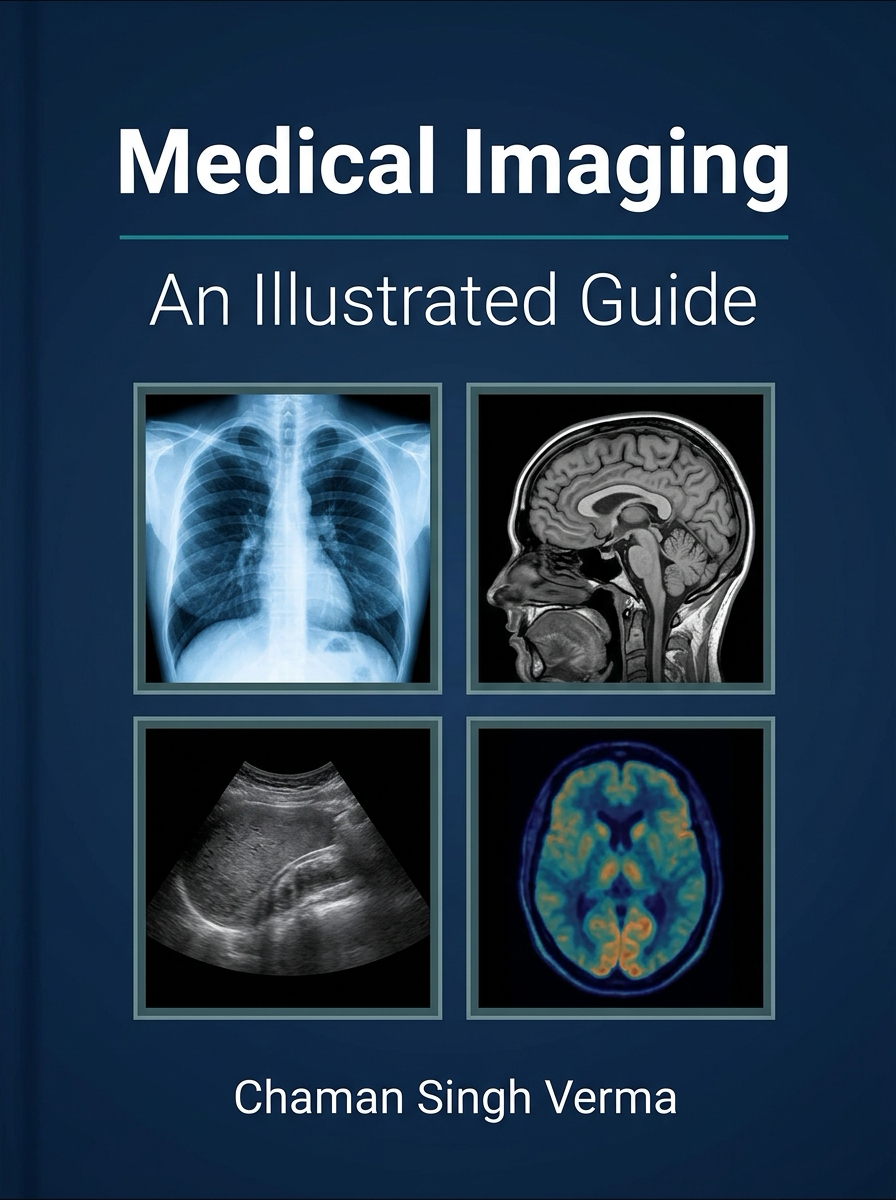
\includegraphics[width=\paperwidth,height=\paperheight]{cover.png}}
\null\clearpage
\maketitle
\thispagestyle{empty}
\vspace*{\fill}

\noindent\textbf{Medical Imaging: An Illustrated Guide}\\
Copyright \textcopyright\ 2026 Chaman Singh Verma.

\vspace{0.8em}
\noindent\textbf{License (MIT License)}\\
Permission is hereby granted, free of charge, to any person obtaining a copy of this work and associated documentation files, to deal in the work without restriction, including without limitation the rights to use, copy, modify, merge, publish, distribute, sublicense, and/or sell copies of the work, and to permit persons to whom the work is furnished to do so, subject to the following conditions: the above copyright notice and this permission notice shall be included in all copies or substantial portions of the work. The work is provided ``as is'', without warranty of any kind, express or implied.

\vspace{1.2em}
\noindent\textbf{Medical Disclaimer}\\
This book is intended strictly for educational and informational purposes. It is designed to help patients, families, students, and general readers understand how medical imaging technologies work, why clinicians order specific exams, and what to expect during a visit.

Nothing in this book constitutes medical advice, diagnosis, or treatment, nor should it be used to choose, delay, or decline any medical test or procedure. Imaging recommendations depend on an individual's full medical history, physical examination, laboratory results, pregnancy status, implanted devices, kidney function, and clinical urgency. Always consult a qualified physician, radiologist, or licensed healthcare professional regarding any symptoms, test results, or medical decisions.

Every effort has been made to align technical descriptions, radiation dose estimates, and safety guidelines with current recommendations from major radiology and health organizations (including the American College of Radiology, National Institutes of Health, Mayo Clinic, Cleveland Clinic, and leading academic medical centers). However, clinical guidelines, contrast protocols, and regulatory approvals evolve continuously. Research-stage and investigational modalities covered in this book are clearly identified as such and are not substitutes for established clinical imaging.

\vspace{1.2em}
\noindent Typeset in \LaTeX\ using Latin Modern typography.
\clearpage

\chapter*{Preface}
\addcontentsline{toc}{chapter}{Preface}

Modern medicine relies on an extraordinary range of imaging tools---from split-second X-rays and bedside ultrasound to high-field MRI, molecular PET/CT, and microscopic optical eye scans. Yet for most patients and students, the alphabet soup of acronyms (CT, CTA, CTP, DWI, DTI, MRA, MRCP, SPECT, OCTA) can feel overwhelming, especially when a scan has just been ordered for you or a loved one.

This illustrated guide was written to bridge the gap between technical radiology textbooks and everyday patient understanding. Each chapter pairs a visual overview with clear, plain-English explanations of how the technology works, what symptoms or clinical questions prompt a doctor to order it, how to prepare, what the exam feels like, and how specialists interpret normal and abnormal patterns.

\section*{How to Use This Book}
\begin{itemize}
  \item \textbf{Organized by Physical Energy (Parts I--VII):} After an introductory classification chapter, the book groups modalities into seven parts: X-Ray, Magnetic Field, Ultrasound, Nuclear Medicine, Optical, Photoacoustic and Electromagnetic, and Hybrid Imaging.
  \item \textbf{Start With Your Symptoms or Body Area:} If you are unsure which chapter applies to your situation, turn to \textbf{Appendix~\ref{app:quick-finder}} (\textit{Quick-Finder Guide}) at the back of the book to jump directly from common symptoms to the relevant chapters.
  \item \textbf{Compare Radiation and Safety:} Turn to \textbf{Appendix~\ref{app:radiation-chart}} (\textit{Radiation Dose and Safety Comparison Chart}) for a side-by-side comparison of zero-radiation modalities and typical ionizing-radiation doses expressed in everyday natural-background equivalents.
  \item \textbf{Clinical vs.\ Research-Stage Modalities:} Everyday hospital staples (such as X-ray, CT, MRI, ultrasound, PET/CT, and OCT) include full patient-visit sections covering preparation, what happens during the scan, and follow-up. Family overview chapters and strictly investigational research technologies (such as magnetic particle imaging, terahertz imaging, microwave imaging, and Raman spectroscopic imaging) are clearly distinguished so readers always know which tools are proven clinical standards and which remain in laboratory or prototype testing.
  \item \textbf{References and Further Reading:} Every chapter separates peer-reviewed clinical guidelines and institutional medical references (\textit{Key References}) from accessible general encyclopedic overviews (\textit{Further Reading}).
\end{itemize}

{\setlength{\parskip}{0pt}\tableofcontents}
\mainmatter
% --- Medical Imaging Classification ---
\infographicchapter{Medical Imaging Classification}{med_imaging_cls.png}
\label{ch:infographic-imaging-classification}

\section{Overview}

Medical imaging covers a wide range of tests that let doctors look inside the body without surgery. To make sense of all these tools, medicine organizes them into five main families based on the type of energy they use: X-ray imaging (standard X-rays, live fluoroscopy, mammograms, and CT scans), nuclear medicine (bone scans, SPECT, and PET), magnetic imaging (MRI, functional MRI, MEG, and research-stage MPI), sound-wave imaging (standard, blood-flow, and stiffness ultrasound), and light or electromagnetic-wave imaging (visible light, near-infrared, terahertz, microwave, and hybrid light-plus-sound photoacoustic systems).

Doctors also group scans by what kind of story they tell: \emph{anatomical} scans show body structure and shape, \emph{functional} scans show live movement or blood flow, and \emph{molecular} scans show cell metabolism or chemical targets. Most imaging tests are \emph{noninvasive}---meaning no surgical instrument enters the body---and span from simple \emph{visible-light} clinical photos (such as dermatology and wound checks) to flat \emph{projectional} 2D X-rays and \emph{tomographic} ``slice-by-slice'' 3D views like CT, MRI, PET, and SPECT. Scans also differ in whether they use ionizing radiation, how sharp their pictures are, how fast they run, how deeply they see into the body, and whether they can roll right up to a hospital bed. No single test is best at everything---CT is fast and sharp for emergencies but uses X-rays, PET spots tiny cellular changes across the whole body, and ultrasound works live at the bedside with zero radiation.

Understanding these groups helps doctors pick the safest, smartest test for your symptoms, avoid unnecessary radiation or costs, and combine complementary scans---such as PET/CT, SPECT/CT, or PET/MRI---when both structure and function are needed.

\section{Underlying Physical Principles}
\begin{itemize}
  \item \textbf{Passing X-Rays Through the Body (X-Ray and CT Family):} X-rays travel through you and get absorbed differently by each tissue. Dense bone absorbs lots of X-rays and looks bright white, air-filled lungs let X-rays pass right through and look dark, and soft organs sit in shades of gray.
  \item \textbf{Tracers Glowing From Inside (Nuclear Medicine Family):} A tiny dose of a radioactive tracer travels to specific organs or tumors and gives off gamma rays from inside the body. Outside cameras (SPECT or PET) detect those rays to map cell activity, blood flow, or tumor targets.
  \item \textbf{Magnets and Natural Brain Signals (Magnetic Family):} MRI uses strong magnets and harmless radio waves to gently nudge hydrogen atoms in body water and fat without any X-ray radiation. Passive MEG simply listens to the ultra-faint natural magnetic fields created by firing brain cells.
  \item \textbf{Bouncing Sound Waves (Ultrasound Family):} High-pitched sound waves (too high for human ears to hear) bounce off internal tissue edges to draw live pictures, track moving red blood cells (Doppler), and feel tissue stiffness (elastography).
  \item \textbf{Light and Gentle Radio-Range Waves (Optical and EM Family):} Visible light, near-infrared light, terahertz, and microwave tools measure how surface tissues absorb or scatter light, glow with safe dyes, create tiny heat-driven sound waves, or hold water---turning those clues into detailed surface maps.
\end{itemize}

\section{Imaging Mechanism}
\begin{enumerate}
  \item \textbf{Getting Positioned:} Across all five families, you are comfortably positioned with the right equipment---standing or lying by an X-ray plate or CT ring, lying inside a PET/SPECT or MRI scanner, sitting under a MEG helmet, resting with cool gel for an ultrasound probe, or sitting at an optical camera.
  \item \textbf{Sending or Listening for Signals:} Active machines send controlled X-rays, radio waves, sound pulses, or gentle light into the body (often timed to a breath-hold or heartbeat), while passive nuclear and MEG systems quietly record signals coming out from your body.
  \item \textbf{Capturing Digital Data:} Detectors, crystals, receiver coils, sound probes, or light sensors turn the returning energy into electrical signals and save them as digital files.
  \item \textbf{Building Clear Pictures:} Computers clean up background noise, correct for tissue shadows or motion, and assemble sharp 2D snapshots, live videos, or 3D cross-sectional volumes.
  \item \textbf{Reviewing and Blending:} Specialists adjust contrast, add color overlays, and blend hybrid scans together when needed. Hospitals store studies from every imaging family in a universal medical file format called \emph{DICOM} inside secure digital archives (\emph{PACS}), so any doctor on your care team can view them and compare them with future scans.
\end{enumerate}

\section{Key Technical Parameters}
\noindent
\begin{tabularx}{\textwidth}{@{}l X@{}}
\toprule
\textbf{Parameter} & \textbf{Typical Value / Description} \\
\midrule
Physical Principle & X-ray absorption (X-ray/CT), internal tracer rays (PET/SPECT), magnets and radio waves (MRI/MEG), sound echoes (ultrasound), and light or wave reflection (optical/EM) \\
Energy / Signal Source & X-ray tubes, radiotracers, magnets and radio coils, ultrasound probes, and medical lights or gentle wave emitters \\
Typical Frequency / Energy & 20--140 keV X-rays; 140--511 keV gamma rays; 1.5--3.0 Tesla MRI; 2--18 MHz sound waves; visible, near-infrared, THz, and microwave bands \\
Spatial Resolution & Ultra-fine under 1 mm (CT, mammograms, eye OCT) to 0.5--2 mm (MRI, ultrasound) and 3--10 mm (PET, SPECT, MEG) \\
Typical Scan Duration & Seconds (X-ray, CT) to 15--60 minutes (ultrasound, MRI, PET/SPECT) and 60--90 minutes (MEG) \\
Contrast Agent & Varies by scan: none, iodine or barium dye, gadolinium dye, radiotracers, tiny ultrasound microbubbles, or optical dyes \\
Ionizing Radiation & Yes for X-ray, CT, fluoroscopy, mammography, and nuclear medicine; zero for MRI, MEG, ultrasound, and optical/microwave/THz scans \\
\bottomrule
\end{tabularx}

\section{Clinical Usages}

\subsection{Primary Usages}
\begin{itemize}
  \item \textbf{Picking the Right First Test:} Grouping scans by how they work and what they show helps doctors follow trusted medical guidelines (such as the ACR Appropriateness Criteria) to choose the best test for your symptoms right away.
  \item \textbf{Diagnostic Screening vs. Image-Guided Treatment:} Clinical radiology spans \emph{diagnostic radiology}---screening for silent conditions (such as breast cancer, colon cancer, or heart disease), diagnosing symptoms, and tracking treatment response---and \emph{interventional radiology}, which uses live CT, ultrasound, MRI, or fluoroscopy to guide catheters, stents, biopsies, or tumor treatments through pinhole openings instead of open surgery, usually with only moderate sedation and rarely a hospital stay.
  \item \textbf{Protecting Patients From Unneeded Radiation:} Separating radiation-based scans (X-ray, CT, nuclear medicine) from radiation-free scans (ultrasound, MRI, optical) helps teams favor radiation-free options for children, pregnant patients, and people needing frequent checkups.
  \item \textbf{Combining Complementary Scans:} Seeing where each family shines---such as speed, fine detail, or cellular sensitivity---guides when to use hybrid scanners (PET/CT, SPECT/CT, PET/MRI) or step-by-step multi-scan workups in cancer, heart, and brain care.
  \item \textbf{Teaching and Clear Teamwork:} A shared map of imaging families helps doctors, technologists, physicists, and patients talk clearly about why a specific scan was chosen and what trade-offs it involves.
\end{itemize}

\subsection{Secondary Usages}
\begin{itemize}
  \item \textbf{Planning Hospital Equipment:} Health systems use these categories to balance bedside portable units, rapid emergency CT rooms, and specialized MRI or nuclear medicine suites.
  \item \textbf{Separating Proven Care From Research:} Clearly distinguishing everyday hospital scans from emerging research tools (like microwave, terahertz, or photoacoustic imaging) helps patients and regulators know which tests are proven standards.
  \item \textbf{Standardizing Clinical Research:} Clear categories help multicenter clinical trials keep scan settings and measurements consistent across different hospitals.
\end{itemize}

\section{Advantages}
\begin{itemize}
  \item \textbf{Smarter Test Selection:} Helps doctors match the exact right scan to each medical question instead of ordering unnecessary or low-value tests.
  \item \textbf{Clear Radiation Awareness:} Makes it easy to spot radiation-free choices for children, pregnant patients, and long-term monitoring.
  \item \textbf{Better Multi-Scan Strategy:} Shows how combining two families (like PET/CT or ultrasound plus MRI) fills in each test's blind spots.
  \item \textbf{Common Language Across Care Teams:} Gives radiologists, referring doctors, engineers, and patients a simple, organized way to compare imaging options.
\end{itemize}

\section{Disadvantages}
\begin{itemize}
  \item \textbf{Hybrid Tools Cross Boundaries:} Modern combined scanners---such as photoacoustic imaging, PET/MRI, and spectral CT---blend two physical families and do not fit neatly into just one box.
  \item \textbf{Mixing Everyday and Experimental Tools:} Listing proven hospital staples alongside early research tools in the same family can make experimental scans sound more widely available than they really are.
  \item \textbf{Does Not Reflect Local Access or Cost:} A physics-based chart cannot show which machines your local hospital has, how much a scan costs, or your personal medical limits (like claustrophobia or implants).
  \item \textbf{Technology Moves Fast:} Rapid advances in artificial intelligence, wearable brain sensors, and next-generation CT detectors keep blurring traditional lines between structure and function.
\end{itemize}

\section{Patient Safety Guidelines}
\begin{itemize}
  \item \textbf{Choosing Only Necessary Scans:} Doctors follow evidence-based guidelines to pick the safest scan that truly answers your medical question, avoiding duplicate or unnecessary tests.
  \item \textbf{Favoring Radiation-Free Options When Equal:} Whenever ultrasound or MRI can answer the question just as well as CT or X-ray, teams choose the radiation-free option---especially for children, pregnant patients, and repeat checkups.
  \item \textbf{Tailored Safety Checklists:} Each family has its own safety checklist: metal and kidney checks for MRI, pregnancy and dose checks for X-ray/CT/nuclear scans, safe heat limits for ultrasound, and eye-safe limits for medical light tools.
  \item \textbf{Safe Handling of Dyes and Tracers:} Before giving any contrast dye or radiotracer, staff check allergies, kidney health, pregnancy, and breastfeeding status, with emergency care ready just in case.
  \item \textbf{Clear Line Between Proven Care and Research:} Hospitals clearly separate FDA-cleared clinical scans from experimental platforms (such as microwave, terahertz, or MPI), which require ethics-board oversight and must never delay standard care.
\end{itemize}

\section{Augmenting Methods}
\begin{itemize}
  \item \textbf{Hybrid Scanners (PET/CT, SPECT/CT, PET/MRI):} Combine sharp anatomy with sensitive cellular activity in one visit, overcoming the limits of standalone scans.
  \item \textbf{Step-by-Step Multi-Scan Workups:} Pairing tests in sequence---like a mammogram or ultrasound followed by MRI, or an emergency CT followed by diffusion MRI---delivers the highest accuracy.
  \item \textbf{Blood and Lab Markers:} Lab tests like PSA, heart troponins, D-dimer, hormone panels, or DNA blood tests provide vital clues that narrow down what an imaging spot means.
  \item \textbf{Tissue Biopsy and Genetic Testing:} Image-guided needle biopsies and lab pathology remain the final gold standard for confirming uncertain lumps across all scan families.
  \item \textbf{Computer Fusion and Smart AI Tools:} Software that lines up past and present scans, uses structured report templates, and flags urgent findings helps teams work faster and more accurately.
\end{itemize}

\section{Comparison with Alternative Modalities}
\begin{itemize}
  \item \textbf{Structure vs. Function:} X-ray, CT, and standard MRI excel at showing shape and anatomy, while PET, SPECT, fMRI, and MEG catch early chemical, metabolic, or electrical changes before structural damage appears.
  \item \textbf{Radiation vs. Radiation-Free:} CT and nuclear medicine provide rapid emergency answers or whole-body cellular reach with controlled radiation, while ultrasound, MRI, and optical scans allow safe repeated checks for children and pregnant patients.
  \item \textbf{Deep Whole-Body vs. Portable Surface Scans:} CT, MRI, and PET/CT inspect deep organs throughout the body, whereas ultrasound and optical tools trade depth for bedside portability, live guidance, and microscopic surface clarity.
  \item \textbf{Single Scan vs. Hybrid Scan:} A single focused scan is faster and less expensive for straightforward questions, while hybrid scanners shine for complex cancer staging, heart viability, and brain care.
\end{itemize}

\section{Key References}
\begin{itemize}
  \item American College of Radiology (ACR). \textit{ACR Appropriateness Criteria}. Reston, VA: American College of Radiology, 2024.
  \item Bushberg JT, Seibert JA, Leidholdt EM, Boone JM. \textit{The Essential Physics of Medical Imaging}. 4th ed. Philadelphia, PA: Wolters Kluwer, 2020.
  \item National Institute of Biomedical Imaging and Bioengineering (NIBIB). \textit{Science Topics: Medical Imaging Modalities Overview}. Bethesda, MD: National Institutes of Health, 2024.
  \item International Commission on Radiological Protection (ICRP). \textit{The 2007 Recommendations of the International Commission on Radiological Protection (ICRP Publication 103)}. Oxford: Elsevier, 2007.
  \item MedlinePlus Medical Encyclopedia. \textit{Imaging and radiology}. U.S. National Library of Medicine, National Institutes of Health. Available at: \url{https://medlineplus.gov/ency/article/007451.htm}.
\end{itemize}

\section{Further Reading}
\begin{itemize}
  \item Wikipedia contributors. \textit{Medical imaging}. Wikipedia, The Free Encyclopedia. Available at: \url{https://en.wikipedia.org/wiki/Medical_imaging}.
\end{itemize}


% --- Part I: X-Ray Imaging Modalities ---
\part{X-Ray Imaging Modalities}
\infographicchapter{X-ray Imaging Modalities}{xray_cls.png}
\label{ch:infographic-xray-imaging-overview}

\section{Overview}

First discovered by physicist Wilhelm Conrad R\"ontgen in 1895, X-ray imaging is the foundational family of medical scans that uses carefully controlled beams of X-ray energy to look inside the body. As the beam passes through you toward a digital sensor, different tissues block different amounts of X-rays depending on how dense and thick they are. Hard, dense structures like bones and metal implants block most X-rays and show up bright white. Air-filled lungs let almost all X-rays pass right through and look dark black, while muscles, organs, and fat appear in shades of gray.

The X-ray family includes both quick 2D snapshots and detailed 3D cross-sectional scans. Standard plain X-rays are the fast first choice for broken bones, chest infections, and checking medical tubes. Mammograms and 3D breast tomosynthesis use gentle, low-energy X-rays tailored to spot early breast lumps and tiny calcium specks. Fluoroscopy and angiography act like live X-ray movies to guide blood-vessel procedures, swallowing studies, and bone repairs, often using contrast dye to make vessels or digestive organs stand out. Computed tomography (CT) spins an X-ray beam around your body to build sharp 3D slices for trauma, strokes, cancer, and heart care, DEXA scans use an ultra-low dose to measure bone strength for osteoporosis, and specialized slot-scanning X-ray systems capture full-length standing views of the spine and legs at very low dose.

Doctors rely on X-ray scans every day because they are fast, widely available, and show crisp anatomical detail. Because X-rays use ionizing radiation, medical teams follow strict ALARA (``as low as reasonably achievable'') rules to keep doses as small as possible, with special care for children and pregnant patients.

\section{Underlying Physical Principles}
\begin{itemize}
  \item \textbf{Creating a Controlled X-Ray Beam:} Inside a shielded X-ray tube, fast-moving electrons strike a spinning metal target (usually tungsten, or molybdenum/rhodium for mammograms), producing a focused beam of X-rays shaped tightly to the body part being checked.
  \item \textbf{How Tissues Create the Picture:} As X-rays pass through the body, tissues reduce (attenuate) the beam based on their thickness, physical density, and atomic number. Radiologists describe structures that block most rays and look bright white---such as bone, metal, or contrast dye---as \emph{radiopaque}, while structures that let most rays pass through and look dark---such as air-filled lungs or fat---are called \emph{radiolucent}, creating five classic shades from black air to dark-gray fat, gray soft tissue and fluid, white bone, and brilliant white metal. Some rays scatter slightly, which anti-scatter grids and digital software filter out.
  \item \textbf{Flat 2D Pictures vs. 3D CT Slices:} Plain X-rays, mammograms, and fluoroscopy capture flat 2D shadow pictures on digital panels. CT scanners spin the X-ray tube and detectors all the way around your body to gather views from every angle and build 3D slices.
  \item \textbf{Dual-Energy and Photon-Counting Detail:} Advanced DEXA, dual-energy CT, and newer photon-counting CT measure X-rays at different energy levels to tell materials apart---such as separating bone mineral, kidney-stone types, gout crystals, and contrast dye.
  \item \textbf{Standard Density Scale (Hounsfield Units):} CT software turns raw scan data into sharp 3D volumes using a standard brightness scale (Hounsfield units), where air is very negative, water is zero, and dense bone is high positive.
\end{itemize}

\section{Imaging Mechanism}
\begin{enumerate}
  \item \textbf{Positioning and Focusing the Beam:} You stand against a digital plate (for chest or limb X-rays and mammograms), lie on a motorized table gliding through a wide CT ring, or lie beneath a fluoroscopy arm. Built-in shutters narrow the beam strictly to the area being examined.
  \item \textbf{Brief, Controlled Exposure:} Automatic exposure controls deliver just enough X-ray energy for your body size---capturing a split-second snapshot (plain X-ray or DEXA), a short angled sweep (3D mammogram), pulsed live video (fluoroscopy), or a fast 360-degree spin (CT).
  \item \textbf{Digital Detection:} Digital flat panels or CT detector rings catch the X-rays that pass through your body and convert them immediately into digital signals.
  \item \textbf{Cleaning Up and Building the Image:} Computers correct for scatter and metal glare, subtract background structures (in blood-vessel angiography), or reconstruct crisp 3D CT slices using modern low-dose and AI software.
  \item \textbf{Viewing and Saving:} Radiologists view the images using tailored contrast settings (such as bone, lung, soft-tissue, or 3D blood-vessel views) on high-definition monitors and save them to your medical record.
\end{enumerate}

\section{Key Technical Parameters}
\noindent
\begin{tabularx}{\textwidth}{@{}l X@{}}
\toprule
\textbf{Parameter} & \textbf{Typical Value / Description} \\
\midrule
Physical Principle & Controlled X-ray beams pass through the body and are blocked differently by bone, soft tissue, fat, air, or contrast dye \\
Energy / Signal Source & X-ray tubes paired with digital flat panels, CT detector rings, or fluoroscopy screens \\
Typical Frequency / Energy & 25--35~kVp (mammography), 60--120~kVp (plain X-ray/fluoroscopy), 80--140~kVp (CT); typical dose ranges from 0.001--0.1~mSv (DEXA/chest X-ray) to 2--15~mSv (CT) \\
Spatial Resolution & About 0.05--0.2~mm (mammography and plain X-ray); 0.25--0.6~mm in 3D (modern CT) \\
Typical Scan Duration & Seconds of actual X-ray exposure (5--20~minutes total visit for X-ray, mammogram, DEXA, or CT); 30--90~minutes for interventional angiography \\
Contrast Agent & None for routine X-rays, mammograms, DEXA, or non-contrast CT; optional IV or oral iodine dye or oral barium for CT and fluoroscopy \\
Ionizing Radiation & Yes (external X-ray beam managed strictly under ALARA safety rules) \\
\bottomrule
\end{tabularx}

\section{Clinical Usages}

\subsection{Primary Usages}
\begin{itemize}
  \item \textbf{Broken Bones, Injuries, and Chest Checks:} Plain X-rays and CT scans are the fast first-line tools for fractures, dislocated joints, osteoarthritis, spine curvature (such as scoliosis), pneumonia, collapsed lungs, swallowed or lodged foreign objects, medical line checks, and major trauma.
  \item \textbf{Stroke and Blood-Vessel Emergencies:} A quick non-contrast head CT immediately checks for brain bleeding in stroke or head injury, while CT angiography (CTA) and catheter angiography (DSA) spot blocked brain arteries, aneurysms, lung clots, and aortic tears.
  \item \textbf{Breast Cancer Screening and Diagnosis:} Digital mammography and 3D breast tomosynthesis are the primary proven screening tests to spot early breast lumps and tiny calcium specks (microcalcifications).
  \item \textbf{Cancer Staging and Belly Emergencies:} Contrast CT of the chest, abdomen, and pelvis stages cancers, tracks treatment, and quickly diagnoses appendicitis, bowel blockages, and kidney stones.
  \item \textbf{Live Procedure Guidance:} Fluoroscopy and angiography guide heart stents, stroke clot removal, valve replacements, fracture repairs, and swallowing studies in real time.
\end{itemize}

\subsection{Secondary Usages}
\begin{itemize}
  \item \textbf{Bone Density Screening (DEXA):} Dual-energy X-ray absorptiometry (DEXA) is the clinical standard for checking osteoporosis, estimating fracture risk, and tracking bone-strengthening treatments.
  \item \textbf{Material-Specific Spectral CT:} Dual-energy and photon-counting CT help identify kidney-stone makeup, spot gout crystals in joints, and map blood flow in the lungs or heart.
  \item \textbf{CT-Guided Biopsies and Treatments:} Live CT slices guide precise needle biopsies, abscess drainages, tumor heat treatments, and targeted spine pain injections.
  \item \textbf{Radiation Therapy Planning and Dental Scans:} Specialized CT scanners map exact body geometry for cancer radiation therapy, while dental X-rays and cone-beam CT guide fillings, root canals, and dental implants.
\end{itemize}

\section{Advantages}
\begin{itemize}
  \item \textbf{Fast and Ready for Emergencies:} Plain X-rays and CT scans capture life-saving images in seconds, making them indispensable for severe trauma, stroke, and unstable patients.
  \item \textbf{Sharp Detail for Bone, Lungs, and Calcium:} X-rays clearly show hairline fractures, lung tissue, contrast-filled blood vessels, and tiny breast calcifications.
  \item \textbf{Available Almost Everywhere:} X-ray and CT machines are standard across hospitals and clinics worldwide, with plain X-rays being especially quick and affordable.
  \item \textbf{Live Guidance for Minimally Invasive Procedures:} Fluoroscopy and angiography let specialists guide catheters, stents, and surgical screws safely without large open incisions.
  \item \textbf{Full 3D and Quantitative Views:} Modern CT creates crisp 3D views from any angle, while DEXA provides standardized bone-strength scores.
\end{itemize}

\section{Disadvantages}
\begin{itemize}
  \item \textbf{Ionizing Radiation Exposure:} X-rays carry a small long-term radiation risk---and very long fluoroscopy procedures can occasionally cause skin redness---so every scan must be justified under ALARA rules, especially in children and pregnancy.
  \item \textbf{Less Soft-Tissue Detail Than MRI:} Without contrast dye, X-rays and CT show less fine soft-tissue detail than MRI for the brain, spinal cord, ligaments, cartilage, and pelvic organs.
  \item \textbf{Contrast Dye Side Effects:} IV iodine contrast used in CT and angiography carries small risks of allergic-like reactions, temporary kidney strain in severe kidney disease, or rare thyroid flares.
  \item \textbf{Overlapping Shadows and Metal Glare:} Flat 2D X-rays stack structures on top of each other, while CT can show streaks from metal implants, dental fillings, or patient movement.
  \item \textbf{Shows Structure Rather Than Cell Activity:} Standard X-rays show body shape and density rather than direct cell metabolism or chemical activity.
\end{itemize}

\section{Patient Safety Guidelines}
\begin{itemize}
  \item \textbf{Keeping Radiation Low (ALARA):} Teams confirm every scan is needed, tailor doses to body size (using child-sized Image Gently and adult Image Wisely protocols), narrow the beam tightly, and audit doses regularly. Because children are more sensitive to radiation and have more years of life ahead, parents are encouraged to ask whether machine settings have been adjusted for a child's size.
  \item \textbf{Careful Fluoroscopy Monitoring:} During live X-ray procedures, doctors use brief pulsed beams, freeze-frame holds, and dose tracking, arranging a quick skin check 2 to 4~weeks later if a long complex procedure ever reaches high skin-dose thresholds.
  \item \textbf{Pregnancy Checks and Updated Shielding Rules:} Staff check for possible pregnancy before belly, pelvic, or higher-dose exams; when imaging areas away from the abdomen or pelvis (such as a limb or tooth), diagnostic X-rays pose no known risk to a developing baby. Following updated ACR and AAPM safety guidance, routine lead aprons over the belly or pelvis are no longer recommended because they can interfere with modern automatic dose controls.
  \item \textbf{Contrast Dye Safety:} Staff screen for prior dye reactions, check kidney function (eGFR) in at-risk patients, give clear instructions about metformin diabetes pills if needed, keep allergy treatments ready, and avoid barium if a bowel tear is suspected.
  \item \textbf{Equipment Checks and Staff Protection:} Medical physicists test X-ray and CT machines regularly to ensure accurate dosing, and staff wear lead aprons and radiation badges during fluoroscopy or bedside exams.
\end{itemize}

\section{Augmenting Methods}
\begin{itemize}
  \item \textbf{MRI:} Radiation-free MRI pairs with X-ray and CT to give unmatched soft-tissue detail for the brain, spine, bone marrow, ligaments, cartilage, and pelvis.
  \item \textbf{Targeted Ultrasound:} Bedside ultrasound helps evaluate dense breasts after mammography, checks gallbladders and kidneys without radiation, and guides fluid drainages.
  \item \textbf{Nuclear Medicine (PET/CT and Bone Scans):} PET/CT and SPECT/CT add cell-activity and cancer-metabolism insight to sharp CT anatomy.
  \item \textbf{Blood Tests and Guided Biopsies:} Labs like D-dimer, troponin, and blood counts guide CT decisions, while mammogram- or CT-guided core biopsies provide definitive lab answers.
  \item \textbf{Spectral CT and AI Triage:} Dual-energy and photon-counting CT, low-dose AI reconstruction, and FDA-cleared AI alert tools help radiologists spot brain bleeds, lung clots, collapsed lungs, and breast changes faster and more accurately.
\end{itemize}

\section{Comparison with Alternative Modalities}
\begin{itemize}
  \item \textbf{Versus MRI:} X-ray and CT are much faster, cost less, excel in emergencies, and show bone, lungs, fresh bleeding, and calcium better, while MRI gives unmatched soft-tissue detail with zero ionizing radiation.
  \item \textbf{Versus Ultrasound:} X-ray and CT give broad views unaffected by bone or bowel gas and do not depend on operator skill, while ultrasound uses no radiation and is the top first choice for pregnancy, children, gallbladders, and bedside checks.
  \item \textbf{Versus Nuclear Medicine:} CT shows crisp sub-millimeter anatomy in seconds, while nuclear medicine reveals early cellular activity (making combined PET/CT especially powerful).
  \item \textbf{Plain X-Ray Versus CT:} Plain X-rays use an ultra-low dose at minimal cost for initial bone or chest checks, while CT removes overlapping shadows to give full 3D clarity for trauma, blood vessels, and cancer care.
\end{itemize}

\section{Key References}
\begin{itemize}
  \item American College of Radiology (ACR) Committee on Drugs and Contrast Media. \textit{ACR Manual on Contrast Media}. Reston, VA: American College of Radiology, 2024.
  \item International Commission on Radiological Protection (ICRP). \textit{Managing Patient Dose in Multi-Detector Computed Tomography (MDCT) (ICRP Publication 102)}. Oxford: Elsevier, 2007.
  \item American Association of Physicists in Medicine (AAPM). \textit{AAPM Position Statement on the Use of Patient Gonadal and Fetal Shielding}. Alexandria, VA: AAPM, 2019.
  \item Bushberg JT, Seibert JA, Leidholdt EM, Boone JM. \textit{The Essential Physics of Medical Imaging}. 4th ed. Philadelphia, PA: Wolters Kluwer, 2020.
  \item National Institute of Biomedical Imaging and Bioengineering (NIBIB). \textit{Medical X-rays}. National Institutes of Health (NIH). Available at: \url{https://www.nibib.nih.gov/science-education/science-topics/medical-x-rays}.
  \item Radiopaedia.org. \textit{General radiography}. Radiopaedia. Available at: \url{https://radiopaedia.org/articles/general-radiography}.
\end{itemize}

\section{Further Reading}
\begin{itemize}
  \item Wikipedia contributors. \textit{Radiography}. Wikipedia, The Free Encyclopedia. Available at: \url{https://en.wikipedia.org/wiki/Radiography}.
\end{itemize}

\infographicchapter{X-Ray Imaging}{xray.png}
\label{ch:infographic-xray}

\section{Overview}

X-ray imaging---also called radiography---is the oldest, fastest, and most widely used medical imaging test in the world. It creates clear, two-dimensional shadow pictures of the inside of your body in a fraction of a second using a tiny, controlled burst of high-energy light called X-rays. As the X-ray beam passes through your body to a digital sensor plate, dense materials like bone and metal block more of the beam and show up bright white; air-filled spaces like your lungs let most of the beam pass through and appear dark black; and soft tissues like muscle, fat, and organs show up in shades of gray.

Doctors rely on X-rays every day to check bones and joints for fractures, dislocations, arthritis, and surgical hardware; to inspect the chest for pneumonia, collapsed lungs, fluid buildup, or heart enlargement; to check the abdomen for bowel blockages or swallowed objects; to examine teeth in dental care; and to verify that hospital breathing tubes, IV lines, or pacemakers sit in the exact right place.

X-rays are fast, painless, inexpensive, available almost everywhere, and even portable enough to roll right to a hospital bedside. Their main limits are that they flatten 3D anatomy into a 2D picture---so overlapping ribs or bones can hide subtle problems, often requiring two or three views from different angles---and they do not show soft tissues like ligaments or organs as clearly as CT or MRI. Because X-rays use a small amount of ionizing radiation---a single chest X-ray delivers roughly the same dose as about 10 days of natural background radiation from the environment---clinics always make sure every scan is truly needed and keep the dose as low as reasonably achievable (ALARA), taking extra care for children and pregnant patients.

\section{Underlying Physical Principles}

\begin{itemize}
    \item \textbf{Creating the X-Ray Beam:} Inside the X-ray tube, a tiny heated wire releases electrons that speed across a high-voltage gap and strike a metal tungsten target. That sudden impact releases a controlled burst of invisible, high-energy X-ray light.
    \item \textbf{How Body Tissues Create Light and Dark Shades:} As X-rays pass through your body, tissues absorb them based on their thickness, density, and atomic makeup, creating five classic shades from black to bright white: air in the lungs or bowel lets almost all X-rays pass through (called \textit{radiolucent}) and looks black; fat looks dark gray; muscle, organs, and fluid look medium gray; calcium-rich bone looks white; and metal hardware blocks nearly the entire beam (called \textit{radiopaque}) and looks brightest white.
    \item \textbf{Sharpening the Picture and Digital Capture:} Adjustable metal shutters narrow the beam strictly to the body part being checked, and a thin grid filters out stray scattered rays. The clean beam then strikes a modern digital flat-panel detector that turns the X-ray pattern directly into electrical signals.
    \item \textbf{Turning Signals Into a Clear Image:} Built-in electronics read every pixel on the detector and computer software balances brightness and sharpens edges, displaying a crisp black-and-white radiograph within seconds.
\end{itemize}

\section{Imaging Mechanism}

\begin{enumerate}
    \item \textbf{Positioning and Narrowing the Beam:} You stand, sit, or lie against a flat digital detector plate while the technologist lines up the X-ray tube at a set distance and narrows the light-guided beam tightly to the exact area being examined.
    \item \textbf{Quick Controlled Exposure:} The technologist sets the tailored power for your body part (often using automatic sensors that shut off the beam the instant the picture is bright enough) and triggers a fraction-of-a-second X-ray burst while you hold still or pause your breath.
    \item \textbf{Digital Capture:} X-rays passing through your body hit the digital flat-panel sensor, creating electrical charges at millions of tiny pixels that are converted into digital numbers.
    \item \textbf{Automatic Image Polish:} The workstation automatically calibrates the detector, balances contrast across thick and thin areas, and sharpens fine bone and lung edges.
    \item \textbf{Instant Check and Review:} Within seconds, the crisp 2D image appears on the technologist's screen to check positioning and clarity before being sent to the radiologist for formal interpretation.
\end{enumerate}

\section{Key Technical Parameters}

\noindent
\begin{tabularx}{\textwidth}{@{}l X@{}}
\toprule
\textbf{Parameter} & \textbf{Typical Value / Description} \\
\midrule
Physical Principle & Different body tissues absorb X-rays at different rates to cast a sharp 2D shadow picture on a digital plate \\
Energy / Signal Source & High-voltage X-ray tube \\
Typical Frequency / Energy & 50--70 kVp (hands, feet, limbs); 70--90 kVp (abdomen and spine); 100--125 kVp (chest) \\
Spatial Resolution & Very sharp (about 0.1--0.2 mm pixel detail on modern digital flat panels) \\
Typical Scan Duration & Fractions of a second per picture; 5--15 minutes total for a multi-angle set \\
Contrast Agent & None for standard X-rays (barium or iodine dyes are used only in specialized fluoroscopy exams) \\
Ionizing Radiation & Yes, very low dose (about 0.001 mSv for a limb, 0.02--0.1 mSv for a chest, and 0.7--1.5 mSv for abdomen or lower spine) \\
\bottomrule
\end{tabularx}

\section{Common Symptoms That Prompt This Scan}
\begin{itemize}
    \item \textbf{Bone or Joint Pain After an Injury:} Localized swelling, bruising, tenderness, deformity, or inability to bear weight on a limb after a fall, twist, or impact.
    \item \textbf{Persistent Cough or Breathing Trouble:} Fever with a productive cough, shortness of breath, sharp chest pain when inhaling, or unexplained wheezing.
    \item \textbf{Ongoing Joint Stiffness or Swelling:} Chronic knee, hip, hand, or back pain and stiffness that worsen with standing or daily movement.
    \item \textbf{Sudden Severe Belly Pain or Vomiting:} Abdominal bloating, inability to pass gas, repeated vomiting, or suspected swallowed foreign objects.
    \item \textbf{Toothache or Facial Injury:} Localized tooth pain, gum swelling, or jaw tenderness after a bump or fall.
\end{itemize}

\section{Clinical Usages}

\subsection{Primary Usages}

\begin{itemize}
    \item \textbf{Broken Bones and Joints:} The first-choice exam for fractures, dislocations, osteoarthritis, joint inflammation, bone growths, and checking metal plates, screws, or joint replacements after orthopedic surgery.
    \item \textbf{Chest and Lung Checks:} Quick first look for pneumonia, a collapsed lung (pneumothorax), fluid around the lungs (pleural effusion), lung congestion from heart failure, enlarged heart, or larger chest masses.
    \item \textbf{Checking Medical Tubes and Devices:} Confirming safe placement of breathing tubes, central IV lines, feeding tubes, chest drains, and pacemakers.
    \item \textbf{Sudden Belly Pain Screening:} Fast check for bowel blockages, free air from a perforated bowel, or swallowed metal objects and certain stones.
    \item \textbf{Dental Care:} Everyday checks for cavities, tooth root infections, gum bone loss, impacted wisdom teeth, and jaw injuries.
\end{itemize}

\subsection{Secondary Usages}

\begin{itemize}
    \item \textbf{Tracking Healing Over Time:} Checking how well a broken bone is knitting together, confirming pneumonia or a collapsed lung has cleared, and checking artificial joints over the years for loosening.
    \item \textbf{Bone Surveys and Childhood Growth:} Evaluating suspected bone conditions, multiple myeloma, or checking a child's bone age and growth plates.
    \item \textbf{Workplace and Public Health Screening:} Screening for dust-related lung conditions (like silicosis or asbestosis) or active tuberculosis in higher-risk groups.
    \item \textbf{Standing and Bending Views:} Taking X-rays while standing on your feet or gently bending your neck or back to spot joint-space narrowing or spine movement issues that only show up under normal body weight.
\end{itemize}

\section{Advantages}

\begin{itemize}
    \item \textbf{Fast and Everywhere:} Produces clear pictures in seconds on equipment found in clinics, urgent cares, dental offices, and hospitals worldwide.
    \item \textbf{Low Cost and High Efficiency:} The most affordable medical imaging test, making it ideal for first-step evaluation and routine healing checks.
    \item \textbf{Bedside Portability:} Mobile X-ray machines roll directly into hospital rooms, ICUs, or operating rooms so very sick or injured patients do not have to be moved.
    \item \textbf{Razor-Sharp Bone and Hardware Detail:} Clearly shows fine bone cracks, joint alignment, swallowed metal, and medical tubes at a very low radiation dose per picture.
    \item \textbf{Shows Real-World Weight-Bearing:} Easily captures standing knees, feet, or bending spine views to reveal how joints behave under everyday weight.
\end{itemize}

\section{Disadvantages}

\begin{itemize}
    \item \textbf{Flattens 3D Into 2D:} Overlapping ribs, collarbones, or neighboring bones can hide tiny fractures or small lung spots, which is why technologists usually take two or three views from different angles.
    \item \textbf{Limited Soft-Tissue Detail:} Soft tissues like muscles, ligaments, cartilage, and solid organs look very similar in gray tones, so CT, MRI, or ultrasound is needed for deeper soft-tissue questions.
    \item \textbf{Small Ionizing Radiation Dose:} Although very low per picture, X-rays use ionizing radiation, so clinics follow ALARA safety rules and take special care with children and pregnant patients.
    \item \textbf{Positioning Can Distort Size:} Like a flashlight casting a larger shadow when your hand moves farther from the wall, structures farther from the detector plate appear slightly magnified. For routine chest X-rays, the beam enters from your back (a PA view) so your heart rests right against the plate for true-to-life sizing; portable bedside views enter from the front (an AP view), which---along with slight rotation or shallow breaths---can make a normal heart look artificially enlarged.
    \item \textbf{Still Snapshots Only:} Standard X-rays show static structure rather than live blood flow, heart pumping, or organ metabolism.
\end{itemize}

\section{Contraindications}

\subsection{Absolute}

\begin{itemize}
    \item \textbf{None When Medically Needed:} There are no strict absolute contraindications to an X-ray when a doctor determines it is clinically necessary, because the diagnostic benefit in injuries or chest emergencies far outweighs the tiny radiation dose.
\end{itemize}

\subsection{Relative}

\begin{itemize}
    \item \textbf{Pregnancy:} Non-urgent belly, pelvis, or lower-spine X-rays are usually postponed during pregnancy if radiation-free ultrasound or MRI can answer the question. When an X-ray is truly needed, tight beam narrowing and low-dose settings keep fetal exposure extremely small.
    \item \textbf{Avoiding Unneeded Repeats in Children:} Extra non-essential X-rays in children are avoided whenever ultrasound or clinical follow-up is equally effective.
\end{itemize}

\section{Patient Safety Guidelines}

\begin{itemize}
    \item \textbf{Right Test, Lowest Dose (ALARA):} Every X-ray is checked for clear medical need, and technologists use automatic exposure controls and child-sized weight-based settings to keep radiation as low as reasonably achievable.
    \item \textbf{Tight Beam Focus and Avoiding Repeats:} Metal shutters narrow the X-ray beam strictly to the area being checked, and clear positioning and breath-hold coaching help get a crisp picture on the very first try.
    \item \textbf{Pregnancy Screening:} Staff ask anyone who could be pregnant before taking belly, pelvis, or lower-back X-rays so radiation-free options can be considered or the beam can be carefully tailored.
    \item \textbf{Modern Shielding Guidance:} Leading radiology organizations (AAPM, NCRP, and ACR) no longer recommend routine lead aprons directly over the pelvis or belly during an X-ray, because misplaced shields can cover needed anatomy or trick automatic sensors into raising the radiation dose. Tight beam focusing is safer and more effective.
    \item \textbf{Protecting Staff and Helpers:} Technologists step behind protective barriers during the brief exposure, and any parent or caregiver helping steady a child wears a protective lead apron.
\end{itemize}

\section{Prerequisite Tests}

\begin{itemize}
    \item \textbf{No Blood Tests or Fasting Needed:} Standard X-rays are noninvasive and dye-free, so no blood work or fasting is required.
    \item \textbf{Pregnancy Check (When Relevant):} Before abdominal, pelvic, or lower-spine X-rays in patients who could be pregnant, staff confirm pregnancy status---using a quick urine or blood pregnancy test if there is any uncertainty.
    \item \textbf{History and Past X-Rays:} Knowing where you hurt, how an injury happened, and reviewing any prior X-rays helps the technologist choose the exact right angles and helps the radiologist spot new changes.
    \item \textbf{Quick Metal Check:} Checking the area to remove necklaces, watches, zippers, or snaps prevents distracting white shadows and repeat shots.
\end{itemize}

\section{Preparing for the Scan}

\begin{itemize}
    \item \textbf{Remove Metal Near the Scan Area:} Take off jewelry, watches, glasses, hairpins, removable dentures, underwire bras, and clothing with metal zippers, snaps, or buttons over the body part being X-rayed so they do not block the picture.
    \item \textbf{Comfortable Clothing or a Gown:} Wear loose, metal-free clothing or change into a soft hospital gown if asked, making it easy to position the area accurately.
    \item \textbf{Eat and Take Medicines Normally:} Standard X-rays require no fasting, special drinks, or medicine changes (only specialized contrast X-ray studies using barium or iodine require fasting or a contrast drink beforehand).
    \item \textbf{Ready to Hold Still Briefly:} Follow the technologist's cues for standing, sitting, or lying in position, and practice taking a deep breath and holding it for a couple of seconds if you are having a chest X-ray.
    \item \textbf{Share Pregnancy or Pain Limits:} Tell the technologist before stepping in if you might be pregnant, recently had surgery, or have pain or balance trouble so they can cushion and support you safely.
\end{itemize}

\section{During Scan}

\begin{itemize}
    \item \textbf{Getting Into Position:} Depending on the body part, you will stand against an upright plate, sit beside a table, or lie comfortably on the X-ray table while the technologist lines up the camera. Holding completely still keeps the picture razor sharp.
    \item \textbf{Simple Breath-Holds:} For chest and some belly X-rays, you will be asked to take a deep breath in and hold it for 2--3 seconds so your lungs expand fully. Arm, hand, leg, or foot X-rays usually just need you to hold the limb still.
    \item \textbf{What It Feels and Sounds Like:} You cannot feel X-rays at all---the test is completely painless. You will only notice the cool surface of the plate, soft positioning sponges, and a quick click or beep when the picture snaps.
    \item \textbf{Constant Visual and Voice Contact:} The technologist steps behind a clear window during the split-second exposure while watching and talking with you. Speak up immediately if pain, dizziness, or stiffness makes holding a pose hard.
    \item \textbf{Fast Visit:} Each picture takes less than a second, and a full set of two or three angles usually finishes in 5--15 minutes, with short pauses while the technologist checks that every shot is crisp.
\end{itemize}

\section{Normal Appearance}

\begin{itemize}
    \item \textbf{Healthy Chest X-Ray:} Both lungs look evenly dark and full of air with sharp bottom corners, a centered windpipe, a normal-sized heart shadow, and smooth outlines along the diaphragm and chest center.
    \item \textbf{Healthy Bone and Joint X-Ray:} Bones show smooth, unbroken bright white outer rims, even inner bone texture, neat open joint spaces, and smooth surrounding soft tissues with no swelling.
    \item \textbf{Healthy Belly X-Ray:} Modest, non-stretched pockets of normal gas in the stomach and colon, with no free air under the diaphragm and no unusual bright stones or blockages.
\end{itemize}

\section{Observing for Abnormal Patterns}

\begin{itemize}
    \item \textbf{Lung Infection and Fluid Buildup:} Cloudy white patches in the dark lungs point to pneumonia, bleeding, or fluid filling the air sacs. Spreading haziness from the center of the chest, fine horizontal lines, and blunted lower lung corners signal heart-related lung congestion or fluid around the lungs (pleural effusion).
    \item \textbf{Collapsed Lung and Free Belly Air:} A thin white lung edge pulled away from the ribcage with empty dark air outside it identifies a collapsed lung (pneumothorax)---and if the heart shifts away, it signals an urgent tension pneumothorax. A thin dark crescent of air under the diaphragm on an upright view signals a bowel perforation.
    \item \textbf{Broken Bones and Hidden Joint Clues:} Cracks, dark fracture lines, buckled bone edges (common in children), or shifted joints confirm fractures. Even when a tiny elbow fracture is hidden, a lifted dark fat-pad shadow (``sail sign'') alerts doctors to look closer.
    \item \textbf{Bowel Blockages:} Stretched, gas-filled loops of small or large bowel stacked with flat fluid levels on upright views point to a bowel blockage or twisted bowel (volvulus).
    \item \textbf{Positioning Look-Alikes:} Taking a chest X-ray lying down or without a full deep breath can make a normal heart look artificially large or crowd the lower lungs, and skin folds, shoulder blades, or hospital tubing can occasionally mimic a collapsed-lung line.
\end{itemize}

\section{Dealing with Uncertainties}

\begin{itemize}
    \item \textbf{Overlapping Bones and Angles:} Ribs, collarbones, or neighboring bones can hide tiny hairline cracks or small lung spots, and slight rotation or shallow breathing can skew heart size or lung clarity.
    \item \textbf{Movement and Clothing Shadows:} Moving during the shot, breathing too soon, or leaving behind a zipper, button, or necklace can blur bone edges or mimic a lung spot.
    \item \textbf{Soft-Tissue Limits:} Because soft tissues, fluid, and infection look very similar in shades of gray, a plain X-ray cannot always tell apart a harmless scar, mild pneumonia, or an early lung nodule, nor can it see sprained ligaments or hidden hairline wrist and hip cracks.
    \item \textbf{Extra Views Right Away:} If a picture is blurred or overlapping bones hide an area, the technologist can quickly retake the shot or add an angled, tilted, or standing view to open up the anatomy.
    \item \textbf{Confirming With 3D Scans:} When pain persists or a finding stays unclear---such as a small lung spot, complex joint fracture, or suspected hidden hip or wrist (scaphoid) fracture---doctors move to CT, MRI, or ultrasound for a definitive answer.
\end{itemize}

\section{Augmenting Methods}

\begin{itemize}
    \item \textbf{CT Scan:} Turns flat 2D views into razor-sharp 3D slices to clarify small lung nodules, complex joint or spine fractures, bowel blockages, and serious injuries.
    \item \textbf{MRI:} Shows bone bruising, hidden hip or wrist fractures, torn ligaments and knee cartilage, pinched spinal nerves, and early bone infections that plain X-rays cannot see.
    \item \textbf{Ultrasound:} Offers quick, radiation-free bedside checks for chest fluid, collapsed lungs, joint fluid, shoulder tendon tears, and childhood hip or belly issues.
    \item \textbf{Bone-Subtraction and Tomosynthesis:} Advanced X-ray features that digitally fade out overlying ribs on chest scans or create thin layered views to spot subtle nodules and cracks at much lower radiation than CT.
    \item \textbf{AI Second-Look Tools and Lab Tests:} FDA-cleared AI software helps flag urgent collapsed lungs, nodules, and subtle fractures quickly, while blood tests (like white blood cell count or CRP) confirm infection or inflammation.
\end{itemize}

\section{Comparison with Alternative Modalities}

\begin{itemize}
    \item \textbf{Versus CT Scan:} X-ray is faster, far less expensive, portable, and uses 10 to 100 times less radiation, while CT removes overlapping shadows and shows soft tissues and complex fractures in 3D. X-ray is best for first checks and follow-ups; CT is best for complex trauma or unclear chest spots.
    \item \textbf{Versus MRI:} MRI excels at ligaments, cartilage, spinal cord, and hidden bone bruises with zero radiation, while X-ray is the fast, low-cost first step for broken bones, arthritis, and standing joint alignment.
    \item \textbf{Versus Ultrasound:} Ultrasound uses zero radiation and shines for fluid pockets, soft tissues, and baby hips, while X-ray sees air-filled lungs, hard bone, and metal hardware across a wide area.
\end{itemize}

\section{Follow-up Steps}

\begin{itemize}
    \item \textbf{Immediate Return to Normal Activities:} A standard X-ray has no lingering effects and requires no recovery time, so you can return to your usual daily activities right away while a radiologist reviews the images and sends a formal report to your doctor.
    \item \textbf{Fast Action on Urgent Results:} If an X-ray reveals an emergency---such as a tension collapsed lung, free air in the belly, an unstable fracture, or a misplaced breathing tube---the radiologist alerts your care team immediately.
    \item \textbf{Extra Angles When Needed:} If overlapping bones leave a painful spot unclear, your doctor may order an extra angled or standing X-ray view.
    \item \textbf{Moving to CT, MRI, or Ultrasound:} Uncertain lung spots, complex joint breaks, or suspected hidden hip, wrist, or ligament injuries are followed up with 3D CT, MRI, or ultrasound.
    \item \textbf{Routine Healing Checkups:} Doctors often schedule a repeat X-ray later to confirm full recovery---such as a chest X-ray 6--8 weeks after pneumonia in higher-risk adults, repeat bone views to track fracture healing, or a quick check after adjusting a medical tube.
\end{itemize}

\section{Key References}

\begin{itemize}
    \item American College of Radiology (ACR). \textit{ACR--SPR--STR Practice Parameter for the Performance of Chest Radiography}. Reston, VA: ACR; 2022.
    \item National Council on Radiation Protection and Measurements (NCRP). \textit{NCRP Statement No. 13: NCRP Recommendations for Ending Routine Gonadal Shielding During Abdominal and Pelvic Radiography}. Bethesda, MD: NCRP; 2021.
    \item International Commission on Radiological Protection (ICRP). \textit{ICRP Publication 103: The 2007 Recommendations of the International Commission on Radiological Protection}. Ottawa, ON: ICRP; 2007.
    \item American College of Radiology (ACR). \textit{ACR Appropriateness Criteria: Acute Chest Pain, Musculoskeletal Trauma, and Suspected Small-Bowel Obstruction}. Reston, VA: ACR; 2024.
    \item MedlinePlus, National Library of Medicine. \textit{X-Rays}. National Institutes of Health (NIH). Available at: \url{https://medlineplus.gov/xrays.html}.
    \item Radiopaedia.org. \textit{General radiography}. Radiopaedia. Available at: \url{https://radiopaedia.org/articles/general-radiography-1}.
\end{itemize}

\section{Further Reading}
\begin{itemize}
  \item Wikipedia contributors. \textit{Projectional radiography}. Wikipedia, The Free Encyclopedia. Available at: \url{https://en.wikipedia.org/wiki/Projectional_radiography}.
\end{itemize}

\infographicchapter{Dual-Energy X-ray Imaging (DEI)}{dei.png}
\label{ch:infographic-dei}

\section{Overview}

Dual-energy X-ray imaging (DEI)---most often called dual-energy subtraction (DES) chest X-ray---is a specialized digital X-ray method that separates bone from soft tissue in a single exam. Because calcium-rich bone and soft tissues like the lungs absorb low-energy and high-energy X-rays differently, the scanner captures two matched X-ray views (either with two split-second flashes or a special two-layer detector). A computer then combines and subtracts those two views to create three helpful pictures at once: a regular chest X-ray, a ``soft-tissue'' view with the ribs and collarbones digitally removed, and a ``bone-only'' view that highlights bones and calcium deposits.

On a standard chest X-ray, overlapping ribs and collarbones can easily hide small spots in the lungs. DEI helps solve this problem by clearing away bone shadows so doctors can spot subtle lung nodules more easily, tell whether a spot contains harmless calcium (such as an old healed infection) or needs a closer look, and see blood vessel calcium or medical tubes more clearly. Similar dual-energy principles are used in bone density scans (DXA) and dual-energy CT, while chest DEI itself remains a specialized, less commonly used add-on rather than a routine test at every clinic.

The main benefit of DEI is extra clarity over a standard chest X-ray at a tiny fraction of the radiation dose and cost of a chest CT scan. Drawbacks include the need for specialized X-ray equipment, possible blurred double edges if your heart beats or you move between two quick flashes, and slightly grainier subtracted pictures. Safety is much like a standard chest X-ray, with a slightly higher---yet still very low---radiation dose that follows standard pregnancy and dose-safety precautions.

\section{Underlying Physical Principles}
\begin{itemize}
    \item \textbf{Two X-Ray Energy Levels:} DEI captures two matched chest X-rays at different energy strengths---one lower energy (around 60 kVp) and one higher energy (120--140 kVp)---using either two rapid flashes a fraction of a second apart (dual-shot) or a single flash captured by a stacked two-layer detector with a thin copper filter in between (single-shot).
    \item \textbf{How Bone and Soft Tissue React Differently:} Because calcium has heavier atoms (a higher atomic number) than the lighter elements in lung and muscle tissue, bone absorbs low-energy X-rays much more strongly than high-energy X-rays, whereas soft tissues absorb both energies more evenly. Separating the two clears away the ``anatomical noise'' created by overlapping ribs and collarbones.
    \item \textbf{Digital Bone and Tissue Separation:} By comparing how much X-ray energy passed through each spot at the low and high settings, the computer mathematically cancels out either the bones or the soft tissues.
    \item \textbf{Three Views From One Exam:} The software produces three lined-up images---a standard chest X-ray, a bone-removed lung view, and a bone-and-calcium view---while applying gentle smoothing filters to reduce graininess.
\end{itemize}

\section{Imaging Mechanism}
\begin{enumerate}
    \item \textbf{Positioning at the Chest Plate:} You stand upright facing a flat digital X-ray plate in the standard back-to-front (posteroanterior, or PA) position---which keeps your heart close to the detector to avoid artificial magnification---with your shoulders rolled forward so your shoulder blades move out of the way, and the technologist selects dual-energy mode.
    \item \textbf{Split-Second Dual-Energy Capture:} While you hold a deep breath completely still, the machine either fires two rapid X-ray pulses less than a fifth of a second apart (dual-shot) or takes one flash through a two-layer detector (single-shot).
    \item \textbf{Recording Both Energy Views:} The digital detector measures both the low-energy and high-energy X-rays separately and turns them into two crisp digital files.
    \item \textbf{Aligning and Subtracting:} Computer software checks alignment, subtracts out the bone shadows to create the soft-tissue view, subtracts out the soft tissue to create the bone view, and smooths out extra image grain.
    \item \textbf{Reviewing All Three Views Together:} The radiologist views the standard X-ray, the bone-removed lung view, and the calcium-only view side by side on a computer screen.
\end{enumerate}

\section{Key Technical Parameters}
\noindent
\begin{tabularx}{\textwidth}{@{}l X@{}}
\toprule
\textbf{Parameter} & \textbf{Typical Value / Description} \\
\midrule
Physical Principle & Digital comparison and subtraction of low-energy and high-energy X-rays to separate bone/calcium from soft tissue \\
Energy / Signal Source & Digital X-ray tube using two rapid energy flashes (dual-shot) or a two-layer detector with a copper filter (single-shot) \\
Typical Frequency / Energy & About 60 kVp (low energy) and 120--140 kVp (high energy) \\
Spatial Resolution & Very sharp (0.15--0.2 mm pixels), with slightly more grain on the subtracted views \\
Typical Scan Duration & Less than a second for the X-ray capture; 5--10 minutes for the full visit \\
Contrast Agent & None required \\
Ionizing Radiation & Yes; very low dose (about 0.05--0.15 mSv for a chest DEI, slightly higher than one standard chest X-ray) \\
\bottomrule
\end{tabularx}

\section{Common Symptoms That Prompt This Scan}
\begin{itemize}
    \item \textbf{Unclear Spot on a Standard Chest X-Ray:} Often prompted when a routine chest X-ray shows a subtle shadow behind the ribs or collarbones that needs clearer separation of bone and lung tissue.
    \item \textbf{Persistent Cough or Unexplained Chest Symptoms:} Lingering cough, shortness of breath, or mild chest discomfort when doctors want a sharper, low-radiation look at the lungs before considering a CT scan.
    \item \textbf{Sudden Sharp Chest Pain or Shortness of Breath:} Symptoms that raise concern for a small collapsed lung (pneumothorax) near the top of the chest where collarbones can hide air pockets.
    \item \textbf{Localized Rib or Chest-Wall Pain:} Point tenderness over the ribs after a fall or bump when a subtle rib crack is suspected.
\end{itemize}

\section{Clinical Usages}

\subsection{Primary Usages}
\begin{itemize}
    \item \textbf{Finding Hidden Lung Nodules:} Digitally erasing the ribs and collarbones makes small spots near the top of the lungs or behind ribs much easier to see---an important advantage because studies of missed lung cancers on standard chest X-rays found most were hidden behind one or more overlapping bones. Doctors may especially consider it for people at higher lung risk, such as those with a significant smoking history, occupational exposures, or another cancer that can spread to the lungs.
    \item \textbf{Checking for Harmless Calcium:} Showing whether a lung spot lights up on the bone-only view helps doctors tell harmless calcified scars (granulomas) apart from soft-tissue spots that need closer follow-up.
    \item \textbf{Spotting Heart and Chest Calcium:} Highlighting calcium buildup in heart arteries, the aorta, heart valves, the heart sac, or the lung lining on the bone-only view.
    \item \textbf{Checking Airways and the Center of the Chest:} Removing spine and breastbone shadows gives a clearer view of the windpipe, lymph nodes, and areas behind the heart.
\end{itemize}

\subsection{Secondary Usages}
\begin{itemize}
    \item \textbf{Spotting Small Collapsed Lungs (Pneumothorax):} Removing collarbone and upper rib shadows makes it easier to spot a small pocket of trapped air at the top of the lung.
    \item \textbf{Checking Tubes, Stents, and Foreign Objects:} Making catheter tips, stents, pacemaker wires, or swallowed objects stand out clearly on the bone-only view without soft-tissue clutter.
    \item \textbf{Checking Ribs for Cracks or Spots:} Isolating the ribcage helps doctors spot subtle rib fractures or bone spots in the chest wall.
    \item \textbf{Low-Dose Problem Solving:} Serving as a quick, low-radiation, lower-cost helper when a standard chest X-ray is unclear and a full CT scan may not be needed right away.
\end{itemize}

\section{Advantages}
\begin{itemize}
    \item \textbf{Clears Away Rib and Collarbone Shadows:} Removing overlapping bones uncovers subtle lung spots and small air leaks that are easy to miss on a regular chest X-ray; in clinical studies, adding dual-energy views helped radiologists detect more lung nodules (raising sensitivity from 58\% to 67\%) and interpret scans faster.
    \item \textbf{Separates Calcium From Soft Tissue:} Immediately shows whether a lung spot is densely calcified (usually harmless) and highlights calcium in blood vessels or along the lung lining.
    \item \textbf{Much Lower Radiation and Cost Than CT:} Adds extra diagnostic clarity over a standard X-ray at a tiny fraction of the radiation dose, cost, and time of a chest CT scan.
    \item \textbf{Three Useful Views in One Quick Visit:} Produces a normal chest X-ray alongside both bone-only and soft-tissue-only views in a single breath-hold.
\end{itemize}

\section{Disadvantages}
\begin{itemize}
    \item \textbf{Blurring From Movement or Heartbeat:} On two-flash (dual-shot) machines, a heartbeat, slight breath, or shift during the split-second gap can leave double-edge ``ghost'' outlines along the heart, ribs, or diaphragm.
    \item \textbf{Slightly Grainier Pictures:} Subtracting two X-rays naturally adds a bit of graininess to the bone-only and soft-tissue views, especially on single-shot systems or in patients with larger body frames.
    \item \textbf{Slightly Higher Radiation Than a Single X-Ray:} Dual-shot exams deliver roughly twice the radiation of a single standard chest X-ray (around 0.2 mSv versus 0.1 mSv, depending on the scanner)---still a very small dose compared with natural yearly background radiation, though doctors use it only when the extra detail is helpful and take standard care during pregnancy.
    \item \textbf{Still a Flat 2D Picture:} Even with bone removed, DEI cannot provide the full 3D cross-sectional detail of a chest CT scan.
    \item \textbf{Specialized Equipment and Limited Availability:} Requires dedicated dual-energy hardware and software, gives radiologists more images to review, and remains a specialized tool available only at select centers.
\end{itemize}

\section{Contraindications}

\subsection{Absolute}
\begin{itemize}
    \item \textbf{None:} Because DEI is painless, low-dose, and uses no needles or contrast dye, there are no strict medical reasons that forbid it when it is clinically needed.
\end{itemize}

\subsection{Relative}
\begin{itemize}
    \item \textbf{Pregnancy:} Non-urgent dual-energy chest X-rays are usually postponed during pregnancy if a standard single X-ray or radiation-free ultrasound can answer the question.
    \item \textbf{Trouble Holding Your Breath:} On two-flash systems, people who cannot hold their breath still for a few seconds (such as young children or people who are very short of breath) may have blurred subtraction lines, so a single-shot machine or regular chest X-ray is often better.
\end{itemize}

\section{Patient Safety Guidelines}
\begin{itemize}
    \item \textbf{Using It Only When Helpful:} Care teams follow ALARA (as low as reasonably achievable) radiation safety rules, choosing DEI when bone removal or calcium checks truly add value and using child-sized settings for young patients.
    \item \textbf{Tight X-Ray Focus:} Technologists narrow the X-ray beam tightly to the chest and check automatic exposure settings so no extra radiation is given.
    \item \textbf{Coaching a Steady Breath-Hold:} Practicing the breath-hold beforehand helps prevent motion blur on two-flash machines and avoids needing to repeat the X-ray.
    \item \textbf{Pregnancy Screening:} Staff check for possible pregnancy before the scan. Although a chest X-ray sends very little scatter toward the pelvis, teams confirm clinical need and keep the beam tightly focused.
    \item \textbf{Regular Equipment Checks:} Clinics routinely calibrate the detectors and check radiation levels so tissue separation stays accurate without excess dose.
\end{itemize}

\section{Prerequisite Tests}
\begin{itemize}
    \item \textbf{No Blood Tests Needed:} DEI is completely noninvasive and uses no contrast dye, so no blood work, kidney checks, or fasting are needed.
    \item \textbf{Pregnancy Check:} Patients who could be pregnant are asked about pregnancy status before any X-ray exam.
    \item \textbf{Review of Past Chest Scans:} Doctors check prior chest X-rays or CT scans to make sure dual-energy imaging will add helpful information.
    \item \textbf{Breath-Hold and Metal Check:} Staff confirm you can hold a brief breath steadily and make sure all necklaces, snaps, and metal objects are cleared from the chest area.
\end{itemize}

\section{Preparing for the Scan}
\begin{itemize}
    \item \textbf{Remove Chest Metal and Accessories:} Take off necklaces, piercings, underwire bras, metal zippers, buttons, and any removable sticky ECG patches from your chest, because metal objects can look like false calcium spots on the bone view.
    \item \textbf{Wear a Plain Gown:} Change into a metal-free hospital gown or wear a thin, plain shirt without thick seams or metallic prints.
    \item \textbf{Eat and Take Medicines Normally:} No fasting is required, and you can take all your usual medications before the exam.
    \item \textbf{Practice Holding Your Breath:} Be ready to take a full breath in and hold completely still for 2--4 seconds so the low- and high-energy pictures line up cleanly without ghosting.
    \item \textbf{Share Pregnancy or Implant Details:} Let the technologist know if you might be pregnant and mention any implanted chest hardware (like a pacemaker, stent, or surgical clips) so the radiologist recognizes them right away.
\end{itemize}

\section{During Scan}
\begin{itemize}
    \item \textbf{Standing Still at the Plate:} You will stand upright facing the flat detector plate with your chin slightly raised, shoulders rolled forward, and hands on your hips (or sit upright if standing is hard). Staying completely still keeps both energy views aligned.
    \item \textbf{Simple Breath-Hold:} The technologist will ask you to take a deep breath in and hold it steadily for about 2--4 seconds until they tell you to breathe normally.
    \item \textbf{What You Will Feel and Hear:} The test is completely painless and feels just like a regular chest X-ray. You will feel the cool plate against your chest and hear one or two quick beeps or clicks.
    \item \textbf{Staying in Touch With Staff:} The technologist watches you through a window and speaks over an intercom. Tell them right away if dizziness, chest pain, or shortness of breath makes it hard to stand or hold your breath.
    \item \textbf{Quick Visit:} The X-ray itself takes only a second or two, and the whole appointment---including getting positioned and checking that the images are crisp---usually takes 5--10 minutes.
\end{itemize}

\section{Normal Appearance}
\begin{itemize}
    \item \textbf{Standard Chest View:} Looks just like a normal chest X-ray, with clear, air-filled lungs, a normal heart outline, and intact ribs.
    \item \textbf{Bone-Removed Soft-Tissue View:} Ribs, collarbones, shoulder blades, and spine fade away cleanly, leaving clear views of the lungs, lung vessels, windpipe, and top of the lungs with no unusual spots.
    \item \textbf{Bone-and-Calcium View:} Shows the ribs, collarbones, breastbone, and spine crisply against a dark background, with intact bone edges and no abnormal calcium spots in the lungs or blood vessels.
\end{itemize}

\section{Observing for Abnormal Patterns}
\begin{itemize}
    \item \textbf{Newly Visible Soft-Tissue Lung Spots:} A small spot that appears clearly once the ribs are removed---and vanishes on the bone-only view---is a non-calcified lung nodule, which usually leads to a chest CT scan to check it closely.
    \item \textbf{Harmless Calcified Spots:} A lung spot or lining patch that stays bright on the bone-only view and disappears on the soft-tissue view contains dense calcium, which strongly points to a harmless healed scar (granuloma) or calcified plaque.
    \item \textbf{Heart and Vessel Calcium:} Bright curved or ring-shaped lines on the bone-only view clearly show calcium in the heart arteries, aorta, valves, or sac around the heart.
    \item \textbf{Small Air Leaks and Rib Injuries:} Removing collarbone shadows makes small pockets of trapped air at the top of the lung easier to spot, while the bone-only view highlights subtle rib cracks, bone spots, or medical tube tips.
    \item \textbf{Motion Ghosting and Graininess:} On two-flash machines, a heartbeat or slight movement can leave bright-and-dark double edges around the heart, ribs, or diaphragm that look like trapped air or thickened lining. Extra graininess in larger patients can also mimic faint lung haze.
\end{itemize}

\section{Dealing with Uncertainties}
\begin{itemize}
    \item \textbf{Double-Edge Motion Blur:} Movement or heartbeats between the two quick flashes can create ``ghost'' edges that mimic a small collapsed lung or chest lining change.
    \item \textbf{Extra Image Grain:} Subtracted pictures naturally have more grain than standard X-rays---especially on single-shot machines or in larger patients---which can hide faint spots or mimic subtle lung haze.
    \item \textbf{Partially Calcified or Overlapping Spots:} Some tumors contain partial calcium, and normal skin moles, nipple shadows, or rib cartilage calcium can look unclear on a flat 2D image.
    \item \textbf{Checking All Three Views Together:} Radiologists always compare the standard X-ray, soft-tissue view, and bone view together to spot ghosting or skin shadows. A scan is repeated only if heavy motion makes it unreadable.
    \item \textbf{Comparing With Old Scans or Doing a CT:} Comparing with past chest X-rays helps confirm that a harmless-looking spot has not changed. Any new non-calcified lung nodule or unclear chest finding is checked further with a chest CT scan.
\end{itemize}

\section{Augmenting Methods}
\begin{itemize}
    \item \textbf{Chest CT Scan:} The definitive 3D follow-up test for any newly spotted non-calcified lung nodule, unclear center-chest shadow, or small collapsed lung found on DEI.
    \item \textbf{Dual-Energy CT (DECT):} Uses the same dual-energy idea in full 3D to map lung blood flow for clots and analyze calcium versus contrast dye in chest spots.
    \item \textbf{Digital Chest Tomosynthesis:} Takes low-dose layered chest views to pinpoint small lung spots or rib cracks without jumping straight to a full CT scan.
    \item \textbf{AI Bone-Removal and Detection Software:} Computer programs help smooth out graininess, correct tiny motion shifts, and flag subtle lung spots for the radiologist to check.
    \item \textbf{PET/CT and Biopsy:} If a CT-confirmed lung nodule grows or looks suspicious, a PET/CT scan or tissue biopsy provides the final answer.
\end{itemize}

\section{Comparison with Alternative Modalities}
\begin{itemize}
    \item \textbf{Compared With a Standard Chest X-Ray:} DEI finds hidden lung spots behind ribs more reliably and immediately tells calcified scars from soft-tissue spots, with only a tiny increase in radiation.
    \item \textbf{Compared With a Low-Dose Chest CT:} Chest CT gives full 3D views and remains the gold standard for lung cancer screening and nodule follow-up, while DEI is faster, cheaper, and uses much less radiation as a first-step helper.
    \item \textbf{Compared With Chest Tomosynthesis:} Tomosynthesis gives layered depth slices for locating small spots, whereas DEI uniquely separates calcium from soft tissue in a single quick breath-hold.
\end{itemize}

\section{Follow-up Steps}
\begin{itemize}
    \item \textbf{Go Right Back to Your Day:} No recovery time or special care is needed after DEI. Once the technologist confirms the pictures are sharp and free of motion blur, you can leave right away.
    \item \textbf{Side-by-Side Expert Review:} A radiologist reviews all three views alongside any older chest scans to determine whether a spot is a true lung nodule, a harmless calcified scar, or a motion artifact.
    \item \textbf{Follow-Up CT When Needed:} Newly discovered non-calcified lung spots or unclear chest shadows are typically followed up with a dedicated chest CT scan for full 3D clarity.
    \item \textbf{Tailored Monitoring:} Clearly harmless calcified scars need no further testing, while CT-confirmed nodules are monitored on a standard schedule (such as Fleischner Society or Lung-RADS guidelines).
\end{itemize}

\section{Key References}
\begin{itemize}
    \item Kuhlman JE, Collins J, Brooks GN, Yandow DR, Broderick LS. Dual-Energy Subtraction Chest Radiography: What to Look for Beyond Calcified Nodules. \textit{RadioGraphics}. 2006;26(1):79--92.
    \item Gilkeson RC, Sachs PB. Dual Energy Subtraction Digital Radiography: Technical Considerations, Clinical Applications, and Imaging Pitfalls. \textit{Journal of Thoracic Imaging}. 2006;21(4):303--313.
    \item MacMahon H, Naidich DP, Goo JM, et al. Guidelines for Management of Incidental Pulmonary Nodules Detected on CT Images: From the Fleischner Society 2017. \textit{Radiology}. 2017;284(1):228--243.
    \item American College of Radiology (ACR). \textit{ACR--SPR--STR Practice Parameter for the Performance of Chest Radiography}. Reston, VA: ACR; 2022.
    \item Manji F, Wang J, Norman G, Wang Z, Koff D. \textit{Comparison of dual energy subtraction chest radiography and traditional chest X-rays in the detection of pulmonary nodules}. National Library of Medicine (PubMed Central). Available at: \url{https://pmc.ncbi.nlm.nih.gov/articles/PMC4775247/}.
    \item Radiopaedia.org. \textit{Chest radiograph}. Radiopaedia. Available at: \url{https://radiopaedia.org/articles/chest-radiograph}.
\end{itemize}

\section{Further Reading}
\begin{itemize}
  \item Wikipedia contributors. \textit{Radiography}. Wikipedia, The Free Encyclopedia. Available at: \url{https://en.wikipedia.org/wiki/Radiography}.
\end{itemize}

\infographicchapter{Dual-Energy X-Ray Absorptiometry}{dexa.png}
\label{ch:infographic-dexa}

\section{Overview}

Dual-energy X-ray absorptiometry (often called a DEXA or DXA scan) is a quick, gentle, ultra-low-dose X-ray test and the gold standard for measuring bone mineral density---how strong and dense your bones are. Unlike a regular X-ray that uses one energy level, a DXA scanner sends two very gentle X-ray beams of different strengths through your body. Because soft tissue (like muscle and fat) and hard bone absorb those two beams differently, a computer cleanly subtracts the soft tissue away and calculates the exact amount of mineral packed into your bones (measured in grams per square centimeter, or g/cm\textsuperscript{2}).

A standard DXA exam checks the bones most likely to break if bone strength drops: your lower back (lumbar spine) and hip (and sometimes your forearm if the spine or hip cannot be scanned). Whole-body DXA scans can also measure body fat and lean muscle mass. Your results come with two easy-to-track scores. A T-score compares your bone density to that of a healthy young adult: for postmenopausal women and men aged 50 or older, a T-score of -1.0 or higher is normal, between -1.0 and -2.5 means low bone mass (osteopenia), and -2.5 or lower means osteoporosis. A Z-score compares your bones to other people of your own age and sex, which is used for younger adults and children (a Z-score of -2.0 or lower means bone density is lower than expected for age). Doctors use DXA to screen for osteoporosis, estimate your 10-year fracture risk (often using a calculator called FRAX), and check whether bone-strengthening medicines are working.

DXA is fast, completely painless, open-air (no tunnel), and uses an ultra-low radiation dose---similar to just 1--2 days of natural outdoor background exposure and far less than a single chest X-ray---making repeat checkups very safe. Its main limits are that it measures bone in two flat dimensions, so arthritis bone spurs, old spine compression fractures, or calcium in nearby blood vessels can make spine numbers look falsely higher than they really are, and standard DXA does not directly show fine internal bone structure.

\section{Underlying Physical Principles}
\begin{itemize}
\item \textbf{Two Gentle X-Ray Energy Levels:} A DXA machine produces two distinct low-dose X-ray beams---one lower energy and one higher energy---either by switching the X-ray tube voltage rapidly or by using a special metal filter.
\item \textbf{How Bone and Soft Tissue Behave Differently:} Hard, calcium-rich bone absorbs low-energy X-rays much more strongly than high-energy X-rays, whereas overlying soft tissue (fat and muscle) absorbs both energies much more evenly.
\item \textbf{Cleanly Subtracting Soft Tissue:} By comparing how much of each X-ray beam passes through your body at every point, the computer mathematically cancels out overlying fat and muscle, leaving an accurate measurement of bone mineral content alone.
\item \textbf{Calculating Bone Density and T-Scores:} A fan-shaped X-ray beam and detector glide over your lower spine, hip, or forearm, dividing total bone mineral content by the scanned bone area to find areal bone mineral density (g/cm\textsuperscript{2}). The software then compares that number to healthy reference charts to generate your T-score and Z-score.
\end{itemize}

\section{Imaging Mechanism}
\begin{enumerate}
\item \textbf{Daily Accuracy Check and Positioning:} Each morning, staff test the scanner on a standardized bone-like block (a phantom) to ensure pinpoint accuracy. You then lie flat on your back on an open padded table, using a foam block under your lower legs for the spine scan or a gentle foot brace that turns your leg slightly inward for the hip scan.
\item \textbf{Smooth Overhead Scanning Pass:} While you lie still, an X-ray source beneath the table and a detector arm overhead glide smoothly together over your lower back, hip, or forearm.
\item \textbf{Counting Dual-Energy Signals:} Solid-state detectors in the overhead arm count the low-energy and high-energy X-rays passing through each millimeter of the scanned area.
\item \textbf{Subtracting Soft Tissue and Outlining Bone:} Densitometry software cancels out soft tissue pixel by pixel, outlines the lower spine bones (L1--L4) or hip zones automatically, and calculates bone mineral density.
\item \textbf{Generating Your Score Report:} The computer compares your numbers to national reference data (such as NHANES III) and displays verification images alongside your T-scores, Z-scores, trend graphs from past scans, and optional spine-fracture or bone-texture scores.
\end{enumerate}

\section{Key Technical Parameters}
\noindent
\begin{tabularx}{\textwidth}{@{}l X@{}}
\toprule
\textbf{Parameter} & \textbf{Typical Value / Description} \\
\midrule
Physical Principle & Dual-energy X-ray scanning that subtracts soft tissue to measure bone mineral density (g/cm\textsuperscript{2}) \\
Energy / Signal Source & Dual-energy X-ray tube paired with a flat solid-state linear detector arm \\
Typical Frequency / Energy & Two gentle X-ray energy peaks: about 40--70 keV (low) and 70--140 keV (high) \\
Spatial Resolution & About 0.5--1.0 mm pixel spacing (built for precise bone-density numbers rather than fine fracture X-rays) \\
Typical Scan Duration & 10--20 minutes total visit; only 1--3 minutes per scanned area (spine, hip, or forearm) \\
Contrast Agent & None (recent barium, CT contrast dye, or nuclear tracers interfere with the scan) \\
Ionizing Radiation & Yes; ultra-low effective dose of about 1--10 microsieverts (similar to 1--2 days of natural background radiation) \\
\bottomrule
\end{tabularx}

\section{Common Symptoms That Prompt This Scan}
\begin{itemize}
\item \textbf{Often Silent (No Symptoms at All):} Bone thinning usually causes no pain or early warning signs, so most DEXA scans are prompted by age or risk-factor screening rather than symptoms.
\item \textbf{Broken Bone From a Minor Fall:} A wrist, hip, spine, or shoulder fracture after a simple slip from standing height or an everyday bump.
\item \textbf{Noticeable Height Loss or Stooped Posture:} Losing half an inch (about 1.3~cm) or more within a single year, losing more than 1.5~inches (about 4~cm) of total adult height, or developing a gradually curving upper back.
\item \textbf{New Mid- or Lower-Back Pain in Older Adults:} Sudden or persistent localized back pain that may signal a hidden spinal compression fracture.
\end{itemize}

\section{Clinical Usages}

\subsection{Primary Usages}
\begin{itemize}
\item \textbf{Osteoporosis Screening:} The gold-standard test for diagnosing osteoporosis and osteopenia in women aged 65 or older, men aged 70 or older, and younger postmenopausal women or men aged 50--69 who have risk factors such as prior fractures, family history, very low body weight, rheumatoid arthritis, diabetes, long-term tobacco or alcohol use, or low calcium and vitamin D intake.
\item \textbf{Estimating Future Fracture Risk:} Supplies hip bone density measurements for risk calculators like FRAX, which estimate your 10-year chance of a hip or major bone fracture to help decide whether medication is needed.
\item \textbf{Checking for Medication- or Illness-Related Bone Loss:} Monitors bone strength in people taking long-term steroid medicines (glucocorticoids) or certain hormone-blocking cancer treatments, as well as people with thyroid/parathyroid conditions, malabsorption, or chronic kidney disease.
\item \textbf{Tracking Treatment Results:} Measures changes in spine and hip bone density every 1--2 years to confirm that osteoporosis medicines are stabilizing or rebuilding bone.
\end{itemize}

\subsection{Secondary Usages}
\begin{itemize}
\item \textbf{Spotting Silent Spine Fractures (VFA):} A quick side-view spine scan (Vertebral Fracture Assessment) detects painless, hidden spine compression fractures that strongly raise future fracture risk.
\item \textbf{Checking Internal Bone Texture (TBS):} Special software called Trabecular Bone Score evaluates the fine texture of your lower spine images to add extra insight into bone strength beyond standard density numbers.
\item \textbf{Measuring Body Composition:} Whole-body DXA accurately measures total and regional body fat, deep abdominal fat, and lean muscle mass for evaluating muscle loss (sarcopenia), weight management, or athletic training.
\item \textbf{Checking Bone Health in Children and Young Adults:} Uses age- and sex-matched Z-scores (adjusted for height when needed) to monitor bone fragility in children with brittle-bone conditions, neuromuscular disorders, or chronic inflammatory illness.
\end{itemize}

\section{Advantages}
\begin{itemize}
\item \textbf{Trusted Gold Standard:} Provides proven T-scores and Z-scores used worldwide by the World Health Organization and FRAX fracture calculators.
\item \textbf{Ultra-Low Radiation Dose:} Uses only a tiny fraction of the radiation of a standard chest X-ray---about equal to 1--2 days of everyday background exposure---making repeat monitoring very safe.
\item \textbf{Highly Accurate and Repeatable:} Very consistent measurements allow doctors to track subtle improvements or losses in bone density reliably over 1--2 year intervals.
\item \textbf{Fast, Painless, and Open-Air:} Takes just minutes on an open padded table with no enclosed tunnel, no injections, and no discomfort.
\item \textbf{Helpful Add-On Information:} Can be paired in the same visit with hidden spine-fracture screening (VFA), bone-texture scoring (TBS), or full-body fat and muscle analysis.
\end{itemize}

\section{Disadvantages}
\begin{itemize}
\item \textbf{Sensitive to Bone Size:} Because DXA measures bone density over a flat two-dimensional area rather than a full 3D volume, people with very small frames can sometimes appear to have slightly lower bone density than they truly do.
\item \textbf{Arthritis and Calcium Can Skew Spine Numbers:} Spinal arthritis bone spurs, old compressed vertebrae, calcium deposits in the main belly artery (aorta), or metal surgical hardware can make lower-back bone density look falsely high.
\item \textbf{Does Not Directly Image Fine 3D Structure:} Standard DXA cannot separate the hard outer shell of bone from the spongy inner core on its own without add-on tools like TBS or specialized CT scans.
\item \textbf{Same-Machine Consistency Matters:} Different DXA scanner brands calibrate slightly differently, so accurate tracking over time works best when you return to the same facility and machine with consistent positioning.
\item \textbf{Pregnancy and Interference Limits:} Routine DXA is avoided during pregnancy due to X-rays; recent barium, CT contrast, or nuclear scans can throw off the numbers; and very high body weight may exceed some scanner table limits.
\end{itemize}

\section{Contraindications}

\subsection{Absolute}
\begin{itemize}
\item \textbf{Pregnancy:} Routine DXA is not performed during pregnancy because it uses X-rays and bone density testing can safely wait until after delivery.
\end{itemize}

\subsection{Relative}
\begin{itemize}
\item \textbf{Recent Contrast Dye or Nuclear Scans:} Having a barium X-ray, a CT scan with oral or IV contrast dye, or a nuclear medicine scan within the past 7--14 days can interfere with DXA measurements, so the bone scan should be rescheduled once those clear.
\item \textbf{Table Weight or Lying-Flat Limits:} Body weight above the scanner table's limit (typically 350--500 pounds depending on the model) or trouble lying flat for a few minutes may prevent spine and hip scanning, though a seated forearm DXA can often be done instead.
\item \textbf{Metal Hardware in Both Hips or Heavy Spine Surgery:} Metal replacements in both hips or extensive spinal rods and screws block accurate central measurements, so the technologist scans the non-dominant forearm (33\% radius) instead.
\end{itemize}

\section{Patient Safety Guidelines}
\begin{itemize}
\item \textbf{Pregnancy Check and Minimal Radiation:} Even though the X-ray dose is ultra-low, staff ask all women who could be pregnant about pregnancy status and postpone routine DXA scans during pregnancy.
\item \textbf{Checking for Interfering Recent Scans:} Staff confirm you have not had a barium study, contrast CT, or nuclear scan in the past 7--14 days so you do not get inaccurate numbers or need a repeat scan.
\item \textbf{Safe Table Support and Fall Prevention:} Staff verify the table weight limit, help frail or elderly patients safely onto and off the table, and position tender hips or backs gently.
\item \textbf{Keeping Measurements Clean and Consistent:} Staff ask you to remove metal fasteners and jewelry, pause calcium pills on exam day, and ideally scan you on the same calibrated machine for follow-up visits.
\item \textbf{Daily Calibration Checks:} Clinics run daily phantom tests and keep detailed quality logs so your bone-density numbers remain completely trustworthy for treatment decisions.
\end{itemize}

\section{Prerequisite Tests}
\begin{itemize}
\item \textbf{No Blood Tests Needed to Have the Scan:} You do not need fasting or blood tests just to get a DXA scan. However, if your scan reveals osteopenia or osteoporosis, your doctor will usually order simple blood tests (calcium, vitamin D, kidney function, blood count, and thyroid hormone) to check for hidden causes of bone loss.
\item \textbf{Height, Weight, and Health History:} Staff measure your exact standing height and weight and note your menopausal status, past fractures, steroid use, and risk factors to calculate accurate T-scores, Z-scores, and FRAX risk.
\item \textbf{Pregnancy Check:} Women of childbearing age are asked about possible pregnancy (with a quick pregnancy test if uncertain) so routine scans can be postponed during pregnancy.
\item \textbf{Reviewing Recent Scans and Metal Hardware:} Staff check for any recent contrast or nuclear scans within the last 7--14 days and note any hip replacements, spinal hardware, or severe spine arthritis so they scan the best bone sites.
\end{itemize}

\section{Preparing for the Scan}
\begin{itemize}
\item \textbf{Skip Calcium Supplements for 24 Hours:} Do not take calcium pills or multivitamins containing calcium for at least 24 hours before your scan. Undissolved calcium tablets in your stomach or intestines can show up over your spine and falsely raise your score.
\item \textbf{Eat Normally and Wear Metal-Free Clothes:} You can eat normally and take your other regular medicines as usual. Wear loose, comfortable clothes with no metal zippers, buttons, snaps, underwire bras, or belt buckles over your hips and lower back (or change into a gown) and empty your pockets.
\item \textbf{Wait After Recent Contrast or Nuclear Scans:} Call the clinic to reschedule (usually waiting 7--14 days) if you recently had a barium exam, contrast CT scan, or nuclear medicine test, since leftover dye or tracers skew DXA readings.
\item \textbf{Share Key Details and Past Results:} Tell the technologist if you might be pregnant or have spine or hip metal hardware. Bring past DXA reports if you have them, and try to return to the same imaging center and machine for repeat scans.
\end{itemize}

\section{During Scan}
\begin{itemize}
\item \textbf{Comfortable, Open-Air Table:} You lie flat on your back on a wide, open padded table---there is no enclosed tunnel. For the lower-back scan, a soft foam box supports your lower legs to flatten your spine; for the hip scan, your foot rests gently in a triangular holder that turns your leg slightly inward.
\item \textbf{Relaxed Breathing and Staying Still:} Breathe normally and quietly, avoiding talking or shifting your hips or legs while the overhead arm glides above you; the technologist may occasionally ask you to hold your breath for a few seconds to prevent blurring.
\item \textbf{Completely Painless:} You will not feel the X-rays at all. The overhead arm moves slowly over your body without touching you and makes only a quiet, gentle hum.
\item \textbf{Tell the Staff If Your Back or Hip Aches:} Let the technologist know if lying flat feels uncomfortable so they can adjust pillows or supports safely.
\item \textbf{Fast Visit:} Expect only 10--20 minutes total on the table, with each spine, hip, or forearm scan taking just 1--3 minutes.
\end{itemize}

\section{Normal Appearance}
\begin{itemize}
\item \textbf{Healthy Bone-Density Scores:} For postmenopausal women and men aged 50 or older, a T-score of -1.0 or higher at the lower spine, hip neck, and total hip is considered normal. For younger adults and children, a Z-score above -2.0 is within the expected range for age.
\item \textbf{Straight, Even Lower Spine:} The four lower back bones (L1--L4) line up straight and centered without metal objects over them, and bone density normally rises gently from the top bone (L1) down to L4.
\item \textbf{Proper Hip Alignment:} The thigh bone lies straight and slightly turned inward so the hip neck and total hip zones can be measured accurately.
\item \textbf{Healthy Spine Shapes on Side Views:} If a lateral spine fracture check (VFA) is added, healthy back bones look like neat, even rectangles with no wedging or flattening.
\end{itemize}

\section{Observing for Abnormal Patterns}
\begin{itemize}
\item \textbf{Low Bone Mass (Osteopenia) and Osteoporosis:} For postmenopausal women and men 50 and older, a lowest T-score between -1.0 and -2.5 shows osteopenia, and -2.5 or lower confirms osteoporosis. In younger adults and children, a Z-score of -2.0 or lower signals bone density below the expected range for age.
\item \textbf{One Spine Bone Looking Much Denser Than Its Neighbors:} If one lower-back vertebra has a T-score more than 1.0 point higher than the bone next to it, that usually means arthritis spurs or a collapsed fracture is skewing that level. Per guidelines, doctors exclude that skewed bone and average the remaining healthy ones (at least two).
\item \textbf{Silent Spine Compression Fractures:} On a side-view VFA scan, a vertebra that has lost 20\% or more of its height---looking wedged, pinched in the middle, or crushed---confirms a fragility fracture that signals high risk for future breaks even if standard bone density is only in the osteopenia range.
\item \textbf{Extra Calcium and Arthritis Overlying the Spine:} Heavy arthritis bone spurs, calcium in the abdominal aorta, or rare bone conditions can show up as bright dense spots that falsely inflate spine density and hide true osteoporosis.
\item \textbf{Positioning or Foreign-Object Quirks:} If the hip is not turned inward enough, hip density can look falsely higher. Leftover barium, contrast dye, metal clothing fasteners, surgical hardware, or undissolved calcium tablets can also create bright artifacts that throw off regional scores.
\end{itemize}

\section{Dealing with Uncertainties}
\begin{itemize}
\item \textbf{Arthritis, Calcium, and Supplements Skewing Readings:} Heavy spine arthritis, old fractures, calcified blood vessels, metal hardware, or leftover contrast/calcium pills can make spine bone density look artificially strong even when bones are actually fragile. Similarly, taking strontium supplements causes DXA to overestimate bone density because strontium absorbs X-rays more strongly than calcium.
\item \textbf{Positioning and Different-Machine Differences:} Slight shifts in hip angle, curved spines (scoliosis), or comparing scans taken on two different scanner brands can look like fake bone loss or fake improvement.
\item \textbf{Using Backup Bone Sites:} When individual spine bones are skewed by arthritis, doctors exclude them from the average (keeping at least two valid levels). If fewer than two spine levels or neither hip can be measured reliably, the non-dominant forearm (33\% radius) provides a trustworthy alternative.
\item \textbf{Fractures Despite ``Borderline'' Scores:} Because standard DXA does not show fine inner bone architecture, some people with osteopenia still break bones easily. Doctors resolve this by adding a FRAX risk score, Trabecular Bone Score (TBS), or lateral spine fracture check (VFA).
\item \textbf{Repeating or Switching Tests When Needed:} If contrast dye or positioning caused an error, the scan can be repeated once cleared (after 7--14 days). In severe spinal arthritis, specialized quantitative CT (QCT) or a visit with a bone-health specialist can give clearer answers.
\end{itemize}

\section{Augmenting Methods}
\begin{itemize}
\item \textbf{Trabecular Bone Score (TBS) and Spine Fracture Check (VFA):} TBS software analyzes the fine bone texture on your existing spine DXA image, and VFA checks for silent spine fractures---both sharpening fracture-risk estimates without extra fuss.
\item \textbf{FRAX Fracture Risk Calculator:} Combines your hip bone density (and optional TBS) with personal risk factors like age, past breaks, smoking, or steroid use to calculate your 10-year odds of a major fracture.
\item \textbf{Bone-Health Blood Tests:} Simple labs---calcium, vitamin D, parathyroid hormone, kidney function, thyroid hormone, blood count, and optional bone-turnover markers---spot underlying causes of bone thinning and track early response to treatment.
\item \textbf{Quantitative CT (QCT) and Spine X-Rays or MRI:} QCT measures true 3D inner bone density unaffected by spine arthritis or artery calcium, while standard spine X-rays or MRI confirm painful new fractures and rule out other bone problems.
\item \textbf{AI Opportunistic Screening on Routine CT Scans:} Newer AI tools can automatically check spine bone strength and spot hidden fractures on routine chest or belly CT scans done for other reasons, flagging people who should get a formal DXA scan.
\end{itemize}

\section{Comparison with Alternative Modalities}
\begin{itemize}
\item \textbf{Versus Quantitative CT (QCT):} QCT measures true 3D inner bone density without interference from arthritis or calcified blood vessels. However, DXA is the global diagnostic gold standard with dramatically lower radiation, lower cost, and better repeatability for tracking treatment over time.
\item \textbf{Versus Heel Ultrasound (QUS):} A portable heel ultrasound uses zero radiation and can offer a quick preliminary risk check, but it cannot officially diagnose osteoporosis using WHO T-scores or track medication response like central DXA.
\item \textbf{Versus Peripheral DEXA (p-DEXA):} Compact, box-like p-DEXA scanners (sometimes available in clinics, pharmacies, or mobile health vans) measure the wrist, finger, forearm, or heel in a few minutes to flag possible bone loss, but they provide less detail than a central DXA of the hip and lower spine and usually require central DXA follow-up if risk appears elevated.
\item \textbf{Versus Standard Spine X-Rays and MRI:} Standard X-rays and MRI are best for diagnosing a sudden, painful broken vertebra or checking bone marrow swelling, whereas DXA measures overall bone strength and screens for quiet, painless fractures via VFA.
\item \textbf{Versus Nuclear Medicine Bone Scan:} Despite their similar names, a DXA ``bone density scan'' measures mineral strength to check for osteopenia and osteoporosis, whereas a nuclear ``bone scan'' uses an injected radioactive tracer to highlight areas of active bone turnover or healing from infections, fractures, or tumors.
\end{itemize}

\section{Follow-up Steps}
\begin{itemize}
\item \textbf{Right After the Exam:} DXA has zero recovery time---you can get dressed, resume your normal day immediately, and restart your calcium supplements right away.
\item \textbf{Clear Report and Fracture Risk Estimate:} Your doctor receives your bone density numbers, T-scores or Z-scores, any notes on excluded arthritis-affected spine levels, and your 10-year FRAX fracture risk to guide whether lifestyle changes, vitamin D/calcium, or osteoporosis medications make sense.
\item \textbf{Checking for Underlying Causes:} If osteoporosis or fragility fractures are newly found, your doctor will typically order basic metabolic blood tests (calcium, vitamin D, kidney, blood count, thyroid), check spine X-rays if you have lost height, and consider a bone-health or endocrinology specialist for severe cases.
\item \textbf{When to Repeat Your Scan:} Ideally returning to the same scanner for accurate comparison, DXA is usually repeated every 1--2 years after starting or changing bone-strengthening medication, and less often (every 3--5 years or longer) once bone density is stable or in low-risk osteopenia.
\end{itemize}

\section{Key References}
\begin{itemize}
\item International Society for Clinical Densitometry (ISCD). \textit{2023 ISCD Official Positions --- Adult and Pediatric}. Middletown, CT: ISCD; 2023.
\item American College of Radiology (ACR). \textit{ACR-SPR-SSR Practice Parameter for the Performance of Dual-Energy X-Ray Absorptiometry (DXA)} and \textit{ACR Appropriateness Criteria: Osteoporosis and Bone Mineral Density}. Reston, VA: ACR; updated 2022.
\item LeBoff MS, Greenspan SL, Insogna KL, et al. The clinician's guide to prevention and treatment of osteoporosis (Bone Health and Osteoporosis Foundation). \textit{Osteoporosis International}. 2022;33(10):2049--2102.
\item World Health Organization (WHO). \textit{Assessment of Fracture Risk and Its Application to Screening for Postmenopausal Osteoporosis}. WHO Technical Report Series 843. Geneva: WHO; 1994.
\item U.S. National Library of Medicine. \textit{Bone Density Scan}. MedlinePlus, National Institutes of Health (NIH). Available at: \url{https://medlineplus.gov/lab-tests/bone-density-scan/}.
\end{itemize}

\section{Further Reading}
\begin{itemize}
  \item Wikipedia contributors. \textit{Dual-energy X-ray absorptiometry}. Wikipedia, The Free Encyclopedia. Available at: \url{https://en.wikipedia.org/wiki/Dual-energy_X-ray_absorptiometry}.
\end{itemize}

\infographicchapter{Dental Radiography}{dental_radiography.png}
\label{ch:infographic-dental-radiography}

\section{Overview}

Dental radiography---commonly called dental X-rays---uses very small, focused amounts of X-ray energy to take clear pictures of your teeth, tooth roots, gums, and jawbones. Most people are familiar with two-dimensional (2D) views taken right in the dental chair: small ``inside-the-mouth'' (intraoral) X-rays like bitewings and periapicals, where a tiny digital sensor rests gently against your teeth, and wide ``outside-the-mouth'' panoramic X-rays---often called an orthopantomogram (OPG) on referrals---where a camera arm glides smoothly around your head to show both jaws in a single curved view. When your dentist needs a full three-dimensional (3D) view, a specialized scanner called cone beam CT (CBCT) rotates once around your head to build a crisp 3D model of your teeth, bone, and nerves.

Each type of dental X-ray answers a different question. Small intraoral views give razor-sharp detail to catch hidden cavities between teeth or under old fillings, measure gum-disease bone loss, spot root infections, and guide root canals. Panoramic scans give a big-picture view of growing teeth, impacted wisdom teeth, jaw fractures, and jaw cysts. Three-dimensional CBCT scans are especially valuable for planning dental implants, mapping the exact path of sensitive jaw nerves, finding tricky root cracks, and planning orthodontic or oral surgery care.

Dental X-rays are fast, widely available, and an essential part of preventive oral care. Their main limits are that flat 2D pictures can overlap neighboring roots or slightly stretch shapes, while 3D CBCT scans do not show soft tissues (like cheeks or glands) as clearly as medical CT and can show bright streaks around metal fillings or crowns. Radiation doses are extraordinarily tiny for regular intraoral X-rays (about 1--8 microsieverts) and panoramic views (9--25 microsieverts), and still quite low for CBCT (roughly 20--200 microsieverts depending on the area scanned). Dentists follow strict ``as low as reasonably achievable'' (ALARA) rules, taking X-rays only when clinically helpful.

\section{Underlying Physical Principles}
\begin{itemize}
\item \textbf{Tightly Focused Dental X-Ray Beams:} Dental X-ray units use low-to-moderate energy beams shaped by narrow rectangular or cone-shaped guides so the X-rays cover only the exact teeth or jaw area being checked, keeping scatter and dose minimal.
\item \textbf{How Teeth and Bone Create Contrast:} Hard, mineral-rich tooth enamel, dentin, and jawbone absorb far more X-rays than softer areas---so healthy enamel and bone look bright white, while decayed spots (cavities), the soft nerve pulp inside a tooth, and pockets of root infection let more X-rays pass through and look darker.
\item \textbf{Sharp 2D Intraoral and Panoramic Imaging:} Modern digital intraoral sensors capture tiny details directly inside the mouth with far less radiation than old film, ideally held parallel to the tooth for minimal distortion (the paralleling technique). Panoramic (OPG) machines rotate a narrow X-ray beam and detector smoothly around your jaw so that only the curved horseshoe-shaped arch of your teeth (the focal trough) stays in crisp focus while the rest of the head blurs gently away.
\item \textbf{3D Cone Beam CT (CBCT) Reconstruction:} A CBCT scanner sends a wide cone-shaped X-ray beam onto a flat digital panel during a single smooth sweep around your head. Computer software then stitches hundreds of flat snapshots into a precise 3D volume that your dentist can slice and rotate from any angle.
\end{itemize}

\section{Imaging Mechanism}
\begin{enumerate}
\item \textbf{Positioning the Sensor or Head Rest:} For intraoral X-rays, the hygienist or assistant places a small, clean plastic-wrapped digital sensor in your mouth using a gentle bite holder lined up with your teeth. For panoramic or CBCT scans, you stand or sit upright with your chin on a rest, forehead against a soft support, and teeth resting on a small notched bite piece.
\item \textbf{Taking the X-Ray Exposure:} The small wall-mounted tube takes a split-second snapshot for intraoral views, or the overhead arm glides quietly around your head for 10--30 seconds for panoramic or 3D CBCT scans.
\item \textbf{Instant Digital Capture:} X-rays passing through your teeth and jaw strike the digital sensor or flat-panel detector, instantly turning the pattern into crisp digital data.
\item \textbf{Image Enhancement and 3D Building:} Dental software automatically fine-tunes brightness and sharpness for 2D X-rays. For CBCT, it reconstructs the snapshots into a full 3D model and reduces bright glare from metal crowns or fillings.
\item \textbf{Chairside Review with Your Dentist:} The finished 2D pictures or interactive 3D jaw models appear right away on the chairside screen so your dentist can check for cavities, measure root lengths, trace nerve canals, or plan implants with you.
\end{enumerate}

\section{Key Technical Parameters}
\noindent
\begin{tabularx}{\textwidth}{@{}l X@{}}
\toprule
\textbf{Parameter} & \textbf{Typical Value / Description} \\
\midrule
Physical Principle & Focused X-rays passing through enamel, dentin, and jawbone to create sharp 2D pictures or 3D cone beam CT models \\
Energy / Signal Source & Dental X-ray tube paired with a small digital mouth sensor, phosphor plate, or flat-panel CBCT detector \\
Typical Frequency / Energy & 60--70 kVp for routine intraoral and panoramic X-rays; 80--120 kVp for 3D dental CBCT \\
Spatial Resolution & Ultra-fine detail (20--40 micrometers) for intraoral sensors; 75--400 micrometers 3D detail for CBCT \\
Typical Scan Duration & Under 1 second per intraoral picture (5--10 minutes for a full set); 10--30 seconds for panoramic or CBCT scans \\
Contrast Agent & None \\
Ionizing Radiation & Yes; ultra-low for intraoral (1--8 microsieverts) and panoramic (9--25 microsieverts); low-to-moderate for CBCT (20--200 microsieverts) \\
\bottomrule
\end{tabularx}

\section{Common Symptoms That Prompt This Scan}
\begin{itemize}
\item \textbf{Toothache or Throbbing Dental Pain:} Sharp or lingering pain when biting down, chewing, or drinking hot, cold, or sweet beverages.
\item \textbf{Swollen, Tender, or Bleeding Gums:} Gum swelling, a small bump near a tooth root, bad taste, or loosening teeth that may signal bone loss or hidden infection.
\item \textbf{Jaw Pain or Impacted Wisdom Teeth:} Aching at the back of the jaw, difficulty opening the mouth fully, or crowding around erupting teeth.
\item \textbf{Routine Checkups Without Symptoms:} Many cavities between teeth and early root infections cause no pain at first, so routine dental X-rays are also used during preventive checkups.
\end{itemize}

\section{Clinical Usages}

\subsection{Primary Usages}
\begin{itemize}
\item \textbf{Catching Hidden Cavities:} Bitewing X-rays are the best way to spot tooth decay hiding between teeth, on chewing surfaces, or underneath old fillings before a cavity grows large enough to hurt.
\item \textbf{Checking Gum-Disease Bone Loss:} Bitewing and periapical views measure how much supporting jawbone remains around each tooth and spot deeper pockets of bone loss caused by gum disease.
\item \textbf{Spotting Root Infections and Guiding Root Canals:} Periapical X-rays show the full length of a tooth root to detect abscesses, cysts, or root wear, and help dentists measure and seal canals accurately during root canal treatment.
\item \textbf{Tracking Growing Teeth and Wisdom Teeth:} Panoramic scans show both upper and lower jaws at once to check children's developing permanent teeth, missing or extra teeth, and impacted wisdom teeth.
\item \textbf{Planning Safe Dental Implants:} 3D CBCT scans measure exact jawbone height, width, and density while mapping nearby nerves and sinus cavities so dental implants can be placed safely.
\end{itemize}

\subsection{Secondary Usages}
\begin{itemize}
\item \textbf{Checking Jaw Injuries and Tooth Cracks:} Panoramic X-rays and CBCT evaluate broken jawbones, injured tooth sockets, and hard-to-see vertical root cracks after an accident or painful bite.
\item \textbf{Guiding Braces, Bite Alignment, and Jaw Surgery:} Side-view head X-rays (cephalograms) and CBCT help orthodontists and surgeons evaluate bite alignment problems (malocclusion), jaw relationship, airway space, and hidden impacted canines, while occlusal X-rays capture an entire upper or lower arch in one view.
\item \textbf{Evaluating Jaw Cysts and Growths:} Maps the exact borders and size of jaw cysts, benign bone growths, or other lesions before minor oral surgery.
\item \textbf{Checking Jaw Joints and Tooth-Related Sinus Infections:} CBCT clearly shows arthritis or bone wear in the jaw joint (TMJ) and spots sinus infections triggered by an infected upper tooth root.
\end{itemize}

\section{Advantages}
\begin{itemize}
\item \textbf{Ultra-Low Radiation for Routine Views:} Modern digital intraoral and panoramic X-rays use tiny amounts of radiation---often less than a single day of natural outdoor background exposure.
\item \textbf{Razor-Sharp Detail of Hard Tissues:} Clearly shows enamel, dentin, tiny root canals, supporting ligaments, and jawbone edges so cavities and infections are caught early.
\item \textbf{Fast, Convenient, and Affordable:} Taken right in your dentist's office in minutes with instant digital pictures you can view together on the screen.
\item \textbf{Flexible 2D and 3D Choices:} Covers everything from a single quick tooth check to a full jaw overview or a detailed 3D CBCT map for implants and complex surgery.
\item \textbf{Prevents Bigger Problems:} Catches silent decay, hidden infections, and impacted teeth long before they cause severe pain or tooth loss.
\end{itemize}

\section{Disadvantages}
\begin{itemize}
\item \textbf{Uses Ionizing Radiation:} Even though doses are very small, X-rays are taken only when clinically helpful---especially for children and pregnant patients---and 3D CBCT uses noticeably more radiation than simple 2D dental views.
\item \textbf{Overlapping Shapes in Flat 2D Views:} Flattening 3D teeth onto a 2D picture can make neighboring roots overlap or slightly stretch or shorten a tooth's apparent length.
\item \textbf{Metal Streaks and Movement Blur:} Metal fillings, crowns, braces, and implants can cast bright streaks or dark shadows on 3D CBCT scans, and even slight head movement can blur panoramic or CBCT images.
\item \textbf{Limited View of Soft Tissues:} Dental X-rays and CBCT are built for teeth and bone; they do not show soft tissues like salivary glands, muscles, or deep neck swelling as well as medical CT or MRI.
\item \textbf{Gag Reflex or Mouth-Opening Limits:} Holding a rigid plastic sensor inside the mouth can trigger a gag reflex or feel uncomfortable for people with a small mouth, jaw stiffness, or limited ability to sit still.
\end{itemize}

\section{Contraindications}

\subsection{Absolute}
\begin{itemize}
\item \textbf{None for Medically Needed Exams:} There are no absolute reasons to avoid a clinically justified dental X-ray, as the exam is noninvasive and radiation doses are very low.
\end{itemize}

\subsection{Relative}
\begin{itemize}
\item \textbf{Routine Elective X-Rays During Pregnancy:} Non-urgent routine checkup X-rays or elective 3D CBCT scans are often postponed until after pregnancy. However, if you have a toothache, swelling, or dental infection, urgent dental X-rays are considered safe at any stage of pregnancy under American Dental Association (ADA) and FDA guidance.
\item \textbf{Strong Gag Reflex or Jaw Stiffness:} A severe gag reflex, trouble opening the mouth wide, or difficulty holding still during a rotating scan may require using a smaller sensor, switching to an outside-the-mouth view, or taking extra comfort breaks.
\end{itemize}

\section{Patient Safety Guidelines}
\begin{itemize}
\item \textbf{Taking Only What You Need:} Following ADA, FDA, and radiation safety guidelines, dentists examine your mouth first and order X-rays based on your personal risk, reserving 3D CBCT for cases where 3D views truly improve diagnosis or treatment.
\item \textbf{Lowest Possible Dose Settings:} Modern offices use rectangular beam guides, fast digital sensors, and the smallest necessary 3D scan area---especially for children---to keep radiation exposure minimal.
\item \textbf{Updated Pregnancy and Shielding Advice:} Under updated 2024 ADA/FDA recommendations, heavy lead aprons over the abdomen are no longer needed for modern digital dental X-rays because stray radiation is negligible. A thyroid collar may still be used when it does not block the jaw area being imaged, and routine non-urgent X-rays may be deferred during pregnancy.
\item \textbf{Strict Cleanliness for Mouth Sensors:} Reusable digital sensors are covered in fresh, single-use disposable barriers and disinfected between every patient, while plastic bite holders are heat-sterilized.
\item \textbf{Avoiding Unnecessary Retakes:} Removing glasses, earrings, piercings, and removable dentures before panoramic or CBCT scans prevents metal shadows and avoids needing repeat pictures.
\end{itemize}

\section{Prerequisite Tests}
\begin{itemize}
\item \textbf{No Blood Tests or Fasting Needed:} Dental X-rays and CBCT scans are simple, noninvasive exams that require no blood work, fasting, or special medical testing.
\item \textbf{Clinical Mouth Exam First:} Per ADA/FDA guidelines, your dentist checks your teeth, gums, fillings, and any painful spots first to decide which exact X-rays are truly needed.
\item \textbf{Reviewing Past Dental X-Rays:} Sharing recent X-rays from a previous dental office helps your dentist track changes over time and prevents unnecessary repeat exposure.
\item \textbf{Quick Pregnancy and Metal Check:} The team asks if you might be pregnant (so routine non-urgent scans can be postponed if preferred) and checks for removable dentures, retainers, or metal jewelry before panoramic or CBCT scans.
\end{itemize}

\section{Preparing for the Scan}
\begin{itemize}
\item \textbf{Eat and Take Medicines Normally:} Dental X-rays and CBCT scans require no fasting, dietary changes, or pausing of your regular medications.
\item \textbf{Brush and Floss Before Your Visit:} Brushing and flossing beforehand clears away food particles and makes placing the small mouth sensor cleaner and more comfortable.
\item \textbf{Remove Glasses, Jewelry, and Removable Appliances:} Before a panoramic or 3D CBCT scan, take off eyeglasses, earrings, facial or tongue piercings, necklaces, hairpins, hearing aids, and removable dentures or metal retainers so they do not cast streaks on the picture.
\item \textbf{Share Any Gag Reflex or Pregnancy:} Tell your dental team ahead of time if you gag easily, have a sore jaw joint, or might be pregnant so they can choose the smallest sensor, adjust positioning, or postpone purely routine views.
\end{itemize}

\section{During Scan}
\begin{itemize}
\item \textbf{Simple, Upright Positioning:} For small intraoral X-rays, you sit comfortably in the dental chair and bite gently on a plastic holder. For panoramic or 3D CBCT scans, you stand or sit upright with your chin on a small rest, forehead against a support, and front teeth resting lightly on a notched bite piece.
\item \textbf{Easy Breathing and Holding Still:} Breathe slowly and calmly through your nose, which helps relax your throat and prevent gagging. For panoramic and CBCT scans, rest your tongue gently against the roof of your mouth and avoid swallowing or moving your head during the brief sweep.
\item \textbf{What You Will Feel and Hear:} Small mouth sensors may feel slightly bulky against your gums or palate for a few seconds. Panoramic and CBCT units glide quietly around your head without touching you and play a brief chime or soft hum while capturing the image.
\item \textbf{Signal Anytime You Need a Pause:} Raise your hand right away if you feel about to gag, have jaw cramping, or feel a sharp sensor edge so the assistant can pause and adjust it or switch to a smaller sensor.
\item \textbf{Very Quick Process:} Each intraoral X-ray takes less than one second (a full-mouth set takes 5--10 minutes including positioning), and a panoramic or CBCT scan finishes in just 10--30 seconds.
\end{itemize}

\section{Normal Appearance}
\begin{itemize}
\item \textbf{Healthy Tooth Layers and Existing Dental Work:} Normal outer enamel looks crisp white, the inner dentin layer looks slightly softer white, and the central nerve chamber and root canals look like smooth, dark lines running down the middle of the tooth. Existing metal fillings, crowns, or posts block nearly all X-rays and appear solid bright white, while air-filled spaces look black.
\item \textbf{Clean Root Borders:} Each tooth root is hugged by a thin, even dark line (the supporting periodontal ligament) outlined by a crisp white bone rim (called the lamina dura).
\item \textbf{Healthy Jawbone Level:} Supporting jawbone sits neatly within 1--2 mm of where the tooth crown meets the root, with smooth edges and an even, lacy inner bone pattern.
\item \textbf{Normal Jaw and Sinus Structures:} On panoramic and 3D CBCT views, both jaw joints look symmetric, the main lower jaw nerve canals have crisp smooth borders, and the maxillary sinus spaces above the upper teeth look dark and clear.
\end{itemize}

\section{Observing for Abnormal Patterns}
\begin{itemize}
\item \textbf{Cavities (Tooth Decay):} Early decay shows up as a small dark triangle between teeth in the enamel that spreads wider once it reaches the softer dentin underneath. Decay returning under an old filling looks like a dark, uneven edge right beneath the bright white filling.
\item \textbf{Root Infections and Cracks:} When a tooth nerve becomes infected, the crisp white bone line around the root tip breaks down and a dark circle appears at the tip of the root (an abscess, granuloma, or cyst). A cracked tooth root often creates a narrow ``J-shaped'' dark shadow hugging the side and tip of the root.
\item \textbf{Gum-Disease Bone Loss:} Jawbone that has receded more than 2 mm below the tooth crown, angled bone dips next to a tooth, or dark areas between the roots of multi-rooted molars point to advancing gum disease.
\item \textbf{Jaw Cysts and Bone Lesions:} Smooth dark pockets around the crown of a trapped tooth often indicate a benign dentigerous cyst, while bubbly multi-pocketed dark areas that push on roots or swell the jawbone raise concern for growths like ameloblastoma or keratocysts. Ragged, moth-eaten bone loss suggests serious bone infection or a tumor.
\item \textbf{Harmless Shadow Tricks:} A natural shadow at the narrow neck of a tooth (called cervical burnout) can look like root decay, while faint ``ghost'' shadows of earrings or the spine on panoramic scans and bright metal streaks on CBCT can mimic cracks or bone defects.
\end{itemize}

\section{Dealing with Uncertainties}
\begin{itemize}
\item \textbf{Overlapping Roots and Angle Tricks in 2D Views:} Because 2D X-rays flatten 3D anatomy, overlapping roots, cheekbone shadows, cervical burnout, or slight sensor tilting can mimic cavities, root cracks, or infections.
\item \textbf{Metal Streaks and Slight Movement on CBCT:} Metal implants, silver fillings, crowns, and root canal materials can cast bright streaks and dark bands on 3D CBCT scans that imitate cracks or decay, and slight jaw movement blurs tiny details.
\item \textbf{Similar-Looking Dark Spots in the Jaw:} Root infections, benign cysts, early bone infections, and rare jaw tumors can all look like similar dark spots on X-rays, so images alone cannot always tell them apart.
\item \textbf{Checking with Hands-On Tests and Extra Angles:} Dentists resolve unclear 2D X-rays by pairing them with cold or gentle tap tests on the tooth, gum measurements, taking a second X-ray from a slightly shifted angle---using the ``SLOB'' (Same Lingual, Opposite Buccal) depth rule to tell whether a hidden canal or impacted tooth sits toward the tongue or the cheek---or stepping up to a small-area 3D CBCT scan.
\item \textbf{Medical Scans and Biopsy for Serious Findings:} If a deep soft-tissue infection, facial swelling, or aggressive jaw growth is suspected, your dentist or oral surgeon will recommend a medical CT or MRI and a specialist biopsy for a definite answer.
\end{itemize}

\section{Augmenting Methods}
\begin{itemize}
\item \textbf{3D Cone Beam CT and Digital Mouth Scanners:} Small-area CBCT reveals tricky root canals, vertical cracks, and nerve locations missed on 2D X-rays, and pairs with 3D optical surface scans of your teeth to design surgical implant guides and crowns.
\item \textbf{Medical CT and Jaw MRI:} Contrast medical CT maps deep neck or facial infections and bone tumors with far better soft-tissue detail, while MRI is the top test for jaw-joint (TMJ) discs, bone marrow swelling, and salivary gland or mouth-lining tumors.
\item \textbf{Tooth Vitality Tests and Light-Based Cavity Tools:} Simple cold tests, gentle tapping, gum probing, and light-based cavity detectors work alongside X-rays to confirm whether a nerve is healthy or early decay is active.
\item \textbf{Biopsy and Infection Cultures:} A small tissue sample confirms the exact type of jaw cyst or growth, and fluid cultures identify the best antibiotic for stubborn infections.
\item \textbf{AI Dental X-Ray Assistants:} FDA-cleared computer programs help highlight early cavities, subtle root infections, and bone loss on routine dental X-rays, giving your dentist a helpful second pair of eyes.
\end{itemize}

\section{Comparison with Alternative Modalities}
\begin{itemize}
\item \textbf{Versus Medical Hospital CT:} Dental CBCT gives sharper 3D detail of teeth and jawbone at a much lower radiation dose and lower cost. Medical CT is better for soft tissues, deep neck infections, major facial trauma, and tumors.
\item \textbf{Versus Jaw MRI:} Dental X-rays and CBCT are far better for hard mineralized tissues like teeth and bone. MRI uses zero radiation and is the preferred choice for soft-tissue jaw-joint (TMJ) disc problems, marrow infections, and mouth or gland tumors.
\item \textbf{Comparing 2D Intraoral, Panoramic, and 3D CBCT:} Small intraoral X-rays (bitewings, periapicals, and occlusal views) give the sharpest detail at the lowest dose for cavities and root checks; panoramic scans give a quick wide view of both jaws---though they are not ideal for spotting early cavities unless decay is deep and advanced; and 3D CBCT is reserved for implant planning, nerve mapping, and complex root or jaw surgery questions.
\end{itemize}

\section{Follow-up Steps}
\begin{itemize}
\item \textbf{Same-Visit Review and Discussion:} Your dentist reviews your digital X-rays right alongside your mouth exam during the same visit, showing you the pictures on screen and discussing any needed care clearly.
\item \textbf{Targeted Dental Care or Specialist Referral:} Cavities, gum bone loss, or root infections are treated with fillings, deep cleanings, or root canals. Complex root cracks, trapped wisdom teeth, or unusual jaw cysts are referred to an endodontist, periodontist, or oral and maxillofacial surgeon.
\item \textbf{Stepping Up to 3D or Medical Scans When Needed:} Unclear 2D findings may lead to a small-area 3D CBCT scan for root or implant mapping, while suspected deep soft-tissue spread or aggressive jaw growths are referred for medical CT or MRI.
\item \textbf{Personalized Future X-Ray Schedule:} Following ADA and FDA guidance, future checkup X-rays are tailored to your personal cavity and gum-disease risk---typically every 6--18 months if you are prone to cavities, or every 24--36 months for low-risk adults---rather than on a rigid one-size-fits-all timetable.
\end{itemize}

\section{Key References}
\begin{itemize}
\item American Dental Association (ADA) Council on Scientific Affairs and U.S. Food and Drug Administration (FDA). \textit{Dental Radiographic Examinations: Recommendations for Patient Selection and Limiting Radiation Exposure}. Chicago, IL: ADA; 2012 (radiation safety guidance updated 2024).
\item Benavides E, Krecioch JR, Connolly RT, et al. Optimizing radiation safety in dentistry: clinical recommendations and regulatory considerations. \textit{Journal of the American Dental Association}. 2024;155(4):280--293.
\item American Academy of Oral and Maxillofacial Radiology (AAOMR). Clinical recommendations regarding use of cone beam computed tomography in orthodontics and dental implantology. \textit{Oral Surgery, Oral Medicine, Oral Pathology and Oral Radiology}. 2012--2013.
\item White SC, Pharoah MJ. \textit{Oral Radiology: Principles and Interpretation}, 8th ed. St. Louis, MO: Elsevier; 2019.
\item U.S. National Library of Medicine. \textit{Dental x-rays}. MedlinePlus, National Institutes of Health (NIH). Available at: \url{https://medlineplus.gov/ency/article/003801.htm}.
\item Radiopaedia.org. \textit{Orthopantomography}. Radiopaedia. Available at: \url{https://radiopaedia.org/articles/orthopantomography}.
\end{itemize}

\section{Further Reading}
\begin{itemize}
  \item Wikipedia contributors. \textit{Dental radiography}. Wikipedia, The Free Encyclopedia. Available at: \url{https://en.wikipedia.org/wiki/Dental_radiography}.
\end{itemize}

\infographicchapter{Orthopantomogram}{opg.png}
\label{ch:infographic-opg}

\section{Overview}

An orthopantomogram (OPG)---commonly called a panoramic dental X-ray, pantomogram, or orthopantomography (abbreviated PAN or OPT on some referrals)---is a quick, comfortable scan that captures your entire upper and lower jaws in one wide, flat picture. Unlike small dental X-rays that place a plastic sensor inside your mouth, an OPG machine stays completely outside your mouth. While you hold your head still, the X-ray source and digital detector rotate smoothly around you in opposite directions using a shifting center of rotation (a form of focal plane tomography). This clever motion keeps your curved jawbone and teeth in sharp focus while gently blurring out structures in front of or behind your jaws.

In a single image, an OPG shows all of your upper and lower teeth, the supporting jawbone, both jaw joints (temporomandibular joints, or TMJs), the cheek sinuses (maxillary sinuses), the nasal cavity, and the main nerve tunnels running through the lower jaw. Dentists and oral surgeons commonly order an OPG to check impacted wisdom teeth, plan braces and track growing teeth in children, screen for broken jaws after an injury, look for jaw cysts or tumors, check widespread gum-disease bone loss, and do an initial check before dental implants.

Patients appreciate OPGs because they cover a wide area in seconds, never trigger a gag reflex, and use a very tiny dose of radiation---about 0.005 to 0.015~mSv, roughly equal to 1 or 2~days of natural everyday background radiation. Because it flattens a curved 3D jaw into a 2D picture, the image has slight uneven magnification and less fine detail than small inside-the-mouth X-rays for tiny cavities. Image sharpness also depends heavily on standing straight, holding your tongue against the roof of your mouth, and removing all head and neck jewelry. For complex surgery or exact implant measurements, doctors often follow up with a 3D dental CT scan (cone-beam CT).

\section{Underlying Physical Principles}
\begin{itemize}
\item \textbf{Narrow Slit X-Ray Beam:} A low-dose dental X-ray tube sends out a tall, razor-thin vertical beam of X-rays, keeping your total radiation exposure extremely small (about 0.005--0.015~mSv).
\item \textbf{Natural Tissue Contrast:} Dense materials like metal fillings and tooth enamel block most X-rays and look bright white. Bone and softer tooth layers appear gray, while air-filled sinuses, cavities, and jaw cysts let X-rays pass through easily and appear dark.
\item \textbf{Curved Focal Zone (Focal Trough):} As the X-ray tube and digital sensor rotate around your head in opposite directions, they track a horseshoe-shaped sweet spot called the focal trough. Teeth and jawbone sitting inside this curved zone stay crisp and sharp, while tissues in front or behind blur away.
\item \textbf{Continuous Digital Slit Scanning:} X-rays leaving your jaw strike a tall, narrow digital sensor (CCD or CMOS) that moves in sync with the rotating arm, capturing thin vertical slices of your jaw over 10 to 20~seconds.
\item \textbf{Panoramic Stitching:} The computer seamlessly stitches those vertical strips into one wide panoramic picture. A slight upward tilt of the X-ray beam keeps the hard palate from hiding upper tooth roots, though it naturally magnifies structures by about 15--30\% and can create faint ``ghost'' shadows if metal is left on.
\end{itemize}

\section{Imaging Mechanism}
\begin{enumerate}
\item \textbf{Lining Up Your Head:} You stand tall (or sit upright in a wheelchair-accessible position) while the technologist uses gentle light-beam guides to center your head. You bite lightly into a clean, plastic-covered notched bite block, temple pads steady your head, and you press your tongue flat against the roof of your mouth.
\item \textbf{Smooth Rotating Sweep:} When the scan starts, the overhead arm holding the X-ray tube and digital sensor glides quietly in a semicircle around your head for 10--20~seconds, staying matched to the curved shape of your jaws.
\item \textbf{Capturing Digital Signals:} X-rays passing through your jaws hit the narrow digital detector strip, which converts them into tiny electrical signals and sends them column by column to the computer.
\item \textbf{Stitching and Sharpening:} Software stitches the vertical strips into one continuous panoramic image, balancing brightness and contrast so both bright tooth enamel and dark sinus spaces are clear.
\item \textbf{Immediate On-Screen Review:} The finished panoramic X-ray appears right away on the dental computer screen so your dentist or oral surgeon can review your teeth, jawbone, jaw joints, and sinuses.
\end{enumerate}

\section{Key Technical Parameters}
\noindent
\begin{tabularx}{\textwidth}{@{}l X@{}}
\toprule
\textbf{Parameter} & \textbf{Typical Value / Description} \\
\midrule
Physical Principle & Outside-the-mouth rotating slit-beam X-ray that keeps the curved jaw (focal trough) in sharp focus \\
Energy / Signal Source & Narrow diagnostic X-ray beam paired with a digital CCD or CMOS panoramic sensor \\
Typical Frequency / Energy & 60--85~kVp tube voltage; 4--12~mA tube current \\
Spatial Resolution & About 0.1--0.2~mm pixel size (slightly softer than inside-the-mouth X-rays due to 15--30\% magnification) \\
Typical Scan Duration & 10--20~seconds for the rotating sweep (under 5~minutes total visit) \\
Contrast Agent & None \\
Ionizing Radiation & Very low: about 0.005--0.015~mSv (similar to 1--2~days of natural background radiation) \\
\bottomrule
\end{tabularx}

\section{Common Symptoms That Prompt This Scan}
\begin{itemize}
\item \textbf{Wisdom Tooth Pain or Jaw Crowding:} Aching at the back of the mouth, swollen gums behind the molars, or planning orthodontic braces across both jaws.
\item \textbf{Jaw Clicking, Locking, or Facial Pain:} Pain near the jaw joint (TMJ) when chewing or yawning, or unexplained facial aching involving the upper or lower jaw.
\item \textbf{Facial or Jaw Injury:} Swelling, bruising, misaligned bite, or pain after a blow to the chin, cheek, or jaw.
\item \textbf{Widespread Dental Problems or Implant Planning:} Multiple painful teeth, suspected jaw cysts, or planning dental implants, dentures, or full-mouth surgery.
\end{itemize}

\section{Clinical Usages}

\subsection{Primary Usages}
\begin{itemize}
\item \textbf{Wisdom Teeth and Impacted Teeth:} Shows trapped or sideways wisdom teeth and extra teeth, checking how close their roots sit to the main lower jaw nerve and upper sinuses before extraction.
\item \textbf{Braces and Growing Teeth:} Gives orthodontists a full view of baby and adult teeth, tooth count and size, eruption paths, missing teeth, root angles, and bite alignment issues (malocclusion---problems in how the upper and lower teeth fit together).
\item \textbf{Jaw Injury Screening:} Quickly checks for fractures along the lower jawbone and jaw joints after facial injuries---especially helpful when swelling or pain makes it hard to open your mouth.
\item \textbf{Jaw Cysts, Tumors, and Infections:} Surveys both jaws at once for abscessed teeth, fluid-filled cysts, benign or concerning jaw growths, large tooth-root infections, and leftover root tips.
\item \textbf{Overall Dental and Gum Check:} Provides a broad picture of widespread gum-disease bone loss, large cavities, and overall tooth health for new patients or anyone who cannot tolerate inside-the-mouth X-rays.
\end{itemize}

\subsection{Secondary Usages}
\begin{itemize}
\item \textbf{First Look Before Dental Implants:} Offers a preliminary view of jawbone height and nearby nerves or sinuses before a 3D cone-beam CT scan is taken for final implant planning.
\item \textbf{Jaw Joint (TMJ) Screening:} Gives a general view of the shape and symmetry of the lower jaw joint heads when arthritis or joint wear is suspected.
\item \textbf{Sinus and Incidental Findings:} Can spot tooth-related sinus irritation, harmless sinus cysts, salivary gland stones, and occasional calcium buildup in neck arteries that may warrant a routine check with your medical doctor.
\item \textbf{Checking Healing After Surgery:} Verifies plates and screws after jaw fracture repair, tracks bone-graft healing, and monitors past jaw-cyst surgery sites.
\end{itemize}

\section{Advantages}
\begin{itemize}
\item \textbf{Big-Picture View in One Image:} Captures all upper and lower teeth, jawbone, jaw joints, cheek sinuses, and lower jaw nerve tunnels in a single glance.
\item \textbf{Extremely Low Radiation:} Delivers only about 0.005--0.015~mSv---far less than a 3D dental CT or a full set of inside-the-mouth X-rays---making it very safe for screening and children's orthodontic care.
\item \textbf{Fast, Gentle, and Gag-Free:} Finishes in 10--20~seconds without putting anything bulky inside your mouth, ideal for children, people with a strong gag reflex, jaw stiffness, or facial injuries.
\item \textbf{Strong Screening Tool:} Efficiently spots impacted wisdom teeth, jaw fractures, cysts, tumors, developmental tooth issues, and widespread gum bone loss.
\item \textbf{Affordable and Widely Available:} Found in most dental offices and oral surgery clinics, and serves as an easy-to-understand visual aid when discussing your treatment plan.
\end{itemize}

\section{Disadvantages}
\begin{itemize}
\item \textbf{Uneven Magnification and Flat 2D View:} Flattening a curved 3D jaw enlarges areas unevenly by about 15--30\%, so it cannot give the exact millimeter measurements needed for final dental implant placement.
\item \textbf{Less Sharp for Early Cavities:} A panoramic X-ray usually does not spot tooth decay unless it is already very deep and advanced; inside-the-mouth bitewing and periapical X-rays are far better at catching early between-the-teeth cavities before they are visible to the eye, as well as hairline root cracks and tiny root-tip infections.
\item \textbf{Sensitive to Head Position:} If your chin tilts too high or low, your head turns slightly, or you slouch, the front teeth can blur, stretch, or look lopsided.
\item \textbf{Overlapping Shadows and ``Ghost'' Images:} A slouched neck spine, forgetting to press your tongue to the roof of your mouth, or leaving in earrings or piercings can cast distracting shadows or blurry duplicate shapes across the jaw.
\item \textbf{Small Radiation Dose and Occasional Need for 3D Follow-Up:} Even though the radiation is very low, it is still avoided for routine checks during pregnancy, and complex wisdom-tooth or implant cases near nerves often need a 3D cone-beam CT scan.
\end{itemize}

\section{Contraindications}

\subsection{Absolute}
\begin{itemize}
\item \textbf{None (Urgent Care):} Because the radiation dose is so tiny, there are no absolute medical reasons to skip an OPG when it is urgently needed, such as for a suspected broken jaw or serious dental infection.
\end{itemize}

\subsection{Relative}
\begin{itemize}
\item \textbf{Pregnancy:} Routine or non-urgent panoramic dental X-rays are usually postponed during pregnancy (especially in the first trimester) unless acute dental or jaw care cannot safely wait.
\item \textbf{Trouble Holding Still:} Severe head tremors, inability to sit or stand upright steadily for 10--20~seconds, or very young children who cannot stay in position may make a clear panoramic scan difficult.
\end{itemize}

\section{Patient Safety Guidelines}
\begin{itemize}
\item \textbf{Removing All Head and Neck Metal:} Taking off earrings, facial or tongue piercings, necklaces, glasses, hairpins, hearing aids, and removable dentures prevents blurry ghost shadows and avoids needing a repeat X-ray.
\item \textbf{Only Scan When Needed (ALARA):} Dentists follow American Dental Association (ADA) and radiation safety standards by ordering an OPG only when clinically useful and choosing child-sized or smaller-area settings whenever full-jaw coverage is not required.
\item \textbf{Pregnancy Checks and Modern Shielding:} Staff ask anyone who could be pregnant about pregnancy status so routine scans can be delayed. Updated ADA and NCRP guidelines focus on tight beam control rather than routine lead aprons, and thyroid collars are avoided during OPGs because they block the lower jaw and can force a repeat scan.
\item \textbf{Careful Positioning to Avoid Retakes:} Lining you up carefully with your tongue pressed to the roof of your mouth, checking that the rotating arm clears your shoulders, and helping you stay still for 10--20~seconds ensures a sharp image on the first try.
\item \textbf{Cleanliness and Hygiene:} A brand-new disposable plastic cover is placed over the bite block for every single patient, and the chin rest, temple supports, and handgrips are wiped clean between exams.
\end{itemize}

\section{Prerequisite Tests}
\begin{itemize}
\item \textbf{No Blood Tests or Fasting:} An OPG is a simple outside-the-mouth dental X-ray with no dye, so no blood work or lab tests are needed.
\item \textbf{Dental Exam First:} Following ADA and FDA guidelines, your dentist checks your mouth, symptoms, and dental history first to confirm that a panoramic X-ray will genuinely help your care.
\item \textbf{Checking Past X-Rays:} Reviewing recent inside-the-mouth or older panoramic X-rays helps avoid unnecessary repeat radiation and lets your dentist compare changes over time.
\item \textbf{Pregnancy and Readiness Check:} Staff screen for possible pregnancy and confirm you can stay upright and still for 10--20~seconds with all metal jewelry and removable dental appliances taken out.
\end{itemize}

\section{Preparing for the Scan}
\begin{itemize}
\item \textbf{Remove All Metal Above the Shoulders:} Take off earrings, nose or tongue piercings, necklaces, eyeglasses, hairpins, metal hair clips, and hearing aids before stepping into the X-ray area so they do not cast blurry ghost shadows.
\item \textbf{Take Out Removable Dental Items:} Remove full or partial dentures, clear aligners, retainers, and removable braces and place them in a safe, labeled container.
\item \textbf{Simple Clothing:} Wear comfortable clothes without high metal zippers, thick turtlenecks, or metal buttons near your neck that might block the beam or bump the rotating arm.
\item \textbf{Normal Routine and Pregnancy Notice:} Eat and take your regular medicines as usual. Simply let the dentist or technologist know beforehand if you are or might be pregnant.
\item \textbf{Posture and Tongue Tip:} Stand or sit tall with a straight neck (try not to slouch), bite gently into the clean covered bite block, close your lips softly, press your tongue flat against the roof of your mouth, and hold still without swallowing for 10--20~seconds.
\end{itemize}

\section{During Scan}
\begin{itemize}
\item \textbf{Getting Lined Up:} You will stand upright (or sit in a wheelchair-accessible position) holding two side handles with relaxed shoulders and a straight neck. Your front teeth rest gently in a clean plastic-covered notch while light side pads keep your head steady.
\item \textbf{Tongue and Breathing Cues:} Close your lips softly around the bite block, press your tongue flat against the roof of your mouth (this stops a dark air shadow from hiding your upper tooth roots), and breathe quietly through your nose without swallowing.
\item \textbf{What Happens During the Sweep:} The overhead arm smoothly and quietly circles your head in a semicircle without touching you. The scan is completely painless and involves no bulky mouth sensors or gagging.
\item \textbf{Staying Safe and Comfortable:} The technologist watches you continuously through a viewing window and can stop the machine instantly. Let them know before the scan starts if you feel dizzy, have trouble standing, or feel the temple pads pinching.
\item \textbf{How Long It Takes:} The rotating X-ray sweep lasts only 10--20~seconds, and the whole process---from removing jewelry to checking the picture---takes under 5~minutes.
\end{itemize}

\section{Normal Appearance}
\begin{itemize}
\item \textbf{Balanced ``Smile Line'' and Healthy Roots:} Upper and lower teeth appear sharply focused in a gentle upward-curving smile shape, with even roots, healthy bone hugging closely around the tooth necks (within 1--2~mm), and clean, thin dark lines around each root.
\item \textbf{Smooth Jaw Borders and Joints:} The lower jaw edge and both rounded jaw joints look smooth, unbroken, and symmetric on both sides without notches or sharp steps.
\item \textbf{Clear Sinuses and Nerve Tunnels:} Both cheek sinuses look evenly dark (air-filled) with thin, smooth floors, and the lower jaw nerve tunnels trace smoothly along both sides.
\end{itemize}

\section{Observing for Abnormal Patterns}
\begin{itemize}
\item \textbf{Dark Spots (Radiolucencies):} Smooth, round dark circles at a tooth's root tip point to a root infection or cyst; a dark pocket around an unerupted crown suggests a dentigerous cyst; and bubbly multi-chambered shadows can signal jaw growths like ameloblastoma. Ragged, moth-eaten bone loss raises concern for bone infection or tumor.
\item \textbf{Bright White Spots (Radiopacities):} Dense white areas in the jawbone can be harmless dense bone islands, tiny tooth-like growths (odontomas), or leftover root tips. Bright specks in the soft tissue near the jaw angle or neck may be salivary stones, tonsil stones, or calcium in a neck artery.
\item \textbf{Broken Bones and Wisdom-Tooth Nerve Closeness:} A sharp dark crack or step along the jawbone shows a fracture. When an impacted wisdom tooth's roots look darkened, bent, or overlap the lower jaw nerve tunnel, it warns the surgeon that the root sits very close to the nerve.
\item \textbf{Gum Bone Loss and Sinus Cloudiness:} Jawbone that has dropped more than 2~mm below the tooth necks shows gum disease (periodontal bone loss). A dome-shaped gray bump or haze in a cheek sinus often reflects a harmless mucous cyst or tooth-related sinus infection.
\item \textbf{Harmless Look-Alikes (Artifacts):} Forgotten earrings or metal dental work cast blurry, oversized ghost shadows on the opposite side of the jaw. Leaving a gap between your tongue and roof of your mouth creates a dark stripe across upper tooth roots that mimics infection, while tilting your head can make healthy teeth look blurred or uneven.
\end{itemize}

\section{Dealing with Uncertainties}
\begin{itemize}
\item \textbf{Positioning Blur:} Standing too far forward narrows and blurs the front teeth (a ``pinched'' look), while standing too far back stretches them overly wide; tilting your chin too high flattens the natural smile curve, and tilting it too low exaggerates it. Turning your head slightly also makes the left and right sides look uneven. Staff recognize these telltale signs and adjust the laser guides for a clean repeat if needed.
\item \textbf{Ghost Shadows, Spine Blur, and Tongue Gaps:} Metal jewelry---and occasionally normal bones like the opposite jaw angle or hyoid bone---can cast blurry, oversized ghost shadows higher up on the opposite side of the image; slouching projects the neck spine as a bright white haze over the front lower teeth; and dropping your tongue creates a dark band across the upper roots.
\item \textbf{Flat 2D Limits:} Because the picture has 15--30\% uneven magnification and flattens curved anatomy, it cannot give exact 3D implant measurements, catch very tiny cavities, spot hairline root cracks, or show whether a wisdom tooth root sits in front of or behind a nerve.
\item \textbf{Getting a Clear Answer:} Dentists resolve unclear spots by examining your mouth and testing tooth nerve vitality, taking sharp inside-the-mouth X-rays for individual teeth, or ordering a 3D cone-beam CT (CBCT) or medical CT for complex cysts, fractures, implants, or close wisdom-tooth nerves.
\end{itemize}

\section{Augmenting Methods}
\begin{itemize}
\item \textbf{Inside-the-Mouth Dental X-Rays (Bitewing and Periapical):} Provide razor-sharp, close-up views of individual teeth to spot early cavities, fine gum-bone loss, hairline root cracks, and tiny root-tip infections.
\item \textbf{Cephalometric X-Rays:} Capture a side-view profile of the face and jaws, often paired with an OPG in orthodontic planning to evaluate jaw-to-jaw relationships, bite alignment, and airway space.
\item \textbf{3D Dental CT (Cone-Beam CT / CBCT):} Gives distortion-free 3D measurements of jawbone thickness for dental implants, shows the exact side-to-side distance between wisdom teeth and nerves, and maps jaw cysts or tumors precisely.
\item \textbf{Medical CT and MRI:} In major facial trauma, deep jaw infections, or aggressive jaw growths, medical CT maps displaced breaks and soft-tissue swelling, while MRI evaluates jaw-joint discs and soft-tissue spread.
\item \textbf{Chairside Tooth Tests and Biopsy:} Cold or gentle electric tests check whether a tooth's nerve is alive, gum measurements check pocket depth, and a small tissue biopsy gives a definite diagnosis for jaw cysts or tumors.
\item \textbf{AI Dental Review Tools:} Modern AI software helps dentists spot subtle root infections, gum bone loss, impacted teeth, and incidental neck-artery calcifications more consistently.
\end{itemize}

\section{Comparison with Alternative Modalities}
\begin{itemize}
\item \textbf{Versus Inside-the-Mouth X-Rays:} An OPG checks both jaws, wisdom teeth, sinuses, and jaw joints quickly and comfortably in one view. Inside-the-mouth X-rays are much sharper for tiny cavities, hairline root cracks, and subtle root infections.
\item \textbf{Versus 3D Cone-Beam CT (CBCT):} An OPG uses much less radiation and costs less for general screening and orthodontic planning. CBCT removes flat 2D distortion to give exact 3D measurements for implants, wisdom-tooth nerve checks, and complex jaw surgery.
\item \textbf{Versus Medical CT:} An OPG is ideal for quick clinic checks of simple jaw fractures and dental issues. Medical CT is better for severe facial trauma, multiple fractures, and deep neck or facial infections.
\end{itemize}

\section{Follow-up Steps}
\begin{itemize}
\item \textbf{Back to Your Day Right Away:} No recovery time is needed. Put your jewelry and dentures back in, and your dentist or surgeon will review the image right away---especially if an urgent jaw fracture or deep infection needs prompt care.
\item \textbf{Matching with Your Dental Exam:} Your dentist compares the panoramic picture with what they see in your mouth, tooth-vitality tests, and gum measurements so harmless shadows or ghost images are never mistaken for disease.
\item \textbf{Targeted Follow-Up Tests:} Close-up inside-the-mouth X-rays check suspected cavities or root issues; 3D cone-beam CT plans implants, complex cysts, or wisdom teeth hugging a nerve; and incidental neck-artery calcium spots are shared with your medical doctor for routine heart-health follow-up.
\item \textbf{Smart Repeat Timing:} Routine panoramic X-rays are not taken on a rigid calendar schedule. Instead, they are repeated only when truly helpful---for new symptoms, orthodontic growth checks, healing after jaw surgery, or monitoring past cysts.
\end{itemize}

\section{Key References}
\begin{itemize}
\item American Dental Association (ADA) Council on Scientific Affairs and U.S. Food and Drug Administration (FDA). \textit{Dental Radiographic Examinations: Recommendations for Patient Selection and Limiting Radiation Exposure}. Chicago, IL: ADA.
\item Benavides E, Krecioch JR, Connolly RT, et al. Optimizing radiation safety in dentistry: clinical recommendations and regulatory considerations. \textit{Journal of the American Dental Association}. 2024;155(4):280--293.
\item White SC, Pharoah MJ. \textit{Oral Radiology: Principles and Interpretation}. 8th ed. St.~Louis, MO: Elsevier; 2019.
\item Radiological Society of North America (RSNA) and ACR. \textit{Panoramic Dental X-Ray}. RadiologyInfo.org Clinical Reference.
\item U.S. National Library of Medicine. \textit{Dental x-rays}. MedlinePlus Medical Encyclopedia, National Institutes of Health. Available at: \url{https://medlineplus.gov/ency/article/003801.htm}.
\item Radiopaedia.org. \textit{Orthopantomography}. Radiopaedia. Available at: \url{https://radiopaedia.org/articles/orthopantomography}.
\end{itemize}

\section{Further Reading}
\begin{itemize}
  \item Wikipedia contributors. \textit{Panoramic radiograph}. Wikipedia, The Free Encyclopedia. Available at: \url{https://en.wikipedia.org/wiki/Panoramic_radiograph}.
\end{itemize}

\infographicchapter{Mammography}{mamography.png}
\label{ch:infographic-mamography}

\section{Overview}

Mammography is a dedicated, low-dose X-ray exam designed specifically to look inside breast tissue. Because fatty tissue and milk-gland tissue in the breast look fairly similar to regular X-rays, mammography machines use specially tuned low-energy X-ray beams to bring out subtle differences. Gently but firmly pressing the breast between two smooth plates spreads the tissue out evenly, making the picture sharper, keeping it still, and lowering the amount of radiation needed.

Doctors use mammography in two main ways. A screening mammogram checks people who have no symptoms, aiming to find breast cancer very early---often years before a lump can be felt by hand. A diagnostic mammogram takes extra, closer views when someone has a symptom like a lump, localized pain, skin thickening, or nipple discharge, or when a screening exam shows something that needs a second look.

Mammography is the proven gold standard for breast cancer screening because it saves lives, takes only a few minutes, and is widely available. Its main limits are that dense breast tissue (which looks white on the scan, just like many cancers) can hide small tumors, and overlapping tissue on flat 2D pictures can sometimes trigger callbacks for extra views. Modern 3D mammography (digital breast tomosynthesis) helps reduce this overlap. Digital mammography uses a very small X-ray dose---about 0.4 millisieverts (mSv) for a standard two-view exam, roughly equal to a few weeks of everyday natural background radiation---so the benefits of early detection strongly outweigh the tiny theoretical risk.

\section{Underlying Physical Principles}

\begin{itemize}
    \item \textbf{Specially Tuned Low-Energy X-Rays:} Unlike general X-ray tubes that use tungsten, mammography machines use special molybdenum or rhodium metal targets and filters to produce a narrow beam of gentle, low-energy X-rays. This tuned beam highlights subtle differences inside soft breast tissue while filtering out rays that would add dose without improving the image.
    \item \textbf{High Soft-Tissue and Calcium Contrast:} Low-energy X-rays are absorbed differently by fat, glandular tissue, and tiny specks of calcium (microcalcifications). This makes dense soft-tissue lumps stand out and causes tiny calcium deposits to appear crisp and bright white.
    \item \textbf{Gentle Firm Compression and Sharp Detectors:} Flattening the breast evenly reduces tissue thickness, prevents motion blur, cuts down scattered X-rays, and lowers radiation dose. X-rays passing through the breast hit a high-resolution digital flat-panel sensor that captures tiny details.
    \item \textbf{2D Views, 3D Tomosynthesis, and Contrast Views:} Standard digital mammograms create detailed flat 2D pictures. In 3D mammography (digital breast tomosynthesis), the X-ray arm moves in a short arc to take several low-dose angled pictures that a computer builds into thin 1-millimeter slices. Contrast-enhanced mammography adds an IV dye to highlight areas of extra blood flow.
\end{itemize}

\section{Imaging Mechanism}

\begin{enumerate}
    \item \textbf{Positioning and Compression:} A technologist gently places one breast at a time onto the flat detector platform and lowers a smooth plastic paddle to flatten and hold the tissue steady for two standard angles: top-to-bottom (CC) and side-angled (MLO).
    \item \textbf{Automatic Low-Dose X-Ray Exposure:} Sensors measure the thickness and density of the breast and automatically choose the lowest X-ray setting needed for a clear picture. For 3D tomosynthesis, the X-ray tube glides in a smooth arc over a few seconds to capture multiple angled views.
    \item \textbf{High-Resolution Digital Capture:} X-rays passing through the breast travel through a grid that blocks stray scatter and strike a fine-detail digital detector, turning the pattern into crisp electronic image data.
    \item \textbf{Computer Processing and 3D Slicing:} Specialized software balances brightness across the whole breast and sharpens fine structures. For 3D exams, the computer reconstructs thin 1-millimeter slices so the radiologist can scroll through the breast layer by layer.
    \item \textbf{Radiologist Review:} The finished images are displayed on high-brightness medical monitors side by side with any previous mammograms so the radiologist can spot even the smallest changes over time.
\end{enumerate}

\section{Key Technical Parameters}

\noindent\begin{tabularx}{\textwidth}{@{}l X@{}}
\toprule
\textbf{Parameter} & \textbf{Typical Value / Description} \\
\midrule
Physical Principle & Low-energy X-rays pass through gently compressed breast tissue to highlight differences in fat, glandular tissue, and tiny calcium specks \\
Energy / Signal Source & Dedicated mammography X-ray tube with specialized filters and a high-resolution digital detector \\
Typical Frequency / Energy & Low-energy X-ray beam (25--35 kVp) \\
Spatial Resolution & Extremely fine detail (50--100 micrometer pixels, sharp enough to see tiny microcalcifications) \\
Typical Scan Duration & 10--15 minutes for routine screening; 20--30 minutes for diagnostic or extra magnified views \\
Contrast Agent & None for standard 2D or 3D mammography; IV iodinated contrast dye for contrast-enhanced mammography (CEM) \\
Ionizing Radiation & Yes, very low dose (about 0.4 mSv for a standard two-view exam, well within strict safety limits) \\
\bottomrule
\end{tabularx}

\section{Common Symptoms That Prompt This Scan}
\begin{itemize}
    \item \textbf{Routine Screening With No Symptoms:} Most mammograms are performed as routine preventive screening in women with no breast complaints to catch cancer before it can be felt.
    \item \textbf{A New Breast Lump or Thickening:} A firm lump, thickened patch, or new fullness in the breast or underarm noticed by you or your doctor.
    \item \textbf{Skin or Nipple Changes:} Dimpling, puckering, redness, scaly skin around the nipple, a newly inverted nipple, or spontaneous bloody or clear nipple discharge.
    \item \textbf{Localized, Persistent Breast Pain:} Pain focused in one specific spot of the breast that does not come and go with normal menstrual cycles.
\end{itemize}

\section{Clinical Usages}

\subsection{Primary Usages}

\begin{itemize}
    \item \textbf{Routine Breast Cancer Screening:} Regular checkups for people without symptoms (using 2D digital mammography or 3D tomosynthesis) to catch early invasive cancer and pre-invasive milk-duct cancer (DCIS) before a lump can be felt---recommended every 2 years from ages 40 to 74 for women at average risk, or earlier for those at higher risk.
    \item \textbf{Checking New Breast Symptoms:} First-choice imaging for women aged 30 and older (and selected men) who notice a breast lump, skin thickening, nipple pulling inward, or unusual nipple discharge.
    \item \textbf{Follow-Up of Screening Findings:} Extra magnified or focused compression pictures to take a closer look at any uncertain area, uneven density, or calcium cluster spotted on a screening mammogram.
    \item \textbf{Spotting Microcalcifications:} The best test for finding and evaluating tiny, clustered calcium specks that can be the earliest clue to ductal carcinoma in situ (DCIS) or early breast cancer.
    \item \textbf{Guiding Biopsies and Surgery:} Helps guide needle biopsies (stereotactic or 3D-guided) of tiny calcium clusters or tissue distortion, and helps surgeons mark non-palpable spots accurately before breast-conserving surgery.
\end{itemize}

\subsection{Secondary Usages}

\begin{itemize}
    \item \textbf{Monitoring After Breast Cancer Treatment:} Yearly follow-up mammograms after lumpectomy or single-side mastectomy to watch for returning cancer or a new cancer in the other breast.
    \item \textbf{Checking Surgical Tissue Samples:} X-raying removed breast tissue right in the operating room to make sure the entire targeted spot, calcium cluster, and marker clip were completely removed.
    \item \textbf{Contrast-Enhanced Mammography (CEM):} Uses an IV contrast dye to highlight increased blood flow in dense breasts, measure tumor extent before surgery, or check response to chemotherapy when breast MRI is not an option.
    \item \textbf{High-Risk Screening Partner:} Paired with yearly breast MRI in people with a high lifetime risk of breast cancer, such as BRCA1/2 gene mutation carriers or people who had chest radiation earlier in life.
    \item \textbf{Galactography (Ductography) for Nipple Discharge:} A specialized contrast mammogram in which a tiny drop of dye is gently placed into a milk duct to investigate spontaneous, unexplained clear or bloody nipple discharge and spot small intraductal growths or early ductal cancer.
\end{itemize}

\section{Advantages}

\begin{itemize}
    \item \textbf{Proven to Save Lives:} Mammography is the only breast imaging test proven in large clinical trials to lower the risk of dying from breast cancer by catching disease early.
    \item \textbf{Unmatched for Tiny Calcium Specks:} Finds and characterizes fine microcalcifications better than any other test, often spotting early ductal cancer (DCIS) before a mass forms.
    \item \textbf{Very Low Radiation and Fast Exam:} Uses a tiny X-ray dose (about 0.4 mSv for a standard exam) and takes only 10 to 15 minutes from start to finish.
    \item \textbf{Widely Available and Standardized:} Offered at clinics and hospitals almost everywhere, using a clear, standardized rating system (BI-RADS) that makes year-to-year comparisons reliable.
    \item \textbf{3D Slicing and Biopsy Guidance:} 3D tomosynthesis reduces overlapping tissue shadows and improves cancer detection, while stereotactic guidance allows accurate, minimally invasive needle biopsies.
\end{itemize}

\section{Disadvantages}

\begin{itemize}
    \item \textbf{Harder to Read in Dense Breasts:} Dense glandular tissue appears bright white on a mammogram, just like many cancers, which can hide tumors and make extra tests like ultrasound or MRI helpful.
    \item \textbf{Callbacks and False Alarms:} Overlapping normal tissue on flat 2D views can look like a lump (3D tomosynthesis helps reduce this), sometimes leading to extra follow-up visits, anxiety, or biopsies that turn out to be benign.
    \item \textbf{Brief Compression Discomfort:} Firm pressure between the paddles is necessary for sharp, low-dose pictures, but it can feel tight or uncomfortable for a few seconds per view.
    \item \textbf{Cannot Always Tell Cysts from Solid Lumps:} A mammogram alone cannot always distinguish a harmless fluid-filled cyst from a solid mass without a quick breast ultrasound, and implants or old scar tissue can partly hide nearby tissue.
    \item \textbf{Uses Low-Dose X-Rays:} Because mammography uses X-rays, doctors weigh benefits carefully during pregnancy and generally start with radiation-free ultrasound for women under age 30 who have a new lump.
\end{itemize}

\section{Contraindications}

\subsection{Absolute}

\begin{itemize}
    \item \textbf{None for Standard Mammography:} There are no strict absolute reasons to forbid a standard mammogram when it is medically needed (such as checking a suspicious lump), because the X-ray dose is very low.
\end{itemize}

\subsection{Relative}

\begin{itemize}
    \item \textbf{Pregnancy, Breastfeeding, and Young Age:} Routine screening mammograms are usually paused during pregnancy. For pregnant or breastfeeding patients and women under age 30 with a new symptom, targeted breast ultrasound is preferred first, saving mammography for suspicious findings.
    \item \textbf{Local Skin Issues and Contrast Precautions:} Severe breast infection (mastitis), open skin wounds, or very recent unhealed breast surgery may make compression too painful or unsafe. If contrast-enhanced mammography (CEM) is planned, severe iodinated contrast allergy or severe kidney disease must be considered.
\end{itemize}

\section{Patient Safety Guidelines}

\begin{itemize}
    \item \textbf{Accredited Equipment and Lowest Safe Dose:} Always have your mammogram at a certified facility (accredited under FDA MQSA standards in the United States), where physicists regularly test machines to keep radiation as low as possible while maintaining crisp image quality.
    \item \textbf{Special Care for Breast Implants:} Women with cosmetic breast implants should continue routine screening, while most people who had implant reconstruction after a full mastectomy usually do not need a mammogram of the reconstructed breast. Tell the technologist about implants before positioning so special implant-displacement views can use gentle, carefully controlled compression to protect the implant while clearly showing your natural breast tissue.
    \item \textbf{Pregnancy and Age-Appropriate Choices:} Staff always ask about possible pregnancy or breastfeeding. Ultrasound is usually the first step for pregnant patients or symptomatic people under 30, with mammography added only when truly needed.
    \item \textbf{Comfortable, Safe Compression:} The technologist checks for fragile skin, wounds, or recent incisions and communicates with you while lowering the paddle so pressure is firm enough for clear images without causing unnecessary pain.
    \item \textbf{Clear Reporting and Density Notice:} Facilities must send timely, standardized BI-RADS reports to your doctor and send you a clear written summary of your results and breast density so any needed follow-up happens promptly.
\end{itemize}

\section{Prerequisite Tests}

\begin{itemize}
    \item \textbf{No Routine Blood Tests Needed:} Standard 2D and 3D mammograms require no blood work. Only contrast-enhanced mammography (CEM) may require a kidney function blood test and contrast allergy check beforehand.
    \item \textbf{Previous Mammograms for Comparison:} Bringing or transferring your past mammograms is one of the most helpful steps you can take. Comparing new and old pictures side by side helps the radiologist spot subtle new changes and avoid unnecessary callbacks.
    \item \textbf{Health History and Symptom Check:} The clinic records your personal and family history of breast cancer, prior breast surgeries or implants, and any current symptoms (like lumps or discharge) to choose the right type of exam.
    \item \textbf{Pregnancy and Breastfeeding Check:} Staff confirm whether you might be pregnant or are currently breastfeeding so they can time routine screening safely or start with ultrasound if appropriate.
\end{itemize}

\section{Preparing for the Scan}

\begin{itemize}
    \item \textbf{Skip Deodorant, Powders, and Lotions:} On the day of your exam, do not put deodorant, antiperspirant, body powder, lotion, cream, or perfume on your breasts or underarms. Tiny metal or talc particles in these products can look like suspicious calcium specks on the X-ray.
    \item \textbf{Wear a Two-Piece Outfit:} Choose a separate top and pants or skirt so you only need to undress from the waist up, and take off necklaces or chest jewelry before the pictures.
    \item \textbf{Time Your Visit for Comfort:} If your breasts tend to feel tender before your period, try scheduling your screening mammogram 1 to 2 weeks after your period starts, when breast tissue is least sensitive. For contrast-enhanced mammography (CEM), expect a quick arm IV beforehand.
    \item \textbf{Bring Prior Records and Share Details:} Bring any past mammograms done at another clinic, and tell the technologist before starting if you have breast implants, past surgeries, a new lump, nipple discharge, or could be pregnant or breastfeeding.
\end{itemize}

\section{During Scan}

\begin{itemize}
    \item \textbf{Positioning and Gentle Compression:} You will stand (or sit if needed) in front of the machine while the technologist positions one breast at a time onto the support plate and lowers a smooth plastic paddle to press the breast firmly for two standard pictures on each side.
    \item \textbf{Holding Still and Brief Breath-Holds:} You will be asked to stay completely still and hold your breath for just 2 to 5 seconds as each picture is taken so the image stays sharp and does not need to be repeated.
    \item \textbf{What It Feels and Sounds Like:} The compression feels snug and briefly uncomfortable for a few seconds per view, then releases automatically the moment the picture finishes. You will hear a soft beep or gentle whirring sound, especially during 3D tomosynthesis sweeps.
    \item \textbf{When to Speak Up:} Tell the technologist right away if you feel sharp pain, skin pinching, or lightheadedness so they can adjust your position gently. If you are having a contrast-enhanced mammogram, report any itching, rash, or trouble breathing after the IV dye immediately.
    \item \textbf{How Long It Takes:} A routine screening mammogram usually takes 10 to 15 minutes from start to finish (with actual compression lasting only seconds per picture). A diagnostic exam with extra views typically takes 20 to 30 minutes.
\end{itemize}

\section{Normal Appearance}

\begin{itemize}
    \item \textbf{Balanced Tissue Pattern:} Both breasts look broadly symmetrical from side to side. Radiologists also note your breast density on a standard scale from A (mostly fatty) to D (extremely dense), which is a normal personal trait.
    \item \textbf{Smooth Skin and Clear Outline:} The skin edge looks thin and smooth (usually under 2 millimeters), the nipples point outward normally, and the dark fatty layer behind the breast and chest muscle edge appear clean and clear.
    \item \textbf{Healthy Lymph Nodes and Structures:} Normal underarm lymph nodes look small and oval with a dark fatty center, supporting ligaments look thin, and there are no jagged lumps, suspicious calcium clusters, or pulled-in tissue patterns.
\end{itemize}

\section{Observing for Abnormal Patterns}

\begin{itemize}
    \item \textbf{Irregular or Spiky Lumps:} A dense, uneven lump with radiating spiky edges is the classic sign of invasive breast cancer. In contrast, a smooth, round or oval spot is much more likely to be a harmless fluid cyst or benign fibroadenoma, though ultrasound is used to confirm.
    \item \textbf{Suspicious Microcalcifications:} Clusters of very tiny, irregular, or branching calcium specks lined up along a milk duct can signal early ductal cancer (DCIS) or invasive cancer. By contrast, large coarse ``popcorn'' spots, smooth eggshell rings, or parallel blood-vessel calcium lines are usually harmless.
    \item \textbf{Architectural Distortion:} Thin lines pulling inward toward a single point---even without a clear lump---can be an important clue to invasive breast cancer, though benign radial scars or old surgical scars can look similar.
    \item \textbf{New Asymmetries and Skin Changes:} A new or growing area of uneven tissue compared with past mammograms always gets a closer look. Other warning signs include thickened skin, a newly pulled-in nipple, or enlarged, dense underarm lymph nodes.
    \item \textbf{Harmless Look-Alikes:} Normal overlapping tissue on 2D pictures can mimic a lump until flattened out on extra views or 3D slices. Deodorant specks in the underarm can mimic suspicious calcium, and skin moles or surgical clips can sometimes project over breast tissue.
\end{itemize}

\section{Dealing with Uncertainties}

\begin{itemize}
    \item \textbf{Dense Tissue and Overlapping Shadows:} Dense white breast tissue can hide small cancers or stack together to look like a fake lump. 3D tomosynthesis and focused spot-compression views help separate true findings from normal overlap.
    \item \textbf{Findings That Overlap Between Benign and Cancerous:} Smooth lumps (cysts versus solid tumors), faint calcium clusters, and subtle tissue pulling (old scars versus cancer) cannot always be sorted out by mammography alone.
    \item \textbf{Motion or Skin-Product Artifacts:} Slight movement, incomplete positioning, or leftover deodorant and powder on the skin can blur details or mimic calcium specks, sometimes requiring a quick repeat picture after wiping the skin clean.
    \item \textbf{Clear Step-by-Step Resolution:} If a screening exam is marked incomplete (BI-RADS 0), do not panic---most callbacks turn out to be normal or benign. Extra magnified views, targeted ultrasound, breast MRI, or contrast mammography clarify the picture, and a quick needle biopsy provides a definite answer if anything remains suspicious (BI-RADS 4 or 5).
\end{itemize}

\section{Augmenting Methods}

\begin{itemize}
    \item \textbf{3D Mammography (Digital Breast Tomosynthesis):} Reconstructs thin 1-millimeter slices through the breast to reduce overlapping tissue shadows, find more invasive cancers, and lower false-alarm callbacks.
    \item \textbf{Targeted Breast Ultrasound:} A painless, radiation-free partner test that easily tells harmless fluid cysts from solid lumps, looks through dense breast tissue, checks palpable lumps, and guides needle biopsies in real time.
    \item \textbf{Breast MRI and Contrast-Enhanced Mammography:} Highly sensitive dye-based exams used alongside mammography for people at high lifetime risk (such as BRCA1/2 carriers), very dense breasts, surgery planning, or checking chemotherapy response.
    \item \textbf{Needle Biopsy and AI Support:} Image-guided core needle biopsy gives a definite lab answer and checks tumor hormone markers, while FDA-cleared artificial intelligence tools help radiologists double-check for subtle lumps and calcium specks.
\end{itemize}

\section{Comparison with Alternative Modalities}

\begin{itemize}
    \item \textbf{Compared with Breast Ultrasound:} Ultrasound uses zero radiation and is great for telling cysts from solid lumps and checking dense breasts or women under 30. However, mammography is far better at spotting tiny calcium specks (early DCIS) and is proven to lower breast cancer deaths.
    \item \textbf{Compared with Breast MRI:} Breast MRI is the most sensitive test overall---especially in very dense breasts and high-risk patients---but mammography is much faster, less expensive, widely available, and better at evaluating tiny calcium deposits.
    \item \textbf{Compared with 3D Tomosynthesis (DBT):} 3D tomosynthesis builds thin slices from angled low-dose views to reduce tissue overlap and callbacks compared with standard 2D mammography, using a very similar low radiation dose.
\end{itemize}

\section{Follow-up Steps}

\begin{itemize}
    \item \textbf{Immediate Return to Normal Day and Written Results:} Standard mammography requires zero recovery time. You will usually receive a clear written letter or electronic portal report within about 2 weeks explaining your results and your breast density category, along with whether extra screening might help for dense breasts; contact your provider if your results have not arrived by then.
    \item \textbf{Extra Views for Incomplete Results (BI-RADS 0):} If your screening exam needs a closer look, your clinic will schedule focused compression views, magnified pictures, 3D slices, or a targeted ultrasound to give you a clear answer.
    \item \textbf{Biopsy and Specialist Care (BI-RADS 4--5):} If a spot looks suspicious, a minimally invasive needle biopsy (often with a tiny harmless metal marker clip left to note the spot) confirms what the tissue is. If cancer or a high-risk finding is diagnosed, a coordinated breast care team guides next steps.
    \item \textbf{Ongoing Screening Schedule (BI-RADS 1--3):} Normal or clearly benign results (BI-RADS 1 or 2) simply return to routine screening (usually every 1 to 2 years). Probably benign spots (BI-RADS 3) are typically rechecked in 6 months to confirm they stay stable, and high-risk individuals often pair mammography with yearly breast MRI.
\end{itemize}

\section{Key References}

\begin{itemize}
    \item American College of Radiology (ACR). \textit{ACR BI-RADS Atlas: Breast Imaging Reporting and Data System}, 5th Edition. Reston, VA: ACR, 2013.
    \item American College of Radiology (ACR). \textit{ACR Appropriateness Criteria: Breast Cancer Screening and Palpable Breast Masses}. Reston, VA: ACR, 2023--2024.
    \item U.S. Food and Drug Administration (FDA). \textit{Mammography Quality Standards Act (MQSA) Regulations (21 CFR Part 900)}. Updated 2024.
    \item Monticciolo DL, Malak SF, Friedewald SM, et al. Breast Cancer Screening Recommendations Inclusive of All Women at Average Risk: Update from the ACR and Society of Breast Imaging. \textit{Journal of the American College of Radiology}, 2021;18(9):1280--1288.
    \item National Cancer Institute (NCI). \textit{Mammograms}. National Institutes of Health. Available at: \url{https://www.cancer.gov/types/breast/screening/mammograms}.
    \item Radiopaedia.org. \textit{Mammography}. Radiopaedia. Available at: \url{https://radiopaedia.org/articles/mammography}.
\end{itemize}

\section{Further Reading}
\begin{itemize}
  \item Wikipedia contributors. \textit{Mammography}. Wikipedia, The Free Encyclopedia. Available at: \url{https://en.wikipedia.org/wiki/Mammography}.
\end{itemize}

\infographicchapter{Digital Breast Tomosynthesis}{dbt.png}
\label{ch:infographic-dbt}

\section{Overview}

Digital breast tomosynthesis (DBT), often called three-dimensional (3D) mammography, is a modern X-ray breast exam that takes pictures from several angles instead of just one flat view. During the scan, the X-ray arm moves in a gentle arc over the gently compressed breast, capturing a quick series of very low-dose snapshots. A computer then blends these snapshots into a stack of razor-thin slices---each about 1 millimeter thick---so the radiologist can scroll through the breast layer by layer, like flipping through the pages of a book.

Viewing the breast one thin layer at a time solves a common problem with traditional flat (2D) mammograms: overlapping normal tissue that can hide a small cancer or stack up to look like a false alarm. DBT makes the edges of lumps, subtle pulling of tissue, and small uneven areas much easier to see. Doctors use it both for routine breast cancer screening---especially in women with dense breast tissue---and for checking palpable lumps, unclear mammogram spots, or guiding a biopsy.

Compared with standard 2D mammography alone, DBT finds more invasive breast cancers and cuts down on stressful false-positive callbacks. It still requires brief breast compression, takes a little longer for the radiologist to read, and sometimes needs a zoomed-in 2D picture to look closely at tiny calcium specks (microcalcifications). Older setups that took both a 3D and a separate 2D scan doubled the radiation dose, but modern machines build a crisp 2D image straight from the 3D scan, keeping your total X-ray dose very low and similar to a standard mammogram.

\section{Underlying Physical Principles}
\begin{itemize}
\item \textbf{Low-Energy X-Ray Arc Sweep:} A specialized breast X-ray tube moves along a short arc (about 15--50 degrees) above the compressed breast---either gliding smoothly or pausing briefly at each angle (step-and-shoot)---sending out a quick series of gentle, low-energy X-ray pulses from multiple angles. Unlike a full CT scanner that rotates 180 degrees or more around the body, this limited-angle sweep captures sharp detail across each layer while keeping the radiation dose very low.
\item \textbf{Clear Contrast Between Breast Tissues:} Because low-energy X-rays are absorbed differently by fat, denser milk-gland tissue, lumps, and tiny calcium specks, the images clearly separate fatty areas (which look dark) from denser tissue, masses, and calcium spots (which look bright).
\item \textbf{Gentle Compression and Digital Detection:} Even, firm compression thins the breast tissue, keeps it still, reduces scattered rays, and lowers the X-ray dose needed. A high-resolution digital flat-panel detector beneath the breast captures the passing X-rays with fine detail.
\item \textbf{Building 1-Millimeter Slices and Synthesized 2D Views:} Computer software shifts and combines the angled snapshots so one thin 1-millimeter depth layer is in sharp focus at a time while tissue above and below blurs out of the way. The same data can also be combined to create a standard-looking 2D mammogram without any extra X-ray exposure.
\end{itemize}

\section{Imaging Mechanism}
\begin{enumerate}
\item \textbf{Positioning and Gentle Compression:} The technologist places one breast at a time on the smooth detector platform and lowers a clear plastic paddle to hold it flat and steady. Built-in sensors automatically measure breast thickness and density to choose the lowest effective X-ray setting.
\item \textbf{Multi-Angle X-Ray Sweep:} The overhead X-ray arm glides smoothly in a short arc (15--50 degrees), taking 9 to 25 quick, low-dose X-ray snapshots in just a few seconds.
\item \textbf{Digital Image Capture:} The flat-panel detector converts the X-rays passing through the breast into crisp, high-resolution digital signals almost instantaneously.
\item \textbf{3D Slice and 2D Image Reconstruction:} A dedicated computer combines the angled images into a stack of 1-millimeter slices running through the breast, while also generating a synthesized 2D mammogram from the same scan.
\item \textbf{Radiologist Review:} The thin slices and 2D views appear on ultra-sharp medical monitors, allowing the radiologist to scroll smoothly through the breast tissue, adjust contrast, and use optional computer-aided detection tools to spot subtle changes.
\end{enumerate}

\section{Key Technical Parameters}
\noindent
\begin{tabularx}{\textwidth}{@{}l X@{}}
\toprule
\textbf{Parameter} & \textbf{Typical Value / Description} \\
\midrule
Physical Principle & Multi-angle X-ray sweep (15--50 degrees) reconstructed into thin 1 mm slices through the breast \\
Energy / Signal Source & Low-energy mammography X-ray tube with a high-resolution flat-panel digital detector \\
Typical Frequency / Energy & 25--35 kVp low-energy X-ray beam designed for clear soft-tissue breast detail \\
Spatial Resolution & Very fine detail (about 70--100 micrometers pixel size) with 1 mm slice thickness \\
Typical Scan Duration & 10--15 minutes total exam; about 4--10 seconds per X-ray sweep \\
Contrast Agent & None for routine 3D mammography; IV iodine dye only for specialized contrast-enhanced DBT \\
Ionizing Radiation & Yes; low dose of about 1.5--2.5 mGy per view (roughly 0.4--0.6 mSv total with synthesized 2D views) \\
\bottomrule
\end{tabularx}

\section{Common Symptoms That Prompt This Scan}
\begin{itemize}
\item \textbf{Routine Screening---Especially With Dense Breasts:} Like standard mammography, 3D tomosynthesis is most often done for routine preventive screening with no symptoms, especially when dense breast tissue can hide small spots.
\item \textbf{A New Breast Lump or Area of Thickening:} A palpable lump or firm area in the breast or armpit that needs clearer layer-by-layer inspection.
\item \textbf{Nipple Discharge or Skin Dimpling:} Spontaneous single-duct nipple discharge, new nipple retraction, or localized skin puckering or thickening.
\item \textbf{Unclear Area on a Standard Mammogram:} Follow-up evaluation when a 2D mammogram shows overlapping tissue shadows that need 3D clarity.
\end{itemize}

\section{Clinical Usages}

\subsection{Primary Usages}
\begin{itemize}
\item \textbf{Routine Breast Cancer Screening:} Widely used as a first-line screening exam for women at average or moderate risk, finding more invasive cancers while reducing false-positive callbacks compared with 2D mammograms alone.
\item \textbf{Imaging Dense Breasts:} Especially helpful for women with dense breast tissue, because thin 1-millimeter slices let doctors see past overlapping glandular tissue.
\item \textbf{Checking Lumps and Symptoms:} Evaluates breast lumps you can feel, skin thickening, or other symptoms by showing the edges and shape of a mass more clearly than a flat 2D picture.
\item \textbf{Clearing Up Unclear Screening Spots:} Helps sort out overlapping normal tissue, uneven areas, or subtle tissue pulling seen on a mammogram, often reducing the need for extra follow-up views.
\end{itemize}

\subsection{Secondary Usages}
\begin{itemize}
\item \textbf{Guiding Precision Biopsies and Markers:} Helps doctors accurately guide a needle biopsy or place a tiny marker before surgery for subtle areas that are only visible on 3D slices.
\item \textbf{Checking Tumor Extent Before Surgery:} Helps measure tumor size and look for additional spots in the same breast when breast MRI is not available or cannot be done.
\item \textbf{Follow-Up After Breast Cancer Treatment:} Monitors treated breasts for any return of cancer and helps tell harmless scar tissue or fat changes apart from a new tumor.
\item \textbf{Contrast-Enhanced 3D Mammography:} A newer option that pairs IV iodine dye with 3D mammography to highlight areas of extra blood flow in dense breasts or tricky diagnostic cases.
\end{itemize}

\section{Advantages}
\begin{itemize}
\item \textbf{Finds More Invasive Cancers:} Thin cross-sectional slices make it easier to spot invasive breast cancers---especially star-shaped lumps and subtle tissue pulling---than standard 2D mammograms alone.
\item \textbf{Fewer False-Positive Callbacks:} Separating overlapping normal breast tissue cuts down on false alarms, sparing many patients the worry and inconvenience of extra follow-up visits.
\item \textbf{Better View Through Dense Tissue:} The 1-millimeter slices help reduce the ``hiding'' effect of dense breast tissue.
\item \textbf{Clearer Edges and Exact Depth:} Shows the borders of a lump clearly and pinpoints its exact depth inside the breast, making diagnosis and biopsy guidance more accurate.
\item \textbf{Same Low Radiation Dose with Synthesized 2D Views:} Creating the 2D view directly from the 3D scan keeps radiation exposure within strict safety limits and comparable to a standard 2D mammogram.
\end{itemize}

\section{Disadvantages}
\begin{itemize}
\item \textbf{Ionizing Radiation Exposure:} If a facility takes separate 2D and 3D scans instead of using synthesized 2D views, the X-ray dose roughly doubles. Because X-rays are used, routine screening is usually paused during pregnancy.
\item \textbf{Compression Discomfort and Motion Blur:} The breast still needs firm compression, which can feel uncomfortable for a few seconds. Because the X-ray arm sweeps for several seconds, moving slightly can blur the slices, and tiny metal biopsy clips can cast faint shadow streaks.
\item \textbf{Zoomed Views Still Needed for Tiny Calcium Specks:} Clusters of tiny calcium specks (microcalcifications) and some very early non-invasive cancers (DCIS) can be split across thin slices, so doctors sometimes take magnified 2D pictures to inspect them closely.
\item \textbf{Longer Reading Time and Higher Cost:} Scrolling through dozens of thin slices takes radiologists longer to read, needs more computer storage, and may cost slightly more than standard 2D mammography.
\item \textbf{Cannot Replace MRI in High-Risk Women:} While much better than 2D mammography for dense breasts, DBT can still miss small cancers in extremely dense tissue and does not replace annual breast MRI for women at very high genetic risk.
\end{itemize}

\section{Contraindications}

\subsection{Absolute}
\begin{itemize}
\item \textbf{None for Standard Non-Contrast DBT:} There are no strict reasons why standard 3D mammography cannot be done when medically needed. Even during pregnancy, the scatter dose to a developing baby is extremely tiny if an urgent cancer check is required.
\end{itemize}

\subsection{Relative}
\begin{itemize}
\item \textbf{Pregnancy:} Routine screening mammograms are normally postponed during pregnancy to avoid unnecessary X-rays. If a lump or symptom appears during pregnancy or breastfeeding, breast ultrasound is usually the first test chosen.
\item \textbf{Severe Tenderness or Positioning Limits:} Active breast infection (mastitis), fresh unhealed surgical incisions, or severe shoulder or chest stiffness that prevents standing or tolerating compression may mean delaying the scan or using ultrasound first.
\item \textbf{Contrast-Enhanced DBT Only:} If IV iodine dye is planned, a past severe allergy to iodine contrast, severe kidney disease (eGFR below 30 mL/min/1.73 m\textsuperscript{2}), or pregnancy are reasons to avoid the dye.
\end{itemize}

\section{Patient Safety Guidelines}
\begin{itemize}
\item \textbf{Strict Quality Standards and Low Dose:} Facilities follow FDA Mammography Quality Standards Act (MQSA) rules and keep X-ray doses as low as reasonably achievable, using synthesized 2D images whenever possible so you do not receive a double dose.
\item \textbf{Pregnancy and Breastfeeding Care:} Staff ask about possible pregnancy before scanning. Routine screening is paused during pregnancy, and ultrasound is preferred first for symptoms. If a diagnostic mammogram is truly needed during pregnancy, scatter to the baby is negligible, and current national guidelines no longer require a lead apron over the abdomen.
\item \textbf{Gentle, Controlled Compression and Implant Safety:} Technologists apply firm but tolerable compression to keep pictures sharp and doses low. If you have cosmetic breast implants, they use special gentle techniques (implant-displacement views) to view the surrounding breast tissue safely without putting undue pressure on the implants; women who have breast reconstruction with implants after a mastectomy usually do not need a mammogram of the reconstructed breast.
\item \textbf{Daily Safety Checks and Fall Prevention:} Machines are tested every morning for image accuracy and safe radiation levels. Staff ensure the moving X-ray arm has clear space and assist patients with limited mobility or sore shoulders.
\item \textbf{Extra Checks for Contrast-Enhanced DBT:} When iodine contrast dye is used, staff screen beforehand for past contrast allergies, severe asthma, and kidney health.
\end{itemize}

\section{Prerequisite Tests}
\begin{itemize}
\item \textbf{No Routine Blood Tests Needed:} Standard screening and diagnostic 3D mammograms are noninvasive X-ray exams that require no blood work, fasting, or lab tests.
\item \textbf{Breast Health History and Prior Scans:} The team reviews your personal and family history of breast cancer, past biopsies or surgeries, breast implants, and any current symptoms. Having your past mammograms on hand is very helpful so the radiologist can spot subtle changes over time.
\item \textbf{Pregnancy Check:} Women who could be pregnant are asked about pregnancy status (with a pregnancy test only if uncertain and the scan is urgent) so routine screening can be safely delayed if pregnant.
\item \textbf{Checks for Contrast Scans or Biopsies:} If you are having a specialized contrast-enhanced DBT, a kidney blood test (creatinine and eGFR) may be checked if you have kidney risk factors. Before a 3D-guided biopsy, the team reviews any blood-thinning medicines and checks clotting labs only if needed.
\end{itemize}

\section{Preparing for the Scan}
\begin{itemize}
\item \textbf{Eat and Take Medicines Normally:} For standard 3D mammography, you do not need to fast and you should take all of your regular daily medicines as usual.
\item \textbf{Skip Deodorant, Lotion, and Powder That Morning:} Do not put deodorant, antiperspirant, body powder, lotion, cream, or perfume on your breasts or underarms on exam day. Tiny mineral particles in these products can show up as white specks that look like suspicious calcium deposits.
\item \textbf{Dress for Comfort and Pick a Good Week:} Wear a two-piece outfit so you only need to remove your top and put on a gown, and take off necklaces. If your breasts get tender before your period, try scheduling a routine screening 1--2 weeks after your period ends, and consider taking an over-the-counter pain reliever beforehand if breast compression usually feels uncomfortable.
\item \textbf{Bring Prior Records and Share Key Details:} Arrange to have past mammograms from other clinics sent over for comparison, and tell the technologist right away if you have breast implants, past surgeries, a new lump, or might be pregnant.
\item \textbf{Extra Prep for Contrast Scans or Biopsies:} If you are scheduled for contrast-enhanced DBT or a 3D-guided biopsy, follow your clinic's instructions on drinking water, allergy medicines, or adjusting blood thinners, and wear a supportive bra to hold a small bandage afterward.
\end{itemize}

\section{During Scan}
\begin{itemize}
\item \textbf{Positioning and Brief Compression:} You will stand (or sit if needed) facing the mammography machine while the technologist gently positions one breast at a time on the flat detector. A clear plastic paddle lowers to press the breast firmly and evenly; relaxing your shoulders helps keep the tissue smoothly centered.
\item \textbf{Staying Still for a Few Seconds:} The technologist will ask you to hold still and pause your breathing for a few seconds as the X-ray arm glides silently in a short arc overhead. Staying still keeps the thin slices crisp.
\item \textbf{Normal Sensations and Sounds:} Expect firm, brief pressure or tightness that lasts only several seconds per view, followed by automatic release of the paddle. You may hear a soft mechanical hum as the arm moves. If contrast dye is used for a specialized scan, a brief warm flush or metallic taste is normal.
\item \textbf{Speak Up If Anything Hurts:} Tell the technologist right away if compression causes sharp pain, skin pinching, or dizziness---or, during a contrast scan, itching, hives, or trouble breathing---so they can adjust or pause immediately.
\item \textbf{Quick Appointment:} A standard screening 3D mammogram for both breasts takes about 10--15 minutes total, with each X-ray sweep lasting just 4--10 seconds. Diagnostic exams with extra close-up views may take a bit longer.
\end{itemize}

\section{Normal Appearance}
\begin{itemize}
\item \textbf{Balanced Fat and Glandular Tissue:} Normal breast images show dark fatty tissue mixed with brighter fibrous and milk-gland tissue. Radiologists describe your overall breast density using four standard categories, ranging from mostly fatty to extremely dense.
\item \textbf{Smooth Landmarks:} Normal images show thin, even skin (less than 2 mm thick), symmetric nipples, delicate supporting bands (Cooper ligaments), and a clear view of the chest wall muscle on the angled side view.
\item \textbf{Healthy Blood Vessels and Lymph Nodes:} Normal blood vessels branch smoothly without pulling nearby tissue, and healthy lymph nodes near the underarm look oval with a dark fatty center.
\item \textbf{Clean Layer-by-Layer Views:} As the radiologist scrolls through the 1-millimeter slices, normal overlapping strands of tissue spread apart smoothly without bunching into a lump, pulling inward, or forming suspicious calcium clusters.
\end{itemize}

\section{Observing for Abnormal Patterns}
\begin{itemize}
\item \textbf{Irregular or Star-Shaped Lumps:} Dense masses with uneven, fuzzy, or spiky (spiculated) edges seen on thin slices raise strong concern for invasive breast cancer, whereas smooth, oval lumps are much more likely to be harmless.
\item \textbf{Pulling of Normal Tissue (Architectural Distortion):} Fine straight lines pulling inward toward a central point---even without a clear lump---stand out much better on 3D mammography than on 2D views. This pattern needs a closer look because it can signal invasive cancer or a benign scar-like change called a radial scar.
\item \textbf{Suspicious Calcium Specks (Microcalcifications):} Tiny, irregularly shaped or branching white specks clustered in a line or wedge shape can be an early sign of non-invasive cancer (DCIS) or invasive cancer. Because thin slices can split a cluster apart, doctors often add a zoomed-in 2D view to inspect them.
\item \textbf{Persistent Uneven Areas and Secondary Signs:} A new or persistent denser patch that stays visible across several slices---especially if paired with thickened skin, a pulled-in nipple, or swollen underarm lymph nodes---needs prompt diagnostic checking.
\item \textbf{Harmless Image Quirks (``Slinky'' Artifact):} Tiny metal biopsy clips, surgical staples, dense skin markers, or large benign calcium spots can leave faint, repeating ripple shadows in neighboring slices---a classic quirk called the ``slinky'' (or out-of-plane) artifact caused by the limited-angle sweep. Radiologists scroll through the slices, check another angle, and often use special low-density 3D skin markers so these ripples or overlapping normal ligaments are not mistaken for a real mass.
\end{itemize}

\section{Dealing with Uncertainties}
\begin{itemize}
\item \textbf{Very Dense Tissue and Slight Movement:} Even with 3D slices, extremely dense breast tissue can still hide small cancers that lack calcium specks. Slight movement during the sweep or ripple shadows from metal clips can also make a spot harder to read.
\item \textbf{Tiny Calcium Specks Spread Across Slices:} Because microcalcifications are very small and can sit on different 1-millimeter slices, a cluster may look unclear on 3D views alone and need a dedicated zoomed-in 2D picture.
\item \textbf{Harmless Changes That Look Like Cancer:} Benign conditions such as radial scars, fat injury (fat necrosis), or old surgical scars can pull on breast tissue and look very similar to cancer on a scan.
\item \textbf{Step-by-Step Clarification and Biopsy:} If a screening scan is incomplete (called BI-RADS 0) or unclear, doctors typically follow up with a targeted breast ultrasound, extra spot-compression views, or breast MRI. If a spot still looks suspicious, a needle biopsy provides a definite answer, and doctors double-check that the lab result matches what was seen on the scan.
\item \textbf{Watchful Follow-Up for Likely Harmless Spots:} When a spot looks almost certainly harmless (BI-RADS 3, less than a 2\% chance of cancer), doctors often recommend a simple follow-up check at 6, 12, and 24 months to confirm it stays unchanged, avoiding an unnecessary biopsy.
\end{itemize}

\section{Augmenting Methods}
\begin{itemize}
\item \textbf{Breast Ultrasound:} Uses sound waves to quickly tell whether a lump seen on DBT is a harmless fluid-filled cyst or a solid mass, adds extra screening detail in dense breasts, and guides needle biopsies in real time.
\item \textbf{Breast MRI:} Paired with mammography for women at high genetic risk, MRI gives the clearest map of tumor extent before surgery and tracks how well a tumor shrinks during chemotherapy.
\item \textbf{Contrast-Enhanced Mammography and Zoomed 2D Views:} Contrast mammography uses IV dye to highlight abnormal blood flow when MRI is not an option, while magnified 2D views give the sharpest look at tiny calcium specks.
\item \textbf{Needle Biopsy and Lab Testing:} A core needle biopsy confirms whether cells are benign or cancerous, and lab tests check hormone receptors (ER, PR), HER2 status, and tumor genetics to tailor treatment.
\item \textbf{AI Detection Tools and Density Software:} FDA-cleared computer programs help highlight subtle lumps, tissue pulling, and calcium specks across dozens of slices and measure breast density consistently.
\end{itemize}

\section{Comparison with Alternative Modalities}
\begin{itemize}
\item \textbf{Versus Standard 2D Mammography:} DBT finds more invasive cancers and causes fewer false-positive callbacks---especially in dense breasts---at a similar radiation dose when synthesized 2D views are used. Zoomed-in 2D views remain best for inspecting tiny calcium specks.
\item \textbf{Versus Breast Ultrasound:} DBT screens the whole breast quickly and spots tiny calcium specks and tissue pulling that ultrasound can miss. Ultrasound uses no X-rays or compression and is preferred first for women under 30, pregnant patients, and telling cysts apart from solid lumps.
\item \textbf{Versus Breast MRI:} Breast MRI has the highest sensitivity (over 90\%) even in very dense breasts and is best for high-risk screening, surgical planning, and checking silicone implants. DBT is much faster, less expensive, widely available, and better at seeing calcium specks.
\item \textbf{Versus Contrast-Enhanced Mammography (CEM):} CEM uses IV dye to highlight blood flow with sensitivity close to MRI at lower cost, whereas standard DBT requires no dye and remains the everyday tool for routine population screening.
\end{itemize}

\section{Follow-up Steps}
\begin{itemize}
\item \textbf{Right After the Exam:} Standard screening or diagnostic 3D mammography requires zero recovery time---you can return to your normal day right away. If you had a 3D-guided biopsy, the staff will apply gentle pressure to prevent bruising and send you home with simple bandage care instructions.
\item \textbf{Clear BI-RADS Report and Density Notice:} Radiologists report findings using a standard scale called BI-RADS. Both your doctor and you will receive a clear summary---usually within about 2 weeks by mail or through your electronic medical record---including a plain-language note about your breast density as required by FDA rules. If you do not receive your results within 2 weeks, contact your healthcare provider.
\item \textbf{Follow-Up Views or Biopsy When Needed:} If extra pictures are needed (BI-RADS 0), you will be invited back for zoomed-in views or an ultrasound. Suspicious spots (BI-RADS 4 or 5) are checked with an ultrasound-guided or 3D-guided needle biopsy, and your care team confirms that the biopsy results match the scan.
\item \textbf{Ongoing Screening Schedule:} For normal or clearly benign results (BI-RADS 1 or 2), you simply continue routine yearly or every-other-year screening based on your doctor's advice. For probably benign spots (BI-RADS 3), a focused 6-month check (and follow-ups over 2--3 years) confirms everything remains stable.
\end{itemize}

\section{Key References}
\begin{itemize}
\item American College of Radiology (ACR). \textit{ACR BI-RADS Atlas: Breast Imaging Reporting and Data System}, 5th ed. Reston, VA: ACR; 2013.
\item American College of Radiology (ACR). \textit{ACR Appropriateness Criteria: Breast Cancer Screening and Evaluation of Symptomatic Breast}. Reston, VA: ACR; updated 2023.
\item U.S. Food and Drug Administration (FDA). \textit{Mammography Quality Standards Act (MQSA) Regulations and Final Rule (21 CFR Part 900)}. Silver Spring, MD: FDA; updated 2024.
\item Skaane P, Bandos AI, Niklason LT, et al. Digital mammography versus digital mammography plus tomosynthesis in breast cancer screening: the Oslo Tomosynthesis Screening Trial. \textit{Radiology}. 2019;291(1):23--30.
\item National Cancer Institute (NCI). \textit{Mammograms}. National Institutes of Health. Available at: \url{https://www.cancer.gov/types/breast/screening/mammograms}.
\item Radiopaedia.org. \textit{Digital breast tomosynthesis}. Radiopaedia. Available at: \url{https://radiopaedia.org/articles/digital-breast-tomosynthesis}.
\end{itemize}

\section{Further Reading}
\begin{itemize}
  \item Wikipedia contributors. \textit{Tomosynthesis}. Wikipedia, The Free Encyclopedia. Available at: \url{https://en.wikipedia.org/wiki/Tomosynthesis}.
\end{itemize}

\infographicchapter{Fluoroscopy}{fluroscopy.png}
\label{ch:infographic-fluroscopy}

\section{Overview}

Fluoroscopy is a live, moving X-ray exam---often described as a real-time X-ray movie of the inside of your body. Instead of taking a single still X-ray snapshot, the machine sends rapid, brief pulses of X-rays through your body onto a digital flat-panel detector, showing bones, organs, swallowed contrast liquid, or medical instruments moving live on a video screen.

Doctors across many specialties rely on fluoroscopy to watch body functions in action and guide tiny tools safely. Common uses include swallowing and stomach exams (such as barium swallows, upper GI series, and barium enemas), heart catheterizations and blood-vessel exams, bladder and fertility tube tests (voiding cystourethrography and hysterosalpingography), lining up broken bones during orthopedic surgery, and guiding spine injections or pain procedures.

Its greatest strength is instant, real-time video of motion and live instrument guidance. Its limits include showing less soft-tissue detail than CT or MRI and flattening three-dimensional body parts onto a single two-dimensional screen. Because fluoroscopy uses ongoing X-ray radiation, doses can be higher than a single plain X-ray---especially during long procedures---so care teams strictly follow ALARA (As Low As Reasonably Achievable) safety practices, using short pulsed beams, tight focus, protective lead shielding, and continuous dose tracking to protect both patients and staff.

\section{Underlying Physical Principles}

\begin{itemize}
    \item \textbf{Pulsed X-Ray Movies:} An X-ray tube generates a controlled beam (typically 60--120 kVp) that pulses rapidly at 1 to 30 frames per second. Automatic brightness controls adjust the beam gently as you move so the live picture stays clear while keeping radiation as low as possible.
    \item \textbf{How Contrast Liquids and Air Outline Hollow Organs:} Dense bones block more X-rays than soft organs or air, creating natural grayscale contrast. Because hollow organs like the stomach, bowel, or blood vessels look faint on regular X-rays, doctors often use safe radiopaque ``positive'' contrast liquids---such as insoluble chalky barium sulfate or clear iodine contrast---that strongly absorb X-rays and outline those passages in sharp detail. For digestive exams, teams also pair contrast liquid with ``negative'' contrast like air or carbon dioxide gas (double-contrast imaging) to gently expand the stomach or bowel and highlight delicate surface folds.
    \item \textbf{Digital Flat-Panel Detectors:} Modern fluoroscopy units use sleek flat digital detectors that catch transmitted X-rays and convert them directly into crisp, undistorted live video without the curved edge warping of older tube-style systems.
    \item \textbf{Smart Noise Reduction and Dose Tracking:} Video computers smooth out graininess, sharpen edges, and freeze the last picture on screen (last-image-hold) so doctors can study an image without keeping the X-ray beam running. Built-in sensors track radiation dose continuously throughout the exam.
\end{itemize}

\section{Imaging Mechanism}

\begin{enumerate}
    \item \textbf{Lining Up the Table and Detector:} You stand or lie on a motorized X-ray table (or beneath a C-shaped mobile scanner) with the X-ray tube usually positioned beneath the table and the flat detector brought close to your body. Motorized lead shutters narrow the beam tightly to the exact area being checked.
    \item \textbf{Activating Live Pulsed X-Rays:} When the doctor presses a foot pedal, the machine fires brief X-ray pulses while automatically fine-tuning brightness as contrast liquid flows or as the table gently tilts.
    \item \textbf{Capturing Digital Video:} X-rays passing through your body strike the flat digital detector, which turns the pattern into high-detail digital video frames many times each second.
    \item \textbf{Real-Time Image Cleanup:} Built-in processors balance brightness, reduce graininess, sharpen fine edges, and save key still snapshots (spot images) whenever the doctor marks an important moment.
    \item \textbf{Live Display and Dose Readout:} Smooth live video appears immediately on bright room monitors, freezing the last frame whenever the pedal is released while displaying live beam time and radiation dose totals.
\end{enumerate}

\section{Key Technical Parameters}

\noindent\begin{tabularx}{\textwidth}{@{}l X@{}}
\toprule
\textbf{Parameter} & \textbf{Typical Value / Description} \\
\midrule
Physical Principle & Live moving X-ray video captured by a digital flat-panel detector \\
Energy / Signal Source & Pulsed or continuous X-ray tube (fixed fluoroscopy table or mobile C-arm scanner) \\
Typical Frequency / Energy & 60--120 kVp X-ray beam pulsed at 1--30 frames per second \\
Spatial Resolution & Fine detail down to roughly 0.15--0.35 mm pixel size on modern flat-panel detectors \\
Typical Scan Duration & 15--45 minutes for swallowing, GI, or urinary exams; 45--90 minutes for complex guided procedures \\
Contrast Agent & Swallowed or rectal barium liquid, water-soluble iodine liquid, or IV iodine contrast depending on the exam \\
Ionizing Radiation & Yes (typically 1--6 mSv for GI studies; higher localized skin doses during long procedures; strictly tracked under ALARA) \\
\bottomrule
\end{tabularx}

\section{Common Symptoms That Prompt This Scan}
\begin{itemize}
    \item \textbf{Trouble Swallowing or Choking on Food:} Feeling like food sticks in the throat or chest, coughing during meals, or persistent acid reflux and heartburn.
    \item \textbf{Ongoing Stomach or Bowel Symptoms:} Unexplained nausea, vomiting, chronic diarrhea, constipation, or abdominal pain needing a live look at how the digestive tract moves.
    \item \textbf{Joint Pain Needing Guided Injection:} Stubborn hip, shoulder, or spine pain where a doctor needs live X-ray guidance to place numbing or steroid medicine accurately.
    \item \textbf{Fertility or Urinary Tract Concerns:} Difficulty conceiving (checking fallopian tube openness) or recurrent urinary infections and leakage (checking bladder emptying).
\end{itemize}

\section{Clinical Usages}

\subsection{Primary Usages}

\begin{itemize}
    \item \textbf{Swallowing and Digestive Tract Exams:} Watches swallowing mechanics live (modified barium swallow), checks esophagus movement, examines the stomach and small bowel, and looks for leaks after digestive surgery.
    \item \textbf{Heart and Blood-Vessel Procedures:} Guides thin tubes (catheters) live during coronary angiograms, heart stent placements, rhythm procedures, pacemaker lead placements, and leg-artery treatments.
    \item \textbf{Needle and Pain-Management Guidance:} Helps doctors guide needles precisely for spinal taps (lumbar puncture), spine dye exams (myelography), epidural steroid injections, joint blocks, and central IV line placements.
    \item \textbf{Orthopedic Surgery Support:} Mobile C-arm units show live bone alignment in the operating room while surgeons set fractures, place rods, screws, or plates, and align joint replacements.
    \item \textbf{Bladder and Fertility Exams:} Checks for backward urine flow toward the kidneys in children or adults (voiding cystourethrography, or VCUG), maps urinary tubes, and checks whether fallopian tubes are open (hysterosalpingography, or HSG).
\end{itemize}

\subsection{Secondary Usages}

\begin{itemize}
    \item \textbf{Checking Breathing Muscle Motion:} A quick ``sniff test'' watches your diaphragm move as you sniff sharply to check for nerve weakness or paralysis on one or both sides.
    \item \textbf{Checking Medical Tubes and Devices:} Confirms that feeding tubes, brain shunts, kidney stents, or gastric bands sit in the right place and flow freely.
    \item \textbf{Joint Injections and Finding Foreign Objects:} Guides contrast dye into joints before an MRI or CT arthrogram and helps surgeons locate swallowed or embedded metallic objects.
\end{itemize}

\section{Advantages}

\begin{itemize}
    \item \textbf{Watches Body Functions Live:} Captures real-time motion---such as swallowing, stomach emptying, diaphragm movement, and contrast flow---that still pictures cannot show.
    \item \textbf{Precise Live Tool Guidance:} Lets doctors watch guidewires, catheters, stents, needles, and orthopedic screws move millimeter by millimeter for safer procedures.
    \item \textbf{Flexible and Widely Available:} Available both in dedicated X-ray suites and on rolling C-arm machines that move easily into operating rooms and procedure suites.
    \item \textbf{Seamless Shift from Finding to Treating:} Lets doctors diagnose a blockage or leak and treat it right away in the same session.
\end{itemize}

\section{Disadvantages}

\begin{itemize}
    \item \textbf{Ongoing X-Ray Radiation:} Long, complex procedures can deliver noticeable radiation doses to patients and staff, carrying small risks of temporary skin redness or hair loss at high doses, long-term cancer risk, or eye-lens clouding if safety rules are not followed.
    \item \textbf{Limited Soft-Tissue Detail:} Soft organs look faint compared with CT, MRI, or ultrasound, so contrast liquids are often needed to outline hollow passages.
    \item \textbf{Flat Two-Dimensional View:} Flattening 3D anatomy onto a flat screen causes overlapping bones or bowel loops and can make curved vessels look shorter than they really are.
    \item \textbf{Contrast Side Effects:} Iodine contrast carries small risks of allergic reactions or kidney stress, and barium must never be used if a bowel tear is suspected because leaking barium can irritate the belly cavity.
    \item \textbf{Pregnancy Precautions:} Elective fluoroscopy is generally avoided during pregnancy to protect the developing baby, and non-X-ray options like ultrasound or MRI are preferred whenever possible.
\end{itemize}

\section{Contraindications}

\subsection{Absolute}

\begin{itemize}
    \item \textbf{Barium and Severe Contrast Risks:} Swallowed or rectal barium must never be used if a hole or leak in the digestive tract---or a high risk of inhaling liquid into the lungs---is suspected (safe water-soluble contrast is used instead). A past severe allergic reaction without premedication rules out elective IV iodine contrast.
\end{itemize}

\subsection{Relative}

\begin{itemize}
    \item \textbf{Pregnancy:} Because fluoroscopy uses X-rays, elective belly or pelvic fluoroscopy is generally postponed during pregnancy unless urgently needed, with ultrasound or MRI used instead whenever possible.
    \item \textbf{Procedure-Specific Concerns:} Active pelvic infection (for fertility HSG exams), severe uncontrolled bleeding disorders (for invasive needle or catheter procedures), advanced kidney disease (for IV iodine contrast), or inability to swallow safely or hold required positions.
\end{itemize}

\section{Patient Safety Guidelines}

\begin{itemize}
    \item \textbf{Keeping Radiation as Low as Possible (ALARA):} Teams use low-rate pulsed X-rays, freeze the last image on screen instead of running live beams, narrow the beam tightly to the target area, keep beam-on time short, and position the detector close to your body while keeping the X-ray tube farther away.
    \item \textbf{Tracking Skin Dose During Long Procedures:} Modern units continuously display both cumulative air kerma (which estimates concentrated skin exposure) and dose-area product (DAP, which tracks total radiation delivered across the beam area). During long interventions, doctors vary the camera angle so radiation is not focused on one patch of skin, and schedule a skin checkup if high dose thresholds (such as 5 Gy) are reached.
    \item \textbf{Protecting Pregnancy:} All patients who could be pregnant are screened before X-ray exposure. Non-urgent exams are postponed or replaced with ultrasound or MRI, and a radiation physicist helps minimize baby exposure if an urgent exam is required.
    \item \textbf{Safe Contrast Choices:} Staff screen for past contrast allergies and kidney disease before IV iodine dye, and automatically choose gentle water-soluble contrast instead of barium whenever a digestive leak or choking risk is suspected.
    \item \textbf{Tested Equipment and Smart Shielding:} X-ray units undergo regular safety checks and dose calibration, staff wear protective aprons and glasses, and lead shields are kept out of the main X-ray beam path so the machine does not accidentally boost radiation output.
\end{itemize}

\section{Prerequisite Tests}

\begin{itemize}
    \item \textbf{No Routine Lab Tests for Simple Exams:} Standard swallowing or stomach fluoroscopy studies need no blood work, though reviewing past X-rays or scans helps your radiologist choose the safest contrast liquid.
    \item \textbf{Kidney Blood Test (for IV Contrast):} If IV iodine contrast is planned and you have kidney risk factors (such as kidney disease, diabetes, or older age), a recent creatinine/eGFR blood test is checked first.
    \item \textbf{Clotting Blood Tests (for Invasive Procedures):} If fluoroscopy is guiding a needle or catheter procedure with bleeding risk (like a spinal tap, myelogram, or vascular catheterization), clotting numbers (INR/PT) and platelets may be checked.
    \item \textbf{Pregnancy Check:} Patients who could be pregnant are screened by history---and a quick urine or blood pregnancy test when needed---before abdominal, pelvic, or prolonged fluoroscopy.
\end{itemize}

\section{Preparing for the Scan}

\begin{itemize}
    \item \textbf{Fasting or Bowel Prep (Depending on the Exam):} For an upper GI or esophagus study, do not eat or drink for 6--8 hours beforehand (usually after midnight). For a barium enema, follow the clear-liquid diet and bowel-cleansing prep provided by your clinic. Non-digestive studies (like joint injections) usually need no fasting unless sedation is planned.
    \item \textbf{Comfortable Clothes and Removing Metal:} Wear loose, comfortable clothing and expect to change into a hospital gown. Remove jewelry, glasses, belts, dentures (for swallowing studies), and any metal objects that could block the X-ray view.
    \item \textbf{Medicines, Allergies, and Past X-Rays:} Bring a full list of your medications, and do not stop taking any prescribed medicines unless your provider tells you to (ask ahead if you need to pause blood thinners before a needle or catheter procedure). Tell the team about any contrast, iodine, or shellfish allergies, asthma, kidney disease, suspected bowel leak, and all past X-ray exams so they can factor in your cumulative radiation history.
    \item \textbf{Pregnancy Notice and Cycle Timing:} Always tell the technologist if you might be pregnant. For a fertility HSG test, schedule the exam right after your period stops and before ovulation (typically days 7--10 of your cycle). Plan to drink extra water afterward to help clear barium smoothly.
\end{itemize}

\section{During Scan}

\begin{itemize}
    \item \textbf{Moving Table and Positioning:} You will stand or lie on a motorized X-ray table while the camera tower or C-arm moves smoothly around you. Stay still during live capture and roll gently onto your side or stomach when guided by the team.
    \item \textbf{Drinking, Breathing, and Moving on Cue:} Follow simple spoken cues---such as taking sips of chalky barium or clear contrast liquid during swallowing or stomach exams, holding your breath briefly for crisp still shots, or gently bearing down when asked.
    \item \textbf{What You Will Feel and Setting:} Exams take place in an outpatient radiology center or during a hospital stay, and the X-rays themselves are completely painless. You will hear soft mechanical hums as the table tilts or the detector glides, and you may feel mild belly fullness from swallowed or rectal contrast. For catheter or needle procedures (often placed through a site such as the groin or elbow), you may feel a brief pinch from numbing medicine or receive relaxing pain medication---while surgical or stent-placement procedures may use general anesthesia.
    \item \textbf{Easy Communication:} The radiologist and technologist stay right there talking with you throughout the exam. Speak up right away if you feel dizzy, nauseated, short of breath, sharp pain, or coughing while swallowing contrast.
    \item \textbf{How Long It Takes:} Most diagnostic swallowing, stomach, or bladder fluoroscopy exams take 15--45 minutes. Complex catheter or pain-management procedures may take 45--90 minutes.
\end{itemize}

\section{Normal Appearance}

\begin{itemize}
    \item \textbf{Smooth Swallowing and Esophagus:} Liquid moves smoothly from the mouth down the throat with no spillover into the windpipe, the esophagus walls look smooth and even, and steady wave-like squeezes carry contrast cleanly into the stomach.
    \item \textbf{Healthy Stomach and Bowel:} Contrast coats the stomach and intestines evenly with no ulcers, bumps, or sudden pinch points, emptying smoothly through neat natural bowel folds.
    \item \textbf{Normal Diaphragm, Bladder, and Fertility Tubes:} Both sides of the breathing muscle (diaphragm) move evenly downward on a sharp sniff; the bladder looks smooth with no urine backing up toward the kidneys on a VCUG; and the uterus looks smoothly triangular with dye flowing freely out both fallopian tubes on an HSG.
    \item \textbf{Aligned Bones and Devices:} Broken bones sit cleanly lined up, and catheters, stents, or feeding tubes sit accurately in place with no leaking contrast.
\end{itemize}

\section{Observing for Abnormal Patterns}

\begin{itemize}
    \item \textbf{Narrowings and Lumps:} A smooth, tapered ``bird-beak'' narrowing at the bottom of the esophagus points to achalasia (a tight swallowing valve), while a jagged, abrupt ``apple-core'' narrowing on a barium swallow or enema is a classic sign of a tumor. Dark round spots inside bright contrast can signal polyps, masses, or stones.
    \item \textbf{Contrast Leaks and Abnormal Tunnels:} Bright contrast escaping outside the stomach, bowel, urinary tract, or a blood vessel confirms a tear, surgical leak, or active bleeding. Thin contrast tracks branching to nearby organs or skin outline abnormal tunnels (fistulas).
    \item \textbf{Swallowing and Movement Problems:} Contrast slipping into the airway on a modified barium swallow confirms swallowing difficulty and aspiration risk. Uncoordinated, twisting esophagus contractions (``corkscrew esophagus'') signal esophageal spasm, and contrast backing up from the bladder into the kidney tubes grades urinary reflux.
    \item \textbf{Paralyzed Breathing Muscle:} On a sniff test, if one side of the diaphragm moves upward while the healthy side moves downward, it confirms paralysis of that side's breathing nerve.
    \item \textbf{Harmless Look-Alikes:} Overlapping loops of bowel or bones can look like narrowings or lumps until the doctor turns you to a different angle or presses gently to separate them. Tiny air bubbles or leftover stool specks can also look like polyps on double-contrast studies.
\end{itemize}

\section{Dealing with Uncertainties}

\begin{itemize}
    \item \textbf{Overlapping Shadows:} Because fluoroscopy flattens 3D body parts onto a 2D screen, overlapping bowel loops or angled blood vessels can look pinched or swollen. Turning to side angles, gently pressing the area, and snapping still spot images help separate true problems from overlap.
    \item \textbf{Bubbles and Fast Flow:} Leftover stool, mucus, or air bubbles can look like tiny polyps, while fast liquid flow or awkward positioning can briefly miss intermittent reflux, subtle swallowing problems, or tiny surgical leaks.
    \item \textbf{Tell-Tale Narrowings That Overlap:} Smooth versus jagged narrowing alone cannot always tell a harmless acid or scar narrowing apart from a tumor or an outside organ pressing on the bowel.
    \item \textbf{Confirming with Other Tests:} Unclear fluoroscopy findings are commonly followed up with a direct camera scope (endoscopy) and biopsy, a 3D CT or MRI scan for deeper organs, or specialized swallowing pressure tests (manometry) and speech-therapy review.
\end{itemize}

\section{Augmenting Methods}

\begin{itemize}
    \item \textbf{Endoscopy and Biopsy:} Lets doctors look directly at any narrowing, ulcer, polyp, or mass seen on a barium study and take tissue samples for an exact answer.
    \item \textbf{CT and MRI Scans:} Add 3D cross-sectional detail of organ walls, deep fluid pockets, and blood vessels that flat fluoroscopy cannot show.
    \item \textbf{Swallowing Pressure Tests and Camera Swallowing Exams:} Esophageal pressure testing (manometry) measures exact muscle squeezes for achalasia or spasm, while a tiny nose camera (FEES) complements modified barium swallows for swallowing care.
    \item \textbf{3D Cone-Beam CT and Ultrasound Guidance:} Combining 3D rotational X-ray scans or live ultrasound during fluoroscopy procedures adds soft-tissue clarity and helps keep radiation doses lower.
\end{itemize}

\section{Comparison with Alternative Modalities}

\begin{itemize}
    \item \textbf{Compared with CT Scans:} CT gives far sharper 3D cross-sectional views of soft tissues without overlapping shadows, while fluoroscopy is better for watching live motion like swallowing, bowel movement, and real-time catheter or screw placement.
    \item \textbf{Compared with Endoscopy:} Endoscopy provides direct full-color views of the inner lining and immediate biopsies, while fluoroscopy checks swallowing and muscle motion noninvasively, maps tight narrowings a scope cannot pass, and spots surgical leaks safely.
    \item \textbf{Compared with Ultrasound:} Ultrasound uses zero radiation and excels at guiding needles into soft tissues near the surface or belly, while fluoroscopy sees right through bone and bowel gas and gives a broad view for blood vessels, bones, and digestive transit.
    \item \textbf{Compared with Standard Still X-Rays:} Plain X-rays use less radiation for a single frozen snapshot, while fluoroscopy adds continuous live motion for functional exams and hands-on procedure guidance.
\end{itemize}

\section{Follow-up Steps}

\begin{itemize}
    \item \textbf{Drinking Water and Clearing Contrast:} After a barium digestive study, drink plenty of water for a day or two to prevent constipation; pale or white stools are completely normal for 1--3 days. After IV iodine contrast or an invasive procedure, staff monitor your puncture site and check kidney function if you are at higher risk.
    \item \textbf{Radiation Dose Record and Skin Check:} Your total radiation dose is recorded in your chart. If a long, complex procedure exceeds high dose thresholds (such as 5 Gy), your team will let you know and schedule a quick skin check in 2--4 weeks to watch for mild redness or irritation.
    \item \textbf{Next Steps for Findings:} Suspicious narrowings or bumps are followed up with endoscopy and biopsy or a CT/MRI scan; after a modified barium swallow, a speech-language pathologist uses the video to recommend safer foods, liquids, or swallowing exercises.
    \item \textbf{Prompt Results:} Urgent findings---such as a bowel leak or severe choking risk---are shared with your doctor immediately, and repeat fluoroscopy is ordered only when truly needed to confirm healing or device position.
\end{itemize}

\section{Key References}

\begin{itemize}
    \item American College of Radiology (ACR). \textit{ACR--AAPM Technical Standard for Management of the Use of Radiation in Fluoroscopic Procedures}. Reston, VA: ACR, 2023.
    \item National Council on Radiation Protection and Measurements (NCRP). \textit{NCRP Report No. 168: Radiation Dose Management for Fluoroscopically-Guided Interventional Medical Procedures}. Bethesda, MD: NCRP, 2010.
    \item American College of Radiology (ACR). \textit{ACR Manual on Contrast Media}. Reston, VA: ACR, 2024.
    \item Radiological Society of North America (RSNA) and ACR. \textit{RadiologyInfo Clinical Patient and Safety Resources: Fluoroscopy}. 2024.
    \item National Library of Medicine (MedlinePlus). \textit{Fluoroscopy: MedlinePlus Medical Test}. National Institutes of Health (NIH). Available at: \url{https://medlineplus.gov/lab-tests/fluoroscopy/}.
    \item Radiopaedia.org. \textit{Fluoroscopy}. Radiopaedia. Available at: \url{https://radiopaedia.org/articles/fluoroscopy}.
\end{itemize}

\section{Further Reading}
\begin{itemize}
  \item Wikipedia contributors. \textit{Fluoroscopy}. Wikipedia, The Free Encyclopedia. Available at: \url{https://en.wikipedia.org/wiki/Fluoroscopy}.
\end{itemize}

\infographicchapter{Digital Subtraction Angiography}{dsa.png}
\label{ch:infographic-dsa}

\section{Overview}

Digital subtraction angiography (DSA) is a specialized, minimally invasive X-ray procedure that gives doctors the sharpest live movies of your blood vessels. A specialist threads a thin, flexible tube (a catheter) through a tiny pinhole in a wrist or groin artery and guides it to the exact vessels being checked. Before injecting any contrast dye, the X-ray camera snaps a baseline background picture---called a ``mask image''---showing your bones and soft tissues. Next, iodine-based contrast dye flows gently through the catheter while the camera takes rapid X-ray frames. A computer instantly subtracts the background mask from each dye-filled frame, erasing overlapping bones like the skull or pelvis so only crisp, clear blood vessels remain on screen.

Because it delivers unmatched detail in real time, DSA is the gold standard for evaluating complex blood-vessel conditions---and uniquely lets doctors treat the problem during the very same session. Common uses include removing blood clots in major strokes (mechanical thrombectomy), treating brain aneurysms and tangled vessel malformations (AVMs), opening narrowed neck or leg arteries with balloons and stents, checking kidney or intestinal arteries, delivering targeted cancer treatments directly to tumors, and sealing off life-threatening internal bleeding after trauma.

The biggest strength of DSA is combining pinpoint diagnosis with immediate, life-saving endovascular treatment. Because it is an invasive catheter procedure, it does carry small risks---including bruising, bleeding, or vessel injury at the wrist or groin entry site, blood clots (including a small risk of stroke), iodine dye allergies, or kidney strain in people with kidney disease. Moving or breathing during a picture run can also blur the subtracted images, and long procedures involve noticeable X-ray exposure, so teams follow strict safety rules to keep radiation and dye volumes as low as possible.

\section{Underlying Physical Principles}
\begin{itemize}
\item \textbf{Rapid Pulsed X-Ray Movies:} Instead of leaving the X-ray beam on continuously, a C-shaped X-ray arm (single or double camera) fires short, rapid X-ray pulses (1 to 6 frames per second) to capture smooth, motion-free movies of flowing blood while cutting down radiation dose.
\item \textbf{Making Blood Vessels Stand Out with Iodine Dye:} Iodine-based contrast dye absorbs diagnostic X-rays very strongly, so injecting a small stream directly into the target artery makes even hair-thin blood vessels stand out sharply against surrounding tissue.
\item \textbf{Erasing Bone Through Digital Subtraction:} The computer takes a baseline ``mask'' picture of static bone and tissue right before the dye arrives, then subtracts that mask pixel by pixel from every dye-filled picture. Overlapping skull, spine, or pelvic bones vanish cleanly, leaving only the glowing network of dye-filled blood vessels.
\item \textbf{Sharp Digital Detectors and 3D Roadmaps:} Modern flat-panel detectors capture distortion-free pictures with tiny 0.15--0.3 mm detail. If you move slightly, software can nudge the mask back into place (pixel-shifting), and a smooth spin of the C-arm can even build a 3D map of the vessels right on the table.
\end{itemize}

\section{Imaging Mechanism}
\begin{enumerate}
\item \textbf{Placing the Catheter and Positioning the Camera:} After numbing your wrist (radial) or groin (femoral) artery under sterile conditions, the specialist uses a tiny needle---often guided by bedside ultrasound---and the wire-guided Seldinger technique to slip a thin catheter smoothly into the artery without any surgical cut. The catheter is then guided to the target vessel under live X-ray view and connected to an automated dye injector while the C-arm camera is positioned overhead.
\item \textbf{Taking the Mask and Dye Run:} While you hold your breath briefly and stay still, the camera snaps baseline ``mask'' frames right before the injector releases a timed stream of contrast dye, then records rapid frames as the dye flows through the arteries, tiny capillaries, and draining veins.
\item \textbf{Instant Digital Capture:} X-rays passing through your body hit the flat-panel detector and turn instantly into high-contrast digital image frames.
\item \textbf{Live Background Subtraction:} High-speed computers subtract the baseline mask from each dye frame in real time to erase overlapping bone, automatically nudging frames into alignment if tiny movement occurs.
\item \textbf{Live Roadmapping and Treatment Display:} Crisp subtracted movies, live vessel ``roadmaps'' (which guide microcatheters, coils, or stents safely), and optional 3D vessel models appear immediately on large high-definition monitors inside the procedure suite.
\end{enumerate}

\section{Key Technical Parameters}
\noindent
\begin{tabularx}{\textwidth}{@{}l X@{}}
\toprule
\textbf{Parameter} & \textbf{Typical Value / Description} \\
\midrule
Physical Principle & Real-time catheter X-ray fluoroscopy that digitally subtracts a baseline bone mask from contrast-filled frames \\
Energy / Signal Source & High-output pulsed X-ray tube on a single- or two-camera (biplane) C-arm with flat-panel digital detectors \\
Typical Frequency / Energy & 60--120 kVp X-ray beam with pulsed live guidance (3--15 frames/s) and rapid image capture (1--6 frames/s) \\
Spatial Resolution & Ultra-high detail (0.15--0.3 mm), sharper than CT or MR angiography for tiny brain and limb branches \\
Typical Scan Duration & 45--90 minutes for diagnostic angiography; 1--3 hours when combined with endovascular treatment \\
Contrast Agent & Iodine-based contrast dye injected through the catheter (carbon dioxide gas is sometimes used below the diaphragm in kidney failure) \\
Ionizing Radiation & Yes; moderate to high effective dose (typically 5--20 mSv for diagnostic DSA, higher during long complex treatments) \\
\bottomrule
\end{tabularx}

\section{Common Symptoms That Prompt This Scan}
\begin{itemize}
\item \textbf{Sudden Stroke or Mini-Stroke Symptoms:} Abrupt face drooping, arm weakness, slurred speech, or sudden vision loss when a blocked or bleeding brain artery needs urgent mapping and possible treatment.
\item \textbf{Sudden ``Worst Headache of Your Life'':} Explosive, severe headache with neck stiffness or confusion that raises concern for a burst brain aneurysm.
\item \textbf{Severe Leg Pain When Walking or Non-Healing Foot Sores:} Cramping calf or thigh pain during short walks, cold or pale feet, or foot ulcers pointing to severely narrowed leg arteries.
\item \textbf{Unexplained Internal Bleeding or Severe High Blood Pressure:} Active digestive or post-injury bleeding, coughing up blood, or hard-to-control high blood pressure linked to narrowed kidney arteries.
\end{itemize}

\section{Clinical Usages}

\subsection{Primary Usages}
\begin{itemize}
\item \textbf{Emergency Stroke Clot Removal (Mechanical Thrombectomy):} Guides tiny clot-retrieving tools directly to a blocked brain artery during a major stroke while showing blood flow returning in real time.
\item \textbf{Brain Aneurysms and Tangled Vessels (AVMs):} The gold standard for mapping brain aneurysms, arteriovenous malformations (AVMs), and abnormal vessel connections (fistulas), and guiding tiny coils, stents, or sealing treatments.
\item \textbf{Opening Blocked Leg and Artery Disease:} Maps complex blockages in the pelvis and legs and guides balloon opening (angioplasty), plaque removal, and stent placement to restore healthy circulation.
\item \textbf{Stopping Emergency Internal Bleeding:} Pinpoints active bleeding in pelvic trauma, severe stomach or intestinal bleeding, childbirth hemorrhage, or coughing up blood so doctors can seal the bleeding vessel right away (embolization).
\end{itemize}

\subsection{Secondary Usages}
\begin{itemize}
\item \textbf{Targeted Liver and Tumor Treatments:} Guides microcatheters directly to tumor-feeding arteries to deliver localized chemotherapy beads (TACE), tiny radiation spheres (TARE), or cut off blood supply before surgery.
\item \textbf{Kidney and Intestinal Artery Care:} Confirms unclear noninvasive scan findings and guides balloon or stent treatment for narrowed kidney or bowel arteries.
\item \textbf{Dialysis Access and Vein Procedures:} Opens narrowed or clotted dialysis fistulas and grafts, clears blocked central chest veins, and treats painful pelvic vein congestion.
\item \textbf{Pre-Surgery Mapping and Spasm Relief:} Maps unusual artery layouts before major liver or reconstructive surgery and delivers artery-relaxing medicine directly to tight brain vessels after a brain bleed.
\end{itemize}

\section{Advantages}
\begin{itemize}
\item \textbf{Unmatched Detail and Live Speed:} Gives the sharpest real-time view of tiny brain, organ, and limb blood vessels and shows exactly how blood detours around blockages.
\item \textbf{Diagnose and Treat in One Visit:} Lets doctors immediately remove stroke clots, coil aneurysms, place stents, or stop internal bleeding during the exact same procedure.
\item \textbf{Cleanly Erases Blocking Bones:} Digital mask subtraction wipes away dense skull, spine, and pelvic bones so fine vessels stand out unmistakably.
\item \textbf{Clear Pictures with Less Dye per Run:} Modern subtraction reveals crisp vessel outlines using smaller bursts of dye than older non-subtracted X-ray angiography.
\item \textbf{Pinpoint Branch Access:} Allows specialists to steer tiny microcatheters into a single tiny branch to check flow or deliver treatment exactly where it is needed.
\end{itemize}

\section{Disadvantages}
\begin{itemize}
\item \textbf{Invasive Catheter Risks:} Entering an artery and threading catheters carries small risks of bruising or bleeding at the wrist or groin, a vessel bulge (pseudoaneurysm), vessel wall tear (dissection), or dislodged clots (including stroke).
\item \textbf{Noticeable X-Ray Radiation:} Long, complex catheter treatments expose patients (and staff) to substantial X-ray doses, with a small risk of temporary skin redness or irritation during very prolonged procedures.
\item \textbf{Iodine Contrast Dye Risks:} Carries small risks of allergic-like reactions and temporary kidney strain in people with kidney disease, requiring careful screening, hydration, and allergy prevention when needed.
\item \textbf{Sensitive to Any Movement:} Breathing, swallowing, coughing, or bowel motion between the baseline mask and dye pictures causes dark-and-light ghosting that can blur fine vessels.
\item \textbf{Requires Specialized Suite and Recovery:} Needs a dedicated hospital angiography suite, IV sedation or anesthesia, and several hours of post-procedure recovery monitoring.
\end{itemize}

\section{Contraindications}

\subsection{Absolute}
\begin{itemize}
\item \textbf{None for Life-Saving Emergencies:} When DSA is needed to save life or brain function---such as emergency stroke clot removal or stopping heavy internal bleeding---there are no strict absolute contraindications, because the benefits far outweigh the risks.
\end{itemize}

\subsection{Relative}
\begin{itemize}
\item \textbf{Uncorrected Bleeding Problems:} Very low platelets or strongly thinned blood (high INR) raise the risk of bleeding at the artery entry site and are normally corrected before planned elective procedures.
\item \textbf{Severe Kidney Disease or Past Contrast Allergy:} Advanced kidney disease raises the risk of dye-related kidney strain (managed with IV hydration, minimal dye, or carbon dioxide gas below the diaphragm), while a past severe iodine dye allergy calls for steroid premedication or a different test.
\item \textbf{Pregnancy or Unstable Vital Signs:} Planned elective DSA is normally delayed during pregnancy to avoid radiation, and unstable breathing or heart function may require anesthesia support or noninvasive imaging first.
\end{itemize}

\section{Patient Safety Guidelines}
\begin{itemize}
\item \textbf{Checking Blood Clotting and Safety Time-Out:} Before puncturing an artery, the team checks blood counts, clotting labs (INR/aPTT), and blood-thinning medicines, and runs a formal safety time-out confirming your name, procedure site, and allergies.
\item \textbf{Protecting Kidneys and Preventing Dye Reactions:} Staff check for past contrast allergies (giving steroid/antihistamine prep if needed) and review kidney function (eGFR), using gentle modern dyes at the lowest helpful volume along with IV fluids for high-risk kidneys.
\item \textbf{Keeping Radiation and Skin Dose Safe:} Specialists use pulsed low-frame-rate X-rays, tight beam framing, and shifting camera angles, while tracking total radiation dose closely; if a long, complex procedure exceeds a high skin-dose threshold (such as 5 Gy), staff arrange a simple skin check 2--4 weeks later.
\item \textbf{Preventing Air Bubbles and Clots:} Teams use closed, pressurized saline flush lines, carefully clear every syringe of air bubbles, and give blood-thinning medicine when needed during brain or complex vessel procedures.
\item \textbf{Careful Entry-Site Closure and Monitoring:} After removing the catheter, staff seal the tiny artery opening with firm hand pressure or a tiny closure device, then check the wrist or groin site, pulses, and alertness repeatedly during recovery.
\end{itemize}

\section{Prerequisite Tests}
\begin{itemize}
\item \textbf{Blood Count and Clotting Labs:} Before planned arterial catheterization, your doctor checks a complete blood count (hemoglobin and platelets) and clotting tests (PT/INR, and aPTT if on heparin) and reviews how to safely pause or adjust blood thinners.
\item \textbf{Kidney Function Blood Test:} A recent creatinine and eGFR blood test checks kidney health so the team can plan extra IV hydration or contrast-sparing methods if needed.
\item \textbf{Prior Noninvasive Vascular Scans:} Recent CT angiography (CTA), MR angiography (MRA), or Doppler ultrasound scans are usually reviewed beforehand to plan the best entry route and shorten procedure time and dye use.
\item \textbf{Pulse, Allergy, Pregnancy, and Fasting Checks:} The team documents your baseline pulses and neurologic exam, screens for iodine dye allergies and possible pregnancy, and confirms you have fasted safely for sedation.
\end{itemize}

\section{Preparing for the Scan}
\begin{itemize}
\item \textbf{Fasting Before Sedation:} Follow fasting rules carefully---typically no solid food for 6--8 hours and no clear liquids for 2 hours beforehand---so sedation or anesthesia is completely safe. Approved morning pills can usually be taken with a small sip of water.
\item \textbf{Adjusting Blood Thinners and Diabetes Medicines:} Review all blood thinners, aspirin/clopidogrel, insulin, and metformin with the procedure team well ahead of time. Only stop or adjust blood thinners as directed, and follow guidance on pausing metformin temporarily if kidney function is reduced.
\item \textbf{Allergy Premedication and Hydration:} Tell the team early about any past iodine dye reaction so steroid and antihistamine medicines can be started on time, and follow hydration instructions to help protect your kidneys.
\item \textbf{Loose Clothes and a Ride Home:} Wear loose, comfortable clothing, leave jewelry and valuables at home, and arrange for a responsible adult to drive you home and help out afterward if it is an outpatient visit.
\item \textbf{Early Arrival Setup:} Plan to arrive early for an IV line, vital sign checks, baseline pulse and nerve checks, skin cleaning at the wrist or groin, and reviewing and signing informed consent.
\end{itemize}

\section{During Scan}
\begin{itemize}
\item \textbf{Positioning and Relaxing Sedation:} You lie flat on your back on the procedure table connected to heart, oxygen, and blood pressure monitors; if the table feels hard or cold, feel free to ask for a warm blanket or pillow. For brain scans, your head may be gently steadied with a soft strap, tape, or sandbags so the subtracted pictures stay crisp. After sterile skin cleaning and draping, you receive IV relaxing medicine (moderate sedation)---or general anesthesia for complex brain procedures---so you stay comfortable and still.
\item \textbf{Brief Breath-Holds When Awake:} If you are awake under light sedation, the team will ask you to hold your breath and avoid swallowing for 5--15 seconds during each dye picture so the mask and dye frames line up sharply.
\item \textbf{What You Will Feel and Hear:} Expect a quick pinch and brief sting from the local numbing shot at your wrist or groin, followed by gentle pushing pressure as the thin tube goes in---you will NOT feel the catheter moving inside your blood vessels. When dye is injected, a sudden warm flush across your body, a mild metallic taste, or a brief feeling like you need to urinate is very common and fades in seconds. You will hear quiet humming as the C-arm glides around you.
\item \textbf{Continuous Bedside Support:} The interventional team stands right beside you the whole time. Speak up immediately if you feel sharp pain at the entry site, chest pain, severe headache, nausea, itching, hives, dizziness, or trouble breathing.
\item \textbf{Time Needed:} Diagnostic DSA usually takes 45--90 minutes, while combined treatments (like stents, coils, or clot removal) take 1--3 hours, followed by artery closure and recovery monitoring.
\end{itemize}

\section{Normal Appearance}
\begin{itemize}
\item \textbf{Smooth, Gradually Tapering Vessels:} Healthy arteries fill quickly and evenly with dye, showing crisp, smooth walls that narrow gently from main trunks down to fine end branches with no tight spots, bulges, or clots.
\item \textbf{Clean Neutral Background:} Good digital subtraction wipes away bones and soft tissues into an even gray background so the dye-filled blood vessels stand out sharply.
\item \textbf{Smooth Flow Timing:} Contrast dye flows smoothly and evenly from arteries into tiny tissue capillaries and then out through draining veins without early shortcuts or sluggish stalls.
\item \textbf{Healthy Organ Blush:} Organs like the brain, kidneys, and liver show an even, soft ``blush'' as dye passes through their tiny capillaries, confirming healthy blood supply with no leaks or dry patches.
\end{itemize}

\section{Observing for Abnormal Patterns}
\begin{itemize}
\item \textbf{Narrowings, Clots, and Detour Vessels:} Smooth or lopsided pinching shows artery narrowing, a sudden sharp cutoff marks a fresh clot (such as in stroke), and late filling of nearby tiny vessels shows the body's natural detour routes. A classic ``string-of-beads'' pattern in kidney or neck arteries points to a vessel wall condition called fibromuscular dysplasia.
\item \textbf{Active Bleeding and Vessel Tears:} A growing puddle of dye leaking outside a vessel confirms active bleeding that needs sealing (embolization). A split line inside an artery wall signals a vessel tear (dissection), while a sac sticking off an injured artery marks a pseudoaneurysm.
\item \textbf{Brain Aneurysms and Abnormal Shortcuts:} Aneurysms look like small berry-like pouches ballooning off artery forks. Arteriovenous malformations (AVMs) and fistulas show enlarged feeder arteries, a tangled knot of vessels, and dye jumping straight into veins far too early.
\item \textbf{Tumor Blood Supply and Vessel Spasm:} Blood-rich tumors display messy, twisted new vessels and a lingering dye blush, while smooth, tight narrowing of brain arteries days after a brain bleed signals dangerous vessel spasm (vasospasm).
\item \textbf{Movement Ghosting and Harmless Ripples:} Breathing, swallowing, or bowel motion creates bright-and-dark ghost outlines that can look like leaks until software shifts the mask or doctors check the unsubtracted X-ray. Temporary harmless ripples along a vessel wall (``standing waves'') are also distinguished carefully from true disease.
\end{itemize}

\section{Dealing with Uncertainties}
\begin{itemize}
\item \textbf{Motion Ghosting and Noise Trade-Offs:} Even tiny movement or bowel motion between the mask and dye shots creates strong ghosting artifacts---especially along sharp borders like bone edges, metal surgical clips, aneurysm coils, or pockets of bowel gas---which can hide a tiny aneurysm or mimic active bleeding. Because subtracting two frames also slightly increases image graininess (lowering the signal-to-noise ratio), specialists routinely apply computer pixel-shifting, scatter-reduction filters, and inspect the raw unsubtracted pictures.
\item \textbf{Overlapping Loops and Temporary Spasm:} Twisted, overlapping vessels can hide a narrowing or aneurysm neck on one flat angle, while gentle catheter touch can trigger temporary vessel spasm that mimics fixed narrowing.
\item \textbf{On-and-Off Bleeding:} Stomach or trauma bleeding can pause briefly during the scan; if bleeding slows below about half a milliliter per minute, DSA can look temporarily negative even though bleeding may restart later.
\item \textbf{Solving Questions Right on the Table:} Specialists clear up uncertain spots immediately by rotating the C-arm for angled close-ups, running a 3D spin scan, guiding a tiny microcatheter closer, giving a drop of artery-relaxing medicine to rule out spasm, or using a tiny vessel-wall ultrasound probe (IVUS).
\item \textbf{Team Review with Other Scans:} If a tricky condition like intermittent bleeding, rare vessel inflammation, or a tiny fistula stays unclear, doctors pair DSA with CTA, MRA, nuclear bleeding scans, or endoscopy in a team conference before planning any repeat procedure.
\end{itemize}

\section{Augmenting Methods}
\begin{itemize}
\item \textbf{3D Spin Angiography and On-Table Cone-Beam CT:} Rotating the C-arm around you builds instant 3D vessel models right in the procedure room, making complex brain aneurysm necks and tumor feeders crystal clear.
\item \textbf{Tiny Inside-the-Vessel Cameras (IVUS and OCT):} Miniature ultrasound or light catheters threaded inside an artery measure true vessel width, plaque makeup, vessel tears, and how tightly a stent fits against the wall.
\item \textbf{Pressure-Wire Flow Checks (FFR):} A hair-thin pressure wire measures whether a moderate narrowing in a kidney, leg, or heart artery truly drops blood pressure before deciding to place a stent.
\item \textbf{Before-and-After Noninvasive Scans:} CTA, MRA, and Doppler ultrasound handle initial screening, access planning, and long-term checkups of coiled aneurysms, stents, and bypasses so you need fewer invasive procedures.
\item \textbf{AI Stroke Triage Software:} Fast automated CT and MRI perfusion software spots major stroke blockages and measures salvageable brain tissue in minutes, speeding patients directly to life-saving DSA clot removal.
\end{itemize}

\section{Comparison with Alternative Modalities}
\begin{itemize}
\item \textbf{Versus CT Angiography (CTA):} CTA is noninvasive, very fast, and ideal for initial screening, trauma checks, and aortic tears. DSA offers sharper detail of tiny brain vessels and lets doctors perform immediate endovascular treatment in the same session.
\item \textbf{Versus MR Angiography (MRA):} MRA uses no X-rays, no iodine dye, and no catheters---great for long-term aneurysm or carotid monitoring---whereas DSA remains the gold standard for tiny aneurysms, dural fistulas, vessel inflammation, and active treatment.
\item \textbf{Versus Doppler Ultrasound:} Doppler ultrasound is portable, radiation-free, and ideal for bedside screening and graft checks, whereas DSA maps complex multi-vessel networks and delivers immediate balloons, stents, coils, or embolization.
\end{itemize}

\section{Follow-up Steps}
\begin{itemize}
\item \textbf{Recovery Room Monitoring:} After the catheter is removed, firm pressure is applied at the wrist or groin site for 10--15 minutes (or a closure device is placed) and a snug bandage is applied. You then rest quietly for 2--6 hours (keeping a groin leg straight if femoral access was used, or wearing a light wrist band for radial access) while nurses check your entry site, pulses, and alertness and encourage fluids to clear the dye; keep watching the site for bleeding for at least 12 hours.
\item \textbf{Warning Signs to Report Right Away:} Alert your care team immediately---during or after the procedure---if you notice new bleeding or swelling at the entry site, numbness in a leg or hand, weakness in your face muscles, slurred speech, or sudden vision problems.
\item \textbf{Radiation and Kidney Follow-Up:} Your procedure record logs total X-ray dose; if a long, complex treatment exceeded a high skin-dose threshold (like 5 Gy), your team arranges a skin check 2--4 weeks later. Patients with high-risk kidneys often get a simple repeat kidney blood test in 48--72 hours.
\item \textbf{Medications and Specialist Follow-Up:} If you received a stent, coil, or clot removal, your doctor will prescribe specific blood thinners or antiplatelet medicines (like aspirin or clopidogrel) to keep the vessel open and schedule follow-up with your interventional or vascular specialist.
\item \textbf{Noninvasive Checkups Going Forward:} Treated aneurysms, stents, and repaired arteries are usually monitored with noninvasive CTA, MRA, or Doppler ultrasound (often at 3--6 months, then yearly), saving repeat DSA only if a scan suggests re-narrowing or regrowth.
\end{itemize}

\section{Key References}
\begin{itemize}
\item Society of Interventional Radiology (SIR). \textit{Consensus Guidelines for the Periprocedural Management of Thrombotic and Bleeding Risk in Patients Undergoing Percutaneous Image-Guided Interventions}. \textit{Journal of Vascular and Interventional Radiology}. 2019;30(8):1168--1184.
\item American College of Radiology (ACR) and SIR. \textit{ACR-ASNR-SIR-SNIS Practice Parameter for the Performance of Diagnostic Cervicocerebral Catheter Angiography in Adults}. Reston, VA: ACR; updated 2021.
\item American College of Radiology (ACR). \textit{ACR Manual on Contrast Media}. Reston, VA: ACR; 2024.
\item Powers WJ, Rabinstein AA, Ackerson T, et al. Guidelines for the early management of patients with acute ischemic stroke (AHA/ASA). \textit{Stroke}. 2019;50(12):e344--e418.
\item National Library of Medicine (MedlinePlus). \textit{Cerebral angiography}. U.S. National Institutes of Health. Available at: \url{https://medlineplus.gov/ency/article/003799.htm}.
\item Radiopaedia.org. \textit{Digital subtraction angiography}. Radiopaedia. Available at: \url{https://radiopaedia.org/articles/digital-subtraction-angiography}.
\end{itemize}

\section{Further Reading}
\begin{itemize}
  \item Wikipedia contributors. \textit{Digital subtraction angiography}. Wikipedia, The Free Encyclopedia. Available at: \url{https://en.wikipedia.org/wiki/Digital_subtraction_angiography}.
\end{itemize}

\infographicchapter{Myelography}{myelography.png}
\label{ch:infographic-myelography}

\section{Overview}

Myelography is a well-established medical test that looks closely at the spinal canal, spinal cord, and the nerves branching off the spine. Unlike a routine X-ray or MRI, it involves a minor spinal puncture. After numbing the skin and cleaning the area carefully, a radiologist uses live X-ray guidance (fluoroscopy) to place a very thin needle into the fluid-filled space around the spinal cord---usually in the lower back, or occasionally the neck. A special water-based contrast dye is injected into the spinal fluid (cerebrospinal fluid, or CSF). Gently tilting the exam table lets gravity carry the dye along the spine so live X-rays and a detailed CT scan (called a CT myelogram) can clearly outline the spinal cord and nerves.

Although MRI is usually the first test doctors order for spine problems, myelography remains vital when an MRI cannot be done---such as for patients with certain older pacemakers, metal fragments, or severe claustrophobia---or when metal spine screws and rods blur an MRI. Common reasons for myelography include spinal canal narrowing (stenosis), slipped discs, pinched nerves, checking a spine after hardware surgery, evaluating spinal tumors or nerve inflammation, and finding the exact spot of a spinal fluid leak.

Key benefits include the ability to take pictures while your spine moves (such as bending forward or backward), crisp detail where bone meets nerves, and much less blurring from surgical metal than MRI. On the other hand, it is an invasive procedure that uses X-ray radiation and cannot see inside the spinal cord tissue itself as well as MRI. The most common side effect is a temporary headache after the spinal puncture, while rarer risks include bleeding, infection, allergic dye reactions, or seizures. Your care team will carefully check your blood thinners, allergies, and pregnancy status beforehand.

\section{Underlying Physical Principles}
\begin{itemize}
    \item \textbf{Highlighting the Spinal Fluid With Contrast Dye:} Normal spinal fluid looks clear on an X-ray. Adding a safe, water-based, non-ionic iodine dye makes the fluid absorb X-rays strongly, turning the fluid sac bright white so the darker spinal cord and branching nerves stand out in sharp relief. Unlike older oil-based dyes used decades ago that did not mix with spinal fluid and had to be suctioned back out, modern water-based dyes mix smoothly and are naturally absorbed and cleared by the body.
    \item \textbf{Guiding the Dye With Gravity:} Because the contrast dye is slightly heavier than natural spinal fluid, gently tilting the padded exam table uses gravity to glide the dye smoothly into the lower back, middle back, or neck regions as needed.
    \item \textbf{Live X-Ray Guidance (Fluoroscopy):} Low-dose, pulsed live X-ray video lets the radiologist guide the thin spinal needle safely into place, watch the dye flow in real time, and capture pictures while the spine is in different positions.
    \item \textbf{High-Detail CT Cross-Sections:} Right after the X-ray portion, a fast CT scanner takes thin 3D slices of the dye-filled spine. Special computer programs sharpen the images and reduce glare around metal spine screws so doctors can clearly see bone spurs, discs, and nerve roots.
\end{itemize}

\section{Imaging Mechanism}
\begin{enumerate}
    \item \textbf{Sterile Setup and Positioning:} You lie face-down or on your side on a tilting X-ray table. The radiologist cleans the skin on your lower back (or occasionally your neck) with antiseptic, places sterile drapes, and numbs the skin with local anesthetic.
    \item \textbf{Needle Placement and Dye Injection:} Watching on a live X-ray screen, the radiologist gently guides a thin spinal needle into the fluid space around the spinal cord and injects the contrast dye. Once the needle is removed, the table tilts gently so gravity spreads the dye along the spine.
    \item \textbf{Live X-Rays and Transfer to CT:} The radiologist takes live X-ray snapshots to watch how the dye flows and outlines the nerves. You then move promptly to a nearby CT scanner, which takes detailed 3D X-ray slices while the dye is still bright.
    \item \textbf{3D Image Building and Metal Cleanup:} The CT computer builds thin, sharp slices of your spine from multiple angles and uses special software to minimize streaks around any surgical metal hardware.
    \item \textbf{Expert Review:} A radiologist studies both the live X-ray snapshots and the 3D CT myelogram slices to check the spinal fluid sac, the outline of the spinal cord, and every exiting nerve root.
\end{enumerate}

\section{Key Technical Parameters}
\noindent
\begin{tabularx}{\textwidth}{@{}l X@{}}
\toprule
\textbf{Parameter} & \textbf{Typical Value / Description} \\
\midrule
Physical Principle & Live X-ray-guided injection of contrast dye into spinal fluid to outline the spinal cord and nerves, followed by CT \\
Energy / Signal Source & Pulsed live X-ray fluoroscopy and a helical CT scanner \\
Typical Frequency / Energy & 70--110 kVp (live X-ray); 100--140 kVp (CT myelogram) \\
Spatial Resolution & Very sharp bone and nerve-outline detail (0.3--0.6 mm CT slices; 0.2--0.5 mm X-ray views) \\
Typical Scan Duration & 45--60 minutes total (30--45 minutes for puncture and X-rays, plus 10--15 minutes for CT) \\
Contrast Agent & Water-based, non-ionic iodine contrast dye approved specifically for spinal fluid injection (such as iohexol or iopamidol) \\
Ionizing Radiation & Yes; typically 5--15 mSv combined (live X-ray plus targeted spine CT) \\
\bottomrule
\end{tabularx}

\section{Common Symptoms That Prompt This Scan}
\begin{itemize}
    \item \textbf{Radiating Arm or Leg Pain (Sciatica or Pinched Nerve):} Sharp shooting pain, tingling, or numbness traveling from the neck into the arm or from the lower back down the leg---especially when MRI cannot be performed.
    \item \textbf{Progressive Weakness or Trouble Walking:} Heavy legs, frequent stumbling, loss of hand dexterity (such as trouble buttoning a shirt), or worsening balance pointing to spinal cord compression.
    \item \textbf{Back or Neck Pain After Prior Spine Surgery:} Persistent or returning nerve pain when metal screws and rods distort standard MRI images.
    \item \textbf{Severe Positional Headache:} A headache that worsens sharply when standing up and eases when lying flat, raising concern for a spinal fluid leak.
\end{itemize}

\section{Clinical Usages}

\subsection{Primary Usages}
\begin{itemize}
    \item \textbf{When MRI Cannot Be Done:} Serving as the main alternative to MRI for checking spinal canal narrowing, slipped discs, and pinched nerves in people with MRI-unsafe pacemakers, metal fragments, or severe claustrophobia.
    \item \textbf{Checking Spines With Metal Hardware:} Looking for ongoing or returning nerve pain after spine surgery when metal screws, rods, or cages create too much distortion on an MRI.
    \item \textbf{Finding Spinal Fluid (CSF) Leaks:} Pinpointing the exact tear or abnormal vein connection where spinal fluid is leaking in patients who have severe headaches when standing up (spontaneous intracranial hypotension).
    \item \textbf{Pinched or Torn Nerve Roots:} Showing subtle nerve root pinching or torn nerve sleeves after neck or shoulder injuries when an MRI does not give a clear answer.
    \item \textbf{Spinal Canal Masses and Nerve Clumping:} Outlining tumors inside the spinal fluid sac, fluid cysts, clumped nerves from inflammation (arachnoiditis), or enlarged abnormal blood vessels along the spine.
\end{itemize}

\subsection{Secondary Usages}
\begin{itemize}
    \item \textbf{Movement and Weight-Bearing Views:} Taking pictures while you bend forward, lean back, or stand upright to uncover spine narrowing or slipping that hides when you lie flat for an MRI.
    \item \textbf{Planning Complex Spine Surgery:} Giving surgeons crystal-clear views of hard bone spurs versus soft disc material before delicate spine decompression or revision surgery.
    \item \textbf{Testing Spinal Fluid at the Same Time:} Collecting a small sample of spinal fluid through the same needle to test for infection, inflammation, or abnormal cells.
    \item \textbf{Solving Unclear MRI Results:} Clearing up confusion when your nerve symptoms do not match what a standard MRI shows.
\end{itemize}

\section{Advantages}
\begin{itemize}
    \item \textbf{Reliable Alternative to MRI:} Delivers sharp pictures of the spinal canal and nerves when an MRI is unsafe or impossible due to implanted devices or severe claustrophobia.
    \item \textbf{Clear Views Around Surgical Metal:} When paired with CT, shows the spine and nerves around metal screws, rods, and cages far more clearly than MRI.
    \item \textbf{Sharp Bone and CSF Leak Detail:} Clearly distinguishes hard bone spurs from soft discs and is the gold standard for pinpointing fast spinal fluid leaks.
    \item \textbf{Captures Spine Movement:} Lets doctors see how the spinal canal narrows when you bend, stretch, or bear weight---something a standard flat MRI cannot show.
    \item \textbf{Two Tests in One Step:} Allows doctors to collect a spinal fluid sample for lab testing during the same needle placement.
\end{itemize}

\section{Disadvantages}
\begin{itemize}
    \item \textbf{Risks of a Spinal Puncture:} Because a needle enters the spinal fluid space, it carries risks of a post-puncture headache (the most common side effect), bleeding around the spine, infection, nerve irritation, or a small temporary fluid leak.
    \item \textbf{Cannot See Inside the Spinal Cord:} The dye outlines the outside edge of the spinal cord and nerves, but cannot show problems inside the cord tissue itself (such as swelling, multiple sclerosis plaques, or internal cord tumors) as well as MRI.
    \item \textbf{Ionizing Radiation Exposure:} Uses X-rays for both the live guidance and the CT scan, so it is generally avoided during pregnancy.
    \item \textbf{Rare Dye Reactions:} Spinal contrast dye carries rare risks of allergic reactions, nerve lining irritation, brief confusion, or seizures. Care teams carefully check your allergies and medications beforehand.
    \item \textbf{Not Safe With Certain Bleeding or Pressure Risks:} Cannot be performed safely if you have a severe bleeding disorder, cannot pause high-risk blood thinners, have a skin infection over the back, or have dangerous pressure buildup inside the skull.
\end{itemize}

\section{Contraindications}

\subsection{Absolute}
\begin{itemize}
    \item \textbf{Skin Infection Over the Puncture Site:} Any active skin or tissue infection where the needle needs to go, because it could carry germs into the spinal fluid and cause meningitis or an abscess.
    \item \textbf{High Pressure Inside the Skull:} Suspected brain swelling or a brain mass causing high pressure, where removing spinal fluid could cause dangerous shifting of brain tissue.
    \item \textbf{Severe Uncontrolled Bleeding Risk:} Severe bleeding disorders, very low platelets, or an inability to safely pause strong blood thinners, which could lead to bleeding inside the spinal canal.
\end{itemize}

\subsection{Relative}
\begin{itemize}
    \item \textbf{Severe Dye Allergy or Seizure-Risk Medications:} A history of severe allergic reactions to iodine dye (which may require steroid premedication or a different test), or taking medications that raise seizure risk unless safely adjusted beforehand.
    \item \textbf{Pregnancy and Complex Spine Anatomy:} Usually avoided during pregnancy because of radiation to the spine and pelvis. Severe spine curvature or prior scarring may require specialized image-guided planning.
\end{itemize}

\section{Patient Safety Guidelines}
\begin{itemize}
    \item \textbf{Checking Bleeding and Brain Pressure Risks:} Your care team reviews blood thinners, platelet counts, and clotting labs before the test to prevent spinal bleeding, and checks for any signs of high pressure inside the head before doing a spinal puncture.
    \item \textbf{Using Approved Spinal Dye and Reviewing Medications:} Only non-ionic, water-based iodine dyes specifically approved for spinal fluid use are given, within strict dose limits. Staff also screen for dye allergies and check medications that can lower your seizure threshold (such as certain antidepressants or antipsychotics) to see if a temporary pause is needed.
    \item \textbf{Strict Cleanliness and Live Guidance:} The puncture is done using sterile gloves, drapes, and skin antiseptic under live X-ray guidance, always avoiding infected skin to prevent infection.
    \item \textbf{Keeping Radiation Low:} Radiologists use short, pulsed X-rays and tight beams to keep radiation as low as possible, and check for pregnancy in patients who could be pregnant.
    \item \textbf{Recovery, Fluids, and Head Elevation:} Afterward, staff watch you for headache, nausea, new weakness, or rare seizures. Drinking plenty of fluids and keeping your head propped up at a 30--45 degree angle for several hours helps keep the dye from drifting up toward the head and lowers headache risk.
\end{itemize}

\section{Prerequisite Tests}
\begin{itemize}
    \item \textbf{Blood-Clotting and Medication Review:} Because a spinal puncture carries a small risk of bleeding, your doctor checks blood thinners and may order clotting blood tests (platelets, INR/PT, aPTT) to confirm it is safe to proceed.
    \item \textbf{Neurological Exam and Prior Scans:} A brief nerve exam and review of past brain or spine scans help make sure there is no dangerous pressure buildup in the head and guide the exact spinal levels to focus on.
    \item \textbf{Allergy and Medication Screening:} Staff check for any past reactions to iodine contrast dye and review medications that can increase seizure risk so premedication or temporary medication adjustments can be arranged safely.
    \item \textbf{Pregnancy and Skin Check:} Patients who could be pregnant are screened (with a pregnancy test if needed), and the doctor inspects the skin on your back to make sure there is no rash or infection at the needle site.
\end{itemize}

\section{Preparing for the Scan}
\begin{itemize}
    \item \textbf{Drink Extra Fluids and Follow Eating Rules:} Start drinking extra water the day before your test to help prevent a post-puncture headache. Follow your center's food instructions---usually no solid food for 4--6 hours before the procedure, while clear liquids are often allowed unless sedation is planned.
    \item \textbf{Pause Certain Medications Only With Doctor Approval:} Follow your doctor's exact schedule for pausing blood thinners or seizure-threshold medications (such as certain antidepressants or antipsychotics). Never stop blood thinners or mental-health medications on your own without your prescribing doctor's guidance.
    \item \textbf{Allergy Premedication and Consent:} If you have a past iodine dye allergy, take any prescribed steroid and antihistamine pills beforehand. You will also review the steps, risks, and alternatives with your doctor and sign a consent form.
    \item \textbf{Clean Skin and Simple Clothing:} Shower with mild soap before arriving, wear loose comfortable clothes, and remove jewelry, belts, and metal items before changing into a hospital gown.
    \item \textbf{Arrange a Ride Home:} Plan to have a responsible adult drive you home after your 2--4 hour recovery stay. You will need to avoid driving and heavy activity for at least 24 hours.
\end{itemize}

\section{During Scan}
\begin{itemize}
    \item \textbf{Positioning and Table Tilting:} You will lie face-down or on your side on a padded table with cushions for support while the puncture is done. After the dye is placed, padded shoulder and foot supports keep you secure while the table gently tilts head-down or upright so gravity moves the dye. You then lie on your back for the CT scan.
    \item \textbf{Breathing and Staying Still:} Breathe slowly and steadily during the needle placement, and try not to cough, sneeze, or shift suddenly. During the X-ray snapshots and CT scan, follow simple prompts to hold your breath briefly.
    \item \textbf{What You Will Feel:} You will feel cool cleansing liquid on your back, a brief pinch and sting from the numbing medicine, and deep pressure---or an occasional brief tingle down a leg---as the thin needle enters the fluid space. The dye itself may feel slightly cool, cause mild fullness in your lower back, or briefly produce a warm, flushed sensation or metallic taste in your mouth.
    \item \textbf{When to Speak Up:} Tell the radiologist right away if you feel sharp shooting pain down an arm or leg, a sudden severe headache, nausea, dizziness, itching, or trouble breathing at any point.
    \item \textbf{How Long It Takes:} The puncture and live X-rays usually take 30--45 minutes, followed by a 10--15 minute CT scan---about 45--60 minutes in total before moving to the recovery area.
\end{itemize}

\section{Normal Appearance}
\begin{itemize}
    \item \textbf{Smooth, Even Dye Column:} The bright white contrast dye fills the spinal fluid sac smoothly and evenly without pinching, blockages, or leaks outside the sac.
    \item \textbf{Centered Spinal Cord and Free Nerves:} The spinal cord shows up as a smooth, centered darker outline ending near the upper lower back (around L1--L2), with loose, even bundles of lower nerves floating freely below it.
    \item \textbf{Even Nerve Sleeves:} The tiny dye-filled pockets around each exiting nerve root fill smoothly and evenly on both sides without being cut off or pushed aside.
\end{itemize}

\section{Observing for Abnormal Patterns}
\begin{itemize}
    \item \textbf{Pinching From Outside the Fluid Sac:} A smooth indentation or hourglass squeeze pushing into the bright dye column points to pressure from outside the sac---such as a slipped disc, bone spurs, thickened spinal ligaments, bleeding, or a bone tumor.
    \item \textbf{Masses Inside the Fluid Sac:} A sharp, rounded gap inside the dye column that pushes the spinal cord to the side---often forming a curved cap of dye around the edge---is a classic sign of a tumor growing on a nerve or the spinal lining (such as a meningioma or schwannoma).
    \item \textbf{Swelling Inside the Spinal Cord:} Smooth widening of the spinal cord itself that thins out the dye all the way around it points to swelling, a fluid cavity (syrinx), or a tumor inside the cord.
    \item \textbf{Pinched Nerve Sleeves, Fluid Leaks, and Nerve Clumping:} A nerve pocket that stops short or fails to fill shows a pinched nerve, whereas an enlarged dye-filled pouch bulging outward can point to a torn nerve root after severe trauma (a pseudomeningocele). Dye leaking outside the sac or lighting up a nearby vein pinpoints a spinal fluid leak, while nerves stuck together along the wall point to inflammation and scarring (arachnoiditis).
    \item \textbf{Technical Look-Alikes:} If dye accidentally enters the wrong thin layer around the sac, it can look like stiff, straight lines that do not move when the table tilts. Trapped air bubbles (tiny round spots), uneven dye mixing, or glare from metal spine hardware can also mimic disease if not recognized.
\end{itemize}

\section{Dealing with Uncertainties}
\begin{itemize}
    \item \textbf{Dye Outside the Main Fluid Space:} Occasionally, contrast dye collects in a tight layer just outside the spinal fluid space, failing to flow smoothly with gravity and making the test harder to read.
    \item \textbf{Blocked Flow and Metal Glare:} Very tight spinal narrowing can block dye from flowing past a certain point. Delays before the CT scan, tiny air bubbles, or heavy glare from metal spine rods can also hide subtle nerve pinching or small fluid leaks.
    \item \textbf{Limits Inside the Cord:} Because myelography only outlines the outside of the spinal cord, problems deep inside the cord tissue cannot be seen clearly, and different causes of outside pressure (like disc fragments, bone spurs, or scar tissue) can look similar.
    \item \textbf{Adjusting Position and Special CT Modes:} If dye pools unevenly, the team can roll you onto your side, tilt the table gently, take bending views, or use special metal-reducing CT software and rapid dynamic CT scans to catch fast fluid leaks.
    \item \textbf{Matching With Symptoms and Other Tests:} Doctors always match unclear pictures with your exact pain or numbness pattern and any spinal fluid lab tests. When safe, a contrast MRI---or a second puncture from another level if flow was completely blocked---may be used before surgery.
\end{itemize}

\section{Augmenting Methods}
\begin{itemize}
    \item \textbf{Spine MRI:} When safe to perform, MRI pairs with CT myelography by showing the inside of the spinal cord, bone marrow, and soft tissues in rich detail.
    \item \textbf{Dynamic CT and Digital Subtraction Myelography:} Fast, specialized myelogram techniques capture rapid dye flow to find tricky, fast-leaking spinal fluid tears and abnormal vein connections.
    \item \textbf{Metal-Reducing and Dual-Energy CT:} Advanced CT software reduces streaks around spine screws, rods, and cages, making postoperative nerve checks much sharper.
    \item \textbf{Spinal Fluid Lab Testing:} Fluid collected during the puncture can be checked for pressure, infection, inflammation, or abnormal cells in the same visit.
    \item \textbf{Nerve Studies (EMG and Nerve Conduction):} Electrical nerve tests check which pinched nerve seen on the myelogram is actually causing your pain or weakness, helping surgeons target the right spot.
\end{itemize}

\section{Comparison with Alternative Modalities}
\begin{itemize}
    \item \textbf{Compared With Spine MRI:} MRI is painless, uses no radiation or needle, and sees inside the spinal cord much better. CT myelography is essential when MRI is unsafe, blurred by surgical metal, or when movement views or spinal fluid leak mapping are needed.
    \item \textbf{Compared With Standard Spine CT:} A regular CT shows bone and hardware well, but cannot clearly outline the spinal cord or nerves. Adding contrast dye into the spinal fluid makes the nerves stand out sharply.
    \item \textbf{Compared With MR Myelography:} Special MRI sequences can highlight spinal fluid without a needle or radiation, but they cannot match dynamic CT myelography for pinpointing fast spinal fluid leaks.
\end{itemize}

\section{Follow-up Steps}
\begin{itemize}
    \item \textbf{Monitored Recovery and Fluids:} You will rest in a recovery area for 2--4 hours with your head propped up at 30--45 degrees while staff check for headache, nausea, bleeding, or new weakness. Drink plenty of fluids to help clear the dye and prevent headaches.
    \item \textbf{Resting and Restarting Medications:} Take it easy and avoid heavy lifting, strenuous exercise, and alcohol for 24--48 hours. Restart any paused blood thinners or other medications only when your doctor tells you it is safe.
    \item \textbf{Watching for Warning Signs:} Call your doctor or seek urgent care if you develop a severe headache (especially one that worsens when standing or lasts longer than 24 hours), fever, neck stiffness, new leg weakness, or trouble controlling your bladder or bowels. Mild post-puncture headaches usually improve with rest, fluids, caffeine, and pain relievers; stubborn ones can be treated with a simple procedure called an epidural blood patch.
    \item \textbf{Planning Next Treatment Steps:} Your spine specialist combines the myelogram, CT images, and any fluid lab results with your symptoms to plan targeted surgery, hardware adjustment, or sealing of a spinal fluid leak.
\end{itemize}

\section{Key References}
\begin{itemize}
    \item American College of Radiology (ACR), American Society of Neuroradiology (ASNR), and Society for Pediatric Radiology (SPR). \textit{ACR--ASNR--SPR Practice Parameter for the Performance of Myelography and Cisternography}. Reston, VA: ACR; 2023.
    \item Patel IJ, Rahim S, Davidson JC, et al. Society of Interventional Radiology Consensus Guidelines for the Periprocedural Management of Thrombotic and Bleeding Risk in Patients Undergoing Percutaneous Image-Guided Interventions. \textit{Journal of Vascular and Interventional Radiology}. 2019;30(8):1168--1184.
    \item Farb RI, Nicholson PJ, Peng PW, et al. Spontaneous Intracranial Hypotension: A Systematic Imaging Approach for CSF Leak Localization and Management Based on MRI and Digital Subtraction Myelography. \textit{American Journal of Neuroradiology}. 2019;40(4):745--753.
    \item American College of Radiology (ACR). \textit{ACR Manual on Contrast Media}. Reston, VA: ACR; 2024.
    \item MedlinePlus. \textit{Myelography}. U.S. National Library of Medicine. Available at: \url{https://medlineplus.gov/lab-tests/myelography/}.
\end{itemize}

\section{Further Reading}
\begin{itemize}
  \item Wikipedia contributors. \textit{Myelography}. Wikipedia, The Free Encyclopedia. Available at: \url{https://en.wikipedia.org/wiki/Myelography}.
\end{itemize}

\infographicchapter{Interventional Radiology}{interventional_radiology.png}
\label{ch:infographic-interventional-radiology}

\section{Overview}

Interventional radiology (IR) is a medical specialty that diagnoses and treats diseases throughout the body using tiny, pinhole-sized skin openings instead of large surgical cuts. Rather than relying on one single scanner, interventional radiologists use live imaging---most often X-ray fluoroscopy, CT, ultrasound, or MRI---to guide hair-thin wires, slim tubes (catheters), and specialized needles straight to deep organs and blood vessels with pinpoint accuracy.

IR treats a huge range of conditions across nearly every body system. Common procedures include opening narrowed or blocked blood vessels with balloons and stents, blocking abnormal bleeding or shrinking uterine fibroids (embolization), destroying liver, kidney, lung, or bone tumors with targeted heat, freezing, or tiny beads, taking precise needle biopsies, draining deep fluid pockets or blocked bile and kidney tubes, placing long-term IV ports, and stabilizing painful spine fractures.

Compared with traditional open surgery, IR typically causes less pain, smaller scars, lower complication risks, shorter hospital stays, and faster recovery---often needing only local numbing medicine and relaxing sedation instead of full general anesthesia. Its limits include needing specialized imaging rooms and expert teams, and it cannot replace open surgery when large organs need reconstruction or wide removal. Safety focuses on keeping X-ray doses as low as possible (ALARA), checking contrast allergies and kidney health, managing blood thinners to prevent bleeding, and using strict operating-room sterile technique to prevent infection.

\section{Underlying Physical Principles}

\begin{itemize}
    \item \textbf{Choosing the Best Live Guidance:} Interventional radiologists pick the imaging tool that best fits the job---live pulsed X-rays (fluoroscopy) for blood vessels, ultrasound for soft organs near the surface, CT for deep bone or lung targets, or MRI when radiation-free soft-tissue detail is needed.
    \item \textbf{The Seldinger Technique (Needle-to-Catheter Swap):} Building on Sven Ivar Seldinger's 1953 breakthrough and Charles Dotter's 1964 catheter angioplasty, IR safely trades a thin needle for working tools without surgical cuts: the doctor enters the vessel or cavity with a hollow needle, threads a soft flexible guidewire inside, removes the needle, and slides a protective sheath and catheter smoothly over the wire.
    \item \textbf{Erasing Background Bone to See Vessels Clearly:} During blood-vessel procedures, digital subtraction angiography (DSA) takes a quick baseline X-ray before dye is injected and digitally subtracts bones and background organs from the live frames. This leaves crystal-clear maps of flowing blood vessels, and ``roadmapping'' overlays the live moving wire right on top of that vessel map.
    \item \textbf{3D Live Maps in the Procedure Room:} Modern C-arm X-ray machines can spin around you in seconds to create a 3D cone-beam CT scan right on the procedure table, blending it with earlier CT or MRI scans so the doctor can track needles and catheters from every angle.
    \item \textbf{Pinpoint Treatment Delivery:} Once the needle or catheter reaches the exact target, the doctor delivers focused treatment---stretching a tight vessel with a tiny balloon or stent, blocking a bleeding artery with microscopic beads or coils, or destroying a tumor with focused heat (radiofrequency or microwave) or extreme cold (cryoablation).
\end{itemize}

\section{Imaging Mechanism}

\begin{enumerate}
    \item \textbf{Room Setup and Sterile Prep:} You lie on a specialized angiography or CT table while the skin over the tiny entry spot is cleaned thoroughly and covered with sterile drapes. The C-arm X-ray detector, sterile-covered ultrasound probe, or CT scanner is lined up and optionally matched to your earlier CT or MRI scans.
    \item \textbf{Timed Contrast and Live Tracking:} A precision power injector delivers timed contrast dye (or harmless carbon dioxide gas when iodine must be avoided) synchronized with live X-ray video, 3D rotational C-arm sweeps, or real-time CT and ultrasound needle tracking.
    \item \textbf{Instant Digital Capture:} Flat-panel X-ray arrays, CT detectors, or ultrasound probes capture live signals and stream them instantly into high-speed digital computers.
    \item \textbf{Building Subtracted and 3D Maps:} Workstations subtract background bone, correct for tiny movements, rebuild 3D cone-beam CT slices, and fuse vessel or tumor maps together in seconds.
    \item \textbf{Multi-Screen Live Navigation:} Large overhead screens display live X-ray video, vessel roadmaps, 3D slices, ultrasound, and your heart and blood-pressure monitors all at once, guiding every millimeter of the procedure.
\end{enumerate}

\section{Key Technical Parameters}

\noindent\begin{tabularx}{\textwidth}{@{}l X@{}}
\toprule
\textbf{Parameter} & \textbf{Typical Value / Description} \\
\midrule
Physical Principle & Pinhole-entry diagnosis and treatment guided live by X-ray fluoroscopy/DSA, CT, ultrasound, or MRI \\
Energy / Signal Source & Multi-modality guidance: pulsed X-ray angiography, CT X-rays, 2--15 MHz ultrasound, or 1.5--3.0 T MRI \\
Typical Frequency / Energy & 60--125 kVp (X-ray/CT guidance); 2--15 MHz (ultrasound); 1.5--3.0 T (interventional MRI) \\
Spatial Resolution & Very sharp 0.15--0.5 mm detail on flat-panel angiography and ultrasound; 0.5--1.0 mm on CT guidance \\
Typical Scan Duration & 30--60 minutes for biopsies, drainages, or IV ports; 1--3 hours for complex vessel or tumor treatments \\
Contrast Agent & IV iodine contrast (or harmless carbon dioxide gas if you have kidney failure or severe allergy), tube contrast, or ultrasound microbubbles \\
Ionizing Radiation & Depends on the guide used: zero with ultrasound or MRI; moderate to higher localized doses with long X-ray or CT procedures, closely tracked under ALARA \\
\bottomrule
\end{tabularx}

\section{Common Symptoms That Prompt This Scan}
\begin{itemize}
    \item \textbf{Active Bleeding or Blocked Blood Vessels:} Severe leg pain when walking, sudden limb numbness or coldness, acute stroke symptoms, or internal bleeding that requires pinpoint pinhole treatment.
    \item \textbf{A Deep Lump or Fluid Collection Needing Diagnosis or Drainage:} Fever and localized pain from a deep abscess, yellowing skin (jaundice) from blocked bile ducts, flank pain from a blocked kidney, or a suspicious mass needing a needle biopsy.
    \item \textbf{Heavy Menstrual Bleeding or Pelvic Pressure:} Painful, heavy periods or bladder pressure caused by uterine fibroids eligible for minimally invasive embolization.
    \item \textbf{Severe Pain From a Collapsed Spine Bone or Localized Tumor:} Debilitating mid- or lower-back pain from a spinal fracture, or a liver, kidney, or lung tumor scheduled for targeted heat or freezing ablation.
\end{itemize}

\section{Clinical Usages}

\subsection{Primary Usages}

\begin{itemize}
    \item \textbf{Opening or Sealing Blood Vessels:} Stretches narrowed arteries, places stents, and pulls out blood clots for leg-artery disease or acute stroke; seals off bleeding vessels after injury, treats tangled vessel malformations, and shrinks symptomatic uterine fibroids (benign uterine growths present in about 70\% of women and symptomatic in roughly 25\% of reproductive-age women) via embolization.
    \item \textbf{Minimally Invasive Cancer Care:} Destroys liver, kidney, lung, and bone tumors using targeted heat or freezing needles (ablation), and delivers tiny chemotherapy or radiation beads directly into liver tumor arteries (TACE and TARE) while sparing healthy tissue.
    \item \textbf{Guided Biopsies and Fluid Drains:} Collects tiny, accurate tissue cores from deep organs or lymph nodes and places slim drain tubes into infected fluid pockets (abscesses) in the belly, chest, or soft tissues.
    \item \textbf{Relieving Blocked Bile and Kidney Tubes:} Places gentle drain tubes or stents through the skin to relieve blocked bile ducts (jaundice) or blocked kidney drainage tubes (nephrostomy).
    \item \textbf{Long-Term IV Access and Clot Treatment:} Places chemotherapy ports, dialysis lines, and clot-catching filters (IVC filters), and dissolves or removes dangerous deep-vein or lung blood clots.
\end{itemize}

\subsection{Secondary Usages}

\begin{itemize}
    \item \textbf{Treating High Liver Vein Pressure:} Creates an internal liver bypass channel (TIPS) or seals swollen stomach veins (BRTO) to stop severe liver-related bleeding or stubborn belly fluid buildup.
    \item \textbf{Bone and Spine Relief:} Stabilizes painful collapsed spine bones with medical bone cement (vertebroplasty or kyphoplasty) and treats painful benign bone spots (osteoid osteomas) with targeted heat.
    \item \textbf{Feeding Tubes and Lymph Leaks:} Places stomach feeding tubes safely under imaging guidance and seals rare chest lymph-fluid leaks.
    \item \textbf{Pelvic, Fertility, and Vein Care:} Opens blocked fallopian tubes non-surgically to treat infertility (fallopian tube recanalization), eases chronic pelvic pain from swollen internal veins (pelvic congestion syndrome), and treats testicular varicoceles or venous malformations with embolization or vein-hardening injections (sclerotherapy).
    \item \textbf{Newer Targeted Therapies:} Redirects liver blood flow before liver surgery so healthy liver grows larger, shrinks enlarged prostates (prostatic artery embolization), and eases chronic knee osteoarthritis pain (genicular artery embolization).
    \item \textbf{Aneurysm Stent-Grafts, Vein Sealing, and Frail or Pediatric Care:} Reinforces dangerously bulging aortic aneurysms from inside the vessel with fabric-lined stent-grafts (EVAR), seals painful varicose veins with thin laser fibers, drains infected gallbladders (cholecystostomy) when surgery is too risky, and provides gentle venous access and needle biopsies---the most common IR procedures in children.
\end{itemize}

\section{Advantages}

\begin{itemize}
    \item \textbf{Tiny Pinhole Entry:} Reaches deep blood vessels and organs through a tiny nick in the skin rather than a large surgical cut, dramatically reducing tissue trauma.
    \item \textbf{Less Pain and Quicker Recovery:} Typically leads to less bleeding, less postoperative pain, fewer wound problems, shorter hospital stays, and a faster return to daily life than open surgery.
    \item \textbf{Often Avoids General Anesthesia:} Many procedures need only local numbing medicine and relaxing sedation, making treatment safer for older adults or people with heart and lung conditions.
    \item \textbf{Pinpoint Live Accuracy:} Real-time X-ray, ultrasound, CT, or MRI lets the doctor see exact targets and steer safely around nearby vital organs.
    \item \textbf{Handles Emergencies and Everyday Care:} Quickly stops life-threatening bleeding, opens blocked vessels, drains infections, takes biopsies, and treats tumors across nearly every organ system.
\end{itemize}

\section{Disadvantages}

\begin{itemize}
    \item \textbf{Small Procedural Risks:} Any internal puncture carries site-specific risks such as bleeding, bruising or a small vessel bulge (pseudoaneurysm) at the entry site, vessel wall injury, beads drifting to an unintended spot, infection, a small lung air leak (pneumothorax) during chest procedures, or accidental injury to nearby organs.
    \item \textbf{X-Ray and Contrast Exposure:} X-ray- and CT-guided procedures involve ionizing radiation and often iodine contrast dye, carrying small risks of allergic reactions or temporary kidney strain.
    \item \textbf{Cannot Replace Every Surgery:} Open or laparoscopic surgery is still required when large tumors must be removed in one piece, complex organs must be rebuilt, or no safe straight path exists for a needle.
    \item \textbf{Requires Specialized Centers:} Relies on advanced angiography rooms, specialized tools, and highly trained subspecialty teams, which may not be available at smaller clinics.
    \item \textbf{Not Safe in Every Situation:} Severe uncontrolled bleeding disorders, active skin infection right over the planned entry spot, severe untreated contrast allergy, or inability to lie flat safely can delay or prevent a procedure.
\end{itemize}

\section{Contraindications}

\subsection{Absolute}

\begin{itemize}
    \item \textbf{No Safe Path or Uncontrolled Bleeding:} A procedure cannot be done if vital organs or major blood vessels block every safe needle or catheter path, if severe uncontrolled clotting problems prevent stopping bleeding safely during a high-risk intervention, or if the patient declines consent.
\end{itemize}

\subsection{Relative}

\begin{itemize}
    \item \textbf{Treatable Clotting or Skin Issues:} Mild-to-moderate clotting problems or low platelets that can be safely corrected with blood products or pausing blood thinners, or a localized skin infection at the entry site (where a different clean entry spot can be chosen).
    \item \textbf{Contrast, Pregnancy, and Positioning Concerns:} Past severe iodine contrast allergy (often managed with allergy premedication or harmless carbon dioxide gas), advanced kidney disease, pregnancy during X-ray- or CT-guided procedures, or trouble lying flat without anesthesia help.
\end{itemize}

\section{Patient Safety Guidelines}

\begin{itemize}
    \item \textbf{Safety Time-Out and Blood-Thinner Check:} Before starting, the entire team performs a formal ``time-out'' to verify your identity, procedure, and exact side, while confirming kidney labs, allergy history, clotting numbers, and blood-thinner pauses.
    \item \textbf{Operating-Room Sterile Care:} Staff use full sterile gowns, drapes, skin antiseptics, sterile ultrasound probe covers, and targeted preventive antibiotics when needed to keep infection risk as low as possible.
    \item \textbf{Radiation Protection and Dose Tracking:} Teams strictly follow ALARA X-ray safety---using pulsed beams, tight focus, and varied camera angles---and schedule a skin checkup if a long procedure exceeds high dose thresholds (such as 5 Gy).
    \item \textbf{Pregnancy and Contrast Safety:} Patients who could be pregnant are screened before X-ray or CT guidance. Teams use the smallest contrast volume needed, keep you well hydrated, and keep emergency allergy medicines ready.
    \item \textbf{Safe Closure and Recovery:} At the end of a vessel procedure, staff seal the tiny entry hole with firm pressure or a tiny closure device, then watch your vital signs, pulses, and puncture site closely as sedation wears off.
\end{itemize}

\section{Prerequisite Tests}

\begin{itemize}
    \item \textbf{Clotting and Blood Count Labs:} Depending on your procedure's bleeding risk, your doctor may check clotting numbers (INR/PT), platelets, and red blood cell counts---routinely for higher-risk solid-organ biopsies, TIPS, or bile drains, and selectively for simpler procedures.
    \item \textbf{Kidney Function Blood Test:} A recent creatinine and eGFR blood test is checked before procedures that use IV iodine contrast dye.
    \item \textbf{Recent Diagnostic Scans:} Your interventional radiologist reviews recent CT, MRI, or ultrasound scans to map the exact target, plan the safest needle or catheter path, and pick the right device sizes.
    \item \textbf{Health, Allergy, and Pregnancy Review:} A quick pre-procedure check covers contrast allergies, airway fitness for sedation, signs of active infection, and a pregnancy test when applicable before X-ray or CT guidance.
\end{itemize}

\section{Preparing for the Scan}

\begin{itemize}
    \item \textbf{Fasting and Hydration:} If you will receive sedation or anesthesia, do not eat solid food for 6--8 hours and stop clear liquids 2 hours beforehand. Drink plenty of water earlier in the day before contrast procedures if instructed.
    \item \textbf{Blood Thinners and Daily Medicines:} Follow your IR clinic's exact plan for pausing or bridging blood thinners and aspirin. Adjust diabetes pills or insulin for fasting, and take approved morning pills (like blood-pressure medicine) with just a tiny sip of water.
    \item \textbf{Clean Skin and Simple Clothing:} Shower beforehand with antibacterial soap if asked, skip lotions or powders near the planned entry area, remove jewelry and metal accessories, and change into a hospital gown.
    \item \textbf{Driver and Early Arrival:} Arrange a responsible adult to drive you home and stay with you if you have outpatient sedation. Bring prior scan records and your medicine/allergy list, and arrive early for an IV line, site marking, consent, and safety time-out.
\end{itemize}

\section{During Scan}

\begin{itemize}
    \item \textbf{Getting Settled and Relaxed:} You will lie flat on a cushioned angiography or CT table while the entry skin---often at the wrist or groin for blood-vessel access, or directly over the target organ---is cleaned and covered with sterile drapes. Most procedures use local numbing medicine plus relaxing IV sedation so you feel drowsy and comfortable.
    \item \textbf{Staying Still and Brief Breath-Holds:} Keep your body still---especially keeping hands and arms away from the sterile drapes---and follow short breath-hold cues during X-ray or CT sweeps so pictures stay razor-sharp.
    \item \textbf{What You Will Feel and Hear:} Expect a brief stinging pinch when local numbing medicine goes in, followed mostly by dull pressure or gentle tugging rather than sharp pain. If iodine contrast dye is injected into a vessel, a warm flush and metallic taste lasting 15--30 seconds are completely normal, along with quiet machine hums.
    \item \textbf{Constant Nurse Care:} A dedicated nurse watches your heart rate, blood pressure, and oxygen continuously. Speak up right away if you feel sharp pain, itching, shortness of breath, chest discomfort, nausea, or numbness in an arm or leg.
    \item \textbf{How Long It Takes:} Routine biopsies, fluid drainages, or IV ports usually take 30--60 minutes. More complex vessel embolizations or tumor treatments typically take 1--3 hours, followed by monitored recovery.
\end{itemize}

\section{Normal Appearance}

\begin{itemize}
    \item \textbf{Healthy Blood-Vessel Maps (DSA):} Arteries taper smoothly with brisk, even contrast flow, a smooth brief tissue blush, and timely vein return---with no leaking dye, wall tears, or abnormal early vein shortcuts.
    \item \textbf{Clean Needle and Drain Placement:} Needles and coiled drain tubes line up directly inside the target lump or fluid pocket, staying safely clear of lungs, bowel, and major blood vessels.
    \item \textbf{Successful Treatment Signs:} Widened vessels flow briskly after a balloon or stent, bleeding or tumor-feeding arteries stop flowing cleanly after embolization with no stray drift, and a tumor ablation zone evenly covers the tumor plus a healthy 5--10 mm safety rim.
\end{itemize}

\section{Observing for Abnormal Patterns}

\begin{itemize}
    \item \textbf{Active Bleeding and Vessel Bulges:} On live vessel X-rays, a cloudy puddle of contrast that keeps growing confirms active bleeding, while a round contrast-filled pouch hanging off an artery signals a pseudoaneurysm that needs sealing.
    \item \textbf{Narrowed, Blocked, or Torn Vessels:} Pinched vessel segments, abrupt cutoffs from blood clots, slow flow, and extra detour vessels point to significant blockages, while a thin flap splitting the flow channel indicates a vessel-wall tear (dissection).
    \item \textbf{Abnormal Vessel Shortcuts and Tumor Supply:} Veins lighting up too early during the artery phase reveal an abnormal shortcut (fistula or malformation)---crucial to spot before liver tumor beads are given so beads do not drift to the lungs---while a bright, lingering stain highlights blood-rich tumors.
    \item \textbf{Stray Bead Backflow and Remaining Tumor Edge:} Contrast drifting backward during embolization warns the doctor to stop so beads do not enter healthy vessels. After tumor ablation, any remaining bright rim on the edge signals leftover tumor needing extra touch-up.
    \item \textbf{Harmless Look-Alikes:} Breathing, bowel movement, or heartbeats between baseline and dye frames create dark-and-white shadow streaks that can mimic or hide bleeding. Gentle rippled ``standing waves'' or temporary vessel spasm around a catheter tip can also look like fixed narrowing until the catheter relaxes or medicine opens the vessel.
\end{itemize}

\section{Dealing with Uncertainties}

\begin{itemize}
    \item \textbf{Movement Streaks on Vessel Maps:} Breathing or bowel motion can blur subtracted vessel pictures and hide small leaks. Checking the unsubtracted raw frames, digitally shifting the image back into alignment, and coaching brief breath-holds restore clarity.
    \item \textbf{Temporary Spasm and On-and-Off Bleeding:} Temporary artery spasm can mimic permanent narrowing, and digestive bleeding that pauses during the test can look normal even when bleeding has been happening.
    \item \textbf{Unclear Biopsy Samples:} Dead tumor centers, tough scar tissue, or tiny moving spots can yield unclear tissue cores. Aiming at the living outer edge using fused CT or ultrasound maps and checking needle position from two angles keeps accuracy high.
    \item \textbf{Next Steps for Unclear Results:} If a run or biopsy is inconclusive, your doctor may order a specialized CT angiogram, sample another viable spot, or discuss options with surgery and cancer specialists.
\end{itemize}

\section{Augmenting Methods}

\begin{itemize}
    \item \textbf{3D Cone-Beam CT and Scan Fusion:} Combines live 3D C-arm scans with earlier CT, MRI, or PET scans right in the procedure room to confirm tumor-feeding vessels and verify complete tumor treatment margins.
    \item \textbf{Tiny Inside-the-Vessel Cameras (IVUS/OCT):} Hair-thin ultrasound or light catheters measure exact vessel size, plaque buildup, and stent fit from the inside without extra X-rays or dye.
    \item \textbf{Before-and-After CT, MRI, and PET Scans:} Map anatomy before treatment and measure how well tumors or vessels responded afterward.
    \item \textbf{Pathology, Genetics, and Lab Tests:} Biopsy tissue tests, DNA profiling, infection cultures, and blood markers (like AFP, bilirubin, and kidney labs) guide targeted cancer, infection, and vessel care.
\end{itemize}

\section{Comparison with Alternative Modalities}

\begin{itemize}
    \item \textbf{Compared with Open Surgery:} IR uses tiny pinhole openings, causes less pain and shorter hospital stays, and often avoids general anesthesia. Open surgery remains necessary when large tumors must be removed whole or complex organs need rebuilding.
    \item \textbf{Compared with Endoscopy (ERCP/EUS):} Endoscopy is usually first-line for bleeding inside the stomach or bowel and standard bile-duct access, while IR shines when past surgery changed the anatomy, endoscopy could not stop bleeding, or deep outside-the-bowel access is needed.
    \item \textbf{Compared with Standard Diagnostic CT/MRI:} Regular CT and MRI safely screen and stage disease without any skin puncture, while IR steps in to collect definitive biopsy tissue and deliver targeted pinhole treatment in the same visit.
\end{itemize}

\section{Follow-up Steps}

\begin{itemize}
    \item \textbf{Recovery and Entry-Site Checks:} After vessel procedures, you will rest flat briefly while nurses check your vital signs, pulses, and entry spot for any swelling or bleeding. Many IR procedures are performed on an outpatient basis, allowing you to go home the same day once sedation wears off and the puncture site is stable. After chest biopsies or drains, a quick chest X-ray may check for a small air leak, and a skin check is scheduled if high X-ray dose thresholds (over 5 Gy) were reached.
    \item \textbf{Medicines, Comfort, and Drain Care:} You will go home with clear instructions on when to restart blood thinners, how to manage mild temporary ``post-embolization'' aches, low fever, or nausea, and how to gently flush and keep dressings clean if you have a temporary drain tube.
    \item \textbf{Lab and Biopsy Results:} Your care team follows up on tissue biopsy results or infection cultures to guide next treatments, and checks blood counts, kidney labs, or liver labs when appropriate.
    \item \textbf{Follow-Up Visits and Healing Scans:} Expect a follow-up visit and checkup scan---such as a CT or MRI 4--6 weeks after tumor ablation or embolization, an ultrasound after a stent or TIPS, or a quick contrast check before removing a drain tube or IVC filter.
\end{itemize}

\section{Key References}

\begin{itemize}
    \item Patel IJ, Rahim S, Davidson JC, et al. Society of Interventional Radiology Consensus Guidelines for the Periprocedural Management of Thrombotic and Bleeding Risk in Patients Undergoing Percutaneous Image-Guided Interventions. \textit{Journal of Vascular and Interventional Radiology}, 2019;30(8):1168--1184.
    \item Chehab MA, Thakor AS, Tulin-Silver S, et al. Adult and Pediatric Antibiotic Prophylaxis During Vascular and IR Procedures: A Society of Interventional Radiology Practice Parameter Update. \textit{Journal of Vascular and Interventional Radiology}, 2018;29(11):1483--1501.
    \item Miller DL, Balter S, Dixon RG, et al. Quality Improvement Guidelines for Recording Patient Radiation Dose in the Medical Record for Fluoroscopically Guided Procedures (SIR/CIRSE). \textit{Journal of Vascular and Interventional Radiology}, 2012;23(1):11--18.
    \item Kaufman JA, Lee MJ. \textit{Vascular and Interventional Radiology: The Requisites}, 3rd Edition. Elsevier, 2023.
    \item Stanford Health Care. \textit{Interventional Radiology}. Stanford Medicine. Available at: \url{https://stanfordhealthcare.org/medical-clinics/interventional-radiology.html}.
    \item Radiopaedia.org. \textit{Interventional radiology}. Radiopaedia. Available at: \url{https://radiopaedia.org/articles/interventional-radiology}.
\end{itemize}

\section{Further Reading}
\begin{itemize}
  \item Wikipedia contributors. \textit{Interventional radiology}. Wikipedia, The Free Encyclopedia. Available at: \url{https://en.wikipedia.org/wiki/Interventional_radiology}.
\end{itemize}

\infographicchapter{Computed Tomography}{ctscan.png}
\label{ch:infographic-ctscan}

\section{Overview}

Computed tomography---commonly called a CT or CAT scan---is a fast, painless X-ray imaging test that creates detailed cross-sectional ``slices'' and three-dimensional pictures of the inside of your body. You lie comfortably on a padded table that glides through a wide, open doughnut-shaped ring. Inside that ring, an X-ray tube spins smoothly around you while sensitive detectors on the opposite side measure how much of the X-ray beam passes through your body from hundreds of angles. A computer combines those readings into crisp black-and-white images calibrated on the Hounsfield unit (HU) scale---a standard density ruler where water is set to 0~HU and air is $-1,000$~HU---allowing doctors to clearly tell air, fat, fluid, blood, soft organs, and bone apart.

Because CT scans show bones, lungs, organs, soft tissues, and blood vessels in high detail within seconds, they are one of the most important tools in modern medicine. Doctors rely on CT in emergencies and accidents (spotting brain bleeds, internal organ injuries, and complex fractures), rapid stroke evaluation, finding and tracking cancer, diagnosing sudden belly or chest problems (such as appendicitis, kidney stones, bowel blockages, and pneumonia), and guiding precise needle biopsies or fluid drainages.

Its biggest advantages are speed, 24/7 availability, sharp 3D views from any angle, and safety for people who have pacemakers or metal implants that cannot go into an MRI. Its main limits are that MRI shows finer detail in certain soft tissues (like the brain, spinal cord, and ligaments), and metal implants or movement can cause streaks or blur. Because CT uses ionizing X-ray radiation at a higher dose than a plain X-ray, clinics follow the ALARA principle (``as low as reasonably achievable'') using modern dose-saving technology, and screen carefully for contrast-dye allergies and kidney health whenever intravenous (IV) contrast is used.

\section{Underlying Physical Principles}
\begin{itemize}
    \item \textbf{Spinning X-Ray Beam:} Inside the open ring, an X-ray tube running at 80--140 kVp spins continuously around you, sending a thin, carefully shaped fan of X-rays through your body.
    \item \textbf{How Different Tissues Block X-Rays:} Dense tissues like bone absorb a lot of X-rays and appear bright white, soft organs and muscles absorb moderate amounts and appear medium gray, fat looks dark gray, and air in the lungs or bowel lets almost all X-rays pass through and looks black. Adding IV iodine contrast dye temporarily makes blood vessels and rich organs absorb more X-rays so they light up brightly.
    \item \textbf{Spiral (Helical) Scanning:} Across from the X-ray tube sits a curved bank of 64--320+ digital detector rows. As the padded table glides smoothly through the ring while the tube spins, the scanner traces a continuous spiral path, capturing an entire body region in seconds.
    \item \textbf{Computer Slice Reconstruction:} Powerful software takes thousands of angled X-ray readings and reconstructs them into thin cross-sectional slices. Modern iterative reconstruction software cleans up graininess automatically, letting scanners produce sharp images at much lower radiation doses.
    \item \textbf{Standard Density Ruler (Hounsfield Units):} Every tiny block (voxel) in a CT image is assigned a calibrated density number compared with water (0~HU) and air ($-1,000$~HU), helping radiologists objectively tell fluid cysts, fat, fresh blood, calcium, and solid tissue apart.
\end{itemize}

\section{Imaging Mechanism}
\begin{enumerate}
    \item \textbf{Positioning and Quick Preview Scan:} You lie on your back on the padded motorized table while soft alignment lights center the area being scanned. The machine first takes a quick, very low-dose preview picture (scout view) to map the exact start and stop points and tailor the X-ray dose to your body size.
    \item \textbf{Smooth Spiral Sweep:} The table slides gently through the open ring while the X-ray tube spins around you every fraction of a second (with timed IV or drinking contrast dye if your doctor ordered it).
    \item \textbf{Digital Signal Capture:} Rows of solid-state detectors across from the X-ray tube measure the X-rays passing through your body from thousands of angles and convert them into digital data.
    \item \textbf{Building Thin Slices:} The scanner corrects for hardware and bone-shadow effects, then builds crisp cross-sectional slices tailored separately for soft organs, lungs, and bones.
    \item \textbf{Multi-Angle Viewing and Tissue ``Windowing'':} Because the Hounsfield scale spans thousands of density steps---far more shades of gray than the human eye can distinguish at once---radiologists apply ``windowing'' (adjusting window width and level) to inspect lung, soft-tissue, brain, and bone settings separately, while multiplanar reconstruction lets them flip smoothly between top-down, front-to-back, side, and 3D views.
\end{enumerate}

\section{Key Technical Parameters}
\noindent
\begin{tabularx}{\textwidth}{@{}l X@{}}
\toprule
\textbf{Parameter} & \textbf{Typical Value / Description} \\
\midrule
Physical Principle & Spinning X-ray fan beam and digital detectors build calibrated cross-sectional slices \\
Energy / Signal Source & Rotating X-ray tube paired with 64--320+ solid-state detector rows \\
Typical Frequency / Energy & 80--140 kVp (commonly 100--120 kVp) with automatic size-adjusted dose control \\
Spatial Resolution & Submillimeter 3D detail (typically 0.5--0.625 mm thin slices) \\
Typical Scan Duration & Just seconds of actual X-ray scanning (10--20 minutes total in the room) \\
Contrast Agent & None, or IV iodine contrast (plus optional oral or rectal contrast for some belly scans) \\
Ionizing Radiation & Yes (typically 1--2 mSv head CT; 5--10 mSv chest or belly CT; 1--1.5 mSv low-dose lung CT) \\
\bottomrule
\end{tabularx}

\section{Common Symptoms That Prompt This Scan}
\begin{itemize}
    \item \textbf{Sudden Severe Headache, Head Injury, or Stroke Signs:} Rapid evaluation after a fall or car crash, sudden confusion, weakness on one side, or the worst headache of your life.
    \item \textbf{Acute Chest Pain or Shortness of Breath:} Sudden breathing difficulty, chest pain, or coughing up blood that may signal a lung blood clot, pneumonia, or major vessel tear.
    \item \textbf{Sharp Abdominal or Flank Pain:} Severe belly pain with fever or nausea (such as suspected appendicitis or diverticulitis) or intense side-to-groin pain from a kidney stone.
    \item \textbf{Complex Injuries or Unexplained Weight Loss:} High-impact trauma to the spine, pelvis, or limbs, or persistent unexplained weight loss and lumps requiring detailed 3D internal staging.
\end{itemize}

\section{Clinical Usages}

\subsection{Primary Usages}
\begin{itemize}
    \item \textbf{Accidents and Emergency Injuries:} Rapidly checks the head, spine, chest, belly, or pelvis for internal bleeding, torn organs, collapsed lungs, and complex bone fractures.
    \item \textbf{Sudden Stroke and Brain Emergencies:} A fast noncontrast head CT is the first test in suspected stroke to immediately rule out brain bleeding before giving clot-busting medicine, and to check for swelling or pressure.
    \item \textbf{Cancer Detection and Tracking:} Finds primary tumors, checks whether cancer has spread (staging), and tracks how well chemotherapy, radiation, or surgery is working over time.
    \item \textbf{Sudden Belly and Pelvic Pain:} Accurately diagnoses appendicitis, diverticulitis, bowel blockages, holes in the digestive tract, pancreatitis complications, and kidney stones.
    \item \textbf{Chest and Lung Conditions:} Evaluates lung infections, lung scarring, lung nodules, annual low-dose lung cancer screening for eligible adults, and fluid or masses in the chest.
    \item \textbf{Blood Vessel and Heart Scans (CT Angiography):} Using timed IV contrast dye, CT angiography (CTA) maps arteries and veins in sharp 3D to spot lung blood clots (pulmonary embolism), aneurysms, aortic tears, and narrowed brain or heart arteries, while noncontrast coronary CT calcium scans measure calcified plaque to help gauge heart disease risk.
\end{itemize}

\subsection{Secondary Usages}
\begin{itemize}
    \item \textbf{Guiding Needle Procedures:} Helps radiologists steer tiny needles safely for tissue biopsies, draining fluid pockets or abscesses, heat-treating tumors, and targeted pain injections.
    \item \textbf{Planning Surgery and Radiation Therapy:} Provides exact 3D bone models for orthopedic surgery and supplies density maps that help cancer teams aim radiation therapy precisely.
    \item \textbf{Bone and Joint Problem-Solving:} Clarifies complex joint fractures, bone tumors, and metal surgical hardware when plain X-rays are unclear or MRI cannot be used.
    \item \textbf{Specialty and Dual-Energy Scans:} Performs ``virtual colonoscopy'' (CT colonography) to screen for colon polyps, and dual-energy CT to identify kidney stone types or gout crystals in joints.
\end{itemize}

\section{Advantages}
\begin{itemize}
    \item \textbf{Ultra-Fast Answers:} Scans an entire body region---or the whole body after a major accident---in seconds, making it vital for sick or injured emergency patients.
    \item \textbf{Crystal-Clear Bone, Lung, Stone, and Bleed Views:} Excels at showing broken bones, fine lung tissue, calcium deposits, kidney stones, and fresh internal bleeding.
    \item \textbf{Exact Density Numbers and 3D Views:} Standard Hounsfield numbers help identify tissue types objectively, and thin slices can be viewed smoothly in any direction or in 3D.
    \item \textbf{Always Available and Implant-Friendly:} Available 24/7 in almost every emergency room and safe for people with pacemakers, cochlear implants, or metal fragments that cannot enter an MRI.
    \item \textbf{Guides Minimally Invasive Procedures:} Lets doctors accurately place needles for biopsies, drains, and targeted treatments without open surgery.
\end{itemize}

\section{Disadvantages}
\begin{itemize}
    \item \textbf{Uses X-Ray Radiation:} Delivers more ionizing radiation than plain X-rays, carrying a small cumulative lifetime risk; doctors therefore justify every scan carefully and keep doses as low as possible, especially in children and pregnant patients.
    \item \textbf{Less Soft-Tissue Detail Than MRI:} Shows less fine contrast than MRI for brain tissue, spinal cord, bone marrow, ligaments, and certain liver or pelvic spots.
    \item \textbf{Possible IV Contrast Side Effects:} Iodine contrast dye carries small risks of allergic-like reactions, temporary kidney stress in people with severe kidney disease, skin irritation if dye leaks outside the vein, and rare thyroid flare-ups.
    \item \textbf{Metal Streaks and Movement Blur:} Metal joint replacements, spine rods, and dense bone can cast dark bands or bright streaks, and breathing or shifting during the scan causes blur.
    \item \textbf{Table Weight and Ring Size Limits:} Very large body sizes can exceed scanner table weight or ring opening limits and add graininess to the image.
\end{itemize}

\section{Contraindications}

\subsection{Absolute}
\begin{itemize}
    \item \textbf{None for Urgent Noncontrast CT:} When a noncontrast CT scan is medically urgent, there are no absolute medical contraindications (other than physical table weight or ring size limits).
\end{itemize}

\subsection{Relative}
\begin{itemize}
    \item \textbf{Pregnancy:} A CT scan outside the abdomen or pelvis (such as of the head or chest) poses no known radiation risk to a developing baby. Non-urgent belly or pelvic CT scans are usually avoided during pregnancy in favor of radiation-free ultrasound or MRI, unless neither test can provide the needed answer or an urgent health problem in the mother outweighs the small radiation risk.
    \item \textbf{Severe Iodine Contrast Allergy:} A past severe allergic reaction (such as trouble breathing, throat swelling, or anaphylaxis) to CT contrast dye is a strong reason to use a noncontrast CT or MRI instead---or, if contrast CT is essential, to give protective steroid and antihistamine pills beforehand with emergency support ready.
    \item \textbf{Severe Kidney Disease:} Acute kidney injury or severe chronic kidney disease (eGFR below 30 mL/min/1.73 m$^2$) raises the risk of kidney stress from IV dye, so doctors weigh benefits carefully, give protective IV fluids, or choose a noncontrast CT or MRI.
\end{itemize}

\section{Patient Safety Guidelines}
\begin{itemize}
    \item \textbf{Keeping Radiation as Low as Possible (ALARA):} Following ACR, ICRP, and FDA standards, teams verify every CT is needed, limit scanning strictly to the target area, and use automatic size-tailored dose controls, noise-reducing reconstruction, and dedicated low-dose child settings.
    \item \textbf{Pregnancy and Child Protections:} Staff check for pregnancy before belly, pelvic, or higher-dose scans, and prefer ultrasound or MRI whenever they give the same medical answer in children or pregnant patients. Because children's growing tissues are more sensitive to radiation and they have a longer lifetime ahead, parents are encouraged to ask whether scanner settings have been adjusted specifically for a child's size.
    \item \textbf{Contrast Allergy Screening:} Following the ACR Manual on Contrast Media, staff ask about past dye reactions, prescribe steroid and antihistamine premedication or switch to a noncontrast scan when needed, and keep emergency rescue supplies immediately at hand.
    \item \textbf{Kidney and Metformin Safety:} Doctors check kidney function (eGFR) in patients with kidney risk factors, give protective IV saline if eGFR is below 30 mL/min/1.73 m$^2$ and contrast is needed, and advise temporarily pausing the diabetes pill metformin for 48 hours if you have acute kidney injury or an eGFR below 30 mL/min/1.73 m$^2$.
    \item \textbf{Safe IV Line Checks:} Before power-injecting contrast dye, the technologist tests the arm IV with saline to make sure it flows smoothly and watches the site closely so dye does not leak under the skin.
\end{itemize}

\section{Prerequisite Tests}
\begin{itemize}
    \item \textbf{Kidney Blood Test (Creatinine and eGFR) When Needed:} Per ACR contrast guidelines, blood work is not needed for noncontrast CT or for every healthy adult getting contrast, but a recent kidney blood test is checked before IV contrast if you have known kidney disease, recent acute kidney injury, prior kidney surgery or transplant, or a history of kidney cancer.
    \item \textbf{Pregnancy Check:} Patients who could be pregnant are asked about pregnancy (or given a quick urine or blood test per clinic policy) before belly, pelvic, or higher-dose CT scans, unless a life-saving emergency cannot wait.
    \item \textbf{Allergy and Medicine Review:} Staff ask about prior CT contrast reactions, asthma, and metformin use (which is paused for 48 hours after contrast only if eGFR is below 30 mL/min/1.73 m$^2$ or acute kidney injury is present).
    \item \textbf{Blood-Clotting Tests (Needle Procedures Only):} If you are having a CT-guided biopsy, drain, or tumor ablation, clotting blood tests (INR/PT, aPTT, and platelet count) and a review of blood thinners are required beforehand.
\end{itemize}

\section{Preparing for the Scan}
\begin{itemize}
    \item \textbf{Eating, Drinking, and Staying Hydrated:} Noncontrast CT usually requires no fasting. If your scan uses IV or oral contrast, clinics commonly ask you not to eat solid food for 3--4 hours beforehand, while continuing to drink plain water (unless you are on fluid limits) to help your kidneys clear the dye easily.
    \item \textbf{Drinking Contrast and Taking Medicines:} Arrive early (often 45--90 minutes ahead) if your belly scan requires drinking oral contrast. Take essential daily pills with small sips of water, finish any allergy premedication prescribed for a past dye reaction, and confirm metformin instructions if your eGFR is below 30 mL/min/1.73 m$^2$.
    \item \textbf{Clothing and Metal:} Wear loose, comfortable clothes without metal zippers, snaps, or underwire bras, or change into a soft hospital gown. Remove jewelry, glasses, hairpins, hearing aids, and removable dentures in the scanned area so they do not cast streaks.
    \item \textbf{Arm IV and Short Breath-Holds:} If IV contrast is ordered, a nurse places a small IV line in your arm beforehand (expect a brief, normal warm flush and metallic taste when it flows). Plan to lie still and hold your breath gently for 5--15 seconds when prompted.
    \item \textbf{Driving Home:} Routine diagnostic CT requires no sedation, so you can drive yourself home afterward---unless you took an anxiety pill, sedative, or drowsy antihistamine allergy premedication.
\end{itemize}

\section{During Scan}
\begin{itemize}
    \item \textbf{Comfortable Table Position:} You lie on your back (or occasionally on your side or stomach) on a cushioned table that slides smoothly through the open, doughnut-shaped ring. Soft pads or straps help support your arms (often raised comfortably above your head for chest or belly scans) so you can stay still effortlessly.
    \item \textbf{Short Breath-Holds:} For chest, belly, or pelvic scans, a friendly recorded voice asks you to take a gentle breath in and hold still for 5--15 seconds so breathing does not blur the pictures. Head and limb scans require only quiet, relaxed breathing.
    \item \textbf{What You Will Hear and Feel:} You will hear gentle whirring and clicking inside the ring and feel the table glide smoothly. If IV contrast dye is given, expect a brief, normal wave of warmth through your body, a slight metallic taste, or a fleeting feeling like you need to urinate---all completely normal and gone within 1--2 minutes.
    \item \textbf{Two-Way Intercom:} You can talk with the technologist at any moment through a built-in speaker while they watch you through the window. Speak up right away if you feel pain, burning, or swelling at your IV site, or notice itching, hives, throat tightness, nausea, or shortness of breath.
    \item \textbf{How Long It Takes:} The actual X-ray pictures take only seconds to a couple of minutes; total time in the scan room is typically 10--20 minutes.
\end{itemize}

\section{Normal Appearance}
\begin{itemize}
    \item \textbf{Expected Brightness Scale:} Air looks black (about $-1,000$~HU), fat looks dark gray ($-100$ to $-50$~HU), water is 0~HU, solid organs and muscle look medium gray (+30 to +70~HU), and dense outer bone looks bright white (+400 to +1,000+~HU).
    \item \textbf{Healthy Brain:} Both sides of the brain look symmetrical with a clear border between outer gray matter and inner white matter, a centered midline, normal fluid spaces (ventricles), and no bright fresh blood or abnormal fluid pockets.
    \item \textbf{Healthy Chest and Lungs:} Evenly dark, air-filled lungs with smooth branching blood vessels, clear spaces around the lungs, a normal-sized heart, and intact ribs and spine.
    \item \textbf{Healthy Belly and Pelvis:} Smooth, even contrast brightening of the liver, spleen, pancreas, and kidneys, normal thin-walled bowel loops, clean fat layers around organs, and no stray air or free fluid.
\end{itemize}

\section{Observing for Abnormal Patterns}
\begin{itemize}
    \item \textbf{Fresh Brain Bleeding and Swelling:} Fresh blood inside the skull shines bright white (50--80~HU) on a noncontrast CT---forming a lens-shaped pocket in an epidural bleed, a crescent shape in a subdural bleed, or bright streaks in the brain grooves in a subarachnoid bleed---sometimes pushing nearby brain structures off-center.
    \item \textbf{Early Clot-Related Stroke Signs:} Subtle blurring of the crisp border between gray and white brain tissue, flattening of surface grooves, or a bright white blood vessel signaling a fresh clot are key early clues to an ischemic stroke.
    \item \textbf{Lung and Chest Patterns:} Solid white patches in the lung point to pneumonia, hazy ``ground-glass'' clouds indicate inflammation or fluid, lacy scarring near the lung edges suggests chronic lung fibrosis, pooled fluid outside the lung signals pleural effusion, and dark trapped air outside the lung marks a collapsed lung (pneumothorax).
    \item \textbf{Sudden Belly Emergencies:} Stray black pockets of air outside the bowel signal a hole (perforation) in the stomach or intestine; swollen, fluid-filled bowel loops ending at a sudden pinch point indicate a blockage; hazy surrounding fat, thickened bowel walls, and bright white stones pinpoint appendicitis, diverticulitis, or kidney stones.
    \item \textbf{Harmless Scan Artifacts:} Very thick skull bone at the base of the brain and metal implants can cast dark bands or bright streaks that look like bleeding or a stroke, while breathing or heartbeat movement can blur borders and imitate cracks or small nodules.
\end{itemize}

\section{Dealing with Uncertainties}
\begin{itemize}
    \item \textbf{Streaks, Blur, and Edge Blending:} Thick bone, metal hardware, breathing motion, or two neighboring tissues sharing a single thin slice can create streaks or soft edges that mimic fractures, bleeds, or small spots.
    \item \textbf{Contrast Timing and Soft-Tissue Overlap:} If contrast dye arrives slightly early or late (for example, in slow heart pumping), or because CT shows softer organ contrast than MRI, harmless cysts, patchy fat, or old scars can sometimes look similar to tumors.
    \item \textbf{Tiny Unexpected Spots (Incidentalomas):} Very small lung nodules, adrenal spots, or tiny kidney or thyroid findings are common on CT and often too small to label definitely benign or concerning from one scan alone.
    \item \textbf{Fine-Tuning and Comparing Old Scans:} Radiologists clear up many questions by scrolling through ultra-thin slices from multiple angles, tweaking brightness settings, using dual-energy material analysis when available, and comparing against older scans to see if a spot has been unchanged for years.
    \item \textbf{Guideline-Backed Next Steps:} Truly uncertain findings follow proven medical pathways---such as a targeted MRI, ultrasound, or PET/CT for clearer tissue detail, scheduled follow-up scans (like Fleischner Society timelines for small lung nodules), or a CT-guided needle biopsy for a definite answer.
\end{itemize}

\section{Augmenting Methods}
\begin{itemize}
    \item \textbf{Dual-Energy (Spectral) CT:} Scans at two X-ray energy levels at once to identify materials---telling uric acid kidney stones apart from calcium stones, spotting gout crystals, and creating iodine blood-flow maps.
    \item \textbf{Photon-Counting Detector (PCD) CT:} Newer FDA-cleared scanners (first cleared in 2021) count individual X-ray photons as they exit your body rather than averaging them, delivering sharper fine-detail images while reducing both overall radiation dose and the amount of IV contrast dye needed.
    \item \textbf{MRI:} Offers sharper soft-tissue contrast without X-rays to clarify uncertain spots in the liver, pancreas, adrenal glands, pelvis, brain, spine, or joints.
    \item \textbf{Ultrasound:} Radiation-free, live imaging that excels at checking the gallbladder, kidney cysts, thyroid nodules, and blood flow, and guiding superficial biopsies.
    \item \textbf{PET/CT:} Combines a metabolic sugar scan with CT anatomy to stage cancers, check whether a lung nodule is active, and tell living tumor apart from harmless scar tissue.
    \item \textbf{Needle Biopsy, Lab Markers, and AI Triage:} CT-guided biopsies and blood tests give final answers, while cleared AI triage tools help flag brain bleeds, lung nodules, and spine fractures quickly for emergency teams.
\end{itemize}

\section{Comparison with Alternative Modalities}
\begin{itemize}
    \item \textbf{Versus MRI:} CT is much faster, more widely available, safe with most metal implants, and better for fresh bleeding, lungs, broken bones, and kidney stones. MRI uses no X-rays and gives far sharper soft-tissue detail for the brain, spine, liver, pelvis, and joints.
    \item \textbf{Versus Ultrasound:} Ultrasound uses no radiation and comes first for gallbladder, pregnancy, children, and surface lumps. CT sees cleanly past bowel gas and bone to give a full, panoramic view of the entire chest or abdomen.
    \item \textbf{Versus Plain X-Rays:} Plain X-rays use a tiny fraction of the radiation for simple bone or chest checks, while CT removes overlapping shadows, measures exact tissue density, and builds 3D models.
\end{itemize}

\section{Follow-up Steps}
\begin{itemize}
    \item \textbf{After IV Contrast:} Staff watch you briefly for any immediate dye reaction, remove your arm IV once bleeding stops, and encourage you to drink plenty of water. If your eGFR is below 30 mL/min/1.73 m$^2$ or you have acute kidney injury, hold metformin for 48 hours until your doctor rechecks your kidneys.
    \item \textbf{Immediate Action for Emergencies:} Serious findings---such as brain bleeding, a collapsed lung, major artery injury, or a perforated bowel---are called directly to your doctor right away for urgent care.
    \item \textbf{Extra Tests When Needed:} Uncertain soft-tissue, liver, brain, or joint spots may be followed up with a focused MRI, ultrasound, PET/CT, or needle biopsy.
    \item \textbf{Smart Follow-Up Schedules:} Small incidental findings follow established guidelines (such as Fleischner criteria for lung nodules or Lung-RADS for lung screening) so doctors catch problems early without ordering unnecessary extra scans.
\end{itemize}

\section{Key References}
\begin{itemize}
    \item American College of Radiology (ACR). \textit{ACR Manual on Contrast Media} and \textit{ACR Appropriateness Criteria}.
    \item Radiological Society of North America (RSNA) and ACR. \textit{RadiologyInfo.org: Computed Tomography (CT) Patient and Clinical Standards}.
    \item MacMahon H, Naidich DP, Goo JM, et al. \textit{Guidelines for Management of Incidental Pulmonary Nodules Detected on CT Images: From the Fleischner Society}. Radiology.
    \item International Commission on Radiological Protection (ICRP). \textit{Managing Patient Dose in Multi-Detector Computed Tomography (MDCT)}, ICRP Publication 102.
    \item National Institute of Biomedical Imaging and Bioengineering (NIBIB). \textit{Computed Tomography (CT)}. National Institutes of Health (NIH). Available at: \url{https://www.nibib.nih.gov/science-education/science-topics/computed-tomography-ct}.
    \item Radiopaedia.org. \textit{Computed tomography}. Radiopaedia. Available at: \url{https://radiopaedia.org/articles/computed-tomography}.
\end{itemize}

\section{Further Reading}
\begin{itemize}
  \item Wikipedia contributors. \textit{CT scan}. Wikipedia, The Free Encyclopedia. Available at: \url{https://en.wikipedia.org/wiki/CT_scan}.
\end{itemize}

\infographicchapter{Dual-Energy and Spectral CT (DECT)}{dual_energy_ct.png}
\label{ch:infographic-dual-energy-ct}

\section{Overview}

Dual-energy computed tomography (DECT), often called spectral CT, is an advanced X-ray CT scan that captures pictures of your body at two different X-ray energy levels---one lower energy and one higher energy---instead of just one. A standard CT scan measures only how strongly tissues block a single X-ray beam, which means two very different materials---such as uric acid crystals and calcium, or blood and iodinated contrast dye---can look almost identical in shades of gray. By comparing how each tissue absorbs low-energy versus high-energy X-rays, DECT reveals what a spot is actually made of, not just its shape and size.

This material-sensing ability solves several everyday clinical puzzles in a single quick scan. Doctors use DECT to tell uric acid kidney stones (which can often be dissolved with medicine) apart from calcium-based stones (which usually need physical removal), and to spot color-coded uric acid crystal deposits in painful joints to diagnose gout without always needing a needle aspiration. When IV iodine contrast dye is given, DECT creates color-coded lung blood-flow (iodine) maps to highlight pulmonary embolisms, mathematically removes the iodine to build ``virtual non-contrast'' pictures that can spare an extra radiation pass, and tunes the energy level upward to dramatically clear away harsh metal streaks around hip replacements, spinal rods, or surgical clips.

From the patient's perspective, a DECT exam feels just like a routine CT scan: it takes only seconds to minutes on an open, donut-shaped table with no enclosed tunnel like an MRI. Modern dual-energy and newer spectral or photon-counting CT systems deliver radiation doses comparable to---and sometimes lower than---standard CT when virtual non-contrast views replace a separate pre-dye scan. When IV iodine dye is needed, your care team checks kidney function, contrast allergy history, and possible pregnancy ahead of time to keep the scan safe and tailored to your needs.

\section{Underlying Physical Principles}
\begin{itemize}
\item \textbf{Two X-Ray Energy Spectra:} Instead of relying on one composite X-ray beam (typically around 120~kVp), DECT acquires matching datasets at a low energy (around 70--100~kVp) and a high energy (around 140~kVp), or sorts photons into energy bins directly at the detector.
\item \textbf{Photoelectric Effect Versus Compton Scatter:} X-rays weaken in the body mainly through two interactions: Compton scatter (driven by tissue electron density) and the photoelectric effect (strongly dependent on an element's atomic number and photon energy). Heavy elements such as iodine and calcium absorb low-energy X-rays much more strongly than high-energy X-rays, whereas lighter substances such as uric acid or soft tissue change far less.
\item \textbf{K-Edge Absorption and Material Decomposition:} Elements like iodine have a sharp jump in X-ray absorption just above their inner-electron binding energy (the K-edge, at 33.2~keV for iodine). Comparing low- and high-energy measurements allows computer algorithms to separate each voxel into base materials---such as iodine, calcium, uric acid, water, or fat.
\item \textbf{Virtual Monoenergetic Imaging (VMI):} Spectral data can be mathematically blended to mimic a scan taken with a single pure photon energy (measured in keV). Low-keV views (around 40--55~keV) boost the brightness of iodine dye, while high-keV views (around 95--200~keV) suppress beam-hardening and metal streak artifacts.
\item \textbf{Virtual Non-Contrast (VNC) Subtraction:} By identifying and digitally subtracting iodine from a contrast-enhanced scan, software reconstructs a simulated unenhanced image from the same dataset---often eliminating the need to scan the patient twice.
\end{itemize}

\section{Imaging Mechanism}
\begin{enumerate}
\item \textbf{Hardware Energy Separation:} The scanner captures two energy datasets simultaneously or nearly simultaneously using dual-source X-ray tubes, rapid kilovoltage switching on a single tube, a split-filter beam, a dual-layer (``sandwich'') detector, or a next-generation photon-counting detector.
\item \textbf{Rapid Helical Acquisition:} As the padded table glides smoothly through the wide gantry ring during a brief breath-hold (or while a foot or hand rests still), detectors record thousands of low- and high-energy X-ray attenuation measurements in seconds.
\item \textbf{Spectral Material Decomposition:} Dedicated workstation software compares the low- and high-energy signals at every 3D point to separate substances like iodine, calcium, and monosodium urate crystals.
\item \textbf{Specialized Reconstructions:} From a single scan, computers automatically generate standard blended images alongside iodine perfusion maps, virtual non-contrast slices, color-coded kidney stone or gout maps, and high-keV metal-artifact-reduced views.
\item \textbf{Radiologist Interpretation:} A radiologist reviews the standard anatomy together with the color-coded spectral maps and quantitative iodine or energy measurements to deliver a clearer diagnosis.
\end{enumerate}

\section{Key Technical Parameters}
\noindent
\begin{tabularx}{\textwidth}{@{}l X@{}}
\toprule
\textbf{Parameter} & \textbf{Typical Value / Description} \\
\midrule
Physical Principle & Energy-dependent X-ray attenuation (photoelectric effect and Compton scatter) enabling material decomposition \\
Energy / Signal Source & Dual X-ray tubes, rapid kVp-switching tube, split-filter beam, dual-layer detector, or photon-counting detector \\
Typical Frequency / Energy & Low/high pairs around 70--100~kVp and 140~kVp; virtual monoenergetic reconstructions from 40 to 200~keV \\
Spatial Resolution & High submillimeter detail (about 0.4--0.6~mm in-plane) with thin 0.5--1.5~mm image slices \\
Typical Scan Duration & 5--10 minutes total room time; actual X-ray scan takes only 3--15 seconds \\
Contrast Agent & IV iodinated contrast for vascular, pulmonary embolism, and organ/tumor exams; none needed for kidney stone or gout scans \\
Ionizing Radiation & Low to moderate X-ray dose (typically 2--10~mSv depending on body region; comparable to standard CT and lower if VNC replaces a pre-contrast scan) \\
\bottomrule
\end{tabularx}

\section{Common Symptoms That Prompt This Scan}
\begin{itemize}
\item \textbf{Sharp Flank Pain or Blood in Urine:} Sudden severe back-to-groin pain or recurrent kidney stones, where knowing stone chemistry guides whether pills can dissolve the stone.
\item \textbf{Painful, Swollen, or Red Joints:} Classic big-toe, ankle, knee, or hand flares suspicious for gout when joint fluid cannot be tapped or standard X-rays look inconclusive.
\item \textbf{Sudden Shortness of Breath or Chest Pain:} Urgent evaluation for suspected pulmonary embolism (blood clots in the lungs) using both vessel views and lung iodine blood-flow maps.
\item \textbf{Pain or Loosening Near Metal Implants:} Discomfort or suspected infection/fracture around hip or knee replacements, spinal hardware, or surgical clips where standard CT is blurred by metal streaks.
\item \textbf{Unclear Findings in Internal Organs:} Incidental kidney, liver, or adrenal spots, or suspected internal bleeding, where separating blood, calcium, and contrast uptake avoids repeat scans.
\end{itemize}

\section{Clinical Usages}

\subsection{Primary Usages}
\begin{itemize}
\item \textbf{Kidney Stone Composition Analysis:} Non-contrast DECT accurately separates uric acid stones from non-uric acid stones (such as calcium oxalate, brushite, or cystine)---even in stones smaller than 3~mm---helping urologists prescribe urine-alkalinizing medication for uric acid stones instead of immediate surgery.
\item \textbf{Gout Crystal Detection and Burden Tracking:} Non-contrast DECT color-codes monosodium urate (MSU) crystal deposits in feet, ankles, knees, and hands separately from calcium and bone, confirming gout non-invasively when joint fluid aspiration fails or is impractical and measuring total crystal volume over time to track urate-lowering therapy.
\item \textbf{Pulmonary Embolism (PE) Iodine Perfusion Maps:} During CT pulmonary angiography, DECT displays both the clot blocking a pulmonary artery and a color-coded lung iodine map showing wedge-shaped blood-flow drops downstream, boosting detection of small subsegmental clots and showing right-heart strain or chronic thromboembolic disease.
\item \textbf{Virtual Non-Contrast (VNC) Imaging:} Mathematically subtracting IV iodine from a post-contrast scan creates simulated unenhanced images to confirm whether a bright kidney cyst, adrenal nodule, or stomach/brain spot is harmless calcium, fresh bleeding, or true contrast-absorbing tissue---often eliminating a dedicated pre-contrast scan.
\item \textbf{Metal Artifact Reduction (MAR):} High-energy virtual monoenergetic reconstructions (95--200~keV), often paired with iterative metal-artifact reduction software, cut dark streaks and bright starbursts around joint prostheses, spinal rods, dental fillings, and cardiac devices so nearby bone and soft tissue remain clear.
\end{itemize}

\subsection{Secondary Usages}
\begin{itemize}
\item \textbf{Bone Marrow Edema in Trauma:} Virtual non-calcium algorithms remove overlying mineral bone to reveal hidden bone bruises and subtle occult fractures in the wrist, hip, knee, or spine that behave similarly to MRI marrow edema.
\item \textbf{Automated Bone Removal in CT Angiography:} Strips away dense skull-base bone and vessel wall calcium plaques so radiologists can inspect carotid, brain, and leg arteries clearly in heavily calcified vessels.
\item \textbf{Oncology and Organ Characterization:} Quantitative iodine maps measure true blood supply inside liver, pancreas, and kidney tumors, detect subtle bowel-wall ischemia, and track whether targeted cancer therapies are cutting tumor blood flow.
\item \textbf{Radiation Therapy Planning:} Improves electron-density mapping for precision radiation and proton therapy dose calculations while reducing streaks from metallic implants near the tumor.
\end{itemize}

\section{Advantages}
\begin{itemize}
\item \textbf{Identifies Tissue Chemistry Without Biopsy:} Distinguishes uric acid kidney stones, gout crystals, calcium, bleeding, and iodine contrast non-invasively when standard single-energy CT sees only matching shades of gray.
\item \textbf{Adds Functional Blood-Flow Data to Anatomy:} Lung and organ iodine maps reveal downstream perfusion loss in pulmonary embolism or tumor viability in the same breath-hold as standard anatomical CT.
\item \textbf{Fewer Repeat Scans and Potential Dose Savings:} Creating virtual non-contrast views from one contrast scan can skip a baseline unenhanced pass, and low-keV boosts can maintain vessel brightness with smaller IV contrast doses in selected patients.
\item \textbf{Clearer Views Around Metal Hardware:} High-keV monoenergetic reconstructions dramatically rescue scans near joint replacements, spinal hardware, and surgical clips without needing a repeat exam.
\item \textbf{Fast and Widely Accessible Compared with MRI:} Completed in seconds on an open gantry ring, making it ideal for acute chest pain, kidney colic, trauma, or patients who cannot tolerate MRI.
\end{itemize}

\section{Disadvantages}
\begin{itemize}
\item \textbf{Uses Ionizing X-Ray Radiation:} Although modern scanners keep doses near standard CT, DECT still delivers X-ray radiation and requires extra care in children, young adults, and pregnant patients.
\item \textbf{Iodine Contrast Risks When Dye Is Used:} Vascular, pulmonary embolism, and abdominal exams require IV iodinated contrast, carrying small risks of allergic-like reactions or kidney stress in severe renal impairment.
\item \textbf{Higher Noise in Very Large Bodies or Low-keV Views:} Low-energy X-rays weaken more in larger body types, and virtual non-contrast images can appear slightly grainier than true non-contrast scans, occasionally limiting stone typing in large abdomens.
\item \textbf{False-Positive Spectral Artifacts:} Keratin in nail beds and thickened calloused heel skin can mimic gout crystals, and dense cortical bone or motion can create spurious color pixels if readers do not verify them anatomically.
\item \textbf{Equipment Availability and Post-Processing Time:} Requires specialized DECT or spectral CT hardware, extra computer storage for multi-energy datasets, and additional radiologist review time.
\end{itemize}

\section{Contraindications}

\subsection{Absolute}
\begin{itemize}
\item \textbf{No Universal Absolute Contraindications for Non-Contrast DECT:} Standard non-contrast scans (such as for kidney stones, gout, or orthopedic hardware) have no strict absolute contraindications, though pregnancy requires careful risk--benefit review. For contrast-enhanced DECT, a life-threatening unpremedicated iodinated contrast allergy or severe hemodynamic instability precludes IV dye unless urgent benefit outweighs risk under emergency cover.
\end{itemize}

\subsection{Relative}
\begin{itemize}
\item \textbf{Pregnancy:} Abdominal or pelvic CT is generally deferred during pregnancy and replaced by ultrasound or non-contrast MRI when possible; however, urgent chest DECT for suspected pulmonary embolism is never withheld when medically necessary, with dose-reduction shielding and low-dose protocols.
\item \textbf{Moderate-to-Severe Kidney Disease:} When IV iodine dye is needed and estimated glomerular filtration rate (eGFR) is below 30~mL/min/1.73~m$^2$, clinicians weigh risks carefully, consider non-contrast alternatives or IV hydration, and may use low-keV DECT to lower the required iodine dose.
\item \textbf{Prior Mild-to-Moderate Contrast Allergy or Hyperthyroidism:} Managed with corticosteroid/antihistamine premedication or endocrinology review before giving iodinated dye.
\end{itemize}

\section{Patient Safety Guidelines}
\begin{itemize}
\item \textbf{ALARA Radiation Stewardship:} Technologists tailor tube voltage and current to your body size and clinical question, keeping radiation as low as reasonably achievable and omitting separate pre-contrast passes whenever virtual non-contrast reconstructions suffice.
\item \textbf{Pre-Contrast Allergy and Kidney Screening:} Staff verify past reactions to iodinated contrast, severe asthma, kidney disease, and metformin use before inserting an IV line.
\item \textbf{Pregnancy Verification:} Patients of childbearing age are asked about possible pregnancy so alternative radiation-free imaging can be considered or fetal-sparing protocols applied.
\item \textbf{Breastfeeding Guidance:} Current American College of Radiology (ACR) guidance confirms that mothers who receive IV iodinated contrast can continue breastfeeding normally with no need to pump and dump.
\item \textbf{Emergency Readiness:} Imaging suites keep resuscitation equipment and medications on hand to treat rare contrast reactions promptly, and monitor IV injection sites to prevent contrast leakage under the skin.
\end{itemize}

\section{Prerequisite Tests}
\begin{itemize}
\item \textbf{Kidney Function Blood Test (eGFR / Creatinine):} Checked before IV iodinated contrast in patients with known kidney disease, diabetes, heart failure, or age over 60 per clinic policy; not needed for non-contrast kidney stone or gout DECT.
\item \textbf{Pregnancy Test When Indicated:} Performed in patients of childbearing potential if pregnancy is uncertain before abdominal or pelvic scanning.
\item \textbf{Prior Imaging and Clinical Labs:} Recent serum uric acid levels (for gout), D-dimer or chest X-ray (for pulmonary embolism), or prior CT/ultrasound studies help the radiologist choose the best spectral protocol and compare changes over time.
\end{itemize}

\section{Preparing for the Scan}
\begin{itemize}
\item \textbf{Eating, Drinking, and Hydration:} Non-contrast kidney stone, gout, and orthopedic hardware DECT exams require no fasting---stay well hydrated. If IV contrast is planned, you may be asked to avoid solid food for 3--4 hours beforehand while drinking clear water.
\item \textbf{Medication and Allergy Review:} Bring a list of all medications (especially metformin for diabetes, blood thinners, or thyroid drugs) and tell your doctor well in advance about any prior contrast dye reaction so premedication can be arranged if needed.
\item \textbf{Clothing and Metal Removal:} Wear loose, comfortable clothes and remove jewelry, watches, rings, belts, hairpins, and metal-wired bras from the area being scanned so they do not create artificial streaks or false gout-like pixels.
\end{itemize}

\section{During Scan}
\begin{itemize}
\item \textbf{Comfortable Open Positioning:} You lie on a padded table (usually flat on your back, or with your foot, ankle, or hand resting comfortably in a foam cradle for a gout scan) that glides through a wide, open donut-shaped ring---not a closed tunnel.
\item \textbf{IV Dye Sensations (If Contrast Is Used):} When iodinated dye flows through your arm IV, it is normal to feel a brief warm flush throughout your body or a mild metallic taste in your mouth for 15--30 seconds.
\item \textbf{Brief Breath-Holds and Staying Still:} A voice prompt asks you to hold your breath for 5--15 seconds while the table moves smoothly, or to keep your limb completely still so low- and high-energy images align cleanly.
\item \textbf{Two-Way Monitoring:} The technologist watches you through a large window and speaks with you via a two-way intercom throughout the 5--10 minute visit.
\end{itemize}

\section{Normal Appearance}
\begin{itemize}
\item \textbf{Clear Urinary Tract Without Stones:} Kidneys filter smoothly, ureters look unobstructed, and normal abdominal vessels and organs show uniform attenuation without calcified or uric acid calculi.
\item \textbf{Clean Joints Without Crystal Deposits:} On gout DECT maps, bone and normal cartilage appear in their baseline bone color (often blue or purple depending on vendor software) with no green or purple urate crystal deposits along tendons or joints, aside from expected harmless keratin signal at the nail beds.
\item \textbf{Uniform Lung Iodine Perfusion:} On pulmonary embolism iodine maps, both lungs show even, symmetric color-coded blood perfusion from center to edge, with smooth contrast-filled pulmonary arteries and no wedge-shaped dark defects.
\item \textbf{Clean Virtual Non-Contrast and Implant Interfaces:} Subtracted VNC images match expected baseline organ density, and high-keV views around metal hardware show crisp bone-implant borders without dark streak shadows.
\end{itemize}

\section{Observing for Abnormal Patterns}
\begin{itemize}
\item \textbf{Color-Coded Kidney Stones:} Uric acid stones show a distinct low-to-high energy ratio and appear in a dedicated color (commonly red or pink) separate from calcium-containing stones (commonly blue or green), guiding immediate medical versus surgical care.
\item \textbf{Monosodium Urate Deposits in Gout:} True gout crystals appear as clustered color-coded deposits inside joints, along flexor or Achilles tendons, or in soft-tissue tophi, clearly separated from calcium in bone or pseudogout cartilage calcification (CPPD).
\item \textbf{Pulmonary Embolism Clots and Perfusion Defects:} Blood clots show as dark filling defects inside bright pulmonary arteries paired with matching triangular, wedge-shaped drops in iodine color on the lung perfusion map.
\item \textbf{True Enhancement Versus Hemorrhage or Calcium:} On VNC comparison, hyperdense areas that disappear on the VNC image confirm active iodine uptake (such as a vascular tumor), whereas spots that stay bright on VNC indicate true blood clot or calcification.
\item \textbf{Periprosthetic Loosening or Fluid:} High-keV metal-artifact-reduced slices uncover subtle dark gaps around loosening joint stems, hidden fractures, or fluid collections beside spinal rods.
\end{itemize}

\section{Dealing with Uncertainties}
\begin{itemize}
\item \textbf{Recognizing Spectral Artifacts:} Radiologists double-check apparent gout signal at nail beds, thickened heel calluses, or skin folds, and trace tiny isolated color dots across multiple planes to separate true tendon deposits from random noise.
\item \textbf{Small Stones and Mixed Compositions:} Stones smaller than 3~mm, mixed uric-acid/calcium stones, or heavy image noise in large abdomens can blur material curves; radiologists review both raw Hounsfield measurements and dual-energy ratios together.
\item \textbf{Perfusion Map Mimics in the Lungs:} Chronic emphysema, pneumonia, mucus plugging, or contrast timing artifacts near the heart can cause reduced iodine signal without an acute clot, so iodine maps are always read side by side with the blood-vessel CT slices.
\end{itemize}

\section{Augmenting Methods}
\begin{itemize}
\item \textbf{Iterative Metal Artifact Reduction (iMAR / O-MAR):} Software algorithms combined with high-keV virtual monoenergetic DECT views to remove extreme photon-starvation streaks from dense steel or cobalt-chromium implants.
\item \textbf{Photon-Counting Detector CT (PCCT):} Next-generation spectral CT that counts individual X-ray photons into multiple energy bins at even finer spatial resolution and lower radiation dose.
\item \textbf{Quantitative Volume and Perfusion Software:} Automated 3D tools that measure total gout crystal volume, lung perfusion defect percentage, and lesion iodine concentration (mg/mL) for objective treatment tracking.
\end{itemize}

\section{Comparison with Alternative Modalities}
\begin{itemize}
\item \textbf{Versus Conventional Single-Energy CT:} Standard CT uses one X-ray energy and cannot reliably tell uric acid from calcium stones, confirm gout crystals, map lung iodine perfusion, or reconstruct virtual non-contrast images from a single pass.
\item \textbf{Versus Ultrasound:} Ultrasound uses zero radiation and spots joint effusions or kidney blockage quickly, but cannot see deep inside lungs, bone, or behind bowel gas, and cannot quantify chemical stone makeup or total gout crystal burden as reliably as DECT.
\item \textbf{Versus MRI:} MRI excels at soft tissue, brain, and bone marrow without X-rays, but takes 30--45 minutes, struggles near metal hardware, and cannot directly visualize tiny kidney stones or lung airspaces the way DECT does in seconds.
\item \textbf{Versus Nuclear Medicine V/Q Scan:} Ventilation--perfusion scans detect pulmonary embolism without iodinated dye, whereas DECT pulmonary angiography with iodine maps delivers both vessel anatomy and lung perfusion in one rapid emergency scan.
\end{itemize}

\section{Follow-up Steps}
\begin{itemize}
\item \textbf{Immediate Post-Scan Care:} After non-contrast DECT, you can return immediately to normal activities. If IV iodine dye was given, your IV is removed and drinking extra water over the next day helps flush the dye smoothly through your kidneys.
\item \textbf{Targeted Treatment Based on Chemistry:} Confirmed uric acid kidney stones may be treated with oral urine-alkalinizing medicine instead of surgery, while confirmed gout deposits allow prompt start or adjustment of urate-lowering therapy.
\item \textbf{Urgent Action on Perfusion or Hardware Findings:} Acute pulmonary embolism findings trigger immediate blood-thinner therapy and heart-strain assessment, while metal-reduced hardware views guide orthopedic surgery or physical therapy.
\end{itemize}

\section{Key References}
\begin{itemize}
\item Stanford University, 3D and Quantitative Imaging Laboratory. \textit{Dual Energy CT}. Stanford Medicine. Available at: \url{https://3dqlab.stanford.edu/dual-energy-ct/}.
\item American College of Radiology (ACR) and Radiological Society of North America (RSNA). \textit{How to Prepare for Your CT Exam}. RadiologyInfo.org. Available at: \url{https://www.radiologyinfo.org/en/info/how-to-prepare-your-ct-exam}.
\item Hamid S, Nasir MU, So A, Andrews G, Nicolaou S, Qamar SR. Clinical Applications of Dual-Energy CT. \textit{Korean Journal of Radiology}. 2021;22(6):970--982. Available at: \url{https://pmc.ncbi.nlm.nih.gov/articles/PMC8154785/}.
\item Hong YJ, Shim J, Lee SM, Im DJ, Hur J. Dual-Energy CT for Pulmonary Embolism: Current and Evolving Clinical Applications. \textit{Korean Journal of Radiology}. 2021;22(9):1555--1568. Available at: \url{https://pmc.ncbi.nlm.nih.gov/articles/PMC8390816/}.
\item Chou H, Chin TY, Peh WCG. Dual-energy CT in gout -- A review of current concepts and applications. \textit{Journal of Medical Radiation Sciences}. 2017;64(1):41--51. Available at: \url{https://pmc.ncbi.nlm.nih.gov/articles/PMC5355369/}.
\item Euler A, Wullschleger S, Sartoretti T, et al. Dual-energy CT kidney stone characterization---can diagnostic accuracy be achieved at low radiation dose? \textit{European Radiology}. 2023;33(9):6238--6244. Available at: \url{https://pmc.ncbi.nlm.nih.gov/articles/PMC10415460/}.
\item Radiopaedia.org. \textit{Dual-energy CT}. Radiopaedia. Available at: \url{https://radiopaedia.org/articles/dual-energy-ct-2}.
\end{itemize}

\section{Further Reading}
\begin{itemize}
  \item Wikipedia contributors. \textit{Spectral imaging (radiography)}. Wikipedia, The Free Encyclopedia. Available at: \url{https://en.wikipedia.org/wiki/Spectral_imaging_(radiography)}.
\end{itemize}

\infographicchapter{Cone-Beam Computed Tomography}{cbct.png}
\label{ch:infographic-cbct}

\section{Overview}

Cone-beam computed tomography (CBCT) is a specialized three-dimensional X-ray scan built mainly for teeth, jaws, sinuses, and small ear bones. Instead of the narrow fan beam used in a hospital CT scanner, a CBCT machine shines a cone- or pyramid-shaped X-ray beam onto a flat digital panel. In one smooth circle around your head, it snaps hundreds of quick X-ray views and combines them into a crisp 3D volume made of tiny, equal-sided building blocks (voxels), giving razor-sharp detail from every angle.

Because CBCT excels at showing hard structures like teeth and bone, it is a favorite tool in dentistry, oral surgery, and ear-nose-throat (ENT) clinics. Doctors commonly use it to plan dental implants (measuring jawbone thickness and keeping a safe distance from nerve canals and sinuses), inspect tricky root canals and hidden root cracks, locate impacted teeth for braces, evaluate jaw cysts, tumors, fractures, and jaw-joint (TMJ) bone wear, and map the paranasal sinuses and delicate middle-ear bones.

Compared with a standard hospital CT scan, CBCT usually uses a much lower X-ray dose, fits right inside an outpatient office, and shows even finer bone detail. On the downside, it does not show soft tissues (like muscles, glands, or jaw-joint discs) very clearly, cannot measure exact bone density on a standardized scale, and can be blurred by head movement or metal dental fillings. Because it still uses more X-ray radiation than a simple flat dental X-ray---and the dose grows with the size of the scanned area---clinicians follow the ALARA principle (``as low as reasonably achievable''), especially for children and teens.

\section{Underlying Physical Principles}
\begin{itemize}
    \item \textbf{Pulsed Cone-Shaped X-Ray Beam:} An X-ray tube running at 70--120 kVp fires brief, synchronized pulses of X-rays shaped into a wide cone or pyramid as the arm swings around your head.
    \item \textbf{How Teeth and Bone Stand Out:} As the X-ray beam passes through your jaw and sinuses, dense calcium-rich enamel and bone absorb far more X-rays than soft gums or air-filled sinuses. That sharp difference in absorption creates crisp white-on-black contrast for teeth and bone.
    \item \textbf{Flat-Panel Digital Capture:} Across from the X-ray tube sits a flat digital detector panel. During a single half- or full-circle sweep around your head, the panel records hundreds of two-dimensional X-ray snapshots from different angles.
    \item \textbf{Building a 3D Volume:} Specialized reconstruction software combines all those angled snapshots into a neat three-dimensional grid of tiny cube-shaped voxels (typically 0.075--0.4 mm wide), so measurements stay accurate in every direction.
    \item \textbf{Why Soft Tissues Look Faint:} Because the wide cone illuminates a large area at once, extra scattered X-rays reach the detector. That scatter softens the contrast between different soft tissues and prevents the scanner from measuring exact Hounsfield density numbers like a hospital CT does.
\end{itemize}

\section{Imaging Mechanism}
\begin{enumerate}
    \item \textbf{Positioning and Focusing the Beam:} You stand or sit upright with your chin on a rest and your forehead gently braced. Soft laser lines help center your jaw or sinuses, and metal shutters narrow the X-ray cone to the smallest area needed.
    \item \textbf{One Smooth Rotation:} The X-ray tube and flat detector panel glide together in a single half- or full-circle sweep around your head over 10--40 seconds, firing short X-ray pulses at each step.
    \item \textbf{Capturing Digital Snapshots:} At every angle, a special coating on the flat panel turns the X-rays into light, and tiny sensors convert that light into hundreds of digital raw images.
    \item \textbf{Assembling the 3D Model:} Computer software corrects for minor hardware variations and blends the raw snapshots into a distortion-free 3D volume of your teeth, jawbone, or sinuses.
    \item \textbf{Viewing Slices and 3D Models:} Your dentist or specialist views matching front, side, and top-down slices alongside 3D bone models, and can export the file to design custom 3D-printed surgical guides.
\end{enumerate}

\section{Key Technical Parameters}
\noindent
\begin{tabularx}{\textwidth}{@{}l X@{}}
\toprule
\textbf{Parameter} & \textbf{Typical Value / Description} \\
\midrule
Physical Principle & Cone-shaped X-ray beam with a single rotation around the head to build a 3D bone image \\
Energy / Signal Source & Rotating X-ray tube paired with a flat-panel digital detector \\
Typical Frequency / Energy & 70--120 kVp, 2--15 mA (pulsed X-rays; scan field 4--23 cm wide) \\
Spatial Resolution & Tiny equal-sided 3D voxels (typically 0.075--0.4 mm) \\
Typical Scan Duration & 10--40 seconds of scanning (5--10 minutes total in the room) \\
Contrast Agent & None for routine dental, jaw, and sinus scans (dye used only in special hospital procedures) \\
Ionizing Radiation & Yes (typically 0.02--0.2 mSv for small-to-medium dental or sinus views) \\
\bottomrule
\end{tabularx}

\section{Common Symptoms That Prompt This Scan}
\begin{itemize}
    \item \textbf{Complex Tooth, Root, or Jaw Pain:} Stubborn toothache that standard dental X-rays cannot explain, suspected hidden root cracks, or painful impacted wisdom teeth near jaw nerves.
    \item \textbf{Chronic Sinus Pressure or Facial Congestion:} Long-lasting nasal blockage, facial fullness, or recurrent sinus infections needing detailed 3D sinus mapping.
    \item \textbf{Ear Pain, Hearing Loss, or Balance Issues:} Evaluating tiny middle-ear bones and temporal bone structures in ENT clinics with lower radiation than standard head CT.
    \item \textbf{Dental Implant, Orthodontic, or Jaw-Surgery Planning:} Often prompted without pain when dentists or oral surgeons need exact 3D bone thickness measurements before placing implants or correcting jaw alignment.
\end{itemize}

\section{Clinical Usages}

\subsection{Primary Usages}
\begin{itemize}
    \item \textbf{Dental Implant Planning:} Measures jawbone height, width, and shape while showing the exact location of the main lower jaw nerve canal and the sinus floor so implants can be placed safely.
    \item \textbf{Root Canal Care (Endodontics):} Finds hidden extra root canals, tiny vertical root cracks, root wear, and infections at the tips of tooth roots that flat dental X-rays can miss.
    \item \textbf{Jaw Cysts, Tumors, and Fractures:} Maps the exact 3D size and borders of jaw cysts, benign or cancerous growths, bone infections, and broken jaw or facial bones.
    \item \textbf{Braces and Impacted Teeth:} Pinpoints trapped (impacted) teeth and extra teeth, checks whether they are pressing on neighboring roots, and evaluates cleft palate or facial growth differences.
    \item \textbf{Sinus and Ear-Bone Imaging:} Gives low-dose, sharp views of sinus drainage passages, chronic sinusitis, tiny middle-ear hearing bones, and cochlear implant placement.
\end{itemize}

\subsection{Secondary Usages}
\begin{itemize}
    \item \textbf{Jaw Joint (TMJ) Bone Checks:} Spots arthritis wear, bone remodeling, fusing, or fractures in the jaw joint, working alongside MRI (which shows the soft cartilage disc).
    \item \textbf{3D Surgical Guides and Navigation:} Provides accurate 3D data used to 3D-print custom dental implant guides and steer instruments during jaw surgery.
    \item \textbf{Guiding Radiation Therapy:} Linear accelerators in cancer clinics often carry a built-in CBCT arm to double-check a patient's exact position right before delivering radiation treatment.
    \item \textbf{Hospital Catheter and Biopsy Guidance:} Interventional radiologists use C-arm CBCT systems in procedure rooms to guide targeted tumor treatments, vessel-blocking procedures, and needle biopsies.
    \item \textbf{Airway, Bone-Graft, and Calcification Checks:} Maps upper-airway narrowing before obstructive sleep apnea treatment, evaluates bone-graft healing or medication-related jawbone damage (osteonecrosis), and spots calcium deposits such as salivary-gland stones or incidental neck-artery calcifications.
    \item \textbf{Weight-Bearing Joint and Specialized Scans:} Orthopedic CBCT units scan the foot, ankle, or knee while you stand naturally, showing how bones and joints align under body weight. Dedicated CBCT systems are also used to guide bronchoscopy biopsies of small lung spots and to capture 3D breast images with less overlapping tissue shadow.
\end{itemize}

\section{Advantages}
\begin{itemize}
    \item \textbf{Razor-Sharp 3D Detail:} Captures uniform, tiny voxels (0.075--0.4 mm) with no distortion, showing teeth, root canals, jawbone, and ear bones in remarkable clarity.
    \item \textbf{Lower Radiation Than Hospital CT:} Delivers roughly 76\% to 98.5\% less X-ray radiation than a conventional medical CT scan of the jaws---typically equal to about 3 to 48 days of natural background radiation depending on the machine and scan size---especially when focused on a small zone.
    \item \textbf{Compact and Quick:} Fits easily in a dental or ENT office, stays completely open around you, and finishes its rotation in just 10--40 seconds at a lower cost.
    \item \textbf{True-to-Life Measurements:} Eliminates the overlapping shadows and size distortion of flat panoramic or single-tooth X-rays, making surgical and implant measurements far more reliable.
    \item \textbf{Ready for Digital Planning:} Connects directly with digital smile design, orthodontic planning, 3D-printed implant guides, and surgical navigation.
\end{itemize}

\section{Disadvantages}
\begin{itemize}
    \item \textbf{Weak Soft-Tissue Detail:} Scattered X-rays make soft tissues look flat and gray, so CBCT is not good for checking soft-tissue lumps, deep neck abscesses, or the soft cartilage disc inside the jaw joint.
    \item \textbf{No True Bone-Density Scale:} Brightness values vary with scatter and scan geometry---meaning even identical bone can show different gray levels depending on where it sits in the scanned volume---so CBCT cannot give true Hounsfield unit numbers to measure bone mineral density precisely, and wide cone angles can produce subtle cone-beam distortion artifacts near the edges of the scan.
    \item \textbf{Metal Streaks and Movement Blur:} Metal crowns, implants, root fillings, and braces cast bright streaks and dark shadows across the image, and moving even slightly during the 10--40 second sweep blurs fine details.
    \item \textbf{More Radiation Than Flat Dental X-Rays:} Delivers a higher X-ray dose than routine bitewing or panoramic X-rays, so it should never be used for routine checkups and must follow ALARA safety rules, especially for kids and pregnant patients.
    \item \textbf{Extra Areas Must Still Be Checked:} Larger scans capture nearby sinuses, the skull base, and the upper neck spine, all of which must be carefully reviewed so unexpected findings are not overlooked.
\end{itemize}

\section{Contraindications}

\subsection{Absolute}
\begin{itemize}
    \item \textbf{None for Routine Noncontrast CBCT:} When there is a clear medical or dental reason for the scan, standard CBCT has no absolute contraindications because it is noninvasive and uses no contrast dye.
\end{itemize}

\subsection{Relative}
\begin{itemize}
    \item \textbf{Pregnancy:} Non-urgent dental or sinus CBCT scans are usually postponed during pregnancy to avoid unnecessary X-ray exposure to the baby, unless an urgent jaw injury or serious infection requires 3D imaging.
    \item \textbf{Routine Screening and Overuse in Children:} CBCT should not be used for routine checkups---especially in children and teens, whose growing tissues are more sensitive to radiation---when flat dental X-rays give enough information.
    \item \textbf{Trouble Holding Still:} People with severe tremors or anyone unable to stay still upright for 10--40 seconds may end up with blurry, unusable images.
\end{itemize}

\section{Patient Safety Guidelines}
\begin{itemize}
    \item \textbf{Using the Lowest Effective Dose (ALARA):} Following ICRP, ACR, and FDA guidelines, every CBCT scan must have a clear individual reason---never routine screening---and the beam is narrowed to the smallest area and lowest power needed.
    \item \textbf{Extra Care for Children:} Clinics use dedicated low-dose child settings for kids and teens and follow up-to-date guidance on thyroid collars so shielding protects without blocking the beam or forcing the machine to raise the dose.
    \item \textbf{Pregnancy Checks:} Staff ask patients who could be pregnant before scanning and postpone elective scans whenever safe to wait.
    \item \textbf{Preventing Blur and Repeat Scans:} Removing jewelry, glasses, hearing aids, and removable dentures beforehand---and using the chin and forehead supports properly---prevents streaks and motion blur so the scan does not have to be repeated.
    \item \textbf{Full Review and Equipment Checks:} Qualified clinicians review the entire scanned area (not just one tooth) to catch any unexpected findings, and clinics regularly calibrate and audit scanner doses.
\end{itemize}

\section{Prerequisite Tests}
\begin{itemize}
    \item \textbf{No Blood Tests Needed:} Routine dental, jaw, and sinus CBCT requires no blood work, kidney checks, or clotting tests.
    \item \textbf{Hands-On Exam and Flat X-Rays First:} Per ADA and AAOMR guidelines, your dentist or ENT doctor usually examines you and takes standard 2D X-rays first to confirm that a 3D scan will truly help guide your care.
    \item \textbf{Pregnancy Screening:} Patients of childbearing potential are asked about pregnancy beforehand so non-urgent scans can be safely delayed.
    \item \textbf{Reviewing Past X-Rays and Dental Work:} Looking over earlier X-rays, treatment plans, and removable metal appliances helps the team aim the smallest possible beam and avoid metal streaks.
\end{itemize}

\section{Preparing for the Scan}
\begin{itemize}
    \item \textbf{No Fasting or Medicine Changes:} You can eat, drink, and take all your regular medications normally before a routine CBCT scan.
    \item \textbf{Take Off Metal Around the Head and Neck:} Remove glasses, earrings, facial piercings, necklaces, hairpins, hearing aids, and removable dentures, partials, or retainers so they do not cast streaks across the image.
    \item \textbf{Clothing and Pregnancy Check:} Wear comfortable clothes without metal snaps, zippers, or thick collars near your neck, and let the staff know before stepping in if you might be pregnant.
    \item \textbf{Staying Still for a Few Seconds:} You will stand or sit upright with your chin on a small rest and your forehead gently braced (sometimes biting lightly on a disposable guide). Plan to stay completely still, rest your tongue gently against the roof of your mouth if asked, and breathe softly without swallowing during the 10--40 second sweep.
    \item \textbf{No Driver Needed:} Because there is no sedation or contrast dye, you can drive and return to your normal day immediately afterward.
\end{itemize}

\section{During Scan}
\begin{itemize}
    \item \textbf{Upright and Open Positioning:} You stand or sit inside an open scanner with your chin on the support, forehead lightly braced, and teeth resting gently on a bite guide if provided. Keeping your head, jaw, and shoulders still keeps the 3D picture sharp.
    \item \textbf{Soft Breathing Without Swallowing:} Breathe quietly through your nose, rest your tongue against the roof of your mouth if asked, and avoid swallowing or talking while the arm circles your head.
    \item \textbf{What You Will Hear and Feel:} The imaging arm glides smoothly around your head with a soft mechanical whir. The scan is completely painless and open-air---nothing touches you except the chin and forehead rests.
    \item \textbf{Staying in Touch:} The technologist watches you continuously through a window or camera and can talk with you. Raise a hand or signal right away if you feel dizzy, uneasy, or unable to stay still.
    \item \textbf{How Long It Takes:} The actual X-ray rotation takes only 10--40 seconds, and total time in the room is usually 5--10 minutes.
\end{itemize}

\section{Normal Appearance}
\begin{itemize}
    \item \textbf{Healthy Teeth and Roots:} Hard tooth enamel looks bright white, inner dentin looks light gray, hollow pulp and root canals appear dark, and each root sits inside a neat, thin dark cushion (the periodontal ligament space) lined by an unbroken white rim of bone.
    \item \textbf{Jawbone and Nerve Canals:} Healthy jawbone shows a fine, even spongy pattern wrapped in smooth, bright outer bone walls, with the main lower jaw nerve canal and its exit opening clearly outlined by thin white borders.
    \item \textbf{Clear Sinuses:} The air-filled sinuses around the nose and cheeks look evenly black with thin, smooth bony walls, open drainage passages, and barely visible soft lining.
    \item \textbf{Smooth Jaw Joints:} The rounded ends of the lower jawbone sit smoothly and symmetrically inside their sockets with even joint spaces and no jagged bone spurs.
\end{itemize}

\section{Observing for Abnormal Patterns}
\begin{itemize}
    \item \textbf{Root Infections and Hidden Cracks:} A dark, rounded pocket of bone loss around the tip of a root signals a root infection or cyst. A narrow, J-shaped or halo-like channel of bone loss running along one side of a root---especially in a root-canal-treated tooth---is a classic clue to a vertical root crack.
    \item \textbf{Jaw Cysts and Growths:} A smooth, single dark bubble wrapped around the crown of an unerupted tooth usually points to a dentigerous cyst. Multi-chambered ``soap-bubble'' or ``honeycomb'' dark areas that bulge the bone wall or wear down tooth roots raise concern for more aggressive growths such as ameloblastoma or odontogenic keratocyst.
    \item \textbf{Sinus Disease:} Swollen gray lining, trapped fluid levels, completely clouded sinuses, or blocked drainage passages indicate sinusitis. If the swelling sits right over an infected upper tooth root with a tiny break in the sinus floor, it points to a dental-related sinus infection.
    \item \textbf{Jaw-Joint Arthritis:} Flattened joint surfaces, bright hardened bone patches, front bone spurs (``beaking''), rough pits, and small bone cysts indicate osteoarthritis in the jaw joint; solid bony bridges across the joint indicate fusing (ankylosis).
    \item \textbf{Metal-Streak Look-Alikes:} Metal crowns, dental implants, root-canal fillings, and braces cast bright streaks and dark shadow bands that can easily look like new cavities, root fractures, or bone loss around an implant.
\end{itemize}

\section{Dealing with Uncertainties}
\begin{itemize}
    \item \textbf{Metal Streaks and Blur:} Crowns, implants, root fillings, and braces can cast bright lines and dark bands that hide root surfaces or mimic cracks and decay, while slight head motion blurs fine bone lines.
    \item \textbf{Soft-Tissue Blind Spots:} Because scattered X-rays wash out soft tissues and prevent exact density numbers, CBCT alone cannot reliably evaluate soft-tissue lumps, deep infections, or exact bone mineral density.
    \item \textbf{Look-Alike Jaw Lesions:} Different jaw cysts and bone growths often look very similar on X-ray images, making it hard to tell benign cysts from more aggressive lesions by pictures alone.
    \item \textbf{Fine-Tuning the View:} Clinicians clear up doubtful areas by scrolling through thin slices from several angles, adjusting brightness and contrast, using metal-reduction software carefully, pairing the scan with a hands-on tooth exam and nerve tests, and repeating only a tiny focused scan if motion ruined the first one.
    \item \textbf{When Extra Tests Are Needed:} Uncertain jaw cysts or aggressive bone changes usually require a small tissue sample (biopsy) by an oral surgeon for a definite answer, while suspected soft-tissue spread, deep neck infection, or jaw-joint disc problems are better checked with a hospital contrast CT or MRI.
\end{itemize}

\section{Augmenting Methods}
\begin{itemize}
    \item \textbf{Hospital CT and MRI:} Contrast-enhanced hospital CT shows soft-tissue spread and deep neck infections clearly, while MRI gives unmatched soft-tissue views of jaw-joint cartilage discs, nerves, and bone marrow.
    \item \textbf{3D Digital Mouth Scans:} Blending CBCT bone models with optical 3D scans of your teeth and gums lets dentists design ultra-precise implant guides and plan jaw surgery virtually before operating.
    \item \textbf{Standard Flat Dental X-Rays:} Traditional periapical and bitewing X-rays show early cavities between teeth at a tiny fraction of the radiation dose and remain the go-to tool for routine checkups.
    \item \textbf{Biopsy and Tooth Vitality Tests:} A tissue biopsy gives a final diagnosis for jaw cysts or tumors, while simple cold or gentle electric pulp tests tell the dentist whether a tooth's nerve is still alive.
    \item \textbf{AI Planning and Streak-Reduction Tools:} Modern software automatically traces jaw nerve canals, outlines sinuses and airways, and softens streaks around metal implants to make scans easier to read.
\end{itemize}

\section{Comparison with Alternative Modalities}
\begin{itemize}
    \item \textbf{Versus Hospital Multidetector CT:} CBCT uses less radiation, offers finer 3D bone detail, and sits right in the clinic for dental implants, root canals, and sinuses. Hospital CT is better for soft-tissue lumps, deep neck infections, major trauma, and exact density measurements.
    \item \textbf{Versus 2D Dental X-Rays:} Flat dental X-rays use much less radiation and come first for routine cavities and gum checks. CBCT removes overlapping shadows and distortion whenever 3D anatomy directly guides surgery or complex root care.
    \item \textbf{Versus MRI:} MRI uses no radiation and is the top choice for soft tissues like jaw-joint discs, salivary glands, and nerves, whereas CBCT is far better for fine bone and tooth detail.
\end{itemize}

\section{Follow-up Steps}
\begin{itemize}
    \item \textbf{Right After the Scan:} Put your glasses, jewelry, or removable dental appliances back on and return to your normal day right away---no recovery time is needed.
    \item \textbf{Reviewing the Whole Scan:} Your clinician or a specialist radiologist reviews the entire scanned area---teeth, jawbone, sinuses, airway, jaw joints, and skull base---and lets you know if any unexpected findings need medical or ENT follow-up.
    \item \textbf{Extra Tests or Biopsy When Needed:} Uncertain jaw cysts or unusual bone changes are referred to an oral surgeon for a biopsy, while suspected soft-tissue issues, deep infections, or jaw-joint disc problems may need a hospital CT or MRI.
    \item \textbf{Planning Treatment and Limiting Repeat Scans:} The 3D file can be sent directly to make surgical guides or plan procedures. Follow-up CBCT scans are ordered only when truly needed for healing or treatment checks, keeping your total radiation exposure as low as possible.
\end{itemize}

\section{Key References}
\begin{itemize}
    \item American Dental Association (ADA) Council on Scientific Affairs. \textit{The Use of Cone-Beam Computed Tomography in Dentistry: An Advisory Statement}. J Am Dent Assoc.
    \item American Academy of Oral and Maxillofacial Radiology (AAOMR) and American Association of Endodontists (AAE). \textit{Joint Position Statement: Use of Cone Beam Computed Tomography in Endodontics}.
    \item International Commission on Radiological Protection (ICRP). \textit{Radiological Protection in Cone Beam Computed Tomography (CBCT)}, ICRP Publication 129.
    \item U.S. Food and Drug Administration (FDA). \textit{Dental Cone-Beam Computed Tomography: Radiation Safety Guidance}.
    \item Venkatesh E, Elluru SV. \textit{Cone beam computed tomography: basics and applications in dentistry}. National Library of Medicine (NIH PubMed Central). Available at: \url{https://pmc.ncbi.nlm.nih.gov/articles/PMC5750833/}.
    \item Radiopaedia.org. \textit{Cone-beam CT}. Radiopaedia. Available at: \url{https://radiopaedia.org/articles/cone-beam-ct-1}.
\end{itemize}

\section{Further Reading}
\begin{itemize}
  \item Wikipedia contributors. \textit{Cone beam computed tomography}. Wikipedia, The Free Encyclopedia. Available at: \url{https://en.wikipedia.org/wiki/Cone_beam_computed_tomography}.
\end{itemize}

\infographicchapter{CT Angiography}{cta.png}
\label{ch:infographic-cta}

\section{Overview}

CT angiography (CTA) is a minimally invasive blood-vessel scan that pairs a high-speed CT scanner with a carefully timed injection of iodine contrast dye through an ordinary arm vein. Using smart automatic timing (called bolus tracking), the scanner watches for the exact moment the contrast dye fills the target arteries and then captures razor-thin 3D pictures across the entire vessel network in just seconds. Specialized software turns those slices into clear multi-angle and 3D roadmaps showing the inside of your blood vessels, their walls, and all the organs around them.

CTA can examine arteries and veins almost anywhere in the body, spotting narrowings, blockages, blood clots, bulging weak spots (aneurysms), wall tears (dissections), abnormal tangles, and injuries from accidents. Doctors rely on it as the go-to test for blood clots in the lungs (pulmonary embolism), emergency stroke care (finding blocked brain arteries and brain aneurysms), life-threatening tears or bulges in the body's main artery (the aorta), heart artery checks, and narrowed arteries supplying the gut, kidneys, or legs.

Compared with traditional catheter angiography (which threads a thin tube directly into an artery), CTA is much faster, less invasive, widely available, and also shows the vessel wall, calcium buildup, and surrounding organs in the same scan. Its main limits are that heavy calcium or metal stents can look overly bright and make a narrowing appear tighter than it truly is, it cannot fix a blockage during the scan itself, and poor dye timing or movement can soften the image. Because it uses X-ray radiation and a brisk injection of iodine contrast dye, teams use low-dose settings and screen carefully for dye allergies and severe kidney disease (eGFR below 30 mL/min/1.73 m$^2$).

\section{Underlying Physical Principles}
\begin{itemize}
    \item \textbf{Making Blood Vessels Glow With Iodine:} Iodine contrast dye absorbs X-rays strongly, especially when the scanner uses a lower X-ray energy (80--100 kVp) tuned close to iodine's sweet spot. That makes dye-filled arteries shine bright white (over 250--300~HU) while also lowering your radiation dose.
    \item \textbf{Compact, Fast Contrast Wave:} A computerized power injector sends a smooth, brisk stream of iodine dye (4--6 mL per second) into an arm vein, followed immediately by a salt-water (saline) flush that pushes a tight, bright wave of dye cleanly into the arteries.
    \item \textbf{Smart Automatic Timing (Bolus Tracking):} While the dye travels through your heart, the scanner takes tiny, ultra-low-dose check-in pictures every second inside a main artery. The instant brightness hits the target level, the full high-speed scan launches automatically---catching the arteries at peak brightness before the dye drains into the veins.
    \item \textbf{Ultra-Thin Fast Slices:} A fast-spinning X-ray tube (0.25--0.5 seconds per turn) and 64--320+ detector rows capture paper-thin slices (0.5--0.75 mm) across long stretches of arteries during one short breath-hold, freezing breathing and heartbeat blur.
    \item \textbf{3D Blood-Vessel Roadmaps:} Reconstruction software turns the thin slices into flat cross-sections, straightened vessel views, bright vessel projections, and full 3D color-shaded models so doctors can measure narrowings and aneurysms precisely.
\end{itemize}

\section{Imaging Mechanism}
\begin{enumerate}
    \item \textbf{Arm IV Setup and Preview Scan:} A nurse places a sturdy IV line in an arm vein and connects it to a dual-head power injector holding contrast dye and saline. A quick low-dose preview picture maps the target arteries and sets the automatic timing spot.
    \item \textbf{Fast Injection and Automatic Launch:} The power injector delivers the contrast wave at 4--6 mL per second. Low-dose check-in shots track brightness every second and trigger the full spiral scan the moment the target arteries light up brightly.
    \item \textbf{High-Speed Arterial Sweep:} Wide detector rows capture thin overlapping pictures across the entire vessel territory in just 5--20 seconds during a single gentle breath-hold.
    \item \textbf{Crisp Vascular Reconstruction:} Specialized software removes bone-shadow effects and builds sharp, low-noise 0.5--0.75 mm slices with crisp vessel edges.
    \item \textbf{3D Viewing and Measurements:} Radiologists and vascular specialists inspect multi-angle slices, straightened vessel views, and 3D models to grade narrowings, size aneurysms, and plan stents or surgery.
\end{enumerate}

\section{Key Technical Parameters}
\noindent
\begin{tabularx}{\textwidth}{@{}l X@{}}
\toprule
\textbf{Parameter} & \textbf{Typical Value / Description} \\
\midrule
Physical Principle & High-speed CT timed automatically to peak brightness of IV iodine dye inside arteries \\
Energy / Signal Source & Rotating X-ray tube with wide multidetector array and dual-head power injector \\
Typical Frequency / Energy & 80--120 kVp (lower 80--100 kVp preferred to make iodine brighter at lower radiation dose) \\
Spatial Resolution & Submillimeter 3D detail (typically 0.5--0.75 mm thin slices) \\
Typical Scan Duration & 5--20 seconds of arterial scanning (15--25 minutes total in the room) \\
Contrast Agent & Concentrated IV iodine contrast (typically 60--120 mL at 4--6 mL/s with saline flush) \\
Ionizing Radiation & Yes (typically 3--10 mSv depending on body area and number of passes) \\
\bottomrule
\end{tabularx}

\section{Common Symptoms That Prompt This Scan}
\begin{itemize}
    \item \textbf{Sudden Chest Pain or Shortness of Breath:} Sharp chest pain, racing heart, or sudden trouble breathing that raises concern for a lung blood clot (pulmonary embolism) or a tear in the main chest artery (aortic dissection).
    \item \textbf{Sudden Stroke Symptoms or Severe Thunderclap Headache:} Abrupt weakness, slurred speech, vision loss, or an explosive headache needing a rapid 3D map of brain and neck arteries.
    \item \textbf{Leg Cramping When Walking or Sudden Cold, Painful Limb:} Calf or thigh pain during short walks, slow-healing foot wounds, or an acutely pale, numb leg signaling blocked arteries.
    \item \textbf{Pulsing Belly Mass or Unexplained Severe Abdominal Pain:} Deep abdominal or back pain raising concern for an enlarged main artery (aortic aneurysm) or blocked bowel blood flow.
\end{itemize}

\section{Clinical Usages}

\subsection{Primary Usages}
\begin{itemize}
    \item \textbf{Lung Blood Clots (Pulmonary Embolism):} CT pulmonary angiography is the gold-standard test to quickly find or rule out blood clots in the lung arteries and check whether the right side of the heart is under strain.
    \item \textbf{Aortic Tears and Bulges:} First-line emergency test for tears in the main body artery (aortic dissection), bleeding inside the aortic wall, deep wall ulcers, and leaking or ruptured aneurysms in the chest or belly.
    \item \textbf{Stroke and Brain Arteries:} Rapidly pinpoints large blocked brain arteries for emergency clot removal, checks neck artery narrowings or tears, and finds brain aneurysms after sudden brain bleeding.
    \item \textbf{Leg Arteries and Vessel Injuries:} Maps narrowed or blocked arteries causing leg pain or poor circulation, and detects active internal bleeding or torn vessels after serious accidents.
    \item \textbf{Gut and Kidney Arteries:} Diagnoses reduced blood flow to the intestines (mesenteric ischemia), belly artery aneurysms, and significant narrowing of the kidney arteries.
\end{itemize}

\subsection{Secondary Usages}
\begin{itemize}
    \item \textbf{Planning and Checking Stent-Grafts:} Measures exact vessel widths and landing zones before repairing an aortic aneurysm with a stent-graft (EVAR/TEVAR), and checks afterward for small leaks around the graft.
    \item \textbf{Pre-Surgery Vessel Mapping:} Shows individual artery and vein branching patterns before living-donor kidney surgery, liver transplant, cancer removal, or reconstructive tissue-flap surgery, and helps identify safe vessels for placing a hemodialysis catheter.
    \item \textbf{Vein Clots, Swelling, and Vessel Inflammation:} Checks for blood clots in brain veins (CT venography), blocked central chest veins causing unexplained face or upper-arm swelling, blood-vessel wall inflammation (vasculitis), and abnormal artery-to-vein tangles.
    \item \textbf{Pinpointing Active Gut Bleeding:} Uses timed passes to catch brisk arterial bleeding inside the stomach or bowel so interventional radiologists know exactly which vessel to seal.
\end{itemize}

\section{Advantages}
\begin{itemize}
    \item \textbf{Only Needs an Arm IV:} Produces crisp, high-detail artery and vein maps through a simple arm vein, avoiding artery punctures, long catheters, and the higher bleeding or stroke risks of traditional catheter angiography.
    \item \textbf{Fast Emergency Access:} Runs in seconds on standard emergency CT scanners, giving immediate life-saving answers for lung clots, aortic tears, and major strokes.
    \item \textbf{Shows Both Vessels and Surrounding Organs:} Displays artery walls, plaque buildup, wall bleeding, and neighboring organs all in a single exam.
    \item \textbf{Accurate 3D Sizing:} Submillimeter slices allow exact 3D measurements essential for choosing stent-grafts and planning surgery.
    \item \textbf{Wide Patient Compatibility:} Faster and far more open than MR angiography, and safe for patients with pacemakers or metal implants that cannot enter an MRI.
\end{itemize}

\section{Disadvantages}
\begin{itemize}
    \item \textbf{Diagnostic Only:} Unlike catheter angiography, CTA cannot remove a clot, place a stent, or seal a bleed during the scan---a separate procedure or surgery is needed if treatment is required.
    \item \textbf{Calcium and Stent Glare:} Heavy calcium plaque and metal stents can create a bright ``blooming'' glare that hides the true channel and makes a narrowing look worse than it really is.
    \item \textbf{X-Ray Radiation:} Scanning long vessel stretches or taking multiple timed passes adds up radiation exposure, so teams optimize doses carefully in younger, pregnant, or repeatedly scanned patients.
    \item \textbf{Contrast Dye Risks:} Brisk IV iodine contrast carries small risks of allergic-like reactions, temporary kidney stress (especially when eGFR is below 30 mL/min/1.73 m$^2$), and dye leaking outside the vein into arm tissue.
    \item \textbf{Timing Sensitivity:} Slow heart pumping, poor timing, or movement can leave arteries faintly lit or mixed with vein dye, and CTA gives a snapshot rather than a live blood-flow movie like catheter angiography.
\end{itemize}

\section{Contraindications}

\subsection{Absolute}
\begin{itemize}
    \item \textbf{None in Life-Threatening Emergencies:} When doctors suspect a ruptured aorta, massive lung clot, or major stroke, the urgent need to save a life generally outweighs contrast and radiation concerns.
\end{itemize}

\subsection{Relative}
\begin{itemize}
    \item \textbf{Severe Iodine Contrast Allergy:} A past severe allergic reaction favors noncontrast MR angiography, Doppler ultrasound, or a lung V/Q scan for non-urgent cases---or protective premedication with emergency readiness if CTA is truly necessary.
    \item \textbf{Severe Kidney Disease:} Acute kidney injury or an eGFR below 30 mL/min/1.73 m$^2$ raises kidney-stress risk, favoring noncontrast MRA or ultrasound, or protective IV fluids when CTA is essential.
    \item \textbf{Pregnancy and Difficult IV Access:} Elective CTA is postponed during pregnancy unless an urgent vascular emergency requires it. A secure, larger arm IV is needed so the fast contrast wave can be delivered safely.
\end{itemize}

\section{Patient Safety Guidelines}
\begin{itemize}
    \item \textbf{Safe High-Flow IV Checks:} Before injecting dye at 4--6 mL per second, staff verify a sturdy (usually 18--20 gauge) elbow-area IV with a brisk saline flush and watch the site closely so dye does not leak into surrounding tissue.
    \item \textbf{Allergy and Kidney Precautions:} Teams screen for past contrast reactions and check baseline kidney function (eGFR) per ACR guidelines---and contrary to a common myth, a seafood or shellfish allergy does not raise your risk of a reaction to modern iodine contrast dye. In life-threatening vascular emergencies, urgent care is prioritized alongside protective IV hydration whenever feasible.
    \item \textbf{Low-Dose Vascular Settings (ALARA):} Lower X-ray energy (80--100 kVp) makes iodine contrast shine brighter while lowering radiation dose, paired with automatic dose modulation, iterative reconstruction, and avoiding unnecessary extra passes.
    \item \textbf{Pregnancy Protections:} Staff check pregnancy status in patients of childbearing potential. For suspected lung clots during pregnancy, doctors follow ACR pathways (such as leg vein ultrasound or lung V/Q scans first when appropriate) and use low-dose, focused coverage if CTA is needed.
    \item \textbf{Emergency Readiness:} Unstable patients are monitored continuously during the scan, with rescue medicines and airway support immediately ready for any severe contrast reaction or sudden blood-pressure drop.
\end{itemize}

\section{Prerequisite Tests}
\begin{itemize}
    \item \textbf{Kidney Blood Test (Creatinine and eGFR):} Per the ACR Manual on Contrast Media, a recent kidney blood test is checked before IV contrast in patients with kidney risk factors (known kidney disease, acute kidney injury, or prior kidney surgery), while never delaying urgent scans for life-threatening emergencies like stroke, aortic tear, or massive lung clots.
    \item \textbf{Risk Score and D-Dimer Blood Test (Lung Clots):} For suspected pulmonary embolism in stable patients, doctors use clinical checklists (like Wells or Geneva scores) and a D-dimer blood test for low-to-moderate risk patients first so unnecessary CTA scans are avoided.
    \item \textbf{Quick Noncontrast Head CT First (Stroke):} In suspected stroke or sudden brain bleeding, a rapid noncontrast head CT comes right before brain CTA to rule out bleeding first.
    \item \textbf{Pregnancy, Allergy, and IV Checks:} Staff verify pregnancy status when applicable, ask about contrast allergies and metformin use, and confirm a sturdy (18--20 gauge) arm IV line before power injection.
\end{itemize}

\section{Preparing for the Scan}
\begin{itemize}
    \item \textbf{Fasting and Drinking Water:} For planned outpatient CTA scans, clinics typically ask you not to eat solid food for 3--4 hours beforehand while drinking plain water to stay well hydrated (unless you have fluid limits), which makes IV placement easier and supports kidney safety.
    \item \textbf{Medicines and Allergy Premedication:} Take your usual heart and blood-pressure pills with small sips of water unless told otherwise. Finish any prescribed steroid and antihistamine premedication if you have a past dye allergy, and confirm metformin instructions if your eGFR is below 30 mL/min/1.73 m$^2$.
    \item \textbf{Clothing, Metal, and Scanner Weight Limits:} Wear comfortable metal-free clothes or change into a hospital gown, removing necklaces, watches, zippers, glasses, and removable dental metal in the scanned region. If you weigh more than 300 pounds (135 kg), let your care team know ahead of time so they can confirm the CT table's weight limit.
    \item \textbf{Larger Arm IV and Warm Flush:} Expect a slightly sturdier (18--20 gauge) IV line near the bend of your elbow so contrast can flow briskly. Keep that arm relaxed and straight, tell staff right away if you feel pain or swelling at the IV, and expect a brief warm flush when the dye starts.
    \item \textbf{Gentle Breath-Hold and Driving Home:} Practice taking a calm, medium breath in and holding it for 10--20 seconds---without bearing down hard (which can briefly interrupt dye flow during lung-clot scans). You can drive yourself home afterward unless you took a sedative or drowsy allergy premedication.
\end{itemize}

\section{During Scan}
\begin{itemize}
    \item \textbf{Position and Straight IV Arm:} You lie flat on the padded table with your arms positioned comfortably (often raised overhead for chest or belly CTA, or resting at your sides for head and neck CTA), keeping your IV arm straight and relaxed so the dye flows smoothly.
    \item \textbf{Calm Breath-Hold:} Follow the scanner's voice prompts to take a gentle, moderate breath in and hold still for 10--20 seconds during chest, aortic, or belly sweeps---avoiding a hard straining hold during lung-clot scans---and breathe quietly between passes.
    \item \textbf{What You Will Hear and Feel:} You will hear soft whirring and feel the table glide briskly through the open ring. When the contrast injects, expect a cool feeling in your arm followed by a brief, normal wave of warmth, metallic taste, or warmth in your pelvis that fades quickly.
    \item \textbf{Intercom and Immediate Alerts:} Talk to the technologist anytime over the two-way intercom. Speak up right away if you feel sharp pain, tightness, or swelling at the IV site, or develop itching, hives, wheezing, dizziness, or trouble breathing.
    \item \textbf{How Long It Takes:} The actual artery sweep lasts only 5--20 seconds, and total time on the table is typically 15--25 minutes.
\end{itemize}

\section{Normal Appearance}
\begin{itemize}
    \item \textbf{Bright, Smooth Arteries:} Target arteries fill evenly and brightly with contrast dye (usually over 250--300~HU), showing smooth, clean walls that taper gently toward smaller branches with no abrupt cutoffs or bulges.
    \item \textbf{Clear Lung Arteries and Balanced Heart:} All main and branching lung arteries fill smoothly without dark clot shadows, and the right and left heart pumping chambers stay in normal proportion (right-to-left ratio below 1.0).
    \item \textbf{Smooth Aorta:} The body's main artery shows a smooth, thin wall with no internal tear flaps, crescent wall bleeds, or deep ulcers, and crisp openings to the arm, brain, gut, and kidney branches.
    \item \textbf{Balanced Brain and Leg Vessels:} Carotid, neck, and brain arteries (or the three main lower-leg arteries) fill smoothly and symmetrically without tight narrowings, balloon-like pouches, or abnormal vessel tangles.
\end{itemize}

\section{Observing for Abnormal Patterns}
\begin{itemize}
    \item \textbf{Blood Clots and Sudden Blockages:} A fresh lung blood clot (pulmonary embolism) appears as a dark shadow floating inside a bright lung artery---looking like a dark center inside a bright ring (the ``polo mint'' sign) when viewed head-on, or straddling the main lung fork as a ``saddle'' clot---whereas older, chronic clots tend to hug one side of a shrunken vessel wall or leave thin webs. Large lung clots can also stretch the right heart chamber and flatten or bow the dividing wall between the heart's lower chambers. An abrupt stop in a bright brain or leg artery signals a sudden blockage.
    \item \textbf{Aortic Tears and Wall Bleeds:} A thin dark ribbon flapping across the bright aorta separates true and false blood channels in an aortic dissection. A bright crescent inside the aortic wall on noncontrast slices points to bleeding inside the wall (intramural hematoma), and a dye-filled notch poking into a plaque-lined wall marks a penetrating ulcer.
    \item \textbf{Aneurysms and Active Bleeding:} A ballooning wideness in an artery (such as an abdominal aorta wider than 3 cm) defines an aneurysm, with hazy surrounding fat or a bright crescent in the wall warning of impending or active rupture. Active internal bleeding shows up as a bright cloud or jet of dye leaking outside the artery that grows on delayed pictures.
    \item \textbf{Narrowings, Tears, and Bypass Paths:} Fatty or calcium-hardened plaques pinch the bright blood channel to show atherosclerosis. A smooth, tapering ``flame-shaped'' narrowing in a neck artery points to a wall tear (dissection), while enlarged side-branch networks show the body has built natural bypasses around an old blockage.
    \item \textbf{Harmless Look-Alikes:} Heavy calcium and metal stents can glare and make a narrowing look tighter than it is; bearing down hard during a breath-hold can send a puff of un-dyed blood into the lung arteries that mimics a clot; and normal heartbeat motion near the root of the aorta can create a blurry double edge that mimics a tear.
\end{itemize}

\section{Dealing with Uncertainties}
\begin{itemize}
    \item \textbf{Timing and Flow Glitches:} Slow heart pumping, early or late timing, or bearing down during a breath-hold can cause patchy dye filling that imitates a lung clot or blocked artery.
    \item \textbf{Calcium Glare, Stents, and Heartbeat Blur:} Dense calcium and metal stents obscure the inside of narrow vessels, and heart motion near the aortic root can imitate a dissection flap on scans not synced to the heartbeat.
    \item \textbf{Normal Quirks vs.\ True Disease:} Harmless branching quirks, temporary vessel spasm, or old scar-like clots can resemble small aneurysms, fresh clots, or tears.
    \item \textbf{Careful Review and Targeted Retakes:} Radiologists sort out unclear spots by checking ultra-thin slices at wide brightness settings, comparing noncontrast and delayed passes, and repeating a short focused or heartbeat-synced sweep only when truly needed.
    \item \textbf{Confirming With Companion Tests:} Heavily calcified narrowings, uncertain aneurysms, or unclear scans are clarified with Doppler ultrasound, MR angiography, a lung V/Q scan (for lung clots), or catheter angiography when exact flow measurements or immediate treatment are needed.
\end{itemize}

\section{Augmenting Methods}
\begin{itemize}
    \item \textbf{Catheter Angiography (DSA):} Remains the gold standard for watching live blood-flow timing and measuring tiny or heavily calcified vessels, with the major bonus that doctors can remove clots, place stents, or seal bleeds on the spot.
    \item \textbf{Doppler Ultrasound:} Uses sound waves with no radiation and no dye to measure exact blood-flow speed in neck, kidney, and leg arteries, and to check leg veins for deep clots when lung clots are suspected.
    \item \textbf{MR Angiography (MRA):} Images blood vessels without X-rays or iodine dye (often without any dye at all), making it great for younger patients, pregnant patients, severe iodine allergy, and routine aneurysm follow-up.
    \item \textbf{CT Perfusion and Dual-Energy Lung Maps:} Pairs with brain CTA in stroke to show which low-flow brain tissue can still be saved, and pairs with lung CTA to map subtle blood-flow gaps in tiny lung branches.
    \item \textbf{Blood Tests and AI Triage:} D-dimer blood tests help decide who needs lung CTA, heart-strain blood markers (troponin and BNP) gauge clot severity, and AI software flags large brain clots and lung embolisms rapidly for emergency teams.
\end{itemize}

\section{Comparison with Alternative Modalities}
\begin{itemize}
    \item \textbf{Versus Catheter Angiography (DSA):} CTA is far less invasive, faster, widely available, and shows vessel walls and surrounding organs. DSA offers live flow movies, sharper detail in tiny vessels, and immediate catheter treatment.
    \item \textbf{Versus MR Angiography (MRA):} MRA avoids X-rays and iodine dye, making it ideal for young patients, severe kidney disease, and repeat aneurysm tracking. CTA is faster, sharper, and the top choice in acute emergencies.
    \item \textbf{Versus Doppler Ultrasound:} Ultrasound uses no radiation or dye and directly measures blood-flow speed in neck, kidney, and leg vessels. CTA gives a complete 3D panoramic roadmap unaffected by bowel gas or chest and skull bones.
\end{itemize}

\section{Follow-up Steps}
\begin{itemize}
    \item \textbf{After Your High-Flow IV:} Staff check your elbow IV site for any swelling or tenderness before removing it, watch you briefly for dye reactions, and encourage drinking water. Patients with reduced kidney function may need a follow-up kidney blood test and may be asked to pause metformin for two days after the scan until kidney safety is confirmed.
    \item \textbf{Immediate Action for Vascular Emergencies:} Significant lung clots, aortic tears or ruptures, active arterial bleeding, and major strokes trigger immediate teamwork with vascular, heart, lung-clot, or stroke specialists for blood thinners, stent-grafts, vessel sealing, or clot removal.
    \item \textbf{Companion Tests When Needed:} Heavily calcified narrowings may be checked with catheter angiography, Doppler ultrasound, or MRA; emergency stroke CTA is often paired immediately with CT perfusion or brain MRI to guide treatment.
    \item \textbf{Routine Vascular Checkups:} Unoperated aortic aneurysms are tracked on a set schedule (often every 6--12 months depending on size) with CTA, MRA, or ultrasound. After an aortic stent-graft, CTA checkups are commonly done at 1 month, 6--12 months, and yearly to make sure the graft stays sealed and open.
\end{itemize}

\section{Key References}
\begin{itemize}
    \item American College of Radiology (ACR). \textit{ACR Appropriateness Criteria: Suspected Pulmonary Embolism}, \textit{Acute Chest Pain---Suspected Aortic Dissection}, and \textit{Cerebrovascular Disease}.
    \item American College of Radiology (ACR). \textit{ACR Manual on Contrast Media}.
    \item Konstantinides SV, Meyer G, Becattini C, et al. \textit{ESC Guidelines for the Diagnosis and Management of Acute Pulmonary Embolism}. Eur Heart J.
    \item Radiological Society of North America (RSNA) and ACR. \textit{RadiologyInfo.org: CT Angiography (CTA)}.
    \item U.S. National Library of Medicine (MedlinePlus). \textit{CT angiography -- chest}. National Institutes of Health (NIH). Available at: \url{https://medlineplus.gov/ency/article/007676.htm}.
    \item Radiopaedia.org. \textit{Computed tomography angiography}. Radiopaedia. Available at: \url{https://radiopaedia.org/articles/computed-tomography-angiography}.
\end{itemize}

\section{Further Reading}
\begin{itemize}
  \item Wikipedia contributors. \textit{Computed tomography angiography}. Wikipedia, The Free Encyclopedia. Available at: \url{https://en.wikipedia.org/wiki/Computed_tomography_angiography}.
\end{itemize}

\infographicchapter{CT Perfusion}{ctp.png}
\label{ch:infographic-ctp}

\section{Overview}

CT perfusion (CTP) is a fast, specialized brain CT scan that measures how well blood is flowing through tiny microscopic vessels inside brain tissue. Instead of taking just one snapshot, the scanner takes a rapid series of low-dose pictures over about 45--60 seconds while a small wave of iodine contrast dye passes through the brain for the first time. By watching how quickly the dye arrives, peaks, and washes out in every part of the brain, smart computer software builds color-coded maps of four key blood-flow numbers: cerebral blood flow (CBF, how fast blood moves through), cerebral blood volume (CBV, how much blood fills the tiny vessels), mean transit time (MTT, how long blood takes to pass through), and Tmax (how delayed the dye's arrival is).

CTP is used most often in emergency stroke care right alongside a standard head CT and CT angiography. Its main job is to tell two areas of the brain apart: tissue that is already permanently injured (the ``infarct core,'' where blood flow has dropped below 30\% of normal and blood volume is very low) versus struggling, low-flow tissue that is still alive and can be rescued (the ``ischemic penumbra,'' where blood arrival is delayed by more than 6 seconds, yet the brain's tiny vessels have widened to keep blood volume up). Comparing those two zones---called core--penumbra mismatch---helps stroke doctors decide whether clot-busting medicine or catheter clot removal (thrombectomy) can still save brain function, even up to 24 hours after symptoms began or when a patient wakes up with stroke symptoms. Doctors also occasionally use it to check for tightened brain arteries after a brain aneurysm bleed (vasospasm) or to study blood supply in brain tumors.

Its biggest strengths are speed right on the emergency CT scanner and fast, automated color maps that guide urgent stroke treatment within minutes. Its main limits are sensitivity to head movement, thick skull shadows, slow contrast flow from weak heart pumping or a tightly narrowed neck artery, and rare overestimation of permanent injury in the very first hours of a stroke. Because taking repeated pictures over the same slice of brain increases local radiation dose and adds extra iodine dye, teams use low-energy settings, strict dose checks, and careful allergy and kidney screening.

\section{Underlying Physical Principles}
\begin{itemize}
    \item \textbf{Watching the First Wave of Dye:} The scanner takes repeated low-dose pictures (usually at 70--80 kVp, which makes iodine contrast pop while keeping local radiation lower) every 1--2 seconds over 45--60 seconds as a compact wave of IV dye sweeps through the brain's tiny vessels.
    \item \textbf{Tracking Brightness Over Time:} Because each spot of brain brightens in direct proportion to how much iodine dye is inside its blood vessels, the series of pictures traces a smooth rise-and-fall curve for every tiny patch of brain tissue.
    \item \textbf{Comparing Against Main Input and Output Vessels:} The software picks a healthy main brain artery (arterial input) and a large draining brain vein (venous output) as references. Comparing brain tissue against those references automatically adjusts for differences in each person's heart rate, heart strength, and injection speed.
    \item \textbf{Calculating True Tissue Blood Flow:} Advanced computer modeling separates the timing of the incoming dye wave from how long blood actually lingers inside each patch of brain tissue, producing accurate blood-flow curves even when blood takes a longer detour around a blockage.
    \item \textbf{Color-Coded Blood-Flow Maps:} From those curves, the computer paints side-by-side color maps of blood flow (CBF), blood volume (CBV), transit time (MTT), and arrival delay (Tmax, sometimes paired with time-to-peak or TTP). Under the classic central volume principle, blood flow equals blood volume divided by transit time---explaining why struggling but salvageable brain tissue keeps normal or raised blood volume even as blood moves more slowly, whereas permanently injured core loses both volume and flow.
\end{itemize}

\section{Imaging Mechanism}
\begin{enumerate}
    \item \textbf{Gentle Head Support and Target Zone:} Usually performed right after a standard head CT and CTA (with at least a 60-second pause so earlier dye settles evenly without clouding the CTA artery pictures, and so doctors can skip CTP if the first scans already answer the question), foam pads or a soft forehead strap cradle your head gently so it stays still. The technologist selects an 8--16 cm band of brain tissue to watch and connects a sturdy arm IV to the power injector.
    \item \textbf{Rapid Contrast Wave and 1-Minute Movie:} A compact 40--50 mL wave of iodine dye injects briskly (4--6 mL per second) while the scanner takes low-dose pictures every 1--2 seconds for 45--60 seconds to capture the dye flowing in and washing out. Including a brief 5--10 second pre-dye baseline and scanning for around 60 seconds captures the complete dye wave in more than 90\% of patients.
    \item \textbf{Aligning Every Frame:} The scanner captures 25--40 rapid 3D frames, and automatic software corrects tiny head shifts so every spot of brain stays lined up across the whole minute.
    \item \textbf{Automated Blood-Flow Math:} Perfusion software selects reference brain arteries and veins, traces each voxel's brightness curve, and calculates CBF, CBV, MTT, and Tmax across the brain.
    \item \textbf{Color Maps and Salvageable Tissue Summary:} Within minutes, the workstation shows color blood-flow maps alongside clear volume numbers for permanently injured core (flow below 30\%) and at-risk salvageable tissue (arrival delay over 6 seconds) to guide immediate stroke care.
\end{enumerate}

\section{Key Technical Parameters}
\noindent
\begin{tabularx}{\textwidth}{@{}l X@{}}
\toprule
\textbf{Parameter} & \textbf{Typical Value / Description} \\
\midrule
Physical Principle & Rapid 1-minute series of low-dose CT pictures tracking IV dye flow through brain tissue \\
Energy / Signal Source & Wide-detector CT scanner with a high-flow power injector \\
Typical Frequency / Energy & Low X-ray energy 70--80 kVp (100--200 mAs) to boost iodine brightness and limit local dose \\
Spatial Resolution & About 0.5--1.0 mm detail reconstructed in 5 mm slices covering 8--16 cm of the brain \\
Typical Scan Duration & 45--60 seconds of active scanning (5--15 minutes total for the full stroke CT set) \\
Contrast Agent & Fast IV iodine contrast wave (typically 40--50 mL at 4--6 mL/s followed by saline flush) \\
Ionizing Radiation & Yes (typically 2--5 mSv overall; local head dose carefully tracked per FDA/ACR limits) \\
\bottomrule
\end{tabularx}

\section{Common Symptoms That Prompt This Scan}
\begin{itemize}
    \item \textbf{Sudden Stroke Symptoms Within the Emergency Window:} Abrupt one-sided facial drooping, arm or leg weakness, slurred speech, or sudden confusion when emergency teams need to see how much brain tissue can still be saved.
    \item \textbf{Fluctuating Neurological Symptoms:} Worsening weakness, drowsiness, or speech trouble days after a burst brain aneurysm (checking for narrowed brain arteries called vasospasm).
    \item \textbf{Recurrent Mini-Stroke Episodes (TIAs):} Brief, repeated spells of temporary weakness, numbness, or vision loss on one side suggesting chronically low blood flow to part of the brain.
    \item \textbf{Follow-Up of Known Brain Tumors (Specialized Use):} New headaches or neurological changes after brain tumor treatment to help distinguish active tumor growth from treatment-related scar changes.
\end{itemize}

\section{Clinical Usages}

\subsection{Primary Usages}
\begin{itemize}
    \item \textbf{Selecting Extended-Window Clot Removal (Thrombectomy):} Measures injured core versus salvageable brain tissue to identify stroke patients who can still benefit from catheter clot removal 6--24 hours after symptoms began or after waking up with a stroke.
    \item \textbf{Guiding Clot-Busting Medicine (Thrombolysis):} Spots favorable salvageable brain tissue in selected patients with late or uncertain symptom start times to guide safe clot-busting IV medicine.
    \item \textbf{Catching Subtle Branch Clots:} Helps doctors spot small, hard-to-see blocked side branches or early low-flow areas that might look nearly normal on a standard head CT or CTA.
    \item \textbf{Checking Natural Backup Circulation:} Shows how well nearby backup vessels (collaterals) are keeping starved brain tissue alive while treatment is being arranged.
\end{itemize}

\subsection{Secondary Usages}
\begin{itemize}
    \item \textbf{Spotting Artery Spasm After Brain Bleeding:} Detects reduced brain blood flow from tightened arteries (vasospasm) days after a ruptured brain aneurysm so doctors can boost blood flow or relax the vessels promptly.
    \item \textbf{Checking Long-Term Artery Narrowing:} Measures blood-flow reserve---sometimes using a safe vessel-widening medicine (acetazolamide)---in chronic carotid blockage or Moyamoya disease to see whether bypass surgery would help.
    \item \textbf{Telling True Stroke Apart From Stroke Look-Alikes:} Helps distinguish a real clot stroke from conditions that mimic stroke, such as temporary weakness after a seizure (Todd paralysis) or a complex migraine.
    \item \textbf{Tumor Blood Supply and Other Organs:} Occasionally maps new blood-vessel growth (angiogenesis) inside brain tumors, monitors how tumors respond to treatment, or helps tell returning tumor apart from radiation scarring when perfusion MRI cannot be done. In specialized settings, the same contrast-tracking principle is also adapted to check blood flow in other blood-rich organs such as the heart, liver, or kidneys.
\end{itemize}

\section{Advantages}
\begin{itemize}
    \item \textbf{Shows Which Brain Tissue Can Be Saved:} Clear numerical maps (CBF, CBV, MTT, and Tmax) separate permanently injured tissue from living, rescuable tissue to guide life-changing late-window stroke treatments.
    \item \textbf{Built Right Into Emergency Stroke Care:} Runs immediately after standard head CT and CTA on the exact same emergency scanner, adding only a few minutes to stroke evaluation.
    \item \textbf{Fast, Standardized Automated Maps:} Proven commercial software calculates core-and-penumbra volumes within minutes so stroke teams can act quickly and consistently.
    \item \textbf{Catches Subtle Clots:} Picks up small outer-branch blockages and gauges backup blood-flow strength better than plain CT or single-pass CTA alone.
    \item \textbf{Available When MRI Is Not:} Delivers vital blood-flow data 24/7 when urgent brain MRI is unavailable, too slow, or unsafe because of metal implants or unstable vital signs.
\end{itemize}

\section{Disadvantages}
\begin{itemize}
    \item \textbf{Higher Local Radiation Dose:} Taking repeated pictures over the same band of the head gives a higher localized dose than a single head CT; improper repeat scans can risk temporary hair thinning or eye-lens exposure, so dose limits are tightly enforced.
    \item \textbf{Extra Contrast Dye:} Adds another rapid wave of iodine dye on top of CTA, increasing total contrast volume and small risks of dye allergy or kidney stress.
    \item \textbf{Sensitive to Movement and Slow Flow:} Head motion during the 45--60 second scan, weak heart pumping, or a tightly narrowed neck artery can skew reference curves and distort the color maps.
    \item \textbf{Occasional Automated Pitfalls:} Very early after a stroke starts (within 1--3 hours), software can occasionally overestimate permanent injury (a ``ghost infarct core''), and tiny deep strokes or brainstem strokes are harder to see.
    \item \textbf{Smaller Coverage on Older Scanners:} Older scanners with narrower detectors cannot cover the whole brain at once and may miss low-flow spots near the top or very bottom of the brain; scanners that glide the table back and forth (shuttle mode) to widen coverage also take slower snapshots (up to 3 seconds apart) and can add table-motion blur.
\end{itemize}

\section{Contraindications}

\subsection{Absolute}
\begin{itemize}
    \item \textbf{None in Emergency Stroke Care:} When rapid stroke treatment depends on knowing how much brain tissue can be saved, the urgent benefit of preventing permanent disability generally outweighs standard contrast and radiation concerns.
\end{itemize}

\subsection{Relative}
\begin{itemize}
    \item \textbf{Severe Dye Allergy or Severe Kidney Disease:} A past severe iodine contrast reaction or severe chronic kidney disease (eGFR below 30 mL/min/1.73 m$^2$) favors brain MRI if it is immediately available without delaying emergency stroke care.
    \item \textbf{Pregnancy and Repeat High-Dose Scanning:} Non-urgent CTP is deferred during pregnancy, and repeating CTP over the same brain band is avoided to prevent local skin redness, temporary hair loss, or eye-lens injury.
    \item \textbf{Severe Agitation or Unstable Breathing:} Uncontrollable head movement or an unsafe airway prevents usable blood-flow math and must be stabilized first.
\end{itemize}

\section{Patient Safety Guidelines}
\begin{itemize}
    \item \textbf{Strict Local Radiation Controls:} Because repeated snapshots focus on one band of the head, clinics strictly follow FDA, ACR, and ICRP rules---using low X-ray energy (70--80 kVp), low current, regular dose audits, and avoiding repeat scans---to prevent skin redness, temporary hair thinning, or eye-lens exposure.
    \item \textbf{Balancing Dye Safety With Emergency Stroke Speed:} Staff track total iodine dye when CTP follows CTA and ask about allergies and kidney disease. Per ACR and stroke-society rules, urgent stroke imaging is never delayed waiting for a kidney blood test in patients without known severe kidney disease.
    \item \textbf{Secure High-Flow IV Line:} Checking a sturdy arm IV beforehand prevents dye leakage into arm tissue and avoids cut-off dye waves that would waste radiation.
    \item \textbf{Gentle Head Support and Close Watching:} Soft head immobilization prevents motion blur, while nurses and doctors watch stroke patients closely for breathing trouble, nausea, or sudden symptom changes throughout the scan.
    \item \textbf{Only Used When It Guides Care:} Doctors reserve CTP for cases where blood-flow numbers directly guide treatment (such as late-window stroke care or artery spasm) and check pregnancy status whenever possible without delaying life-saving care.
\end{itemize}

\section{Prerequisite Tests}
\begin{itemize}
    \item \textbf{Noncontrast Head CT and CTA:} In emergency stroke, a plain head CT (to rule out bleeding or a large finished stroke) and head-and-neck CTA (to find a blocked artery) are done right before or alongside CTP as one coordinated package.
    \item \textbf{Quick Stroke Exam and Blood Sugar Check:} A rapid bedside stroke score (NIHSS), a finger-stick blood sugar test (since very low blood sugar can mimic a stroke), and knowing the exact time the person was last seen normal help decide whether CTP is needed.
    \item \textbf{Allergy and Kidney Screening:} Per ACR and AHA/ASA stroke guidelines, teams ask about severe kidney disease and dye allergies, but do not delay urgent stroke CTP waiting for lab creatinine results in patients with no known severe kidney disease.
    \item \textbf{Stable Breathing and Sturdy Arm IV:} Staff confirm a safe airway, stable vital signs, and a secure (18--20 gauge) arm IV line, and check pregnancy status when feasible without slowing emergency treatment.
\end{itemize}

\section{Preparing for the Scan}
\begin{itemize}
    \item \textbf{Emergency vs.\ Planned Visits:} In a stroke emergency, there is zero fasting delay---speed saves brain tissue. For planned outpatient CTP (such as checking long-term blood-flow reserve or a brain tumor), clinics usually ask you not to eat solid food for 3--4 hours while drinking plain water.
    \item \textbf{Medicines and Dye History (Planned Scans):} For elective exams, take regular daily pills with small sips of water, finish any allergy premedication prescribed for a past dye reaction, and tell the team about any recent contrast scans or kidney issues (including metformin guidance if eGFR is below 30 mL/min/1.73 m$^2$).
    \item \textbf{Remove Head and Neck Metal:} Take off glasses, earrings, hairpins, hearing aids, and removable dentures so metal streaks do not cross the brain or reference vessels.
    \item \textbf{Arm IV and Cushioned Head Holder:} A sturdy (18--20 gauge) arm IV delivers the fast dye wave, and your head rests inside a cushioned cradle with soft foam pads or a gentle forehead strap so you can stay motionless effortlessly for 45--60 seconds.
    \item \textbf{Staying Still and Going Home:} Avoid swallowing, talking, or lifting your head during the 1-minute scan, and expect a brief warm flush from the dye. Emergency stroke patients stay under close hospital care; planned outpatients who receive anxiety medicine, drowsy allergy premedication, or an acetazolamide challenge need a responsible adult to drive them home.
\end{itemize}

\section{During Scan}
\begin{itemize}
    \item \textbf{Cushioned Head Support:} You lie on your back with your head cradled in a soft holder and gently steadied with foam pads or a light forehead strap. Staying completely still for just under a minute keeps the blood-flow calculations accurate.
    \item \textbf{Quiet Breathing Without Swallowing:} Breathe softly and steadily without speaking, coughing, or swallowing, because throat and jaw motion can shift your head slightly.
    \item \textbf{What You Will Hear and Feel:} You will hear a steady whirring sound as the table stays still on wide-detector scanners (or glides gently back and forth in shuttle mode on narrower scanners) for 45--60 seconds. When the IV dye injects, expect a brief, normal wave of warmth and a slight metallic taste.
    \item \textbf{Close Monitoring and Intercom:} In stroke care, your medical team watches your breathing, comfort, and symptoms closely the entire time. Speak up over the intercom or raise a hand immediately if your IV site hurts or swells, or if you feel nauseous, itchy, or short of breath.
    \item \textbf{How Long It Takes:} The active blood-flow scan takes just 45--60 seconds (usually right after a standard head CT and CTA), with the full combined stroke scan taking 5--15 minutes on the table.
\end{itemize}

\section{Normal Appearance}
\begin{itemize}
    \item \textbf{Balanced Left and Right Sides:} Both halves of the brain look symmetrical across all color blood-flow maps, with no wedge-shaped low-flow zones.
    \item \textbf{Richer Flow in Outer Gray Matter:} The brain's outer gray matter naturally receives more blood flow (about 50--60 mL per 100 g per minute) and holds more blood volume (4--5 mL per 100 g) than the deeper white matter (about 20--25 mL per 100 g per minute and 2 mL per 100 g).
    \item \textbf{Fast, Even Arrival Times:} Transit time (MTT, usually 3--5 seconds) and arrival delay (Tmax, below 4 seconds) stay uniformly short across both sides, with zero injured core or salvageable mismatch volume flagged.
\end{itemize}

\section{Observing for Abnormal Patterns}
\begin{itemize}
    \item \textbf{Already-Injured Tissue (Infarct Core):} Permanently injured brain tissue shows a matching drop in both blood flow (below 30\% of the healthy side) and blood volume, along with severely delayed arrival times.
    \item \textbf{At-Risk Salvageable Tissue (Ischemic Penumbra):} Struggling tissue that can still be saved shows long arrival delays (Tmax over 6 seconds) and moderately lowered blood flow, but normal or even slightly raised blood volume as tiny vessels widen to fight for oxygen---creating a strong mismatch that favors emergency clot treatment.
    \item \textbf{Mildly Slow Flow vs.\ Weak Backup Vessels:} Slightly delayed arrival (Tmax 4--6 seconds) with normal flow and volume is usually harmless tissue that will survive on its own. By contrast, a large share of severely delayed tissue (Tmax over 10 seconds) signals weak backup circulation and faster stroke growth.
    \item \textbf{Extra-High Blood Flow and Stroke Mimics:} Brightly elevated blood flow and volume with fast transit times can appear right after a clot breaks up on its own or during active seizure activity, while post-seizure weakness or complex migraines often show unusual low-flow patches that do not match a single artery's territory.
    \item \textbf{Technical Look-Alikes:} Scanning very early (within 1--3 hours) can occasionally show an exaggerated ``ghost core'' that actually recovers after fast clot removal. Head motion, cut-off dye waves, weak heart pumping, or a tightly narrowed neck artery can also create false wide-area arrival delays.
\end{itemize}

\section{Dealing with Uncertainties}
\begin{itemize}
    \item \textbf{Motion, Cut-Off Waves, and Neck Narrowing:} Head movement during the 1-minute scan, slow dye arrival from weak heart pumping, or a tightly narrowed neck artery can confuse reference curves and make a whole side of the brain look artificially delayed.
    \item \textbf{``Ghost Core'' and Software Differences:} Automated thresholds (like flow below 30\%) can occasionally overestimate permanent damage in the first 1--3 hours after symptoms start. Conversely, if already-injured tissue has regained partial blood flow, CTP can underestimate permanent damage (making the plain head CT essential to spot early dark injury signs). Individual automated core estimates can also vary by roughly 20 mL compared with MRI, and different software brands give slightly different numbers---so doctors never reject a patient from life-saving treatment on one automated number alone.
    \item \textbf{Small Deep or Brainstem Strokes:} Very small deep strokes (lacunar infarcts), brainstem strokes, and old scars are hard for CTP to see clearly, and seizures or migraines can create confusing non-arterial patterns.
    \item \textbf{Checking the Raw Data and the Patient:} Stroke teams always look beyond the color summary---checking raw dye curves, motion logs, plain CT slices, CTA vessel pictures, and the patient's actual bedside exam together.
    \item \textbf{Confirming With Brain MRI:} If CTP images are blurry or do not match the patient's symptoms, doctors rely on the bedside exam, plain CT, and CTA to move ahead with urgent care, and use diffusion-weighted brain MRI afterward to confirm the exact final stroke area or rule out stroke look-alikes.
\end{itemize}

\section{Augmenting Methods}
\begin{itemize}
    \item \textbf{Plain Head CT and CTA:} Work together with CTP as the complete emergency stroke triad---plain CT rules out bleeding, CTA pinpoints the blocked artery, and CTP shows how much brain tissue can still be saved.
    \item \textbf{Brain MRI (Diffusion and Perfusion):} The gold standard for confirming true permanent stroke injury---especially for tiny deep strokes, brainstem strokes, very early strokes, and separating true strokes from mimics.
    \item \textbf{Transcranial Doppler Ultrasound:} A gentle, repeatable bedside ultrasound that tracks blood-flow speed inside brain arteries to watch for artery spasm after a brain aneurysm bleed.
    \item \textbf{Blood-Flow Reserve Testing (Acetazolamide, SPECT, or PET):} Uses a safe vessel-widening medicine during CTP or nuclear scans to measure backup blood-flow capacity in chronic carotid blockage or Moyamoya disease before bypass surgery.
    \item \textbf{Automated Stroke Software and Bedside Scores:} Validated perfusion programs combine seamlessly with finger-stick blood sugar, the NIHSS bedside stroke exam, and symptom start time to speed up treatment.
\end{itemize}

\section{Comparison with Alternative Modalities}
\begin{itemize}
    \item \textbf{Versus Brain MRI (DWI/PWI):} MRI is the most accurate test for confirming permanent stroke injury (especially small deep, brainstem, or ultra-early strokes) without X-rays. CTP is much faster, available 24/7 in emergency rooms, and fits seamlessly right after plain CT and CTA.
    \item \textbf{Versus Plain CT and CTA Alone:} Plain CT and CTA are often all that is needed within the first 6 hours of a stroke to rule out bleeding and spot a large clot. CTP adds the tissue-level blood-flow mismatch needed to safely treat strokes in the 6--24 hour extended or wake-up window.
    \item \textbf{Versus Nuclear Scans (SPECT/PET):} PET and SPECT measure absolute brain blood flow and reserve very well in chronic vessel disease, but they are too slow and not available for emergency stroke triage.
\end{itemize}

\section{Follow-up Steps}
\begin{itemize}
    \item \textbf{Immediate Stroke-Team Care and Dye Safety:} Right after the scan, nurses keep a close eye on vital signs and neurologic symptoms, check the arm IV site before removing it, and track total contrast dye with follow-up kidney blood tests over 48--72 hours if you have kidney risk factors.
    \item \textbf{Rapid Treatment Decisions:} The stroke team combines the CTP color maps with plain CT, CTA, your exam score, and symptom timing to start clot-busting IV medicine or move straight to catheter clot removal without delay.
    \item \textbf{Checkup Scans After Treatment:} A follow-up plain head CT (typically 24 hours later, or immediately if symptoms worsen) checks for bleeding or swelling after stroke treatment, and a brain MRI is often done to confirm the final stroke size or clarify stroke mimics.
    \item \textbf{Preventing Future Strokes:} Stroke patients move into specialized stroke-unit care for heart rhythm checks, heart ultrasound, and neck-artery evaluation to prevent future clots. Patients watched for artery spasm after aneurysm bleeding continue bedside Doppler checks and exams.
\end{itemize}

\section{Key References}
\begin{itemize}
    \item Powers WJ, Rabinstein AA, Ackerson T, et al. \textit{Guidelines for the Early Management of Patients With Acute Ischemic Stroke: An Update to the AHA/ASA Guidelines}. Stroke.
    \item American College of Radiology (ACR). \textit{ACR Appropriateness Criteria: Cerebrovascular Diseases---Stroke and Stroke-Related Conditions} and \textit{ACR--ASNR--SPR Practice Parameter for the Performance of Computed Tomography (CT) Perfusion in Neuroradiologic Imaging}.
    \item U.S. Food and Drug Administration (FDA). \textit{Safety Investigation of CT Brain Perfusion Scans: Radiation Dose Controls}.
    \item StatPearls Publishing. \textit{CT Perfusion in Acute Ischemic Stroke}.
    \item Christensen S, Lansberg MG (Stanford Stroke Center). \textit{CT perfusion in acute stroke: Practical guidance for implementation in clinical practice}. National Library of Medicine (PMC). Available at: \url{https://pmc.ncbi.nlm.nih.gov/articles/PMC6727131/}.
    \item Radiopaedia.org. \textit{CT perfusion in ischaemic stroke}. Radiopaedia. Available at: \url{https://radiopaedia.org/articles/ct-perfusion-in-ischaemic-stroke}.
\end{itemize}

\section{Further Reading}
\begin{itemize}
  \item Wikipedia contributors. \textit{Perfusion CT}. Wikipedia, The Free Encyclopedia. Available at: \url{https://en.wikipedia.org/wiki/Perfusion_CT}.
\end{itemize}

\infographicchapter{Cardiac CT}{cardiac_ct.png}
\label{ch:infographic-cardiac-ct}

\section{Overview}

Cardiac computed tomography (cardiac CT) is a quick, noninvasive X-ray scan that takes detailed pictures of your beating heart and its blood vessels. Because the heart is always moving, a regular CT scan would look blurry. To keep the images crisp, a cardiac CT scanner uses small heart-monitor stickers on your chest (an electrocardiogram, or ECG) to match each X-ray picture to your heartbeat. In most scans, the machine takes pictures only during the brief, quiet moment between beats, which keeps the X-ray dose low. In other cases, it scans through the entire heartbeat so doctors can also watch how well the heart pumps.

Cardiac CT is mainly used for two types of exams. The first is a coronary artery calcium (CAC) scan, which uses no contrast dye. It checks for hardened calcium deposits (calcified plaque) inside the heart's arteries and gives you a number called an Agatston score to help estimate your future risk of heart disease. The second is a coronary CT angiogram (CCTA), which uses a special dye injected into a vein in your arm. The dye lights up the blood vessels so doctors can see soft and hardened plaque, narrowed arteries, unusual vessel shapes, bypass grafts, and heart valves (such as when planning a valve replacement). Doctors often order a CCTA for people with chest pain who have a low-to-moderate chance of blocked arteries, because a normal scan is very reliable at ruling out serious blockages.

The biggest benefits of cardiac CT are its clear, detailed views, fast scan time, and ability to rule out blocked arteries without threading a tube into your heart. Its main limits are that a fast or irregular heartbeat can blur the pictures---so you may be given a mild medicine (a beta-blocker) to slow your pulse below 60--65 beats per minute, along with a spray or tablet under your tongue (nitroglycerin) to gently widen the heart's arteries. Heavy calcium buildup can also make narrow spots look larger than they really are. As with any CT scan, your care team takes steps to keep X-ray exposure low and checks for dye allergies and kidney health before using contrast.

\section{Underlying Physical Principles}
\begin{itemize}
    \item \textbf{High-Speed Heart Scanners:} Cardiac CT uses fast-spinning X-ray machines---sometimes with two X-ray tubes rotating at once---that capture each image in a tiny fraction of a second (about 66 to 175 milliseconds). This speed freezes the motion of the beating heart, much like a fast camera shutter freezes a runner.
    \item \textbf{Heartbeat Timing (ECG Gating):} Three small adhesive patches on your chest track your heart's electrical rhythm in real time. With ``prospective'' timing, the scanner turns on the X-ray beam only during the calm resting phase between heartbeats to keep radiation low. With ``retrospective'' timing, it scans through the whole beat so doctors can create a moving movie of the heart.
    \item \textbf{Lighting Up Blood Vessels and Calcium:} During a contrast scan, iodine-based dye flows through the heart's arteries and absorbs X-rays strongly, making the blood vessels stand out brightly. Lowering the X-ray energy level makes the dye shine even more clearly while lowering radiation to the chest. In a calcium scan without dye, hardened calcium spots naturally absorb more X-rays than soft tissue, making them easy to spot and measure.
    \item \textbf{Keeping the Heart Calm and Open:} A gentle heart-slowing medicine (a beta-blocker) gives the heart a longer pause between beats for clearer pictures. A small dose of nitroglycerin relaxes and widens the tiny arteries on the heart's surface so the scanner can capture their fine details.
    \item \textbf{Smart Computer Processing:} Advanced computer programs clean up image noise and reduce bright glare from heavy calcium or metal stents. Using the 3D pictures of your arteries, specialized software can even estimate how well blood flows past a narrowed spot---a test called FFR-CT---without an invasive procedure.
\end{itemize}

\section{Imaging Mechanism}
\begin{enumerate}
    \item \textbf{Setting Up the Heart Monitor and IV:} The technologist places three small ECG stickers on your chest to link your heartbeat to the scanner. For a contrast scan, a nurse or technologist places an IV line in a vein in your arm and checks that your heart rate is calm (usually under 60--65 beats per minute). You may also receive a quick spray or tablet of nitroglycerin under your tongue.
    \item \textbf{Timed Scan During a Short Breath-Hold:} You take a gentle breath and hold it for 10--15 seconds. As the contrast dye reaches your heart, the scanner automatically starts taking pictures timed to your heartbeat---either in short bursts between beats or across the full heart cycle.
    \item \textbf{Capturing Fast X-Ray Snapshots:} As the ring around you spins rapidly, rows of detectors collect X-ray data stamped with the exact moment of your heartbeat, freezing the motion of the tiny coronary arteries.
    \item \textbf{Building Clear 3D Heart Images:} The scanner's computer sorts the snapshots by heartbeat phase, removes blur, and stacks them into razor-thin slices (about half a millimeter thick) or moving clips of your beating heart.
    \item \textbf{Mapping the Arteries and Valves:} On a specialized workstation, the doctor unfolds each twisting coronary branch---the left main, left anterior descending, circumflex, and right coronary arteries---into straightened 2D and 3D views (curved planar reformats), notes which main vessel supplies the back of the heart (coronary dominance), calculates your calcium score if done, and measures blood flow or valve sizes to guide your care.
\end{enumerate}

\section{Key Technical Parameters}
\noindent
\begin{tabularx}{\textwidth}{@{}l X@{}}
\toprule
\textbf{Parameter} & \textbf{Typical Value / Description} \\
\midrule
Physical Principle & Heartbeat-timed (ECG-gated) X-ray CT scanning captured during the heart's quiet resting phase \\
Energy / Signal Source & Fast-rotating CT scanner (64--320 detector rows or dual-source) paired with a 3-lead heart monitor \\
Typical Frequency / Energy & 80--120 kVp X-ray beam adjusted to body size, capturing images in 66--175 milliseconds \\
Spatial Resolution & Very fine detail, with thin image slices about 0.5--0.625 mm thick \\
Typical Scan Duration & 5--15 seconds of actual scanning during a breath-hold (15--30 minutes total in the room) \\
Contrast Agent & None for calcium scoring; iodine-based IV contrast dye (50--90 mL) for coronary CT angiography \\
Ionizing Radiation & Yes (about 0.8--1.5 mSv for calcium scoring; 1--5 mSv for standard CCTA; 5--12 mSv for full-cycle scans) \\
\bottomrule
\end{tabularx}

\section{Common Symptoms That Prompt This Scan}
\begin{itemize}
    \item \textbf{Chest Pain, Tightness, or Shortness of Breath:} New or unexplained chest pressure, squeezing, or breathlessness with exertion when doctors want to check for narrowed heart arteries noninvasively.
    \item \textbf{Unclear Stress Test Results:} Prompted when an exercise stress test or ECG gives borderline results and doctors need a direct 3D look at the coronary arteries.
    \item \textbf{No Symptoms---Heart-Risk Check (Calcium Score):} Frequently ordered in asymptomatic adults with intermediate heart risk (such as family history or high cholesterol) to measure hidden artery calcium.
    \item \textbf{Planning Heart Valve or Rhythm Procedures:} Shortness of breath, fatigue, or irregular heartbeats (atrial fibrillation) when cardiologists need exact 3D heart measurements before valve replacement or ablation.
\end{itemize}

\section{Clinical Usages}

\subsection{Primary Usages}
\begin{itemize}
    \item \textbf{Checking Chest Pain for Blocked Arteries:} Coronary CT angiography (CCTA) is a top noninvasive test for stable or sudden chest pain when the chance of blocked heart arteries is low to moderate. A clear scan strongly rules out dangerous blockages.
    \item \textbf{Estimating Future Heart Disease Risk:} A non-contrast coronary artery calcium (CAC) scan helps measure hidden plaque buildup in people without symptoms, helping you and your doctor decide whether preventive steps like cholesterol-lowering statins are right for you.
    \item \textbf{Planning Heart Valve Replacement:} Detailed heartbeat-timed CT scans measure the exact size of the aortic valve, nearby arteries, and leg blood vessels before minimally invasive valve procedures such as transcatheter aortic valve replacement (TAVR).
    \item \textbf{Checking Unusual Arteries and Bypass Grafts:} Clearly maps heart arteries that formed in unusual places, bulges in vessel walls (aneurysms), and whether past heart bypass grafts remain open and healthy.
    \item \textbf{Guiding Heart Rhythm and Pouch Procedures:} Maps the veins entering the heart before catheter ablation for atrial fibrillation, and checks or measures a small pouch called the left atrial appendage to look for clots or fit a closure device.
\end{itemize}

\subsection{Secondary Usages}
\begin{itemize}
    \item \textbf{Spotting High-Risk Plaque and Measuring Blood Flow:} Helps identify softer, fragile plaques that could trigger a heart attack and supports computer-based blood flow estimates (FFR-CT) to see if a narrowed spot truly limits blood flow.
    \item \textbf{Checking Artificial Heart Valves and Infections:} Detects blood clots, extra tissue growth, leaks, or pockets of infection around artificial heart valves when ultrasound pictures are blocked by metal parts.
    \item \textbf{Evaluating Congenital Heart Conditions and Masses:} Maps complex heart anatomy in adults born with heart defects and checks heart growths or calcium spots when cardiac MRI is not an option.
    \item \textbf{Checking the Heart Sac and Pumping Strength:} Looks for thickening or calcium in the protective sac around the heart (pericardium) and can measure how well the heart's pumping chambers squeeze when other tests are unclear.
\end{itemize}

\section{Advantages}
\begin{itemize}
    \item \textbf{Very Reliable at Ruling Out Blockages:} In people with low-to-moderate risk, a normal coronary CT scan safely rules out serious artery blockages (with a negative predictive value of about 93\%) and helps many patients avoid an invasive heart catheterization. Because an abnormal finding is somewhat less conclusive on its own (roughly 82\% positive predictive value), borderline narrowings are sometimes confirmed with a stress test or catheterization.
    \item \textbf{Shows Both Hard and Soft Plaque:} Unlike tests that only look at blood flow, cardiac CT shows the artery walls directly, revealing early soft plaque, hardened calcium, unusual vessel paths, and bypass grafts.
    \item \textbf{Precise Measurements for Valve Procedures:} Produces crisp 3D measurements of heart valves and blood vessels that are essential for safely sizing and planning modern catheter-based valve treatments.
    \item \textbf{Fast Scan with Long-Term Value:} The actual scan takes only seconds, and calcium scoring or computer flow analysis (FFR-CT) gives your doctor clear information to guide long-term prevention.
    \item \textbf{Checks Nearby Chest Organs Too:} Because the scan covers the chest, doctors can also see the main artery (aorta), lung blood vessels, heart sac, and lungs to spot other possible causes of chest pain.
\end{itemize}

\section{Disadvantages}
\begin{itemize}
    \item \textbf{Sensitive to Fast or Irregular Heartbeats:} A rapid pulse, skipped beats, or atrial fibrillation can blur the pictures or cause steps in the image, so patients often need beta-blockers to slow the heart and nitroglycerin to widen the arteries.
    \item \textbf{Glare from Heavy Calcium or Stents:} Thick calcium deposits and small metal stents can create bright glare (called blooming) on the scan, making a narrowed artery look tighter than it really is.
    \item \textbf{X-Ray Radiation Exposure:} Modern heartbeat-timed scans use much lower doses than older machines, but full-cycle or repeated scans still expose sensitive chest tissues like the breasts and lungs to ionizing radiation.
    \item \textbf{Contrast Dye and Medication Limits:} Contrast scans carry small risks of allergic-like reactions or kidney strain in people with severe kidney disease. Also, beta-blockers or nitroglycerin may not be safe for people with severe asthma, very low blood pressure, or recent use of certain erectile-dysfunction medicines.
    \item \textbf{Diagnosis Only, Not Treatment:} Cardiac CT cannot open a blocked artery during the scan. If a serious or borderline blockage is found, you may still need a stress test, FFR-CT, or an invasive heart catheterization to treat it.
\end{itemize}

\section{Contraindications}

\subsection{Absolute}
\begin{itemize}
    \item \textbf{Recent Use of PDE-5 Inhibitor Medicines (Before Nitroglycerin):} If you have taken sildenafil or vardenafil within the past 24 hours, or tadalafil within the past 48 hours, you must NOT receive nitroglycerin. Combining these medicines can cause a sudden, dangerous, and hard-to-treat drop in blood pressure.
\end{itemize}

\subsection{Relative}
\begin{itemize}
    \item \textbf{Contrast Dye Allergy or Severe Kidney Disease:} If you have had a severe allergic-like reaction to iodine contrast dye or have severely reduced kidney function (eGFR below 30 mL/min/1.73 m\textsuperscript{2}), your doctor may choose a dye-free and radiation-free test such as a stress echocardiogram or stress cardiac MRI instead of an elective CCTA.
    \item \textbf{Conditions That Limit Beta-Blockers:} Uncontrolled heart failure, severe asthma or reactive airway disease, certain serious heart-rhythm blocks, a very slow pulse, or very low blood pressure may prevent the safe use of heart-slowing beta-blockers.
    \item \textbf{Pregnancy or Active Heart Attack:} Routine cardiac CT is usually delayed during pregnancy to avoid radiation. People having an active major heart attack or unstable vital signs need immediate emergency heart catheterization rather than a CT scan.
\end{itemize}

\section{Patient Safety Guidelines}
\begin{itemize}
    \item \textbf{Keeping Radiation as Low as Possible:} Following medical safety guidelines, imaging teams use heartbeat-timed scanning, lower X-ray energy settings matched to your body size, modern noise-reducing software, and focused scan areas to protect your breasts and lungs. Full-cycle scanning is saved only for cases where it is truly needed.
    \item \textbf{Safe Use of Heart-Slowing Medicine:} Before giving an oral or IV beta-blocker, the staff checks for uncontrolled heart failure, severe asthma, heart-rhythm blocks, very slow pulse, or low blood pressure, and watches your heart rhythm and blood pressure closely throughout the visit.
    \item \textbf{Careful Screening Before Nitroglycerin:} Before giving nitroglycerin under your tongue, the team checks that you have not taken sildenafil, vardenafil, or tadalafil in the last 24--48 hours, and screens for severe aortic valve narrowing, certain thickened heart-muscle conditions, or low blood pressure (top number below 90--100 mmHg).
    \item \textbf{Contrast Dye and Kidney Protection:} For contrast scans, staff review any past dye reactions, check kidney blood tests in people at higher risk, make sure the IV line is secure before the fast dye injection, and keep emergency medicines ready at all times. If you have had a past reaction and still need contrast, your doctor may prescribe pre-scan medicines such as a steroid (like prednisone) and an antihistamine (like diphenhydramine). People with kidney disease or diabetes may also receive extra fluids afterward to help flush the iodine dye from the body.
    \item \textbf{Pregnancy and Children's Safety:} Staff check for possible pregnancy before scanning and postpone routine heart CT scans during pregnancy. When children with congenital heart conditions need a scan, teams use ultra-low-dose child-specific settings.
\end{itemize}

\section{Prerequisite Tests}
\begin{itemize}
    \item \textbf{Heart Risk Review and 12-Lead ECG:} Before ordering a cardiac CT, your doctor reviews your symptoms and medical history and usually performs a standard 12-lead ECG. For sudden chest pain in the emergency room, a blood test called high-sensitivity troponin is also checked to rule out an active heart attack.
    \item \textbf{Kidney Blood Test (Only for Contrast Scans):} A calcium score scan without dye needs no lab tests. For a contrast CCTA or valve-planning scan, your doctor may check a recent blood test for kidney function (creatinine and eGFR) if you have kidney disease, diabetes, or other risk factors.
    \item \textbf{Pre-Scan Pulse, Blood Pressure, and Rhythm Check:} Right before a contrast scan, the nurse or technologist measures your resting pulse, blood pressure, and heart rhythm to decide if you need a beta-blocker (aiming for under 60--65 beats per minute) and to confirm your blood pressure is high enough for nitroglycerin.
    \item \textbf{Medication, Allergy, and Pregnancy Check:} The care team asks about any use of erectile-dysfunction or pulmonary-hypertension medicines (like sildenafil, vardenafil, or tadalafil) in the last 24--48 hours, asthma, heart-rhythm issues, past contrast dye reactions, diabetes medicines like metformin, and possible pregnancy.
\end{itemize}

\section{Preparing for the Scan}
\begin{itemize}
    \item \textbf{Skip Caffeine and Eat Lightly Before Contrast Scans:} Avoid all caffeine---including coffee, tea, soda, energy drinks, and chocolate---as well as nicotine and stimulants for 12--24 hours before a contrast CCTA, since they speed up your heart. Avoid solid food for 3--4 hours beforehand, though drinking plain water is encouraged. (A simple calcium scan usually requires no fasting.)
    \item \textbf{Take Regular Medicines and Follow Special Rules:} Keep taking your regular heart medicines and any oral beta-blocker prescribed to calm your pulse before the scan. Strictly avoid sildenafil, vardenafil, or tadalafil for 24--48 hours beforehand so nitroglycerin can be used safely. Ask your doctor if you need to pause metformin or take allergy medicine ahead of time.
    \item \textbf{Dress Simply and Keep Your Chest Clean:} Wear a loose two-piece outfit or plan to change into a hospital gown. Remove necklaces, watches, underwire bras, and metal zippers over the chest, and skip chest lotions or oils that morning so the ECG stickers stay firmly in place.
    \item \textbf{Expect an IV Line and Artery-Widening Spray:} For a contrast scan, a nurse places a sturdy IV line in your arm for the dye (and extra heart-slowing medicine if needed). Just before the pictures are taken, you will usually get a spray or tablet of nitroglycerin under your tongue, which may cause a mild, brief headache or slight lightheadedness.
    \item \textbf{Practice Your Breath-Hold and Plan Ahead:} Practice taking a gentle breath in and holding still for 10--15 seconds without straining. If you weigh more than 300 pounds (136 kilograms), check with the imaging center ahead of time to confirm the scanner table's weight limit. Arrange a ride home if you receive relaxing or allergy medicines, and plan to rest for a few minutes after the scan until your blood pressure feels completely steady.
\end{itemize}

\section{During Scan}
\begin{itemize}
    \item \textbf{Getting Comfortable on the Table:} You will lie flat on your back on a padded CT table with small ECG patches placed on your chest. Both arms rest comfortably above your head on a cushion so they stay out of the picture while the team watches your heart monitor.
    \item \textbf{Following the Breath-Hold Prompt:} A recorded voice from the scanner will ask you to take a gentle breath in and hold completely still for 10--15 seconds. Try not to push or strain, as staying relaxed keeps your heartbeat steady and your pictures sharp.
    \item \textbf{Normal Sensations and Sounds:} If you receive nitroglycerin under your tongue, you may notice a brief tingling taste, mild headache, or facial warmth. As the scanner ring hums and the table glides through the wide opening, the contrast dye injection commonly causes a brief warm flush throughout your body and a mild metallic taste---both fade quickly.
    \item \textbf{Staying in Touch with Your Technologist:} The technologist watches you and your heart rhythm the whole time and can hear you through a two-way intercom. Speak up right away if you feel chest pain, strong dizziness, shortness of breath, itching, hives, or pain or swelling at your IV site.
    \item \textbf{How Long It Takes:} The actual X-ray pictures take only 5--15 seconds (just a few heartbeats). Plan for about 15--30 minutes in the scan room to allow time for the ECG patches, calming your heart rate, and giving nitroglycerin if needed.
\end{itemize}

\section{Normal Appearance}
\begin{itemize}
    \item \textbf{Clean Calcium Score:} A normal coronary artery calcium scan has an Agatston score of 0, meaning no hardened calcium deposits are seen along any of the heart's main arteries.
    \item \textbf{Smooth, Open Heart Arteries:} On a contrast scan, the left and right coronary arteries branch off the aorta in their normal spots and look bright, smooth, and wide open from start to finish, with no soft or hard plaque (reported as CAD-RADS 0).
    \item \textbf{Healthy Heart Chambers and Valves:} The heart's pumping chambers are normal in size and wall thickness, the heart muscle looks even and healthy, the valve flaps are thin and smooth, and the small left atrial pouch fills cleanly with dye without any blood clots.
    \item \textbf{Normal Heart Sac and Major Vessels:} The thin sac around the heart (pericardium) is smooth and under 2 mm thick with no extra fluid or calcium, and the main chest artery (aorta) and lung veins look normal in size and shape.
\end{itemize}

\section{Observing for Abnormal Patterns}
\begin{itemize}
    \item \textbf{Narrowed Arteries and High-Risk Plaque:} Areas where soft, hard, or mixed plaque narrows an artery are graded using a standard scale called CAD-RADS. Doctors also watch for warning signs of fragile plaque---such as outward bulging of the vessel wall, a soft fatty core, tiny flecks of calcium, or a ring-like rim---that carry a higher risk of causing a sudden blockage.
    \item \textbf{Coronary Calcium Buildup:} Bright white spots of calcium along the heart arteries on a non-contrast scan are totaled into the Agatston score. A score of 0 means very low near-term heart risk, while positive scores reflect increasing plaque burden: 1--9 is minimal, 10--99 is mild, 100--299 is moderate, 300--999 is severe, and 1,000 or above indicates extreme plaque buildup.
    \item \textbf{Unusual Vessel Paths and Valve Problems:} The scan can spot a coronary artery taking a risky path squeezed between two large blood vessels, blood clots inside the left atrial pouch (separated from slow-moving blood by a short repeat scan), or abnormal thickening on artificial heart valve leaflets.
    \item \textbf{Heart Muscle and Heart Sac Changes:} Darker patches in the heart muscle wall can show reduced blood flow or an old heart attack (often with thinned muscle). A thickened sac over 4 mm or heavy calcium around the heart can point to a stiff heart sac (constrictive pericarditis).
    \item \textbf{Image Quirks That Can Mimic Disease:} A sudden change in heart rate or an extra beat can cause a ``stair-step'' shift in the image, fast motion can blur the right coronary artery so it looks like soft plaque, and heavy calcium or metal stents can create bright glare that makes a narrowing look worse than it is.
\end{itemize}

\section{Dealing with Uncertainties}
\begin{itemize}
    \item \textbf{Blur from Heartbeat or Breathing:} A fast pulse, irregular rhythm, skipped beats, or moving during the breath-hold can blur parts of the arteries or create step-like offsets, sometimes making a section hard to read clearly.
    \item \textbf{Glare from Heavy Calcium or Stents:} Very dense calcium deposits or small metal stents can shine brightly on the scan and hide the inner blood channel, which can make a mild narrowing look more severe than it truly is.
    \item \textbf{Seeing a Narrowing Versus Knowing Its Effect:} Even on a crystal-clear scan, a moderate narrowing (about 50\%--69\%) does not always tell doctors whether the heart muscle is actually starved of blood during exercise. Also, slow-swirling blood in the left atrial pouch can look like a clot on early pictures.
    \item \textbf{Clearing Up the Picture on the Computer:} Doctors can often solve blurry or unclear spots by rebuilding images from a different moment in the heartbeat, using sharper computer filters for calcium and stents, or taking a brief delayed picture to tell slow blood flow apart from a real clot.
    \item \textbf{Next-Step Tests for Borderline Results:} When a moderate narrowing or heavily calcified area remains uncertain, doctors can use computer-based blood flow analysis (FFR-CT), a stress echocardiogram, a stress cardiac MRI, or a nuclear stress test. Invasive heart catheterization is usually saved for severe or high-risk cases.
\end{itemize}

\section{Augmenting Methods}
\begin{itemize}
    \item \textbf{Computer Blood-Flow Analysis (FFR-CT):} Uses your existing cardiac CT images and advanced computer modeling to estimate whether a moderate narrowing (50\%--69\%) truly reduces blood flow, often preventing unnecessary invasive procedures.
    \item \textbf{Stress Echocardiogram and Nuclear Stress Scans (SPECT/PET):} Check how well blood reaches the heart muscle during exercise or stress medicine when heavy calcium, stents, or borderline narrowings leave questions unanswered.
    \item \textbf{Cardiac MRI:} Uses magnets instead of X-rays to give the clearest measure of heart pumping strength, scar tissue, heart-muscle inflammation (myocarditis), and blood flow under stress.
    \item \textbf{Invasive Heart Catheterization with Tiny Vessel Cameras (IVUS/OCT):} Directly measures tight blockages with a thin pressure wire or tiny camera inside the artery and allows doctors to place a stent right away if needed.
    \item \textbf{Heart Blood Tests and Risk Calculators:} Blood tests like troponin rule out sudden heart injury in the emergency room, while cholesterol panels, lipoprotein(a), and 10-year heart risk calculators work together with your calcium score to guide preventive medications.
\end{itemize}

\section{Comparison with Alternative Modalities}
\begin{itemize}
    \item \textbf{Versus Invasive Heart Catheterization:} Cardiac CT is noninvasive, safer, and ideal for ruling out blockages in low-to-moderate risk chest pain and spotting early plaque. Invasive catheterization is best for active heart attacks or high-risk blockages because doctors can open the artery with a stent during the same procedure.
    \item \textbf{Versus Stress Echocardiogram and Nuclear Stress Testing:} Stress tests measure whether the heart muscle gets enough blood under workload, making them helpful when you already have heavy calcium or stents. Cardiac CT directly shows the arteries, early plaque, unusual vessel paths, and valve sizes for procedures like TAVR.
    \item \textbf{Versus Cardiac MRI:} Cardiac MRI uses no radiation and is the top choice for checking heart muscle scar, inflammation, and pumping volumes. Cardiac CT is much faster and gives far sharper detail of the tiny coronary arteries, calcium deposits, and artificial heart valves.
\end{itemize}

\section{Follow-up Steps}
\begin{itemize}
    \item \textbf{Short Check Before Leaving:} If you received a beta-blocker or nitroglycerin, the team will monitor your pulse and blood pressure until you feel steady and any lightheadedness has passed. They will check your IV site, remind you to drink water to help clear the dye, and review any kidney follow-up if you have severe kidney disease.
    \item \textbf{Clear Results and Prevention Plan:} Your report uses standard CAD-RADS or Agatston calcium scores to help your doctor decide on lifestyle steps, cholesterol or aspirin therapy, or a visit with a cardiologist if significant plaque or narrowing is found.
    \item \textbf{Extra Testing When Needed:} If the scan shows a moderate narrowing (50\%--69\%) or heavy calcium that blocks the view, your doctor may order FFR-CT or a stress test. Severe narrowing in major arteries is usually referred for an invasive heart catheterization.
    \item \textbf{Procedure Planning and Future Scans:} For valve procedures like TAVR or pouch closures, your detailed 3D measurements go straight to the heart team. If your arteries look completely normal and you have no symptoms, you do not need frequent repeat scans; a repeat calcium scan is generally considered no sooner than every 3--5 years if needed.
\end{itemize}

\section{Key References}
\begin{itemize}
    \item Society of Cardiovascular Computed Tomography (SCCT). \textit{SCCT Guidelines for the Performance and Acquisition of Coronary Computed Tomographic Angiography} and \textit{CAD-RADS 2.0 Expert Consensus Document}. J Cardiovasc Comput Tomogr.
    \item Gulati M, Levy PD, Mukherjee D, et al. \textit{AHA/ACC/ASE/CHEST/SAEM/SCCT/SCMR Guideline for the Evaluation and Diagnosis of Chest Pain}. Circulation.
    \item American College of Radiology (ACR). \textit{ACR Appropriateness Criteria: Chest Pain---Possible Acute Coronary Syndrome} and \textit{ACR Manual on Contrast Media}.
    \item Radiological Society of North America (RSNA) and ACR. \textit{RadiologyInfo.org: Coronary CT Angiography (CCTA) and Cardiac CT for Calcium Scoring}.
    \item MedlinePlus Medical Encyclopedia. \textit{Heart CT scan}. U.S. National Library of Medicine, National Institutes of Health (NIH). Available at: \url{https://medlineplus.gov/ency/article/007344.htm}.
    \item Radiopaedia.org. \textit{Cardiac CT}. Radiopaedia. Available at: \url{https://radiopaedia.org/articles/cardiac-ct-1}.
\end{itemize}

\section{Further Reading}
\begin{itemize}
  \item Wikipedia contributors. \textit{Coronary CT angiography}. Wikipedia, The Free Encyclopedia. Available at: \url{https://en.wikipedia.org/wiki/Coronary_CT_angiography}.
\end{itemize}


% --- Part II: Magnetic Field Imaging Modalities ---
\part{Magnetic Field Imaging Modalities}
\infographicchapter{Magnetic Imaging Modalities}{magnetic_cls.png}
\label{ch:infographic-magnetic-imaging-overview}

\section{Overview}

Magnetic imaging modalities are a group of radiation-free medical tools that use magnetic fields---or listen to the tiny natural magnetic signals made by the body itself---to picture anatomy, organ function, and tissue chemistry. Because they use zero X-rays or radioactive tracers, magnetic scans are especially well suited for children, repeat checkups over time, and detailed monitoring of brain development or cancer care.

In everyday healthcare, this family is led by magnetic resonance imaging (MRI) and its specialized versions, including blood-vessel MRI (MRA), water-movement scans (diffusion MRI), blood-flow MRI (perfusion), brain-activity mapping (functional MRI, or fMRI), and tissue-chemistry checks (MR spectroscopy, or MRS). Together, they deliver unmatched soft-tissue detail for the brain, spine, joints, heart, and abdominal organs. Another established clinical member is magnetoencephalography (MEG), which passively listens to the ultra-faint natural magnetic fields created by active brain cells, capturing brain timing down to the millisecond before epilepsy or brain-tumor surgery. Newer tools---such as magnetocardiography (listening to the heart's magnetic field) and magnetic particle imaging (MPI, which tracks tiny iron-oxide tracers)---remain in research and are not yet routine hospital tests.

Doctors choose magnetic imaging when sharp soft-tissue detail, functional brain or tissue mapping, or radiation-free care matters most. Practical limits---such as strict metal safety screening around powerful MRI magnets, longer scan times, loud MRI noises, and higher equipment costs---guide how these scans are used alongside ultrasound, CT, and nuclear medicine.

\section{Underlying Physical Principles}
\begin{itemize}
  \item \textbf{Guiding Hydrogen Atoms With Magnets (MRI and MRS):} Water and fat in your body are full of tiny hydrogen atoms that act like microscopic compass needles. Inside a strong MRI magnet, they line up neatly; gentle radio-wave pulses nudge them briefly out of line, and as they relax back, they send out faint radio signals picked up by receiver coils.
  \item \textbf{Rich Soft-Tissue Contrast:} Based on nuclear magnetic resonance, MRI varies its radio-wave timing to create complementary views: \textit{T1-weighted} scans show crisp normal anatomy (with fat bright and fluid dark), \textit{T2-weighted} scans make water and swelling glow bright, and \textit{FLAIR} suppresses normal spinal fluid so nearby plaques or inflammation stand out. MRI can also trace how water moves along nerve fibers (diffusion and tractography), detect blood-oxygen-level dependent (BOLD) shifts during brain tasks (fMRI), and measure subtle chemical signatures (MRS).
  \item \textbf{Listening to Natural Brain Magnetism (MEG):} Whenever thousands of brain cells fire together, their tiny electrical currents create ultra-faint magnetic fields outside the head. Because the skull and scalp do not blur magnetic fields the way they blur electrical signals, ultra-sensitive sensors inside a quiet shielded room can pinpoint where those brain signals originate.
  \item \textbf{Tracking Iron Nanoparticles (Investigational MPI):} In research settings, magnetic particle imaging tracks injected iron-oxide nanoparticles. An oscillating magnetic field flips only the particles located at a small moving ``zero-field'' spot, creating a clean tracer signal with no background noise from surrounding tissue.
  \item \textbf{Turning Signals Into 3D Pictures:} MRI uses subtle, rapidly switched magnetic gradients to label where every signal came from in 3D space and builds sharp slices mathematically. MEG combines sensor readings with a patient's structural MRI to map brain activity onto exact brain folds.
\end{itemize}

\section{Imaging Mechanism}
\begin{enumerate}
  \item \textbf{Positioning Inside the Scanner or Shielded Room:} For MRI, you lie on a cushioned sliding table inside a large magnet tube with light receiver coils placed around the body part being checked. For MEG, you sit or recline beneath a quiet helmet sensor array inside a magnetically shielded room. In research MPI systems, the subject rests inside a magnetic coil bore after receiving an iron-oxide tracer.
  \item \textbf{Running the Scan or Recording:} During MRI, the scanner runs a series of radio-wave pulses and fast magnetic gradient switches (sometimes timed to your heartbeat or breathing). During MEG, the sensors simply listen silently while you rest or do simple tasks like tapping a finger or viewing pictures.
  \item \textbf{Capturing Faint Signals:} Sensitive receiver coils (MRI) or ultra-sensitive magnetic detectors (MEG) pick up tiny voltage signals, filter out background noise, and convert them into digital data.
  \item \textbf{Building the Images and Maps:} Powerful computers reconstruct sharp 3D MRI slices, diffusion or blood-flow maps, chemical graphs (MRS), or pinpoint MEG brain-activity spots aligned onto a structural MRI.
  \item \textbf{Review and Surgical Planning:} Specialists review the finished 3D pictures, graphs, and brain maps on medical workstations to make diagnoses and guide treatments or delicate brain surgery.
\end{enumerate}

\section{Key Technical Parameters}
\noindent
\begin{tabularx}{\textwidth}{@{}l X@{}}
\toprule
\textbf{Parameter} & \textbf{Typical Value / Description} \\
\midrule
Physical Principle & Magnetic resonance of hydrogen atoms (MRI/MRS), passive listening to natural brain magnetism (MEG), or iron-nanoparticle tracking (investigational MPI) \\
Energy / Signal Source & Strong static magnet, switched gradients, and radio waves (MRI); natural brain-cell currents (MEG); oscillating magnetic fields (MPI) \\
Typical Frequency / Energy & 1.5--3.0 Tesla clinical MRI (64--128 MHz radio waves); ultra-faint 0.1--100 Hz brain magnetic fields (MEG); kHz magnetic fields (MPI) \\
Spatial Resolution & 0.5--1.5 mm sharp detail (MRI); 2--10 mm brain-surface localization (MEG); 1--3 mm preclinical research (MPI) \\
Typical Scan Duration & 20--60 minutes (MRI); 60--90 minutes in short blocks (MEG); seconds to minutes (preclinical MPI) \\
Contrast Agent & Optional IV gadolinium dye (MRI); none (MEG); required iron-oxide nanoparticles (investigational MPI) \\
Ionizing Radiation & None (zero X-rays or radioactive exposure) \\
\bottomrule
\end{tabularx}

\section{Clinical Usages}

\subsection{Primary Usages}
\begin{itemize}
  \item \textbf{Brain and Spine Care:} MRI and its specialized modes are the top tools for checking strokes (after initial emergency CT), brain tumors, multiple sclerosis, pinched spinal cords, and memory disorders.
  \item \textbf{Joints, Muscles, and Ligaments:} High-detail MRI is the gold standard for torn knee cartilage (meniscus), torn ligaments, rotator cuff injuries, hidden bone cracks, and soft-tissue lumps.
  \item \textbf{Cancer Staging in the Abdomen and Pelvis:} Multi-part MRI carefully maps prostate, rectal, liver, gynecologic, and breast cancers without exposing patients to X-ray radiation.
  \item \textbf{Heart Structure and Pumping Strength:} Cardiac MRI is a gold standard for measuring heart chamber sizes, pumping strength, heart attack scars, heart muscle diseases, and complex birth heart defects.
  \item \textbf{Pre-Surgery Brain Mapping:} MEG and functional MRI (fMRI) locate where hard-to-treat seizures start and map vital speech, movement, and feeling zones before brain surgery.
\end{itemize}

\subsection{Secondary Usages}
\begin{itemize}
  \item \textbf{Children and Repeat Checkups:} Because magnetic scans use no radiation, doctors prefer them for tracking childhood conditions, chronic bowel inflammation, and long-term cancer follow-up.
  \item \textbf{Checking Tissue Chemistry:} MR spectroscopy (MRS) helps tell active brain tumors apart from radiation scar tissue and helps evaluate rare inherited metabolic disorders.
  \item \textbf{Pregnancy and Fetal Problem Solving:} Radiation-free fetal MRI supports pregnancy ultrasound when doctors need a closer look at a baby's brain, lungs, or placenta.
  \item \textbf{Research-Stage Tools:} Magnetocardiography and magnetic particle imaging (MPI) are active research technologies being tested for heart rhythm checks and nanoparticle tracking.
\end{itemize}

\section{Advantages}
\begin{itemize}
  \item \textbf{Zero Ionizing Radiation:} Uses no X-rays or radioactive tracers, making it safe for children, repeat long-term monitoring, and pregnancy when clinically needed.
  \item \textbf{Unmatched Soft-Tissue Clarity:} Shows the brain, spinal cord, cartilage, ligaments, heart muscle, and pelvic organs far more clearly than X-rays or CT scans.
  \item \textbf{Structure, Function, and Chemistry in One Place:} Specialized MRI modes can measure tissue structure, water movement, blood flow, brain activity, and chemical makeup in a single scanner.
  \item \textbf{Millisecond Brain Timing:} Passive MEG records live brain-cell signals directly down to the millisecond without blurring from the skull.
  \item \textbf{Any Angle Without Moving You:} MRI captures crisp 3D views from any angle while you rest comfortably in one position.
\end{itemize}

\section{Disadvantages}
\begin{itemize}
  \item \textbf{Strict Metal Safety Limits:} Powerful superconducting MRI magnets remain continuously active---creating a projectile hazard for loose ferromagnetic objects---and can interfere with older pacemakers, cochlear implants, or certain brain aneurysm clips. Radio-wave energy must also be kept within strict limits (monitored via the specific absorption rate, or SAR) to prevent tissue warming.
  \item \textbf{Longer Scans and Motion Blur:} Scans take 20 to 90 minutes, so breathing, heartbeat, or fidgeting can blur images; young children or very ill patients sometimes need sedation.
  \item \textbf{Tight Space and Loud MRI Noises:} Narrow scanner tunnels, loud knocking noises, and lying still for a long stretch can trigger claustrophobia and can be tough for patients with larger bodies or severe pain.
  \item \textbf{Gadolinium Dye Precautions:} IV MRI contrast dye carries a very rare risk of skin and tissue scarring (nephrogenic systemic fibrosis) in severe kidney failure, and tiny trace amounts can remain in tissues after repeated doses.
  \item \textbf{High Cost and Research-Only Members:} Superconducting magnets and shielded suites are costly and fixed in place, while newer family members like MPI and magnetocardiography are still experimental and not routine clinical tests.
\end{itemize}

\section{Patient Safety Guidelines}
\begin{itemize}
  \item \textbf{Strict MRI Zone Control and Metal Screening:} MRI centers enforce a four-zone safety layout with locked doors to the magnet room (Zone IV) and screen every patient and staff member for pacemakers, nerve stimulators, aneurysm clips, cochlear implants, and metal fragments before entry.
  \item \textbf{Preventing Skin Warming and Protecting Hearing:} Staff keep radio-wave energy within strict medical limits, place foam pads so your skin never touches itself or wires in a loop, remove metallic clothing or medication patches, and always provide earplugs or headphones against loud MRI noises (which can reach up to 120 decibels in some scanners).
  \item \textbf{Safe Use of Gadolinium Contrast Dye:} Clinics prefer modern, safer macrocyclic gadolinium dyes, check kidney health in at-risk patients to avoid rare kidney-related scarring, use the lowest needed dose, and keep allergy treatments ready.
  \item \textbf{Room Safety and Patient Monitoring:} Superconducting magnet rooms have oxygen monitors and emergency vents, and staff watch you continuously with MRI-safe monitors, cameras, and a two-way intercom, offering wide-bore or side-open MRI scanners (which accommodate claustrophobia or larger bodies for many, though not all, exam types) or calming medicine.
  \item \textbf{MEG and Research Safety:} MEG rooms require complete metal removal and trained seizure-safety support, while investigational tools like MPI or magnetocardiography are strictly limited to ethics-board-approved research studies with informed consent.
\end{itemize}

\section{Augmenting Methods}
\begin{itemize}
  \item \textbf{CT Scans and CT Angiograms:} Fast CT pairs with MRI to show sharp bone fractures, tiny calcium spots, lung tissue, or emergency bleeding when MRI is too slow or unsafe.
  \item \textbf{Hybrid PET/MRI and PET/CT:} Adds metabolic activity to MRI's crisp soft-tissue views, helping separate returning brain or pelvic tumors from harmless treatment scars.
  \item \textbf{EEG and Surgical Brain Mapping:} Scalp video-EEG, implanted depth electrodes (stereo-EEG), and awake surgical mapping pair with MEG and fMRI to confirm exact seizure zones and vital speech or movement areas before brain surgery.
  \item \textbf{Ultrasound and Guided Biopsy:} Bedside ultrasound adds live movement views for joints or pelvic organs and guides biopsy needles for definitive lab answers.
  \item \textbf{AI Reconstruction and Lab Markers:} Modern artificial-intelligence software speeds up MRI scans while keeping them sharp, and blood or spinal fluid tests add biochemical clarity.
\end{itemize}

\section{Comparison with Alternative Modalities}
\begin{itemize}
  \item \textbf{Compared With CT Scans:} Magnetic scans offer far better soft-tissue detail and zero radiation, while CT is much faster, less expensive, better for sudden trauma, bone cracks, and lungs, and safe for people with MRI-unsafe implants.
  \item \textbf{Compared With Ultrasound:} MRI sees through bone and air to show wide, detailed 3D views from any angle, whereas ultrasound is portable, much cheaper, and great for quick live bedside checks and needle guidance.
  \item \textbf{Compared With Nuclear Medicine (PET/SPECT):} MRI and MEG give much sharper anatomy or millisecond timing without radioactive tracers, while PET and SPECT excel at spotting whole-body metabolic and cancer activity.
  \item \textbf{Compared With Scalp EEG:} MEG avoids skull blurring and pinpoints surface brain signals more tightly, while scalp EEG is portable, much less costly, and practical for multi-day hospital seizure monitoring.
\end{itemize}

\section{Key References}
\begin{itemize}
  \item American College of Radiology (ACR) Committee on MR Safety. \textit{ACR Manual on MR Safety}. Reston, VA: American College of Radiology, 2024.
  \item American College of Radiology (ACR) Committee on Drugs and Contrast Media. \textit{ACR Manual on Contrast Media}. Reston, VA: American College of Radiology, 2024.
  \item International Electrotechnical Commission. \textit{IEC 60601-2-33: Medical Electrical Equipment --- Particular Requirements for the Basic Safety and Essential Performance of Magnetic Resonance Equipment for Medical Diagnosis}. Geneva: IEC, 2022.
  \item Hari R, Baillet S, Barnes G, et al. IFCN-endorsed practical guidelines for clinical magnetoencephalography (MEG). \textit{Clinical Neurophysiology}. 2018;129(8):1720--1747.
  \item National Institute of Biomedical Imaging and Bioengineering (NIBIB). \textit{Magnetic Resonance Imaging (MRI)}. National Institutes of Health (NIH). Available at: \url{https://www.nibib.nih.gov/science-education/science-topics/magnetic-resonance-imaging-mri}.
  \item Radiopaedia.org. \textit{Magnetic Resonance Imaging (MRI)}. Radiopaedia. Available at: \url{https://radiopaedia.org/articles/mri-2}.
\end{itemize}

\section{Further Reading}
\begin{itemize}
  \item Wikipedia contributors. \textit{Magnetic resonance imaging}. Wikipedia, The Free Encyclopedia. Available at: \url{https://en.wikipedia.org/wiki/Magnetic_resonance_imaging}.
\end{itemize}

\infographicchapter{Magnetic Resonance Imaging}{mri.png}
\label{ch:infographic-mri}

\section{Overview}

Magnetic resonance imaging (MRI) is a painless, non-invasive scanning method that creates remarkably detailed pictures of the inside of your body without using any X-rays or radiation. Instead, an MRI machine uses a powerful, always-on magnet and harmless radio waves to listen to tiny signals coming from water and fat inside your tissues.

Because different body tissues---such as brain matter, spinal discs, ligaments, cartilage, muscles, heart tissue, and organs---respond differently to these radio pulses, MRI provides unmatched soft-tissue detail. Doctors adjust the scanner's timing to create different views: for example, T1-weighted pictures highlight normal anatomy and fat, while T2-weighted pictures highlight water, swelling, inflammation, and many injuries or tumors.

MRI is a cornerstone test across medicine: checking the brain and spine for strokes, multiple sclerosis, tumors, or pinched nerves; inspecting joints for torn ligaments or cartilage; staging cancers in the pelvis, liver, or breast; and evaluating heart muscle health. Its main drawbacks are longer scan times (usually 20 to 60~minutes), loud rhythmic knocking noises, sensitivity to movement, higher cost, and a tunnel-like space that can feel snug for people with claustrophobia. Strict metal safety screening is always required because the strong magnet attracts magnetic metal objects and can interfere with certain older implants, and IV gadolinium contrast (when needed) requires extra care in severe kidney disease or pregnancy.

\section{Underlying Physical Principles}
\begin{itemize}
\item \textbf{Aligning Body Water in a Strong Magnet:} Your body is rich in water and fat, which contain countless tiny hydrogen atoms. Inside a clinical MRI magnet (usually 1.5 to 3.0~Tesla), these tiny atoms line up like miniature compass needles along the magnetic field.
\item \textbf{Gentle Radio Pulses and Tissue Contrast:} Brief, harmless radiofrequency pulses tip those aligned atoms slightly out of place. As they relax back to normal, different tissues recover at different speeds (called T1 and T2 relaxation). Fat, water, muscle, brain matter, and swollen or injured tissue each send back distinct brightness levels, creating rich soft-tissue contrast.
\item \textbf{Diffusion and Contrast Dye:} Special motion-sensitive pulses (diffusion-weighted imaging) spot areas where water molecules cannot move freely---catching an acute stroke within minutes. When IV gadolinium dye is added, it brightens areas where blood vessels are leaky, inflamed, or feeding a tumor.
\item \textbf{Pinpointing Exact 3D Locations:} Switching magnetic field coils slightly vary the magnetic strength from top to bottom, left to right, and front to back, allowing the scanner to map exactly where every signal comes from in three dimensions.
\item \textbf{Turning Echoes into Detailed Slices:} Sensitive antenna pads (receiver coils) pick up the faint radio echoes and record a raw frequency map (called \textit{k}-space); high-speed computers then apply a mathematical Fourier transform to reconstruct sharp cross-sectional slices in any direction---side to side, front to back, or top to bottom.
\end{itemize}

\section{Imaging Mechanism}
\begin{enumerate}
\item \textbf{Positioning and Receiver Coil Setup:} You lie comfortably on a padded sliding table while the technologist places a lightweight receiver coil gently around the body part being scanned (such as a helmet-like coil for the head, a wrap for a knee, or a flat pad over the belly).
\item \textbf{Running Tailored Scan Sequences:} After quick alignment snapshots, the scanner runs a series of specialized sequences---such as T1, T2, fluid-suppressed (FLAIR), diffusion, or contrast-enhanced views---producing rhythmic tapping sounds as the magnetic coils switch rapidly.
\item \textbf{Capturing the Radio Echoes:} The receiver coil detects the faint radio signals returning from your tissues and sends them to digital converters that organize the raw data.
\item \textbf{Computer Reconstruction:} Powerful reconstruction computers apply motion-smoothing and fast-imaging algorithms to transform the raw signals into crisp multi-angle anatomical slices and specialized functional maps.
\item \textbf{Radiologist Review:} The finished images are displayed on high-resolution medical monitors so the radiologist can scroll through every layer, compare with past scans, and send a clear report to your doctor.
\end{enumerate}

\section{Key Technical Parameters}
\noindent
\begin{tabularx}{\textwidth}{@{}l X@{}}
\toprule
\textbf{Parameter} & \textbf{Typical Value / Description} \\
\midrule
Physical Principle & Strong magnets and harmless radio waves measure how water and fat protons relax inside different body tissues \\
Energy / Signal Source & Powerful static magnetic field (usually 1.5--3.0~T; 0.55~T low-field and 7~T ultra-high-field systems also exist), switching gradients, and radio waves \\
Typical Frequency / Energy & Non-ionizing radio waves (64~MHz at 1.5~T; 128~MHz at 3.0~T) \\
Spatial Resolution & Very fine detail: 0.4--1.5~mm across each slice, with 1--5~mm slice thickness (or sub-millimeter 3D views) \\
Typical Scan Duration & 20--60~minutes depending on the body part and whether contrast dye is needed \\
Contrast Agent & Optional IV gadolinium dye (modern macrocyclic Group~II agents preferred) \\
Ionizing Radiation & None (0~mSv; zero X-ray exposure) \\
\bottomrule
\end{tabularx}

\section{Common Symptoms That Prompt This Scan}
\begin{itemize}
\item \textbf{Persistent Headaches, Dizziness, Seizures, or Stroke Signs:} Sudden or worsening neurological symptoms such as numbness, weakness, vision changes, memory loss, or unexplained seizures.
\item \textbf{Back or Neck Pain Shooting Into an Arm or Leg:} Stubborn spine pain with tingling, numbness, or weakness pointing to a herniated disc or pinched nerve.
\item \textbf{Joint Pain, Locking, or Giving Way After Injury:} Swollen, unstable knees, shoulders, ankles, or wrists where torn ligaments, cartilage, or tendons are suspected.
\item \textbf{Unexplained Pelvic, Abdominal, or Soft-Tissue Lumps:} Deep organ pain, abnormal liver or pelvic ultrasound findings, or painless soft-tissue masses needing detailed radiation-free tissue characterization.
\end{itemize}

\section{Clinical Usages}

\subsection{Primary Usages}
\begin{itemize}
\item \textbf{Brain and Nerve Conditions:} First-choice test for sudden stroke, multiple sclerosis, brain tumors, seizures, memory disorders, and unexplained neurological symptoms.
\item \textbf{Spine, Joints, and Sports Injuries:} Clearly shows herniated spinal discs, pinched nerves or spinal cord compression, torn knee or shoulder ligaments and cartilage, hidden bone fractures, and bone infections.
\item \textbf{Cancer Staging and Organ Checks:} Precisely maps cancers of the pelvis (prostate, rectal, cervical, uterine), characterizes unclear liver or kidney spots, and screens high-risk individuals for breast cancer.
\item \textbf{Heart Evaluation:} Checks heart muscle health, scar tissue after a heart attack, heart inflammation (myocarditis), inherited heart muscle conditions, and heart masses.
\item \textbf{Safe Imaging for Children and Pregnancy:} Provides radiation-free answers for children's brain, joint, or belly problems, as well as fetal checks and urgent maternal issues like suspected appendicitis.
\end{itemize}

\subsection{Secondary Usages}
\begin{itemize}
\item \textbf{Monitoring Treatment Response:} Tracks whether tumors are shrinking with chemotherapy, radiation, or immunotherapy, and watches for any signs of return over time.
\item \textbf{Solving Unclear Findings:} Clarifies uncertain spots first seen on an X-ray, ultrasound, or CT scan using MRI's multi-angle tissue detail.
\item \textbf{Planning Surgery and Radiation:} Maps critical brain areas (speech and movement centers) and exact tumor edges before neurosurgery or targeted radiation therapy.
\item \textbf{Guiding Targeted Biopsies:} Guides precise tissue sampling (such as MRI-guided breast or prostate biopsies) and minimally invasive thermal treatments.
\end{itemize}

\section{Advantages}
\begin{itemize}
\item \textbf{Unmatched Soft-Tissue Detail:} Shows far clearer differences between brain tissue, spinal cord, discs, ligaments, cartilage, heart muscle, and belly or pelvic organs than CT or ultrasound.
\item \textbf{Zero Ionizing Radiation:} Uses only magnets and radio waves---never X-rays---making it safe for children, pregnant patients (without contrast dye), and repeated long-term checkups.
\item \textbf{Multi-Angle and Multi-Purpose:} Captures sharp pictures in any direction and checks anatomy, water movement, blood flow, and fat content all in one visit.
\item \textbf{Catches Early Problems:} Spots very early strokes, bone marrow bruising, hidden hairline fractures, and nerve inflammation that X-rays and CT scans can easily miss.
\item \textbf{Strong Contrast Safety Record:} Modern macrocyclic gadolinium dyes cause fewer severe allergic reactions than CT iodine dyes and do not cause iodine-related kidney injury.
\end{itemize}

\section{Disadvantages}
\begin{itemize}
\item \textbf{Strict Metal Safety Rules:} The magnet is always on and pulls magnetic metal objects forcefully, so certain non-MRI-safe pacemakers, cochlear implants, brain aneurysm clips, or metal eye fragments are not permitted.
\item \textbf{Longer Scans and Motion Blur:} Most exams take 20 to 60~minutes and require lying very still, making MRI harder for unstable emergencies, young children without support, or people in severe pain.
\item \textbf{Snug Tunnel, Loud Noise, and Mild Warmth:} The enclosed bore can trigger claustrophobia, rapid magnetic switching makes loud knocking sounds (requiring ear protection), and radio waves can cause mild warmth or rare skin burns if conductive loops are not padded properly.
\item \textbf{Less Sharp for Hard Bone and Air-Filled Lungs:} Because hard outer bone, tiny calcium specks, and air-filled lungs contain very little water, CT is generally better for fine bone fractures and small lung nodules.
\item \textbf{Higher Cost and Contrast Precautions:} MRI machines are expensive and less immediately available than X-ray or CT, and gadolinium contrast requires caution in severe kidney failure or pregnancy.
\end{itemize}

\section{Contraindications}

\subsection{Absolute}
\begin{itemize}
\item \textbf{Unsafe Metal Implants and Foreign Bodies:} Non-MR-conditional pacemakers or defibrillators (outside specialized monitored hospital protocols), magnetic brain aneurysm clips, cochlear implants, metal fragments in the eyes, and non-MR-conditional nerve stimulators or metal shrapnel near vital organs.
\end{itemize}

\subsection{Relative}
\begin{itemize}
\item \textbf{Contrast Dye Precautions:} Severe kidney failure or sudden kidney injury (due to a rare condition called nephrogenic systemic fibrosis, mainly tied to older linear dyes), prior severe gadolinium allergy, and pregnancy. (Non-contrast MRI is safe throughout pregnancy, while gadolinium dye is avoided unless truly essential.)
\item \textbf{Comfort and Physical Limits:} Medical instability, inability to lie flat or hold still, severe claustrophobia without support, or body size exceeding the scanner tunnel or table weight limits.
\end{itemize}

\section{Patient Safety Guidelines}
\begin{itemize}
\item \textbf{Strict Metal Screening and Four Safety Zones:} Because most clinical scanners use an always-on superconducting magnet (kept ultra-cold with liquid helium), MRI suites enforce four progressive safety zones (Zones~I--IV, from public waiting areas to the locked magnet room) alongside thorough questionnaires to prevent metal objects from becoming hazardous projectiles and to verify MRI safety labels for pacemakers, cochlear implants, clips, and past metal injuries.
\item \textbf{Mandatory Hearing Protection:} Every patient receives snug earplugs or MRI-safe headphones (or both) to protect hearing from loud scanner noise.
\item \textbf{Preventing Skin Warmth or Burns:} Technologists keep radiofrequency energy within safe limits, place soft foam pads between your skin and the tunnel walls or cables, ask you not to clasp your hands or cross your ankles, and have you remove jewelry, silver-threaded athletic wear, and foil-backed medicine patches.
\item \textbf{Safe Gadolinium Use:} When contrast is ordered, clinics follow ACR guidelines by using modern macrocyclic (Group~II) gadolinium dyes, checking kidney function when indicated, and avoiding contrast during pregnancy unless clearly necessary.
\item \textbf{Continuous Monitoring:} Staff watch you throughout the scan, keep an intercom and squeeze-ball call button in your hand, and use special MRI-safe monitors whenever sedation is used.
\end{itemize}

\section{Prerequisite Tests}
\begin{itemize}
\item \textbf{No Routine Blood Tests for Non-Contrast MRI:} Standard MRI without dye requires no routine blood work beforehand.
\item \textbf{Safety Questionnaire and Targeted Eye X-Ray:} Everyone completes a detailed MRI safety form. If you have ever worked with metal grinding or had a metal eye injury, a quick eye X-ray may be done first to confirm no metal sliver remains. Written device cards help verify pacemakers, implants, or clips.
\item \textbf{Kidney Blood Test (Only When Needed):} With modern Group~II gadolinium dyes, routine kidney lab work is not universally required for healthy patients, though a creatinine/eGFR blood test is checked per hospital policy if you have known severe kidney disease or acute kidney injury.
\item \textbf{Pregnancy Check and Prior Scans:} Staff screen for possible pregnancy before giving contrast dye, and doctors often review earlier X-rays, ultrasounds, or CT scans to tailor the MRI to your exact question.
\end{itemize}

\section{Preparing for the Scan}
\begin{itemize}
\item \textbf{Metal-Free Gown and Accessories:} Change into a hospital gown and remove all jewelry, piercings, watches, hairpins, glasses, hearing aids, removable dentures, foil-backed skin patches, and workout clothes containing silver or copper odor-control fibers. Also empty your pockets of pens, keys, coins, and credit cards---loose metal can fly toward the magnet, and credit cards can be damaged.
\item \textbf{Bring Implant Cards and Skip Heavy Eye Makeup:} Bring manufacturer cards for any pacemakers, clips, stents, or joint hardware. For head or eye MRI, avoid heavy eye makeup or metallic hair products that can slightly blur pictures or feel warm.
\item \textbf{Eating, Medicines, and IV Setup:} Eat normally and take regular medicines for most brain, spine, and joint MRI scans. Belly, pelvic, or sedated scans usually require fasting for 4 to 6~hours. Arrive a bit early if an arm IV is needed for contrast dye.
\item \textbf{Ear Protection and Staying Still:} Use the restroom before the scan, wear the supplied earplugs or headphones, and plan to lie comfortably still for 20 to 60~minutes (following brief breath-hold cues for chest or belly scans).
\item \textbf{Claustrophobia Support:} Tell your doctor and the MRI center ahead of time if tight spaces make you anxious. Wide-bore or less-enclosed open MRI scanners, extra cushions, music headphones, or a mild prescribed relaxing pill (with a driver home) can make the visit much easier.
\end{itemize}

\section{During Scan}
\begin{itemize}
\item \textbf{Positioning and Staying Still:} You lie comfortably on a padded sliding table (usually on your back, or face-down on a cushioned support for breast MRI) with a lightweight coil around the area being scanned. If the table feels hard or cool, you can ask the technologist for a blanket or pillow before scanning begins. Staying completely still during active scanning keeps every image sharp.
\item \textbf{Breathing Instructions:} Breathe calmly and naturally for brain, spine, and joint scans. For chest, heart, or belly MRI, follow the technologist's gentle 10- to 20-second breath-hold cues over the intercom.
\item \textbf{Sounds and Sensations:} Expect loud rhythmic knocking, buzzing, and chirping noises even through your ear protection. You may feel slight table vibration or gentle warmth. If gadolinium contrast is given through an arm IV, a brief cool feeling in your arm is completely normal.
\item \textbf{Staying in Touch:} You hold a squeeze-ball call button the entire time and can speak with the technologist between scan blocks. Press the call button immediately if you feel localized skin burning, tingling, IV-site pain, itching, trouble breathing, or strong anxiety.
\item \textbf{How Long It Takes:} Routine MRI exams take about 20 to 60~minutes depending on the body part and whether dye is used, broken into shorter 2- to 7-minute scan blocks with quiet pauses in between.
\end{itemize}

\section{Normal Appearance}
\begin{itemize}
\item \textbf{T1-Weighted Views:} Fat under the skin and inside bone marrow appears bright white, fluids (like spinal fluid or urine) appear dark, brain white matter looks slightly brighter than gray matter, and healthy solid organs look smooth and even gray.
\item \textbf{T2-Weighted and FLAIR Views:} Free water and spinal fluid glow bright white on T2 views (and are darkened out on FLAIR so nearby swelling stands out), hard outer bone and air look black, and healthy muscles and tendons look smoothly dark.
\item \textbf{Healthy Water Movement (Diffusion):} Normal brain tissue and solid organs show balanced, smooth gray tones on diffusion maps with no bright areas of trapped water.
\item \textbf{Balanced Symmetry:} Paired body structures (left and right sides of the brain, joints, kidneys) look balanced and symmetrical, with contrast dye normally highlighting only blood vessels and a few expected natural structures.
\end{itemize}

\section{Observing for Abnormal Patterns}
\begin{itemize}
\item \textbf{Bright Swelling and Inflammation (T2/FLAIR):} Bright white patches on T2 and FLAIR views usually point to extra fluid from swelling, injury, inflammation, multiple sclerosis plaques, or tumors.
\item \textbf{Trapped Water Movement (Restricted Diffusion):} A bright spot on diffusion-weighted imaging paired with a matching dark spot on the companion ADC map signals tightly packed or swollen cells---the classic early sign of an acute stroke, pus-filled abscess, or densely packed tumor.
\item \textbf{Bright T1 Spots and Contrast Glow:} Spots that look bright before dye can represent fat, recent bleeding, or thick fluid. After IV gadolinium dye, glowing solid nodules or rings point to leaky blood vessels from active inflammation, infection, or tumors.
\item \textbf{Dark Bleeding Spots and Pressure Shifts:} Tiny dark ``blooming'' spots on susceptibility scans reveal old or new bleeding, calcium, or clots, while shifted brain midline structures or narrowed spinal canals alert doctors to urgent pressure.
\item \textbf{Harmless Look-Alikes:} Minor movement blurs, metal hardware shadows, or a natural angle effect (``magic-angle'' artifact) that makes healthy tendons look slightly bright at certain angles are well-known quirks that radiologists check carefully so they are not mistaken for injury.
\end{itemize}

\section{Dealing with Uncertainties}
\begin{itemize}
\item \textbf{Movement Blur and Metal Shadows:} Fidgeting, breathing, or metal implants can create streaks or dark shadows. Modern motion-correction sequences, special metal-artifact reduction settings, or coaching a quick repeat scan usually fixes the view.
\item \textbf{Overlapping Swelling and Scar Tissue:} After surgery or radiation, harmless treatment-related swelling or scar tissue can sometimes look very similar to a returning tumor. Radiologists compare multiple sequences together---such as diffusion, pre-contrast views, and blood-flow (perfusion) scans---to tell them apart.
\item \textbf{Limits in Hard Bone, Calcium, and Lungs:} Because MRI sees soft tissue best, tiny bone fractures, fine calcium deposits, or small lung spots may stay unclear on MRI alone.
\item \textbf{Clear Follow-Up Steps:} Radiologists resolve uncertain findings by comparing with past scans, adding a targeted CT or ultrasound when bone or calcium detail is needed, scheduling a short-interval repeat MRI, or recommending a targeted biopsy for a definite answer.
\end{itemize}

\section{Augmenting Methods}
\begin{itemize}
\item \textbf{Specialized Functional and Vessel MRI Add-Ons:} Advanced add-ons---such as MR angiography (MRA) and MR venography (MRV) for 3D blood-vessel maps, fiber-tract mapping (DTI), blood-flow perfusion MRI, chemical-profile spectroscopy (MRS), and susceptibility imaging---add deeper insight into tissue health during the same visit.
\item \textbf{CT Scans and X-Rays:} CT pairs nicely with MRI by giving razor-sharp views of hard bone, fine calcium specks, and air-filled lungs, and works fast in emergencies.
\item \textbf{PET/MRI and Nuclear Scans:} Combining PET with MRI pairs whole-body metabolic activity with MRI's crisp soft-tissue detail for complex cancer or heart evaluations.
\item \textbf{Ultrasound, Lab Tests, and Biopsy:} Bedside ultrasound checks moving tendons or blood flow in real time, blood or spinal fluid tests narrow down causes, and MRI-guided biopsy gives a definite microscopic diagnosis.
\item \textbf{AI Reconstruction and Measurement:} Modern deep-learning software speeds up MRI scans, reduces noise, and helps measure organ volumes or track multiple sclerosis spots consistently over time.
\end{itemize}

\section{Comparison with Alternative Modalities}
\begin{itemize}
\item \textbf{Compared with CT Scans:} MRI gives far richer soft-tissue detail for the brain, spine, joints, and pelvis with zero X-ray radiation. CT is much faster, less expensive, safe for most people with metal implants, and better for sudden trauma, hard bone fractures, and lung tissue.
\item \textbf{Compared with Ultrasound:} MRI sees wide, deep areas unaffected by bone or belly gas, whereas ultrasound is portable, quick, low-cost, and ideal for bedside checks, thyroid, gallbladder, pregnancy, and moving surface tendons.
\item \textbf{Compared with PET and Nuclear Medicine:} MRI shows much sharper anatomical detail, while PET and nuclear scans excel at tracking whole-body metabolic activity.
\end{itemize}

\section{Follow-up Steps}
\begin{itemize}
\item \textbf{Easy Recovery After Your Scan:} If you had a standard unsedated MRI without dye, you can leave right away and resume your day. If you received contrast dye, staff remove your IV and watch you briefly; if you took a sedative, you rest briefly until cleared to leave with your driver.
\item \textbf{Prompt Communication of Urgent Findings:} Your radiologist compares all sequences with your symptoms and past scans, and immediately contacts your doctor if anything urgent---like a stroke or spinal cord compression---is found.
\item \textbf{Extra Tests When Needed:} If hard bone detail, calcium patterns, or a tissue diagnosis is needed, your doctor may add a targeted CT scan or image-guided biopsy.
\item \textbf{Planned Follow-Up Scans:} Because MRI uses zero radiation, doctors safely schedule repeat scans---such as every 3 to 6~months during cancer care, yearly for multiple sclerosis, or on a set schedule to verify a harmless spot stays unchanged.
\end{itemize}

\section{Key References}
\begin{itemize}
\item American College of Radiology (ACR). \textit{ACR Manual on MR Safety} and \textit{ACR Manual on Contrast Media}. Reston, VA: ACR; current editions.
\item American College of Radiology (ACR). \textit{ACR Appropriateness Criteria}. Reston, VA: ACR (neurologic, musculoskeletal, cardiac, and body imaging guidelines).
\item Radiological Society of North America (RSNA) and ACR. \textit{Body, Brain, and Musculoskeletal MRI}. RadiologyInfo.org Clinical Reference.
\item Bushberg JT, Seibert JA, Leidholdt EM, Boone JM. \textit{The Essential Physics of Medical Imaging}. 4th ed. Philadelphia, PA: Wolters Kluwer; 2020.
\item MedlinePlus Medical Encyclopedia. \textit{MRI}. U.S. National Library of Medicine (NIH). Available at: \url{https://medlineplus.gov/ency/article/003335.htm}.
\item Radiopaedia.org. \textit{MRI}. Radiopaedia. Available at: \url{https://radiopaedia.org/articles/mri-2}.
\end{itemize}

\section{Further Reading}
\begin{itemize}
  \item Wikipedia contributors. \textit{Magnetic resonance imaging}. Wikipedia, The Free Encyclopedia. Available at: \url{https://en.wikipedia.org/wiki/Magnetic_resonance_imaging}.
\end{itemize}

\infographicchapter{Breast MRI}{breast_mri.png}
\label{ch:infographic-breast-mri}

\section{Overview}

Breast magnetic resonance imaging (breast MRI) is a radiation-free scan that uses a strong magnet and harmless radio waves to create richly detailed, multi-angle pictures of both breasts. When checking for breast cancer, the exam is usually done with a special dye called gadolinium given through an IV line in your arm (called dynamic contrast-enhanced MRI). Because cancerous tumors grow new, leaky tiny blood vessels to feed themselves, they tend to soak up the contrast dye quickly and then release it faster than normal breast tissue, helping them light up clearly on the scan.

Breast MRI offers the clearest soft-tissue detail and the highest detection rate (over 90\%) of any breast imaging test for invasive breast cancer. Doctors most often recommend it for yearly add-on screening in women at high risk---such as those with BRCA1 or BRCA2 gene mutations, a 20\% or higher lifetime risk, or past chest radiation therapy between ages 10 and 30. It is also widely used to map the exact size and spread of a newly diagnosed cancer before surgery, track how well chemotherapy is shrinking a tumor, search for a hidden breast tumor when cancer cells are found in underarm lymph nodes, and check silicone breast implants for leaks (which does not require contrast dye).

While breast MRI uses no X-rays and works equally well in dense and fatty breasts, it is so sensitive that harmless changes can also light up, sometimes leading to extra follow-up scans or benign biopsies. It also costs more than mammography or ultrasound, requires lying face down inside a narrow, noisy tunnel, and can miss some very early cancers that show up only as tiny calcium specks. For safety, your team screens carefully for metal implants or medical devices that cannot enter a magnet room, and reviews kidney health before giving gadolinium contrast dye.

\section{Underlying Physical Principles}
\begin{itemize}
\item \textbf{Magnets and Hydrogen Atoms:} The MRI scanner uses a powerful superconducting magnet (1.5 or 3.0 Tesla) that gently lines up tiny hydrogen atoms found naturally in the water and fat of your body.
\item \textbf{Radio Waves and Natural Tissue Contrast:} Brief pulses of harmless radio waves nudge those hydrogen atoms out of alignment. As they relax back into place, fat, milk-gland tissue, fluid cysts, and silicone implants each send back their own distinct radio signals, creating sharp soft-tissue pictures without any X-rays.
\item \textbf{Highlighting Abnormal Blood Flow with Gadolinium:} When checking for cancer, an IV dose of gadolinium contrast dye travels through the bloodstream and makes areas with rich, leaky blood vessels shine brightly. Because cancers often build rapid, leaky blood networks, they typically brighten quickly after the injection and then fade sooner than healthy tissue.
\item \textbf{Pinpointing Location and Darkening Background Fat:} Smaller magnetic coils inside the scanner map the exact 3D position of every signal picked up by a cushioned breast coil. Special settings dim the naturally bright signal from normal breast fat so that bright, dye-filled spots stand out unmistakably.
\item \textbf{Computer Subtraction and Flow Curves:} The scanner's computer builds 3D pictures before and after the dye is given, then subtracts the ``before'' image from the ``after'' images so only areas that absorbed dye remain visible. It also graphs how fast each spot brightens and fades over several minutes to help doctors judge whether a spot is harmless or suspicious.
\end{itemize}

\section{Imaging Mechanism}
\begin{enumerate}
\item \textbf{Face-Down Positioning and IV Setup:} You lie face down on a padded table with each breast resting comfortably inside a cushioned opening of a specialized breast receiver coil, while an IV line in your arm connects to an automated injector for timed contrast delivery (unless scanning silicone implants without dye).
\item \textbf{Running Multiple Image Sequences:} After a quick calibration check, the scanner runs a series of radio-wave sequences---taking baseline pictures that show fluid and tissue structure, followed by repeated 3D contrast pictures every 60--90 seconds after the dye enters your bloodstream.
\item \textbf{Capturing Faint Radio Signals:} The cushioned breast coil picks up the gentle radio echoes coming from your tissues and sends them to sensitive digital receivers inside the scanner.
\item \textbf{Building 3D Images and Subtracted Views:} Powerful computers turn the raw signals into crisp slices from multiple angles, digitally subtract the pre-dye images from the post-dye images, and map how quickly dye enters and leaves each area.
\item \textbf{Radiologist Review:} The final axial, side, and front-to-back slices, subtracted views, 3D overviews, and color-coded blood-flow maps are reviewed on specialized monitors to assign a standard BI-RADS score.
\end{enumerate}

\section{Key Technical Parameters}
\noindent
\begin{tabularx}{\textwidth}{@{}l X@{}}
\toprule
\textbf{Parameter} & \textbf{Typical Value / Description} \\
\midrule
Physical Principle & Strong magnetic field and radio waves tracking tissue water, fat, and timed gadolinium dye flow \\
Energy / Signal Source & Superconducting magnet, gradient coils, radiofrequency pulses, and a dedicated two-breast receiver coil \\
Typical Frequency / Energy & 1.5 Tesla or 3.0 Tesla clinical magnetic field strength \\
Spatial Resolution & Very sharp detail (about 0.7--1.0 mm in-plane) with thin 1--3 mm image slices \\
Typical Scan Duration & 30--45 minutes for a full contrast exam; 10--20 minutes for an abbreviated scan or non-contrast implant check \\
Contrast Agent & IV modern macrocyclic gadolinium dye (ACR Group II) for cancer exams; none needed for silicone implant checks \\
Ionizing Radiation & None (uses safe magnetic fields and radio waves) \\
\bottomrule
\end{tabularx}

\section{Common Symptoms That Prompt This Scan}
\begin{itemize}
\item \textbf{High-Risk Screening With No Symptoms:} Most commonly ordered alongside annual mammograms in women with no symptoms who carry BRCA mutations or have a strong family history of breast cancer.
\item \textbf{Suspected Silicone Breast Implant Leak:} Breast firmness, shape change, discomfort, or routine checkups to detect silent silicone implant rupture.
\item \textbf{Unexplained Nipple Discharge or Uncertain Lump:} Persistent bloody nipple discharge or a suspicious breast change when mammography and ultrasound remain inconclusive.
\item \textbf{Newly Diagnosed Breast Cancer (Treatment Planning):} Prompted after a cancer diagnosis to map exact tumor size, check the opposite breast, or track response during pre-surgery chemotherapy.
\end{itemize}

\section{Clinical Usages}

\subsection{Primary Usages}
\begin{itemize}
\item \textbf{Yearly Screening for High-Risk Women:} Recommended every year alongside mammography for women with BRCA1 or BRCA2 gene mutations (or untested women with a first-degree relative carrying a BRCA mutation), inherited cancer syndromes such as Li--Fraumeni, Cowden, or Bannayan--Riley--Ruvalcaba syndrome, a 20\% or greater lifetime risk of breast cancer, or chest radiation therapy between ages 10 and 30 (for example, for Hodgkin lymphoma). Screening MRI can also help average-risk women who have had direct free silicone breast injections, which make mammograms very hard to read. In typical average-risk women, however, routine screening MRI is not recommended because false alarms can outnumber detected cancers.
\item \textbf{Mapping Cancer Extent Before Surgery:} Measures the true size of a newly diagnosed cancer, checks whether it reaches the chest wall or nipple, and looks for hidden extra tumors in the same or opposite breast---especially valuable in dense breasts or invasive lobular cancer (which occurs in multiple spots in 20--29\% of cases), where preoperative MRI helps lower repeat-surgery rates.
\item \textbf{Tracking Chemotherapy Progress:} Provides the most accurate measurement of tumor size during chemotherapy given before surgery (neoadjuvant therapy)---where mammography and ultrasound often underestimate tumor size---helping predict early response after 1--2 treatment cycles and guiding surgical planning.
\item \textbf{Finding Hidden Primary Cancers:} Searches for a small, hidden breast cancer when cancerous cells are found in underarm lymph nodes even though mammograms and ultrasounds looked normal.
\item \textbf{Checking Silicone Breast Implants:} Non-contrast breast MRI is the most accurate test available for spotting silent leaks inside or outside the scar capsule of silicone breast implants.
\end{itemize}

\subsection{Secondary Usages}
\begin{itemize}
\item \textbf{Solving Tricky Mammogram, Ultrasound, or Exam Questions:} Helps clarify persistently unclear findings---such as a suspicious spot seen on only one mammogram view that cannot be easily biopsied, or a persistent abnormal physical exam finding that does not appear on mammography or ultrasound---though it does not replace biopsying suspicious calcium specks.
\item \textbf{Checking After Lumpectomy Surgery:} Looks for any leftover cancer cells when surgical margins are positive and helps tell harmless post-surgery scar tissue apart from a returning cancer.
\item \textbf{Investigating Unusual Nipple Discharge:} Looks for tiny milk-duct growths (papillomas) or hidden ductal cancers when standard mammograms and targeted ultrasounds find no cause.
\item \textbf{Fast Abbreviated Screening MRI:} Newer, shorter 10--15 minute MRI protocols are expanding access to supplemental screening for women with dense breasts and intermediate risk at lower cost.
\end{itemize}

\section{Advantages}
\begin{itemize}
\item \textbf{Highest Detection Rate and Early Small-Tumor Catch:} Contrast-enhanced breast MRI finds over 90\% of invasive breast cancers---more than mammography or ultrasound---catching most tumors while they are still under 1~cm (averaging about 8~mm) and even uncovering the 10--15\% of early non-invasive cancers (DCIS) that form without calcium specks and stay hidden on mammograms.
\item \textbf{Works Equally Well in Dense Breasts:} Dense milk-gland tissue does not block the view on MRI, keeping accuracy high where mammograms are more limited.
\item \textbf{Zero X-Ray Radiation:} Safe for yearly long-term screening in younger high-risk women, including BRCA gene carriers and survivors of childhood or young-adult chest radiation.
\item \textbf{Complete View of Both Breasts at Once:} Scans both breasts, the chest wall, nipples, and nearby lymph nodes in one session to map disease clearly and track chemotherapy response.
\item \textbf{Best Test for Silicone Implants:} Non-contrast breast MRI is the gold standard for detecting silent silicone implant ruptures with unmatched accuracy.
\end{itemize}

\section{Disadvantages}
\begin{itemize}
\item \textbf{More False Alarms and Extra Biopsies:} Normal hormonal tissue changes and harmless lumps often absorb contrast dye too, which can lead to extra follow-up scans, benign biopsies, or wider surgery than needed.
\item \textbf{Gadolinium Dye Precautions and Pregnancy Limits:} Cancer-focused breast MRI needs IV gadolinium dye, which carries rare risks of allergic reactions, tiny trace tissue retention, or a rare skin/organ condition (nephrogenic systemic fibrosis) in severe kidney failure. Contrast MRI is usually avoided during pregnancy.
\item \textbf{Strict Metal and Implant Rules:} Cannot be performed in people with certain non-MRI-safe pacemakers, cochlear implants, older metal brain aneurysm clips, or metal fragments in the eyes.
\item \textbf{Higher Cost, Noise, and Claustrophobia:} Costs more and is less widely available than mammography or ultrasound, and lying face down for 30--45 minutes in a loud, enclosed tunnel can feel uncomfortable for people with claustrophobia.
\item \textbf{Can Miss Pure Calcium-Only Early Cancer:} Breathing motion or uneven fat dimming can blur images, and some very early non-invasive cancers (DCIS) that appear only as tiny calcium specks without extra blood flow may not show up on MRI.
\end{itemize}

\section{Contraindications}

\subsection{Absolute}
\begin{itemize}
\item \textbf{Non-MRI-Safe Implants and Metal Fragments:} Non-MRI-conditional heart pacemakers or defibrillators, magnetic brain aneurysm clips, cochlear implants, metal shavings near the eyes, and breast tissue expanders with magnetic ports cannot enter the MRI magnet room because the powerful magnet can shift or heat them.
\end{itemize}

\subsection{Relative}
\begin{itemize}
\item \textbf{Pregnancy:} Contrast breast MRI is generally avoided during pregnancy because gadolinium crosses the placenta. A non-contrast breast MRI (such as for silicone implants) can be considered if truly needed.
\item \textbf{Severe Kidney Disease or Past Dye Allergy:} In severe kidney failure, doctors carefully weigh benefits and use the safest modern macrocyclic gadolinium agents to protect against nephrogenic systemic fibrosis. A past severe gadolinium allergy may require allergy premedication or a different test.
\item \textbf{Severe Claustrophobia or Positioning Limits:} Difficulty lying face down for 30--45 minutes, severe anxiety in enclosed spaces, or body size exceeding the scanner opening or table weight limit may call for relaxing medicine, a shorter scan protocol, or contrast-enhanced mammography instead.
\end{itemize}

\section{Patient Safety Guidelines}
\begin{itemize}
\item \textbf{Strict Magnet Room Screening:} Imaging centers use strict safety zones and double-check every patient with written and verbal questions for metal items, metal fragments, and medical implants---including pacemakers, aneurysm clips, cochlear implants, and magnetic breast tissue expanders---before anyone enters the magnet room.
\item \textbf{Safe Gadolinium Contrast Practices:} Facilities prefer modern, ultra-stable macrocyclic gadolinium agents (ACR Group II) to minimize kidney and tissue risks, check for past dye allergies, avoid gadolinium during pregnancy unless essential, and follow ACR guidance confirming that breastfeeding mothers do NOT need to pump and dump after gadolinium.
\item \textbf{Preventing Skin Heating and Protecting Hearing:} Staff ask you to remove metal jewelry, zippers, and foil-backed medicine patches, use foam pads so bare skin does not touch skin in a loop, monitor radio-wave warmth levels, and give you earplugs or headphones for the loud knocking sounds.
\item \textbf{Comfort Padding and Call Button:} Cushions support your breastbone, forehead or chin, and arms on the breast coil to prevent soreness or nerve strain, and you hold a squeeze-ball call button the entire time.
\item \textbf{Emergency Readiness:} Staff use MRI-safe monitors when needed, move patients out of the magnet room immediately if emergency resuscitation is ever required, and stay trained for dye reactions or magnet safety events.
\end{itemize}

\section{Prerequisite Tests}
\begin{itemize}
\item \textbf{Recent Mammogram and Risk Assessment:} High-risk screening breast MRI is paired with mammography or 3D mammography, usually after a formal lifetime risk estimate (or genetic testing such as BRCA1/BRCA2) or prior breast imaging review.
\item \textbf{Kidney Blood Test When Needed:} With modern ACR Group II macrocyclic gadolinium agents, routine kidney blood testing is often optional, though a baseline kidney test (creatinine and eGFR) is checked if you have severe kidney disease, acute kidney injury, or per local clinic policy. Non-contrast silicone implant MRI needs no lab tests.
\item \textbf{Thorough Metal and Implant Safety Check:} Every patient completes a detailed MRI safety form before entering the scan room. If there is any chance of metal shavings near your eyes (such as from welding or metal work), a quick plain X-ray may be done first, and implant safety cards are checked for any medical devices or tissue expanders.
\item \textbf{Pregnancy and Menstrual Cycle Timing:} Staff screen for possible pregnancy to avoid unnecessary fetal gadolinium exposure. For premenopausal women getting a routine screening scan, scheduling during the second week of the menstrual cycle (days 7--14) helps keep normal hormonal background brightening low.
\end{itemize}

\section{Preparing for the Scan}
\begin{itemize}
\item \textbf{Time Elective Scans Around Your Cycle If Possible:} If you still have monthly periods and are scheduling a routine screening MRI, try to book it during days 7--14 of your cycle (the second week after your period starts) so normal hormone shifts do not brighten the background tissue. Never delay an urgent diagnostic or cancer-staging MRI for cycle timing.
\item \textbf{Remove All Metal and Bring Implant Cards:} Take off jewelry, watches, hairpins, underwire bras, athletic clothes with metallic threads, hearing aids, and foil-backed skin patches before entering the scan room. Bring manufacturer safety cards for any heart devices, breast tissue expanders, or surgical clips.
\item \textbf{Normal Diet and Simple IV Setup:} You can usually eat normally and take your regular medicines unless sedation is planned. For cancer-focused scans, expect a small IV line in your arm for the gadolinium dye (no IV is needed for a silicone implant check).
\item \textbf{Plan Ahead for Claustrophobia or Comfort:} Tell the team in advance if enclosed spaces make you anxious or if lying face down for 30--45 minutes is hard on your neck or shoulders. Extra cushions, gentle coaching, or a mild prescribed relaxing pill (with a friend or family member to drive you home) can make a big difference.
\item \textbf{Share Past Breast Scans:} Arrange to have recent mammograms, 3D mammograms, ultrasounds, or prior breast MRIs sent over so the radiologist can compare everything side by side.
\end{itemize}

\section{During Scan}
\begin{itemize}
\item \textbf{Lying Face Down and Staying Still:} You will lie face down on a cushioned table with each breast resting naturally inside padded openings in the breast coil, and your arms resting comfortably above your head or at your sides. Staying completely still is very important so the ``before'' and ``after'' dye images line up cleanly.
\item \textbf{Calm, Even Breathing:} Breathe slowly, gently, and evenly throughout the scan, trying to avoid big sighs, coughing, or shifting your shoulders while the machine is taking pictures.
\item \textbf{Loud Sounds and Brief Contrast Sensations:} You will wear earplugs or headphones to soften the loud rhythmic knocking, tapping, and buzzing sounds the magnet makes. When the gadolinium dye flows into your IV line, you may feel a brief cool feeling in your arm or a faint metallic taste.
\item \textbf{Your Safety Call Button:} You will hold a soft squeeze-ball call button and can talk with the technologist over a two-way intercom at any time. Squeeze it right away if you feel panicky, notice unusual skin warmth, itching, hives, or trouble breathing.
\item \textbf{Duration and Pacing:} A full diagnostic or screening breast MRI takes about 30--45 minutes (shorter abbreviated or non-contrast implant scans take 10--20 minutes), broken into several 3--6 minute sets with brief quiet pauses in between.
\end{itemize}

\section{Normal Appearance}
\begin{itemize}
\item \textbf{Balanced Fat and Breast Tissue:} On standard images, fatty tissue and milk-gland tissue show distinct, even shades of gray, and simple harmless fluid cysts shine brightly on fluid-sensitive views.
\item \textbf{Even Background Brightening:} After the contrast dye is given, normal breast tissue brightens gently and symmetrically on both sides---ranging from minimal to marked depending on hormones, and usually lightest during week 2 of the menstrual cycle.
\item \textbf{Healthy Skin, Nipples, Chest Wall, and Lymph Nodes:} Normal skin is thin and does not absorb dye, nipples brighten evenly, the chest wall muscles look smooth and intact, and underarm lymph nodes look oval with healthy fatty centers.
\item \textbf{Intact Silicone Implants:} On non-contrast implant scans, a healthy silicone implant appears smooth and bright inside a thin, unbroken dark outer capsule, with no wavy collapsed folds inside and no silicone droplets outside.
\end{itemize}

\section{Observing for Abnormal Patterns}
\begin{itemize}
\item \textbf{Suspicious Bright Lumps:} Masses with irregular or spiky edges and patchy or ring-like brightening after contrast dye raise strong concern for invasive breast cancer. In contrast, smooth oval lumps with dark inner lines are typically harmless fibroadenomas.
\item \textbf{Patchy or Linear Brightening (Non-Mass Enhancement):} Dye brightening that follows a line, a milk duct, or a wedge-shaped section---with a clumped or clustered-ring texture---is a classic sign of early non-invasive cancer (DCIS) or invasive lobular cancer, distinct from smooth, even hormonal brightening.
\item \textbf{Fast-In, Fast-Out Dye Pattern:} Radiologists check graphs of how a spot handles contrast dye over time. Rapid brightening followed by quick fading (a ``washout'' pattern) strongly favors cancer, while slow, steady brightening favors a benign spot; a flat plateau pattern is checked carefully alongside the lump's shape.
\item \textbf{Signs of a Silicone Implant Leak:} On non-contrast scans, wavy dark lines floating inside the bright silicone (called the ``linguine sign'') show a collapsed shell inside the scar capsule (intracapsular rupture). Bright silicone droplets outside the capsule or in underarm lymph nodes show silicone has leaked beyond the capsule (extracapsular rupture).
\item \textbf{Normal Quirks That Can Mimic Disease:} Heavy or lopsided hormonal background brightening, breathing motion, incomplete fat dimming, or tiny dark blind spots from metal biopsy clips can occasionally hide small tumors or create false bright rims.
\end{itemize}

\section{Dealing with Uncertainties}
\begin{itemize}
\item \textbf{Hormonal Brightening and Motion Blur:} Strong or uneven background brightening---especially outside week 2 of the menstrual cycle---along with breathing movement, uneven fat dimming, or shadows from metal biopsy clips can make small spots harder to interpret.
\item \textbf{Benign Spots That Brighten Like Cancer:} Harmless conditions such as fibroadenomas, milk-duct papillomas, fibrocystic changes, and breast inflammation can soak up contrast dye rapidly and mimic DCIS or invasive cancer.
\item \textbf{Second-Look Ultrasound and Mammogram Check:} When a breast MRI finds an uncertain or suspicious spot, radiologists compare it with your mammogram and often perform a focused ``second-look'' breast ultrasound. Finding the spot on ultrasound can either confirm it is harmless or allow a faster, easier ultrasound-guided biopsy.
\item \textbf{MRI-Guided Biopsy When Needed:} If a suspicious spot (BI-RADS 4 or 5) shows up only on MRI and not on mammography or ultrasound, doctors perform a targeted MRI-guided biopsy and place a tiny marker clip, then double-check that the lab results match the scan.
\item \textbf{Short-Term Follow-Up or Re-Timed Scan:} For spots that look almost certainly benign (BI-RADS 3), or if heavy hormonal brightening or motion blurred the exam, a follow-up MRI in 6 months---or a repeat scan timed to days 7--14 of your cycle---confirms whether the spot fades or stays stable.
\item \textbf{What a Clear Scan Means---And Its Key Caveat:} When a well-performed contrast MRI shows no unusual brightening, it rules out breast cancer with over 99\% certainty (negative predictive value). Even so, doctors never rely on a normal MRI alone to dismiss a palpable lump or a suspicious mammogram or ultrasound finding---those still require targeted evaluation or biopsy.
\end{itemize}

\section{Augmenting Methods}
\begin{itemize}
\item \textbf{Mammography, 3D Mammography, and Second-Look Ultrasound:} Mammograms show tiny calcium specks and surgical clips that MRI may miss, while a focused second-look ultrasound often locates an MRI-detected spot for simpler biopsy guidance.
\item \textbf{Diffusion-Weighted Imaging (DWI) and Ultrafast MRI:} Special add-on MRI sequences track how freely water moves inside cells (which slows down in dense cancers) and capture the very first seconds of dye inflow before background tissue brightens, helping cut down on false alarms.
\item \textbf{MRI-Guided Biopsy and Genetic/Lab Testing:} MRI-guided needle biopsies sample MRI-only spots, working alongside pathology, hormone receptor testing (ER, PR, HER2), and BRCA genetic testing to personalize prevention and treatment.
\item \textbf{Contrast-Enhanced Mammography and Molecular Breast Imaging:} Offer alternative blood-flow or metabolic breast scans for dense-breast screening or problem-solving in patients who cannot have an MRI due to metal implants or severe claustrophobia.
\item \textbf{Computer Flow Software and AI Tools:} Specialized software draws color-coded dye-flow maps and time curves automatically, while emerging AI tools help measure tumors and track early chemotherapy response.
\end{itemize}

\section{Comparison with Alternative Modalities}
\begin{itemize}
\item \textbf{Versus Mammography and 3D Mammography:} Breast MRI is far more sensitive for invasive cancer in dense breasts and uses zero radiation. Mammography and DBT cost much less, have fewer false alarms for routine screening, and are much better at spotting calcium-only early cancers.
\item \textbf{Versus Breast Ultrasound:} Breast MRI checks both entire breasts, the chest wall, and silicone implants in one comprehensive scan. Ultrasound is portable, dye-free, faster, less expensive, and ideal for checking a specific lump or guiding biopsies.
\item \textbf{Versus Contrast-Enhanced Mammography (CEM):} CEM uses IV iodine dye to spot cancers with sensitivity close to MRI, at lower cost, faster speed, and without an enclosed tunnel. Breast MRI avoids X-rays and iodine dye and remains the top choice for BRCA high-risk screening and silicone implant checks.
\end{itemize}

\section{Follow-up Steps}
\begin{itemize}
\item \textbf{Right After the Scan:} The technologist removes your IV line, checks for any mild bruising, and watches briefly for rare delayed dye reactions. If you are breastfeeding, current ACR guidelines confirm you can continue nursing normally with no interruption.
\item \textbf{Standard BI-RADS Report and Team Review:} Your radiologist reports the scan using standard BI-RADS MRI categories describing any bright spots, flow curves, and background tissue brightening. If cancer is found, your breast surgeon, oncologist, and radiologist review the images together to plan care.
\item \textbf{Second-Look Ultrasound or Biopsy:} Suspicious MRI findings (BI-RADS 4 or 5) are usually checked first with a targeted ultrasound so a simple ultrasound-guided biopsy can be done. If the spot is visible only on MRI, an MRI-guided needle biopsy with marker clip placement is scheduled.
\item \textbf{Ongoing Screening or Monitoring:} Normal high-risk screening scans (BI-RADS 1 or 2) continue yearly, often staggered every 6 months with mammography. Probably benign spots (BI-RADS 3) are rechecked with MRI in 6 months, and patients undergoing chemotherapy have repeat MRIs timed to their treatment plan.
\end{itemize}

\section{Key References}
\begin{itemize}
\item American College of Radiology (ACR). \textit{ACR BI-RADS Atlas: Breast Imaging Reporting and Data System --- MRI}, 5th ed. Reston, VA: ACR; 2013.
\item American College of Radiology (ACR). \textit{ACR Practice Parameter for the Performance of Contrast-Enhanced Magnetic Resonance Imaging (MRI) of the Breast}. Reston, VA: ACR; updated 2023.
\item American College of Radiology (ACR). \textit{ACR Manual on MR Safety} and \textit{ACR Manual on Contrast Media}. Reston, VA: ACR; 2024.
\item Mann RM, Cho N, Moy L. Breast MRI: state of the art. \textit{Radiology}. 2019;292(3):520--536.
\item Cain N, Dascalos J. \textit{Breast MRI Indications}. UCLA Health Department of Radiology, Breast Imaging Teaching Resources (BI-RADS). Available at: \url{https://www.uclahealth.org/departments/radiology/education/breast-imaging-teaching-resources/birads/breast-mri-indications}.
\item Radiopaedia.org. \textit{Breast MRI}. Radiopaedia. Available at: \url{https://radiopaedia.org/articles/breast-mri}.
\end{itemize}

\section{Further Reading}
\begin{itemize}
  \item Wikipedia contributors. \textit{Breast MRI}. Wikipedia, The Free Encyclopedia. Available at: \url{https://en.wikipedia.org/wiki/Breast_MRI}.
\end{itemize}

\infographicchapter{Cardiac MRI (CMR)}{cardiac_mri.png}
\label{ch:infographic-cardiac-mri}

\section{Overview}

Cardiac magnetic resonance imaging (cardiac MRI, or CMR) is a painless, noninvasive heart scan that uses a strong magnet, harmless radio waves, and a computer to create crystal-clear still and moving pictures of your beating heart and major blood vessels. Unlike X-rays or heart CT scans, cardiac MRI uses zero ionizing radiation, making it safe when children or adults need repeat scans over many years. To time each picture to your heartbeat, small sticky ECG patches are placed on your chest, and for many exams a small IV line delivers a gadolinium contrast dye that helps highlight damaged or inflamed heart muscle.

Cardiac MRI is considered the gold standard for measuring heart chamber sizes, pumping strength (ejection fraction), and the exact health of the heart muscle tissue itself. Doctors rely on it to look for permanent heart attack scar versus living, recoverable muscle (called viability using late gadolinium enhancement), pinpoint heart muscle inflammation (myocarditis), diagnose inherited or acquired heart muscle diseases (cardiomyopathies), map complex birth defects (congenital heart disease), and measure blood flow across leaky or narrowed heart valves.

Because the scanner captures your heart in crisp, multi-angle ``movies'' without needing bones or lungs to be out of the way, it often answers questions that an ultrasound (echocardiogram) leaves unclear. At the same time, a cardiac MRI takes longer (typically 30--60 minutes), asks you to lie still inside a noisy tunnel and hold your breath briefly for sets of pictures, and requires careful screening for metal implants, pacemakers, and severe kidney disease before gadolinium dye is given.

\section{Underlying Physical Principles}
\begin{itemize}
\item \textbf{Magnets and Hydrogen Atoms:} A powerful superconducting magnet (usually 1.5 or 3.0 Tesla) gently aligns tiny hydrogen protons found naturally inside the water and fat of your heart muscle, blood, and chest tissues.
\item \textbf{Radio Waves and Natural Tissue Contrast:} Brief pulses of harmless radio waves nudge those hydrogen protons out of alignment. As they relax back into place, healthy heart muscle, fluid swelling (edema), fat, and flowing blood send back distinct radio echoes without any X-ray radiation.
\item \textbf{Heartbeat Synchronization (ECG Gating):} Because the heart beats continuously, sticky chest ECG electrodes synchronize image capture to each cardiac cycle, freezing motion so the computer can assemble smooth, frame-by-frame ``cine'' movies of every beat.
\item \textbf{Late Gadolinium Enhancement (LGE) for Scar and Viability:} An IV dose of gadolinium dye washes quickly out of tight, healthy heart cells over 10--15 minutes, but lingers longer in expanded spaces where cells are swollen, inflamed, or replaced by scar tissue---making scars and fibrosis glow brightly against dark healthy muscle.
\item \textbf{Phase-Contrast Blood Flow and Tissue Mapping:} Specialized magnetic pulses measure the exact speed and direction of moving blood across heart valves and great vessels, while T1, T2, and T2* mapping quantify hidden swelling, diffuse scarring, amyloid protein, or iron overload.
\end{itemize}

\section{Imaging Mechanism}
\begin{enumerate}
\item \textbf{ECG Setup, Coil Placement, and IV Line:} You lie flat on your back on a padded table while a technologist places MRI-safe ECG stickers on your chest, rests a lightweight cushioned receiver coil over your chest, and places a small arm IV if contrast dye or stress medicine is planned.
\item \textbf{Cine Movies and Baseline Tissue Scans:} After quick scout views locate your heart, the scanner records beating-heart cine movies across standard long- and short-axis planes, along with fluid- and fat-sensitive baseline sequences during short 10--15 second breath-holds.
\item \textbf{Blood Flow and Optional Stress Perfusion:} Phase-contrast sequences measure blood flow volume and velocity through the heart valves and aorta; if checking for coronary artery blockages, a short-acting stress medicine widens heart arteries while first-pass contrast dye tracks blood delivery.
\item \textbf{Delayed Scar Imaging (Late Gadolinium Enhancement):} Roughly 10--15 minutes after the gadolinium injection, specialized inversion-recovery sequences darken healthy heart muscle so any heart attack scar, myocarditis, or cardiomyopathy fibrosis shines clearly.
\item \textbf{Computer Reconstruction and Cardiologist/Radiologist Review:} Advanced software calculates chamber volumes, ejection fraction, valve leakage percentages, and tissue maps, which a specialized cardiac radiologist or cardiologist interprets to guide your care.
\end{enumerate}

\section{Key Technical Parameters}
\noindent
\begin{tabularx}{\textwidth}{@{}l X@{}}
\toprule
\textbf{Parameter} & \textbf{Typical Value / Description} \\
\midrule
Physical Principle & Strong magnetic field, radiofrequency pulses, ECG heartbeat gating, and timed gadolinium washout or blood-flow phase tracking \\
Energy / Signal Source & Superconducting magnet, gradient coils, radiofrequency pulses, chest phased-array receiver coil, and ECG gating leads \\
Typical Frequency / Energy & 1.5 Tesla or 3.0 Tesla clinical magnetic field strength (about 64 MHz or 128 MHz hydrogen frequency) \\
Spatial Resolution & Sharp soft-tissue detail (about 1.2--1.8 mm in-plane) with 6--8 mm cine and scar slices (1--2 mm isotropic for 3D vessels) \\
Typical Scan Duration & 30--60 minutes for most exams; up to 75--90 minutes for complex congenital heart disease or stress perfusion studies \\
Contrast Agent & IV modern macrocyclic gadolinium dye (ACR Group II) for scar, myocarditis, and perfusion; none needed for pure valve flow, anatomy, or iron scans \\
Ionizing Radiation & None (uses safe magnetic fields and radio waves) \\
\bottomrule
\end{tabularx}

\section{Common Symptoms That Prompt This Scan}
\begin{itemize}
\item \textbf{Unexplained Chest Pain or Suspected Myocarditis:} Chest discomfort, palpitations, or elevated heart blood markers (troponin) after a viral illness or when coronary arteries look clear, raising concern for heart muscle inflammation.
\item \textbf{Shortness of Breath, Swelling, or Heart Failure Symptoms:} Reduced pumping strength on an echocardiogram, unexplained leg swelling, or fatigue requiring precise evaluation of heart muscle weakness (cardiomyopathy) or prior silent heart attack damage.
\item \textbf{Fainting, Palpitations, or Dangerous Heart Rhythms:} Unexplained fainting spells or abnormal heart rhythms (arrhythmias), especially in athletes or people with a family history of sudden cardiac arrest or inherited heart muscle disease.
\item \textbf{Heart Murmurs or Valve Leakage:} Follow-up of an inconclusive echocardiogram to accurately measure how much blood is leaking backward across an aortic or mitral valve, or to check congenital heart repairs.
\end{itemize}

\section{Clinical Usages}

\subsection{Primary Usages}
\begin{itemize}
\item \textbf{Heart Muscle Scar and Viability (LGE):} After a heart attack or in coronary artery disease, late gadolinium enhancement distinguishes thin, permanently scarred muscle from stunned but living muscle, showing whether restoring blood flow with a stent or bypass surgery is likely to improve pumping strength.
\item \textbf{Myocarditis and Pericardial Disease:} Detects active heart muscle swelling, tiny blood vessel leakiness, and characteristic outer-wall or mid-wall scar patterns (Lake Louise criteria) in suspected myocarditis, and clearly shows thickened or inflamed heart-sac tissue in constrictive pericarditis.
\item \textbf{Cardiomyopathies and Infiltrative Diseases:} Diagnoses and risk-stratifies hypertrophic, dilated, and arrhythmogenic right ventricular cardiomyopathies, and spots distinctive patterns of cardiac amyloidosis, sarcoidosis, or iron overload (using T2* mapping in thalassemia or frequent blood transfusions).
\item \textbf{Congenital Heart Disease:} Maps complex heart chambers, surgical baffles, shunts, and great vessels in children and adults born with heart defects (such as repaired tetralogy of Fallot or coarctation of the aorta) with zero radiation over lifelong follow-up.
\item \textbf{Heart Valve Blood Flow and Aortic Disease:} Measures exact regurgitant blood volume and fraction in leaky valves (especially aortic and pulmonary valves), assesses valve narrowing, and tracks aneurysms or dissections of the thoracic aorta.
\end{itemize}

\subsection{Secondary Usages}
\begin{itemize}
\item \textbf{Stress Perfusion for Coronary Artery Disease:} Uses a safe vasodilator medicine (such as regadenoson or adenosine) and first-pass contrast dye to spot regions of heart muscle receiving reduced blood flow during stress, without X-rays or nuclear tracers.
\item \textbf{Heart Masses and Blood Clots:} Distinguishes harmless fat, cysts, or blood clots (thrombi) inside heart chambers from true cardiac tumors such as atrial myxoma or sarcoma.
\item \textbf{Pre-Procedure Planning and Cardio-Oncology:} Maps pulmonary veins and scar pathways before arrhythmia ablation or device implantation, and monitors subtle heart muscle changes during cancer chemotherapy.
\end{itemize}

\section{Advantages}
\begin{itemize}
\item \textbf{Zero Ionizing Radiation:} Completely free of X-rays, making it ideal for children, young adults, and patients with congenital heart disease or cardiomyopathies who need repeat scans over their lifetime.
\item \textbf{Unmatched Heart Muscle Tissue Detail:} Uniquely visualizes heart attack scar, active inflammation, diffuse fibrosis, fat, amyloid protein, and iron inside living heart muscle without needing a biopsy.
\item \textbf{Gold Standard for Chamber Size and Pumping Function:} Measures right and left ventricular volumes, wall thickness, and ejection fraction more accurately and reproducibly than ultrasound, unaffected by body build or lung air.
\item \textbf{Exact Blood Flow Quantification:} Phase-contrast imaging directly measures forward and backward blood flow across heart valves and shunts, helping time valve repair or replacement accurately.
\item \textbf{All-in-One Heart Assessment:} Evaluates heart anatomy, muscle motion, valve flow, great vessels, pericardium, and tissue health in a single noninvasive visit.
\end{itemize}

\section{Disadvantages}
\begin{itemize}
\item \textbf{Longer Exam Time and Breath-Holding:} Takes 30--60 minutes (longer than CT or echocardiography) and usually requires repeated 10--15 second breath-holds, which can feel tiring for very breathless patients.
\item \textbf{Irregular Heartbeat Blur:} Very fast or erratic heart rhythms (such as uncontrolled atrial fibrillation) can make standard ECG-gated images blurry unless specialized single-beat sequences are used.
\item \textbf{Metal and Pacemaker Restrictions:} Non-MRI-safe devices or metal fragments are prohibited, and even MRI-conditional pacemakers require specialized cardiology coordination and can still cast small dark shadows over nearby heart walls.
\item \textbf{Gadolinium Dye Precautions:} Scar, inflammation, and stress perfusion studies rely on IV gadolinium contrast, which is generally avoided in pregnancy and weighed carefully in severe kidney failure.
\item \textbf{Noise, Claustrophobia, and Higher Cost:} Requires lying flat inside a narrow, loud scanner tunnel, costs more, and is less widely available outside specialized hospital imaging centers.
\end{itemize}

\section{Contraindications}

\subsection{Absolute}
\begin{itemize}
\item \textbf{Non-MRI-Safe Implants and Metal Fragments:} Older non-MRI-conditional pacemakers or defibrillators (unless scanned at a specialized center under a strict safety protocol), magnetic brain aneurysm clips, cochlear implants, metallic eye fragments, and certain older mechanical heart valves (such as early Starr--Edwards caged-ball valves) cannot enter the magnet room.
\end{itemize}

\subsection{Relative}
\begin{itemize}
\item \textbf{MRI-Conditional Heart Devices:} Modern MRI-conditional pacemakers, ICDs, and loop recorders can usually be scanned safely after a device check and temporary programming into MRI-safe mode, though wires may slightly blur nearby images.
\item \textbf{Severe Kidney Disease or Past Dye Allergy:} In severe kidney failure or dialysis, doctors carefully weigh risks before giving gadolinium dye (preferring modern macrocyclic agents or skipping contrast when anatomy or valve flow alone suffices). A prior severe gadolinium allergy may require premedication or a non-contrast protocol.
\item \textbf{Pregnancy, Severe Claustrophobia, or Unstable Condition:} Contrast dye is generally avoided during pregnancy unless essential (non-contrast CMR can still be performed safely). Severe anxiety, inability to lie flat, or unstable medical status may limit tolerance or require mild sedation or an alternative test.
\end{itemize}

\section{Patient Safety Guidelines}
\begin{itemize}
\item \textbf{Strict Magnet Room Screening:} Every patient completes written and verbal screening for pacemakers, defibrillators, artificial heart valves, stents, clips, insulin pumps, medication patches, and past metal-working eye injuries before entering the scanner zone.
\item \textbf{Specialized Pacemaker and Device Protocols:} Patients with MRI-conditional pacemakers or defibrillators are checked by a cardiology device team before and after the scan, with heart rhythm and oxygen continuously monitored during imaging.
\item \textbf{Safe Gadolinium Contrast Use:} Centers use stable ACR Group II macrocyclic gadolinium agents to keep kidney and tissue risks exceedingly low, avoid contrast during pregnancy when possible, and follow ACR guidance confirming breastfeeding mothers do not need to interrupt nursing.
\item \textbf{Hearing Protection, Skin Care, and Call Button:} Earplugs or headphones protect against loud knocking sounds, foam padding prevents skin-to-skin heating loops, and you hold a squeeze-ball call button the entire scan.
\item \textbf{Stress Medication Monitoring:} If stress perfusion medicine is used, nurses and doctors continuously track your blood pressure, ECG heart tracing, and symptoms, with reversal medicine immediately on hand.
\end{itemize}

\section{Prerequisite Tests}
\begin{itemize}
\item \textbf{Prior Echocardiogram and ECG:} Most patients first have a resting ECG and heart ultrasound (echocardiogram) so the cardiac MRI protocol can be tailored to the exact clinical question.
\item \textbf{Kidney Function Blood Test When Indicated:} While modern macrocyclic gadolinium agents rarely require routine labs in healthy patients, a recent creatinine and eGFR blood test is typically checked if you have known kidney disease, are over 60, or per hospital policy.
\item \textbf{Implant Safety Records and Eye X-Ray if Needed:} Bring manufacturer cards for any pacemaker, artificial heart valve, or stent; anyone with past welding or sheet-metal eye exposure may need a quick eye X-ray first.
\item \textbf{Medication Review Before Stress Scans:} If your exam includes stress perfusion imaging, your care team reviews heart medicines (such as beta-blockers or aminophylline-like drugs) and confirms caffeine avoidance.
\end{itemize}

\section{Preparing for the Scan}
\begin{itemize}
\item \textbf{Caffeine and Food Rules:} For routine cardiac MRI without stress medicine, you can usually eat a light meal and take regular medications unless told to fast for 4--6 hours. If a stress perfusion cardiac MRI is scheduled, avoid all caffeine (coffee, tea, soda, chocolate, and energy drinks) for 12--24 hours beforehand, as caffeine blocks the stress medicine.
\item \textbf{Remove All Metal and Change Into a Gown:} Leave jewelry, watches, hairpins, eyeglasses, belts, credit cards, hearing aids, and foil-backed medicine patches outside the scan room, and change into metal-free clothing or a hospital gown.
\item \textbf{Bring Implant Cards and Prior Heart Studies:} Carry device identification cards for any pacemakers, stents, or artificial valves, and bring outside echocardiogram, CT, or angiogram reports if scanned at a new center.
\item \textbf{Plan for Claustrophobia or Breath-Holds:} Let your doctor know ahead of time if enclosed spaces bother you or if lying flat causes shortness of breath; mild calming medicine (with a ride home arranged) or wide-bore scanners can help.
\end{itemize}

\section{During Scan}
\begin{itemize}
\item \textbf{Positioning, ECG Leads, and Chest Coil:} You lie on your back on a cushioned table while ECG stickers are attached to your chest (sometimes a small patch of chest hair is trimmed so leads stick cleanly) and a light receiver blanket or coil rests gently across your chest.
\item \textbf{Following Short Breath-Hold Prompts:} A prerecorded voice over the intercom will ask you to take a gentle breath in, breathe out, and hold your breath for about 10--15 seconds at a time while images are captured, followed by calm breathing breaks.
\item \textbf{Loud Knocking Noises and Contrast Feel:} Wearing earplugs or headphones, you will hear loud rhythmic tapping, buzzing, and thumping sounds as the magnet switches pulses. When gadolinium enters your IV, you may feel brief coolness in your arm or a mild metallic taste; during stress perfusion, brief flushing or warmth fades within a minute or two.
\item \textbf{Continuous Communication and Typical Length:} You hold a squeeze-ball call button the whole time and can speak with the technologist between sequences. Most scans finish in 30--60 minutes.
\end{itemize}

\section{Normal Appearance}
\begin{itemize}
\item \textbf{Smooth, Evenly Thick Muscle Walls:} On cine movies, the left and right heart chambers squeeze strongly and symmetrically, with normal muscle thickness, smooth valve opening and closing, and normal ejection fraction.
\item \textbf{Uniformly Dark Healthy Muscle on Scar Scans:} After late gadolinium enhancement, normal healthy heart muscle looks completely dark and uniform, with no bright white scar patches in any wall layer.
\item \textbf{Even First-Pass Blood Flow and Clear Pericardium:} If stress perfusion is done, contrast dye washes rapidly and evenly throughout all heart muscle regions, and the outer heart sac (pericardium) appears as a razor-thin dark line without trapped fluid.
\item \textbf{Smooth Valve Flow and Normal Great Vessels:} Blood flows smoothly forward across each heart valve with minimal or no backward leak, and the aorta and pulmonary arteries show normal caliber and smooth walls.
\end{itemize}

\section{Observing for Abnormal Patterns}
\begin{itemize}
\item \textbf{Subendocardial to Full-Thickness Scar (Heart Attack):} Bright white late gadolinium enhancement starting along the inner lining (subendocardium) and matching a coronary artery territory marks heart attack scar; scar covering less than 50\% of wall thickness suggests viable muscle that may recover after restoring blood flow.
\item \textbf{Non-Ischemic Mid-Wall or Outer-Wall Enhancement:} Bright patches in the middle or outer (epicardial) layers---especially along the lower-side wall---point toward myocarditis, while mid-wall stripes or insertion-point spots appear in dilated or hypertrophic cardiomyopathies.
\item \textbf{Diffuse Swelling, Amyloid, or Iron Overload:} High T2 signals reveal acute water swelling (edema) in myocarditis or recent heart attacks, global difficulty darkening healthy muscle with high T1/extracellular volume flags cardiac amyloidosis, and abnormally short T2* times reveal excess iron.
\item \textbf{Valve Leaks, Shunts, and Congenital Connections:} Dark turbulent flow jets on cine movies paired with elevated backward flow percentages on phase-contrast images quantify leaky valves, while 3D views map septal holes, abnormal vein connections, or aortic narrowing.
\item \textbf{Pericardial Thickening or Heart Masses:} Bright, thickened outer sac tissue with abnormal septal bounce indicates constrictive pericarditis, while non-enhancing dark spots in a weak chamber apex point to blood clots rather than vascular tumors.
\end{itemize}

\section{Dealing with Uncertainties}
\begin{itemize}
\item \textbf{Irregular Heartbeats and Breathing Motion:} Frequent skipped beats, atrial fibrillation, or incomplete breath-holds can blur cine movies or scar images; technologists counter this using real-time single-beat imaging, motion correction, or free-breathing sequences.
\item \textbf{Implant and Wire Shadows:} Pacemaker batteries, sternal wires, or mechanical valves create local dark magnetic shadows; specialized wideband scar sequences help clear away device artifacts so surrounding heart muscle stays readable.
\item \textbf{Borderline Scar Timing or Subtle Swelling:} Selecting the wrong inversion delay can make healthy muscle look gray instead of black; technologists run quick calibration checks (TI scouts) or repeat views with phase-sensitive reconstruction to avoid false scar calls.
\item \textbf{Correlating With Other Heart Tests:} When a tissue pattern overlaps between conditions (such as healed myocarditis versus non-ischemic cardiomyopathy), cardiologists combine CMR findings with blood biomarkers, ECGs, echocardiograms, coronary imaging, or genetic testing.
\end{itemize}

\section{Augmenting Methods}
\begin{itemize}
\item \textbf{Parametric T1, T2, and Extracellular Volume (ECV) Mapping:} Quantitative pixel-by-pixel color maps uncover diffuse scarring, subtle inflammation, or early amyloid infiltration even when standard scar images look completely normal.
\item \textbf{4D Flow CMR:} Captures three-dimensional blood flow direction and velocity over the entire heartbeat in one volume scan, ideal for complex congenital heart defects, multi-valve leaks, and aortic flow swirls.
\item \textbf{Pharmacologic Stress Perfusion and Feature Tracking:} Combines vasodilator stress testing with myocardial strain analysis (tracking tiny muscle fiber shortening) to detect early heart trouble before pumping fraction drops.
\item \textbf{Coronary CT Angiography and Nuclear PET:} Coronary CT maps narrowed heart arteries and calcium directly, while cardiac FDG-PET adds metabolic inflammation tracking in tricky cases of cardiac sarcoidosis or endocarditis.
\end{itemize}

\section{Comparison with Alternative Modalities}
\begin{itemize}
\item \textbf{Versus Echocardiography (Heart Ultrasound):} Ultrasound is fast, portable, bedside-friendly, inexpensive, and superior for watching fast-moving valve leaflets in real time. Cardiac MRI wins for exact right- and left-ventricle volume measurement, crystal-clear views in patients with poor ultrasound windows, and unique scar/inflammation tissue characterization.
\item \textbf{Versus Cardiac CT Angiography:} Cardiac CT takes only minutes and excels at directly picturing coronary artery plaques, calcium, and stents. Cardiac MRI avoids X-ray radiation and iodine dye, provides dynamic beating-heart tissue characterization (LGE and mapping), and measures valve flow directly.
\item \textbf{Versus Nuclear Stress Scans (SPECT / PET):} Nuclear scans are widely available and helpful in patients who cannot enter an MRI magnet. Cardiac MRI delivers higher spatial detail with zero ionizing radiation and simultaneously checks chamber function, valves, and non-ischemic causes like myocarditis.
\end{itemize}

\section{Follow-up Steps}
\begin{itemize}
\item \textbf{Immediate Post-Scan Care:} Your ECG stickers and IV line are removed right away, and you can immediately return to normal meals, driving, and daily activities (unless you took a relaxing sedative, which requires someone else to drive you home). Breastfeeding mothers may resume nursing immediately with no interruption.
\item \textbf{Quantitative Report Review:} A board-certified cardiac radiologist or cardiologist reviews the cine movies, valve flow numbers, and scar maps, sending a detailed report with chamber volumes, ejection fraction, and tissue findings to your ordering doctor.
\item \textbf{Tailored Treatment Decisions:} Depending on results, your care team may adjust heart failure or anti-inflammatory medicines, clear an athlete to safely return after myocarditis recovery, decide whether a coronary stent, bypass, valve repair, or implanted defibrillator is needed, or arrange family genetic screening.
\item \textbf{Long-Term Radiation-Free Monitoring:} When ongoing checkups are needed---such as tracking congenital heart repairs, aortic aneurysms, or iron-overload therapy---repeat cardiac MRIs safely monitor changes over time without adding lifetime radiation exposure.
\end{itemize}

\section{Key References}
\begin{itemize}
\item American College of Radiology (ACR), North American Society for Cardiovascular Imaging (NASCI), and Society for Pediatric Radiology (SPR). \textit{ACR--NASCI--SPR Practice Parameter for the Performance and Interpretation of Cardiac Magnetic Resonance Imaging (MRI)}. Reston, VA: ACR; revised 2023.
\item American College of Radiology (ACR). \textit{ACR Manual on MR Safety} and \textit{ACR Manual on Contrast Media}. Reston, VA: ACR; 2024.
\item Schulz-Menger J, Bluemke DA, Bremerich J, et al. Standardized image interpretation and post-processing in cardiovascular magnetic resonance --- 2020 update: Society for Cardiovascular Magnetic Resonance (SCMR) Board of Trustees Task Force on Standardized Post-Processing. \textit{Journal of Cardiovascular Magnetic Resonance}. 2020;22(1):19.
\item U.S. National Library of Medicine, MedlinePlus. \textit{Heart MRI}. MedlinePlus Medical Encyclopedia. Available at: \url{https://medlineplus.gov/ency/article/003795.htm}.
\item National Heart, Lung, and Blood Institute (NHLBI), National Institutes of Health. \textit{Heart Tests}. Available at: \url{https://www.nhlbi.nih.gov/health/heart-tests}.
\item Stanford Health Care. \textit{Cardiac MRI}. Available at: \url{https://stanfordhealthcare.org/medical-tests/c/cardiac-mri.html}.
\item Radiopaedia.org. \textit{Cardiac MRI}. Radiopaedia. Available at: \url{https://radiopaedia.org/articles/cardiac-mri}.
\end{itemize}

\section{Further Reading}
\begin{itemize}
  \item Wikipedia contributors. \textit{Cardiac magnetic resonance imaging}. Wikipedia, The Free Encyclopedia. Available at: \url{https://en.wikipedia.org/wiki/Cardiac_magnetic_resonance_imaging}.
\end{itemize}

\infographicchapter{Diffusion-Weighted Imaging}{dwi.png}
\label{ch:infographic-dwi}

\section{Overview}

Diffusion-weighted imaging (DWI) is a fast, specialized MRI technique that watches how freely microscopic water molecules move inside your body's tissues. In healthy tissue or clear fluid, water molecules jiggle and wander around freely. When cells swell suddenly---such as during a stroke---or when cells are packed tightly together inside a tumor or thick pocket of pus, water gets trapped and cannot move as easily. By turning on special magnetic pulses (controlled by a setting called the b-value), the MRI scanner dims areas where water moves freely and makes areas with trapped, slowed water glow brightly. The scanner also calculates a companion map called an apparent diffusion coefficient (ADC) map to double-check that a bright spot truly represents trapped water rather than a harmless background glow (called T2 shine-through).

DWI is the single fastest and most accurate test for catching a brand-new ischemic stroke (a stroke caused by a blocked blood vessel). Within minutes of a blockage, starving brain cells pull in water and swell, lighting up clearly on DWI hours before a regular CT or standard MRI shows anything. Pairing DWI with another MRI view called FLAIR even helps doctors estimate when a ``wake-up stroke'' started so they know whether clot-busting medicine is still safe. Beyond stroke, doctors rely on DWI to tell brain abscesses (pockets of thick pus) apart from necrotic tumors, spot tightly packed cancers in the prostate or liver, detect subtle shear injuries after head trauma, and evaluate rare brain conditions like Creutzfeldt-Jakob disease.

Best of all, DWI takes only 1--3 minutes, requires no IV contrast dye, and uses zero X-ray radiation. Its main limits are that its fast scanning style can slightly warp or drop signal near air-filled sinuses, skull bones, or metal hardware, its images are a bit softer than standard anatomical MRI, and an older stroke can temporarily look ``normal'' on the ADC map about 1--2 weeks later. Standard MRI safety rules still apply regarding metal implants, medical devices, and claustrophobia.

\section{Underlying Physical Principles}
\begin{itemize}
\item \textbf{Tracking Tiny Water Movements (Brownian Motion):} Driven by natural body heat, water molecules inside your body are constantly jiggling in random microscopic motion known as Brownian motion. During a fresh stroke, starving brain cells run out of energy and their tiny water-balancing pumps fail, pulling fluid inside the cells (\textit{cytotoxic edema}) and crowding them tightly; thick pus inside an abscess or densely packed cancer cells likewise trap water molecules and sharply slow their movement.
\item \textbf{Paired Magnetic Pulses:} Inside the MRI scanner, a special sequence fires two strong, matched magnetic pulses back to back. Water molecules that stay trapped in place keep their full signal and look bright white, while freely wandering water molecules drift away between the two pulses, lose signal, and look dark.
\item \textbf{Adjusting Sensitivity with the b-Value:} Doctors control how strongly the scan highlights trapped water using a setting called the b-value. Higher b-values make freely moving water fade out darker so areas with restricted water stand out more boldly.
\item \textbf{Ultra-Fast Capture Across All Directions:} To keep normal breathing or heartbeat motion from ruining the scan, the machine captures each slice in less than a tenth of a second (echo-planar imaging) and checks water motion in at least three directions, blending them into one clean, direction-free picture.
\item \textbf{Double-Checking with the ADC Map:} By comparing a regular image against a high b-value diffusion image, the scanner builds a quantitative apparent diffusion coefficient (ADC) map. True trapped water (like a fresh stroke) looks bright on DWI and dark on the ADC map, cleanly ruling out a fake bright spot caused by simple fluid swelling (T2 shine-through).
\end{itemize}

\section{Imaging Mechanism}
\begin{enumerate}
\item \textbf{Coil Setup and Magnetic Balancing:} You lie comfortably inside a 1.5 or 3.0 Tesla MRI scanner with a lightweight cushioned coil placed around your head or body. First, the scanner runs a quick automatic balancing check (shimming) to keep the magnetic field smooth and reduce warping.
\item \textbf{Fast Multi-Direction Diffusion Scanning:} The scanner fires rapid, strong magnetic gradient pulses in at least three directions at two or more sensitivity levels (typically b = 0 and b = 800--1000 s/mm\textsuperscript{2}), capturing each full image slice in under 100 milliseconds.
\item \textbf{Capturing and Digitizing Signals:} The receiver coil picks up faint radio echoes from your tissues and sends them to fast digital processors, using modern acceleration methods to shorten the scan and cut down image warping.
\item \textbf{Building Trace DWI and ADC Maps:} Computer software corrects subtle magnetic distortions, blends the directional scans into one crisp ``trace'' DWI image, and calculates the matching quantitative ADC map pixel by pixel.
\item \textbf{Side-by-Side Radiologist Review:} The high b-value DWI images, ADC maps, and standard anatomical MRI views (like FLAIR and T2) appear side by side on the doctor's monitor so they can confirm true restricted water movement within seconds.
\end{enumerate}

\section{Key Technical Parameters}
\noindent
\begin{tabularx}{\textwidth}{@{}l X@{}}
\toprule
\textbf{Parameter} & \textbf{Typical Value / Description} \\
\midrule
Physical Principle & Fast MRI sequence using paired magnetic pulses to track microscopic water movement and generate quantitative ADC maps \\
Energy / Signal Source & Superconducting static magnet, fast-switching gradient coils, and radiofrequency pulses \\
Typical Frequency / Energy & 1.5 Tesla or 3.0 Tesla MRI scanner; typical diffusion settings (b-values) of 0 and 800--1000 s/mm\textsuperscript{2} (up to 1500--2000 for prostate/brain) \\
Spatial Resolution & Moderate detail (about 1.5--2.0 mm in-plane, 3--5 mm slice thickness), paired with sharper anatomical MRI views \\
Typical Scan Duration & Only 1--3 minutes for the DWI part itself (within a 15--45 minute full MRI exam) \\
Contrast Agent & None needed (relies naturally on water movement inside your tissues) \\
Ionizing Radiation & None (uses safe magnetic fields and radio waves) \\
\bottomrule
\end{tabularx}

\section{Common Symptoms That Prompt This Scan}
\begin{itemize}
\item \textbf{Sudden Stroke Symptoms:} Abrupt face drooping, one-sided weakness, slurred speech, or sudden balance loss---DWI spots fresh stroke injury within minutes.
\item \textbf{Fever With Severe Headache or Confusion:} Symptoms suggesting a deep brain abscess or severe brain infection that needs rapid differentiation from other masses.
\item \textbf{Rapidly Worsening Memory Loss or Personality Changes:} Unexplained cognitive decline or involuntary jerking movements needing specialized brain evaluation.
\item \textbf{Abdominal, Pelvic, or Cancer Staging Workups:} Prompted alongside standard MRI when doctors check suspicious liver, prostate, or pelvic spots or monitor how a tumor responds to treatment.
\end{itemize}

\section{Clinical Usages}

\subsection{Primary Usages}
\begin{itemize}
\item \textbf{Catching Brand-New Strokes Immediately:} The gold-standard test for spotting a fresh ischemic stroke within minutes of onset, telling new strokes apart from old scars, and using DWI-FLAIR matching to guide clot-busting therapy in wake-up strokes.
\item \textbf{Telling Brain Abscesses Apart from Tumors:} Thick pus inside a bacterial brain abscess traps water strongly, separating it from the watery dead center of a cystic glioblastoma or brain metastasis with about 96\% sensitivity and specificity---and helping spot infection spilling into the brain's fluid chambers (ventriculitis) early.
\item \textbf{Spotting and Grading Cancers:} Tightly packed cancer cells restrict water movement, making DWI a key tool for detecting and grading prostate cancer (core PI-RADS sequence), liver cancer, liver metastases, and lymphoma.
\item \textbf{Distinguishing Brain Cysts:} Clearly separates epidermoid cysts (which glow brightly with restricted water) from harmless fluid-filled arachnoid cysts (which stay dark like normal brain fluid).
\end{itemize}

\subsection{Secondary Usages}
\begin{itemize}
\item \textbf{Evaluating Rare Brain Infections and Conditions:} Detects classic ribbon-like bright patterns along the brain surface in Creutzfeldt-Jakob disease and early brain inflammation in herpes simplex encephalitis (often as early as 40 hours after symptoms start).
\item \textbf{Spotting Active Multiple Sclerosis Flares and Metabolic Brain Stress:} Reveals active multiple sclerosis (MS) plaques sometimes even before contrast dye lights up, and detects early, potentially reversible cell swelling within 24 hours in carbon monoxide poisoning, severe low blood sugar, or rapid sodium shifts.
\item \textbf{Spotting Subtle Head-Trauma Shear Injury:} Uncovers tiny nerve-fiber stretching injuries (diffuse axonal injury) after serious concussions or accidents when regular CT and MRI look normal.
\item \textbf{Tracking Cancer Treatment Response:} As cancer cells break down during chemotherapy or radiation, water moves more freely again (rising ADC values), helping doctors tell dying tumor or scar tissue apart from returning cancer.
\item \textbf{Ear Cholesteatomas and Whole-Body Cancer Staging (DWIBS):} Specialized non-warping DWI spots middle-ear skin cysts (cholesteatomas) without contrast dye, and whole-body background-suppressed DWI (DWIBS) dims healthy background tissue so doctors can stage multiple myeloma, non-small-cell lung cancer, and widespread metastases without X-rays.
\end{itemize}

\section{Advantages}
\begin{itemize}
\item \textbf{Fastest, Most Accurate Stroke Detection:} Spots a fresh ischemic stroke within minutes of a blocked artery---hours earlier than a standard CT scan or routine MRI.
\item \textbf{No Contrast Dye and No X-Ray Radiation:} Uses natural water motion inside your body, making it completely safe for people with severe kidney disease and for repeated follow-up scans.
\item \textbf{Measurable Numbers via ADC Maps:} Pairing DWI with ADC maps confirms true trapped water, rules out look-alike fluid glow, and tracks whether tumors are responding to treatment.
\item \textbf{Clear Answers Across Brain and Body Conditions:} Reliably separates brain abscesses from necrotic tumors, distinguishes epidermoid cysts from arachnoid cysts, and sharpens prostate and liver cancer detection.
\item \textbf{Very Quick Sequence:} Takes just 1--3 minutes to run, fitting easily into urgent stroke protocols and routine multiparametric MRI exams.
\end{itemize}

\section{Disadvantages}
\begin{itemize}
\item \textbf{Warping Near Air Sinuses and Metal:} Fast echo-planar DWI can look stretched or show bright pile-up spots near air-filled sinuses, skull base bones, ear bones, or metal dental work and surgical hardware.
\item \textbf{Softer Detail Than Standard MRI:} Because strong diffusion pulses dim the overall signal, DWI looks slightly grainier and less sharp than standard T1 and T2 anatomical MRI pictures.
\item \textbf{Needs Side-by-Side Comparison:} Simple fluid swelling (T2 shine-through), fresh bleeding (T2 blackout), or a 1-to-2-week-old stroke temporarily normalizing on ADC can be misread if DWI is not checked right next to ADC and regular MRI views.
\item \textbf{Sensitive to Slight Movement:} Because DWI measures microscopic water motion, even small head movements or swallowing can cause ghosting or blur.
\item \textbf{Standard MRI Limits:} Cannot be used in patients with non-MRI-safe implants or metal fragments, and is affected by claustrophobia, higher cost, and narrower emergency access than CT.
\end{itemize}

\section{Contraindications}

\subsection{Absolute}
\begin{itemize}
\item \textbf{Non-MRI-Safe Implants and Metal Fragments:} Non-MRI-conditional heart pacemakers or defibrillators, magnetic brain aneurysm clips, cochlear implants, metal shavings near the eyes, and unsafe nerve stimulators cannot enter the MRI magnet room.
\end{itemize}

\subsection{Relative}
\begin{itemize}
\item \textbf{Severe Claustrophobia or Trouble Staying Still:} Intense anxiety in enclosed spaces, confusion, or inability to lie still (especially during an acute stroke) can blur DWI unless managed with coaching, calming medicine, or sedation.
\item \textbf{Nearby Metal Hardware:} Joint replacements, braces, or surgical clips right next to the scanned area can severely warp standard DWI, though specialized non-warping DWI sequences or CT can often be used instead.
\item \textbf{Kidney Disease and Pregnancy (Safe for Standalone DWI):} Because standalone DWI uses zero gadolinium dye and zero X-rays, kidney failure and medically needed pregnancy scans are NOT contraindications, though any companion contrast-dye scans may be skipped.
\end{itemize}

\section{Patient Safety Guidelines}
\begin{itemize}
\item \textbf{Strict Magnet Room Screening:} Staff use strict four-zone safety controls and double-check every patient and helper for metal objects, eye metal fragments, and implanted devices before anyone enters the magnet room.
\item \textbf{Ear Protection and Mild Nerve Tingling Limits:} Because DWI switches strong magnetic gradients rapidly, it makes loud knocking sounds and can occasionally cause a faint, harmless muscle twitch or tingle (peripheral nerve stimulation). Scanners enforce strict safety limits, and well-fitted earplugs or earmuffs are mandatory.
\item \textbf{Preventing Skin Heating:} Staff have you remove metal clothing, jewelry, and foil-backed skin patches, use foam pads to prevent skin-to-skin loops, and monitor radio-wave warmth limits closely, especially on 3 Tesla scanners.
\item \textbf{Fast, Safe Care in Acute Stroke:} In stroke emergencies, teams perform rapid but thorough MRI safety checks without delaying clot-busting medicine or clot removal, using MRI-safe monitors and watching you continuously.
\item \textbf{Safe Dye-Free Option for Vulnerable Patients:} Doctors often choose standalone DWI as a safe, radiation-free, dye-free scan for pregnant patients and people with severe kidney disease.
\end{itemize}

\section{Prerequisite Tests}
\begin{itemize}
\item \textbf{No Routine Lab Tests for Standalone DWI:} Because standalone DWI needs no contrast dye, you do not need blood work, kidney tests, or fasting just for DWI.
\item \textbf{Standard MRI Metal and Implant Screening:} Every patient completes a written and verbal safety check for metal fragments, pacemakers, cochlear implants, aneurysm clips, and nerve stimulators; a quick plain X-ray (such as an eye X-ray) is taken first if metal exposure is suspected.
\item \textbf{Emergency Stroke Checks:} For a suspected stroke, doctors perform a quick bedside nerve exam (NIHSS score), note when symptoms started or when you were last seen normal, and often review a fast non-contrast head CT first to rule out brain bleeding.
\item \textbf{Contrast Checks Only for Larger MRI Protocols:} If DWI is part of a broader contrast-enhanced MRI (for a brain tumor, liver, or prostate), staff screen for past gadolinium reactions and check kidney function only when clinically needed.
\end{itemize}

\section{Preparing for the Scan}
\begin{itemize}
\item \textbf{No Fasting for Standalone DWI:} You can eat normally and take your regular daily medications for a standalone brain or body DWI scan. If your DWI is part of a belly/pelvis MRI or involves sedation, follow your clinic's specific fasting instructions.
\item \textbf{Remove All Metal and Bring Implant Cards:} Before entering the magnet room, take off jewelry, watches, hairpins, glasses, hearing aids, removable dentures, clothes with metal threads, and foil-backed medicine patches. Bring safety cards for any heart devices, nerve stimulators, or surgical clips.
\item \textbf{Plan Ahead for Comfort and Staying Still:} Because DWI is super sensitive to motion, staying completely still is key. Tell the team ahead of time if claustrophobia, back pain, or anxiety makes lying still tough so they can offer extra cushions, coaching, or a prescribed calming pill (with an adult driver to take you home).
\item \textbf{Ear Protection and IV Readiness If Needed:} Plan to wear the provided earplugs or earmuffs for the loud knocking sounds. If your MRI includes contrast-dye sequences alongside DWI, expect a small IV line and mention any past dye reactions or kidney disease.
\end{itemize}

\section{During Scan}
\begin{itemize}
\item \textbf{Comfortable Setup and Staying Still:} You lie flat on your back on the padded MRI table with soft cushions and a lightweight coil placed around your head or target body area. Staying completely still is very important so the tiny water-movement pictures stay crisp.
\item \textbf{Simple Breathing Cues:} For brain or spine DWI, breathe slowly and quietly without moving your head or swallowing repeatedly. For belly or pelvis DWI, follow the technologist's gentle prompts for steady shallow breaths or short 10--20 second breath-holds.
\item \textbf{Loud Sounds and Harmless Sensations:} Rapidly switching magnetic gradients create loud rhythmic knocking, clicking, or buzzing sounds---keep your earplugs or earmuffs snug. You may feel gentle table vibration or a faint, harmless muscle tingle, and standalone DWI is completely painless with no injection.
\item \textbf{Your Call Button and Intercom:} You hold a squeeze-ball call button the whole time and can speak with the technologist over the intercom anytime if you feel claustrophobic, uncomfortably warm, sore, or anxious.
\item \textbf{Quick Sequence Inside a Full MRI:} The DWI scan itself takes only 1--3 minutes, though it is usually part of a complete MRI exam lasting 15--45 minutes depending on the body area.
\end{itemize}

\section{Normal Appearance}
\begin{itemize}
\item \textbf{Healthy Brain Tissue:} On high b-value DWI, normal brain tissue looks evenly mid-gray on both sides with no focal bright spots, and the companion ADC map shows smooth, even mid-gray values across both halves of the brain.
\item \textbf{Normal Brain Fluid (CSF):} Freely moving spinal fluid inside the brain's fluid spaces looks completely dark on high b-value DWI and bright white on the ADC map.
\item \textbf{Naturally Dense Normal Organs:} Certain healthy organs that are naturally packed with cells---such as the spleen, lymph nodes, bone marrow, uterine lining, and normal prostate---can look mildly bright on DWI without showing a suspicious dark lump on the ADC map.
\item \textbf{Clean, Even Lower Brain:} Normal scans show symmetric brainstem, cerebellum, and temporal lobes with minimal warping near the air-filled sinuses and ear bones.
\end{itemize}

\section{Observing for Abnormal Patterns}
\begin{itemize}
\item \textbf{True Trapped Water Versus Simple Fluid Glow:} Real restricted water movement---as in a brand-new stroke---glows bright white on high b-value DWI AND looks dark on the companion ADC map. By contrast, simple fluid swelling (T2 shine-through) looks bright on both DWI and ADC, telling the radiologist it is not an acute restriction.
\item \textbf{Timing a Stroke (DWI-FLAIR Mismatch):} A spot that glows brightly on DWI but has not yet turned bright on the companion FLAIR image usually means the stroke started within the past 4.5 hours. About 7--14 days after a stroke, the ADC map temporarily fades back to normal gray (pseudonormalization) even though DWI may stay faintly bright.
\item \textbf{Brain Abscess Versus Necrotic Tumor:} A ring-shaped brain lesion whose center glows brightly on DWI and looks dark on ADC points strongly to thick pus inside a bacterial abscess. By contrast, the watery dead center of a tumor usually looks dark on DWI and bright on ADC, with restriction only along its solid cellular rim.
\item \textbf{Other Classic Restricted-Water Patterns:} Bright restricted water in a non-enhancing fluid-space mass separates an epidermoid cyst from an arachnoid cyst; a bright ribbon-like outline along the brain surface points to Creutzfeldt-Jakob disease; and a dark spot on ADC in the prostate or liver flags tightly packed cancer cells.
\item \textbf{Harmless Quirks Near Sinuses or Bleeding:} Air-filled sinuses and skull bones can cause stretched bright pile-up spots that mimic small strokes, while fresh blood inside a bleed can cause dark ``T2 blackout'' on both DWI and ADC maps.
\end{itemize}

\section{Dealing with Uncertainties}
\begin{itemize}
\item \textbf{Warping Near the Skull Base and Metal:} Fast echo-planar DWI can stretch or pile up bright signal near sinuses, ear bones, or metal hardware, which can either hide or imitate small strokes in the brainstem or temporal lobes.
\item \textbf{Reading DWI Without Its Companion Maps:} A bright spot on DWI alone never tells the whole story---fluid glow (T2 shine-through), bleeding (T2 blackout), and 1-to-2-week-old strokes normalizing on ADC all require checking DWI, ADC, FLAIR, and bleeding-sensitive scans together.
\item \textbf{Different Conditions Sharing the Same Bright Sign:} Restricted water movement is not unique to stroke; it also shows up in brain abscesses, tightly packed tumors (like primary CNS lymphoma, glioblastoma, or childhood medulloblastoma), active MS plaques, herpes brain infection, Creutzfeldt-Jakob disease, temporary post-seizure swelling (seen in up to 85\% of prolonged status epilepticus cases versus about 4\% after a single seizure), and even normal healing-edge injury right along a recent brain-surgery cavity.
\item \textbf{Special Clearer Sequences and Add-On Scans:} Doctors clear up warped skull-base or brainstem spots using thin angled views or specialized non-warping DWI sequences (such as RESOLVE or PROPELLER), and pair DWI with contrast MRI, blood-flow scans, or vessel scans (MRA/CTA) to separate stroke from infection or tumor.
\item \textbf{Short-Term Repeat Scan or Biopsy:} Because tiny early brainstem strokes can occasionally look normal at first, doctors may repeat the MRI in 24--48 hours if stroke symptoms persist. For an unclear mass, a team review or targeted biopsy gives a definite answer.
\end{itemize}

\section{Augmenting Methods}
\begin{itemize}
\item \textbf{Standard FLAIR, T2, and Bleeding-Sensitive (SWI) MRI:} Pairing DWI and ADC with FLAIR helps estimate stroke timing, while susceptibility-weighted imaging (SWI) spots fresh bleeding or tiny microbleeds that cause dark T2 blackout.
\item \textbf{Blood-Flow (Perfusion) and Vessel Scans (MRA/CTA):} Comparing the already-injured DWI stroke core against surrounding low-blood-flow tissue shows how much brain can still be saved, while MRA or CTA pinpoints the blocked artery for clot removal.
\item \textbf{Nerve-Path Mapping (DTI) and Advanced Body Diffusion (IVIM):} Multi-direction diffusion tensor imaging (DTI) maps vital white-matter nerve highways to guide brain tumor surgery safely, while multi-level body diffusion separates tiny blood-vessel flow from true tissue crowding in cancer care.
\item \textbf{Multiparametric Cancer MRI, Spectroscopy, and Lab Markers:} Combining DWI with contrast MRI (as in PI-RADS prostate or LI-RADS liver exams), chemical analysis (MR spectroscopy), blood markers like PSA or AFP, and targeted biopsy establishes exact cancer diagnosis and grading.
\item \textbf{AI Stroke and Tumor Software:} Automated tools quickly measure stroke volume on DWI for urgent triage, while AI analysis of ADC maps helps predict tumor grade and early treatment response.
\end{itemize}

\section{Comparison with Alternative Modalities}
\begin{itemize}
\item \textbf{Versus Non-Contrast Head CT:} Head CT is faster, more widely available, and the first step in emergencies to immediately rule out brain bleeding. DWI is far better at catching a brand-new ischemic stroke within minutes, spotting tiny brainstem strokes, and identifying brain abscesses.
\item \textbf{Versus Regular T1, T2, and FLAIR MRI:} Regular MRI gives sharper everyday anatomical detail and shows old scars or bleeding clearly, whereas DWI uniquely catches fresh cell swelling hours before FLAIR turns bright and separates thick pus from dead tumor tissue.
\item \textbf{Versus PET/CT for Cancer Staging:} PET/CT tracks sugar activity across the whole body with high sensitivity for many solid tumors, while whole-body DWI offers a radiation-free, dye-free alternative especially helpful in multiple myeloma, children, and pregnant patients.
\end{itemize}

\section{Follow-up Steps}
\begin{itemize}
\item \textbf{Right After the Exam:} Standalone non-contrast DWI has zero recovery time---you can get up and resume your day right away. If done for an acute stroke or with IV contrast dye, staff continue normal stroke checks or remove your IV line cleanly before you leave.
\item \textbf{Immediate Alerts for Urgent Findings:} Radiologists always review DWI alongside ADC and regular MRI views, and call your care team immediately if a fresh stroke, brain abscess, or spinal cord stroke is found so urgent clot-busting, clot removal, or antibiotic care can start without delay.
\item \textbf{Finding the Root Cause:} After a stroke is confirmed on DWI, doctors typically add vessel scans (MRA/CTA), heart ultrasound, and heart-rhythm monitoring to find why the stroke happened. Suspected abscesses, tumors, or high-risk prostate spots are followed with targeted drainage or biopsy.
\item \textbf{Tracking Recovery Over Time:} After stroke clot treatment, a follow-up CT or MRI within about 24 hours checks how the brain is healing and watches for any bleeding. During cancer or abscess treatment, repeat DWI and ADC checks track rising water movement as a reassuring sign that treatment is working.
\end{itemize}

\section{Key References}
\begin{itemize}
\item American College of Radiology (ACR). \textit{ACR Manual on MR Safety} and \textit{ACR Appropriateness Criteria: Cerebrovascular Diseases --- Stroke and Stroke-Related Conditions}. Reston, VA: ACR; updated 2023--2024.
\item Thomalla G, Simonsen CZ, Boutitie F, et al. MRI-guided thrombolysis for stroke with unknown time of onset (WAKE-UP Trial). \textit{New England Journal of Medicine}. 2018;379(7):611--622.
\item Baliyan V, Das CJ, Sharma R, Gupta AK. Diffusion weighted imaging: technique and applications. \textit{World Journal of Radiology}. 2016;8(9):785--798.
\item American College of Radiology (ACR). \textit{PI-RADS v2.1: Prostate Imaging --- Reporting and Data System}. Reston, VA: ACR; 2019.
\item Gaddamanugu S, Shafaat O, Sotoudeh H, et al. \textit{Clinical applications of diffusion-weighted sequence in brain imaging: beyond stroke}. NIH PubMed Central / Neuroradiology (Johns Hopkins University School of Medicine \& University of Alabama at Birmingham). Available at: \url{https://pmc.ncbi.nlm.nih.gov/articles/PMC8484843/}.
\item Radiopaedia.org. \textit{Diffusion-weighted imaging}. Radiopaedia. Available at: \url{https://radiopaedia.org/articles/diffusion-weighted-imaging-2}.
\end{itemize}

\section{Further Reading}
\begin{itemize}
  \item Wikipedia contributors. \textit{Diffusion-weighted magnetic resonance imaging}. Wikipedia, The Free Encyclopedia. Available at: \url{https://en.wikipedia.org/wiki/Diffusion-weighted_magnetic_resonance_imaging}.
\end{itemize}

\infographicchapter{Diffusion Tensor Imaging (DTI)}{sti.png}
\label{ch:infographic-sti}

\section{Overview}

Diffusion Tensor Imaging (DTI) is a specialized type of MRI scan that maps the brain's internal wiring---the bundles of nerve fibers called white matter tracts that carry signals for movement, speech, and vision. It works by tracking the natural, tiny movement of water molecules inside brain tissue. In open fluid spaces, water moves freely in every direction, but inside tightly packed nerve fiber bundles, water moves much more easily lengthwise along the fibers than sideways across them. By measuring this directional flow from many angles, the MRI scanner builds detailed color-coded maps and 3D pictures of your brain's major nerve pathways.

On standard DTI color maps, colors show which way the nerve fibers run: red for left-to-right pathways, green for front-to-back pathways, and blue for up-and-down pathways. Doctors most often use DTI before brain surgery to see where important movement, language, or vision pathways sit in relation to a tumor or blood vessel tangle. It is also used to spot subtle nerve-fiber injury after a concussion or head trauma when regular MRI looks normal, to check nerve pathway changes after a stroke, and to study white matter conditions such as multiple sclerosis, Alzheimer's disease, and ALS.

DTI is painless, uses no radiation, and does not require a contrast dye injection on its own. It runs on standard hospital MRI scanners and gives doctors valuable measurements of nerve-fiber health. Its main limits are that regions where many nerve pathways cross each other are harder to map accurately, areas near air-filled sinuses or metal dental work can look distorted, and the 3D maps depend on staying completely still. Safety follows standard MRI rules regarding metal implants, loud scanner noise, and comfort in an enclosed space.

\section{Underlying Physical Principles}

\begin{itemize}
    \item \textbf{Tracking Water Movement With Magnetic Pulses:} DTI runs on a standard 1.5 T or 3.0 T MRI scanner. It sends out carefully timed pairs of magnetic pulses that are sensitive to microscopic water movement: still water gives back a strong signal, while moving water loses signal in proportion to how far it travels.
    \item \textbf{Water Flows Along Nerve Fibers:} In open brain fluid, water drifts equally in all directions. Inside organized white matter tracts, the walls and protective sheaths around nerve fibers act like tiny bowling-alley gutters, guiding water to move mostly lengthwise along the fibers rather than sideways. During each 30--100 millisecond measurement, water molecules typically drift only 1--15 micrometers---about the width of a single nerve fiber---so each 1.5--2.5 mm imaging block averages across hundreds of thousands of tightly packed axons (around 338,000 per square millimeter in the corpus callosum).
    \item \textbf{Measuring From Many Directions:} The scanner repeats these water-tracking measurements along at least 6---and usually 20 to 64---different directions in every tiny 3D block of the brain, alongside a baseline reference scan. This lets the computer determine both how fast water is moving and which direction it prefers to travel.
    \item \textbf{Simple Scores of Nerve Health:} From these directional measurements, the scanner calculates helpful scores, including Mean Diffusivity (how freely water moves overall) and Fractional Anisotropy (a 0-to-1 score showing how strongly water movement is aligned in one direction, which is high in healthy, tightly packed nerve bundles).
    \item \textbf{Color Maps and 3D Fiber Tracing:} Using a mathematical shape called a \textit{tensor} (a 3D football-like ellipsoid stretched along the fibers, unlike a round sphere in open fluid), the scanner paints the main alignment axis onto a red--green--blue map. Note that colors show which axis fibers run along, not which way nerve signals travel. Special software (called tractography) then links matching directions step by step to draw 3D computer-modeled pathways (``streamlines'') rather than direct photos of single axons.
\end{itemize}

\section{Imaging Mechanism}

\begin{enumerate}
    \item \textbf{Head Positioning and Field Tuning:} You lie on your back with your head resting comfortably inside a cushioned helmet-like receiver coil at the center of the MRI magnet. The scanner automatically fine-tunes the magnetic field so it is as even as possible across your brain.
    \item \textbf{Multi-Direction Water Tracking:} The MRI runs a fast sequence that first takes a baseline reference scan and then steps through 20 to 64 different directional magnetic pulses across your whole brain.
    \item \textbf{Capturing the Radio Signals:} Sensitive coils around your head pick up the faint radio signals returning from brain tissue, boost them, and turn them into digital data for every slice and direction.
    \item \textbf{Cleaning Up Artifacts and Tracing Fibers:} Computer software corrects for tiny head movements and magnetic distortions, calculates the directional health scores (FA and MD) for every spot, and traces 3D nerve pathways starting from key brain landmarks.
    \item \textbf{Creating 3D Maps for Doctors:} The color maps and 3D nerve bundles are lined up with high-resolution structural brain MRI pictures and sent to the radiologist's screen---or directly to the neurosurgeon's surgical navigation system.
\end{enumerate}

\section{Key Technical Parameters}

\noindent
\begin{tabularx}{\textwidth}{@{}l X@{}}
\toprule
\textbf{Parameter} & \textbf{Typical Value / Description} \\
\midrule
Physical Principle & Specialized MRI that tracks directional water movement along 6 to 64 angles to map brain nerve pathways \\
Energy / Signal Source & Strong static magnetic field, radio waves, and directional magnetic pulses \\
Typical Frequency / Energy & 1.5 T (64 MHz radio waves) or 3.0 T (128 MHz radio waves); typical diffusion weighting 700--1,000 s/mm\textsuperscript{2} \\
Spatial Resolution & About 1.5--2.5 mm 3D building blocks (voxels) \\
Typical Scan Duration & 5--12 minutes for the DTI portion (30--50 minutes for a full brain MRI) \\
Contrast Agent & None needed \\
Ionizing Radiation & None (0 mSv) \\
\bottomrule
\end{tabularx}

\section{Common Symptoms That Prompt This Scan}
\begin{itemize}
    \item \textbf{Brain Tumor Symptoms Requiring Surgical Planning:} New seizures, headaches, weakness, or speech changes caused by a brain mass near vital wiring pathways that surgeons must protect.
    \item \textbf{Hard-to-Control Seizures:} Medication-resistant epilepsy when doctors look for subtle white-matter wiring differences before considering surgery.
    \item \textbf{Unexplained Weakness, Numbness, or Walking Difficulty:} Progressive spinal cord or brain symptoms (such as in multiple sclerosis or spinal compression) where nerve-fiber health is being evaluated.
    \item \textbf{Persistent Symptoms After Head Injury (Specialized Use):} Lingering headaches, memory trouble, or concentration issues after concussion or trauma when standard MRI looks normal.
\end{itemize}

\section{Clinical Usages}

\subsection{Primary Usages}

\begin{itemize}
    \item \textbf{Planning Safe Brain Surgery:} Mapping critical nerve highways---such as those controlling movement, speech, and vision---so neurosurgeons can see whether a tumor or blood vessel tangle is pushing, invading, or breaking those fibers and protect function during surgery. In a randomized trial of 238 patients with brain tumors involving movement pathways, adding preoperative DTI to surgical navigation improved survival and reduced lasting postoperative movement deficits.
    \item \textbf{Evaluating Head Trauma and Concussions:} Detecting subtle microscopic nerve-fiber stretching or tearing (diffuse axonal injury) when a person has ongoing symptoms after a head injury even though standard MRI looks normal.
    \item \textbf{Assessing Stroke Recovery:} Checking the health of major movement pathways after a stroke to look for downstream nerve wear (Wallerian degeneration) and help estimate how well movement may recover.
    \item \textbf{Congenital Brain Pathway Conditions:} Mapping unusual wiring patterns in conditions present from birth, such as a missing bridge between the two halves of the brain (agenesis of the corpus callosum) or Joubert syndrome.
\end{itemize}

\subsection{Secondary Usages}

\begin{itemize}
    \item \textbf{Multiple Sclerosis and Myelin Disorders:} Measuring subtle white matter damage in areas of the brain that still look normal on standard MRI scans, helping track nerve-fiber loss beyond visible plaques.
    \item \textbf{Neurodegenerative Conditions:} Supporting the evaluation of nerve-pathway wear in conditions such as amyotrophic lateral sclerosis (ALS), Alzheimer's disease, and frontotemporal dementia.
    \item \textbf{Deep Brain Stimulation and Epilepsy Surgery:} Helping surgeons target exact nerve bundles for deep brain stimulation in movement or mood disorders, and mapping speech or vision pathways before epilepsy surgery.
    \item \textbf{Spinal Cord and Peripheral Nerves:} Evaluating nerve-fiber compression in neck spinal cord conditions, spinal cord tumors, or nerve healing in specialized centers.
\end{itemize}

\section{Advantages}

\begin{itemize}
    \item \textbf{Unique Noninvasive Wiring Map:} Provides the only widely available way to see 3D nerve-fiber highways inside a living brain without surgery or invasive dyes.
    \item \textbf{No Radiation and No Dye Needed:} Uses natural water movement inside standard 1.5 T or 3.0 T MRI scanners, avoiding X-ray radiation and intravenous contrast injections.
    \item \textbf{Spots Subtle Injury Early:} Quantitative scores (FA and MD) can detect microscopic nerve and myelin injury after head trauma or stroke before changes show up on regular MRI.
    \item \textbf{Guides Safer Brain Surgery:} Helps neurosurgeons plan their approach around vital movement, speech, and vision pathways to reduce the risk of lasting side effects.
\end{itemize}

\section{Disadvantages}

\begin{itemize}
    \item \textbf{Trouble Where Pathways Cross:} Standard DTI assumes one main fiber direction in each tiny block of tissue. Where nerve bundles cross or branch, the computer can stop tracing too early or draw false paths.
    \item \textbf{Warping Near Sinuses and Metal:} The fast MRI method used for DTI can warp or lose signal near air-filled sinuses, the base of the skull, and metal dental work or surgical clips.
    \item \textbf{Results Need Context and Expert Setup:} A drop in the directional score (FA) does not tell by itself whether the cause is swelling, myelin loss, or permanent nerve damage. Also, 3D fiber maps depend on settings chosen by the specialist, and swelling around a tumor can hide healthy fibers that are still there.
    \item \textbf{Sensitive to Movement and Extra Scan Time:} Measuring many directions adds several minutes to an MRI, and even small head movements can blur the maps.
    \item \textbf{Standard MRI Limits and Brain Shift:} People with non-MRI-safe metal implants cannot be scanned. Also, during brain surgery, the brain shifts slightly once the skull is opened, so preoperative maps lose some pinpoint accuracy during the operation.
\end{itemize}

\section{Contraindications}

\subsection{Absolute}

\begin{itemize}
    \item \textbf{Non-MRI-Safe Metal Implants:} Certain older magnetic brain aneurysm clips, non-MRI-conditional pacemakers or defibrillators, cochlear implants, nerve stimulators, and metal fragments in the eye strictly prevent having an MRI.
\end{itemize}

\subsection{Relative}

\begin{itemize}
    \item \textbf{Claustrophobia or Trouble Staying Still:} Severe anxiety in enclosed spaces, head tremors, or difficulty lying flat without moving can blur the maps unless managed with coaching or mild calming medication.
    \item \textbf{Early Pregnancy and Nearby Metal:} Non-urgent MRI in early pregnancy is usually postponed unless clearly needed per American College of Radiology (ACR) guidance. Nearby surgical metal or dental braces can also distort DTI pictures.
\end{itemize}

\section{Patient Safety Guidelines}

\begin{itemize}
    \item \textbf{Strict Metal and Implant Screening:} Staff complete a thorough MRI safety check before you enter the magnet room to rule out unsafe metal fragments, pacemakers, cochlear implants, or aneurysm clips, and to verify safe settings for any MRI-conditional implants.
    \item \textbf{Preventing Skin Warming:} Technologists keep radio-wave energy within strict safety limits, ask you to remove metallic clothing or foil-backed medication patches, place foam pads so skin does not touch the tunnel walls or fold against itself, and keep cables straight.
    \item \textbf{Ear Protection and Mild Tingling:} Because fast DTI pulses are loud, you will wear snug earplugs or headphones. The scanner stays within strict limits to minimize harmless nerve tingling (peripheral nerve stimulation), and staff check in if anything feels uncomfortable.
    \item \textbf{Constant Contact and Comfort:} You hold a squeeze-ball call button at all times with a two-way intercom and constant visual monitoring, while soft head cushions keep you still and comfortable.
    \item \textbf{Safe Surgical Use:} Because DTI can underestimate fibers hidden by swelling and cannot predict brain shift during surgery, neurosurgeons always combine DTI maps with anatomical landmarks and direct electrical testing during the operation rather than relying on DTI alone.
\end{itemize}

\section{Prerequisite Tests}

\begin{itemize}
    \item \textbf{No Routine Blood Tests Needed:} Standard DTI uses no contrast dye and no radiation, so no blood work or kidney tests are needed unless a contrast-enhanced structural MRI is also ordered at the same visit.
    \item \textbf{MRI Safety Screening:} Everyone completes a detailed implant and metal-exposure checklist beforehand. If you have a history of metalworking or possible metal near your eyes, quick X-rays may be taken first to confirm safety.
    \item \textbf{Prior Brain Scans and Clinical Exam:} Reviewing earlier brain MRI or CT scans along with your neurological exam (strength, speech, or vision) helps the imaging team focus on the most important nerve pathways.
    \item \textbf{Pregnancy Check (When Relevant):} Patients who could be pregnant are screened per ACR guidance so the team can confirm the scan is needed and avoid unnecessary contrast dye.
\end{itemize}

\section{Preparing for the Scan}

\begin{itemize}
    \item \textbf{Remove All Metal:} Change into a metal-free hospital gown and remove jewelry, watches, hairpins, removable dental work, foil-backed skin patches, and phones before entering the magnet room.
    \item \textbf{Bring Implant Cards:} Bring manufacturer ID cards for any medical implants (such as heart devices, stimulators, clips, or shunts), and let staff know ahead of time about any past metalworking or eye injuries.
    \item \textbf{Eat and Take Medicines Normally:} Standard contrast-free DTI requires no fasting. Take your regular medicines unless sedation is planned or your doctor gives special instructions for another part of the MRI.
    \item \textbf{Plan for Comfort and Calm:} Let the team know in advance if tight spaces make you anxious or if lying flat is uncomfortable, so they can arrange coaching, mirror glasses, or calming medicine. Use the restroom right before the scan.
    \item \textbf{Ear Protection and Staying Still:} Wear the earplugs or MRI-safe headphones provided, and be ready to keep your head completely still inside the padded cushions, since even tiny movements can distort the fiber maps.
\end{itemize}

\section{During Scan}

\begin{itemize}
    \item \textbf{Lying Still Inside the Head Coil:} You lie flat on your back on a padded table with soft foam cushions gently supporting your head inside a smooth open frame. Staying completely motionless helps keep the nerve-pathway maps crisp.
    \item \textbf{Calm, Steady Breathing:} Breathe slowly and naturally, trying not to cough, yawn, or shift your jaw or shoulders while the loud knocking sequences are running.
    \item \textbf{Expected Sounds and Sensations:} Rapid magnetic pulses create loud rhythmic knocking, tapping, and gentle table vibrations---all safely muffled by your earplugs or headphones. You may occasionally feel a mild, harmless muscle twitch or gentle warmth.
    \item \textbf{Call Button and Two-Way Intercom:} Keep the squeeze-ball button in your hand. Press it or speak over the intercom right away if you feel anxious, claustrophobic, too warm, or uncomfortable so the technologist can pause and help.
    \item \textbf{Time and Pacing:} The DTI portion itself usually takes 5--12 minutes within a complete 30--50 minute brain MRI, with short quiet breaks between sets of pictures while the technologist checks on you.
\end{itemize}

\section{Normal Appearance}

\begin{itemize}
    \item \textbf{Bright, Well-Organized Nerve Bundles:} On grayscale directional maps (FA maps), tightly packed white matter highways---like the bridge between the two brain halves (corpus callosum) and main movement tracts---appear bright, while gray matter looks dimmer and fluid spaces look dark.
    \item \textbf{Clear, Symmetric Color Coding:} Both sides of the brain look balanced in vivid standard colors: red for left-to-right fibers, green for front-to-back fibers, and blue for up-and-down fibers.
    \item \textbf{Smooth 3D Pathways:} Major nerve bundles reconstruct as smooth, continuous, matching ribbons on both sides without sudden cutoffs, thinning, or detours.
    \item \textbf{Even Background Water Movement:} Overall water movement (MD) looks uniform across normal brain tissue and stands out clearly from open fluid spaces.
\end{itemize}

\section{Observing for Abnormal Patterns}

\begin{itemize}
    \item \textbf{Lower Directional Score and Higher Fluid Movement:} A drop in directional alignment (FA) paired with freer water movement (MD) signals disrupted nerve fibers, myelin wear, or fluid swelling---key clues in head trauma, multiple sclerosis, and neurodegenerative diseases.
    \item \textbf{Pushed, Invaded, or Broken Pathways Around Tumors:} Slow-growing or benign masses usually push intact nerve bundles smoothly to the side while keeping their normal bright color. Aggressive tumors more often invade fibers (dimming their color) or cut right through vital movement or speech pathways.
    \item \textbf{Thinning Pathways After a Stroke:} Gradual shrinkage and lower directional scores along the movement pathway downstream from a stroke reveal secondary nerve degeneration (Wallerian degeneration) and help doctors understand lasting weakness.
    \item \textbf{Unusual Wiring Present From Birth:} Missing red left-to-right bridge fibers replaced by green front-to-back bundles (Probst bundles) confirms agenesis of the corpus callosum, while missing brainstem fiber crossings point to Joubert syndrome.
    \item \textbf{Common Look-Alike Artifacts:} Areas where many fibers cross naturally look dimmer and can appear falsely cut off. Heavy swelling around a tumor can also hide intact fibers, and air sinuses or metal hardware near the skull base can warp apparent fiber paths.
\end{itemize}

\section{Dealing with Uncertainties}

\begin{itemize}
    \item \textbf{Crossing-Fiber Confusion:} Because standard DTI models only one main direction per tiny block of tissue, intersecting pathways can cause artificial drops in directional scores and false cutoffs on 3D maps. For example, standard DTI can miss outer side-branching motor fibers leading to the hand or lips, or trace false detours where neighboring tracts cross or touch (``kissing'' fibers).
    \item \textbf{Swelling and Overlapping Causes:} Fluid swelling around a tumor can lower scores enough to hide live nerve fibers, and a low FA score alone cannot separate temporary swelling from myelin loss or permanent nerve injury.
    \item \textbf{Warping and Head Motion:} Air-filled sinuses, skull-base bone, old blood, or metal hardware can warp the fast MRI images, while even slight head motion blurs directional maps.
    \item \textbf{Settings and Surgical Brain Shift:} How thick or close a traced nerve bundle looks depends partly on software settings, and preoperative maps shift slightly once brain surgery begins.
    \item \textbf{How Doctors Confirm Findings:} Specialists always review DTI alongside standard high-resolution MRI, your physical exam, and sometimes functional MRI (fMRI). Advanced multi-direction diffusion models help untangle crossing fibers, and during surgery, neurosurgeons confirm vital pathways directly with gentle electrical testing.
\end{itemize}

\section{Augmenting Methods}

\begin{itemize}
    \item \textbf{Functional MRI (fMRI):} Pairs DTI's wiring maps with fMRI's activity maps of the brain's surface (showing exact movement, speech, and vision hubs) for complete pre-surgery planning.
    \item \textbf{Standard High-Resolution MRI and SWI:} Lining up DTI with regular contrast MRI, swelling-sensitive FLAIR, and bleeding-sensitive SWI shows exact tumor edges, tiny bleeds, and swelling to put DTI scores in context.
    \item \textbf{Advanced Multi-Direction Diffusion Models:} Newer techniques---such as HARDI, diffusion kurtosis imaging, NODDI (which estimates how densely fibers are packed and how much they fan out), and probabilistic tractography (which maps a range of likely branching routes instead of one strict line)---help untangle crossing nerve fibers where standard single-direction DTI struggles.
    \item \textbf{Surgical Navigation and Live Electrical Testing:} Loading DTI maps into surgical navigation systems and double-checking them with awake electrical stimulation during surgery keeps vital pathways safe even if the brain shifts.
    \item \textbf{Automated AI Mapping and Reference Charts:} Automated fiber-tracing software and age-matched normal databases reduce manual guesswork in head trauma, multiple sclerosis, and memory disorders.
\end{itemize}

\section{Comparison with Alternative Modalities}

\begin{itemize}
    \item \textbf{Versus Standard Structural MRI:} Regular MRI shows brain anatomy, tumors, and swelling in sharper detail, while DTI uniquely maps the 3D direction of nerve-fiber highways and spots hidden microscopic nerve injury.
    \item \textbf{Versus Functional MRI (fMRI):} Functional MRI highlights active gray-matter surface hubs (like speech or hand-movement centers), while DTI traces the white-matter cables connecting them. Doctors routinely use both together before brain surgery.
    \item \textbf{Versus Routine Diffusion MRI (DWI):} Standard DWI quickly checks overall water movement to spot acute strokes or abscesses, while DTI measures many directions to map fiber orientation and build 3D wiring models.
\end{itemize}

\section{Follow-up Steps}

\begin{itemize}
    \item \textbf{Right After the Scan:} Standard contrast-free DTI requires no recovery time or special restrictions---you can return to normal activities right away unless you took calming medicine or received contrast dye for other MRI views.
    \item \textbf{Team Review for Brain Surgery:} Co-registered 3D fiber maps are loaded into surgical navigation computers and reviewed together by neurosurgeons, neuroradiologists, and neurologists while keeping intraoperative brain shift in mind.
    \item \textbf{Combining With Functional Tests:} Pre-surgery DTI is often paired with functional MRI (fMRI) and confirmed with gentle direct electrical mapping during tumor removal to protect movement and speech.
    \item \textbf{Tracking Changes Over Time:} Repeat DTI scans may be done alongside standard MRI using the same scanner and settings to follow recovery after surgery, stroke, or multiple sclerosis.
\end{itemize}

\section{Key References}

\begin{itemize}
    \item Alexander AL, Lee JE, Lazar M, Field AS. Diffusion tensor imaging of the brain. \textit{Neurotherapeutics}. 2007;4(3):316--329.
    \item American Society of Functional Neuroradiology (ASFNR). Guidelines for Clinical Application of Diffusion Tensor Imaging (DTI).
    \item American College of Radiology (ACR). \textit{ACR Manual on MR Safety} and \textit{ACR--ASNR--SPR Practice Parameter for the Performance of Brain MRI}.
    \item Soares JM, Marques P, Alves V, Sousa N. A hitchhiker's guide to diffusion tensor imaging. \textit{Frontiers in Neuroscience}. 2013;7:31.
    \item O'Donnell LJ, Westin CF. \textit{An introduction to diffusion tensor image analysis}. National Institutes of Health (PubMed Central). Available at: \url{https://pmc.ncbi.nlm.nih.gov/articles/PMC3163395/}.
    \item Radiopaedia.org. \textit{Diffusion tensor imaging and fibre tractography}. Radiopaedia. Available at: \url{https://radiopaedia.org/articles/diffusion-tensor-imaging-and-fibre-tractography-1}.
\end{itemize}

\section{Further Reading}
\begin{itemize}
  \item Wikipedia contributors. \textit{Diffusion-weighted magnetic resonance imaging}. Wikipedia, The Free Encyclopedia. Available at: \url{https://en.wikipedia.org/wiki/Diffusion-weighted_magnetic_resonance_imaging}.
\end{itemize}

\infographicchapter{Fiber Tractography}{ft.png}
\label{ch:infographic-ft}

\section{Overview}

Fiber tractography is a specialized, painless MRI technique that creates colorful 3D road maps of the brain's ``wiring''---the bundles of white matter nerve fibers that carry signals for movement, speech, and vision. It is built from a special MRI scan called diffusion tensor imaging (DTI), which watches how tiny water molecules naturally move inside the brain. Because water moves much more easily lengthwise along nerve fibers than sideways across their protective myelin coatings, a computer can trace those preferred paths and draw 3D bundles connecting different parts of the brain.

Tractography maps major nerve highways, including the movement tract (corticospinal tract), the main speech pathway (arcuate fasciculus), vision pathways (optic radiation), and the bridge connecting the brain's two halves (corpus callosum). Its main clinical role is helping brain surgeons and radiation doctors plan safe treatments for brain tumors and tangled blood vessels, showing how to remove or treat the problem while protecting vital nerves. Doctors also use it to evaluate nerve-fiber injury after head trauma, track nerve changes after a stroke, and study brain-wiring conditions from birth or nerve diseases.

The biggest advantage of fiber tractography is that it maps deep brain wiring completely from the outside, with zero X-ray radiation and usually no IV contrast dye. Its main limit is that the colorful 3D lines are mathematical estimates based on water movement rather than direct microscope pictures of individual nerves: standard models can lose track where nerve bundles cross each other, and brain swelling around a tumor, slight head movement, or software settings can blur the map. Safety follows standard MRI rules for strong magnets and metallic implants.

\section{Underlying Physical Principles}

\begin{itemize}
    \item \textbf{Measuring Water Movement in Many Directions:} Inside a strong 1.5 T or 3.0 T MRI magnet, the scanner runs a rapid diffusion sequence that applies magnetic pulses from 20 to 64 or more different angles to measure which way water molecules are drifting in every tiny cube (voxel) of brain tissue.
    \item \textbf{How Nerve Fibers Guide Water:} In open fluid, water bounces equally in all directions. Inside white matter bundles, however, nerve walls and insulating myelin sheaths act like microscopic drinking straws, letting water glide freely along the fiber while blocking sideways motion (called directional diffusion, or anisotropy).
    \item \textbf{Turning Water Motion into Direction Maps:} For each tiny point in the brain, the computer calculates the main direction water prefers to travel and how strongly directional that motion is---a measure called fractional anisotropy (FA), which is high in tightly packed healthy nerve bundles and low in fluid or damaged tissue. It also measures overall water mobility (mean diffusivity) along with motion lengthwise along the nerve core (axial diffusivity) and sideways across its coating (radial diffusivity), helping specialists tell nerve-fiber injury apart from myelin sheath wear or fluid buildup.
    \item \textbf{Drawing 3D Nerve Pathways:} Starting from known anatomical landmarks (seed points), tracking software builds a 3D wiring map (called a tractogram) by drawing smooth streamlines along nerve bundles. Standard deterministic tracking follows the single strongest direction step by step, whereas probabilistic tracking samples a range of plausible paths to better reflect uncertainty where fibers cross or fan out; newer models such as constrained spherical deconvolution and diffusion spectrum imaging also help untangle crossing highways.
\end{itemize}

\section{Imaging Mechanism}

\begin{enumerate}
    \item \textbf{Getting Settled in the Head Coil:} You lie flat on your back on the padded MRI table with a lightweight open helmet (head coil) around your head and soft foam cushions beside your temples to keep your head comfortably still.
    \item \textbf{Scanning from Many Angles:} The MRI scanner takes a quick baseline brain scan, then repeats rapid whole-brain diffusion sweeps across 20 to 64 or more spatial directions.
    \item \textbf{Capturing the Faint Signals:} Sensitive antennas in the head coil pick up tiny radio signals from moving water molecules and turn them into digital brain data for every direction.
    \item \textbf{Cleaning the Data and Tracing Bundles:} Computer software corrects for tiny head movements and magnet warping, calculates the direction map for every point in the brain, and traces 3D fiber bundles between key anatomical landmarks.
    \item \textbf{3D Color Mapping for Surgery:} The finished 3D nerve bundles are color-coded by direction---red for left-to-right, green for front-to-back, and blue for up-and-down---placed on top of a crisp standard brain MRI, and sent to surgical navigation or radiation planning computers.
\end{enumerate}

\section{Key Technical Parameters}

\noindent\begin{tabularx}{\textwidth}{@{}l X@{}}
\toprule
\textbf{Parameter} & \textbf{Typical Value / Description} \\
\midrule
Physical Principle & Maps 3D brain white-matter pathways by tracking the directional motion of water molecules using diffusion tensor MRI (DTI) \\
Energy / Signal Source & Strong static magnetic field (1.5 T or 3.0 T), rapid magnetic gradients, and radio waves \\
Typical Frequency / Energy & 64 MHz (1.5 T) or 128 MHz (3.0 T) radiofrequency waves; diffusion measured across 20--64+ spatial directions \\
Spatial Resolution & 1.5--2.5 mm tiny 3D cubes (each drawn line models a bundle of thousands of nerves rather than a single nerve) \\
Typical Scan Duration & 5--15 minutes for the tractography scan itself (usually part of a 30--60 minute brain MRI) \\
Contrast Agent & None needed (relies on natural water movement inside the brain) \\
Ionizing Radiation & None (MRI uses magnets and radio waves; zero X-rays) \\
\bottomrule
\end{tabularx}

\section{Common Symptoms That Prompt This Scan}
\begin{itemize}
    \item \textbf{Symptoms From a Brain Tumor Near Vital Pathways:} Weakness, speech difficulty, or visual field loss caused by a brain tumor or vessel tangle when surgeons need a 3D map of nearby nerve highways.
    \item \textbf{Drug-Resistant Seizures Being Evaluated for Surgery:} Frequent uncontrolled seizures where mapping vision or movement fiber tracts helps neurosurgeons avoid side effects.
    \item \textbf{Progressive Spinal Cord Symptoms:} Worsening arm or leg weakness and numbness from a spinal cord tumor or severe compression requiring delicate surgical planning.
    \item \textbf{Note---Specialized Surgical Add-On:} Fiber tractography is almost never ordered as a first test for everyday symptoms; it is added to a brain or spine MRI once a structural problem is already found.
\end{itemize}

\section{Clinical Usages}

\subsection{Primary Usages}

\begin{itemize}
    \item \textbf{Brain Tumor Surgery Planning:} Shows neurosurgeons in 3D exactly where key movement, speech, and vision pathways sit next to a tumor so they can remove as much tumor as safely possible while protecting vital functions.
    \item \textbf{Planning Vessel and Epilepsy Surgery:} Maps shifted or squeezed nerve bundles near tangled brain blood vessels (vascular malformations) or seizure spots before microsurgery or laser treatment.
    \item \textbf{Guiding Deep Brain Stimulation (DBS):} Maps each patient's unique deep brain connections to help surgeons place tiny stimulating electrodes accurately for movement disorders (like tremor or Parkinson disease) and certain severe neurological conditions.
    \item \textbf{Protecting Nerves During Radiation Therapy:} Helps radiation doctors shape focused beams (radiosurgery or proton therapy) to steer high doses away from critical nerve highways.
\end{itemize}

\subsection{Secondary Usages}

\begin{itemize}
    \item \textbf{Evaluating Head Trauma:} Detects subtle microscopic nerve-fiber stretching or tearing (diffuse axonal injury) after a concussion or severe head injury that can look normal on routine MRI.
    \item \textbf{Estimating Stroke Recovery:} Checks whether the main movement pathway is still intact after a stroke, helping doctors estimate recovery potential and spot gradual nerve shrinkage downstream.
    \item \textbf{Studying Nerve Diseases and Brain Networks (Connectomics):} Used in specialty centers and research studies to measure gradual white-matter changes in conditions like ALS, multiple sclerosis, and Alzheimer disease, and to map whole-brain structural wiring networks (the human connectome).
    \item \textbf{Birth Differences and Spinal Cord Mapping:} Shows unusual brain-wiring patterns from birth (such as a missing bridge between brain halves) and is being studied to map nerve pathways inside the spinal cord.
\end{itemize}

\section{Advantages}

\begin{itemize}
    \item \textbf{Completely Noninvasive Brain Wiring Maps:} Creates 3D pictures of deep white-matter highways with no surgery, zero X-ray radiation, and no routine IV contrast dye.
    \item \textbf{Makes Brain Surgery Safer:} Shows whether a tumor is gently pushing nerves aside or growing right through them, helping surgeons choose the safest path and explain risks clearly to patients.
    \item \textbf{Measures Nerve Health:} Provides numerical scores of nerve-bundle organization and water movement that can reveal subtle white-matter injury earlier than routine MRI and help track recovery or treatment response over time.
    \item \textbf{Plugs Right into Surgical Navigation:} Combines seamlessly with standard brain MRI, functional MRI (fMRI), and operating-room GPS-style navigation systems.
\end{itemize}

\section{Disadvantages}

\begin{itemize}
    \item \textbf{Mathematical Estimate, Not a Direct Microscope:} Drawn lines are computer models of water movement, so occasionally a real nerve bundle can be missed or a false line can appear.
    \item \textbf{Crossing Fibers and Brain Swelling:} Standard DTI can get confused where two nerve highways cross in the same spot, and fluid swelling around a tumor can make intact nerves look prematurely cut off.
    \item \textbf{Sensitive to Movement and Surgical Shift:} Even slight head movement or air pockets near the sinuses can warp the map. Also, once surgery begins, the brain can shift slightly inside the skull, making preoperative maps slightly less exact.
    \item \textbf{Depends on Software Choices:} Drawn bundle thickness can change depending on where seed points are placed and what software cutoffs are used, so surgeons still confirm exact safe margins during surgery.
    \item \textbf{Standard MRI Restrictions:} Cannot be done in people with certain non-MRI-safe metal implants or pacemakers, and can feel tight for people with severe claustrophobia.
\end{itemize}

\section{Contraindications}

\subsection{Absolute}

\begin{itemize}
    \item \textbf{Unsafe Metal and Electronic Implants:} Non-MRI-safe pacemakers or defibrillators, magnetic brain aneurysm clips, metal fragments in the eye, non-MRI-safe cochlear implants, and incompatible implanted pumps or nerve stimulators strictly prevent entering the MRI scanner.
\end{itemize}

\subsection{Relative}

\begin{itemize}
    \item \textbf{MRI-Conditional Devices and Patient Comfort:} MRI-conditional implants require strict vendor-approved magnet settings. Severe claustrophobia or trouble holding still may require calming medicine, and non-urgent scans are usually postponed during the first trimester of pregnancy. Patients also need to be medically stable enough for safe MRI transport and lying flat, and severe kidney impairment limits IV contrast if a companion contrast-enhanced tumor scan is ordered alongside tractography.
    \item \textbf{Conditions That Blur the Map:} Heavy brain swelling, fresh bleeding, or metal skull plates near the area of interest are not physically unsafe if MRI-approved, but can warp the signal enough to make tractography hard to read.
\end{itemize}

\section{Patient Safety Guidelines}

\begin{itemize}
    \item \textbf{Strict Metal Screening:} Before entering the magnet room, staff run a thorough MRI safety check to catch any metal fragments, aneurysm clips, pacemakers, or stimulators, scanning only verified MRI-safe or MRI-conditional devices under approved rules.
    \item \textbf{Protecting Your Hearing:} Diffusion MRI scans make loud rhythmic knocking sounds, so you will wear well-fitted earplugs, cushioned headphones, or both to protect your ears.
    \item \textbf{Preventing Heat and Skin Loops:} Scanners stay within strict FDA warming limits, and technologists place soft pads so your skin or wires never form loops that could warm up.
    \item \textbf{Comfort and Communication:} You hold an emergency squeeze-bulb call button the entire time, can talk with the technologist through a two-way intercom, and can ask for cushions, an eye mask, or calming medicine if you feel uneasy in enclosed spaces.
    \item \textbf{Safe Surgical Use:} Because brain swelling and crossing fibers can affect computer-drawn maps, surgeons always pair tractography with standard MRI and direct nerve monitoring during surgery rather than relying on tractography alone.
\end{itemize}

\section{Prerequisite Tests}

\begin{itemize}
    \item \textbf{No Routine Blood Tests Needed:} Standard fiber tractography uses no IV contrast dye and needs no blood work. A kidney blood test (creatinine/eGFR) is needed only if your doctor also orders a separate gadolinium contrast brain MRI and you have kidney risk factors.
    \item \textbf{MRI Safety Clearance:} You will complete a detailed MRI metal safety form, share implant ID cards for any devices, and occasionally have a quick eye X-ray if you ever worked with metal shavings near your eyes.
    \item \textbf{Standard Brain MRI Review:} Prior regular brain MRI scans help the imaging team locate the tumor or lesion, check swelling, and choose which nerve pathways to map.
    \item \textbf{Brief Neurologic Check:} Checking your baseline strength, sensation, vision, and speech helps match the 3D wiring map to your symptoms and shows whether extra comfort support is needed to help you lie still.
\end{itemize}

\section{Preparing for the Scan}

\begin{itemize}
    \item \textbf{Remove All Metal and Bring Implant Cards:} Fill out your MRI safety checklist honestly, bring ID cards for any surgical clips, shunts, stents, or heart devices, and remove all jewelry, watches, hairpins, hearing aids, glasses, and athletic clothes with metallic threads.
    \item \textbf{Normal Meals and Medicines:} No fasting is needed for standard tractography. Eat normally, take your regular prescribed medicines (especially anti-seizure pills), use the restroom before entering the scanner, and wear comfortable metal-free clothing or an MRI gown.
    \item \textbf{Planning Ahead for Claustrophobia:} Tell the imaging team early if tight spaces make you anxious or if lying flat for 30--60 minutes is tough. Extra cushions, an eye mask, or a prescribed calming pill (with a driver arranged to take you home) can help you stay relaxed and completely still.
    \item \textbf{Expect Loud Knocking:} Wear the provided earplugs and headphones snugly, test your squeeze-bulb call button, and settle comfortably into the soft head cushions before scanning starts.
\end{itemize}

\section{During Scan}

\begin{itemize}
    \item \textbf{Lying Still in the Scanner:} You will lie flat on your back with a lightweight open frame around your head and soft foam cushions supporting your temples. Holding your head completely still is the most important job, because even tiny movements blur the nerve maps.
    \item \textbf{Normal Breathing and Resting:} Breathe calmly and naturally---no breath-holds or active tasks are required. Closing your eyes and relaxing helps prevent small head shifts.
    \item \textbf{Sounds and Sensations:} Diffusion scans make loud, rhythmic knocking, buzzing, and tapping noises even through ear protection. You may also feel gentle table vibration, slight warmth, or an occasional harmless tiny muscle twitch.
    \item \textbf{Staying in Touch:} You hold a squeeze-bulb call button and can speak with the technologist between scans. Squeeze the bulb right away if you feel anxious, dizzy, unusually warm on your skin, or uncomfortable.
    \item \textbf{How Long It Takes:} The tractography scan itself takes only 5--15 minutes, usually done as part of a full 30--60 minute presurgical brain MRI with short quiet pauses between parts.
\end{itemize}

\section{Normal Appearance}

\begin{itemize}
    \item \textbf{Color-Coded Direction Maps:} Healthy brain wiring appears bright and balanced on both sides, using a standard color code: red for left-to-right bridges (like the corpus callosum), green for front-to-back pathways, and blue for up-and-down tracts (like the main movement pathway).
    \item \textbf{Strong Organization Scores:} Compact, healthy white-matter bundles show high directional organization scores (fractional anisotropy around 0.5--0.8) that match closely between the left and right halves of the brain.
    \item \textbf{Smooth, Unbroken Paths:} Normal nerve bundles flow cleanly along their expected routes---such as the movement tract running uninterrupted from the top of the brain down into the brainstem---with no sudden detours or cutoffs.
\end{itemize}

\section{Observing for Abnormal Patterns}

\begin{itemize}
    \item \textbf{Pushed-Aside Nerves (Displacement):} When a healthy, brightly colored nerve bundle curves smoothly around a tumor with normal organization scores, it usually means a slow-growing mass is gently pushing living nerves aside---signaling surgeons to protect that rim carefully.
    \item \textbf{Swollen or Infiltrated Versus Destroyed Nerves:} Faded organization scores and thinner lines inside a swollen brain region often mean fluid buildup or microscopic tumor cells weaving among still-working nerves. Complete loss of directional color and organization points to true nerve destruction.
    \item \textbf{Post-Stroke Nerve Thinning:} Noticeable thinning and faded signal along the movement tract on one side after a stroke or head injury reflect downstream nerve shrinkage (Wallerian degeneration), which helps doctors estimate motor recovery.
    \item \textbf{Birth-Related Wiring Differences:} Missing left-to-right bridge fibers paired with thick front-to-back side bundles is a classic pattern seen when the corpus callosum did not form before birth.
    \item \textbf{Harmless Look-Alikes:} Standard DTI often drops lines where two nerve highways cross or inside swollen brain tissue, making intact nerves look falsely cut off. Conversely, magnet warping near the skull base or overly loose software settings can draw false extra lines where no real nerve bundle runs.
\end{itemize}

\section{Dealing with Uncertainties}

\begin{itemize}
    \item \textbf{Crossing Fibers and Swelling Cutoffs:} Standard single-direction DTI cannot easily untangle crossing nerve highways, and fluid swelling around a tumor lowers the directional signal enough that healthy nerves can stop showing up on the map.
    \item \textbf{Software Sensitivity:} Drawn tract borders can grow thicker or thinner depending on where landmarks are placed, what cutoffs are chosen, and magnet warping near air-filled sinuses.
    \item \textbf{Hard to Separate Swelling from Infiltration:} Thinned lines inside swollen tissue cannot always tell living displaced nerves apart from damaged ones on DTI alone, and the brain shifts slightly once surgery starts.
    \item \textbf{Using Better Models and Surgical Confirmation:} Teams reduce uncertainty by using advanced crossing-fiber MRI models (like HARDI) when available, combining tractography with standard MRI and fMRI, and using direct electrical nerve testing during surgery as the final gold standard for safe margins.
\end{itemize}

\section{Augmenting Methods}

\begin{itemize}
    \item \textbf{Functional MRI (fMRI) and MEG:} Pairs tractography's white-matter ``cables'' with fMRI or MEG maps of active gray-matter ``control centers'' (for speech and movement) to build a complete presurgical brain map.
    \item \textbf{Advanced Crossing-Fiber MRI (HARDI):} Captures many more diffusion angles and uses smarter math to untangle crossing or fanning nerve bundles and reduce swelling-related blind spots.
    \item \textbf{Detailed Structural, Blood-Flow, and Chemical MRI:} Standard 3D MRI, blood-flow (perfusion) MRI, and chemical MRI (spectroscopy) define exact tumor edges and swelling to give context to the wiring map.
    \item \textbf{Live Operating-Room Nerve Testing:} Direct electrical stimulation during surgery and live surgical ultrasound or MRI updates confirm true nerve safety margins even if the brain shifts during the operation.
\end{itemize}

\section{Comparison with Alternative Modalities}

\begin{itemize}
    \item \textbf{Compared with Standard Brain MRI:} Regular MRI clearly shows tumors and swelling, but white matter looks like a plain, uniform sheet. Fiber tractography reveals the exact named nerve highways running through that white matter.
    \item \textbf{Compared with Functional MRI (fMRI):} fMRI finds active surface brain areas (like speech or hand-movement centers), while fiber tractography traces the deep wiring cables connecting them; doctors routinely combine both before brain surgery.
    \item \textbf{Compared with Direct Nerve Testing During Surgery:} Gentle electrical nerve testing during surgery is the invasive gold standard for confirming exact safe margins live, while fiber tractography gives a painless, noninvasive preoperative road map to plan the safest surgical corridor.
\end{itemize}

\section{Follow-up Steps}

\begin{itemize}
    \item \textbf{Right After the Scan:} Standard non-contrast fiber tractography needs no medical recovery---you can return to normal activities immediately unless you took calming medicine for claustrophobia, in which case you need a ride home.
    \item \textbf{Building the Surgical Map:} Neuroradiologists blend the 3D nerve bundles with high-detail anatomical MRI and fMRI and upload the combined map into the surgeon's navigation or radiation planning computer, clearly noting any swelling-related uncertainty.
    \item \textbf{Confirming Margins During Surgery:} During tumor or epilepsy surgery, the team matches the preoperative wiring map with live electrical nerve monitoring to protect movement, vision, and speech.
    \item \textbf{After-Surgery Checks:} A follow-up standard brain MRI and neurologic exam check healing and treatment results; repeat tractography is occasionally used later to check nerve recovery or plan future care.
\end{itemize}

\section{Key References}

\begin{itemize}
    \item American College of Radiology (ACR). \textit{ACR Manual on MR Safety}. Reston, VA: ACR, 2024.
    \item American Society of Functional Neuroradiology (ASFNR). Guidelines for Clinical Application of Diffusion Tensor Imaging. \textit{AJNR American Journal of Neuroradiology}, 2012.
    \item Mori S, van Zijl PCM. Fiber Tracking: Principles and Strategies---A Technical Review. \textit{NMR in Biomedicine}, 2002;15(7--8):468--480.
    \item Essayed WI, Zhang F, Unadkat P, et al. White Matter Tractography for Neurosurgical Planning: A Topography-Based Review of the Current State of the Art. \textit{NeuroImage: Clinical}, 2017;15:659--672.
    \item Ranzenberger LR, Das JM, Snyder T. \textit{Diffusion Tensor Imaging}. StatPearls, National Center for Biotechnology Information (NCBI), NIH. Available at: \url{https://www.ncbi.nlm.nih.gov/books/NBK537361/}.
    \item Radiopaedia.org. \textit{Diffusion tensor imaging and fibre tractography}. Radiopaedia. Available at: \url{https://radiopaedia.org/articles/diffusion-tensor-imaging-and-fibre-tractography-1}.
\end{itemize}

\section{Further Reading}
\begin{itemize}
  \item Wikipedia contributors. \textit{Tractography}. Wikipedia, The Free Encyclopedia. Available at: \url{https://en.wikipedia.org/wiki/Tractography}.
\end{itemize}

\infographicchapter{Functional MRI (fMRI)}{functional.png}
\label{ch:infographic-functional}

\section{Overview}

Functional magnetic resonance imaging (fMRI) is a safe, noninvasive brain scan that shows which parts of your brain are working while you perform simple tasks---like tapping your fingers or silently thinking of words---or while you rest quietly. Instead of measuring brain electricity directly, clinical fMRI tracks natural changes in blood oxygen (called BOLD contrast). Whenever a brain region becomes active, extra oxygen-rich blood rushes to that spot. Because oxygen-rich blood and oxygen-poor blood react slightly differently to an MRI magnet, the scanner picks up a tiny signal boost and highlights active brain areas in color on top of a detailed brain picture.

fMRI maps the brain's most vital working zones---including areas controlling movement, touch, vision, speech, and memory. Its main medical use is helping brain surgeons plan safe operations for brain tumors, hard-to-treat epilepsy, or tangled blood vessels, showing which side of the brain controls language and whether disease has caused the brain to shift functions to a new spot. Researchers also use fMRI widely to study stroke recovery, head injury, and memory disorders.

The biggest advantages of fMRI are sharp millimeter-level brain mapping, zero X-ray radiation, and no IV contrast dye. Its main limits are that it measures blood flow rather than nerve firing directly---so nearby tumors or vessel problems can sometimes blunt the signal---it reacts a few seconds slower than actual brain firing, and even tiny head movements can blur the map. Safety follows standard MRI screening for metallic implants, ear protection, and comfort in enclosed spaces.

\section{Underlying Physical Principles}

\begin{itemize}
    \item \textbf{Rapid Whole-Brain Snapshots:} Inside a strong 1.5 T or 3.0 T MRI magnet, a high-speed scanning mode captures a fresh snapshot of your entire brain every 1 to 2.5 seconds so the computer can watch brain activity change over time.
    \item \textbf{Natural Blood-Oxygen Contrast (BOLD):} Discovered by Seiji Ogawa in 1990, BOLD contrast relies on a subtle magnetic difference between oxygen-rich and oxygen-poor blood. When brain cells fire actively, local blood vessels open wide and send in a surge of oxygen-rich blood---even more than the cells immediately use. Because oxygen-poor hemoglobin is weakly magnetic and slightly disturbs the local MRI field while oxygen-rich hemoglobin does not, flushing it out creates a small 1--5\% boost in brightness on fast T2*-weighted echo-planar MRI snapshots right where the brain is working.
    \item \textbf{Separating Brain Activity from Normal Body Noise:} Because that signal boost is subtle and peaks about 4--6 seconds after you start a task, computer software lines up every brain frame, corrects for tiny head shifts, and filters out normal heartbeat and breathing rhythms.
    \item \textbf{Building Color Activity Maps:} Statistical software compares your brain scans during active tasks against rest periods (or tracks matching rhythms during quiet rest) to highlight active clusters in bright colors on top of a crisp 3D anatomical MRI.
\end{itemize}

\section{Imaging Mechanism}

\begin{enumerate}
    \item \textbf{Head Coil and Task Gear Setup:} You lie comfortably inside a padded head coil fitted with MRI-safe mirrors or goggles so you can see a screen, soft audio headphones, and an optical button box in your hand if needed.
    \item \textbf{Timed Tasks and Continuous Brain Scanning:} The scanner automatically syncs simple visual or spoken cues (such as ``tap your fingers'' or ``rest'') with rapid whole-brain MRI sweeps every 1 to 2.5 seconds across short 3--6 minute runs (or continuously while you rest quietly).
    \item \textbf{Recording Faint Oxygen Signals:} Sensitive antennas in the head coil capture tiny radio signals from every slice of your brain at each time point and turn them into sequential digital 3D brain volumes.
    \item \textbf{Cleaning Motion and Computing Maps:} Automated software straightens out slight head movements, smooths out background noise, and runs statistical comparisons to pinpoint exactly which brain areas lit up during each task.
    \item \textbf{Overlaying Color Maps for Your Doctor:} The color-coded activity zones and language-dominance scores are placed directly onto a crisp 3D brain MRI and sent to radiology and neurosurgery navigation workstations.
\end{enumerate}

\section{Key Technical Parameters}

\noindent\begin{tabularx}{\textwidth}{@{}l X@{}}
\toprule
\textbf{Parameter} & \textbf{Typical Value / Description} \\
\midrule
Physical Principle & Tracks natural blood-oxygen changes (BOLD signal) tied to active brain regions inside an MRI scanner \\
Energy / Signal Source & Strong static magnetic field (1.5 T or 3.0 T), rapid magnetic gradients, and radio waves \\
Typical Frequency / Energy & 64 MHz (1.5 T) or 128 MHz (3.0 T) radiofrequency waves; whole-brain frame captured every 1.0--2.5 seconds \\
Spatial Resolution & 2.0--3.5 mm brain cubes (blood-flow response naturally lags brain firing by about 4--6 seconds) \\
Typical Scan Duration & 3--6 minutes per task run; 45--60 minutes for a full presurgical fMRI and standard brain MRI visit \\
Contrast Agent & None needed (uses your own natural blood oxygen) \\
Ionizing Radiation & None (MRI uses magnets and radio waves; zero X-rays) \\
\bottomrule
\end{tabularx}

\section{Common Symptoms That Prompt This Scan}
\begin{itemize}
    \item \textbf{Brain Tumor or Vessel Tangle Near Speech or Movement Areas:} Seizures, headaches, or subtle speech or limb changes when neurosurgeons need to pinpoint exact language, hand, or vision centers before operating.
    \item \textbf{Medication-Resistant Epilepsy:} Ongoing seizures not controlled by medicine, where fMRI helps determine which side of the brain controls speech and memory before epilepsy surgery.
    \item \textbf{Evaluating Brain Function Around Prior Injury:} Specialized pre-surgical mapping when a past stroke or scar may have shifted language or movement areas to an unexpected location.
    \item \textbf{Note---Not a First-Line Symptom Scan:} Routine headaches, anxiety, or general memory concerns are not evaluated with fMRI; it is reserved for specialized surgical planning and research.
\end{itemize}

\section{Clinical Usages}

\subsection{Primary Usages}

\begin{itemize}
    \item \textbf{Mapping Movement and Touch Centers:} Pinpoints exact hand, foot, face, and touch areas---often called \textit{eloquent cortex} by neurosurgeons---next to brain tumors, tangled blood vessels, or abnormal tissue. Typically using alternating blocks of activity and rest overlaid on high-resolution 3D anatomical MRI, these maps help surgeons maximize safe removal while protecting vital function.
    \item \textbf{Mapping Speech and Language:} Noninvasively identifies which side of the brain controls language and locates key speech zones (Broca and Wernicke areas), often avoiding the need for an invasive catheter-based Wada test.
    \item \textbf{Planning Epilepsy Surgery:} Maps vital speech, movement, and memory networks before seizure surgery to estimate and minimize any risk to thinking or language afterward.
    \item \textbf{Spotting Brain Rewiring:} Detects when a slow-growing tumor, vessel tangle, or early-life injury has nudged a brain function to move to a nearby spot or even to the opposite side of the brain.
\end{itemize}

\subsection{Secondary Usages}

\begin{itemize}
    \item \textbf{Resting-State fMRI for People Who Cannot Do Tasks:} Maps movement and language networks while a patient simply lies quietly---ideal for young children, sedated patients, or people who have trouble speaking or following task cues.
    \item \textbf{Guiding Focused Brain Radiation:} Feeds functional maps into radiosurgery computers so doctors can steer high radiation doses away from vital speech or movement areas.
    \item \textbf{Tracking Stroke and Injury Recovery:} Used in specialized research and rehabilitation programs to watch how brain networks rewire over time after a stroke or head injury.
    \item \textbf{Brain Research and Neurofeedback:} Helps scientists study network changes in memory, mood, and consciousness conditions.
\end{itemize}

\section{Advantages}

\begin{itemize}
    \item \textbf{Completely Noninvasive and Dye-Free:} Maps critical movement, speech, touch, and vision areas with zero X-ray radiation, no radioactive tracers, and no IV contrast dye.
    \item \textbf{Sharp Millimeter-Level Pinpointing:} Places color activity zones directly onto high-detail 3D brain MRI scans for surgical and radiation planning.
    \item \textbf{Reduces Need for Invasive Tests:} Often replaces or reduces the need for the invasive Wada test when checking which side of the brain controls speech.
    \item \textbf{Shows Brain Adaptation:} Reveals when the brain has naturally shifted vital skills away from a tumor or old injury.
    \item \textbf{Works With or Without Active Tasks:} Resting-state fMRI extends brain mapping to children, sedated patients, and people who cannot perform active tasks.
\end{itemize}

\section{Disadvantages}

\begin{itemize}
    \item \textbf{Blood-Flow Signal Can Be Misled Near Tumors:} Because fMRI watches blood flow rather than direct nerve firing, nearby aggressive tumors or vessel tangles can disrupt local blood-vessel responses (neurovascular uncoupling) and falsely hide truly active brain tissue.
    \item \textbf{Slower Timing Than Electrical Tests:} Blood flow takes 4--6 seconds to respond after brain cells fire, so fMRI is slower than electrical tests like EEG or MEG.
    \item \textbf{Very Sensitive to Head Movement and Sinuses:} Even millimeter-sized head shifts, jaw movement, or air pockets near the sinuses and old surgery cavities can blur or erase the signal.
    \item \textbf{Relies on Cooperation and Still Needs Surgical Checks:} Task fMRI requires clear understanding and steady participation, and map size can vary with statistical settings---so surgeons still combine fMRI with direct brain testing during surgery.
    \item \textbf{Standard MRI Limits:} Carries the same restrictions as any MRI regarding unsafe metal implants, loud noises, longer scan times, and claustrophobia.
\end{itemize}

\section{Contraindications}

\subsection{Absolute}

\begin{itemize}
    \item \textbf{Unsafe Metal and Electronic Implants:} Non-MRI-safe pacemakers or defibrillators, magnetic brain aneurysm clips, metal fragments in the eye, non-MRI-safe cochlear implants, and incompatible implanted pumps or nerve stimulators strictly prevent entering the MRI scanner.
\end{itemize}

\subsection{Relative}

\begin{itemize}
    \item \textbf{MRI-Conditional Devices and Pregnancy:} MRI-conditional implants require strict vendor-approved scanner limits. Severe claustrophobia may require extra support, and non-urgent scans are usually postponed during the first trimester of pregnancy.
    \item \textbf{Difficulty Performing Tasks:} Severe speech trouble, confusion, sedation, or uncontrollable head movement can prevent reliable task fMRI, though task-free resting-state fMRI may still work well.
\end{itemize}

\section{Patient Safety Guidelines}

\begin{itemize}
    \item \textbf{Thorough Metal Screening:} Staff follow strict MRI safety zone checks before magnet entry to screen for any metal fragments, implants, or electronic devices, scanning only verified MRI-safe or MRI-conditional hardware.
    \item \textbf{MRI-Safe Task Equipment:} Only specially tested MRI-safe goggles, headphones, and button boxes enter the scanner room, and cables are positioned carefully so they never form loops against your skin.
    \item \textbf{Ear Protection and Safe Heating Limits:} Well-fitted hearing protection shields your ears from loud scanning noises, and scanners stay within strict FDA warming and gradient safety limits.
    \item \textbf{Practice Ahead and Constant Contact:} Practicing tasks before entering the scanner eases anxiety and avoids repeat runs. You hold an emergency squeeze-bulb call button and stay in voice contact with the technologist throughout.
    \item \textbf{Smart Surgical Safeguards:} Doctors always check for tumor-related blood-flow blunting and head motion, using fMRI alongside direct electrical brain mapping during surgery rather than as the sole guide for surgical margins.
\end{itemize}

\section{Prerequisite Tests}

\begin{itemize}
    \item \textbf{No Routine Blood Tests Needed:} Standard fMRI uses no IV contrast dye and needs no blood work. A kidney blood test is needed only if a separate gadolinium contrast MRI is scheduled at the same visit and you have kidney risk factors.
    \item \textbf{MRI Safety and Implant Check:} Complete MRI safety screening, including documentation for any past brain clips, shunts, or stimulators.
    \item \textbf{Prior Brain MRI and Quick Neurologic Profile:} Reviewing your earlier brain MRI along with your vision, hearing, handedness, and symptoms helps the team choose the best tasks and fit the right goggles or headphones.
    \item \textbf{Pre-Scan Practice:} A quick check of speech, movement, and comprehension---plus practicing the tasks outside the scanner---makes sure the tasks fit you well or shows whether resting-state fMRI is a better choice.
\end{itemize}

\section{Preparing for the Scan}

\begin{itemize}
    \item \textbf{Practice the Tasks First:} Before entering the scanner, a technologist or specialist will walk you through the simple movement, picture, or word tasks and show you how the button box works so everything feels easy and familiar.
    \item \textbf{Remove All Metal:} Fill out your MRI safety form, bring ID cards for any implants, and take off jewelry, watches, metal-pigment makeup, hairpins, and clothing with metal zippers or metallic threads. You may be asked to change into a hospital gown and leave keys, phones, coins, and magnetic-strip cards outside the scan room.
    \item \textbf{Eat Normally, Take Routine Medicines, and Come Well Rested:} Unless your care team gives specific fasting instructions (for example, if sedation is planned), you can usually eat, drink normally, and take your regular daily medications as prescribed. Get a good night's sleep and avoid sedating medicines, alcohol, or heavy caffeine beforehand so your brain stays alert and blood flow responds naturally. Bring your glasses prescription (or wear contact lenses) so MRI-safe corrective goggles can be fitted clearly.
    \item \textbf{Plan for Comfort and Stillness:} Use the restroom before the scan, tell the team early if tight spaces bother you (sedatives are avoided during task fMRI whenever possible so you stay alert), and let the technologist cushion your head comfortably since tiny head movements blur the maps.
\end{itemize}

\section{During Scan}

\begin{itemize}
    \item \textbf{Getting Set Up:} You will lie flat on your back inside the MRI scanner with soft foam head cushions, MRI-safe headphones, a mirror or goggles showing a screen, and a handheld button box if needed. Keep your head and jaw completely still---even when silently thinking of words or pressing buttons.
    \item \textbf{Doing Simple Tasks or Resting:} Follow the practiced screen or audio cues steadily---such as gently tapping your fingers, silently thinking of words, or pressing a button---without moving your head. For resting-state fMRI, simply lie quietly awake and let your mind wander naturally.
    \item \textbf{Sounds and Breathing:} Expect loud, rhythmic knocking and buzzing noises along with mild table vibration. Breathe naturally and evenly unless your exam includes a brief, coached breath-hold test to check blood-vessel response.
    \item \textbf{Staying Connected:} The technologist watches your task progress and head stillness live and checks in via intercom between runs. Squeeze the emergency call bulb right away if you cannot see or hear the cues clearly, feel anxious, or notice unusual warmth on your skin.
    \item \textbf{How Long It Takes:} Each short task run lasts about 3--6 minutes with brief rest breaks in between, and the full presurgical fMRI and standard brain MRI session usually takes 45--60 minutes.
\end{itemize}

\section{Normal Appearance}

\begin{itemize}
    \item \textbf{Movement and Touch Zones:} Gently tapping fingers, moving a foot, or wiggling the tongue lights up the expected movement and touch strip on the opposite side of the brain, along with helper movement areas.
    \item \textbf{Typical Language Side:} In most right-handed people, word and sentence tasks light up classic speech and language zones on the left side of the brain (Broca and Wernicke areas).
    \item \textbf{Healthy Vessel Response and Quiet Networks:} A brief breath-hold test produces an even, balanced blood-flow boost across both sides of the brain, and resting-state scans show neat, well-organized networks free of motion rings.
\end{itemize}

\section{Observing for Abnormal Patterns}

\begin{itemize}
    \item \textbf{Shifted Brain Functions:} When movement or speech activity appears pushed away from its usual landmark---curved around a tumor or moved to the opposite side of the brain---it shows healthy brain rewiring that directly guides a safer surgical path.
    \item \textbf{Right-Sided or Two-Sided Language:} Strong speech activity on both sides or mainly on the right side of the brain identifies atypical language dominance, which is more common in left-handed people or long-standing left-sided epilepsy.
    \item \textbf{Blunted Signal Near Tumors (Neurovascular Uncoupling):} Weak or missing fMRI color in an area that still works normally---often right next to an aggressive tumor or vessel tangle---means abnormal blood vessels are hiding active brain tissue rather than the tissue being inactive. Doctors often use a breath-hold check to catch this trap.
    \item \textbf{Signal Sitting Over Nearby Veins:} Because fMRI tracks blood oxygen, the brightest color spot can sometimes sit a few millimeters over a nearby draining vein rather than the exact nerve cells.
    \item \textbf{Harmless Look-Alikes:} Moving your head in rhythm with a task creates a telltale false ring of color around the outer edge of the brain, while air pockets near the sinuses or old surgery sites can create blank spots that mimic missing activity.
\end{itemize}

\section{Dealing with Uncertainties}

\begin{itemize}
    \item \textbf{False Blank Spots Near Tumors:} Tumors or vessel tangles can stop nearby blood vessels from widening normally, hiding truly active speech or movement areas; a quick breath-hold blood-flow check helps flag these risky zones.
    \item \textbf{Head Movement and Fatigue:} Tiny task-timed head shifts create false edge rings, while tiredness, anxiety, or confusion about a task weakens the signal and can make a run unreadable.
    \item \textbf{Map Borders and Vein Shift:} Color clusters grow or shrink depending on statistical cutoff choices, and draining veins can shift the brightest dot by a few millimeters.
    \item \textbf{Backing Up Unclear Maps:} Teams fix unclear runs by coaching stillness and repeating a task, switching to task-free resting-state fMRI when needed, pairing fMRI with DTI fiber tractography, and confirming exact boundaries with awake surgical brain mapping, MEG, or selective Wada testing.
\end{itemize}

\section{Augmenting Methods}

\begin{itemize}
    \item \textbf{DTI Fiber Tractography:} Combines fMRI's active surface ``control centers'' with tractography's deep white-matter ``wiring cables'' to give surgeons a complete 3D safety map.
    \item \textbf{Breath-Hold Blood-Flow Checks (CVR):} Tests whether blood vessels near a tumor still widen normally, alerting doctors if a blank spot on fMRI could be a false negative.
    \item \textbf{EEG, MEG, and Magnetic Brain Mapping (nTMS):} Measure brain electricity directly in milliseconds without waiting for blood flow, adding fast, independent confirmation.
    \item \textbf{Awake Surgical Mapping and Memory Testing:} Gentle direct stimulation during awake brain surgery remains the gold standard for final safe borders, while formal memory and thinking tests (and selective Wada testing) help guide counseling.
\end{itemize}

\section{Comparison with Alternative Modalities}

\begin{itemize}
    \item \textbf{Compared with the Wada Test:} fMRI is completely noninvasive and maps exact millimeter-level brain locations in addition to language side, so the invasive catheter-based Wada test is now saved for unclear fMRI results or complex memory checks in epilepsy surgery.
    \item \textbf{Compared with MEG and EEG:} MEG and EEG track brain electricity directly in milliseconds and are unaffected by tumor blood-vessel issues, while fMRI is more widely available and pinpoints deep brain folds more sharply.
    \item \textbf{Compared with Awake Surgical Brain Mapping:} Direct stimulation during surgery is the definitive final check for safe margins, while fMRI helps plan the operation, counsel patients on risks, and guide where surgeons test first.
    \item \textbf{Compared with Brain PET Scans:} fMRI gives sharper location detail with zero radiation or radioactive tracers, while PET is preferred for spotting seizure zones between seizures or checking brain sugar use in memory disorders.
\end{itemize}

\section{Follow-up Steps}

\begin{itemize}
    \item \textbf{No Recovery Downtime and Instant Quality Check:} Standard fMRI needs zero recovery time. Before you leave, the team checks your head-motion and task charts so any blurry run can be repeated right away while you are still there.
    \item \textbf{Team Review for Surgery Planning:} Because fMRI data requires careful computer post-processing, results are rarely ready the same day and often take several days to reach your doctor. Neuroradiologists finish statistical mapping, align the color maps with standard MRI and DTI fiber tractography, and review them with your neurosurgery or epilepsy team---clearly noting any tumor zones where blood-flow signals could be blunted---before discussing next steps with you.
    \item \textbf{Confirming Sensitive Borders:} If fMRI shows unclear language dominance, a tumor sitting right next to vital cortex, or possible blood-flow blunting, your team may add awake surgical mapping, MEG, or a selective Wada test.
    \item \textbf{After-Surgery Care:} Follow-up exams and standard MRI track recovery and healing; repeat fMRI is rarely needed except when checking long-term brain rewiring before a staged surgery or in specialized rehab programs.
\end{itemize}

\section{Key References}

\begin{itemize}
    \item American College of Radiology (ACR). \textit{ACR--ASNR--SPR Practice Parameter for the Performance of Functional Magnetic Resonance Imaging (fMRI) of the Brain}. Reston, VA: ACR, 2022.
    \item American Society of Functional Neuroradiology (ASFNR). Clinical fMRI Paradigm Guidelines. \textit{AJNR American Journal of Neuroradiology}, 2018.
    \item Pillai JJ. The Evolution of Clinical Functional Imaging During the Past 2 Decades and Its Current Impact on Neurosurgical Planning. \textit{AJNR American Journal of Neuroradiology}, 2010;31(2):219--225.
    \item Glover GH. Overview of Functional Magnetic Resonance Imaging. \textit{Neurosurgery Clinics of North America}, 2011;22(2):133--139.
    \item Cleveland Clinic. \textit{Functional MRI (fMRI)}. Cleveland Clinic. Available at: \url{https://my.clevelandclinic.org/health/diagnostics/25034-functional-mri-fmri}.
    \item Radiopaedia.org. \textit{Functional MRI}. Radiopaedia. Available at: \url{https://radiopaedia.org/articles/functional-mri}.
\end{itemize}

\section{Further Reading}
\begin{itemize}
  \item Wikipedia contributors. \textit{Functional magnetic resonance imaging}. Wikipedia, The Free Encyclopedia. Available at: \url{https://en.wikipedia.org/wiki/Functional_magnetic_resonance_imaging}.
\end{itemize}

\infographicchapter{Perfusion-Weighted Imaging}{pwi.png}
\label{ch:infographic-pwi}

\section{Overview}

Perfusion-Weighted Imaging (PWI) is a specialized MRI scan that measures how blood flows through the tiny blood vessels of an organ, most commonly the brain. Doctors use three main PWI techniques. The first two use an IV contrast dye called gadolinium: dynamic susceptibility contrast (DSC) watches the dye sweep quickly through brain blood vessels on its first pass, while dynamic contrast-enhanced (DCE) measures how much dye leaks slowly through weakened vessel walls. The third method, called arterial spin labeling (ASL), needs no dye at all---it gently tags your own incoming arterial blood with harmless radio waves in the neck and tracks it into the brain.

From these scans, computers build color-coded blood-flow maps showing how much blood fills the tiny vessels (cerebral blood volume, or CBV), how fast blood flows through them (cerebral blood flow, or CBF), how long blood takes to pass through (mean transit time and time-to-peak), and how leaky the vessel walls are. Doctors rely on PWI in acute stroke to spot brain tissue that is starving for blood but can still be saved, and in brain tumor care to estimate tumor aggressiveness and tell returning cancer apart from harmless post-radiation scar tissue. It also helps evaluate blood--brain barrier leaks, seizures, narrowed brain arteries, and memory disorders.

PWI is radiation-free and runs right alongside standard structural brain MRI. Its contrast-free ASL option is especially helpful for children, pregnant patients, and people with severe kidney disease. Limits include image distortion near the skull base or old bleeding, lower signal strength in ASL, and sensitivity to head movement. Standard MRI magnet safety rules apply for metal implants, and contrast-based DSC/DCE scans carry standard gadolinium precautions in people with severe kidney failure.

\section{Underlying Physical Principles}

\begin{itemize}
    \item \textbf{Fast Dynamic MRI Snapshots:} Inside a strong MRI magnet (1.5 or 3.0~Tesla), gentle radio waves interact with natural hydrogen atoms in your body's water. High-speed MRI sequences snap rapid whole-brain pictures every 1 to 2~seconds so blood flow can be watched like a movie.
    \item \textbf{Watching Dye Sweep Through (DSC):} In dynamic susceptibility contrast (DSC) MRI, a quick IV pulse of gadolinium contrast passes through the brain's tiny capillaries. As it passes, it briefly dims the MRI signal in proportion to how much blood is flowing through each spot.
    \item \textbf{Measuring Vessel Leakiness (DCE):} In dynamic contrast-enhanced (DCE) MRI, when the protective blood--brain barrier is damaged, gadolinium slowly seeps out of blood vessels and brightens the surrounding tissue over time, letting software estimate capillary leakiness (called K-trans).
    \item \textbf{Dye-Free Blood Tagging (ASL):} Arterial spin labeling (ASL) skips IV contrast altogether. Radio waves briefly magnetize water in blood flowing up your neck arteries; a moment later, the scanner compares a ``tagged'' brain picture with a normal one to map natural blood flow directly.
    \item \textbf{Turning Curves into Color Maps:} Perfusion software analyzes how fast and how strongly the signal rises and falls in every tiny spot of the brain, adjusting for any dye leakage, to create easy-to-read color maps of blood volume (CBV), blood flow (CBF), and arrival delay (MTT and Tmax).
\end{itemize}

\section{Imaging Mechanism}

\begin{enumerate}
    \item \textbf{Coil Setup and IV Preparation:} You lie flat on your back with your head resting comfortably inside a cushioned MRI head coil. If contrast-based DSC or DCE imaging is planned, a nurse places a sturdy IV line in your arm connected to an MRI-safe power injector holding gadolinium contrast and a saline flush.
    \item \textbf{Launching the Dynamic Sequence:} For DSC or DCE, the scanner begins snapping rapid whole-brain pictures every 1--2~seconds in sync with the contrast injection. For dye-free ASL, the scanner simply alternates blood-tagging and control radio pulses over a few minutes.
    \item \textbf{Receiving Faint Radio Signals:} The head coil picks up faint radio echoes returning from relaxing water atoms in your brain and converts them into raw digital data for every time frame.
    \item \textbf{Building and Calculating Blood-Flow Maps:} Fast computers reconstruct the time-series brain slices, correct for tiny head movements and contrast leakage, and calculate blood volume, blood flow, and timing delays across the entire brain.
    \item \textbf{Color-Coded Review:} The final rainbow-colored perfusion maps are lined up next to standard structural and stroke (diffusion) MRI slices so radiologists, stroke teams, or neuro-oncologists can review them immediately.
\end{enumerate}

\section{Key Technical Parameters}

\noindent
\begin{tabularx}{\textwidth}{@{}l X@{}}
\toprule
\textbf{Parameter} & \textbf{Typical Value / Description} \\
\midrule
Physical Principle & Fast MRI tracking of an IV gadolinium pulse (DSC), vessel leakiness (DCE), or dye-free magnetically tagged arterial blood (ASL) \\
Energy / Signal Source & Strong static magnetic field, harmless radiofrequency (RF) pulses, and fast magnetic gradients \\
Typical Frequency / Energy & 1.5~Tesla (64~MHz) or 3.0~Tesla (128~MHz) MRI scanners \\
Spatial Resolution & About 1.5--3.0~mm in-plane (3--5~mm slice thickness) \\
Typical Scan Duration & 2--6~minutes for the PWI part (25--45~minutes for a full brain MRI) \\
Contrast Agent & IV gadolinium contrast for DSC/DCE; none needed for ASL \\
Ionizing Radiation & None (0~mSv) \\
\bottomrule
\end{tabularx}

\section{Common Symptoms That Prompt This Scan}
\begin{itemize}
    \item \textbf{Sudden Stroke or Mini-Stroke Symptoms:} Abrupt weakness, speech trouble, or vision loss when doctors want to identify brain tissue that is short on blood flow but still salvageable.
    \item \textbf{Returning Symptoms After Brain Tumor Treatment:} New headaches, seizures, or weakness months after radiation or surgery, helping distinguish a returning tumor from harmless radiation scar tissue.
    \item \textbf{Severe Narrowing of Neck or Brain Arteries:} Repeated brief dizzy spells, fainting, or temporary one-sided weakness suggesting chronically reduced brain blood supply.
    \item \textbf{Specialized Heart or Organ Blood-Flow Checks:} Chest pain or shortness of breath when cardiac perfusion MRI is used to look for areas of heart muscle receiving too little blood.
\end{itemize}

\section{Clinical Usages}

\subsection{Primary Usages}

\begin{itemize}
    \item \textbf{Emergency Stroke Care:} Spots brain tissue that is low on blood flow but not yet permanently damaged (by comparing perfusion with diffusion MRI), helping stroke teams decide whether clot-busting medicine or clot removal can still help even hours after symptoms began.
    \item \textbf{Brain Tumor Grading and Biopsy Planning:} Measures extra blood-vessel growth inside brain tumors (elevated relative cerebral blood volume, or rCBV) to help estimate how aggressive a glioma is and guide surgeons to biopsy the most active spot.
    \item \textbf{Tumor Return Versus Radiation Scar:} Helps tell true returning brain tumors (which show rich new blood supply) apart from harmless radiation scar tissue or temporary treatment swelling (which show low blood volume) after radiation and chemotherapy.
    \item \textbf{Telling Brain Masses Apart:} Helps distinguish high-grade tumors and cancer spread from look-alike conditions such as brain lymphoma, inflammatory demyelination, or brain abscesses.
    \item \textbf{Checking Narrowed Brain Arteries:} Evaluates how well backup circulation compensates for narrowed neck or brain arteries (such as carotid stenosis or moyamoya disease), often using dye-free ASL.
\end{itemize}

\subsection{Secondary Usages}

\begin{itemize}
    \item \textbf{Seizure and Epilepsy Checks:} Spots areas of extra blood flow during active seizures or lower blood flow between seizures to help locate seizure sources, especially with dye-free ASL.
    \item \textbf{Watching for Vessel Spasm After Brain Bleeding:} Detects areas of reduced blood flow caused by irritated, narrowed arteries (vasospasm) following a brain aneurysm bleed.
    \item \textbf{Memory and Dementia Checks:} Uses radiation-free, dye-free ASL to map reduced blood flow in specific brain regions in Alzheimer's disease and frontotemporal dementia.
    \item \textbf{Measuring Vessel Leakiness:} Uses DCE MRI to measure blood--brain barrier breakdown (K-trans), helping track anti-vessel-growth therapies and brain inflammation.
    \item \textbf{Breast, Prostate, and Liver Tumor Checks:} Beyond the brain, DCE MRI tracks how quickly gadolinium contrast enters and washes out of suspicious spots in organs such as the breast, prostate, or liver, helping radiologists distinguish fast-enhancing cancers from benign growths.
    \item \textbf{Traumatic Brain Injury Evaluation:} Helps spot regions of reduced blood flow after head trauma, since injured or underactive brain tissue draws less blood, oxygen, and glucose than healthy active tissue.
\end{itemize}

\section{Advantages}

\begin{itemize}
    \item \textbf{Shows How Blood Flows Through Tiny Vessels:} Measures blood volume, blood flow speed, transit delay, and vessel leakiness---giving vital functional insight that standard black-and-white MRI cannot show alone.
    \item \textbf{Zero Radiation in One Convenient Visit:} Runs right inside the same session as standard structural and stroke MRI without any X-rays, streamlining emergency stroke care and tumor follow-up.
    \item \textbf{Dye-Free Option with ASL:} Arterial spin labeling measures brain blood flow safely without IV gadolinium, making it ideal for children, pregnant patients, and people with severe kidney disease.
    \item \textbf{High Impact in Stroke and Brain Tumors:} Clearly identifies salvageable brain tissue in stroke and helps avoid unnecessary surgery by telling returning tumors apart from radiation scar tissue.
\end{itemize}

\section{Disadvantages}

\begin{itemize}
    \item \textbf{Distortion Near Bone, Air, or Blood:} DSC scans can look warped or darkened near the sinuses, skull base, old bleeding, or metal surgical clips. Dye-free ASL has softer signal strength and can be tricked by very slow backup blood flow.
    \item \textbf{Gadolinium Dye Precautions:} Contrast-based DSC and DCE scans require a brisk IV injection of gadolinium, carrying a small risk of allergic-like reactions, trace gadolinium retention, and a rare condition called nephrogenic systemic fibrosis (NSF) in severe kidney failure.
    \item \textbf{Numbers Vary Across Machines:} Because different MRI brands and software models calculate perfusion slightly differently, keeping follow-up scans on the same type of scanner is helpful.
    \item \textbf{Standard MRI Limits and Motion Sensitivity:} Cannot be used with unsafe metal implants or incompatible pacemakers. Moving your head during the quick contrast pass blurs the maps, and MRI takes longer than CT for unstable emergency patients.
\end{itemize}

\section{Contraindications}

\subsection{Absolute}

\begin{itemize}
    \item \textbf{Unsafe Metal Implants (MRI Magnet Safety):} Older magnetic brain aneurysm clips, non-MRI-safe pacemakers or defibrillators, certain cochlear implants, neurostimulators, and metal fragments in the eyes strictly prohibit MRI scanning.
\end{itemize}

\subsection{Relative}

\begin{itemize}
    \item \textbf{Gadolinium Dye Precautions (DSC and DCE):} Severe kidney failure (eGFR below 30), sudden kidney injury, prior severe gadolinium allergy, or pregnancy are reasons to avoid IV gadolinium; doctors usually choose dye-free ASL instead.
    \item \textbf{Medical Stability, IV Access, and Claustrophobia:} Unstable vital signs in an acute stroke, difficulty placing a sturdy IV for a fast contrast injection, or severe claustrophobia may delay or limit the scan.
\end{itemize}

\section{Patient Safety Guidelines}

\begin{itemize}
    \item \textbf{Strict Metal and Implant Screening:} Following American College of Radiology (ACR) MRI safety rules, staff screen everyone entering the magnet room for metal fragments, aneurysm clips, pacemakers, and implants, verifying MRI-safe settings beforehand.
    \item \textbf{Safe Gadolinium Use and Dye-Free Choices:} When contrast is needed, clinics use modern, safer macrocyclic gadolinium agents (ACR Group~II) at the lowest helpful dose, check allergy and kidney history, and opt for dye-free ASL in pregnancy, children, or severe kidney disease whenever appropriate.
    \item \textbf{Checking the IV Line First:} Before a fast DSC contrast injection, staff confirm a well-placed IV (usually 18--20~gauge) with a gentle saline flush so dye does not leak into surrounding arm tissue.
    \item \textbf{Hearing Protection and Comfort:} Staff keep radio-wave warmth within strict limits, use foam padding so your skin never touches the magnet walls, avoid looping coil wires, and provide earplugs or headphones plus a hand-held squeeze-ball call button.
    \item \textbf{Fast-Track Stroke Monitoring:} During emergency stroke MRI, teams use MRI-safe vital-sign monitors and streamlined scan protocols so imaging never delays urgent clot-busting or clot-removal treatment.
\end{itemize}

\section{Prerequisite Tests}

\begin{itemize}
    \item \textbf{MRI Safety Checklist:} Everyone completes a detailed implant and metal safety questionnaire before entering the magnet room; occasionally a quick X-ray is taken if past metal exposure near the eyes is possible.
    \item \textbf{Kidney Blood Test (Only for Contrast DSC/DCE):} Patients with kidney disease or kidney risk factors get a recent creatinine/eGFR blood test before receiving gadolinium. Dye-free ASL needs no kidney lab test.
    \item \textbf{Baseline Brain Scans:} In acute stroke, a quick non-contrast CT or bleed-sensitive MRI rules out brain bleeding while diffusion MRI runs alongside PWI. For brain tumors, prior MRI scans help track changes over time.
    \item \textbf{Pregnancy and Breastfeeding Check:} Let your care team know if you could be pregnant or are breastfeeding; unlike nuclear medicine perfusion scans, MRI perfusion uses no radioactive tracers, and doctors generally avoid IV gadolinium during pregnancy in favor of dye-free ASL.
\end{itemize}

\section{Preparing for the Scan}

\begin{itemize}
    \item \textbf{Remove All Metal and Dress MRI-Safe:} Change into a metal-free hospital gown and take off jewelry, watches, hairpins, hearing aids, removable dentures, metal-backed skin patches, and wallet cards before entering the MRI room.
    \item \textbf{Hydrate for Smooth IV Placement:} If contrast-based DSC or DCE PWI is planned, drink plenty of water beforehand (if allowed) to make placing a smooth IV line easier.
    \item \textbf{Food, Medicines, and Caffeine:} You usually do not need to fast unless sedation is planned, and you can take regular medicines as usual. For dye-free ASL blood-flow scans, you may be asked to skip caffeine, nicotine, and stimulants for a few hours beforehand so your baseline brain blood flow is natural.
    \item \textbf{Bring Implant Cards, Share Health Changes, and Mention Claustrophobia:} Bring ID cards for any pacemakers, stents, clips, or implants so staff can verify safe settings early, and report any recent health changes such as a fever. Let your doctor know ahead of time if tight spaces make you anxious so calming support or mild medicine can be arranged.
    \item \textbf{Use the Restroom and Get Cozy:} Empty your bladder before the scan, wear the earplugs or headphones provided, and settle comfortably into the head cushions so you can stay completely still during the quick perfusion pass.
\end{itemize}

\section{During Scan}

\begin{itemize}
    \item \textbf{Lying Still Inside the Scanner:} You will lie flat on your back on a padded table with your head cradled in a cushioned frame. Keeping your head completely still---especially during the brief 2--6~minute perfusion pass---keeps the blood-flow maps sharp.
    \item \textbf{Calm, Natural Breathing:} Breathe quietly and evenly through your nose or mouth without heavy swallowing, coughing, or shifting your shoulders.
    \item \textbf{Sounds and Contrast Feelings:} Expect loud rhythmic knocking, thumping, and buzzing noises from the MRI magnet, softened by your earplugs or headphones. If gadolinium contrast is injected, you may feel a brief cool rush up your arm or a faint metallic taste for a few seconds.
    \item \textbf{Squeeze-Ball Alert and Intercom:} You will hold a soft rubber squeeze ball at all times and can talk with the technologist via intercom. Squeeze the ball or speak up right away if you feel anxious, warm against the scanner wall, burning or swelling at your IV site, itchy, or short of breath.
    \item \textbf{How Long It Takes:} The perfusion sequence itself adds just 2--6~minutes to a standard 25--45~minute brain MRI, with brief quiet pauses between sets while the technologist checks in on you.
\end{itemize}

\section{Normal Appearance}

\begin{itemize}
    \item \textbf{Balanced Left-and-Right Maps:} Healthy color maps of blood volume (CBV), blood flow (CBF), and timing delays look like clean mirror images between the left and right sides of the brain, with no delayed or darkened zones.
    \item \textbf{Richer Flow in Brain Cortex:} The outer brain layer (gray matter) naturally uses more energy and shows about 2 to 3~times higher blood flow than the deeper white-matter wiring underneath (typically 50--70 versus 20--25~mL per 100~g per minute).
    \item \textbf{Clean Contrast Return:} On a healthy DSC scan, the contrast wave causes a quick, smooth dip in signal that bounces right back to baseline, showing that the protective blood--brain barrier is intact and not leaking.
    \item \textbf{Smooth ASL Cortex Glow:} On healthy dye-free ASL, the folded surface of both brain hemispheres glows evenly without bright trapped-blood streaks inside larger arteries.
\end{itemize}

\section{Observing for Abnormal Patterns}

\begin{itemize}
    \item \textbf{Salvageable Brain Tissue in Stroke (Diffusion--Perfusion Mismatch):} A larger area showing slow blood arrival (Tmax over 6~seconds) and low blood flow surrounding a smaller core of permanently injured tissue on diffusion MRI---known as the \textit{diffusion--perfusion mismatch}---marks the \textit{ischemic penumbra}, telling stroke doctors that significant threatened brain tissue can still be saved with rapid treatment.
    \item \textbf{High Blood Volume in Aggressive Brain Tumors:} Bright ``hot'' colors (high rCBV) inside a brain mass point to dense, rapidly growing abnormal blood vessels typical of high-grade gliomas or hypervascular cancer spread, setting them apart from low-grade tumors or scar tissue.
    \item \textbf{Telltale Dye-Leakage Curves:} High-grade tumors and metastases often show incomplete signal recovery because dye leaks out of fragile vessels, whereas brain lymphoma typically shows lower blood volume with a distinctive ``overshoot'' curve above baseline.
    \item \textbf{Low Blood Volume in Scar Tissue and Tumor Mimics:} Low rCBV inside a growing, bright-on-MRI post-treatment area points toward harmless radiation scar tissue or temporary treatment swelling (pseudoprogression) rather than returning cancer. Brain abscesses and demyelinating plaques also usually show low rCBV.
    \item \textbf{Harmless Look-Alikes (Artifacts):} Old blood, calcium, surgical clips, and skull-base air spaces can cause dark dropouts on DSC maps that falsely lower blood-volume readings. On ASL, slow backup circulation can trap bright signal inside arteries (``arterial transit artifact'') and mimic extra blood flow.
\end{itemize}

\section{Dealing with Uncertainties}

\begin{itemize}
    \item \textbf{Skull-Base Shadows and IV Issues:} Air-filled sinuses, bleeding, calcium, or metal clips near a lesion can distort DSC blood-volume readings, and a sluggish IV injection can blur timing curves.
    \item \textbf{Contrast Leakage Effects:} When the blood--brain barrier is leaky, dye seeping out can push readings artificially up or down unless consistent pre-dosing and software leakage corrections are used on every visit.
    \item \textbf{Slow-Flow Delays in ASL:} In people with severely narrowed neck arteries, tagged blood takes longer to arrive in the brain, which can create bright artery streaks or make healthy brain tissue look falsely low on flow.
    \item \textbf{Overlapping Tumor Readings:} Sometimes a mix of returning tumor and radiation scar tissue---or naturally blood-rich low-grade tumors like oligodendroglioma---gives middle-ground readings that overlap.
    \item \textbf{Getting a Definite Answer:} Radiologists inspect the raw time curves alongside structural and diffusion MRI, keep follow-up protocols consistent, and when needed, pair PWI with MR spectroscopy, amino acid PET, a short-interval repeat MRI in 2--3~months, or a targeted needle biopsy.
\end{itemize}

\section{Augmenting Methods}

\begin{itemize}
    \item \textbf{Diffusion and Standard Brain MRI:} Pairing PWI with diffusion MRI (DWI) is the gold standard for identifying salvageable stroke tissue, while standard structural sequences anchor every color map to exact brain anatomy.
    \item \textbf{Blood-Vessel Scans (MRA and CTA):} MR or CT angiography directly shows the blocked or narrowed artery causing a perfusion delay in stroke, carotid narrowing, or aneurysm vasospasm.
    \item \textbf{MR Spectroscopy and Amino Acid PET:} Checking tissue chemistry with MR spectroscopy or specialized amino acid PET scans provides an independent second check when tumor recurrence and radiation scar overlap on PWI.
    \item \textbf{Targeted Biopsy and Genetic Testing:} Aiming a surgical biopsy right at the highest-blood-volume spot improves accuracy in complex brain tumors and allows full microscopic and genetic profiling (such as IDH and MGMT status).
    \item \textbf{Automated Perfusion Software:} Validated stroke-triage software automatically calculates core and salvageable tissue volumes within minutes, while modern leakage-correction and multi-delay ASL tools make results more consistent.
\end{itemize}

\section{Comparison with Alternative Modalities}

\begin{itemize}
    \item \textbf{Versus CT Perfusion (CTP):} CT perfusion is faster, widely available in emergency rooms, and works for patients with MRI-unsafe implants. MRI PWI uses zero X-ray radiation, pairs directly with gold-standard diffusion MRI for stroke core, and offers dye-free ASL.
    \item \textbf{Versus Standard Contrast MRI:} Routine contrast MRI shows where the blood--brain barrier is leaky, but it often cannot tell radiation scar apart from returning high-grade tumor. PWI adds crucial blood-volume and blood-flow clues.
    \item \textbf{Versus Amino Acid PET and MR Spectroscopy:} PET and spectroscopy measure cell chemistry rather than blood flow and are less bothered by skull-base distortion, making them great partners when PWI results are borderline.
\end{itemize}

\section{Follow-up Steps}

\begin{itemize}
    \item \textbf{After Your Scan:} If you received gadolinium contrast, staff watch you briefly to make sure you feel fine and your IV site looks good. Drink normal fluids and resume your usual diet and activities right away---unless you received calming medicine, in which case you will need someone to drive you home.
    \item \textbf{Fast Team Communication:} Urgent stroke mismatch results go straight to the stroke team within minutes to guide clot treatment, while brain tumor maps are reviewed jointly by radiologists, neurosurgeons, and radiation oncologists.
    \item \textbf{Clarifying Borderline Findings:} If a post-treatment spot looks uncertain, your team may add MR spectroscopy, amino acid PET, or a targeted biopsy aimed at the most blood-rich spot.
    \item \textbf{Consistent Follow-Up Timing:} When watching an uncertain post-treatment spot or narrowed brain arteries, doctors often repeat PWI in 2--3~months using the same scanner settings (or dye-free ASL for children or kidney patients) for a fair side-by-side comparison.
\end{itemize}

\section{Key References}

\begin{itemize}
    \item Boxerman JL, Quarles CC, Hu LS, et al. Consensus recommendations for a dynamic susceptibility contrast MRI protocol for use in high-grade gliomas. \textit{Neuro-Oncology}. 2020;22(9):1262--1275.
    \item Alsop DC, Detre JA, Golay X, et al. Recommended implementation of arterial spin-labeled perfusion MRI for clinical applications (ISMRM Perfusion Study Group consensus). \textit{Magnetic Resonance in Medicine}. 2015;73(1):102--116.
    \item American College of Radiology (ACR). \textit{ACR Manual on MR Safety} and \textit{ACR Manual on Contrast Media}.
    \item Powers WJ, Rabinstein AA, Ackerson T, et al. Guidelines for the Early Management of Patients With Acute Ischemic Stroke. \textit{Stroke}. 2019;50(12):e344--e418.
    \item Johns Hopkins Medicine. \textit{Brain Perfusion Scan}. Johns Hopkins Medicine. Available at: \url{https://www.hopkinsmedicine.org/health/treatment-tests-and-therapies/brain-perfusion-scan}.
    \item Radiopaedia.org. \textit{MR perfusion-weighted imaging}. Radiopaedia. Available at: \url{https://radiopaedia.org/articles/mr-perfusion-weighted-imaging-1}.
\end{itemize}

\section{Further Reading}
\begin{itemize}
  \item Wikipedia contributors. \textit{Perfusion MRI}. Wikipedia, The Free Encyclopedia. Available at: \url{https://en.wikipedia.org/wiki/Perfusion_MRI}.
\end{itemize}

\infographicchapter{Susceptibility-Weighted Imaging}{swi.png}
\label{ch:infographic-swi}

\section{Overview}

Susceptibility-Weighted Imaging (SWI) is a highly detailed, 3D MRI technique that is exceptionally good at spotting tiny traces of blood, iron, calcium, and delicate brain veins. Regular MRI scans mostly look at the strength of returning radio signals and throw away subtle timing details (called phase data). SWI keeps both sets of information and combines them, using tiny shifts in the local magnetic field caused by iron-rich blood products or calcium deposits to make these features stand out sharply. Doctors also merge thin slices together to create clear, branch-like maps of the brain's smallest veins. Originally developed as \textit{BOLD venography} (using natural oxygen-poor blood as a built-in contrast agent), the technique may also appear on imaging orders under brand-specific names such as SWAN (GE) or SWIp (Philips).

SWI is widely used after head trauma to uncover tiny shear-injury microbleeds that regular CT and MRI scans often miss. In stroke care, it helps spot fresh blood clots inside arteries, bleeding inside a stroke, and stressed veins around areas with low blood flow. It also helps tell apart different causes of tiny brain bleeds (such as high blood pressure versus cerebral amyloid angiopathy), monitor patients taking newer Alzheimer's medications for microbleeds, evaluate hidden blood vessel tangles (cavernomas), track iron buildup in conditions like Parkinson's disease, and inspect bleeding or calcium inside brain tumors.

Its biggest strengths are unmatched sensitivity to tiny spots of blood and iron, clear maps of brain veins without needing any dye injection, and the ability to help tell blood apart from harmless calcium. Limitations include a dark ``blooming'' effect that makes tiny spots look slightly bigger than they really are, dark distortions near air-filled sinuses and dental metal, sensitivity to head movement, and occasional look-alikes such as small veins seen head-on. Standard non-contrast MRI safety rules apply, with zero X-ray radiation.

\section{Underlying Physical Principles}

\begin{itemize}
    \item \textbf{High-Resolution 3D Gradient-Echo MRI:} SWI uses a finely tuned 3D MRI sequence with a longer listening window so even tiny disturbances in the magnetic field have time to show up clearly, while built-in motion compensation keeps flowing blood from blurring the picture.
    \item \textbf{How Blood and Calcium Tug on the Magnetic Field:} Different substances react differently inside an MRI magnet. Iron-rich blood products (such as deoxyhemoglobin, hemosiderin, and ferritin) slightly pull magnetic field lines inward, while calcium gently pushes them outward. These opposite magnetic tugs shift the timing (phase) of nearby radio signals in opposite directions.
    \item \textbf{Keeping Both Strength and Timing Data:} Unlike standard MRI scans that discard timing data, SWI saves both the standard brightness image and the timing (phase) image. A spatial filter removes broad background distortions (like those from nearby air spaces) so only tiny local tissue shifts remain.
    \item \textbf{Boosting Contrast With a Phase Mask:} The filtered timing data is turned into a digital contrast mask and multiplied into the brightness image several times. This makes tiny veins, microbleeds, and iron deposits stand out starkly dark against normal brain tissue.
    \item \textbf{Building Vein Maps and Checking Phase:} Thin groups of slices are blended using a technique called minimum intensity projection (minIP) to trace continuous dark blood vessels and tiny bleeds, while doctors inspect the filtered phase map alongside the main image to tell blood apart from calcium.
\end{itemize}

\section{Imaging Mechanism}

\begin{enumerate}
    \item \textbf{Head Positioning and Field Tuning:} You lie on your back with soft cushions stabilizing your head inside a multi-channel brain coil at the center of the MRI magnet. Automated tuning smooths out background magnetic unevenness before scanning begins.
    \item \textbf{3D High-Resolution Scanning:} The scanner runs a finely detailed, flow-compensated 3D gradient-echo sequence across your entire brain, collecting thin overlapping slices over 3 to 6 minutes.
    \item \textbf{Capturing Full Signal Data:} Receiver coils pick up the faint returning radio waves and digitize both their strength (amplitude) and timing (phase) into a complete 3D dataset.
    \item \textbf{Filtering and Blending the Images:} The computer builds separate brightness and timing volumes, filters out broad background magnetic shifts, creates a contrast mask, and blends it repeatedly into the brightness images to generate the final SWI slices.
    \item \textbf{Creating Synchronized Views:} Post-processing creates thin-slab vein maps (minIP) and presents four linked image sets---standard magnitude, filtered phase, native SWI, and vein-map minIP---on the radiologist's workstation for careful review.
\end{enumerate}

\section{Key Technical Parameters}

\noindent
\begin{tabularx}{\textwidth}{@{}l X@{}}
\toprule
\textbf{Parameter} & \textbf{Typical Value / Description} \\
\midrule
Physical Principle & High-resolution 3D gradient-echo MRI blending signal brightness with filtered magnetic-field timing (phase) maps \\
Energy / Signal Source & Strong static magnetic field, radio waves, and gradient-echo readout \\
Typical Frequency / Energy & 1.5 T (64 MHz radio waves) or 3.0 T (128 MHz radio waves; even stronger blood/iron sensitivity at 3.0 T) \\
Spatial Resolution & Submillimeter detail (about 0.5--1.0 mm across; 1.0--2.0 mm slice thickness) \\
Typical Scan Duration & 3--6 minutes for the 3D SWI sequence (20--45 minutes for a full brain MRI) \\
Contrast Agent & None needed \\
Ionizing Radiation & None (0 mSv) \\
\bottomrule
\end{tabularx}

\section{Common Symptoms That Prompt This Scan}
\begin{itemize}
    \item \textbf{Head Injury or Persistent Post-Concussion Symptoms:} Confusion, memory loss, or severe headache after a fall or accident, where SWI detects tiny microscopic bleeds invisible on standard scans.
    \item \textbf{Sudden Stroke or Suspected Brain Bleeding:} Abrupt neurological symptoms when doctors need to detect small blood clots in veins or rule out tiny brain microbleeds before blood-thinning treatment.
    \item \textbf{Progressive Memory Loss or Unexplained Seizures:} Cognitive decline in older adults (checking for tiny vessel bleeds) or seizures linked to small hidden blood-vessel clusters (cavernomas).
    \item \textbf{Abnormal Movement or Iron-Buildup Symptoms:} Tremors, stiffness, or coordination trouble when neurologists evaluate unusual mineral or calcium deposits deep in the brain.
\end{itemize}

\section{Clinical Usages}

\subsection{Primary Usages}

\begin{itemize}
    \item \textbf{Head Trauma and Concussion Injuries:} Spotting tiny shearing microbleeds (diffuse axonal injury) deep in the brain that CT scans and routine MRI often cannot see.
    \item \textbf{Brain Microbleeds and Alzheimer's Therapy Safety:} Telling apart microbleeds caused by fragile surface vessels (cerebral amyloid angiopathy) from those caused by high blood pressure deep in the brain, and monitoring for microbleeds (ARIA-H) during anti-amyloid Alzheimer's treatments.
    \item \textbf{Hidden Blood Vessel Malformations:} Finding slow-flowing vessel clusters---such as cavernous malformations (cavernomas), developmental venous anomalies, and capillary telangiectasias---much more reliably than standard MRI.
    \item \textbf{Acute Stroke and Vein Clots:} Detecting fresh clots inside brain arteries (susceptibility vessel sign, with roughly 82\% sensitivity and near-100\% specificity), bleeding inside a stroke, clots in brain veins, and stressed veins surrounding threatened brain tissue. Counting pre-existing microbleeds also helps stroke teams gauge bleeding risk before giving clot-busting (thrombolytic) drugs, as patients with more than five microbleeds face higher risk of hemorrhagic transformation (which affects 20--40\% of strokes in the first week).
    \item \textbf{Separating Blood From Calcium:} Using the filtered phase map alongside the main image to tell iron-rich blood apart from harmless calcium deposits in brain tissue or tumors.
\end{itemize}

\subsection{Secondary Usages}

\begin{itemize}
    \item \textbf{Brain Tumor Evaluation:} Spotting tiny bleeds and abnormal new blood vessels inside tumors to help judge tumor grade, boosting detection of internal tumor calcium (such as in oligodendrogliomas, from 33\% to 86\%), and telling apart look-alike masses near the hearing nerve---such as vestibular schwannomas (which typically contain tiny microbleeds) versus meningiomas (which usually do not).
    \item \textbf{Iron Buildup in Movement Disorders:} Checking abnormal iron deposits in deep brain regions in Parkinson's disease (including loss of the normal ``swallow-tail'' pattern in the substantia nigra) and rare iron-accumulation disorders.
    \item \textbf{Brain Infections and Multiple Sclerosis:} Finding a tiny central vein running through multiple sclerosis plaques (the central vein sign), small bleeds in viral or fungal brain infections, and classic rim patterns in brain abscesses.
    \item \textbf{Children and Rare Syndromes:} Checking abnormal surface vessels and calcium deposits in Sturge--Weber syndrome and spotting newborn brain bleeds without any X-ray radiation.
\end{itemize}

\section{Advantages}

\begin{itemize}
    \item \textbf{Unmatched Sensitivity to Blood and Iron:} Detects tiny specks of old or new blood, hemosiderin, and iron far more sensitively than CT or standard T2*-weighted MRI.
    \item \textbf{Clear Vein Maps Without Dye:} Shows tiny brain veins and slow-flowing vessel malformations in sharp detail without intravenous gadolinium dye or ionizing radiation.
    \item \textbf{Tells Blood Apart From Calcium:} Filtered phase maps use opposing magnetic effects to help distinguish iron-rich bleeding from calcium deposits.
    \item \textbf{Improves Diagnosis of Subtle Conditions:} Boosts diagnostic confidence in head trauma, cerebral amyloid angiopathy, Alzheimer's therapy monitoring, acute stroke clots, and multiple sclerosis.
\end{itemize}

\section{Disadvantages}

\begin{itemize}
    \item \textbf{Dark ``Blooming'' Makes Spots Look Bigger:} Magnetic disturbances spread slightly beyond a tiny bleed, metal speck, or calcium deposit, making it look larger than its true size and hiding tissue right next to it.
    \item \textbf{Dark Shadows Near Sinuses and Metal:} Air-filled sinuses, ear bones, the skull base, dental braces, and surgical clips create heavy dark distortions that limit views of the lower front and side parts of the brain.
    \item \textbf{Sensitive to Head Movement:} Because this detailed 3D scan takes 3--6 minutes, moving your head can blur both the main pictures and the phase maps.
    \item \textbf{Look-Alikes and Scanner Differences:} Tiny surface veins seen head-on can look like microbleeds on a single slice. Also, different MRI brands display phase colors in opposite ways, so radiologists must check the scanner's local convention when telling blood from calcium.
    \item \textbf{Standard MRI Restrictions:} Cannot be performed in people with non-MRI-conditional metal implants, certain heart devices, metal eye fragments, or severe unmanageable claustrophobia.
\end{itemize}

\section{Contraindications}

\subsection{Absolute}

\begin{itemize}
    \item \textbf{Non-MRI-Safe Metal Implants:} Older magnetic aneurysm clips, non-conditional cardiac pacemakers or defibrillators, cochlear implants, neurostimulators, and metal fragments in the eye strictly prevent MRI scanning.
\end{itemize}

\subsection{Relative}

\begin{itemize}
    \item \textbf{Claustrophobia or Trouble Staying Still:} Severe anxiety in enclosed spaces, confusion, or involuntary head movement degrades 3D image quality unless managed with coaching or calming medication.
    \item \textbf{Nearby Metal and Early Pregnancy:} Heavy dental braces or metal brain clips can create large dark blind spots. Elective non-urgent MRI in early pregnancy follows ACR medical-necessity guidance.
\end{itemize}

\section{Patient Safety Guidelines}

\begin{itemize}
    \item \textbf{Thorough Metal and Eye-Injury Screening:} Staff complete strict ACR MRI safety checks before you enter the magnet room, paying special attention to past metalworking eye injuries, vascular clips, heart devices, and stimulators. Quick eye X-rays are done first if metal in the eye is suspected.
    \item \textbf{Preventing Skin Warming:} Technologists stay within strict radio-wave heating limits, have you remove foil-backed patches and metallic clothing, place foam padding between your body and the scanner wall, and keep coil cables straight.
    \item \textbf{Hearing Protection and Constant Monitoring:} You wear fitted earplugs or headphones throughout the scan, test your call button beforehand, and stay in constant visual and intercom contact with staff.
    \item \textbf{Safe for Children and Kidney Disease:} Because SWI uses no X-ray radiation and no intravenous dye, it is safe for children and people with kidney problems. During pregnancy, non-contrast MRI is performed only when medically needed.
    \item \textbf{Careful Reading for Treatment Safety:} Radiologists verify their scanner's phase display convention and check all image sets together so harmless calcium or normal veins are never mistaken for brain bleeds when guiding blood thinners or Alzheimer's therapies.
\end{itemize}

\section{Prerequisite Tests}

\begin{itemize}
    \item \textbf{No Routine Blood Work Needed:} Standard SWI needs no contrast dye and no radiation, so no routine lab work or kidney tests are needed unless intravenous dye is ordered for another part of the MRI.
    \item \textbf{MRI Safety and Metal Screening:} Everyone completes a detailed implant and metal-exposure questionnaire beforehand, with eye X-rays if there is any chance of metal fragments near the eyes.
    \item \textbf{Prior Brain Scans:} Reviewing an initial head CT (often done first in emergency trauma or stroke) or earlier baseline MRI helps put microbleeds, calcium, or Alzheimer's therapy monitoring into context.
    \item \textbf{Medication and History Review:} Sharing your blood-thinner medicines, head injury history, and any anti-amyloid therapy schedule helps your doctor interpret tiny bleeding spots safely.
\end{itemize}

\section{Preparing for the Scan}

\begin{itemize}
    \item \textbf{Remove Metal and Metallic Makeup:} Change into a metal-free gown and remove jewelry, watches, hairpins, hearing aids, removable dentures, metallic eye makeup, and foil-backed skin patches before entering the magnet room to stay safe and prevent dark artifacts.
    \item \textbf{Bring Implant Information:} Bring ID cards for any surgical implants, clips, heart devices, or stimulators, and tell staff ahead of time about any past shrapnel or metalworking eye injury.
    \item \textbf{Normal Meals and Medicines:} Standard non-contrast SWI requires no fasting unless sedation is planned. Take your usual daily medications---including blood thinners---unless your doctor tells you otherwise.
    \item \textbf{Comfort and Anxiety Planning:} Use the restroom right before the scan, and let the team know ahead of time if tight spaces or lying flat bothers you so they can arrange cushions, coaching, or prescribed calming medicine.
    \item \textbf{Ear Protection and Staying Still:} Put in the provided earplugs or headphones and keep your head completely still inside the padded coil, as even slight movement blurs the detailed 3D pictures.
\end{itemize}

\section{During Scan}

\begin{itemize}
    \item \textbf{Comfortable Support and Stillness:} You lie on your back with your head resting snugly inside a padded frame and cushions under your knees if helpful. Staying as still as possible keeps fine veins and tiny spots sharp.
    \item \textbf{Easy, Quiet Breathing:} Breathe smoothly and naturally, avoiding sudden head nods, heavy swallowing, or talking while the scanner is humming or knocking.
    \item \textbf{Expected Sounds and Feelings:} You will hear normal MRI tapping, buzzing, and rhythmic knocking---softened by your earplugs or headphones. Standard non-contrast SWI causes no pain, radiation, or injection sensations.
    \item \textbf{Call Button and Intercom:} Hold the squeeze-ball call button throughout the exam and press it right away if you feel claustrophobic, too warm, short of breath, or unable to stay still.
    \item \textbf{Scan Time and Pacing:} The 3D SWI sequence itself runs smoothly for 3--6 minutes inside a 20--45 minute routine brain MRI, with short quiet pauses between different picture sets.
\end{itemize}

\section{Normal Appearance}

\begin{itemize}
    \item \textbf{Balanced Brain Veins:} Thin, smooth, matching dark lines representing normal surface and deep brain veins appear clearly on the vein-map (minIP) views without swelling or lopsided prominence.
    \item \textbf{Clean Brain Tissue:} Brain tissue looks smooth and even in shade with no tiny dark ``blooming'' bleeding spots or dark lines tracing the brain's outer surface.
    \item \textbf{Normal Age-Related Minerals:} Mild, matching dark shading from normal iron in deep brain centers (including the healthy bright ``swallow-tail'' pattern in the substantia nigra) and normal harmless calcium in the pineal gland and choroid plexus.
    \item \textbf{Clear Arteries:} Major brain arteries look normal without thick dark clot signals inside them.
\end{itemize}

\section{Observing for Abnormal Patterns}

\begin{itemize}
    \item \textbf{Tiny Dark ``Blooming'' Microbleeds:} Small, sharp round black dots (often 2--10 mm across due to blooming) represent tiny old or new bleeds. Dots near the brain's outer lobes (sometimes with dark surface staining) point to cerebral amyloid angiopathy or ARIA-H; dots deep in the brain point to high blood pressure; and dots at tissue junctions point to head-trauma shearing injury.
    \item \textbf{Clot Sign and Stressed Veins in Stroke:} A thick dark blooming segment inside a major artery flags a fresh blood clot (susceptibility vessel sign), while lopsided, enlarged dark veins on one side show oxygen-starved tissue around a stroke.
    \item \textbf{Blood Versus Calcium on Phase Maps:} Both blood and calcium look dark on the main SWI picture, but they shift in opposite directions on the filtered phase map, helping radiologists tell them apart.
    \item \textbf{Classic Vessel, MS, and Parkinson's Patterns:} A ``popcorn-like'' spot ringed in dark iron points to a cavernoma; a starburst cluster of veins points to a harmless developmental venous anomaly; a tiny vein passing through a white-matter spot supports multiple sclerosis; and loss of the bright ``swallow-tail'' sign in the brainstem suggests Parkinson's disease.
    \item \textbf{Common Look-Alikes:} Small veins seen end-on can mimic microbleeds on a single slice (resolved by scrolling through neighboring slices to see the vessel continue), trapped air pockets after brain surgery (pneumocephalus) can create dark spots that resemble bleeds or cavernomas, and dark shadows near sinuses or dental metal can hide or mimic bleeds in the lower brain.
\end{itemize}

\section{Dealing with Uncertainties}

\begin{itemize}
    \item \textbf{Blind Spots Near Sinuses and Metal:} Heavy magnetic shadows near the sinuses, skull base, dental braces, or surgical clips can obscure the lower front and side brain areas.
    \item \textbf{Blooming Size and Head Movement:} Dark blooming makes tiny bleeds or calcium specks look bigger than their real size, and head motion during the 3--6 minute scan blurs fine details.
    \item \textbf{Look-Alike Spots:} End-on veins, normal vessel flow voids, and small calcium specks can look very similar to microbleeds on a single view.
    \item \textbf{Scanner Phase Conventions and Mixed Minerals:} Because different MRI manufacturers display phase polarity differently, radiologists must double-check their scanner's convention before calling a spot blood versus calcium. In addition, age-related mineral spots deep in the brain (basal ganglia) often contain a mix of both iron and calcium (\textit{ferrocalcinosis}), which can behave like blood rather than pure calcium on SWI phase maps.
    \item \textbf{How Doctors Clarify Results:} Radiologists scroll through neighboring slices and compare all four image sets together to trace vessels. When doubt remains, they may compare with a non-contrast CT scan (the best test to confirm calcium), add MR angiography or contrast MRI, or repeat a motion-blurred scan when important blood-thinner or Alzheimer's treatment decisions depend on the count.
\end{itemize}

\section{Augmenting Methods}

\begin{itemize}
    \item \textbf{Non-Contrast Head CT:} The fastest, clearest test to confirm calcium deposits and measure larger acute brain bleeds without blooming exaggeration.
    \item \textbf{Quantitative Susceptibility Mapping (QSM):} Advanced computer processing of SWI data that removes blooming distortion, directly measures iron levels, and cleanly separates calcium from blood.
    \item \textbf{MR Angiography (MRA) and Venography (MRV):} Specialized blood-vessel MRI scans that map blocked arteries, fast-flowing vessel tangles, and clots in large brain veins.
    \item \textbf{Standard Structural and Contrast MRI:} Pairing SWI with routine T1, T2, FLAIR, diffusion, and contrast MRI puts microbleeds in full context and helps distinguish tumor bleeding from infection or amyloid angiopathy.
    \item \textbf{Biomarkers and AI Counting Tools:} Combining SWI with Alzheimer's biomarkers (amyloid PET or spinal fluid tests) and AI microbleed-counting software helps standardize safety tracking across repeat visits.
\end{itemize}

\section{Comparison with Alternative Modalities}

\begin{itemize}
    \item \textbf{Versus Standard Gradient-Echo (T2*-GRE) MRI:} Routine T2*-GRE is quicker and less sensitive to motion, while 3D SWI adds phase data to be 3 to 6 times more sensitive for tiny microbleeds, hidden cavernomas, and fine brain veins.
    \item \textbf{Versus Non-Contrast Head CT:} CT is the rapid emergency choice for larger acute bleeds and confirming calcium, while SWI catches microscopic concussion bleeds, amyloid angiopathy, and ARIA-H that CT misses---with zero radiation.
    \item \textbf{Versus Quantitative Susceptibility Mapping (QSM):} QSM builds on SWI to remove blooming and measure exact iron and calcium amounts, though standard SWI is currently more widely available in everyday clinics.
\end{itemize}

\section{Follow-up Steps}

\begin{itemize}
    \item \textbf{Right After the Scan:} Standard non-contrast SWI requires no recovery time or restrictions unless you received calming medication or contrast dye for other MRI sequences.
    \item \textbf{Guiding Blood Thinners and Alzheimer's Care:} Any microbleeds, surface blood staining, or stroke bleeding are shared promptly with neurology or stroke teams to guide safe use of blood thinners, clot-busters, or anti-amyloid Alzheimer's therapies.
    \item \textbf{Follow-Up Scans When Needed:} Unclear spots may be checked with a quick non-contrast CT (to confirm calcium), blood-vessel MRI (MRA/MRV), or contrast MRI if a tumor or infection is suspected.
    \item \textbf{Scheduled Monitoring:} Follow-up SWI scans are timed to your care plan---such as routine safety checks during anti-amyloid therapy or periodic checkups for cavernomas or healing brain bleeds.
\end{itemize}

\section{Key References}

\begin{itemize}
    \item Haacke EM, Mittal S, Wu Z, Neelavalli J, Cheng YC. Susceptibility-weighted imaging: technical aspects and clinical applications, part 1. \textit{American Journal of Neuroradiology (AJNR)}. 2009;30(1):19--30.
    \item Mittal S, Wu Z, Neelavalli J, Haacke EM. Susceptibility-weighted imaging: technical aspects and clinical applications, part 2. \textit{American Journal of Neuroradiology (AJNR)}. 2009;30(2):232--252.
    \item American College of Radiology (ACR). \textit{ACR Manual on MR Safety} and \textit{ACR Appropriateness Criteria for Head Trauma and Cerebrovascular Disease}.
    \item Cogswell PM, Barakos JA, Barkhof F, et al. Amyloid-related imaging abnormalities with emerging Alzheimer disease therapeutics: detection and reporting recommendations for clinical practice. \textit{AJNR}. 2022;43(9):E19--E35.
    \item Halefoglu AM, Yousem DM. \textit{Susceptibility weighted imaging: Clinical applications and future directions}. National Library of Medicine (NIH PubMed Central) / Johns Hopkins Medical Institution. Available at: \url{https://pmc.ncbi.nlm.nih.gov/articles/PMC5971274/}.
    \item Radiopaedia.org. \textit{Susceptibility-weighted imaging}. Radiopaedia. Available at: \url{https://radiopaedia.org/articles/susceptibility-weighted-imaging-1}.
\end{itemize}

\section{Further Reading}
\begin{itemize}
  \item Wikipedia contributors. \textit{Susceptibility weighted imaging}. Wikipedia, The Free Encyclopedia. Available at: \url{https://en.wikipedia.org/wiki/Susceptibility_weighted_imaging}.
\end{itemize}

\infographicchapter{MR Spectroscopy}{mrs.png}
\label{ch:infographic-mrs}

\section{Overview}

Magnetic resonance spectroscopy (MRS) is a specialized, non-invasive add-on to a standard MRI scan that checks the natural chemical makeup of living tissue. While a regular MRI uses signals from water to draw detailed pictures of body structures, MRS quiets the strong water signal so it can measure tiny natural chemicals (metabolites) inside a targeted spot, displaying them as a line graph of peaks---much like a non-invasive ``chemical check.'' It relies on the exact same physical principle as laboratory nuclear magnetic resonance (NMR) spectroscopy---doctors drop the word ``nuclear'' in the clinic simply to avoid confusion, since MRS uses harmless magnets and radio waves with zero radioactivity.

MRS is most often used for the brain. It measures key brain chemicals such as N-acetylaspartate (NAA, a marker of healthy nerve cells), choline (Cho, which rises when cells are growing or turning over rapidly), creatine (Cr, a steady energy marker used for comparison), and lactate (Lac, a sign of low oxygen or energy stress). Doctors use these chemical patterns to help evaluate brain tumors, tell the difference between a returning tumor and harmless scar tissue from past radiation, distinguish a pus-filled brain infection (abscess) from a tumor, check low-oxygen brain injury, and evaluate inherited metabolic conditions.

Because MRS runs on the exact same MRI scanner, it adds valuable biochemical clues without X-rays, needles, or extra dye. Its main limits are that it measures a fairly large chunk of tissue at once (so very tiny spots are hard to isolate), it can be disrupted near skull bone, air sinuses, bleeding, or metal plates, and doctors usually interpret chemical ratios alongside standard MRI rather than on their own. Standard MRI safety rules for metal implants and claustrophobia apply.

\section{Underlying Physical Principles}
\begin{itemize}
\item \textbf{Chemical Signatures in a Magnetic Field:} Inside a strong, ultra-even MRI magnet (1.5 to 3.0~Tesla), hydrogen atoms inside different natural body chemicals experience slightly different local magnetic environments. This tiny frequency difference---called chemical shift and measured in parts per million (ppm)---lets the scanner tell one chemical from another.
\item \textbf{Quieting Water and Fat:} Because water is thousands of times more abundant in tissue than natural metabolites, the scanner first sends targeted radio pulses to quiet the strong water signal and block nearby scalp or skull fat so the tiny chemical peaks can be heard clearly.
\item \textbf{Zooming Into a Targeted Box (Voxel):} Intersecting radio pulses---typically using specialized localization methods called PRESS (Point Resolved Spectroscopy) or STEAM (Stimulated Echo Acquisition Mode)---isolate signals strictly from a carefully chosen small box (single-voxel MRS) or a checkerboard grid of boxes (multi-voxel MRS, also called chemical shift imaging or CSI) placed right over the area of interest. While routine hospital scans listen to hydrogen protons ($^1$H), specialized research scans can also tune into phosphorus ($^{31}$P) to study cellular energy.
\item \textbf{Timing Echoes to Separate Overlapping Peaks:} Adjusting how long the scanner waits before listening to the echo (short versus medium echo time) helps separate chemicals whose signals sit close together---for instance, flipping the lactate peak upside down at a medium echo time so it stands apart from fat.
\item \textbf{Building the Chemical Graph:} Computer software turns the captured signals into a smooth graph of chemical peaks and calculates helpful ratios---such as choline compared to NAA---for the specialist to interpret.
\end{itemize}

\section{Imaging Mechanism}
\begin{enumerate}
\item \textbf{Head Coil Setup and Standard MRI First:} You lie comfortably inside a padded head coil (a 3.0~Tesla scanner is often preferred for sharper chemical separation). The scanner first takes standard structural MRI pictures so the specialist can place the small measurement box accurately on the target spot and on healthy comparison tissue.
\item \textbf{Fine-Tuning the Magnet and Quieting Water:} The scanner automatically fine-tunes (``shims'') the magnetic field inside the chosen box to make it as smooth as possible, quiets the water and surrounding fat signals, and runs the spectroscopy pulses.
\item \textbf{Collecting Faint Chemical Signals:} Because natural chemical signals are very faint, the receiver coil listens and averages many quick repetitions together to build a clean, noise-free reading.
\item \textbf{Processing the Chemical Peaks:} Dedicated spectroscopy software smooths out background ripples, removes any leftover water signal, and maps each distinct chemical peak along the ppm scale.
\item \textbf{Side-by-Side Chemical and Image Review:} The final chemical line graphs and color-coded ratio maps are laid right next to your standard brain MRI slices so the neuroradiologist can evaluate both appearance and chemistry together.
\end{enumerate}

\section{Key Technical Parameters}
\noindent
\begin{tabularx}{\textwidth}{@{}l X@{}}
\toprule
\textbf{Parameter} & \textbf{Typical Value / Description} \\
\midrule
Physical Principle & MRI tuned to suppress water and measure tiny natural chemical differences (chemical shift in ppm) inside tissue \\
Energy / Signal Source & High-field static magnet (1.5--3.0~T; 3.0~T preferred for clearer peak separation), magnetic gradients, and radio pulses \\
Typical Frequency / Energy & Non-ionizing radio waves (64~MHz at 1.5~T; 128~MHz at 3.0~T) \\
Spatial Resolution & Box size of 1--8~mL (about 1--2~cm wide) for single-voxel scans, or 0.5--1.5~mL per box in multi-voxel grids \\
Typical Scan Duration & 10--20~minutes for the MRS portion; 40--60~minutes total when combined with a full brain MRI \\
Contrast Agent & None required for MRS itself (run before or independently of routine MRI contrast dye) \\
Ionizing Radiation & None (0~mSv; zero X-ray exposure) \\
\bottomrule
\end{tabularx}

\section{Common Symptoms That Prompt This Scan}
\begin{itemize}
\item \textbf{Unclear Brain Mass Found on Standard MRI:} Headaches, seizures, or neurological changes where standard MRI shows a spot and doctors need chemical clues to tell tumor, infection, and inflammation apart.
\item \textbf{New Symptoms After Brain Tumor Radiation:} Returning headaches or weakness after treatment, when MRS helps distinguish active tumor regrowth from radiation-related tissue injury.
\item \textbf{Developmental Delay or Unexplained Seizures in Children:} Delayed milestones, muscle weakness, or metabolic symptoms pointing to rare inherited brain chemistry disorders.
\item \textbf{Prostate or Specialized Organ Workups:} Elevated PSA or unclear standard MRI findings in select specialized centers evaluating tissue chemistry.
\end{itemize}

\section{Clinical Usages}

\subsection{Primary Usages}
\begin{itemize}
\item \textbf{Evaluating and Grading Brain Tumors:} Checks a brain mass for elevated choline (rapid cell growth) and dropped NAA (loss of normal nerve cells), helping tell tumors apart from non-tumor conditions and estimate how aggressive a glioma may be.
\item \textbf{Returning Tumor vs. Radiation Scar Tissue:} After brain radiation therapy, helps distinguish a truly returning tumor (high choline) from harmless radiation tissue injury (low choline, low creatine, and low NAA with dead-cell lipid/lactate peaks).
\item \textbf{Telling Brain Abscesses Apart from Tumors:} Ring-shaped spots on MRI can be either an infection (pus-filled abscess) or a tumor. Finding specific amino acid peaks from breaking-down white blood cells strongly points to a treatable abscess rather than cancer.
\item \textbf{Metabolic and Low-Oxygen Brain Conditions:} Identifies distinct chemical clues in inherited metabolic disorders (such as Canavan disease, creatine deficiency, or mitochondrial disorders) and low-oxygen brain injury in newborns.
\end{itemize}

\subsection{Secondary Usages}
\begin{itemize}
\item \textbf{Guiding Brain Biopsies:} Uses a multi-voxel grid to pinpoint the single most active region (highest choline-to-NAA ratio) inside an uneven tumor so surgeons sample the most informative spot (achieving a 100\% diagnostic tissue yield across 42~patients in one clinical series).
\item \textbf{Fine-Tuning Radiation Therapy Targets:} Uses 3D multi-voxel chemical grids to detect microscopic tumor activity extending beyond the edge visible on standard MRI (seen in 45\% of grade~II glioma patients in one study), helping radiation teams shape treatment fields more accurately.
\item \textbf{Locating Seizure Focuses:} Helps identify which side of the brain is driving temporal lobe epilepsy by spotting lowered NAA even when regular MRI pictures look nearly normal.
\item \textbf{Measuring Liver Fat:} Accurately measures liver fat levels in fatty liver disease, especially in specialized liver evaluations and clinical research.
\item \textbf{Selected Prostate or Body Checks:} Occasionally used as an extra tool in prostate or body evaluations, though modern diffusion and contrast MRI have largely taken over those roles.
\end{itemize}

\section{Advantages}
\begin{itemize}
\item \textbf{Non-Invasive Chemical Check:} Reveals natural chemical and metabolic changes inside living tissue without surgery or needles, giving information that standard pictures alone cannot show.
\item \textbf{Sharpens Uncertain Diagnoses:} Helps clarify tricky MRI findings---such as returning tumor versus radiation scarring, or infection versus tumor---sometimes sparing patients from unnecessary brain biopsies; in a large clinical study of unclear brain lesions, adding MRS raised diagnostic accuracy from 55\% with standard MRI alone to 71\%.
\item \textbf{Zero Radiation and No Extra Dye:} Uses no X-rays and requires no special contrast injection for the spectroscopy measurement itself.
\item \textbf{Fits Right Into a Standard MRI Visit:} Runs on the same scanner right alongside a routine brain MRI and can help target biopsies accurately if tissue sampling is needed.
\end{itemize}

\section{Disadvantages}
\begin{itemize}
\item \textbf{Large Measurement Boxes:} Because chemical signals are faint, the scanner needs a relatively large box (1 to 8~mL). For very small spots, the box may accidentally include normal tissue, fluid, or dead tissue around the edge, blurring the result.
\item \textbf{Disrupted Near Bone, Air, Blood, or Metal:} Areas close to the skull base, air-filled sinuses, scalp fat, bleeding, calcium, or metal surgical plates disturb the magnetic field and can make graphs unreadable.
\item \textbf{Overlapping Patterns:} Some non-cancerous inflammatory spots (like sudden demyelination) can temporarily mimic a tumor's chemical graph, and overlapping fat and lactate peaks require careful echo timing.
\item \textbf{Uses Ratios Rather Than Exact Amounts:} Doctors usually interpret relative peak ratios (like choline compared to NAA) rather than exact concentrations, and results depend heavily on clean setup and magnet fine-tuning.
\item \textbf{Adds Extra Time and Shares MRI Limits:} Extends the MRI visit by 10 to 20~minutes (making stillness even more important) and carries all standard MRI rules regarding metal implants and claustrophobia.
\end{itemize}

\section{Contraindications}

\subsection{Absolute}
\begin{itemize}
\item \textbf{Unsafe Metal Implants:} Non-MR-conditional pacemakers or defibrillators, magnetic brain aneurysm clips, cochlear implants, metal fragments in the eyes, and non-MR-conditional nerve stimulators.
\end{itemize}

\subsection{Relative}
\begin{itemize}
\item \textbf{Local Field Disruptors:} Heavy bleeding inside the target spot, dense calcium, metal skull plates, or spots tucked right next to the skull base or air sinuses can prevent clean fine-tuning and make graphs unreadable.
\item \textbf{Trouble Lying Perfectly Still:} Agitation, tremor, or severe claustrophobia that makes lying very still difficult (unless safe MRI-monitored sedation is arranged).
\end{itemize}

\section{Patient Safety Guidelines}
\begin{itemize}
\item \textbf{Thorough Metal Screening:} Everyone completes a full MRI safety questionnaire beforehand to verify safety for brain aneurysm clips, nerve stimulators, shunts, pacemakers, or metal fragments.
\item \textbf{Preventing Skin Warmth:} Especially on stronger 3.0~Tesla scanners, water-quieting pulses deposit a bit more radiofrequency energy. Staff keep scanner settings strictly within safety limits and use soft foam pads to keep skin away from tunnel walls and cables.
\item \textbf{Hearing Protection:} Fitted earplugs or MRI-safe headphones protect your ears from the loud tapping and humming sounds during both standard MRI and spectroscopy.
\item \textbf{Extra-Comfortable Head Support:} Because even tiny head movements spoil chemical box alignment, staff cushion your head snugly and comfortably, keep an intercom and squeeze-ball call button ready, and use MRI-safe monitoring if sedation is needed.
\item \textbf{Standard Dye Rules If Paired with Contrast MRI:} MRS itself needs no dye, but if your brain MRI includes IV gadolinium contrast, standard kidney and pregnancy safety checks apply.
\end{itemize}

\section{Prerequisite Tests}
\begin{itemize}
\item \textbf{No Routine Lab Work for MRS Alone:} Because MRS measures natural body chemicals without contrast dye, no blood tests are needed for spectroscopy itself (kidney checks apply only if paired with contrast MRI).
\item \textbf{Standard Structural MRI First:} Regular multi-angle brain MRI pictures are always acquired first so the team can see the exact spot, check for bleeding or calcium, and position the chemical measurement box accurately.
\item \textbf{MRI Safety Check and Implant Cards:} Complete the standard MRI safety form, have an eye X-ray if you have a history of metal eye injury, and bring device cards for any skull plates, shunts, clips, or implants.
\item \textbf{Prior Surgery, Radiation, or Metabolic Records:} Knowing dates of past brain surgery or radiation treatments---or reviewing blood and urine metabolic tests in inherited conditions---helps the neuroradiologist choose the best settings and interpret the graphs accurately.
\end{itemize}

\section{Preparing for the Scan}
\begin{itemize}
\item \textbf{Metal-Free Gown and Skipping Metallic Cosmetics:} Change into a hospital gown and remove jewelry, hairpins, glasses, hearing aids, removable dentures, and foil-backed skin patches. For brain MRS, skip metallic hair products or heavy eye makeup, which can disturb magnet fine-tuning.
\item \textbf{Bring Implant Cards and Past Records:} Bring device cards for any skull plates, shunts, clips, or pacemakers, plus any outside brain MRI or radiation records.
\item \textbf{Eating, Medicines, and IV Setup:} No fasting is needed for routine brain MRS unless sedation or a liver spectroscopy scan (4- to 6-hour fast) is planned. Take your usual medicines and expect a quick arm IV if paired with contrast brain MRI.
\item \textbf{Restroom Visit and Head Stillness:} Use the restroom beforehand since adding MRS makes the MRI 10 to 20~minutes longer. Wear the supplied ear protection and let staff place soft foam pads around your head to help you stay effortlessly still.
\item \textbf{Claustrophobia or Neck Comfort:} Let the clinic know ahead of time if claustrophobia or neck pain makes lying flat difficult so extra cushions or mild relaxing medicine (with a driver home) can be arranged.
\end{itemize}

\section{During Scan}
\begin{itemize}
\item \textbf{Positioning and Staying Extra Still:} You lie on your back with your head resting inside a cushioned head coil. Because MRS listens to tiny chemical signals from one exact spot, staying completely motionless---avoiding nodding, talking, or coughing---makes a big difference.
\item \textbf{Breathing Instructions:} Breathe calmly and naturally during brain MRS. If liver or belly spectroscopy is performed, the technologist will guide you through gentle breath-holds or steady quiet breathing.
\item \textbf{Sounds and Sensations:} MRS feels just like a regular MRI---completely painless and needle-free, with loud rhythmic clicking, humming, and buzzing softened by ear protection. You may notice gentle warmth during higher-field 3.0~Tesla water-quieting pulses.
\item \textbf{Staying in Touch:} You hold a squeeze-ball call button the entire time and can talk with the technologist between scan blocks. Speak up right away if you feel localized warmth, headache, discomfort, or anxiety.
\item \textbf{How Long It Takes:} The spectroscopy part adds about 10 to 20~minutes to a standard brain MRI, bringing the full visit to around 40 to 60~minutes.
\end{itemize}

\section{Normal Appearance}
\begin{itemize}
\item \textbf{Healthy Nerve Peak on Top:} In healthy adult brain tissue, the NAA peak (healthy nerve cells) is the tallest peak on the graph, followed step by step by creatine and then choline, forming a smooth upward slope (called Hunter's angle).
\item \textbf{Balanced Ratios:} Healthy brain choline-to-creatine and choline-to-NAA ratios stay below 1.0, showing steady cell stability without abnormal growth.
\item \textbf{Clean Flat Baseline:} Normal graphs show a smooth, flat bottom line with water nicely quieted and no big spikes of lactate (low oxygen), lipids (dead tissue), or abscess amino acids.
\end{itemize}

\section{Observing for Abnormal Patterns}
\begin{itemize}
\item \textbf{High Choline and Low NAA (Tumor Pattern):} A tall choline spike (rapid cell membrane growth) paired with a dropped NAA peak (loss of normal nerve cells) reverses the normal upward slope and strongly suggests an active or returning brain tumor.
\item \textbf{Lactate and Lipid Spikes (Low Oxygen or Dead Tissue):} A double-peaked lactate signal (which flips upside down at medium echo time) points to low oxygen in stroke, mitochondrial disease, or aggressive tumors, while broad lipid peaks reflect dead cells in high-grade tumors or radiation scar tissue.
\item \textbf{Amino Acid Peaks in Brain Abscesses:} Distinct spikes of amino acids (along with acetate and succinate) while normal brain peaks disappear help distinguish a pus-filled brain abscess from a dead-center tumor.
\item \textbf{Condition-Specific Clues:} Elevated myo-inositol can appear in gliosis, low-grade tumors, or Alzheimer disease; an unusually tall NAA peak is the hallmark of Canavan disease; and an alanine peak supports a benign meningioma.
\item \textbf{Harmless Technical Look-Alikes:} Placing the measurement box too close to skull bone, scalp fat, air sinuses, or old bleeding can create fake fat spikes or wide, messy peaks that mimic dead tumors. Sudden inflammatory spots (tumefactive demyelination) can also briefly imitate a tumor's graph.
\end{itemize}

\section{Dealing with Uncertainties}
\begin{itemize}
\item \textbf{Magnet Fine-Tuning Challenges:} Spots right next to the skull base, air sinuses, bleeding, calcium, or metal plates can distort the magnetic field and blur peaks. Technologists adjust fine-tuning manually, shift the box slightly away from bone or air, or use smaller multi-voxel grids.
\item \textbf{Box-Edge Mixing and Fat Spillover:} Because measurement boxes are fairly large, small spots can mix with surrounding healthy brain or fluid, and nearby scalp fat can spill in. Outer-edge blocking bands and careful box checks on standard MRI slices help keep readings pure.
\item \textbf{Overlapping Peaks and Mimics:} Fat and lactate sit close together on the graph, so running both short and medium echo times separates them cleanly. Because inflammation can sometimes mimic a tumor, doctors never judge a graph in isolation.
\item \textbf{Combining All Clues:} Neuroradiologists always read MRS alongside contrast MRI, diffusion scans, blood-flow (perfusion) MRI, and your medical history. If a spot stays uncertain, a repeat scan in 2 to 3~months or a targeted biopsy provides a definite answer.
\end{itemize}

\section{Augmenting Methods}
\begin{itemize}
\item \textbf{Blood-Flow (Perfusion) MRI:} Measuring blood volume inside a brain spot pairs closely with MRS---returning tumors usually have rich blood flow, while radiation scar tissue has low blood flow.
\item \textbf{Diffusion MRI and Fiber-Tract Mapping (DTI):} Diffusion scans confirm thick pus inside an abscess alongside MRS amino acid peaks, while fiber-tract mapping shows surgeons where important nerve pathways run around a tumor.
\item \textbf{Amino Acid PET Scans:} Specialized PET scans (such as FET or FDOPA PET) offer sharper detail near surgical beds or bleeding when MRS graphs are disturbed.
\item \textbf{Molecular Biopsy Testing:} If tissue is sampled, lab and genetic testing (such as IDH mutation status) gives the definitive tumor classification.
\item \textbf{Metabolic Blood/Urine Tests and Fitting Software:} Blood, urine, and spinal fluid panels confirm inherited metabolic disorders, while automated curve-fitting software makes peak ratios more consistent.
\end{itemize}

\section{Comparison with Alternative Modalities}
\begin{itemize}
\item \textbf{Compared with Standard Brain MRI:} Standard MRI shows exact size, shape, swelling, and dye uptake with sharp millimeter detail, while MRS adds chemical clues to tell tumors, radiation scarring, infections, and metabolic conditions apart.
\item \textbf{Compared with Blood-Flow (Perfusion) MRI:} Perfusion MRI is faster, sharper, and less disrupted by bone or bleeding, while MRS directly checks nerve health, cell turnover, and chemical markers like lactate or abscess amino acids.
\item \textbf{Compared with Amino Acid PET:} Amino acid PET gives sharper views near surgical scars or bleeding, whereas MRS uses zero radiation, needs no radioactive tracer, and fits right into a routine MRI visit.
\end{itemize}

\section{Follow-up Steps}
\begin{itemize}
\item \textbf{Immediate Return to Your Day:} Because MRS itself uses no dye, you can resume normal activities right after the scan (following routine IV checks or sedation recovery if those were part of your full MRI visit).
\item \textbf{Checking Graph Quality and Full MRI Together:} Your neuroradiologist checks that the peaks are crisp, water is cleanly quieted, and the measurement box sat squarely inside the target spot before combining results with your full MRI.
\item \textbf{Guiding Biopsies or Targeted Treatment:} If a biopsy is needed, multi-voxel chemical maps help surgeons aim for the most active part of a lesion. Suspected abscesses are paired with diffusion MRI for prompt treatment, and suspected metabolic disorders are confirmed with blood, urine, or genetic tests.
\item \textbf{Follow-Up Tracking After Radiation:} When watching an uncertain spot after radiation therapy, repeating MRS alongside standard and blood-flow MRI every 2 to 3~months shows whether peaks are fading (healing scar tissue) or choline is climbing (returning tumor).
\end{itemize}

\section{Key References}
\begin{itemize}
\item Oz G, Alger JR, Barker PB, et al. Clinical proton MR spectroscopy in central nervous system disorders. \textit{Radiology}. 2014;270(3):658--679.
\item American College of Radiology (ACR). \textit{ACR--ASNR--SPR Practice Parameter for the Performance and Interpretation of Magnetic Resonance Spectroscopy of the Central Nervous System}. Reston, VA: ACR.
\item American College of Radiology (ACR). \textit{ACR Manual on MR Safety}. Reston, VA: ACR; current edition.
\item Weinberg BD, Kuruva M, Shim H, Mullins ME. Clinical applications of magnetic resonance spectroscopy in brain tumors: from diagnosis to treatment. \textit{Radiologic Clinics of North America}. 2021;59(3):349--362.
\item Hollingworth W, Medina LS, Lenkinski RE, et al. \textit{A Systematic Literature Review of Magnetic Resonance Spectroscopy for the Characterization of Brain Tumors}. National Library of Medicine (NIH PubMed Central; AJNR Am J Neuroradiol, 2006). Available at: \url{https://pmc.ncbi.nlm.nih.gov/articles/PMC7977543/}.
\item Radiopaedia.org. \textit{MR spectroscopy}. Radiopaedia. Available at: \url{https://radiopaedia.org/articles/mr-spectroscopy-1}.
\end{itemize}

\section{Further Reading}
\begin{itemize}
  \item Wikipedia contributors. \textit{In vivo magnetic resonance spectroscopy}. Wikipedia, The Free Encyclopedia. Available at: \url{https://en.wikipedia.org/wiki/In_vivo_magnetic_resonance_spectroscopy}.
\end{itemize}

\infographicchapter{MR Angiography}{mra.png}
\label{ch:infographic-mra}

\section{Overview}

Magnetic resonance angiography (MRA) is a gentle, non-invasive type of MRI designed specifically to take clear, detailed pictures of your body's blood vessels. Using strong magnets and safe radio waves---with zero X-ray radiation---MRA maps arteries and veins in three dimensions without ever inserting a tube (catheter) into your blood vessels.

Depending on which vessels your doctor needs to see, MRA creates bright vessel pictures in three main ways. Time-of-flight (TOF) MRA highlights fresh blood flowing into the scan area without any dye at all. Phase-contrast (PC) MRA also works without dye and can even measure how fast and in which direction blood is flowing. Contrast-enhanced MRA (CE-MRA) uses a quick IV injection of gadolinium dye to make blood vessels glow sharply, even when flow is slow or turbulent.

Doctors most often use MRA to check for brain aneurysms (weak bulging spots in brain arteries), narrowed neck (carotid) or kidney arteries, bulges or tears in the body's main artery (the aorta), tangled blood vessels, and blocked arteries in the legs. Because MRA avoids X-rays and can often be done without contrast dye, it is especially helpful for children, pregnant patients, people with kidney disease, and anyone needing repeat follow-up scans. Its main limits are lower detail on tiny distant branches compared with catheter angiography, sensitivity to movement or metal stents, and standard MRI safety rules for metallic implants.

\section{Underlying Physical Principles}
\begin{itemize}
\item \textbf{Safe Magnets and Radio Waves:} Inside a strong MRI magnet (typically 1.5 to 3.0 Tesla), tiny hydrogen atoms in your body's water align with the magnetic field. Gentle, harmless radio waves briefly nudge them, and as they settle back into place they send out faint radio signals that the scanner turns into images.
\item \textbf{Time-of-Flight (TOF) Flow Imaging:} Rapid radio pulses make still background tissues fade dark, while fresh blood flowing into the scan slice carries full magnetic strength and glows brightly---showing arteries cleanly without any contrast dye.
\item \textbf{Phase-Contrast (PC) Flow Measurement:} Special switching magnetic fields create a tiny measurable shift only in moving blood, while still tissues show no shift. This lets the scanner both map vessels without dye and measure blood speed and direction.
\item \textbf{Contrast-Enhanced MRA (CE-MRA):} When extra sharpness is needed, a quick IV dose of gadolinium contrast makes blood relax much faster in the magnetic field, lighting up the arteries crisply even in areas of swirling or slow flow.
\item \textbf{3D Computer Mapping:} Layered magnetic gradients pinpoint where every signal comes from in three dimensions. Computers assemble these thin slices into rotating 3D blood-vessel maps that doctors can inspect from any angle.
\end{itemize}

\section{Imaging Mechanism}
\begin{enumerate}
\item \textbf{Positioning and Receiver Coils:} You lie flat on a cushioned table that slides into the MRI tunnel. A lightweight antenna-like pad (receiver coil) is placed gently around the area being checked---such as your head, neck, chest, belly, or legs---and an arm IV is connected if contrast dye is planned.
\item \textbf{Running the Blood-Vessel Sequences:} After quick setup pictures, the scanner runs specialized blood-vessel sequences---either dye-free time-of-flight or phase-contrast scans, or a carefully timed contrast-enhanced scan synced to the exact moment the dye reaches the target arteries.
\item \textbf{Capturing the Signals:} The receiver coils pick up the faint radio signals coming from flowing blood and surrounding tissues, turning them into clean digital data.
\item \textbf{Building Clean Vessel Slices:} High-speed computers reconstruct thin, sharp slices, using smart acceleration methods and background subtraction so the blood vessels stand out clearly against a dark backdrop.
\item \textbf{3D Blood-Vessel Display:} Radiologists view both rotating 3D blood-vessel models and thin individual cross-sectional slices side by side to check for narrowing, bulges, or blockages.
\end{enumerate}

\section{Key Technical Parameters}
\noindent
\begin{tabularx}{\textwidth}{@{}l X@{}}
\toprule
\textbf{Parameter} & \textbf{Typical Value / Description} \\
\midrule
Physical Principle & MRI tuned to highlight flowing blood without dye (TOF or phase-contrast) or with IV gadolinium contrast (CE-MRA) \\
Energy / Signal Source & Strong static magnetic field (1.5--3.0~T), switching magnetic gradients, and harmless radiofrequency waves \\
Typical Frequency / Energy & Non-ionizing radio waves (64~MHz at 1.5~T; 128~MHz at 3.0~T) \\
Spatial Resolution & Very fine detail: 0.5--1.0~mm for brain arteries; 1.0--1.5~mm for body and leg arteries \\
Typical Scan Duration & 20--45~minutes (longer if scanning multiple leg segments or combining with full organ MRI) \\
Contrast Agent & None needed for TOF or phase-contrast MRA; modern macrocyclic (Group~II) gadolinium IV dye for CE-MRA \\
Ionizing Radiation & None (0~mSv; zero X-ray exposure) \\
\bottomrule
\end{tabularx}

\section{Common Symptoms That Prompt This Scan}
\begin{itemize}
\item \textbf{Sudden Severe Headache or Family History of Brain Aneurysms:} Evaluating unexplained severe headaches, double vision, or screening asymptomatic patients with a strong family history of brain aneurysms without X-ray radiation.
\item \textbf{Mini-Stroke or Stroke Symptoms:} Temporary or sudden weakness, numbness, slurred speech, or brief vision loss in one eye pointing to narrowed neck (carotid) or brain arteries.
\item \textbf{Leg Cramping When Walking:} Calf or thigh aching during exercise that improves with rest, raising concern for narrowed leg arteries---especially in patients who cannot receive CT iodine dye.
\item \textbf{Hard-to-Control High Blood Pressure:} Severe or sudden-onset high blood pressure in younger adults or patients with kidney concerns, checking for narrowed kidney arteries.
\end{itemize}

\section{Clinical Usages}

\subsection{Primary Usages}
\begin{itemize}
\item \textbf{Brain Aneurysms and Vessel Tangles:} Screening and long-term monitoring of unruptured brain aneurysms (especially in people with a family history or polycystic kidney disease) and checking abnormal vessel tangles (arteriovenous malformations).
\item \textbf{Neck and Brain Artery Narrowing:} Checking for plaque buildup or tears (dissections) in the carotid, vertebral, or brain arteries after a mini-stroke (TIA) or stroke.
\item \textbf{Aorta Conditions:} Safe, radiation-free monitoring of bulges (aneurysms), wall tears (dissections), or narrowing in the chest and abdominal aorta.
\item \textbf{Kidney and Intestinal Artery Narrowing:} Finding narrowed kidney arteries that can cause hard-to-treat high blood pressure, or checking reduced blood flow to the intestines.
\item \textbf{Leg Artery Disease (PAD):} Mapping narrowed or blocked arteries from the pelvis down to the feet to help plan stents or bypass surgery.
\end{itemize}

\subsection{Secondary Usages}
\begin{itemize}
\item \textbf{Blood Vessel Inflammation (Vasculitis):} Checking for smooth narrowing and thickened vessel walls in conditions like Takayasu arteritis, giant cell arteritis, and fibromuscular dysplasia.
\item \textbf{Pre-Surgery Vessel Mapping:} Mapping donor and recipient blood vessels before kidney or liver transplants or reconstructive surgery.
\item \textbf{Checking Past Repairs:} Monitoring bypass grafts, MRI-safe aortic stent-grafts, and coiled brain aneurysms over time without adding X-ray exposure.
\item \textbf{Congenital Heart and Vessel Differences:} Radiation-free mapping of unusual vessel paths in children and adults born with heart or blood-vessel variations.
\item \textbf{Vein Blockages (MR Venography):} A vein-focused form of MRA---called MR venography (MRV)---checks for blood clots in the brain's large drainage veins (venous sinuses) or deep veins of the chest, belly, and pelvis without X-ray exposure.
\end{itemize}

\section{Advantages}
\begin{itemize}
\item \textbf{Zero X-Ray Radiation:} Completely avoids ionizing radiation, making it ideal for children, pregnant patients (using dye-free techniques), and anyone needing repeat scans over many years.
\item \textbf{Non-Invasive and Safe:} Requires no arterial puncture or catheters threaded through blood vessels, avoiding the bleeding or vessel-injury risks of catheter angiography.
\item \textbf{Dye-Free Options for Kidney Safety:} Time-of-flight and phase-contrast MRA work without any IV contrast, offering a safe option for people with severe kidney disease or iodine dye allergies.
\item \textbf{Measures Blood Speed and Direction:} Phase-contrast MRA goes beyond static pictures by measuring how fast and which way blood is moving.
\item \textbf{Checks Nearby Organs at the Same Time:} Easily pairs with standard MRI in the same visit to inspect vessel walls, blood clots, and nearby brain or organ tissue.
\end{itemize}

\section{Disadvantages}
\begin{itemize}
\item \textbf{Slightly Lower Detail on Tiny Vessels:} Cannot see ultra-tiny distant branches or subtle small-vessel inflammation quite as sharply as catheter angiography or CT angiography.
\item \textbf{Flow Artifacts Can Overstate Narrowing:} Swirling or slow blood flow on dye-free TOF scans can cause dark gaps that make a narrowed artery look tighter than it really is.
\item \textbf{Longer Scan Time and Motion Sensitivity:} Taking 20 to 45~minutes means staying still is important; breathing, swallowing, or fidgeting can blur images, making MRA less practical in unstable emergencies.
\item \textbf{Metal Implant Rules and Stent Shadows:} Certain non-MRI-safe implants (such as older pacemakers or magnetic aneurysm clips) are not allowed, and metal stents or clips can create dark shadows that hide the vessel right next to them.
\item \textbf{Gadolinium Precautions When Dye Is Used:} Contrast-enhanced MRA uses gadolinium dye, which requires extra caution in severe kidney failure (due to a rare condition called nephrogenic systemic fibrosis, mostly linked to older dyes) and is generally avoided during pregnancy.
\end{itemize}

\section{Contraindications}

\subsection{Absolute}
\begin{itemize}
\item \textbf{Unsafe Metal Implants:} Legacy non-MR-conditional pacemakers or defibrillators (without a specialized hospital protocol), magnetic brain aneurysm clips, cochlear implants, metal fragments in the eyes, and non-MR-conditional nerve stimulators or implanted pumps.
\end{itemize}

\subsection{Relative}
\begin{itemize}
\item \textbf{Contrast Dye in Severe Kidney Disease or Pregnancy:} Contrast-enhanced MRA is generally avoided in severe kidney failure (eGFR below 30~mL/min/1.73~m\textsuperscript{2}), past severe gadolinium allergy, or pregnancy. In these cases, dye-free TOF or phase-contrast MRA is usually chosen instead.
\item \textbf{Medical Stability and Comfort:} Being medically unstable, unable to lie flat or hold still, having severe claustrophobia without support, or having metallic stents that block the view of the target vessel.
\end{itemize}

\section{Patient Safety Guidelines}
\begin{itemize}
\item \textbf{Thorough Metal and Implant Screening:} Before entering the magnet room, everyone completes a detailed safety checklist so staff can verify MRI safety and field-strength limits for any stents, aneurysm clips, stent-grafts, pacemakers, or past metal injuries.
\item \textbf{Safe Contrast Choices:} When contrast is needed, clinics follow ACR guidelines by choosing safer modern macrocyclic (Group~II) gadolinium dyes, checking kidney function when indicated, and preferring dye-free MRA during pregnancy unless contrast is truly essential.
\item \textbf{Hearing Protection:} Every patient receives snug earplugs or MRI-safe headphones to protect their ears from the loud tapping sounds of the scanner.
\item \textbf{Preventing Skin Warmth or Burns:} Technologists keep radiofrequency energy within strict safety limits, place soft foam pads between your skin and the scanner walls or cables, ask you not to cross arms or legs, and have you remove metal clothing fasteners or foil-backed medicine patches.
\item \textbf{Continuous Monitoring and IV Care:} Staff watch you through a window and camera, keep a two-way intercom and squeeze-ball call button ready, check your IV line carefully before contrast injection, and stay prepared for rare allergic reactions.
\end{itemize}

\section{Prerequisite Tests}
\begin{itemize}
\item \textbf{MRI Safety Form and Targeted X-Rays:} Everyone fills out a standard MRI safety questionnaire. Be sure to report any pacemakers, vascular stents, brain aneurysm clips, artificial heart valves, chemotherapy ports, insulin pumps, intrauterine devices (IUDs), or recently placed artificial joints so staff can verify device cards and safety. If you have ever worked with sheet metal or had a metal eye injury, a quick eye X-ray may be done first to be sure no tiny metal sliver remains.
\item \textbf{Kidney Blood Test (Only When Needed):} Dye-free MRA needs no blood tests. Even with modern Group~II gadolinium dyes, routine kidney lab work is not always required for healthy people, though a creatinine/eGFR blood test may be checked if you have severe kidney disease or acute kidney injury.
\item \textbf{Pregnancy Check:} Patients who could be pregnant are asked about pregnancy status (with a pregnancy test if uncertain), especially if contrast dye is planned, since dye is usually avoided during pregnancy.
\item \textbf{Initial Vascular Checks:} Your doctor may first review a simple ultrasound (such as a neck or leg Doppler scan), leg blood-pressure check (ankle--brachial index), or an initial brain CT/MRI to target the MRA accurately.
\end{itemize}

\section{Preparing for the Scan}
\begin{itemize}
\item \textbf{Changing Clothes and Removing Metal:} You will change into a metal-free gown (or wear approved clothing without metal fasteners, such as sweatpants and a T-shirt) and leave all metal or magnetic items outside the scan room---including jewelry, watches, credit cards, pens, pocketknives, piercings, hairpins, glasses, hearing aids, removable dentures, foil-backed skin patches, and athletic wear with metallic silver or copper threads.
\item \textbf{Bring Implant Cards:} Bring manufacturer ID cards for any vascular stents, aneurysm clips, stent-grafts, pacemakers, or other implants so the technologist can confirm safe scanner settings quickly.
\item \textbf{Eating, Drinking, and IV Setup:} For most head, neck, or leg MRA scans, you can eat normally and take your regular medicines. Belly or intestinal MRA scans usually require fasting for 4 to 6~hours. If contrast dye is planned, arrive a little early for a quick arm IV and drink water beforehand unless told to fast.
\item \textbf{Ear Protection and Breath-Hold Practice:} Use the restroom before the scan, wear the earplugs or headphones provided, and be ready to lie very still (avoiding swallowing during neck scans) or hold your breath for 10 to 20~seconds if chest or belly vessels are scanned.
\item \textbf{Claustrophobia Support:} If tight spaces or lying flat make you anxious or uncomfortable, tell your doctor ahead of time so extra cushions, a wider-bore scanner, or a mild prescribed relaxing medicine (with a driver home) can be arranged.
\end{itemize}

\section{During Scan}
\begin{itemize}
\item \textbf{Positioning and Staying Still:} You lie flat on your back on a padded table while a lightweight coil rests around the area being scanned. Staying completely still---and avoiding swallowing during neck artery scans---keeps the vessel edges crisp.
\item \textbf{Breathing Cues:} Breathe calmly during brain, neck, and leg scans. For chest, belly, or kidney vessel scans, the technologist will guide you through short 10- to 20-second breath-holds over the intercom.
\item \textbf{Sounds and Sensations:} You will hear loud rhythmic knocking, buzzing, and tapping noises even through your ear protection. If gadolinium dye is given, you may notice a brief cool feeling in your arm or a mild metallic taste; mild warmth or slight muscle twitching can also happen harmlessly.
\item \textbf{Staying in Touch:} You hold a squeeze-ball call button and can talk with the technologist between scan blocks. Squeeze the button right away if you feel localized skin burning, IV-site stinging, itching, trouble breathing, or strong anxiety.
\item \textbf{How Long It Takes:} Most MRA exams take 20 to 45~minutes (longer if combined with full organ MRI or full-length leg scans), broken into shorter 2- to 6-minute scan blocks with quiet pauses in between.
\end{itemize}

\section{Normal Appearance}
\begin{itemize}
\item \textbf{Smooth, Bright Blood Vessels:} Healthy, open arteries show up as continuous, bright white tubes with smooth edges that taper gently as they branch into smaller vessels.
\item \textbf{Balanced Brain and Neck Arteries:} Normal neck and brain vessels look clear and open without abnormal bulges, sudden pinching, torn inner flaps, or tangled connections (taking into account harmless natural variations in branching).
\item \textbf{Smooth Flow on Phase-Contrast Scans:} Velocity maps show steady, smooth blood flow moving in the normal forward direction without swirling turbulence.
\item \textbf{Clean Dark Background:} Surrounding brain, neck, or belly tissues fade into a uniform dark background on 3D views so the bright blood vessels stand out sharply.
\end{itemize}

\section{Observing for Abnormal Patterns}
\begin{itemize}
\item \textbf{Narrowed or Blocked Arteries:} A sudden pinch or missing gap along a bright artery points to plaque buildup (stenosis) or a blockage. Very tight narrowings (over 70\%) can cause swirling flow on dye-free scans that makes the gap look slightly wider than it is.
\item \textbf{Aneurysms and Vessel Tangles:} A small berry-like bulge at a brain artery fork signals an aneurysm, while a knot of winding bright vessels with enlarged feeder and drainage vessels indicates an arteriovenous malformation.
\item \textbf{Torn Artery Wall (Dissection):} A thin dark line splitting an artery into two channels reveals a wall tear (intimal flap). Special wall-focused MRI pictures can also show a bright crescent-shaped pocket of blood tucked inside the artery wall.
\item \textbf{Beaded or Inflamed Arteries:} Alternating tight pinches and tiny bulges (a ``string-of-beads'' pattern) in kidney or neck arteries suggest fibromuscular dysplasia, while long, smooth narrowing with thickened glowing walls points to vessel inflammation (vasculitis).
\item \textbf{Harmless Look-Alikes:} Swirling blood on dye-free scans can create false dark gaps that mimic severe narrowing, metal stents or clips create local dark shadows, and old blood clots or fat can sometimes glow brightly and imitate flowing blood unless checked carefully on raw slices.
\end{itemize}

\section{Dealing with Uncertainties}
\begin{itemize}
\item \textbf{Swirling Flow and Slice-Direction Artifacts:} On dye-free TOF scans, swirling turbulence---or blood flowing slowly sideways along the scan slice (in-plane flow)---can lose signal and make a narrowing look tighter than it really is. Radiologists always compare 3D Maximum Intensity Projection (MIP) reconstructions against the thin raw slices so overlapping bright vessels do not hide tiny branches, and may add contrast-enhanced or phase-contrast sequences for an exact measurement.
\item \textbf{Metal Shadows and Movement Blur:} Metal stents, surgical clips, aneurysm coils, swallowing, or breathing can blur or hide nearby vessels. Shorter echo settings, breath-hold contrast scans, or switching to CT angiography can clear up the view.
\item \textbf{Bright Clots and Natural Loops:} Subacute blood clots or nearby fat can appear bright on dye-free scans and mimic open blood flow, while harmless vessel loops can mimic tiny aneurysms. Phase-contrast, subtracted contrast MRA, or vessel-wall MRI confirms what is real.
\item \textbf{Tiny Branches and Borderline Findings:} For ultra-tiny brain branches, aneurysms smaller than 3~mm, or subtle small-vessel inflammation, doctors may confirm findings with CT angiography or catheter angiography before planning treatment.
\item \textbf{Matching with Real Blood Flow:} Borderline narrowings are often paired with ultrasound speed measurements, leg pressure checks, or organ blood-flow MRI to see whether the narrowing is actually reducing blood supply.
\end{itemize}

\section{Augmenting Methods}
\begin{itemize}
\item \textbf{Vessel-Wall MRI:} Specialized ``black-blood'' MRI sequences zoom right in on the artery wall itself to check for inflammation, fragile plaque bleeding, or tiny wall tears.
\item \textbf{4D Flow and Organ Perfusion MRI:} Advanced 3D flow movies measure detailed blood-flow patterns and pressure forces, while perfusion MRI checks whether downstream brain or organ tissue is getting enough blood.
\item \textbf{CT Angiography (CTA) and Catheter Angiography (DSA):} CTA gives sharper views of hard calcium plaques, tiny branches, and inside metal stents, while catheter DSA remains the gold standard for fine detail and treating aneurysms or blockages in the same procedure.
\item \textbf{Doppler Ultrasound and Pressure Checks:} Simple bedside Doppler ultrasound and ankle--brachial pressure checks provide quick, real-time flow speeds to back up MRA findings.
\item \textbf{AI Vessel Analysis:} Modern computer-assisted tools help radiologists measure vessel widths, spot small aneurysms, and model blood-flow forces more consistently.
\end{itemize}

\section{Comparison with Alternative Modalities}
\begin{itemize}
\item \textbf{Compared with CT Angiography (CTA):} MRA uses zero X-rays and can often be done without dye, making it safer for pregnancy, kidney disease, and repeat aneurysm checkups. CTA is much faster, sees tiny branches and calcium plaques more sharply, and is preferred in emergencies or for people with unsafe metal implants.
\item \textbf{Compared with Catheter Angiography (DSA):} MRA is completely non-invasive and avoids arterial catheter risks, while catheter DSA offers the highest possible detail and lets doctors place coils or stents right away.
\item \textbf{Compared with Doppler Ultrasound:} MRA sees deep brain, chest, and full-length leg vessels that sound waves cannot easily reach, whereas ultrasound is quick, portable, low-cost, and great for initial neck or leg flow screening.
\end{itemize}

\section{Follow-up Steps}
\begin{itemize}
\item \textbf{Easy Recovery After the Scan:} Most people need no recovery time and can walk right out and resume their normal day---unless you were given a sedative to help you relax, in which case you will rest briefly until alert and need someone else to drive you home. If you had contrast dye, staff remove your IV, check the spot, and observe you briefly for any allergy signs.
\item \textbf{Careful Radiologist Review:} Your radiologist compares the 3D models with thin raw slices and any companion organ MRI to separate true narrowings or tears from harmless flow artifacts.
\item \textbf{Next Steps for Significant Findings:} If MRA shows a tight blockage, complex vessel tangle, or an aneurysm needing repair, your doctor may order a confirmatory CTA or catheter angiogram and refer you to a vascular or neurointerventional specialist.
\item \textbf{Radiation-Free Long-Term Checkups:} For stable unruptured aneurysms, aortic bulges, or coiled repairs, doctors often schedule repeat MRA scans---commonly at 6 to 12~months at first, then every 1 to 2~years---without accumulating X-ray exposure.
\end{itemize}

\section{Key References}
\begin{itemize}
\item American College of Radiology (ACR). \textit{ACR Manual on MR Safety} and \textit{ACR Manual on Contrast Media}. Reston, VA: ACR; current editions.
\item American College of Radiology (ACR). \textit{ACR Appropriateness Criteria: Cerebrovascular Diseases---Aneurysm, Vascular Malformation, and Subarachnoid Hemorrhage; Renovascular Hypertension; and Lower Extremity Arterial Claudication}. Reston, VA: ACR.
\item Radiological Society of North America (RSNA) and ACR. \textit{Magnetic Resonance Angiography (MRA)}. RadiologyInfo.org Clinical Patient and Technical Reference.
\item Hartung MP, Grist TM, Francois CJ. Magnetic resonance angiography: current status and future directions. \textit{Journal of Cardiovascular Magnetic Resonance}. 2011;13(1):19.
\item U.S. National Library of Medicine. \textit{Magnetic Resonance Angiography: MedlinePlus Medical Encyclopedia}. National Institutes of Health (NIH). Available at: \url{https://medlineplus.gov/ency/article/007269.htm}.
\item Radiopaedia.org. \textit{MR angiography}. Radiopaedia. Available at: \url{https://radiopaedia.org/articles/mr-angiography-2}.
\end{itemize}

\section{Further Reading}
\begin{itemize}
  \item Wikipedia contributors. \textit{Magnetic resonance angiography}. Wikipedia, The Free Encyclopedia. Available at: \url{https://en.wikipedia.org/wiki/Magnetic_resonance_angiography}.
\end{itemize}

\infographicchapter{MR Venography}{mrv.png}
\label{ch:infographic-mrv}

\section{Overview}

Magnetic resonance venography (MRV) is a gentle, non-invasive MRI scan designed specifically to look at the veins---most often the large drainage veins (dural venous sinuses) and smaller veins in your brain. Using strong magnets and safe radio waves with zero X-ray radiation, MRV shows whether blood is draining smoothly out of the brain or other parts of the body.

MRV creates bright vein pictures in three main ways. Two-dimensional time-of-flight (TOF) MRV highlights slow-moving venous blood entering each slice without any contrast dye. Phase-contrast (PC) MRV also works without dye and can measure blood speed and direction, tuned specifically to gentler venous flow. Contrast-enhanced MRV (CE-MRV) uses a quick IV injection of gadolinium dye to outline both large drainage sinuses and tiny surface brain veins crisply.

Doctors most often order MRV---usually paired with a standard brain MRI---to check for blood clots in the brain's drainage veins (cerebral venous sinus thrombosis, or CVST) in people with severe headaches, seizures, vision changes, or unusual strokes. It is also used to check narrowed brain drainage veins in high brain-fluid pressure (idiopathic intracranial hypertension), neck or pelvic vein clots, and vein pressure from nearby tumors. Because MRV uses no X-rays and works safely without dye, it is the top choice during pregnancy, after childbirth, in children, and in people with kidney disease. Its main limits are that slow flow or natural one-sided vein differences can sometimes imitate a clot on dye-free scans, and standard MRI metal implant rules apply.

\section{Underlying Physical Principles}
\begin{itemize}
\item \textbf{Safe Magnets and Radio Waves:} Inside a 1.5 to 3.0~Tesla MRI magnet, hydrogen atoms in your body's water align with the magnetic field and respond to gentle radiofrequency pulses, producing clear vein images with zero ionizing radiation.
\item \textbf{Dye-Free Time-of-Flight (TOF) Vein Imaging:} Rapid radio pulses quiet still brain tissue across thin slices positioned across the drainage veins, while fresh venous blood flowing into each slice glows brightly. A special blocking band placed below the slice quiets upward-flowing arteries so only veins show up.
\item \textbf{Low-Speed Phase-Contrast (PC) Flow Mapping:} Special switching gradients pick up tiny motion shifts tuned specifically to slower venous speeds (typically 10 to 20~cm per second), hiding still tissue and measuring exact venous flow direction without slice-angle gaps.
\item \textbf{Contrast-Enhanced and Time-Resolved 3D MRV:} When extra detail on small veins is needed, IV gadolinium contrast makes venous blood shine brightly during the venous filling phase, outlining slow-flowing sinuses and tiny surface veins regardless of flow speed or direction. Rapid ``time-resolved'' MRV captures back-to-back snapshots as contrast arrives, tracking real-time blood flow direction with only a slight trade-off in fine sharpness.
\item \textbf{3D Vein Reconstruction (MIP):} Using a rendering method called maximum intensity projection (MIP), computers trace virtual rays through the stack of thin slices and pick out the brightest blood signals to build rotating 3D venograms so radiologists can inspect every brain drainage channel from all angles.
\end{itemize}

\section{Imaging Mechanism}
\begin{enumerate}
\item \textbf{Positioning and Receiver Coil Setup:} You lie flat on your back on the MRI table with a lightweight head-and-neck receiver coil placed comfortably around your head (or a torso coil for chest, belly, or pelvic veins). An arm IV is connected beforehand if contrast-enhanced MRV is planned.
\item \textbf{Running Vein-Focused Sequences:} After quick alignment pictures, the scanner runs dye-free 2D TOF slices (with an artery-blocking band), slow-flow phase-contrast scans, or a contrast-enhanced 3D scan timed about 30 to 45~seconds after the IV dye injection as blood enters the veins.
\item \textbf{Capturing the Vein Signals:} The receiver coil picks up faint radio echoes returning from the venous blood and converts them into clean digital data.
\item \textbf{Building Clean Vein Slices:} High-speed software reconstructs thin source slices, subtracting background tissue so the bright veins stand out clearly.
\item \textbf{3D Venogram Review:} Radiologists examine rotating 3D vein models side by side with thin individual slices and companion brain MRI scans to look for clots, narrowing, or pressure effects.
\end{enumerate}

\section{Key Technical Parameters}
\noindent
\begin{tabularx}{\textwidth}{@{}l X@{}}
\toprule
\textbf{Parameter} & \textbf{Typical Value / Description} \\
\midrule
Physical Principle & MRI tuned to highlight slower-moving venous blood without dye (2D TOF or low-speed phase-contrast) or with IV gadolinium (CE-MRV) \\
Energy / Signal Source & Strong static magnetic field (1.5--3.0~T), magnetic gradients, and harmless radiofrequency waves \\
Typical Frequency / Energy & Non-ionizing radio waves (64~MHz at 1.5~T; 128~MHz at 3.0~T); phase-contrast tuned to venous flow (10--20~cm/s) \\
Spatial Resolution & 0.8--1.5~mm for dye-free TOF/PC scans; 0.6--1.0~mm for 3D contrast-enhanced MRV \\
Typical Scan Duration & 15--25~minutes for dedicated MRV; 30--45~minutes when combined with a full brain MRI \\
Contrast Agent & None required for TOF or phase-contrast MRV; modern macrocyclic (Group~II) gadolinium IV dye for CE-MRV \\
Ionizing Radiation & None (0~mSv; zero X-ray exposure) \\
\bottomrule
\end{tabularx}

\section{Common Symptoms That Prompt This Scan}
\begin{itemize}
\item \textbf{Severe, Persistent, or Worsening Headache:} A new headache that builds over days, worsens when lying down or coughing, or does not respond to usual pain relievers---especially during pregnancy or while using estrogen.
\item \textbf{Headache With Blurred Vision, Double Vision, or Ringing in the Ears:} Visual graying out, whooshing ear sounds synced with the heartbeat, or swollen optic nerves signaling high fluid pressure or narrowed brain veins.
\item \textbf{Sudden Seizures or Focal Weakness in Younger Adults:} Unexplained seizures or stroke-like symptoms raising concern for a blood clot in a brain drainage vein (cerebral venous thrombosis).
\item \textbf{Swelling in the Legs, Pelvis, or Upper Chest:} Persistent one-sided leg swelling, pelvic heaviness, or facial and arm swelling pointing to deep pelvic or chest vein blockages.
\end{itemize}

\section{Clinical Usages}

\subsection{Primary Usages}
\begin{itemize}
\item \textbf{Brain Vein Blood Clots (CVST):} First-choice non-invasive test for detecting blood clots in the brain's main drainage sinuses, deep veins, or surface veins in people with severe headaches, seizures, swollen optic nerves, or venous strokes.
\item \textbf{High Brain-Fluid Pressure (IIH):} Checks for smooth narrowing of the side drainage veins (transverse sinuses) and rules out hidden blood clots in people with idiopathic intracranial hypertension.
\item \textbf{Safe Vein Checks in Pregnancy and Children:} Radiation-free, dye-free (TOF or phase-contrast) evaluation for suspected brain vein clots during pregnancy, after childbirth, in children, and in people with severe kidney disease.
\item \textbf{Neck, Chest, Pelvic, and Compression Vein Disorders:} Evaluates clots and pinched veins deep in the neck, chest, belly, or pelvis where ultrasound cannot reach clearly---including May--Thurner pelvic vein compression, nutcracker pinching of the left kidney vein, pelvic venous congestion, and effort-related collarbone vein clots (Paget--Schroetter syndrome).
\end{itemize}

\subsection{Secondary Usages}
\begin{itemize}
\item \textbf{Tumor Vein Checks and Clot Differentiation:} Shows whether tumors near the skull base (such as meningiomas) or in the kidneys and liver are pressing on or growing into major veins, and helps tell an actual tumor extension apart from a regular blood clot to guide cancer staging and surgery.
\item \textbf{Tracking Blood-Thinner Treatment:} Repeats safely over time to confirm that a brain vein clot is dissolving and the vein is reopening after blood-thinner treatment.
\item \textbf{Abnormal Vein Connections:} Helps spot enlarged drainage veins or abnormal artery-to-vein shortcuts (dural arteriovenous fistulas) alongside MRA and catheter angiography.
\item \textbf{Pre-Procedure and Pre-Surgical Vein Mapping:} Maps brain drainage channels (such as the sigmoid sinuses) before posterior fossa or skull-base brain surgery so surgeons can plan safely around nearby veins, and checks whether central veins are open before placing long-term IV lines, creating dialysis access, or stenting narrowed brain veins in stubborn IIH.
\end{itemize}

\section{Advantages}
\begin{itemize}
\item \textbf{First-Line Non-Invasive Test for Brain Clots:} Accurately finds brain vein clots and sinus narrowing without needing arterial or venous catheters.
\item \textbf{Zero X-Ray Radiation:} Completely radiation-free, making it the preferred choice for pregnant and postpartum patients, children, and young adults needing follow-up scans.
\item \textbf{Works Safely Without Contrast Dye:} Dye-free TOF and phase-contrast MRV map brain veins clearly without IV dye, keeping the test safe in pregnancy, kidney disease, or contrast allergy.
\item \textbf{Checks Brain Tissue at the Same Time:} Pairs directly with standard brain MRI and bleeding-sensitive scans (SWI) in one session to catch both the clot itself and any related brain swelling or bleeding.
\item \textbf{Measures Venous Flow Direction:} Phase-contrast MRV measures flow speed and direction, helping evaluate detour veins, abnormal shortcuts, and sinus narrowing.
\end{itemize}

\section{Disadvantages}
\begin{itemize}
\item \textbf{Slow Flow Can Mimic a Clot:} On dye-free TOF scans, slow blood flow or blood flowing along the slice direction can fade out and create false dark gaps that look like a clot.
\item \textbf{Natural Variations and Bright Clots:} Many healthy people naturally have one smaller side drainage vein (usually on the left) or tiny harmless tissue bumps (arachnoid granulations) that can imitate a clot. Conversely, a few-days-old clot can glow bright on TOF scans and mimic open flow unless checked on companion slices.
\item \textbf{Smaller Surface Veins Harder Without Dye:} Dye-free MRV can occasionally miss a tiny clot limited to a small surface brain vein; contrast-enhanced MRV sees these better but adds gadolinium precautions.
\item \textbf{Longer Scans and Motion Sensitivity:} Phase-contrast MRV takes longer, and all MRI sequences blur if an acutely ill or confused patient cannot hold still.
\item \textbf{Standard MRI Metal Limits:} Not possible for people with non-MR-conditional metal implants or unmanageable claustrophobia, who typically have a rapid CT venogram instead.
\end{itemize}

\section{Contraindications}

\subsection{Absolute}
\begin{itemize}
\item \textbf{Unsafe Metal Implants:} Non-MR-conditional pacemakers or defibrillators, magnetic brain aneurysm clips, cochlear implants, metal fragments in the eyes, and non-MR-conditional nerve stimulators.
\end{itemize}

\subsection{Relative}
\begin{itemize}
\item \textbf{Contrast Dye in Pregnancy or Severe Kidney Disease:} Contrast-enhanced MRV is generally avoided during pregnancy and in severe kidney failure (eGFR below 30~mL/min/1.73~m\textsuperscript{2}), where dye-free 2D TOF or phase-contrast MRV is preferred instead.
\item \textbf{Acute Instability or Severe Anxiety:} Active seizures, severe confusion or agitation preventing stillness, medical instability, or severe claustrophobia---situations where a very fast CT venogram is often safer and easier.
\end{itemize}

\section{Patient Safety Guidelines}
\begin{itemize}
\item \textbf{Thorough Metal Screening:} Everyone completes an MRI safety questionnaire beforehand so staff can verify MRI safety for any venous stents, blood-clot filters (IVC filters), clips, or pacemakers before entering the magnet room.
\item \textbf{Dye-Free First When Appropriate:} Clinics prefer dye-free TOF or phase-contrast MRV for pregnant, postpartum, and severe kidney-disease patients. When contrast is truly needed, modern macrocyclic (Group~II) gadolinium dyes are used per ACR guidelines.
\item \textbf{Hearing Protection:} Fitted earplugs or MRI-safe headphones are always provided to protect your ears from loud scanner tapping sounds.
\item \textbf{Preventing Skin Warmth:} Staff keep scanner energy within safe limits, use soft foam pads to keep your skin away from tunnel walls and cables, and remove metal items or foil-backed medicine patches.
\item \textbf{Close Watch for Acute Symptoms:} For patients with severe headaches, seizures, or high brain pressure, staff monitor you closely with MRI-safe equipment, keep a call button in your hand, and stay ready to slide the table out quickly if needed.
\end{itemize}

\section{Prerequisite Tests}
\begin{itemize}
\item \textbf{MRI Safety Form and Implant Cards:} Complete the standard MRI safety checklist (with an eye X-ray if metal eye injury is possible) and bring device cards for any venous stents, IVC filters, clips, or pacemakers.
\item \textbf{Kidney and Pregnancy Checks (Only When Dye Is Planned):} Dye-free MRV requires no routine blood work. If contrast-enhanced MRV is planned, staff check pregnancy status and obtain a creatinine/eGFR kidney blood test when clinically indicated.
\item \textbf{Initial Brain Scan and Eye Check:} A quick head CT or standard brain MRI is often done first to rule out acute bleeding or swelling, and an eye exam checking for optic nerve swelling (papilledema) helps guide evaluation for CVST or IIH.
\item \textbf{Neurological Exam and Blood Tests:} Your doctor reviews your symptoms and may check clotting or D-dimer blood tests, keeping in mind that a normal D-dimer alone does not always rule out a brain vein clot when symptoms strongly suggest one.
\end{itemize}

\section{Preparing for the Scan}
\begin{itemize}
\item \textbf{Metal-Free Gown and Accessories:} Change into a hospital gown and remove jewelry, piercings, watches, hairpins, glasses, hearing aids, removable dentures, and foil-backed skin patches before entering the magnet room.
\item \textbf{Bring Implant Cards:} Bring ID cards for any venous stents, IVC filters, brain clips, shunts, or pacemakers so staff can confirm safe scanner settings quickly.
\item \textbf{Eating, Medicines, and IV Setup:} Eat normally and keep taking your regular medicines (including prescribed blood thinners unless your doctor specifically tells you to pause them). Stay well hydrated unless fasting for sedation, and arrive a bit early if contrast dye is planned.
\item \textbf{Ear Protection and Staying Still:} Use the restroom beforehand, put on the supplied ear protection, and plan to lie very still---avoiding coughing, talking, or frequent swallowing during head and neck scans---to keep vein images sharp.
\item \textbf{Share Symptoms and Comfort Needs:} Tell the technologist right away if lying flat worsens your headache, vision, or nausea (common with high brain pressure), and arrange claustrophobia support or mild relaxing medicine (with a driver home) in advance if needed.
\end{itemize}

\section{During Scan}
\begin{itemize}
\item \textbf{Positioning:} You lie flat on your back with a lightweight coil gently surrounding your head and neck (or belly and pelvis for lower body veins). Staying still and minimizing swallowing or talking keeps vein margins crisp.
\item \textbf{Breathing Instructions:} Breathe calmly and naturally during brain and neck MRV. If chest, belly, or pelvic veins are scanned, the technologist will guide you through brief 10- to 20-second breath-holds.
\item \textbf{Sounds and Sensations:} Expect loud repetitive knocking and buzzing softened by your ear protection. Dye-free MRV is completely painless and needle-free; if contrast-enhanced MRV is done, you may feel a brief cool sensation at your arm IV.
\item \textbf{Staying in Touch:} You hold a squeeze-ball call button the whole time and can speak with the technologist between scan blocks. Press the button immediately if you notice worsening headache, vision changes, nausea, IV-site stinging, skin warmth, or anxiety.
\item \textbf{How Long It Takes:} Dedicated brain MRV takes about 15 to 25~minutes, or 30 to 45~minutes when paired with a full brain MRI, running in steady 3- to 6-minute blocks with short pauses.
\end{itemize}

\section{Normal Appearance}
\begin{itemize}
\item \textbf{Smooth, Continuous Bright Drainage Veins:} The major brain drainage channels (superior sagittal, straight, transverse, and sigmoid sinuses) and neck jugular veins show up as smooth, continuous bright white tubes with no dark gaps or blockages.
\item \textbf{Normal Side-to-Side Difference:} Roughly 60 to 70\% of healthy people naturally have a larger right side drainage vein (transverse sinus) and a smoothly smaller left one---a completely normal body variation, not a clot.
\item \textbf{Open Deep and Surface Veins:} Deep central brain veins and surface veins fill smoothly and evenly without enlarged, winding detour veins.
\item \textbf{Healthy Companion Brain Tissue:} Accompanying brain MRI shows clean dark normal flow inside veins on T2 views, with no clot blooming, brain swelling, or optic nerve fluid pressure.
\end{itemize}

\section{Observing for Abnormal Patterns}
\begin{itemize}
\item \textbf{Missing Flow or Triangle Clot Sign (CVST):} A missing bright flow line on dye-free MRV---or a dark central triangle surrounded by a bright glowing rim on contrast MRV (the ``empty delta sign'')---confirms a blood clot in a brain drainage vein.
\item \textbf{Smooth Narrowing of Both Side Veins (IIH):} Smooth, tapered pinching on both side drainage veins---often paired with mild fluid pressure around the optic nerves on brain MRI---is a classic sign of idiopathic intracranial hypertension.
\item \textbf{Direct Clot Signs and Venous Swelling:} Companion brain MRI directly spots the clot itself as a dark cord-like bloom on bleeding-sensitive scans (SWI) or a bright subacute clot on T1 views, sometimes alongside brain swelling or small areas of bleeding.
\item \textbf{Detour Veins and Tumor Pressure:} Enlarged, winding backup veins point to a long-standing blockage or abnormal vessel shortcut, while an uneven indentation next to a brain-covering tumor (like a meningioma) shows vein compression or invasion.
\item \textbf{Harmless Look-Alikes:} Slow blood flowing along the slice angle on dye-free TOF scans can create false dark gaps, a naturally smaller left side vein or tiny arachnoid granulations can mimic a clot, and a few-days-old clot can glow bright on TOF scans and disguise itself as open flow.
\end{itemize}

\section{Dealing with Uncertainties}
\begin{itemize}
\item \textbf{Fixing Slow-Flow Gaps:} When dye-free 2D TOF scans show a suspicious dark gap that might just be slow flow, radiologists capture a second angle, switch to low-speed phase-contrast MRV, or add contrast-enhanced 3D MRV to confirm whether the vein is truly open.
\item \textbf{Telling Natural Variations from Clots:} Radiologists inspect the skull's bony vein grooves, thin raw slices, and bleeding-sensitive SWI scans to tell a harmless naturally small left vein or arachnoid granulation apart from a real blood clot.
\item \textbf{Catching Bright Clots:} Because a subacute clot can appear bright on TOF scans and look falsely open, radiologists always double-check standard T1, T2, SWI, and contrast-enhanced views together.
\item \textbf{Checking Tiny Surface Veins:} If symptoms strongly suggest a tiny surface vein clot or an abnormal vessel shortcut that dye-free MRV cannot fully exclude, contrast-enhanced MRV, CT venography, or catheter angiography provides a definitive answer.
\end{itemize}

\section{Augmenting Methods}
\begin{itemize}
\item \textbf{Bleeding-Sensitive (SWI) and Black-Blood MRI:} SWI highlights dark blood clots directly inside tiny surface veins, while black-blood vessel-wall MRI shows clots clearly without any slow-flow confusion.
\item \textbf{Standard Brain MRI and Diffusion Scans:} Paired brain MRI checks for related swelling, venous stroke, or signs of high brain-fluid pressure (such as fluid around the optic nerves).
\item \textbf{CT Venography (CTV) and Catheter Angiography:} CTV works very fast with no slow-flow gaps in emergencies or for people who cannot have MRI, while catheter angiography with vein-pressure measurement evaluates abnormal shortcuts or stenting for severe IIH.
\item \textbf{Eye Exam, Spinal Tap, and Clotting Labs:} Dilated eye exams check optic nerve swelling, a lumbar puncture measures brain-fluid pressure in IIH, and targeted blood-clotting tests look for why a clot formed.
\end{itemize}

\section{Comparison with Alternative Modalities}
\begin{itemize}
\item \textbf{Compared with CT Venography (CTV):} MRV avoids X-rays and iodine dye and pairs seamlessly with brain MRI to check brain tissue (ideal in pregnancy, children, and follow-up). CTV is much faster, free of slow-flow artifacts, and preferred in unstable patients or those with unsafe metal implants.
\item \textbf{Compared with Catheter Angiography (DSA):} MRV is non-invasive and serves as the first-line test for brain vein clots, while catheter DSA is reserved for suspected abnormal shortcuts, unclear tiny surface clots, or endovascular clot removal and stenting.
\item \textbf{Compared with Venous Ultrasound:} For deep neck, chest, and pelvic veins hidden behind bone or bowel gas, MRV sees cleanly where bedside compression ultrasound cannot reach.
\end{itemize}

\section{Follow-up Steps}
\begin{itemize}
\item \textbf{Quick Recovery and Urgent Alerts:} After contrast-enhanced MRV, staff remove your IV and watch briefly for any rare dye reaction. For urgent symptoms like suspected brain vein clots, radiologists alert your care team right away so treatment can begin promptly.
\item \textbf{Cross-Checking Every View:} Your radiologist compares the 3D venogram with raw slices, standard brain MRI, and SWI to be certain any dark gap is a real clot rather than a harmless variation or slow-flow quirk.
\item \textbf{Confirming or Expanding the Workup:} If findings remain uncertain, your doctor may add contrast MRV, CT venography, eye checks, blood-clotting labs, or a pressure-measuring spinal tap depending on your symptoms.
\item \textbf{Tracking Clot Healing:} If a brain vein clot is confirmed, doctors usually start blood-thinner medicine promptly and schedule a repeat radiation-free MRV in about 3 to 6~months to see how well the vein has reopened and guide how long treatment should continue.
\end{itemize}

\section{Key References}
\begin{itemize}
\item Saposnik G, Bushnell C, Coutinho JM, et al. Diagnosis and management of cerebral venous thrombosis: a scientific statement from the American Heart Association. \textit{Stroke}. 2024;55(3):e77--e90.
\item American College of Radiology (ACR). \textit{ACR Appropriateness Criteria: Headache} and \textit{ACR Manual on MR Safety}. Reston, VA: ACR.
\item Leach JL, Fortuna RB, Jones BV, Gaskill-Shipley MF. Imaging of cerebral venous thrombosis: current techniques, spectrum of findings, and diagnostic pitfalls. \textit{RadioGraphics}. 2006;26(Suppl~1):S19--S41.
\item Radiological Society of North America (RSNA) and ACR. \textit{Magnetic Resonance Angiography and Venography}. RadiologyInfo.org Clinical Reference.
\item Cochran RL, Ghoshhajra BB, Hedgire SS. \textit{Review: Body and Extremity Magnetic Resonance Venography}. Massachusetts General Hospital. Available at: \url{https://advances.massgeneral.org/radiology/journal.aspx?id=2540}.
\item Radiopaedia.org. \textit{MR cerebral venography}. Radiopaedia. Available at: \url{https://radiopaedia.org/articles/mr-cerebral-venography}.
\end{itemize}

\section{Further Reading}
\begin{itemize}
  \item Wikipedia contributors. \textit{Magnetic resonance angiography}. Wikipedia, The Free Encyclopedia. Available at: \url{https://en.wikipedia.org/wiki/Magnetic_resonance_angiography}.
\end{itemize}

\infographicchapter{MR Cholangiopancreatography}{mrcp.png}
\label{ch:infographic-mrcp}

\section{Overview}

Magnetic resonance cholangiopancreatography (MRCP) is a gentle, non-invasive MRI scan designed specifically to look at the bile ducts, gallbladder, and pancreatic duct. Unlike an invasive scope procedure (ERCP), MRCP requires no sedation, no tubes down your throat, no X-rays, and usually no IV contrast dye.

MRCP works by using special MRI settings that make still or slow-moving liquids---like bile and pancreatic juices---glow bright white, while surrounding solid organs (like the liver and pancreas), fat, and fast-flowing blood fade into a dark background. This creates crisp, detailed maps of the drainage channels in your liver, gallbladder, and pancreas.

Doctors most often order MRCP to look for gallstones stuck in the bile duct, find out what is causing a narrowed or blocked duct, check inflammation of the pancreas (pancreatitis), evaluate pancreatic cysts, or spot harmless birth variations in duct layout. Because it avoids the risks of an endoscopic scope procedure---such as pancreas irritation (post-ERCP pancreatitis)---MRCP is the preferred first look when doctors only need a diagnosis. Its main limits are that it cannot remove stones or place stents during the scan, it can occasionally miss tiny sand-like stones smaller than 2 to 3~mm, and standard MRI safety rules apply for metal implants and claustrophobia.

\section{Underlying Physical Principles}
\begin{itemize}
\item \textbf{Safe Magnetic Resonance Imaging:} Inside a strong MRI magnet (1.5 to 3.0~Tesla), gentle radiofrequency pulses excite hydrogen atoms in body tissues and fluids without any ionizing radiation, using rapid refocusing pulses (fast spin-echo) to keep images clean and distortion-free.
\item \textbf{Making Natural Fluids Glow Brightly:} Still or slow-flowing liquids like bile and pancreatic juice hold onto their MRI signal much longer than solid organs like the liver or surrounding fat. By waiting slightly longer before listening to the echo (heavy T2-weighting), solid tissues fade dark while fluid-filled ducts shine bright white.
\item \textbf{Natural Suppression of Blood Vessels:} Fast-moving blood in nearby liver arteries and veins flows out of the scan slice before the echo is captured, leaving blood vessels naturally dark so they are not confused with bright bile ducts.
\item \textbf{Syncing with Your Breathing:} Because the liver and pancreas move gently up and down as you breathe, the scanner uses brief breath-holds or a soft breathing sensor to capture pictures at the exact same relaxed point of each breath.
\item \textbf{3D Ductal Maps:} Computers assemble thin cross-sectional slices into rotating 3D pictures of the entire bile and pancreatic duct tree so radiologists can inspect every branch clearly.
\end{itemize}

\section{Imaging Mechanism}
\begin{enumerate}
\item \textbf{Torso Coil and Breathing Sensor Setup:} After fasting for 4 to 6~hours, you lie flat on your back on the MRI table. A lightweight pad (torso coil) rests over your upper belly, and a soft breathing belt or internal breath tracker monitors your gentle breathing rhythm.
\item \textbf{Fluid-Highlighting Scans:} After quick alignment pictures, the scanner captures fast breath-hold snapshots followed by detailed 3D volumes timed automatically to the quiet pause at the end of each exhale.
\item \textbf{Capturing the Fluid Signals:} The torso coil picks up the long-lasting signals coming from bile and pancreatic fluid and converts them into digital image data.
\item \textbf{Smart Image Reconstruction:} High-speed software sharpens the slices and filters out breathing motion so even narrow ducts and tiny stones appear crisp.
\item \textbf{3D Viewing and Comparison:} Radiologists review rotating 3D duct maps right next to thin individual slices to check for stones, narrowings, cysts, or branching variations.
\end{enumerate}

\section{Key Technical Parameters}
\noindent
\begin{tabularx}{\textwidth}{@{}l X@{}}
\toprule
\textbf{Parameter} & \textbf{Typical Value / Description} \\
\midrule
Physical Principle & Heavily fluid-weighted (T2) MRI that makes natural bile and pancreatic juices glow brightly against dark solid organs \\
Energy / Signal Source & Strong static magnetic field (1.5--3.0~T), magnetic gradients, and harmless radiofrequency pulses \\
Typical Frequency / Energy & Non-ionizing radio waves (64~MHz at 1.5~T; 128~MHz at 3.0~T) \\
Spatial Resolution & 1.0--1.5~mm in 3D breathing-synced scans; 3--5~mm in rapid breath-hold slices \\
Typical Scan Duration & 15--20~minutes for dedicated MRCP; 30--45~minutes when paired with a full liver and pancreas MRI \\
Contrast Agent & None required for standard MRCP (optional drink like pineapple juice to darken stomach fluid, or IV secretin/gadolinium if ordered) \\
Ionizing Radiation & None (0~mSv; zero X-ray exposure) \\
\bottomrule
\end{tabularx}

\section{Common Symptoms That Prompt This Scan}
\begin{itemize}
\item \textbf{Yellowing of the Skin or Eyes (Jaundice):} Yellowed eyes or skin accompanied by dark urine, pale stools, and itching, pointing to a blocked bile duct.
\item \textbf{Upper-Right Belly Pain After Meals:} Sharp cramping under the right ribs, nausea, or fever suggesting gallstones that may have slipped into the main bile duct.
\item \textbf{Recurrent Upper-Belly Pain Radiating to the Back:} Repeated episodes of severe upper abdominal pain and vomiting raising concern for pancreas inflammation (pancreatitis) or pancreatic duct blockages.
\item \textbf{Abnormal Liver Blood Tests or Unclear Ultrasound:} Elevated liver or bile enzymes or widened ducts seen on ultrasound, even when pain is mild or absent.
\end{itemize}

\section{Clinical Usages}

\subsection{Primary Usages}
\begin{itemize}
\item \textbf{Bile Duct Stones (Choledocholithiasis):} Safely and accurately spots gallstones lodged in the main bile duct or liver ducts, helping many patients avoid an invasive scope procedure if no stone is present.
\item \textbf{Narrowed or Blocked Bile Ducts:} Helps determine whether a bile duct narrowing (stricture) is benign (like scarring or primary sclerosing cholangitis) or caused by a tumor in the bile duct or pancreas.
\item \textbf{Pancreatitis and Duct Problems:} Evaluates narrowed pancreatic ducts, stones, fluid pockets (pseudocysts), or duct leaks in sudden or chronic pancreatitis, sometimes paired with a gentle hormone called secretin.
\item \textbf{Natural Duct Variations:} Clearly identifies harmless or clinically important birth variations, such as pancreas divisum (separate pancreatic drainage channels) or choledochal cysts (enlarged bile ducts).
\item \textbf{Pancreatic Cysts:} Checks whether a fluid cyst in the pancreas connects to the main pancreatic duct (a key clue in evaluating cysts called IPMNs).
\end{itemize}

\subsection{Secondary Usages}
\begin{itemize}
\item \textbf{Checking After Bile Duct or Liver Surgery:} Inspects surgical duct connections, postoperative narrowing, or bile leaks after gallbladder removal, liver surgery, or liver transplant---especially when altered anatomy makes scope procedures difficult.
\item \textbf{Seeing Past Tight Blockages:} Maps the upstream ducts behind a tight blockage where an endoscopic scope cannot pass.
\item \textbf{Pre-Surgery Duct Mapping:} Shows exact liver duct branching before living-donor liver transplant or complex liver surgery to help surgeons avoid accidental duct injury.
\item \textbf{Long-Term Surveillance:} Provides safe, radiation-free checkups over time for chronic conditions like primary sclerosing cholangitis or watched pancreatic cysts.
\end{itemize}

\section{Advantages}
\begin{itemize}
\item \textbf{Non-Invasive and Low Risk:} Requires no scope down the throat and completely avoids serious ERCP complications like pancreatitis, duct infection, bleeding, or bowel injury.
\item \textbf{Zero Radiation and Usually No Dye:} Uses your body's own natural bile and pancreatic fluid for contrast---no X-rays and no routine IV dye needed.
\item \textbf{Highly Accurate for Stones and Duct Layout:} Reliably spots bile duct stones, duct narrowings, and congenital duct variations without sedation.
\item \textbf{Sees Beyond Tight Blockages:} Clearly visualizes ducts upstream of a tight narrowing or after complex stomach and liver surgeries where an endoscope cannot reach.
\item \textbf{Evaluates Nearby Organs in One Visit:} Easily pairs with standard belly MRI to inspect the liver, pancreas, cysts, and nearby lymph nodes at the same time.
\end{itemize}

\section{Disadvantages}
\begin{itemize}
\item \textbf{Diagnosis Only---No Treatment During Scan:} Unlike an endoscopic ERCP, MRCP cannot pull out stones, widen narrow ducts, place stents, or take tissue biopsies. If a stone or blockage is found, a follow-up procedure is still needed.
\item \textbf{Can Miss Ultra-Tiny Stones:} Very small sand-like stones (smaller than 2 to 3~mm) or thick bile sludge can occasionally be too tiny to see clearly.
\item \textbf{Harmless Shadows Can Mimic Stones:} Tiny air bubbles in the bile duct, blood clots, metal surgical clips, or a nearby pulsing artery pressing against a duct can create dark spots that look like stones or narrowings.
\item \textbf{Sensitive to Breathing and Stomach Fluid:} Needs steady breathing or short breath-holds; excess fluid in the stomach, belly fluid (ascites), or bowel movement can partly hide the lower ducts.
\item \textbf{Standard MRI Limits:} Not suitable for people with non-MR-conditional metal implants, and lying flat inside the scanner tunnel can feel uncomfortable for people with severe claustrophobia.
\end{itemize}

\section{Contraindications}

\subsection{Absolute}
\begin{itemize}
\item \textbf{Unsafe Metal Implants:} Non-MR-conditional pacemakers or defibrillators, magnetic brain aneurysm clips, cochlear implants, metal fragments in the eyes, and non-MR-conditional nerve stimulators.
\end{itemize}

\subsection{Relative}
\begin{itemize}
\item \textbf{Secretin or Optional IV Dye:} If IV secretin is ordered to stimulate the pancreas, it is avoided during sudden acute pancreatitis or past allergy. If paired with contrast-enhanced liver MRI, standard gadolinium precautions apply for severe kidney disease and pregnancy.
\item \textbf{Comfort and Technical Limits:} Severe claustrophobia, trouble holding your breath or lying flat, large amounts of belly fluid (ascites), or numerous metal clips and stents that create local dark shadows.
\end{itemize}

\section{Patient Safety Guidelines}
\begin{itemize}
\item \textbf{Thorough Metal and Implant Screening:} Every patient completes an MRI safety questionnaire beforehand so staff can confirm safety for any pacemakers, surgical clips, bile duct stents, nerve stimulators, or metal fragments.
\item \textbf{Pregnancy and Kidney Safety:} Standard dye-free MRCP uses no ionizing radiation and has not been shown to harm a developing fetus, though IV gadolinium dye is generally avoided during pregnancy unless clearly needed. If you have kidney disease, tell your care team beforehand so they can keep the scan dye-free or choose a newer, safer contrast agent if liver imaging is also ordered.
\item \textbf{Safe Fasting (Especially with Diabetes):} Fasting for 4 to 6~hours helps the gallbladder fill up and empties the stomach for clearer pictures. If you have diabetes, check with your doctor on how to adjust insulin or diabetes pills safely so your blood sugar does not drop too low.
\item \textbf{Hearing Protection:} You will be given snug earplugs or MRI-safe headphones to protect your ears from the loud thumping sounds of the scanner.
\item \textbf{Preventing Skin Warmth:} Staff keep scanner energy within strict safety limits, place soft foam pads between your body and the scanner walls or cables, and remove metallic clothing fasteners or foil-backed medicine patches.
\item \textbf{Breathing Coaching and Comfort:} Technologists explain the breathing cues clearly, place an emergency squeeze bulb in your hand, and use MRI-safe monitoring if relaxing medicine is needed.
\end{itemize}

\section{Prerequisite Tests}
\begin{itemize}
\item \textbf{No Routine Lab Safety Tests for Standard MRCP:} Because standard MRCP uses no IV dye or invasive tools, no routine blood-clotting or kidney safety labs are required beforehand (kidney labs are only considered if paired with contrast-enhanced liver MRI).
\item \textbf{Routine Liver and Pancreas Blood Tests:} Doctors usually check liver enzymes, bilirubin, and pancreatic enzymes (lipase or amylase) beforehand to see whether a duct blockage or pancreas inflammation is likely.
\item \textbf{Initial Belly Ultrasound:} A quick right-upper-belly ultrasound is commonly done first to look for gallstones or widened bile ducts before ordering MRCP.
\item \textbf{MRI Safety Check:} Complete the standard MRI safety form and bring records for any prior bile duct stents, surgical clips, or implanted devices.
\end{itemize}

\section{Preparing for the Scan}
\begin{itemize}
\item \textbf{Fast for 4 to 6~Hours:} Do not eat solid food or drink liquids (aside from small sips of plain water with essential medicines) for 4 to 6~hours before your scan. Fasting keeps your gallbladder comfortably full (preventing a healthy gallbladder from looking falsely shrunken), reduces stomach fluid that can block the view, and calms natural gut movement that can blur images. Ask your doctor about timing diabetes medicines safely.
\item \textbf{Optional Darkening Drink:} Some clinics offer a small cup of pineapple juice, blueberry juice, or a safe oral contrast drink right before the scan. Because pineapple and blueberry juices are naturally rich in manganese, they darken stomach and upper bowel fluid on MRI so your bright bile ducts stand out even more clearly. Tell staff if you have acute pancreatitis or allergies before any IV secretin.
\item \textbf{Metal-Free Gown and Medication List:} Bring a list of your regular medications and let staff know about any allergies, kidney disease, or possible pregnancy. Change into a hospital gown and remove jewelry, watches, hairpins, piercings, glasses, hearing aids, removable dentures, and foil-backed skin patches; bring implant cards for any past stents or clips.
\item \textbf{Ear Protection and Coil Setup:} Use the restroom beforehand, put on the supplied ear protection, and let the technologist place the lightweight torso coil and soft breathing belt comfortably over your upper belly.
\item \textbf{Breathing and Comfort Prep:} Practice gentle 15- to 20-second breath-holds (usually after breathing out) and let your team know in advance if claustrophobia is a concern so extra support or mild relaxing medicine (with a driver home) can be arranged.
\end{itemize}

\section{During Scan}
\begin{itemize}
\item \textbf{Positioning:} You lie flat on your back on the padded MRI table with a lightweight coil resting over your upper belly and a soft belt around your waist to track your breathing. Keeping your torso still keeps the ducts lined up sharply.
\item \textbf{Breathing Instructions:} Follow the technologist's voice cues through the intercom. Some quick scans ask for gentle 15- to 20-second breath-holds, while longer 3D scans let you breathe smoothly and quietly as the sensor tracks your breath automatically.
\item \textbf{Sounds and Sensations:} You will hear loud rhythmic thumping and humming muffled by your ear protection. Standard MRCP is completely painless and dye-free; if IV secretin is given (secretin-enhanced MRCP), you may feel a brief, mild warm flush, passing belly pain, or mild nausea, though severe reactions are rare.
\item \textbf{Staying in Touch:} You hold a squeeze-ball call button the whole time and can talk with the technologist between scans. Alert staff right away if you feel localized skin warmth, nausea, dizziness, or anxiety.
\item \textbf{How Long It Takes:} A dedicated MRCP takes about 15 to 20~minutes, or 30 to 45~minutes when combined with a full contrast-enhanced liver and pancreas MRI, with short breathing breaks between scan blocks.
\end{itemize}

\section{Normal Appearance}
\begin{itemize}
\item \textbf{Smooth, Bright Bile Ducts:} The main bile duct (normally 6~mm wide or less, or up to 8 to 10~mm after gallbladder removal or with age) and liver ducts appear bright white with smooth edges that taper gently toward the small intestine.
\item \textbf{Slender Pancreatic Duct:} The main pancreatic duct looks like a thin, smooth bright line (about 1 to 3~mm wide) with no bulging side branches or dark blockages inside.
\item \textbf{Full, Even Gallbladder:} After fasting 4 to 6~hours, the gallbladder looks smoothly filled with uniform bright bile, thin walls, and no dark stones sitting at the bottom.
\item \textbf{Dark Background:} The liver, pancreas, blood vessels, and surrounding fat appear smoothly dark so the bright fluid ducts stand out cleanly.
\end{itemize}

\section{Observing for Abnormal Patterns}
\begin{itemize}
\item \textbf{Dark Spots Inside Bright Ducts (Stones):} Round or angled dark spots surrounded by a bright rim of bile---often with widened ducts upstream---indicate bile duct stones. Radiologists confirm these on thin individual slices rather than thick projections alone.
\item \textbf{Widened Bile and Pancreatic Ducts Together:} When both the main bile duct and pancreatic duct widen above a sudden, jagged narrowing (the ``double-duct sign''), doctors look closely for a mass in the head of the pancreas or lower bile duct.
\item \textbf{Beaded or Winding Ducts:} Alternating narrow and widened patches along the bile ducts (a ``beaded'' pattern) are typical of primary sclerosing cholangitis, while a widened, winding pancreatic duct with tiny stones or bumpy side branches points to chronic pancreatitis.
\item \textbf{Birth Variations and Cyst Connections:} Seeing the pancreatic duct cross over to drain through a separate small opening identifies pancreas divisum, a ballooned duct segment signals a choledochal cyst, and a tiny bright neck linking a cyst to the main duct confirms a branch-duct IPMN.
\item \textbf{Harmless Look-Alikes:} Tiny air bubbles (which float to the top of the duct, unlike stones that sink), metal surgical clips, blood clots, or a pulsing artery crossing a duct can create dark spots that mimic stones or narrowings.
\end{itemize}

\section{Dealing with Uncertainties}
\begin{itemize}
\item \textbf{Distinguishing True Stones from Look-Alikes:} Air bubbles, surgical clips, clots, and nearby pulsing arteries can mimic stones on thick overview pictures. Reviewing thin cross-sectional slices from multiple angles helps tell them apart.
\item \textbf{Stomach Fluid or Breathing Blur:} Extra fluid in the stomach or bowel, belly fluid, or uneven breath-holds can hide the lower ducts. Repeating breathing-synced 3D scans, drinking a small amount of pineapple juice to darken stomach fluid, or adding secretin helps clear up the view.
\item \textbf{Tiny Stones and Overlapping Narrowings:} Very tiny stones (under 2 to 3~mm) can be missed, and benign inflammatory narrowings (like chronic pancreatitis or IgG4 cholangitis) can look very similar to cancerous narrowings.
\item \textbf{Pairing with Other Tests:} Doctors combine MRCP with contrast-enhanced liver/pancreas MRI and blood tests (bilirubin, CA~19-9, IgG4). If uncertainty remains, endoscopic ultrasound (EUS) or ERCP can take an ultra-close look and collect tissue samples.
\end{itemize}

\section{Augmenting Methods}
\begin{itemize}
\item \textbf{Full Contrast and Functional Liver MRI:} Adding standard MRI sequences with IV dye helps check solid liver or pancreas lumps and clarify suspicious narrowings. For \emph{functional MRCP}, a specialized liver-processed IV contrast agent is taken up by liver cells and excreted straight into the bile, letting doctors track active bile flow and pinpoint subtle bile leaks.
\item \textbf{Secretin-Stimulated MRCP:} A safe IV dose of secretin briefly boosts pancreatic juice flow, making the pancreatic duct, side branches, pseudocyst connections, and sphincter of Oddi drainage stand out much more clearly.
\item \textbf{Endoscopic Ultrasound (EUS):} A tiny ultrasound probe on an endoscope looks from right inside the stomach and upper intestine, catching ultra-tiny stones (under 2 to 3~mm) and allowing gentle needle biopsy of cysts or masses.
\item \textbf{ERCP and Direct Duct Scopes:} When treatment or cell brushing is needed, ERCP pairs live X-ray duct mapping with stone removal, stent placement, and tiny cameras that inspect narrowings directly.
\item \textbf{Blood Tests and Quantitative Tracking:} Liver panels, IgG4, and CA~19-9 add vital context, while modern 3D measurement software helps track duct narrowing over time in chronic conditions.
\end{itemize}

\section{Comparison with Alternative Modalities}
\begin{itemize}
\item \textbf{Compared with ERCP:} MRCP is non-invasive, uses no radiation, avoids post-ERCP pancreatitis, and sees past tight blockages or surgical rerouting. ERCP is chosen when you actually need a stone removed, a stent placed, or tissue brushed.
\item \textbf{Compared with Endoscopic Ultrasound (EUS):} MRCP gives a wide, sedation-free overview of the entire liver and pancreas duct tree, while EUS offers closer detail for tiny stones under 2 to 3~mm and can sample tissue during the same visit.
\item \textbf{Compared with Belly Ultrasound and CT:} MRCP is much more accurate than standard ultrasound or CT for spotting stones and narrowings in the lower bile duct, while ultrasound remains the fast, low-cost first test for gallbladder stones.
\end{itemize}

\section{Follow-up Steps}
\begin{itemize}
\item \textbf{Immediate Return to Eating:} Right after a standard dye-free MRCP, you can eat, drink, and take your regular medicines again. (If you have diabetes, resume your normal meal and insulin routine.) If IV dye or secretin was used, staff remove the IV and check you briefly.
\item \textbf{Combining with Blood Work and Full MRI:} Your doctor reviews the MRCP alongside liver and pancreas lab results and any companion MRI pictures to understand the complete picture.
\item \textbf{Targeted Treatment When Needed:} If MRCP confirms a stuck bile duct stone, blockage, or leak, your doctor may arrange an ERCP to remove the stone or place a stent. Uncertain cysts or masses may be checked further with endoscopic ultrasound (EUS).
\item \textbf{Periodic Checkups:} For monitored conditions like branch-duct pancreatic cysts (IPMNs) or primary sclerosing cholangitis, doctors often schedule repeat radiation-free MRCP scans every 6 to 12~months to make sure everything stays stable.
\end{itemize}

\section{Key References}
\begin{itemize}
\item American College of Radiology (ACR). \textit{ACR Appropriateness Criteria: Jaundice; Acute Pancreatitis; and Right Upper Quadrant Pain}. Reston, VA: ACR.
\item American College of Radiology (ACR). \textit{ACR Manual on MR Safety}. Reston, VA: ACR; current edition.
\item Griffin N, Charles-Edwards G, Grant LA. Magnetic resonance cholangiopancreatography: the ABC of MRCP. \textit{Insights into Imaging}. 2012;3(1):11--21.
\item Radiological Society of North America (RSNA) and ACR. \textit{Magnetic Resonance Cholangiopancreatography (MRCP)}. RadiologyInfo.org Clinical Reference.
\item Mayo Clinic Staff. \textit{Magnetic resonance cholangiopancreatography}. Mayo Clinic. Available at: \url{https://www.mayoclinic.org/tests-procedures/magnetic-resonance-cholangiopancreatography/about/pac-20607431}.
\item Radiopaedia.org. \textit{Magnetic resonance cholangiopancreatography (MRCP)}. Radiopaedia. Available at: \url{https://radiopaedia.org/articles/magnetic-resonance-cholangiopancreatography-mrcp-2}.
\end{itemize}

\section{Further Reading}
\begin{itemize}
  \item Wikipedia contributors. \textit{Magnetic resonance cholangiopancreatography}. Wikipedia, The Free Encyclopedia. Available at: \url{https://en.wikipedia.org/wiki/Magnetic_resonance_cholangiopancreatography}.
\end{itemize}

\infographicchapter{MR Elastography}{mre.png}
\label{ch:infographic-mre}

\section{Overview}

Magnetic resonance elastography (MRE) is a painless, non-invasive MRI exam that measures how soft or stiff a body organ is---most commonly the liver. First developed at the Mayo Clinic in 1995, MRE acts like a gentle ``virtual palpation,'' allowing doctors to ``feel'' deep internal organs without surgery or needles. During the scan, a flat plastic pad resting gently over your right lower ribs sends mild, harmless low-frequency vibrations (generating tiny sideways ripples called shear waves) into the liver. The MRI scanner tracks how fast those shear waves travel through the tissue and builds a color-coded ``stiffness map'' (called an elastogram) measured in units called kilopascals (kPa).

Just as ripples move faster through firm gelatin than through soft gelatin, mechanical waves travel faster through stiff, scarred liver tissue than through soft, healthy liver tissue. MRE is most widely used to detect and measure liver scarring (fibrosis) and advanced scarring (cirrhosis) in chronic liver conditions such as fatty liver disease (MASLD), viral hepatitis B or C, alcohol-related liver disease, and autoimmune hepatitis. Healthy fasting liver stiffness is usually below 2.5~kPa, while cirrhosis is generally above 5.0~kPa.

Compared with a traditional needle liver biopsy, MRE checks a huge portion of the liver at once without any needles, pain, or bleeding risk. It also works reliably in people with obesity or belly fluid (ascites), where ultrasound stiffness tests often struggle. Its main limits are higher cost, less widespread availability, and reduced accuracy if the liver has severe iron buildup. Recent meals, active liver inflammation, heart-related liver congestion, or blocked bile ducts can also temporarily raise stiffness readings, and standard MRI safety rules apply for metal implants.

\section{Underlying Physical Principles}
\begin{itemize}
\item \textbf{Gentle Sound-Wave Vibrations:} A small sound generator outside the MRI room sends mild, steady low-frequency vibrations (typically 60~Hz for the liver---similar to a gentle bass hum) through a flexible plastic air tube to a non-metallic pad resting against your right lower ribcage.
\item \textbf{Wave Speed Reflects Tissue Stiffness:} As these tiny vibrations ripple through the liver, they travel slowly with tight, short waves in soft healthy tissue, and much faster with wider, longer waves in stiff scarred tissue.
\item \textbf{Tracking Tiny Ripples with MRI:} Specially timed MRI pulses synchronized to the exact 60~Hz vibration rhythm detect microscopic back-and-forth tissue movements at several moments during each wave cycle.
\item \textbf{Breath-Hold Capture and Iron-Safe Options:} The scanner captures these wave pictures during brief breath-holds after exhaling. If a patient has high liver iron (which can fade standard signals quickly), a specialized spin-echo sequence keeps the wave signal strong.
\item \textbf{Building the Color Stiffness Map:} Computer software filters out stray reflections and turns the measured wave speeds into an easy-to-read color stiffness map (in kilopascals), paired with a shaded ``confidence mask'' showing which areas have the cleanest, most reliable readings.
\end{itemize}

\section{Imaging Mechanism}
\begin{enumerate}
\item \textbf{Placing the Vibration Pad and Coil:} You lie flat on your back on the MRI table. A flat, non-metallic plastic drum pad is strapped snugly but comfortably over your right lower ribs, and a lightweight torso receiver coil rests gently on top.
\item \textbf{Synced Vibrations and Short Breath-Holds:} Over four to six brief breath-holds (about 15 to 20~seconds each, right after exhaling), the pad delivers gentle 60~Hz buzzing vibrations while the MRI scanner captures wave motion across several slices of your liver.
\item \textbf{Recording the Wave Data:} The torso coil picks up the faint MRI signals carrying the ripple pattern and converts them into digital image data.
\item \textbf{Computing the Stiffness Map:} Reconstruction software removes stray wave bounces and calculates exact stiffness values (in kPa) across the liver, automatically cross-hatching any low-confidence zones near organ edges.
\item \textbf{Color-Coded Review:} Radiologists inspect the color-coded stiffness map alongside the wave pictures, measure the average stiffness inside the clean high-confidence liver areas, and report your liver stiffness score.
\end{enumerate}

\section{Key Technical Parameters}
\noindent
\begin{tabularx}{\textwidth}{@{}l X@{}}
\toprule
\textbf{Parameter} & \textbf{Typical Value / Description} \\
\midrule
Physical Principle & MRI tracks gentle low-frequency mechanical ripples moving through tissue to calculate stiffness in kilopascals (kPa) \\
Energy / Signal Source & Strong static magnetic field (1.5--3.0~T), harmless radio waves, and an external air-driven vibration pad \\
Typical Frequency / Energy & 60~Hz gentle mechanical vibrations for the liver; non-ionizing radio waves (64~MHz at 1.5~T; 128~MHz at 3.0~T) \\
Spatial Resolution & 1.5--3.0~mm across each slice; 5--10~mm slice thickness (typically 4 slices through the liver) \\
Typical Scan Duration & 5--10~minutes for MRE alone; 30--45~minutes when combined with a full liver MRI \\
Contrast Agent & None required for MRE (IV gadolinium is only added if paired with a contrast liver MRI) \\
Ionizing Radiation & None (0~mSv; zero X-ray exposure) \\
\bottomrule
\end{tabularx}

\section{Common Symptoms That Prompt This Scan}
\begin{itemize}
\item \textbf{Often Silent in Early Liver Disease:} Early liver scarring (fibrosis) rarely causes noticeable symptoms, so MRE is frequently prompted by persistently abnormal liver blood tests, fatty liver, viral hepatitis, long-term use of certain liver-affecting medicines (such as methotrexate), or inherited conditions like cystic fibrosis.
\item \textbf{Fatigue and Upper-Right Abdominal Fullness:} Ongoing tiredness or mild ache under the right ribcage in people with metabolic risk factors (such as diabetes or obesity) being checked for liver scarring.
\item \textbf{Signs of Advanced Liver Trouble:} Easy bruising, belly swelling, leg swelling, or yellowing skin when doctors need to measure liver stiffness accurately without an invasive biopsy.
\item \textbf{Monitoring Known Chronic Liver Conditions:} Periodic checkups to see whether lifestyle changes or medications are slowing or reversing liver stiffness over time.
\end{itemize}

\section{Clinical Usages}

\subsection{Primary Usages}
\begin{itemize}
\item \textbf{Measuring Liver Scarring (Fibrosis and Cirrhosis):} Accurately detects and stages liver scarring in fatty liver disease (MASLD), chronic hepatitis B or C, alcohol-related liver disease, and autoimmune hepatitis.
\item \textbf{Needle-Free Alternative to Liver Biopsy:} Offers a safe, broad stiffness check for patients with bleeding risks, belly fluid (ascites), or obesity where needle biopsy is riskier or ultrasound elastography often fails.
\item \textbf{Assessing Portal Hypertension Risk:} Helps estimate the risk of high blood pressure in the liver's main vein (portal hypertension) and enlarged esophageal veins by measuring liver---and sometimes spleen---stiffness.
\item \textbf{Tracking Treatment Progress:} Repeats reliably over time to see whether liver scarring is improving or worsening with antiviral medicines, lifestyle changes, or new liver therapies.
\end{itemize}

\subsection{Secondary Usages}
\begin{itemize}
\item \textbf{Helping Characterize Liver Lumps:} Adds extra clues to help distinguish firmer cancerous liver tumors from softer benign spots like hemangiomas.
\item \textbf{Planning Liver Surgery:} Checks how healthy and flexible the surrounding liver is before major liver surgery to help predict safe recovery.
\item \textbf{Monitoring Liver Transplants:} Non-invasively checks transplanted livers for returning scarring, chronic rejection, or blood-flow congestion.
\item \textbf{Emerging Uses Outside the Liver:} Specialized and research clinics also use MRE to measure tissue stiffness in the brain (studying tumor firmness before surgery as well as subtle brain softening in aging, Alzheimer's disease, and multiple sclerosis), the pancreas (helping distinguish pancreatitis and pancreatic cancer), the prostate alongside standard MRI, kidney transplants, and skeletal muscle.
\end{itemize}

\section{Advantages}
\begin{itemize}
\item \textbf{No Needles or Recovery Time:} Measures liver stiffness completely from the outside, avoiding the pain, bleeding risk, infection risk, and observation hours of a needle liver biopsy.
\item \textbf{Samples a Large Part of the Liver:} Evaluates a wide cross-section of the organ at once, avoiding the ``sampling error'' of a needle biopsy that checks only one tiny sliver of tissue.
\item \textbf{Works Well in Obesity and Belly Fluid:} Delivers reliable stiffness measurements even in patients with thick abdominal walls or fluid around the liver (ascites), where ultrasound stiffness tests frequently fail.
\item \textbf{Top Non-Invasive Accuracy and Repeatability:} Offers the highest accuracy among non-invasive liver fibrosis tests and gives highly consistent results from scan to scan.
\item \textbf{Radiation-Free All-in-One Liver Check:} Easily added onto a standard liver MRI to measure liver fat, liver iron, and check for lumps in the same visit with zero X-ray exposure.
\end{itemize}

\section{Disadvantages}
\begin{itemize}
\item \textbf{Other Conditions Can Temporarily Raise Stiffness:} Active liver inflammation (acute hepatitis), liver congestion from right-sided heart failure, blocked bile ducts, or eating a meal shortly before the scan can raise stiffness readings even without true scarring.
\item \textbf{Severe Iron Buildup Can Fade the Signal:} Very high iron levels in the liver can make standard gradient-echo MRE signals fade too fast, requiring a specialized iron-resistant spin-echo MRE sequence instead.
\item \textbf{Higher Cost and Less Availability:} Because MRE requires special vibration hardware and software on an MRI machine, it costs more and is less widely available than bedside ultrasound elastography.
\item \textbf{Requires Brief Breath-Holds:} Clean stiffness maps depend on holding your breath steadily for 15 to 20~seconds at a time and keeping the vibration pad resting snugly against your ribs.
\item \textbf{Standard MRI Limits:} Not possible for people with non-MR-conditional metal implants or severe claustrophobia that cannot be managed.
\end{itemize}

\section{Contraindications}

\subsection{Absolute}
\begin{itemize}
\item \textbf{Unsafe Metal Implants:} Non-MR-conditional pacemakers or defibrillators, magnetic brain aneurysm clips, cochlear implants, metal fragments in the eyes, and other non-MR-conditional metal implants.
\end{itemize}

\subsection{Relative}
\begin{itemize}
\item \textbf{Sore Ribs, Wounds, or Drains:} Recent upper-right belly surgery, open skin wounds, tender lower rib fractures, or tubes/drains on the right side where strapping the vibration pad would hurt or disturb bandages.
\item \textbf{Technical and Comfort Limits:} Severe liver iron overload (which needs the specialized spin-echo MRE sequence), trouble holding your breath for 15 to 20~seconds, or severe claustrophobia.
\end{itemize}

\section{Patient Safety Guidelines}
\begin{itemize}
\item \textbf{Thorough Metal Screening:} Everyone completes an MRI safety form before entering the magnet room to verify safety for pacemakers, clips, metal fragments, or surgical hardware. Only the non-metallic plastic vibration pad and air tube enter the scanner room.
\item \textbf{Safe Fasting (Especially with Diabetes):} A 4- to 6-hour fast prevents meal-related blood-flow surges from falsely raising liver stiffness. Patients with diabetes should confirm with their doctor how to adjust insulin or pills safely.
\item \textbf{Comfortable Pad Placement:} Technologists strap the flat plastic pad snugly but gently over the right lower ribs, avoiding tender rib injuries, fresh incisions, or drains, and checking that the mild vibrations feel comfortable.
\item \textbf{Hearing Protection and Skin Safety:} You will wear earplugs or MRI-safe headphones, and staff use foam padding and safety limits to prevent skin warmth from radiofrequency energy or cables.
\item \textbf{Pregnancy, Contrast, and Breath-Hold Support:} Let your care team know beforehand if you are or could be pregnant. If MRE is paired with contrast-enhanced liver MRI, standard modern gadolinium safety rules apply. Staff coach you kindly through each short breath-hold and keep an emergency call button in your hand.
\end{itemize}

\section{Prerequisite Tests}
\begin{itemize}
\item \textbf{No Routine Bleeding or Kidney Safety Labs:} Unlike a liver biopsy, standard dye-free MRE needs no blood-clotting or kidney safety tests beforehand (kidney labs are only considered if paired with contrast-enhanced liver MRI).
\item \textbf{Baseline Liver Blood Tests:} Doctors usually review routine liver blood tests (AST, ALT, bilirubin, platelets) and blood-based fibrosis scores (like FIB-4) beforehand to check for active inflammation that could temporarily raise stiffness.
\item \textbf{Prior Ultrasound or Iron Check:} An earlier belly ultrasound (or an inconclusive ultrasound elastography test) often comes first, and blood ferritin or MRI iron checks help alert the team if an iron-resistant MRE sequence is needed.
\item \textbf{MRI Safety and Confounder Check:} Complete the standard MRI safety checklist, and let staff know about heart failure, bile duct blockage, or whether you ate within the past 4 to 6~hours.
\end{itemize}

\section{Preparing for the Scan}
\begin{itemize}
\item \textbf{Fast for 4 to 6~Hours:} Do not eat food or drink caloric beverages for 4 to 6~hours before your liver MRE (small sips of plain water for essential medicines are usually fine). Eating right before the test increases blood flow to the liver and can make it look stiffer than it really is. Coordinate with your doctor if you have diabetes.
\item \textbf{Metal-Free Gown and Accessories:} Change into a metal-free gown and remove watches, jewelry, piercings, glasses, hearing aids, dentures, wigs, metal clothing fasteners, and foil-backed skin patches (hidden metal can heat up and cause burns). Bring ID cards for any medical implants.
\item \textbf{Share Rib or Belly Tenderness:} Tell the technologist before positioning about any sore ribs, recent upper-right belly surgery, or drains before they strap the flat plastic vibration pad over your right lower ribs.
\item \textbf{Ear Protection and Breath-Hold Practice:} Wear the supplied earplugs or headphones, expect a gentle, painless 60~Hz buzzing feeling during each short scan, and practice taking a soft breath in, breathing out comfortably, and holding still for 15 to 20~seconds.
\item \textbf{IV Access and Comfort Planning:} Use the restroom beforehand, arrive slightly early if IV contrast is part of a combined liver MRI, and let the team know ahead of time if you need help with claustrophobia.
\end{itemize}

\section{During Scan}
\begin{itemize}
\item \textbf{Positioning with the Vibration Pad:} You lie flat on your back with the smooth plastic vibration pad strapped gently over your right lower ribs beneath the lightweight belly coil. Relax your arms at your sides and stay still so the pad keeps good contact.
\item \textbf{Breathing Instructions:} When prompted over the intercom, take a gentle breath in, breathe out comfortably, and hold your breath for 15 to 20~seconds as each slice is captured. Holding at the exact same exhaled position keeps the liver steady for accurate readings.
\item \textbf{What It Feels and Sounds Like:} During each short breath-hold, you will feel a gentle, painless pulsing or buzzing vibration against your right ribs---almost like a cell phone vibrating softly---alongside the muffled tapping of the MRI scanner. The vibration stops immediately between breath-holds.
\item \textbf{Staying in Touch:} Hold the squeeze-ball call button and talk with the technologist between breath-holds. Speak up right away if the strap feels too tight, your skin feels warm, or you need a quick rest to catch your breath.
\item \textbf{How Long It Takes:} The MRE vibration part itself is very fast---usually just 5 to 10~minutes covering 4 to 6 short breath-holds. If paired with a full liver MRI (checking fat, iron, or contrast views), the total visit takes about 30 to 45~minutes.
\end{itemize}

\section{Normal Appearance}
\begin{itemize}
\item \textbf{Soft, Even Stiffness Map:} Healthy fasting liver tissue measures below 2.5~kPa and shows up in smooth, cool colors (purple to dark blue) across the color stiffness map.
\item \textbf{Tight, Even Ripples:} Wave pictures show smooth, closely spaced ripples traveling cleanly across the right side of the liver from the vibration pad.
\item \textbf{Wide High-Confidence Area:} Most of the liver sits inside the clean, unshaded high-confidence zone, free of cross-hatched exclusion areas.
\end{itemize}

\section{Observing for Abnormal Patterns}
\begin{itemize}
\item \textbf{Warmer Colors and Higher Stiffness Scores:} As liver scarring increases, the color map shifts from cool purple and blue toward warmer green, yellow, and red. On the standard fibrosis scale, stages F0--F1 represent little or no scarring (normal, typically under 2.5~kPa), stage F2 indicates moderate scarring, readings above 3.5 to 4.0~kPa point to severe or advanced fibrosis (stage F3), and readings above 5.0~kPa indicate cirrhosis (stage F4).
\item \textbf{Wider, Longer Ripples:} Looking directly at the wave pictures shows noticeably wider, stretched-out ripples moving quickly through stiff scarred tissue compared with the tight ripples of a soft healthy liver.
\item \textbf{Patchy Stiffness or Firm Lumps:} Uneven stiffness across different parts of the liver can appear in conditions like primary sclerosing cholangitis or localized vein blockage. Solid cancerous liver tumors also tend to look much stiffer than soft benign spots like hemangiomas.
\item \textbf{Stiffer Spleen and Portal Hypertension:} An enlarged, stiffer spleen alongside high liver stiffness and a bumpy liver surface strongly points to elevated pressure in the liver's blood flow (portal hypertension).
\item \textbf{Look-Alikes and Non-Scarring Causes:} Cross-hatched low-confidence areas, edge wave bounces, and severe iron overload can blur readings. Remember too that acute hepatitis, heart-related liver congestion, blocked bile ducts, or a recent meal can temporarily raise kPa scores and mimic scarring.
\end{itemize}

\section{Dealing with Uncertainties}
\begin{itemize}
\item \textbf{High Liver Iron Fading the Signal:} Severe iron buildup can cause standard MRE scans to fail and show mostly cross-hatched areas. Switching to an iron-resistant spin-echo MRE sequence usually solves this right away.
\item \textbf{Temporary Stiffness Spikes (Not Scarring):} Active hepatitis (high AST/ALT), right-sided heart failure, blocked bile ducts, or eating before the scan can falsely raise stiffness scores. Doctors always check blood work and clinical history before diagnosing scarring.
\item \textbf{Pad Contact or Breathing Issues:} Loose pad contact, uneven breath-holds, or wave bounces near liver edges can lower measurement confidence. Technologists check the wave pictures on the spot and repeat a quick breath-hold if needed.
\item \textbf{Borderline Readings (2.5 to 3.5~kPa):} Mildly raised stiffness can overlap between early scarring and active inflammation. Doctors combine MRE with liver blood tests, MRI fat and iron maps, and scores like FIB-4, saving biopsy or a repeat MRE after inflammation settles for truly uncertain cases.
\end{itemize}

\section{Augmenting Methods}
\begin{itemize}
\item \textbf{All-in-One Liver Fat and Iron MRI:} In the same MRI visit, special sequences measure exact liver fat percentage (PDFF) and iron levels (R2-star), giving a complete picture of liver health.
\item \textbf{3D MRE and Spleen Stiffness:} Advanced 3D MRE and spleen stiffness checks add extra detail about liver inflammation and portal hypertension risk.
\item \textbf{Blood-Based Liver Scores:} Simple blood tests like FIB-4, NAFLD Fibrosis Score, and ELF help screen patients first and spot active inflammation that could affect stiffness readings.
\item \textbf{Ultrasound Elastography and Doppler:} Bedside tests like FibroScan or shear-wave ultrasound offer quick follow-up options, while Doppler ultrasound checks liver blood flow direction and clots.
\item \textbf{Targeted Biopsy and AI Measurement:} Needle biopsy remains available when doctors need to inspect cells directly under a microscope, while automated software helps place measurement boxes consistently over time.
\end{itemize}

\section{Comparison with Alternative Modalities}
\begin{itemize}
\item \textbf{Compared with Ultrasound Elastography (FibroScan / SWE):} MRE evaluates a much larger part of the liver, is more accurate across every stage of scarring, and works reliably in obesity and ascites. Ultrasound elastography is faster, much less expensive, and convenient right in the doctor's office.
\item \textbf{Compared with Needle Liver Biopsy:} MRE is completely needle-free, carries zero bleeding risk, and avoids tiny-sample bias, while biopsy is still needed when microscopic cell diagnosis (such as autoimmune hepatitis or overlapping liver diseases) is required.
\item \textbf{Compared with Blood Fibrosis Scores (FIB-4, ELF):} Blood scores are inexpensive first checks that reliably rule out severe scarring, whereas MRE gives far better accuracy for confirming and staging scarring when blood scores are uncertain.
\end{itemize}

\section{Follow-up Steps}
\begin{itemize}
\item \textbf{Immediate Return to Normal Routine:} Standard dye-free MRE needs zero recovery time---you can eat and take your regular medicines right after finishing your fast.
\item \textbf{Checking for Confounders:} Your doctor reads your kPa score alongside the confidence map, liver blood tests (AST, ALT, bilirubin), and MRI fat/iron measurements to be sure elevated stiffness reflects true scarring rather than temporary inflammation or congestion.
\item \textbf{Specialist Care for Advanced Scarring:} If MRE shows advanced fibrosis (above 3.5 to 4.0~kPa) or cirrhosis (above 5.0~kPa), a liver specialist (hepatologist) guides targeted treatment, checks whether an upper endoscopy is needed for enlarged esophageal veins, and reserves biopsy only for unclear cases.
\item \textbf{Ongoing Monitoring:} People with confirmed cirrhosis usually begin liver-cancer screening every 6~months (typically ultrasound with or without an AFP blood test), and repeat MRE may be done every 1 to 3~years to track how well treatments are working.
\end{itemize}

\section{Key References}
\begin{itemize}
\item Quantitative Imaging Biomarkers Alliance (QIBA), RSNA. \textit{QIBA Profile: Magnetic Resonance Elastography of the Liver}. Oak Brook, IL: RSNA.
\item American College of Radiology (ACR). \textit{ACR Appropriateness Criteria: Chronic Liver Disease} and \textit{ACR Manual on MR Safety}. Reston, VA: ACR.
\item Venkatesh SK, Yin M, Ehman RL. Magnetic resonance elastography of liver: technique, analysis, and clinical applications. \textit{Journal of Magnetic Resonance Imaging}. 2013;37(3):544--555.
\item Guglielmo FF, Barr RG, Yokoo T, et al. Liver fibrosis, fat, and iron evaluation with MRI and fibrosis and fat evaluation with US: a practical guide for radiologists. \textit{RadioGraphics}. 2023;43(6):e220181.
\item National Library of Medicine. \textit{Elastography}. MedlinePlus. Available at: \url{https://medlineplus.gov/lab-tests/elastography/}.
\item Radiopaedia.org. \textit{MR elastography}. Radiopaedia. Available at: \url{https://radiopaedia.org/articles/mr-elastography}.
\end{itemize}

\section{Further Reading}
\begin{itemize}
  \item Wikipedia contributors. \textit{Magnetic resonance elastography}. Wikipedia, The Free Encyclopedia. Available at: \url{https://en.wikipedia.org/wiki/Magnetic_resonance_elastography}.
\end{itemize}

\infographicchapter{Magnetoencephalography (MEG)}{meg.png}
\label{ch:infographic-meg}

\section{Overview}

Magnetoencephalography (MEG) is a completely painless, silent, noninvasive brain test that listens to the tiny natural magnetic fields created by active brain cells. Whenever thousands of nerve cells in the outer brain fire together, they produce faint electrical currents and matching magnetic fields---millions of times weaker than the Earth's magnetism. Unlike electrical signals measured on the scalp by EEG, magnetic fields pass smoothly through the skull and scalp without blurring. When doctors lay MEG brain-activity maps onto a sharp structural MRI scan (a combination called magnetic source imaging, or MSI), they can pinpoint brain activity to within a few millimeters and track its timing down to the millisecond.

Traditional whole-head MEG machines use hundreds of ultra-sensitive superconducting sensors (called SQUIDs) cooled with liquid helium inside a smooth helmet, all housed inside a thick magnetically shielded room that blocks outside noise from elevators, traffic, and power lines. A newer breakthrough uses lightweight, wearable sensors called optically pumped magnetometers (OPMs), which work at room temperature and fit snugly like a cap---making MEG much easier for babies, young children, and people who have trouble sitting still.

In clinical care, MEG is a well-established tool for patients with hard-to-treat focal epilepsy who are being evaluated for surgery. It pinpoints where abnormal seizure sparks start, clarifies unclear brain workups, and guides surgeons on exactly where to place monitoring electrodes. Doctors also use MEG before brain tumor or epilepsy surgery to map vital areas for touch, movement, hearing, vision, and speech so surgeons can remove disease safely while protecting everyday abilities.

\section{Underlying Physical Principles}
\begin{itemize}
  \item \textbf{Natural Magnetism From Synaptic Currents:} When roughly 50,000 neighboring cortical pyramidal cells receive messages together, the slow electrical currents flowing along their branches (postsynaptic potentials) act like miniature batteries---whereas brief firing spikes largely cancel out---producing a weak magnetic field right outside the head.
  \item \textbf{Passing Cleanly Through the Skull:} Because the skull, scalp, and brain fluid do not distort magnetic fields the way they smear electrical signals, MEG captures much cleaner, less blurred brain signals than standard scalp EEG---even in people who have had prior skull surgery.
  \item \textbf{Best at Reading Brain Folds:} Because of the round shape of the head, MEG is especially sensitive to brain currents flowing sideways along the walls of the brain's natural folds (sulci), while currents pointing straight up toward the scalp produce weaker external magnetic signals.
  \item \textbf{Ultra-Sensitive Quiet Detectors:} Inside a heavily shielded room, either liquid-helium-cooled SQUID helmets or room-temperature wearable OPM caps detect these ultra-faint magnetic waves without sending any energy into your head.
  \item \textbf{Mapping Signals Onto Your Brain MRI:} Specialized computer programs calculate where inside the brain the magnetic signals came from and line them up precisely with your own 3D brain MRI using small forehead and ear position markers.
\end{itemize}

\section{Imaging Mechanism}
\begin{enumerate}
  \item \textbf{Preparing Position Markers and Entering the Quiet Room:} Outside the shielded room, a technologist places small sticky head-position coils on your forehead and behind your ears, adds heart and eye-blink reference stickers, and gently traces a few face landmarks with a wand so the MEG will match your MRI. Inside the shielded room, you sit or recline with your head resting inside the smooth helmet (or wearing an OPM cap).
  \item \textbf{Silent Listening and Simple Tasks:} While the position markers gently track any tiny head movements, hundreds of sensors silently listen to your resting brainwaves or record brain responses while you feel light finger taps, hear soft tones, view pictures, or think of words.
  \item \textbf{Amplifying and Digitizing the Brain Signals:} Sensitive electronics boost the ultra-faint magnetic signals, filter out stray electrical noise, and record them thousands of times per second.
  \item \textbf{Cleaning Artifacts and Pinpointing Sources:} Computer software filters out heartbeat, eye-blink, and outside magnetic interference, then calculates the exact 3D brain spots creating the signals and aligns them onto your structural MRI.
  \item \textbf{Creating Surgical Brain Maps:} Clusters of seizure sparks and vital speech, movement, or sensory zones appear as color-coded 3D overlays on your MRI slices, ready for your epilepsy team and surgical navigation screens.
\end{enumerate}

\section{Key Technical Parameters}
\noindent
\begin{tabularx}{\textwidth}{@{}l X@{}}
\toprule
\textbf{Parameter} & \textbf{Typical Value / Description} \\
\midrule
Physical Principle & Passive listening to ultra-faint natural magnetic fields created by firing nerve cells in the outer brain \\
Energy / Signal Source & Natural brain-cell currents (no energy sent into the body); recorded by cooled SQUID helmets or wearable OPM sensors \\
Typical Frequency / Energy & Ultra-faint 10--1,000 femtotesla magnetic signals across 0.1--100 Hz brainwave bands \\
Spatial Resolution & 2--10 mm accuracy on the brain surface when matched to a 3D MRI; millisecond timing speed \\
Typical Scan Duration & 60--90 minutes in short 5--15 minute blocks (plus 20--30 minutes for sensor and marker setup) \\
Contrast Agent & None (completely passive and dye-free) \\
Ionizing Radiation & None \\
\bottomrule
\end{tabularx}

\section{Common Symptoms That Prompt This Scan}
\begin{itemize}
  \item \textbf{Seizures That Do Not Respond to Medication:} Frequent focal seizures---such as sudden staring spells, unusual smells, jerking of one limb, or brief confusion---when doctors are evaluating epilepsy surgery.
  \item \textbf{Seizures Returning After Prior Brain Surgery:} Recurrent seizure episodes after an earlier operation, where skull openings distort standard scalp EEG but do not blur MEG signals.
  \item \textbf{Brain Tumor Symptoms Near Speech or Movement Centers:} Headaches, subtle speech trouble, or limb tingling from a brain tumor or vessel tangle when surgeons need precise noninvasive functional mapping.
  \item \textbf{Note---Specialized Referral Test:} MEG is not a routine first test for a single seizure or headache; it is ordered by epilepsy and neurosurgery teams at specialized centers.
\end{itemize}

\section{Clinical Usages}

\subsection{Primary Usages}
\begin{itemize}
  \item \textbf{Finding Where Hard-to-Treat Seizures Start:} Pinpointing abnormal seizure sparks between seizures in people with medication-resistant focal epilepsy---especially when standard MRI looks normal or other tests disagree.
  \item \textbf{Guiding Surgical Monitoring Electrodes:} Narrowing down the suspected seizure zone with high accuracy so neurosurgeons know exactly where to place internal monitoring wires (stereo-EEG or grids), improving chances of seizure freedom.
  \item \textbf{Mapping Vital Brain Functions Before Surgery:} Painlessly locating touch, movement, hearing, and vision centers before removing brain tumors, blood-vessel tangles, or seizure areas so critical abilities are protected.
  \item \textbf{Mapping Speech and Language:} Helping determine which side of the brain controls language and where speaking and understanding areas sit, offering a gentle noninvasive partner or alternative to invasive Wada testing and fMRI.
\end{itemize}

\subsection{Secondary Usages}
\begin{itemize}
  \item \textbf{Checking Returning Seizures After Prior Brain Surgery:} Because surgical bone openings distort scalp EEG much more than magnetic fields, MEG is especially helpful when seizures come back after a past brain operation.
  \item \textbf{Young Children and Movement-Prone Patients:} Emerging wearable OPM caps avoid rigid helmets and cold tanks, making MEG much more feasible for infants, young children, and people with autism or movement disorders.
  \item \textbf{Concussion and Memory Research:} Investigational studies use MEG to look for abnormal slow brainwaves and disrupted brain networks in mild traumatic brain injury, PTSD, Alzheimer's disease, and Parkinson's disease.
  \item \textbf{Brain Science and Brain--Computer Interfaces:} Research centers use MEG's millisecond speed to study how brain networks talk to each other in real time.
\end{itemize}

\section{Advantages}
\begin{itemize}
  \item \textbf{Direct Millisecond Timing:} Measures active brain-cell firing directly in real time---not delayed blood flow---tracking rapid seizure spread and fast thinking processes.
  \item \textbf{Not Blurred by the Skull:} Magnetic fields pass cleanly through the skull, scalp, and prior surgical bone openings, avoiding the smearing that limits scalp EEG.
  \item \textbf{Sharp Surface Brain Mapping:} Paired with a 3D brain MRI, MEG pinpoints seizure zones and vital function areas to within millimeters.
  \item \textbf{Completely Painless and Radiation-Free:} Uses zero X-rays, zero contrast dye, and zero applied magnetic fields, making it safe for children and repeated tests.
  \item \textbf{Growing Comfort With Wearable Sensors:} Newer room-temperature OPM caps remove the need for rigid helmets, improving comfort for children and restless patients.
\end{itemize}

\section{Disadvantages}
\begin{itemize}
  \item \textbf{Less Sensitive to Deep Brain Areas:} Magnetic signals fade quickly with distance, so MEG sees the outer brain surface much better than deep inner structures or currents pointing straight toward the scalp.
  \item \textbf{Very Sensitive to Metal and Outside Noise:} Because brain magnetism is so faint, braces, magnetized dental work, vagus nerve stimulators, metal implants, or head movement can easily drown out the signal.
  \item \textbf{Needs a Separate Brain MRI:} MEG shows brain activity, not anatomy, so you also need a high-detail structural MRI to see exactly where the signals sit. Mathematical modeling also requires expert interpretation.
  \item \textbf{High Cost and Rare Availability:} Traditional SQUID systems require costly shielded rooms, liquid helium, and specialized teams, so MEG is available mainly at major academic epilepsy centers.
  \item \textbf{Short Recording Window:} A 1--2 hour visit mainly captures quiet between-seizure sparks and can miss rare seizure activity compared with multi-day hospital video-EEG stays.
\end{itemize}

\section{Contraindications}

\subsection{Absolute}
\begin{itemize}
  \item \textbf{None for MEG Itself:} Passive MEG has no strict medical exclusions, because the machine sends no magnetic fields, radio waves, or radiation into your body.
\end{itemize}

\subsection{Relative}
\begin{itemize}
  \item \textbf{Heavy Metal Dental Work or Active Implants:} Magnetized orthodontic braces, extensive metal dental work, cranial hardware, shunts, or active vagus nerve stimulators can create strong magnetic noise that makes MEG difficult or impossible to read clearly.
  \item \textbf{Claustrophobia or Uncontrolled Movement:} Severe anxiety inside the closed shielded room, strong tremors, or frequent convulsive seizures may limit image quality unless calming support or wearable OPM sensors are available.
  \item \textbf{Inability to Get the Matching MRI:} Because clinical MEG maps are layered onto a brain MRI, patients with MRI-unsafe implants cannot complete the MRI half and must use CT instead with less anatomical detail.
\end{itemize}

\section{Patient Safety Guidelines}
\begin{itemize}
  \item \textbf{Removing All External Metal:} Before entering the shielded room, you remove all metallic clothing, jewelry, hairpins, and accessories, and let staff know about braces, shunts, or vagus nerve stimulators so they can plan noise filtering.
  \item \textbf{Seizure Safety Support:} Because many patients are being checked for epilepsy---sometimes after staying up late---trained epilepsy staff watch you continuously on video and audio with emergency airway and rescue medicines right at hand.
  \item \textbf{Easy Room Exit and Comfort:} The heavy shielded-room door opens quickly from both inside and outside, a two-way intercom and call button keep you in constant touch, and a parent or caregiver can often accompany anxious or young patients.
  \item \textbf{Equipment Safety Checks:} Cooled SQUID suites have oxygen monitors and safety vents for liquid helium; wearable OPM caps are monitored for gentle surface warmth and comfortable fit.
  \item \textbf{MRI Safety Screening for the Companion Scan:} Full standard MRI metal screening is completed before the separate structural brain MRI needed to build your final map.
\end{itemize}

\section{Prerequisite Tests}
\begin{itemize}
  \item \textbf{No Blood Tests or Routine Fasting:} MEG is completely passive and dye-free, so no lab work is required, and most adults need no fasting---though your care team will tell you if food or drink must be limited ahead of time (especially if sedation is planned).
  \item \textbf{High-Detail Brain MRI:} A recent sharp 3D brain MRI is required before or alongside MEG so your brain activity can be mapped onto your exact brain folds.
  \item \textbf{Prior Epilepsy and Neurology Workup:} Before pre-surgery MEG, your epilepsy team reviews your seizure history, neurological exam, and scalp EEG (or hospital video-EEG) to focus the test.
  \item \textbf{Metal and Function Check:} Staff document any dental hardware or implanted devices beforehand, and do quick baseline checks of speech, movement, hearing, or vision if functional mapping is planned.
\end{itemize}

\section{Preparing for the Scan}
\begin{itemize}
  \item \textbf{Clean Hair and Bare Skin:} Wash your hair the night before or morning of the test with plain shampoo. Skip hair gel, hairspray, oils, conditioners, makeup, mascara, or metallic skincare creams, because tiny metal particles in products can distort the ultra-sensitive sensors.
  \item \textbf{Metal-Free Clothing:} Change into a hospital gown or metal-free scrubs and remove all jewelry, watches, glasses, hairpins, belts, underwire bras, and removable dental work. Tell staff about permanent braces, fillings, or a vagus nerve stimulator.
  \item \textbf{Sleep and Seizure-Medicine Rules:} Keep taking all prescribed seizure and regular medicines unless your epilepsy doctor explicitly orders a supervised change. If your team asks you to sleep less the night before (to encourage subtle seizure sparks), follow their exact instructions, avoid caffeine, and arrange a safe ride.
  \item \textbf{Position Coils and Landmark Tracing:} Before entering the shielded room, a technologist tapes small position coils to your forehead and behind your ears, places heart and eye-blink stickers (plus scalp EEG leads if ordered), and gently traces landmarks on your nose and ears.
  \item \textbf{Practicing Tasks and Getting Comfortable:} You will practice any simple finger-tapping, listening, or picture-naming tasks beforehand, use the restroom before the 1--2 hour session, and see how the intercom and door work so you feel completely at ease.
  \item \textbf{Anxiety Support, Pediatric Sedation, and Visit Timing:} If having equipment placed closely around your head makes you anxious, ask your care team beforehand about a mild sedative; infants and young children often receive sedation or general anesthesia to help them stay completely still during traditional helmet scans. Plan for up to 3--4 hours at the clinic overall (including setup and breaks), even though the actual scanning rarely lasts more than two hours.
\end{itemize}

\section{During Scan}
\begin{itemize}
  \item \textbf{Quiet Helmet Positioning:} Inside the quiet shielded room, you sit in a comfortable chair or recline on a bed with your head resting gently inside the smooth helmet (or wearing a light OPM cap). Keeping your head, jaw, and shoulders relaxed and still keeps the readings clean.
  \item \textbf{Resting and Simple Tasks:} Breathe naturally and try not to blink heavily, clench your jaw, or swallow repeatedly during active blocks. During resting epilepsy checks, you may be encouraged to relax or lightly doze; during function mapping, you may feel gentle finger taps, hear tones, view pictures, or silently name objects.
  \item \textbf{Completely Silent and Painless:} Unlike MRI, MEG makes no loud knocking noises and uses no needles or injections. You will not feel the magnetic sensors at all---only the light tape on your forehead or gentle task cues.
  \item \textbf{Staying in Touch With Staff:} The technologist watches you continuously on video and talks with you through an intercom, and the door can be opened right away at any time. Speak up immediately if you feel a seizure warning (aura), dizziness, neck stiffness, or anxiety.
  \item \textbf{Comfortable Pacing:} Recording is broken into easy 5--15 minute blocks with short rest breaks to stretch or adjust, taking about 60--90 minutes inside the quiet room.
\end{itemize}

\section{Normal Appearance}
\begin{itemize}
  \item \textbf{Balanced Natural Brain Rhythms:} A normal awake MEG shows smooth, even background rhythms on both sides of the brain with no localized slow-wave patches.
  \item \textbf{No Clustered Seizure Sparks:} A normal epilepsy recording shows no repeated, tightly grouped clusters of abnormal magnetic spikes.
  \item \textbf{Expected Function Locations:} During brain mapping, touch, movement, hearing, vision, and speech responses light up cleanly in their normal anatomical neighborhoods.
  \item \textbf{Crisp Alignment With MRI:} The forehead and ear position markers line up smoothly with the scalp outline on your 3D brain MRI.
\end{itemize}

\section{Observing for Abnormal Patterns}
\begin{itemize}
  \item \textbf{Tightly Clustered Seizure Sparks:} Repeated abnormal spikes that cluster tightly in one spot on your co-registered brain MRI pinpoint the irritated brain region where focal seizures are likely starting.
  \item \textbf{Localized Slow-Wave Zones:} Patches of unusually slow brainwaves often surround brain tumors, old strokes, developmental brain-fold quirks, or areas bruised by head injury.
  \item \textbf{Shifted Vital Brain Areas:} If touch, movement, hearing, or speech responses appear shifted away from their usual landmarks, it alerts surgeons that a tumor or birth condition has pushed or reorganized vital brain tissue.
  \item \textbf{Delayed or Weakened Responses:} Slower or weaker magnetic responses during sensory or speech tasks can point to pathway injury, tumor involvement, or which side of the brain leads language.
  \item \textbf{Harmless Body and Metal Look-Alikes:} Heartbeats, eye blinks, jaw clenching, magnetized dental work, or vagus nerve stimulators create strong magnetic blips that can mimic seizure spikes unless filtered out with special software and heart/eye stickers.
\end{itemize}

\section{Dealing with Uncertainties}
\begin{itemize}
  \item \textbf{Deep Brain and Straight-Up Signals:} Because magnetic signals fade with distance and MEG sees sideways brain-fold currents best, seizure spots deep in the center of the brain can produce faint or missing MEG readings.
  \item \textbf{Quiet Recording Days:} Because a MEG session lasts only 60--90 minutes, rare seizure sparks may simply not happen during the visit. A ``normal'' MEG never rules out epilepsy.
  \item \textbf{Body and Metal Noise:} Dental hardware, vagus nerve stimulators, heartbeats, eye blinks, jaw clenching, and head shifting can blur or mimic real brain spikes.
  \item \textbf{Modeling and Alignment Limits (The Inverse Problem):} Pinpointing 3D brain spots from outside sensors has no single unique mathematical answer, so different models or tiny alignment shifts can nudge estimated locations by a few millimeters. Colored activity overlays on your MRI therefore show statistical probability maps rather than exact anatomical borders.
  \item \textbf{Team Review With Multiple Tests:} Specialists clean up noise with advanced filtering software, sometimes repeat a sleep-deprived or OPM scan, and always combine MEG with video-EEG, 3 Tesla MRI, PET scans, and surgical depth electrodes when needed.
\end{itemize}

\section{Augmenting Methods}
\begin{itemize}
  \item \textbf{High-Detail 3 Tesla Brain MRI:} Provides the sharp anatomical backdrop onto which MEG spots are layered, helping uncover subtle brain-fold abnormalities or hippocampal scarring.
  \item \textbf{Simultaneous Scalp EEG and Hospital Video-EEG:} Captures the straight-up brain signals MEG sees less easily and records actual seizures over several days to match brainwaves with physical symptoms.
  \item \textbf{FDG PET and Seizure SPECT Scans:} Show areas of low brain energy use between seizures (PET) or surges of blood flow during a seizure (SPECT), offering independent confirmation when MRI looks normal.
  \item \textbf{Functional MRI, Fiber Tracking, and Memory Testing:} Complement MEG language and movement maps by showing deep brain wiring (DTI) and detailed thinking and memory strengths.
  \item \textbf{Surgical Depth Electrodes (Stereo-EEG) and Awake Mapping:} In complex surgery cases, MEG clusters guide exactly where neurosurgeons place depth electrodes or test brain areas directly during surgery.
\end{itemize}

\section{Comparison with Alternative Modalities}
\begin{itemize}
  \item \textbf{Compared With Scalp EEG:} MEG is barely blurred by the skull (especially helpful after prior skull surgery) and pinpoints surface spots more tightly, while scalp EEG is far less costly, portable, and practical for multi-day hospital seizure recording.
  \item \textbf{Compared With Functional MRI (fMRI):} MEG reads brain-cell firing directly at millisecond speed rather than slower blood-flow changes, whereas fMRI sees deep inside the entire brain and is much more widely available.
  \item \textbf{Compared With PET and SPECT:} MEG pinpoints brief seizure sparks sharply with zero radiation, whereas PET and SPECT map broader energy or blood-flow zones and reach deeper brain structures more easily.
  \item \textbf{Compared With Invasive Stereo-EEG:} MEG is completely painless and surveys the whole outer brain at once to form a surgical plan, whereas stereo-EEG directly samples deep brain areas but requires surgery to place thin wires.
\end{itemize}

\section{Follow-up Steps}
\begin{itemize}
  \item \textbf{Immediate Return to Your Day:} Because MEG is completely passive and noninvasive, most people resume normal eating and regular activities right away. If you or your child received a sedative, stayed up late (sleep deprivation), or adjusted seizure medicines, plan to wait a couple of hours for sedation to wear off, arrange a safe ride home, and avoid driving until fully rested and cleared by your doctor.
  \item \textbf{MRI Mapping and Epilepsy Team Review:} Your MEG seizure clusters and function maps are layered onto your 3D brain MRI and reviewed together by epilepsy doctors, neuroradiologists, neurophysiologists, and neurosurgeons alongside your EEG, PET, and memory tests.
  \item \textbf{Guiding Safe Brain Surgery:} Clear MEG results help surgeons plan targeted depth-electrode placement or guide tumor and epilepsy surgery safely around vital speech and movement zones.
  \item \textbf{Long-Term Tracking:} After surgery, your team tracks your seizure control and recovery; if seizures ever return after skull surgery, MEG can be repeated cleanly without skull-opening distortion.
\end{itemize}

\section{Key References}
\begin{itemize}
  \item Bagic AI, Knowlton RC, Rose DF, Ebersole JS; ACMEGS Clinical Practice Guideline Committee. American Clinical Magnetoencephalography Society Clinical Practice Guideline 1: Recording and analysis of spontaneous cerebral activity. \textit{Journal of Clinical Neurophysiology}. 2011;28(4):348--354.
  \item Hari R, Baillet S, Barnes G, et al. IFCN-endorsed practical guidelines for clinical magnetoencephalography (MEG). \textit{Clinical Neurophysiology}. 2018;129(8):1720--1747.
  \item Burgess RC, Funke ME, Bowyer SM, et al. American Clinical Magnetoencephalography Society Clinical Practice Guideline 2: Presurgical functional brain mapping using magnetic evoked fields. \textit{Journal of Clinical Neurophysiology}. 2011;28(4):355--361.
  \item Brookes MJ, Leggett J, Rea M, et al. Magnetoencephalography with optically pumped magnetometers (OPM-MEG): the next generation of functional neuroimaging. \textit{Trends in Neurosciences}. 2022;45(8):621--634.
  \item Mayo Clinic. \textit{Magnetoencephalography (MEG)}. Mayo Clinic. Available at: \url{https://www.mayoclinic.org/tests-procedures/magnetoencephalography-meg/about/pac-20575365}.
\end{itemize}

\section{Further Reading}
\begin{itemize}
  \item Wikipedia contributors. \textit{Magnetoencephalography}. Wikipedia, The Free Encyclopedia. Available at: \url{https://en.wikipedia.org/wiki/Magnetoencephalography}.
\end{itemize}

\infographicchapter{Magnetic Particle Imaging (MPI)}{mpi.png}
\label{ch:infographic-mpi}

\section{Overview}

Magnetic particle imaging (MPI) is a new, experimental scanning method---invented in 2001 and first published in 2005---that creates three-dimensional images by tracking tiny superparamagnetic iron oxide nanoparticles (SPIONs) injected into the bloodstream. Unlike a regular MRI---which listens to signals from water inside your body---MPI detects only the injected iron particles. Because normal body tissues give off zero MPI signal, the iron tracer shines brightly against a completely dark, clutter-free background.

It is important to know that MPI is currently an investigational research technology and is not yet approved for routine medical diagnosis in hospitals or clinics. So far, scientists have tested MPI mainly in laboratory studies and early human research trials. In these studies, it shows exciting promise for fast, radiation-free blood vessel imaging, tracking stem cells or immune cells over days or weeks, finding hidden internal bleeding, locating lymph nodes, and even gently heating iron particles inside tumors.

MPI's biggest strengths are zero X-ray radiation, high sensitivity that is not blocked by bone or air, very fast image capture, and non-radioactive tracers that do not decay quickly. However, major hurdles still remain before routine hospital use: MPI does not show normal body anatomy on its own (so it must be paired with an MRI or CT scan), very few human-approved iron tracers exist, and building full human-sized scanners is technically challenging and expensive. In research studies, safety focuses on preventing mild nerve tingling or tissue warmth from changing magnetic fields, following strict MRI-style metal screening, and ensuring the iron particles are safe and cleared properly by the body.

\section{Underlying Physical Principles}

\begin{itemize}
    \item \textbf{Creating a Magnetic ``Sweet Spot'':} Strong magnets arranged opposite each other create a shaped magnetic field with a tiny zero-field spot (or line) in the middle---known technically as a \textit{field-free point} (FFP) or \textit{field-free line} (FFL). Iron nanoparticles outside this spot are locked in place magnetically, while particles inside the spot remain free to respond.
    \item \textbf{Flipping the Iron Particles:} A gentle, rapidly switching magnetic field (called the drive field) flips the magnetic direction of the free iron particles inside that central spot back and forth thousands of times per second. Normal body tissues do not respond to this flipping at all, leaving a completely clean background.
    \item \textbf{Picking Up the Unique Signal:} As the iron particles flip, they produce distinctive electrical ripples (harmonics) that sensitive wire coils pick up. By sweeping the magnetic sweet spot rapidly across the body, the scanner pinpoints exactly where the particles are located.
    \item \textbf{Measuring Exact Amounts:} The strength of the signal matches the exact amount of iron particles in each spot and passes straight through bone and air without weakening. A computer turns these signals into clear, 3D maps showing how much tracer is present at every point.
\end{itemize}

\section{Imaging Mechanism}

\begin{enumerate}
    \item \textbf{Scanner Positioning and Tracer Delivery:} In an approved research study, the participant lies inside the experimental MPI scanner (often paired with an MRI or CT scanner for anatomical reference), and a carefully measured dose of safe iron oxide nanoparticles is given through an arm IV or inside pre-labeled cells.
    \item \textbf{Sweeping the Magnetic Sweet Spot:} Strong coils create the shaped magnetic field with its central zero-field spot, while oscillating drive coils rapidly sweep that spot across the area being studied.
    \item \textbf{Listening for Particle Signals:} Sensitive receiver coils pick up the faint electrical signals created as the iron particles flip. Electronic filters remove background drive noise and convert the clean particle signals into digital data.
    \item \textbf{Building the 3D Tracer Map:} Reconstruction software translates the digital signals into a 3D map showing the exact concentration of iron particles in real time.
    \item \textbf{Overlaying on Anatomy:} Because MPI shows only the iron tracer and no surrounding organs, the bright color-coded MPI map is lined up and layered on top of a matching MRI or CT scan so researchers can see exactly where the tracer sits in the body.
\end{enumerate}

\section{Key Technical Parameters}

\noindent\begin{tabularx}{\textwidth}{@{}l X@{}}
\toprule
\textbf{Parameter} & \textbf{Typical Value / Description} \\
\midrule
Physical Principle & Detects the magnetic flipping signal of injected iron oxide nanoparticles as a zero-field magnetic spot sweeps through the body \\
Energy / Signal Source & Strong static magnetic gradient field paired with rapidly oscillating magnetic drive fields \\
Typical Frequency / Energy & Oscillating magnetic fields at 1--25 kilohertz (kHz); no X-rays or radioisotopes \\
Spatial Resolution & About 0.5--2.0 mm in preclinical research scanners (depends on magnet strength and particle design) \\
Typical Scan Duration & Seconds to a few minutes per MPI scan (30--60 minutes for a full research visit with paired MRI or CT) \\
Contrast Agent & Required iron oxide nanoparticle tracer (given by IV or attached to tracked cells) \\
Ionizing Radiation & None (zero X-ray or radioactive exposure) \\
\bottomrule
\end{tabularx}

\section{Clinical Usages}

\subsection{Primary Usages}

\begin{itemize}
    \item \textbf{Blood Vessel Imaging (Investigational):} MPI is not yet approved for routine medical care. One of its top research goals is fast, radiation-free 3D imaging of blood vessels and narrowed arteries using iron particles circulating in the bloodstream.
    \item \textbf{Brain and Heart Blood Flow (Investigational):} Preclinical studies are testing MPI to spot sudden stroke, reduced brain blood flow, or heart blood-flow problems very quickly, without the skull or ribs blocking the signal. Academic medical centers are also building human-scale brain MPI scanners designed to detect cerebral blood-volume changes with roughly tenfold higher sensitivity than conventional functional MRI (at about 5 mm spatial resolution and 5-second speed) to help assess stroke size, monitor brain bleeding, and map individual brain activity.
    \item \textbf{Tracking Therapeutic Cells (Investigational):} Researchers use MPI to follow iron-labeled stem cells, CAR-T cancer-fighting cells, and immune cells inside the body over days or weeks without using radioactive tracers that fade away.
    \item \textbf{Spotting Internal Bleeding and Lung Clots (Investigational):} Early lab studies show high sensitivity for catching active stomach or intestinal bleeding (as tracer leaks out of a vessel) and blood-flow gaps in the lungs without X-ray radiation.
\end{itemize}

\subsection{Secondary Usages}

\begin{itemize}
    \item \textbf{Lymph Node and Tumor Research:} Preclinical studies explore using MPI to locate sentinel lymph nodes and see how iron particles collect inside solid tumors.
    \item \textbf{Checking Tumor Margins During Surgery (Investigational):} Prototype MPI tools are being studied for use during breast-conserving cancer surgery (lumpectomy) to quickly check whether tumor cells remain at the edges of removed tissue, with the goal of lowering the need for repeat operations.
    \item \textbf{Targeted Tumor Heating (Theranostics):} Scientists are studying whether the same magnetic sweet spot used for imaging can also gently heat iron particles right inside a tumor to destroy cancer cells while sparing healthy nearby tissue.
    \item \textbf{Tracking Medical Wires and Catheters:} Research teams are testing iron-coated guidewires and catheters so doctors could one day steer vascular tools in real time without X-ray exposure.
    \item \textbf{Hybrid Research Scans (MPI/MRI and MPI/CT):} Combining MPI with MRI or CT in research scanners pairs exact iron-tracer measurements with detailed maps of body organs.
\end{itemize}

\section{Advantages}

\begin{itemize}
    \item \textbf{Zero Radiation and Clean Background:} Uses magnetic fields and iron particles instead of X-rays or radioactivity, producing crisp, glowing 3D tracer images with zero distracting signal from normal tissues.
    \item \textbf{Exact Measurement at Any Depth:} The brightness of the image directly matches the amount of iron tracer present and is not blocked by thick bone, air-filled lungs, or deep tissue.
    \item \textbf{High Sensitivity and Real-Time Speed:} Detects tiny amounts of iron nanoparticles and captures images in fractions of a second, making it promising for fast blood-flow and moving-device studies.
    \item \textbf{Long-Lasting, Non-Radioactive Tracers:} Unlike nuclear medicine tracers that decay within hours, iron oxide nanoparticles stay stable on the shelf and allow cell tracking over days or weeks.
    \item \textbf{Combined Imaging and Treatment Potential:} In research settings, the same scanner hardware can both locate iron particles and gently heat them at a precise target spot.
\end{itemize}

\section{Disadvantages}

\begin{itemize}
    \item \textbf{Experimental Status Only:} MPI is still in preclinical and early human research stages and is not approved by regulators for routine clinical diagnosis.
    \item \textbf{Shows No Normal Anatomy on Its Own:} Because normal organs give off no signal, an MPI scan cannot show bones or soft tissues by itself and must be paired with an MRI or CT scan.
    \item \textbf{Hard to Scale to Full Human Size:} Achieving sharp resolution requires very strong magnetic gradients, making human-sized scanners complex, power-hungry, and costly to build.
    \item \textbf{Very Few Approved Tracers:} Most available iron nanoparticle agents were designed for MRI rather than MPI, and new MPI-specific tracers still need thorough safety testing for allergy risk and iron clearance.
    \item \textbf{Nerve Tingling, Heating, and Magnet Limits:} Rapidly switching magnetic fields can cause mild nerve tingling or tissue warming if pushed too high, and strong magnets bring the same strict metallic implant rules as MRI.
\end{itemize}

\section{Contraindications}

\subsection{Absolute}

\begin{itemize}
    \item \textbf{Outside Approved Research, Unsafe Metal Implants, or Severe Allergy:} MPI must not be used for routine clinical care outside approved research protocols (IRB and FDA Investigational Device Exemption). Standard MRI-style metal bans apply---including non-conditional pacemakers or defibrillators, magnetic brain aneurysm clips, and metal fragments in the eyes---as well as any severe past allergy to iron oxide nanoparticle agents.
\end{itemize}

\subsection{Relative}

\begin{itemize}
    \item \textbf{Iron Overload, Liver Disease, Asthma, and Pregnancy:} Conditions with too much iron in the body (such as hemochromatosis), severe liver disease (which slows clearance of iron particles), severe uncontrolled asthma, and pregnancy or breastfeeding are generally excluded from human MPI research trials.
    \item \textbf{Comfort Limits:} Severe claustrophobia or low tolerance for mild tingling or muscle twitches from switching magnetic fields.
\end{itemize}

\section{Patient Safety Guidelines}

\begin{itemize}
    \item \textbf{Strict Research Oversight:} Because MPI is investigational, any human scan must take place under an Institutional Review Board (IRB)-approved study with regulatory oversight (such as an FDA Investigational Device Exemption) and full informed consent.
    \item \textbf{Preventing Nerve Tingling and Tissue Heating:} Scanners are programmed to stay within strict magnetic-field and heating limits so switching fields do not cause painful nerve stimulation (tingling or muscle twitches) or excess warmth.
    \item \textbf{Safe Iron Tracer Handling:} Only carefully tested iron nanoparticle tracers are given slowly under close medical watch. Staff screen for iron allergies, asthma, and iron-overload conditions, and keep emergency allergy medicines ready.
    \item \textbf{MRI-Style Metal Screening:} Strict magnet safety zones and screening checklists keep loose metal objects out of the room and protect anyone with pacemakers, clips, or other metal implants.
    \item \textbf{Close Monitoring and Anatomical Pairing:} Research teams monitor vital signs continuously, keep quick-exit procedures ready, and always pair MPI data with standard MRI or CT scans before drawing any research conclusions.
\end{itemize}

\section{Observing for Abnormal Patterns}

\begin{itemize}
    \item \textbf{Narrowed Vessels and Blood-Flow Gaps (Research Findings):} In lab studies of narrowed arteries, stroke, or lung clots, a sudden pinching of the bright blood-vessel line points to narrowing, while a sharp dark gap shows blocked blood flow---clearly visible even through the skull or ribs.
    \item \textbf{Active Internal Bleeding:} In preclinical bleeding studies, a bright glowing spot appearing outside a blood vessel and slowly growing over time pinpoints active internal bleeding with very high sensitivity.
    \item \textbf{Cell Tracking and Tumor Uptake:} Glowing hotspots that linger hours or days later show where iron-labeled stem cells or immune cells have traveled, or where particles have settled inside inflamed areas, lymph nodes, or tumors.
    \item \textbf{Normal Liver and Spleen Glow:} Because the liver and spleen normally collect iron particles as they clear them from the blood, bright signal there is expected and can sometimes hide nearby upper-belly targets unless carefully lined up with MRI or CT.
    \item \textbf{Technical Look-Alikes:} Slight alignment shifts between MPI and MRI/CT can make a glowing spot look like it sits in a neighboring organ. Clumping of nanoparticles can blur the image slightly, and the very bright liver signal can overshadow fainter signals nearby.
\end{itemize}

\section{Dealing with Uncertainties}

\begin{itemize}
    \item \textbf{Not Yet Standardized for Medical Decisions:} Because MPI is still experimental, scanning settings and interpretation rules are not yet standardized for routine patient care, so MPI results alone are never used to make clinical treatment decisions.
    \item \textbf{Alignment and Background Challenges:} Because MPI does not show organs directly, even a tiny shift when overlaying it on MRI or CT---or bright normal uptake in the liver and spleen---can make exact localization tricky.
    \item \textbf{Particle Behavior Variations:} If nanoparticles clump together or clear at different speeds, the signal can blur slightly or become harder to measure accurately.
    \item \textbf{Confirming with Approved Tests:} Research teams double-check MPI scans using calibration phantoms and careful MRI/CT alignment, and any suspected health issue found during a study is always confirmed with approved standard tests like CT, MRI, ultrasound, or biopsy.
\end{itemize}

\section{Augmenting Methods}

\begin{itemize}
    \item \textbf{Paired MRI and CT Scans:} Lining up MPI with high-detail MRI or CT is essential so researchers can see exactly which organs and blood vessels hold the glowing iron tracer.
    \item \textbf{Standard Vascular and Nuclear Scans:} Established clinical tests like CT angiography, MR angiography, Doppler ultrasound, and PET or SPECT serve as trusted benchmarks to validate investigational MPI results.
    \item \textbf{``Multi-Color'' MPI Processing:} Advanced research software can analyze subtle differences in how fast nanoparticles relax, helping separate free-flowing particles from bound ones or even estimate local temperature during experimental heating studies.
    \item \textbf{Lab Checks and Tissue Validation:} In research studies, iron blood tests, liver and kidney panels, and microscopic tissue checks verify how safely and completely the nanoparticles are cleared.
\end{itemize}

\section{Comparison with Alternative Modalities}

\begin{itemize}
    \item \textbf{Compared with MRI:} MRI is proven worldwide and shows rich anatomical detail of soft tissues. MPI cannot show normal anatomy on its own, but it tracks iron nanoparticles with much higher sensitivity, exact measurement, and no dark distortion artifacts.
    \item \textbf{Compared with PET and SPECT:} Nuclear scans like PET and SPECT are clinically proven for molecular imaging but use ionizing radiation and short-lived radioactive tracers. MPI aims for similar sensitivity using shelf-stable, non-radioactive iron particles at much faster speeds.
    \item \textbf{Compared with CT Angiography:} CT angiography is the fast, widely available standard for checking blood vessels today. Investigational MPI aims to eventually offer radiation-free, iodine-free, real-time 3D blood-vessel imaging that is not blocked by bone.
\end{itemize}

\section{Key References}

\begin{itemize}
    \item Gleich B, Weizenecker J. Tomographic Imaging Using the Nonlinear Response of Magnetic Particles. \textit{Nature}, 2005;435(7046):1214--1217.
    \item Saritas EU, Goodwill PW, Croft LR, et al. Magnetic Particle Imaging (MPI) for NMR and MRI Researchers. \textit{Journal of Magnetic Resonance}, 2013;229:116--126.
    \item Billings C, Langley M, Warrington G, Mashali F, Johnson JA. Magnetic Particle Imaging: Current and Future Applications, Magnetic Nanoparticle Synthesis Methods and Safety Measures. \textit{International Journal of Molecular Sciences}, 2021;22(14):7651.
    \item Graeser M, Thieben F, Szwargulski P, et al. Human-Sized Magnetic Particle Imaging for Brain Applications. \textit{Nature Communications}, 2019;10:1936.
    \item Mass General Advances in Motion. \textit{Magnetic Particle Imaging: New Imaging Modality Could Advance Stroke Assessment, Other Applications}. Massachusetts General Hospital. Available at: \url{https://advances.massgeneral.org/radiology/article.aspx?id=1555}.
\end{itemize}

\section{Further Reading}
\begin{itemize}
  \item Wikipedia contributors. \textit{Magnetic particle imaging}. Wikipedia, The Free Encyclopedia. Available at: \url{https://en.wikipedia.org/wiki/Magnetic_particle_imaging}.
\end{itemize}

\chapter{Magnetic Particle Imaging: Legacy Research Illustration}
\index{Magnetic Particle Imaging: Legacy Research Illustration}
\label{ch:infographic-mpi-legacy}
\begin{center}
  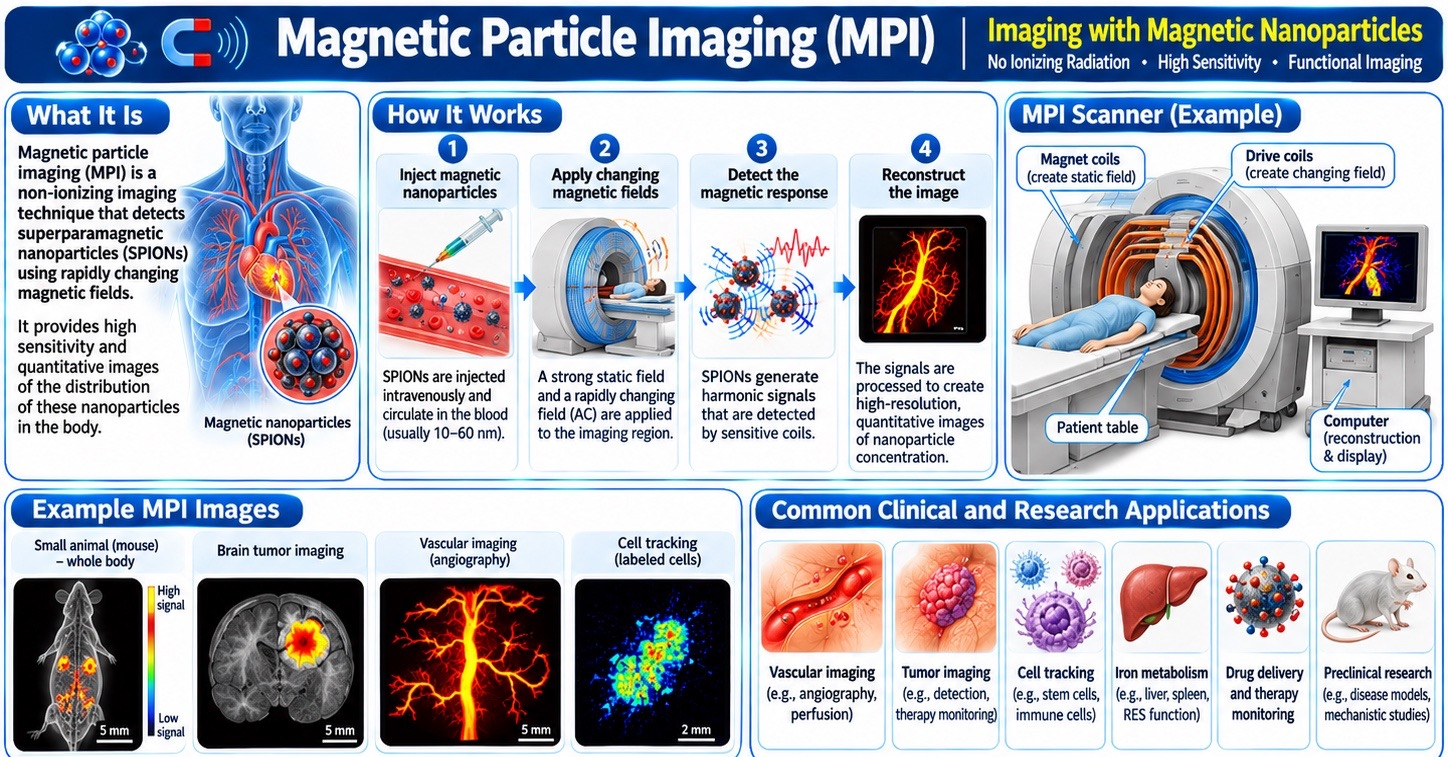
\includegraphics[width=\textwidth,height=0.6\textheight,keepaspectratio]{mpi.jpeg}
\end{center}
\noindent\textbf{Historical Context:} This earlier illustration is preserved for archival reference. It visually overstates clinical readiness---magnetic particle imaging (MPI) remains an investigational research modality with no FDA-approved clinical human scanner. For the current, medically vetted technical and safety summary of MPI, see Chapter~\ref{ch:infographic-mpi}.

\section{Why This Legacy Graphic Is Preserved}

Early promotional and conceptual illustrations of emerging medical technologies often depict compact, bedside, or routine hospital workflows long before full-scale human hardware, safety clearances, and approved tracers exist. Keeping this earlier MPI graphic alongside Chapter~\ref{ch:infographic-mpi} provides a concrete reminder of the gap between promising preclinical breakthroughs and routine clinical care.

\begin{itemize}
  \item \textbf{Current Clinical Status:} Invented in 2005, MPI has demonstrated impressive zero-background 3D tracking of superparamagnetic iron oxide nanoparticles (SPIONs) in small-animal scanners and early human-head research prototypes, but no clinical human MPI scanner is approved for routine diagnosis.
  \item \textbf{Key Translation Hurdles:} Scaling strong static magnetic gradients to full human-body size while staying within international peripheral nerve stimulation (PNS) and heating (SAR) limits, securing clinical approval for uniform MPI-optimized iron tracers, and pairing MPI with MRI or CT for anatomical context remain active areas of engineering research.
  \item \textbf{Standard Care Always Comes First:} Patients needing blood-vessel, stroke, bleeding, or cancer imaging today rely on established clinical modalities such as CT angiography (Chapter~\ref{ch:infographic-cta}), MRI/MRA (Chapters~\ref{ch:infographic-mri} and~\ref{ch:infographic-mra}), digital subtraction angiography (Chapter~\ref{ch:infographic-dsa}), or PET/CT (Chapter~\ref{ch:infographic-pet-ct}).
\end{itemize}

\section{Key References}
\begin{itemize}
  \item Gleich B, Weizenecker J. Tomographic imaging using the nonlinear response of magnetic particles. \textit{Nature}. 2005;435(7046):1214--1217.
  \item Graeser M, Thieben F, Szwargulski P, et al. Human-sized magnetic particle imaging for brain applications. \textit{Nature Communications}. 2019;10:1936.
  \item Talebloo N, Gudi M, Robertson N, Wang P. Magnetic particle imaging: current applications in biomedical research. \textit{Journal of Magnetic Resonance Imaging}. 2020;51(6):1659--1668.
  \item Harvell-Smith S, Tung LD, Thanh NTK. Magnetic particle imaging: tracer development and the biomedical applications of a radiation-free, sensitive, and quantitative imaging modality. \textit{Nanoscale} (NIH PubMed Central). 2022;14(10):3658--3697. Available at: \url{https://pmc.ncbi.nlm.nih.gov/articles/PMC8915192/}.
\end{itemize}

\section{Further Reading}
\begin{itemize}
  \item Wikipedia contributors. \textit{Magnetic particle imaging}. Wikipedia, The Free Encyclopedia. Available at: \url{https://en.wikipedia.org/wiki/Magnetic_particle_imaging}.
\end{itemize}


% --- Part III: Ultrasound Imaging Modalities ---
\part{Ultrasound Imaging Modalities}
\infographicchapter{Sound-Wave Imaging Modalities}{sound_cls..png}
\label{ch:infographic-sound-imaging-overview}

\section{Overview}

Sound-wave imaging---most commonly known as medical ultrasound (or sonography)---uses harmless, high-pitched sound waves that are too high for human ears to hear to see inside the body in real time. A small handheld wand (called a transducer) sends gentle pulses of sound into your body and listens for the echoes that bounce back off organs, fluid, and blood vessels. By timing how long each echo takes to return and how strong it is, the machine builds live moving pictures on a screen with zero ionizing radiation.

Beyond standard black-and-white ultrasound (B-mode) and motion tracking (M-mode), modern ultrasound includes several powerful specialized tools. Doppler ultrasound tracks the speed and direction of moving blood to check for narrowed arteries, leg blood clots (deep vein thrombosis), heart valve leaks, and blood flow to a developing baby. Ultrasound elastography gently measures how soft or stiff tissue is, helping check liver scarring (fibrosis) or evaluate breast and thyroid lumps. Contrast-enhanced ultrasound (CEUS) uses tiny, kidney-safe intravenous microbubbles to show blood flow inside liver or kidney spots without using X-ray dye. Doctors can also place tiny ultrasound probes inside scopes or heart catheters to look closely at deep organs.

Because ultrasound is safe, portable, painless, and works live at the bedside, it is an everyday cornerstone of pregnancy care, heart exams, abdominal scans, emergency trauma checks, and needle-guided biopsies. Its main limits are that image clarity depends on the skill of the person holding the probe, sound waves weaken in thicker tissue, and bone or air-filled lungs and bowel block sound echoes.

\section{Underlying Physical Principles}
\begin{itemize}
  \item \textbf{Harmless High-Frequency Sound Pulses:} Tiny crystals inside the handheld wand vibrate when given a small electrical pulse, sending safe high-frequency sound waves (2 to 18~megahertz) smoothly through soft tissue.
  \item \textbf{Echoes Map Organ Shapes and Depth:} Each tissue has a different resistance to sound, called \textit{acoustic impedance}. Whenever sound meets a boundary between tissues with different impedances (like fluid next to liver, or a hard gallstone), part of the sound bounces back as an echo---bigger mismatches create stronger, brighter echoes, while extreme mismatches like air or bone bounce nearly all the sound back. Clear fluid looks black, and the round-trip travel time tells the computer exactly how deep each structure sits.
  \item \textbf{Doppler Tracks Moving Blood:} Sound waves bouncing off moving red blood cells shift slightly in pitch (the Doppler effect), letting the scanner show blood-flow direction in color and measure blood speed accurately.
  \item \textbf{Measuring Stiffness and Tiny Microbubbles:} Elastography sends a gentle mechanical nudge into tissue and tracks tiny ripple waves---faster ripples mean stiffer tissue (such as liver scarring). In CEUS, safe microscopic gas bubbles injected into a vein vibrate softly in the sound beam, lighting up tiny blood vessels brightly.
  \item \textbf{Live Electronic Focusing:} The ultrasound machine steers and focuses its sound beam electronically many times per second, boosting deeper echoes and turning them smoothly into live 2D, 3D, Doppler, or stiffness pictures.
\end{itemize}

\section{Imaging Mechanism}
\begin{enumerate}
  \item \textbf{Picking the Probe and Applying Gel:} The sonographer picks the right handheld probe for your exam (lower-frequency probes see deeper into the belly or heart; higher-frequency probes give sharper views of the thyroid, breast, tendons, or blood vessels) and spreads warm or cool water-based gel on your skin to keep air out.
  \item \textbf{Sending Focused Sound Pulses:} The scanner sends rapid, harmless pulses of sound across the imaging area, smoothly switching between black-and-white anatomy, color Doppler blood flow, stiffness checks, or microbubble contrast views as needed.
  \item \textbf{Listening for Returning Echoes:} Returning echoes make the probe's crystals vibrate, creating tiny electrical signals that the machine amplifies (boosting fainter echoes from deeper organs) and converts into digital data.
  \item \textbf{Processing the Signal Live:} Fast processors sharpen the focus, smooth out grainy background speckle, and calculate blood-flow speeds or tissue stiffness numbers in real time.
  \item \textbf{Live Viewing and Saving:} Moving black-and-white videos, color blood-flow charts, stiffness maps, or contrast loops appear immediately on the bedside screen and are saved to your medical record for the doctor to interpret.
\end{enumerate}

\section{Key Technical Parameters}
\noindent
\begin{tabularx}{\textwidth}{@{}l X@{}}
\toprule
\textbf{Parameter} & \textbf{Typical Value / Description} \\
\midrule
Physical Principle & High-frequency sound pulses bounce off tissue boundaries, moving blood cells (Doppler), or tissue ripples (elastography) to build live images \\
Energy / Signal Source & Handheld or internal piezoelectric / micromachined ultrasound probes (transducers) \\
Typical Frequency / Energy & 2--5~MHz (deep belly, pregnancy, heart), 7--18~MHz (thyroid, breast, joints, veins), 20--40~MHz (inside heart arteries); kept within safe ALARA power limits \\
Spatial Resolution & About 0.3--1.5~mm detail depending on probe frequency and depth \\
Typical Scan Duration & 15--45~minutes for standard exams (2--5~minutes for rapid emergency FAST checks) \\
Contrast Agent & None for routine ultrasound, Doppler, or elastography; optional kidney-safe IV microbubbles for contrast-enhanced ultrasound (CEUS) \\
Ionizing Radiation & None (uses safe mechanical sound waves only) \\
\bottomrule
\end{tabularx}

\section{Clinical Usages}

\subsection{Primary Usages}
\begin{itemize}
  \item \textbf{Pregnancy and Pelvic Care:} Ultrasound is the safe, radiation-free first choice for confirming pregnancy, checking baby's growth and anatomy (including a routine scan commonly done between weeks 18 and 22, and optional 3D/4D views in the third trimester), checking amniotic fluid, the placenta, and umbilical blood flow, guiding prenatal tests like amniocentesis and chorionic villus sampling (CVS), and evaluating pelvic pain, ovarian cysts, or fibroids.
  \item \textbf{Heart and Blood-Vessel Checks:} Heart ultrasound (echocardiography) checks pumping strength, heart valves, and fluid around the heart. Vascular Doppler checks for leg blood clots (deep vein thrombosis) and narrowed neck or leg arteries.
  \item \textbf{Belly, Gallbladder, and Kidney Scans:} Ultrasound is usually the first test ordered for gallstones, gallbladder inflammation, blocked kidneys, liver enlargement, abdominal fluid, and screening for abdominal aortic aneurysms.
  \item \textbf{Emergency Checks and Needle Guidance:} Rapid bedside trauma exams (FAST), lung checks, and live needle guidance make biopsies, fluid drainages, and IV line placements faster and safer.
  \item \textbf{Thyroid, Breast, Joint, and Infant Scans:} High-frequency probes give sharp first-line views of thyroid nodules, breast cysts and lumps (especially in younger women or dense breasts), testicular pain, torn tendons, and the brain, spine, and hips in infants.
\end{itemize}

\subsection{Secondary Usages}
\begin{itemize}
  \item \textbf{Measuring Tissue Stiffness (Elastography):} Shear-wave and strain elastography gently measure liver scarring (fibrosis) without a biopsy and help sort breast, thyroid, and prostate lumps.
  \item \textbf{Microbubble Contrast Scans (CEUS):} Kidney-safe IV microbubbles help doctors tell harmless liver or kidney spots from tumors and check for leaks around repaired aortic stents without X-rays or kidney-stressing CT dye.
  \item \textbf{Internal Scope and Artery Ultrasound:} Endoscopic ultrasound (EUS) and intravascular ultrasound (IVUS) bring tiny high-resolution probes right next to the pancreas, digestive wall, or inside heart arteries for detailed staging.
  \item \textbf{Focused Ultrasound Treatments:} High-intensity focused ultrasound (HIFU) treats uterine fibroids, essential tremor, and select prostate lesions without cuts, while gentler focused ultrasound is being studied to help medicines cross into the brain.
\end{itemize}

\section{Advantages}
\begin{itemize}
  \item \textbf{Zero Ionizing Radiation:} Harmless sound waves make ultrasound the safest first-line scan for pregnancy, children, and frequent follow-up checkups.
  \item \textbf{Live Moving Pictures:} High-speed live video shows beating heart valves, flowing blood, and exact needle tips in real time during biopsies or drainages.
  \item \textbf{Portable, Fast, and Affordable:} Compact bedside and handheld scanners deliver quick answers in clinics, emergency rooms, ICUs, and rural settings at much lower cost than CT or MRI.
  \item \textbf{Many Built-In Capabilities:} One ultrasound machine can combine standard anatomy, Doppler blood flow, stiffness elastography, and kidney-safe microbubble contrast.
  \item \textbf{Comfortable and Widely Safe:} Exams are open-air, quiet, and completely safe for people with claustrophobia, pacemakers, metal implants, or severe kidney disease.
\end{itemize}

\section{Disadvantages}
\begin{itemize}
  \item \textbf{Depends on Operator Skill:} Getting clear, accurate images relies heavily on the training, experience, and careful probe handling of the sonographer or doctor.
  \item \textbf{Blocked by Bone and Air:} Hard bone and air-filled lungs or bowel bounce sound away and cast dark shadows, limiting views of the adult brain or deep areas behind bowel gas.
  \item \textbf{Harder to See Through Thicker Tissue:} In larger patients, sound waves weaken over longer distances, requiring lower-frequency probes that produce slightly less sharp pictures.
  \item \textbf{Narrow View and Echo Glitches:} Ultrasound looks through a small window at a time rather than showing the whole body at once, and bouncing sound can occasionally create mirror or shadow artifacts.
  \item \textbf{Gentle Output Limits:} Although very safe, prolonged high-power Doppler requires keeping acoustic warmth (Thermal Index, TI) and vibration (Mechanical Index, MI) low, especially in early pregnancy and eye exams.
\end{itemize}

\section{Patient Safety Guidelines}
\begin{itemize}
  \item \textbf{Keeping Sound Energy Low (ALARA):} Operators follow AIUM and FDA safety rules by keeping scan time brief and keeping Thermal Index (TI) and Mechanical Index (MI) as low as possible---especially during early-pregnancy Doppler, newborn brain scans, and eye scans.
  \item \textbf{Clean Probes and Sterile Gel:} Probes are wiped clean with disinfectant after skin exams. Internal probes (vaginal, rectal, throat) and probes used on open skin or during biopsies undergo high-level disinfection and wear single-use sterile covers with sterile gel packets.
  \item \textbf{Microbubble Contrast Safety (CEUS):} Staff check for contrast allergies, take extra care in unstable heart or lung disease, and keep emergency allergy treatment ready for rare reactions.
  \item \textbf{Medical Use Only and Equipment Checks:} Medical groups advise against non-medical commercial ``keepsake'' baby ultrasounds. Staff regularly inspect probes and cords for cracks or warmth, and use strict sterile technique during needle procedures.
\end{itemize}

\section{Augmenting Methods}
\begin{itemize}
  \item \textbf{Contrast CT and MRI:} CT and MRI see right past bone, bowel gas, and thicker tissue to stage cancers and clarify uncertain liver, kidney, or pelvic findings.
  \item \textbf{Nuclear Medicine Scans (HIDA, V/Q, PET/CT):} A HIDA scan settles uncertain gallbladder inflammation, while PET/CT and thyroid nuclear scans add functional detail to ultrasound findings.
  \item \textbf{Built-In Ultrasound Add-Ons:} Combining regular B-mode views with Doppler blood flow, shear-wave elastography, and kidney-safe CEUS greatly boosts accuracy right at the bedside.
  \item \textbf{Blood Tests:} Simple labs---like a pregnancy test (beta-hCG), D-dimer for blood clots, liver panels, or thyroid TSH---help doctors interpret ultrasound findings accurately.
  \item \textbf{Ultrasound-Guided Biopsy and AI Helpers:} Live needle guidance makes tissue biopsies safe and exact, while new AI tools help guide probe angles and measure baby or heart sizes more consistently.
\end{itemize}

\section{Comparison with Alternative Modalities}
\begin{itemize}
  \item \textbf{Versus CT:} Ultrasound is radiation-free, portable, less costly, and guides needles live, while CT does not depend on operator skill, sees right through bone and bowel gas, and is better for whole-body trauma and cancer staging.
  \item \textbf{Versus MRI:} Ultrasound is much faster, quieter, bedside-ready, and safe with any metal implant, while MRI gives broader, deeper soft-tissue detail for the brain, spine, and pelvis.
  \item \textbf{Versus Nuclear Medicine:} Ultrasound quickly shows gallstones, blocked kidneys, and surface lumps structurally, while nuclear medicine excels at whole-organ function and whole-body cancer metabolism.
  \item \textbf{Versus Optical Scans:} Ultrasound sees many centimeters deep into organs and blood-filled vessels, while optical tools like OCT see finer microscopic detail only within the top few millimeters.
\end{itemize}

\section{Key References}
\begin{itemize}
  \item American Institute of Ultrasound in Medicine (AIUM). \textit{AIUM Official Statements and Practice Parameters for the Performance of Diagnostic Ultrasound Examinations}. Laurel, MD: AIUM, 2024.
  \item Rumack CM, Levine D. \textit{Diagnostic Ultrasound}. 6th ed. Philadelphia, PA: Elsevier, 2023.
  \item Dietrich CF, Nolsoe CP, Barr RG, et al. Guidelines and good clinical practice recommendations for contrast-enhanced ultrasound (CEUS) in the liver --- update 2020. \textit{Ultrasound in Medicine \& Biology}. 2020;46(10):2579--2604.
  \item Barr RG, Wilson SR, Rubens D, Garcia-Tsao G, Ferraioli G. Update to the Society of Radiologists in Ultrasound liver elastography consensus statement. \textit{Radiology}. 2020;296(2):263--274.
  \item National Library of Medicine (MedlinePlus). \textit{Ultrasound}. National Institutes of Health. Available at: \url{https://medlineplus.gov/lab-tests/sonogram/}.
  \item Radiopaedia.org. \textit{Ultrasound (introduction)}. Radiopaedia. Available at: \url{https://radiopaedia.org/articles/ultrasound-introduction}.
\end{itemize}

\section{Further Reading}
\begin{itemize}
  \item Wikipedia contributors. \textit{Medical ultrasound}. Wikipedia, The Free Encyclopedia. Available at: \url{https://en.wikipedia.org/wiki/Medical_ultrasound}.
\end{itemize}

\infographicchapter{Ultrasound}{ultrasound.png}
\label{ch:infographic-ultrasound}

\section{Overview}

Diagnostic ultrasound---also called sonography---is one of the safest, most familiar, and most versatile medical imaging tests in healthcare. Instead of X-rays, it uses gentle, high-frequency sound waves (between 2 and 18 MHz, far above human hearing) to create live, moving pictures of organs, soft tissues, and blood flow inside your body. A small handheld probe glides over warm or cool water-based gel on your skin, sending sound pulses inward and listening to the echoes that bounce back from different tissues. A computer turns those echoes into real-time black-and-white images, while special Doppler modes measure blood flow speed and direction.

Because ultrasound works across almost every part of the body, doctors choose the probe frequency to match the depth they need. Lower-frequency probes (2--5 MHz) reach deeper for pregnancy checkups, pelvic exams, liver, gallbladder, kidney, and abdominal scans, and heart ultrasounds (echocardiograms). Higher-frequency probes (7--18 MHz) create crisp close-up views of areas near the skin---including the thyroid, breast, scrotum, neck and leg blood vessels, and joints or tendons---and also guide doctors safely during needle biopsies or fluid drainages.

Ultrasound's biggest advantages are zero X-ray radiation, painless noninvasive scanning, live motion viewing, bedside portability, affordability, and an exceptional ability to tell harmless fluid-filled cysts apart from solid lumps. Its main limits are that picture quality depends strongly on the examiner's skill, it looks at one smaller area at a time rather than the whole body, thick tissue layers can soften deep views, and sound waves cannot travel well through air (such as lungs or bowel gas) or dense bone. Diagnostic ultrasound has an outstanding safety record, and clinicians always keep sound energy as low as reasonably achievable (ALARA), especially during pregnancy and Doppler scans.

\section{Underlying Physical Principles}

\begin{itemize}
    \item \textbf{Sound-Making Crystals in the Probe:} Inside the handheld probe sit tiny piezoelectric crystals. When a brief electrical pulse hits them, they vibrate to send out high-frequency sound waves (2--18 MHz). When returning echoes bounce back from your body, those same crystals vibrate again and turn the echoes back into electrical signals.
    \item \textbf{How Echoes Create Shades of Gray (Echogenicity):} Tissues bounce sound differently based on their \textit{acoustic impedance} (how strongly a material resists sound waves). Sharp boundaries---like soft tissue meeting air or hard bone---reflect nearly all sound back, casting a dark shadow. Smooth fluid (like urine, bile, or a simple cyst) lets sound pass right through and looks black (\textit{anechoic}) with bright tissue behind it; soft organs appear gray (\textit{hypoechoic} if darker, \textit{isoechoic} if matching nearby tissue), while dense stones, fat interfaces, or bone appear bright white (\textit{hyperechoic}).
    \item \textbf{Timing Depth and Focusing the Beam:} The probe's electronics focus and steer the sound beam smoothly across the target area. By timing how long each echo takes to return, the computer knows exactly how deep each structure sits, and automatically boosts faint echoes from deeper organs so the picture looks evenly bright.
    \item \textbf{Measuring Blood Flow With the Doppler Effect:} Just as an ambulance siren changes pitch as it drives past, sound waves bouncing off moving red blood cells shift slightly in frequency. Color Doppler paints blood flow direction onto the screen, while spectral Doppler graphs exact blood speed to spot narrowed arteries or clots.
    \item \textbf{Imaging Modes and Advanced Features:} Standard live 2D grayscale scanning is called \textit{B-mode} (brightness mode), whereas \textit{M-mode} (motion mode) tracks rapid movement along a single line over time---ideal for timing heart valves or a baby's heartbeat. Modern scanners also provide 3D/4D surface views, tissue harmonic imaging for cleaner pictures, elastography to measure tissue stiffness (such as liver scarring), and contrast-enhanced ultrasound (CEUS) using tiny harmless gas microbubbles to highlight fine blood flow.
\end{itemize}

\section{Imaging Mechanism}

\begin{enumerate}
    \item \textbf{Choosing the Probe and Applying Gel:} The sonographer picks a probe shaped and tuned for your exam---curved for the abdomen, flat and high-frequency for shallow areas like the thyroid or breast, or specialized for the heart or pelvis---and applies water-based gel (or a sterile cover and sterile gel for internal or needle-guided exams) to remove air gaps.
    \item \textbf{Sweeping the Sound Beam:} The scanner fires rapid, precisely timed sound pulses across the target area while the sonographer glides and tilts the probe, switching smoothly between black-and-white anatomy views, color blood-flow Doppler, or stiffness modes as needed.
    \item \textbf{Listening to Returning Echoes:} Returning echoes vibrate the probe's crystals into tiny electrical signals, which are boosted, balanced for depth, and converted into digital data.
    \item \textbf{Building Live Pictures and Flow Graphs:} The computer cleans up speckle noise, sharpens tissue edges, and calculates live blood-flow colors, velocity graphs, or stiffness maps in real time.
    \item \textbf{Viewing, Measuring, and Saving:} Live moving pictures appear immediately on the screen alongside safety gauges. The sonographer measures key structures and saves still images and short video clips for the radiologist to interpret.
\end{enumerate}

\section{Key Technical Parameters}

\noindent
\begin{tabularx}{\textwidth}{@{}l X@{}}
\toprule
\textbf{Parameter} & \textbf{Typical Value / Description} \\
\midrule
Physical Principle & Pulse-echo reflection of high-frequency sound waves at tissue boundaries, plus Doppler blood-flow and stiffness modes \\
Energy / Signal Source & Handheld piezoelectric ultrasound probe (curved, flat linear, heart phased-array, or internal) \\
Typical Frequency / Energy & 2--5 MHz (abdomen, pelvis, pregnancy, heart) and 7--18 MHz (thyroid, breast, scrotum, blood vessels, joints/tendons) \\
Spatial Resolution & About 0.2--1.5 mm (finer detail with high-frequency shallow probes) \\
Typical Scan Duration & 15--45 minutes \\
Contrast Agent & None routinely; optional intravenous microbubble contrast for specialized CEUS exams \\
Ionizing Radiation & None (0 mSv) \\
\bottomrule
\end{tabularx}

\section{Common Symptoms That Prompt This Scan}
\begin{itemize}
    \item \textbf{Belly, Side, or Pelvic Pain:} Upper-right pain after fatty meals (gallstones), lower-belly or pelvic cramping, bloating, or flank pain pointing to kidney swelling or stones.
    \item \textbf{A New Neck, Groin, or Soft-Tissue Lump:} A painless or tender swelling in the thyroid, neck, armpit, groin, or under the skin to quickly tell fluid cysts from solid lumps.
    \item \textbf{Pregnancy Checkups and Pelvic Symptoms:} Routine prenatal monitoring, pelvic pain, or abnormal vaginal bleeding without any X-ray radiation.
    \item \textbf{Testicular or Scrotal Pain and Swelling:} Sudden or gradual scrotal aching, heaviness, or a noticeable lump needing prompt, painless evaluation.
\end{itemize}

\section{Clinical Usages}

\subsection{Primary Usages}

\begin{itemize}
    \item \textbf{Pregnancy and Women's Health:} The go-to first exam for confirming pregnancy, checking due dates, monitoring baby growth and anatomy (with a routine detailed check commonly performed between weeks 18 and 22), checking the placenta and amniotic fluid, guiding prenatal sampling such as amniocentesis or chorionic villus sampling (CVS), and evaluating ectopic pregnancy, uterine fibroids, ovarian cysts, or pelvic pain.
    \item \textbf{Abdomen, Liver, and Kidneys:} The first-choice test for gallstones, gallbladder inflammation, blocked bile ducts, fatty liver or liver spots, swollen kidneys, kidney masses, and screening for an enlarged abdominal aorta (aneurysm).
    \item \textbf{Blood Vessels and Clots:} Checking leg or arm veins for blood clots (deep vein thrombosis), screening neck (carotid) arteries for narrowing, checking leg circulation, and verifying blood flow in transplanted organs.
    \item \textbf{Shallow Organs, Prostate, and Children:} Evaluating thyroid and parathyroid nodules, breast lumps (telling fluid cysts apart from solid lumps, especially in younger or dense breasts), sudden scrotal pain (testicular torsion or infection), the prostate gland (via transrectal ultrasound), and childhood conditions like pyloric stenosis, intussusception, or infant hip, brain, and spine development.
    \item \textbf{Heart Ultrasound (Echocardiography):} Checking heart chamber size, pumping strength, leaky or stiff heart valves, fluid around the heart, and congenital heart conditions---either across the chest wall or via a specialized probe in the esophagus (transesophageal echocardiogram, or TEE) for closer views.
\end{itemize}

\subsection{Secondary Usages}

\begin{itemize}
    \item \textbf{Live Needle Guidance:} Guiding needle biopsies (thyroid, breast, liver, lymph nodes), fluid drainages from the chest or abdomen, abscess drains, joint injections, and tricky IV placements in real time.
    \item \textbf{Joints, Tendons, and Muscles:} Checking rotator cuff tears, tendon inflammation, bursitis, ligament sprains, pinched nerves (like carpal tunnel syndrome), and surface lumps while you move the joint.
    \item \textbf{Tissue Stiffness Checks (Elastography):} Measuring liver stiffness to check for scarring without a biopsy, and adding stiffness clues for breast or thyroid nodules.
    \item \textbf{Contrast-Enhanced Ultrasound (CEUS):} Using tiny, kidney-safe gas microbubbles to clarify liver or kidney spots and check aortic stent grafts for leaks without X-ray radiation.
\end{itemize}

\section{Advantages}

\begin{itemize}
    \item \textbf{Zero Radiation and Proven Safety:} Uses gentle sound waves rather than X-rays, making it the safest first-line scan during pregnancy, for children, and for repeat follow-ups.
    \item \textbf{Live Motion and Blood Flow:} Shows organs moving in real time---like a beating heart, a moving baby, or gliding tendons---measures blood flow with Doppler, and guides needles safely.
    \item \textbf{Clearly Separates Cysts From Solid Lumps:} Reliably tells harmless fluid-filled cysts apart from solid or complex masses in the breast, thyroid, ovaries, kidneys, and liver.
    \item \textbf{Widely Available, Portable, and Affordable:} Costs far less than CT or MRI, is available almost everywhere, and portable machines can roll right to a hospital bedside or emergency room.
    \item \textbf{Noninvasive and Usually Dye-Free:} Most scans need no IV line or contrast dye; when microbubble contrast is used, it is breathed out through the lungs and is safe for the kidneys.
\end{itemize}

\section{Disadvantages}

\begin{itemize}
    \item \textbf{Depends Strongly on Examiner Skill:} Picture quality and accuracy rely heavily on the sonographer's technique in positioning the probe and tuning the settings, so results can vary more between operators than automated CT or MRI scans.
    \item \textbf{Blocked by Air, Bone, and Deep Tissue Layers:} Sound bounces off air and bone, making it hard to image air-filled lungs, the adult brain, organs hidden behind bowel gas, or areas behind thick bone. Heavy body weight can also soften deep images.
    \item \textbf{Smaller Viewing Window and Echo Tricks:} Shows one smaller region at a time rather than a whole-body overview, and harmless echo illusions (like shadowing or mirror images) can occasionally mimic real findings.
    \item \textbf{Keeping Sound Energy Gentle:} High sound power---especially prolonged pulsed Doppler in early pregnancy---can cause slight local warming, so clinicians strictly follow ALARA safety limits.
    \item \textbf{Not Right for Every Question:} Cannot replace CT or MRI for full-body cancer staging, sudden brain bleeding, complex bone fractures, or deep lung disease.
\end{itemize}

\section{Contraindications}

\subsection{Absolute}

\begin{itemize}
    \item \textbf{None for Routine Skin-Surface Ultrasound:} Standard grayscale and Doppler ultrasound over intact skin has no strict medical contraindications.
    \item \textbf{Allergy to Microbubble Contrast (CEUS Only):} Intravenous microbubble contrast must not be used if you have a known allergy to the microbubble agent.
\end{itemize}

\subsection{Relative}

\begin{itemize}
    \item \textbf{Internal Scans and Open Wounds:} Internal (transvaginal or transrectal) scans are avoided if there is a severe local blockage, very recent pelvic or rectal surgery, or if a patient declines. Scanning over open wounds or fresh incisions uses a sterile probe cover and sterile gel.
    \item \textbf{Biopsies and Contrast Precautions:} Uncorrected severe bleeding disorders are a caution before ultrasound-guided needle biopsies or deep drainages, and severe unstable heart or lung conditions warrant extra care before microbubble contrast.
\end{itemize}

\section{Patient Safety Guidelines}

\begin{itemize}
    \item \textbf{ALARA Safety Limits and Medical Need:} Following AIUM and WFUMB guidelines, sonographers use the lowest sound power and shortest scan time needed, watching on-screen Thermal Index (TI) and Mechanical Index (MI) gauges---especially in early pregnancy, pulsed Doppler, and eye scans (TI at or below 1.0, MI at or below 0.23). Because sound energy can subtly affect body fluids and tissues under certain conditions, medical experts recommend using ultrasound only when needed to provide important health information.
    \item \textbf{Probe Cleaning and Infection Control:} Probes and cords are wiped with disinfectant between every routine skin scan. Internal probes, scans over broken skin, and needle-guided procedures require high-level disinfection plus a fresh sterile cover and single-use sterile gel.
    \item \textbf{Microbubble Contrast Safety (CEUS):} Before CEUS, staff check for allergies and heart-lung stability, use low-energy contrast settings, and keep emergency care supplies nearby.
    \item \textbf{Equipment Checks:} Staff inspect probe faces and cables before each scan for cracks or overheating to keep you safe from electrical or heat irritation.
    \item \textbf{Comfort in Late Pregnancy and Needle Safety:} In mid-to-late pregnancy, lying slightly tilted on your left side avoids pressure on major abdominal blood vessels. During biopsies, the clinician watches the needle tip continuously on screen.
\end{itemize}

\section{Prerequisite Tests}

\begin{itemize}
    \item \textbf{No Routine Blood Tests for Standard Scans:} Regular grayscale and Doppler ultrasounds are noninvasive and dye-free, so no blood work is needed beforehand.
    \item \textbf{Simple Exam-Specific Prep:} Check your appointment instructions---abdominal and gallbladder scans usually require 6--8 hours of fasting, while pelvic and early pregnancy scans often ask for a comfortably full bladder.
    \item \textbf{Pregnancy Test (When Helpful):} For pelvic pain or unusual bleeding in patients who could be pregnant, a quick urine or blood pregnancy test helps the team tailor the scan and interpret early pregnancy findings.
    \item \textbf{Blood-Clotting Checks (For Biopsies Only):} Before an ultrasound-guided needle biopsy or deep fluid drainage, your doctor reviews blood clotting tests (INR and platelets) and any blood-thinning medicines.
    \item \textbf{Allergy and Heart-Lung Check (For CEUS Only):} Before microbubble contrast, staff check for past reactions and heart-lung stability; no kidney blood test is needed because the gas is breathed out through the lungs.
\end{itemize}

\section{Preparing for the Scan}

\begin{itemize}
    \item \textbf{Fasting for Abdomen and Gallbladder Scans:} For liver, gallbladder, pancreas, or abdominal aorta scans, avoid food, fizzy drinks, and chewing gum for 6--8 hours beforehand so the gallbladder stays full and bowel gas stays low. Small sips of plain water with essential pills are usually fine.
    \item \textbf{Full Bladder for Pelvic and Early Pregnancy Scans:} For lower-belly pelvic, bladder, or early pregnancy scans, drink about 24--32 ounces (700--950 mL) of water finishing 45--60 minutes before your visit and do not empty your bladder, as a full bladder acts like a clear window. (If an internal transvaginal scan is planned, you will empty your bladder right before that part.)
    \item \textbf{Little to No Prep for Shallow or Blood-Vessel Scans:} Thyroid, breast, scrotal, joint, neck artery, and leg vein scans need no fasting or full bladder---just skip thick lotions, oils, or powders on the area being scanned.
    \item \textbf{Easy-Access Clothing:} Wear loose, comfortable two-piece clothing so the area can be uncovered easily, and remove necklaces or jewelry near the scan site.
    \item \textbf{Biopsy or Contrast Prep:} If you are scheduled for a needle biopsy, drainage, or microbubble contrast scan, follow your clinic's specific instructions on blood thinners, fasting if sedation is planned, IV placement, and having a ride home.
\end{itemize}

\section{During Scan}

\begin{itemize}
    \item \textbf{Comfortable Positioning:} You lie on a padded exam bed---usually on your back, turning slightly onto your side, or sitting upright depending on the body part (with a gentle left-side tilt in late pregnancy)---and stay relaxed while the sonographer glides the probe.
    \item \textbf{Simple Breathing Cues:} You breathe normally for most of the exam. For liver, gallbladder, or kidney views, the sonographer may ask you to take a deep breath and hold it for 5--10 seconds so the organs drop below your ribs for a clearer view.
    \item \textbf{What You Will Feel and Hear:} You will feel cool or warmed gel on your skin and gentle-to-firm gliding pressure from the smooth probe (which can feel briefly snug over a full bladder or sore spot). During Doppler checks, you may hear a gentle rhythmic whooshing sound of your blood flow.
    \item \textbf{Speak Up Anytime:} The sonographer stays right beside you the entire time. Tell them immediately if probe pressure hurts, if lying flat makes you dizzy or short of breath, or if your full bladder feels painfully tight.
    \item \textbf{Time and Pacing:} Most diagnostic ultrasounds take 15--45 minutes depending on how many areas and blood-flow checks are needed, with zero recovery time afterward for standard scans.
\end{itemize}

\section{Normal Appearance}

\begin{itemize}
    \item \textbf{Smooth, Even Solid Organs:} A healthy liver, spleen, thyroid, or testicle looks smooth, finely speckled, and even in shade with neat outer borders and no lumps or hard shadows.
    \item \textbf{Clean Fluid Spaces:} A fasting gallbladder appears as a thin-walled, pear-shaped black sac without bright stones or surrounding fluid, and the bladder fills cleanly with clear black urine.
    \item \textbf{Healthy Kidneys and Blood Vessels:} Normal kidneys show smooth outer tissue and a bright center without backed-up fluid. Healthy veins flatten easily under gentle probe pressure, and arteries show smooth, steady blood-flow waves.
    \item \textbf{Healthy Tendons and Pregnancy:} Healthy tendons show neat, bright parallel fibers, while a normal early pregnancy shows an appropriately sized sac, expected baby growth, healthy fluid levels, and a regular heartbeat.
\end{itemize}

\section{Observing for Abnormal Patterns}

\begin{itemize}
    \item \textbf{Simple Fluid-Filled Cysts:} A smooth, round, completely black spot with a bright glow directly behind it is the classic sign of a harmless fluid-filled cyst in the kidney, liver, breast, thyroid, or ovary.
    \item \textbf{Bright Stones and Gallbladder Inflammation:} Bright white spots casting a sharp dark shadow behind them identify gallstones, kidney stones, or hard calcium deposits. A thickened gallbladder wall (over 3 mm), fluid around it, and tenderness under the probe point to acute gallbladder inflammation (cholecystitis).
    \item \textbf{Suspicious Solid Lumps and Fatty Liver:} Jagged, taller-than-wide dark solid nodules with tiny bright calcium specks or tangled internal blood flow raise concern for cancer in the breast or thyroid. An unusually bright liver that dims deeper views points to fatty liver (hepatic steatosis).
    \item \textbf{Blood-Flow Problems on Doppler:} A vein that will not flatten under gentle pressure and lacks blood flow confirms a blood clot (DVT). Very fast, turbulent blood flow pinpoints a narrowed artery (such as in the neck), while missing blood flow in a painful testicle or ovary flags urgent twisting (torsion).
    \item \textbf{Common Echo Illusions:} Bowel gas or surgical clips can create bright repeating streaks, reflections off the diaphragm can mirror a liver spot into the chest, and faint echo blur can make a clear cyst look like it has debris inside unless checked from another angle.
\end{itemize}

\section{Dealing with Uncertainties}

\begin{itemize}
    \item \textbf{Gas, Bone, and Deep-Tissue Barriers:} Heavy body weight softens deep sound waves, and overlying bowel gas, lungs, or ribs can block views of the pancreas, deep pelvis, or abdominal aorta.
    \item \textbf{Technique and Echo Illusions:} Image clarity depends strongly on probe angle, frequency choice, and settings; echo artifacts can sometimes mimic debris inside cysts or exaggerate artery narrowing.
    \item \textbf{Prep Challenges:} An empty bladder during a pelvic scan or a shrunk gallbladder after a recent meal can make the view unreadable or falsely look like a thickened gallbladder wall.
    \item \textbf{Borderline Lumps:} Some complex cysts, liver or kidney spots, or thyroid and ovarian nodules share features of both harmless and serious conditions, so standard ultrasound alone cannot always give a final answer.
    \item \textbf{What Normal and Abnormal Results Mean:} Even a normal ultrasound cannot detect every condition or birth defect, and an unusual finding does not automatically mean a serious health problem---your doctor may recommend follow-up imaging or extra tests to confirm.
    \item \textbf{How Doctors Clarify Results:} Clinics may repeat a scan after proper fasting or drinking water, shift your position or try a different probe angle, add Doppler, stiffness checks (elastography), or microbubble contrast (CEUS), or recommend CT, MRI, a follow-up check, or a quick needle biopsy.
\end{itemize}

\section{Augmenting Methods}

\begin{itemize}
    \item \textbf{Contrast-Enhanced Ultrasound (CEUS) and Elastography:} Microbubble contrast clarifies liver and kidney spots in real time without harming the kidneys, while elastography measures liver scarring or lump stiffness.
    \item \textbf{CT and MRI Scans:} Overcome bowel gas, bone, and deep-tissue limits to give wide-angle 3D views for cancer staging, pancreatic disease, and detailed soft-tissue checks.
    \item \textbf{Ultrasound-Guided Needle Biopsy:} Uses live ultrasound guidance to take a tiny, accurate tissue sample from uncertain thyroid, breast, liver, or lymph node spots with minimal discomfort.
    \item \textbf{Targeted Blood Tests:} Pairing ultrasound with pregnancy hormones (beta-hCG), liver tests, blood-clot checks (D-dimer), PSA, or CA-125 sharpens the diagnosis.
    \item \textbf{Standardized Risk Scores and AI Support:} Clear scoring systems (BI-RADS for breast, TI-RADS for thyroid, LI-RADS for liver, O-RADS for ovaries) and modern AI measurement tools keep reporting consistent and evidence-based.
\end{itemize}

\section{Comparison with Alternative Modalities}

\begin{itemize}
    \item \textbf{Versus CT Scan:} CT gives wide, rapid 3D views unaffected by bowel gas or body size (better for major trauma and cancer staging), while ultrasound uses zero radiation and no kidney-stressing dye and shines for pregnancy, gallstones, blood clots, and shallow organs.
    \item \textbf{Versus MRI:} MRI gives unmatched deep soft-tissue detail (for brain, spine, or complex liver and pelvic masses), while ultrasound is much faster, far less expensive, widely available, and ideal for live motion and needle guidance.
    \item \textbf{Versus Bedside Quick Scans (POCUS):} Focused bedside ultrasound answers urgent, single questions in seconds during emergencies, whereas a full diagnostic ultrasound provides thorough multi-organ views, detailed Doppler measurements, and formal radiology reporting.
\end{itemize}

\section{Follow-up Steps}

\begin{itemize}
    \item \textbf{Right After the Exam:} Standard diagnostic ultrasound needs zero recovery time---wipe off the gel and go right back to your day. After microbubble contrast (CEUS), you may rest briefly for observation; after a biopsy or drainage, staff monitor your vital signs and puncture site briefly before you head home.
    \item \textbf{Clear Reporting and Urgent Alerts:} Radiologists use standardized scoring systems (BI-RADS, TI-RADS, O-RADS, LI-RADS) and call your doctor immediately if an urgent finding---like a blood clot, ectopic pregnancy, torsion, or leaking aneurysm---needs fast care.
    \item \textbf{Next-Step Imaging or Biopsy:} If a scan is limited by gas or shows a borderline spot, your doctor may order a targeted CT, MRI, or a simple ultrasound-guided needle biopsy for a definitive answer.
    \item \textbf{Routine Checkups Over Time:} For harmless or low-risk findings, your doctor may simply schedule a follow-up ultrasound---such as tracking a small abdominal aneurysm, rechecking a thyroid nodule or ovarian cyst, or monitoring baby growth in later pregnancy.
\end{itemize}

\section{Key References}

\begin{itemize}
    \item American Institute of Ultrasound in Medicine (AIUM) and American College of Radiology (ACR). \textit{AIUM--ACR--SPR--SRU Practice Parameters for Diagnostic Ultrasound Examinations}.
    \item World Federation for Ultrasound in Medicine and Biology (WFUMB). \textit{Safety Guidelines for Diagnostic Ultrasound, Elastography, and Contrast-Enhanced Ultrasound}.
    \item Rumack CM, Levine D. \textit{Diagnostic Ultrasound}, 5th ed. Philadelphia: Elsevier.
    \item Carovac A, Smajlovic F, Junuzovic D. Application of ultrasound in medicine. \textit{Acta Informatica Medica}. 2011;19(3):168--171.
    \item National Library of Medicine (MedlinePlus). \textit{Ultrasound: MedlinePlus Medical Test}. National Institutes of Health. Available at: \url{https://medlineplus.gov/lab-tests/sonogram/}.
    \item Radiopaedia.org. \textit{Ultrasound (introduction)}. Radiopaedia. Available at: \url{https://radiopaedia.org/articles/ultrasound-introduction}.
\end{itemize}

\section{Further Reading}
\begin{itemize}
  \item Wikipedia contributors. \textit{Medical ultrasound}. Wikipedia, The Free Encyclopedia. Available at: \url{https://en.wikipedia.org/wiki/Medical_ultrasound}.
\end{itemize}

\infographicchapter{Doppler Ultrasound}{doppler_ultrasound.png}
\label{ch:infographic-doppler-ultrasound}

\section{Overview}

Doppler ultrasound is a safe, noninvasive ultrasound exam that watches blood moving through your arteries and veins in real time. While a standard ultrasound shows the shape of your organs and blood vessels, Doppler ultrasound adds sound-wave tracking of blood flow speed and direction. It works by the same Doppler effect that makes a passing ambulance siren change pitch: when gentle, high-frequency sound waves bounce off moving red blood cells, the pitch of the returning echo shifts depending on how fast and which way the blood is flowing. Depending on the question, the scanner can show flow as red and blue colors over the vessel (color Doppler), as a detailed speed graph over time (spectral Doppler), or as a sensitive glow that picks up very slow flow (power Doppler). When standard black-and-white anatomy pictures are paired with Doppler flow, the exam is often called a \textbf{duplex} (or \textbf{triplex}) ultrasound on clinic orders. Unlike textbook diagrams, the red and blue colors do not mean arteries versus veins---by convention, red shows blood flowing toward the probe and blue shows blood flowing away, with brighter shades marking faster flow.

By pairing live anatomy with blood-flow measurements---such as peak flow speed and how easily blood flows through downstream organs---Doppler ultrasound spots narrowed arteries, blood clots in veins, swirling turbulence, and reduced blood supply to organs. Doctors commonly order it to check for leg or arm blood clots (deep vein thrombosis, or DVT), measure narrowing in neck (carotid) or leg arteries, check heart valves, monitor blood flow between mother and baby during pregnancy, rule out painful twisting of a testicle or ovary (torsion), monitor transplanted organs, and check brain blood vessels.

Doppler ultrasound uses no X-ray radiation and no kidney-stressing contrast dye, is portable enough to bring to a hospital bedside, and costs far less than CT or MRI. Its main limits are that accurate speed readings require angling the probe properly along the vessel (below 60 degrees, because sound waves hitting a vessel straight-on at 90 degrees cannot measure flow speed), very fast blood flow can wrap around on the graph (aliasing), results depend strongly on the sonographer's skill, and deep body tissue, bowel gas, or thick bone can block the sound waves.

\section{Underlying Physical Principles}
\begin{itemize}
\item \textbf{Bouncing Sound Waves Off Moving Blood Cells:} A handheld ultrasound probe sends painless, high-frequency sound waves into your body. Moving red blood cells inside arteries and veins scatter tiny echoes back to the probe.
\item \textbf{Measuring Speed from the Pitch Shift:} Just as a siren sounds higher as it approaches and lower as it moves away, sound waves bouncing off blood flowing toward the probe return at a slightly higher pitch, and blood flowing away returns at a lower pitch. The bigger the shift, the faster the blood is moving---as long as the probe is angled along the vessel (at 60 degrees or less) so the machine can calculate speed accurately.
\item \textbf{Targeted Versus High-Speed Flow Tracking:} Pulsed-wave Doppler listens at one exact spot inside a blood vessel, though extremely fast flow can exceed its speed limit and wrap around on the screen (called aliasing). Continuous-wave Doppler listens continuously along the beam to measure very high speeds without wrap-around, though without pinpointing exact depth.
\item \textbf{Turning Echoes into Colors, Graphs, and Sounds:} The scanner's computer translates the returning frequency shifts into three helpful formats: scrolling speed-over-time graphs (spectral waveforms) with audible swishing blood-flow sounds, directional red-and-blue color maps overlaid on the black-and-white vessel picture (color Doppler), and extra-sensitive amplitude maps (power Doppler) for slow or tiny vessels.
\end{itemize}

\section{Imaging Mechanism}
\begin{enumerate}
\item \textbf{Applying Gel and Finding the Vessel:} The sonographer spreads warm, water-based gel on your skin and chooses the right handheld probe---a flat probe for shallow neck or leg vessels, a curved probe for deeper belly vessels, or a small probe for the head---locating the target vessel in standard black-and-white ultrasound first.
\item \textbf{Angling the Beam and Placing the Measurement Box:} The scanner alternates between black-and-white anatomy pictures and Doppler flow pulses while the sonographer places a small sampling box inside the vessel and lines up an angle marker along the flow direction (at 60 degrees or less).
\item \textbf{Filtering Out Vessel Wall Motion:} Returning echoes are digitized and separated by flow direction, while a built-in filter removes slow background movement from the vessel walls so only moving blood cells stand out.
\item \textbf{Building Color Maps and Live Flow Graphs:} Fast processors convert the blood-flow signals into live red-and-blue color overlays, scrolling velocity graphs, and the rhythmic whooshing sound of your pulse.
\item \textbf{Measuring Blood Flow Numbers:} On the monitor, the sonographer measures key numbers---such as peak systolic speed (during the heart's push), resting diastolic speed (between beats), and resistance indices---to grade narrowing or organ blood supply.
\end{enumerate}

\section{Key Technical Parameters}
\noindent
\begin{tabularx}{\textwidth}{@{}l X@{}}
\toprule
\textbf{Parameter} & \textbf{Typical Value / Description} \\
\midrule
Physical Principle & Doppler pitch shift of ultrasound echoes bouncing off moving red blood cells (color, spectral, and power Doppler) \\
Energy / Signal Source & Handheld ultrasound probe (flat for neck/limbs, curved for abdomen/pregnancy, or phased-array for head) \\
Typical Frequency / Energy & 2--5 MHz for deep belly, pelvic, or head vessels; 5--12 MHz for shallow neck, arm, leg, or scrotal vessels \\
Spatial Resolution & About 0.3--1.0 mm anatomy detail paired with real-time blood speed tracking (with probe angle under 60 degrees) \\
Typical Scan Duration & 30--60 minutes depending on the body area and whether one or both sides are checked \\
Contrast Agent & None for routine Doppler; IV microbubble contrast agents are occasionally used in complex vascular exams \\
Ionizing Radiation & None (uses safe, non-ionizing sound waves) \\
\bottomrule
\end{tabularx}

\section{Common Symptoms That Prompt This Scan}
\begin{itemize}
\item \textbf{One-Sided Leg Swelling, Pain, or Warmth:} Sudden calf or thigh aching, redness, or swelling that raises concern for a deep vein blood clot (DVT).
\item \textbf{Leg Cramping When Walking or Cold Feet:} Calf pain during short walks that eases with rest, numbness, or slow-healing foot sores pointing to narrowed leg arteries.
\item \textbf{Mini-Stroke Symptoms or a Neck Whooshing Sound:} Brief spells of slurred speech, one-sided weakness, or sudden temporary vision loss in one eye (checking neck carotid arteries).
\item \textbf{Varicose Veins, Sudden Scrotal Pain, or High-Risk Pregnancy:} Aching, bulging leg veins; sudden severe testicular pain (checking blood supply); or monitoring umbilical cord blood flow during pregnancy.
\item \textbf{Heart-Related Blood-Flow Symptoms:} Chest pain, shortness of breath, dizziness, or unusual fatigue prompting a check of heart valves, artery bulges (aneurysms), or congenital heart conditions.
\end{itemize}

\section{Clinical Usages}

\subsection{Primary Usages}
\begin{itemize}
\item \textbf{Checking for Leg or Arm Blood Clots (DVT):} The first-line test for deep vein thrombosis, pairing gentle vein pressing with color and flow checks to spot clots and leaky vein valves (venous insufficiency).
\item \textbf{Checking Neck (Carotid) Arteries for Stroke Risk:} Measures blood-flow speed through the carotid arteries in the neck to grade plaque narrowing and help doctors decide on medication or surgery to prevent stroke.
\item \textbf{Evaluating Leg or Arm Artery Disease (PAD):} Spots narrowed or blocked limb arteries, checks how well bypass grafts or stents stay open, and tracks circulation to the feet and hands.
\item \textbf{Urgent Check for Twisted Testicle or Ovary (Torsion):} Checks blood flow inside a painful testicle or ovary right away to tell an emergency twisted blood supply apart from an infection or harmless cyst.
\item \textbf{Monitoring Pregnancy Blood Flow:} Measures blood flow in the umbilical cord, baby's brain artery, and mother's uterine arteries to watch for slow fetal growth, high blood pressure (preeclampsia), or fetal anemia.
\end{itemize}

\subsection{Secondary Usages}
\begin{itemize}
\item \textbf{Monitoring Transplanted Organs:} Regularly checks kidney, liver, or pancreas transplants for narrowed blood vessels, clots, or rising internal resistance that could signal organ rejection.
\item \textbf{Checking Liver and Kidney Blood Vessels:} Evaluates blood flow into the liver (portal vein), checks liver shunts (TIPS), and looks for narrowed kidney arteries that can cause hard-to-treat high blood pressure.
\item \textbf{Brain Vessel Monitoring (Transcranial Doppler):} Checks for narrowed brain arteries after a brain bleed, screens children with sickle cell disease for stroke risk, and looks for tiny heart shunts.
\item \textbf{Dialysis Access and Artery Bulge Checks:} Maps arm vessels before dialysis fistula surgery, checks fistulas for narrowing, and diagnoses or helps treat artery bulges (pseudoaneurysms) after catheter procedures.
\end{itemize}

\section{Advantages}
\begin{itemize}
\item \textbf{Live Blood Flow Without Needles or Tubes:} Shows both vessel shape and real-time blood speed, direction, and turbulence from outside the skin, with no catheters needed.
\item \textbf{No X-Ray Radiation and No Kidney-Stressing Dye:} Completely safe during pregnancy, for children, for people with kidney disease, and for frequent bedside follow-up exams.
\item \textbf{Clear, Measurable Numbers:} Gives doctors objective speed and resistance numbers to grade artery narrowing and monitor organ health consistently over time.
\item \textbf{Portable and Cost-Effective:} Can be rolled right to an emergency room or ICU bedside and costs far less than CT or MR angiography.
\item \textbf{Fast Answers in Vascular Emergencies:} Quickly spots urgent conditions like leg blood clots, severe neck artery narrowing, transplant vessel clots, or testicular/ovarian torsion.
\end{itemize}

\section{Disadvantages}
\begin{itemize}
\item \textbf{Sensitive to Probe Angle:} If the sound beam hits a blood vessel straight-on at 90 degrees, no speed shift is detected; angles above 60 degrees can make speed calculations inaccurate.
\item \textbf{Flow-Graph Quirks:} Very fast blood flow can wrap around on pulsed-wave graphs (aliasing), and bright color spill or tissue movement can occasionally hide or mimic real flow.
\item \textbf{Depends Strongly on Operator Skill:} Finding deep vessels, placing the measurement box cleanly, and setting the angle properly take significant training and experience.
\item \textbf{Blocked by Gas, Bone, Heavy Calcium, or Deep Tissue:} Bowel gas, skull bone, thick artery calcium, or a larger body build can cast shadows that make deep belly or neck vessels harder to see.
\item \textbf{Narrow View of Long Vessel Networks:} Because it looks at one short segment at a time, Doppler cannot provide the wide, head-to-toe 3D vessel roadmap that CT angiography, MR angiography, or catheter angiography offers.
\end{itemize}

\section{Contraindications}

\subsection{Absolute}
\begin{itemize}
\item \textbf{None for Standard Noninvasive Doppler:} There are no absolute reasons to avoid a standard Doppler ultrasound. It is safe during pregnancy, in kidney failure, and for critically ill bedside patients.
\end{itemize}

\subsection{Relative}
\begin{itemize}
\item \textbf{Early First-Trimester Pregnancy Precautions:} Routine pulsed-wave Doppler directly over a very early embryo or first-trimester fetus is generally avoided unless clearly medically needed, because Doppler uses slightly more sound warmth than standard baby ultrasound.
\item \textbf{Open Sores or Tender Surgical Sites:} Open leg ulcers, fresh bypass incisions, or tense groin bulges limit direct pressing with the wand and call for sterile probe covers and extra-gentle scanning.
\item \textbf{Microbubble Contrast Agents (Rarely Used):} A known allergy to ultrasound microbubble agents or severe unstable heart/lung illness is a relative reason to avoid contrast-enhanced Doppler.
\end{itemize}

\section{Patient Safety Guidelines}
\begin{itemize}
\item \textbf{Keeping Sound Energy Gentle:} Because Doppler modes use slightly higher sound energy than plain black-and-white ultrasound, sonographers watch safety warmth gauges (Thermal and Mechanical Indices) closely and keep beam exposure brief.
\item \textbf{Special Care in Early Pregnancy and Eye Scans:} Following national ultrasound guidelines, staff avoid routine pulsed-wave Doppler on a very early first-trimester embryo unless medically necessary, keeping sound warmth strictly within low safety limits.
\item \textbf{Cleanliness and Infection Control:} Probes are cleaned and disinfected between every patient, and sterile probe covers, single-use sterile gel, and high-level disinfection are used over open wounds or during guided procedures.
\item \textbf{Gentle Handling Around Clots and Fragile Vessels:} During leg blood-clot checks, sonographers use smooth, gentle pressure and avoid pushing hard over loose clots, fresh surgical grafts, or fragile artery bulges.
\item \textbf{Microbubble Contrast Safety:} When specialized microbubble contrast is used, staff screen for past reactions or unstable heart/lung conditions, monitor you closely, and keep emergency medicines nearby.
\end{itemize}

\section{Prerequisite Tests}
\begin{itemize}
\item \textbf{No Routine Lab Tests Required:} Standard Doppler ultrasound needs no routine blood work. For suspected leg blood clots (DVT), however, doctors often use a quick symptom checklist (Wells score) and a blood test called D-dimer first to see if an ultrasound is needed.
\item \textbf{Focused Vascular History and Simple Checks:} Your doctor notes any past blood clots, leg cramps when walking, bypass grafts, dialysis fistulas, or transplants, and may compare arm and ankle blood pressures (an ankle-brachial index, or ABI) for leg artery checks.
\item \textbf{Fasting Only for Belly or Kidney Vessel Scans:} Neck, leg, arm, scrotal, and pregnancy Doppler scans need no fasting. For deep belly, liver, or kidney artery scans, fasting for 6--8 hours helps clear bowel gas and keeps digestive blood flow steady.
\item \textbf{Prior Scans and Biopsy/Procedure Checks:} Bringing prior vascular reports or surgery notes helps the team map grafts or stents accurately. If Doppler is guiding a needle treatment (such as sealing a pseudoaneurysm), your doctor checks blood thinners and clotting labs first.
\end{itemize}

\section{Preparing for the Scan}
\begin{itemize}
\item \textbf{Fast Only If Scanning Belly, Liver, or Kidney Vessels:} For abdominal aortic, kidney artery, liver, or intestinal vessel Doppler scans, do not eat for 6--8 hours beforehand (small sips of water for essential medicines are fine) so bowel gas stays low. Neck, leg, arm, scrotal, and pregnancy Doppler scans require no fasting.
\item \textbf{Skip Nicotine Before Artery Scans:} Avoid smoking, vaping, or nicotine products for at least 30 minutes to 2 hours before neck or leg artery scans, since nicotine temporarily tightens blood vessels and can alter speed readings.
\item \textbf{Wear Loose, Easy-Access Clothing:} Choose an open-collar shirt for a neck scan or loose shorts or wide-leg pants for a leg scan, and take off necklaces or tight garments over the area being checked.
\item \textbf{Clean Skin and Helpful Records:} Avoid heavy lotions or oils over the scan area, stay normally hydrated for leg or pregnancy scans, and bring any records of past stents, bypass grafts, or prior vascular ultrasounds.
\end{itemize}

\section{During Scan}
\begin{itemize}
\item \textbf{Comfortable Positioning:} You will lie on a padded exam table positioned for the vessels being checked---flat on your back with your head turned slightly for a neck scan, on your back or slightly tilted for belly or leg scans, or seated for arm vessels.
\item \textbf{Simple Breathing or Squeezing Cues:} Breathe calmly most of the time. For belly or kidney scans, the sonographer may ask you to pause your breath for a few seconds. For vein checks, they may ask you to bear down gently (like blowing against a closed mouth) or gently squeeze your calf to watch how smoothly blood flows back up your leg.
\item \textbf{Warm Gel, Gentle Presses, and Swishing Sounds:} Warm gel goes on your skin while the handheld wand glides smoothly along your vessels. During a leg clot check, you will feel brief, firmer presses every inch or two to make sure the vein flattens normally. You will also hear rhythmic swishing or pulsing sounds---that is the sound of your own blood flowing!
\item \textbf{Speak Up If Anything Feels Sore:} Tell the sonographer right away if probe pressure hurts over a swollen leg, tender neck area, groin site, or fresh incision so they can lighten their touch immediately.
\item \textbf{Appointment Length:} Most Doppler ultrasound exams take 30--60 minutes depending on whether one or both limbs or several abdominal vessels are checked.
\item \textbf{Specialized Internal or Heart Exams:} While most Doppler scans glide a wand over your skin, pelvic or prostate blood-flow exams may use a slim transvaginal or transrectal probe, and detailed heart checks sometimes use a transesophageal echocardiogram (TEE)---a thin throat probe performed with numbing spray and mild IV sedation that can take up to 90 minutes (requiring fasting beforehand and removal of dentures).
\end{itemize}

\section{Normal Appearance}
\begin{itemize}
\item \textbf{Healthy Artery Flow Patterns:} Healthy arm and leg arteries show crisp, snappy three-part pulses with each heartbeat, while arteries feeding vital organs (brain, kidneys, liver, testicles) show steady, continuous forward flow even between heartbeats with low resistance.
\item \textbf{Healthy, Collapsible Veins:} Normal arm and leg veins flatten completely when gently pressed by the wand, show smooth low-speed color flow, rise and fall gently with your breathing, and speed up briskly when the calf or forearm is squeezed.
\item \textbf{Smooth, Wall-to-Wall Color:} Healthy vessels fill evenly from edge to edge with smooth color, free of swirling rainbow bursts or dark gaps.
\item \textbf{Even Organ Blood Supply:} Paired organs (testicles, ovaries, kidneys) show balanced, even blood flow on both sides, and liver portal veins flow steadily into the liver.
\end{itemize}

\section{Observing for Abnormal Patterns}
\begin{itemize}
\item \textbf{Tightly Narrowed Arteries:} Just like pinching a garden hose makes water spray faster, a narrowed artery creates a swirling rainbow color patch and a sharp jump in blood speed (for example, carotid artery speeds above 230 cm/s signal 70\% or greater narrowing). Downstream from a tight blockage, the pulse looks weak, slow, and rounded.
\item \textbf{Blood Clots in Veins (DVT):} A vein with a fresh blood clot looks swollen, will not flatten when gently pressed, contains visible clot material, and lacks normal color or flow. If a leg or arm vein stays open but loses its normal gentle breathing rhythm, that can point to a blockage higher up in the pelvis or chest.
\item \textbf{Twisted Organs or High Resistance:} Missing or sharply reduced blood flow inside one testicle or ovary compared with the other side is the hallmark of an emergency torsion. Very high resistance or backward flow between beats in a transplanted kidney or a pregnancy umbilical cord signals serious circulation stress.
\item \textbf{Artery Bulges (Pseudoaneurysms):} A blood-filled pocket leaking off an injured artery shows a classic red-and-blue swirling circle (``yin-yang'' sign) with blood rushing back and forth through its narrow neck, clearly separating it from a simple bruise (hematoma).
\item \textbf{Backward (Reversed) Flow:} Doppler direction tracking easily catches blood flowing the wrong way---such as blood backing up away from a stiff, scarred liver in portal hypertension, or leaking backward through faulty leg-vein or heart valves.
\item \textbf{Harmless Doppler Quirks:} Setting the speed scale too low creates fake swirling colors that mimic narrowing; dense stones or calcified plaque can spark bright ``twinkling'' colors that look like flow; and an angle error above 60 degrees can make normal speeds look falsely high.
\end{itemize}

\section{Dealing with Uncertainties}
\begin{itemize}
\item \textbf{Shadows from Gas, Calcium, or Deep Tissue:} Bowel gas, leg swelling, deep body build, or thick rings of calcium in artery walls can cast dark shadows that hide parts of a neck, kidney, or leg artery.
\item \textbf{Angle, Speed-Scale, and Trickle-Flow Challenges:} Probe angles over 60 degrees, speed-scale wrap-around, or multiple narrowings in a row can skew speed readings. Very slow trickle flow in a nearly blocked artery can also look like a complete blockage unless sensitive power Doppler or microbubble contrast is used.
\item \textbf{Look-Alike Flow Changes:} Extra-fast blood flow in one carotid artery can sometimes happen simply because it is working harder to make up for a blockage on the opposite side, and old scarred vein clots can sometimes look similar to fresh partial clots.
\item \textbf{Fine-Tuning and Short-Term Rechecks:} Sonographers adjust frequency, speed scale, and probe angle and match findings with blood-pressure ratios (ABI) or symptom scores. For an uncertain calf clot where blood thinners are not started right away, a repeat ultrasound in 5--7 days safely checks whether anything is growing.
\item \textbf{Confirming with 3D Vascular Scans:} When heavy calcium, shadows, or complex anatomy leave questions---or before vascular surgery---doctors often confirm findings with CT angiography (CTA), MR angiography (MRA), or catheter angiography (DSA).
\end{itemize}

\section{Augmenting Methods}
\begin{itemize}
\item \textbf{CT Angiography (CTA) and MR Angiography (MRA):} Create wide 3D maps of entire artery networks across the neck, chest, belly, and legs to confirm severe narrowing and plan stents or bypass surgery.
\item \textbf{Catheter Angiography (DSA):} Serves as the invasive gold standard when noninvasive scans disagree, allowing doctors to open narrowed arteries with balloons or stents during the same visit.
\item \textbf{Microbubble Contrast and Slow-Flow Ultrasound:} Specialized IV microbubble agents and advanced slow-flow modes help detect tiny leaks around aortic stent-grafts, study transplant blood supply, and catch faint trickle flow in nearly closed arteries.
\item \textbf{Blood-Pressure Ratios and Blood Tests:} Ankle-brachial index (ABI), toe pressures, and limb pressure cuffs measure overall leg circulation, while D-dimer blood tests paired with Wells scores guide blood-clot workups.
\item \textbf{AI Flow-Tracking Tools:} Newer machine-learning software helps track vessels automatically, set accurate probe angles, and measure flow speeds consistently from exam to exam.
\end{itemize}

\section{Comparison with Alternative Modalities}
\begin{itemize}
\item \textbf{Versus CT Angiography (CTA):} Doppler ultrasound avoids X-rays and iodine dye and measures live blood speeds right at the bedside. CTA gives a fast, wide 3D artery roadmap that sees cleanly past bowel gas and deep chest or belly anatomy.
\item \textbf{Versus MR Angiography (MRA):} MRA maps large vessel trees without X-rays and is less affected by gas or body build, whereas Doppler ultrasound is much less expensive, faster to schedule, safe with any metal implant, and the top choice for DVT and carotid screening.
\item \textbf{Versus Catheter Angiography (DSA):} DSA is the invasive gold standard for tiny vessels and allows immediate stenting or clot removal, while Doppler ultrasound is the safe, noninvasive frontline test for screening and long-term checkups after vascular procedures.
\end{itemize}

\section{Follow-up Steps}
\begin{itemize}
\item \textbf{Right After the Exam:} A standard noninvasive Doppler ultrasound has zero recovery time---you simply wipe off the gel and go about your day. If you receive IV sedation for a transesophageal echocardiogram (TEE), you will need someone to drive you home, as drowsiness can last for several hours. After a Doppler-guided procedure (like sealing a pseudoaneurysm), staff apply gentle pressure and check your limb pulses before you leave.
\item \textbf{Prompt Results for Urgent Findings:} Radiologists use standard grading scales (such as carotid narrowing grades or DVT criteria) and notify your doctor immediately if an urgent issue is found---such as a fresh blood clot, twisted testicle or ovary, severe symptomatic neck narrowing, or transplant clot.
\item \textbf{Confirmatory Scans or Specialist Care:} Severe or uncertain artery narrowing is often confirmed with CTA, MRA, or DSA, and urgent findings are coordinated promptly with vascular surgery, urology, gynecology, or interventional radiology.
\item \textbf{Ongoing Monitoring Schedule:} An uncertain calf clot may be rechecked in 5--7 days if blood thinners are held. Moderate neck artery narrowing, surgical bypass grafts, dialysis fistulas, and organ transplants are typically monitored with painless repeat Doppler scans every 6--12 months.
\end{itemize}

\section{Key References}
\begin{itemize}
\item American Institute of Ultrasound in Medicine (AIUM) and American College of Radiology (ACR). \textit{AIUM-ACR-SRU Practice Parameter for the Performance of Peripheral Venous, Peripheral Arterial, and Extracranial Cerebrovascular Ultrasound Examinations}. Reston, VA: ACR; updated 2021--2023.
\item Grant EG, Benson CB, Moneta GL, et al. Carotid artery stenosis: gray-scale and Doppler US diagnosis --- Society of Radiologists in Ultrasound (SRU) consensus conference. \textit{Radiology}. 2003;229(2):340--346.
\item Needleman L, Cronan JJ, Lilly MP, et al. Ultrasound for lower extremity deep venous thrombosis: multidisciplinary recommendations from the Society of Radiologists in Ultrasound consensus conference. \textit{Circulation}. 2018;137(14):1505--1515.
\item American College of Radiology (ACR). \textit{ACR Appropriateness Criteria: Suspected Lower Extremity Deep Vein Thrombosis and Cerebrovascular Disease}. Reston, VA: ACR; updated 2023.
\item National Library of Medicine (MedlinePlus). \textit{Doppler Ultrasound}. National Institutes of Health (NIH). Available at: \url{https://medlineplus.gov/lab-tests/doppler-ultrasound/}.
\item Radiopaedia.org. \textit{Color flow Doppler (ultrasound)}. Radiopaedia. Available at: \url{https://radiopaedia.org/articles/color-flow-doppler-ultrasound}.
\end{itemize}

\section{Further Reading}
\begin{itemize}
  \item Wikipedia contributors. \textit{Doppler ultrasonography}. Wikipedia, The Free Encyclopedia. Available at: \url{https://en.wikipedia.org/wiki/Doppler_ultrasonography}.
\end{itemize}

\infographicchapter{Contrast-Enhanced Ultrasound}{ceus.png}
\label{ch:infographic-ceus}

\section{Overview}

Contrast-enhanced ultrasound (CEUS) is a specialized ultrasound exam that pairs a regular ultrasound machine with a tiny injection of microscopic, gas-filled bubbles into an arm vein. These microbubbles are about the size of a red blood cell (1 to 10 micrometers across) and contain a harmless, slow-dissolving gas wrapped in a thin lipid or protein shell. They stay strictly inside your blood vessels and gently vibrate when low-energy ultrasound waves hit them, lighting up blood flow in real time far more clearly than standard ultrasound alone.

Because CEUS watches blood flow continuously second by second---from the first arterial rush to the slower venous wash-out---it is especially powerful for checking spots on the liver, helping tell harmless growths (like hemangiomas or focal nodular hyperplasia) apart from liver cancers. Doctors also use CEUS to evaluate complex kidney cysts and kidney masses, check for leaks after aortic stent-graft repair (EVAR), sharpen heart ultrasound pictures when standard views are blurry, and quickly check for internal organ injury after blunt abdominal trauma.

CEUS offers major advantages: it uses zero X-ray radiation, can be done right at a hospital bedside, and is completely safe for the kidneys because the harmless gas is simply breathed out through your lungs within minutes. Its main limits are that it relies on examiner skill, can be blocked by bowel gas, ribs, or deep tissue layers, and usually checks one target spot per injection rather than the whole body at once. Microbubble contrast has an excellent safety record; severe allergic-like reactions are very rare, though extra care is taken in people with severe unstable heart or lung disease or known heart shunts.

\section{Underlying Physical Principles}

\begin{itemize}
    \item \textbf{Gentle Low-Energy Sound Waves:} The ultrasound probe uses a dedicated low-energy setting (low mechanical index, typically 0.05--0.2) to gently nudge the microscopic gas bubbles so they vibrate steadily without popping too soon.
    \item \textbf{Bright Harmonic Echoes From Vibrating Bubbles:} Because gas compresses and expands asymmetrically as sound waves pass, the microbubbles vibrate in a special pattern that sends back bright ``harmonic'' echoes---thousands of times stronger than regular echoes from blood or stationary tissue.
    \item \textbf{Canceling Out Background Tissue:} To make blood flow stand out starkly, the scanner sends rapid pairs of flipped or differently sized sound pulses and combines the returning echoes. Regular background tissue echoes cancel each other out, leaving only the glowing signal from the microbubbles inside blood vessels.
    \item \textbf{Live Dual-Screen Tracking:} The scanner times every echo to map depth and position in real time, displaying the regular black-and-white anatomy picture right next to the glowing contrast video, and can even graph how quickly a spot brightens and fades over time.
\end{itemize}

\section{Imaging Mechanism}

\begin{enumerate}
    \item \textbf{Finding the Spot and Starting the IV:} The sonographer applies gel, locates the target area on regular ultrasound, switches the scanner to low-energy contrast mode, and gives a small IV injection of microbubble contrast followed by a gentle saltwater flush.
    \item \textbf{Continuous Timed Scanning:} As soon as the bubbles enter your vein, an on-screen timer starts. The probe sends rapid paired low-energy pulses continuously to watch the bubbles wash through arteries, veins, and tiny capillaries.
    \item \textbf{Capturing the Glowing Echoes:} Returning harmonic echoes hit the probe crystals, are boosted and digitized at high speed, and fed into the scanner's digital processor.
    \item \textbf{Separating Blood Flow From Tissue:} The computer subtracts normal tissue echoes so only the glowing microbubbles remain, and can optionally plot brightness-over-time graphs for a chosen spot.
    \item \textbf{Side-by-Side Live Video:} The screen shows a live split view---normal black-and-white anatomy on one side and glowing blood flow on the other---at 10 to 30 frames per second so the specialist can watch dynamic patterns unfold and save video clips.
\end{enumerate}

\section{Key Technical Parameters}

\noindent
\begin{tabularx}{\textwidth}{@{}l X@{}}
\toprule
\textbf{Parameter} & \textbf{Typical Value / Description} \\
\midrule
Physical Principle & Gentle vibration and bright harmonic echoes from microscopic gas bubbles traveling inside blood vessels \\
Energy / Signal Source & Low-energy (mechanical index 0.05--0.2) pulsed diagnostic ultrasound waves \\
Typical Frequency / Energy & 1--5 MHz (abdomen and heart probes); 5--12 MHz (shallow probes) \\
Spatial Resolution & About 0.5--2 mm detail, captured live at 10--30 frames per second \\
Typical Scan Duration & 15--30 minutes total (3--5 minutes of live video recording per injection) \\
Contrast Agent & Intravenous microscopic inert-gas bubbles (sulfur hexafluoride or perfluorocarbon) in a lipid or protein shell \\
Ionizing Radiation & None (0 mSv) \\
\bottomrule
\end{tabularx}

\section{Common Symptoms That Prompt This Scan}
\begin{itemize}
    \item \textbf{Unclear Spot Found on a Standard Ultrasound:} Often prompted when a routine belly ultrasound finds an uncertain liver, kidney, or spleen spot and doctors want a fast, radiation-free answer.
    \item \textbf{Belly Pain or Liver Disease in Patients With Kidney Trouble:} Evaluating liver lumps or kidney cysts in patients who have kidney disease or severe allergies to CT iodine or MRI gadolinium dyes.
    \item \textbf{Follow-Up After Stent Graft or Tumor Treatment:} Routine monitoring after aortic aneurysm stent repair (checking for slow leaks) or after liver/kidney tumor ablation.
    \item \textbf{Unclear Heart Ultrasound Pictures:} Shortness of breath or chest discomfort when standard echocardiography pictures are too fuzzy to see heart-wall motion or blood clots clearly.
\end{itemize}

\section{Clinical Usages}

\subsection{Primary Usages}

\begin{itemize}
    \item \textbf{Checking Liver Spots:} Telling harmless liver growths (such as hemangiomas, focal nodular hyperplasia, or adenomas) apart from liver cancers (hepatocellular carcinoma or spread from other cancers) by watching how blood flows in and out over several minutes.
    \item \textbf{Evaluating Kidney Cysts and Masses:} Checking complex kidney cysts (Bosniak grading) to see if thickened walls or solid areas have blood flow, and clarifying uncertain kidney spots---especially in people with kidney disease who cannot safely receive CT or MRI dye.
    \item \textbf{Checking Aortic Stent Grafts (EVAR):} Spotting and classifying blood leaks (endoleaks) around an aortic aneurysm stent graft without X-ray radiation or kidney-stressing CT dye.
    \item \textbf{Sharpening Heart Ultrasounds:} Lighting up the inside of the heart's pumping chambers when standard echocardiograms are hazy, helping measure pumping strength and spot hidden blood clots.
    \item \textbf{Checking Blunt Belly Trauma:} Rapidly spotting tears, bruises, or active bleeding in the liver, spleen, or kidneys right at the bedside in stable adults or children.
\end{itemize}

\subsection{Secondary Usages}

\begin{itemize}
    \item \textbf{Guiding Biopsies and Checking Tumor Treatments:} Helping doctors aim a biopsy needle into live tumor tissue rather than dead scar, and checking right after heat ablation or targeted therapy to confirm a tumor has been completely treated.
    \item \textbf{Childhood Urinary Reflux Scans:} A radiation-free way to check children for urine flowing backward from the bladder toward the kidneys (voiding urosonography) by placing microbubbles gently into the bladder.
    \item \textbf{Inflammatory Bowel Disease:} Checking bowel-wall blood flow in Crohn disease to tell active inflammation apart from older scar tissue and see how well medicines are working.
    \item \textbf{Neck Artery Plaque Checks:} Looking closely at carotid artery plaques for tiny new blood vessels, ulcers, or true blockage when standard Doppler is unclear.
    \item \textbf{Pancreas, Gallbladder, and Kidney Infections:} Evaluating pancreatic spots, telling true gallbladder growths apart from harmless thickened bile (sludge), and spotting areas of reduced blood flow from kidney infections.
    \item \textbf{Kidney Transplant Perfusion:} Checking blood flow inside a transplanted kidney to spot vessel narrowing or poor tissue circulation early, without exposing the vulnerable donor kidney to standard CT or MRI contrast dyes.
\end{itemize}

\section{Advantages}

\begin{itemize}
    \item \textbf{Zero X-Ray Radiation:} Uses safe sound waves instead of X-rays or radioactive tracers, making it ideal for repeat checkups and suitable for children or pregnant patients when clearly needed.
    \item \textbf{Completely Safe for the Kidneys:} The tiny gas bubbles are breathed out harmlessly through your lungs within minutes rather than filtered by the kidneys---a huge advantage for people with kidney disease or allergies to CT or MRI contrast dyes.
    \item \textbf{Continuous Second-by-Second Video:} Watches blood wash in and wash out live without missing brief bursts of blood flow that snapshot CT or MRI scans can sometimes skip.
    \item \textbf{Portable and Accessible:} Can be rolled right to an ICU, emergency room, or clinic bedside at lower cost than contrast CT or MRI.
    \item \textbf{Stays Strictly Inside Blood Vessels:} Unlike CT and MRI dyes that leak into surrounding tissue spaces, microbubbles stay inside blood vessels, giving a crystal-clear map of true blood flow and stent leaks.
\end{itemize}

\section{Disadvantages}

\begin{itemize}
    \item \textbf{Relies on Specialist Skill:} Accurate results depend heavily on the examiner's experience in holding the target steady, keeping sound energy low, and reading live blood-flow patterns.
    \item \textbf{Blocked by Gas, Ribs, and Deep Tissue:} Bowel gas, overlying ribs, very fatty livers, deep target spots, or heavy body weight can soften the sound waves and limit image clarity.
    \item \textbf{Focuses on One Target at a Time:} Each injection typically inspects one specific organ or spot rather than scanning the entire body at once for cancer staging.
    \item \textbf{Bubble Popping and Echo Tricks:} Using too much sound power or staring steadily at one spot too long can pop bubbles early and mimic wash-out, while hard calcium or gas can create false bright echoes.
    \item \textbf{Rare Allergy and Heart-Lung Cautions:} Severe allergic-like reactions are very rare, but CEUS cannot be used if you are allergic to the bubbles and requires extra caution and monitoring in unstable heart or lung disease or known heart shunts.
\end{itemize}

\section{Contraindications}

\subsection{Absolute}

\begin{itemize}
    \item \textbf{Known Allergy to Microbubble Contrast:} A past allergic or anaphylactic reaction to ultrasound microbubble agents or their shell ingredients (such as sulfur hexafluoride, perfluorocarbon, or polyethylene glycol) strictly prevents CEUS.
\end{itemize}

\subsection{Relative}

\begin{itemize}
    \item \textbf{Unstable Heart or Lung Conditions:} Recent heart attack, unstable heart failure, severe unstable heart rhythms, or severe high blood pressure in the lungs (pulmonary hypertension) require careful risk-benefit review and close vital-sign monitoring.
    \item \textbf{Known Heart Shunts:} Certain right-to-left heart shunts warrant caution because bubbles may bypass normal lung filtering, though modern safety data support careful use when clearly needed.
    \item \textbf{Pregnancy and Breastfeeding:} Usually postponed during pregnancy unless clearly essential. Kidney disease is \emph{not} a contraindication because the kidneys do not clear the gas.
\end{itemize}

\section{Patient Safety Guidelines}

\begin{itemize}
    \item \textbf{Allergy Screening and Emergency Readiness:} Staff ask about past reactions to microbubble agents or polyethylene glycol, and keep emergency supplies and trained staff immediately ready---observing higher-risk patients for at least 30 minutes afterward.
    \item \textbf{Heart-Lung and Shunt Checks:} Clinicians screen for unstable heart disease, severe pulmonary hypertension, or known heart shunts and monitor oxygen and vital signs closely when CEUS is needed.
    \item \textbf{Low-Energy ALARA Settings:} Scanners run in dedicated low-energy contrast modes (mechanical index typically below 0.1--0.2) to protect tissue and keep microbubbles from popping prematurely.
    \item \textbf{Clean IV Handling and Special Groups:} During pregnancy or breastfeeding, CEUS is used only when clearly necessary. Staff use clean IV technique, flush lines gently so bubbles stay intact, and disinfect probes thoroughly between patients.
\end{itemize}

\section{Prerequisite Tests}

\begin{itemize}
    \item \textbf{No Kidney or Routine Blood Tests Needed:} Because the harmless gas is breathed out through your lungs, no creatinine, kidney-function, or clotting lab tests are required---even if you have kidney disease.
    \item \textbf{Standard Ultrasound First:} A regular black-and-white and Doppler ultrasound is always done right before the injection to find the exact spot and pick the clearest window between ribs or bowel gas.
    \item \textbf{Allergy and Heart-Lung History:} Staff review your history for past contrast reactions, polyethylene glycol allergy, unstable heart or lung conditions, or known heart shunts.
    \item \textbf{Prior Scans and Medical Context:} Reviewing earlier CT, MRI, or ultrasound reports---plus whether you have cirrhosis or a history of cancer---helps the radiologist interpret enhancement patterns accurately.
\end{itemize}

\section{Preparing for the Scan}

\begin{itemize}
    \item \textbf{Placing a Small Arm IV:} A nurse or technologist places a standard small IV line in an arm vein so the microbubbles and saltwater flush can enter smoothly without crushing the bubbles.
    \item \textbf{Optional Short Fasting for Belly Scans:} For liver or abdominal CEUS, you may be asked not to eat or drink fizzy beverages for 4--6 hours beforehand to reduce bowel gas (plain water with essential medicines is fine). Heart, kidney, and blood-vessel CEUS usually need no fasting, and you should keep taking your regular daily medicines unless your doctor instructs otherwise.
    \item \textbf{Easy-Access Clothing:} Wear loose, comfortable two-piece clothing or change into a gown so the abdomen, side, chest, or neck can be uncovered easily, and remove jewelry over the scan area.
    \item \textbf{Practicing Gentle Breath-Holds:} After locating the spot on standard ultrasound, the sonographer will have you practice short, gentle breath-holds so the spot stays still during the crucial first minute of blood flow.
    \item \textbf{Mixing the Bubbles Right Before Use:} The care team gently mixes the microbubble solution immediately before your injection and sets the scanner to low-energy contrast mode.
\end{itemize}

\section{During Scan}

\begin{itemize}
    \item \textbf{Comfortable Positioning:} You lie on a padded bed---usually on your back or slightly turned onto your left side---while the sonographer holds a gel-coated probe gently against your skin to keep the target area steadily in view.
    \item \textbf{Easy Breathing and Short Holds:} Breathe quietly and shallowly, pausing your breath for 5--10 seconds when coached, especially during the first minute after the injection so early blood flow is recorded cleanly.
    \item \textbf{What It Feels Like:} You will feel cool gel and steady, gentle probe pressure, plus a brief cool sensation in your arm vein as the microbubbles and saltwater flush go in. Unlike CT dye, microbubbles usually do \emph{not} cause a warm body flush or metallic taste.
    \item \textbf{Speak Up Right Away If Needed:} Stay in easy conversation with the sonographer and tell them immediately if you feel itching, hives, flushing, shortness of breath, chest tightness, dizziness, or pain at the IV site.
    \item \textbf{Quick Timing:} The entire appointment---baseline ultrasound, IV injection, and live recording---typically takes 15--30 minutes, with about 3--5 minutes of live video watching per injection.
\end{itemize}

\section{Normal Appearance}

\begin{itemize}
    \item \textbf{Healthy Liver Blood Flow:} Normal liver tissue brightens briefly from its arteries at 10--20 seconds, glows evenly and brightly during the main venous phase (30--120 seconds), and stays smoothly lit for 4--6 minutes without dark wash-out spots.
    \item \textbf{Healthy Kidneys:} The outer kidney layer lights up evenly at 15--30 seconds, followed by smooth inner fill-in by 40--90 seconds, while simple cysts stay completely black with no bubbles inside.
    \item \textbf{Healthy Spleen:} The spleen briefly shows a normal patchy ``zebra-stripe'' pattern before glowing brightly and evenly longer than the liver.
    \item \textbf{Clear Vessels and Heart Chambers:} Blood vessels and heart chambers fill smoothly with crisp inner walls, and repaired aortic stent grafts show no leaking bubbles outside the graft.
\end{itemize}

\section{Observing for Abnormal Patterns}

\begin{itemize}
    \item \textbf{Classic Cancer Patterns in the Liver:} Bright, rapid early lighting up followed by slow, mild fading (wash-out after 60 seconds) is the hallmark CEUS pattern for primary liver cancer (hepatocellular carcinoma) in at-risk livers. Ring-like brightening or very fast fading (under 60 seconds) points toward other liver tumors or spread from elsewhere.
    \item \textbf{Classic Harmless Liver Spots:} Patchy outer-edge dots that slowly fill inward like puddles confirm a harmless hemangioma, while a rapid center-outward ``spoke-wheel'' pattern that stays bright identifies benign focal nodular hyperplasia (FNH).
    \item \textbf{Injuries, Bleeding, and Stent Leaks:} Dark, unlit wedge-shaped zones or lines signal organ tears or bruises after trauma, while glowing bubbles pooling or jetting outside a blood vessel reveal active bleeding or a stent-graft leak (endoleak).
    \item \textbf{Complex Kidney Cysts:} Seeing glowing bubbles inside thickened walls or solid bumps inside a complex kidney cyst helps separate potentially cancerous cysts from harmless blood clots or thick fluid.
    \item \textbf{Technical Look-Alikes:} Popping bubbles too early with high sound power can mimic dark wash-out, while bright echoes behind calcium or gas can mimic false blood flow unless checked carefully.
\end{itemize}

\section{Dealing with Uncertainties}

\begin{itemize}
    \item \textbf{Deep or Blocked Spots:} Very fatty livers, heavy body weight, ribs, or bowel gas can weaken the ultrasound beam and make deep liver or kidney spots hard to see clearly.
    \item \textbf{Bubble Popping and Echo Artifacts:} Too much sound energy or steady scanning without brief breaks can pop microbubbles early and mimic wash-out, while hard calcium can create false bright signals.
    \item \textbf{Borderline Patterns:} Some liver or kidney spots (such as LI-RADS LR-3 or LR-4 lesions, atypical hemangiomas, or benign adenomas) show overlapping blood-flow patterns that CEUS alone cannot settle with 100\% certainty.
    \item \textbf{Simple Repeat Injection:} If a breath-hold slips or early timing is missed, the team can simply wait a few minutes for the bubbles to clear, adjust the probe angle or lower the sound power, and repeat a second small injection during the same visit.
    \item \textbf{Next-Step Scans or Biopsy:} Persistently unclear, deep, or multiple spots are usually clarified with a multiphase contrast CT or MRI scan, blood markers, or a targeted needle biopsy.
\end{itemize}

\section{Augmenting Methods}

\begin{itemize}
    \item \textbf{Multiphase Contrast CT and MRI:} Give a full-organ and whole-body view for staging multiple spots or deep lesions where ultrasound has depth or gas limits.
    \item \textbf{Ultrasound Fusion and Stiffness Scans:} Blending live CEUS with prior CT or MRI guides biopsies and tumor treatments accurately, while adding elastography measures background liver scarring.
    \item \textbf{Brightness-Over-Time Curves (TIC):} Specialized software graphs exact wash-in and wash-out speeds to track how well tumors respond to therapy.
    \item \textbf{Blood Tumor Markers:} Pairing CEUS with blood tests (like AFP, CA 19-9, or CEA) and hepatitis history strengthens diagnostic accuracy.
    \item \textbf{CEUS-Guided Biopsy:} Aiming a biopsy needle directly into the live, glowing part of a mass avoids dead scar tissue and improves lab accuracy.
    \item \textbf{Targeted Molecular Microbubbles (Emerging):} In active research, microbubbles coated with specialized targeting ligands (such as antibodies or peptides) are designed to latch onto markers of inflammation, blood clots, or new tumor blood vessels---pointing toward future molecular imaging and targeted therapy.
\end{itemize}

\section{Comparison with Alternative Modalities}

\begin{itemize}
    \item \textbf{Versus Contrast CT:} CEUS captures continuous live video with zero radiation and zero kidney risk, while CT scans the entire chest and abdomen at once regardless of gas or body size. CEUS shines for targeted spot checks and kidney disease; CT shines for full cancer staging.
    \item \textbf{Versus Contrast MRI:} MRI gives superior whole-liver and deep-tissue views without gas blockage, while CEUS is faster, portable, less expensive, and easy for people with claustrophobia or metal implants.
    \item \textbf{Versus Standard Ultrasound and Doppler:} Regular Doppler sees larger vessels well but misses tiny capillary flow; CEUS adds vivid microvascular detail on the very same bedside machine.
\end{itemize}

\section{Follow-up Steps}

\begin{itemize}
    \item \textbf{After Your Injection:} Staff remove your IV once bleeding stops. Because no sedation is used and the harmless gas clears through your lungs within minutes, no special recovery time or kidney follow-up is needed---most patients can eat, drink, drive, and return to normal daily activities right away (with at most minor temporary soreness or bruising at the IV site). High-risk heart, lung, or allergy-prone patients rest briefly for at least 30 minutes of observation.
    \item \textbf{Clear Standardized Reports:} Radiologists grade liver spots with ACR CEUS LI-RADS and kidney cysts with Bosniak criteria, combining live flow patterns with your history and blood work.
    \item \textbf{Confirming Uncertain Findings:} Borderline spots or suspected non-primary liver cancers are typically followed up with multiphase CT or MRI, or a targeted biopsy when tissue confirmation is needed.
    \item \textbf{Ongoing Monitoring:} Harmless or low-risk liver spots continue routine 6-month ultrasound checkups, aortic stent grafts can be monitored safely with repeat radiation-free CEUS, and treated liver tumors are rechecked to confirm no active blood flow remains.
\end{itemize}

\section{Key References}

\begin{itemize}
    \item Dietrich CF, Nolsoe CP, Barr RG, et al. Guidelines and Good Clinical Practice Recommendations for Contrast-Enhanced Ultrasound (CEUS) in the Liver---Update 2020 WFUMB in Cooperation with EFSUMB, AFSUMB, AIUM, and FLAUS. \textit{Ultrasound in Medicine and Biology}. 2020;46(10):2579--2604.
    \item American College of Radiology (ACR). \textit{CEUS LI-RADS (Contrast-Enhanced Ultrasound Liver Imaging Reporting and Data System) Core Document}. Reston, VA: ACR; 2017.
    \item Sidhu PS, Cantisani V, Dietrich CF, et al. The EFSUMB Guidelines and Recommendations for the Clinical Practice of Contrast-Enhanced Ultrasound (CEUS) in Non-Hepatic Applications: Update 2017. \textit{Ultraschall in der Medizin}. 2018;39(2):e2--e44.
    \item American Institute of Ultrasound in Medicine (AIUM). \textit{AIUM Practice Parameter for the Performance of Contrast-Enhanced Ultrasound}. Laurel, MD: AIUM; 2023.
    \item Cleveland Clinic. \textit{Contrast-Enhanced Ultrasound (CEUS)}. Cleveland Clinic. Available at: \url{https://my.clevelandclinic.org/health/diagnostics/22754-contrast-enhanced-ultrasound-ceus}.
    \item Radiopaedia.org. \textit{Contrast-enhanced ultrasound}. Radiopaedia. Available at: \url{https://radiopaedia.org/articles/contrast-enhanced-ultrasound-2}.
\end{itemize}

\section{Further Reading}
\begin{itemize}
  \item Wikipedia contributors. \textit{Contrast-enhanced ultrasound}. Wikipedia, The Free Encyclopedia. Available at: \url{https://en.wikipedia.org/wiki/Contrast-enhanced_ultrasound}.
\end{itemize}

\infographicchapter{Ultrasound Elastography}{ultrasound_elastography.png}
\label{ch:infographic-ultrasound-elastography}

\section{Overview}

Ultrasound elastography is a gentle, painless ultrasound test that measures how soft or stiff tissues are inside your body---working like a high-tech, deeply accurate version of a doctor feeling for a firm lump by hand. Because scarring (fibrosis) and many tumors make tissue firmer than healthy surrounding tissue, measuring stiffness gives doctors important clues without using needles. Two main methods are used: strain elastography, which watches how much tissue squishes under gentle probe pressure, and shear-wave elastography (SWE), which sends a tiny, harmless vibration or focused sound ripple sideways through the tissue and times how fast it travels---faster ripples mean stiffer tissue, reported in meters per second or kilopascals (kPa).

The test layers a color-coded stiffness map right on top of a regular black-and-white ultrasound image. Its most common and proven use is checking for liver scarring (fibrosis) and cirrhosis in chronic liver conditions such as viral hepatitis or fatty liver disease---often sparing patients from an invasive liver biopsy. Doctors also use elastography alongside regular ultrasound to check the firmness of breast lumps, thyroid nodules, tendons and muscles, and occasionally the prostate or kidneys.

Ultrasound elastography is fast, widely available, completely free of X-ray radiation, and fits smoothly into a routine ultrasound visit. Its main limits are that results can vary with examiner technique (especially in strain mode), thick tissue layers in obesity can weaken the signal, and different scanner brands use slightly different stiffness cutoff numbers. Also, temporary liver inflammation, fluid buildup, or a recent meal can make the liver look stiffer than it really is, so doctors always read stiffness numbers alongside regular ultrasound and lab results.

\section{Underlying Physical Principles}

\begin{itemize}
    \item \textbf{Creating a Tiny Tissue Nudge:} Elastography gently nudges tissue in one of three ways: light hand pressure with the probe (strain elastography), a harmless focused Acoustic Radiation Force Impulse (ARFI) push pulse---measuring either a single targeted spot (point shear-wave elastography, pSWE) or a wider real-time box (2D shear-wave elastography, 2D-SWE)---or a soft mechanical tap on the side of the ribs (transient elastography, such as FibroScan).
    \item \textbf{Faster Ripples Mean Stiffer Tissue:} That tiny nudge sends microscopic sideways ripples (called shear waves) spreading through the organ, much like ripples on a pond. Ripples travel slowly through soft, healthy tissue and much faster through scarred or firm tissue. The scanner converts ripple speed into an absolute stiffness score called Young's modulus in kilopascals (kPa), extending manual palpation deep inside the body.
    \item \textbf{Ultra-Fast Echo Tracking:} Immediately after the nudge, the probe fires rapid tracking sound pulses to follow the tiny ripples moving across the tissue, measuring movements smaller than the width of a human hair.
    \item \textbf{Drawing a Color Stiffness Map:} The computer calculates local ripple speed across the viewing box and paints a smooth, color-coded stiffness map right over your standard black-and-white ultrasound picture.
\end{itemize}

\section{Imaging Mechanism}

\begin{enumerate}
    \item \textbf{Applying Gel and Choosing a Clean Spot:} The sonographer applies generous ultrasound gel, locates the organ or lump on regular black-and-white ultrasound, and places a small sampling box away from large blood vessels and organ edges.
    \item \textbf{Sending the Gentle Push or Tap:} The scanner delivers a brief, painless acoustic push pulse, a soft 50 Hz mechanical tap (in transient mode), or gentle hand pressure to launch microscopic sideways ripples through the tissue.
    \item \textbf{Tracking the Ripples at High Speed:} The probe immediately switches to ultra-fast listening mode to capture returning echoes thousands of times per second as the ripples travel sideways.
    \item \textbf{Calculating Stiffness Scores:} Built-in software tracks the ripple speed across the box, filters out noisy readings, and calculates the median stiffness in meters per second or kilopascals (kPa) along with a quality-check score.
    \item \textbf{Displaying the Color Map and Report:} A translucent color stiffness map appears directly over the grayscale anatomy, alongside clear numerical summaries for the radiologist or liver specialist.
\end{enumerate}

\section{Key Technical Parameters}

\noindent
\begin{tabularx}{\textwidth}{@{}l X@{}}
\toprule
\textbf{Parameter} & \textbf{Typical Value / Description} \\
\midrule
Physical Principle & Measuring tissue squishiness (strain) or sideways ripple (shear-wave) speed in meters per second or kilopascals (kPa) \\
Energy / Signal Source & Focused ultrasound push pulses, gentle mechanical tap, or light probe pressure tracked by diagnostic ultrasound \\
Typical Frequency / Energy & 1--5 MHz (abdominal probes) or 50 Hz soft tap (transient liver scan); 6--15 MHz (breast, thyroid, and tendon probes) \\
Spatial Resolution & About 1--3 mm on 2D color stiffness maps; 10--40 mm sampling zone for point or transient liver checks \\
Typical Scan Duration & 5--15 minutes for elastography alone (15--30 minutes with a full ultrasound) \\
Contrast Agent & None needed \\
Ionizing Radiation & None (0 mSv) \\
\bottomrule
\end{tabularx}

\section{Common Symptoms That Prompt This Scan}
\begin{itemize}
    \item \textbf{Often Silent---Abnormal Liver Tests or Fatty Liver:} Liver scarring rarely causes early symptoms, so liver elastography is most often prompted by fatty liver, viral hepatitis, or elevated liver enzymes.
    \item \textbf{A New Breast or Thyroid Lump:} Evaluating whether a lump seen on standard ultrasound is soft (more likely benign) or stiff (more likely to need a biopsy).
    \item \textbf{Persistent Fatigue or Upper-Right Belly Discomfort:} Non-specific symptoms in people with chronic liver risk factors needing a quick, painless stiffness check instead of a liver biopsy.
    \item \textbf{Tracking Chronic Liver or Muscle Conditions:} Monitoring whether liver stiffness is improving with treatment, or assessing stubborn tendon and muscle stiffness.
    \item \textbf{Liver Risk Factors and Late Warning Signs:} Proactive screening for people with type 2 diabetes, autoimmune or genetic liver disorders, or long-term use of liver-stressing medicines (such as methotrexate), as well as evaluating cirrhosis signs like jaundice (yellowing of the skin or eyes), easy bruising, dark urine, or swelling in the legs or belly.
\end{itemize}

\section{Clinical Usages}

\subsection{Primary Usages}

\begin{itemize}
    \item \textbf{Checking Liver Scarring (Fibrosis and Cirrhosis):} Measuring liver stiffness noninvasively to check for early scarring or advanced cirrhosis in viral hepatitis, metabolic fatty liver disease (MASLD), and alcohol-related liver disease.
    \item \textbf{Checking Portal Vein Pressure Risk:} Measuring both liver and spleen stiffness to estimate the risk of high pressure in the liver's main vein (portal hypertension) and swollen food-pipe veins (varices), helping decide who needs an endoscopy.
    \item \textbf{Evaluating Breast Lumps:} Adding stiffness clues to regular breast ultrasound to help tell firmer cancers apart from softer harmless fibroadenomas or cysts, reducing unnecessary biopsies.
    \item \textbf{Evaluating Thyroid Nodules:} Helping spot firmer thyroid nodules that are more likely to be cancer so doctors know which ones truly need a fine-needle biopsy.
    \item \textbf{Checking Tendons and Muscles:} Measuring elasticity in Achilles or knee tendons, the bottom of the foot (plantar fascia), and shoulder rotator cuff tendons to assess wear or healing.
\end{itemize}

\subsection{Secondary Usages}

\begin{itemize}
    \item \textbf{Tracking Liver Treatment Progress:} Repeating liver stiffness checks over the years to see whether scarring is staying stable or improving after hepatitis treatment, weight loss, or new liver medicines.
    \item \textbf{Prostate and Testicular Checks:} Helping spot firmer areas inside the prostate or testicle during ultrasound to guide targeted biopsies.
    \item \textbf{Kidney Transplants and Chronic Kidney Disease:} Checking for early kidney tissue scarring alongside standard Doppler ultrasound.
    \item \textbf{Lymph Nodes and Salivary Glands:} Helping tell harmless swollen lymph nodes apart from cancerous ones, and checking gland stiffness in chronic salivary gland conditions such as Sjogren syndrome.
\end{itemize}

\section{Advantages}

\begin{itemize}
    \item \textbf{Needle-Free and Radiation-Free:} Measures tissue firmness with zero needles, zero X-rays, and zero contrast dye, dramatically cutting down the need for invasive liver biopsies.
    \item \textbf{Built Right Into Routine Ultrasound:} Takes just a few extra minutes on modern ultrasound machines, letting doctors view stiffness maps right on top of regular anatomy pictures.
    \item \textbf{Accessible and Affordable:} Widely available in clinics at much lower cost and shorter visit time than MRI elastography (MRE).
    \item \textbf{Objective Numbers for Tracking Over Time:} Shear-wave modes provide clear numerical readings (m/s or kPa) that help track liver health or treatment response year by year.
    \item \textbf{Sharper Lump Assessment:} Adds valuable firmness information to standard ultrasound when evaluating breast, thyroid, and surface soft-tissue lumps.
\end{itemize}

\section{Disadvantages}

\begin{itemize}
    \item \textbf{Sensitive to Technique:} Strain elastography relies on steady hand pressure, and even shear-wave readings can shift if the probe presses too hard, sits at an angle, or you take a deep breath during the reading.
    \item \textbf{Harder in Deep Tissue or Belly Fluid:} Severe obesity, thick skin layers, narrow rib spaces, or fluid around the liver (ascites) can block or weaken the ripples and prevent reliable readings.
    \item \textbf{Temporary Conditions Can Skew Liver Numbers:} Active liver inflammation (hepatitis), blocked bile ducts, heart-related liver congestion, or eating a meal shortly beforehand can temporarily raise stiffness and mimic cirrhosis.
    \item \textbf{Numbers Vary Across Scanner Brands:} Different ultrasound makers and modes use slightly different cutoff numbers, so repeat liver scans work best on the same brand of machine.
    \item \textbf{Stiffness Alone Is Not a Final Diagnosis:} Some harmless calcified or fibrous lumps feel stiff, while certain soft cancers feel supple---so elastography supports, rather than replaces, regular imaging or biopsy.
\end{itemize}

\section{Contraindications}

\subsection{Absolute}

\begin{itemize}
    \item \textbf{None:} Because ultrasound elastography is completely noninvasive, uses no dye, and uses no radiation, there are no strict patient contraindications.
\end{itemize}

\subsection{Relative}

\begin{itemize}
    \item \textbf{Conditions That Skew Liver Readings:} Large amounts of belly fluid around the liver (which blocks transient elastography ripples), severe active hepatitis flares, blocked bile ducts, or uncontrolled right-sided heart failure can make liver stiffness numbers unreliable.
    \item \textbf{Delicate Areas and Skin Limits:} Examiners avoid aiming repeated high-energy push pulses at a developing baby, the eyes, or air-filled lungs; open wounds, painful broken ribs, or skin infections right over the scan spot may mean postponing the test.
\end{itemize}

\section{Patient Safety Guidelines}

\begin{itemize}
    \item \textbf{Keeping Sound Energy Safe (ALARA):} Because shear-wave push pulses use brief bursts of slightly higher energy than standard ultrasound, sonographers follow AIUM and WFUMB guidelines, monitor on-screen Thermal Index (TI) and Mechanical Index (MI) gauges, and limit repeat pulses.
    \item \textbf{Protecting Sensitive Organs:} High-energy push pulses are kept away from a developing fetus, eyes, and air-filled lungs unless specifically approved under strict safety limits.
    \item \textbf{Fasting and Rest Prevent False Alarms:} Fasting for 4--6 hours and resting quietly beforehand keeps normal mealtime blood flow from temporarily stiffening the liver and triggering unnecessary worry or biopsies.
    \item \textbf{Light Touch and Clean Probes:} Sonographers use generous gel and very light probe contact to keep you comfortable and prevent artificially squeezing shallow lumps, and disinfect probes thoroughly between every patient.
    \item \textbf{Consistent Tracking:} Reports record the exact scanner brand and mode used so your doctor can compare future readings accurately and safely.
\end{itemize}

\section{Prerequisite Tests}

\begin{itemize}
    \item \textbf{No Blood Tests Needed for Safety (Recent Liver Labs Helpful):} No lab work is required to make the scan safe, though your doctor will review recent liver blood tests (AST, ALT, bilirubin) before liver elastography because active inflammation or blocked bile can falsely raise stiffness.
    \item \textbf{Standard Ultrasound First:} A regular black-and-white and Doppler ultrasound is done first to pick a clean spot away from big blood vessels and check for belly fluid or liver congestion.
    \item \textbf{Fasting Check and History:} Staff confirm you fasted 4--6 hours before a liver scan and review your liver history or prior breast and thyroid scans.
    \item \textbf{Checking Past Scanner Brand:} If you are tracking liver scarring over time, staff check which scanner brand and mode were used previously so results line up cleanly.
\end{itemize}

\section{Preparing for the Scan}

\begin{itemize}
    \item \textbf{Fast Before Liver Elastography:} Do not eat food or drink anything with calories for 4--6 hours before a liver stiffness scan, because digesting a meal boosts blood flow to the liver and artificially raises stiffness. Small sips of plain water and essential pills are fine.
    \item \textbf{Rest Quietly Beforehand:} Avoid heavy exercise right before your appointment and sit calmly for 10--15 minutes before a liver scan so blood flow settles to a steady resting level.
    \item \textbf{Easy-Access Clothing:} Wear loose, comfortable clothes so the right side of your ribcage (for liver scans) or your breast, neck, or joint can be uncovered easily, and skip thick skin lotions or oils over the area.
    \item \textbf{Easy Position and Gentle Breath Pause:} For liver scans, you will lie on your back with your right arm raised behind your head to open the spaces between your ribs, and practice pausing your breath gently midway---without taking a huge deep breath or straining.
    \item \textbf{Stay Relaxed for Shallow Scans:} For breast, thyroid, or tendon scans, simply relax your muscles and stay still while the examiner uses plenty of gel and a feather-light touch.
\end{itemize}

\section{During Scan}

\begin{itemize}
    \item \textbf{Comfortable Positioning:} For a liver scan, you lie on your back with your right arm tucked comfortably behind your head to widen the rib spaces. For breast, thyroid, or joint scans, you lie or sit with the area relaxed and supported.
    \item \textbf{Gentle Breath Pauses:} For liver readings, the sonographer coaches you to pause breathing comfortably mid-breath for 3--5 seconds per measurement---avoiding deep breaths or bearing down, which can skew stiffness numbers.
    \item \textbf{What It Feels Like:} You feel cool gel and very light, steady probe contact. During transient liver elastography (like FibroScan), you feel a gentle, painless flick or tap against your right ribs; during shear-wave elastography, you cannot feel the sound ripples at all.
    \item \textbf{Speak Up Anytime:} Tell the sonographer if raising your arm, pausing your breath, or probe contact over a tender rib, breast, or joint feels uncomfortable so they can adjust right away.
    \item \textbf{Quick and Easy Visit:} Stiffness measurements usually take just 5--15 minutes (or 15--30 minutes if combined with a full regular ultrasound), with several quick repeat readings to ensure accuracy.
\end{itemize}

\section{Normal Appearance}

\begin{itemize}
    \item \textbf{Soft, Healthy Liver:} Shows an even, low-stiffness color map (commonly smooth blue) with median stiffness below about 5 kPa (ripple speed under 1.3 m/s) and tight consistency across repeat readings.
    \item \textbf{Normal Breast and Thyroid Tissue:} Healthy breast tissue, fat, and thyroid lobes look evenly soft-to-medium in color without hard focal spots or stiff outer rings.
    \item \textbf{Healthy Tendons and Muscles:} Healthy tendons are naturally taut and firm along their length (fast ripple speed), while relaxed muscles look softer and even.
\end{itemize}

\section{Observing for Abnormal Patterns}

\begin{itemize}
    \item \textbf{Stiffer Liver Indicating Scarring:} Higher liver stiffness reflects increasing scar tissue (fibrosis). As a general guide, readings below about 5 kPa are normal, while readings above 13--15 kPa strongly point to advanced liver scarring or cirrhosis. Reports often summarize this on a scale from F0--F1 (little or no scarring) through F2 (moderate) and F3 (severe) to F4 (cirrhosis), alongside a CAP score for liver fat (5\% or less is normal).
    \item \textbf{Firm Breast or Thyroid Lumps:} Cancers in the breast or thyroid often appear noticeably stiff on color maps (frequently above 70--80 kPa in breast masses) and may show a stiff rim extending slightly beyond the lump's black-and-white border. On strain elastography, doctors also look at the strain ratio (comparing how little a lump squishes next to nearby soft fat) or a 1-to-5 color stiffness scale such as the Tsukuba score.
    \item \textbf{Classic Soft and Cystic Signs:} Simple fluid-filled cysts show a telltale layered ``bull's-eye'' pattern on strain elastography or a dark empty center on shear-wave scans (since sideways ripples do not travel through simple liquid), while harmless fibroadenomas and fatty lipomas usually look evenly soft.
    \item \textbf{Softer Tendons in Wear or Tears:} Unlike scarred livers or tumors, worn or partially torn tendons actually become \emph{softer} than healthy tight tendon fibers, showing slower ripple speeds.
    \item \textbf{Common False-High Mimics:} Active hepatitis flares, blocked bile ducts, heart-related liver congestion, or eating shortly before the scan can make a liver look falsely cirrhotic; pressing too hard with the probe or scanning a hard calcium speck can make a harmless breast or thyroid lump look falsely stiff.
\end{itemize}

\section{Dealing with Uncertainties}

\begin{itemize}
    \item \textbf{Temporary Liver Stiffness Boosters:} Active liver inflammation, blocked bile, heart congestion, or a recent meal can push stiffness numbers up and mimic permanent scarring.
    \item \textbf{Technical Limits:} Severe obesity, narrow rib spaces, fluid around the liver, or deep targets can weaken ripples and cause scattered readings (high variability above 30\%).
    \item \textbf{Brand Differences and Overlapping Lumps:} Stiffness cutoffs differ slightly across scanner brands, and harmless calcified lumps can feel stiff while rare soft cancers can feel supple.
    \item \textbf{Quick Repeat Check:} If readings bounce around or probe pressure seemed too firm, the sonographer can confirm fasting, relax your breath-hold, pick a cleaner window away from big vessels, and repeat a few readings.
    \item \textbf{Confirming With Other Tests:} If liver numbers disagree with your symptoms or blood work, your doctor may recheck after inflammation cools down, combine results with blood scarring scores (like FIB-4), or order an MRI elastography (MRE). Uncertain breast or thyroid lumps follow standard BI-RADS or TI-RADS rules and may be sampled with a quick needle biopsy.
\end{itemize}

\section{Augmenting Methods}

\begin{itemize}
    \item \textbf{MRI Elastography (MRE):} The most accurate noninvasive backup for liver scarring when severe obesity, narrow ribs, belly fluid, or unclear ultrasound numbers limit the view, sampling a much larger portion of the liver.
    \item \textbf{Full Ultrasound and Fat Measurement:} Combining stiffness checks with regular ultrasound, Doppler blood flow, and ultrasound fat-measuring tools (CAP or attenuation imaging) checks liver fat, blood flow, and lumps all in one visit.
    \item \textbf{Blood Liver Panels and Scarring Scores:} Pairing stiffness numbers with AST, ALT, bilirubin, platelets, and simple blood scores (FIB-4, APRI, or ELF) rules out temporary inflammation and sharpens cirrhosis risk checks.
    \item \textbf{Mammograms, Breast MRI, and Needle Biopsy:} Combining elastography with mammography, MRI, and BI-RADS or TI-RADS scoring guides accurate biopsies when needed.
    \item \textbf{Upper Endoscopy and Liver Biopsy:} When high liver and spleen stiffness point to advanced liver disease, an upper endoscopy checks for swollen food-pipe veins, while a liver biopsy remains the final arbiter when the cause of liver disease is still unclear.
\end{itemize}

\section{Comparison with Alternative Modalities}

\begin{itemize}
    \item \textbf{Versus MRI Elastography (MRE):} MRE samples a wider liver area and works better in severe obesity or belly fluid, while ultrasound elastography is much faster, far less expensive, and available right in clinics---making ultrasound the first-line choice and MRE the backup for tough cases.
    \item \textbf{Versus Liver Biopsy:} A needle biopsy gives microscopic cell detail when diagnosis is unclear, but carries small bleeding risks and checks only a tiny sliver of liver. Ultrasound elastography is completely painless and ideal for routine staging and yearly tracking.
    \item \textbf{Versus Regular Ultrasound Alone:} Standard ultrasound spots advanced cirrhosis or obvious lumps but misses early-to-moderate liver scarring; adding elastography measures stiffness during the very same visit.
\end{itemize}

\section{Follow-up Steps}

\begin{itemize}
    \item \textbf{Right After the Scan:} There is zero recovery time---you can eat, drink, and return to normal activities immediately. Before you leave, the sonographer confirms the readings met strict quality checks.
    \item \textbf{Reviewing With Your Blood Tests:} Your doctor looks at stiffness numbers together with your regular ultrasound and liver blood tests. If temporary inflammation, blocked bile, or a recent meal skewed the result, the scan is simply repeated once things settle.
    \item \textbf{Next Steps If Stiffness Is High:} High liver stiffness may lead to blood scarring scores, an endoscopy check for varices, or MRE; stiff breast or thyroid lumps are evaluated using BI-RADS or TI-RADS guidelines to decide whether a biopsy is needed.
    \item \textbf{Tracking on the Same Platform:} For chronic liver conditions, follow-up scans are commonly repeated every 1--3 years---ideally on the same brand and type of elastography machine for clean year-to-year comparisons.
    \item \textbf{Treating the Cause Helps Protect Your Liver:} When liver fibrosis or excess fat is caught early, treating the underlying condition and adopting healthy diet and exercise habits can stop scarring from worsening and may even allow some scar tissue to slowly improve.
\end{itemize}

\section{Key References}

\begin{itemize}
    \item Barr RG, Wilson SR, Rubens D, Garcia-Tsao G, Ferraioli G. Update to the Society of Radiologists in Ultrasound Liver Elastography Consensus Statement. \textit{Radiology}. 2020;296(2):263--274.
    \item Ferraioli G, Barr RG, Farrokh A, et al. How to Perform Shear Wave Elastography. Part I and Part II. \textit{Medical Ultrasonography}. 2022;24(1):95--106.
    \item Barr RG, Nakashima K, Amy D, et al. WFUMB Guidelines and Recommendations for Clinical Use of Ultrasound Elastography: Part 2: Breast. \textit{Ultrasound in Medicine and Biology}. 2015;41(5):1148--1160.
    \item Sigrist RMS, Liau J, Kaffas AE, Chammas MC, Willmann JK. Ultrasound Elastography: Review of Techniques and Clinical Applications. \textit{Theranostics}. 2017;7(5):1303--1329.
    \item National Library of Medicine (MedlinePlus). \textit{Elastography: MedlinePlus Medical Test}. National Institutes of Health. Available at: \url{https://medlineplus.gov/lab-tests/elastography/}.
    \item Radiopaedia.org. \textit{Elastography}. Radiopaedia. Available at: \url{https://radiopaedia.org/articles/elastography}.
\end{itemize}

\section{Further Reading}
\begin{itemize}
  \item Wikipedia contributors. \textit{Elastography}. Wikipedia, The Free Encyclopedia. Available at: \url{https://en.wikipedia.org/wiki/Elastography}.
\end{itemize}

\infographicchapter{Point-of-Care Ultrasound}{pocus.png}
\label{ch:infographic-pocus}

\section{Overview}

Point-of-Care Ultrasound (POCUS) is a quick, focused ultrasound exam performed right at your bedside by the doctor, nurse practitioner, or clinician caring for you. It uses the exact same safe sound-wave technology as a regular radiology ultrasound: a small handheld probe sends gentle, high-frequency sound waves (2 to 15~MHz) into the body. As those waves bounce off organs, fluid, and blood vessels, the probe listens to the returning echoes and turns them into live black-and-white moving pictures and color blood-flow views on a portable screen.

Unlike a full, head-to-toe radiology ultrasound that inspects every detail of an organ, POCUS is designed to answer urgent, specific questions on the spot or safely guide bedside procedures. Common uses include trauma checks (the eFAST exam) to look for internal bleeding around the abdomen, heart, or lungs, or a collapsed lung; quick heart and lung checks during sudden shortness of breath or low blood pressure; focused checks for an enlarged abdominal artery (aneurysm), gallstones, or kidney blockage; confirming an early pregnancy is safely inside the uterus; and watching a needle live during IV placement or fluid drainage.

Patients and clinicians love POCUS because it brings immediate answers directly to the bedside, uses zero radiation, costs less, and can be repeated safely as often as needed---making it ideal for emergencies, critically ill patients, pregnant patients, and children. Beyond emergency rooms and intensive care units, clinicians across primary care, sports medicine, orthopedics, pain management, and palliative care increasingly use POCUS during routine clinic visits right alongside the physical exam---often sparing patients separate imaging appointments and anxious days of waiting for results (and unlike therapeutic ultrasound, which uses sound energy to treat tissue, POCUS is strictly diagnostic). Its limits are that image quality depends heavily on the clinician's training, it is not meant to replace a complete radiology scan, and extra body weight, bowel gas, or ribs can block the sound waves. When used thoughtfully under standard safety limits (ALARA), POCUS has an outstanding safety record.

\section{Underlying Physical Principles}

\begin{itemize}
    \item \textbf{Safe Sound-Wave Pulses:} Inside the handheld probe, tiny crystals vibrate when given a gentle electrical pulse, sending harmless high-frequency sound waves (2--15~MHz, far above human hearing) into the body and listening for the echoes that bounce back.
    \item \textbf{Echoes from Tissue Boundaries:} Different tissues reflect sound differently. Clear fluids (like blood, urine, or internal fluid pockets) let sound pass straight through and look jet-black, soft organs appear in shades of gray, and air or bone bounce almost all sound back as bright white lines with dark shadows behind them.
    \item \textbf{Choosing the Right Probe for Depth:} Lower-frequency probes (2--5~MHz) travel deeper to view the heart, liver, kidneys, and abdomen. Higher-frequency probes (7--15~MHz) do not travel as deep, but they give sharper close-up pictures of the lung surface, veins, skin, and needles.
    \item \textbf{Turning Echoes into Live Video:} By timing how fast each echo returns, the machine calculates exact depth and paints live moving grayscale pictures (B-mode) or motion graphs (M-mode) right on the screen.
    \item \textbf{Color Blood-Flow Tracking (Doppler):} When sound waves bounce off moving red blood cells, their pitch shifts slightly (the Doppler effect), allowing the machine to show blood-flow direction and speed in color.
\end{itemize}

\section{Imaging Mechanism}

\begin{enumerate}
    \item \textbf{Picking the Probe and Applying Gel:} Your clinician selects a portable probe matched to the body area (heart, abdomen, lung, or vein) and applies warm or cool water-based gel to your skin so no air gets trapped between the probe and your body.
    \item \textbf{Sending Focused Sound Waves:} The device fires rapid, harmless pulses of ultrasound waves using a preset tailored to the organ being checked, sweeping smoothly across a live viewing window.
    \item \textbf{Listening for Returning Echoes:} Between pulses, the same probe listens for returning echoes, boosts faint deep signals, and converts them into clean digital data.
    \item \textbf{Building Clean Live Pictures:} Built-in software smooths out grainy noise, sharpens tissue edges, and calculates color blood flow whenever Doppler mode is switched on.
    \item \textbf{Instant Bedside Review:} Live video appears on the portable screen at 20 to 60~frames per second so your clinician can make immediate care decisions and save key clips to your medical record.
\end{enumerate}

\section{Key Technical Parameters}

\noindent
\begin{tabularx}{\textwidth}{@{}l X@{}}
\toprule
\textbf{Parameter} & \textbf{Typical Value / Description} \\
\midrule
Physical Principle & Bouncing harmless high-frequency sound waves off internal tissues and fluid, plus Doppler blood-flow tracking \\
Energy / Signal Source & Portable handheld or rolling-cart ultrasound probe \\
Typical Frequency / Energy & 2--5~MHz (heart and deep abdomen); 5--15~MHz (lungs, veins, skin, and needle guidance) \\
Spatial Resolution & About 0.3--1.5~mm (sharper for shallow linear probes, softer for deep probes) \\
Typical Scan Duration & 2--10~minutes right at the bedside \\
Contrast Agent & None needed for routine bedside POCUS \\
Ionizing Radiation & None (0~mSv) \\
\bottomrule
\end{tabularx}

\section{Common Symptoms That Prompt This Scan}
\begin{itemize}
    \item \textbf{Sudden Shortness of Breath or Chest Pain:} Rapid bedside lung and heart checks in the emergency room or clinic for fluid around the lungs, collapsed lung, or weakened heart pumping.
    \item \textbf{Sudden Dizziness, Fainting, or Dangerously Low Blood Pressure:} Immediate bedside look for internal bleeding after trauma, fluid around the heart, or an enlarged abdominal aorta.
    \item \textbf{Acute Belly or Flank Pain:} Quick bedside checks for gallstones, kidney blockage, or bladder retention right at the exam table.
    \item \textbf{Sudden Leg Swelling or Skin Abscess:} Fast bedside evaluation of a swollen painful calf for a blood clot, or checking a red, swollen skin bump for a drainable fluid pocket.
\end{itemize}

\section{Clinical Usages}

\subsection{Primary Usages}

\begin{itemize}
    \item \textbf{Trauma Checks (eFAST Exam):} Quickly looks for internal bleeding in the abdomen, fluid or pressure around the heart, blood in the chest, and a collapsed lung (pneumothorax) right in the trauma bay.
    \item \textbf{Focused Heart and Shock Checks:} Checks how strongly the heart is squeezing, looks for strain on the right side of the heart or fluid pressing on the heart, and checks a major vein (inferior vena cava) to guide IV fluids in shock.
    \item \textbf{Acute Lung and Breathing Checks:} Spots a collapsed lung, fluid around the lungs (pleural effusion), lung fluid buildup from heart failure, or pneumonia at the bedside when you are short of breath.
    \item \textbf{Targeted Belly, Kidney, and Early Pregnancy Checks:} Quickly screens for a widened main belly artery (abdominal aortic aneurysm), gallstones or gallbladder swelling, backed-up kidney fluid from a stone, and confirms an early pregnancy is inside the uterus rather than ectopic.
    \item \textbf{Real-Time Needle Guidance:} Lets clinicians watch the needle tip live on screen when placing central lines or difficult IVs, draining chest or belly fluid, or draining skin abscesses.
\end{itemize}

\subsection{Secondary Usages}

\begin{itemize}
    \item \textbf{Quick Leg Blood-Clot (DVT) Check:} Gently presses on major leg veins with the probe to quickly check for deep vein blood clots in urgent care or the emergency room.
    \item \textbf{Skin, Muscle, and Joint Triage:} Tells a simple skin infection (cellulitis) apart from a drainable pocket of pus (abscess), spots joint fluid, and finds splinters or glass that do not show up on X-rays.
    \item \textbf{Urgent Eye Checks:} Evaluates sudden vision loss for a detached retina or bleeding inside the eye, and checks the nerve behind the eye for signs of raised brain pressure.
    \item \textbf{Ongoing Bedside Monitoring:} Checks bladder fullness, tracks response to IV fluids, and helps verify breathing-tube placement or stomach contents in intensive care and anesthesia.
\end{itemize}

\section{Advantages}

\begin{itemize}
    \item \textbf{Immediate Bedside Answers:} Gives live diagnostic information right where you are lying, speeding up life-saving care in trauma, shock, or breathing emergencies without moving unstable patients.
    \item \textbf{Zero Radiation and Safe to Repeat:} Uses harmless sound waves with no X-rays, so clinicians can safely repeat quick checks to track recovery in pregnant patients, children, and ICU patients.
    \item \textbf{Portable and Affordable:} Compact cart and pocket-sized handheld units work in emergency rooms, ICUs, clinics, ambulances, and rural areas at a fraction of the cost of CT or MRI.
    \item \textbf{Safer Bedside Procedures:} Watching the needle tip live improves first-try success and lowers complications (like accidental artery nicking or lung puncture) during IV lines and fluid drainage.
    \item \textbf{Connected Directly to Your Care:} Because your treating clinician performs the scan, they blend the live images immediately with your symptoms, exam, and vital signs. In a Mayo Clinic outpatient survey, 98\% of patients rated their POCUS experience positively, 94\% felt more thoroughly examined, 92\% reported greater confidence in their doctor's assessment, and 88\% felt better informed about their health.
\end{itemize}

\section{Disadvantages}

\begin{itemize}
    \item \textbf{Depends Heavily on Operator Skill:} Getting clear views and reading them accurately takes dedicated training; an inexperienced user could miss a problem or misread a shadow.
    \item \textbf{Focused Scope Only:} POCUS answers specific yes-or-no questions rather than doing a full organ checkup. Unclear or negative bedside exams often still need a formal radiology ultrasound, CT, or MRI.
    \item \textbf{Blocked by Gas, Bone, and Body Tissue:} Extra body weight, trapped bowel gas, air under the skin, bulky bandages, and ribs can block sound waves, while echo reflections can create misleading shadows.
    \item \textbf{Cleanliness and Safety Discipline:} Shared bedside probes must be cleaned carefully between patients (with sterile covers for procedures), and prolonged high-power Doppler mode should be kept brief under ALARA guidelines.
    \item \textbf{Saving Images for Your Record:} If bedside clips are not saved and documented in your chart, other doctors on your care team cannot easily review or compare them later.
\end{itemize}

\section{Contraindications}

\subsection{Absolute}

\begin{itemize}
    \item \textbf{None (Standard Intact-Skin POCUS):} There are no absolute medical contraindications to standard bedside ultrasound over healthy, intact skin.
    \item \textbf{Suspected Ruptured Eyeball (Open-Globe Injury):} Eye POCUS is strictly avoided if an open eyeball injury is suspected, because even gentle probe pressure could push internal eye tissues outward.
\end{itemize}

\subsection{Relative}

\begin{itemize}
    \item \textbf{Open Wounds and Burns:} Clinicians avoid placing a bare probe directly on open wounds, fresh surgical cuts, or severe burns unless a sterile probe cover and single-use sterile gel are used.
    \item \textbf{Never Delays Emergency Care:} A bedside scan should never hold up urgent CPR, defibrillation, or emergency surgery. For ultrasound-guided needle procedures, severe untreated bleeding disorders or infected skin over the entry site require extra caution.
\end{itemize}

\section{Patient Safety Guidelines}

\begin{itemize}
    \item \textbf{Keeping Sound Energy Low (ALARA):} Clinicians watch on-screen heat and pressure safety indicators (Thermal Index and Mechanical Index), keeping scans brief---especially during Doppler mode, early pregnancy checks, and eye scans (using dedicated low-power eye presets).
    \item \textbf{Strict Probe Cleaning:} Shared probes and cables are cleaned and disinfected between every patient. Internal probes receive high-level disinfection, and sterile probe covers with single-use sterile gel are used over open wounds or during needle procedures.
    \item \textbf{Sterile Technique for Procedures:} When guiding central lines or fluid drainage, clinicians use full sterile drapes and watch the needle tip continuously to prevent infection or accidental injury.
    \item \textbf{Emergencies Always Come First:} Bedside ultrasound never delays life-saving resuscitation or surgery, and unclear findings are escalated promptly to formal radiology imaging.
    \item \textbf{Equipment Checks and Charting:} Staff inspect probes for cracked casings or worn cords before use and save representative images with a clear note in your medical record for smooth team handoffs.
\end{itemize}

\section{Prerequisite Tests}

\begin{itemize}
    \item \textbf{No Routine Blood Work Needed:} Standard bedside POCUS is noninvasive and radiation-free, requiring no fasting, blood work, or contrast checks.
    \item \textbf{Quick Exam and Vital Signs First:} Your clinician checks your symptoms, physical exam, and vital signs first to focus the scan on the most urgent question without delaying emergency care.
    \item \textbf{Pregnancy Test (When Relevant):} For lower belly pain, vaginal bleeding, or suspected ectopic pregnancy in anyone who could be pregnant, a urine or blood pregnancy test helps interpret early pelvic views accurately.
    \item \textbf{Blood-Clotting Labs (For Planned Needle Procedures):} Before non-emergency ultrasound-guided fluid drainage or central lines, clinicians review platelet counts, clotting labs (INR), and blood-thinner medications.
\end{itemize}

\section{Preparing for the Scan}

\begin{itemize}
    \item \textbf{Little to No Preparation:} Because POCUS is done on the spot for immediate questions, you generally do not need to fast, skip medications, or change your diet.
    \item \textbf{Easy Access to the Area:} Wearing loose clothing or a hospital gown makes it simple to expose your chest, belly, neck, or leg while staying covered and warm with drapes.
    \item \textbf{Simple Bedside Positioning:} Your clinician may adjust the bed so you lie flat for belly checks, roll slightly onto your left side for heart views, or sit propped up for lung checks.
    \item \textbf{Gel and Bladder Comfort:} Water-based gel is placed on your skin (or sterile gel with a cover for open skin or procedures). If your lower belly or early pregnancy is being checked, having a moderately full bladder helps sound waves travel clearly when comfortable.
    \item \textbf{Before a Guided Procedure:} If POCUS is guiding a line or fluid drainage, your team explains the procedure, gets your consent, cleans the skin, and sets up sterile drapes and probe covers first.
\end{itemize}

\section{During Scan}

\begin{itemize}
    \item \textbf{Relaxing at Your Bedside:} You stay right in your hospital bed or clinic chair---lying flat, turning gently onto your left side, or sitting upright---while your clinician glides the small handheld probe over the area. Your clinician explains what the focused check is looking for and often shares the live screen with you in real time, making the scan a natural, low-burden part of the visit.
    \item \textbf{Easy Breathing Cues:} Breathe normally for most views. Occasionally, your clinician may ask you to take a deep breath and hold it for a few seconds to bring the liver, gallbladder, or heart into a clearer window.
    \item \textbf{What It Feels and Sounds Like:} You will feel cool or warmed water-based gel on your skin and light-to-moderate pressure as the probe moves. The scan is quiet, except for a gentle swishing sound if blood-flow Doppler mode is turned on.
    \item \textbf{Speak Up Anytime:} Your treating clinician is right beside you---let them know immediately if pressing over an area hurts sharply, or if you feel dizzy or short of breath, so they can lighten pressure or adjust your position.
    \item \textbf{Fast and Repeatable:} Most focused bedside checks take only 2--10~minutes and may be repeated briefly later to see how your body is responding to treatment.
\end{itemize}

\section{Normal Appearance}

\begin{itemize}
    \item \textbf{Clear Trauma Windows (Negative eFAST):} Natural spaces around the liver, spleen, pelvis, and heart sit snugly together with no dark black stripes of free fluid or blood.
    \item \textbf{Healthy Lung Sliding:} The bright white lung lining shimmers smoothly back and forth as you breathe (looking like a sandy beach on motion view), with normal horizontal echo lines and fewer than three vertical fluid streaks per rib space.
    \item \textbf{Healthy Heart and Blood Vessels:} The main heart pumping chamber squeezes strongly, the main belly artery measures under 3.0~cm wide, and healthy leg veins flatten completely when pressed gently with the probe.
    \item \textbf{Clear Kidneys:} The center of each kidney looks evenly bright without dark, branching pockets of backed-up urine.
\end{itemize}

\section{Observing for Abnormal Patterns}

\begin{itemize}
    \item \textbf{Dark Free Fluid Pockets (Positive eFAST):} Jet-black, sharp-edged fluid pooling near the liver, spleen, pelvis, or around the heart signals internal bleeding, belly fluid, or fluid around the heart (and if the heart chamber collapses under pressure, it signals urgent cardiac tamponade).
    \item \textbf{Missing Lung Sliding (Collapsed Lung):} When the bright lung lining stops shimmering and shows a flat ``barcode'' pattern on motion view, it suggests a collapsed lung (pneumothorax). Seeing the exact spot where sliding stops (the ``lung point'') confirms it.
    \item \textbf{Fluid-Filled Lungs and Chest Fluid:} Three or more bright vertical laser-like streaks (B-lines) across both lungs point to fluid buildup (pulmonary edema), while a dark fluid pool above the diaphragm confirms a pleural effusion.
    \item \textbf{Shock and Fluid-Status Clues (Heart and IVC):} Checking the main vein returning blood to the heart (inferior vena cava) alongside heart motion helps pinpoint the cause of low blood pressure---a flat, easily collapsing vein with a fast-squeezing heart suggests low blood volume or severe infection, whereas a wide, non-collapsing vein with a sluggish heart points toward a heart-pumping problem.
    \item \textbf{Clotted Veins, Blocked Kidneys, and Widened Arteries:} A leg vein that refuses to flatten under gentle probe pressure signals a blood clot (DVT). Dark branching fluid inside a kidney confirms a urinary blockage (hydronephrosis), and a belly aorta measuring 3.0~cm or wider indicates an aneurysm.
    \item \textbf{Harmless Look-Alikes:} Normal fat pads around the heart or kidneys, fluid inside the bowel, or mirror-like echo reflections across the diaphragm can mimic internal bleeding or fluid. Checking from two different angles helps tell them apart.
\end{itemize}

\section{Dealing with Uncertainties}

\begin{itemize}
    \item \textbf{Blocked Views:} Extra body weight, bowel gas, air under the skin, bandages, or ribs can block sound waves and make a bedside view limited or incomplete.
    \item \textbf{Skill and Angle Limits:} Because POCUS relies on hand-eye skill and focused sweeps, an off-angle view or brief look can miss small fluid pockets, deeper injuries, or subtle heart wall problems.
    \item \textbf{Confusing Look-Alikes:} Normal fat pads, fluid-filled intestine, thickened lung lining, or echo reflections can mimic free fluid or blood when seen from only one angle.
    \item \textbf{When Symptoms Disagree with the Scan:} A normal bedside scan---like a negative trauma check in someone with dangerously low blood pressure---never rules out serious internal injury if clinical concern stays high.
    \item \textbf{Clearing Up Uncertainties:} Clinicians confirm findings from two angles, adjust the probe or your position, repeat quick checks as your condition changes, and order a formal radiology ultrasound, CT, or MRI whenever results are unclear or do not match how you feel.
\end{itemize}

\section{Augmenting Methods}

\begin{itemize}
    \item \textbf{Full Radiology Ultrasound:} A comprehensive exam by a dedicated sonographer and radiologist adds higher-end machines, full multi-angle sweeps, and detailed blood-flow measurements when bedside views are limited.
    \item \textbf{CT and CT Angiography:} Fast CT scans complement bedside trauma and belly checks by spotting deep back-of-belly bleeding, organ tears, bowel injuries, lung blood clots, and aortic tears that ultrasound cannot easily reach.
    \item \textbf{Blood Tests and Quick Lab Checks:} Pairing POCUS with pregnancy tests, heart-strain labs (troponin, BNP), clot checks (D-dimer), or blood counts sharpens diagnosis in chest pain, shortness of breath, shock, and injury.
    \item \textbf{Heart Tracings (ECG) and Chest X-Rays:} Combining bedside heart and lung scans with a 12-lead ECG and portable chest X-ray links fluid and motion findings with heart rhythm, heart attacks, and breathing-tube or line positions.
    \item \textbf{AI Guidance and Remote Review:} Built-in smart tools help guide probe angles, automatically estimate bladder volume or heart squeezing strength, and let remote experts review bedside clips.
\end{itemize}

\section{Comparison with Alternative Modalities}

\begin{itemize}
    \item \textbf{Versus Full Radiology Ultrasound:} Departmental ultrasound offers higher-end equipment, complete organ surveys, and formal radiologist reports for stable patients. POCUS excels at instant bedside triage, repeat resuscitation checks, and live needle guidance.
    \item \textbf{Versus CT Scans:} CT gives a wide, operator-independent view of deep belly bleeding, organ tears, lung clots, and bowel injury. POCUS avoids X-ray radiation and avoids moving unstable, pregnant, or young patients out of their care area.
    \item \textbf{Versus Portable Chest X-Ray:} Bedside lung ultrasound is actually more sensitive than a lying-down chest X-ray for spotting a collapsed lung, chest fluid, or lung swelling, while chest X-ray remains better for overall chest alignment and checking tube or line tips.
\end{itemize}

\section{Follow-up Steps}

\begin{itemize}
    \item \textbf{Immediate Care Decisions:} Your clinician blends the live bedside images directly with your vital signs and exam to act right away---such as calling a surgeon for internal bleeding or relieving pressure from a collapsed lung or fluid around the heart.
    \item \textbf{Saving Images to Your Chart:} Key pictures and short video clips are saved in your electronic health record with a clear note so specialists and incoming shifts can review and compare them.
    \item \textbf{Ordering Full Scans When Needed:} If a bedside view is limited, unclear, or does not match your symptoms, your team follows up with a formal radiology ultrasound, CT, or MRI for a complete answer.
    \item \textbf{Repeat Checks During Recovery:} Clinicians often repeat brief bedside scans to confirm that lung fluid is clearing, blood pressure treatments are working, or that a lung stays expanded safely after a chest procedure or central line.
\end{itemize}

\section{Key References}

\begin{itemize}
    \item American College of Emergency Physicians (ACEP). Ultrasound Guidelines: Emergency, Point-of-Care, and Clinical Ultrasound Guidelines in Medicine. \textit{Annals of Emergency Medicine}. 2023.
    \item American Institute of Ultrasound in Medicine (AIUM). Practice Parameter for the Performance of Point-of-Care Ultrasound Examinations.
    \item World Federation for Ultrasound in Medicine and Biology (WFUMB). Safety Guidelines for Diagnostic Ultrasound and ALARA Principles.
    \item Hashim A, Tahir MJ, Ullah I, et al. The utility of point of care ultrasonography (POCUS). \textit{Annals of Medicine and Surgery}. 2021;71:102982.
    \item Overgaard J, Thilagar BP, Bhuiyan MN, et al. (Mayo Clinic). \textit{Patient Perspectives on Point-of-Care Ultrasound Examinations in Consultative Outpatient Internal Medicine Practice}. National Library of Medicine (PubMed Central). Available at: \url{https://pmc.ncbi.nlm.nih.gov/articles/PMC13153476/}.
\end{itemize}

\section{Further Reading}
\begin{itemize}
  \item Wikipedia contributors. \textit{POCUS}. Wikipedia, The Free Encyclopedia. Available at: \url{https://en.wikipedia.org/wiki/POCUS}.
\end{itemize}

\infographicchapter{Breast Ultrasound}{breast_ultrasound.png}
\label{ch:infographic-breast-ultrasound}

\section{Overview}

Breast ultrasound (also called breast sonography) is a gentle, noninvasive scan that uses high-frequency sound waves---not X-rays---to take live pictures inside the breast. A small handheld wand (called a transducer) glides over warm gel on your skin, sending painless sound waves into the breast tissue. As the sound waves bounce back from fat, milk glands, fluid, or lumps, a computer turns those echoes into clear black-and-white pictures on a screen. Doctors can also switch on a special mode called Doppler to see blood flow inside a lump.

Breast ultrasound is especially good at answering one key question: is a lump a harmless fluid-filled sac (a cyst) or a solid mass? Using standard medical guidelines (called BI-RADS), radiologists look closely at a lump's shape, edges, and internal texture. Doctors most often use breast ultrasound as the first test for lumps or pain in women under 30 and in pregnant or breastfeeding women, to take a closer look at spots seen on a mammogram, as an add-on screening test for dense breasts, to locate spots seen on a breast MRI, and to guide needle biopsies or cyst drainages in real time.

Because it uses no radiation, requires no tight breast compression, and can be done quickly at the bedside, breast ultrasound is very comfortable and safe. Its main limits are that its accuracy depends heavily on the skill of the person holding the wand, it covers only a small area at a time, it can spot harmless lumps that lead to extra biopsies, and it cannot reliably detect tiny calcium specks (microcalcifications) or many early non-invasive cancers (DCIS). For those reasons, it works best as a partner to mammography rather than a standalone replacement for routine screening.

\section{Underlying Physical Principles}
\begin{itemize}
\item \textbf{Sending Painless Sound Waves:} Inside the handheld ultrasound wand are tiny crystals that vibrate when given a small electrical pulse, sending high-frequency sound waves (far too high for human ears to hear) through a thin layer of water-based gel into the breast.
\item \textbf{Listening for Returning Echoes:} Sound waves travel smoothly through fluid but bounce back when they hit boundaries between different tissues---such as fat, denser breast tissue, or a lump. These returning echoes create the light and dark patterns on the screen.
\item \textbf{Balancing Clarity and Depth:} Higher-frequency sound waves give sharper, finer pictures of tissue near the skin, which is ideal for breast exams. Because sound fades slightly as it travels deeper, the machine automatically boosts deeper echoes so the entire breast looks evenly lit.
\item \textbf{Turning Echoes into Live Pictures:} By timing how long each echo takes to return, the scanner calculates the exact depth of every tissue layer and maps the strength of each echo into shades of gray---updating dozens of times per second so the image moves in real time.
\item \textbf{Extra Modes for Clarity, Blood Flow, and Stiffness:} Modern scanners can filter out background haze inside fluid cysts (harmonic imaging), show blood flow inside a lump (color or power Doppler), and even measure how firm or soft a lump is (elastography) to help tell benign lumps apart from suspicious ones.
\end{itemize}

\section{Imaging Mechanism}
\begin{enumerate}
\item \textbf{Applying Gel and Choosing Settings:} The sonographer spreads warm, water-based gel on your breast to remove air pockets so sound waves travel cleanly, then selects high-resolution breast settings on a flat handheld probe.
\item \textbf{Sweeping the Sound Beam:} As the sonographer glides the wand gently across the breast---often in spoke-like (radial and crosswise) sweeps along the milk ducts, known as duct sonography when checking nipple discharge---and into the underarm, the probe sends focused sound pulses through shallow and deep tissue layers. Slight heel-to-toe tilting of the wand helps sharpen a lump's edges.
\item \textbf{Capturing Returning Echoes:} The same wand listens for the faint echoes bouncing back from inside the breast, turning them into tiny electrical signals that the machine amplifies and digitizes.
\item \textbf{Cleaning Up the Signal:} Built-in computer processors sharpen the picture, reduce grainy speckle, balance brightness from top to bottom, and add color blood-flow or tissue-stiffness overlays when needed.
\item \textbf{Live Display and Measurements:} Clear black-and-white images appear live on the monitor, allowing the sonographer or radiologist to measure any lump from multiple angles, save short video clips, and record standard BI-RADS descriptions.
\end{enumerate}

\section{Key Technical Parameters}
\noindent
\begin{tabularx}{\textwidth}{@{}l X@{}}
\toprule
\textbf{Parameter} & \textbf{Typical Value / Description} \\
\midrule
Physical Principle & High-frequency sound wave echoes bounced off breast tissues, with optional Doppler blood-flow and stiffness (elastography) modes \\
Energy / Signal Source & Handheld high-frequency flat (linear-array) ultrasound transducer \\
Typical Frequency / Energy & 7.5--18 MHz (most often 12--15 MHz for sharp breast detail) \\
Spatial Resolution & Very fine detail, seeing structures as small as 0.2--0.5 mm \\
Typical Scan Duration & 15--30 minutes for a focused exam; 30--45 minutes for both whole breasts or a guided biopsy \\
Contrast Agent & None for routine exams; specialized microbubble agents are rarely used at select centers \\
Ionizing Radiation & None (uses safe, non-ionizing sound waves) \\
\bottomrule
\end{tabularx}

\section{Common Symptoms That Prompt This Scan}
\begin{itemize}
\item \textbf{A New Breast Lump or Tender Swelling:} A palpable lump, firm ridge, or sore spot in the breast or armpit---especially in women under 30 or during pregnancy and breastfeeding.
\item \textbf{Red, Warm, or Swollen Breast Skin:} Painful redness and warmth suggesting a breast infection or fluid abscess that may need drainage.
\item \textbf{Nipple Discharge or Localized Breast Pain:} Spontaneous clear or bloody nipple discharge (where ultrasound checks for a small growth inside a milk duct) or focused pain in one exact spot of the breast.
\item \textbf{Follow-Up of Dense Breasts or an Unclear Mammogram:} Frequently ordered with no symptoms when a screening mammogram shows dense breast tissue or a spot that needs a closer look.
\end{itemize}

\section{Clinical Usages}

\subsection{Primary Usages}
\begin{itemize}
\item \textbf{First-Choice Test for Lumps in Younger or Pregnant Women:} The preferred initial exam for breast lumps, localized pain, or nipple discharge in women under 30 and in pregnant or breastfeeding women, because it uses no radiation.
\item \textbf{Telling Cysts Apart from Solid Lumps:} Clearly separates simple, harmless fluid-filled cysts from complicated cysts and solid lumps.
\item \textbf{Closer Look at Mammogram Findings:} Targets unclear lumps, uneven patches, or tissue pulling seen on a mammogram or 3D mammogram to help decide whether a biopsy is needed.
\item \textbf{Live Guidance for Biopsies and Drainages:} Lets doctors watch the needle on screen in real time during core needle biopsies, fluid cyst drainages, abscess drainages, or placement of tiny surgical markers.
\item \textbf{Checking Underarm Lymph Nodes:} Examines lymph nodes in the armpit for swelling, thickened outer edges, or unusual blood flow when staging breast cancer or checking an underarm lump.
\end{itemize}

\subsection{Secondary Usages}
\begin{itemize}
\item \textbf{Add-On Screening for Dense Breasts:} Used alongside mammography in women with dense breast tissue who have higher risk or cannot undergo breast MRI, either with a handheld wand or an automated whole-breast ultrasound (ABUS) scanner.
\item \textbf{Second-Look Scan After Breast MRI:} Searches for a suspicious spot first seen on a breast MRI so that a simpler, faster ultrasound-guided biopsy can be done instead of an MRI-guided biopsy.
\item \textbf{Checking Breast Implants and Post-Surgery Swelling:} Evaluates fluid pockets, blood collections, or possible leaks in saline or silicone implants when MRI is not done right away.
\item \textbf{Measuring Lump Stiffness (Elastography):} Measures how firm a solid lump is to help doctors tell harmless lumps apart from suspicious ones and avoid unnecessary biopsies.
\end{itemize}

\section{Advantages}
\begin{itemize}
\item \textbf{Completely Radiation-Free:} Uses gentle sound waves instead of X-rays, making it completely safe for women under 30, pregnant or breastfeeding mothers, and frequent follow-up checks.
\item \textbf{Definitive Cyst Versus Solid Check:} Reliably distinguishes simple fluid-filled cysts from solid masses right on the spot.
\item \textbf{Live Needle Guidance:} Provides continuous, real-time views of a needle for accurate, minimally invasive biopsies, cyst drainages, and marker placement.
\item \textbf{No Tight Breast Compression:} Avoids the squeezing pressure of a mammogram and lets the sonographer scan directly over a tender spot or lump you can feel.
\item \textbf{Accessible and Affordable:} Widely available, portable, and less expensive than MRI, with easy add-on options to check blood flow and tissue stiffness.
\end{itemize}

\section{Disadvantages}
\begin{itemize}
\item \textbf{Depends on Operator Skill:} How well an ultrasound catches small problems depends strongly on the training and experience of the person scanning and reading the images.
\item \textbf{Misses Tiny Calcium Specks and Early Non-Invasive Cancer:} Ultrasound cannot reliably see tiny calcium specks (microcalcifications) or many cases of early ductal carcinoma in situ (DCIS), so it cannot replace routine mammography on its own.
\item \textbf{More False Alarms:} When used for screening, ultrasound often finds harmless solid lumps (like fibroadenomas) or complicated cysts, which can lead to extra follow-up scans or benign biopsies.
\item \textbf{Small View and Sound Shadows:} Scanning both entire breasts by hand takes time and can be hard to repeat in the exact same way. In larger or fatty breasts, deep lumps can be harder to see clearly due to sound fading or shadowing.
\item \textbf{Limits with Heavy Scarring or Deep Implant Leaks:} Thick surgical scars, fat injury, or deep silicone implant leaks can cast dark sound shadows that need a breast MRI for a clear answer.
\end{itemize}

\section{Contraindications}

\subsection{Absolute}
\begin{itemize}
\item \textbf{None for Standard Exams:} There are no absolute reasons to avoid a standard breast ultrasound. It is safe for all ages, as well as during pregnancy and breastfeeding.
\end{itemize}

\subsection{Relative}
\begin{itemize}
\item \textbf{Open Wounds or Skin Infections:} Scanning directly over unhealed incisions, open sores, or broken skin requires a sterile probe cover and sterile gel---or waiting briefly until the skin heals---to avoid discomfort or infection.
\item \textbf{Ultrasound-Guided Biopsy Precautions:} If a needle biopsy is planned, an uncorrected severe bleeding disorder or inability to stay still safely may require medical adjustments or a different approach first.
\end{itemize}

\section{Patient Safety Guidelines}
\begin{itemize}
\item \textbf{Keeping Sound Energy Gentle:} Sonographers follow national ultrasound safety rules to keep sound energy as low as needed and limit extra high-power Doppler or stiffness scanning to specific spots.
\item \textbf{Cleanliness and Infection Control:} Probes are cleaned and disinfected between every patient. For biopsies, fluid drainages, or scanning over broken skin, staff use sterile probe covers, single-use sterile gel, and high-level disinfection.
\item \textbf{Safe Biopsy Steps:} Before an ultrasound-guided biopsy or cyst drainage, the team performs a safety check to confirm your identity and the exact spot, reviews any blood-thinning medicines, and applies gentle pressure afterward to prevent bruising.
\item \textbf{Gentle Care Around Implants and Sore Areas:} Sonographers use light, careful pressure over breast implants, fresh surgical scars, or painful breast infections to keep you comfortable and protect delicate tissue.
\item \textbf{Equipment and Gel Safety:} Probes and cords are checked regularly for wear, and clinics follow clean gel handling rules to prevent contamination.
\end{itemize}

\section{Prerequisite Tests}
\begin{itemize}
\item \textbf{No Routine Lab Tests Needed:} A standard breast ultrasound requires no blood work, fasting, or special preparation.
\item \textbf{Pairing with Recent Mammograms or MRI:} For women 30 or older with a new lump or symptom, or when checking a screening spot, doctors usually perform or review a recent mammogram or 3D mammogram alongside the ultrasound. For a second-look scan, the team reviews your prior breast MRI to find the exact area.
\item \textbf{Focused Symptom Review:} The team notes where any lump, sore spot, skin change, nipple discharge, surgical scar, or breast implant is located so the scan focuses on the right areas.
\item \textbf{Blood-Thinner Review Before a Biopsy:} Most low-risk patients do not need routine blood clotting tests before an ultrasound-guided breast biopsy, though your doctor will review blood thinners and check clotting labs if you have a bleeding disorder, liver disease, or take strong anticoagulants.
\end{itemize}

\section{Preparing for the Scan}
\begin{itemize}
\item \textbf{Eat and Take Medicines as Usual:} You do not need to fast, limit fluids, or stop any regular daily medications for a routine breast ultrasound.
\item \textbf{Easy-Access Clothing and Clean Skin:} Wear a comfortable two-piece outfit so you only need to undress from the waist up, remove jewelry from your neck and chest area, and avoid using lotions, oils, or powders on your breasts---or deodorant under your arms---that day, especially since the underarm is often scanned and a mammogram may also be needed before or after your ultrasound.
\item \textbf{Bring Prior Scans and Point Out Symptoms:} Bring or arrange to share recent mammograms or breast MRIs from outside clinics, and be ready to show the sonographer the exact spot of any lump, tenderness, or old scar.
\item \textbf{Getting Ready for an Ultrasound-Guided Biopsy:} If a needle biopsy or cyst drainage is planned, ask your doctor ahead of time about any blood thinners, wear a supportive bra to hold a small bandage or cold pack afterward, and plan to avoid heavy lifting or intense upper-body exercise for 24 hours.
\end{itemize}

\section{During Scan}
\begin{itemize}
\item \textbf{Privacy and Comfortable Positioning:} You will change into an exam gown from the waist up, with the number of staff in the room kept limited to protect your privacy. You will lie on your back (or slightly turned onto one side with a foam wedge behind you) on a padded table, with the arm on the side being scanned resting comfortably behind your head to gently flatten the breast tissue.
\item \textbf{Easy Breathing:} You can breathe normally and comfortably for most of the exam. The sonographer may occasionally ask you to pause your breath for a few seconds while measuring a spot or checking blood flow.
\item \textbf{What You Will Feel and Hear:} Warm, water-based gel is placed on your skin, and the handheld wand glides smoothly across your breast and underarm with light-to-moderate pressure. There is no painful squeezing, and you may hear soft whooshing sounds if the blood-flow (Doppler) mode is turned on.
\item \textbf{Let the Team Know If You Feel Tender:} Speak up right away if the wand presses on a sore cyst, lump, or scar. During a guided biopsy, you will receive numbing medicine first---let the doctor know if you feel any sharp pain so extra numbing medicine can be added.
\item \textbf{Time Needed:} A focused diagnostic breast ultrasound usually takes 15--30 minutes. A full scan of both breasts or an ultrasound-guided biopsy typically takes 30--45 minutes.
\end{itemize}

\section{Normal Appearance}
\begin{itemize}
\item \textbf{Neat Tissue Layers:} From the skin inward, normal breast ultrasound shows a thin bright skin line (under 2 mm), a darker layer of fat with delicate bright supporting bands (Cooper ligaments), a brighter layer of milk-gland tissue, deeper fat, the chest muscle, and the ribs beneath.
\item \textbf{Healthy Milk Ducts and Nipple:} Normal milk ducts look like tiny, smooth dark tubes (usually under 2 mm wide) leading toward the nipple, which naturally casts a soft shadow behind it.
\item \textbf{Normal Underarm Lymph Nodes:} Healthy lymph nodes look oval with a thin, even dark outer rim (under 3 mm), a bright fatty center, and normal blood flow entering through the center.
\item \textbf{Simple Benign Cysts:} Harmless fluid-filled cysts are very common and look completely black inside with paper-thin smooth walls, an oval shape, and a bright glow behind them because sound passes cleanly through fluid.
\end{itemize}

\section{Observing for Abnormal Patterns}
\begin{itemize}
\item \textbf{Warning Signs in Solid Lumps:} Radiologists watch closely for solid lumps that have an irregular shape, stand ``taller-than-wide'' (growing across tissue layers rather than flat along them), or have jagged, fuzzy, or spiky edges. By contrast, smooth, oval lumps lying flat are usually benign, like fibroadenomas.
\item \textbf{Dark Shadows and Mixed Cysts:} A dark shadow behind a solid lump often points to firm scar-like tissue around an invasive cancer. While pure fluid cysts are harmless, a cyst that contains solid bumps or thick walls needs a biopsy to rule out cancer.
\item \textbf{Unusual Blood Flow and Firmness:} Disorganized blood vessels growing straight into a solid lump on Doppler, or a stiff outer rim on elastography, raise suspicion that a lump may be cancerous.
\item \textbf{Swollen Underarm Lymph Nodes:} A lymph node with an outer rim thicker than 3 mm, a lopsided bulge, a missing bright fatty center, or unusual outer-edge blood flow can be a sign that cancer has spread to the node.
\item \textbf{Harmless Echo Quirks:} Normal curved tissue bands or fat pockets can sometimes cast a shadow that looks like a lump, and faint echoes inside a simple cyst can make clear fluid look cloudy. Shifting the wand angle, pressing gently, or adjusting the machine's settings usually clears up these false appearances right away.
\end{itemize}

\section{Dealing with Uncertainties}
\begin{itemize}
\item \textbf{Deep Tissue and Echo Quirks:} In larger or fatty breasts, deep spots can be harder to see clearly. Normal tissue shadows or faint echoes inside cysts can mimic solid lumps until the sonographer adjusts the angle, pressure, or machine settings.
\item \textbf{Subtle Lumps and Careful Mapping:} Some cancers blend into surrounding tissue or do not form a clear lump, making them easy to miss on ultrasound alone. Recording the exact ``clock-face'' position, distance from the nipple, and depth helps doctors find the same spot again reliably.
\item \textbf{Overlap Between Harmless and Cancerous Lumps:} Some benign conditions---such as firm fibroadenomas, thick-fluid cysts, fat injury, or infections---can look suspicious on ultrasound, while a few fast-growing cancers can look deceptively smooth and oval.
\item \textbf{Comparing with Other Scans:} Radiologists always match uncertain ultrasound findings with your mammogram or 3D mammogram (and breast MRI if needed), and may add Doppler blood flow or stiffness testing to help decide between watching and biopsying. As a core safety rule, care is guided by the most suspicious finding across your physical exam, mammogram, ultrasound, and biopsy---a reassuring ultrasound never overrides a concerning finding on another test.
\item \textbf{Biopsy Versus Watchful Waiting:} Any spot that remains suspicious (BI-RADS 4 or 5) is checked with an ultrasound-guided needle biopsy and a tiny marker clip, followed by a check that the lab result matches the scan. Classic probably benign spots (BI-RADS 3) are safely watched with follow-up ultrasounds at 6, 12, and 24 months.
\end{itemize}

\section{Augmenting Methods}
\begin{itemize}
\item \textbf{Mammography and 3D Mammography (DBT):} Gives a full view of both breasts and spots tiny calcium specks and early non-invasive cancers (DCIS) that ultrasound routinely misses.
\item \textbf{Tissue Stiffness Testing (Elastography):} Measures how firm a solid lump is alongside the regular ultrasound picture, helping separate benign lumps from suspicious ones and reducing unnecessary biopsies.
\item \textbf{Doppler Blood Flow and Contrast Ultrasound:} Shows abnormal blood vessels inside solid lumps or lymph nodes, and specialized microbubble contrast ultrasound is an emerging tool at select centers to study tumor blood supply.
\item \textbf{Breast MRI and Automated Whole-Breast Ultrasound (ABUS):} Breast MRI clarifies heavy scarring, silicone implant leaks, and hidden extra tumors, while 3D ABUS scans the entire breast in a standardized way for dense-breast screening.
\item \textbf{Needle Biopsy, Lab Markers, and AI Support:} Ultrasound-guided core biopsy provides tissue for definitive diagnosis and receptor testing (ER, PR, HER2), while FDA-cleared AI tools help radiologists classify lump shapes consistently.
\end{itemize}

\section{Comparison with Alternative Modalities}
\begin{itemize}
\item \textbf{Versus Mammography and 3D Mammography:} Ultrasound uses no X-rays or compression and is the best test for separating cysts from solid lumps and guiding biopsies. Mammography and DBT are far better for routine whole-breast screening and spotting tiny calcium specks or early non-invasive cancer.
\item \textbf{Versus Breast MRI:} Breast MRI is more sensitive for finding hidden cancers, tracking chemotherapy, and checking silicone implants. Ultrasound is faster, less expensive, portable, dye-free, and the go-to choice for checking a specific lump and guiding needle biopsies.
\item \textbf{Versus Contrast-Enhanced Mammography (CEM):} CEM uses IV dye to check blood flow across both dense breasts quickly, whereas ultrasound remains the first-choice radiation-free test for women under 30, pregnant or breastfeeding women, and checking underarm lymph nodes.
\end{itemize}

\section{Follow-up Steps}
\begin{itemize}
\item \textbf{Right After the Exam:} A routine breast ultrasound has zero recovery time---you simply wipe off the gel and go about your day. After an ultrasound-guided biopsy or cyst drainage, apply gentle pressure and a cold pack as directed, and skip heavy lifting or vigorous upper-body exercise for 24 hours.
\item \textbf{Combined BI-RADS Summary:} Your radiologist combines the ultrasound results with any recent mammogram or 3D mammogram into one clear BI-RADS score. If a biopsy is done, the team checks that the lab findings match the scan; if anything disagrees, a repeat sample or minor surgical check may be advised.
\item \textbf{Biopsy or Extra Scans When Needed:} Suspicious solid lumps or lymph nodes (BI-RADS 4 or 5) are sampled with an ultrasound-guided needle biopsy and marked with a tiny clip. If a cancer is found or a silicone implant leak is suspected, your doctor may recommend a breast MRI for a fuller view.
\item \textbf{Routine or Short-Term Follow-Up:} Normal results and simple cysts (BI-RADS 1 or 2) return to your regular screening schedule. Probably benign solid lumps or complicated cysts (BI-RADS 3) are typically rechecked with a focused ultrasound at 6, 12, and 24 months to confirm they stay stable.
\end{itemize}

\section{Key References}
\begin{itemize}
\item American College of Radiology (ACR). \textit{ACR BI-RADS Atlas: Breast Imaging Reporting and Data System --- Ultrasound}, 5th ed. Reston, VA: ACR; 2013.
\item American College of Radiology (ACR). \textit{ACR Practice Parameter for the Performance of a Breast Ultrasound Examination}. Reston, VA: ACR; updated 2021.
\item American Institute of Ultrasound in Medicine (AIUM). \textit{AIUM Practice Parameter for the Performance of a Breast Ultrasound Examination}. Laurel, MD: AIUM; 2021.
\item Berg WA, Bandos AI, Mendelson EB, et al. Ultrasound as the primary screening test for breast cancer: analysis from ACRIN 6666. \textit{Journal of the National Cancer Institute}. 2016;108(4):djv367.
\item MedlinePlus Medical Encyclopedia. \textit{Breast Ultrasound}. National Library of Medicine, National Institutes of Health (NIH). Available at: \url{https://medlineplus.gov/ency/article/003379.htm}.
\item Radiopaedia.org. \textit{Breast ultrasound}. Radiopaedia. Available at: \url{https://radiopaedia.org/articles/breast-ultrasound-1}.
\end{itemize}

\section{Further Reading}
\begin{itemize}
  \item Wikipedia contributors. \textit{Breast ultrasound}. Wikipedia, The Free Encyclopedia. Available at: \url{https://en.wikipedia.org/wiki/Breast_ultrasound}.
\end{itemize}

\infographicchapter{Prenatal and Obstetric Ultrasound}{obstetric_ultrasound.png}
\label{ch:infographic-obstetric-ultrasound}

\section{Overview}

Prenatal and obstetric ultrasound (also called a sonogram) is a gentle, radiation-free imaging exam that uses harmless high-frequency sound waves to create real-time moving pictures of your developing baby, the placenta, and the fluid inside your womb. During the exam, a trained sonographer or doctor moves a smooth handheld wand called a transducer across your gel-covered belly (transabdominal ultrasound) or, in very early pregnancy, gently places a slim, covered wand inside the vagina (transvaginal ultrasound) for a closer, sharper view. Because ultrasound relies purely on sound echoes rather than X-rays, it is the safest and most trusted window into pregnancy care.

Obstetric ultrasound plays a central role at every stage of pregnancy. In the first trimester, it confirms that the pregnancy is growing inside the uterus, checks the baby's heartbeat, counts whether you are carrying one baby or multiples, and measures crown-rump length to set an accurate due date. Around 18 to 22 weeks (commonly called the 20-week anatomy scan), a detailed exam checks your baby's brain, spine, heart, stomach, kidneys, limbs, placenta location, and amniotic fluid volume. Later in pregnancy, follow-up scans track fetal growth, position, placental health, and blood flow using Doppler ultrasound, while 3D and 4D modes can create lifelike surface views when clinically helpful.

Although prenatal ultrasound has an outstanding safety record, sound waves still carry energy that can cause mild tissue warming if used needlessly for long stretches. Medical organizations including the FDA, ACOG, ACR, and AIUM advise using ultrasound only for clear medical reasons, keeping exposure as low as reasonably achievable (the ALARA principle), and avoiding non-medical commercial ``keepsake'' videos or home Doppler heartbeat monitors. Ultrasound also has natural limits: deep maternal tissue, baby position, or overlapping bone can occasionally hide fine details, and a normal scan cannot rule out every genetic or subtle structural condition.

\section{Underlying Physical Principles}
\begin{itemize}
\item \textbf{Piezoelectric Sound Pulses:} Inside the ultrasound transducer, tiny crystals vibrate when sparked by a mild electric current, sending brief, silent bursts of high-frequency sound waves (millions of cycles per second, far above human hearing) into your body.
\item \textbf{Acoustic Echoes at Tissue Boundaries:} As sound waves travel through the uterus, they bounce back as echoes whenever they meet a boundary between materials of different densities---such as clear amniotic fluid, soft fetal organs, blood-rich placenta, and dense developing bone.
\item \textbf{Bright, Dark, and Shadowed Appearance:} Clear fluid like amniotic fluid lets sound pass straight through and appears jet black on screen. Soft tissues return mid-gray echoes, while dense fetal bone reflects most sound waves, looking bright white with a dark shadow behind it.
\item \textbf{Real-Time 2D, 3D, and 4D Reconstruction:} Standard 2D ultrasound displays flat, real-time cross-sections up to dozens of frames per second so you can see the baby kicking and the heart beating. Specialized 3D probes sweep sound across a volume to build sculpted still views of the face or spine, while 4D ultrasound adds live motion to those 3D views.
\item \textbf{Doppler Shift for Blood Flow:} When sound waves bounce off moving red blood cells in the umbilical cord, placenta, or fetal heart, their pitch shifts slightly (the Doppler effect), letting doctors measure blood-flow speed and direction without any dye or needles.
\end{itemize}

\section{Imaging Mechanism}
\begin{enumerate}
\item \textbf{Gel Application and Probe Placement:} You lie comfortably on a padded exam table while warm water-based gel is spread on your lower belly to remove tiny air pockets that would block sound waves (for early first-trimester or cervical checks, a slim, sterile-covered transvaginal probe with gel is used instead).
\item \textbf{Sending High-Frequency Sound Waves:} The transducer sends rapid, harmless pulses of ultrasound energy into the pelvis and uterus at carefully controlled medical power levels.
\item \textbf{Listening for Returning Echoes:} Between pulses, the same transducer listens for returning sound echoes, measuring both how strong each echo is and how many microseconds it took to bounce back.
\item \textbf{Building Live 2D, 3D, 4D, and Doppler Images:} The ultrasound computer converts echo timing and strength into live grayscale slices (2D), multi-angle 3D or moving 4D surface views, M-mode heart motion traces, or color-coded Doppler blood-flow waveforms.
\item \textbf{Measurements and Physician Interpretation:} The sonographer captures key biometric measurements (such as crown-rump length, head size, belly size, and thigh bone length) and anatomy clips, which an obstetrician, maternal-fetal medicine specialist, or radiologist reviews to generate a formal report.
\end{enumerate}

\section{Key Technical Parameters}
\noindent
\begin{tabularx}{\textwidth}{@{}l X@{}}
\toprule
\textbf{Parameter} & \textbf{Typical Value / Description} \\
\midrule
Physical Principle & Reflection of high-frequency acoustic pulses (echoes) and Doppler frequency shifts from moving blood \\
Energy / Signal Source & Handheld piezoelectric transducer (curved abdominal probe or slim endovaginal probe) with coupling gel \\
Typical Frequency / Energy & 2--6 MHz for transabdominal scans (deeper reach); 5--9 MHz for transvaginal early-pregnancy scans \\
Spatial Resolution & Sub-millimeter to about 1--2 mm detail; highest sharpness in first-trimester transvaginal views \\
Typical Scan Duration & 15--30 minutes for routine dating or growth checks; 30--60 minutes for a full 20-week anatomy scan \\
Contrast Agent & None required (amniotic fluid and blood provide natural acoustic contrast) \\
Ionizing Radiation & None (uses non-ionizing sound waves only) \\
\bottomrule
\end{tabularx}

\section{Common Symptoms That Prompt This Scan}
\begin{itemize}
\item \textbf{Routine Prenatal Screening (No Symptoms):} Most scans are scheduled routinely to confirm a new pregnancy, set the due date, complete the 18--22 week anatomy survey, or check growth in late pregnancy.
\item \textbf{Vaginal Bleeding or Pelvic Cramping:} Bleeding, spotting, or one-sided pelvic pain in early pregnancy prompts an urgent scan to confirm a healthy intrauterine pregnancy and rule out miscarriage or ectopic pregnancy.
\item \textbf{Measuring Too Large or Too Small:} If your belly size (fundal height) measures ahead of or behind schedule, an ultrasound checks baby growth, amniotic fluid levels, or twins.
\item \textbf{Reduced Fetal Movement:} Noticeably fewer baby kicks in the third trimester often prompts a targeted scan and biophysical profile to confirm fetal well-being.
\item \textbf{Abnormal Lab or Screening Results:} Unusual blood screening results, cell-free DNA findings, or high blood pressure prompt targeted anatomy, growth, or Doppler checks.
\end{itemize}

\section{Clinical Usages}

\subsection{Primary Usages}
\begin{itemize}
\item \textbf{First-Trimester Confirmation and Due Date (Dating):} Confirms the pregnancy is inside the uterus (ruling out ectopic pregnancy), verifies embryonic cardiac activity, counts multiple gestations and whether twins share a placenta, and measures crown-rump length (CRL) to set the most accurate due date (within about 5--7 days).
\item \textbf{Nuchal Translucency (NT) Screening:} Between 11 weeks and 13 weeks 6 days, measures the fluid pocket at the back of the baby's neck as part of first-trimester screening for chromosome conditions (such as trisomy 21) and early heart or structural clues.
\item \textbf{The 18--22 Week Anatomy Scan:} Performs a head-to-toe survey of the baby's brain ventricles, cerebellum, face and upper lip, spine, four-chamber heart and outflow tracts, stomach, kidneys, bladder, abdominal wall, and all four limbs, while checking placental position and amniotic fluid.
\item \textbf{Fetal Growth and Well-Being Monitoring:} Measures head circumference, biparietal diameter, abdominal circumference, and femur length to estimate fetal weight, spot fetal growth restriction or overly large babies (macrosomia), and assess fetal tone, breathing, and movement in a biophysical profile (BPP).
\item \textbf{Placenta, Cord, and Amniotic Fluid Assessment:} Locates the placenta to rule out placenta previa (covering the cervix), checks umbilical cord insertion and vessel count, and measures amniotic fluid via the amniotic fluid index (AFI) or single deepest pocket (SDP).
\end{itemize}

\subsection{Secondary Usages}
\begin{itemize}
\item \textbf{Doppler Blood-Flow Studies in High-Risk Pregnancies:} Evaluates blood resistance in the umbilical cord arteries, maternal uterine arteries, or the baby's brain arteries (middle cerebral artery) when there is growth restriction, preeclampsia, twin-to-twin transfusion, or suspected fetal anemia.
\item \textbf{Transvaginal Cervical Length Screening:} Measures the length of the cervix around mid-pregnancy to help assess the risk of preterm birth or cervical insufficiency.
\item \textbf{3D and 4D Problem-Solving:} Creates sculpted 3D surface or multi-slice views when standard 2D images show a suspected facial cleft, spine defect, uterine shape anomaly, or complex heart or limb finding.
\item \textbf{Real-Time Procedure Guidance:} Safely guides the needle during diagnostic tests such as amniocentesis or chorionic villus sampling (CVS), or helps check baby position (head-down vs.\ breech) before external turning or delivery.
\end{itemize}

\section{Advantages}
\begin{itemize}
\item \textbf{Zero Ionizing Radiation:} Uses gentle sound waves rather than X-rays, making it safe for repeated checkups throughout pregnancy when medically indicated.
\item \textbf{Live Motion and Natural Fluid Contrast:} Shows your baby's heartbeat, swallowing, breathing motions, and limb movements in real time, with amniotic fluid acting as a natural clear window without needing IV dye.
\item \textbf{Detailed Timeline from Week 5 to Birth:} Tracks early embryonic milestones, precise due dates, mid-pregnancy organ development, placental location, and late-pregnancy growth and position.
\item \textbf{Painless, Portable, and Accessible:} Quick and comfortable at the bedside or clinic, with no enclosed tunnels, loud magnets, or recovery time.
\item \textbf{Blood-Flow Insights via Doppler:} Checks placental and umbilical circulation immediately alongside anatomy, helping teams time delivery safely in higher-risk pregnancies.
\end{itemize}

\section{Disadvantages}
\begin{itemize}
\item \textbf{Blocked by Bone, Gas, or Deep Tissue:} Ultrasound cannot pass easily through bone or bowel gas, and thicker abdominal tissue can soften image sharpness, sometimes making small structures harder to see.
\item \textbf{Depends on Baby Position and Fluid Levels:} If the baby faces your spine, curls tightly against the placenta, or has very low amniotic fluid, key views like the face or heart may stay hidden.
\item \textbf{Cannot Detect Everything:} Even a thorough 20-week anatomy scan cannot spot every birth defect, microscopic nerve problem, or genetic condition without blood or diagnostic testing.
\item \textbf{Operator-Dependent Quality:} Image clarity and accuracy rely heavily on the skill and training of the sonographer and interpreting physician.
\item \textbf{Potential Heating With Unnecessary Use:} Prolonged or high-power scanning without medical need can cause slight tissue warming, which is why non-medical commercial keepsake scans are discouraged.
\end{itemize}

\section{Contraindications}

\subsection{Absolute}
\begin{itemize}
\item \textbf{None for Medically Indicated Scans:} Diagnostic prenatal ultrasound has no absolute medical contraindications at any stage of pregnancy when ordered by a clinician.
\end{itemize}

\subsection{Relative}
\begin{itemize}
\item \textbf{Non-Medical ``Keepsake'' Scanning:} Performing 2D, 3D, or 4D scans purely for entertainment videos, photos, or unindicated gender parties---especially by untrained operators in commercial studios---is strongly discouraged by the FDA, ACOG, ACR, and AIUM.
\item \textbf{Transvaginal Probes in Placenta Previa or Ruptured Membranes:} While transvaginal scans are generally safe even with bleeding, probes are inserted gently and cautiously---or avoided if membranes have ruptured---to minimize infection or bleeding risk; abdominal or translabial views are used instead when needed.
\item \textbf{Open Abdominal Wounds or Severe Discomfort:} Fresh surgical dressings, burns, or severe belly tenderness may require scanning around the area or adjusting pressure and positioning.
\end{itemize}

\section{Patient Safety Guidelines}
\begin{itemize}
\item \textbf{ALARA Principle (As Low As Reasonably Achievable):} Trained sonographers keep scan time as brief as needed and monitor acoustic safety numbers---the Thermal Index (TI, tracking tiny temperature rises) and Mechanical Index (MI, tracking microscopic bubble effects)---at safe limits.
\item \textbf{Caution With Doppler in Early Pregnancy:} Spectral and color Doppler beams carry higher focused energy than standard 2D imaging, so in the first trimester clinicians use brief M-mode or cine clips rather than prolonged pulsed Doppler over the tiny embryo.
\item \textbf{Avoid Commercial Keepsake Studios and Home Dopplers:} Following FDA and ACOG guidance, diagnostic ultrasound devices are prescription medical tools; casual mall studios and over-the-counter heartbeat monitors lack medical oversight and can either miss complications or cause needless worry.
\item \textbf{Strict Probe Hygiene and Latex-Free Covers:} Transvaginal probes are thoroughly high-level disinfected after every patient and fitted with a single-use sterile cover (ask for latex-free covers if you have a latex allergy).
\end{itemize}

\section{Prerequisite Tests}
\begin{itemize}
\item \textbf{Clinical Order and Pregnancy History:} Usually requires a positive pregnancy test and your healthcare provider's order noting the first day of your last menstrual period (LMP) to estimate gestational age.
\item \textbf{Prior Ultrasound and Screening Reports:} Earlier dating scans, blood screening panels, or cell-free DNA (NIPT) results help the specialist verify growth trends and look closely at specific organs if needed.
\item \textbf{No Routine Lab Work Needed:} Unlike contrast CT or MRI exams, standard obstetric ultrasound requires no kidney blood tests, fasting, or IV lines.
\end{itemize}

\section{Preparing for the Scan}
\begin{itemize}
\item \textbf{Check Bladder Instructions:} For early first-trimester abdominal scans, clinics sometimes ask you to drink 2--3 glasses of water about an hour beforehand so a comfortably full bladder acts as a clear acoustic window lifting the uterus into view; for mid- and late-pregnancy scans or transvaginal scans, an empty or lightly filled bladder is usually fine.
\item \textbf{Wear Comfortable Two-Piece Clothing:} A loose shirt and pants or skirt make it easy to expose just your lower abdomen while keeping you warm and comfortable.
\item \textbf{Eat and Take Medicines Normally:} There is no fasting needed; eating a normal meal beforehand is encouraged and often keeps the baby gently active during the scan.
\item \textbf{Share Allergies and Comfort Needs:} Tell the sonographer if you have a latex allergy (for probe covers), feel lightheaded lying flat on your back in late pregnancy, or have questions about who may accompany you.
\end{itemize}

\section{During Scan}
\begin{itemize}
\item \textbf{Comfortable Positioning:} You lie on your back or tilted slightly onto your left side with your head propped up; tilting slightly left in later pregnancy keeps the growing uterus from pressing on large blood vessels and prevents dizziness.
\item \textbf{Warm Gel and Gentle Pressure:} Warm water-based gel is placed on your belly while the sonographer glides the transducer slowly across your abdomen, applying gentle pressure to angle sound beams around ribs or baby bones.
\item \textbf{Early-Pregnancy Transvaginal View:} If needed early in pregnancy or to measure the cervix, you empty your bladder and rest under a drape while a slim, lubricated, covered wand is gently placed just inside the vagina---usually causing mild pressure, not pain.
\item \textbf{Quiet Concentration and Brief Pauses:} The sonographer often works quietly for stretches while taking precise millimeter measurements; if your baby is tucked into a tricky angle, you may be asked to roll onto your side, empty your bladder, or take a short walk.
\item \textbf{Duration and Live Preview:} Expect about 15--30 minutes for routine checks and 30--60 minutes for a comprehensive 20-week anatomy scan, with your provider or sonographer often sharing views on a wall monitor once medical images are captured.
\end{itemize}

\section{Normal Appearance}
\begin{itemize}
\item \textbf{Early First Trimester:} Shows a round, dark fluid-filled gestational sac safely inside the upper uterus, a tiny bright-rimmed yolk sac, and by about 6 weeks a small embryo with steady rhythmic cardiac flicker.
\item \textbf{20-Week Anatomy and Growth:} Clear black amniotic fluid surrounds the baby, bright white bone outlines form the skull, spine, ribs, and limbs, and dark fluid-filled spaces clearly mark the four heart chambers, stomach bubble, and urinary bladder.
\item \textbf{Healthy Placenta and Cord:} The placenta appears as an even, soft gray cushion attached cleanly along the uterine wall well away from the cervical opening, with a normal three-vessel umbilical cord floating in ample fluid.
\end{itemize}

\section{Observing for Abnormal Patterns}
\begin{itemize}
\item \textbf{Early Pregnancy Concerns:} An empty uterus despite a positive pregnancy test or a sac growing outside the uterus points toward ectopic pregnancy, while an embryo above expected size thresholds without cardiac activity indicates early pregnancy loss.
\item \textbf{Growth and Fluid Shifts:} A baby measuring smaller than expected (fetal growth restriction) or larger than expected (macrosomia), or amniotic fluid that is too low (oligohydramnios) or too high (polyhydramnios), guides closer monitoring.
\item \textbf{Structural Variations and ``Soft Markers'':} Fluid buildup in the brain ventricles or kidneys, a cleft lip, heart-chamber differences, or an abdominal wall opening may be seen, along with minor findings (``soft markers'') that sometimes resolve on their own.
\item \textbf{Placental and Cervical Warnings:} A placenta covering or touching the cervix (placenta previa), abnormal placental attachment into a prior C-section scar (placenta accreta spectrum), blood vessels crossing the cervix (vasa previa), or a shortened cervix prompt tailored delivery planning.
\end{itemize}

\section{Dealing with Uncertainties}
\begin{itemize}
\item \textbf{Hidden Views From Baby Position:} If the baby's spine, face, or heart is shadowed by arms, ribs, or position, the clinic simply schedules a quick repeat scan a few weeks later to finish the missing views.
\item \textbf{Soft Markers and Normal Variants:} Subtle findings---such as a tiny bright spot in the heart or mild kidney fullness---often occur in completely healthy babies and are weighed carefully alongside your blood or genetic screening results.
\item \textbf{Margin-of-Error on Weight Estimates:} Late-pregnancy estimated fetal weight has a natural margin of error of roughly $\pm$10--15\%, so doctors look at growth trends over time rather than any single number.
\item \textbf{Second-Opinion Targeted Ultrasound:} Uncertain findings on a routine scan are commonly referred to a maternal-fetal medicine specialist for a higher-resolution targeted Level II exam.
\end{itemize}

\section{Augmenting Methods}
\begin{itemize}
\item \textbf{Targeted Fetal Echocardiography:} A specialized, heart-focused ultrasound performed by pediatric heart or maternal-fetal experts when heart views are unclear or family risk is higher.
\item \textbf{Prenatal Blood and Genetic Screening:} Maternal serum screening, cell-free DNA (NIPT), and diagnostic amniocentesis or CVS clarify chromosome or genetic questions raised by ultrasound markers.
\item \textbf{Fetal MRI (Without Contrast):} When ultrasound shows a brain, spine, chest, or placental question that needs sharper soft-tissue contrast without radiation, fetal MRI provides complementary detail.
\item \textbf{Electronic Fetal Heart Monitoring (NST):} Often paired with ultrasound fluid checks in the third trimester to assess baby heart-rate reactivity and well-being.
\end{itemize}

\section{Comparison with Alternative Modalities}
\begin{itemize}
\item \textbf{Versus Fetal MRI:} Ultrasound is faster, less expensive, portable, and shows live heartbeat and movement in real time; fetal MRI is unaffected by bone or deep maternal tissue and gives superior brain and placental-invasion detail when ultrasound is inconclusive.
\item \textbf{Versus CT and X-Rays:} Unlike CT scans or plain X-rays, obstetric ultrasound uses zero ionizing radiation and is safe for routine, repeated fetal imaging throughout pregnancy.
\item \textbf{Versus 3D/4D Versus Standard 2D:} Standard 2D ultrasound remains the diagnostic workhorse for measurements, heart function, and organ anatomy, whereas 3D and 4D modes serve as helpful add-ons for specific surface or spatial questions rather than replacements.
\end{itemize}

\section{Follow-up Steps}
\begin{itemize}
\item \textbf{Immediate Post-Scan Routine:} Once the gel is wiped off, you can return immediately to eating, driving, work, and normal daily activities with zero recovery time.
\item \textbf{Reviewing Your Report:} Your obstetrician or midwife reviews the formal imaging report with you, confirms your due date or growth percentile, and discusses whether everything is on track.
\item \textbf{Repeat Scans or Specialist Referral:} Incomplete views (due to baby position), low-lying placentas, growth concerns, or anatomy questions are followed up with a repeat scan, Doppler checks, or a maternal-fetal medicine consultation.
\item \textbf{Emergency Warning Signs:} Even after a reassuring ultrasound, call your obstetric team promptly if you develop heavy vaginal bleeding, severe belly pain, leaking fluid, fever, or a sudden drop in baby movement.
\end{itemize}

\section{Key References}
\begin{itemize}
\item American Institute of Ultrasound in Medicine (AIUM), American College of Radiology (ACR), American College of Obstetricians and Gynecologists (ACOG), Society for Maternal-Fetal Medicine (SMFM), and Society of Radiologists in Ultrasound (SRU). \textit{AIUM-ACR-ACOG-SMFM-SRU Practice Parameter for the Performance of Standard Diagnostic Obstetric Ultrasound Examinations}. Reston, VA: ACR; updated 2023.
\item American College of Obstetricians and Gynecologists (ACOG). \textit{Ultrasound Exams} (FAQ025). Washington, DC: ACOG. Available at: \url{https://www.acog.org/womens-health/faqs/ultrasound-exams}.
\item U.S. Food and Drug Administration (FDA). \textit{Avoid Fetal ``Keepsake'' Images, Heartbeat Monitors: Use Ultrasound Only When Medically Indicated}. FDA Consumer Updates. Available at: \url{https://www.fda.gov/consumers/consumer-updates/avoid-fetal-keepsake-images-and-heartbeat-monitors-use-ultrasound-only-medical-need}.
\item National Library of Medicine (MedlinePlus). \textit{Pregnancy Ultrasound}. National Institutes of Health (NIH). Available at: \url{https://medlineplus.gov/ency/article/003778.htm}.
\item RadiologyInfo.org (ACR and RSNA). \textit{Obstetric Ultrasound}. Available at: \url{https://www.radiologyinfo.org/en/info/obstetricus}.
\item Radiopaedia.org. \textit{Fetal biometric parameters}. Radiopaedia. Available at: \url{https://radiopaedia.org/articles/fetal-biometric-parameters}.
\end{itemize}

\section{Further Reading}
\begin{itemize}
  \item Wikipedia contributors. \textit{Obstetric ultrasonography}. Wikipedia, The Free Encyclopedia. Available at: \url{https://en.wikipedia.org/wiki/Obstetric_ultrasonography}.
\end{itemize}

\infographicchapter{Echocardiography}{echocardiography.png}
\label{ch:infographic-echocardiography}

\section{Overview}

Echocardiography---often called an ``echo''---is a safe, real-time ultrasound exam of the heart. It uses harmless sound waves instead of X-rays to create live moving pictures of your heart's chambers, walls, and valves. It also uses a special feature called Doppler ultrasound to watch how blood flows through your heart and measure the speed and pressure of that flow. Doctors perform echoes in three main ways: a standard chest ultrasound called transthoracic echocardiography (TTE), a closer internal view from the swallowing tube called transesophageal echocardiography (TEE), and a stress echo that checks how your heart performs during exercise or with heart-stimulating medicine.

A standard chest echo (TTE) is usually the first test doctors order to check how strongly your heart pumps, look for leaky or narrowed valves, detect fluid around the heart, or check for birth-related heart differences. A transesophageal echo (TEE) places a slim ultrasound probe inside the esophagus, right behind the heart, giving much sharper pictures to look for valve infections, blood clots before resetting a heart rhythm, or tears in the main chest artery. A stress echo uses a treadmill or a medicine called dobutamine to see if parts of the heart muscle are not getting enough blood flow during physical effort.

Echocardiography is widely available, portable enough to bring right to a hospital bedside, and completely free of X-ray radiation. Sometimes a standard chest echo can be harder to see clearly in people with extra chest tissue, lung disease like COPD, or chest-wall differences, and the image quality depends on the skill of the person holding the probe. A TEE requires relaxing sedation and carries small risks such as throat irritation or, rarely, injury to the esophagus, while a stress echo carries a small risk of triggering chest pain or an irregular heartbeat.

\section{Underlying Physical Principles}
\begin{itemize}
\item \textbf{Steerable Sound Beams:} The ultrasound wand (transducer) holds tiny crystals that send out focused pulses of high-pitched sound waves. By firing these crystals in carefully timed patterns, the machine sweeps the sound beam smoothly between the ribs---or directly across the wall of the esophagus---to see the whole heart.
\item \textbf{Echoes Create Live Pictures:} As sound waves travel through the chest, they bounce back whenever they hit a boundary between blood, heart muscle, valves, or the sac around the heart. The machine times how long each echo takes to return and turns those echoes into live 2D or 3D moving pictures at 40 to over 100 frames per second.
\item \textbf{Measuring Blood Flow with Doppler:} When sound waves bounce off moving red blood cells, their pitch shifts slightly---much like how a siren changes pitch as an ambulance passes by. The echo machine reads this shift to show blood flow direction in color and calculate how fast blood is rushing through narrowed or leaky valves, which lets doctors estimate pressure inside the heart.
\item \textbf{Tracking Muscle Motion and Tiny Bubbles:} Newer echo tools track tiny natural speckles in the heart muscle from frame to frame to measure how well the muscle stretches and squeezes (called strain). If the heart border is hard to see, a small injection of harmless microscopic gas bubbles can be given through an IV; these bubbles reflect sound brightly to outline the inside of the heart.
\end{itemize}

\section{Imaging Mechanism}
\begin{enumerate}
\item \textbf{Heart Rhythm Sync and Probe Placement:} Three small sticky patches (ECG leads) are placed on your chest so the machine can match every image to your heartbeat. The sonographer applies cool gel and places the ultrasound probe on your chest (for a TTE), or a doctor gently guides a slim probe into your esophagus after sedation (for a TEE).
\item \textbf{Sweeping Through Acoustic Windows in Real Time:} Because ribs and air-filled lungs block ultrasound, the sonographer moves the chest probe across four standard ``acoustic windows''---beside the breastbone (parasternal), near the heart's lower tip (apical), just below the ribcage (subcostal), and at the base of the neck (suprasternal). From each spot, the probe sweeps sound beams in a fan-shaped view, switching smoothly between moving black-and-white pictures, fast single-line motion tracking (M-mode), and Doppler views of blood flow and heart-muscle movement (tissue Doppler).
\item \textbf{Catching Returning Echoes:} The same crystals in the probe listen for returning echoes from your heart walls, valves, and blood flow, turning those faint sound vibrations into electrical signals and digital data.
\item \textbf{Building Measurements and Flow Maps:} The echo computer cleans up the signal, focuses the image, maps blood-flow speeds, estimates valve pressures, and can automatically calculate heart-wall strain or 3D chamber volumes.
\item \textbf{Live Review and Recording:} Live moving clips of your beating heart, color flow overlays, and blood-flow graphs appear on the screen and are saved digitally so a heart specialist (cardiologist) can measure your heart's pumping strength and valve health.
\end{enumerate}

\section{Key Technical Parameters}
\noindent
\begin{tabularx}{\textwidth}{@{}l X@{}}
\toprule
\textbf{Parameter} & \textbf{Typical Value / Description} \\
\midrule
Physical Principle & Real-time heart ultrasound (2D, 3D, motion tracking, and muscle strain) combined with Doppler blood-flow measurement \\
Energy / Signal Source & Handheld chest ultrasound probe (TTE) or flexible internal throat probe (TEE) using high-frequency sound waves \\
Typical Frequency / Energy & 1--5 MHz for adult chest echoes; 5--10 MHz for children and high-detail transesophageal echoes \\
Spatial Resolution & Shows fine details down to about 0.5--1.5 mm at very high frame rates (40--100+ frames per second) to capture fast valve motion \\
Typical Scan Duration & 30--45 minutes for a standard chest echo; 15--30 minutes of imaging for a TEE (1--2 hours total with sedation recovery); 45--60 minutes for a stress echo \\
Contrast Agent & None for routine exams; harmless IV microbubble dye if heart borders are unclear, or shaken saltwater (agitated saline) to check for tiny holes in the heart \\
Ionizing Radiation & None (uses harmless sound waves, no X-rays) \\
\bottomrule
\end{tabularx}

\section{Common Symptoms That Prompt This Scan}
\begin{itemize}
\item \textbf{Shortness of Breath or Easy Fatigue:} Getting winded during normal walking, climbing stairs, or lying flat at night, which can signal weakened heart pumping or leaky valves.
\item \textbf{Chest Pain, Palpitations, or Racing Heartbeat:} Chest tightness, fluttering, or skipped beats needing a live look at heart muscle movement and chamber size. Heart warning signs can also look different in women---such as nausea, extreme fatigue, or neck and back pain---so doctors may order echoes more readily when risk factors like diabetes, menopause, or past pregnancy complications are present.
\item \textbf{Swollen Ankles, Legs, or Abdomen:} Unexplained fluid buildup in the lower legs or belly that may point to heart failure.
\item \textbf{Dizziness, Fainting, or a Newly Heard Heart Murmur:} Lightheadedness, unexplained fainting spells, or an unusual heart sound heard through your doctor's stethoscope.
\end{itemize}

\section{Clinical Usages}

\subsection{Primary Usages}
\begin{itemize}
\item \textbf{Checking Heart Failure and Pumping Strength:} The main test for measuring how much blood your heart pumps with each beat (ejection fraction), checking chamber size, seeing if the heart relaxes properly, and spotting weakened areas of heart muscle.
\item \textbf{Evaluating Heart Valves:} Finds and grades narrowed (stenotic) or leaky (regurgitant) aortic, mitral, tricuspid, and pulmonic valves, including valve injury from past rheumatic fever, helping doctors decide if and when a valve needs repair or replacement.
\item \textbf{Spotting Fluid Around the Heart and Emergencies:} Quickly detects fluid buildup around the heart (pericardial effusion), dangerous pressure squeezing the heart (cardiac tamponade), stiff heart-sac inflammation, or sudden complications after a heart attack right at the bedside.
\item \textbf{Finding Heart Infections and Blood Clots:} Chest and transesophageal echoes look for infected growths on natural or artificial heart valves (endocarditis), deep valve-ring infections, and blood clots inside the heart---either before a rhythm-reset procedure (cardioversion) or to find the source of a clot after a stroke---as well as rare heart tumors and bulges in the main chest artery (aortic aneurysm).
\item \textbf{Checking Birth Heart Differences and Heart Muscle Diseases:} Identifies holes between heart chambers, abnormal blood-flow paths, thickened or stretched heart muscle (cardiomyopathy), and high blood pressure in the lungs (pulmonary hypertension).
\end{itemize}

\subsection{Secondary Usages}
\begin{itemize}
\item \textbf{Stress Echo for Blocked Heart Arteries:} Uses treadmill exercise or dobutamine medicine to uncover areas of heart muscle that weaken under stress, helping diagnose coronary artery disease, check surgical risk, and see if damaged muscle can recover.
\item \textbf{Guiding Heart Procedures in Real Time:} Internal echo probes (TEE or catheter-based heart ultrasound) guide doctors live during valve replacements (like TAVR), mitral valve clip repairs, clot-blocking device placements, and open-heart surgery.
\item \textbf{Protecting the Heart During Cancer Treatment:} Repeated strain and pumping-strength measurements catch early, subtle heart muscle stress during certain chemotherapy or targeted cancer therapies.
\item \textbf{Checking Emergency Tears in the Main Chest Artery:} A TEE can quickly check for a tear in the main artery leaving the heart (aortic dissection) when a patient is too unstable to travel to a CT scanner.
\item \textbf{Checking an Unborn Baby's Heart (Fetal Echo):} During pregnancy---typically between 18 and 24 weeks---a specialized fetal echocardiogram safely inspects a developing baby's heart chambers, valves, and rhythm to detect congenital heart differences early and plan care around delivery.
\end{itemize}

\section{Advantages}
\begin{itemize}
\item \textbf{Live Pictures of Motion and Blood Flow:} Shows your heart walls, valves, and blood flow working together in real time at very high speed.
\item \textbf{No Radiation or Kidney-Stressing Dye:} Completely free of X-rays and standard CT contrast dye, making it safe during pregnancy, for children, for critically ill patients, and for repeated checkups.
\item \textbf{Portable and Fast:} A standard chest echo machine rolls easily to the emergency room, intensive care unit, or hospital bedside for immediate answers.
\item \textbf{Many Ways to Get the Right View:} Offers painless chest exams, close-up internal throat views (TEE), 3D heart modeling, muscle-strain tracking, and stress testing.
\item \textbf{Widely Available and Cost-Effective:} Much faster and less expensive than a heart MRI or heart CT while still guiding most major cardiac treatments.
\end{itemize}

\section{Disadvantages}
\begin{itemize}
\item \textbf{Blocked Sound Views on Chest Exams:} Extra body tissue, air-trapped lungs (as in COPD), chest-wall shape differences, or surgical bandages can block sound waves and make standard chest echo pictures fuzzy.
\item \textbf{Depends on Operator Skill:} Getting clear angles, accurate blood-flow measurements, and reliable chamber numbers relies heavily on the experience of the sonographer and cardiologist.
\item \textbf{Limited View of Heart Tissue Details and Coronary Arteries:} Unlike a heart MRI, an echo cannot directly measure heart muscle scarring or swelling, and unlike a heart CT, it cannot clearly map the tiny coronary arteries.
\item \textbf{Risks of Internal Throat Exams (TEE):} Requires relaxing sedation and carries small risks of throat or esophageal injury, bleeding, breathing in stomach fluid (aspiration), or chipped teeth; it cannot be done in people with severe narrowing, tears, or active bleeding in the esophagus.
\item \textbf{Stress Test Risks and Metal Shadows:} Exercise or medicine stress echoes carry a small risk of chest pain, irregular heartbeats, or low blood pressure, and artificial metal valves or heavy calcium deposits can cast dark shadows that hide nearby leaks.
\end{itemize}

\section{Contraindications}

\subsection{Absolute}
\begin{itemize}
\item \textbf{None for Standard Chest Echo (TTE):} There are no strict medical reasons that prevent a standard, noninvasive chest echocardiogram.
\item \textbf{Transesophageal Echo (TEE):} A TEE probe must not be inserted if you have a suspected or known tear in the esophagus, a tight narrowing or blocking tumor in the esophagus, a large esophageal pouch, or active bleeding in the upper digestive tract.
\item \textbf{Stress Echocardiography:} Exercise or dobutamine stress testing must not be done if you had a heart attack within the past 2 days, have unstable chest pain, uncontrolled dangerous heart rhythms, severe symptomatic aortic valve narrowing, uncontrolled heart failure, or a tear in the main chest artery (aortic dissection).
\end{itemize}

\subsection{Relative}
\begin{itemize}
\item \textbf{Esophagus, Neck, and Bleeding Concerns (TEE):} Enlarged veins in the esophagus (varices), past esophagus surgery, severe neck-spine instability, or bleeding disorders require careful doctor review to weigh risks and benefits before a TEE.
\item \textbf{Microbubble Dye Allergy:} A known allergy to ultrasound microbubble contrast ingredients means your doctor will avoid or carefully evaluate using contrast dye during the echo.
\end{itemize}

\section{Patient Safety Guidelines}
\begin{itemize}
\item \textbf{Safe Sound Levels and Clean Probes:} Sonographers keep sound energy as low as reasonably achievable (ALARA) during high-power Doppler checks. Chest probes are cleaned between every patient, and internal TEE probes undergo strict high-level disinfection, electrical safety checks, and use with a protective mouthguard.
\item \textbf{TEE Fasting and Throat Safety:} Before a TEE, the team confirms you have an empty stomach (usually no solid food for at least 6 hours and no clear liquids for 2 hours), screens for any swallowing or esophagus problems, and asks you to remove loose dentures.
\item \textbf{Monitoring During Sedation for TEE:} Nurses continuously track your oxygen level, heart rhythm, blood pressure, and breathing throughout sedation and recovery, with emergency airway tools and reversal medicines ready nearby. You will need a responsible adult to take you home.
\item \textbf{Safety During Stress Echo:} Before starting, the team screens carefully for heart risks that make stress testing unsafe. Your heart rhythm (12-lead ECG) and blood pressure are watched closely the entire time, with calming heart medicines and emergency defibrillation gear right at hand.
\item \textbf{Microbubble Contrast Safety:} If tiny gas-bubble contrast is used to sharpen the heart outline, staff check for past allergies and watch you closely for rare allergic reactions, keeping emergency medicines like epinephrine at the bedside.
\end{itemize}

\section{Prerequisite Tests}
\begin{itemize}
\item \textbf{No Lab Tests Needed for Standard Chest Echo:} A routine chest echo (TTE) requires no blood work, fasting, or special prep, though reviewing a recent heart rhythm tracing (ECG), vital signs, and past echo reports helps your cardiologist compare results.
\item \textbf{Pre-Exam Checks for TEE:} Before an internal throat echo, your care team reviews your health history and airway to rule out esophagus problems or upper digestive bleeding, checks that you fasted properly (6 hours for solids, 2 hours for clear liquids), and reviews blood thinners if the test is done before resetting a heart rhythm.
\item \textbf{Selective Blood Tests for TEE:} Healthy patients do not need routine blood clotting tests before a TEE, but your doctor may check clotting numbers (INR), platelets, or blood counts if you have liver disease, a bleeding disorder, or higher bleeding risk.
\item \textbf{Resting ECG and Medicine Check for Stress Echo:} Before a stress echo, you will have a resting 12-lead ECG and blood pressure check. Your team will rule out unsafe heart conditions and tell you if heart-slowing medicines (such as beta-blockers) should be paused before the test.
\end{itemize}

\section{Preparing for the Scan}
\begin{itemize}
\item \textbf{Getting Ready for a Standard Chest Echo (TTE):} Eat, drink, and take your normal medicines as usual. Wear a comfortable two-piece outfit so it is easy to uncover your chest, and skip lotions, oils, or powders on your chest that day so the ECG stickers and ultrasound gel stick well.
\item \textbf{Getting Ready for a TEE:} Follow your fasting instructions strictly---usually no solid food for at least 6 hours and no clear liquids for 2 hours beforehand. Plan to remove dentures or mouthpieces before the test, and arrange for a responsible adult to drive you home after sedation.
\item \textbf{Getting Ready for a Stress Echo:} Avoid eating for 3--4 hours before the test, and skip caffeine and nicotine as directed. Wear comfortable workout clothes and good walking shoes if you are using a treadmill, and ask your heart doctor ahead of time whether to pause medicines like beta-blockers or calcium channel blockers.
\item \textbf{What to Share Beforehand:} Tell the echo team about any swallowing trouble or esophagus conditions (for a TEE), past heart valve surgery, or allergies to ultrasound microbubble contrast. Bring past echo reports if they were done at another clinic.
\end{itemize}

\section{During Scan}
\begin{itemize}
\item \textbf{Positioning and Comfort:} For a chest echo, sticky ECG patches are placed on your chest and you lie on your left side with your left arm raised so your heart sits closer to the chest wall. For a TEE, you lie on your left side after throat-numbing spray and IV sedation help you relax and grow drowsy. For a stress echo, you move between lying on the exam table and walking on a treadmill or receiving IV heart-stimulating medicine.
\item \textbf{Breathing Tips:} During a chest echo or stress echo, breathe calmly and be ready to hold your breath for a few seconds---or breathe out and pause---when asked, so air in your lungs moves out of the camera's way. During a sedated TEE, simply breathe gently through your nose and mouth around the soft plastic mouthguard.
\item \textbf{What You Will Feel and Hear:} A chest echo involves cool gel, firm but gentle pressure from the probe between your ribs, and rhythmic ``whoosh-whoosh'' sounds as the machine measures blood flow. A TEE causes temporary throat numbness and brief gagging as the slim probe is guided down before sedation fully relaxes you, and you may feel a brief urge to cough when the probe is gently removed afterward. A medicine stress echo makes your heart beat fast and strongly, much like brisk exercise.
\item \textbf{Speaking Up:} Let the sonographer or doctor know right away if you feel chest pain, strong shortness of breath, dizziness, lightheadedness, a racing heartbeat, or painful probe pressure during a chest or stress echo. During a TEE, nurses monitor your breathing and heart continuously.
\item \textbf{How Long It Takes:} A standard chest echo takes 30--45 minutes. A stress echo takes 45--60 minutes including cool-down. For a TEE, the actual probe imaging lasts only 15--30 minutes, though the whole visit takes 1--2 hours to allow sedation to wear off safely.
\end{itemize}

\section{Normal Appearance}
\begin{itemize}
\item \textbf{Healthy Heart Chambers and Pumping Strength:} The main pumping chamber (left ventricle) has normal size and wall thickness (about 6--10 mm), and all walls squeeze inward smoothly and evenly. A normal pumping score (left ventricular ejection fraction) is typically 52--72\% in men and 54--74\% in women, and the right side of the heart also looks normal in size and motion.
\item \textbf{Smooth, Healthy Heart Valves:} All four heart valves (aortic, mitral, tricuspid, and pulmonic) look thin and flexible, opening wide and closing cleanly with smooth forward blood flow and no major narrowing or backward leaking.
\item \textbf{Upper Chambers, Dividing Walls, and Main Vessels:} Both upper chambers (atria) are normal in size with no blood clots or unusual growths, the walls between chambers are solid with no abnormal leaks, the main artery leaving the heart (aorta) is normal in width, and the large vein returning blood to the heart narrows nicely when you breathe in.
\item \textbf{Healthy Heart Sac:} The thin protective sac around the heart (pericardium) hugs the heart smoothly with at most a tiny normal trace of fluid and no squeezing pressure.
\end{itemize}

\section{Observing for Abnormal Patterns}
\begin{itemize}
\item \textbf{Weakened Heart Walls and Reduced Pumping:} If one section of heart muscle moves weakly, stops moving, or bulges outward, it often points to reduced blood flow or a past heart attack in the artery feeding that area. If the whole chamber looks enlarged and weak (ejection fraction under 50\%), it signals generalized heart failure. Subtle drops in muscle strain can catch early heart stress before pumping strength falls.
\item \textbf{Narrowed or Leaky Valves:} Thick, stiff, calcium-coated valve flaps with a fast, high-pressure jet of blood rushing through them point to severe valve narrowing (such as severe aortic stenosis). Bright swirling backward jets on color Doppler---along with backward blood flow in nearby major vessels---indicate severe valve leakage.
\item \textbf{Fluid Around the Heart and Dangerous Pressure:} A dark fluid pocket surrounding the heart shows a pericardial effusion. It becomes a medical emergency (cardiac tamponade) if the fluid presses so hard that the right heart chambers collapse, the main return vein stays swollen, and blood flow into the heart swings sharply with each breath.
\item \textbf{Clots, Growths, and Valve Infections:} Shaky, moving growths attached to heart valves---especially alongside torn or leaky valve flaps---suggest a serious valve infection (endocarditis). Layered, motionless clumps sitting in a weak heart tip or tucked inside the left upper chamber pocket on a TEE point to a blood clot.
\item \textbf{Look-Alike Image Artifacts:} Echoes bouncing off artificial metal valves, heavy calcium, or pacemaker wires can create false lines inside the heart or aorta that mimic a tear or infection. Dense metal valves can also cast dark shadows that hide leaks behind them, which is why doctors check from multiple angles or use a TEE.
\end{itemize}

\section{Dealing with Uncertainties}
\begin{itemize}
\item \textbf{Hard-to-See Chest Views:} Extra chest tissue, air-filled lungs from COPD, chest-wall shape, bandages, or shadows from artificial valves can blur the inner lining of the heart or hide leaky valve jets on a standard chest echo.
\item \textbf{Angle and Artifact Traps:} If the Doppler sound beam is not lined up straight with a fast blood jet, the machine can underestimate how narrowed a valve truly is. Extra echoes from calcium or pacemaker wires can also look like false flaps or growths.
\item \textbf{Overlapping Conditions:} Some severe valve narrowings look milder when the heart is pumping weakly (low-flow aortic stenosis). Harmless tiny valve strands can look like infections, and normal ridged heart muscle can look like a blood clot.
\item \textbf{Sharpening the Picture with Microbubbles or TEE:} If parts of the heart wall are hard to see on a chest echo, doctors often inject harmless IV microbubble contrast to light up the heart's inner border. When artificial valves, possible infections, clots, or aortic tears need a clearer answer, a TEE gives a close-up view.
\item \textbf{Backing Up with Other Heart Tests:} If questions still remain, your doctor may order a heart MRI (to check for muscle scar, swelling, or clots), a heart CT (to measure valve calcium or check coronary arteries), a low-dose dobutamine stress echo, or a review by a specialized heart team.
\end{itemize}

\section{Augmenting Methods}
\begin{itemize}
\item \textbf{Muscle Strain, 3D Echo, and Microbubble Contrast:} Strain tracking spots early heart muscle stress before standard pumping scores drop, 3D echo maps valves and chamber volumes more precisely, and microbubble contrast outlines hard-to-see heart borders and clots.
\item \textbf{Heart MRI (Cardiac MRI):} Gives the most accurate chamber measurements and shows heart muscle tissue directly---identifying scar tissue, inflammation (myocarditis), or protein buildup (amyloidosis) when an echo cannot tell the cause.
\item \textbf{Heart CT Scan and Calcium Scoring:} Checks for blocked coronary arteries, measures how much calcium has built up on a narrowed aortic valve, and maps the exact size of the valve opening before catheter-based valve replacement (TAVR).
\item \textbf{Blood Tests, ECG, and Heart Catheterization:} Heart blood markers (such as troponin and BNP), blood cultures for infection, 12-lead ECGs, and direct pressure measurements inside the heart help tie echo pictures to your overall heart health.
\item \textbf{AI-Assisted Scanning and Measurements:} FDA-cleared artificial intelligence tools help guide probe placement at the bedside and make measurements of pumping strength, chamber size, and muscle strain faster and more consistent.
\end{itemize}

\section{Comparison with Alternative Modalities}
\begin{itemize}
\item \textbf{Compared with Heart MRI:} Echocardiography is portable, faster, much less costly, and better at watching fast-moving valve flaps and measuring blood-flow pressures live. Heart MRI is the top test for exact chamber volumes and seeing heart muscle scarring or inflammation.
\item \textbf{Compared with Heart CT Angiography:} Heart CT is much better for viewing coronary arteries, measuring valve calcium, and sizing artificial valves before TAVR. Echocardiography avoids X-ray radiation and CT contrast dye and is the go-to bedside test for heart motion and blood flow.
\item \textbf{Compared with Nuclear Heart Stress Scans (SPECT/PET):} Stress echo detects reduced heart blood flow similarly well without any radioactive tracers or radiation, while also checking your valves and heart sac. Nuclear scans are less affected by body size or lung disease and can measure exact blood flow in the heart muscle.
\end{itemize}

\section{Follow-up Steps}
\begin{itemize}
\item \textbf{Right After the Exam:} After a standard chest echo, you can return to all normal activities right away. After a sedated TEE, nurses watch your vital signs until you are fully awake; avoid eating or drinking until your throat numbness completely wears off (usually 1--2 hours), and do not drive for 24 hours. After a stress echo, staff monitor your ECG and blood pressure until your heart rate settles back to normal.
\item \textbf{Clear Results and Urgent Alerts:} A cardiologist prepares a detailed report covering pumping strength, valve health, and heart pressures. If any urgent problem is found---such as dangerous fluid squeezing the heart, an aortic tear, a large valve infection, or severe sudden heart weakness---the team alerts your doctor immediately.
\item \textbf{Next Tests or Specialist Care:} If a chest echo leaves open questions, your doctor may schedule a TEE, heart MRI, heart CT, or heart catheterization, and refer you to a cardiologist, valve specialist, or heart surgeon if needed.
\item \textbf{Routine Checkup Schedule:} Many heart conditions are tracked over time with repeat chest echoes---for example, every 6--12 months for severe valve disease without symptoms, every 3 months during certain cancer treatments, and 3--6 months after starting heart failure medicines or having a valve repaired.
\end{itemize}

\section{Key References}
\begin{itemize}
\item Mitchell C, Rahko PS, Blauwet LA, et al. Guidelines for performing a comprehensive transthoracic echocardiographic examination in adults: recommendations from the American Society of Echocardiography (ASE). \textit{Journal of the American Society of Echocardiography}. 2019;32(1):1--64.
\item Lang RM, Badano LP, Mor-Avi V, et al. Recommendations for cardiac chamber quantification by echocardiography in adults (ASE/EACVI). \textit{Journal of the American Society of Echocardiography}. 2015;28(1):1--39.
\item Hahn RT, Abraham T, Adams MS, et al. Guidelines for performing a comprehensive transesophageal echocardiographic examination (ASE/SCA). \textit{Journal of the American Society of Echocardiography}. 2013;26(9):921--964.
\item Pellikka PA, Arruda-Olson A, Chaudhry FA, et al. Guidelines for performance, interpretation, and application of stress echocardiography in ischemic heart disease (ASE). \textit{Journal of the American Society of Echocardiography}. 2020;33(1):1--41.
\item MedlinePlus. \textit{Echocardiography}. National Library of Medicine (NIH). Available at: \url{https://medlineplus.gov/lab-tests/echocardiography/}.
\item Radiopaedia.org. \textit{Echocardiography}. Radiopaedia. Available at: \url{https://radiopaedia.org/articles/echocardiography}.
\end{itemize}

\section{Further Reading}
\begin{itemize}
  \item Wikipedia contributors. \textit{Echocardiography}. Wikipedia, The Free Encyclopedia. Available at: \url{https://en.wikipedia.org/wiki/Echocardiography}.
\end{itemize}

\infographicchapter{Endoscopic Ultrasound}{eus.png}
\label{ch:infographic-eus}

\section{Overview}

Endoscopic ultrasound (EUS)---also known as echoendoscopy---combines two trusted tools in one slim, flexible scope: a tiny camera and a high-frequency ultrasound probe right at the tip, typically performed by a specially trained gastroenterologist or pulmonologist. By placing the ultrasound probe directly inside the digestive tract against the inner lining, EUS gets right next to deep organs---avoiding the belly fat, ribs, and bowel gas that often block regular outside belly ultrasounds. Standard EUS scopes use 5--12 MHz sound waves to see several centimeters deep, while ultra-thin catheter miniprobes (12--30 MHz) zoom in to show the individual tissue layers of the digestive wall in remarkable detail.

EUS gives crystal-clear close-up pictures of the walls of the esophagus, stomach, and rectum, along with nearby chest structures, the pancreas, bile ducts, liver, and lymph nodes. Doctors most often use it to stage cancers of the esophagus, stomach, pancreas, and rectum (checking how deep a tumor goes and whether nearby lymph nodes are involved), identify lumps hiding beneath the digestive lining, and check for tiny bile duct stones, chronic pancreas inflammation, or pancreatic cysts. With a linear EUS scope, doctors can also guide a tiny needle right into a target in real time to collect tissue samples (EUS-FNA/FNB), drain painful pancreatic fluid pockets, or ease stubborn pancreas pain.

The biggest benefits of EUS are razor-sharp close-up detail, zero X-ray radiation, and the ability to sample tissue or treat a fluid collection in the same visit. Its limits include shallow reach (it only sees organs close to the digestive tract), strong reliance on specialist skill, and difficulty getting past very tight blockages. A diagnostic EUS is nearly as safe as a regular endoscopy; when a needle biopsy or drainage is added, there are small risks of pancreas inflammation (pancreatitis), bleeding, infection, a wall tear, or sedation side effects.

\section{Underlying Physical Principles}

\begin{itemize}
    \item \textbf{Close-Range High-Frequency Sound Waves:} Tiny ultrasound crystals at the tip of the flexible scope send out short, focused bursts of high-pitched sound waves (5--12 MHz for standard scopes, or 12--30 MHz for tiny miniprobes). A small water-filled balloon around the tip---or a little water in the digestive tract---pushes air away so sound waves travel cleanly into the tissue.
    \item \textbf{Seeing Individual Wall Layers:} As sound waves move through the digestive wall and nearby organs, they bounce back wherever tissue density changes. This creates a crisp pattern of five alternating bright and dark bands matching the actual layers of the wall. Higher sound frequencies show finer detail, though they fade faster and typically reach about 3--7 cm deep.
    \item \textbf{Sweeping a Full or Side-Angle View:} Returning echoes vibrate the probe crystals to create electrical signals, and the time each echo takes tells the machine how deep the tissue is. Radial scopes sweep a full 360-degree ring view around the tube, while linear scopes scan a forward-facing slice that lets doctors watch a biopsy needle move live.
    \item \textbf{Live Grayscale, Blood Flow, and Stiffness Maps:} The ultrasound computer turns echo strength into live black-and-white pictures, uses Doppler sound shifts to show blood flow in color so needles stay safely clear of blood vessels, and can measure tissue stiffness (elastography) or tiny microbubble blood flow to help judge unclear spots.
\end{itemize}

\section{Imaging Mechanism}

\begin{enumerate}
    \item \textbf{Guiding the Scope and Removing Air:} The doctor gently guides the flexible echoendoscope using its built-in camera to the target spot in the esophagus, stomach, upper small intestine, or rectum. Air is suctioned out, and a small water-filled balloon or a gentle rinse of water creates an air-free contact with the lining.
    \item \textbf{Sweeping the Sound Beam:} The ultrasound system electronically sweeps focused sound beams across the digestive wall and nearby organs in either a 360-degree circular view or a side-angle slice.
    \item \textbf{Listening for Returning Echoes:} Returning echoes strike the tiny crystals at the scope tip, producing faint electrical signals that are boosted, balanced for depth, and converted into digital data.
    \item \textbf{Focusing and Cleaning the Image:} The computer aligns the echoes to sharpen the picture, smooths out graininess, and adds optional color blood-flow or contrast-bubble views.
    \item \textbf{Live Dual Display and Needle Guidance:} Smooth live ultrasound video (15--60 frames per second) appears right beside the regular camera view on the room monitor, with color blood-flow overlays and on-screen needle guides whenever a biopsy or drainage is performed.
\end{enumerate}

\section{Key Technical Parameters}

\noindent\begin{tabularx}{\textwidth}{@{}l X@{}}
\toprule
\textbf{Parameter} & \textbf{Typical Value / Description} \\
\midrule
Physical Principle & High-frequency ultrasound from a probe placed directly against the inside digestive lining \\
Energy / Signal Source & Tiny ultrasound probe mounted at the tip of a flexible radial or linear endoscope (or thin catheter miniprobe) \\
Typical Frequency / Energy & 5--12 MHz for standard EUS scopes; 12--30 MHz for ultra-high-detail miniprobes \\
Spatial Resolution & Very sharp 0.1--0.5 mm detail (clearly shows all five layers of the digestive wall, reaching 3--7 cm deep) \\
Typical Scan Duration & 20--45 minutes for diagnostic exams; 45--90 minutes when biopsy or drainage is added \\
Contrast Agent & None routinely; optional harmless IV microbubble ultrasound dye for special blood-flow checks \\
Ionizing Radiation & None (uses sound waves only; X-rays are added only if needed during certain therapeutic drainage procedures) \\
\bottomrule
\end{tabularx}

\section{Common Symptoms That Prompt This Scan}
\begin{itemize}
    \item \textbf{Unexplained Upper-Belly Pain or Yellowing Skin (Jaundice):} Persistent upper abdominal pain radiating to the back, weight loss, or yellowing eyes pointing to tiny bile-duct stones or pancreas abnormalities.
    \item \textbf{Trouble Swallowing or Newly Diagnosed Digestive Cancer:} Difficulty swallowing food or staging how deeply an esophageal, stomach, pancreatic, or rectal tumor grows into the digestive wall.
    \item \textbf{A Small Bump Seen Under the Stomach Lining on Endoscopy:} Evaluating smooth lumps sitting beneath the surface of the esophagus, stomach, or bowel that standard scopes cannot see inside.
    \item \textbf{Chronic Pancreas Inflammation or Pancreatic Cysts:} Monitoring fluid pockets or cysts in the pancreas and safely guiding tiny needle samples when needed.
\end{itemize}

\section{Clinical Usages}

\subsection{Primary Usages}

\begin{itemize}
    \item \textbf{Staging Digestive Cancers:} Measures how deeply esophageal, stomach, pancreatic, ampullary, and rectal tumors grow into the organ wall and checks whether nearby lymph nodes or major blood vessels are involved---and can also help stage lung cancer by checking chest lymph nodes next to the esophagus (often paired with endobronchial ultrasound, or EBUS, performed from inside the airways).
    \item \textbf{Checking the Pancreas and Bile Ducts:} Finds very small pancreatic tumors, evaluates fluid-filled pancreatic cysts, diagnoses chronic pancreas inflammation, and detects tiny hidden bile duct stones or sludge.
    \item \textbf{Identifying Lumps Under the Lining:} Tells whether a smooth bulge in the digestive tract is a harmless outside organ pressing in or a true lump inside the wall (such as a GIST, leiomyoma, fatty lipoma, or neuroendocrine tumor) by showing exactly which wall layer it grows from.
    \item \textbf{Guided Needle Biopsies (EUS-FNA/FNB):} Safely guides a thin needle in real time to collect cells or tiny tissue cores from pancreatic masses, chest or belly lymph nodes, deep wall lumps, or nearby liver and adrenal spots.
    \item \textbf{Draining Fluid Pockets and Blocked Bile Ducts:} Creates a gentle internal drain for painful pancreatic fluid collections (pseudocysts or walled-off necrosis) and provides an alternative way to drain blocked bile ducts or the gallbladder when standard ERCP cannot reach them.
\end{itemize}

\subsection{Secondary Usages}

\begin{itemize}
    \item \textbf{Easing Severe Pancreas Pain:} Guides numbing or nerve-blocking medicine directly to the celiac nerve bundle to relieve stubborn pain from pancreatic cancer or chronic pancreatitis.
    \item \textbf{Evaluating Pelvic Floor and Anal Problems:} Maps perianal tunnels (fistulas), abscesses, and sphincter muscle tears in people with Crohn disease or bowel-control difficulties.
    \item \textbf{Treating Stomach Veins and Placing Radiation Markers:} Guides tiny coils or medical glue to seal bleeding stomach veins (varices) and places tiny gold markers (fiducials) to help radiation doctors target tumors precisely.
    \item \textbf{Screening and Close Follow-Up:} Screens people with a strong inherited risk of pancreatic cancer, checks tumor shrinkage after chemotherapy, and uses contrast bubbles or stiffness mapping (elastography) on unclear spots.
\end{itemize}

\section{Advantages}

\begin{itemize}
    \item \textbf{Unmatched Close-Up Detail:} Placing a high-frequency probe right against the digestive lining resolves individual wall layers and tiny pancreatic or bile duct spots more sharply than CT, MRI, or regular ultrasound.
    \item \textbf{Bypasses Belly Fat, Ribs, and Gas:} Working from inside the digestive tract avoids the barriers that often blur standard outside belly ultrasounds.
    \item \textbf{Zero X-Ray Radiation:} Uses sound waves rather than X-rays, making it safe for repeated checkups in high-risk screening programs and during pregnancy when medically needed.
    \item \textbf{Inspect and Sample in One Visit:} Linear EUS scopes let doctors see a lesion, guide a needle safely around blood vessels, and collect a biopsy---or drain a cyst---all in the same session.
    \item \textbf{Catches Tiny Hidden Problems:} Excels at spotting tiny bile duct stones (microlithiasis) and sub-centimeter pancreatic tumors that standard CT or MRI scans can miss.
\end{itemize}

\section{Disadvantages}

\begin{itemize}
    \item \textbf{Short Viewing Range:} High-frequency sound waves fade quickly, so EUS only sees structures within a few centimeters of the digestive tract and cannot check for cancer spread to distant organs.
    \item \textbf{Internal Exam and Sedation Risks:} Requires passing a scope under sedation or anesthesia, carrying small risks of breathing or heart reactions, bleeding, infection, pancreas inflammation (especially after pancreatic biopsy), or a tear in the digestive wall.
    \item \textbf{Blocked Paths and Past Surgeries:} Tight narrowings, blocking tumors, or altered anatomy from past operations (such as Roux-en-Y gastric bypass) can stop the scope from reaching the target area.
    \item \textbf{Depends Heavily on Specialist Skill:} Performing and reading EUS takes advanced training, and trapped air bubbles or calcium spots can cast shadows that blur the view.
    \item \textbf{Not Safe for Everyone:} Cannot be done if a digestive tract tear is suspected, if blood pressure or breathing is unstable, or if severe uncontrolled bleeding risk prevents safe needle biopsy or drainage.
\end{itemize}

\section{Contraindications}

\subsection{Absolute}

\begin{itemize}
    \item \textbf{Suspected Tears or Unstable Health:} EUS must not be performed if there is a suspected or confirmed hole in the digestive tract, unstable heart or breathing status, inability to safely tolerate endoscopy or sedation, or refusal of consent.
    \item \textbf{Unsafe Needle Biopsy Conditions:} EUS-guided biopsy or drainage must not be done if you have severe uncontrolled clotting problems or very low platelets (such as an INR over 1.5 or platelets under 50,000), or if major blood vessels or swollen veins block every safe path for the needle.
\end{itemize}

\subsection{Relative}

\begin{itemize}
    \item \textbf{Tight Narrowings or Past Surgery:} Very tight blockages that the scope cannot pass through and surgically altered anatomy (like gastric bypass) can limit or prevent a full exam.
    \item \textbf{Heart, Lung, or Vessel Risks:} A recent heart attack, severe heart or lung disease, or large swollen veins near the planned biopsy spot require careful doctor review before proceeding.
\end{itemize}

\section{Patient Safety Guidelines}

\begin{itemize}
    \item \textbf{Fasting for Airway Safety:} Follow fasting rules strictly (usually at least 6--8 hours without solid food and 2 hours without clear liquids) before upper EUS so your stomach stays empty and safe during sedation.
    \item \textbf{Continuous Sedation Monitoring:} Staff monitor your oxygen, heart rate, blood pressure, and breathing throughout the procedure and recovery, keeping oxygen, airway gear, and reversal medicines immediately ready.
    \item \textbf{Managing Blood Thinners:} Doctors adjust blood thinners and check clotting labs based on whether you are having a simple diagnostic look or a higher-risk biopsy or drainage, keeping bleeding risk as low as possible.
    \item \textbf{Strict Disinfection and Targeted Antibiotics:} Echoendoscopes undergo thorough high-level disinfection between every patient. Short courses of preventive antibiotics are given when appropriate, such as when sampling a pancreatic cyst or draining a fluid pocket.
    \item \textbf{Safe Recovery and Clear Warning Signs:} Nurses monitor you until sedation wears off, make sure a responsible adult takes you home (no driving for 24 hours), and give written instructions on warning signs of pancreas inflammation, bleeding, or a tear.
\end{itemize}

\section{Prerequisite Tests}

\begin{itemize}
    \item \textbf{Blood Tests Only When Needed:} A simple diagnostic EUS usually needs no routine clotting blood work. If a needle biopsy (EUS-FNA/FNB) or fluid drainage is planned, your doctor checks platelet counts, clotting numbers (INR/PT), and blood-thinner medicines beforehand.
    \item \textbf{Reviewing Prior Scans:} Your specialist reviews any recent CT, MRI/MRCP, or PET scans to see exactly where the target sits, map nearby blood vessels, check distant organs, and plan the safest approach.
    \item \textbf{Sedation and Health Check:} Before sedation, your team checks your airway, overall health, and any heart or lung conditions (ordering an ECG or extra labs only if your health history calls for them).
    \item \textbf{Pregnancy Screening:} If you could be pregnant, a quick urine or blood pregnancy test may be done before sedation or if X-ray guidance might be used during a drainage procedure.
\end{itemize}

\section{Preparing for the Scan}

\begin{itemize}
    \item \textbf{Fasting or Bowel Prep:} For an upper EUS (through the mouth), do not eat solid food for at least 6--8 hours and stop clear liquids 2 hours beforehand. For a lower or rectal EUS, follow the prescribed enema or bowel-cleansing instructions so the lower bowel is clean for clear sound waves.
    \item \textbf{Adjusting Medications:} Share a complete list of all prescription and over-the-counter medicines, herbs, and supplements you take, as some may need to be paused up to a week beforehand. Follow your doctor's plan for pausing blood thinners or antiplatelet drugs before a planned biopsy or drainage, adjust diabetes pills or insulin for fasting, and take essential heart or blood-pressure pills with just a tiny sip of water.
    \item \textbf{Arranging a Driver:} Because you will receive relaxing sedation or anesthesia, arrange for a responsible adult to drive you home, and plan to avoid driving, alcohol, or operating machinery for 24 hours.
    \item \textbf{Arrival Checklist:} Arrive early to review your medical and allergy history, sign consent, remove dentures, glasses, and jewelry, change into a gown, and have a small IV placed in your arm for sedation and fluids.
\end{itemize}

\section{During Scan}

\begin{itemize}
    \item \textbf{Positioning and Relaxing Sedation:} You will lie comfortably on your left side (with a soft plastic mouthguard for an upper EUS) while getting gentle oxygen and continuous vital-sign monitoring. IV sedation or anesthesia helps you drift into a calm, sleepy state.
    \item \textbf{Smooth Scope Passage:} As the flexible scope is gently guided through your mouth (or rectum for a lower EUS), breathe slowly and easily. Numbing throat spray and sedation quiet the gag reflex so you should not feel pain.
    \item \textbf{What You Might Notice:} You may briefly feel cool numbing spray in your throat and mild belly fullness or pressure from the tiny amount of water or air used to help sound waves travel. Needle biopsies are usually barely felt at all.
    \item \textbf{Constant Support:} An endoscopy nurse and anesthesia provider stay right beside you the whole time. If you are lightly sedated and feel sharp pain, breathing trouble, or discomfort, raise a hand or signal right away.
    \item \textbf{How Long It Takes:} A diagnostic EUS usually lasts 20--45 minutes. If a biopsy or drainage is performed, plan for 45--90 minutes, plus supervised recovery time as sedation fades.
\end{itemize}

\section{Normal Appearance}

\begin{itemize}
    \item \textbf{Five Neat Wall Layers:} A healthy digestive wall appears as five smooth, alternating bright and dark rings from the inside lining out to the outer covering.
    \item \textbf{Healthy Pancreas and Bile Ducts:} The pancreas looks smooth and evenly textured (slightly brighter than the liver), with a narrow, smooth main pancreatic duct (typically under 3 mm in the head, 2 mm in the body, and 1 mm in the tail) and a thin-walled, dark fluid-filled common bile duct.
    \item \textbf{Normal Lymph Nodes:} Healthy nearby lymph nodes are small (under 10 mm), oval or triangular, with soft edges and a bright fatty center.
    \item \textbf{Clear Nearby Blood Vessels:} Major blood vessels (like the aorta and liver veins) appear as smooth, dark tubes with crisp bright walls and normal color blood flow on Doppler.
\end{itemize}

\section{Observing for Abnormal Patterns}

\begin{itemize}
    \item \textbf{Broken Wall Layers and Deep Lumps:} When the five neat wall layers are thickened or broken through, it helps doctors see how deeply a cancer has grown. A smooth dark lump growing from the muscle layer (layer 4) often suggests a GIST or benign muscle tumor (leiomyoma), while a uniformly bright lump in layer 3 points to a harmless fatty tumor (lipoma).
    \item \textbf{Pancreatic Masses and Blocked Ducts:} A dark, uneven solid mass in the pancreas that abruptly pinches off the pancreatic duct---or blocks both the pancreatic and bile ducts at once (the ``double-duct sign'')---is a classic sign of pancreatic cancer. If the crisp bright wall of a nearby blood vessel disappears against the mass, it suggests the tumor is touching or invading that vessel.
    \item \textbf{Suspicious Lymph Nodes:} Lymph nodes that look round, sharply outlined, uniformly dark, and larger than 10 mm are more likely to contain cancer spread, unlike normal oval reactive nodes.
    \item \textbf{Hidden Stones and Chronic Pancreatitis:} Tiny bright spots inside the bile duct that cast dark shadows behind them confirm gallstones or microlithiasis. Scattered bright flecks, pale streaks, bumpy texture, and an uneven widened pancreatic duct point to chronic pancreas inflammation.
    \item \textbf{Harmless Look-Alikes:} Trapped air bubbles or poor water-balloon contact can create bright smears that mimic stones or hide wall layers. Normal nearby organs---like the spleen, gallbladder, or aorta---can press gently on the digestive wall and look like a lump until the doctor traces them and sees all five wall layers are intact.
\end{itemize}

\section{Dealing with Uncertainties}

\begin{itemize}
    \item \textbf{Air, Calcium, and Tight Spots:} Trapped gas, heavy calcium deposits in chronic pancreatitis, tight narrowings, or past stomach surgery can block sound waves and limit the view. Using a water balloon, suctioning air, and scanning from different spots in the stomach or small intestine help clear the picture.
    \item \textbf{Look-Alike Conditions:} Severe localized pancreas inflammation (focal or autoimmune pancreatitis) can look almost identical to pancreatic cancer on ultrasound alone, and small wall lumps or cysts can be hard to tell apart by appearance alone.
    \item \textbf{Unclear Biopsy Samples:} Sometimes a thin needle collects too few cells or too much blood to give a sure answer. Using a core biopsy needle (EUS-FNB), having a specialist check slides on the spot (ROSE), or testing cyst fluid for markers (like CEA, glucose, and DNA changes) greatly improves accuracy.
    \item \textbf{Team Review and Extra Scans:} When findings remain unclear, doctors compare EUS with specialized CT or MRI/MRCP scans, add contrast-bubble EUS or stiffness mapping, and review the case at a team conference before deciding on repeat biopsy, watchful waiting, or surgery.
\end{itemize}

\section{Augmenting Methods}

\begin{itemize}
    \item \textbf{Contrast-Bubble EUS and Stiffness Mapping:} Injecting harmless IV microbubbles shows how blood flows inside a lesion---helping separate low-flow pancreatic cancer from high-flow neuroendocrine tumors or inflammation---while elastography measures tissue stiffness to guide needle biopsies to the best spot.
    \item \textbf{Core Biopsy and Cyst Fluid Lab Tests:} Collecting tiny intact tissue cores with on-site slide checks and running chemical or genetic tests on cyst fluid (such as CEA, glucose, amylase, and KRAS/GNAS markers) gives far more definitive answers than pictures alone.
    \item \textbf{CT, MRI/MRCP, and PET Scans:} Outside cross-sectional scans map distant organs, major blood vessels, and the entire bile and pancreatic duct system beyond the reach of EUS.
    \item \textbf{ERCP and Tiny Duct Cameras:} ERCP pairs well with EUS when doctors need to remove bile duct stones, place stents, or look directly inside a narrowed bile duct with a miniature camera.
\end{itemize}

\section{Comparison with Alternative Modalities}

\begin{itemize}
    \item \textbf{Compared with Contrast CT:} EUS gives sharper views of tiny pancreatic tumors and exact digestive wall layers, and lets doctors take a biopsy right away. CT is better as a noninvasive first scan and for checking distant spread across the whole belly and chest.
    \item \textbf{Compared with MRI / MRCP:} MRI/MRCP maps the entire bile and pancreatic duct tree and cysts from the outside without sedation. EUS offers finer wall-layer detail, catches tinier bile duct stones, and allows immediate biopsy or cyst-fluid sampling.
    \item \textbf{Compared with Regular Belly Ultrasound:} EUS avoids belly fat, ribs, and bowel gas for far clearer views of the pancreas and deep lymph nodes, while regular ultrasound is noninvasive, quick, and ideal for initial gallbladder and liver checks.
    \item \textbf{Compared with ERCP:} EUS is safer for simply looking for bile duct stones or pancreatic masses because it avoids the pancreas-inflammation risk of ERCP, while ERCP remains the go-to procedure for actually pulling out stones or placing bile duct stents.
\end{itemize}

\section{Follow-up Steps}

\begin{itemize}
    \item \textbf{Recovery and Warning Signs:} Nurses monitor your vital signs for about an hour as sedation wears off. A mild sore throat after an upper EUS or temporary bloating from air or carbon dioxide used during the exam is common and soon fades. Plan to rest at home and skip work for the rest of the day, starting with fluids and light meals once you are fully awake and throat numbness has cleared. Go home with a responsible adult (no driving for 24 hours), and seek immediate medical care for severe belly or chest pain, fever, vomiting blood, or black stools.
    \item \textbf{Restarting Medicines and Finishing Antibiotics:} Follow your doctor's exact schedule for restarting paused blood thinners, and finish any short course of preventive antibiotics prescribed after a cyst biopsy or fluid drainage.
    \item \textbf{Reviewing Lab Results Together:} Your care team tracks biopsy cell reports, tissue cores, and cyst-fluid labs, combining them with your CT or MRI scans---often at a multidisciplinary tumor board---to plan the best next steps.
    \item \textbf{Planned Monitoring or Stent Removal:} Depending on what was found, your doctor may schedule routine follow-up EUS or MRI/MRCP scans for stable cysts or high-risk screening, or a repeat visit to confirm a drained fluid pocket has healed and remove temporary drainage stents.
\end{itemize}

\section{Key References}

\begin{itemize}
    \item ASGE Standards of Practice Committee. Guidelines for the Role of Endoscopy in the Diagnosis and Management of Pancreaticobiliary and Gastrointestinal Malignancies. \textit{Gastrointestinal Endoscopy}, 2016--2023.
    \item ASGE Standards of Practice Committee. Management of Antithrombotic Agents for Patients Undergoing GI Endoscopy. \textit{Gastrointestinal Endoscopy}, 2016 (updated 2023).
    \item Dumonceau JM, Deprez PH, Jenssen C, et al. Indications, Results, and Clinical Impact of Endoscopic Ultrasound (EUS)-Guided Sampling in Gastroenterology: ESGE Clinical Guideline. \textit{Endoscopy}, 2017;49(7):695--714.
    \item Hawes RH, Fockens P, Varadarajulu S. \textit{Endosonography}, 5th Edition. Elsevier, 2023.
    \item MedlinePlus Medical Encyclopedia. \textit{Endoscopic Ultrasound}. U.S. National Library of Medicine, National Institutes of Health. Available at: \url{https://medlineplus.gov/ency/article/007646.htm}.
\end{itemize}

\section{Further Reading}
\begin{itemize}
  \item Wikipedia contributors. \textit{Endoscopic ultrasound}. Wikipedia, The Free Encyclopedia. Available at: \url{https://en.wikipedia.org/wiki/Endoscopic_ultrasound}.
\end{itemize}

\infographicchapter{B-Scan Ultrasonography}{bscan.png}
\label{ch:infographic-bscan}

\section{Overview}

Eye B-scan ultrasonography---short for brightness-scan ultrasound, and sometimes listed on orders as ocular or orbital ultrasonography---is a gentle, painless imaging test that creates two-dimensional cross-sectional pictures of the inside of your eye and the area right behind it. A specialist places a small amount of cool gel on your closed eyelid and rests a smooth handheld wand against it. The wand sends harmless, high-frequency sound waves into the eye and listens to the echoes that bounce back, turning them into a black-and-white picture where brighter spots show stronger echoes.

Because these sound waves travel about 4--5 cm deep, B-scan ultrasound gives doctors a clear view of the back of the eye---including the clear gel inside the eye (the vitreous), the light-sensing layer at the back (the retina), the blood-vessel layer behind it (the choroid), the tough white outer wall (the sclera), and the optic nerve. It is especially helpful when something blocks the doctor's normal view with a light, such as a dense cataract (clouded lens), corneal scarring, or bleeding inside the eye. Doctors commonly use it to check for a detached retina, a shifting vitreous gel, bleeding inside the eye, eye tumors, hidden foreign objects, and problems behind the eyeball, as well as to plan eye surgery.

Its biggest strengths are that it is fast, painless, widely available, radiation-free, and shows live movement inside the eye. Its main limits are that picture quality depends on the skill of the person holding the wand, it shows less microscopic detail than optical coherence tomography (OCT) for the center of the retina, and dense objects can cast shadows on the image. Most importantly, doctors must not press the wand directly on an eye that may have an open wound or rupture, since pressure could push out tissue from inside the eye.

\section{Underlying Physical Principles}
\begin{itemize}
    \item \textbf{Sending and Listening to Sound Waves:} Inside the handheld wand sits a tiny crystal. When a gentle electrical pulse hits this crystal, it vibrates and sends out brief, high-pitched sound waves (8--12 MHz) that are far too high for human ears to hear. When echoes bounce back from inside the eye, the same crystal catches them and turns them back into electrical signals.
    \item \textbf{Why Tissues Create Echoes:} Sound waves bounce back whenever they hit a boundary between two different kinds of tissue---for example, where clear eye gel meets the retina or the outer wall of the eye. Smooth surfaces reflect strong, crisp echoes, while cloudy areas like bleeding or tumors scatter softer echoes in many directions.
    \item \textbf{Balancing Depth and Detail:} Higher-frequency sound waves show finer detail, while lower-frequency waves travel deeper. Using 8--12 MHz strikes the right balance: it reaches 4--5 cm deep to show the back of the eye and the front of the eye socket while still showing fine structures clearly.
    \item \textbf{Measuring Distance by Echo Timing:} The machine calculates how deep each structure sits by timing how long it takes an echo to travel into the eye and bounce back. Because sound travels at a steady speed in eye tissues (about 1,540 meters per second), longer travel times mean deeper structures.
    \item \textbf{Turning Echoes Into a Live Picture:} The scanner boosts faint echoes from deeper tissues so the whole image looks even, then translates echo strength into shades of gray---black for clear fluid with no echoes, and bright white for dense, reflective walls.
\end{itemize}

\section{Imaging Mechanism}
\begin{enumerate}
    \item \textbf{Applying Gel and Placing the Wand:} The examiner puts a drop of cool, sterile water-based gel on your closed eyelid (or uses a small fluid-filled eye cup). The gel removes tiny air pockets so sound waves pass smoothly into the eye.
    \item \textbf{Sweeping the Sound Beam:} A tiny vibrating crystal inside the wand tip sweeps rapid sound pulses in a fan shape across the eye while the examiner gently tilts and turns the wand to view every angle.
    \item \textbf{Catching and Boosting the Echoes:} Between pulses, the wand listens for returning echoes. The scanner amplifies those faint signals, balances the brightness from front to back, and converts them into digital data.
    \item \textbf{Building the Cross-Sectional Image:} Built-in software organizes the echo data into a crisp two-dimensional grayscale image, adjusting contrast so both bright outer walls and faint floating opacities inside the eye can be seen clearly.
    \item \textbf{Live Viewing and Measuring:} The finished picture streams live on the screen at 20--60 frames per second. This lets your doctor watch how structures move when you shift your eyes, fine-tune brightness, and measure any spots or growths on the spot.
\end{enumerate}

\section{Key Technical Parameters}
\noindent
\begin{tabularx}{\textwidth}{@{}l X@{}}
\toprule
\textbf{Parameter} & \textbf{Typical Value / Description} \\
\midrule
Physical Principle & High-frequency sound waves bounce off eye tissues to create a live black-and-white picture \\
Energy / Signal Source & Small handheld eye ultrasound wand \\
Typical Frequency / Energy & 8--12 MHz (commonly 10 MHz) for viewing the back of the eye \\
Spatial Resolution & About 0.1--0.2 mm front-to-back and 0.3--0.5 mm side-to-side (reaches 4--5 cm deep) \\
Typical Scan Duration & 5--15 minutes for one or both eyes \\
Contrast Agent & None (only cool, sterile water-based gel on the closed eyelid) \\
Ionizing Radiation & None \\
\bottomrule
\end{tabularx}

\section{Common Symptoms That Prompt This Scan}
\begin{itemize}
    \item \textbf{Sudden Flashes of Light, New Floaters, or a Dark Curtain Over Vision:} Urgent symptoms of a possible retinal detachment or bleeding inside the eye---especially when dense blood or a cataract blocks the doctor's direct view.
    \item \textbf{Severe Vision Loss With a Cloudy Eye:} Painless or painful loss of sight behind a very dense cataract, scarred cornea, or swollen eyelid where light cameras cannot see to the back of the eye.
    \item \textbf{Eye Injury or Suspected Foreign Object:} Pain, swelling, or blurred vision after blunt trauma or a flying metal or glass splinter hitting the eye.
    \item \textbf{Suspected Eye Mass or Bulging Eye:} Checking a suspected tumor behind the retina or unexplained swelling at the back of the eye socket.
\end{itemize}

\section{Clinical Usages}

\subsection{Primary Usages}
\begin{itemize}
    \item \textbf{Seeing Past Cloudy Areas in the Eye:} Checks the vitreous gel, retina, choroid, and optic nerve when a dense cataract, scarred cornea, or bleeding blocks the doctor's normal view with a light.
    \item \textbf{Checking for Retinal and Vitreous Detachment:} Finds a detached retina (where the light-sensing layer pulls away from the back wall) and tells it apart from a harmless age-related shift in the vitreous gel or a deeper fluid pocket, using live eye movement to help confirm the difference.
    \item \textbf{Evaluating Bleeding and Floaters:} Measures how thick and widespread bleeding inside the eye is, looks for hidden retinal tears behind the blood, and spots debris from severe eye infections or harmless calcium-like floaters.
    \item \textbf{Checking Eye Tumors:} Finds and measures growths inside the eye---such as choroidal melanoma, benign blood-vessel growths, tumors that spread from elsewhere, or childhood retinoblastoma---and checks their inner texture.
    \item \textbf{Checking Eye Injuries and Foreign Objects:} Locates wood, glass, plastic, or metal fragments inside the eye and checks for internal damage (only after making sure the eyeball is not torn open, or using an extra-gentle technique if needed).
\end{itemize}

\subsection{Secondary Usages}
\begin{itemize}
    \item \textbf{Optic Nerve Checks:} Spots buried calcium deposits in the optic nerve head (optic disc drusen), checks nerve cupping, and measures swelling around the optic nerve sheath that can signal high pressure around the brain.
    \item \textbf{Planning Eye Surgery:} Confirms that the retina is safely attached and maps scar tissue pulling on the retina before retinal surgery or dense cataract removal.
    \item \textbf{Tracking Eye Tumors Over Time:} Measures tumor height and width at follow-up visits to see how well radiation plaques, laser treatment, or other therapies are working.
    \item \textbf{Eye Socket and Outer Wall Conditions:} Checks for deep inflammation at the back of the eyeball (posterior scleritis), swollen eye muscles in thyroid eye disease, and lumps in the front part of the eye socket.
\end{itemize}

\section{Advantages}
\begin{itemize}
    \item \textbf{Sees Through Cloudiness and Bleeding:} Clearly shows the back of the eye even when a dense cataract, corneal scar, or internal bleeding blocks a standard eye exam.
    \item \textbf{Shows Live Movement:} Watches how floating membranes move right after you shift your gaze, which helps doctors tell a harmless vitreous shift apart from a serious retinal detachment.
    \item \textbf{No Radiation and Noninvasive:} Uses gentle sound waves with no X-rays and no contrast dye, making it completely safe for children, pregnant patients, and repeat follow-up visits.
    \item \textbf{Fast, Portable, and Affordable:} Small clinic or bedside machines allow quick answers in an eye office or emergency room at a much lower cost than a CT or MRI scan.
    \item \textbf{Helpful Tissue Clues:} Echo brightness and shadowing patterns give doctors valuable clues to tell apart different eye tumors, calcium deposits, and non-metallic foreign objects.
\end{itemize}

\section{Disadvantages}
\begin{itemize}
    \item \textbf{Depends on the Examiner's Skill:} Getting clear, accurate pictures depends heavily on how carefully the examiner angles the wand, adjusts the brightness, and reads the live video.
    \item \textbf{Less Fine Detail Than Light-Based Scans:} Cannot show the microscopic layers of the central retina (the macula) as sharply as optical coherence tomography (OCT).
    \item \textbf{Echo Shadows and False Lines:} Calcium spots, artificial lens implants, or surgical silicone oil inside the eye can cast shadows or bounce echoes back and forth, hiding areas behind them or mimicking disease.
    \item \textbf{Limited View of the Very Front of the Eye:} Standard 8--12 MHz wands are built for the back of the eye and give less detail of the cornea and iris; a special higher-frequency ultrasound (35--50 MHz) is needed for the front of the eye.
    \item \textbf{Unsafe to Press on an Open Eye Wound:} Pressing a wand against a suspected ruptured eyeball risks pushing out internal eye tissue, so the scan must be skipped or done with extreme care and zero pressure.
\end{itemize}

\section{Contraindications}

\subsection{Absolute}
\begin{itemize}
    \item \textbf{Direct Wand Pressure on an Open Eye Injury:} Pressing an ultrasound wand over a suspected or confirmed open-globe rupture or a freshly unsealed eye surgery wound is unsafe because pressure can push out delicate contents from inside the eye.
\end{itemize}

\subsection{Relative}
\begin{itemize}
    \item \textbf{Severe Eyelid Injury or Active Infection:} Serious eyelid cuts, active skin infection around the eye, or a severe corneal ulcer require skipping direct eye contact; if the scan is truly needed, it is done gently over a closed lid using a sterile wand cover and single-use sterile gel.
    \item \textbf{Allergies to Supplies or Numbing Drops:} If you are allergic to latex wand covers, gel preservatives, or numbing eye drops (used only if scanning directly on the eye), the clinic will switch to latex-free and preservative-free alternatives.
\end{itemize}

\section{Patient Safety Guidelines}
\begin{itemize}
    \item \textbf{Protecting Injured or Recently Operated Eyes:} Examiners avoid direct wand pressure over any suspected open eye wound or fresh surgical incision. When a scan is medically essential, they either defer it or float the wand gently over a thick layer of sterile gel on the closed eyelid.
    \item \textbf{Safe Eye-Specific Power Limits:} Clinics use dedicated eye presets that stay strictly within FDA and AIUM safety limits for eye ultrasound (thermal index at or below 1.0, mechanical index at or below 0.23, and average intensity at or below 50 mW/cm$^2$) and keep the scan as brief as possible.
    \item \textbf{Cleanliness and Infection Prevention:} The wand is thoroughly cleaned and disinfected between every patient following AIUM, CDC, and manufacturer rules. Single-use sterile gel packets and sterile wand covers are used whenever scanning near wounds, infections, or healing surgical eyelids.
    \item \textbf{Keeping the Surface of the Eye Safe:} Routine B-scans are done gently over closed eyelids rather than directly on the eyeball. If direct contact is ever needed, numbing drops are used and pressure is kept very light to avoid scratching the cornea.
    \item \textbf{Allergy and Comfort Checks:} Staff ask about latex or gel sensitivities beforehand and avoid pressing firmly on the eyeball, which could briefly raise eye pressure or slow your heart rate through a natural eye-heart reflex.
\end{itemize}

\section{Prerequisite Tests}
\begin{itemize}
    \item \textbf{No Blood Tests or Lab Work Needed:} Because eye B-scan ultrasound is noninvasive, radiation-free, and uses no contrast dye, you do not need blood tests, kidney checks, or a pregnancy test.
    \item \textbf{Standard Eye Exam First:} Before the ultrasound, your eye doctor usually checks your vision, examines the front of your eye with a slit-lamp microscope, and tries to look at the back of your eye to see what is blocking the view and what question needs answering.
    \item \textbf{Ruling Out an Open Eye Wound After Trauma:} After a serious eye injury or suspected metal splinter, doctors carefully inspect the eye and often do a quick, non-touch orbital CT scan first to make sure the eyeball is intact before any ultrasound wand comes near it.
    \item \textbf{Reviewing Past Eye Surgeries:} Telling your doctor about prior cataract surgery, lens implants, or silicone oil from past retinal surgery helps them recognize harmless echo shadows during the scan.
\end{itemize}

\section{Preparing for the Scan}
\begin{itemize}
    \item \textbf{No Fasting or Medicine Changes:} You can eat, drink, and take your regular pills and eye drops as usual unless your eye doctor tells you otherwise.
    \item \textbf{Remove Contact Lenses and Eye Makeup:} Take out soft or hard contact lenses before the exam (bring your case or glasses), and skip heavy mascara, eyeliner, or thick eyelid creams that can interfere with the smooth gel layer.
    \item \textbf{Share Recent Eye Injuries or Allergies:} Let the examiner know right away if you have had recent eye surgery, an eye injury, a corneal ulcer, or allergies to latex, ultrasound gel, or numbing eye drops.
    \item \textbf{Know What to Expect:} You will sit reclined or lie flat with your eyes gently closed while cool gel is placed on your eyelid. The examiner will ask you to look up, down, left, and right behind your closed lids so they can check every corner of the eye.
    \item \textbf{Driving Home:} A standard closed-lid B-scan does not blur your vision or use sedation, so you can drive yourself home afterward---unless your doctor also gives you dilating eye drops during the same visit.
\end{itemize}

\section{During Scan}
\begin{itemize}
    \item \textbf{Resting Position and Gentle Eye Movements:} You sit reclined or lie back comfortably with both eyes softly closed. Keeping your head still on the headrest, you simply look up, down, left, or right behind your closed eyelids when asked.
    \item \textbf{Relaxed Breathing:} Breathe calmly and naturally. Try not to squeeze your eyelids shut or tense your face, as relaxing your eyelids makes the picture clearer and more comfortable.
    \item \textbf{What You Will Feel:} You will feel cool, smooth gel on your closed eyelid and the gentle glide of the small wand (a little gel may trickle down your cheek, which is harmless and easily wiped off afterward). The test is quiet and painless, with only light touch (or brief mild stinging if numbing drops are used for a rare direct-contact scan).
    \item \textbf{Speak Up Anytime:} Tell the examiner right away if you feel sharp eye pain, too much pressure, lightheadedness, or eyelid irritation so they can lighten their touch or pause.
    \item \textbf{How Long It Takes:} Scanning one or both eyes usually takes just 5--15 minutes, with short pauses as the examiner adjusts settings, watches eye movement, and saves measurements.
\end{itemize}

\section{Normal Appearance}
\begin{itemize}
    \item \textbf{Round Eye Shape and Clear Center:} A healthy eyeball appears as a smooth, round white outline filled with a completely black (echo-free) center representing clear vitreous gel. In older adults, a few faint, harmless floating speckles may appear as the gel naturally ages.
    \item \textbf{Smooth Back Wall:} The retina, choroid, and outer white wall (sclera) lie tightly together as one smooth, curved, bright white line at the back of the eye.
    \item \textbf{Optic Nerve and Eye Socket:} The optic nerve shows up as a neat, dark V-shaped shadow leading backward from the eyeball, surrounded by bright, evenly textured fat and darker eye muscles.
    \item \textbf{Natural Lens:} When viewed from the front, the back curve of the eye's natural lens appears as a faint, smooth white arc near the front of the picture.
\end{itemize}

\section{Observing for Abnormal Patterns}
\begin{itemize}
    \item \textbf{Retinal Detachment vs.\ Vitreous Shift:} A detached retina looks like a bright, thick, taut white ribbon anchored at the optic nerve in the back (often forming a V or funnel shape) that moves very little when the eye shifts. In contrast, a common posterior vitreous detachment looks like a thinner, fainter, wavy line that floats freely and sways easily with eye movement.
    \item \textbf{Choroidal Detachment:} Thick, smooth, dome-shaped bulges curving inward from the sides of the eye---without attaching to the optic nerve and barely moving---point to fluid or blood collecting behind the choroid layer.
    \item \textbf{Eye Growths and Calcium Spots:} A choroidal melanoma often appears as a dome- or mushroom-shaped lump with darker, hollow-looking echoes inside. Childhood retinoblastoma and harmless buried optic nerve calcium deposits (drusen) shine intensely bright even at low brightness settings and cast a dark shadow behind them.
    \item \textbf{Deep Wall Inflammation, Bleeding, and Optic Nerve Pressure:} Fluid collecting right behind the eyeball along the optic nerve creates a dark ``T-sign'' that points to posterior scleritis (inflammation of the back wall). Bleeding inside the eye shows up as tiny floating dots or layered clouds that swirl like a shaken snowglobe when you shift your gaze before settling downward. Measuring the dark sheath around the optic nerve about 3 mm behind the eyeball (wider than roughly 5 mm in adults) can also point to elevated pressure around the brain.
    \item \textbf{Harmless Echo Tricks:} Metal splinters, gas bubbles, and artificial lens implants can create bright repeating streaks (like a comet's tail). Silicone oil left from past retinal surgery slows down sound waves and makes the eyeball look artificially stretched out on the screen.
\end{itemize}

\section{Dealing with Uncertainties}
\begin{itemize}
    \item \textbf{Shadows and Echo Artifacts:} Artificial lens implants, gas bubbles, metal fragments, calcium spots, or surgical silicone oil can cast shadows or distort the apparent length of the eye, hiding parts of the back wall.
    \item \textbf{Dense Bleeding vs.\ Retinal Detachment:} Thick bleeding or clotted gel inside the eye can sometimes look very similar to a shallow retinal detachment, especially if it does not move much or sits near the optic nerve.
    \item \textbf{Small Flat Spots:} Telling a harmless flat freckle (choroidal nevus) apart from a very early eye melanoma---or telling a pocket of blood under the retina apart from a small tumor---can be difficult with standard B-scan alone.
    \item \textbf{Fine-Tuning the Exam:} Examiners clear up borderline views by adjusting brightness up and down, watching live eye movement from several angles, and adding a companion A-scan ultrasound that measures exact echo strength inside a spot.
    \item \textbf{Next Steps When Unsure:} If questions remain, doctors correlate the ultrasound with a direct eye exam once bleeding clears, an OCT scan if light can get through, an orbital CT or MRI scan, or a planned repeat B-scan in 1--4 weeks (for bleeding) or 3--6 months (for small spots).
\end{itemize}

\section{Augmenting Methods}
\begin{itemize}
    \item \textbf{Standardized A-Scan Ultrasound:} Measures the exact strength of echoes inside a lump or membrane, helping doctors tell apart choroidal melanoma, benign blood-vessel growths, and other eye tumors much more accurately.
    \item \textbf{Color Doppler Ultrasound:} Checks for active blood flow inside an eye mass---helping tell a living tumor apart from an old pocket of blood---and checks blood flow in the eye's main arteries.
    \item \textbf{Ultrasound Biomicroscopy (UBM):} Uses much higher-frequency sound waves (35--50 MHz) to take razor-sharp pictures of the very front of the eye, including the iris, drainage angle, and structures right behind the iris.
    \item \textbf{OCT and Dye Angiography:} When the front of the eye is clear enough for light to pass, OCT shows microscopic layers of the central retina, while dye-based eye photographs map leaking or abnormal retinal blood vessels.
    \item \textbf{Orbital CT and MRI:} A CT scan quickly pinpoints metal foreign objects and eye-socket bone fractures without touching the eye, while an MRI gives detailed soft-tissue views of the optic nerve and the area behind the eyeball.
\end{itemize}

\section{Comparison with Alternative Modalities}
\begin{itemize}
    \item \textbf{Versus Optical Coherence Tomography (OCT):} OCT shows far finer microscopic detail of the retina, but light cannot get through dense cataracts or thick bleeding. B-scan is the clear choice whenever the inside of the eye is cloudy or when doctors need to see live movement.
    \item \textbf{Versus Ultrasound Biomicroscopy (UBM):} UBM (35--50 MHz) gives much sharper views of the front of the eye (cornea, iris, and drainage angle), while B-scan (8--12 MHz) reaches deeper to examine the back of the eye and the front of the eye socket.
    \item \textbf{Versus A-Scan Ultrasound:} A-scan uses a single straight sound beam for precise one-dimensional measurements---most commonly measuring the front-to-back length of the eye to calculate artificial lens power before cataract surgery---whereas B-scan sweeps across the eye to create a two-dimensional picture of internal structures and live movement.
    \item \textbf{Versus Orbital CT:} A CT scan is preferred first in severe eye trauma to check for a torn eyeball or metal splinter without touching the eye. B-scan is radiation-free, portable, and much better for watching moving membranes and bleeding inside the eye.
    \item \textbf{Versus Orbital MRI:} MRI shows finer soft-tissue detail behind the eyeball and along the optic nerve, while B-scan is much faster, far less costly, and safe even before metal splinters have been ruled out.
\end{itemize}

\section{Follow-up Steps}
\begin{itemize}
    \item \textbf{Right After the Exam:} The examiner gently wipes the cool gel off your closed eyelid, and you can return to your normal routine right away. If numbing drops were used for a rare direct-contact scan, avoid rubbing your eye until normal feeling returns (usually about 15 minutes) so you do not accidentally scratch the cornea.
    \item \textbf{Urgent Care When Needed:} If the scan finds a retinal detachment, retinal tear, severe internal eye infection, or foreign object, you will be referred the same day to a retinal specialist. Suspected eye tumors are referred promptly to an eye-cancer specialist (ocular oncologist).
    \item \textbf{Follow-Up Tests:} Your doctor may pair the B-scan results with a standard dilated eye exam once cloudiness clears, or order an A-scan ultrasound, OCT, orbital CT, or MRI to confirm details.
    \item \textbf{Routine Monitoring:} If you have bleeding inside the eye, doctors often repeat a B-scan every 1--4 weeks to make sure the retina stays safely attached as the blood clears. Small, stable eye spots or treated tumors are typically rechecked every 3--6 months.
\end{itemize}

\section{Key References}
\begin{itemize}
    \item American Academy of Ophthalmology (AAO). \textit{Preferred Practice Pattern: Posterior Vitreous Detachment, Retinal Breaks, and Lattice Degeneration}.
    \item American Institute of Ultrasound in Medicine (AIUM). \textit{AIUM Practice Parameter for the Performance of an Ultrasound Examination of the Eye and Orbit} and \textit{Guidelines for Cleaning and Preparing External- and Internal-Use Ultrasound Transducers}.
    \item U.S. Food and Drug Administration (FDA). \textit{Marketing Clearance of Diagnostic Ultrasound Systems and Transducers: Ophthalmic Acoustic Output Limits}.
    \item Byrne SF, Green RL. \textit{Ultrasound of the Eye and Orbit}, 2nd ed. Mosby; and StatPearls Publishing: \textit{Ocular Ultrasound (B-Scan)}.
    \item U.S. National Library of Medicine (MedlinePlus). \textit{Eye and orbit ultrasound}. National Institutes of Health (NIH). Available at: \url{https://medlineplus.gov/ency/article/003797.htm}.
\end{itemize}

\section{Further Reading}
\begin{itemize}
  \item Wikipedia contributors. \textit{Medical ultrasound}. Wikipedia, The Free Encyclopedia. Available at: \url{https://en.wikipedia.org/wiki/Medical_ultrasound}.
\end{itemize}

\infographicchapter{Ultrasound Biomicroscopy}{ubm.png}
\label{ch:infographic-ubm}

\section{Overview}

Ultrasound Biomicroscopy (UBM) is a super-high-resolution ultrasound scan that takes microscopic, cross-sectional pictures of the front part of your eye. While a standard eye ultrasound uses 10 MHz sound waves to view the back of the eye, UBM uses much higher frequencies (35 to 50 MHz). Those tiny sound waves reveal microscopic details down to 25--35 micrometers---about half the width of a human hair. Because such high-frequency sound waves cannot travel through air and fade quickly in tissue, UBM reaches about 4 to 5 millimeters deep and uses a gentle liquid cushion (such as a sterile saltwater eyecup or a soft water-filled probe tip) to carry the sound cleanly into the eye.

UBM clearly shows the cornea, the fluid-filled front chamber, the eye's drainage angle, the colored iris, the ciliary body (which makes eye fluid and focuses the lens), the tiny fibers holding the lens in place, and the front of the lens itself---including hidden areas directly behind the colored iris. Eye doctors rely on UBM to uncover hidden causes of angle-closure glaucoma (such as plateau iris or iris cysts), measure small growths or cysts on the iris and ciliary body, evaluate blunt eye injuries, check the position of artificial lens implants, and inspect front-of-the-eye inflammation.

UBM's greatest superpower is seeing right through cloudy corneas, dense cataracts, blood in the front chamber, and behind the dark pigment of the iris, where light-based exams like slit-lamp checks and OCT cannot see. Its main limits are shallow depth (it cannot image the retina or back of the eye), the need for an experienced examiner, and lying back for a gentle liquid-bath procedure with numbing drops. When sterile equipment is used, UBM is very safe, though it must never be done if an open-eye injury is suspected.

\section{Underlying Physical Principles}

\begin{itemize}
    \item \textbf{Ultra-High-Frequency Sound Waves:} UBM uses a specialized probe vibrating at 35--50 MHz---three to five times higher than standard eye ultrasound. Higher frequency means much shorter sound waves, which can pick out microscopic eye structures.
    \item \textbf{Sound Sees Where Light Cannot:} Ultrasound bounces off tiny tissue boundaries based on how dense and firm they are, not whether they are see-through. Unlike light, sound waves pass right through scarred corneas, blood, and the dark back layer of the colored iris.
    \item \textbf{Sharp Detail Versus Shallow Depth:} High-frequency sound gives crisp microscopic detail (about 25--35 micrometers deep and 50--60 micrometers wide), but it fades quickly in tissue, limiting the view to the front 4--5 millimeters of the eye.
    \item \textbf{Liquid Cushion for Clean Sound Travel:} Because 35--50 MHz sound bounces completely off air, a sterile saltwater eyecup or a soft fluid-filled cover is placed gently over the numbed eye. This keeps the vibrating probe floating in liquid at the exact focal distance without touching your cornea.
    \item \textbf{Real-Time Cross-Sectional Pictures:} A tiny motorized tip sweeps rapidly back and forth inside the fluid bath, timing each returning echo to draw live black-and-white cross-sectional slices on the screen for micrometer-accurate measurements.
\end{itemize}

\section{Imaging Mechanism}

\begin{enumerate}
    \item \textbf{Numbing Drops and Liquid Cushion:} You lie flat on your back while numbing drops gently take away sensation on the eye surface. The examiner then places a small sterile eyecup filled with saltwater---or a soft single-use fluid-filled probe tip---lightly over the open eye so no air sits between the probe and your cornea.
    \item \textbf{Gentle Sweeping Across the Eye:} The examiner holds the 35--50 MHz probe tip inside the fluid bath just above the cornea without touching the eye itself. Inside the probe, a tiny motor sweeps the sound beam across different angles while you look up, down, left, or right as guided.
    \item \textbf{Capturing Microscopic Echoes:} Returning high-frequency echoes from the cornea, iris, drainage angle, and ciliary body are turned into electrical signals, boosted, and digitized at high speed.
    \item \textbf{Building Live Cross-Sections:} The computer processes the returning echo patterns into crisp, live 2D grayscale slices on the screen---a detailed ultrasound picture called a sonogram---at 5 to 20 frames per second.
    \item \textbf{Measuring Structures on Screen:} The eye specialist freezes the clearest frames and uses digital calipers to measure the front chamber depth, drainage angle opening, ciliary body thickness, lens-implant space, or tumor size.
\end{enumerate}

\section{Key Technical Parameters}

\noindent
\begin{tabularx}{\textwidth}{@{}l X@{}}
\toprule
\textbf{Parameter} & \textbf{Typical Value / Description} \\
\midrule
Physical Principle & High-frequency pulse-echo eye ultrasound through a sterile saltwater eyecup or fluid-filled probe tip \\
Energy / Signal Source & Specialized high-frequency ophthalmic ultrasound transducer \\
Typical Frequency / Energy & 35--50 MHz (strict eye-safe ALARA settings: Thermal Index at or below 1.0, Mechanical Index at or below 0.23) \\
Spatial Resolution & About 25--35 micrometers deep and 50--60 micrometers wide (4--5 mm imaging depth) \\
Typical Scan Duration & 10--15 minutes per eye (15--25 minutes for both eyes) \\
Contrast Agent & None needed (sterile saltwater or eye coupling gel only) \\
Ionizing Radiation & None (0 mSv) \\
\bottomrule
\end{tabularx}

\section{Common Symptoms That Prompt This Scan}
\begin{itemize}
    \item \textbf{Sudden Eye Pain, Halos Around Lights, or Blurred Vision:} Warning signs of narrow-angle or angle-closure glaucoma, where UBM checks the hidden fluid drainage angle behind the colored iris.
    \item \textbf{Unexplained High Eye Pressure:} Elevated eye pressure found during an eye exam when doctors need to look behind the iris for cysts, shifted lenses, or pigment rubbing.
    \item \textbf{Front-of-Eye Injury or Blurry Vision After Cataract Surgery:} Checking for hidden tears behind the iris after blunt eye trauma or confirming the exact position of an artificial lens implant.
    \item \textbf{Dark Spot or Swelling Behind the Iris:} Evaluating small cysts or tumors tucked behind the colored part of the eye where light-based OCT cannot reach.
\end{itemize}

\section{Clinical Usages}

\subsection{Primary Usages}

\begin{itemize}
    \item \textbf{Uncovering Causes of Angle-Closure Glaucoma:} Looking directly at the eye's drainage angle and behind the iris in glaucoma---a leading cause of blindness worldwide due to optic nerve damage---to tell apart pupillary block, plateau iris, malignant glaucoma, and hidden iris cysts.
    \item \textbf{Iris and Ciliary Body Growths or Cysts:} Finding, measuring, and separating solid growths (cancerous, noncancerous, or vascular lesions such as eye melanomas) from harmless fluid-filled cysts behind the iris, and checking how far a growth extends.
    \item \textbf{Blunt Eye Injuries:} Checking closed-globe eye trauma even when blood or corneal cloudiness blocks the view---spotting torn ciliary attachments (cyclodialysis clefts), torn iris roots, loosened lens fibers, shifted lenses, and hidden foreign bodies.
    \item \textbf{Seeing Through Cloudy Eyes:} Inspecting the front chamber and congenital eye conditions (like Peters anomaly or childhood glaucoma) when a scarred cornea or thick cataract blocks standard light exams and OCT.
    \item \textbf{Checking Artificial Lens Implants and Lens Fibers:} Seeing whether an artificial lens leg is rubbing against the back of the iris (causing uveitis--glaucoma--hyphema syndrome) and checking lens support fibers before complex cataract surgery.
\end{itemize}

\subsection{Secondary Usages}

\begin{itemize}
    \item \textbf{After Glaucoma Surgery:} Checking whether a glaucoma drainage pocket (bleb) or tiny tube is open and working properly, and looking for hidden fluid pockets behind the eye wall when eye pressure drops too low.
    \item \textbf{Eye Inflammation and Scleritis:} Checking for swelling or inflammatory membranes in the ciliary body and front eye wall in uveitis and anterior scleritis.
    \item \textbf{Sizing Implantable Contact Lenses:} Measuring the exact inner width behind the iris (sulcus-to-sulcus) to choose the safest fit for an implantable lens.
    \item \textbf{Finding Causes of Low Eye Pressure:} Spotting tiny hidden fluid leaks (cyclodialysis clefts) or detachments behind the iris that cause chronically low eye pressure.
\end{itemize}

\section{Advantages}

\begin{itemize}
    \item \textbf{Sees Directly Behind the Colored Iris:} Uniquely looks through the dark pigment layer of the iris to show the ciliary body, lens support fibers, and hidden cysts or tumors that light-based slit-lamp and OCT exams cannot see.
    \item \textbf{Works Through Cloudy Corneas and Blood:} Because it uses sound rather than light, it produces clear pictures even through thick corneal scars, swelling, blood in the front chamber, or dense cataracts.
    \item \textbf{Microscopic Precision:} High-frequency 35--50 MHz sound waves reveal tiny structures down to 25--35 micrometers, giving exact measurements for glaucoma angles, lens implants, and small growths.
    \item \textbf{Live, Dynamic, and Radiation-Free:} Watches the iris move in real time under bright and dim light without X-ray radiation or contrast dye.
\end{itemize}

\section{Disadvantages}

\begin{itemize}
    \item \textbf{Shallow Depth Limit:} High-frequency sound only reaches about 4--5 millimeters deep, so it cannot view the back of the lens, vitreous gel, retina, or optic nerve.
    \item \textbf{Liquid-Bath Contact Procedure:} Requires lying flat, numbing drops, and a gentle saltwater eyecup or fluid-filled probe tip, which takes longer and feels slightly less convenient than touch-free anterior segment OCT.
    \item \textbf{Never Used in Open-Eye Injuries:} Placing an eyecup or fluid pressure on a suspected ruptured or perforated eye could worsen the injury; active eye infections are also usually avoided.
    \item \textbf{Depends on Examiner Skill:} Getting exact angle measurements requires steady, straight-on probe aim without pressing on the eye wall, and metal fragments or plastic lenses can create bright echo streaks.
    \item \textbf{Small Risk of Surface Irritation:} Touching the eye area carries a minor risk of mild corneal scratch or irritation, or infection if cups and covers are not properly sterilized.
\end{itemize}

\section{Contraindications}

\subsection{Absolute}

\begin{itemize}
    \item \textbf{Open-Eye Injury or Corneal Perforation:} UBM must never be performed if an open-globe injury, corneal tear, or full-thickness eye-wall cut is suspected or confirmed, because fluid or eyecup pressure could push delicate inner tissues outward.
\end{itemize}

\subsection{Relative}

\begin{itemize}
    \item \textbf{Active Eye Infections or Fresh Surgical Cuts:} Active corneal infections, severe bacterial pink eye, or fresh unhealed eye-surgery incisions are generally avoided to prevent spreading infection or stressing a new wound.
    \item \textbf{Numbing-Drop Allergy or Trouble Lying Still:} Known allergy to numbing eye drops, severe eyelid squeezing, or inability to lie flat and cooperate (such as very young children without anesthesia) can limit office scanning.
\end{itemize}

\section{Patient Safety Guidelines}

\begin{itemize}
    \item \textbf{Never Scan an Open-Eye Injury:} Clinicians always rule out a ruptured eye or corneal tear first, and postpone UBM in active eye infections or fresh unhealed incisions unless urgently required.
    \item \textbf{Numbing Drops and Surface Protection:} Staff check for numbing-drop allergies, keep a clean fluid cushion so the moving probe never touches your cornea, and remind you not to rub your eye until normal feeling returns.
    \item \textbf{Strict Sterility:} Clinics use sterile single-use water-filled probe covers or thoroughly sterilized eyecups with sterile saltwater or eye gel per AAO and AIUM infection-control rules.
    \item \textbf{Eye-Safe Sound Energy (ALARA):} Scanners run strictly in dedicated low-energy eye modes (Thermal Index at or below 1.0, Mechanical Index at or below 0.23) for the shortest time needed.
    \item \textbf{Gentle, No-Pressure Technique:} The examiner rests the eyecup lightly without pressing on the eye wall, keeping you comfortable and ensuring the drainage angle is not artificially stretched or squeezed.
\end{itemize}

\section{Prerequisite Tests}

\begin{itemize}
    \item \textbf{No Blood Work or Fasting Needed:} UBM is typically performed by a certified ophthalmic ultrasound technician or ophthalmologist in an outpatient eye clinic---and, when needed, in emergency departments or operating rooms---with no lab tests, fasting, or contrast screening required.
    \item \textbf{Standard Eye Exam First:} Your eye doctor examines your eye at the slit-lamp first to rule out an open-eye injury, corneal tear, fresh surgical wound, or active infection.
    \item \textbf{Baseline Vision and Eye Pressure:} Checking your vision, eye pressure, and regular angle view (gonioscopy) beforehand provides important context, especially in glaucoma evaluations.
    \item \textbf{Allergy Check and Contact Lens Removal:} Staff confirm you have no allergy to numbing drops (like proparacaine) and ask you to remove contact lenses before scanning.
\end{itemize}

\section{Preparing for the Scan}

\begin{itemize}
    \item \textbf{No Diet or Drop Changes:} Eat normally and take your usual medications and glaucoma eye drops unless your eye doctor instructs otherwise.
    \item \textbf{Remove Contact Lenses and Skip Heavy Makeup:} Take out contact lenses ahead of time (bring your case and glasses) and avoid mascara, heavy eyeliner, or thick creams around your eyes so nothing floats into the sterile saltwater bath.
    \item \textbf{Wear Comfortable Clothing:} Choose a relaxed shirt with a loose collar that will not mind a few harmless drips of saltwater, and plan to lie flat on your back with a pillow supporting your head.
    \item \textbf{Expect Numbing Drops and a Gentle Liquid Cushion:} Numbing drops are placed first, followed by a small sterile saltwater eyecup or soft fluid-filled tip resting lightly over the eye.
    \item \textbf{Ready to Follow Simple Gaze Cues:} You will be asked to keep both eyes relaxed and look up, down, left, or right at an overhead spot---sometimes in both bright and dim room lighting for glaucoma checks.
\end{itemize}

\section{During Scan}

\begin{itemize}
    \item \textbf{Lying Back With Relaxed Eyelids:} You lie comfortably on your back in a padded exam chair with your head resting on a pillow. Keeping your jaw and eyelids loose---rather than squeezing shut---makes the exam smooth and easy.
    \item \textbf{Calm, Even Breathing:} Breathe naturally and quietly, trying not to talk suddenly or hold your breath so your eye stays steady.
    \item \textbf{What It Feels Like:} The numbing drops may tingle for a few seconds before making your eye completely numb. After that, you feel cool, painless saltwater inside the small cup (or a soft water-filled tip resting lightly on the eye) and hear a faint, gentle hum from the probe, with no pain.
    \item \textbf{Following Gaze Directions:} Keep both eyes open and look calmly where the examiner asks. Speak up right away---without jerking your head---if you ever feel sharp scratchiness, pressure, or discomfort.
    \item \textbf{Time and Pacing:} Scanning usually takes 10--15 minutes per eye (15--25 minutes for both eyes), with quick pauses to blot away harmless saltwater drips on your cheek.
\end{itemize}

\section{Normal Appearance}

\begin{itemize}
    \item \textbf{Smooth Cornea and Clear Front Chamber:} The cornea appears as a smooth, curved bright band over a deep, clear black fluid chamber with no floating debris.
    \item \textbf{Wide-Open Drainage Angle:} The key landmark (scleral spur) is crisp, the drainage angle sits wide open (typically 30--45 degrees), and the iris lies flat or gently curved without touching the back of the cornea.
    \item \textbf{Healthy Ciliary Body Behind the Iris:} The triangular ciliary body sits neatly behind the root of the iris with a clear, open fluid space (ciliary sulcus) between them.
    \item \textbf{Centered Lens and Even Support Fibers:} The curved front edge of the natural lens sits centered behind the pupil, held evenly by fine thread-like support fibers (zonules).
\end{itemize}

\section{Observing for Abnormal Patterns}

\begin{itemize}
    \item \textbf{Narrowed or Blocked Drainage Angles:} Seeing the outer edge of the iris touching the back of the cornea confirms angle closure. Forward bowing of the iris points to pupillary block, whereas a flat central iris with forward-rotated ciliary tissue crowding the outer edge confirms plateau iris.
    \item \textbf{Solid Growths Versus Harmless Cysts:} Solid iris or ciliary body tumors (such as uveal melanoma) appear as dome- or mushroom-shaped masses with solid internal echoes, while harmless cysts look like thin-walled, smooth black fluid bubbles with nothing inside.
    \item \textbf{Signs of Blunt Eye Trauma:} A dark fluid tunnel separating the ciliary body from the eye wall identifies a cyclodialysis cleft (a hidden cause of low eye pressure), an abnormally widened drainage band from a torn ciliary muscle reveals angle recession (which can raise eye pressure later), a torn iris base shows iridodialysis, and a tilted lens with widened space signals broken lens support fibers.
    \item \textbf{Shifted Lens Implants and Glaucoma Surgery Checks:} UBM directly shows if an artificial lens leg is rubbing the back of the iris (causing inflammation and bleeding in UGH syndrome), and after glaucoma surgery it separates open, healthy drainage pockets from scarred or blocked ones.
    \item \textbf{Common Technical Look-Alikes:} Aiming the probe at a slight angle blurs landmarks and skews angle measurements; pressing too hard can falsely open or close the angle; and metal fragments or plastic lenses cast bright ``comet-tail'' streaks and dark shadows behind them.
\end{itemize}

\section{Dealing with Uncertainties}

\begin{itemize}
    \item \textbf{Air Bubbles and Probe Angle:} Tiny trapped air bubbles in the saltwater bath or tilted probe alignment can blur the drainage angle and skew fine measurements.
    \item \textbf{Gentle Pressure and Room Lighting:} Pressing slightly on the eye wall can distort angle width, and changes in room brightness shrink or widen the pupil, changing how narrow the angle looks.
    \item \textbf{Shallow Depth and Bright Streaks:} Because UBM only reaches 4--5 millimeters deep, the back edge of a large ciliary body tumor may extend past view, and metal or lens implants can cast distracting echo streaks.
    \item \textbf{Overlapping Findings:} Small harmless moles (nevi) on the iris or ciliary body can look very similar to early melanomas, and temporary iris contact can be hard to separate from permanent scar adhesions on a single still frame.
    \item \textbf{How Doctors Resolve Doubt:} Examiners repeat bubble-free, no-pressure scans in standardized bright and dim light, compare with direct angle checks (gonioscopy), add touch-free OCT or deeper 10 MHz eye ultrasound or MRI when needed, and track borderline spots over time or refer to an eye-tumor specialist.
\end{itemize}

\section{Augmenting Methods}

\begin{itemize}
    \item \textbf{Anterior Segment OCT (AS-OCT):} Touch-free light imaging that offers even sharper corneal and open-angle detail without fluid cups, while UBM adds the hidden view behind the iris.
    \item \textbf{Gonioscopy and Slit-Lamp Exam:} Direct clinical angle checks with gentle lens indentation tell apart temporary angle narrowing from permanent scar adhesions and show pigment patterns.
    \item \textbf{Standard Back-of-Eye Ultrasound (10 MHz) and Eye MRI:} Look deeper than UBM's 4--5 millimeter limit to map the back edge of large tumors, deeper fluid detachments, or deep foreign objects.
    \item \textbf{Eye Pressure and Visual Field Tests:} Pairing UBM angle findings with eye pressure readings and peripheral vision tests measures overall glaucoma impact and guides laser or surgical care.
    \item \textbf{Targeted Fine-Needle Biopsy:} For uncertain solid growths, a tiny ultrasound-guided cell sample provides definitive lab and genetic testing.
\end{itemize}

\section{Comparison with Alternative Modalities}

\begin{itemize}
    \item \textbf{Versus Anterior Segment OCT (AS-OCT):} AS-OCT is quicker, completely touch-free, and gives finer corneal detail, while UBM uniquely sees behind the dark iris pigment and through cloudy corneas to show the ciliary body and lens support fibers.
    \item \textbf{Versus Standard Eye Ultrasound (10 MHz B-Scan):} Standard 10 MHz B-scan ultrasound reaches all the way to the retina, optic nerve, and surrounding eye socket (orbit), while 35--50 MHz UBM trades depth (4--5 mm) for microscopic front-of-eye detail.
    \item \textbf{Versus Ocular Ultrasound Biometry:} Ultrasound biometry measures internal eye dimensions primarily to calculate the right artificial lens power before cataract surgery, whereas UBM creates detailed cross-sectional pictures of the cornea, iris, lens, and fluid-filled spaces to diagnose disease or check lens position.
    \item \textbf{Versus Slit-Lamp and Gonioscopy:} Slit-lamp exams and gonioscopy give direct color 3D views and dynamic pressure checks, while UBM provides exact cross-sectional measurements and reveals hidden causes behind the iris.
\end{itemize}

\section{Follow-up Steps}

\begin{itemize}
    \item \textbf{Caring for Your Eye Afterward:} Staff gently rinse away any leftover gel or saltwater. Do not rub your eye for 30--60 minutes until the numbing drops completely wear off. Preservative-free artificial tears can soothe mild scratchiness, and you should call your clinic right away if you notice worsening pain, redness, or blurry vision.
    \item \textbf{Reviewing Measurements With Your Doctor:} Your eye specialist combines UBM angle and tumor measurements with your eye pressure and slit-lamp exam to plan glaucoma, trauma, or tumor care.
    \item \textbf{Extra Scans or Timely Treatment:} If a growth extends deeper than 4--5 millimeters, your doctor may add a standard 10 MHz eye ultrasound or MRI. If angle closure, a cyclodialysis cleft, or a rubbing lens implant is found, your doctor will discuss laser treatment or surgical repair.
    \item \textbf{Tracking Over Time:} UBM may be repeated after laser glaucoma treatment or surgery to confirm the angle opened nicely, or every 3--6 months to watch borderline iris or ciliary body spots for any growth.
\end{itemize}

\section{Key References}

\begin{itemize}
    \item Pavlin CJ, Foster FS. \textit{Ultrasound Biomicroscopy of the Eye}. New York: Springer-Verlag.
    \item American Academy of Ophthalmology (AAO). \textit{Primary Angle-Closure Disease Preferred Practice Pattern}. Ophthalmology. 2021.
    \item American Institute of Ultrasound in Medicine (AIUM). Official Statement on Ophthalmic Ultrasound Safety (ALARA, TI, and MI Limits).
    \item Silverman RH. High-resolution ultrasound imaging of the eye: a review. \textit{Clinical and Experimental Ophthalmology}. 2009;37(1):54--67.
    \item Stanford Health Care (Byers Eye Institute). \textit{Ocular Ultrasound: Types of Ocular Ultrasound}. Stanford Health Care. Available at: \url{https://stanfordhealthcare.org/medical-tests/o/ocular-ultrasound/types.html}.
\end{itemize}

\section{Further Reading}
\begin{itemize}
  \item Wikipedia contributors. \textit{Ultrasound biomicroscopy}. Wikipedia, The Free Encyclopedia. Available at: \url{https://en.wikipedia.org/wiki/Ultrasound_biomicroscopy}.
\end{itemize}


% --- Part IV: Nuclear Medicine Imaging Modalities ---
\part{Nuclear Medicine Imaging Modalities}
\infographicchapter{Nuclear Medicine Imaging Overview}{nuclear_cls.png}
\label{ch:infographic-nuclear-imaging-overview}

\section{Overview}

Nuclear medicine imaging is a group of medical scans that show how organs and cells are working inside the body, rather than just what they look like. Before the scan, you receive a tiny, carefully measured amount of a mildly radioactive substance called a radiotracer (or radiopharmaceutical) that meets strict FDA safety and performance standards. Depending on the test, it may be given through an IV, swallowed as a pill or liquid, breathed in as a gentle mist, or injected directly into a local tissue area; for certain bleeding or infection scans, a small sample of your own blood cells is even labeled with the tracer in the lab and returned to your vein. The tracer is built on the ``tracer principle'': this microscopic dose travels to a specific organ, metabolic pathway, or cell target without causing drug effects or changing how your body normally works. Unlike X-rays, which pass through you from the outside, nuclear scans detect faint energy signals coming out from inside your body, often spotting disease changes long before they show up as a lump or structural change.

The main nuclear medicine scans are planar scintigraphy (flat 2D pictures), SPECT (single-photon emission computed tomography), and PET (positron emission tomography). SPECT uses tracers like technetium-99m or iodine-123 to check heart blood flow, bones, kidneys, thyroid function, and certain brain conditions. PET uses tracers such as FDG (a sugar-like tracer) or specialized prostate and neuroendocrine tracers to produce sharper, more sensitive 3D pictures of cell activity across the whole body.

Today, most SPECT and PET scanners are combined with a CT or MRI scanner (known as SPECT/CT, PET/CT, or PET/MRI). Blending these two scans lets doctors see both the exact biological activity and the exact body landmark at the same time. Nuclear medicine plays a vital role in cancer care, heart disease, brain disorders, thyroid conditions, and targeted radionuclide treatments (theranostics) that pair a diagnostic scan with a matching therapy.

\section{Underlying Physical Principles}
\begin{itemize}
  \item \textbf{Signals Coming from Inside the Body:} Tiny amounts of mildly radioactive atoms are attached to natural body-friendly molecules. As they settle in the target organ, they release faint gamma rays (used in planar scans and SPECT) or pairs of energy rays traveling in opposite directions (used in PET).
  \item \textbf{Showing Function Instead of Shape:} Bright areas on the scan reflect how active the cells are---such as how fast cancer cells use sugar (FDG), how well blood reaches the heart muscle, or whether specific receptors are present---rather than simply showing tissue density.
  \item \textbf{Special Cameras and Detector Rings:} Planar and SPECT scans use a gamma (Anger) camera: a lead collimator blocks scattered rays, a special scintillation crystal turns incoming gamma rays into tiny flashes of visible light, and sensitive light detectors map where each ray came from. Instead of heavy lead filters, PET scanners use a full ring of ultra-fast detectors to catch paired 511~keV rays arriving at almost the exact same instant (coincidence detection), giving much higher sensitivity and sharper detail.
  \item \textbf{Correcting for Body Thickness:} Some signals lose strength or bounce slightly as they travel out of the body. The paired CT or MRI scan helps the computer measure body thickness and correct those losses so the brightness readings stay accurate.
  \item \textbf{3D Image Building and Activity Scores:} Computers combine signals from many angles to build 3D maps of tracer activity. On PET scans, doctors often measure a standardized uptake value (SUV), which is a simple number showing how strongly a spot absorbed the tracer.
\end{itemize}

\section{Imaging Mechanism}
\begin{enumerate}
  \item \textbf{Giving the Tracer and Waiting for Uptake:} A carefully measured dose of radiotracer is given through an IV, by mouth, or by breathing it in. You then rest quietly for a set waiting period so the tracer has time to reach the target organs.
  \item \textbf{Scanning with the Camera or Ring:} You lie on a padded table. For SPECT, open camera heads slowly rotate around your body. For PET/CT or PET/MRI, the table glides smoothly through an open ring scanner that collects both the tracer signals and a companion CT or MRI map.
  \item \textbf{Detecting and Recording the Signals:} Sensitive crystals or solid-state detectors catch the faint gamma rays leaving your body, check their energy and exact arrival time, and turn them into digital counts.
  \item \textbf{Cleaning Up and Building the 3D Picture:} Software uses the CT or MRI scan to correct for tissue thickness, filters out stray background rays, and builds clear 3D slices of tracer activity.
  \item \textbf{Fusing the Images for Review:} The computer lays the color-coded nuclear scan directly on top of the grayscale CT or MRI image, giving doctors both a full-body view and precise activity measurements.
\end{enumerate}

\section{Key Technical Parameters}
\noindent
\begin{tabularx}{\textwidth}{@{}l X@{}}
\toprule
\textbf{Parameter} & \textbf{Typical Value / Description} \\
\midrule
Physical Principle & Faint energy rays emitted from a small radiotracer inside the body are detected by external gamma cameras (SPECT) or detector rings (PET) \\
Energy / Signal Source & Medical radiotracers such as Tc-99m, I-123, F-18 (FDG), Ga-68, or Rb-82 measured by specialized nuclear cameras \\
Typical Frequency / Energy & Gamma rays from 140~keV (SPECT) to 511~keV paired rays (PET); typical radiation dose is about 2--20~mSv depending on the tracer and paired CT \\
Spatial Resolution & About 3--5~mm for modern PET scanners; 7--12~mm for SPECT and planar scans \\
Typical Scan Duration & 15--45~minutes under the camera (plus a 30-minute to 4-hour waiting period beforehand for the tracer to settle) \\
Contrast Agent & Radiotracer is always required (IV, oral, or inhaled); standard IV CT contrast dye is optional in hybrid PET/CT or SPECT/CT \\
Ionizing Radiation & Yes (small internal dose from the radiotracer, plus external X-ray dose if combined with CT) \\
\bottomrule
\end{tabularx}

\section{Clinical Usages}

\subsection{Primary Usages}
\begin{itemize}
  \item \textbf{Cancer Staging and Treatment Tracking:} Whole-body FDG PET/CT and targeted scans (such as PSMA PET for prostate cancer or DOTATATE PET for neuroendocrine tumors) help find where cancer is located, check if it has returned, and see how well treatment is working.
  \item \textbf{Heart Blood Flow and Muscle Health:} Heart SPECT and PET scans check whether the heart muscle gets enough blood during rest and stress, identify living versus scarred heart tissue, and detect heart inflammation (such as sarcoidosis or amyloidosis).
  \item \textbf{Bone Scans:} Technetium-99m bone scans and PET bone scans detect cancer that has spread to bone, hidden stress fractures, loose joint replacements, and deep bone infections.
  \item \textbf{Brain and Memory Conditions:} Specialized brain PET scans (FDG, amyloid, and tau) and dopamine SPECT scans (DaTscan) help evaluate Alzheimer's disease, Parkinson's disease, and hard-to-treat epilepsy.
  \item \textbf{Thyroid, Kidney, and Lung Function:} Radioiodine thyroid scans, parathyroid scans, lung ventilation-perfusion (V/Q) scans for blood clots, and kidney function scans are everyday clinical tools.
\end{itemize}

\subsection{Secondary Usages}
\begin{itemize}
  \item \textbf{Matching Patients to Targeted Radiation Therapies (Theranostics):} Diagnostic nuclear scans confirm that cancer cells carry the right target before doctors give matching radioligand treatments, such as lutetium-177 PSMA or DOTATATE. Medical physicists can also use those diagnostic images for dosimetry---calculating how much radiation will reach the tumor and healthy organs---before giving the therapeutic dose.
  \item \textbf{Finding Sentinel Lymph Nodes:} Gentle tracer injections help surgeons pinpoint the first draining lymph nodes during surgery for breast cancer, melanoma, or head-and-neck tumors.
  \item \textbf{Tracking Hidden Infections:} FDG PET/CT and labeled white-blood-cell scans help locate hard-to-find infections around artificial heart valves, blood-vessel grafts, or unexplained fevers.
  \item \textbf{Digestive and Gallbladder Function:} Gastric emptying scans check how fast food leaves the stomach, HIDA scans check for gallbladder blockage or bile leaks, and tagged red-blood-cell scans help find intermittent intestinal bleeding.
\end{itemize}

\section{Advantages}
\begin{itemize}
  \item \textbf{Spots Disease Early at the Cellular Level:} Nuclear tracers detect changes in cell metabolism, blood flow, and receptors often well before a lump or structural change appears on CT or MRI.
  \item \textbf{Whole-Body Check in One Visit:} A single PET or bone scan can survey the entire body to look for cancer spread, hidden infection, or multiple affected areas at once.
  \item \textbf{Clear Numbers to Track Progress:} Activity measurements (such as SUV) help doctors measure how active a tumor is and see early on whether chemotherapy or radiation is working.
  \item \textbf{Best of Both Worlds with Hybrid Scans:} Combining PET or SPECT with CT or MRI gives both exact anatomical landmarks and deep biological insight in one appointment.
  \item \textbf{Direct Link to Targeted Therapy:} The same targeting molecule used to find a tumor on a scan can often be loaded with a stronger therapeutic isotope to treat it directly.
\end{itemize}

\section{Disadvantages}
\begin{itemize}
  \item \textbf{Ionizing Radiation Exposure:} Radiotracers---and any paired CT scan---deliver a small dose of ionizing radiation, so exams must be medically justified and require special care during pregnancy and breastfeeding.
  \item \textbf{Less Sharp Anatomical Detail:} Nuclear scans are naturally less sharp than CT or MRI, so very small lesions (under a centimeter) can sometimes blur into the background.
  \item \textbf{Non-Cancerous Spots Can Light Up:} Normal organ activity, infections, and healing inflammation after surgery can absorb sugar tracers like FDG and sometimes mimic cancer.
  \item \textbf{Complex Scheduling and Higher Cost:} Because medical isotopes fade away quickly, they must be made fresh in nearby facilities and timed tightly to your appointment, which raises cost and limits last-minute availability.
  \item \textbf{Longer Prep and Waiting Times:} Many exams require fasting, careful blood-sugar control, and a waiting period before scanning, and moving during the scan can blur the overlap with CT or MRI.
\end{itemize}

\section{Patient Safety Guidelines}
\begin{itemize}
  \item \textbf{Keeping Radiation as Low as Possible (ALARA):} Nuclear medicine teams confirm every scan is needed, use the smallest tracer dose that gives a clear picture, adjust doses carefully by weight for children, and use low-dose CT settings whenever possible. For most diagnostic nuclear scans, the total radiation exposure is comparable to routine chest X-rays or CT exams, and any small cumulative risk is outweighed by the benefit of an accurate diagnosis.
  \item \textbf{Pregnancy and Nursing Checks:} Staff check for possible pregnancy before giving any radiotracer and give nursing mothers clear, written instructions on whether and how long to pause breastfeeding.
  \item \textbf{Careful Tracer Handling:} Technologists double-check your identity, the exact tracer, and the measured dose before injection, use shielded syringes, and watch the IV site so the tracer flows smoothly into the vein.
  \item \textbf{Simple Hygiene After the Scan:} Drinking plenty of water and using the bathroom often helps flush the tracer out quickly. Thorough handwashing and flushing the toilet keep hygiene simple, and staff will give written distancing tips around babies or pregnant family members if a higher-dose or therapeutic isotope is used.
  \item \textbf{Prep Checks and Hybrid Safety:} Checking fasting and blood sugar before FDG PET prevents wasted or repeat radiation doses, and standard CT-dye or MRI-magnet safety checks protect you during hybrid scans.
\end{itemize}

\section{Augmenting Methods}
\begin{itemize}
  \item \textbf{Dedicated CT and MRI:} High-resolution CT and MRI provide crisp anatomical borders and detect tiny nodules that nuclear scans cannot resolve alone.
  \item \textbf{Ultrasound and Heart Echo:} Neck ultrasound guides biopsies of ``cold'' thyroid nodules and helps locate parathyroid glands, while heart ultrasound (echocardiography) pairs with nuclear heart scans to show valve motion and pumping strength.
  \item \textbf{Blood Tests and Markers:} Lab markers---such as PSA for prostate PET, thyroglobulin and TSH for thyroid scans, or heart enzymes---help doctors interpret what the scan means and track progress.
  \item \textbf{Tissue Biopsy:} Taking a small biopsy sample confirms whether a bright spot is truly cancer or harmless inflammation and verifies whether targeted radionuclide therapy is a good fit.
  \item \textbf{Modern Software and AI Tools:} Fast time-of-flight PET detectors, breathing-motion tracking, standardized activity measurements, and automated tumor-volume software make scans clearer and help personalize treatment doses.
\end{itemize}

\section{Comparison with Alternative Modalities}
\begin{itemize}
  \item \textbf{Versus CT:} Nuclear medicine spots cellular and metabolic changes much earlier than CT, while CT is faster in emergencies and shows much sharper fine anatomy.
  \item \textbf{Versus MRI:} PET and SPECT can check the whole body's cell activity in one visit and guide targeted radionuclide therapies, while MRI gives unmatched local soft-tissue detail with zero ionizing radiation.
  \item \textbf{Versus Ultrasound:} Ultrasound is portable, radiation-free, and great for quick first-line anatomy and blood-flow checks, while nuclear medicine uniquely measures whole-organ function like stomach emptying or split kidney function.
  \item \textbf{PET Versus SPECT:} PET offers higher sensitivity, sharper detail (3--5~mm), and routine numeric activity scores, while SPECT is more widely available, costs less, and works with longer-lasting tracers like Tc-99m.
\end{itemize}

\section{Key References}
\begin{itemize}
  \item Boellaard R, Delgado-Bolton R, Oyen WJG, et al. FDG PET/CT: EANM procedure guidelines for tumour imaging: version 2.0. \textit{European Journal of Nuclear Medicine and Molecular Imaging}. 2015;42(2):328--354.
  \item Society of Nuclear Medicine and Molecular Imaging (SNMMI). \textit{SNMMI Procedure Standards for Nuclear Medicine and Molecular Imaging}. Reston, VA: SNMMI, 2024.
  \item International Commission on Radiological Protection (ICRP). \textit{Radiation Dose to Patients from Radiopharmaceuticals: A Compendium of Current Information Related to Frequently Used Substances (ICRP Publication 128)}. Thousand Oaks, CA: SAGE, 2015.
  \item Cherry SR, Sorenson JA, Phelps ME. \textit{Physics in Nuclear Medicine}. 4th ed. Philadelphia, PA: Elsevier Saunders, 2012.
  \item National Institute of Biomedical Imaging and Bioengineering (NIBIB). \textit{Nuclear Medicine}. National Institutes of Health (NIH). Available at: \url{https://www.nibib.nih.gov/science-education/science-topics/nuclear-medicine}.
  \item Radiopaedia.org. \textit{Single photon emission computed tomography (SPECT)}. Radiopaedia. Available at: \url{https://radiopaedia.org/articles/single-photon-emission-computed-tomography}.
  \item Radiopaedia.org. \textit{Positron emission tomography}. Radiopaedia. Available at: \url{https://radiopaedia.org/articles/positron-emission-tomography}.
\end{itemize}

\section{Further Reading}
\begin{itemize}
  \item Wikipedia contributors. \textit{Nuclear medicine}. Wikipedia, The Free Encyclopedia. Available at: \url{https://en.wikipedia.org/wiki/Nuclear_medicine}.
\end{itemize}

\infographicchapter{Nuclear Medicine Scintigraphy}{nms.png}
\label{ch:infographic-nms}

\section{Overview}

Nuclear medicine scintigraphy (from the Latin \textit{scintilla}, meaning ``spark,'' and also called a gamma scan) is a safe imaging test that shows how your organs and tissues are working, not just what they look like. Before the scan, you receive a tiny, carefully measured amount of a radioactive tracer (a radiopharmaceutical) that follows your body's normal chemistry without changing how your organs behave. Most often, this tracer uses a mild radioactive material called technetium-99m (Tc-99m) paired with a carrier that naturally travels to a specific organ, such as your bones, heart, lungs, kidneys, gallbladder, or thyroid. As the tracer settles in the target area, it gives off gentle gamma rays that a special camera outside your body detects to create flat (2D) or three-dimensional (3D) pictures.

Because this test tracks real-time body function, doctors use it across many areas of medicine. Common uses include whole-body bone scans to look for cancer spread, bone infections, or hidden stress fractures; heart scans to check blood flow to the heart muscle; gallbladder (HIDA) scans to check for blocked bile ducts or leaks; kidney scans to measure how well each kidney filters and drains urine; lung scans (V/Q scans) to look for blood clots; thyroid and parathyroid checks; and mapping nearby lymph nodes before cancer surgery.

A major strength of scintigraphy is that it can spot early changes in organ function before structural damage shows up on an X-ray or CT scan. Combining it with a low-dose CT scan (called SPECT/CT) helps doctors pinpoint the exact spot of any finding. Its main limits are that the pictures are less sharp than CT or MRI, and the test uses a small amount of radiation (typically 1 to 10~mSv, depending on the exam). These scans are generally avoided during pregnancy, may require a short pause in breastfeeding, and can take longer to clear in people with severe kidney or liver disease.

\section{Underlying Physical Principles}
\begin{itemize}
\item \textbf{Gentle Radioactive Tracers:} The tracer combines a harmless carrier molecule with a small amount of radioactive material---most often technetium-99m (Tc-99m), which loses half of its strength every 6~hours and gives off mild gamma rays.
\item \textbf{Natural Organ Tracking:} Unlike X-rays that simply pass through the body to show shape and density, this scan relies on your body's own biology. Active bone cells, heart muscle, liver cells, or kidneys naturally absorb the tracer, lighting up areas of normal or abnormal activity.
\item \textbf{Guiding and Capturing Gamma Rays:} The imaging machine---known as a gamma camera (or Anger camera, after its 1950s inventor Hal Anger)---uses a lead filter (collimator) with thousands of tiny holes so only straight-traveling gamma rays enter, keeping the picture clear. Behind it, a special thallium-activated sodium iodide crystal turns each gamma ray into a faint flash of light (a scintillation).
\item \textbf{Pinpointing Signal Location:} Sensitive light detectors called photomultiplier tubes sit behind the crystal to amplify each flash into an electrical signal, while built-in energy-sorting electronics filter out stray scattered rays to turn the signals into an accurate map of tracer activity.
\item \textbf{Creating 2D and 3D Pictures:} A stationary camera builds flat 2D pictures or tracks how a tracer moves over time. When the camera slowly rotates around your body (a method called SPECT), a computer builds detailed 3D slices that can be layered onto a CT scan.
\end{itemize}

\section{Imaging Mechanism}
\begin{enumerate}
\item \textbf{Giving the Tracer and Positioning:} A technologist gives a small dose of an FDA-approved radiopharmaceutical---usually through a vein in your arm, or occasionally by swallowing it, breathing it in, or injecting it locally near the area being checked (such as for lymph node mapping). For certain scans, a small sample of your own red or white blood cells is tagged and returned through an IV. After a waiting period so the tracer reaches the target organ, you lie comfortably beneath an open gamma camera.
\item \textbf{Capturing the Images:} Depending on your test, the camera either stays still to watch an organ in action, glides slowly from head to toe for a full-body bone scan, or rotates gently around your body to capture 3D views (often paired with a quick, low-dose CT scan).
\item \textbf{Turning Gamma Rays into Data:} Gamma rays leaving your body pass through the camera's lead filter and hit the detector crystal, creating tiny light flashes or electrical pulses. Built-in electronics record the exact position and strength of each signal.
\item \textbf{Refining and Building the Picture:} Specialized computer software cleans up background noise, adjusts for how body tissues absorb rays, and blends multi-angle views into sharp cross-sectional slices.
\item \textbf{Reviewing Organ Function:} The final black-and-white or color-coded pictures---along with helpful measurements such as heart pumping strength or kidney drainage curves---are displayed on a workstation for a nuclear medicine doctor to review.
\end{enumerate}

\section{Key Technical Parameters}
\noindent
\begin{tabularx}{\textwidth}{@{}l X@{}}
\toprule
\textbf{Parameter} & \textbf{Typical Value / Description} \\
\midrule
Physical Principle & Detecting mild gamma rays given off by a small, organ-targeted tracer inside the body (2D flat pictures or 3D SPECT) \\
Energy / Signal Source & Safe, low-dose radioactive tracers (most often Tc-99m, I-123, In-111, or Tl-201) captured by a gamma camera \\
Typical Frequency / Energy & 140~keV gamma rays for Tc-99m (6-hour half-life); 159~keV for I-123 \\
Spatial Resolution & About 7--15~mm (anatomical detail is sharper when paired with CT in SPECT/CT) \\
Typical Scan Duration & 20--60~minutes under the camera (1--4~hours total visit, including tracer waiting time) \\
Contrast Agent & Tiny trace dose of radiopharmaceutical (such as Tc-99m MDP, sestamibi, MAG3, MAA, or HIDA); does not harm the kidneys \\
Ionizing Radiation & Low to moderate: typically 1--10~mSv depending on the exam and tracer \\
\bottomrule
\end{tabularx}

\section{Common Symptoms That Prompt This Scan}
\begin{itemize}
\item \textbf{Unexplained Bone Pain or Suspected Hidden Fracture:} Deep, persistent bone aching, suspected stress fractures not seen on X-ray, or checking for cancer spread to bones.
\item \textbf{Neck Swelling, Racing Heart, or Unexplained Weight Changes:} Overactive thyroid symptoms (tremors, heat intolerance, weight loss) or thyroid nodules needing a functional uptake scan.
\item \textbf{Sudden Shortness of Breath When CT Dye Must Be Avoided:} Checking for lung blood clots (V/Q scan) in pregnant patients or people with severe kidney disease or CT contrast allergies.
\item \textbf{Upper-Right Belly Pain, Kidney Trouble, or Slow Stomach Emptying:} Gallbladder pain (HIDA scan), flank pain or repeated urinary infections (kidney scan), or chronic nausea and early fullness after eating (gastric emptying scan).
\end{itemize}

\section{Clinical Usages}

\subsection{Primary Usages}
\begin{itemize}
\item \textbf{Whole-Body Bone Scans:} Checks the entire skeleton for cancer that has spread to bone (especially in prostate or breast cancer), bone infections (osteomyelitis), and hidden or stress fractures.
\item \textbf{Heart Blood-Flow Scans:} Compares blood flow to the heart muscle at rest and during stress to look for narrowed heart arteries, areas of reduced blood supply, and how strongly the heart pumps.
\item \textbf{Gallbladder and Bile Duct Scans (HIDA):} Checks whether the gallbladder is inflamed or blocked (acute cholecystitis), measures how well it empties, and looks for bile leaks after surgery or blocked bile ducts in newborns.
\item \textbf{Lung Blood-Clot Scans (V/Q Scans):} Looks for blood clots in the lungs (pulmonary embolism)---especially helpful for pregnant patients, people with kidney failure, or those allergic to CT contrast dye---and screens for chronic lung blood-pressure problems caused by old clots.
\item \textbf{Kidney, Thyroid, and Parathyroid Scans:} Measures how well each kidney filters and drains urine, checks for urinary blockages, evaluates overactive thyroid glands, and locates overactive parathyroid glands in the neck.
\end{itemize}

\subsection{Secondary Usages}
\begin{itemize}
\item \textbf{Sentinel Lymph Node Mapping:} Helps surgeons find the first lymph nodes draining a breast cancer or skin melanoma so only the most relevant nodes need to be tested.
\item \textbf{Digestive Tract Studies:} Pinpoints active bleeding in the lower digestive tract, looks for a small congenital pouch in the intestine (Meckel diverticulum), and measures how quickly food empties from the stomach (for gastroparesis).
\item \textbf{Hidden Infection Checks:} Uses labeled white blood cells (sometimes paired with a bone marrow scan) to check for infected artificial joints, infected blood-vessel grafts, or unexplained fevers.
\item \textbf{Brain and Nerve-Cell Scans:} Helps tell Parkinson's disease apart from common essential tremor (using a dopamine scan called DaTscan) and checks for rare nerve-tissue tumors such as neuroblastoma or pheochromocytoma.
\item \textbf{Guiding Targeted Therapy (Radiotheranostics):} Checks whether a tracer gathers well in a tumor or overactive thyroid before giving a matched therapeutic dose, using scan-based dose calculations (dosimetry) to plan treatment and track response.
\end{itemize}

\section{Advantages}
\begin{itemize}
\item \textbf{Spots Functional Changes Early:} Shows how organs are working in real time, often catching problems like bone infections, hidden stress fractures, or poor heart blood flow before they appear on standard X-rays or CT scans.
\item \textbf{Checks the Whole Body at Once:} Can survey the entire skeleton in a single scan without giving any extra radiation dose.
\item \textbf{Provides Clear Numbers:} Measures helpful functional details, such as how strongly the heart pumps, what percentage each kidney contributes, how well the gallbladder empties, and how fast the stomach clears food.
\item \textbf{Gentle on the Kidneys and Rarely Causes Allergies:} Uses only tiny, trace amounts of material that do not harm the kidneys and almost never trigger allergic reactions.
\item \textbf{Sharper Location with Hybrid SPECT/CT:} Pairing the functional scan with a low-dose CT scan overlays active areas directly onto clear body anatomy, making results much more accurate.
\end{itemize}

\section{Disadvantages}
\begin{itemize}
\item \textbf{Uses Ionizing Radiation:} The internal tracer delivers a small to moderate dose of radiation (typically 1--10~mSv, comparable to routine X-ray or CT exams). Although cumulative radiation carries a very small long-term cancer risk, doctors use the lowest dose needed so the diagnostic benefit clearly outweighs the risk, especially for children.
\item \textbf{Less Fine Detail Than CT or MRI:} Gamma camera pictures are naturally softer than CT or MRI, and flat 2D images can have overlapping organs or shadows from body tissue.
\item \textbf{Active Spots Can Have Multiple Causes:} A bright area on a bone scan might be arthritis, a healing injury, or cancer, so doctors often pair the scan with X-rays, CT, or MRI to be sure.
\item \textbf{Longer Appointment Times:} Many tests require waiting 1 to 4~hours after the injection so the tracer can settle in the target organ, and scheduling depends on fresh tracer delivery.
\item \textbf{Special Care in Pregnancy, Breastfeeding, and Organ Failure:} Scans are usually avoided during pregnancy unless urgently needed, may require a brief pause in breastfeeding, and can clear more slowly if the kidneys or liver are severely impaired.
\end{itemize}

\section{Contraindications}

\subsection{Absolute}
\begin{itemize}
\item \textbf{Radioactive Iodine (I-131) During Pregnancy and Breastfeeding:} Radioiodine scans are strictly avoided during pregnancy and breastfeeding because the tracer can harm the developing baby's or infant's thyroid gland.
\item \textbf{Heart Stress Medications in High-Risk Situations:} Medicines used to stress the heart during a cardiac scan (such as adenosine, regadenoson, or dobutamine) must not be used during an active unstable heart attack, severe active wheezing or asthma flare (for vasodilator drugs), or severe heart-rhythm block without a pacemaker.
\end{itemize}

\subsection{Relative}
\begin{itemize}
\item \textbf{Pregnancy and Breastfeeding (Other Tracers):} Routine scans are usually delayed during pregnancy to avoid exposing the fetus to radiation, unless the test is urgently needed (such as a low-dose lung scan for a suspected blood clot). Breastfeeding parents may need to pause nursing briefly depending on the tracer used.
\item \textbf{Recent Scans, Barium, or Difficulty Lying Still:} Another recent nuclear scan, leftover barium from a digestive X-ray (which blocks gamma rays), or trouble lying still for multi-minute 3D scans can interfere with clear results.
\end{itemize}

\section{Patient Safety Guidelines}
\begin{itemize}
\item \textbf{Double-Checking the Dose (ALARA):} Following national and international safety standards, staff carefully verify your identity, the exact tracer, and the measured dose before giving it, using weight-based lower doses for children to keep radiation as low as reasonably achievable (ALARA).
\item \textbf{Pregnancy and Breastfeeding Checks:} Staff ask everyone who could be pregnant about pregnancy status before giving any tracer. Elective scans are postponed during pregnancy, and nursing parents receive clear, tracer-specific instructions (such as pumping and discarding milk for a short period) when needed.
\item \textbf{Hydration and Simple Radiation Hygiene:} Drinking extra water and emptying your bladder often after the scan helps flush the tracer out quickly and lowers radiation to the bladder. Staff will also advise simple handwashing and brief distance precautions around infants or pregnant people if needed.
\item \textbf{Safe IV Placement and Heart Stress Monitoring:} Staff check that your IV line is working smoothly before injecting the tracer so it does not leak into surrounding skin. During heart stress scans, your heart rhythm and blood pressure are watched continuously with emergency equipment right on hand.
\item \textbf{Travel Security Notice:} Small leftover traces of radioactivity can set off sensitive airport or border radiation detectors for days to weeks depending on the tracer. Ask the imaging center for a medical travel note if you plan to fly or cross borders soon.
\end{itemize}

\section{Prerequisite Tests}
\begin{itemize}
\item \textbf{Pregnancy and Breastfeeding Check:} Anyone who could be pregnant is screened before the scan---with a urine or blood pregnancy test if there is any doubt---and breastfeeding status is confirmed before any tracer is given.
\item \textbf{Targeted Blood Work (Only for Certain Scans):} Routine bone scans usually need no blood tests. Other exams need baseline labs: thyroid hormone levels (TSH, free T4/T3) before thyroid scans; calcium and parathyroid hormone (PTH) before parathyroid scans; kidney function (creatinine/eGFR) before kidney scans; and liver tests before gallbladder (HIDA) scans.
\item \textbf{Recent Baseline Pictures:} Doctors often review a recent standard image first---such as a chest X-ray within 24~hours before a lung V/Q scan, an ultrasound before a HIDA scan, or plain X-rays before a bone scan---to make the final diagnosis much clearer.
\item \textbf{Heart and Medication Review:} Before a heart stress scan, staff check your resting heart tracing (ECG), vital signs, asthma history, and recent caffeine use. For all scans, staff review medications (such as thyroid pills, opioids, or recent CT contrast dye) that could affect how the tracer behaves.
\end{itemize}

\section{Preparing for the Scan}
\begin{itemize}
\item \textbf{Fasting and Food Rules:} Follow your clinic's exact instructions. For example, you may need to fast for 4--6~hours before a gallbladder (HIDA) or stomach-emptying scan, avoid all caffeine (including decaf drinks and chocolate) for 12--24~hours before a heart stress scan, or follow a low-iodine diet before a thyroid scan.
\item \textbf{Temporary Medication Pauses:} Ask your doctor and the imaging team if any medicines need to be paused---such as heart pills (beta-blockers or nitrates) before a stress test, opioid pain medicines for 4--6~hours before a HIDA scan, or thyroid medicines before a thyroid scan. Take all other regular medicines as usual.
\item \textbf{Drink Water and Empty Your Bladder:} For bone, kidney, and most general scans (unless told to fast), drink plenty of water before and during the waiting period. Empty your bladder right before getting on the camera table so pelvic images stay clear.
\item \textbf{Clothing, Metal, and Time Planning:} Wear loose, comfortable clothes without metal zippers, snaps, belts, coins, or jewelry, as metal blocks gamma rays and creates dark spots. Plan ahead for a longer visit if your scan requires a 2--4~hour waiting period after the injection.
\item \textbf{Share Important Health Info:} Let the team know right away if you are pregnant or breastfeeding, and bring reports from recent X-rays, ultrasounds, CT scans, or MRIs if done at another facility.
\end{itemize}

\section{During Scan}
\begin{itemize}
\item \textbf{Getting Comfortable and Holding Still:} You will lie on a padded table (or sit upright for some thyroid or lung views) while one or two flat camera panels move close to your body without touching you. Staying relaxed and still helps keep the images sharp.
\item \textbf{Breathing Instructions:} Breathe calmly and naturally during most scans. If you are having a lung ventilation scan, the technologist will guide you to breathe in a harmless, tasteless mist or gas through a mouthpiece or mask for a brief moment.
\item \textbf{What It Feels and Sounds Like:} Unlike an MRI, a gamma camera is open, quiet, and painless. It rotates slowly around you or glides smoothly from head to toe. You will feel only a quick pinch from the IV needle---or brief flushing, warmth, or mild chest fullness if a heart stress medicine is given.
\item \textbf{Staying in Touch with Staff:} The technologist stays nearby and can see and hear you throughout the test. Speak up right away if you feel chest pain, shortness of breath, dizziness, nausea, or soreness at your IV site.
\item \textbf{How Long It Takes:} The camera pictures usually take 20--60~minutes. Total visit time varies from about 30--60~minutes for quick kidney or lung scans up to several hours if your body needs time to absorb the tracer (such as 2--4~hours for a bone scan).
\end{itemize}

\section{Normal Appearance}
\begin{itemize}
\item \textbf{Even Bone Activity (Bone Scan):} A normal bone scan shows smooth, balanced tracer uptake on both sides of the body, with expected tracer clearing through the kidneys and bladder, and mildly brighter normal areas at children's growth plates or major joints.
\item \textbf{Even Heart and Lung Blood Flow:} A normal heart scan shows even blood flow throughout the heart muscle walls at both rest and stress with strong pumping motion. A normal lung V/Q scan shows smooth, matching airflow and blood flow across both lungs.
\item \textbf{Prompt Organ Emptying (Gallbladder and Kidney):} A normal HIDA scan shows the liver absorbing the tracer quickly and passing it into the bile ducts, gallbladder, and small intestine within 60~minutes. A normal kidney scan shows both kidneys taking up the tracer evenly within 3--5~minutes and draining promptly.
\item \textbf{Smooth Thyroid Uptake:} A normal thyroid scan shows an even, butterfly-shaped glow on both sides of the neck with no overly bright or dark nodules.
\end{itemize}

\section{Observing for Abnormal Patterns}
\begin{itemize}
\item \textbf{Bright ``Hot'' Spots:} Areas that absorb extra tracer show heightened bone turnover, blood flow, or cell activity. Examples include scattered dark or bright spots in bone cancer spread, intense localized bone infection, or a lingering bright spot from an overactive parathyroid gland.
\item \textbf{Dark ``Cold'' Areas and Mismatches:} Areas with little or no tracer show poor blood flow or non-working tissue. Examples include a section of heart muscle that gets less blood during stress (coronary artery disease), a wedge-shaped area of lung with normal airflow but blocked blood flow (a lung blood clot), or a ``cold'' thyroid nodule that needs an ultrasound check.
\item \textbf{Missing Organs or Slow Drainage:} If the gallbladder never lights up on a HIDA scan within 60~minutes (even after a small helper dose of medicine), it points to a blocked duct and acute gallbladder inflammation. If tracer stays trapped in a kidney even after a water pill (diuretic), it points to a urinary blockage.
\item \textbf{Widespread Bright Patterns:} When the entire skeleton lights up intensely while the kidneys barely show (a ``superscan''), it can point to widespread bone cancer or severe metabolic bone disease. A diffusely bright thyroid gland is classic for Graves disease (an overactive thyroid).
\item \textbf{Harmless Look-Alikes (Artifacts):} Tracer that leaks slightly under the skin at the IV site, a drop of urine on skin or clothing, or metal objects like belt buckles can create false bright or dark spots. Breast tissue or the diaphragm can also cast shadows on heart scans, and everyday arthritis or healing fractures can look like bone cancer without a CT check.
\end{itemize}

\section{Dealing with Uncertainties}
\begin{itemize}
\item \textbf{Shadows and Soft-Tissue Overlap:} Flat 2D images can overlap structures, and breast tissue, the diaphragm, extra body weight, or metal snaps can block gamma rays and create false dark spots (especially on heart scans). Doctors solve this with hybrid SPECT/CT, stomach-down (prone) imaging, or checking how well the heart wall moves.
\item \textbf{IV Leaks and Skin Contamination:} A small leak at the IV site or urine on skin or clothing can look like an abnormal hot spot. Staff check the injection site, wash the skin or change clothing if needed, and take a quick repeat picture.
\item \textbf{Non-Specific Bright Spots:} Extra tracer shows active tissue, not the exact cause---arthritis, healing fractures, or even a temporary healing ``flare'' after cancer treatment can mimic cancer spread. Likewise, lung V/Q scans can be harder to read if you already have chronic lung disease.
\item \textbf{Combining Tests for a Clear Answer:} Doctors match your scan with recent X-rays, ultrasounds, CT, MRI, or SPECT/CT, along with blood tests (such as PSA, thyroid levels, or liver enzymes). If a spot is still unclear, they may recommend a targeted MRI, CT lung scan, ultrasound-guided biopsy, or heart catheterization.
\end{itemize}

\section{Augmenting Methods}
\begin{itemize}
\item \textbf{Hybrid SPECT/CT:} Combines 3D nuclear medicine pictures with a low-dose CT scan in the same machine, pinpointing exact body locations and clearing away soft-tissue shadows.
\item \textbf{CT, MRI, and Ultrasound:} Targeted MRI helps tell cancer apart from benign fractures or arthritis on a bone scan; ultrasound checks cold thyroid nodules and parathyroid glands; and a CT lung scan (CTPA) clarifies unclear lung V/Q results.
\item \textbf{PET/CT Scans:} When even finer detail is needed, higher-resolution PET scans (such as PSMA PET for prostate cancer, FDG PET for infection or cancer, or DOTATATE PET for neuroendocrine tumors) can add deeper insight.
\item \textbf{Blood Tests and Biopsies:} Lab markers (such as PSA, calcium, parathyroid hormone, TSH, or liver enzymes) help guide interpretation, while an image-guided biopsy gives a definite tissue answer when cancer or infection is suspected.
\item \textbf{Smart Software and AI Tools:} Computer programs calculate heart pumping strength and kidney drainage automatically, while modern AI software sharpens image quality and helps lower radiation doses.
\end{itemize}

\section{Comparison with Alternative Modalities}
\begin{itemize}
\item \textbf{Versus CT and MRI:} Scintigraphy catches early functional problems (like bone infection, hidden stress fractures, gallbladder blockage, or kidney drainage issues) before structural changes appear and easily checks the whole body at once. CT and MRI give much sharper anatomical detail.
\item \textbf{Versus PET/CT:} Scintigraphy and SPECT/CT are more widely available and less expensive for routine bone, kidney, gallbladder, lung, and heart scans. PET/CT offers sharper detail and stronger sensitivity for many cancers and complex infections.
\item \textbf{Versus CT Lung Scan (CTPA):} For suspected lung blood clots, a V/Q scan uses less breast radiation and avoids IV contrast dye---making it a preferred choice during pregnancy, kidney failure, or contrast allergy (when the chest X-ray is normal). CTPA is faster, shows clots directly, and checks for other chest problems.
\end{itemize}

\section{Follow-up Steps}
\begin{itemize}
\item \textbf{Flush the Tracer Out:} Drink plenty of fluids and empty your bladder often for 24--48~hours after the exam to clear the tracer quickly. Wash your hands well after using the restroom, follow any breastfeeding guidance you were given, and keep a medical travel note handy if flying soon.
\item \textbf{Match with Your Medical History:} Your doctor will review the scan alongside your symptoms, prior injuries or surgeries, and recent X-rays, ultrasounds, CT, or MRI scans to tell harmless wear-and-tear apart from true disease.
\item \textbf{Next Steps for Positive or Unclear Results:} Suspicious bone spots may be checked with MRI, CT, or biopsy; cold thyroid nodules are checked with ultrasound; significant heart blood-flow blockages may lead to a heart CT or angiogram; and an acutely blocked gallbladder on a HIDA scan is referred promptly to a surgeon.
\item \textbf{Thoughtful Repeat Scans:} Repeat nuclear scans are scheduled only when truly helpful to avoid extra radiation---for example, checking how bone cancer responds to therapy (keeping in mind temporary healing ``flares'') or confirming improved kidney drainage after treatment.
\end{itemize}

\section{Key References}
\begin{itemize}
\item Society of Nuclear Medicine and Molecular Imaging (SNMMI) and European Association of Nuclear Medicine (EANM). \textit{SNMMI/EANM Procedure Standards for General Nuclear Medicine, Bone Scintigraphy, Hepatobiliary Scintigraphy, Renal Scintigraphy, and V/Q Lung Imaging}. Reston, VA: SNMMI.
\item International Atomic Energy Agency (IAEA). \textit{Nuclear Medicine Physics: A Handbook for Teachers and Students} and \textit{Radiation Protection in Nuclear Medicine}. Vienna: IAEA.
\item Mettler FA, Guiberteau MJ. \textit{Essentials of Nuclear Medicine and Molecular Imaging}. 7th ed. Philadelphia, PA: Elsevier; 2019.
\item Radiological Society of North America (RSNA) and ACR. \textit{General Nuclear Medicine}. RadiologyInfo.org Clinical Reference.
\item National Institute of Biomedical Imaging and Bioengineering (NIBIB). \textit{Nuclear Medicine}. National Institutes of Health (NIH). Available at: \url{https://www.nibib.nih.gov/science-education/science-topics/nuclear-medicine}.
\item Radiopaedia.org. \textit{Gamma camera}. Radiopaedia. Available at: \url{https://radiopaedia.org/articles/gamma-camera}.
\end{itemize}

\section{Further Reading}
\begin{itemize}
  \item Wikipedia contributors. \textit{Scintigraphy}. Wikipedia, The Free Encyclopedia. Available at: \url{https://en.wikipedia.org/wiki/Scintigraphy}.
\end{itemize}

\infographicchapter{Single-Photon Emission Computed Tomography}{spect.png}
\label{ch:infographic-spect}

\section{Overview}

Single-Photon Emission Computed Tomography (SPECT) is a safe nuclear medicine scan that builds three-dimensional pictures of how your organs are working. Before the scan, you receive a tiny, carefully measured dose of a radioactive tracer---usually through an IV in your arm, though occasionally swallowed or inhaled depending on the test---most often technetium-99m, iodine-123, or thallium-201, which travels naturally to a target organ. As the tracer gives off gentle single gamma rays, one or two flat gamma cameras slowly rotate around your body, snapping pictures from dozens of angles. A computer blends those angles into detailed 3D slices. Many modern machines combine SPECT with a low-dose CT scan (SPECT/CT) so doctors can see both organ function and exact anatomy in one fused image.

Doctors use SPECT to check blood flow, bone healing, gland activity, and brain chemistry across many specialties. Common uses include heart stress scans to check for narrowed heart arteries or past heart attacks; brain scans to help tell Parkinson's disease apart from essential tremor (DaTscan), locate epilepsy seizure zones, or evaluate memory disorders; cancer checks for neuroendocrine tumors, bone spread, and nearby lymph nodes; and bone or joint scans for hidden stress fractures, spine pain, bone infections, or loose artificial joints.

SPECT is widely available, more affordable than PET, uses convenient longer-lasting tracers, and gives far clearer 3D location than flat 2D nuclear scans. Its main limits are softer detail (about 6--10~mm) than PET, CT, or MRI, occasional shadows from body tissue (such as breast tissue or the diaphragm) that need CT correction, and multi-hour visits when waiting for tracer uptake or rest-and-stress heart scans. SPECT uses a small, controlled dose of ionizing radiation, rarely causes allergic reactions, is generally avoided during pregnancy, and includes simple hydration and tracer-specific breastfeeding guidance.

\section{Underlying Physical Principles}

\begin{itemize}
    \item \textbf{Single Gamma-Ray Tracers:} Safe radioactive tracers---most commonly Tc-99m, I-123, or Tl-201---give off single gamma rays directly from the organs where they settle, highlighting regional blood flow, bone turnover, or specific brain receptors.
    \item \textbf{Lead Focusing Filters (Collimators):} Because gamma rays travel outward in every direction, a heavy lead filter with thousands of tiny parallel holes sits in front of the camera. It blocks angled rays and lets only straight-traveling rays through so the picture stays sharp.
    \item \textbf{Turning Gamma Rays into Digital Signals:} Rays passing through the filter strike a special crystal (sodium iodide or modern solid-state CZT detectors), creating tiny light flashes or electrical pulses. Built-in electronics keep only clean direct signals and filter out lower-energy scattered rays.
    \item \textbf{Rotating Around the Body:} One or two camera panels rotate smoothly in a half-circle (180~degrees) or full circle (360~degrees) around you, taking dozens of 2D snapshots from different angles. For heart scans, simple sticky ECG pads sync the pictures with your heartbeat.
    \item \textbf{Building 3D Slices and Clearing Shadows:} Reconstruction software combines all the viewing angles into crisp 3D slices. When paired with a low-dose CT scan (SPECT/CT), the CT map corrects for how body tissues absorb gamma rays, removing false shadows and pinpointing exact anatomy.
\end{itemize}

\section{Imaging Mechanism}

\begin{enumerate}
    \item \textbf{Giving the Tracer and Positioning:} After you receive the small IV tracer dose (and complete any required uptake wait or heart stress test), you lie comfortably on your back on a narrow padded table while one or two flat gamma-camera panels glide close to your body without touching you.
    \item \textbf{Rotating Multi-Angle Capture:} The camera arm slowly steps or sweeps in a 180- or 360-degree arc around you, taking sequential 2D gamma views. For heart scans, ECG leads track your heartbeat, and hybrid SPECT/CT machines also take a quick 1--2~minute low-dose CT scan.
    \item \textbf{Capturing and Sorting Gamma Signals:} Focused gamma rays hit the camera's detector crystals, where electronics record each signal's exact location and energy while discarding scattered background noise.
    \item \textbf{Checking Motion and Reconstructing 3D Views:} The technologist reviews a quick rotating movie of your raw pictures to make sure you did not move, then software applies scatter and CT shadow corrections to build clean 3D slices.
    \item \textbf{Fused Display and Heart Maps:} The computer slices the 3D volume into standard clinical views (such as heart bull's-eye blood-flow maps) or overlays bright color onto CT anatomy for a nuclear medicine doctor to read.
\end{enumerate}

\section{Key Technical Parameters}

\noindent
\begin{tabularx}{\textwidth}{@{}l X@{}}
\toprule
\textbf{Parameter} & \textbf{Typical Value / Description} \\
\midrule
Physical Principle & Building 3D slices from multi-angle single gamma-ray snapshots captured by rotating cameras \\
Energy / Signal Source & Safe gamma-emitting radiopharmaceuticals (most often Tc-99m, I-123, Tl-201, or In-111) \\
Typical Frequency / Energy & 140~keV (Tc-99m), 159~keV (I-123), or 69--80~keV (Tl-201) gamma rays \\
Spatial Resolution & About 6--10~mm on clinical SPECT cameras \\
Typical Scan Duration & 15--30~minutes per camera scan (1--4~hours total visit including tracer wait or rest/stress phases) \\
Contrast Agent & Radiotracer required; optional low-dose non-contrast CT in hybrid SPECT/CT \\
Ionizing Radiation & Yes (typically 3--12~mSv depending on the tracer, protocol, and paired CT) \\
\bottomrule
\end{tabularx}

\section{Common Symptoms That Prompt This Scan}
\begin{itemize}
    \item \textbf{Chest Pain or Shortness of Breath With Activity:} Exertional chest tightness, fatigue, or breathlessness evaluated with a nuclear stress test to check heart-muscle blood flow.
    \item \textbf{Tremors, Stiffness, or Memory Changes:} Hand shaking, slowed movement, or balance trouble (DaTscan for Parkinson-related conditions) or unexplained cognitive decline.
    \item \textbf{Hard-to-Control Seizures:} Pinpointing the exact brain region that lights up with increased blood flow at the start of a seizure.
    \item \textbf{Localized Bone, Back, or Parathyroid Symptoms:} Persistent spine or joint pain not explained by X-rays, or high blood calcium with fatigue and kidney stones (locating an overactive parathyroid gland).
\end{itemize}

\section{Clinical Usages}

\subsection{Primary Usages}

\begin{itemize}
    \item \textbf{Heart Blood-Flow Scans (Myocardial Perfusion):} Compares heart-muscle blood flow at rest and during exercise or medication stress to spot narrowed coronary arteries, past heart-attack scars, and heart pumping strength.
    \item \textbf{Parkinson's Disease Versus Essential Tremor (DaTscan):} Uses a specialized brain tracer (I-123 ioflupane) to check dopamine pathways, helping neurologists tell Parkinson's disease apart from common essential tremor or medication-related tremors.
    \item \textbf{Bone, Spine, and Joint SPECT/CT:} Pinpoints hidden stress fractures, painful spine facet joints, bone blood-flow loss (avascular necrosis), bone infections, and loosening around artificial hips or knees.
    \item \textbf{Parathyroid and Thyroid Gland Checks:} Locates overactive parathyroid glands before neck surgery (using Tc-99m sestamibi SPECT/CT) and evaluates thyroid cancer or neuroendocrine tumors.
    \item \textbf{Seizure and Brain Blood-Flow Mapping:} Maps extra blood flow during a seizure versus quiet flow between seizures to guide epilepsy surgery, and checks brain blood flow in dementia or stroke.
\end{itemize}

\subsection{Secondary Usages}

\begin{itemize}
    \item \textbf{Sentinel Lymph Node Mapping:} Helps surgeons find the exact first lymph nodes draining breast cancer, melanoma, or head-and-neck tumors before surgery.
    \item \textbf{Lung Blood-Clot Scans (V/Q SPECT):} Checks for acute or chronic lung blood clots, especially helpful during pregnancy or when IV CT contrast dye cannot be used.
    \item \textbf{Checking for Heart Amyloidosis:} Uses a bone-seeking tracer (Tc-99m PYP or DPD) to noninvasively diagnose transthyretin (ATTR) cardiac amyloidosis, a stiff-heart condition.
    \item \textbf{Hidden Infections and Liver Therapy Planning:} Locates stubborn hidden infections with labeled white blood cells and maps liver blood flow (Tc-99m MAA) before targeted liver cancer bead therapy.
\end{itemize}

\section{Advantages}

\begin{itemize}
    \item \textbf{Widely Available and More Affordable:} Found in most community hospitals and imaging centers at much lower cost than PET, making functional 3D imaging easy to access.
    \item \textbf{Convenient, Longer-Lasting Tracers:} Uses tracers like Tc-99m and I-123 that last for hours to days, so hospitals do not need an on-site particle accelerator (cyclotron) and can easily take delayed pictures.
    \item \textbf{Much Clearer 3D Location Than Flat 2D Scans:} Slicing the body in 3D removes overlapping organ glow, and fusing with CT (SPECT/CT) pinpoints exact anatomical spots.
    \item \textbf{Versatile Across Many Specialties:} Supports well-proven functional tests across heart care, neurology, endocrinology, orthopedics, and oncology.
\end{itemize}

\section{Disadvantages}

\begin{itemize}
    \item \textbf{Softer Detail and Lower Sensitivity Than PET:} Lead focusing filters block most outgoing gamma rays, resulting in softer pictures (6--10~mm) and longer camera times than PET, CT, or MRI.
    \item \textbf{Soft-Tissue Shadows:} Breast tissue, a raised diaphragm, or extra body weight can block gamma rays and mimic heart blood-flow defects unless corrected with CT or stomach-down imaging.
    \item \textbf{Ionizing Radiation and Pregnancy Precautions:} Uses a small internal radiation dose (plus low-dose CT when paired), so doctors weigh benefits carefully, avoid elective scans during pregnancy, and give tracer-specific breastfeeding rules.
    \item \textbf{Motion Blur and Stress-Test Limits:} Shifting on the table blurs 3D reconstructions, and heart stress medicines cannot be used in people with unstable chest pain or severe active wheezing.
    \item \textbf{Longer Visits:} Waiting for the tracer to settle---or doing separate rest and stress heart pictures---can make total appointment times 1 to 4~hours.
\end{itemize}

\section{Contraindications}

\subsection{Absolute}

\begin{itemize}
    \item \textbf{Unstable Heart Conditions (Heart Stress SPECT Only):} While resting SPECT has no absolute contraindications, exercise or medication heart stress testing must not be done during a recent heart attack (within 48~hours), high-risk unstable chest pain, uncontrolled dangerous heart rhythms, severe uncontrolled heart failure, severe symptomatic aortic valve narrowing, or an aortic tear.
    \item \textbf{Vasodilator Stress Restrictions:} Active severe asthma or COPD wheezing, severe heart-rhythm block without a pacemaker, or dangerously low blood pressure prohibit adenosine or dipyridamole stress drugs (doctors may selectively consider alternatives like regadenoson or dobutamine).
\end{itemize}

\subsection{Relative}

\begin{itemize}
    \item \textbf{Pregnancy and Breastfeeding:} Elective SPECT scans are usually postponed during pregnancy to protect the fetus from radiation. Breastfeeding parents may need a short pause---or longer cessation for radioiodine or Tl-201---depending on the tracer.
    \item \textbf{Comfort and Table Limits:} Severe claustrophobia, trouble lying flat with arms raised, or body weight exceeding the scanner table limit may make standard scanning difficult.
\end{itemize}

\section{Patient Safety Guidelines}

\begin{itemize}
    \item \textbf{Lowest Effective Dose (ALARA):} Clinics use weight-adjusted minimal tracer doses, often perform ``stress-only'' heart scans when the first scan looks completely normal to cut radiation in half, and keep paired CT scans at low-dose settings.
    \item \textbf{Pregnancy and Breastfeeding Checks:} Staff screen anyone who could be pregnant before injecting a tracer and postpone non-urgent exams during pregnancy. Nursing parents receive clear, tracer-specific advice (most Tc-99m scans need little or no interruption, while radioiodine and Tl-201 require longer pauses).
    \item \textbf{Hydration and Simple Radiation Hygiene:} Drinking fluids and using the restroom often after your scan flushes the tracer out faster and lowers bladder exposure. Staff will also advise brief distance precautions around infants or pregnant people depending on the tracer.
    \item \textbf{Careful Heart Stress Monitoring:} Before a heart stress scan, staff check for unstable heart symptoms, asthma, rhythm blocks, and recent caffeine, and monitor your ECG and blood pressure continuously with emergency equipment ready.
    \item \textbf{Safe IV Administration:} Staff double-check your identity, tracer label, and dose, and verify a smooth IV line so the tracer enters your bloodstream cleanly without leaking under the skin.
\end{itemize}

\section{Prerequisite Tests}

\begin{itemize}
    \item \textbf{Pregnancy Check:} A urine or blood pregnancy test for anyone who could be pregnant when pregnancy cannot be ruled out by history.
    \item \textbf{Resting Heart Tracing and Review (Heart SPECT):} A baseline 12-lead ECG, vital signs, and medication check (confirming no caffeine before medication stress and reviewing heart-pill holds) before stress heart SPECT.
    \item \textbf{Targeted Blood Work (For Specific Scans):} Calcium and parathyroid hormone (PTH) before parathyroid SPECT/CT; special blood and urine protein tests before Tc-99m PYP heart amyloidosis scans; or thyroid hormone (TSH) before radioiodine scans.
    \item \textbf{Past Scans and Medication Check:} Reviewing recent chest X-rays (before V/Q lung SPECT), CT, or MRI helps guide interpretation, and staff check for medicines (such as certain stimulants or antidepressants before a brain DaTscan) that could interfere with tracer uptake.
\end{itemize}

\section{Preparing for the Scan}

\begin{itemize}
    \item \textbf{Skip Caffeine and Check Heart Pills (Heart SPECT):} Avoid all caffeinated and decaf drinks, chocolate, and caffeine-containing pain relievers for at least 12--24~hours before a medication heart stress scan. Ask your doctor whether to pause beta-blockers, calcium channel blockers, or nitrates beforehand.
    \item \textbf{Fasting, Clothing, and Medication List:} Fast for 4--6~hours before a heart stress scan (plain water is fine) to keep stomach activity calm and prevent nausea. Wear loose, comfortable, metal-free two-piece clothing (or change into a hospital gown if asked)---plus supportive sneakers if walking on a treadmill---and bring a complete list of all prescription drugs, over-the-counter medicines, and herbal supplements you take.
    \item \textbf{Prep for Non-Heart Scans:} Drink plenty of water for bone SPECT; ask your neurologist whether any brain or stimulant medicines should be paused before a DaTscan; and take thyroid-protecting drops (like potassium iodide) if instructed for certain radioiodine scans.
    \item \textbf{Plan for Waiting Time:} Expect a 1 to 4~hour visit to allow for IV placement, tracer injection, and natural uptake time (about 30--60~minutes for heart or brain scans, and 2--4~hours for bone scans).
    \item \textbf{Empty Your Bladder and Remove Metal:} Use the restroom right before the camera scan for comfort and clear pelvic views, and take off jewelry, belts, coins, and metal items from the scan area.
\end{itemize}

\section{During Scan}

\begin{itemize}
    \item \textbf{Lying Still on the Table:} You will lie flat on your back on a narrow padded table---often with your arms resting comfortably overhead on supports for heart or chest scans---and stay completely still so the 3D pictures stay sharp.
    \item \textbf{Easy, Steady Breathing:} Breathe gently and evenly without deep sighs, coughing, or talking so your diaphragm and heart stay steady during capture.
    \item \textbf{What It Feels and Sounds Like:} You may feel a brief pinch from the IV and a cool sensation as the tracer enters your arm, without the warm flush of CT contrast dye (heart stress medicines may briefly cause flushing, mild chest fullness, or shortness of breath that fades quickly). During imaging, one or two large flat camera heads rotate slowly close around you without touching you, making only quiet mechanical hums.
    \item \textbf{Staff Right Beside You:} A nuclear medicine technologist stays nearby watching you continuously. Speak up right away if your shoulders cramp, you feel uneasy as the camera passes close, or you notice chest pain, dizziness, or nausea during a heart stress test.
    \item \textbf{Scan Time:} Camera imaging usually takes 15--30~minutes per scan (plus 1--2~minutes for a low-dose CT pass in SPECT/CT), within a 1--4~hour total visit.
\end{itemize}

\section{Normal Appearance}

\begin{itemize}
    \item \textbf{Healthy Heart Blood Flow:} Heart muscle walls glow evenly on both stress and rest pictures, squeeze strongly, stay normal in size, and show a healthy pumping percentage (ejection fraction).
    \item \textbf{Healthy Brain Dopamine Scan (DaTscan):} Both sides of the deep brain show bright, symmetric, comma-shaped glowing areas with quiet background brain activity.
    \item \textbf{Healthy Bone SPECT/CT:} Bones show balanced, mild-to-moderate normal turnover on both sides, normal tracer clearing through the kidneys and bladder, and no uneven bright hotspots.
    \item \textbf{Healthy Parathyroid and Lung Scans:} Normal thyroid tissue clears the tracer evenly on delayed parathyroid views with no lingering bright spot, and healthy lung V/Q scans show smooth, matching airflow and blood flow across both lungs.
\end{itemize}

\section{Observing for Abnormal Patterns}

\begin{itemize}
    \item \textbf{Heart Blood-Flow Blockages Versus Past Scar:} A dark area of reduced flow during stress that fills back in at rest shows inducible low blood flow (ischemia) from a narrowed heart artery. A dark area that stays unchanged on both stress and rest views points to past heart-attack scar tissue, while a heart chamber that temporarily widens under stress warns of severe multi-artery narrowing.
    \item \textbf{Shrunken ``Period-Shaped'' Brain Signal (DaTscan):} When the normal bright comma shapes shrink unevenly into small round dots (periods), it confirms dopamine nerve loss seen in Parkinson's disease or related parkinsonism---distinct from the normal commas seen in essential tremor.
    \item \textbf{Brain Blood-Flow Patterns in Dementia and Seizures:} On brain perfusion SPECT (such as Tc-99m exametazime), Alzheimer's disease typically shows a smooth, fairly even dip in blood flow across the upper and side brain cortex while sparing the visual region, whereas multi-stroke (vascular) dementia creates patchy, scattered flow gaps; in epilepsy, comparing a bright hotspot at seizure onset with a quieter between-seizure scan pinpoints the seizure trigger zone.
    \item \textbf{Bright Bone and Parathyroid Hotspots:} Intense localized glow on a spine joint or bone crack pinpoints active stress fractures, arthritis, or bone injury on SPECT/CT, while a stubborn bright spot behind the thyroid locates an overactive parathyroid gland.
    \item \textbf{Lung Clots and Heart Amyloidosis:} Wedge-shaped lung zones with normal airflow but missing blood flow point to pulmonary embolism. On a Tc-99m PYP scan, a heart muscle glowing as brightly as or brighter than the ribs strongly supports transthyretin (ATTR) cardiac amyloidosis.
    \item \textbf{Harmless Shadows and Look-Alikes:} Breast tissue in women and the diaphragm in men often cast shadows that mimic fixed heart scars (checked with stomach-down imaging, heart-wall motion, or CT correction). Nearby liver or bowel glow and patient shifting can also create false spots.
\end{itemize}

\section{Dealing with Uncertainties}

\begin{itemize}
    \item \textbf{Tissue Shadows and Nearby Organ Glow:} Breast tissue, a raised diaphragm, extra weight, or bright tracer sitting in the liver or bowel right below the heart can create false dark spots or hide the bottom heart wall.
    \item \textbf{Movement and Soft-Detail Limits:} Shifting during a 15--30~minute scan blurs 3D slices, and softer resolution (6--10~mm) can make tiny spots or evenly narrowed three-vessel heart disease harder to spot.
    \item \textbf{Prep and Medicine Interferences:} Not reaching target heart rate on a treadmill, having hidden caffeine before a medication stress test, or taking interfering brain medicines before a DaTscan can weaken results.
    \item \textbf{Non-Specific Bright Bone Spots:} A bright bone hotspot shows active bone remodeling---which could be a stress fracture, arthritis, infection, or cancer---so doctors match it with CT, MRI, and symptoms.
    \item \textbf{Clearing Up Uncertainties:} Staff check the raw rotating movie for motion, use CT shadow correction, stomach-down views, or heart-wall motion checks to separate harmless shadows from true scars, repeat improperly prepped scans, and pair unclear findings with heart CT, angiograms, or targeted MRI.
\end{itemize}

\section{Augmenting Methods}

\begin{itemize}
    \item \textbf{Hybrid SPECT/CT:} Pairing SPECT with a low-dose CT scan clears away breast and diaphragm shadows and pins hotspots directly onto exact bones, parathyroid glands, or lymph nodes.
    \item \textbf{Heart CT Angiography (CCTA) and Catheter Angiograms:} Directly picture narrowed heart arteries to confirm significant blockages, catch balanced three-vessel disease, and guide stents or bypass surgery.
    \item \textbf{PET/CT and Targeted MRI:} Higher-detail PET scans (like rubidium-82 heart flow or FDG viability) and targeted MRI (for bone marrow, heart scar, or brain structure) resolve borderline SPECT results clearly.
    \item \textbf{Targeted Blood Tests:} Pairing SPECT with calcium and PTH levels (for parathyroid scans), blood and urine protein tests (to rule out AL amyloidosis during PYP scans), or thyroglobulin (in thyroid cancer) confirms accuracy.
    \item \textbf{ECG Syncing and AI Denoising:} Syncing heart scans with your ECG measures pumping strength and wall motion to tell real scar from shadow, while modern AI software sharpens images and lowers radiation dose.
\end{itemize}

\section{Comparison with Alternative Modalities}

\begin{itemize}
    \item \textbf{Versus PET/CT:} SPECT detects single gamma rays emitted directly from longer-lived, generator-supplied tracers (like Tc-99m), whereas PET detects pairs of opposite-traveling gamma rays from short-lived positron emitters---giving PET sharper detail without lead filters, lower radiation for heart blood flow (Rb-82), and exact blood-flow numbers. SPECT/CT is much more widely available, less expensive, and supports specialized tracers like DaTscan and heart amyloidosis PYP scans.
    \item \textbf{Versus Heart CT Angiography (CCTA):} CCTA directly shows heart artery anatomy and plaque, while heart SPECT shows whether a narrowing actually reduces blood flow to the heart muscle under stress.
    \item \textbf{Versus Flat 2D Scintigraphy:} Traditional 2D scans are quicker but overlap organs; SPECT/CT adds 3D slicing and CT fusion that dramatically sharpen accuracy.
\end{itemize}

\section{Follow-up Steps}

\begin{itemize}
    \item \textbf{Recovery and Flushing the Tracer:} After a heart stress scan, staff watch your heart rate, blood pressure, and ECG until they return to normal; mild soreness or bruising at the IV site can occur briefly. Everyone should drink plenty of fluids and empty the bladder often afterward to help clear the tracer naturally, following any brief distance guidance around infants or pregnant people.
    \item \textbf{Reviewing the Full Picture:} Your doctor matches the SPECT/CT images with your symptoms, ECG, past X-rays or MRIs, and key lab tests (such as PTH or amyloid protein labs).
    \item \textbf{Next Steps for Positive Results:} Significant stress-induced heart blood-flow blockages may lead to a heart CT or angiogram, while bright bone, gland, or tumor hotspots are guided to targeted MRI, biopsy, or surgical consultation as needed.
    \item \textbf{Smart Repeat Timing:} Repeat SPECT scans are ordered only when symptoms change or treatment response needs to be checked, rather than on a routine automatic schedule.
\end{itemize}

\section{Key References}

\begin{itemize}
    \item Dorbala S, Ananthasubramaniam K, Armstrong IS, et al. Single Photon Emission Computed Tomography (SPECT) Myocardial Perfusion Imaging Guidelines: Instrumentation, Acquisition, Processing, and Interpretation. \textit{Journal of Nuclear Cardiology}. 2018;25(5):1784--1846.
    \item Society of Nuclear Medicine and Molecular Imaging (SNMMI) and European Association of Nuclear Medicine (EANM). Practice Guidelines for Dopamine Transporter Imaging, Bone Scintigraphy, and Parathyroid SPECT/CT.
    \item American College of Radiology (ACR). \textit{ACR--SPR Practice Parameter for the Performance of Cardiac Scintigraphy} and \textit{ACR Appropriateness Criteria}.
    \item Yandrapalli S, Puckett Y. SPECT Imaging. \textit{StatPearls}. Treasure Island, FL: StatPearls Publishing.
    \item Mayo Clinic Staff. \textit{SPECT scan}. Mayo Clinic. Available at: \url{https://www.mayoclinic.org/tests-procedures/spect-scan/about/pac-20384925}.
    \item Radiopaedia.org. \textit{Single photon emission computed tomography (SPECT)}. Radiopaedia. Available at: \url{https://radiopaedia.org/articles/single-photon-emission-computed-tomography}.
\end{itemize}

\section{Further Reading}
\begin{itemize}
  \item Wikipedia contributors. \textit{Single-photon emission computed tomography}. Wikipedia, The Free Encyclopedia. Available at: \url{https://en.wikipedia.org/wiki/Single-photon_emission_computed_tomography}.
\end{itemize}

\infographicchapter{Positron Emission Tomography}{petscan.png}
\label{ch:infographic-petscan}

\section{Overview}

Positron Emission Tomography (PET) is an advanced imaging scan that shows how active your cells and organs are, rather than just showing their size and shape. Before the scan, you receive a tiny injection of a safe radioactive tracer---most commonly a sugar-like tracer called F-18 FDG. Cells that are working very hard, such as many cancer cells, absorb more of this sugar tracer than surrounding healthy cells. As the tracer naturally breaks down, it produces paired gamma rays that travel in exact opposite directions. A ring of detectors around the scanner catches these matching pairs to build detailed 3D pictures of cell activity. Today, PET is almost always combined with CT (PET/CT) or MRI (PET/MRI) in a single machine so doctors can see both cell activity and crisp body anatomy together.

Because PET highlights active biochemical changes across the whole body, doctors rely on it in three major areas: cancer care (finding where cancer has spread, checking whether treatment is working, and telling returning cancer apart from harmless scar tissue), brain care (evaluating memory disorders like Alzheimer's disease, pinpointing seizure sources before epilepsy surgery, and studying movement disorders), and heart care (checking whether damaged heart muscle is still alive and able to recover, measuring heart blood flow, and spotting heart inflammation such as sarcoidosis).

PET's biggest strengths are catching cellular changes early before structural lumps appear, checking the entire body in one visit, and giving clear activity scores (called SUVs). Its limits include softer detail than diagnostic CT or MRI, false alarms from everyday inflammation or normal organ activity, missed detection of very small or slow-growing tumors, strict fasting and blood-sugar preparation rules, and higher cost. Because PET/CT uses ionizing radiation from the tracer and CT scan, doctors order it thoughtfully, avoid it during pregnancy whenever possible, and provide simple breastfeeding and hydration instructions.

\section{Underlying Physical Principles}

\begin{itemize}
    \item \textbf{Paired Gamma Rays from Positron Decay:} Special short-lived radioactive atoms (such as fluorine-18, gallium-68, or rubidium-82) release tiny positively charged particles called positrons. Within a millimeter or two, each positron meets a nearby electron and turns into two equal 511~keV gamma rays shooting out in exact opposite directions (180~degrees apart).
    \item \textbf{Tracking Active Cell Chemistry:} The tracer follows natural body pathways. For instance, F-18 FDG acts like blood sugar---active cells pull it in, chemically tag it, and lock it inside because they cannot break it down further, making fast-growing tumors or inflamed areas glow brightly. Because fluorine-18 loses half its radioactivity roughly every 110~minutes, it lasts long enough to be shipped from a nearby cyclotron yet clears quickly. Other targeted tracers attach directly to specific proteins, such as PSMA on prostate cancer cells.
    \item \textbf{Matching Opposite Signals (Coincidence Detection):} A full ring of sensitive detector crystals surrounds the patient and looks for two gamma rays arriving at opposite sides at almost the exact same billionth of a second. Knowing they came from the same straight line eliminates heavy lead filters, and modern ``time-of-flight'' scanners measure tiny arrival differences to pinpoint the exact spot along that line.
    \item \textbf{Cleaning Up Scatter and Tissue Shadows:} The scanner's software removes stray scattered or random signals, while the paired CT or MRI scan maps body density so signals coming from deep inside the body are measured just as accurately as those near the skin.
    \item \textbf{Building 3D Activity Maps (SUVs):} Powerful reconstruction software converts the detected signals into 3D activity maps and calculates Standardized Uptake Values (SUVs)---a simple number showing how strongly an area absorbed the tracer compared with your body size and dose.
\end{itemize}

\section{Imaging Mechanism}

\begin{enumerate}
    \item \textbf{Giving the Tracer and Resting Quietly:} A technologist injects the small dose of tracer through a vein in your arm. After a quiet 45--60~minute rest so the tracer settles into your tissues, you lie comfortably on your back on a padded table centered inside the open PET/CT or PET/MRI ring.
    \item \textbf{Quick Anatomy Scan and Multi-Step PET Capture:} The machine first takes a quick, low-dose CT (or MRI) scan to map your anatomy. Next, the motorized table glides smoothly through the stationary PET detector ring step by step (or continuously) to scan from head to mid-thigh or the full body.
    \item \textbf{Catching Paired Gamma Rays:} Sensitive crystal blocks and light sensors around the ring turn incoming 511~keV gamma rays into digital timestamps and locations, keeping only true opposite pairs.
    \item \textbf{Refining and Reconstructing 3D Slices:} Specialized computer servers adjust for tissue absorption, scattered rays, and tiny timing differences to build sharp, calibrated 3D radioactivity volumes.
    \item \textbf{Color-Fused Display for Your Doctor:} The software turns the PET volume into SUV activity maps and overlays them in bright color right onto the black-and-white CT or MRI anatomy slices for a nuclear medicine specialist to interpret.
\end{enumerate}

\section{Key Technical Parameters}

\noindent
\begin{tabularx}{\textwidth}{@{}l X@{}}
\toprule
\textbf{Parameter} & \textbf{Typical Value / Description} \\
\midrule
Physical Principle & Detecting paired opposite 511~keV gamma rays created when a positron-emitting tracer breaks down inside the body \\
Energy / Signal Source & Intravenous positron-emitting tracers (most often F-18 FDG, Ga-68 PSMA, Ga-68 DOTATATE, or Rb-82) \\
Typical Frequency / Energy & Paired 511~keV gamma rays traveling 180~degrees apart \\
Spatial Resolution & About 4--6~mm for standard whole-body PET/CT \\
Typical Scan Duration & 20--45~minutes on the scanner table (plus 45--60~minutes of quiet tracer uptake rest) \\
Contrast Agent & Radiotracer required; optional IV CT contrast dye or MRI gadolinium for full diagnostic hybrid scans \\
Ionizing Radiation & Yes (typically 5--7~mSv from the PET tracer; 7--25~mSv total with PET/CT depending on the CT protocol) \\
\bottomrule
\end{tabularx}

\section{Common Symptoms That Prompt This Scan}
\begin{itemize}
    \item \textbf{Unexplained Weight Loss, Night Sweats, or Persistent Lumps:} Whole-body metabolic checks when symptoms or earlier scans raise concern for lymphoma, lung cancer, or other active tumors.
    \item \textbf{Progressive Memory Loss or Language Changes:} Gradual memory decline, confusion, or personality shifts when doctors evaluate Alzheimer's disease or other dementias.
    \item \textbf{Medication-Resistant Seizures:} Recurring focal seizures where brain PET locates quieter-than-normal zones between seizures for surgical planning.
    \item \textbf{Unexplained Prolonged Fevers or Known Cancer Follow-Up:} Stubborn fevers of unknown cause (looking for hidden infection or inflammation), or routine cancer staging and treatment-response checks.
\end{itemize}

\section{Clinical Usages}

\subsection{Primary Usages}

\begin{itemize}
    \item \textbf{Finding and Staging Cancer:} Checks lymph nodes and distant organs for many sugar-hungry cancers---including lymphoma, breast, thyroid, lung, colon, esophageal, head and neck, and melanoma---as well as specialized PSMA PET for prostate cancer and DOTATATE PET for neuroendocrine tumors.
    \item \textbf{Checking Cancer Treatment and Recurrence:} Measures how well chemotherapy, immunotherapy, or radiation is working (using standardized scales like Deauville scoring in lymphoma) and helps tell living cancer apart from harmless post-treatment scar tissue.
    \item \textbf{Evaluating Memory Disorders:} Helps distinguish Alzheimer's disease, frontotemporal dementia, and Lewy body dementia by showing characteristic brain-activity patterns, alongside amyloid and tau PET scans that detect Alzheimer's proteins directly.
    \item \textbf{Pinpointing Epilepsy Sources:} Locates quieter-than-normal areas of the brain between seizures to help guide surgery for drug-resistant epilepsy when standard MRI looks normal.
    \item \textbf{Checking Living Heart Muscle and Blood Flow:} Identifies ``hibernating'' heart muscle that could recover after bypass or stenting (using F-18 FDG) and measures exact heart blood flow (using rubidium-82 or N-13 ammonia).
\end{itemize}

\subsection{Secondary Usages}

\begin{itemize}
    \item \textbf{Heart and Blood-Vessel Inflammation:} Detects active inflammation in cardiac sarcoidosis, infected artificial heart valves, infected pacemakers or defibrillators, and large-artery inflammation (vasculitis).
    \item \textbf{Unexplained Fevers and Hidden Infections:} Tracks down stubborn hidden infections---such as spine infections, infected blood-vessel grafts, or deep abscesses---when standard scans are unclear.
    \item \textbf{Guiding Radiation Therapy and Biopsies:} Helps radiation oncologists aim treatment precisely at active tumor areas and guides doctors to biopsy the most active part of a complex mass.
    \item \textbf{Brain Tumors and Movement Disorders:} Uses specialized amino acid tracers (such as F-18 FET or F-18 FDOPA) to tell returning brain tumors apart from radiation scar tissue and to check dopamine pathways in movement disorders.
\end{itemize}

\section{Advantages}

\begin{itemize}
    \item \textbf{Spots Cell Changes Early:} Detects abnormal sugar metabolism, Alzheimer's proteins, or viable heart muscle often well before structural lumps or shrinkage appear on CT or MRI.
    \item \textbf{Whole-Body Check in One Visit:} Surveys nearly the entire body in a single session, catching hidden lymph-node or distant cancer spread that a regional scan might miss.
    \item \textbf{Clear Activity Numbers:} Provides reliable measurements (like SUV and active tumor volume) so doctors can objectively judge whether a treatment is working.
    \item \textbf{Exact Location with Hybrid Fusion:} Combining PET with CT (PET/CT) or MRI (PET/MRI) lines up glowing hotspots directly onto crisp anatomy, improving accuracy for biopsies and radiation planning.
    \item \textbf{Custom Tracers for Specific Diseases:} Beyond sugar-based FDG, targeted tracers (like PSMA, DOTATATE, amyloid, and amino acid tracers) can be matched to specific cancers, brain diseases, and heart conditions.
\end{itemize}

\section{Disadvantages}

\begin{itemize}
    \item \textbf{Uses Ionizing Radiation:} Combines internal radiation from the PET tracer with external X-rays from the paired CT scan, requiring clear medical need, avoidance during pregnancy, and short breastfeeding precautions.
    \item \textbf{False Alarms and Missed Small Spots:} Active infections, healing inflammation, normal bowel activity, or cold-activated ``brown fat'' can glow like cancer (false positives). Conversely, tiny spots under 4--6~mm or slow-growing tumors that use little sugar may not light up (false negatives).
    \item \textbf{Strict Preparation Rules:} Accurate F-18 FDG scans require fasting, avoiding exercise, and well-controlled blood sugar. High blood sugar or recent insulin pushes the tracer into muscles instead of tumors, washing out the image.
    \item \textbf{Breathing Motion and Metal Glitches:} Normal breathing near the diaphragm, shifting on the table, or metal implants (like hip replacements or dental work) can misalign the PET and CT layers or create false bright spots.
    \item \textbf{Higher Cost and Limited Access:} Because PET tracers fade quickly and require specialized production facilities (cyclotrons), PET scans cost more and are less widely available than CT or ultrasound.
\end{itemize}

\section{Contraindications}

\subsection{Absolute}

\begin{itemize}
    \item \textbf{None (Standard PET/CT):} There is no universal absolute medical contraindication to a standard PET/CT scan.
    \item \textbf{Unsafe Metal Implants (Hybrid PET/MRI Only):} Hybrid PET/MRI cannot be performed if you have non-MRI-safe metal implants, metal fragments in the eye, or incompatible pacemakers or defibrillators.
\end{itemize}

\subsection{Relative}

\begin{itemize}
    \item \textbf{Pregnancy and Breastfeeding:} Elective PET scans are avoided during pregnancy to protect the developing baby from radiation unless the benefit clearly outweighs the risk. Nursing parents follow brief, tracer-specific safety steps.
    \item \textbf{High Blood Sugar, Recent Insulin, or Discomfort Lying Flat:} Very high blood sugar (usually over 200~mg/dL) or recent fast-acting insulin before an FDG scan ruins image clarity and usually means rescheduling. Trouble lying flat or severe claustrophobia may also require extra support.
    \item \textbf{CT Contrast Dye Risks:} If a full diagnostic IV contrast CT is planned alongside PET, a severe past contrast allergy or acute kidney injury means using a non-contrast low-dose CT instead.
\end{itemize}

\section{Patient Safety Guidelines}

\begin{itemize}
    \item \textbf{Fasting and Blood-Sugar Checks:} Before an F-18 FDG scan, staff verify a 4--6~hour fast (plain water is fine), 24~hours without heavy exercise, and a finger-stick blood sugar check (typically below 150--200~mg/dL) so the scan is accurate the first time without repeat radiation.
    \item \textbf{Lowest Effective Dose (ALARA):} Staff calculate the smallest weight-based tracer dose needed, use low-dose CT settings when CT is only needed for localization, and check that your IV flows smoothly to avoid leaking under the skin.
    \item \textbf{Pregnancy and Breastfeeding Protections:} Anyone who could be pregnant is screened before tracer injection. For F-18 FDG, nursing parents do not need to discard breast milk---they can pump and have someone else bottle-feed while limiting close chest-to-baby contact for about 4--12~hours.
    \item \textbf{Hydration and Simple Radiation Hygiene:} Drinking plenty of water and emptying your bladder often after the scan flushes the tracer out quickly and lowers bladder dose. Staff will also advise keeping a short distance from pregnant people and young children for several hours.
    \item \textbf{Extra Checks for Hybrid Scans:} If diagnostic IV CT dye is added, staff check kidney health and dye allergies. For hybrid PET/MRI, staff complete full MRI magnet and implant safety screening.
\end{itemize}

\section{Prerequisite Tests}

\begin{itemize}
    \item \textbf{Finger-Stick Blood Sugar Check:} Required right before an F-18 FDG injection (typically under 150--200~mg/dL after a 4--6~hour fast) so the sugar tracer distributes properly.
    \item \textbf{Pregnancy Test:} A urine or blood pregnancy test for anyone who could be pregnant when pregnancy cannot be ruled out by history.
    \item \textbf{Kidney Blood Test (Only If IV CT Dye Is Added):} A recent creatinine/eGFR kidney check and allergy review if a contrast-enhanced diagnostic CT is planned alongside PET.
    \item \textbf{Review of Prior Scans and Treatments:} Your team reviews past CT or MRI scans, biopsy results, and dates of recent surgery, chemo, radiation, or bone-marrow-boosting shots so healing inflammation is not mistaken for cancer.
    \item \textbf{MRI Safety Screening (For Hybrid PET/MRI):} A standard MRI implant and metal safety checklist---and occasional X-rays if hidden metal fragments are suspected---before entering a PET/MRI room.
\end{itemize}

\section{Preparing for the Scan}

\begin{itemize}
    \item \textbf{Fast for 4--6~Hours, Drink Plain Water:} Before an F-18 FDG scan, avoid all food, sweet drinks, coffee with cream, gum, and candy for 4--6~hours. Drink plenty of plain, unflavored water to stay well hydrated.
    \item \textbf{Skip Heavy Exercise, Caffeine, Alcohol, and Tobacco, and Stay Warm:} Avoid strenuous workouts, heavy lifting, tobacco products, and drinks or foods with caffeine or alcohol for 24~hours beforehand so muscles and metabolism stay calm. Dress warmly in comfortable, metal-free clothes---getting chilly activates ``brown fat'' in the neck and shoulders that can glow on the scan.
    \item \textbf{Coordinate Medicines and Claustrophobia Support:} Tell your provider about every medicine and supplement you take, and do not stop any regular medicine unless instructed. If you have diabetes, ask ahead about adjusting insulin and diabetes pills (fast-acting insulin is usually paused for at least 4~hours before injection). For heart sarcoidosis scans, follow the special high-fat, low-carb diet for 24--48~hours. Let the team know in advance if you have claustrophobia so they can arrange medicine to help you relax.
    \item \textbf{Relax Quietly During Uptake:} After the IV injection, you will rest in a warm, quiet, dimly lit room for 45--60~minutes. Avoid talking, chewing, reading, or scrolling on your phone so your vocal cords, jaw muscles, and brain stay calm and neutral.
    \item \textbf{Empty Your Bladder and Remove Metal:} Use the restroom right before stepping into the scanner to clear the bladder, and take off jewelry, belts, coins, and metal items (and all magnetic items for PET/MRI).
\end{itemize}

\section{During Scan}

\begin{itemize}
    \item \textbf{Lying Comfortably and Holding Still:} You will lie on your back on a padded table---often with your arms resting above your head on cushioned supports for body scans, or at your sides for brain scans. Staying completely still keeps the PET and CT layers lined up cleanly.
    \item \textbf{Easy, Gentle Breathing:} Breathe softly and evenly without deep sighs, coughing, or talking so your lungs and diaphragm stay steady. You may only be asked for a brief breath-hold if a diagnostic CT pass is included.
    \item \textbf{What It Feels and Sounds Like:} The tracer injection feels like a quick routine IV stick with no warm flush or side effects. During the scan, the table glides smoothly through a short, open ring with only a soft mechanical hum (hybrid PET/MRI makes louder rhythmic knocking sounds).
    \item \textbf{Constant Monitoring and Intercom:} Although the technologist sits in the next room behind a window, they watch you on camera and can hear you clearly through a two-way speaker. Press the call button or speak up right away if you feel cold, anxious, dizzy, or uncomfortable.
    \item \textbf{Total Time:} Plan on 20--45~minutes on the scanner table after your 45--60~minute quiet rest period, with the bed pausing briefly at each section of your body.
\end{itemize}

\section{Normal Appearance}

\begin{itemize}
    \item \textbf{Bright Brain and Urinary Tract:} On a healthy F-18 FDG scan, the brain naturally glows brightly because it uses lots of sugar, and the kidneys, ureters, and bladder glow brightly as the tracer leaves the body in urine.
    \item \textbf{Even Liver and Chest Reference Glow:} The liver shows a smooth, mild-to-moderate glow and the blood in the center of the chest shows a faint glow. Doctors use these two normal areas as built-in yardsticks when scoring lymphoma and other tumors.
    \item \textbf{Normal Variable Areas:} Mild, balanced activity in the tonsils, salivary glands, vocal cords, digestive tract, and heart muscle is completely normal and varies with fasting and insulin levels.
    \item \textbf{Quiet Background Tissues:} Healthy resting muscles, lungs, body fat, and bone marrow show low, even background activity without uneven bright spots.
\end{itemize}

\section{Observing for Abnormal Patterns}

\begin{itemize}
    \item \textbf{Bright Cancer Hotspots:} A sharp, intensely glowing spot (higher than the liver or chest blood pool, with an elevated SUV) inside a lump, lymph node, or bone strongly suggests active cancer or cancer spread.
    \item \textbf{Quieter Brain Regions:} Reduced sugar activity in specific brain lobes helps identify memory disorders---such as both sides of the upper-back brain in Alzheimer's disease or the front lobes in frontotemporal dementia---as well as seizure sources between attacks.
    \item \textbf{Heart Muscle Viability and Inflammation:} Heart muscle with low blood flow that still takes up sugar tracer is alive (``hibernating'') and may improve after opening a blocked artery, whereas areas showing neither blood flow nor sugar uptake are scar tissue. Patchy bright heart spots point to active cardiac sarcoidosis.
    \item \textbf{Inflammation and Infection Patterns:} Bright glowing walls along major arteries suggest large-vessel inflammation (vasculitis), while bright spots hugging an artificial valve or pacemaker signal infection. Evenly bright bone marrow or spleen is often a harmless bounce-back after chemo or marrow-boosting medicines.
    \item \textbf{Harmless Look-Alikes:} Chilly ``brown fat'' around the neck and spine, normal bowel motion, healing surgical scars, metal-implant shadows, or breathing shifts near the liver dome can mimic cancer. Doctors always cross-check with the fused CT scan and uncorrected PET views.
\end{itemize}

\section{Dealing with Uncertainties}

\begin{itemize}
    \item \textbf{Prep Issues and Very Small Spots:} High blood sugar, recent insulin, or heavy exercise pulls FDG into muscles and dims tumor contrast. Very tiny lesions (around 4--6~mm or smaller) can also look fainter than they really are.
    \item \textbf{Inflammation Mimicking Cancer:} Infections, recent surgery or radiation, sarcoidosis, and brown fat soak up FDG eagerly and can look just like cancer on the PET screen.
    \item \textbf{Breathing Shifts and Metal Artifacts:} Breathing across the diaphragm or metal implants (like hip prostheses, dental work, or pacemakers) can misplace a hotspot or create false bright streaks. Doctors check uncorrected PET images to confirm whether a spot is real.
    \item \textbf{Low-Sugar-Activity Cancers:} Some slow-growing or specific cancers---such as certain kidney, prostate, mucinous, neuroendocrine, or low-grade lymphomas---do not absorb much FDG and can look faint or normal.
    \item \textbf{How Doctors Clarify Unclear Spots:} Care teams review unclear scans together alongside diagnostic CT or MRI, switch to targeted non-FDG tracers (like PSMA, DOTATATE, or amino acid PET), wait for post-treatment inflammation to settle, or recommend a targeted biopsy before changing treatment.
\end{itemize}

\section{Augmenting Methods}

\begin{itemize}
    \item \textbf{Diagnostic Contrast CT and Hybrid PET/MRI:} Pairing PET with full-strength contrast CT or MRI provides razor-sharp anatomy, helps tell normal bowel or urine activity apart from true masses, and improves views of the brain, liver, pelvis, and bone marrow.
    \item \textbf{Targeted Non-FDG Tracers:} Specialized tracers---such as PSMA for prostate cancer, DOTATATE for neuroendocrine tumors, amino acid tracers for brain tumors, and amyloid or tau tracers for Alzheimer's---boost accuracy when FDG is not ideal.
    \item \textbf{Breathing-Synced (4D) and Delayed Scans:} Syncing PET with your breathing sharpens spots near the lungs and liver, while taking a second delayed picture can sometimes tell persistent cancer apart from fading inflammation.
    \item \textbf{Guided Biopsies and Blood Markers:} Using PET hotspots to guide a needle biopsy ensures doctors sample the most active part of a lump, while blood markers (such as PSA, CEA, or circulating tumor DNA) add another layer of clarity.
    \item \textbf{Smart Quantification and AI Tools:} Automated software measures total active tumor volume and improves response scoring, while AI denoising keeps images crisp at lower radiation doses.
\end{itemize}

\section{Comparison with Alternative Modalities}

\begin{itemize}
    \item \textbf{Versus Contrast CT:} Diagnostic CT is faster, less expensive, and gives sharper anatomical pictures for emergencies and routine checks. PET/CT adds cell-activity insight to catch hidden spread and tell living cancer from scar tissue.
    \item \textbf{Versus MRI:} MRI offers unmatched soft-tissue detail with zero radiation for the brain, spine, liver, and pelvis. PET shines for whole-body cancer staging and treatment-response tracking, or both can be combined in hybrid PET/MRI.
    \item \textbf{Versus SPECT/CT:} SPECT/CT is more widely available and less expensive using longer-lived tracers. PET offers sharper detail, higher sensitivity, and more exact activity measurements (SUVs) for oncology, dementia, and heart blood flow.
\end{itemize}

\section{Follow-up Steps}

\begin{itemize}
    \item \textbf{Hydrate and Resume Normal Life:} The small amount of radioactive tracer naturally leaves your body through urine and stool within 2--10~hours, and allergic reactions to the tracer itself are rare and usually mild. Drink plenty of water and empty your bladder often for several hours after the scan to help flush it out. Limit prolonged close contact with pregnant people and young children for a few hours as advised, and return to your normal meals and diabetes medicines.
    \item \textbf{Team Review of Results:} Your specialist reviews the PET findings alongside CT or MRI scans, recent treatments, and standardized response scores---such as Deauville or Lugano criteria in lymphoma and PERCIST criteria in solid tumors (which track lean-body-mass-adjusted activity changes)---to plan the best next step.
    \item \textbf{Confirming New or Unclear Spots:} A newly discovered or uncertain hotspot is often checked with a targeted biopsy, MRI, or CT before making major treatment changes, especially if infection or harmless inflammation is possible.
    \item \textbf{Smart Timing for Repeat Scans:} Follow-up PET/CT scans are timed carefully---often 2--4~weeks after chemotherapy and 8--12~weeks after radiation therapy---so healing inflammation fades before checking for remission.
\end{itemize}

\section{Key References}

\begin{itemize}
    \item Boellaard R, Delgado-Bolton R, Oyen WJ, et al. FDG PET/CT: EANM procedure guidelines for tumour imaging: version 2.0. \textit{European Journal of Nuclear Medicine and Molecular Imaging}. 2015;42(2):328--354.
    \item Society of Nuclear Medicine and Molecular Imaging (SNMMI) and European Association of Nuclear Medicine (EANM). Procedure Standards for Oncologic, Neurologic, and Cardiac PET/CT Imaging.
    \item American College of Radiology (ACR). \textit{ACR Appropriateness Criteria} and \textit{ACR--SPR Practice Parameter for Performing FDG-PET/CT in Oncology}.
    \item Kapoor M, Kasi A. PET Scanning. \textit{StatPearls}. Treasure Island, FL: StatPearls Publishing.
    \item National Library of Medicine. \textit{PET Scan}. MedlinePlus, National Institutes of Health (NIH). Available at: \url{https://medlineplus.gov/lab-tests/pet-scan/}.
    \item Radiopaedia.org. \textit{Positron emission tomography}. Radiopaedia. Available at: \url{https://radiopaedia.org/articles/positron-emission-tomography}.
\end{itemize}

\section{Further Reading}
\begin{itemize}
  \item Wikipedia contributors. \textit{Positron emission tomography}. Wikipedia, The Free Encyclopedia. Available at: \url{https://en.wikipedia.org/wiki/Positron_emission_tomography}.
\end{itemize}


% --- Part V: Optical Imaging Modalities ---
\part{Optical Imaging Modalities}
\infographicchapter{Optical Imaging Modalities}{optics_cls.png}
\label{ch:infographic-optical-imaging-overview}

\section{Overview}

Optical imaging uses safe, non-ionizing light---from ultraviolet to visible and near-infrared---to examine tissue structure, blood flow, and chemical makeup. When light meets the body, it can be absorbed, bounced back, scattered, or even cause certain molecules to glow softly (fluorescence). Because light waves are tiny, optical scans can show microscopic details down to the level of individual cells without any ionizing radiation. The main trade-off is depth: because body tissues scatter and absorb light quickly, high-detail optical imaging mostly sees surfaces or the top few millimeters, although gentle near-infrared oxygen sensors can peek a few centimeters deep with less sharpness.

This family includes both everyday hospital staples and exciting newer tools. In routine care, doctors use lighted scopes (endoscopy) to inspect the lining of the stomach, colon, lungs, and bladder. Eye doctors rely daily on optical coherence tomography (OCT)---a quick, painless light scan of the retina---and cardiologists use tiny fiber-optic OCT catheters inside heart arteries. Surgeons use near-infrared glowing dyes like indocyanine green (ICG) to check blood flow and find lymph nodes during operations, while skin doctors use magnifying dermoscopes and confocal microscopes to check moles without cutting.

Overall, optical imaging shines wherever doctors need safe, portable, real-time microscopic detail---such as eye clinics, skin offices, endoscopy suites, and operating rooms. Smaller probes and smart pairing with other scans continue to expand what light can show.

\section{Underlying Physical Principles}
\begin{itemize}
  \item \textbf{Safe, Non-Ionizing Light Sources:} Special lamps, LEDs, and carefully controlled lasers shine ultraviolet, visible, or near-infrared light onto tissue without harming DNA.
  \item \textbf{Absorption, Scattering, and Glow (Fluorescence):} Natural substances like blood hemoglobin and skin melanin absorb light, cell structures scatter it, and certain natural molecules or added medical dyes (such as indocyanine green, fluorescein, or 5-ALA) absorb one color and glow back in another.
  \item \textbf{Ballistic vs.\ Diffusive Light:} High-detail tools like OCT and confocal microscopy capture ``ballistic'' light---photons that bounce back with minimal scattering---using pinhole filters or \emph{low-coherence interferometry} (comparing returning light echoes against a reference beam). Deeper sensors such as NIRS and diffuse optical tomography instead measure ``diffusive'' light that has scattered many times through tissue to track oxygenated and deoxygenated hemoglobin centimeters beneath the skin.
  \item \textbf{Measuring Light Echoes (OCT):} Optical coherence tomography works like an ``ultrasound made of light.'' It measures how long near-infrared light takes to bounce back from microscopic layers inside the eye or an artery wall, achieving sharpness down to a few thousandths of a millimeter.
  \item \textbf{Optical Slicing and Oxygen Sensing:} Confocal microscopes use a tiny pinhole filter to block blurry stray light and show crisp cell layers right near the surface. Near-infrared spectroscopy (NIRS) measures how deeply scattered light changes color to estimate blood oxygen levels a few centimeters beneath the skin.
  \item \textbf{High-Speed Digital Cameras:} Sensitive digital sensors and computer processors turn returning light immediately into live video, layered retinal maps, or real-time oxygen charts.
\end{itemize}

\section{Imaging Mechanism}
\begin{enumerate}
  \item \textbf{Bringing Light to the Target:} Depending on the exam, light shines gently through the pupil (eye OCT), onto clean skin (dermoscopy, confocal microscopy, or bedside oxygen sensors), or inside the body through a flexible endoscope, a tiny heart catheter, or an operating-room camera.
  \item \textbf{Scanning or Switching Light:} OCT sweeps a gentle near-infrared beam across the back of the eye or spins a tiny fiber inside a coronary artery. Confocal devices scan a focused spot across skin cells, while fluorescence cameras switch color filters to make dyes glow.
  \item \textbf{Capturing Returning Light:} Returning reflections or glowing fluorescence pass through optical filters onto sensitive digital cameras or light sensors.
  \item \textbf{Real-Time Image Building:} High-speed software converts the light signals into layered cross-sections (OCT), tracks tiny eye movements so images stay sharp, maps blood flow, or calculates tissue oxygen levels (NIRS).
  \item \textbf{Immediate Bedside or Surgical Display:} Doctors see crisp retinal thickness maps, live high-definition scope video, bright green surgical blood-flow overlays, or close-up heart stent views right on the screen.
\end{enumerate}

\section{Key Technical Parameters}
\noindent
\begin{tabularx}{\textwidth}{@{}l X@{}}
\toprule
\textbf{Parameter} & \textbf{Typical Value / Description} \\
\midrule
Physical Principle & Light absorption, scattering, light-echo mapping (OCT), surface microscopy, and natural or dye-assisted glowing (fluorescence) \\
Energy / Signal Source & Superluminescent diodes (OCT), endoscope lamps, near-infrared LEDs (NIRS), or controlled medical lasers \\
Typical Frequency / Energy & Ultraviolet to near-infrared light (about 350--1,350~nm), kept within ANSI/IEC safety limits \\
Spatial Resolution & 1--15~micrometers (OCT and confocal microscopy) to millimeter scale (wide-field fluorescence and NIRS) \\
Typical Scan Duration & 5--15~minutes (eye OCT, skin checks) to 15--45~minutes (endoscopic, heart catheter, or surgical procedures) \\
Contrast Agent & Optional safe glowing dyes or light-activated agents (indocyanine green, fluorescein, 5-ALA); none for OCT, dermoscopy, or NIRS \\
Ionizing Radiation & None (uses non-ionizing light only) \\
\bottomrule
\end{tabularx}

\section{Clinical Usages}

\subsection{Primary Usages}
\begin{itemize}
  \item \textbf{Eye and Retina Care:} Optical coherence tomography (OCT) and OCT angiography are everyday gold standards for spotting and tracking macular degeneration, diabetic eye swelling, and glaucoma.
  \item \textbf{Endoscopy for Early Cancer Detection:} High-definition white-light and narrow-band scopes let doctors inspect the lining of the esophagus, stomach, colon, airways, and bladder to spot and biopsy early precancerous changes.
  \item \textbf{Surgical Blood-Flow and Lymph-Node Guidance:} Glowing indocyanine green (ICG) fluorescence helps surgeons verify healthy blood flow in reconnected bowel or skin flaps, map bile ducts safely, and find sentinel lymph nodes.
  \item \textbf{Heart Artery Plaque and Stent Checks:} Intravascular OCT uses a hair-thin light probe inside heart arteries during catheter procedures to inspect fragile plaques and make sure stents fit snugly.
  \item \textbf{Skin Mole and Cancer Checks:} Dermoscopy and reflectance confocal microscopy help dermatologists check suspicious moles, basal cell carcinoma, and melanoma without cutting, reducing unnecessary biopsies.
\end{itemize}

\subsection{Secondary Usages}
\begin{itemize}
  \item \textbf{``Optical Biopsy'' and Surgical Margins:} Confocal endomicroscopy and research tools like Raman or fluorescence imaging help doctors inspect microscopic tissue patterns in real time during esophagus, bladder, or brain tumor procedures.
  \item \textbf{Bedside Oxygen Monitoring:} Near-infrared spectroscopy (NIRS) pads rest gently on the forehead or body to track brain and tissue oxygen continuously in newborn ICUs, heart surgery, and critical care.
  \item \textbf{Light-Guided Tumor Surgery and Skin Therapy:} Light-activated agents like 5-aminolevulinic acid (5-ALA) make certain brain tumors glow pink under blue surgical light so surgeons can remove them more completely, and also support light-based skin treatments.
  \item \textbf{Middle-Ear Checks for Ear Infections:} More than 80\% of children have at least one ear infection by age three; an FDA-cleared (2022) OCT system images across the eardrum to spot middle-ear fluid directly, helping cut unnecessary antibiotic use by 50\% in interim clinical trial findings.
  \item \textbf{Diffuse Optical and Photoacoustic Imaging:} Near-infrared diffuse optical tomography and imaging (DOT/DOI) measure hemoglobin and tissue oxygen for breast imaging, brain mapping, stroke detection, and monitoring radiation or photodynamic therapy, while hybrid photoacoustic imaging pairs laser pulses with ultrasound detection to visualize deeper tumor vessels and skin melanomas.
  \item \textbf{Laser Doppler and Scanning Laser Imaging:} Laser Doppler imaging maps skin and wound blood flow without physical contact---helping doctors judge burn depth and tissue healing---while scanning laser ophthalmoscopy sweeps a gentle laser beam across the back of the eye to capture crisp, wide-field retinal views.
  \item \textbf{Preclinical Lab Discovery:} Glowing bioluminescence and fluorescence microscopy are foundational tools for studying cell behavior and new drugs in laboratory models.
\end{itemize}

\section{Advantages}
\begin{itemize}
  \item \textbf{Zero Ionizing Radiation:} Light does not carry X-ray radiation, making optical scans safe to repeat often in eye care, skin checks, children, and surgery.
  \item \textbf{Microscopic Sharpness:} Tools like OCT and confocal microscopy show tiny cell and tissue layers far sharper than CT, MRI, or ultrasound can.
  \item \textbf{Shows Both Structure and Function:} Light reveals blood flow, oxygen, natural tissue glow, and targeted dyes in real time.
  \item \textbf{Works Right at the Bedside or Operating Table:} Compact cameras, scopes, and stick-on sensors deliver instant answers without moving the patient to a giant scanner.
  \item \textbf{Portable and Lower Cost:} Most everyday optical devices cost much less and take up far less space than MRI or nuclear medicine suites.
\end{itemize}

\section{Disadvantages}
\begin{itemize}
  \item \textbf{Very Shallow Depth:} Because body tissues scatter and absorb light quickly, high-resolution optical scans only see a tiny fraction of a millimeter to a few millimeters deep.
  \item \textbf{Needs Direct Access for Deep Organs:} To image inside the stomach, heart arteries, or brain, doctors must bring the light inside through an endoscope, catheter, or surgical opening.
  \item \textbf{Easily Blocked by Cloudiness or Blood:} Bleeding, mucus, dense cataracts, cloudy eye fluid, or bright room lights can block or wash out optical signals.
  \item \textbf{Tiny Viewing Area:} Microscopic ``optical biopsy'' probes look at one tiny spot at a time, which takes longer and risks missing a small abnormal patch nearby.
  \item \textbf{Rare Dye Reactions and Research Limits:} Injected dyes like ICG carry a small risk of allergic reaction, and newer molecular optical tools are still under study and not yet routine everywhere.
\end{itemize}

\section{Patient Safety Guidelines}
\begin{itemize}
  \item \textbf{Safe Light and Laser Limits:} Devices keep brightness, wavelength, and exposure time strictly within ANSI~Z136 and IEC~60825 limits to protect the eyes, skin, and inner linings from heat or light injury.
  \item \textbf{Laser Goggles and Fire Safety:} When higher-power lasers (Class~3B or Class~4) are used, everyone wears matching protective eyewear, reflections are controlled, and surgical teams follow fire-safety rules around oxygen and drapes.
  \item \textbf{Strict Cleaning and Sterile Gear:} Endoscopes undergo high-level disinfection, heart OCT catheters are sterile and single-use, and surface probes use clean or sterile barriers between patients.
  \item \textbf{Dye and Light-Sensitivity Care:} Staff check for dye allergies before giving ICG or fluorescein. After systemic light-activated drugs like 5-ALA, patients follow strict instructions to avoid bright sunlight and strong indoor lights for a set time to prevent skin or eye burns.
  \item \textbf{Oversight for Newer Optical Tools:} Investigational optical biopsy tools are used under ethics-approved (IRB) studies, and critical cancer or margin decisions are always confirmed by standard lab pathology.
\end{itemize}

\section{Augmenting Methods}
\begin{itemize}
  \item \textbf{CT, MRI, and PET Scans:} Once a surface optical test spots a problem, whole-body CT, MRI, or PET scans check how deep it goes and whether nearby lymph nodes or distant organs are involved.
  \item \textbf{Endoscopic and Intravascular Ultrasound:} Specialized ultrasound probes (EUS and IVUS) pair with scopes and heart catheters to see deeper wall layers and nearby lymph nodes beyond light's reach.
  \item \textbf{Dye Angiography:} Eye dye angiography (fluorescein or ICG) and surgical fluorescence pair with structural OCT and standard scopes to show leaky vessels and real-time blood flow.
  \item \textbf{Standard Lab Biopsy:} Examining biopsy tissue under a microscope (H\&E pathology) and running molecular tests remain essential to confirm precancer, melanoma depth, or clean surgical borders.
  \item \textbf{AI Detection Tools:} Real-time computer-aided detection helps endoscopists spot subtle colon polyps, automatically measures eye OCT layers, and assists skin doctors in sorting moles. Emerging AI platforms also analyze 3D optical pathology maps across whole tissue samples rather than single 2D slices, improving outcome predictions in cancers such as prostate cancer.
\end{itemize}

\section{Comparison with Alternative Modalities}
\begin{itemize}
  \item \textbf{Versus Ultrasound:} Optical scans like OCT are about 10 times sharper than ultrasound at the surface, while ultrasound sees much deeper through tissue and blood without needing blood-clearing flushes inside heart arteries.
  \item \textbf{Versus CT and MRI:} Optical scans are portable, radiation-free, less expensive, and show microscopic cell layers live, while CT and MRI see through the entire body to stage deep disease.
  \item \textbf{Versus Nuclear Medicine (PET/SPECT):} Surgical fluorescence gives crisp, real-time visual guidance with no radioactivity, while PET and SPECT detect deep molecular targets anywhere in the body.
  \item \textbf{Versus Standard Lab Pathology:} Optical biopsy tools give fast, non-destructive feedback right on living tissue, while lab pathology on removed tissue remains the definitive gold standard for final diagnosis.
\end{itemize}

\section{Key References}
\begin{itemize}
  \item Fujimoto J, Swanson E. The development, commercialization, and impact of optical coherence tomography. \textit{Investigative Ophthalmology \& Visual Science}. 2016;57(9):OCT1--OCT13.
  \item American Academy of Ophthalmology (AAO) Retina/Vitreous Panel. \textit{Preferred Practice Pattern Guidelines: Age-Related Macular Degeneration and Diabetic Retinopathy}. San Francisco, CA: AAO, 2024.
  \item ASGE Technology Committee. Narrow-band imaging and confocal laser endomicroscopy in gastrointestinal endoscopy. \textit{Gastrointestinal Endoscopy}. 2015;81(5):1065--1086.
  \item International Electrotechnical Commission. \textit{IEC 60825-1: Safety of Laser Products --- Part 1: Equipment Classification and Requirements}. Geneva: IEC, 2014.
  \item National Institute of Biomedical Imaging and Bioengineering (NIBIB). \textit{Optical Imaging}. National Institutes of Health (NIH). Available at: \url{https://www.nibib.nih.gov/science-education/science-topics/optical-imaging}.
\end{itemize}

\section{Further Reading}
\begin{itemize}
  \item Wikipedia contributors. \textit{Medical optical imaging}. Wikipedia, The Free Encyclopedia. Available at: \url{https://en.wikipedia.org/wiki/Medical_optical_imaging}.
\end{itemize}

\infographicchapter{Endoscopy}{endoscopy.png}
\label{ch:infographic-endoscopy}

\section{Overview}

Endoscopy is a minimally invasive camera exam that lets doctors look directly inside hollow organs and body passages in real time, usually through natural openings like the mouth or rectum. Modern flexible endoscopes carry a tiny high-definition digital camera and bright light right at the tip. Paired with advanced video processing and special light filters---such as narrow-band imaging---these scopes deliver crisp, magnified, full-color views of the inner lining and its tiny blood vessels.

Doctors use endoscopy both to find problems and to treat them during the same visit across the digestive, breathing, and urinary tracts. An upper endoscopy (EGD) checks the swallowing tube (esophagus), stomach, and upper small intestine for reflux, trouble swallowing, ulcers, bleeding, or Barrett esophagus. A colonoscopy examines the large intestine to screen for colon cancer, check inflammatory bowel disease, and remove precancerous growths (polyps). Specialized types include swallowable camera capsules for the small intestine and ERCP, which combines a scope with live X-rays to diagnose and treat bile duct and pancreatic duct problems.

The biggest strengths of endoscopy are direct, true-color viewing of subtle lining changes, no X-ray radiation in standard exams (except during X-ray-assisted ERCP), and the ability to take painless tissue samples, stop bleeding, stretch narrowed areas, remove polyps, or retrieve swallowed foreign objects and food stuck in the esophagus on the spot. Its limits include being an internal procedure that needs fasting or bowel prep and usually sedation, plus it only sees the inner surface unless paired with endoscopic ultrasound. Serious complications are uncommon (under 2\% for routine diagnostic exams), though small risks include sedation reactions, bleeding, a tear in the wall (perforation), infection, pancreas inflammation after ERCP, or a camera capsule getting stuck in a narrowed bowel.

\section{Underlying Physical Principles}
\begin{itemize}
\item \textbf{Bright White and Narrow-Band Light:} Powerful LED or xenon lamps shine visible white light down thin flexible light guides to brighten dark internal cavities. Special narrow-band filters select specific blue and green light colors that highlight tiny surface blood vessels and subtle tissue patterns.
\item \textbf{How Light Interacts with Tissue:} Light reflects and scatters differently depending on its color and how much blood is in the tissue. Shorter blue light stays near the very top layer to outline fine surface capillaries, while greener and redder light reaches slightly deeper vessels.
\item \textbf{Tiny Tip-Mounted Digital Camera:} Light bouncing off the organ lining passes through a miniature wide-angle lens (showing a broad 120--170 degree view) onto a tiny digital camera sensor at the tip of the scope, turning the image into crisp high-definition video.
\item \textbf{Gentle Inflation and Smart Video Tools:} Small amounts of air or quickly absorbed carbon dioxide gas gently open collapsed passages so the doctor can see clearly. Video computers enhance color and contrast, zoom in on suspicious spots, and can even run artificial intelligence (AI) tools that flag subtle polyps. Some scopes also add ultrasound (EUS) or live X-rays (ERCP) to see deeper tissues or ducts.
\end{itemize}

\section{Imaging Mechanism}
\begin{enumerate}
\item \textbf{Gentle Scope Entry and Clearing the View:} The doctor gently guides a thin, flexible video scope---which carries light guides, air/water channels, and a narrow tool channel---through a natural opening. Gentle air or carbon dioxide opens the passage while tiny water jets rinse away mucus or debris.
\item \textbf{Steering and Lighting the Lining:} Bright light illuminates the inside lining as the doctor steers the flexible tip smoothly around natural folds, switching on special narrow-band light or optical zoom whenever a closer look is needed.
\item \textbf{Capturing Digital Video:} Reflected light enters the tiny wide-angle lens at the tip of the scope and hits the digital image sensor, which converts the picture into electronic video signals sent back up the scope.
\item \textbf{Real-Time Image Enhancement:} The video processor balances colors, sharpens edges, highlights blood-vessel patterns, and---when enabled---draws live AI boxes around subtle polyps to help make sure nothing is missed.
\item \textbf{Live Screen Display and Recording:} Clear high-definition or 4K video plays instantly on room monitors to guide inspection, biopsy, or polyp removal, while key photos and clips are saved straight into your procedure report.
\end{enumerate}

\section{Key Technical Parameters}
\noindent
\begin{tabularx}{\textwidth}{@{}l X@{}}
\toprule
\textbf{Parameter} & \textbf{Typical Value / Description} \\
\midrule
Physical Principle & Direct, real-time color video viewing of internal organ linings using flexible scopes and optional narrow-band light filters \\
Energy / Signal Source & Visible white or narrow-band LED/xenon light paired with a tiny digital camera sensor at the tip of the scope \\
Typical Frequency / Energy & Visible light spectrum (400--700 nm; narrow-band mode uses blue and green light to highlight tiny surface blood vessels) \\
Spatial Resolution & High-definition detail showing fine tissue textures and tiny blood vessels down to about 10--50 micrometers with zoom \\
Typical Scan Duration & 10--20 minutes for upper endoscopy (EGD); 20--45 minutes for colonoscopy; 30--60 minutes for ERCP (plus 30--60 minutes of sedation recovery) \\
Contrast Agent & None for routine exams; occasional surface dyes to highlight tissue patterns; X-ray contrast dye used during ERCP \\
Ionizing Radiation & None for routine EGD, colonoscopy, bronchoscopy, or bladder exams; live X-rays are used during ERCP (typically 2--10 mSv) \\
\bottomrule
\end{tabularx}

\section{Common Symptoms That Prompt This Scan}
\begin{itemize}
\item \textbf{Persistent Heartburn, Trouble Swallowing, or Upper-Belly Pain:} Chronic acid reflux, food sticking in the throat, ongoing nausea, or gnawing stomach pain.
\item \textbf{Unexplained Weight Loss, Anemia, or Dark/Bloody Stools:} Warning signs of hidden digestive bleeding, ulcers, or tumors in the stomach or colon.
\item \textbf{Chronic Diarrhea, Constipation, or Change in Bowel Habits:} Ongoing bowel changes, abdominal cramping, or mucus in the stool needing a direct look at the colon lining.
\item \textbf{Routine Screening With No Symptoms:} Colonoscopy is widely performed in healthy adults starting at age 45 to find and remove colon polyps before they ever cause symptoms.
\end{itemize}

\section{Clinical Usages}

\subsection{Primary Usages}
\begin{itemize}
\item \textbf{Colon Cancer Screening and Polyp Removal:} Colonoscopy is the gold-standard test for finding colon cancer early and removing precancerous growths (polyps) during the very same visit.
\item \textbf{Checking Upper Digestive Symptoms and Ulcers:} Upper endoscopy (EGD) is the main exam for trouble swallowing, stubborn acid reflux, unexplained stomach pain, ulcers, celiac disease, and monitoring Barrett esophagus.
\item \textbf{Finding and Stopping Digestive Bleeding:} Quickly locates bleeding ulcers, swollen esophageal veins (varices), or fragile surface blood vessels and treats them on the spot with tiny clips, bands, or gentle heat.
\item \textbf{Diagnosing and Tracking Inflammatory Bowel Disease:} Lets doctors see inflammation directly and take targeted tissue samples to diagnose ulcerative colitis or Crohn disease, check healing, and screen for precancerous changes.
\item \textbf{Airway and Bladder Exams:} Similar camera exams check the lungs and airways (bronchoscopy) for coughing up blood or airway blockages, and the bladder (cystoscopy) for blood in the urine or bladder growths.
\end{itemize}

\subsection{Secondary Usages}
\begin{itemize}
\item \textbf{Bile Duct and Pancreas Treatments (ERCP):} Removes trapped bile duct stones, opens blocked bile ducts with small tubes (stents), and treats leaks in the pancreatic duct.
\item \textbf{Endoscopic Ultrasound (EUS):} Pairs a camera scope with an ultrasound tip to check how deeply digestive cancers grow, look at nearby organs like the pancreas, and take targeted needle biopsies.
\item \textbf{Small-Intestine Camera Exams:} Swallowable wireless camera capsules and deep small-bowel scopes help find hidden bleeding, small-bowel Crohn disease, or inherited polyp conditions.
\item \textbf{Advanced Minimally Invasive Removal:} Specialized scope techniques (such as EMR, ESD, and POEM) can remove early digestive cancers, relieve tight swallowing muscles (achalasia), or place stents to keep narrowed passages open without open surgery.
\item \textbf{Focused Lower-Bowel and Small-Incision Scopes:} Shorter exams check only the lower colon (sigmoidoscopy) or the anus (anoscopy, which requires no bowel prep), while surgical scopes passed through tiny cuts examine abdominal and pelvic organs (laparoscopy) or joints such as the knee (arthroscopy).
\end{itemize}

\section{Advantages}
\begin{itemize}
\item \textbf{Direct, High-Detail Color Views:} Shows subtle redness, ulcers, fragile blood vessels, and flat precancerous spots far more clearly than outside scans like CT or X-ray.
\item \textbf{Diagnose and Treat in One Visit:} Lets doctors immediately take tissue samples, remove polyps, stop bleeding, stretch tight areas, remove bile duct stones, or place stents during the same procedure.
\item \textbf{No X-Ray Radiation in Standard Exams:} Routine upper endoscopy, colonoscopy, bronchoscopy, and cystoscopy use only visible light (only ERCP adds X-rays).
\item \textbf{Prevents Cancer and Gives Definitive Answers:} Colonoscopy actively prevents colon cancer by removing polyps before they turn malignant, and tissue samples provide exact lab answers.
\item \textbf{Gentler Alternative to Open Surgery:} Advanced scope procedures can treat early tumors and swallowing disorders with less pain, smaller risks, and much faster recovery than traditional surgery.
\end{itemize}

\section{Disadvantages}
\begin{itemize}
\item \textbf{Small Procedural Risks:} Because a scope goes inside the body, there are small risks of a tear in the organ wall (perforation), bleeding after a biopsy or polyp removal, infection, or pancreas inflammation after ERCP.
\item \textbf{Sedation and Prep Needed:} Most exams require relaxing sedation or anesthesia---which carries minor breathing or heart risks---along with fasting or a thorough bowel-cleansing prep that many people find inconvenient.
\item \textbf{Sees Only the Inner Surface:} A standard camera scope cannot see deep into the organ wall or outside organs unless paired with endoscopic ultrasound (EUS) or a scan like CT or MRI.
\item \textbf{Views Can Be Blocked:} Leftover stool from an incomplete bowel prep, tight blockages, sharp bends, or hidden creases can make small polyps harder to see; a swallowed camera capsule can also get stuck if the bowel is narrowed.
\item \textbf{Not Safe in Certain Emergencies:} Routine endoscopy is avoided if there is a suspected hole in the digestive tract, severe acute colon swelling (toxic megacolon), unstable blood pressure, or severe uncontrolled bleeding risk during high-risk treatments.
\end{itemize}

\section{Contraindications}

\subsection{Absolute}
\begin{itemize}
\item \textbf{Suspected Tears or Severe Instability:} Routine endoscopy must not be done if there is a suspected or confirmed hole in the stomach or bowel, severe life-threatening colon swelling (fulminant colitis or toxic megacolon for colonoscopy), widespread belly infection (peritonitis), unstable shock or severe breathing/heart distress, or if the patient refuses consent.
\item \textbf{Blocked Bowel (for Camera Capsules):} Swallowable wireless camera capsules must not be used if you have a known or suspected bowel narrowing, blockage, or abnormal tunnel (fistula), because the capsule could become trapped.
\end{itemize}

\subsection{Relative}
\begin{itemize}
\item \textbf{Severe Bleeding Risk:} Uncontrolled blood-clotting disorders or very low platelets make high-risk treatments like large polyp removal or duct cutting unsafe, though a simple diagnostic look may still be done if urgent.
\item \textbf{Recent Surgery, Severe Heart/Lung Disease, or Pregnancy:} Recent digestive tract surgery, a recent heart attack, severe aortic valve narrowing, or pregnancy (especially when X-rays are used in ERCP) require careful team planning, anesthesia support, or waiting if the exam is not urgent.
\end{itemize}

\section{Patient Safety Guidelines}
\begin{itemize}
\item \textbf{Safe Fasting and Bowel Prep:} Following fasting rules (typically 6--8 hours without solid food and 2 hours without clear liquids) prevents stomach contents from entering the lungs during sedation. Bowel-cleansing preps are tailored carefully for people with kidney disease, heart failure, or salt imbalances.
\item \textbf{Blood Thinners and Antibiotics:} Doctors carefully weigh bleeding risk against blood-clot risk before pausing or adjusting blood thinners. Preventive antibiotics are given only for specific higher-risk procedures, such as feeding-tube placement, bleeding varices in liver disease, or blocked bile ducts during ERCP.
\item \textbf{Close Sedation Monitoring:} Before sedation, the team checks your health and airway. Throughout the exam and recovery, staff continuously track your oxygen, heart rhythm, blood pressure, and breathing, and make sure you go home with a responsible adult.
\item \textbf{Strict Scope Cleaning:} Every scope goes through strict multi-step cleaning, leak testing, brushing, validated high-level disinfection or sterilization, forced-air drying, and tracking logs to prevent infection.
\item \textbf{Gentle Technique and Clear Warning Signs:} Gentle carbon dioxide inflation, careful safety checks for heat tools, and low-dose X-ray shielding during ERCP keep risks low. Before discharge, you receive clear written instructions on when to call for severe pain, fever, or bleeding.
\end{itemize}

\section{Prerequisite Tests}
\begin{itemize}
\item \textbf{Health and Sedation Check:} Your care team reviews your medical history, examines your airway, and checks your overall fitness for sedation, while confirming you fasted properly and completed any bowel prep.
\item \textbf{Targeted Blood Work Only When Needed:} Healthy people having a routine diagnostic scope do not need routine blood tests. Blood counts, clotting tests (PT/INR), blood-type checks, or kidney/salt panels are ordered only if you have active bleeding, liver or kidney disease, a bleeding disorder, or a higher-risk treatment planned (such as ERCP or large polyp removal).
\item \textbf{Reviewing Key Medicines:} Your doctor reviews blood thinners, aspirin or antiplatelet drugs, insulin, and GLP-1 weight-loss or diabetes medicines ahead of time to keep bleeding and sedation risks as low as possible.
\item \textbf{Pregnancy Checks and Prior Scans:} Women who could be pregnant are screened before sedation or X-ray-assisted ERCP. Before ERCP, doctors review liver labs, pancreas enzymes, and prior ultrasound, CT, or MRI scans. Before a camera capsule, a scan or dissolvable test capsule may be used if narrowing is suspected.
\end{itemize}

\section{Preparing for the Scan}
\begin{itemize}
\item \textbf{Fasting Rules:} Follow your clinic's fasting instructions closely---usually no solid food for 6--8 hours and no clear liquids for at least 2 hours before upper endoscopy, colonoscopy, or ERCP---so your stomach is empty and sedation stays safe.
\item \textbf{Colonoscopy Diet and Bowel Prep:} For a colonoscopy, you will eat low-fiber foods for a few days, switch to clear liquids (skipping red or purple drinks) the day before, and drink your prescribed split-dose cleansing solution on schedule so the doctor has a crystal-clear view.
\item \textbf{Adjusting Medications:} Ask your gastroenterologist well ahead of time about blood thinners, diabetes pills, insulin, iron pills (often paused 5--7 days before a colonoscopy), and GLP-1 medicines so they can be adjusted safely.
\item \textbf{Planning a Ride Home:} Because sedation slows your reflexes and judgment, arrange for a responsible adult to drive you home, and plan not to drive, operate machinery, or make major legal decisions for 24 hours.
\item \textbf{Clothing and Important Details:} Wear loose, comfortable clothes, leave jewelry at home, and remove dentures or glasses before an upper endoscopy. Tell the team about any implanted heart devices (important if cautery is used), drug allergies, or possible pregnancy.
\end{itemize}

\section{During Scan}
\begin{itemize}
\item \textbf{Getting Comfortable and Sedated:} You will lie comfortably on your left side (or sometimes on your back or stomach for ERCP) with oxygen, heart-rate, and blood-pressure monitors attached. IV sedation or anesthesia keeps you deeply relaxed or lightly asleep, and a small plastic mouthguard protects your teeth during an upper scope.
\item \textbf{Easy Breathing:} You breathe normally through your nose and mouth, usually with a gentle flow of extra oxygen at your nose. The flexible scope passes into the swallowing tube or colon without blocking your airway.
\item \textbf{What It Feels Like:} If you are only lightly sedated, you might notice mild throat fullness during an upper exam or brief belly bloating, cramping, or gas pressure during a colonoscopy as air or carbon dioxide gently opens the bowel. Taking biopsies or removing polyps is painless because the inner lining has no pain nerves.
\item \textbf{Constant Care:} A dedicated nurse and doctor watch your breathing, oxygen, heart rhythm, and comfort the entire time. If you are awake enough to feel sharp pain, nausea, or discomfort, raise a hand or let the team know so they can adjust right away.
\item \textbf{How Long It Takes:} Upper endoscopy usually takes 10--20 minutes, colonoscopy takes 20--45 minutes, and ERCP takes 30--60 minutes, followed by 30--60 minutes of quiet recovery as sedation wears off.
\end{itemize}

\section{Normal Appearance}
\begin{itemize}
\item \textbf{Swallowing Tube (Esophagus):} A smooth, pale-pink lining that meets the deeper orange-pink stomach lining cleanly at a neat, even border (called the Z-line), with no sores, narrowing, or swollen veins.
\item \textbf{Stomach and Upper Small Intestine:} Glistening pink stomach folds that flatten smoothly when gently inflated, a round and open exit valve (pylorus), and smooth, velvety circular folds in the upper small intestine with no ulcers or bumps.
\item \textbf{Colon (Large Intestine):} Clean, pale-pink lining showing a fine, delicate web of tiny surface blood vessels, neat natural folds, and clear landmarks at the far end of the colon, with no polyps, redness, or fragile bleeding spots.
\item \textbf{Bile and Pancreatic Ducts (During ERCP):} Smooth, gently tapering bile and pancreatic ducts of normal width (usually under 6--7 mm for the main bile duct if you still have your gallbladder), with no stones, narrowings, or dye leaks.
\end{itemize}

\section{Observing for Abnormal Patterns}
\begin{itemize}
\item \textbf{Colon Polyps and Precancerous Changes:} Using special light modes like narrow-band imaging, doctors look closely at stalked, raised, or flat growths. Darker brown color, thickened irregular tiny blood vessels, and abnormal surface patterns flag precancerous polyps or early cancer that should be removed or biopsied.
\item \textbf{Stomach Ulcers and Bleeding Risk:} Ulcers appear as distinct craters in the lining. Active spurting or oozing blood, a visible blood vessel, or a stuck clot means high risk of rebleeding and needs immediate scope treatment, while a clean white base is low risk. Thick, irregular, fragile ulcer edges raise concern for stomach cancer.
\item \textbf{Inflammatory Bowel Disease and Barrett Esophagus:} Continuous redness, lost blood-vessel patterns, easy bleeding, and shallow sores starting at the rectum point to ulcerative colitis, whereas patchy areas, deep ``cobblestone'' sores, and narrowings point to Crohn disease. Salmon-colored tongues of stomach-like tissue creeping up the lower esophagus suggest Barrett esophagus, which is biopsied and monitored.
\item \textbf{Swollen Veins and Fragile Blood Vessels:} Twisted bluish veins in the lower esophagus with red streaks are high-risk varices that can bleed heavily. Bright red, spider-like vessel clusters or red stripes in the lower stomach (``watermelon stomach'') are also common sources of slow or sudden digestive bleeding.
\item \textbf{Harmless Look-Alikes:} Gentle suction from the scope tip can leave small red marks that look like mild inflammation, and leftover mucus, bile, or stool can hide flat polyps or look like lumps until rinsed clean with water jets.
\end{itemize}

\section{Dealing with Uncertainties}
\begin{itemize}
\item \textbf{Incomplete Prep and Hidden Folds:} Leftover stool, mucus, blood, or food---as well as sharp bends and deep bowel folds---can hide flat polyps or bleeding spots and make an exam incomplete.
\item \textbf{Conditions That Look Alike:} Benign swelling bumps, irritation from acid or radiation, and poor blood flow can look very similar to precancerous changes, cancer, or Crohn disease under white light. Shallow surface biopsies can also miss deeper lumps sitting beneath the lining.
\item \textbf{Getting a Clearer Look During the Exam:} Doctors improve accuracy on the spot by rinsing thoroughly with water jets, inflating gently with carbon dioxide, switching on narrow-band light, curving the scope backward to check hidden pockets, and taking both targeted and mapping biopsies.
\item \textbf{Adding Deeper Scans:} Because standard camera scopes only see the inner lining, doctors clarify thick walls, deeper lumps, or tight narrowings with endoscopic ultrasound (EUS) and needle biopsy, CT or MRI bowel scans, or MRI duct scans (MRCP).
\item \textbf{Repeating Early or Reviewing as a Team:} If a colonoscopy prep is not clean enough for a reliable look, doctors usually recommend repeating the exam within 1 year using a stronger prep. Unclear biopsy results or bile duct narrowings are reviewed together by a team of digestive, imaging, and cancer specialists.
\end{itemize}

\section{Augmenting Methods}
\begin{itemize}
\item \textbf{Special Light Filters and Zoom:} Narrow-band and blue-light modes sharpen surface textures and tiny blood vessels in real time, making it easier to spot and judge Barrett esophagus, subtle precancerous areas, and colon polyps.
\item \textbf{Endoscopic Ultrasound (EUS) and Needle Biopsy:} Measures how deep a tumor reaches into the organ wall, checks nearby lymph nodes, examines lumps beneath the lining or in the pancreas, and guides needle biopsies for exact lab answers.
\item \textbf{CT, MRI Bowel Scans, and MRCP:} Complement camera scopes by showing deep small-bowel inflammation, tunnels (fistulas), fluid pockets outside the bowel, and noninvasive maps of the bile and pancreatic ducts. X-rays and CT scans also check that a swallowed camera capsule (or dissolvable test capsule) has cleared safely before any MRI scan, and distinguish harmless air in the bile ducts after an ERCP sphincterotomy (pneumobilia) from free air outside the digestive tract if a complication is suspected.
\item \textbf{Lab Pathology and Stool Tests:} Lab examination of tissue biopsies confirms infections (like \textit{H. pylori}), celiac disease, or cancer genetics, while stool tests (FIT, stool DNA, and calprotectin) help with screening and tracking bowel inflammation.
\item \textbf{AI Polyp Detection:} Real-time artificial intelligence software watches the live video alongside the doctor, alerting them to tiny or flat colon polyps and helping tell harmless polyps apart from precancerous ones.
\end{itemize}

\section{Comparison with Alternative Modalities}
\begin{itemize}
\item \textbf{Compared with Virtual Colonoscopy (CT Colonography):} Virtual colonoscopy is noninvasive and needs no sedation, but a standard camera colonoscopy spots flat precancerous polyps more reliably and removes them right away without needing a second procedure.
\item \textbf{Compared with Barium X-Rays and CT/MRI Bowel Scans:} X-ray and CT/MRI scans check deeper bowel walls, tunnels, and outside organs without sedation, while camera endoscopy gives unmatched direct color detail and definitive tissue biopsies.
\item \textbf{Compared with MRCP (MRI of Bile Ducts):} MRCP is noninvasive, radiation-free, and preferred when doctors only need pictures of the bile and pancreatic ducts. ERCP is saved for active treatment---like removing stones or placing stents---because it carries a risk of pancreas inflammation.
\end{itemize}

\section{Follow-up Steps}
\begin{itemize}
\item \textbf{Safe Recovery and Warning Signs:} Nurses watch your vital signs until sedation wears off and release you to your adult driver (patients who undergo an unsedated exam can usually leave unassisted). A mild, short-lived sore throat after an upper scope or temporary fullness from leftover air is normal, whereas severe belly or chest pain, fever, vomiting blood, or black or bloody stools needs urgent care so doctors can check for bleeding or a tear.
\item \textbf{Biopsy Results and Restarting Medicines:} Your clinic will share all tissue biopsy or polyp lab results with you and your regular doctor, along with clear instructions on exactly when to restart any paused blood thinners.
\item \textbf{Specialist Care if Needed:} If biopsies show cancer, advanced precancerous changes, or complex narrowings, your doctor will connect you with oncology, surgery, or advanced endoscopy specialists and arrange staging scans like CT or MRI if needed.
\item \textbf{When to Repeat the Exam:} Follow-up schedules follow proven guidelines---for instance, 10 years after a normal average-risk screening colonoscopy, 3--7 years after removing precancerous polyps (depending on size and number), 3--5 years for stable Barrett esophagus, or 8--12 weeks to confirm that a high-risk stomach ulcer has healed.
\end{itemize}

\section{Key References}
\begin{itemize}
\item American Society for Gastrointestinal Endoscopy (ASGE) Standards of Practice Committee. \textit{Guidelines for Sedation and Anesthesia in GI Endoscopy} and \textit{Management of Antithrombotic Agents for Patients Undergoing GI Endoscopy}. \textit{Gastrointestinal Endoscopy}. 2016--2018.
\item Gupta S, Lieberman D, Anderson JC, et al. Recommendations for follow-up after colonoscopy and polypectomy: a consensus update by the U.S. Multi-Society Task Force on Colorectal Cancer (USMSTF). \textit{Gastroenterology}. 2020;158(4):1131--1153.
\item Rex DK, Boland CR, Dominitz JA, et al. Colorectal cancer screening: recommendations for physicians and patients from the USMSTF. \textit{American Journal of Gastroenterology}. 2017;112(7):1016--1030.
\item American Society of Anesthesiologists (ASA). \textit{Practice Guidelines for Preoperative Fasting and the Use of Pharmacologic Agents to Reduce the Risk of Pulmonary Aspiration}. \textit{Anesthesiology}. 2017;126(3):376--393.
\item U.S. National Library of Medicine. \textit{Endoscopy: MedlinePlus Medical Encyclopedia}. National Institutes of Health (MedlinePlus). Available at: \url{https://medlineplus.gov/ency/article/003338.htm}.
\item Radiopaedia.org. \textit{Endoscopic retrograde cholangiopancreatography (ERCP)}. Radiopaedia. Available at: \url{https://radiopaedia.org/articles/endoscopic-retrograde-cholangiopancreatography-ercp}.
\end{itemize}

\section{Further Reading}
\begin{itemize}
  \item Wikipedia contributors. \textit{Endoscopy}. Wikipedia, The Free Encyclopedia. Available at: \url{https://en.wikipedia.org/wiki/Endoscopy}.
\end{itemize}

\infographicchapter{Capsule Endoscopy}{capsule_endoscopy.png}
\label{ch:infographic-capsule-endoscopy}

\section{Overview}

Capsule endoscopy---often called a ``pill camera'' test---is a gentle, noninvasive way for doctors to see the inside lining of your digestive tract, especially your small intestine. You simply swallow a smooth, disposable capsule about the size of a large vitamin (about 1 inch, or 2.5 cm, long and less than half an inch, or 1.3 cm, wide) with a slippery coating so it goes down easily. Inside this tiny capsule are a miniature digital camera, bright LED lights, a small battery, and a wireless transmitter. As your digestive tract's natural wave-like muscles move the capsule along over several hours, it snaps thousands of clear color pictures and beams them to a small recorder worn on a belt around your waist.

Standard upper endoscopy (through the mouth) and colonoscopy (from below) cannot easily reach the middle and lower stretches of the small intestine. Capsule endoscopy fills that gap. Its most common use is finding the source of hidden digestive bleeding or unexplained iron-deficiency anemia after standard scopes come back normal. Doctors also use it to check for Crohn's disease, small-bowel polyps or tumors, inherited polyp conditions such as Peutz--Jeghers syndrome, stubborn celiac disease, and irritation caused by pain relievers like ibuprofen or naproxen (NSAIDs).

The biggest advantages are that the test is painless, requires no sedation or tubes, uses no X-ray radiation, and views the entire small intestine. Its main limits are that doctors cannot steer the capsule, take tissue samples (biopsies), or treat a bleeding spot during the test, and food or bile can occasionally block the view. The main safety concern is capsule retention---where the capsule gets stuck in a narrowed spot (about a 1.5\%--2\% chance overall, and higher in people with known scarring from Crohn's disease). For that reason, people with known or suspected bowel blockages, tight narrowings (strictures), or abnormal tunnels (fistulas) should not swallow a standard capsule; higher-risk patients first take a CT or MRI scan or swallow a special dissolvable ``test'' capsule to make sure the path is open.

\section{Underlying Physical Principles}
\begin{itemize}
    \item \textbf{Built-In LED Lighting:} Tiny white LED lights sit behind a clear dome at the end of the capsule. They flash gently to light up the dark walls of the intestine, automatically adjusting their brightness so pictures are neither washed out nor too dark.
    \item \textbf{Natural Color Contrast:} Visible light reflects off the moist lining of the bowel. Because red blood absorbs blue and green light strongly, tiny bleeding vessels and red spots stand out clearly against the normal soft-pink lining and pale yellow-white ulcer bases.
    \item \textbf{Wide-Angle Miniature Camera:} A tiny wide-angle lens (covering about a 140--170 degree view) focuses the reflected light onto an energy-efficient CMOS digital camera chip, capturing crisp full-color pictures of the intestinal folds. Newer panoramic capsules use multiple side-facing cameras for a full 360-degree view to reduce blind spots behind folds, and some store photos internally without an external belt.
    \item \textbf{Natural Movement and Smart Pacing:} The capsule has no motor or steering; it rides naturally along with your gut's normal squeezing waves (peristalsis). Smart built-in sensors detect how fast the capsule is moving and speed up or slow down the camera (usually 2--6 pictures per second) to save battery power while still catching fast-moving areas.
    \item \textbf{Wireless Signal and Tracking:} The capsule sends compressed picture files through your abdomen using safe, low-power radio waves (typically 434 MHz) to sensors worn on your belly. The recorder also tracks signal strength across the sensors to estimate where the capsule is along your intestine.
\end{itemize}

\section{Imaging Mechanism}
\begin{enumerate}
    \item \textbf{Waking the Capsule and Putting on the Belt:} Taking the sterile capsule out of its magnetic package automatically turns on its tiny battery. A nurse or technician fits a lightweight antenna belt (or small sticky sensor patches) around your waist and connects it to a small shoulder-strap recorder.
    \item \textbf{Swallowing and Natural Travel:} You swallow the capsule with a small glass of water. As it travels naturally down your food pipe, stomach, and small intestine, its LED lights flash in rhythm with the camera, taking more photos whenever it moves faster.
    \item \textbf{Snapping and Sending Pictures:} Reflected light from the bowel lining enters the wide-angle lens, is turned into digital color photos inside the capsule, and is beamed wirelessly to the recorder on your belt.
    \item \textbf{Downloading the Recording:} After 8--12 hours, you return the belt and recorder to the clinic. Special software downloads more than 50,000 images, stitches them into a smooth movie, maps the capsule's path, and flags spots that look like blood or sores.
    \item \textbf{Doctor's Video Review:} A gastroenterologist watches the color video on a specialized screen, adjusting playback speed and color filters to carefully inspect every stretch of your small intestine.
\end{enumerate}

\section{Key Technical Parameters}
\noindent
\begin{tabularx}{\textwidth}{@{}l X@{}}
\toprule
\textbf{Parameter} & \textbf{Typical Value / Description} \\
\midrule
Physical Principle & Swallowable wireless camera pill propelled naturally by digestive muscle waves \\
Energy / Signal Source & Tiny white LED lights, miniature digital camera, and low-power wireless transmitter \\
Typical Frequency / Energy & Visible light; 434 MHz wireless radio signal (2--6 pictures per second) \\
Spatial Resolution & Very fine surface detail (about 0.07--0.1 mm at 1--30 mm viewing distance) \\
Typical Scan Duration & 8--12 hours of recording while you go about your day (3--5 hours in the small intestine) \\
Contrast Agent & None (a light bowel-cleansing drink and anti-bubble drops are often used beforehand) \\
Ionizing Radiation & None \\
\bottomrule
\end{tabularx}

\section{Common Symptoms That Prompt This Scan}
\begin{itemize}
    \item \textbf{Unexplained Iron-Deficiency Anemia or Hidden Gut Bleeding:} Persistent fatigue, pale skin, or low blood counts when standard upper endoscopy and colonoscopy did not find the bleeding source.
    \item \textbf{Chronic Diarrhea, Belly Cramping, and Weight Loss:} Ongoing digestive symptoms raising concern for Crohn's disease or inflammation deep in the small intestine.
    \item \textbf{Unexplained Abdominal Pain With Normal Standard Scopes:} Checking the long middle section of the small bowel for small ulcers, polyps, or medication-related irritation.
    \item \textbf{Monitoring Inherited Polyp Syndromes or Celiac Disease:} Periodic small-bowel surveillance in people with known genetic polyp conditions or stubborn celiac symptoms.
\end{itemize}

\section{Clinical Usages}

\subsection{Primary Usages}
\begin{itemize}
    \item \textbf{Hidden Digestive Bleeding:} The top test for finding unexplained bleeding in the small intestine or unexplained iron-deficiency anemia after standard upper and lower endoscopies show no clear cause.
    \item \textbf{Suspected Crohn's Disease:} Spots early redness, tiny surface sores (ulcers), and swelling in the small intestine when symptoms or lab tests suggest Crohn's disease but a colonoscopy looked normal.
    \item \textbf{Small-Intestine Polyps and Tumors:} Finds growths, polyps, and rare small-bowel tumors when a patient has unexplained bleeding or unclear CT/MRI results.
    \item \textbf{Inherited Polyp Conditions:} Checks and tracks small-bowel polyps over time in people with inherited conditions like Peutz--Jeghers syndrome or certain forms of familial adenomatous polyposis.
    \item \textbf{Stubborn Celiac Disease:} Checks patients whose celiac symptoms continue despite a strict gluten-free diet, looking for deep ulcers or rare complications.
\end{itemize}

\subsection{Secondary Usages}
\begin{itemize}
    \item \textbf{Monitoring Known Crohn's Disease:} Checks whether the bowel lining is healing or if inflammation has returned after surgery in patients whose bowel has been confirmed to have no tight narrowings.
    \item \textbf{Pain-Reliever Bowel Irritation:} Spots small sores, erosions, or thin web-like narrowings caused by long-term use of NSAID pain relievers (such as ibuprofen or naproxen).
    \item \textbf{Colon Capsule Endoscopy:} Offers a noninvasive way to look for colon polyps in patients who could not finish a standard colonoscopy or cannot safely have one.
    \item \textbf{Guiding Follow-Up Scope Procedures:} Pinpoints roughly how far down the intestine a problem sits so a doctor knows whether to reach it from the mouth or from below during a follow-up treatment scope.
\end{itemize}

\section{Advantages}
\begin{itemize}
    \item \textbf{Views the Entire Small Intestine:} Gives clear, direct color pictures of the whole small bowel---an area that regular upper and lower scopes cannot fully reach.
    \item \textbf{Painless and Sedation-Free:} Requires only swallowing a smooth pill with water, so there are no tubes, no anesthesia risks, no air-pumping cramps, and no groggy recovery time.
    \item \textbf{Completely Radiation-Free:} Uses tiny LED lights and wireless radio signals instead of X-rays, making it safe for repeat checkups in younger patients with Crohn's disease or inherited polyp conditions.
    \item \textbf{Excellent at Finding Flat Bleeding Spots:} Catches tiny, flat clusters of fragile blood vessels and shallow surface sores much better than standard X-rays or CT scans.
    \item \textbf{Go About Your Day:} You wear a small recorder on a belt and can do light everyday activities during the 8--12 hour test.
\end{itemize}

\section{Disadvantages}
\begin{itemize}
    \item \textbf{Cannot Take Samples or Treat Problems:} Because the capsule only takes pictures, it cannot take a tissue biopsy, remove a polyp, or seal a bleeding vessel; if a problem is found, a separate scope or surgery is needed.
    \item \textbf{Small Risk of Getting Stuck:} About 1.5\%--2\% of capsules get caught in a narrowed area overall (rising to 5\%--13\% in people with known Crohn's disease, and also higher after past radiation to the belly or long-term NSAID use). A stuck capsule can cause a bowel blockage and may need a scope or surgery to remove.
    \item \textbf{Not Safe for Everyone:} Cannot be used if you have a known or suspected bowel blockage, tight narrowing, or bowel fistula, or severe trouble swallowing (unless a doctor places the capsule directly with a scope). Also, you must never have an MRI scan until you know the capsule has left your body.
    \item \textbf{No Steering and Occasional Incomplete Views:} Because the capsule moves passively, it can pass quickly past a spot, get temporarily clouded by bile or stool, or run out of battery before reaching the colon.
    \item \textbf{Takes Time for the Doctor to Review:} Looking carefully through tens of thousands of frames takes dedicated reading time and specialized training, even with computer-assisted software.
\end{itemize}

\section{Contraindications}

\subsection{Absolute}
\begin{itemize}
    \item \textbf{Bowel Blockage, Tight Narrowings, or Fistulas:} Known or suspected intestinal blockage, tight narrowings (strictures), or abnormal bowel tunnels (fistulas) mean a standard capsule must not be swallowed, because it could get trapped and cause an emergency blockage.
\end{itemize}

\subsection{Relative}
\begin{itemize}
    \item \textbf{Swallowing or Slow-Stomach Problems:} Severe trouble swallowing, a narrowed food pipe, a throat pouch (Zenker diverticulum), or a very slow-emptying stomach raise the risk of choking or the capsule staying in the stomach. If needed, a doctor can gently place the capsule directly into the upper small intestine with a scope.
    \item \textbf{Pregnancy and High-Risk Bowel Conditions:} Non-urgent capsule tests are usually put off during pregnancy because safety data are limited. People with scarred Crohn's disease, past small-bowel surgery, or abdominal radiation first need a CT/MRI scan or a dissolvable test capsule to confirm the path is wide open.
    \item \textbf{Pacemakers and Heart Defibrillators:} Guidelines from the American Society for Gastrointestinal Endoscopy (ASGE) note that capsule endoscopy is generally safe with pacemakers and defibrillators, though your clinic may check with your heart doctor if you rely heavily on the device.
\end{itemize}

\section{Patient Safety Guidelines}
\begin{itemize}
    \item \textbf{Checking That the Bowel Is Open:} Per ASGE guidelines, doctors screen carefully for bowel blockages, narrowings, or fistulas. Higher-risk patients---including those with known Crohn's disease, past small-bowel surgery, abdominal radiation, or heavy NSAID use---get a CT/MR enterography scan or a dissolvable ``patency'' capsule first.
    \item \textbf{Safe Swallowing Precautions:} Staff check for swallowing trouble, food-pipe narrowings, or slow stomach emptying, and arrange endoscopic placement directly past the stomach whenever swallowing is unsafe.
    \item \textbf{Strict ``No MRI'' Rule Until Passage Is Confirmed:} You must never enter an MRI scanner while the capsule could still be inside your body. Confirming the capsule passed in your stool (or taking a quick belly X-ray if you are unsure) is mandatory before any MRI. Call your doctor right away if you develop belly pain, nausea, or vomiting.
    \item \textbf{Heart Devices and Strong Magnets:} Although capsule endoscopy is generally safe for people with pacemakers or defibrillators, your team will coordinate with cardiology if needed, and you should stay away from strong magnetic or radio fields during the recording.
    \item \textbf{Pregnancy and Children:} Routine exams are deferred during pregnancy. For children, doctors check whether the child can safely swallow the pill or arrange gentle placement with a scope.
\end{itemize}

\section{Prerequisite Tests}
\begin{itemize}
    \item \textbf{Standard Upper and Lower Scopes First:} Per ASGE guidelines, doctors usually perform a standard upper endoscopy (EGD) and colonoscopy first to rule out more common bleeding or Crohn's sites before ordering a small-bowel capsule.
    \item \textbf{Routine Blood and Stool Checks:} A complete blood count (CBC) and iron tests (ferritin and iron levels) help confirm anemia or blood loss, while inflammation tests (C-reactive protein and stool calprotectin) help check for Crohn's disease.
    \item \textbf{Bowel-Opening Check for Higher-Risk Patients:} If you have known Crohn's disease, past small-bowel surgery, belly radiation, or chronic NSAID use, a CT or MR enterography scan or a dissolvable patency capsule is usually done beforehand to make sure the capsule will not get stuck.
    \item \textbf{Swallowing, Heart-Device, and Medicine Review:} Your clinic checks for swallowing issues, slow stomach emptying, and implanted heart devices, and reviews your medicines so you can pause oral iron pills (which turn bowel fluid dark) and adjust drugs that slow digestion.
\end{itemize}

\section{Preparing for the Scan}
\begin{itemize}
    \item \textbf{Clear Liquids and Overnight Fast:} Following ASGE guidance, you typically switch to clear liquids (such as water, clear broth, apple juice, or plain tea) starting around midday the day before the test, then stop all food and drink for 10--12 hours overnight before swallowing the capsule. Do not smoke for 24 hours before the test.
    \item \textbf{Bowel Prep and Anti-Bubble Drops:} Finish any bowel-cleansing drink your doctor prescribes the evening before (often a smaller-volume polyethylene glycol prep) and take simethicone drops if instructed. This clears out stool and air bubbles so the camera gets crystal-clear views.
    \item \textbf{Pausing Certain Medicines:} Stop oral iron supplements 5--7 days ahead of time, because iron turns intestinal fluid black and blocks the camera. Avoid bismuth stomach medicines (like Pepto-Bismol) or sucralfate, and ask your doctor how to handle diabetes medicines, gut-slowing drugs, and essential morning pills (usually taken with a tiny sip of water at least 2 hours beforehand).
    \item \textbf{What to Wear:} Put on loose, comfortable two-piece clothing (like a soft cotton shirt and pants) so the nurse can easily fit the sensor belt or sticky patches around your waist and hang the small recorder over your shoulder.
    \item \textbf{No Driver Needed:} Because there is no sedation, you do not need someone to drive you home (unless a doctor is placing the capsule with a sedated scope). Plan to skip heavy workouts, sweating, and strong magnetic fields during the 8--12 hour test, and plan to drop the recorder back off afterward.
\end{itemize}

\section{During Scan}
\begin{itemize}
    \item \textbf{Swallowing the Capsule:} Sitting upright, you swallow the smooth pill with a small glass of water (or have it placed gently by scope if you have trouble swallowing). Keep the sensor belt or sticky belly patches and shoulder recorder snugly in place for the whole test.
    \item \textbf{Easy Daily Activities:} Breathe normally and go about light activities like walking, sitting, working at a desk, or reading. Avoid vigorous exercise, heavy lifting, repeated bending, or heavy sweating that could loosen the sensors, and let your provider know how active your job is if you plan to work that day.
    \item \textbf{What You Will Feel:} The capsule moves silently and painlessly---you will not feel it traveling through your stomach or intestines. A small blinking light on the recorder confirms that pictures are being received.
    \item \textbf{Eating Schedule and Warning Signs:} Follow your clinic's clock---usually clear liquids are allowed 2 hours after swallowing, and a light meal after 4 hours. Stay away from MRI machines and strong magnets, and call the clinic right away if the recorder light stops blinking, the belt disconnects, or you develop a fever, trouble swallowing, chest pain, belly pain or cramping, nausea, or vomiting.
    \item \textbf{Finishing Up:} The recording runs for about 8--12 hours until the battery finishes or the capsule reaches the large intestine, after which you return the belt and recorder to the clinic.
\end{itemize}

\section{Normal Appearance}
\begin{itemize}
    \item \textbf{Upper and Middle Small Intestine:} The healthy lining looks uniformly soft pink and velvety, covered with tiny finger-like projections (villi) sitting over neat, evenly spaced circular folds, with clear fluid passing through.
    \item \textbf{Lower Small Intestine:} Farther down, the folds naturally become flatter and fewer, the villi look shorter, and occasional smooth, pale-pink bumps of normal immune tissue (Peyer patches) appear near the end of the small intestine.
    \item \textbf{Healthy Movement and Blood Vessels:} Smooth, rhythmic squeezing waves move the capsule steadily along without tight pinch points, and faint, delicate blood vessels show beneath the lining without red clusters or oozing.
    \item \textbf{Reaching the Large Intestine:} Seeing the smooth valve at the end of the small intestine open into the wider, darker large intestine (cecum) confirms that the camera captured the entire small bowel.
\end{itemize}

\section{Observing for Abnormal Patterns}
\begin{itemize}
    \item \textbf{Fragile Blood Vessels and Active Bleeding:} The most common cause of hidden small-bowel bleeding is an angioectasia---a flat, bright-red, fern- or spider-shaped cluster of tiny blood vessels. Active oozing, a pulsing tiny vessel, or fresh red blood without a lump points to a small bleeding artery.
    \item \textbf{Inflammation and Sores:} Patchy redness, swollen tissue, tiny white-centered sores, deep streaks of ulceration, and a bumpy ``cobblestone'' look point toward small-bowel Crohn's disease (often graded using the Lewis score). Thin, ring-like web narrowings paired with small sores strongly suggest long-term NSAID pain-reliever irritation.
    \item \textbf{Flattened Lining in Celiac Disease:} Scalloped edges along the bowel folds, a cracked-mud or mosaic texture, and flattened or missing villi point to untreated or stubborn celiac disease, prompting doctors to look closely for deeper sores or rare lymphoma.
    \item \textbf{Polyps and Smooth Bulges:} Stalked or dome-shaped bumps on the lining suggest polyps (such as in Peutz--Jeghers syndrome), while smooth, round bulges covered by normal pink lining can signal deeper wall tumors---though doctors carefully distinguish these from a neighboring loop of bowel simply pressing gently from outside.
    \item \textbf{Harmless Look-Alikes:} Dark leftover stool, yellow-green bile, iron pill residue, air bubbles, or a temporary muscle squeeze can look like sores, bleeding, or bumps on a single snapshot. Checking several frames in a row helps doctors tell real problems from passing debris.
\end{itemize}

\section{Dealing with Uncertainties}
\begin{itemize}
    \item \textbf{Incomplete Trips or Cloudy Views:} If the stomach empties slowly or the small bowel moves sluggishly, the battery may run out before the capsule reaches the colon. Leftover dark stool, bile, or bubbles can also hide stretches of the lining.
    \item \textbf{Temporary Look-Alikes:} Normal muscle squeezes, gentle pressure from a nearby bowel loop, normal immune bumps, or tiny harmless lymph spots can resemble polyps, deeper lumps, or sores on isolated pictures.
    \item \textbf{On-and-Off Bleeding or Fast Passage:} Because the camera cannot pause or steer, a spot that is not actively bleeding that day---or a lesion tucked behind a fold during fast movement---can occasionally be missed even when bleeding continues.
    \item \textbf{Careful Second Looks:} Doctors double-check uncertain spots by watching frame-by-frame to see if the finding stays consistent, adjusting playback speed and digital color filters, asking a second expert to review, and using standardized scoring tools.
    \item \textbf{Next Steps When Answers Are Unclear:} If bleeding continues after a normal or incomplete exam---or if a bulge or narrowing looks uncertain---doctors may repeat the capsule with a stronger prep, order a CT or MR enterography scan (to see the full wall and outside the bowel), or perform a specialized deep scope to look directly and take a biopsy.
\end{itemize}

\section{Augmenting Methods}
\begin{itemize}
    \item \textbf{Deep Small-Bowel Scopes (Balloon or Spiral Enteroscopy):} Pairs naturally with capsule endoscopy: once the capsule finds a bleeding vessel, polyp, or narrowing, a specialist can guide a long, flexible scope to that exact spot to take biopsies, remove polyps, stretch narrowings, or stop bleeding.
    \item \textbf{CT and MR Enterography:} Specialized cross-sectional scans that show the entire thickness of the bowel wall, deep inflammation, tunnels (fistulas), abscesses, and outside-the-bowel lumps, and confirm the bowel is open before swallowing a capsule.
    \item \textbf{AI Detection and Color Enhancement:} Smart computer software and digital color filters scan tens of thousands of frames to highlight possible bleeding spots, sores, and polyps, helping doctors read faster and catch subtle findings.
    \item \textbf{Blood and Stool Lab Tests:} Tracking blood counts, iron stores, stool inflammation markers (calprotectin), C-reactive protein, and celiac blood tests links what the camera sees to your overall health.
    \item \textbf{CT Angiography and Bleeding Scans:} If someone is bleeding heavily enough that blood fills the bowel and blocks the camera, a fast CT blood-vessel scan or nuclear bleeding scan can pinpoint the active leak so doctors can seal it through a catheter.
\end{itemize}

\section{Comparison with Alternative Modalities}
\begin{itemize}
    \item \textbf{Versus Deep Balloon or Spiral Enteroscopy:} Capsule endoscopy is painless, sedation-free, and the best first test to search for hidden small-bowel bleeding. Deep enteroscopy is an invasive sedated procedure saved for taking biopsies, removing polyps, or treating problems that the capsule finds.
    \item \textbf{Versus CT and MR Enterography:} CT and MRI scans excel at showing deep bowel-wall thickening, narrowings, tunnels, and lumps outside the bowel (and are safe when narrowings are suspected). Capsule endoscopy is much better at spotting flat bleeding vessels and shallow surface sores.
    \item \textbf{Versus Standard Upper Endoscopy and Colonoscopy:} Standard scopes always come first because they thoroughly inspect the stomach and colon and can take biopsies right away; capsule endoscopy uniquely covers the long middle stretch of the small intestine in between.
    \item \textbf{Versus Barium Small-Bowel X-Rays:} Capsule endoscopy finds far more subtle bleeding sources and avoids X-ray radiation, so it has largely replaced older barium-swallow X-ray series.
\end{itemize}

\section{Follow-up Steps}
\begin{itemize}
    \item \textbf{Eating Again and Returning the Recorder:} Most people start clear liquids 2 hours after swallowing the capsule and a light meal at 4 hours, return the belt and recorder after 8--12 hours, and watch for the capsule to pass naturally in the stool (usually within 24--72 hours), where it can be safely flushed down the toilet without harming plumbing.
    \item \textbf{Watching for Passage and the MRI Rule:} Seek medical care right away if you develop a fever, trouble swallowing, chest pain, belly pain or cramping, nausea, or vomiting. If you do not see the capsule pass within 2 weeks---or if the video never showed it reaching the colon---your doctor will order a quick belly X-ray to make sure it is gone before you ever have an MRI. Results typically take up to a week while your doctor reviews the video.
    \item \textbf{Follow-Up Treatment or Scans:} If the capsule spots bleeding vessels, polyps, narrowings, or a possible tumor, your doctor will arrange a deep enteroscopy scope for biopsy or treatment, or a CT/MR enterography scan to see deeper layers.
    \item \textbf{Ongoing Monitoring:} If the capsule is normal but anemia or bleeding continues, your doctor will recheck blood counts and may repeat the capsule or order a cross-sectional scan. People with inherited polyp conditions like Peutz--Jeghers syndrome usually repeat capsule checks every 1--3 years.
\end{itemize}

\section{Key References}
\begin{itemize}
    \item American Society for Gastrointestinal Endoscopy (ASGE) Standards of Practice Committee. \textit{The Role of Endoscopy in the Management of Suspected Small-Bowel Bleeding} and \textit{Wireless Capsule Endoscopy Technology Status Evaluation Report}.
    \item Enns RA, Hookey L, Armstrong D, et al. \textit{Clinical Practice Guidelines for the Use of Video Capsule Endoscopy}. Gastroenterology (Canadian Association of Gastroenterology).
    \item Pennazio M, Rondonotti E, Despott EJ, et al. \textit{Small-Bowel Capsule Endoscopy and Device-Assisted Enteroscopy for Diagnosis and Treatment of Small-Bowel Disorders: ESGE Clinical Guideline}. Endoscopy.
    \item StatPearls Publishing. \textit{Capsule Endoscopy}.
    \item U.S. National Library of Medicine. \textit{Capsule endoscopy}. MedlinePlus Medical Encyclopedia, National Institutes of Health. Available at: \url{https://medlineplus.gov/ency/article/007642.htm}.
\end{itemize}

\section{Further Reading}
\begin{itemize}
  \item Wikipedia contributors. \textit{Capsule endoscopy}. Wikipedia, The Free Encyclopedia. Available at: \url{https://en.wikipedia.org/wiki/Capsule_endoscopy}.
\end{itemize}

\infographicchapter{Slit-Lamp Examination}{slit_lamp.png}
\label{ch:infographic-slit-lamp}

\section{Overview}

A slit-lamp examination (also called biomicroscopy) is the centerpiece of almost every thorough eye checkup. The machine pairs a bright, adjustable light with a high-powered binocular microscope that gives your eye doctor a magnified, three-dimensional view of your eyes. By shaping the light into a thin, crisp vertical ribbon---the ``slit''---and switching magnification (typically 6~to 40~times) or color filters (such as blue or green), your doctor can look right through the clear layers of your eye like an optical cross-section.

This exam gives an extraordinarily detailed look at the front of the eye, including your eyelids, eyelashes, conjunctiva (the clear outer lining), white sclera, cornea (the clear front window), fluid-filled front chamber, colored iris, and natural lens. Eye doctors use it every day to spot corneal scratches, infections, or tiny foreign specks, detect eye inflammation (uveitis), grade cataracts, and check dry eye or eyelid irritation. By holding a small magnifying lens in front of your eye or attaching a gentle pressure sensor, your doctor can also inspect your eye's drainage angle, retina, and optic nerve, measure eye pressure, remove tiny specks, or perform gentle office laser treatments.

A slit-lamp exam is fast, painless, radiation-free, and gives immediate answers right in the exam chair. Its main limits are that it requires sitting upright and holding your gaze steady (which can be tough for very young children or bedbound patients), and dense cloudiness like a thick cataract can block the light from reaching deeper layers. The exam is very safe, though the bright beam can feel dazzling for a moment and any small tips that touch the eye are carefully disinfected between visits.

\section{Underlying Physical Principles}

\begin{itemize}
    \item \textbf{Adjustable Thin Beam of Visible Light:} A bright halogen or LED lamp sends ordinary visible light through a narrow mechanical slit. Your doctor can adjust the beam's height, width, brightness, angle, and color---using cobalt-blue light to make yellow fluorescein eye drops glow on corneal scratches, or green light to make tiny blood vessels stand out.
    \item \textbf{Optical Slicing Through Clear Tissues:} Shining a razor-thin angled beam through the clear cornea, front fluid chamber, and lens creates a crisp side-view slice without touching the eye. If inflammation leaves tiny white blood cells or protein floating in the eye's clear fluid, the beam lights them up like dust motes in a sunbeam (known as cells and flare).
    \item \textbf{Multiple Lighting Angles:} By swinging the light arm to different angles, the doctor can shine light directly onto a spot, bounce light off the iris or back of the eye to backlight cataracts or corneal swelling (retroillumination), view the mirror-like inner corneal layer (specular reflection), or aim light into the cornea's outer rim so internal reflection highlights subtle haze across the entire window (sclerotic scatter). Heat-absorbing or tinted grey comfort filters can also be switched in to keep bright exams gentler on sensitive eyes.
    \item \textbf{True 3D Binocular Magnification:} Looking through two eyepieces simultaneously (at 6-fold to 40-fold magnification) gives the doctor genuine depth perception, making it easy to judge exactly how deep a scratch, speck, or cataract sits.
    \item \textbf{Seeing Deeper with Helper Lenses:} Holding a small magnifying lens in front of a dilated eye brings the retina and optic nerve into crisp 3D focus, while a special mirrored contact lens (gonioscopy lens) lets the doctor peek around the corner into the eye's fluid drainage angle.
\end{itemize}

\section{Imaging Mechanism}

\begin{enumerate}
    \item \textbf{Lining Up at the Chin Rest:} You sit comfortably with your chin in the chin cup and your forehead pressed gently against the top strap, aligning your eyes right at the microscope's sweet spot.
    \item \textbf{Sweeping the Slit Beam:} Guiding the microscope smoothly with a joystick while adjusting the light controls with the other hand, your doctor sweeps the beam across your eyelids, cornea, front chamber, iris, and lens, changing width, angle, brightness, and color filters as needed.
    \item \textbf{Direct 3D Viewing and Optional Photos:} Light reflecting from your eye travels into both microscope eyepieces for live 3D viewing. On camera-equipped slit lamps, a built-in mirror also sends a crisp image to a digital camera.
    \item \textbf{Fine Focusing and Photo Calibration:} Your doctor focuses through each microscopic layer in real time, while any attached camera automatically balances color, brightness, and sharpness for still photos or short clips.
    \item \textbf{Grading and Charting:} Your doctor interprets findings on the spot, notes standard grades (for cataracts or inflammation) or sketches in your chart, and saves any digital eye photos to your medical record.
\end{enumerate}

\section{Key Technical Parameters}

\noindent
\begin{tabularx}{\textwidth}{@{}l X@{}}
\toprule
\textbf{Parameter} & \textbf{Typical Value / Description} \\
\midrule
Physical Principle & Magnified 3D binocular microscope paired with an adjustable, focused visible light slit beam \\
Energy / Signal Source & Bright halogen or LED visible light with optional cobalt-blue and green (red-free) filters \\
Typical Frequency / Energy & Ordinary visible light (400--700~nm); 6-fold to 40-fold magnification \\
Spatial Resolution & About 10--20~micrometers (fine microscopic detail of the front of the eye) \\
Typical Scan Duration & 5--10~minutes (plus 20--30~minutes waiting time if dilating drops are needed) \\
Contrast Agent & None routinely; optional gentle yellow fluorescein or green eye drops to highlight surface scratches or dry spots \\
Ionizing Radiation & None (0~mSv) \\
\bottomrule
\end{tabularx}

\section{Common Symptoms That Prompt This Scan}
\begin{itemize}
    \item \textbf{Red, Painful, Gritty, or Watery Eyes:} Eye irritation, light sensitivity, discharge, or feeling like something is stuck in the eye (checking for scratches, infections, or dry eye).
    \item \textbf{Gradually Cloudy or Glary Vision:} Faded colors, halos around headlights at night, or hazy vision pointing to cataracts.
    \item \textbf{Sudden Vision Changes, Flashes, or New Floaters:} Prompt front-to-back eye inspection for internal inflammation, bleeding, or retinal problems.
    \item \textbf{Routine Eye Checkups Without Symptoms:} Used at nearly every routine eye exam to check eye pressure, lens clarity, and early silent eye conditions like glaucoma.
\end{itemize}

\section{Clinical Usages}

\subsection{Primary Usages}

\begin{itemize}
    \item \textbf{Cornea and Surface Problems:} Spots corneal scratches (abrasions), corneal infections and ulcers, dry-eye tear-film issues (with yellow fluorescein dye), inherited corneal clouding, and tiny specks of dust or metal stuck on the eye.
    \item \textbf{Eye Inflammation (Anterior Uveitis):} Detects and grades floating white blood cells, hazy protein flare, and tiny inflammatory deposits inside the front chamber of the eye.
    \item \textbf{Cataracts and Lens Checks:} Identifies and grades different types of cataracts, checks whether the natural lens has shifted, and inspects artificial lenses and clouding after cataract surgery.
    \item \textbf{Glaucoma and Eye Pressure Checks:} Measures eye pressure using a tiny glowing blue tip (Goldmann tonometry), checks how deep the front chamber is, and uses a mirrored lens (gonioscopy) to look for narrow drainage angles.
    \item \textbf{Eyelid, Pink-Eye, and Injury Checks:} Evaluates eyelid inflammation (blepharitis), blocked oil glands, conjunctivitis, red-eye inflammation, and front-of-eye injuries such as blood inside the front chamber.
\end{itemize}

\subsection{Secondary Usages}

\begin{itemize}
    \item \textbf{Dilated Back-of-Eye Viewing:} Uses a small handheld magnifying lens (+78~D or +90~D) to get a magnified 3D view of the optic nerve, macula, and central retina, helping detect conditions such as macular degeneration, retinal detachment, or blocked retinal blood vessels.
    \item \textbf{Checking the Eye's Gel (Anterior Vitreous):} Looks right behind the lens for floating blood cells or tiny pigment specks (``tobacco dust''), which can be an early warning sign of a retinal tear.
    \item \textbf{Gentle Office Procedures:} Guides precise, safe removal of surface foreign specks, rust rings, or stitches, helps place tear-saving punctal plugs, and checks for microscopic fluid leaks after injury or surgery.
    \item \textbf{Laser Treatments and Contact Lens Fitting:} Serves as the steady platform for quick office laser procedures (such as clearing cloudy membranes after cataract surgery or treating glaucoma) and checking specialty contact lens fit.
\end{itemize}

\section{Advantages}

\begin{itemize}
    \item \textbf{Crisp 3D Microscopic Detail:} Variable 6-fold to 40-fold magnification and thin slit-beam lighting let doctors pinpoint the exact depth of corneal scratches, inflammation, or cataracts.
    \item \textbf{Flexible Lighting and Filters:} Switching lighting angles and color filters (such as blue light for fluorescein dye) reveals tiny surface defects and floating inflammatory cells that ordinary flashlights miss.
    \item \textbf{Fast, Painless, and Live:} Gives immediate answers with zero radiation and lets doctors watch live tear-film stability, pupil reactions, and lens movement.
    \item \textbf{All-in-One Eye Station:} Easily integrates eye-pressure testing, drainage-angle mirrors, back-of-eye lenses, digital cameras, and gentle office lasers in one chair.
\end{itemize}

\section{Disadvantages}

\begin{itemize}
    \item \textbf{Requires Skilled Hands:} Coordinating the joystick, light angle, slit width, magnification, and handheld lenses takes significant training so subtle findings are not missed.
    \item \textbf{Needs Upright Sitting and Steady Focus:} Standard tabletop slit lamps require sitting upright with your chin in a rest, which can be difficult for infants, bedbound patients, people with severe tremors, or major eye injuries.
    \item \textbf{Blocked by Cloudiness and Blind Spots:} Thick corneal swelling, heavy bleeding, or dense cataracts block the light beam, and direct viewing cannot see behind the colored iris or out to the far edges of the retina without extra lenses or tests.
    \item \textbf{Bright Glare and Strict Hygiene Needs:} The bright beam can feel uncomfortable if your eyes are light-sensitive, and any contact tips (like eye-pressure prisms) require careful disinfection and must never be used if an open eyeball rupture is suspected.
    \item \textbf{Subjective Grading Without Photos:} Routine slit-lamp notes rely on the doctor's visual grading and sketches unless paired with digital photos or an OCT scan.
\end{itemize}

\section{Contraindications}

\subsection{Absolute}

\begin{itemize}
    \item \textbf{None (Gentle Non-Contact Viewing):} There is no medical contraindication to a gentle, non-contact slit-lamp look.
    \item \textbf{Suspected Ruptured Eyeball (No Contact Tips):} Eye-pressure prisms, contact drainage-angle lenses, and forceful eyelid pulling are strictly avoided if an open eyeball injury or corneal tear is suspected.
\end{itemize}

\subsection{Relative}

\begin{itemize}
    \item \textbf{Dilating Drops in Very Narrow Angles:} If the front drainage angle looks critically narrow, doctors hold off on routine dilating drops to avoid triggering sudden angle-closure glaucoma.
    \item \textbf{Difficulty Sitting Upright:} Bedbound patients, people with neck injuries, young infants, or patients with severe light sensitivity may do better with a portable handheld slit lamp instead.
\end{itemize}

\section{Patient Safety Guidelines}

\begin{itemize}
    \item \textbf{Gentle Light Levels:} Doctors use the softest helpful lamp brightness and shortest viewing time---especially when looking at a dilated retina---to keep glare comfortable and protect your eyes.
    \item \textbf{Thorough Disinfection:} Staff wipe down the chin rest, forehead strap, and handles between patients, and use strict high-level disinfection (or single-use sterile tips) for eye-pressure prisms and contact lenses to prevent contagious pink eye or corneal infections.
    \item \textbf{Protecting Injured Eyes:} If an open eyeball injury or deep corneal cut is suspected, staff avoid all eye pressure or contact tips, place a protective shield over the eye, and arrange urgent surgical care.
    \item \textbf{Safe Eye Drops:} Doctors check your front drainage angle before giving dilating drops, keep dropper tips sterile, remind you not to rub your eyes while numbing drops are active, and warn you about temporary blurry near vision and glare.
    \item \textbf{Steady Support for Office Procedures:} Before removing a corneal speck or doing a quick laser treatment, staff ensure your head is steady and explain each step clearly so you stay safe and relaxed.
\end{itemize}

\section{Prerequisite Tests}

\begin{itemize}
    \item \textbf{No Blood Work or Fasting:} A slit-lamp exam is a simple, noninvasive office check that needs no blood tests or fasting.
    \item \textbf{Eye Chart and Pupil Check First:} Before putting in numbing, dye, or dilating drops, your eye team checks your vision on an eye chart and tests how your pupils respond to a small penlight.
    \item \textbf{Front-Angle Check Before Dilation:} Your doctor briefly checks the depth of your front chamber and reviews any glaucoma history before giving dilating drops to make sure dilation is safe.
    \item \textbf{Gentle Injury Check Before Contact Tips:} If you had an eye injury, your doctor inspects the outside of the eye gently first to rule out an open globe before using any eye-pressure or contact lens attachments.
\end{itemize}

\section{Preparing for the Scan}

\begin{itemize}
    \item \textbf{Simple, Normal Day:} No fasting or lab work is needed. Take all your regular medicines and prescribed eye drops as usual unless your eye doctor tells you otherwise.
    \item \textbf{Take Out Contact Lenses:} Remove soft or hard contact lenses before the exam (bring your storage case and backup glasses), since lenses block a direct view of the cornea and can soak up yellow fluorescein dye.
    \item \textbf{Skip Heavy Eye Makeup:} Avoid mascara, heavy eyeliner, or thick eye creams on exam day---tiny cosmetic flakes can float in your tear film and look like eye debris under high magnification.
    \item \textbf{Plan Ahead for Dilation:} If your doctor plans to dilate your pupils to view the back of your eye, bring sunglasses for bright sunlight afterward and arrange a ride home if blurry close-up vision or glare makes driving uncomfortable.
    \item \textbf{Ready for the Chin Rest:} Plan to sit comfortably upright with your chin in the chin cup and your forehead against the strap, keeping both eyes open and following simple gaze directions.
\end{itemize}

\section{During Scan}

\begin{itemize}
    \item \textbf{Sitting Comfortably:} You will sit upright facing the microscope with your chin resting securely in the chin cup and your forehead pressed gently against the upper strap while keeping your shoulders relaxed.
    \item \textbf{Natural Breathing and Blinking:} Breathe normally and blink naturally until your doctor asks you to hold your eyes open wide for a few seconds during a close-up look.
    \item \textbf{Bright Light and Gentle Drops:} You will see a bright narrow beam of white, blue, or green light sweep across your eye, which can cause brief harmless glare or afterimages. Numbing or yellow fluorescein dye (placed either as a drop or by gently touching a tiny paper strip to the eye) may tingle mildly for a few seconds and naturally rinses out with your tears as you blink, while an eye-pressure check uses a tiny glowing blue ring that feels completely painless.
    \item \textbf{Simple Gaze Directions:} Your doctor may ask you to look straight ahead, at their ear, or up, down, left, and right. Speak up anytime if the light feels too bright, you feel dizzy, or you need a quick blink break.
    \item \textbf{Quick Office Visit:} A routine slit-lamp check takes about 5--10~minutes for both eyes, plus 20--30~minutes of waiting time if dilating drops are needed to check the back of the eye.
\end{itemize}

\section{Normal Appearance}

\begin{itemize}
    \item \textbf{Clean Eyelids and Smooth Tears:} Healthy eyelid edges are free of crusting, the whites of the eyes are clear without redness or discharge, and the tear film sits smoothly across the surface.
    \item \textbf{Crystal-Clear Cornea:} The clear front window of the eye is smooth and transparent with no yellow fluorescein staining, no cloudy patches, and a crisp inner lining.
    \item \textbf{Deep, Clear Front Chamber and Healthy Iris:} The fluid space behind the cornea is deep and completely clear (no floating cells or hazy flare), with a flat, evenly colored iris and a round pupil that reacts briskly to light.
    \item \textbf{Clear Lens and Gel:} The natural lens is transparent and centered without yellowing or cloudy spokes, and the clear gel right behind it is free of floating pigment or blood cells.
\end{itemize}

\section{Observing for Abnormal Patterns}

\begin{itemize}
    \item \textbf{Corneal Scratches, Leaks, and Characteristic Rings:} Under blue light (450--500~nm), yellow fluorescein dye glows bright apple-green on corneal scratches, branching herpes ulcers, or leaking wounds---when clear eye fluid streams out through a microscopic tear, it washes a bright rivulet into the dye (a classic sign called a positive Seidel test). A cloudy white-gray spot inside the cornea points to an infection (keratitis), while high-angle mirror lighting can reveal bumped inner-layer cells in Fuchs' dystrophy, brownish iron rings in keratoconus (Fleischer rings), or golden-brown copper rings at the corneal rim in Wilson's disease (Kayser--Fleischer rings).
    \item \textbf{Floating Cells and Flare (Uveitis):} Tiny pinpoint white dots (cells) and a smoky beam (flare) seen inside the front chamber in a darkened room confirm active eye inflammation. Heavy inflammation can layer white cells at the bottom (hypopyon) or cause the iris to stick to the lens.
    \item \textbf{Cataracts and Shifted Lenses:} Yellow-brown hardening in the center, spoke-like wedges at the edges, or dusty plaques on the back of the lens identify cataracts, while a wobbly or shifted lens points to weakened support fibers.
    \item \textbf{Shallow Drainage Angles and Retinal-Tear Clues:} A very shallow space between the cornea and iris warns of a narrow angle at risk for angle-closure glaucoma. Tiny brown pigment specks floating behind the lens (``tobacco dust'') strongly warn of a retinal tear.
    \item \textbf{Harmless Look-Alikes:} Normal mucus threads, tiny air bubbles under a contact lens, or dry surface dimples can look like scratches or debris, while bright room lights can hide subtle inflammation.
\end{itemize}

\section{Dealing with Uncertainties}

\begin{itemize}
    \item \textbf{Cloudy Views Blocking Deeper Layers:} Thick corneal swelling, heavy scarring, blood in the front chamber, tiny pupils, or mature cataracts scatter the slit light and hide the lens or retina behind them.
    \item \textbf{Movement and Dry-Eye Distractions:} Tremors, involuntary eyelid squeezing, severe light sensitivity, or trouble sitting upright make steady high-magnification viewing harder, while mucus or makeup flakes can mimic subtle surface spots.
    \item \textbf{Visual Grading Differences:} Because grading inflammation cells, cataract density, or early corneal spots relies on the examiner's eyes, subtle cases can sometimes look similar across different conditions (such as sterile versus early infectious corneal spots).
    \item \textbf{Hidden Corners of the Eye:} Direct slit-lamp viewing cannot see behind the colored iris or out to the far edges of the retina without extra mirrors or lenses.
    \item \textbf{Clearing Up Questions:} Doctors resolve unclear findings by dimming room lights, using lubricating or numbing drops, adding a drainage-angle mirror (gonioscopy) or wide-angle back-of-eye exam, taking corneal swabs for lab testing, or ordering front-of-eye OCT or eye ultrasound.
\end{itemize}

\section{Augmenting Methods}

\begin{itemize}
    \item \textbf{Eye Pressure and Drainage-Angle Tools:} Goldmann applanation tonometry and mirrored gonioscopy lenses attach right to the slit lamp to give gold-standard eye pressure and drainage-angle checks.
    \item \textbf{Front-of-Eye OCT and Corneal Mapping:} Anterior segment OCT and Scheimpflug cameras measure exact corneal thickness, curvature (for keratoconus), and drainage-angle width objectively.
    \item \textbf{Eye Ultrasound (UBM and B-Scan):} High-frequency ultrasound (UBM) peers behind the colored iris, while standard eye ultrasound (B-scan) checks the retina when dense cataracts or bleeding block light.
    \item \textbf{Corneal Swabs and Cultures:} For serious or unusual corneal ulcers, gently sampling the surface for lab cultures and PCR identifies the exact bacteria, fungus, or virus so treatment can be targeted.
    \item \textbf{Digital Eye Photos and AI Grading:} Mounted HD cameras and modern AI tools document corneal ulcers, cataracts, and inflammation over time for consistent tracking and remote specialist advice.
\end{itemize}

\section{Comparison with Alternative Modalities}

\begin{itemize}
    \item \textbf{Versus Front-of-Eye OCT (AS-OCT):} AS-OCT gives exact microscopic thickness and angle measurements, while the slit lamp gives live full-color 3D viewing, dye staining, eye-pressure checks, and a platform for office procedures.
    \item \textbf{Versus Ultrasound Biomicroscopy (UBM):} UBM sees through cloudy corneas and behind the colored iris, while a slit lamp is faster, non-contact, and much clearer for corneal surfaces and eye inflammation.
    \item \textbf{Versus Indirect Ophthalmoscopy:} A head-mounted indirect ophthalmoscope shows a much wider view all the way to the far edges of the retina, while slit-lamp viewing offers higher-magnification 3D detail of the macula and optic nerve.
\end{itemize}

\section{Follow-up Steps}

\begin{itemize}
    \item \textbf{After Your Exam:} If your eyes were dilated, expect blurry close-up reading and light sensitivity for several hours---wear sunglasses to protect your eyes and avoid driving until your vision clears. Rarely, dilating drops can cause temporary dry mouth, facial flushing, dizziness, or nausea; let your care team know if these occur. If numbing drops were used, avoid rubbing your eyes until normal feeling returns.
    \item \textbf{Starting Treatment Promptly:} Your doctor can immediately prescribe targeted eye drops for infections, inflammation, or high eye pressure, or arrange urgent retina specialist care if signs of a retinal tear appear.
    \item \textbf{Extra Tests When Needed:} Depending on what is found, your doctor may add corneal cultures for severe ulcers, OCT or gonioscopy for glaucoma and macular checks, or eye ultrasound if cloudiness blocks the back of the eye.
    \item \textbf{Follow-Up Visits and Warning Signs:} Corneal scratches, eye infections, or active inflammation are usually rechecked closely within 24--48~hours, while stable cataracts are monitored routinely. Call or return right away if you ever notice worsening eye pain, redness, light sensitivity, or sudden vision loss.
\end{itemize}

\section{Key References}

\begin{itemize}
    \item American Academy of Ophthalmology (AAO). \textit{Comprehensive Adult Medical Eye Evaluation Preferred Practice Pattern}. Ophthalmology. 2021.
    \item American Academy of Ophthalmology (AAO). \textit{Basic and Clinical Science Course (BCSC): External Disease and Cornea, and Glaucoma}.
    \item Martin R. Cornea and anterior eye assessment with slit lamp biomicroscopy, specular microscopy, confocal microscopy, and ultrasound biomicroscopy. \textit{Indian Journal of Ophthalmology}. 2018;66(2):195--201.
    \item Gellrich MM. \textit{The Slit Lamp: Applications for Biomicroscopy and Videography}. Berlin: Springer.
    \item National Library of Medicine (MedlinePlus). \textit{Slit-lamp exam}. National Institutes of Health (NIH). Available at: \url{https://medlineplus.gov/ency/article/003880.htm}.
\end{itemize}

\section{Further Reading}
\begin{itemize}
  \item Wikipedia contributors. \textit{Slit lamp}. Wikipedia, The Free Encyclopedia. Available at: \url{https://en.wikipedia.org/wiki/Slit_lamp}.
\end{itemize}

\infographicchapter{Fundus Photography}{fundus.png}
\label{ch:infographic-fundus}

\section{Overview}

Fundus photography is a quick, painless, noninvasive eye exam that takes crisp color pictures of the back inside surface of your eye (the fundus) using a specialized camera. The camera shines gentle light through the outer ring of your pupil and captures the reflected image through the center of your pupil, neatly avoiding annoying surface glare. Standard cameras photograph the central 30--50 degrees of the retina, while newer ultra-widefield systems can capture up to 140--200 degrees---seeing nearly all the way to the far edges of the retina in a single shot.

Fundus photos clearly show the retina (the light-sensing lining of the eye), the optic nerve head, the center of sharp vision (macula and fovea), and the tiny retinal blood vessels. Eye doctors use these photos every day to screen for and track diabetic eye disease (diabetic retinopathy), optic nerve changes in glaucoma, age-related macular degeneration (AMD), and blocked retinal blood vessels. They also help document eye inflammation, watch harmless eye freckles (nevi) or eye tumors for any growth, support remote screening clinics, and keep a permanent baseline record of your eye health.

The biggest benefits of fundus photography are that it is fast, painless, repeatable, and uses zero X-rays and no dye injections. Its main limits are that cloudy lenses (cataracts) or bleeding inside the eye can blur the photos, small pupils can narrow the view unless dilating drops are used, and the pictures are flat two-dimensional views that cannot measure fluid depth or watch live dye leakage. Overall safety is outstanding, with only a brief bright camera flash and, when dilating eye drops are used, temporary blurry near vision and a rare risk of an eye-pressure spike in narrow-angle eyes.

\section{Underlying Physical Principles}

\begin{itemize}
    \item \textbf{Glare-Free Ring Lighting:} The fundus camera works like a gentle low-power microscope paired with a digital camera. It sends a ring of white flash, LED, or laser light through the outer edge of your pupil while collecting the returning picture purely through the center, eliminating reflections off the front of your eye.
    \item \textbf{True-Color Tissue Contrast:} Visible white light interacts naturally with structures at the back of the eye: blood vessels absorb green light so they stand out crisply, central macular pigment absorbs blue light, and deeper pigment layers reflect warm orange-red light to create lifelike color photos.
    \item \textbf{Standard Versus Ultra-Widefield Views:} Based on the optics of monocular indirect ophthalmoscopy, regular fundus cameras deliver an upright, magnified view of the central retina---typically 2.5x magnification across 30--50 degrees, or up to 5x magnification across a zoomed 15-degree close-up. Ultra-widefield scanning laser cameras use curved mirrors to sweep gentle laser light across 140--200 degrees---often working well even without dilating drops.
    \item \textbf{Digital Capture, Stereo Pairs, and Special Filters:} A high-detail digital sensor records the reflected light as full-color photos, and two slightly offset shots can be paired as stereo images to give doctors a three-dimensional view of the optic nerve or macula. Special optical filters can also be switched on, such as green ``red-free'' light to highlight nerve fiber layers or autofluorescence mode to check the health of the retina's pigment layer.
\end{itemize}

\section{Imaging Mechanism}

\begin{enumerate}
    \item \textbf{Getting Lined Up:} You rest your chin and forehead comfortably against the camera frame and look steadily at a small glowing target light inside while the photographer lines up your pupil (often using dim invisible infrared light on non-dilating cameras) and focuses sharply on your retina.
    \item \textbf{Brief Flash or Gentle Laser Sweep:} When the photographer presses the button, a millisecond flash---or a quick gentle scanning laser sweep on ultra-widefield cameras---lights up the back of your eye without glare.
    \item \textbf{Capturing the Full-Color Photo:} Light reflecting off your retina travels back through the center of your pupil onto a sensitive digital camera sensor, converting the view into a sharp full-color digital image.
    \item \textbf{Balancing Color and Stitching Wide Views:} Built-in software balances color, trims edge glare, adds special filter views if requested, and can stitch multiple angles together into a wide panoramic map.
    \item \textbf{Instant Check and Permanent Record:} The crisp photo pops up right away so the photographer can confirm sharp focus, then saves permanently to your chart for side-by-side comparison at future visits, remote specialist review, or AI-assisted diabetic screening.
\end{enumerate}

\section{Key Technical Parameters}

\noindent\begin{tabularx}{\textwidth}{@{}l X@{}}
\toprule
\textbf{Parameter} & \textbf{Typical Value / Description} \\
\midrule
Physical Principle & Glare-free visible-light photography of the retina and optic nerve through the pupil \\
Energy / Signal Source & Visible white flash, LED, or multi-color scanning laser light \\
Typical Frequency / Energy & Ordinary visible light (400--700 nm); optional green red-free or autofluorescence filters \\
Spatial Resolution & Very fine 5--15 micrometer detail across standard 30--50 degree views (up to 140--200 degrees on ultra-widefield cameras) \\
Typical Scan Duration & 5--10 minutes for both eyes (plus 20--30 minutes beforehand if dilating eye drops are used) \\
Contrast Agent & None (completely noninvasive, no dye or injections) \\
Ionizing Radiation & None (uses ordinary visible light; zero X-rays) \\
\bottomrule
\end{tabularx}

\section{Common Symptoms That Prompt This Scan}
\begin{itemize}
    \item \textbf{Blurry Vision, Dark Spots, or Distortion:} Difficulty reading fine print, patchy vision, or new visual changes prompting a detailed color photograph of the retina and optic nerve.
    \item \textbf{Routine Diabetic or High Blood Pressure Eye Checks (No Symptoms):} Early diabetic eye disease and blood-pressure vessel damage rarely cause symptoms at first, making annual fundus photos vital.
    \item \textbf{Gradual Side-Vision Loss or High Eye Pressure:} Documenting the exact shape and color of the optic nerve over time to watch for glaucoma.
    \item \textbf{Tracking a Freckle or Spot Inside the Eye:} Baseline and follow-up photography of harmless retinal freckles (nevi) or macular changes to catch any subtle growth.
    \item \textbf{Persistent Headaches, Blood-Pressure Emergencies, or Medication Monitoring:} Checking urgently for swollen optic discs (papilledema) in patients with persistent headaches or severely elevated blood pressure, and screening the retina during long-term medications such as anti-malarial therapy.
\end{itemize}

\section{Clinical Usages}

\subsection{Primary Usages}

\begin{itemize}
    \item \textbf{Diabetic Eye Screening:} Quickly checks for tiny blood-vessel bulges (microaneurysms), small retinal bleeds, yellow fluid deposits, and abnormal new vessels---widely used in primary-care teleophthalmology and AI-assisted screening programs.
    \item \textbf{Tracking Glaucoma:} Creates a permanent visual record of the optic nerve's central cup, rim thickness, and tiny disc bleeds so doctors can spot subtle changes over years.
    \item \textbf{Monitoring Macular Degeneration (AMD):} Documents yellow aging deposits (drusen), pigment changes, worn-out thinning patches (geographic atrophy), and bleeding to track disease stage and treatment progress.
    \item \textbf{Checking Blood-Vessel and Blood-Pressure Effects:} Records blocked retinal veins or arteries, narrowed arteries from high blood pressure, fluffy white oxygen-starved spots (cotton-wool spots), and optic nerve swelling.
    \item \textbf{Watching Eye Freckles and Tumors:} Side-by-side serial photos track harmless choroidal freckles (nevi) or eye tumors closely to catch even tiny signs of growth or fluid change early.
\end{itemize}

\subsection{Secondary Usages}

\begin{itemize}
    \item \textbf{Children's Retinal Screening:} Specialized widefield digital cameras help screen premature infants for retinopathy of prematurity (ROP) and document retinal bleeding in pediatric eye exams.
    \item \textbf{Eye Infections and Inherited Conditions:} Records baseline and healing changes in eye inflammation (uveitis), viral or parasitic retinal infections, and inherited retinal conditions such as retinitis pigmentosa.
    \item \textbf{Retinal Tears and Neuro-Ophthalmic Evaluation:} Helps document retinal tears or detachments and supports neuro-ophthalmologists evaluating unexplained vision loss, poor optic-nerve blood flow (ischemic optic neuropathy), or optic disc swelling from raised brain pressure.
    \item \textbf{Special Filter Photography:} Red-free (green-filtered) photos sharpen nerve-fiber thinning and tiny vessel changes, while autofluorescence maps pigment wear and tear.
    \item \textbf{Research, Consultations, and Patient Education:} Provides standardized, easy-to-share images for clinical trials, second opinions, and showing patients their own eye health.
\end{itemize}

\section{Advantages}

\begin{itemize}
    \item \textbf{Fast, Painless, and Touch-Free:} Captures crisp retinal and optic nerve photos in minutes with zero radiation, no dye injections, and nothing touching your eye.
    \item \textbf{Permanent Side-by-Side Tracking:} Saves exact baseline pictures so your eye doctor can spot tiny changes in glaucoma, diabetes, macular degeneration, or eye freckles years later.
    \item \textbf{Ideal for Community Screening and AI:} Non-dilating and portable cameras make large-scale diabetic eye screening, remote specialist grading, and FDA-cleared AI screening easy and accessible.
    \item \textbf{Wide View of the Outer Retina:} Ultra-widefield cameras capture up to 140--200 degrees in a single click, spotting outer-retina problems that standard narrow views can miss.
    \item \textbf{Safe and Affordable:} Widely available, low-cost, and comfortable for adults and children alike.
\end{itemize}

\section{Disadvantages}

\begin{itemize}
    \item \textbf{Blurred by Eye Cloudiness:} Cloudy corneas, thick cataracts, floaters, or bleeding inside the eye scatter the camera light and can blur or block the retina.
    \item \textbf{Flat Two-Dimensional Picture:} Cannot measure cross-sectional thickness or tiny pockets of retinal swelling on its own, so doctors often pair it with an OCT scan.
    \item \textbf{Does Not Show Live Blood Flow:} Captures a still snapshot rather than watching active dye leakage or live circulation seen on fluorescein or ICG angiography.
    \item \textbf{Small Pupils and Eyelash Shadows:} Very small pupils can darken the edges of the photo, and eyelids or lashes can cast shadows on ultra-widefield shots, so dilating drops are sometimes needed for the clearest outer-retina view.
    \item \textbf{Mild Side Effects of Dilating Drops:} Photography itself has almost no risk beyond a brief bright flash; when dilating drops are used, blurry near vision and glare last several hours, and there is a small risk of triggering sudden high eye pressure in narrow-angle eyes.
\end{itemize}

\section{Contraindications}

\subsection{Absolute}

\begin{itemize}
    \item \textbf{None for Standard Non-Dilating Photos:} There are no strict medical reasons preventing non-mydriatic fundus photography, which is completely noninvasive and radiation-free.
\end{itemize}

\subsection{Relative}

\begin{itemize}
    \item \textbf{When Dilating Drops Should Be Avoided:} Very narrow drainage angles in the front of the eye or a history of untreated acute angle-closure glaucoma mean dilating drops are generally avoided in favor of non-dilating cameras.
    \item \textbf{Temporary Eye or Positioning Barriers:} Active contagious eye infections (like pink eye) call for waiting or strict isolation cleaning; extreme light sensitivity, involuntary eye movements (nystagmus) or eyelid squeezing, trouble sitting at the chin rest, or dense cataracts and eye bleeding can make clear photos difficult.
\end{itemize}

\section{Patient Safety Guidelines}

\begin{itemize}
    \item \textbf{Checking Eye Angles Before Dilation:} Before using dilating drops, your eye care team checks the front chamber of your eye and asks about narrow-angle glaucoma, choosing non-dilating photography whenever dilation is unsafe or unnecessary.
    \item \textbf{Clean Surfaces Between Every Patient:} Chin rests, forehead bars, and any contact surfaces are wiped with approved disinfectants between every patient, and non-urgent photos are postponed if you have an active contagious eye infection.
    \item \textbf{Safe Flash Brightness:} Cameras operate well within strict ANSI and ISO light-safety standards, keeping flash repeats minimal and pausing briefly for comfort, especially in light-sensitive patients or children.
    \item \textbf{Post-Dilation Safety Advice:} If dilating drops are used, wear sunglasses, avoid driving until blurry near vision and glare clear (usually 4--6 hours), and seek urgent eye care for severe eye pain, headache, rainbow halos around lights, or nausea.
\end{itemize}

\section{Prerequisite Tests}

\begin{itemize}
    \item \textbf{No Blood Tests or Prep Procedures:} Fundus photography is completely noninvasive and needs no blood work, IV lines, or medical clearance.
    \item \textbf{Quick Vision and Health Check:} A brief vision test and review of your eye and health history (such as diabetes, glaucoma, or past eye surgery) help guide which views to capture.
    \item \textbf{Front-of-Eye Check (If Dilating):} When dilating drops are planned, your doctor checks the front eye angle (and eye pressure when appropriate) to make sure dilation is safe.
    \item \textbf{Checking Eye Clarity:} A quick look ensures there are no dense cataracts blocking the lens or active contagious eye infections before photography.
\end{itemize}

\section{Preparing for the Scan}

\begin{itemize}
    \item \textbf{Contacts, Glasses, and Sunglasses:} Remove contact lenses if dilating eye drops are planned, and bring your regular glasses plus dark sunglasses to wear afterward for bright outdoor glare.
    \item \textbf{Ask About Dilation and Plan a Ride:} Check ahead whether your clinic uses a non-dilating camera or dilating drops. If dilation is planned, allow 20--30 minutes for drops to work and arrange a driver home, since close-up vision stays blurry for 4--6 hours.
    \item \textbf{Normal Meals and Eye Drops:} No fasting is needed---eat normally and take all your regular pills and prescribed glaucoma or eye drops on schedule unless your eye doctor says otherwise.
    \item \textbf{Simple Comfort Tips:} Skip heavy mascara or eye makeup that can flake or cast lash shadows on widefield photos, and be ready to rest your chin and forehead gently against the clean camera frame during brief bright flashes.
\end{itemize}

\section{During Scan}

\begin{itemize}
    \item \textbf{Sitting Comfortably and Looking Steady:} You will sit upright in front of the camera with your chin on the rest and forehead gently against the bar. Open your eyes wide when asked and focus steadily on the glowing target light inside.
    \item \textbf{Natural Blinking and Breathing:} Breathe normally and blink freely between shots to keep your eyes comfortable, pausing your blink for just a second when the photographer counts down to snap each photo.
    \item \textbf{What You Will Feel and See:} The camera never touches your eye and the test is completely painless. You will see a quick, bright flash for each photo (usually 1--3 shots per eye), leaving a harmless temporary colored afterimage that fades within a few minutes.
    \item \textbf{Speaking Up Anytime:} Tell the photographer if you need a quick pause to blink, adjust the chair, or rest your neck, or if dilating drops make your eyes sting or feel lightheaded.
    \item \textbf{How Long It Takes:} Taking the actual pictures takes just 5--10 minutes for both eyes, plus 20--30 minutes beforehand if dilating eye drops are used.
\end{itemize}

\section{Normal Appearance}

\begin{itemize}
    \item \textbf{Healthy Optic Nerve (Optic Disc):} A neat, pink-orange oval disc with sharp borders, a full healthy rim around the edge, and a small, symmetric central cup (typically 0.3--0.5 of the disc width).
    \item \textbf{Smooth Center of Vision (Macula and Fovea):} A smooth, slightly darker oval zone beside the optic nerve with a crisp tiny central shine (especially in younger eyes) and no yellow deposits, bleeding, or fluid spots.
    \item \textbf{Healthy Retinal Blood Vessels:} Smoothly branching arteries and veins emerging neatly from the optic nerve in balanced width, with no pinching, swelling, or abnormal lacy new vessels.
    \item \textbf{Even Retinal Background:} A smooth reddish-orange background (naturally lighter or darker depending on skin and eye pigment) free of bleeds, fluffy white spots, scars, or suspicious dark lumps.
\end{itemize}

\section{Observing for Abnormal Patterns}

\begin{itemize}
    \item \textbf{Diabetic and High Blood-Pressure Changes:} Tiny pinpoint red dots (microaneurysms), small blot or flame-shaped bleeds, sharp yellow fat deposits (hard exudates), fluffy white spots (cotton-wool spots), uneven veins, and delicate abnormal new vessels help grade diabetic and blood-pressure eye disease.
    \item \textbf{Glaucoma Optic Nerve Changes:} A deepened, vertically stretched optic cup, thin notched edges along the top or bottom rim, shifted vessels, tiny splinter bleeds on the disc edge, and dark wedge-shaped nerve-fiber shadows signal progressive glaucoma.
    \item \textbf{Macular Degeneration Signs:} Clusters of yellow spots under the macula (drusen), patchy pigment changes, sharply outlined pale thinning patches (geographic atrophy), or fresh bleeding and gray-green patches help tell dry from wet AMD.
    \item \textbf{Blocked Vessels and Nerve Swelling:} Widespread flame-shaped bleeds and swollen twisted veins across the retina point to a blocked central vein, while a pale retina with a bright red center spot (``cherry-red spot'') signals a blocked central artery. Swollen, blurry optic nerve borders in both eyes suggest raised pressure around the brain (papilledema).
    \item \textbf{Harmless Look-Alikes:} Small pupils can leave dark crescents around the edges, cataracts create fuzzy glare halos, and eyelids or lashes can cast dark shadows on widefield photos. Harmless feathery white nerve coatings or tiny sparkling vitreous specks (asteroid hyalosis) can also resemble cotton-wool spots or exudates at first glance.
\end{itemize}

\section{Dealing with Uncertainties}

\begin{itemize}
    \item \textbf{Cloudy Views and Shadows:} Thick cataracts, corneal haze, eye bleeding, tiny undilated pupils, or eyelash shadows can hide retinal spots or look like dark marks. Using dilating drops, gently holding the eyelid, and retaking aligned views often clears the picture.
    \item \textbf{No Cross-Section Depth:} Because color photos are flat, subtle swelling in the macula, shallow fluid under the retina, early wet AMD, or mild optic nerve swelling cannot be measured or ruled out from photos alone.
    \item \textbf{Harmless Spots That Mimic Disease:} Benign eye freckles can look similar to small eye melanomas, harmless buried calcium spots (optic disc drusen) can look like nerve swelling, and benign white nerve fibers can mimic cotton-wool spots.
    \item \textbf{Adding Other Eye Scans:} Doctors clear up uncertain photos by pairing them with cross-sectional OCT scans, autofluorescence photos, gentle eye ultrasound (for dark spots), dye angiography (for suspected leakage), or comparing against your past baseline photos.
\end{itemize}

\section{Augmenting Methods}

\begin{itemize}
    \item \textbf{OCT and Dye-Free OCT Angiography (OCTA):} Cross-sectional OCT measures exact retinal swelling and glaucoma nerve-fiber thickness, while OCTA maps tiny blood vessels without any dye injection.
    \item \textbf{Autofluorescence and Special Color Filters:} Autofluorescence highlights pigment wear and tear and dry AMD borders, while green red-free and infrared filters sharpen nerve-fiber thinning and deep spots.
    \item \textbf{Fluorescein and ICG Dye Angiography:} Confirm live blood-vessel leakage, outer-retina oxygen starvation, and deep abnormal vessels when still color photos are not enough.
    \item \textbf{Eye Ultrasound, Visual Field Tests, and AI Screening:} Ultrasound measures the thickness of dark spots inside the eye, visual field tests measure side-vision loss in glaucoma, and FDA-cleared AI tools help screen large numbers of diabetic eye photos accurately.
\end{itemize}

\section{Comparison with Alternative Modalities}

\begin{itemize}
    \item \textbf{Compared with OCT:} OCT measures microscopic cross-sectional thickness to track macular swelling and glaucoma nerve layers, while fundus photography gives true-color surface views ideal for diabetic screening and watching pigmented spots.
    \item \textbf{Compared with Dye Angiography (FFA/ICGA):} Dye angiography reveals active fluid leakage and live circulation, while fundus photography is faster, dye-free, completely noninvasive, and ideal for routine screening and baseline records.
    \item \textbf{Compared with a Standard Dilated Eye Exam:} Looking through a slit lamp gives your eye doctor a live 3D view, while fundus photography creates a permanent, objective picture for future comparison, remote care, and AI screening.
\end{itemize}

\section{Follow-up Steps}

\begin{itemize}
    \item \textbf{After-Exam Care:} If no dilating drops were used, you can return to everything immediately. If your eyes were dilated, wear sunglasses and avoid driving until glare and near-blur fade (4--6 hours), and seek urgent care for severe eye pain, halos around lights, or nausea.
    \item \textbf{Prompt Results and Referrals:} Your baseline photos are saved for future comparison. If screening spots sight-threatening diabetic eye disease, optic nerve swelling, a blocked vessel, or a suspicious dark spot, you will be referred promptly to an eye specialist.
    \item \textbf{Extra Eye Tests if Needed:} Abnormal or unclear photos are often followed by an OCT scan for retinal swelling or glaucoma, visual field testing, eye ultrasound for dark spots, or dye angiography for suspected leakage.
    \item \textbf{Routine Checkup Schedule:} Repeat photo intervals depend on your eye health---for example, once a year for mild or no diabetic eye disease, every 3--6 months for moderate diabetic changes or closely watched eye freckles, and periodic optic nerve photos for glaucoma tracking.
\end{itemize}

\section{Key References}

\begin{itemize}
    \item American Academy of Ophthalmology (AAO). \textit{Diabetic Retinopathy Preferred Practice Pattern}. \textit{Ophthalmology}, 2019 (updated 2024).
    \item American Academy of Ophthalmology (AAO). \textit{Primary Open-Angle Glaucoma Preferred Practice Pattern}. \textit{Ophthalmology}, 2021.
    \item Abramoff MD, Lavin PT, Birch M, Shah N, Folk JC. Pivotal Trial of an Autonomous AI-Based Diagnostic System for Detection of Diabetic Retinopathy in Primary Care Offices. \textit{npj Digital Medicine}, 2018;1:39.
    \item Panwar N, Huang P, Lee J, et al. Fundus Photography in the 21st Century---A Review of Recent Technological Advances and Their Implications for Worldwide Healthcare. \textit{Telemedicine and e-Health}, 2016;22(3):198--208.
    \item Mishra C, Tripathy K. \textit{Fundus Camera}. StatPearls, National Library of Medicine (NIH). Available at: \url{https://www.ncbi.nlm.nih.gov/books/NBK585111/}.
    \item Penn Medicine. \textit{Fundus Photography}. University of Pennsylvania Health System. Available at: \url{https://www.pennmedicine.org/treatments/fundus-photography}.
\end{itemize}

\section{Further Reading}
\begin{itemize}
  \item Wikipedia contributors. \textit{Fundus photography}. Wikipedia, The Free Encyclopedia. Available at: \url{https://en.wikipedia.org/wiki/Fundus_photography}.
\end{itemize}

\infographicchapter{Fundus Fluorescein Angiography}{ffa.png}
\label{ch:infographic-ffa}

\section{Overview}

Fundus fluorescein angiography (FFA) is a specialized eye test that uses a glowing yellow-green dye to take rapid photographs of blood flow at the back of your eye (the retina and the deeper choroid layer beneath it). A small amount of harmless sodium fluorescein dye is injected into a vein in your arm. Within seconds, the dye travels to the tiny blood vessels inside your eye. A special camera shines blue light into your dilated pupil, causing the dye to glow yellow-green while a matching filter blocks stray blue light so the camera captures crisp, step-by-step pictures as blood flows through your eye's arteries, tiny capillaries, and veins.

FFA lets eye specialists see where blood is flowing smoothly, where tiny vessels are blocked or starved of oxygen, where damaged vessels are leaking fluid, and where fragile abnormal new vessels are growing. Doctors most often use it to diagnose, stage, and guide treatment for diabetic eye disease (diabetic retinopathy), blocked retinal veins or arteries, wet age-related macular degeneration, central serous fluid buildup, eye vessel inflammation (vasculitis or uveitis), eye tumors, and swelling of the optic nerve.

The biggest strength of FFA is that it shows live blood flow and active fluid leakage that ordinary color eye photos cannot detect. Its main limits are that pigment at the back of the eye blocks deeper views, cloudy lenses (cataracts) or bleeding inside the eye can blur the photos, and the pictures are flat two-dimensional views. The dye harmlessly turns your skin and urine bright yellow-orange for 24--36 hours and can briefly cause mild nausea; painful leaking at the arm IV site is uncommon, and severe allergic reactions are rare, though eye clinics keep emergency medicines ready at all times.

\section{Underlying Physical Principles}

\begin{itemize}
    \item \textbf{Blue Light Makes the Dye Glow:} A specialized camera flash or scanning laser shines pure blue light (465--490 nm) through your dilated pupil to light up the fluorescein dye circulating in your eye's blood vessels.
    \item \textbf{Glowing Vessels and Leakage Contrast:} When blue light hits the dye, the dye absorbs that energy and immediately glows back a brighter yellow-green color (520--530 nm). Most of the dye rides safely on blood proteins, while a small free portion leaks quickly out of damaged or abnormal vessels---creating bright glowing spots against healthy, tightly sealed vessels.
    \item \textbf{Blocking Stray Glare:} A matching yellow-green barrier filter blocks reflected blue light so only the glowing dye reaches the digital camera sensor, keeping corneal glare and haze out of the picture.
    \item \textbf{Step-by-Step Timing:} By snapping 1--2 photos per second as the dye first arrives---and spaced photos over the next several minutes---the camera records the full journey of blood through the eye, helping doctors time circulation and measure areas with poor blood flow.
\end{itemize}

\section{Imaging Mechanism}

\begin{enumerate}
    \item \textbf{Getting Lined Up and Focusing:} With your pupils widened by dilating drops, you rest your chin and forehead against the camera frame while the photographer focuses sharply on the back of your eye, takes baseline color and high-contrast ``red-free'' (green-filtered) control photos, and slides the blue exciter and yellow-green barrier filters into place.
    \item \textbf{Quick Dye Injection and Timed Photos:} A nurse or doctor injects sodium fluorescein quickly into an arm vein as the camera's timer starts. Rapid flashes or gentle laser sweeps capture the dye rushing through the eye's arteries, capillaries, and veins.
    \item \textbf{Capturing the Glow:} The yellow-green glow travels back out through the center of your pupil, passes through the barrier filter, and hits a sensitive digital camera sensor that turns the brightness into sharp black-and-white digital images.
    \item \textbf{Sharpening and Balancing the Frames:} Computer software time-stamps every picture, steadies tiny eye movements, and balances brightness across the bright early frames and dimmer late frames.
    \item \textbf{Side-by-Side Review:} The time-stamped series---and wide stitched maps when outer edges of the retina are photographed---appear side by side on the specialist's screen so your doctor can trace every phase of blood flow and leakage.
\end{enumerate}

\section{Key Technical Parameters}

\noindent\begin{tabularx}{\textwidth}{@{}l X@{}}
\toprule
\textbf{Parameter} & \textbf{Typical Value / Description} \\
\midrule
Physical Principle & Glowing (fluorescence) of IV sodium fluorescein dye photographed through matched blue and yellow-green filters \\
Energy / Signal Source & Visible blue camera flash or scanning laser light \\
Typical Frequency / Energy & Blue excitation light (465--490 nm); yellow-green glowing light captured at 520--530 nm \\
Spatial Resolution & Very fine 5--15 micrometer detail across standard 30--50 degree views (up to 200 degrees with ultra-widefield cameras) \\
Typical Scan Duration & 10--15 minutes of photography (plus 20--30 minutes for dilating eye drops to work) \\
Contrast Agent & IV sodium fluorescein dye (usually 5 mL of 10\% solution or 2--3 mL of 25\% solution) \\
Ionizing Radiation & None (uses visible light only; zero X-rays) \\
\bottomrule
\end{tabularx}

\section{Common Symptoms That Prompt This Scan}
\begin{itemize}
    \item \textbf{Wavy Straight Lines or Sudden Blurry Central Vision:} Seeing doorframes look bent, hazy reading vision, or a dark central smudge---classic signs of leaking retinal blood vessels in wet macular degeneration or diabetic swelling.
    \item \textbf{Sudden Painless Vision Loss in One Eye:} Abrupt dimming or patchy sight pointing to a blocked retinal vein or artery.
    \item \textbf{New Floaters From Suspected Eye Bleeding:} Dark streaks or cobwebs in vision when abnormal fragile blood vessels bleed inside the back of the eye.
    \item \textbf{Unexplained Eye Inflammation (Uveitis):} Eye redness, light sensitivity, and blurred vision when doctors check for leaking retinal vessels caused by inflammation.
\end{itemize}

\section{Clinical Usages}

\subsection{Primary Usages}

\begin{itemize}
    \item \textbf{Diabetic Eye Disease and Macular Swelling:} Finds blocked tiny capillaries, fragile abnormal new vessels, and leaking fluid in the center of vision (macula) to guide laser treatment or eye injections (anti-VEGF therapy).
    \item \textbf{Blocked Retinal Veins or Arteries:} Shows how much of the retina is starved of blood flow, checks for central swelling, and spots abnormal new vessels after a retinal vein or artery blockage.
    \item \textbf{Wet Age-Related Macular Degeneration (AMD):} Confirms and classifies abnormal leaking blood vessels growing under the center of vision when standard OCT eye scans are not fully clear.
    \item \textbf{Central Serous Fluid Buildup (CSCR):} Pinpoints the exact leaking spot behind the retina (often looking like a growing dot or rising ``smokestack'' of dye) to guide targeted laser or light therapy.
    \item \textbf{Eye Vessel Inflammation (Vasculitis and Uveitis):} Detects inflamed vessel walls that stain or leak dye, swollen optic nerves, and poor blood flow in the outer retina.
\end{itemize}

\subsection{Secondary Usages}

\begin{itemize}
    \item \textbf{Evaluating Eye Tumors:} Shows the blood-vessel pattern and fluid leakage of growths inside the eye, such as choroidal melanoma, benign blood-vessel tumors (hemangiomas), or spread from other cancers.
    \item \textbf{Checking Swollen Optic Nerves:} Helps tell true optic nerve swelling (which leaks dye late in the test) apart from harmless look-alikes such as buried calcium deposits (optic disc drusen).
    \item \textbf{Tracking Treatment and Outer Retina Checks:} Checks how well eye injections or laser treatments are working, and uses ultra-widefield cameras to spot poor blood flow at the far edges of the retina in conditions like sickle cell eye disease or Coats disease.
\end{itemize}

\section{Advantages}

\begin{itemize}
    \item \textbf{Shows Live Blood Flow and Leakage:} Captures circulation in real time, revealing active dye leakage and damaged vessel walls that ordinary eye photos or standard OCT scans cannot see.
    \item \textbf{Maps Tiny Capillaries Clearly:} Pinpoints tiny vessel bulges (microaneurysms), areas starved of blood flow, and early abnormal new vessels with remarkable clarity.
    \item \textbf{Zero X-Ray Radiation:} Uses only visible blue light and a special camera, with no X-rays at all.
    \item \textbf{Guides Targeted Eye Treatments:} Shows doctors the exact spots to treat with laser therapy, tracks response to anti-VEGF eye injections, and---with widefield systems---maps the far outer retina.
\end{itemize}

\section{Disadvantages}

\begin{itemize}
    \item \textbf{Needs an Arm Injection and Can Cause Side Effects:} Requires an IV injection of dye, which commonly causes brief mild nausea and 24--36 hours of bright yellow-orange skin and urine. Less common risks include painful dye leakage under the skin at the IV site, fainting, hives, wheezing, or very rarely a severe allergic reaction (anaphylaxis).
    \item \textbf{Cannot See Deep Behind the Retina:} Natural dark pigment behind the retina and overlying blood absorb the blue light, making it hard to see deep choroidal vessels clearly.
    \item \textbf{Blurred by Eye Cloudiness:} Thick cataracts, swollen corneas, small pupils, bleeding inside the eye, blinking, or trouble looking steadily can blur the pictures.
    \item \textbf{Flat Two-Dimensional View:} Shows a flat surface map rather than cross-sectional depth, so doctors usually pair it with an OCT scan to measure exactly which retinal layer holds fluid.
    \item \textbf{Not Right for Everyone:} Cannot be done in people who had a past severe allergic reaction to fluorescein, and is used carefully during pregnancy, severe asthma, or major kidney or heart disease.
\end{itemize}

\section{Contraindications}

\subsection{Absolute}

\begin{itemize}
    \item \textbf{Past Severe Allergy to Fluorescein:} A documented past severe allergic or anaphylactic reaction to sodium fluorescein dye strictly rules out this test.
\end{itemize}

\subsection{Relative}

\begin{itemize}
    \item \textbf{Pregnancy and General Health Concerns:} Non-urgent FFA is usually postponed during pregnancy unless truly necessary. Severe uncontrolled asthma, unstable heart disease, or severe kidney disease (which slows dye clearance in the urine) require careful doctor review.
    \item \textbf{Eye-Specific Concerns:} Very narrow drainage angles inside the eye (which can rarely trigger sudden high eye pressure when dilated) and dense cataracts or thick bleeding inside the eye that block clear photos.
\end{itemize}

\section{Patient Safety Guidelines}

\begin{itemize}
    \item \textbf{Careful Screening and Consent:} Before starting, staff review your consent and ask about past dye allergies, severe asthma, heart or kidney disease, and possible pregnancy (postponing elective tests during pregnancy).
    \item \textbf{Safe IV Placement:} A nurse places a secure arm IV and checks it with a gentle saltwater flush before injecting dye. If any dye leaks outside the vein, the injection stops right away and cool compresses are applied.
    \item \textbf{Emergency Readiness:} Clinics keep an emergency kit stocked with epinephrine, allergy medicines, inhalers, IV fluids, and oxygen right at hand, with staff trained to handle fainting or rare allergic reactions immediately.
    \item \textbf{Safe Eye Dilation:} Before putting in dilating drops, your eye doctor checks the front chamber of your eye to guard against narrow-angle pressure spikes and explains that near vision will be blurry and bright lights will feel glary for several hours.
    \item \textbf{After-Test Monitoring and Color Notice:} Staff watch you briefly after the dye injection for any delayed allergy signs and remind you that bright yellow-orange skin and urine are harmless for 24--36 hours (though the dye can temporarily affect certain color-based lab tests).
\end{itemize}

\section{Prerequisite Tests}

\begin{itemize}
    \item \textbf{No Routine Blood Tests Needed:} Healthy patients do not need kidney or clotting blood work before FFA, though your doctor reviews any kidney, heart, or lung conditions beforehand.
    \item \textbf{Complete Baseline Eye Exam:} You will have a vision check, eye pressure test, and microscope eye exam (checking the front eye angle and lens clarity) before dilating drops are given.
    \item \textbf{Baseline Noninvasive Eye Scans:} Standard color eye photos and an OCT cross-section scan are usually taken first to document the retina and confirm that a dye test is truly needed.
    \item \textbf{Allergy and Pregnancy Check:} Your team asks directly about past fluorescein reactions, severe asthma, and possible pregnancy rather than doing skin-prick tests, which do not reliably predict dye allergies.
\end{itemize}

\section{Preparing for the Scan}

\begin{itemize}
    \item \textbf{Dilating Drops and Sunglasses:} Expect dilating eye drops 20--30 minutes before photography so your pupils open wide, and bring dark sunglasses to keep your eyes comfortable afterward.
    \item \textbf{Plan a Ride Home:} Dilating drops make close-up vision blurry and eyes sensitive to light for about 4--6 hours (and occasionally up to 12 hours), so arrange for a friend, family member, or ride service to take you home.
    \item \textbf{Food, Medicines, and Clothing:} You do not need to fast---in fact, eating a light meal beforehand helps prevent nausea or lightheadedness. Ask your eye doctor ahead of time whether any of your medicines should be paused before the test, take your usual approved pills and eye drops (remove contact lenses before dilation), and wear a loose short-sleeved shirt for easy arm access.
    \item \textbf{Arm IV and What to Expect:} A small IV or butterfly needle is placed in your arm or hand for the dye. Confirm your allergy, asthma, and pregnancy history with the team, sign consent, and remember that harmless yellow-orange skin and urine last 24--36 hours.
\end{itemize}

\section{During Scan}

\begin{itemize}
    \item \textbf{Resting Your Head and Looking Steady:} You will sit upright with your chin on a padded rest and your forehead gently against a support bar. Hold your head still, blink naturally between prompts, and keep your eyes on the small target light inside the camera as guided.
    \item \textbf{Quick Injection and Camera Burst:} After baseline photos, the dye is injected quickly into your arm vein while the camera takes a rapid series of pictures over the first 1--2 minutes, followed by a few spaced late photos.
    \item \textbf{What You Will Feel and See:} Expect bright blue-white camera flashes and brief harmless red or green afterimages. About 20--30 seconds after the injection, you may feel a quick wave of warmth, mild nausea, a slight metallic taste, dry mouth, or brief sneezing that usually fades within a minute.
    \item \textbf{Speaking Up:} Take slow, steady breaths if mild nausea passes, and tell the staff right away if you feel itching, hives, dizziness, chest tightness, trouble breathing, or burning pain at the IV site.
    \item \textbf{How Long It Takes:} The actual photography takes only 10--15 minutes once your pupils are dilated, with short breaks between late photos so you can lean back and rest your eyes.
\end{itemize}

\section{Normal Appearance}

\begin{itemize}
    \item \textbf{Early Background Glow (10--12 Seconds):} A quick, patchy background glow (the ``choroidal flush'') appears in the deeper choroid layer 1--2 seconds before the retinal arteries light up, because blood reaches the choroid via a shorter route from the ophthalmic artery; timing this arrival (the transit time) helps doctors gauge blood-flow speed.
    \item \textbf{Smooth Flow Through Arteries and Veins (12--20 Seconds):} Retinal arteries fill crisply, followed by an even glow across the tiny capillary network and smooth filling of the veins---starting as bright stripes along the outer vein walls (``laminar'' flow) before filling the center---with no dye leaking outside the vessel walls.
    \item \textbf{Dark Center of Vision (Fovea):} A small, smooth, round dark spot sits right at the center of sharp vision (about half a millimeter wide), surrounded by a neat, unbroken ring of tiny capillaries.
    \item \textbf{Even Fading (5--10 Minutes):} Over several minutes, the glow fades smoothly from all vessels, leaving only a faint, normal bright edge around the optic nerve and zero leakage in the retina.
\end{itemize}

\section{Observing for Abnormal Patterns}

\begin{itemize}
    \item \textbf{Bright Spots That Grow (Active Leakage):} If a bright area grows brighter and spreads wider over time, it means damaged vessels are actively leaking fluid---as seen in abnormal new vessels, flower-petal swelling in the macula, wet macular degeneration, or focal ``smokestack'' leaks in central serous eye disease.
    \item \textbf{Window Defects, Pooling, and Staining:} A sharply outlined bright spot that fades right along with normal blood flow means thin or worn-out pigment letting deeper light shine through (window defect). Dye collecting inside a fixed fluid blister brightens without spreading (pooling), while solid scars or drusen gently soak up dye late in the test (staining).
    \item \textbf{Dark Patches of Poor Blood Flow:} Smooth dark zones where tiny capillaries never light up---often bordered by cut-off vessels, tiny red-dot bulges, or an enlarged uneven central dark zone---show oxygen-starved retina in diabetic eye disease or vein/artery blockages.
    \item \textbf{Blocked Glow:} Dark patches that stay dark through every phase happen when blood, thick yellow lipid deposits, or dark pigment sit in front of the glowing dye and block the camera's view.
    \item \textbf{Harmless Look-Alikes:} Some structures (like optic nerve calcium deposits) naturally glow faintly even before dye is injected (autofluorescence), and worn camera filters can let bright white glare mimic leakage---which is why baseline pre-dye photos are always checked first.
\end{itemize}

\section{Dealing with Uncertainties}

\begin{itemize}
    \item \textbf{Cloudy Views and Blood Blocking the Picture:} Dense cataracts, corneal haze, bleeding inside the eye, or small pupils scatter blue light and hide vessels underneath, sometimes requiring OCT scans, eye ultrasound, or near-infrared ICG dye angiography instead.
    \item \textbf{Hidden Deep Leakage:} Abnormal vessels growing deep beneath the retina's pigment layer can look faint and blurry on FFA, overlapping with harmless aging spots (drusen) or chronic pigment changes.
    \item \textbf{Timing and Filter Mix-Ups:} Natural pre-dye glow, worn filters, slow circulation, or blinking right as the dye arrives can look like leakage or blockage; checking control frames and reviewing the full sequence prevents confusion.
    \item \textbf{Combining Eye Scans for Clarity:} When FFA leaves questions, retina specialists pair it with cross-sectional OCT, dye-free OCT angiography (OCTA), or deeper near-infrared ICG angiography (ICGA), or repeat focused views once eye cloudiness clears.
\end{itemize}

\section{Augmenting Methods}

\begin{itemize}
    \item \textbf{Optical Coherence Tomography (OCT):} Takes ultra-sharp cross-section slices of the retina to measure swelling, fluid pockets, and exact layer depth that flat FFA photos cannot show.
    \item \textbf{OCT Angiography (OCTA):} Maps tiny retinal blood vessels in 3D layers completely without dye or injections, helping track poor blood flow or abnormal vessel growth safely.
    \item \textbf{Indocyanine Green Angiography (ICGA):} Uses near-infrared light that passes through pigment and thin blood to reveal deep choroidal blood-vessel disorders hidden on standard FFA.
    \item \textbf{Widefield Cameras, Autofluorescence, and Medical Labs:} Ultra-widefield photos check the far outer retina, autofluorescence maps pigment health, and blood tests (like A1c for diabetes or inflammation panels) help treat the root cause.
\end{itemize}

\section{Comparison with Alternative Modalities}

\begin{itemize}
    \item \textbf{Compared with OCT Angiography (OCTA):} OCTA is completely noninvasive, uses no dye, and separates vessels by depth, while FFA remains unmatched for showing active fluid leakage, vessel staining, and wide views of the far outer retina.
    \item \textbf{Compared with Indocyanine Green Angiography (ICGA):} FFA gives crisper views of surface retinal capillaries and fluid leakage, while ICGA reaches deeper through pigment and thin blood to evaluate deep choroidal vessels.
    \item \textbf{Compared with Standard OCT:} OCT is quick, noninvasive, and ideal for measuring retinal swelling at routine visits, while FFA uniquely shows live blood flow and pinpoints exact leaking spots for laser treatment.
    \item \textbf{Compared with Regular Color Eye Photos:} Color photos record the eye's static appearance without any injection, while FFA reveals subtle blocked capillaries, early abnormal vessels, and active leakage that regular photos miss.
\end{itemize}

\section{Follow-up Steps}

\begin{itemize}
    \item \textbf{Right After the Injection:} Staff watch you briefly for any delayed allergy or lightheadedness, check your arm IV spot for bruising or signs of infection, and remind you that bright yellow-orange skin and urine fade naturally within 24--36 hours (mention it if you have urine or blood lab tests within a day or two).
    \item \textbf{Caring for Dilated Eyes:} Wear sunglasses and avoid driving until blurry near vision and glare fade (usually 4--6 hours, occasionally up to 12 hours). Seek urgent eye care right away if you develop severe eye pain, headache, rainbow halos around lights, or nausea, which can signal a rare pressure spike.
    \item \textbf{Starting Targeted Treatment:} Your retina specialist combines the FFA maps with OCT scans and your eye exam to plan treatments---such as anti-VEGF eye injections, targeted macular laser, or wider retinal laser---and shares relevant blood-vessel findings with your regular doctor, since retinal circulation changes (such as damage from high blood pressure) can point to blood-flow issues elsewhere in the body.
    \item \textbf{Ongoing Follow-Up:} Most follow-up visits use quick, noninvasive OCT scans and eye exams to track healing, saving repeat FFA dye tests for stubborn swelling, suspected returning leakage, or worsening blood flow.
\end{itemize}

\section{Key References}

\begin{itemize}
    \item American Academy of Ophthalmology (AAO). \textit{Basic and Clinical Science Course (BCSC), Section 12: Retina and Vitreous}. San Francisco, CA: AAO, 2023--2024.
    \item American Academy of Ophthalmology (AAO). \textit{Diabetic Retinopathy and Age-Related Macular Degeneration Preferred Practice Patterns}. \textit{Ophthalmology}, 2019--2024.
    \item Yannuzzi LA, Rohrer KT, Tindel LJ, et al. Fluorescein Angiography Complication Survey. \textit{Ophthalmology}, 1986;93(5):611--617.
    \item Ruia S, Tripathy K. Fluorescein Angiography. \textit{StatPearls}. Treasure Island, FL: StatPearls Publishing, 2024.
    \item National Library of Medicine. \textit{Fluorescein angiography}. MedlinePlus Medical Encyclopedia, National Institutes of Health (NIH). Available at: \url{https://medlineplus.gov/ency/article/003846.htm}.
\end{itemize}

\section{Further Reading}
\begin{itemize}
  \item Wikipedia contributors. \textit{Fluorescein angiography}. Wikipedia, The Free Encyclopedia. Available at: \url{https://en.wikipedia.org/wiki/Fluorescein_angiography}.
\end{itemize}

\infographicchapter{Indocyanine Green Angiography}{icga.png}
\label{ch:infographic-icga}

\section{Overview}

Indocyanine green angiography (ICGA) is a specialized eye test that uses a safe green dye and gentle near-infrared light to photograph the deep blood vessels at the back of the eye. This deep layer of vessels, called the choroid, sits right behind the retina and supplies it with oxygen and nutrients. Because near-infrared light passes easily through natural eye pigment and thin layers of blood or fluid, ICGA reveals deep problems that standard eye cameras cannot clearly see.

Once injected into an arm vein, almost all of the dye (about 98\%) binds tightly to proteins in your blood. This keeps the dye inside the deep blood vessels longer instead of leaking out quickly, giving eye doctors a crisp map of deep circulation. Doctors most often order ICGA to diagnose conditions like polypoidal choroidal vasculopathy (a type of abnormal bulging blood vessel under the retina), hidden blood vessel growth in wet age-related macular degeneration, chronic fluid buildup under the retina (central serous chorioretinopathy), deep eye inflammation, and certain eye tumors.

ICGA works hand in hand with a more common dye test called fluorescein angiography, which shows the surface vessels of the retina. While ICGA is painless and uses zero X-ray radiation, it does require a quick IV injection and takes longer than a standard eye photo because late pictures are captured up to 30 or 40 minutes afterward. Because the dye is cleared by the liver and standard formulas contain a small amount of sodium iodide, your care team will always check for iodide or dye allergies, thyroid problems, severe liver disease, or pregnancy before the test.

\section{Underlying Physical Principles}

\begin{itemize}
    \item \textbf{Gentle Near-Infrared Light:} A specialized eye camera shines dim, safe near-infrared light into the dilated eye. This light excites the indocyanine green dye traveling through the deep blood vessels, causing the dye to glow softly in the infrared range.
    \item \textbf{Seeing Beneath the Surface:} Unlike regular visible light, near-infrared light slips past natural eye pigments (such as dark melanin and the yellow xanthophyll pigment in the center of the macula) as well as thin layers of blood or fluid. Because about 98\% of the dye stays attached to blood proteins, it does not leak away quickly, allowing the camera to outline deep choroidal vessels sharply.
    \item \textbf{Sensitive Infrared Detectors:} Indocyanine green glows much more faintly than standard fluorescein dye. Clinics capture clear pictures using either a filtered infrared fundus camera or a scanning laser ophthalmoscope (SLO), both equipped with sensitive infrared detectors and optical filters that block glare and out-of-focus light.
    \item \textbf{Timed Multi-Phase Pictures:} Taking photos at set times---early (0 to 2 minutes), middle (5 to 15 minutes), and late (20 to 40 minutes)---shows how blood enters, fills, and drains from the back of the eye, highlighting abnormal vessels, leaks, or inflamed spots.
\end{itemize}

\section{Imaging Mechanism}

\begin{enumerate}
    \item \textbf{Eye Alignment and Focus:} You sit comfortably at a special infrared eye camera with your pupils widened by eye drops. The photographer lines up your eye and focuses on the deep layers behind the retina, sometimes setting up the camera to take standard fluorescein photos at the same time.
    \item \textbf{Dye Injection and Timed Photos:} A small dose of indocyanine green dye is injected quickly into an arm vein. As the dye reaches your eye seconds later, the camera captures rapid early images for the first 1 to 2 minutes, followed by scheduled middle- and late-phase photos over the next 30 to 40 minutes.
    \item \textbf{Capturing the Faint Glow:} Special filters block stray reflected light while sensitive infrared sensors pick up the faint glow from the dye and turn it into detailed black-and-white digital images.
    \item \textbf{Eye-Tracking and Image Sharpening:} Built-in eye-tracking software follows tiny natural eye movements and blends several frames together, reducing blur and making deep blood vessels stand out clearly.
    \item \textbf{Side-by-Side Review:} The time-stamped early, middle, and late images appear on the eye specialist's screen, often matched directly with other eye scans like optical coherence tomography (OCT), to guide precise treatment.
\end{enumerate}

\section{Key Technical Parameters}

\noindent\begin{tabularx}{\textwidth}{@{}l X@{}}
\toprule
\textbf{Parameter} & \textbf{Typical Value / Description} \\
\midrule
Physical Principle & Near-infrared light makes protein-bound indocyanine green dye glow inside the deep blood vessels behind the retina \\
Energy / Signal Source & Near-infrared laser eye scanner or filtered infrared eye camera \\
Typical Frequency / Energy & Near-infrared light (around 790--805 nanometers entering, 835 nanometers glowing back) \\
Spatial Resolution & Very fine detail (10--20 micrometers) across standard or wide-angle views of the back of the eye \\
Typical Scan Duration & 30--45 minutes of spaced photos (plus 20--30 minutes beforehand for eye-drop dilation) \\
Contrast Agent & Intravenous indocyanine green dye (usually 25 mg; standard formulas contain up to 5\% sodium iodide) \\
Ionizing Radiation & None (uses safe near-infrared light with zero X-ray radiation) \\
\bottomrule
\end{tabularx}

\section{Common Symptoms That Prompt This Scan}
\begin{itemize}
    \item \textbf{Wavy Lines or Central Vision Loss With Unclear Standard Scans:} Central visual distortion or sudden blurriness when bleeding or fluid hides deeper blood vessels beneath the retina.
    \item \textbf{Macular Degeneration Not Responding as Expected:} Persistent central vision blur despite standard eye injections, prompting a deeper look at polyp-like choroidal vessels.
    \item \textbf{Deep Eye Inflammation or Unexplained Blind Spots:} Patchy vision loss, flickering spots, or floaters pointing to inflammation in the deeper choroid layer beneath the retina.
    \item \textbf{Suspected Deep Retinal Blood-Vessel Growths:} Evaluating fluid pockets or deep vascular tumors behind the retina that standard fluorescein dye cannot clearly penetrate.
\end{itemize}

\section{Clinical Usages}

\subsection{Primary Usages}

\begin{itemize}
    \item \textbf{Polypoidal Choroidal Vasculopathy (PCV):} The most reliable test for spotting tiny, bulging abnormal blood vessels (polyps) and branching vessel networks tucked under the retina, which can cause sudden bleeding or fluid buildup.
    \item \textbf{Wet Age-Related Macular Degeneration (AMD):} Helps locate hidden abnormal blood vessels growing beneath the retina, especially when bleeding or fluid blocks standard visible-light cameras.
    \item \textbf{Central Serous Chorioretinopathy (CSCR):} Pinpoints leaky, swollen deep blood vessels in chronic fluid buildup under the retina, helping doctors target gentle laser treatments (photodynamic therapy) accurately.
    \item \textbf{Deep Eye Inflammation:} Reveals hidden pockets of inflammation or poor blood flow in the deep choroid layer, such as in white dot syndromes and Vogt-Koyanagi-Harada disease.
\end{itemize}

\subsection{Secondary Usages}

\begin{itemize}
    \item \textbf{Evaluating Eye Tumors:} Shows the blood supply inside deep eye growths---such as benign blood vessel tumors (hemangiomas)---and helps tell them apart from cancerous growths.
    \item \textbf{Checking Poor Treatment Response:} Helps re-evaluate patients with wet macular degeneration who are not improving as expected with eye injections, often uncovering hidden PCV or chronic CSCR.
    \item \textbf{Severe Nearsightedness and Tissue Cracks:} Detects subtle deep cracks in the back of the eye (lacquer cracks or angioid streaks) and new abnormal vessels hidden beneath pigment or blood.
    \item \textbf{Retinal Angiomatous Proliferation and Dry AMD Deposits:} Helps identify abnormal vessels that start inside the retina and connect downward (retinal angiomatous proliferation) and helps classify deep deposits (drusen) in non-wet macular degeneration.
\end{itemize}

\section{Advantages}

\begin{itemize}
    \item \textbf{Sees Deep Behind the Retina:} Near-infrared light travels cleanly through natural eye pigment and thin layers of blood or fluid, showing deep problems that standard eye tests miss.
    \item \textbf{Sharp Views of Deep Vessels:} Because about 98\% of the dye binds to blood proteins, it stays inside the vessels longer and outlines deep blood vessel networks clearly.
    \item \textbf{Best Test for Hidden Vessel Bulges:} Uniquely spots polypoidal choroidal vasculopathy and hidden abnormal blood vessels that often stay invisible on regular fluorescein angiography.
    \item \textbf{Reveals Hidden Inflammation and Growths:} Detects deep inflammatory spots and distinctive blood-flow patterns in eye tumors that cannot be seen during a routine eye exam.
    \item \textbf{Zero X-Ray Radiation:} Uses only gentle near-infrared light and can often be done in the same sitting as fluorescein angiography on dual-camera systems.
\end{itemize}

\section{Disadvantages}

\begin{itemize}
    \item \textbf{Requires an IV Injection and Carries Allergy Risk:} Because dye is injected into an arm vein, there is a rare risk of allergic reactions (such as hives, low blood pressure, wheezing, or severe anaphylaxis) as well as mild soreness if dye leaks around the vein. Overall adverse reactions are uncommon---reported at roughly 0.05\%, substantially lower than with fluorescein dye---and mild effects like passing nausea, sneezing, or flushing resolve quickly.
    \item \textbf{Iodide and Liver Precautions:} Standard ICG dye contains up to 5\% sodium iodide and is cleared by the liver. It is avoided in people with known iodide or ICG allergies and used with caution---or skipped---in people with an overactive thyroid, severe liver disease, severe kidney failure, or pregnancy.
    \item \textbf{Longer Visit and Specialized Equipment:} Because the infrared glow is faint, clinics need specialized infrared cameras and must take spaced late pictures for up to 30 to 40 minutes.
    \item \textbf{Less Detail on Surface Retinal Vessels:} ICGA does not show tiny surface capillaries of the retina as sharply as fluorescein angiography, so doctors often pair the two tests together.
    \item \textbf{Blocked by Dense Cloudiness:} Thick cataracts, heavy bleeding inside the eye, or very thick blood under the retina can still block near-infrared light, and flat 2D photos do not show tissue depth without an OCT scan.
\end{itemize}

\section{Contraindications}

\subsection{Absolute}

\begin{itemize}
    \item \textbf{Severe Allergy to ICG or Iodide:} Anyone who has had a severe allergic reaction (anaphylaxis) to indocyanine green dye or sodium iodide should not receive standard ICG dye. (Iodide-free versions exist only in very limited regions.)
\end{itemize}

\subsection{Relative}

\begin{itemize}
    \item \textbf{Thyroid, Liver, and Kidney Conditions:} Uncontrolled overactive thyroid (hyperthyroidism) or thyroid nodules (since iodide can trigger thyroid flare-ups), severe liver disease (which slows dye clearance), and advanced kidney failure (uremia) require careful medical review.
    \item \textbf{Pregnancy and Eye Conditions:} Elective ICGA is usually postponed during pregnancy unless truly necessary. Caution is also needed for eyes with narrow drainage angles (risk of sudden eye pressure rise from dilating drops) or dense cataracts and heavy eye bleeding that block the camera view.
\end{itemize}

\section{Patient Safety Guidelines}

\begin{itemize}
    \item \textbf{Screening for Allergies, Thyroid, and Liver Issues:} Your care team will ask carefully about any past dye or iodide allergies, overactive thyroid, thyroid nodules, severe liver disease, or severe kidney problems before giving the dye. Note that a typical shellfish allergy is triggered by seafood proteins rather than iodide and does not automatically rule out ICGA, though you should always report all allergies beforehand.
    \item \textbf{Pregnancy and Breastfeeding Precautions:} Patients who could be pregnant are screened beforehand, and routine ICGA is generally delayed during pregnancy unless the medical benefit clearly outweighs any potential risk. For nursing parents, the liver clears ICG rapidly from the bloodstream (with a half-life of roughly 3 to 4 minutes) and very little enters breast milk, making it generally low-risk while breastfeeding, though your doctor can advise on any extra caution if you are nursing a newborn or preterm infant.
    \item \textbf{Safe IV Placement:} A nurse or technician places a secure arm IV and flushes it gently with saline first to make sure the vein is open, watching the site closely during injection to prevent painful dye leakage under the skin.
    \item \textbf{Emergency Readiness:} Clinics keep emergency allergy medications (such as epinephrine, antihistamines, steroids, oxygen, and IV fluids) right at hand with trained staff, and watch you during and after the test for hives, dizziness, or breathing trouble.
    \item \textbf{Eye-Drop and Thyroid-Test Safety:} Your doctor checks your eye's drainage angle before using dilating drops. Also remember that the small amount of iodide in the dye can interfere with radioactive iodine thyroid tests for at least one week afterward.
\end{itemize}

\section{Prerequisite Tests}

\begin{itemize}
    \item \textbf{Targeted Health Checks (No Routine Blood Work):} Healthy patients usually do not need blood tests beforehand. However, if you have a possible thyroid condition or severe liver disease, your doctor may check thyroid (TSH, free T4) or liver blood tests first.
    \item \textbf{Allergy and Pregnancy Review:} Your team will review your history of iodide or dye allergies, severe asthma, advanced kidney disease, and possible pregnancy. Routine allergy skin-prick testing is not needed.
    \item \textbf{Baseline Eye Exam:} Before dilating your pupils, the clinic checks your vision, eye pressure, and the front chamber of your eye to make sure dilating drops are safe and that your eye is clear enough for good photos.
    \item \textbf{Non-Invasive Retinal Scans First:} Standard color eye photos and a painless optical coherence tomography (OCT) scan---often along with fluorescein angiography---are usually done first to confirm that deep choroidal imaging is needed.
\end{itemize}

\section{Preparing for the Scan}

\begin{itemize}
    \item \textbf{Dilating Drops and Sunglasses:} Expect dilating eye drops 20 to 30 minutes before the photos begin so the camera can see clearly into the back of your eye. Bring dark sunglasses to keep your eyes comfortable in bright light afterward.
    \item \textbf{Bring a Driver and Plan Extra Time:} Arrange for someone to drive you home, as your near vision will be blurry and sensitive to glare for 4 to 6 hours. Plan for a 45- to 60-minute appointment because late photos are taken up to 30 to 40 minutes after the injection.
    \item \textbf{Eating, Medications, and Clothing:} Eat a light meal beforehand---no fasting is required. Take your regular medicines and eye drops as usual, remove contact lenses before dilation, and wear a loose short-sleeved shirt for easy IV access.
    \item \textbf{Share Key Health Details:} Before signing consent, tell your team about any iodide or dye allergy, overactive thyroid, liver disease, pregnancy, or upcoming radioactive iodine thyroid scan.
\end{itemize}

\section{During Scan}

\begin{itemize}
    \item \textbf{Sitting at the Camera:} You will sit upright with your chin resting on a padded chin rest and your forehead gently against a support bar. Simply keep your head steady and look at the small target light inside the lens as instructed.
    \item \textbf{Dye Injection and Spaced Photos:} After a few baseline pictures, the dye is injected into your arm vein. The photographer takes quick photos during the first 1 to 2 minutes, then invites you to sit back and rest between shorter photo sessions at about 5, 15, and 30 minutes.
    \item \textbf{What It Feels and Looks Like:} Because ICGA uses dim near-infrared light, you will see only a soft, faint red glow rather than harsh bright flashes (unless standard fluorescein photos are taken at the same time). You may feel a brief cool feeling in your arm or mild, passing nausea, though nausea is usually much milder than with fluorescein dye.
    \item \textbf{When to Speak Up:} Tell the staff right away if you notice itching, hives, flushing, dizziness, throat tightness, shortness of breath, or burning and swelling at the IV site.
    \item \textbf{How Long It Takes:} Once your pupils are dilated, the photo session itself lasts about 30 to 45 minutes total, with comfortable breaks in between the timed pictures.
\end{itemize}

\section{Normal Appearance}

\begin{itemize}
    \item \textbf{Early Phase (0 to 2 Minutes):} Large deep blood vessels behind the retina fill smoothly and rapidly with bright dye, while surface retinal vessels show up cleanly with no leaking.
    \item \textbf{Middle Phase (5 to 15 Minutes):} The deep tissue layer glows with a soft, even background light as the dye spreads steadily and the optic nerve disc looks gently dark.
    \item \textbf{Late Phase (20 to 40 Minutes):} The background glow fades smoothly and evenly, large deep vessels appear as clean dark outlines against the faint background, the optic disc stays dark, and there are no bright abnormal spots, bulges, or leaky patches.
\end{itemize}

\section{Observing for Abnormal Patterns}

\begin{itemize}
    \item \textbf{Bulging Vessel Spots (PCV):} Small, round, intensely bright spots (polyps) showing up in the first 5 to 6 minutes---often clustered at the edge of a branching web of abnormal vessels---are the hallmark sign of polypoidal choroidal vasculopathy.
    \item \textbf{Hidden Neovascular Plaques and Hot Spots:} Clearly outlined bright spots or broader glowing patches that linger 15 to 30 minutes after injection reveal hidden abnormal blood vessels growing beneath the retina in wet macular degeneration.
    \item \textbf{Leaky, Swollen Deep Vessels:} Widened, winding deep veins surrounded by patchy glowing areas in the middle and late phases point to chronic central serous chorioretinopathy and help guide gentle targeted laser therapy.
    \item \textbf{Dark Spots of Inflammation or Poor Flow:} Evenly scattered round dark dots that persist into the late phase suggest deep inflammatory nodules (granulomas), while larger map-like dark patches indicate areas where deep blood flow is blocked in inflammatory eye conditions.
    \item \textbf{Tumor Patterns and Look-Alikes:} Benign blood vessel tumors (hemangiomas) light up rapidly early on and then quickly fade dark (``wash out'') later. Thick blood, dense pigment, or cataracts can block light and create dark shadows, while harmless fluid pockets can sometimes glow late and mimic abnormal vessels.
\end{itemize}

\section{Dealing with Uncertainties}

\begin{itemize}
    \item \textbf{Blocked Views from Thick Blood or Cataracts:} Even though near-infrared light passes through thin blood better than visible light, thick bleeding under the retina, dense cataracts, or blood floating in the eye gel can still hide underlying vessel problems.
    \item \textbf{Overlapping Glow Patterns:} Harmless fluid pockets, tiny tears in the deep retinal layer, or chronic leaky vessels can glow late in the test and look very similar to hidden abnormal blood vessels.
    \item \textbf{Faint Signal or Missed Timing:} Because the infrared glow is faint, blinking, trouble holding focus, or missing the very first seconds of dye filling can make it harder to spot fast-filling vessels or tumor patterns.
    \item \textbf{Combining Tests for Clear Answers:} Eye specialists almost always read ICGA alongside cross-sectional OCT scans, OCT angiography, and fluorescein angiography to confirm what is happening. If thick blood blocks the view, the doctor may repeat targeted imaging once the blood begins to clear.
\end{itemize}

\section{Augmenting Methods}

\begin{itemize}
    \item \textbf{Simultaneous Fluorescein Angiography (FFA):} Dual-mode cameras can capture both fluorescein and ICG images at the same time, combining sharp views of surface retinal vessels with deep choroidal maps.
    \item \textbf{Optical Coherence Tomography (OCT):} Painless cross-sectional OCT scans measure the thickness of the deep choroid layer, show fluid pockets beneath the retina, and track how well treatments are working over time.
    \item \textbf{OCT Angiography (OCTA):} A dye-free scan that maps blood flow beneath the retina, making it easy to monitor abnormal vessel networks at follow-up visits without repeating IV injections.
    \item \textbf{Autofluorescence and Eye Ultrasound:} Specialized light photos (fundus autofluorescence) reveal old fluid tracks, while gentle eye ultrasound and blood tests help evaluate eye tumors or body-wide inflammatory conditions.
\end{itemize}

\section{Comparison with Alternative Modalities}

\begin{itemize}
    \item \textbf{Compared with Fluorescein Angiography (FFA):} Fluorescein angiography is better for spotting leaks in fine surface retinal vessels, while near-infrared ICGA sees much deeper through pigment and thin blood, making it the gold standard for polypoidal choroidal vasculopathy and deep choroidal inflammation.
    \item \textbf{Compared with OCT Angiography (OCTA):} OCTA needs no dye injection and maps branching vessel networks quickly, while ICGA is better at showing slow-flowing vessel bulges (polyps), widespread vessel leakiness, and deep inflammatory spots.
    \item \textbf{Compared with Enhanced-Depth OCT:} Cross-sectional OCT is fast, dye-free, and ideal for tracking fluid and choroid thickness at every visit, while ICGA provides a wide overhead map of blood flow and leakiness to guide targeted laser treatments.
\end{itemize}

\section{Follow-up Steps}

\begin{itemize}
    \item \textbf{Short Post-Test Check and Thyroid-Test Reminder:} Staff will briefly watch you for any delayed allergy signs and check your IV site. Remember to tell your other doctors that you had ICG dye if you have a radioactive iodine thyroid test scheduled within the next week.
    \item \textbf{Eye-Drop Safety After You Leave:} Wear sunglasses outdoors and wait until your blurry near vision and glare sensitivity fade (usually 4 to 6 hours) before driving. Seek urgent eye care if you develop severe eye pain, headache, rainbow halos around lights, or nausea, which can signal a sudden spike in eye pressure.
    \item \textbf{Personalized Treatment Plan:} Your retina specialist combines your ICGA maps with OCT and other eye scans to plan targeted care---such as eye injections (anti-VEGF), gentle photodynamic laser therapy, or anti-inflammatory medicines.
    \item \textbf{Ongoing Monitoring:} Most follow-up visits use quick, dye-free OCT scans to track fluid and healing. Repeat ICGA is usually reserved for new symptoms, suspected return of abnormal vessel bulges, or poor response to treatment.
\end{itemize}

\section{Key References}

\begin{itemize}
    \item Yannuzzi LA. Indocyanine Green Angiography: A Perspective on Use in the Clinical Setting. \textit{American Journal of Ophthalmology}, 2011;151(5):745--751.
    \item American Academy of Ophthalmology (AAO). \textit{Basic and Clinical Science Course (BCSC), Section 12: Retina and Vitreous}. San Francisco, CA: AAO, 2023--2024.
    \item Cheung CMG, Lai TYY, Ruamviboonsuk P, et al. Polypoidal Choroidal Vasculopathy: Definition, Pathogenesis, Diagnosis, and Management. \textit{Ophthalmology}, 2018;125(5):708--724.
    \item Hope-Ross M, Yannuzzi LA, Gragoudas ES, et al. Adverse Reactions Due to Indocyanine Green. \textit{Ophthalmology}, 1994;101(3):529--533.
    \item Muraleedharan S, Tripathy K. \textit{Indocyanine Green (ICG) Angiography}. StatPearls, National Library of Medicine (NIH). Available at: \url{https://www.ncbi.nlm.nih.gov/books/NBK580479/}.
\end{itemize}

\section{Further Reading}
\begin{itemize}
  \item Wikipedia contributors. \textit{Indocyanine green angiography}. Wikipedia, The Free Encyclopedia. Available at: \url{https://en.wikipedia.org/wiki/Indocyanine_green_angiography}.
\end{itemize}

\infographicchapter{Optical Coherence Tomography}{oct.png}
\label{ch:infographic-oct}

\section{Overview}

Optical coherence tomography (OCT) is a quick, painless eye scan that takes microscopic cross-sectional pictures of the back and front of your eye. You can think of it like an ultrasound that uses gentle, invisible near-infrared light waves instead of sound waves. As this safe light shines into your eye, tiny amounts bounce back from each delicate layer of tissue. A computer measures those reflections to build crystal-clear, three-dimensional maps down to a few thousandths of a millimeter.

Eye doctors use OCT to look closely at every layer of the retina (the light-sensing tissue at the back of the eye), the macula (the center of sharp vision), the optic nerve, and the front of the eye. First demonstrated in 1991, OCT became a routine standard of care by 2003---surpassing traditional eye photography and dye tests as the most common Medicare-covered eye imaging exam---and is vital for catching and tracking the three leading causes of irreversible blindness: age-related macular degeneration (telling dry deposits apart from wet fluid buildup), diabetic eye swelling, and glaucoma (by measuring optic nerve fiber thickness). It also clearly reveals wrinkles or holes in the macula and fluid behind the retina.

Because OCT takes only seconds, never touches your eye, and uses no X-rays or injected dyes, it is ideal for regular checkups and guiding eye injection treatments. Its main limits are that cloudy structures---such as thick cataracts, corneal scars, or bleeding inside the eye---can block the light, and blinking or difficulty holding your gaze steady can blur the pictures. Standard OCT also shows tissue structure rather than active blood flow, and in very advanced glaucoma, nerve thickness can drop so low that further tiny losses are hard to measure.

\section{Underlying Physical Principles}
\begin{itemize}
\item \textbf{Gentle Near-Infrared Light:} OCT shines a safe, low-power beam of near-infrared light into the eye. Using a broad range of light wavelengths lets the scanner separate microscopic tissue layers just 3 to 7~micrometers apart.
\item \textbf{Natural Light Reflections:} As the light travels through the clear parts of the eye, each layer of the retina reflects a slightly different amount of light back, creating natural contrast without needing any dyes.
\item \textbf{Precision Echo Timing (Low-Coherence Interferometry):} Because light travels far too fast for electronic sensors to time directly like sound waves, the machine splits the light beam in two: one path goes to your eye and the other bounces off an internal reference mirror. When the two beams recombine, their interference pattern reveals the exact depth of each retinal layer.
\item \textbf{Ultra-Fast Sweeping Scans:} Modern OCT scanners (spectral-domain and swept-source systems) capture an entire depth profile at once while tiny mirrors sweep the light smoothly across your retina, building flat cross-sections and full 3D models in seconds.
\item \textbf{Automated Thickness Mapping:} Built-in software turns the light signals into easy-to-read cross-sectional images and automatically measures the thickness of key retinal and optic nerve layers.
\end{itemize}

\section{Imaging Mechanism}
\begin{enumerate}
\item \textbf{Lining Up Your Eye:} You sit comfortably with your chin in a chin rest and your forehead against a gentle support bar. The technician lines up the scanner with your pupil while you look at a small target light inside the lens.
\item \textbf{Sweeping the Light Beam:} Fast internal mirrors gently sweep the harmless near-infrared beam across your macula, optic nerve, or the front of your eye, while built-in eye tracking adjusts for tiny natural eye movements.
\item \textbf{Capturing the Reflections:} Light bouncing back from your eye recombines with the internal reference beam and hits a high-speed digital sensor that records thousands of tiny measurements every second.
\item \textbf{Building the Cross-Sections:} The scanner's computer converts those signals into sharp cross-sectional slices and 3D views, then traces the borders of each retinal layer automatically.
\item \textbf{Displaying the Maps:} The screen shows crisp retinal slices alongside color-coded thickness grids and charts that compare your eye measurements to healthy averages for your age.
\end{enumerate}

\section{Key Technical Parameters}
\noindent
\begin{tabularx}{\textwidth}{@{}l X@{}}
\toprule
\textbf{Parameter} & \textbf{Typical Value / Description} \\
\midrule
Physical Principle & Measuring reflections of gentle near-infrared light (optical interferometry) to map microscopic eye layers \\
Energy / Signal Source & Low-power, eye-safe Class~1 near-infrared light source (SD-OCT or swept-source SS-OCT) \\
Typical Frequency / Energy & 800--880~nm near-infrared light (SD-OCT); 1050~nm (SS-OCT); 1310~nm (front-of-eye OCT) \\
Spatial Resolution & 3--7~micrometers in depth; 10--20~micrometers side-to-side \\
Typical Scan Duration & 5--10~seconds per eye; 5--10~minutes total visit (longer if dilating drops are needed) \\
Contrast Agent & None (completely dye-free and non-contact) \\
Ionizing Radiation & None (0~mSv; safe non-ionizing near-infrared light) \\
\bottomrule
\end{tabularx}

\section{Common Symptoms That Prompt This Scan}
\begin{itemize}
\item \textbf{Blurry Central Vision or Wavy Straight Lines:} Letters looking bent, smudged, or missing in the center of sight---key warning signs of macular swelling, macular holes, or macular degeneration.
\item \textbf{Gradual Loss of Side Vision or High Eye Pressure:} Early glaucoma is usually painless and silent, so OCT measures microscopic optic nerve thinning during routine checks or when eye pressure is high.
\item \textbf{Diabetes or High-Risk Eye Medicines (Often No Symptoms):} Routine monitoring for silent diabetic retinal swelling or early retinal side effects from long-term medications like hydroxychloroquine.
\item \textbf{Sudden Vision Change After Eye Surgery or Injury:} Checking for microscopic fluid buildup, membrane wrinkles, or swelling in the retina after cataract or retinal surgery.
\end{itemize}

\section{Clinical Usages}

\subsection{Primary Usages}
\begin{itemize}
\item \textbf{Age-Related Macular Degeneration (AMD):} Spots early dry AMD (tiny yellow deposits called drusen and thinning) as well as wet AMD (leaking fluid inside or under the retina), helping doctors decide how often eye injections (anti-VEGF therapy) are needed.
\item \textbf{Diabetic Eye Swelling and Blocked Retinal Veins:} Measures swelling and fluid pockets in the center of the retina caused by diabetes or blocked retinal veins.
\item \textbf{Glaucoma Detection and Tracking:} Measures the thickness of the optic nerve fiber layer (RNFL) and related nerve cells to catch early glaucoma damage and watch for gradual thinning over time.
\item \textbf{Macular Wrinkles, Pulling, and Holes:} Clearly diagnoses thin scar-like sheets on the retina (epiretinal membranes), gentle pulling by the eye's gel (vitreomacular traction), and partial or full-thickness macular holes.
\item \textbf{Other Retinal and Drug-Related Conditions:} Checks for fluid buildup under the retina (central serous chorioretinopathy), inherited retinal conditions, and early retinal side effects from medicines like hydroxychloroquine.
\end{itemize}

\subsection{Secondary Usages}
\begin{itemize}
\item \textbf{Front-of-Eye (Anterior Segment) Imaging:} Checks the eye's drainage angle for narrow-angle glaucoma, maps corneal thickness and scars to help plan laser vision (refractive) surgery, checks corneal transplants, and measures the cornea and lens to select the right replacement lens implant before cataract surgery (as well as verify its placement afterward).
\item \textbf{Optic Nerve and Brain-Related Eye Conditions:} Tracks optic nerve swelling (papilledema) and nerve fiber loss in optic neuritis, multiple sclerosis, or pressure on the optic nerve.
\item \textbf{Live Guidance During Eye Surgery:} Special surgical microscopes with built-in OCT give eye surgeons real-time cross-sectional views while peeling delicate membranes, repairing macular holes, or performing corneal transplants.
\item \textbf{Uses Outside Eye Care:} Tiny catheter-based OCT probes are also used inside heart arteries during stent procedures to view plaque and stent fit, with emerging uses in skin and digestive tract imaging.
\end{itemize}

\section{Advantages}
\begin{itemize}
\item \textbf{Microscopic Detail Without Surgery:} Shows individual retinal layers as small as 3--7~micrometers, acting like a painless ``optical biopsy'' of the eye.
\item \textbf{Fast, Gentle, and Non-Contact:} Captures detailed 3D pictures in just seconds without touching your eye, numbing drops, or---in many cases---dilating drops.
\item \textbf{Completely Free of Radiation and Dye:} Uses safe, low-power near-infrared light with zero X-rays and no IV contrast, making it safe to repeat at every clinic visit.
\item \textbf{Reliable Measurements Over Time:} Automatically tracks subtle changes in retinal swelling or optic nerve thickness from visit to visit, helping fine-tune treatments.
\item \textbf{All-in-One Eye Tool:} Evaluates macular degeneration, diabetic eye disease, glaucoma, macular holes, optic nerve conditions, and the front of the eye on one simple device.
\end{itemize}

\section{Disadvantages}
\begin{itemize}
\item \textbf{Blocked by Cloudy Eyes:} Thick cataracts, corneal scars or swelling, severe dry eye, or bleeding inside the eye can block or scatter the light and blur the scan.
\item \textbf{Movement and Software Tracing Glitches:} Blinking, poor focus, or involuntary eye shaking can distort the pictures, and severely swollen or misshapen retinas can confuse the automated layer-tracing software.
\item \textbf{Does Not Directly Show Blood Flow:} Standard structural OCT shows tissue layers and fluid pockets well, but it cannot directly map moving blood or show active dye leakage.
\item \textbf{Measurement Limit in Advanced Glaucoma:} In end-stage glaucoma, once the nerve fiber layer thins to around 45--55~micrometers, OCT reaches a ``floor'' where further small losses are difficult to detect.
\item \textbf{Focuses Mainly on the Center of the Eye:} Standard OCT looks mainly at the central retina (macula and optic nerve) rather than the far edges, and very thick bleeding or pigment can shadow deeper layers.
\item \textbf{Shallow Penetration Depth (1--3~Millimeters):} Because near-infrared light scatters quickly in opaque tissues, OCT can only see about 1--3~millimeters deep---making it ideal for the transparent eye or surface tissues like skin and inner artery walls, rather than deep internal organs.
\end{itemize}

\section{Contraindications}

\subsection{Absolute}
\begin{itemize}
\item \textbf{None (Standard Undilated Exam):} Standard undilated OCT has no medical contraindications. It is non-contact, dye-free, and completely safe for children, pregnant patients, and people with any medical condition.
\end{itemize}

\subsection{Relative}
\begin{itemize}
\item \textbf{Dilating Eye Drops (When Needed):} If dilating drops are needed for small pupils or cataracts, doctors avoid them in eyes with very narrow drainage angles (due to the risk of sudden angle-closure glaucoma) or known allergies to tropicamide or phenylephrine.
\item \textbf{Infections and Practical Limits:} Elective scans are postponed if you have highly contagious pink eye (adenoviral conjunctivitis) to protect other patients. Very dense cataracts, heavy eye bleeding, or trouble sitting upright and holding your gaze can also limit image quality.
\end{itemize}

\section{Patient Safety Guidelines}
\begin{itemize}
\item \textbf{Eye-Safe Light Standards:} Clinics use calibrated OCT machines that meet strict Class~1 optical safety standards (ANSI~Z136.1 and IEC~60825-1). Because OCT's interference sensor is sensitive enough to detect reflections as faint as a few photons, it produces sharp images at very low light power---comfortably below the threshold for heat-related (photothermal) eye injury.
\item \textbf{Cleanliness and Infection Control:} Staff wipe down the chin rest, forehead bar, and handgrips with medical disinfectant between every patient, and delay non-urgent scans if contagious pink eye is suspected.
\item \textbf{Safe Use of Dilating Drops:} When dilating drops are needed, the eye team checks your drainage angle and allergy history first, and reminds you about temporary glare, blurry close-up reading, and safe driving.
\item \textbf{Comfortable Positioning:} Staff adjust the chair and table height to keep your neck comfortable, assist older or mobility-limited patients safely, and offer quick rest breaks if your neck gets stiff or your eyes feel dry.
\end{itemize}

\section{Prerequisite Tests}
\begin{itemize}
\item \textbf{No Blood Tests Needed:} Because OCT is completely noninvasive, non-contact, and dye-free, you do not need any blood work, kidney checks, or fasting beforehand.
\item \textbf{Basic Eye Checkup:} Your eye doctor typically checks your vision (eye chart), examines the front of your eye with a slit lamp, and looks inside your eye to guide the scan and spot cataracts or corneal cloudiness.
\item \textbf{Eye Pressure and Angle Check:} For glaucoma checks---or before using dilating drops---your doctor measures eye pressure and checks the front drainage angle to make sure dilation is safe.
\item \textbf{Medication and Allergy Review:} Staff check for any allergies to dilating drops if dilation is planned, and ask about medicines that can affect the retina (such as hydroxychloroquine or tamoxifen).
\end{itemize}

\section{Preparing for the Scan}
\begin{itemize}
\item \textbf{Contact Lenses and Glasses:} Wear your glasses to the visit or bring a clean contact lens case and solution. You will usually take out contact lenses before the scan (especially if your eyes will be dilated) so the images stay crisp.
\item \textbf{Plan Ahead for Possible Dilation:} Many OCT scans do not need dilating drops, but bring sunglasses and consider arranging a ride home just in case, since dilation causes glare and blurry near vision for 4--6~hours.
\item \textbf{Eat Normally and Take Your Regular Medicines:} No fasting is needed. Take all regular pills and prescribed eye drops (including glaucoma drops) as usual, but avoid thick eye ointments right before the scan because they blur the light.
\item \textbf{Comfort for Dry Eyes:} Let the technician know if your eyes feel dry---a drop of preservative-free artificial tears beforehand often makes the scan sharper and more comfortable. Remove bulky hats or glasses before resting your chin and forehead on the supports.
\item \textbf{Steady Focus Tips:} Blink normally between pictures, then look steadily at the small target light inside the machine for a few seconds during each capture without squeezing your eyelids.
\end{itemize}

\section{During Scan}
\begin{itemize}
\item \textbf{Sitting Comfortably:} You will sit upright in front of the tabletop scanner with your chin in the chin cup and your forehead resting gently against the top bar. Nothing touches your eye.
\item \textbf{Blinking and Breathing:} Breathe calmly and naturally. Take a clean blink right before each scan starts so your tear film is smooth, then hold your eyes comfortably open for the few seconds it takes to snap the picture.
\item \textbf{What You Will See and Hear:} Look steadily at the small colored dot or cross inside the lens. A faint, harmless light beam sweeps across your eye painlessly---there are no bright camera flashes, just a few soft clicks from the machine.
\item \textbf{Easy Communication:} The technician sits right across from you and talks you through each step. Speak up anytime if your eyes feel dry, your neck gets tired, or you lose sight of the target light so you can pause or get lubricating drops.
\item \textbf{Quick Visit:} Each eye takes only 5--10~seconds to scan, and the entire test usually finishes in 5--10~minutes (plus 15--30~minutes beforehand only if dilating drops are used).
\end{itemize}

\section{Normal Appearance}
\begin{itemize}
\item \textbf{Smooth Central Dip (Fovea):} A healthy macula shows a smooth, gentle dip right in the center with normal thickness (typically 250--280~micrometers) and no dark fluid pockets or swelling.
\item \textbf{Crisp, Unbroken Retinal Layers:} All of the delicate light and dark layers of the retina---including the nerve fiber layer, light-sensing photoreceptor layer (ellipsoid zone), and supporting base layer (RPE)---line up cleanly without breaks or wrinkles.
\item \textbf{Healthy Optic Nerve Ring:} Circular scans around the optic nerve show a classic ``double-hump'' thickness pattern (thickest at the top and bottom, averaging about 90--110~micrometers) that sits comfortably in the green ``normal'' zone for your age.
\end{itemize}

\section{Observing for Abnormal Patterns}
\begin{itemize}
\item \textbf{Fluid Pockets and Swelling:} Dark round bubbles inside the retina (intraretinal fluid) or dome-shaped fluid pools under the retina (subretinal fluid) show leaking blood vessels from wet macular degeneration, diabetic eye swelling, retinal vein blockages, or central serous chorioretinopathy.
\item \textbf{Drusen, Lifted Layers, and Thinning:} Small bumps beneath the retina (drusen) are a hallmark of dry macular degeneration, while larger lifted domes (pigment epithelial detachments) point to deeper fluid or abnormal vessels. Patches where outer layers have worn away indicate geographic atrophy.
\item \textbf{Wrinkles, Pulling, and Macular Holes:} A bright thin sheet wrinkling the inner retinal surface indicates an epiretinal membrane; pulling from the eye's gel shows vitreomacular traction; a gap through the center marks a macular hole; and breaks in the photoreceptor layer show light-cell damage.
\item \textbf{Optic Nerve Thinning:} Thinning of the nerve fiber layer---especially at the top and bottom of the optic nerve, shaded yellow or red on comparison maps---is a key sign of glaucoma damage.
\item \textbf{Harmless Scan Glitches:} Blinking, eye movement, high nearsightedness, or thick cataracts can cause the software to misread layer borders and falsely flag a healthy eye as ``red'' (sometimes called ``red disease''). Doctors always check the raw cross-sectional pictures to be sure.
\end{itemize}

\section{Dealing with Uncertainties}
\begin{itemize}
\item \textbf{Cloudy Views and Weak Signals:} Thick cataracts, corneal scars, dry eyes, or bleeding inside the eye can weaken the light signal and make healthy layers look artificially thin. Artificial tears, safe pupil dilation, or a deeper-penetrating swept-source OCT scanner can often clear the view.
\item \textbf{Software Tracing and Motion Errors:} Severe swelling, high nearsightedness, or blinking can throw off automated layer borders and mimic swelling or glaucoma. Eye doctors double-check the raw scan lines, adjust borders manually if needed, or retake the quick picture.
\item \textbf{Eyes That Do Not Fit the Standard Chart:} Very nearsighted eyes or naturally tilted optic nerves may not match the machine's built-in comparison database. Also, in very advanced glaucoma (around 45--55~micrometers nerve thickness), OCT hits a measurement floor and cannot track further tiny drops well.
\item \textbf{Pairing with Other Eye Tests:} When an OCT result is unclear, your doctor matches it with a dilated eye exam, a visual field (side-vision) test---especially in advanced glaucoma---or a blood-vessel scan such as OCT angiography or dye angiography.
\end{itemize}

\section{Augmenting Methods}
\begin{itemize}
\item \textbf{Blood-Vessel Imaging (OCTA and Dye Angiography):} OCT angiography (OCTA) adds dye-free maps of tiny retinal blood vessels, while traditional dye angiography (FA or ICGA) shows active fluid leaks, vessel inflammation, and problems at the far edges of the retina.
\item \textbf{Autofluorescence and Color Eye Photos:} Special glow photos (fundus autofluorescence) track the health of the retina's support layer in dry macular degeneration and inherited eye diseases, while wide-angle color photos record bleeding and peripheral changes.
\item \textbf{Visual Field and Electrical Eye Tests:} Visual field testing checks how well your side vision actually works alongside OCT glaucoma maps, and specialized electrical tests (mfERG) help screen for medication-related retinal side effects.
\item \textbf{Corneal Mapping and Eye Ultrasound:} Corneal topography and eye ultrasound (UBM or B-scan) step in when dense cataracts or bleeding block OCT light, or when detailed corneal shape maps are needed.
\item \textbf{AI Fluid and Trend Tracking:} Modern software and AI tools measure exact fluid volumes and track nerve-thinning trends over time, helping doctors tailor eye injection schedules and glaucoma care.
\end{itemize}

\section{Comparison with Alternative Modalities}
\begin{itemize}
\item \textbf{Versus OCT Angiography (OCTA):} Standard structural OCT is best for measuring retinal thickness, fluid pockets, drusen, macular holes, and glaucoma nerve thinning. OCTA adds detailed, dye-free maps of blood flow through tiny vessels.
\item \textbf{Versus Fluorescein Dye Angiography (FA):} OCT is faster, dye-free, and shows microscopic cross-sectional layers for routine visits. Dye angiography is still needed when doctors must see active leaking dye, inflamed vessel walls, or far-edge circulation loss.
\item \textbf{Versus Eye Ultrasound (B-Scan):} OCT gives vastly sharper microscopic detail (3--7~micrometers versus 150~micrometers) when the eye is clear. Eye ultrasound shines when thick cataracts, corneal scars, or heavy bleeding block light from reaching the back of the eye.
\end{itemize}

\section{Follow-up Steps}
\begin{itemize}
\item \textbf{After Your Visit:} If your eyes were not dilated, you can go right back to your normal day. If dilating drops were used, wear sunglasses for glare, wait until close-up blur clears (usually 4--6~hours) before driving, and seek urgent eye care if you ever develop severe eye pain, halos around lights, or nausea.
\item \textbf{Reviewing Quality and Matching Symptoms:} Your doctor checks image quality and layer borders before interpreting thickness maps, always matching the pictures with your vision, eye exam, and visual field tests.
\item \textbf{Next Tests or Specialist Care:} If fluid is found in the macula, your doctor may add OCT angiography or dye angiography to look for abnormal vessels. Full-thickness macular holes, symptomatic pulling, or active wet macular degeneration are referred promptly to a retina specialist.
\item \textbf{Ongoing Checkups:} Patients receiving eye injections for wet AMD, diabetic swelling, or vein blockages often have macular OCT every 4--12~weeks to guide treatment timing. Glaucoma patients usually repeat optic nerve OCT every 6--12~months (or sooner if changes are suspected).
\end{itemize}

\section{Key References}
\begin{itemize}
\item American Academy of Ophthalmology (AAO). \textit{Preferred Practice Pattern Guidelines: Age-Related Macular Degeneration, Diabetic Retinopathy, and Primary Open-Angle Glaucoma}. San Francisco, CA: AAO.
\item Fujimoto J, Swanson E. The development, commercialization, and impact of optical coherence tomography. \textit{Investigative Ophthalmology and Visual Science}. 2016;57(9):OCT1--OCT13.
\item Staurenghi G, Sadda S, Chakravarthy U, Spaide RF. Proposed lexicon for anatomic landmarks in normal posterior segment spectral-domain optical coherence tomography: the IN-OCT consensus. \textit{Ophthalmology}. 2014;121(8):1572--1578.
\item American National Standards Institute (ANSI). \textit{ANSI Z136.1: Safe Use of Lasers} and IEC~60825-1 Optical Radiation Safety Standards.
\item Bouma BE, de Boer JF, Huang D, et al. \textit{Optical coherence tomography}. National Library of Medicine (NIH PubMed Central, 2022). Available at: \url{https://pmc.ncbi.nlm.nih.gov/articles/PMC9901537/}.
\end{itemize}

\section{Further Reading}
\begin{itemize}
  \item Wikipedia contributors. \textit{Optical coherence tomography}. Wikipedia, The Free Encyclopedia. Available at: \url{https://en.wikipedia.org/wiki/Optical_coherence_tomography}.
\end{itemize}

\infographicchapter{Optical Coherence Tomography Angiography}{octa.png}
\label{ch:infographic-octa}

\section{Overview}

Optical coherence tomography angiography (OCTA) is a fast, painless, dye-free eye scan that maps the tiny blood vessels at the back of your eye in three dimensions. It builds on standard OCT by taking several rapid pictures of the exact same spot on your retina within fractions of a second. Stationary eye tissues look identical from one snapshot to the next, while red blood cells moving through blood vessels cause tiny flicker-like changes. The scanner's computer isolates that motion to draw a sharp, layered map of active blood flow---no needles or dye required.

OCTA separates the back of the eye into thin, individual layers, allowing eye doctors to view both upper and deeper retinal capillary networks, the normally blood-vessel-free outer retina, and the rich blood layer beneath it (the choriocapillaris). Doctors commonly use it to evaluate diabetic eye disease (checking for blocked capillaries and widened blood-free zones), spot abnormal new blood vessels in wet age-related macular degeneration, assess blocked retinal veins or arteries, evaluate rare macular vessel conditions, and check tiny vessels around the optic nerve in glaucoma.

Compared with traditional dye angiography, OCTA avoids IV needles, nausea, and rare allergic reactions, takes only seconds, and never has leaking dye that blurs deeper layers. Its main limits are that it cannot show active dye leakage or very sluggish blood flow, it focuses mostly on the central retina rather than the far edges, and eye movement, blinking, or severely swollen retinas can create shadows or tracing errors that doctors must carefully review.

\section{Underlying Physical Principles}
\begin{itemize}
\item \textbf{Ultra-Fast Light Scanning:} OCTA uses safe, high-speed near-infrared light (taking 70,000 to 400,000 tiny depth measurements every second) to snap several back-to-back cross-sectional pictures at the exact same spot on your retina within milliseconds.
\item \textbf{Tracking Moving Red Blood Cells:} Still retinal layers reflect light steadily, whereas red blood cells flowing through tiny capillaries change the reflected light pattern from moment to moment. This natural movement creates blood-vessel contrast without any injected dye.
\item \textbf{Smart Motion-Detection Software:} Specialized algorithms---such as split-spectrum amplitude-decorrelation (SSADA)---measure signal changes across repeat cross-sectional slices (B-scans) and split the light spectrum into narrower bands to boost capillary clarity while filtering out gentle whole-eye motion, highlighting vessels where blood flows above a minimum speed.
\item \textbf{Built-In 3D Alignment:} Because the flow map comes from the exact same light scan as structural OCT, every tiny blood vessel lines up automatically with the exact retinal layer it sits in.
\item \textbf{Layer-by-Layer Vessel Maps:} Software slices the 3D scan into clean flat layers (upper capillaries, deep capillaries, outer retina, and underlying choroid), cleans up shadows from surface vessels, and calculates vessel density and central blood-free zone size.
\end{itemize}

\section{Imaging Mechanism}
\begin{enumerate}
\item \textbf{Positioning and Eye-Tracking Lock:} You sit comfortably with your chin and forehead resting on the scanner's supports and focus on a small target light. Built-in infrared eye tracking locks onto your retina to compensate for tiny natural eye shifts.
\item \textbf{Repeated Rapid Sweeps:} Tiny mirrors sweep the gentle near-infrared beam across a small grid (typically 3x3~mm to 12x12~mm) on your retina, capturing 2 to 4 rapid repeat slices at each exact position.
\item \textbf{High-Speed Digital Capture:} Reflected light recombines with an internal reference beam and hits an ultra-fast digital sensor that records hundreds of thousands of measurements per second.
\item \textbf{Extracting Blood Flow and Removing Shadows:} The computer builds standard structural slices, compares repeat scans to map moving red blood cells, separates the retina into anatomical layers, and applies filters to remove shadow projections from upper vessels.
\item \textbf{Displaying Layered Vessel Maps:} The workstation displays crisp top-down (en-face) blood-vessel maps alongside color-coded flow overlays on cross-sectional slices and automated vessel-density numbers.
\end{enumerate}

\section{Key Technical Parameters}
\noindent
\begin{tabularx}{\textwidth}{@{}l X@{}}
\toprule
\textbf{Parameter} & \textbf{Typical Value / Description} \\
\midrule
Physical Principle & Detecting natural red-blood-cell movement across rapid repeat near-infrared light scans at the exact same retinal spot \\
Energy / Signal Source & Safe, low-power Class~1 near-infrared light (SD-OCTA or high-speed swept-source SS-OCTA) \\
Typical Frequency / Energy & 840~nm near-infrared light (SD-OCTA); 1050~nm (SS-OCTA for deeper views) \\
Spatial Resolution & 5--7~micrometers in depth; 10--15~micrometers side-to-side (standard 3x3~mm to 6x6~mm, up to 12x12~mm widefield) \\
Typical Scan Duration & 3--10~seconds per eye capture; 5--15~minutes total visit for both eyes \\
Contrast Agent & None (completely dye-free; tracks natural blood-cell motion) \\
Ionizing Radiation & None (0~mSv; safe non-ionizing near-infrared light) \\
\bottomrule
\end{tabularx}

\section{Common Symptoms That Prompt This Scan}
\begin{itemize}
\item \textbf{Blurry or Distorted Central Vision:} Wavy straight lines or fuzzy reading vision when eye doctors want a dye-free 3D map of abnormal leaking blood vessels in macular degeneration.
\item \textbf{Diabetic Eye Checkups (Often Without Symptoms):} Spotting tiny areas of poor retinal blood flow and fragile new vessels early in people with diabetes without needing an IV dye injection.
\item \textbf{Sudden Vision Loss From a Blocked Retinal Vein:} Measuring how much retinal circulation was interrupted and monitoring recovery over repeat clinic visits.
\item \textbf{Monitoring Eye Injections Safely Over Time:} Tracking whether abnormal retinal vessels are shrinking after anti-VEGF treatments without repeated needle dyes.
\end{itemize}

\section{Clinical Usages}

\subsection{Primary Usages}
\begin{itemize}
\item \textbf{Age-Related Macular Degeneration (Dry and Wet AMD):} Spots abnormal new blood vessels growing under or into the macula in wet AMD---including quiet, early vessel networks before they start leaking---and tracks deeper choriocapillaris flow loss around patches of thinning tissue (geographic atrophy) in advanced dry AMD, all without needing an IV dye injection.
\item \textbf{Diabetic Eye Disease (Diabetic Retinopathy):} Maps areas where tiny capillaries have shut down, measures widening of the central blood-free zone (foveal avascular zone), and highlights abnormal fragile vessels.
\item \textbf{Blocked Retinal Veins and Arteries:} Shows how much circulation has been lost in the macula, where capillaries have dropped out, and where natural bypass vessels have formed.
\item \textbf{Macular Telangiectasia and Chronic Fluid Disorders:} Identifies abnormal dilated capillaries in macular telangiectasia type~2 and spots hidden new blood vessels complicating chronic fluid under the retina (central serous chorioretinopathy).
\item \textbf{Glaucoma Blood-Flow Checks:} Measures the density of tiny capillaries around the optic nerve and macula to help detect early circulation loss alongside standard optic nerve thickness checks.
\end{itemize}

\subsection{Secondary Usages}
\begin{itemize}
\item \textbf{Tracking Eye Injection (Anti-VEGF) Response:} Watches how abnormal blood vessels shrink, reshape, or return during anti-VEGF treatment without repeating dye injections.
\item \textbf{Eye Inflammation (Uveitis):} Detects abnormal new vessels and patchy blood-flow gaps beneath the retina caused by inflammatory eye conditions.
\item \textbf{High Nearsightedness (Myopic Maculopathy):} Quickly tells abnormal leaking-prone vessels apart from harmless tissue cracks or small bleeds in very nearsighted eyes.
\item \textbf{Sickle Cell and Radiation Retinopathy:} Detects early macular capillary drop-out caused by sickle cell disease or prior radiation therapy near the eye, often before noticeable vision changes appear.
\item \textbf{Optic Nerve and Research Uses:} Assists in checking optic nerve blood supply in nerve strokes (ischemic optic neuropathy) and serves as a research tool for studying brain and whole-body blood-vessel health.
\end{itemize}

\section{Advantages}
\begin{itemize}
\item \textbf{Completely Noninvasive and Dye-Free:} Needs no IV needle or fluorescent dye, avoiding nausea, hives, IV leaks, and rare severe allergic reactions---and making it completely safe during pregnancy and kidney disease.
\item \textbf{Clear Layer-by-Layer Views:} Separates upper capillaries, deep capillaries, the outer retina, and the deeper choroid into distinct maps, revealing hidden deep-vessel problems that traditional 2D dye tests blur together.
\item \textbf{No Blurring from Leaking Dye:} Because no dye leaks out into surrounding tissue, delicate abnormal vessel webs and areas of poor circulation stay sharp and easy to see.
\item \textbf{Fast Enough for Every Clinic Visit:} Takes only seconds per eye, allowing doctors to track vessel changes and treatment response regularly.
\item \textbf{Built-In Measurements:} Automatically calculates vessel density and the size of the central blood-free zone while matching them directly to structural OCT slices.
\end{itemize}

\section{Disadvantages}
\begin{itemize}
\item \textbf{Cannot Show Active Dye Leakage:} Because OCTA only tracks moving blood cells, it cannot show active leaking dye, stained vessel walls, or fluid pooling needed in certain inflammatory or leaking eye diseases.
\item \textbf{Can Miss Very Slow Blood Flow:} Blood moving more slowly than the scanner's detection limit---such as inside some tiny microaneurysms, polyp-like vessels, or scarred vessel webs---may not show up.
\item \textbf{Shadow and Movement Glitches:} Upper blood vessels can cast false ``shadow copies'' onto deeper layers (mimicking abnormal vessels), and blinking or tiny eye jumps can create straight-line streaks.
\item \textbf{Layer-Tracing Errors in Swollen Retinas:} Heavy macular swelling, lifted retinal layers, or high nearsightedness can confuse the automated layer borders, requiring careful manual review by the eye doctor.
\item \textbf{Narrow View and Blocked by Cloudiness:} Standard scans (3x3~mm to 6x6~mm) focus on the center of the retina and can miss far-edge circulation loss unless multiple scans are stitched together. Thick cataracts or eye bleeding also weaken the image.
\end{itemize}

\section{Contraindications}

\subsection{Absolute}
\begin{itemize}
\item \textbf{None (Standard Undilated Exam):} Standard undilated OCTA has no medical contraindications. Because no dye or radiation is used, it is safe during pregnancy, kidney failure, and severe fluorescein or iodine allergies.
\end{itemize}

\subsection{Relative}
\begin{itemize}
\item \textbf{Dilating Eye Drops (When Needed):} If dilating drops are needed to widen a small pupil, doctors avoid them in eyes with very narrow drainage angles (risk of acute angle-closure glaucoma) or known allergies to dilating drops.
\item \textbf{Eye Movement, Infections, and Cloudiness:} Severe involuntary eye shaking (nystagmus), trouble focusing steadily, contagious pink eye, or dense cataracts, corneal scars, and heavy eye bleeding can prevent a clear scan.
\end{itemize}

\section{Patient Safety Guidelines}
\begin{itemize}
\item \textbf{Safe Light Exposure:} Clinics use calibrated Class~1 eye-safe OCTA machines (meeting ANSI~Z136.1 and IEC~60825-1 standards) and avoid unnecessary extra repeat scans over the same central spot.
\item \textbf{Clean Equipment Between Patients:} Staff disinfect the chin rest, forehead bar, and handgrips after every patient and reschedule non-urgent scans if contagious pink eye is suspected.
\item \textbf{Safe Dilation Practices:} When dilating drops are used for small pupils or cataracts, staff check your drainage angle and allergy history first and advise you about temporary glare and driving safely.
\item \textbf{Eye Comfort and Rest Breaks:} Because OCTA requires holding your gaze steady for several seconds, staff offer short blink breaks, preservative-free artificial tears for dry eyes, and comfortable chair support.
\item \textbf{Knowing When Dye Testing Is Still Needed:} While OCTA safely avoids IV dye risks in pregnancy, kidney disease, and dye allergies, doctors will still recommend traditional dye angiography (with full safety checks) if seeing active vessel leakage is essential.
\end{itemize}

\section{Prerequisite Tests}
\begin{itemize}
\item \textbf{No Blood Tests or Fasting Needed:} Because OCTA is completely dye-free and noninvasive, no blood work, kidney panels, or pregnancy tests are needed beforehand.
\item \textbf{Baseline Eye Exam:} Your eye doctor checks your vision, inspects the front of your eye, and looks at your retina to confirm the reason for the scan and spot dry eye, cataracts, or bleeding that could affect clarity.
\item \textbf{Standard Structural OCT:} Regular cross-sectional OCT is almost always taken at the same time on the same machine so the doctor can check retinal swelling and make sure automated vessel layers are traced accurately.
\item \textbf{Angle and Focus Check:} If dilating drops are planned, your doctor checks the front drainage angle and allergy history beforehand, and sees how steadily you can focus on a target.
\end{itemize}

\section{Preparing for the Scan}
\begin{itemize}
\item \textbf{Take Out Contact Lenses:} Wear your glasses or bring a clean contact lens case and solution, as contact lenses are removed beforehand to keep the optical view crisp and prevent surface dryness.
\item \textbf{Ask About Dilating Drops:} Many central OCTA scans can be taken without dilating drops, though dilation is still used for small pupils, cataracts, wide-area scans, or a full retinal exam. Check ahead of time, and if drops are planned, bring dark sunglasses and a companion to drive you home.
\item \textbf{Normal Meals and Medicines:} Because no IV dye is used, you can eat normally and take all regular pills and prescribed eye drops (including glaucoma drops). Just skip thick eye ointments right before your visit.
\item \textbf{Lubricate Dry Eyes:} Tell the technician if your eyes feel dry or gritty so preservative-free artificial tears can be added first. Adjust your chair so your neck feels relaxed with your chin and forehead squarely on the supports.
\item \textbf{Steady Gaze Practice:} OCTA needs a few extra seconds of stillness to detect moving blood cells. Take one clean blink right before the scan begins, then lock your eyes gently on the target light without squinting or moving your head.
\end{itemize}

\section{During Scan}
\begin{itemize}
\item \textbf{Holding Your Head Steady:} You will sit upright at the scanner with your chin firmly in the chin rest and your forehead touching the top bar. Try not to lean back or shift during each quick capture.
\item \textbf{Blinking and Breathing:} Breathe calmly and naturally. Take a full blink right before the technician starts each capture, then keep your eyelids comfortably open without squeezing for a few seconds.
\item \textbf{What You Will Notice:} Keep looking steadily at the small target light inside the lens while the painless near-infrared beam sweeps across your eye. There are no needles, no dye, no bright camera flashes, and nothing touches your eye.
\item \textbf{Talking with the Technician:} The technician sits right across from you and guides each step. Let them know immediately if your eyes feel dry, watery, or tired so you can pause, blink, or get a soothing lubricating drop.
\item \textbf{Scan Time:} Each eye capture takes about 3--10~seconds (just a touch longer than standard OCT), and a full scan of both eyes usually finishes in 5--15~minutes.
\end{itemize}

\section{Normal Appearance}
\begin{itemize}
\item \textbf{Rich, Even Capillary Web:} Normal upper and deep retinal maps look like a fine, lacy, even spiderweb of tiny blood vessels with no dark empty patches or balloon-like bulges.
\item \textbf{Smooth Central Blood-Free Zone (FAZ):} Right at the center of the macula sits a small, clean, round-to-oval dark circle (typically 0.2--0.4~square~mm) surrounded by an unbroken ring of tiny capillaries.
\item \textbf{Clear Outer Retina:} The deeper outer retinal layer normally contains no blood vessels, so it appears smoothly dark on a healthy scan.
\item \textbf{Even Deeper Blood Layer and Optic Nerve Ring:} The layer beneath the retina (choriocapillaris) looks like an even, fine ``salt-and-pepper'' texture without dark gaps, and fine capillaries fan out evenly around the optic nerve.
\end{itemize}

\section{Observing for Abnormal Patterns}
\begin{itemize}
\item \textbf{Abnormal New Blood Vessels (Macular Neovascularization):} Tangled, branching, or fan-shaped webs of bright blood flow appearing inside the normally dark outer retina---confirmed on cross-sectional OCT slices---identify abnormal new vessels in wet AMD, high nearsightedness, or chronic fluid disorders.
\item \textbf{Missing Capillaries and Widened Central Zone:} Dark, empty patches where the lacy capillary web has disappeared indicate poor blood supply (ischemia). A widened or ragged central blood-free zone shows macular circulation loss in diabetic eye disease or blocked retinal veins.
\item \textbf{Vessel Bulges and Fragile Growths:} Tiny dot-like bulges (microaneurysms), twisted bypass vessels, and fragile new vessels growing forward into the eye's gel mark advancing diabetic retinopathy.
\item \textbf{Deeper Flow Gaps and Optic Nerve Loss:} Patchy dark gaps in the normally even deeper blood layer point to inflammation or tissue thinning, while missing wedges of capillaries around the optic nerve often match glaucoma vision loss.
\item \textbf{False Look-Alikes (Artifacts):} Upper blood vessels can cast shadow copies onto deeper layers that look like abnormal new vessels; heavy swelling can misplace normal vessels into the wrong layer; and blood, drusen, or very slow flow can create dark spots that mimic missing circulation.
\end{itemize}

\section{Dealing with Uncertainties}
\begin{itemize}
\item \textbf{Upper-Vessel Shadows and Eye Movement:} Shadows from upper vessels can mimic abnormal vessels in deeper layers, while quick eye jumps create horizontal bands or doubled vessels. Doctors turn on shadow-removal software, check cross-sectional flow overlays, and repeat scans with steady focus.
\item \textbf{Layer-Tracing Mix-Ups and Blocked Light:} Heavy swelling, lifted retinal layers, or high nearsightedness can shift automated layer borders, while bleeding, drusen, or cataracts block light and mimic missing vessels. Doctors manually adjust layer lines and compare with structural OCT slices.
\item \textbf{Very Slow Flow and Edge Blind Spots:} Very slow blood flow (in some microaneurysms, polyp-like vessels, or scarred webs) can fall below OCTA's detection limit, and standard 3x3~mm to 6x6~mm scans do not reach the far edges of the retina.
\item \textbf{Confirming with Dye Angiography:} Because OCTA cannot show active dye leakage or staining, doctors may still order traditional fluorescein or indocyanine green dye angiography---alongside a dilated eye exam---when active leaking, eye inflammation, or far-edge circulation loss must be confirmed.
\end{itemize}

\section{Augmenting Methods}
\begin{itemize}
\item \textbf{Paired Structural OCT Slices:} Viewing OCTA right beside standard cross-sectional OCT with color flow overlays confirms retinal layer health, spots fluid pockets, and separates real abnormal vessels from shadows or tracing errors.
\item \textbf{Traditional Dye Angiography (FA and ICGA):} Complements OCTA by showing active fluid leakage, inflamed vessel walls, slow-flow bulges, polyp-like choroidal vessels, and wide-angle far-edge circulation loss.
\item \textbf{Wide-Angle Color Photos and Autofluorescence:} Wide-angle photos document bleeding and peripheral vessel changes outside the OCTA window, while autofluorescence maps the health of the retina's support layer.
\item \textbf{Visual Field and General Health Checks:} Visual field testing matches optic nerve vessel loss to side vision in glaucoma, while blood sugar (HbA1c), blood pressure, carotid artery checks, or inflammation blood tests address underlying causes.
\item \textbf{Widefield Stitching and AI Tools:} Stitching multiple OCTA scans together widens the view, while automated density, central-zone, and shadow-removal software make visit-to-visit tracking more reliable.
\end{itemize}

\section{Comparison with Alternative Modalities}
\begin{itemize}
\item \textbf{Versus Fluorescein Dye Angiography (FA):} OCTA is dye-free, painless, repeatable at every visit, and separates deep capillary layers cleanly without dye blur. FA is still better for showing active leaking dye, vessel-wall staining, slow-flow microaneurysms, and far-edge circulation loss.
\item \textbf{Versus Indocyanine Green Angiography (ICGA):} Swept-source OCTA shows deep abnormal vessel webs without IV dye, while ICGA remains superior for polyp-like choroidal vessels, deep leaky choroidal tissue, and deep inflammatory conditions.
\item \textbf{Versus Standard Structural OCT:} Structural OCT excels at measuring retinal thickness and fluid pockets, whereas OCTA directly maps blood flow, missing capillaries, and quiet abnormal vessels before they leak.
\end{itemize}

\section{Follow-up Steps}
\begin{itemize}
\item \textbf{Heading Home After the Scan:} You can leave right away after dye-free OCTA. If dilating drops were used, wear sunglasses for glare, avoid driving until near vision clears, and watch for warning signs of sudden eye pressure spikes (severe pain, halos, or nausea). Preservative-free artificial tears help if your eyes feel dry from holding still.
\item \textbf{Careful Doctor Review:} Your eye specialist always reviews the top-down vessel maps alongside cross-sectional structural OCT slices and shadow-removal tools to be certain abnormal findings are real.
\item \textbf{Adding Dye Testing Only When Needed:} If your doctor needs to see active leaking dye, inflamed vessels, polyp-like lesions, or far-edge retinal circulation beyond the OCTA view, they will schedule traditional FA or ICGA dye testing.
\item \textbf{Easy Repeat Monitoring:} During active eye injection (anti-VEGF) care, OCTA is often repeated every 4--12~weeks to watch abnormal vessels shrink or catch early diabetic circulation changes---all without repeated IV dye injections.
\end{itemize}

\section{Key References}
\begin{itemize}
\item Spaide RF, Fujimoto JG, Waheed NK, Sadda SR, Staurenghi G. Optical coherence tomography angiography. \textit{Progress in Retinal and Eye Research}. 2018;64:1--55.
\item American Academy of Ophthalmology (AAO). \textit{Preferred Practice Pattern Guidelines: Age-Related Macular Degeneration and Diabetic Retinopathy}. San Francisco, CA: AAO.
\item de Carlo TE, Romano A, Waheed NK, Duker JS. A review of optical coherence tomography angiography (OCTA). \textit{International Journal of Retina and Vitreous}. 2015;1:5.
\item Kashani AH, Chen CL, Gahm JK, et al. Optical coherence tomography angiography: a comprehensive review of current methods and clinical applications. \textit{Progress in Retinal and Eye Research}. 2017;60:66--100.
\item Le PH, Kaur K, Patel BC. \textit{Optical Coherence Tomography Angiography}. StatPearls, National Library of Medicine (NIH). Available at: \url{https://www.ncbi.nlm.nih.gov/books/NBK563235/}.
\end{itemize}

\section{Further Reading}
\begin{itemize}
  \item Wikipedia contributors. \textit{Optical coherence tomography angiography}. Wikipedia, The Free Encyclopedia. Available at: \url{https://en.wikipedia.org/wiki/Optical_coherence_tomography_angiography}.
\end{itemize}

\infographicchapter{Corneal Topography}{corneal_topography.png}
\label{ch:infographic-corneal-topography}

\section{Overview}

Corneal topography (also called photokeratoscopy or videokeratography) is a quick, completely non-touch eye test that creates a detailed color-coded map of the front curve of your cornea (the clear dome at the front of your eye). Because the cornea provides roughly 70\% of your eye's focusing power, even small shape changes can blur vision; much like a geographical map charts hills and valleys, corneal topography reveals subtle steep and flat zones that a standard eye exam cannot see. Most standalone topographers use a clever technique called a Placido disc: a lighted cone projects a set of glowing concentric rings onto your eye. Because your smooth tear film acts like a tiny curved mirror, a digital camera snaps a picture of how those rings reflect back. Where the cornea is steeper, the reflected rings sit closer together; where it is flatter, they spread farther apart. A computer turns that ring pattern into an easy-to-read color map of your cornea's focusing power.

Eye doctors use corneal topography to measure astigmatism precisely, spot and monitor corneal bulging conditions such as keratoconus and pellucid marginal degeneration, evaluate eyes before and after laser vision correction, and fit custom contact lenses (including rigid gas-permeable, scleral, and overnight reshaping lenses). It also helps map uneven corneal curves caused by scars, sun-related surface growths (pterygia), corneal transplants, or past eye injuries, and even checks how smoothly your tear film holds together in dry eye disease.

Its biggest strengths are speed, zero eye contact, high sensitivity to subtle front-surface bumps or warps, easy office use, and complete safety with no X-rays. Its main limit is that standard Placido topographers only see the front surface of the cornea---they cannot measure the back surface or corneal thickness, which are needed to catch the very earliest stages of keratoconus and require corneal tomography instead. Results can also be thrown off by dry eye, surface scratches, looking slightly off-center, or shadows from brows and lashes.

\section{Underlying Physical Principles}
\begin{itemize}
    \item \textbf{Projecting Glowing Rings (Placido Disc):} A small lighted bowl or cone shines a neat pattern of alternating bright and dark circles (called mires) onto the front of your eye using safe visible or near-infrared LEDs.
    \item \textbf{Your Tear Film Acts Like a Mirror:} The smooth surface where air meets your thin layer of tears reflects light just like a curved silver mirror, sending a crisp reflection of the circles straight back toward a camera in the center of the cone.
    \item \textbf{How Ring Spacing Reveals Shape:} A steeper curve pulls neighboring reflected rings tightly together (stronger focusing power), while a flatter curve spreads them farther apart (weaker focusing power). Irregular shapes bend the circles into ovals or waves.
    \item \textbf{Measuring Thousands of Points:} A central digital camera photographs the reflected rings, and software traces the edges of every circle along thousands of spokes to calculate the exact slope and curvature at each spot.
    \item \textbf{Turning Curves Into Color Maps:} The computer converts those measurements into focusing power (diopters) and paints a color map (most commonly a sagittal curvature map)---typically using warm reds and oranges for steeper areas and cool blues and greens for flatter zones---while also calculating simulated keratometry (SimK) values that mirror traditional keratometer readings.
\end{itemize}

\section{Imaging Mechanism}
\begin{enumerate}
    \item \textbf{Lining Up Without Touching:} You rest your chin and forehead on the supports while the operator (or an automatic tracker) centers the lighted ring cone at the exact right distance in front of your eye.
    \item \textbf{Fresh Blink and Quick Snapshot:} You blink once or twice to smooth your tear film, then look straight ahead as the glowing rings reflect off your eye during a 1--2 second snapshot.
    \item \textbf{Digital Ring Capture:} A camera sitting at the center of the cone captures the reflected circle pattern in sharp detail and checks that your eye is centered and in focus.
    \item \textbf{Computer Ring Tracing:} Software locates the edge of each ring along hundreds of radial lines, compares the spacing to an ideal smooth curve, and calculates the focusing power at thousands of points.
    \item \textbf{Color Map Display:} The workstation displays color-coded curvature maps along with automatic astigmatism and keratoconus scores for your eye doctor to review right away.
\end{enumerate}

\section{Key Technical Parameters}
\noindent
\begin{tabularx}{\textwidth}{@{}l X@{}}
\toprule
\textbf{Parameter} & \textbf{Typical Value / Description} \\
\midrule
Physical Principle & Glowing concentric rings (Placido disc) reflect off the eye's tear film to map front curvature \\
Energy / Signal Source & Visible or near-infrared LED ring projector and digital camera \\
Typical Frequency / Energy & Visible white or red/near-infrared light (about 630--950 nm; 16--32 concentric rings) \\
Spatial Resolution & About 0.1--0.25 diopter focusing detail across 7,000--10,000+ points on the cornea \\
Typical Scan Duration & 1--2 seconds per eye (under 5 minutes total for both eyes) \\
Contrast Agent & None (completely non-touch light reflection) \\
Ionizing Radiation & None \\
\bottomrule
\end{tabularx}

\section{Common Symptoms That Prompt This Scan}
\begin{itemize}
    \item \textbf{Frequently Changing Glasses Prescriptions or Worsening Blur:} Increasing astigmatism, ghosting around letters, or glare and halos at night that may signal a bulging cornea (keratoconus).
    \item \textbf{Uncomfortable Contact Lens Fit:} Lenses slipping, irritating the eye, or failing to give crisp vision due to an irregular front eye surface.
    \item \textbf{Planning Laser Vision Correction or Cataract Surgery:} Routine pre-surgical surface mapping---even with no eye disease---to plan LASIK, PRK, or specialty astigmatism-correcting lenses.
    \item \textbf{Blurry Vision After Eye Injury or Corneal Surgery:} Evaluating surface scars, uneven healing, or tight stitches affecting the front curve of the eye.
\end{itemize}

\section{Clinical Usages}

\subsection{Primary Usages}
\begin{itemize}
    \item \textbf{Measuring Astigmatism:} Maps the exact strength, angle, and symmetry of corneal astigmatism, telling ordinary regular astigmatism apart from uneven warping or eye disease.
    \item \textbf{Spotting and Tracking Keratoconus:} Detects classic front-surface warning patterns---such as uneven lower steepening, angled steep axes, or a ``crab-claw'' shape---in keratoconus and pellucid marginal degeneration, and compares repeat scans over time to see whether bulging is stable or actively progressing (helping guide stabilizing treatments like corneal cross-linking).
    \item \textbf{Laser Eye Surgery Checks:} Checks front-surface symmetry before laser vision correction and evaluates how smoothly and centrally the treated zone healed afterward.
    \item \textbf{Fitting Specialty Contact Lenses:} Guides custom lens selection for rigid gas-permeable, scleral, and overnight orthokeratology lenses, and detects temporary corneal warping caused by tight or worn-out lenses.
    \item \textbf{Mapping Uneven Corneas:} Pinpoints surface distortion caused by scars, corneal swelling, fleshy growths (pterygia), raised nodules, or past eye injuries.
\end{itemize}

\subsection{Secondary Usages}
\begin{itemize}
    \item \textbf{Guiding Stitch Removal After Corneal Transplant:} Finds the steepest pulling axis after a corneal transplant so the surgeon knows which tiny stitches to remove to smooth out astigmatism.
    \item \textbf{Dry Eye and Tear-Film Checks:} Measures how quickly the smooth ring reflection breaks up between blinks, giving a gentle, non-touch check of tear-film stability in dry eye disease.
    \item \textbf{Cataract Astigmatism Alignment:} Confirms the front astigmatism angle when planning relaxing incisions or toric cataract lens implants, usually paired with corneal tomography.
    \item \textbf{Investigating Glare and Halos:} Estimates subtle front-surface focusing imperfections (higher-order aberrations) when patients notice unexplained glare, halos, or ghosting.
\end{itemize}

\section{Advantages}
\begin{itemize}
    \item \textbf{Highly Sensitive to Front-Surface Changes:} Quickly catches tiny front-curve steepening, uneven astigmatism, and contact lens warping on intuitive color maps.
    \item \textbf{Fast, Non-Touch, and Completely Safe:} Captures pictures in a couple of seconds using ordinary reflected light---no eye contact, no drops, and no X-rays.
    \item \textbf{Widely Available and Cost-Effective:} Standalone topographers cost less than full 3D tomographers and are found in many optometry and ophthalmology offices.
    \item \textbf{Detailed Astigmatism and Optical Metrics:} Provides exact axis, symmetry, and surface-regularity measurements helpful for lens fitting and post-transplant stitch care.
    \item \textbf{Bonus Tear-Film Check:} Watching how crisp the rings stay between blinks lets doctors evaluate dry eye without touching the eye or adding dye.
\end{itemize}

\section{Disadvantages}
\begin{itemize}
    \item \textbf{Sees Only the Front Surface:} Standard Placido topographers cannot measure the back surface of the cornea or corneal thickness, so they can miss very early keratoconus unless paired with corneal tomography.
    \item \textbf{Depends Heavily on Smooth Tears:} Because rings bounce off your tear film, dry spots, surface scratches, or watery eyes immediately break up the rings and create false irregular patterns.
    \item \textbf{Tiny Central Gap and Edge Shadows:} The small spot directly behind the camera lens must be estimated by software, while deep-set eyes, prominent noses, lashes, or steep cones can cast shadows near the outer edges.
    \item \textbf{Affected by Aim and Contact Lenses:} Looking slightly off-center can create false lower steepening (``pseudokeratoconus''), and recent contact lens wear can temporarily mold the cornea into misleading shapes.
    \item \textbf{Struggles With Heavy Scars:} Badly scarred, ulcerated, or very rough corneas scatter the reflected rings, making accurate mapping difficult or impossible.
\end{itemize}

\section{Contraindications}

\subsection{Absolute}
\begin{itemize}
    \item \textbf{None:} Because Placido corneal topography never touches the eye, uses gentle visible or near-infrared light, and involves no radiation or dye, it has no absolute medical contraindications.
\end{itemize}

\subsection{Relative}
\begin{itemize}
    \item \textbf{Contagious Eye Infection:} Non-urgent scans should be delayed during contagious pink eye or corneal infection (such as adenoviral infection) to prevent spreading germs on clinic equipment.
    \item \textbf{Recent Contact Lens Wear or Severe Surface Damage:} Scanning without a proper break from contact lenses can produce misleading warpage, and severe corneal scarring or surface breakdown may prevent clear ring reflection.
\end{itemize}

\section{Patient Safety Guidelines}
\begin{itemize}
    \item \textbf{Safe, Non-Touch Light:} Placido rings stay well within FDA and ANSI eye light-safety limits with zero X-ray radiation; staff keep the lighted cone at a safe distance so it never bumps the eye.
    \item \textbf{Equipment Disinfection:} Following AAO hygiene standards, staff clean chinrests, forehead bands, and handles between every patient and reschedule elective scans during active contagious eye infections.
    \item \textbf{Never Use Alone for Laser Surgery Clearance:} Because Placido topography cannot see the back of the cornea, doctors always pair it with 3D corneal tomography before clearing anyone for laser vision surgery and enforce an adequate contact lens break.
    \item \textbf{Gentle Eyelid and Tear Care:} Technicians encourage natural blinking between snapshots and avoid pressing on the eyeball if lifting a droopy upper lid, protecting fragile surface cells and keeping the map accurate.
    \item \textbf{Checking Raw Ring Quality:} Clinicians inspect the actual reflected rings before making treatment choices so dry spots or off-center gaze are never mistaken for keratoconus.
\end{itemize}

\section{Prerequisite Tests}
\begin{itemize}
    \item \textbf{No Blood Tests Needed:} Because this is a non-touch light scan, no lab work, kidney tests, or special medical clearances are required.
    \item \textbf{Standard Eye Exam First:} Per AAO guidelines, your eye doctor first checks your vision, glasses prescription, and front-of-eye health under a slit-lamp microscope to spot scars, surface growths, or dry eye that could warp the rings.
    \item \textbf{Contact Lens Break Verification:} Before laser-surgery screening or keratoconus testing, staff confirm you have stayed out of contact lenses long enough (usually 1--2 weeks for soft lenses and 2--4 weeks for rigid lenses) so temporary molding fades.
    \item \textbf{Pairing With Tomography for Surgery:} When screening for laser vision correction or early keratoconus, corneal tomography is ordered alongside topography to check thickness and the back surface.
\end{itemize}

\section{Preparing for the Scan}
\begin{itemize}
    \item \textbf{Follow Your Contact Lens Break:} Take out contact lenses before the visit. For laser surgery screening or keratoconus evaluation, strictly follow your doctor's lens-free waiting period (typically 1--2 weeks for soft lenses and 2--4 weeks for rigid lenses) so your cornea returns to its natural shape.
    \item \textbf{No Fasting or Eye Drops Needed:} Eat, drink, and take regular medications normally; no drops are needed for the scan itself.
    \item \textbf{Keep Eyelids Clean and Skip Thick Gels:} Avoid heavy eye makeup, mascara, or oily cleansers around your lids, and do not put in thick lubricating gels or ointments right before the scan, since greasy tears blur the reflected rings.
    \item \textbf{Blink and Look Straight Ahead:} You will rest your chin and forehead on the clean supports, blink once or twice right before the photo to smooth your tears, then open wide and look straight at the center target light so the map stays perfectly centered.
    \item \textbf{No Driver Needed:} Standalone corneal topography does not blur vision or use sedation, so you can drive home right away (unless dilating drops are used for another part of your visit).
\end{itemize}

\section{During Scan}
\begin{itemize}
    \item \textbf{Chinrest and Center Target:} You sit upright with your chin on the rest and forehead lightly against the strap, looking straight ahead at the glowing target in the middle of the lighted cone.
    \item \textbf{Easy Breathing and Fresh Blink:} Breathe quietly and naturally. Blink fully right before each snapshot when asked, then hold your eyes wide open without squinting for the quick picture.
    \item \textbf{What You Will See and Feel:} Nothing touches your eye, and the test is silent and painless. You simply see bright concentric circles reflected in front of you with no pressure and no drops.
    \item \textbf{Let Staff Know If Uncomfortable:} Tell the technician if your eyes feel dry, watery, or tired from holding them open, or if the chinrest height feels awkward, so they can pause or adjust the chair.
    \item \textbf{How Long It Takes:} Each snapshot takes only 1--2 seconds, and checking both eyes---including a couple of extra shots to make sure the rings are crisp---usually takes less than 5 minutes.
\end{itemize}

\section{Normal Appearance}
\begin{itemize}
    \item \textbf{Crisp Reflected Rings:} Raw photos show neat, unbroken, evenly spaced concentric circles reflected cleanly across the front of the cornea without wavy spots or dry-eye gaps.
    \item \textbf{Balanced Color Shapes:} The color curvature map shows a smooth round, oval, or symmetrical bowtie pattern (vertical or horizontal for ordinary astigmatism) in calm green and yellow shades, with normal focusing power around 41--46 diopters.
    \item \textbf{Top-to-Bottom Balance:} The upper and lower halves of the cornea match closely (usually within 1.4 diopters of each other), and the steep and flat directions cross cleanly at right angles without crooked axes.
\end{itemize}

\section{Observing for Abnormal Patterns}
\begin{itemize}
    \item \textbf{Uneven Bowtie With Crooked Axes (Keratoconus):} A vertical bowtie that is noticeably steeper on the bottom half than the top---especially when the upper and lower halves tilt at an angle over 21 degrees from each other---is a classic front-surface sign of keratoconus.
    \item \textbf{``Crab-Claw'' Pattern:} Strong steepening curving along the lower outer edges (around the 4- and 8-o'clock positions) with a flatter strip in the middle creates a ``crab-claw'' or ``kissing-doves'' look classically seen in pellucid marginal degeneration (though lower keratoconus can look similar and needs a thickness map to confirm).
    \item \textbf{Patterns After Laser Eye Surgery:} Past nearsighted (myopic) laser surgery leaves a neat, centered blue flattened circle surrounded by steeper outer tissue, while farsighted surgery leaves a steeper central island. An off-center zone shows decentered treatment, and a new steep spot inside a flattened zone can signal post-LASIK bulging.
    \item \textbf{Localized Uneven Spots:} Abrupt, lopsided flat or steep patches point to surface issues such as a fleshy growth on the white of the eye (pterygium), raised nodules, corneal scars, or tight transplant stitches.
    \item \textbf{Harmless Look-Alikes:} Looking slightly off-center, a heavy upper eyelid, or recent contact lens molding can mimic keratoconus (``pseudokeratoconus''), while dry eye, mucus threads, or surface scratches break up the rings and mimic irregular astigmatism.
\end{itemize}

\section{Dealing with Uncertainties}
\begin{itemize}
    \item \textbf{Dry Eye and Missing Data:} Dry spots, surface scratches, watery eyes, or shadows from brows and lashes immediately disrupt the reflected rings and leave blank patches or false irregular shapes.
    \item \textbf{False Keratoconus Look-Alikes:} Off-center gaze, eyelid pressure, and recent contact lens wear often produce uneven lower steepening that looks remarkably like true keratoconus.
    \item \textbf{Cannot See the Back Surface:} Because Placido topographers only measure the front surface and estimate the tiny spot behind the camera, a normal front map cannot rule out early back-surface bulging or corneal thinning.
    \item \textbf{Checking Raw Rings and Retaking:} Doctors sort out doubtful maps by inspecting the raw circle photos for blur or off-center aim, calming dry eye with drops, extending the contact lens break, and taking fresh centered snapshots to confirm consistency.
    \item \textbf{Adding Tomography and Follow-Up:} Any borderline uneven bowtie, crooked axes, or laser-surgery screening is paired with 3D corneal tomography. If contact lens molding is suspected, mapping is repeated after 2--4 weeks lens-free to make sure the cornea returns to normal.
\end{itemize}

\section{Augmenting Methods}
\begin{itemize}
    \item \textbf{3D Corneal Tomography (Scheimpflug or AS-OCT):} Adds back-surface elevation and full-cornea thickness maps, filling the exact blind spot of front-only Placido topography for early keratoconus and laser-surgery safety.
    \item \textbf{Wavefront Aberrometry:} Measures focusing imperfections across the entire eye (not just the cornea) to tell whether glare or halos come from the cornea, the natural lens, or deeper inside.
    \item \textbf{Dry Eye Testing:} Tear-saltiness checks, dye tear-breakup exams, and eyelid oil-gland imaging uncover dry eye conditions that distort reflected rings and guide treatment before repeat scans.
    \item \textbf{Optical Biometry:} Measures eye length and total corneal power alongside topography to sharpen cataract lens-implant calculations.
    \item \textbf{Automated Keratoconus Scores and Lens Simulators:} Built-in scoring tools (like KISA\% and top-to-bottom difference scores) standardize ectasia screening, while lens-fitting software turns the color map directly into custom rigid or scleral lens designs.
\end{itemize}

\section{Comparison with Alternative Modalities}
\begin{itemize}
    \item \textbf{Versus Corneal Tomography:} Placido topography is faster, less expensive, and super sensitive to tiny front-surface and tear-film ripples. Corneal tomography adds back-surface shape and full thickness, making it mandatory for laser-surgery screening and early keratoconus detection.
    \item \textbf{Versus Basic Keratometry:} Standard keratometry measures only a small 3 mm ring near the center and assumes a smooth eye, while topography maps thousands of points across 8--10 mm to catch irregular curves and off-center cones.
    \item \textbf{Versus Anterior Segment OCT:} AS-OCT sees through scars and directly measures individual corneal layers, whereas Placido topography depends on mirror-like tear reflection and struggles on heavily scarred surfaces.
\end{itemize}

\section{Follow-up Steps}
\begin{itemize}
    \item \textbf{Right After the Scan:} No recovery time is needed---you can return to normal activities right away (staying out of contact lenses only if your clinic asked you to wait for repeat scans or surgical evaluation).
    \item \textbf{Double-Checking Map Quality:} Your clinician checks the raw ring photos for dry spots, lid shadows, or off-center gaze and pairs the map with your eye exam and prescription. If dry eye blurred the scan, treating dryness and repeating the map gives a cleaner answer.
    \item \textbf{Confirming With 3D Tomography:} Any uneven lower steepening, crooked axes, crab-claw shape, or laser-surgery screening is followed up with 3D corneal tomography to check thickness and the back surface.
    \item \textbf{Targeted Follow-Up Visits:} Suspected contact lens warping is rechecked after 2--4 weeks lens-free; post-transplant maps guide selective stitch removal; and stable keratoconus or custom contact lens fits are typically rechecked every 6--12 months.
\end{itemize}

\section{Key References}
\begin{itemize}
    \item American Academy of Ophthalmology (AAO). \textit{Preferred Practice Pattern: Refractive Errors \& Refractive Surgery} and \textit{Preferred Practice Pattern: Corneal Ectasia}.
    \item Rabinowitz YS. \textit{Videokeratographic Indices to Aid in Screening for Keratoconus}. J Refract Surg; and Gomes JAP, et al. \textit{Global Consensus on Keratoconus and Ectatic Diseases}. Cornea.
    \item American National Standards Institute (ANSI). \textit{ANSI Z80.23: Ophthalmic Instruments---Corneal Topography Systems}.
    \item StatPearls Publishing. \textit{Corneal Topography}.
    \item Cleveland Clinic. \textit{Corneal Topography}. Cleveland Clinic. Available at: \url{https://my.clevelandclinic.org/health/diagnostics/24819-corneal-topography}.
\end{itemize}

\section{Further Reading}
\begin{itemize}
  \item Wikipedia contributors. \textit{Corneal topography}. Wikipedia, The Free Encyclopedia. Available at: \url{https://en.wikipedia.org/wiki/Corneal_topography}.
\end{itemize}

\infographicchapter{Corneal Tomography}{corneal_tomography.png}
\label{ch:infographic-corneal-tomography}

\section{Overview}

Corneal tomography is a quick, completely non-touch 3D eye scan that maps both the front and back surfaces of your cornea (the clear, dome-shaped window at the front of your eye, which provides roughly 70\% of the eye's total focusing power) along with its full thickness from edge to edge. Modern scanners work in one of two ways: a rotating Scheimpflug camera tilts its lens to keep the entire curved front of the eye in crisp focus as a gentle slit of light sweeps across it, or an anterior segment optical coherence tomography (AS-OCT) scanner uses harmless near-infrared light echoes to measure corneal layers with microscopic accuracy.

Unlike simpler scans that look only at the front curve of the eye, corneal tomography shows bumps or dips on both the front and back surfaces, maps where the cornea is thickest and thinnest, and calculates its total focusing power. Its most important jobs are catching corneal thinning diseases early---especially keratoconus, where subtle bulging on the back surface and localized thinning often show up before the front surface changes---and screening patients before laser vision surgery (such as LASIK, PRK, or SMILE) to make sure surgery is safe. Doctors also rely on it to watch whether keratoconus is worsening (to time corneal cross-linking treatment), check corneal transplants, and fit custom contact lenses.

The biggest benefits are that it is fast, never touches your eye, uses no X-ray radiation, creates a complete 3D map, and includes built-in screening scores that catch early warning signs. Its main limits are that blinking, dry eyes, eyelid shadows, or recent contact lens wear can skew the maps, and thick corneal scars can scatter light (though infrared AS-OCT sees through haze better than visible-light cameras). Because it uses only safe visible or near-infrared light, corneal tomography carries virtually no procedural risk.

\section{Underlying Physical Principles}
\begin{itemize}
    \item \textbf{Tilted-Lens Photography (Scheimpflug Systems):} Using the Scheimpflug geometric principle (named after Theodor Scheimpflug), a rotating camera tilts its lens and sensor planes so they intersect the plane of focus along a shared line rather than sitting parallel. This tilted alignment keeps an entire angled cross-section of the eye---from the outer cornea back to the natural lens---sharply in focus all at once as a thin slit of blue light sweeps across it.
    \item \textbf{Light-Echo Measurement (AS-OCT Systems):} Anterior segment OCT scanners shine harmless near-infrared light (840--1,310 nm) into the eye and measure tiny timing differences in the light bouncing back from the front and back corneal surfaces, achieving 5--15 micrometer accuracy even through mild cloudiness.
    \item \textbf{Accounting for Light Bending:} As light crosses the curved front of the cornea, it bends (refracts). Built-in optical formulas correct for that bending so the computer pinpoints the exact true shape of the back surface.
    \item \textbf{3D Sweep Around the Clock:} Over 2--5 seconds, the scanner captures 25--100 cross-sectional slices arranged like spokes of a wheel around the center of the cornea, then compares both surfaces to an ideal smooth reference dome to highlight subtle high or low spots.
    \item \textbf{Thickness and Total Focusing Power:} Subtracting the back surface from the front surface at every point creates a full-cornea thickness map (pachymetry), while combining both curves calculates the cornea's true total focusing power.
\end{itemize}

\section{Imaging Mechanism}
\begin{enumerate}
    \item \textbf{Easy Non-Touch Alignment:} You rest your chin and forehead on the supports while an automatic eye-tracking camera lines up gently with the center of your eye as you look at a small light.
    \item \textbf{Quick Rotational Sweep:} A rotating camera sweeps a thin blue slit of light across your cornea over 2--5 seconds (or an AS-OCT scanner sweeps an invisible near-infrared light beam across the front of your eye).
    \item \textbf{Recording Cross-Sections:} High-speed digital sensors capture sharp slice images at every angle while built-in software checks automatically for blinks or eye movement.
    \item \textbf{Building the 3D Cornea:} The computer outlines the front and back corneal edges, adjusts for light bending, aligns all slices into a single 3D model, and calculates thickness and surface elevation maps.
    \item \textbf{Color-Coded Map Display:} The screen shows easy-to-read color maps of front curvature, front elevation, back elevation, and thickness side by side, along with automated keratoconus screening scores (such as the Belin--Ambrosio display).
\end{enumerate}

\section{Key Technical Parameters}
\noindent
\begin{tabularx}{\textwidth}{@{}l X@{}}
\toprule
\textbf{Parameter} & \textbf{Typical Value / Description} \\
\midrule
Physical Principle & Rotating tilted-lens slit photography (Scheimpflug) or near-infrared light-echo imaging (AS-OCT) \\
Energy / Signal Source & Safe blue LED slit light (Scheimpflug) or low-power near-infrared light (AS-OCT) \\
Typical Frequency / Energy & 475 nm visible blue light (Scheimpflug) or 840--1,310 nm near-infrared light (AS-OCT) \\
Spatial Resolution & About 5--15 micrometers depth accuracy (AS-OCT) to 20--50 micrometers elevation accuracy (Scheimpflug) \\
Typical Scan Duration & 2--5 seconds per eye (5--10 minutes total for both eyes) \\
Contrast Agent & None (completely non-touch light scan) \\
Ionizing Radiation & None \\
\bottomrule
\end{tabularx}

\section{Common Symptoms That Prompt This Scan}
\begin{itemize}
    \item \textbf{Progressive Astigmatism, Glare, or Double-Edged Vision:} Ghosting around lights, nighttime halos, or rapidly shifting prescriptions needing a full front-and-back 3D corneal map to catch early keratoconus.
    \item \textbf{Pre-Surgery Safety Screening (No Symptoms):} Essential before LASIK, SMILE, PRK, or premium cataract surgery to confirm the cornea is thick and symmetric enough for safe treatment.
    \item \textbf{Monitoring Known Corneal Thinning:} Tracking whether corneal bulging is stable or progressing so sight-saving cross-linking treatment can be timed properly.
    \item \textbf{Cloudy or Swollen Cornea:} Morning blurry vision or haze when doctors need precise full-thickness corneal maps in Fuchs dystrophy or after corneal transplant.
    \item \textbf{Family History, Teens, or Chronic Eye Rubbing (Often No Symptoms):} Screening children, teenagers, and young adults who have a close relative with keratoconus (about 7.7\% of first-degree relatives are affected, compared with roughly 54.5 per 100,000 people in the general US population) or who have eye allergies and frequent eye rubbing, which can trigger or speed up corneal thinning.
\end{itemize}

\section{Clinical Usages}

\subsection{Primary Usages}
\begin{itemize}
    \item \textbf{Catching Keratoconus Early:} Spots early, hidden (subclinical) and established keratoconus, pellucid marginal degeneration, and post-surgery corneal bulging by detecting subtle back-surface protrusion and localized thinning---which is especially vital in children and teenagers, where thinning progresses faster and timely cross-linking can help avoid a corneal transplant.
    \item \textbf{Safety Screening Before Laser Eye Surgery:} Mandatory 3D check before LASIK, PRK, or SMILE to rule out hidden corneal weakness and make sure enough healthy corneal thickness will remain after surgery.
    \item \textbf{Tracking Disease Progression:} Compares scans over time to see if the cornea is getting steeper or thinner, helping doctors decide the best moment to perform corneal cross-linking (a procedure that strengthens the cornea).
    \item \textbf{Planning Cataract and Specialty Lens Surgery:} Measures true total corneal focusing power---including astigmatism on the back surface---to select the most accurate toric or multifocal lens implants during cataract surgery.
    \item \textbf{Full-Cornea Thickness Mapping:} Maps thickness across the entire cornea to evaluate corneal swelling (such as in Fuchs dystrophy) and interpret eye-pressure readings accurately in glaucoma.
\end{itemize}

\subsection{Secondary Usages}
\begin{itemize}
    \item \textbf{Checking the Front Chamber and Drainage Angle:} Measures the depth and drainage angle of the front of the eye to screen for narrow-angle glaucoma and size implantable contact lenses.
    \item \textbf{Corneal Transplant Planning and Care:} Helps surgeons match donor tissue thickness and depth for partial-thickness transplants and monitor healing afterward.
    \item \textbf{Planning Corneal Ring Implants:} Measures exact regional thickness to guide safe placement of tiny supportive ring segments in keratoconus.
    \item \textbf{Custom Contact Lens Fitting:} Supplies 3D height and shape data to design comfortable scleral, hybrid, and rigid contact lenses for irregular or transplanted corneas.
\end{itemize}

\section{Advantages}
\begin{itemize}
    \item \textbf{Complete 3D Picture:} Maps the front surface, back surface, and full thickness of the cornea all at once, rather than just the front curve.
    \item \textbf{Spots Hidden Weakness Early:} Catches subtle back-surface bulging and localized thinning before the front of the eye changes, making refractive surgery screening much safer.
    \item \textbf{Non-Touch, Fast, and Completely Safe:} Uses harmless visible or near-infrared light with zero eye contact and zero X-rays, so it can be repeated comfortably as often as needed.
    \item \textbf{Smart Built-In Screening Scores:} Validated screening displays (like Belin--Ambrosio indices) help doctors spot subtle keratoconus and track changes consistently over time.
    \item \textbf{Sharper Cataract Lens Calculations:} Accounts for back-surface astigmatism, improving vision outcomes with specialty cataract lens implants---especially in eyes that had past laser surgery.
\end{itemize}

\section{Disadvantages}
\begin{itemize}
    \item \textbf{Sensitive to Dry Eyes and Contact Lenses:} An uneven tear film, severe dry eye, mucus, or recent contact lens wear can distort both front and back measurements.
    \item \textbf{Cloudy Scars Scatter Light:} Dense corneal scars, haze, or swelling scatter visible light and make back-surface tracking harder, especially on Scheimpflug cameras compared with infrared AS-OCT.
    \item \textbf{Blinking and Eyelid Shadows:} Looking away, blinking, tight eyelids, or long lashes can block the edges of the scan and create false high spots.
    \item \textbf{Machines Are Not Directly Interchangeable:} Numbers and screening scores can differ slightly between brands or between Scheimpflug and AS-OCT machines, so repeat checkups should be done on the same type of scanner.
    \item \textbf{Higher Cost:} Tomographers cost more than simpler front-surface topographers and require careful quality checks to avoid false alarms.
\end{itemize}

\section{Contraindications}

\subsection{Absolute}
\begin{itemize}
    \item \textbf{None:} Because corneal tomography never touches your eye, uses low-energy harmless light, and needs no radiation or dye, it has no absolute medical contraindications.
\end{itemize}

\subsection{Relative}
\begin{itemize}
    \item \textbf{Contagious Eye Infection:} Non-urgent scans should wait if you have a contagious eye infection (like viral pink eye) so germs are not spread through the chinrest or equipment.
    \item \textbf{Recent Contact Lens Wear:} Scanning for laser eye surgery without a proper break from contact lenses (usually 1--2 weeks for soft lenses, 2--4 weeks for rigid lenses) is strongly discouraged because lenses temporarily mold the cornea and can hide or imitate disease.
    \item \textbf{Severe Light Sensitivity or Trouble Sitting Still:} Extreme light sensitivity, rapid involuntary eye shaking, or inability to sit at a chinrest can prevent a clear 3D scan.
\end{itemize}

\section{Patient Safety Guidelines}
\begin{itemize}
    \item \textbf{Safe Light Levels:} Scheimpflug and AS-OCT scanners stay well within FDA and ANSI eye light-safety limits with zero X-rays, though technicians keep repeat flashes minimal for very light-sensitive or freshly operated eyes.
    \item \textbf{Cleanliness Between Patients:} Following AAO hygiene standards, staff wipe down the chinrest, forehead bar, and handles with approved disinfectant wipes between every patient and reschedule non-urgent scans during contagious pink eye.
    \item \textbf{Contact Lens Break for Surgical Safety:} Enforcing a full lens-free break---typically 1--2 weeks for soft lenses and 2--4 weeks for rigid lenses---prevents lens molding from masking hidden keratoconus before laser eye surgery.
    \item \textbf{Gentle, Non-Touch Technique:} Technicians keep the camera safely back from the eye, avoid pressing on the eyeball if lifting a droopy lid, and treat severe dry eye before taking critical surgical measurements.
    \item \textbf{Quality Checks and Same-Machine Follow-Up:} Clinicians verify built-in scan quality flags before making decisions and use the same scanner brand for follow-up visits so real changes are not confused with machine differences.
\end{itemize}

\section{Prerequisite Tests}
\begin{itemize}
    \item \textbf{No Blood Tests Needed:} Because this is a non-touch light scan with no radiation or dye, no blood work, kidney checks, or pregnancy tests are needed.
    \item \textbf{Standard Eye Exam First:} Per AAO refractive surgery guidelines, your doctor first checks your vision, glasses prescription, and front-of-eye health under a slit-lamp microscope to assess corneal clarity and tear quality.
    \item \textbf{Confirming Your Contact Lens Break:} Before laser surgery screening or keratoconus testing, staff confirm you have kept contact lenses out long enough (1--2 weeks for soft, 2--4 weeks or longer for rigid) for your cornea to relax back to its natural shape.
    \item \textbf{Checking for Dry Eye:} Evaluating and calming significant dry eye or eyelid irritation beforehand helps prevent false bumps or thin spots on the map.
\end{itemize}

\section{Preparing for the Scan}
\begin{itemize}
    \item \textbf{Take a Break From Contact Lenses:} Follow your clinic's lens-free window closely---typically 1--2 weeks for soft lenses and 2--4 weeks (or until repeat maps stop changing) for rigid or scleral lenses---so temporary lens molding does not skew your results.
    \item \textbf{No Fasting or Medicine Changes:} Eat, drink, and take your regular medications as usual.
    \item \textbf{Skip Eye Makeup and Thick Ointments:} Avoid mascara, eyeliner, or heavy eye creams that can flake into your tears. You may continue prescribed preservative-free artificial tears, but avoid thick eye gels or ointments right before the scan.
    \item \textbf{Easy Positioning:} You will rest your chin and forehead steadily on the clean supports, blink naturally right before the scan to smooth your tear film, then open wide and look steadily at the target light for a few seconds.
    \item \textbf{No Driver Needed:} Standalone corneal tomography uses no dilating or numbing drops, so you can drive home right afterward (just keep contact lenses out if your clinic asked you to wait for surgical clearance or a repeat check).
\end{itemize}

\section{During Scan}
\begin{itemize}
    \item \textbf{Chinrest and Target Light:} You sit comfortably with your chin on the rest and forehead lightly against the bar, opening both eyes wide while looking steadily at the glowing target inside the machine.
    \item \textbf{Easy Breathing and Timed Blinks:} Breathe normally. The technician will ask you to blink once or twice to refresh your tears, then keep your eyes wide open without blinking or squinting for just a few seconds.
    \item \textbf{What You Will See and Hear:} Nothing touches your eye and the test is completely painless. You will see a bright rotating blue or white bar of light (on a Scheimpflug scanner) or a gentle red or invisible fixation light (on an AS-OCT scanner) along with a soft whirring sound.
    \item \textbf{Staying Comfortable:} Tell the technician if the bright light makes your eyes water or if the table height strains your neck, so they can adjust your chair and give you a quick breather between eyes.
    \item \textbf{How Long It Takes:} Scanning each eye takes just 2--5 seconds, and the whole visit for both eyes usually wraps up in 5--10 minutes.
\end{itemize}

\section{Normal Appearance}
\begin{itemize}
    \item \textbf{Smooth Front and Back Elevation:} Both surfaces stay smooth and symmetrical near the ideal reference curve (usually within about +12 micrometers on the front and +15--18 micrometers on the back on standard Scheimpflug maps), with no isolated bulging ``islands.''
    \item \textbf{Even Thickness Rings:} Thickness forms neat, centered rings---typically 520--560 micrometers near the center---with the thinnest spot close to the middle and smooth, gradual thickening out toward the edges.
    \item \textbf{Regular Front Curvature:} Shows an even round, oval, or symmetrical bowtie shape (for normal astigmatism) with balanced top-and-bottom focusing power (roughly 41--46 diopters).
    \item \textbf{Green-Light Screening Scores:} Composite ectasia scores (such as a Belin--Ambrosio final ``D'' score below 1.6) fall cleanly in the normal range with no yellow or red warning flags.
\end{itemize}

\section{Observing for Abnormal Patterns}
\begin{itemize}
    \item \textbf{Back-Surface Bulge (Early Keratoconus):} A small, off-center ``island'' bulging outward on the back-surface map (usually downward and slightly toward the ear) is one of the earliest clues to hidden or developing keratoconus, often appearing before the front curve changes.
    \item \textbf{Off-Center Thinning:} The thinnest spot shifting downward and outward, a thinner-than-normal cornea, a rapid jump in thickness from center to edge, and elevated Belin--Ambrosio ``D'' scores strongly point to corneal thinning (ectasia).
    \item \textbf{Pellucid Marginal Degeneration:} A narrow curved band of thinning near the very bottom edge of the cornea (1--2 mm above the lower rim) paired with a classic ``crab-claw'' curvature shape sets this condition apart from central keratoconus.
    \item \textbf{Early Corneal Swelling (Fuchs Dystrophy):} Uneven thickness rings, the thinnest spot shifting out of its usual position, and gentle backward bulging of the inner surface can reveal early corneal swelling before visible blisters appear.
    \item \textbf{Harmless Look-Alikes:} Recent contact lens wear can temporarily press and mold the cornea into an uneven shape that looks just like keratoconus. Dry eye, eyelid shadows, and dense scars can also trick the camera into showing false thin spots or back-surface bumps.
\end{itemize}

\section{Dealing with Uncertainties}
\begin{itemize}
    \item \textbf{Dry Eye, Shadows, and Scars:} Broken tear film, mucus, droopy lids, long lashes, off-center gazing, or corneal scars can scatter light and create false elevation bumps or falsely thin readings.
    \item \textbf{Contact Lens Molding vs.\ Early Disease:} Contact lens warpage can closely imitate keratoconus, while very early keratoconus can sit right on the borderline of normal on a single chart.
    \item \textbf{Different Brands Give Slightly Different Numbers:} Comparing a scan from one brand to a different machine can make a stable eye look like it changed when only the hardware differed.
    \item \textbf{Double-Checking Quality:} Doctors resolve borderline scans by checking quality indicators, calming dry eye, extending the contact lens break (2--4 weeks or longer), and repeating scans on the exact same machine until results match consistently.
    \item \textbf{Combining Tests and Watching Safely:} For borderline laser-surgery candidates or uncertain maps, doctors add front-surface topography, AS-OCT surface-cell (epithelial) thickness maps, and corneal stiffness tests. If doubt remains, laser surgery is safely postponed and the eye is rechecked every 3--6 months.
\end{itemize}

\section{Augmenting Methods}
\begin{itemize}
    \item \textbf{AS-OCT Surface-Layer (Epithelial) Mapping:} Measures the cornea's ultra-thin outer skin layer, which naturally thins over an early hidden cone (forming a ``doughnut'' ring) to unmask early keratoconus even sooner.
    \item \textbf{Placido Disc Corneal Topography:} Projects concentric light rings to give extra-sensitive front-surface curvature and tear-film smoothness checks that cross-verify tomographic maps.
    \item \textbf{Corneal Stiffness (Biomechanical) Testing:} Uses a gentle puff of air to measure how flexible or stiff the cornea is, adding strength information to the 3D shape map when screening for laser surgery.
    \item \textbf{Specular Microscopy:} Counts and inspects the cornea's innermost pump cells alongside thickness maps when checking Fuchs dystrophy or planning cataract surgery.
    \item \textbf{Smart Screening Software:} Multivariable and AI models combine front shape, back shape, thickness, and stiffness to spot early keratoconus with higher accuracy.
\end{itemize}

\section{Comparison with Alternative Modalities}
\begin{itemize}
    \item \textbf{Versus Placido Disc Corneal Topography:} Tomography maps the front surface, back surface, and full thickness---making it essential for laser-surgery screening and early keratoconus detection. Placido topography maps only the front surface, though it is very sensitive to subtle surface and tear-film ripples.
    \item \textbf{Versus Ultrasound Pachymetry:} Ultrasound thickness testing requires numbing drops, touches the eye, and measures only one spot at a time, whereas tomography never touches the eye and maps thickness across the entire cornea to find the true thinnest point.
    \item \textbf{Versus Standalone AS-OCT:} Scheimpflug tomography offers long-established keratoconus screening scores, while infrared AS-OCT sees better through cloudy scars and adds microscopic outer-layer thickness mapping.
\end{itemize}

\section{Follow-up Steps}
\begin{itemize}
    \item \textbf{Right After the Scan:} Because nothing touched your eye and no drops were used, you can return to normal activities immediately (keeping contact lenses out only if your clinic asked you to stay lens-free for upcoming surgery or repeat scans).
    \item \textbf{Laser Surgery and Keratoconus Decisions:} Your doctor reviews the 3D maps alongside your prescription, eye exam, and risk factors before clearing you for LASIK, PRK, or SMILE. Borderline or abnormal maps mean laser surgery is postponed and a cornea specialist evaluates you.
    \item \textbf{Companion Tests When Needed:} Doctors may add Placido topography, AS-OCT epithelial mapping, or corneal stiffness tests for borderline thinning, or specular microscopy if Fuchs dystrophy is suspected.
    \item \textbf{Scheduled Checkups, Eye-Rubbing Control, and Family Screening:} Younger patients or those with active keratoconus usually repeat tomography on the same machine every 3--6 months (and stable adults every 6--12 months) so corneal cross-linking can be done promptly if any progression appears. Your doctor may also recommend treating eye allergies to stop chronic eye rubbing and checking close family members for hidden corneal thinning.
\end{itemize}

\section{Key References}
\begin{itemize}
    \item American Academy of Ophthalmology (AAO). \textit{Preferred Practice Pattern: Refractive Errors \& Refractive Surgery} and \textit{Preferred Practice Pattern: Corneal Ectasia}.
    \item Gomes JAP, Tan D, Rapuano CJ, et al. \textit{Global Consensus on Keratoconus and Ectatic Diseases}. Cornea.
    \item Belin MW, Ambrosio R Jr. \textit{Scheimpflug Imaging for Keratoconus and Ectatic Disease}. Indian J Ophthalmol; and StatPearls Publishing: \textit{Keratoconus}.
    \item American National Standards Institute (ANSI). \textit{ANSI Z80.23: Ophthalmic Instruments---Corneal Topography Systems}.
    \item Magklaras E, Karamitsou K, Diakonis VF, Mprotsis T, Tsaousis KT. \textit{Early Detection of Keratoconus: Diagnostic Advances and Their Impact on Visual Outcomes: A Systematic Review}. Medicina (Kaunas) / National Library of Medicine (NIH PMC). Available at: \url{https://pmc.ncbi.nlm.nih.gov/articles/PMC12843096/}.
\end{itemize}

\section{Further Reading}
\begin{itemize}
  \item Wikipedia contributors. \textit{Corneal topography}. Wikipedia, The Free Encyclopedia. Available at: \url{https://en.wikipedia.org/wiki/Corneal_topography}.
  \item Wikipedia contributors. \textit{Scheimpflug principle}. Wikipedia, The Free Encyclopedia. Available at: \url{https://en.wikipedia.org/wiki/Scheimpflug_principle}.
\end{itemize}

\infographicchapter{Specular Microscopy}{specular_microscopy.png}
\label{ch:infographic-specular-microscopy}

\section{Overview}

Specular microscopy is a gentle, painless eye test that takes a close-up picture of the innermost layer of cells on the back of your cornea---the clear front window of your eye. Because the cornea has no blood vessels, this thin, single layer of six-sided cells (called the corneal endothelium) performs a vital ``pump-leak'' balancing act: it lets nourishing fluid seep into the cornea while actively pumping excess water back out so the tissue stays slightly dehydrated and crystal clear. Its six-sided honeycomb arrangement packs the inner surface with maximum efficiency, and the microscope captures a mirror-like reflection off these cells to create a sharp image of that mosaic.

Eye doctors use this test to count how many healthy cells are present in a small area and to check their size and shape. It is commonly done before cataract surgery or lens implant procedures to make sure the cornea is strong enough to heal well. It is also used to diagnose and track Fuchs corneal dystrophy (a condition where these cells slowly wear away), to check donor corneas before a transplant, to monitor eyes after a corneal transplant, and to check for stress from long-term contact lens wear, eye injuries, or inflammation.

Modern non-contact specular microscopes are fast, comfortable, and never touch your eye. They can spot early cell stress long before your vision becomes cloudy or swollen. However, the camera cannot get a clear picture if the cornea is already very cloudy, swollen, or scarred, and it only looks at a tiny spot in the center of the cornea. Non-contact scans carry practically no safety risk, while older contact-style devices use numbing drops and require careful cleaning to prevent irritation or infection.

\section{Underlying Physical Principles}

\begin{itemize}
    \item \textbf{Angled Beam of Light:} The microscope shines a thin, gentle ribbon of visible or near-infrared light onto the center of the cornea at an angle, while a camera lens sits at the matching opposite angle to catch the light bouncing back.
    \item \textbf{Mirror-Like Reflection Inside the Eye:} Most light bounces off the front surface of the tear film, but a very tiny amount reflects like a mirror off the back layer of corneal cells where they meet the clear fluid inside the eye. Using a narrow light beam keeps these two reflections separate so the inner cells can be seen clearly.
    \item \textbf{Why the Cells Look Like a Honeycomb:} Flat, healthy cell surfaces act like tiny mirrors and bounce light straight into the camera, so they look bright. The thin borders between cells---and any bumpy spots caused by disease---scatter light away, so they appear dark, outlining each six-sided cell.
    \item \textbf{Automatic Focus and High Magnification:} Modern non-contact machines use gentle infrared sensors to line up with the center of your eye and focus automatically. Within a fraction of a second, the camera magnifies the cells 100 to 200 times across a tiny patch of the cornea.
    \item \textbf{Measuring Cell Health:} Built-in software traces the cell shapes (and a specialist can double-check them by hand in diseased eyes) to calculate three key numbers: how many cells are packed into each square millimeter, how much the cell sizes vary, and what percentage of the cells still have their healthy six-sided shape.
\end{itemize}

\section{Imaging Mechanism}

\begin{enumerate}
    \item \textbf{Getting Positioned:} You sit upright with your chin in a rest and your forehead against a gentle support band, looking straight ahead at a small glowing light inside the machine so your eye lines up with the camera.
    \item \textbf{Automatic Tracking and Quick Flash:} Small motors and harmless infrared beams automatically adjust the camera to the exact right distance from your eye. Once the image is in sharp focus, the machine triggers a brief, painless flash of light.
    \item \textbf{Capturing the Cell Picture:} The faint mirror-like reflection returning from the back layer of your cornea passes through a powerful magnifying lens onto a sensitive digital camera sensor, creating a detailed black-and-white photo.
    \item \textbf{Counting and Measuring the Cells:} Computer software sharpens the image and outlines the dark borders around each cell. In eyes with disease or low cell counts, the clinician can manually mark cell centers to make sure the count, size variation, and six-sided shape scores are accurate.
    \item \textbf{Reviewing the Report:} The screen displays the magnified photo of your corneal cells alongside color-coded size maps, charts, and past comparisons so your eye doctor can plan safe care or surgery.
\end{enumerate}

\section{Key Technical Parameters}

\noindent
\begin{tabularx}{\textwidth}{@{}l X@{}}
\toprule
\textbf{Parameter} & \textbf{Typical Value / Description} \\
\midrule
Physical Principle & Mirror-like light reflection off the innermost cell layer of the cornea \\
Energy / Signal Source & Narrow beam of visible or near-infrared light captured by a high-magnification digital camera \\
Typical Frequency / Energy & Visible to near-infrared light (about 500--850 nm); 100-fold to 200-fold magnification \\
Spatial Resolution & About 1--2 micrometers (sharp enough to see single cell borders across a 0.2--0.5 mm\textsuperscript{2} patch) \\
Typical Scan Duration & 2--5 minutes total for both eyes \\
Contrast Agent & None needed \\
Ionizing Radiation & None (0 mSv) \\
\bottomrule
\end{tabularx}

\section{Common Symptoms That Prompt This Scan}
\begin{itemize}
    \item \textbf{Morning Blurry Vision That Clears Later in the Day:} A classic early sign of corneal swelling (Fuchs dystrophy), where delicate inner pump cells are thinning out.
    \item \textbf{Persistent Cloudy Vision or Glare After Eye Surgery:} Evaluating corneal haze or swelling after cataract surgery, glaucoma procedures, or corneal transplantation.
    \item \textbf{Pre-Surgery Safety Check (Often No Symptoms):} Counting healthy inner corneal cells before cataract surgery or implantable lens placement in people with known corneal risk factors.
    \item \textbf{Long-Term Hard Contact Lens or Eye-Trauma Follow-Up:} Checking whether years of contact lens wear, high eye pressure, or past eye injury have stressed the inner corneal cell layer.
\end{itemize}

\section{Clinical Usages}

\subsection{Primary Usages}

\begin{itemize}
    \item \textbf{Fuchs Corneal Dystrophy:} Diagnosing and tracking Fuchs dystrophy by spotting dark bump-like areas (called guttae) and watching how quickly the inner corneal cells thin out or change shape over time.
    \item \textbf{Planning Cataract and Lens Surgery:} Checking how strong your inner corneal cell layer is before cataract removal, lens implant surgery, or other front-of-the-eye procedures so your surgeon can protect your cornea from swelling afterward.
    \item \textbf{Checking Donor Corneas:} Screening donated corneal tissue at eye banks to confirm it has plenty of healthy, even cells and no hidden damage before a corneal transplant.
    \item \textbf{Monitoring Corneal Transplants:} Tracking cell counts over the years after a corneal transplant (such as penetrating keratoplasty, DSAEK, or DMEK) to catch early signs of slow graft wear or rejection.
    \item \textbf{Other Inner Corneal Conditions:} Spotting telltale cell patterns in rarer corneal disorders, including iridocorneal endothelial (ICE) syndrome, posterior polymorphous corneal dystrophy (PPCD), and inherited childhood corneal dystrophies.
\end{itemize}

\subsection{Secondary Usages}

\begin{itemize}
    \item \textbf{Long-Term Contact Lens Wear:} Checking whether years of wearing soft or rigid contact lenses have reduced oxygen to the cornea and caused the inner cells to become uneven in size or shape.
    \item \textbf{Glaucoma and Eye Pressure Effects:} Checking for cell loss caused by sudden high eye pressure (acute angle-closure glaucoma) or by glaucoma drainage tubes and tiny pressure-lowering implants.
    \item \textbf{After Eye Injuries or Inflammation:} Measuring corneal cell damage following blunt or sharp eye trauma, inside-the-eye inflammation (uveitis), or viral corneal infections.
    \item \textbf{Long-Term Lens Implant Safety:} Performing regular yearly cell counts for people with lens implants placed in the front chamber of the eye so the implant can be safely removed if cells begin dropping too quickly.
    \item \textbf{Medication Safety and Refractive Checks:} Monitoring whether certain eye medications or intraocular drugs are stressing the inner cell layer, as well as checking corneal reserve before and after laser vision procedures.
\end{itemize}

\section{Advantages}

\begin{itemize}
    \item \textbf{Quick, Painless, and Touch-Free:} Modern non-contact machines take pictures in seconds without numbing drops, without touching your eye, and without radiation, keeping you comfortable and virtually eliminating infection risk.
    \item \textbf{Clear, Repeatable Numbers:} The test gives exact counts of cell density, size variation, and cell shape, making it easy for your doctor to compare changes from year to year.
    \item \textbf{Early Warning Before Vision Blurs:} It reveals hidden cell stress and thinning long before the cornea swells or your sight gets hazy, helping you and your surgeon time procedures safely.
    \item \textbf{Protects Corneal Transplant Success:} It provides a dependable way to check donor tissue before surgery and monitor transplanted corneas long afterward.
\end{itemize}

\section{Disadvantages}

\begin{itemize}
    \item \textbf{Hard to Image Cloudy or Swollen Corneas:} Because the test relies on a clean mirror-like reflection, corneal swelling, scarring, surface roughness, or heavy Fuchs bumps scatter the light and can prevent a clear photo.
    \item \textbf{Very Small Area Sampled:} Each picture looks at a tiny central spot (about 0.2--0.5 square millimeters), which may miss localized damage near the edges of the cornea and can vary slightly from visit to visit.
    \item \textbf{Computer Counting Mistakes in Diseased Eyes:} Automated software can miscount cells when they are sparse, irregular, or covered by dark Fuchs spots, so a specialist must often verify the borders by hand.
    \item \textbf{Needs Steady Gaze:} Holding your eye still on the target light is important; involuntary eye shaking (nystagmus), heavy blinking, or trouble sitting upright can blur the image.
    \item \textbf{Extra Care With Older Contact Devices and Brand Differences:} Older contact-style microscopes require numbing drops and carry a small risk of scratching or infecting the eye if not sterilized thoroughly (they cannot be used in active eye infections or open eye injuries). Also, counts from different machine brands are not always directly interchangeable.
\end{itemize}

\section{Contraindications}

\subsection{Absolute}

\begin{itemize}
    \item \textbf{None for Modern Non-Contact Systems:} There are no medical conditions that strictly prevent a modern non-contact specular microscopy test.
    \item \textbf{Open Eye Injury or Active Infection (Contact Systems Only):} Older contact microscopes that touch the eye must never be used if there is a suspected or confirmed open-globe injury, corneal tear, or active corneal infection.
\end{itemize}

\subsection{Relative}

\begin{itemize}
    \item \textbf{Severe Cloudiness or Swelling:} Heavy corneal swelling, thick central scars, or densely packed Fuchs bumps scatter light and usually prevent getting a usable picture.
    \item \textbf{Difficulty Holding Still:} Strong involuntary eye shaking, uncontrollable eyelid squeezing, or inability to sit upright and look at the target light for a few seconds can limit the test.
\end{itemize}

\section{Patient Safety Guidelines}

\begin{itemize}
    \item \textbf{Choose Non-Contact Machines First:} Whenever available, clinics use modern non-contact systems so nothing touches your eye, no numbing drops are needed, and the risk of scratches or infection is virtually zero.
    \item \textbf{Cleanliness and Disinfection:} Staff wipe down the chin rest and forehead band between patients following American Academy of Ophthalmology (AAO) hygiene standards. If an older contact tip is used, it must undergo strict high-level disinfection or sterilization between every eye.
    \item \textbf{Safe Use of Numbing Drops (Contact Systems):} If a contact system is necessary, staff check for allergies to numbing drops, avoid eyes with active infections, surface wounds, or possible open injuries, and remind you not to rub your eye until full feeling returns.
    \item \textbf{Gentle Light and Comfort:} The alignment light and flash are kept brief to reduce glare for light-sensitive eyes, and your head is supported comfortably so you do not bump the instrument or need repeat flashes.
    \item \textbf{Double-Checking Counts Before Surgery:} Clinicians manually review automated cell outlines in eyes with Fuchs dystrophy or low cell counts so surgical planning is based on accurate numbers.
\end{itemize}

\section{Prerequisite Tests}

\begin{itemize}
    \item \textbf{No Blood Work or Fasting Needed:} Modern non-contact specular microscopy is a simple light-based office test that requires no lab work, fasting, or other scans beforehand.
    \item \textbf{Standard Slit-Lamp Eye Check:} Your eye doctor normally checks your cornea at the regular exam microscope first to look for swelling, scars, or Fuchs bumps, and to rule out active infections or open injuries if a contact device is being considered.
    \item \textbf{Contact Lens Removal and Tear-Film Check:} You will need to take out your contact lenses before the test so they do not distort the reflection, and severe dry eye may be soothed with gentle drops to keep the image sharp.
    \item \textbf{Corneal Thickness Check (When Helpful):} For Fuchs dystrophy or cataract surgery planning, your doctor may also measure corneal thickness (pachymetry or anterior segment OCT) to get a fuller picture of corneal health.
\end{itemize}

\section{Preparing for the Scan}

\begin{itemize}
    \item \textbf{No Special Diet or Medication Changes:} You can eat, drink, and take your regular pills and routine eye drops as normal unless your eye doctor tells you otherwise.
    \item \textbf{Take Out Contact Lenses:} Remove soft or rigid contact lenses before your visit and bring your lens case and glasses, since lenses interfere with the reflection and can temporarily affect the cornea.
    \item \textbf{Keep the Eye Surface Clean:} Skip heavy eye makeup and thick eye ointments right before the test because oily residue can cloud the photo. If your eyes are very dry, preservative-free artificial tears may be used beforehand.
    \item \textbf{Done Before Eye-Pressure or Dye Tests:} Clinics usually perform specular microscopy before checking eye pressure with a probe or using yellow exam dyes, since surface contact or dye can temporarily blur the cell picture.
    \item \textbf{Ready to Sit Still Briefly:} Plan to sit upright with your chin and forehead resting on the supports, blink normally right before the photo, and look steadily at a small light for a few seconds.
\end{itemize}

\section{During Scan}

\begin{itemize}
    \item \textbf{Comfortable Upright Position:} You sit in a chair in front of the tabletop camera with your chin in a padded cup and your forehead resting gently against a strap so your eye stays lined up.
    \item \textbf{Easy Breathing and Timed Blinking:} Breathe normally and blink a couple of times right before each picture to refresh your tears, then open your eyes wide and hold still for 2--3 seconds while the photo is snapped.
    \item \textbf{What You Will See and Feel:} You will look at a small glowing target light inside the lens. Modern non-contact machines never touch your eye---you only see a quick, painless flash of light. (If an older contact device is used, numbing drops make the brief gentle touch painless.)
    \item \textbf{Let Staff Know If You Need a Pause:} Tell the technician right away if your eyes feel dry, watery, or tired, or if you have trouble seeing the target light, so they can adjust the machine or offer soothing drops.
    \item \textbf{Quick and Easy Pacing:} The whole test usually takes just 2--5 minutes for both eyes, with a few rapid snapshots per eye to make sure the cells are in crisp focus.
\end{itemize}

\section{Normal Appearance}

\begin{itemize}
    \item \textbf{Even Honeycomb Pattern:} Healthy cells form a bright, tightly packed mosaic of mostly six-sided (hexagonal) cells---typically more than 60\% six-sided---separated by thin, sharp dark outlines.
    \item \textbf{Healthy Cell Count:} Most healthy adults have between 2,000 and 3,000 cells per square millimeter in the center of the cornea. Counts naturally start higher in childhood (around 3,500--4,000) and gradually decline by roughly 0.6\% each year with normal aging---typically moving from about 3,000 in young adulthood to around 2,500 by age 50 and 2,000--2,500 in older age.
    \item \textbf{Consistent Cell Sizes:} Healthy cells are fairly uniform in size, with a low size-variation score (coefficient of variation typically below 30--40\%).
    \item \textbf{Smooth, Clear Layer:} The reflection looks clean and even, with no dark missing patches, bumpy spots, or unusual dark streaks.
\end{itemize}

\section{Observing for Abnormal Patterns}

\begin{itemize}
    \item \textbf{Dark Bumpy Spots (Corneal Guttae):} Round or oval black patches interrupting the bright honeycomb pattern are the classic sign of Fuchs corneal dystrophy. Over time, these tiny bumps on the inner membrane can merge into a textured ``beaten-metal'' look as they scatter light away from the camera.
    \item \textbf{Low Cell Count:} Because inner corneal cells do not grow back, remaining cells stretch out to cover empty spaces. Counts that drop well below the normal adult range of 2,000--3,000 cells per square millimeter show reduced reserve: levels below roughly 1,000--1,500 cells per square millimeter signal higher vulnerability during cataract or other intraocular surgery (prompting extra protective steps or combined corneal transplant planning), while the everyday risk of corneal swelling rises noticeably below 500--800 cells per square millimeter.
    \item \textbf{Uneven Sizes and Shapes:} Wide differences in cell size (called \textit{polymegathism} on reports, with variation above 40\%) and fewer six-sided cells (called \textit{pleomorphism}, dropping below 50--60\%) are early warning signs of cell stress from long-term contact lens wear, diabetes, glaucoma, or early corneal dystrophy, occurring as surviving cells stretch and shift to fill gaps.
    \item \textbf{Reversed Contrast or Band Patterns:} Cells that look dark in the middle with bright borders (the opposite of normal) point to iridocorneal endothelial (ICE) syndrome, while railroad-track-like dark lines or blister-like spots suggest posterior polymorphous corneal dystrophy (PPCD).
    \item \textbf{False Shadows and Counting Errors:} Corneal swelling, tiny folds, tear-film debris, or slight misalignment can create blurry dark patches that look like Fuchs bumps. Automated counting software can also overestimate cell counts in diseased eyes unless a specialist checks them by hand.
\end{itemize}

\section{Dealing with Uncertainties}

\begin{itemize}
    \item \textbf{Cloudiness Blocking the View:} If the cornea is swollen, scarred, folded, or heavily covered with Fuchs bumps, light scatters and the camera may produce blank or unreadable images.
    \item \textbf{Tiny Viewing Window:} Because the camera only photographs a small central spot (0.2--0.5 square millimeters), it may miss patchy damage off to the side and show slight differences between visits.
    \item \textbf{Automated Counting Pitfalls:} Software can misread dark Fuchs bumps or stretched-out cells and report a falsely reassuring cell count before cataract or lens surgery.
    \item \textbf{Machine Differences and Eye Movement:} Measurements can differ slightly between microscope brands or software versions, and dry eyes or tiny eye movements can soften cell borders.
    \item \textbf{How Doctors Resolve Unclear Results:} Specialists double-check cell counts by hand, use preservative-free lubricating drops or aim slightly off-center around dense bumps, use the same machine model for follow-up visits, and add corneal thickness scans (pachymetry, anterior segment OCT, or corneal tomography) when the cornea is too hazy for a clear photo.
\end{itemize}

\section{Augmenting Methods}

\begin{itemize}
    \item \textbf{Corneal Thickness Scans and Anterior Segment OCT:} Measuring corneal thickness and fluid buildup detects hidden swelling in Fuchs dystrophy even when dense bumps block the specular camera.
    \item \textbf{Corneal Tomography (Scheimpflug Imaging):} Creates detailed 3D thickness and shape maps of the back of the cornea to spot very early swelling and help plan cataract or corneal transplant surgery.
    \item \textbf{Confocal Microscopy:} A specialized high-magnification microscope that can see through hazy or swollen corneas where specular microscopy cannot, showing all corneal layers and even tiny infectious organisms.
    \item \textbf{Slit-Lamp Eye Exam:} Gives your doctor a wide, 3D view across the entire cornea and front of the eye to check inflammation, lens implants, and glaucoma tubes outside the small central specular window.
    \item \textbf{Manual Center-Dot Counting and AI Tools:} Having a specialist mark cell centers by hand---or using modern AI cell-tracing software---makes cell counts much more accurate in severely diseased eyes.
\end{itemize}

\section{Comparison with Alternative Modalities}

\begin{itemize}
    \item \textbf{Versus Confocal Microscopy:} Confocal microscopy can see through swollen or scarred corneas and examine every corneal layer, but it usually touches the eye and takes longer. Non-contact specular microscopy is faster, touch-free, needs no numbing drops, and is the everyday standard for cell counting.
    \item \textbf{Versus Slit-Lamp Eye Exam:} A standard slit-lamp exam lets the doctor scan the whole cornea quickly for bumps or swelling, while specular microscopy provides exact, repeatable cell counts and shape measurements.
    \item \textbf{Versus Anterior Segment OCT and Tomography:} OCT and tomography map corneal thickness and early swelling across the entire cornea rather than counting single cells, making them ideal partners to specular microscopy.
\end{itemize}

\section{Follow-up Steps}

\begin{itemize}
    \item \textbf{Right After the Test:} With a modern non-contact scan, there is zero recovery time---you can drive, put your contact lenses back in (unless your doctor says otherwise), and go about your day right away. After an older contact scan, avoid rubbing your eye until the numbing drops wear off, and tell your clinic if irritation lingers.
    \item \textbf{Reviewing the Numbers Together:} Your eye doctor will verify any automated counts in diseased eyes and look at your cell density and shape alongside your slit-lamp exam and corneal thickness measurements.
    \item \textbf{Planning Extra Scans or Surgery:} If Fuchs dystrophy or low cell counts are found, your doctor may add an OCT or corneal thickness map to check for hidden swelling and discuss extra protective steps before cataract or lens surgery.
    \item \textbf{Tracking Changes Over Time:} Follow-up scans are often done once a year---or every 6--12 months for progressive Fuchs dystrophy, corneal transplants, phakic lens implants, or glaucoma drainage tubes---ideally on the same machine model for reliable comparisons.
\end{itemize}

\section{Key References}

\begin{itemize}
    \item McCarey BE, Edelhauser HF, Lynn MJ. Review of corneal endothelial specular microscopy for FDA clinical trials of refractive procedures, surgical devices, and new intraocular drugs and solutions. \textit{Cornea}. 2008;27(1):1--16.
    \item American Academy of Ophthalmology (AAO). \textit{Corneal Edema and Opacification Preferred Practice Pattern}. Ophthalmology.
    \item Chaurasia S, Vanathi M. Specular microscopy in clinical practice. \textit{Indian Journal of Ophthalmology}. 2021;69(3):517--524.
    \item Eye Bank Association of America (EBAA). \textit{Medical Standards for Donor Corneal Tissue Evaluation}.
    \item Kaur K, Gurnani B. \textit{Specular Microscopy}. StatPearls, National Library of Medicine (NIH). Available at: \url{https://www.ncbi.nlm.nih.gov/books/NBK585127/}.
\end{itemize}

\section{Further Reading}
\begin{itemize}
  \item Wikipedia contributors. \textit{Corneal endothelium}. Wikipedia, The Free Encyclopedia. Available at: \url{https://en.wikipedia.org/wiki/Corneal_endothelium}.
\end{itemize}

\infographicchapter{Dermoscopy (Dermatoscopy)}{dermoscopy.png}
\label{ch:infographic-dermoscopy}

\section{Overview}

Dermoscopy---also called dermatoscopy or epiluminescence microscopy---is a quick, painless, radiation-free skin check that lets your clinician look beneath the surface of your skin without cutting or discomfort. Using a handheld illuminated magnifying tool called a dermatoscope, the examiner cancels out normal surface glare so pigment networks, tiny blood vessels, and subsurface structures hidden from the naked eye become crystal clear.

Dermatologists and primary care clinicians rely on dermoscopy every day to tell harmless spots---such as benign moles and seborrheic keratoses---apart from early skin cancers, including melanoma, basal cell carcinoma (BCC), and squamous cell carcinoma (SCC). By revealing microscopic clues in real time during a routine office visit, dermoscopy helps catch dangerous skin cancers when they are thinnest and easiest to cure, while sparing you unnecessary biopsies of harmless spots.

Beyond checking moles and sun-damaged skin, modern dermoscopy also guides specialized evaluations of the scalp and hair (trichoscopy), fingernails and toenails (onychoscopy), inflammatory skin rashes, and tiny skin infections or mites. The exam takes only seconds per spot, uses harmless visible light, requires no needles or recovery time, and can be paired with digital photography to track changing moles safely over months or years.

\section{Underlying Physical Principles}
\begin{itemize}
\item \textbf{Overcoming Surface Skin Glare:} Normally, the dry outermost skin layer (stratum corneum) acts like a tiny mirror, scattering light back to the eye and hiding what lies underneath. Dermoscopy eliminates this surface reflection so light enters the skin cleanly.
\item \textbf{Non-Polarized Liquid Immersion:} Classic non-polarized dermoscopes place a clear glass plate directly on the skin with a drop of liquid---such as alcohol, mineral oil, or ultrasound gel---to match the optical refractive index of skin and make the outer layer transparent, highlighting shallow surface structures.
\item \textbf{Cross-Polarized Light Filtering:} Polarized dermoscopes pass LED light through one polarizing filter and view the returning light through a second perpendicular filter. Surface glare keeps its original polarization and is blocked, while deeper scattered light passes through, revealing structures in the dermo-epidermal junction and upper dermis even without skin contact.
\item \textbf{Visible Light Absorption and Scattering:} Skin pigments (melanin and hemoglobin) absorb specific visible wavelengths (roughly 400--700~nm), while dermal collagen scatters light back. Melanin appears black, brown, gray, or blue depending on how deep it sits in the skin, and hemoglobin makes tiny blood vessels stand out bright red or pink.
\item \textbf{Optical Magnification:} Standard handheld dermatoscopes combine bright white LEDs with precision glass lenses providing 10x optical magnification (with digital video systems reaching 20x--400x), letting clinicians inspect structures only tens of micrometers wide.
\end{itemize}

\section{Imaging Mechanism}
\begin{enumerate}
\item \textbf{Target Selection and Cleaning:} Your clinician first examines your skin with the naked eye to spot new, changing, or unusual-looking lesions on the skin, scalp, or nails, wiping away heavy makeup or loose scale if needed.
\item \textbf{Choosing Light Mode and Interface:} For non-polarized contact viewing, a small drop of alcohol gel, oil, or water-based gel is placed on the skin and the glass faceplate rests gently against it. For polarized viewing, the clinician toggles the polarized LED mode and holds the lens either just above the skin (non-contact) or lightly touching it.
\item \textbf{Dual-Mode Toggling:} With modern hybrid dermatoscopes, the clinician flips between polarized and non-polarized modes with a button press---checking superficial cysts and plugs in non-polarized light, then inspecting deeper pigment and blood vessels in polarized light.
\item \textbf{Structured Pattern Inspection:} Looking through the 10x lens (or at a connected smartphone or tablet screen), the clinician evaluates overall symmetry, colors, pigment networks, dots, streaks, white structures, and blood-vessel shapes using validated dermoscopic criteria.
\item \textbf{Optional Digital Capture:} When a mole needs monitoring over time or a second opinion, a camera or smartphone attached to the dermatoscope saves a sharp, calibrated high-resolution photo directly into your medical record.
\end{enumerate}

\section{Key Technical Parameters}
\noindent
\begin{tabularx}{\textwidth}{@{}l X@{}}
\toprule
\textbf{Parameter} & \textbf{Typical Value / Description} \\
\midrule
Physical Principle & Optical magnification with refractive-index immersion fluid or cross-polarized LED light to remove surface skin glare \\
Energy / Signal Source & Visible-spectrum white light-emitting diodes (LEDs) with achromatic magnifying optics \\
Typical Frequency / Energy & Visible light (~400--700~nm wavelength); standard 10x handheld magnification (20x--400x for digital videodermoscopy) \\
Spatial Resolution & Microscopic detail resolving structures roughly 20--50 micrometers across down to the papillary dermis (~100 micrometers deep) \\
Typical Scan Duration & 5--30 seconds per lesion; 5--15 minutes for a full-body skin, scalp, and nail check \\
Contrast Agent & None (optional clear immersion fluid---alcohol, mineral oil, or ultrasound gel---only for non-polarized contact viewing) \\
Ionizing Radiation & None (uses safe, low-intensity visible LED light) \\
\bottomrule
\end{tabularx}

\section{Common Symptoms That Prompt This Scan}
\begin{itemize}
\item \textbf{New or Changing Mole (ABCDE Warning Signs):} A mole showing Asymmetry, irregular Borders, multiple Colors, Diameter over 6~mm, or Evolving size, shape, or symptoms such as itching or bleeding.
\item \textbf{Non-Healing Sore or Pearly Bump:} A crusty spot, bleeding ulcer, shiny pearly nodule, or scaly red patch on sun-exposed skin that fails to heal within a few weeks.
\item \textbf{Rough, Stuck-On Growths:} Raised brownish or tan waxy spots (suspected benign seborrheic keratoses) that look dark or irregular and need reassurance without surgery.
\item \textbf{Dark Nail Streaks or Hair Loss Patches:} A new brown or black vertical band in a fingernail or toenail, or patchy hair thinning and scalp redness needing closer inspection.
\item \textbf{Routine High-Risk Skin Screening:} Regular preventive checkups in people with fair skin, heavy sun exposure, many moles, atypical mole syndrome, or a personal or family history of skin cancer.
\end{itemize}

\section{Clinical Usages}

\subsection{Primary Usages}
\begin{itemize}
\item \textbf{Early Melanoma Detection:} Significantly improves diagnostic sensitivity and accuracy for melanoma compared with naked-eye inspection alone, revealing subtle pigment networks and irregular streaks while lowering unnecessary biopsies of harmless moles.
\item \textbf{Non-Melanoma Skin Cancer Evaluation:} Identifies hallmark features of basal cell carcinoma (BCC)---such as branching ``arborizing'' blood vessels, leaf-like areas, and blue-gray ovoid nests---and squamous cell carcinoma (SCC), including white circles, keratin crusts, and looped or irregular vessels.
\item \textbf{Confirming Benign Lesions Without Surgery:} Confidently diagnoses benign seborrheic keratoses (via milia-like cysts and comedo-like openings), harmless common moles, cherry angiomas, and dermatofibromas so patients avoid needless scars.
\item \textbf{Sequential Digital Mole Monitoring:} Tracks mildly unusual moles over 3-month or 6--12 month intervals using side-by-side digital dermoscopic photos to catch slow-growing early melanomas as soon as change appears.
\end{itemize}

\subsection{Secondary Usages}
\begin{itemize}
\item \textbf{Hair and Scalp Checks (Trichoscopy):} Evaluates pattern hair loss, alopecia areata (exclamation-mark hairs and yellow dots), scarring scalp disorders, and fungal scalp infections without pulling hairs or cutting skin.
\item \textbf{Nail Evaluation (Onychoscopy):} Inspects dark nail bands (melanonychia) to help separate harmless pigment activation or blood blisters under the nail from subungual melanoma, and examines nail-fold capillaries in autoimmune conditions.
\item \textbf{Inflammatory and Infectious Skin Conditions:} Helps distinguish psoriasis, lichen planus, and eczema by vascular and scale patterns, and directly spots tiny scabies mites, burrows, lice, or viral warts (entomodermoscopy).
\item \textbf{Pre-Surgical Margin Mapping:} Helps surgeons trace the true sub-surface borders of lentigo maligna or basal cell carcinoma before excision to improve clear-margin rates.
\end{itemize}

\section{Advantages}
\begin{itemize}
\item \textbf{Higher Accuracy and Fewer Unnecessary Biopsies:} Substantially boosts skin cancer detection accuracy compared with visual inspection alone while sparing patients painful, scarring biopsies of clearly benign spots.
\item \textbf{Completely Painless and Non-Invasive:} Touches the skin gently---or hovers just above it in non-contact polarized mode---with zero needles, zero radiation, and no recovery time.
\item \textbf{Immediate Real-Time Results:} Your clinician sees subsurface patterns on the spot and discusses findings with you during the exact same office visit.
\item \textbf{Fast, Portable, and Inexpensive:} Fits in a clinician's pocket, requires no specialized shielding or prep room, and works effortlessly across skin, scalp, and nails.
\item \textbf{Easy Digital Tracking Over Time:} Attaches seamlessly to smartphones or medical cameras to save exact baseline images for future comparison.
\end{itemize}

\section{Disadvantages}
\begin{itemize}
\item \textbf{Operator Training Dependent:} Accuracy depends strongly on the examiner's training and experience; untrained use can miss subtle cancers or misread benign features.
\item \textbf{Shallow Penetration Depth:} Optical light reaches only the epidermis and upper dermis (~100 micrometers deep), so deeper nodules under normal skin cannot be fully assessed.
\item \textbf{Cannot Replace a Biopsy for Final Diagnosis:} Dermoscopy guides whether to monitor or sample a spot, but microscopic pathology from a skin biopsy remains the definitive proof of cancer.
\item \textbf{Featureless or Unpigmented Lesions Can Hide:} Rare amelanotic (pink or skin-colored) melanomas and very early featureless spots may lack classic color clues and still require clinical judgment.
\item \textbf{Cross-Contamination Risk Without Hygiene:} Contact glass plates touch skin directly and must be thoroughly disinfected or covered with disposable barriers between patients.
\end{itemize}

\section{Contraindications}

\subsection{Absolute}
\begin{itemize}
\item \textbf{None:} Dermoscopy uses gentle visible light and carries no absolute medical contraindications. It is completely safe for children, pregnant or breastfeeding patients, and people with pacemakers or metal implants.
\end{itemize}

\subsection{Relative}
\begin{itemize}
\item \textbf{Open Bleeding Sores or Contagious Skin Infections:} Direct contact plates are avoided---or used only with a single-use disposable barrier or non-contact polarized mode---over weeping ulcers, mucosal areas, or contagious viral/bacterial lesions to prevent discomfort or germ spread.
\item \textbf{Allergy to Immersion Gel or Alcohol:} In rare patients sensitive to a specific alcohol wipe or gel, the examiner simply switches to plain water, mineral oil, or non-contact polarized viewing.
\end{itemize}

\section{Patient Safety Guidelines}
\begin{itemize}
\item \textbf{Contact Plate Disinfection and Barriers:} Clinicians clean the dermatoscope faceplate with 70\% isopropyl alcohol or approved disinfectant wipes between every patient, and use disposable plastic film covers or non-contact polarized light on broken skin, nails, or mucosal sites.
\item \textbf{Zero Radiation and Safe Illumination:} Low-power visible LEDs produce no ionizing radiation and negligible heat; clinicians simply avoid shining the bright LED directly into your eyes when examining eyelids or facial spots.
\item \textbf{Gentle Contact Pressure:} When checking blood-vessel patterns, clinicians use light pressure or non-contact polarized mode so pressing the glass does not squeeze tiny vessels shut and hide important vascular clues.
\end{itemize}

\section{Prerequisite Tests}
\begin{itemize}
\item \textbf{No Lab Work or Prior Scans Required:} Dermoscopy needs no blood tests, kidney checks, fasting, or X-rays beforehand.
\item \textbf{Clinical History and Naked-Eye Exam:} Your clinician simply reviews your personal and family skin-cancer history, sun exposure, and any spots you noticed changing before inspecting your skin.
\end{itemize}

\section{Preparing for the Scan}
\begin{itemize}
\item \textbf{Skip Makeup, Nail Polish, and Self-Tanner:} Come with clean, bare skin and remove fingernail and toenail polish so dark bands or hidden skin spots under makeup or artificial tan are clearly visible.
\item \textbf{Wear Loose, Easy-to-Remove Clothing:} For a full-body skin check, you will change into a medical gown so your clinician can inspect sun-exposed and covered areas comfortably.
\item \textbf{Note Spots That Worry You:} Point out any new, itchy, bleeding, or changing moles---especially on your back, scalp, or soles of your feet---and bring prior mole photos if you have them.
\end{itemize}

\section{During Scan}
\begin{itemize}
\item \textbf{Comfortable Exam Room Setting:} You sit or lie comfortably on an exam table in a bright room while the clinician checks your skin section by section.
\item \textbf{Light Touch or Hovering Lens:} The clinician holds the small lighted dermatoscope close to each spot---either hovering millimeters away in polarized mode or resting a clean glass lens lightly against a tiny drop of alcohol gel or water.
\item \textbf{Brief and Painless:} Looking at each spot takes just a few seconds; you feel only cool gel or gentle touch, with zero pain and immediate discussion of what your clinician sees.
\end{itemize}

\section{Normal Appearance}
\begin{itemize}
\item \textbf{Uniform Benign Moles:} Harmless common moles show a symmetric, regular honeycomb-like pigment network, even dots or globules, and smooth fading edges in uniform shades of light or dark brown.
\item \textbf{Classic Benign Seborrheic Keratoses:} Display sharply bordered ``stuck-on'' edges with bright pinhead-like white or yellow ``milia-like cysts'' (best seen in non-polarized light) and dark round ``comedo-like openings'' or brain-like ridges.
\item \textbf{Healthy Nails and Scalp:} Normal nail plates are clear and smooth with uniform pink nail beds and delicate regular capillaries at the cuticle; healthy scalp skin shows evenly spaced hair shafts with 1--4 hairs per follicle and no broken hairs or scaling halos.
\end{itemize}

\section{Observing for Abnormal Patterns}
\begin{itemize}
\item \textbf{Melanoma Warning Clues:} Asymmetry in color and structure, an atypical thick or broken pigment network, uneven dark dots or peripheral streaks, a hazy ``blue-white veil'' (often clearer in non-polarized mode), multiple colors (black, brown, gray, red, white), or shiny white streaks (``chrysalis'' structures seen only in polarized light).
\item \textbf{Basal Cell Carcinoma (BCC) Clues:} Sharp, tree-like branching ``arborizing'' red blood vessels (highlighted in polarized mode), spoke-wheel or maple-leaf brown areas, blue-gray round nests, and shallow erosions without a regular pigment network.
\item \textbf{Squamous Cell Carcinoma (SCC) Clues:} Central yellow-white keratin crusts, bright white circles around hair follicles, white structureless zones, and clustered hairpin, dotted, or irregular looped blood vessels.
\item \textbf{Abnormal Nail or Scalp Patterns:} Irregular multi-shaded bands or pigment bleeding onto the cuticle skin (Hutchinson sign) warn of possible nail melanoma; yellow dots, black broken dots, or scarred shiny white skin lacking hair openings signal specific hair-loss conditions.
\end{itemize}

\section{Dealing with Uncertainties}
\begin{itemize}
\item \textbf{Recognizing ``Featureless'' or Borderline Spots:} When a pink or newly emerging spot lacks classic benign or cancerous patterns, clinicians follow a safety-first rule---especially if you report recent change.
\item \textbf{Hybrid Polarized and Non-Polarized Cross-Check:} Toggling between both light modes often resolves uncertainty by exposing hidden milia cysts (confirming a harmless seborrheic keratosis) or deep shiny white streaks (flagging a possible melanoma).
\item \textbf{Short-Term Digital Monitoring or Diagnostic Biopsy:} Mildly atypical flat moles may be photographed and re-imaged in 3 months (sequential digital dermoscopy) to watch for subtle change, while clearly suspicious, raised, or changing spots are promptly biopsied for definitive microscopic pathology.
\end{itemize}

\section{Augmenting Methods}
\begin{itemize}
\item \textbf{Total Body Photography (2D and 3D TBP):} Takes full-body baseline maps in high-risk patients so clinicians immediately spot brand-new moles alongside dermoscopic close-ups.
\item \textbf{Reflectance Confocal Microscopy (RCM):} Acts as a painless ``virtual biopsy'' using a safe near-infrared laser to inspect individual skin cells down to the upper dermis when dermoscopy remains borderline.
\item \textbf{High-Frequency Ultrasound and OCT:} Optical coherence tomography and skin ultrasound measure tumor thickness deeper than dermoscopy reaches before surgery.
\item \textbf{Skin Biopsy and Pathology:} Remains the gold standard confirmation when dermoscopy flags a suspicious lesion, guiding exact staging and molecular testing if needed.
\item \textbf{AI Decision Support:} Emerging validated software assists clinicians by highlighting color and pattern asymmetry on digital dermoscopic images, always paired with physician judgment.
\end{itemize}

\section{Comparison with Alternative Modalities}
\begin{itemize}
\item \textbf{Versus Naked-Eye Skin Exam:} Dermoscopy reveals subsurface colors and micro-vessels invisible to the unaided eye, markedly raising melanoma detection accuracy and cutting unnecessary benign biopsies.
\item \textbf{Versus Reflectance Confocal Microscopy (RCM):} Dermoscopy is rapid, handheld, inexpensive, and ideal for screening dozens of spots per visit, whereas RCM offers cellular-level resolution for specific borderline spots at specialized centers.
\item \textbf{Versus Skin Biopsy:} Dermoscopy is painless, instant, and scar-free for triage and monitoring, while a skin biopsy removes a tissue sample for definitive microscopic diagnosis when cancer cannot be ruled out.
\end{itemize}

\section{Follow-up Steps}
\begin{itemize}
\item \textbf{Reassurance for Clearly Benign Spots:} Harmless moles and seborrheic keratoses need no treatment; your clinician advises routine sun protection and standard periodic skin checks.
\item \textbf{Scheduled Digital Re-Imaging:} Borderline flat spots selected for sequential digital dermoscopy are rechecked in 3 months (short-term) or 6--12 months (long-term) and biopsied immediately if any structural change appears.
\item \textbf{Prompt Biopsy and Treatment Planning:} Suspicious lesions are numbed locally and biopsied right away or scheduled promptly, with pathology results guiding simple removal or specialized skin-cancer care.
\item \textbf{Monthly Self-Exams and Sun Safety:} Continue broad-spectrum sunscreen (SPF 30+), protective clothing, and monthly head-to-toe skin checks, returning promptly if any spot changes.
\end{itemize}

\section{Key References}
\begin{itemize}
\item Sonthalia S, Yumeen S, Kaliyadan F. \textit{Dermoscopy Overview and Extradiagnostic Applications}. Treasure Island, FL: StatPearls Publishing; updated 2023. Available at: \url{https://www.ncbi.nlm.nih.gov/books/NBK537131/}.
\item Memorial Sloan Kettering Cancer Center (MSK). \textit{Melanoma Screening and Surveillance}. New York, NY: MSKCC. Available at: \url{https://www.mskcc.org/cancer-care/types/melanoma/screening}.
\item Cleveland Clinic. \textit{Dysplastic Nevus (Atypical Moles)}. Cleveland, OH: Cleveland Clinic. Available at: \url{https://my.clevelandclinic.org/health/diseases/24841-dysplastic-nevus-atypical-moles}.
\item International Dermoscopy Society. \textit{Dermoscopedia}. Available at: \url{https://dermoscopedia.org/Main_Page}.
\end{itemize}

\section{Further Reading}
\begin{itemize}
  \item Wikipedia contributors. \textit{Dermatoscopy}. Wikipedia, The Free Encyclopedia. Available at: \url{https://en.wikipedia.org/wiki/Dermatoscopy}.
\end{itemize}

\infographicchapter{Confocal Microscopy}{confocal.png}
\label{ch:infographic-confocal}

\section{Overview}

Confocal microscopy is a high-powered light-microscope technique that lets doctors and scientists see individual living cells in razor-sharp, wafer-thin slices---without ever cutting a piece of tissue. A gentle, tightly focused laser beam scans across the tissue point by point, and the returning light passes through a tiny pinhole in front of the detector. That pinhole blocks blurry light coming from above and below the exact depth being studied. The technique is called ``confocal'' because the illuminating spot and the detector pinhole share the exact same focal point, an idea first patented by Marvin Minsky in 1957 to achieve clean ``optical sectioning'' (virtual slicing) in thick tissue. By collecting a series of these crystal-clear slices at increasing depths (known as a Z-stack), the microscope can even build a three-dimensional view of microscopic tissue layers.

In research labs, fluorescence confocal microscopy helps scientists study tiny parts inside cells, nerve networks, and living cell behavior. In medical clinics, reflectance confocal microscopy acts like a painless ``optical biopsy'' for the eye and skin. Eye doctors use it to inspect every layer of the cornea (the clear front window of the eye) and its tiny nerves, helping them rapidly spot tough-to-diagnose infections like \textit{Acanthamoeba} or fungal keratitis, corneal dystrophies, and diabetic nerve changes. Dermatologists use it on uncertain moles and skin spots to look for cellular signs of melanoma or basal cell carcinoma, often sparing patients from unnecessary surgical biopsies.

Its main strengths are microscope-level cellular detail, no cutting or stitches, 3D layering, and zero X-ray radiation. Its main limits are shallow depth (light scatters after about 200--300 micrometers, roughly the thickness of a few sheets of paper), very small snapshots that must be stitched together, high machine cost, and images that take special training to read. In laboratory fluorescence imaging of live cells, too much laser light can also fade glowing dyes or stress cells, so operators keep light levels carefully controlled.

\section{Underlying Physical Principles}
\begin{itemize}
    \item \textbf{Point-by-Point Laser Scanning:} Tiny moving mirrors sweep a focused, low-power visible or near-infrared laser beam (often 670 nm for the eye and 830 nm for skin) across a single thin layer inside living tissue, illuminating one microscopic spot at a time. (In high-speed research microscopes, a spinning disk containing many tiny pinholes can instead sweep thousands of spots simultaneously to film fast-moving live cells with less dye fading.)
    \item \textbf{Natural Cellular Brightness:} In clinical reflectance imaging, no dye is needed. Different cell parts bend and bounce light differently compared with surrounding water: skin pigment (melanin), keratin, collagen fibers, and thick germ cell walls bounce back bright white light, creating natural black-and-white contrast. In lab fluorescence microscopes, special dyes absorb laser light and glow back in a different color.
    \item \textbf{The Pinhole Trick:} Returning light passes through a microscopic pinhole lined up precisely with the focal layer. Any blurry light coming from shallower or deeper layers misses the pinhole and is blocked, leaving a crisp optical slice just 3--5 micrometers thick.
    \item \textbf{Sensitive Light Detection and Depth Limits:} Ultra-sensitive light sensors turn the returning photons into electrical signals. Because skin and cloudy tissues scatter light quickly, clear images only reach about 200--300 micrometers deep.
    \item \textbf{Stacking Slices and Stitching Tiles:} Matching the detector signal to the mirror's exact position creates flat, horizontal cell pictures (en face views). Stepping the focus deeper builds a 3D stack, while stitching side-by-side tiles covers a wider area.
\end{itemize}

\section{Imaging Mechanism}
\begin{enumerate}
    \item \textbf{Gentle Optical Coupling:} For an eye exam, a fresh, sterile single-use plastic cap with cool eye gel rests lightly on the numbed cornea. For a skin exam, a small sticky stabilization ring with a drop of oil or gel holds the camera lens smoothly against the skin.
    \item \textbf{Laser Sweeping and Depth Stepping:} Tiny oscillating mirrors sweep the focused laser back and forth across one thin layer while a precision motor steps the focus slightly deeper micrometer by micrometer.
    \item \textbf{Filtering Through the Pinhole:} Light bouncing back from the cells travels back through the lens and passes through the pinhole, which strips away out-of-focus glare before a sensitive photodetector digitizes the signal.
    \item \textbf{Building Stacks and Mosaics:} Computer software turns the signals into sharp grayscale cell images, corrects tiny shifts from breathing or eye movement, stacks depth slices, and stitches neighboring tiles into a broader mosaic.
    \item \textbf{Live Cellular Viewing:} High-contrast horizontal views of living cells (each tile roughly half a millimeter wide, or stitched into multi-millimeter maps) appear live on the monitor for your specialist to inspect right away.
\end{enumerate}

\section{Key Technical Parameters}
\noindent
\begin{tabularx}{\textwidth}{@{}l X@{}}
\toprule
\textbf{Parameter} & \textbf{Typical Value / Description} \\
\midrule
Physical Principle & Point-scanning low-power laser with a tiny pinhole that blocks blurry out-of-focus light \\
Energy / Signal Source & Visible or near-infrared diode laser \\
Typical Frequency / Energy & 670 nm (eye) or 830 nm (skin); 405--640 nm in laboratory fluorescence systems \\
Spatial Resolution & About 0.5--1.0 micrometer side-to-side, 3--5 micrometers thick (reaches 200--300 micrometers deep) \\
Typical Scan Duration & 5--15 minutes per eye or skin spot \\
Contrast Agent & None for routine eye or skin scans (only sterile gel or oil; IV dye used only in GI scope version) \\
Ionizing Radiation & None \\
\bottomrule
\end{tabularx}

\section{Common Symptoms That Prompt This Scan}
\begin{itemize}
    \item \textbf{Severe Eye Pain, Redness, and Light Sensitivity Not Improving:} Stubborn corneal ulcers---especially in contact lens wearers exposed to water or soil---when doctors need to spot rare parasites or fungi rapidly.
    \item \textbf{Changing, Irregular, or Uncertain Skin Moles and Spots:} A new, darkening, or oddly shaped facial or skin spot when a dermatologist wants a painless cell-level check before deciding on a biopsy.
    \item \textbf{Persistent Corneal Haze or Morning Blurriness:} Inspecting layer-by-layer corneal deposits or inner pump cells in inherited corneal dystrophies.
    \item \textbf{Tingling or Numbness in Hands and Feet (Specialized Use):} Occasionally used in neuropathy clinics to painlessly inspect tiny corneal nerve fibers as a window into diabetic or small-fiber nerve damage.
\end{itemize}

\section{Clinical Usages}

\subsection{Primary Usages}
\begin{itemize}
    \item \textbf{Hard-to-Diagnose Corneal Infections:} Quickly spots \textit{Acanthamoeba} (a rare waterborne parasite) or fungal filaments right inside a living cornea, giving doctors a fast head start while lab cultures are still growing.
    \item \textbf{Painless Skin-Cancer Checks:} Examines uncertain moles, facial sun-damaged spots (lentigo maligna), and suspected basal cell carcinoma at the cellular level, helping dermatologists avoid unnecessary surgical cuts on harmless spots.
    \item \textbf{Corneal Dystrophies and Inner Cell Counts:} Shows layer-by-layer deposits in inherited corneal conditions and counts the delicate inner pump cells (endothelial cells) in Fuchs dystrophy or swollen corneas.
    \item \textbf{Biomedical Research and Pathology:} Creates crisp 3D fluorescent images of cell structures, proteins, and tissue architecture in research labs.
\end{itemize}

\subsection{Secondary Usages}
\begin{itemize}
    \item \textbf{Mapping Skin-Cancer Borders Before Surgery:} Traces hidden edges of faint facial skin cancers (like lentigo maligna or basal cell carcinoma) before Mohs surgery or prescription cream treatments.
    \item \textbf{Checking Tiny Nerves in Neuropathy:} Measures the density and shape of microscopic nerves in the cornea as a painless window into diabetic nerve damage and small-fiber neuropathy.
    \item \textbf{Monitoring Healing After Eye Surgery:} Watches how corneal cells, surgical flaps, and transplants heal after laser vision correction, corneal cross-linking, or corneal transplant surgery.
    \item \textbf{Microscopic Gut Scope Imaging (CLE):} Used occasionally during a digestive endoscopy with intravenous fluorescent dye to guide targeted biopsies in Barrett esophagus, colon polyps, or bile-duct narrowings.
\end{itemize}

\section{Advantages}
\begin{itemize}
    \item \textbf{Near-Microscope Cell Detail:} Blocking blurry light with a pinhole reveals individual living cells, tiny nerves, and infectious germs at micrometer sharpness.
    \item \textbf{No Cutting or Stitches:} Takes thin optical slices right through intact skin or eye tissue, acting as a real-time ``optical biopsy.''
    \item \textbf{Three-Dimensional Layering:} Stacking slices at different depths lets specialists trace how cells and nerves are arranged in 3D.
    \item \textbf{Radiation-Free and Repeatable:} Uses safe, low-power laser light with no X-rays, making it easy to repeat over time to watch healing or track a skin spot.
    \item \textbf{Faster Answers and Fewer Unnecessary Biopsies:} Speeds up treatment for serious corneal infections and helps dermatologists reassure patients with harmless moles without leaving a surgical scar.
\end{itemize}

\section{Disadvantages}
\begin{itemize}
    \item \textbf{Shallow Reach:} Because tissue scatters light, the microscope only sees about 200--300 micrometers deep, so it cannot check deep skin tumors, thick scaly spots, or the back of the eye.
    \item \textbf{Tiny Snapshots and Motion Sensitivity:} Each frame covers only a fraction of a millimeter, so stitching a larger map takes several minutes and requires holding very still.
    \item \textbf{Light Fading in Lab Studies:} In fluorescence lab imaging, strong or repeated laser exposure can fade glowing dyes (photobleaching) and stress living cells.
    \item \textbf{Expensive and Specialized:} These high-tech systems are costly and mostly found at major eye centers, specialty dermatology clinics, and research hospitals.
    \item \textbf{Takes Expert Training to Read:} Black-and-white horizontal cell pictures look very different from standard pink-and-purple vertical lab biopsy slides, so accurate reading requires significant experience.
\end{itemize}

\section{Contraindications}

\subsection{Absolute}
\begin{itemize}
    \item \textbf{Open or About-to-Rupture Cornea (Eye Scans):} Contact corneal confocal microscopy must not be done if the eyeball is perforated or the cornea is dangerously thinned and at risk of rupturing, since even light touch could tear it open.
\end{itemize}

\subsection{Relative}
\begin{itemize}
    \item \textbf{Bleeding or Infected Open Skin Wounds (Skin Scans):} Actively bleeding, heavily crusted, or infected skin sores are usually avoided because touching them risks spreading infection and scatters light too much for a clear picture.
    \item \textbf{Allergies to Numbing Drops, Gel, or Dye:} Allergies to numbing eye drops or coupling gels require switching to safe alternatives. For the endoscopic version that uses intravenous fluorescein dye, a past severe allergy to that dye is a reason to avoid it.
    \item \textbf{Difficulty Holding Still:} Severe light sensitivity, involuntary eye shaking (nystagmus), or inability to stay still can make it hard to capture sharp cell images.
\end{itemize}

\section{Patient Safety Guidelines}
\begin{itemize}
    \item \textbf{Safe Laser Power:} Clinical systems stay well within ANSI Z136 and FDA eye and skin light-safety limits, using the lowest laser power and shortest scan time needed (with protective laser eyewear worn in open-beam lab rooms).
    \item \textbf{Strict Eye Infection Control:} For every corneal exam, the clinic uses a brand-new sterile disposable plastic lens cap and single-use sterile gel so germs like \textit{Acanthamoeba}, fungi, bacteria, or viruses are never passed from one patient to another.
    \item \textbf{Protecting the Eye Surface:} Numbing eye drops make contact comfortable, examiners use feather-light pressure to avoid scratching thin or ulcerated corneas, and patients are reminded not to rub their eye until the numbing wears off.
    \item \textbf{Clean Skin-Scan Hygiene:} Reusable skin rings, glass windows, and applicators are thoroughly cleaned and disinfected between patients, and probes are kept off actively bleeding or infected open wounds.
    \item \textbf{Pre-Scan Safety Checks:} Clinicians rule out impending eye rupture before contact eye scans and ask about allergies to numbing drops, gels, or intravenous dyes beforehand.
\end{itemize}

\section{Prerequisite Tests}
\begin{itemize}
    \item \textbf{No Blood Tests Needed:} Routine outpatient eye or skin reflectance confocal microscopy requires no blood work, kidney panels, or fasting (only the rare digestive-scope version with IV dye requires standard endoscopy preparation).
    \item \textbf{Eye Exam and Cultures First (Ophthalmology):} Per AAO standards for suspected corneal infections, an eye doctor first checks the cornea under a slit-lamp microscope with dye to make sure it is not about to rupture, and usually takes gentle surface scrapings for lab cultures before or alongside the scan.
    \item \textbf{Skin Exam and Dermoscopy First (Dermatology):} A dermatologist first examines the skin and looks closely with a handheld magnifying light (dermatoscope) to decide which exact spot needs confocal imaging.
    \item \textbf{Allergy and Endoscopy Screening:} Staff ask about allergies to numbing drops or gels; if the endoscopic dye version is planned, standard pre-endoscopy checks and dye-allergy screening are completed first.
\end{itemize}

\section{Preparing for the Scan}
\begin{itemize}
    \item \textbf{No Fasting for Outpatient Eye or Skin Scans:} You can eat, drink, and take your regular medicines normally for clinic eye or skin exams (whereas endoscopic confocal imaging with IV dye follows standard endoscopy fasting and driver rules).
    \item \textbf{Getting Ready for an Eye Scan:} Take out contact lenses ahead of time (bring your lenses and case along if an eye infection is suspected, as the doctor may want to test them), skip eye makeup, and expect numbing drops and cool gel before the sterile cap gently touches your eye.
    \item \textbf{Getting Ready for a Skin Scan:} Arrive with clean, dry skin over the spot---no lotions, sunscreens, makeup, self-tanners, or ointments, which scatter light---avoid shaving or picking at the spot beforehand, and wear loose, easy-to-remove clothing if the area is covered so it can be uncovered easily. A small sticky ring and a drop of mineral oil or gel will steady the camera.
    \item \textbf{Staying Steady:} Because the microscope views tiny areas, you will rest your chin and forehead steadily while looking at a small target light (for eye scans) or hold the skin area very still for several minutes (for skin scans).
    \item \textbf{Driving Home:} You do not need a driver after routine skin or eye confocal microscopy. After an eye scan, simply wait a few minutes for gel blur to clear and do not rub your numbed eye for 30--60 minutes.
\end{itemize}

\section{During Scan}
\begin{itemize}
    \item \textbf{Comfortable Setup and Stillness:} For an eye scan, you rest your chin and forehead in a frame like a standard eye exam and keep your other eye focused on a small target light. For a skin scan, you sit or lie comfortably while keeping the targeted spot completely still under the camera.
    \item \textbf{Calm, Steady Breathing:} Breathe gently and evenly without sudden sighs, talking, or hard blinking. During eye exams, the examiner gives you short rest breaks to blink between pictures.
    \item \textbf{What You Will Feel and See:} In an eye exam, numbing drops prevent pain, so you feel only cool gel, a soft light, and a whisper-light touch from the sterile cap. In a skin exam, you recline comfortably on an exam chair and feel only a cool sticky ring, a drop of mineral oil or gel, and light, painless camera contact with a faint red or invisible light---sometimes with brief, gentle pressure if the clinician presses the probe slightly firmer to sharpen a view.
    \item \textbf{Communicating With Your Clinician:} Tell the examiner right away if you feel stinging, pressure, watering, or skin discomfort so they can add gel or ease up. Never jerk your head backward while the eye cap is resting on your cornea.
    \item \textbf{How Long It Takes:} Scanning usually takes 5--10 minutes per eye or 5--15 minutes per skin spot (up to 15--45 minutes for a full skin-imaging appointment) as the machine captures depth stacks and stitched mosaics.
\end{itemize}

\section{Normal Appearance}
\begin{itemize}
    \item \textbf{Healthy Corneal Layers:} Outer surface cells form a neat, bright-edged tile pattern; the next layer shows slender, parallel, bright white nerve fibers; the middle layer shows evenly spaced oval support cells against a dark background; and the innermost layer forms a tight, uniform honeycomb of six-sided pump cells.
    \item \textbf{Healthy Outer Skin (Epidermis):} Normal upper skin cells form a tidy, regular ``honeycomb'' or cobblestone grid with dark centers and bright borders, with no stray bright cells rising up into the top layers.
    \item \textbf{Healthy Deeper Skin Junction:} Where the top and lower skin layers meet, neat dark circles are cleanly ringed by bright cells (``edged papillae''), sitting above fine collagen threads and tiny horizontal blood vessels.
\end{itemize}

\section{Observing for Abnormal Patterns}
\begin{itemize}
    \item \textbf{Corneal Infection Germs:} \textit{Acanthamoeba} keratitis shows bright, round-to-oval double-walled cysts (10--25 micrometers wide) alone or in clusters inside the cornea. Fungal infections show bright, branching, thread-like lines (hyphae) weaving through the corneal layers.
    \item \textbf{Corneal Swelling and Nerve Loss:} In Fuchs dystrophy, dark round drop-like spots with bright centers interrupt the neat honeycomb of inner pump cells, and the remaining cells vary in size and shape. In diabetic or small-fiber neuropathy, corneal nerves look sparser, more twisted, and surrounded by bright immune cells.
    \item \textbf{Signs of Melanoma (Skin):} Skin melanoma disrupts the normal neat honeycomb, sending bright round or branch-shaped cells upward into the top layer, blurring the clean rings at the deeper skin junction, and forming irregular clusters of abnormal cells.
    \item \textbf{Signs of Basal Cell Carcinoma (Skin):} Basal cell carcinoma appears as sharply outlined dark or tightly packed cell islands lined neatly around their edges, separated from surrounding tissue by a dark gap and fed by enlarged, twisted blood vessels.
    \item \textbf{Harmless Look-Alikes:} In an inflamed eye, normal support cells that have ``woken up'' to heal tissue---and bright immune cells---can resemble fungal threads or parasite cysts. On skin, heavily pigmented harmless cells, tiny air bubbles in the gel, or slight movement blur can complicate reading.
\end{itemize}

\section{Dealing with Uncertainties}
\begin{itemize}
    \item \textbf{Depth Limits:} Because light scatters beyond 200--300 micrometers, confocal microscopy cannot evaluate deep corneal ulcers, thick scaly plaques, or deep skin tumors, so deeper disease could be missed if relied on alone.
    \item \textbf{Movement and Small-Area Sampling:} Tiny fields of view make stitched maps sensitive to movement or trapped gel bubbles, and checking only part of a large spot could miss a small patch of abnormal cells.
    \item \textbf{Inflammation vs.\ True Disease:} Inflamed eye cells can imitate germs, and certain harmless moles (such as Spitz nevi) or dark skin cells can share features with melanoma.
    \item \textbf{Sharpening the Pictures:} Operators clear up doubtful views by refreshing gel or oil to remove bubbles, steadying the patient to retake crisp depth stacks across several areas, and pairing the confocal views with slit-lamp photos or dermoscopy.
    \item \textbf{Confirming With Standard Tests:} Because confocal microscopy is an ``optical biopsy'' aid rather than a complete replacement, uncertain eye infections still rely on corneal scrapings, smears, PCR, and lab cultures, and any suspicious skin spot is confirmed with a targeted surgical biopsy.
\end{itemize}

\section{Augmenting Methods}
\begin{itemize}
    \item \textbf{Eye Cultures, Smears, and PCR (Ophthalmology):} Gentle corneal scrapings sent for special stains, lab cultures, and DNA (PCR) tests definitively identify the exact germ and show which medicines will kill it.
    \item \textbf{Anterior Segment OCT and Eye Photos:} Anterior segment OCT sees deeper through the full thickness of the cornea to measure ulcer depth and thinning, while slit-lamp photos track surface healing over time.
    \item \textbf{Dermoscopy and Mole Tracking (Dermatology):} Magnified light exams (dermoscopy) decide which skin spots need confocal imaging, and repeat digital photos track subtle changes in borderline moles over months.
    \item \textbf{Lab Biopsy and Special Stains:} A punch or excisional biopsy read under a traditional microscope with special protein stains remains the gold standard for confirming cancer depth and clear surgical edges.
    \item \textbf{Next-Generation Scanners and AI:} Newer line-field confocal OCT scanners combine horizontal and vertical cell views with deeper reach, while AI tools help count corneal nerves and triage skin spots.
\end{itemize}

\section{Comparison with Alternative Modalities}
\begin{itemize}
    \item \textbf{Versus Anterior Segment OCT (Eye):} Confocal microscopy sees individual cells, germs, and tiny nerves, while anterior segment OCT never touches the eye, covers a wider area, and sees all the way through thick or scarred corneas.
    \item \textbf{Versus Dermoscopy and Biopsy (Skin):} Confocal microscopy is much more accurate than dermoscopy alone at ruling out cancer in uncertain moles---saving many unnecessary cuts---but it cannot measure how deep a melanoma goes, so a surgical biopsy is still needed when cancer is suspected.
    \item \textbf{Versus Specular Microscopy (Eye):} Both count the cornea's inner pump cells, but confocal microscopy can still see through mild corneal swelling or haze where specular microscopy cannot.
\end{itemize}

\section{Follow-up Steps}
\begin{itemize}
    \item \textbf{Right After the Exam:} After an eye scan, leftover gel is rinsed gently with sterile saline; do not rub your eye for 30--60 minutes until the numbing drops wear off. After a skin scan, the oil or gel is simply wiped away, your clinician usually reviews and discusses the images with you right away, and you can return to all usual activities immediately with no wound care or downtime.
    \item \textbf{Confirming Lab or Biopsy Results:} For suspected \textit{Acanthamoeba} or fungal eye infections, your eye doctor pairs the fast confocal findings with lab cultures and PCR to fine-tune your eye drops. For suspicious skin spots, a punch or excisional biopsy confirms the diagnosis.
    \item \textbf{Specialist Treatment Planning:} Confirmed corneal infections are managed closely by a cornea specialist with frequent medicated drops, while skin-margin maps help dermatologic surgeons plan Mohs surgery or topical treatments accurately.
    \item \textbf{Repeat Checkups:} Painless repeat scans can track clearing eye infections, healing corneas, or diabetic nerve changes, and borderline skin spots watched without surgery are typically rechecked every 3--12 months.
\end{itemize}

\section{Key References}
\begin{itemize}
    \item American Academy of Ophthalmology (AAO). \textit{Preferred Practice Pattern: Bacterial Keratitis} and \textit{Ophthalmic Technology Assessment: In Vivo Confocal Microscopy of the Cornea}.
    \item Pellacani G, Farnetani F, Gonzalez S, et al. \textit{In Vivo Confocal Microscopy for Detection and Grading of Dysplastic Nevi and Melanoma: International Confocal Group Consensus}. J Am Acad Dermatol.
    \item American National Standards Institute (ANSI). \textit{ANSI Z136.1: Safe Use of Lasers} and \textit{ANSI Z136.3: Safe Use of Lasers in Health Care}.
    \item StatPearls Publishing. \textit{Reflectance Confocal Microscopy}.
    \item Memorial Sloan Kettering Cancer Center. \textit{Frequently Asked Questions About Reflectance Confocal Microscopy for Skin Lesions}. Memorial Sloan Kettering Cancer Center. Available at: \url{https://www.mskcc.org/cancer-care/patient-education/frequently-asked-questions-about-reflectance-confocal-microscopy-skin-lesions}.
\end{itemize}

\section{Further Reading}
\begin{itemize}
  \item Wikipedia contributors. \textit{Confocal microscopy}. Wikipedia, The Free Encyclopedia. Available at: \url{https://en.wikipedia.org/wiki/Confocal_microscopy}.
\end{itemize}

\infographicchapter{Hyperspectral Imaging (HSI)}{hsi.png}
\label{ch:infographic-hsi}

\section{Overview}

Hyperspectral imaging (HSI) is an emerging, touch-free, radiation-free camera technology that measures how light bounces off body tissues. A regular camera captures only three broad colors (red, green, and blue). An HSI camera goes much further, recording dozens to hundreds of narrow bands of visible and near-infrared light at every single pixel. This creates a rich three-dimensional color dataset---often called a ``hypercube''---that reveals natural substances inside the tissue, such as oxygen-rich blood (oxyhemoglobin), oxygen-poor blood (deoxyhemoglobin), water, and skin pigment, without needing any dye injections.

Using this light data, HSI builds instant color-coded maps of tissue oxygen levels, blood supply, hemoglobin content, and tissue water. Although HSI is still an emerging, specialized technology rather than a standard tool in every hospital, approved open-surgery and keyhole (laparoscopic) HSI cameras are increasingly used at specialized centers. Surgeons use them during bowel, stomach, liver, and organ-transplant operations to check whether reconnected tissue has a healthy blood supply and lower the risk of leaks. Researchers are also testing HSI to monitor healing in skin flaps, diabetic foot ulcers, chronic wounds, and to help spot cancer edges during tumor surgery. Newer handheld and single-exposure (``snapshot'') HSI cameras---supported by more than 600 biomedical studies over the past decade---are also making bedside scans faster and less sensitive to slight patient movement.

The main benefits of HSI are dye-free, touch-free, real-time blood-flow maps with zero radiation and almost no slowdown during surgery or clinic visits. Its main limits are very shallow depth (light only reaches a few millimeters beneath the surface), sensitivity to room lights, glare from wet tissue, surface blood, and movement, along with complex data and cutoff values that are not yet fully standardized across all machines. Because it uses only gentle visible and near-infrared light, HSI poses virtually no direct safety risk to patients.

\section{Underlying Physical Principles}
\begin{itemize}
    \item \textbf{Gentle Visible and Near-Infrared Light:} A calibrated halogen or LED lamp shines harmless visible and near-infrared light onto the skin or surgical area from a short distance. The light travels about 1 to 6 millimeters into the surface tissue before scattering back to the camera.
    \item \textbf{Natural Color Signatures of Tissue:} Different natural ingredients in tissue absorb specific shades of light. Oxygen-rich blood, oxygen-poor blood, water, and skin pigment each leave a unique ``light fingerprint'' in the reflected beam.
    \item \textbf{Capturing Hundreds of Continuous Color Bands:} Originally developed for NASA earth-observation satellites (where it is often called \textit{imaging spectroscopy}), an HSI camera splits returning light into dozens to hundreds of closely packed, continuous color slices---unlike simpler \textit{multispectral} cameras, which capture only a few spaced-apart bands---recording a complete light fingerprint at every tiny pixel.
    \item \textbf{Turning Light Into Health Maps:} After calibrating against bright white and dark reference frames, computer software translates those light fingerprints into easy-to-read color maps showing tissue oxygen saturation, deeper near-infrared blood flow, hemoglobin levels, and water buildup.
\end{itemize}

\section{Imaging Mechanism}
\begin{enumerate}
    \item \textbf{Calibration and Positioning:} After warming up the light and running quick white and dark reference checks, the clinician positions the touch-free HSI camera (or a sterile-covered keyhole camera) straight above the tissue, about 30 to 50 centimeters away, while dimming competing room lights.
    \item \textbf{Shining Light and Scanning:} Built-in lamps light up the area evenly across visible and near-infrared wavelengths while the camera scans the scene in about 5 to 15 seconds.
    \item \textbf{Recording the Color Cube:} Reflected light passes through lenses and color-splitting optics onto a high-sensitivity digital sensor, saving a three-dimensional ``hypercube'' of width, height, and color bands. Depending on the camera design, it builds this cube by sweeping line-by-line (push-broom scanning), stepping through color filters one wavelength at a time, or using newer \textit{snapshot} sensors that capture the entire cube in a single instant to prevent motion blur.
    \item \textbf{Computing Oxygen and Blood-Flow Maps:} On-board software adjusts for reference lighting, cleans up background noise, and calculates pixel-by-pixel oxygen, blood-flow, hemoglobin, and water levels.
    \item \textbf{Instant Color Display:} Within seconds, a standard color photo appears side by side with easy-to-read false-color oxygen and blood-flow maps on the operating room or bedside screen.
\end{enumerate}

\section{Key Technical Parameters}
\noindent
\begin{tabularx}{\textwidth}{@{}l X@{}}
\toprule
\textbf{Parameter} & \textbf{Typical Value / Description} \\
\midrule
Physical Principle & Touch-free optical light measurement across many narrow color bands to map natural tissue oxygen, blood, and water \\
Energy / Signal Source & Gentle halogen or LED visible and near-infrared light \\
Typical Frequency / Energy & 500--1000 nm light wavelengths across dozens to hundreds of narrow bands (about 5 nm wide) \\
Spatial Resolution & Very fine surface detail (0.1--0.5 mm pixels) with shallow depth (1--6 mm below the surface) \\
Typical Scan Duration & 5--15 seconds per picture; 5--15 minutes for a full clinic or surgical check \\
Contrast Agent & None required (completely dye-free) \\
Ionizing Radiation & None (0 mSv) \\
\bottomrule
\end{tabularx}

\section{Common Symptoms That Prompt This Scan}
\begin{itemize}
    \item \textbf{Slow-Healing Diabetic Foot Ulcers or Chronic Wounds:} Foot sores, dark skin patches, or persistent leg wounds where doctors want a touch-free map of surface oxygen and blood flow to guide healing.
    \item \textbf{Monitoring Newly Reconstructed Tissue Flaps:} Checking skin or muscle flaps during and after reconstructive surgery for early signs of poor blood flow before the skin changes color.
    \item \textbf{Intraoperative Bowel or Organ-Transplant Checks:} Used by surgeons during bowel, liver, or transplant operations (while you are asleep) to confirm reconnected tissue has a healthy blood supply.
    \item \textbf{Note---Specialized Hospital Tool:} HSI is an emerging clinical camera available mainly at specialized surgical and wound-care centers rather than routine neighborhood clinics.
\end{itemize}

\section{Clinical Usages}

\subsection{Primary Usages}
\begin{itemize}
    \item \textbf{Checking Bowel Blood Supply During Surgery:} Helping surgeons see oxygen and blood flow in the bowel, stomach, or esophagus without dye so they can reconnect healthy, well-nourished tissue and lower the risk of leaks.
    \item \textbf{Organ Transplants and Liver Surgery:} Checking blood flow and oxygen recovery in newly transplanted kidneys or livers, and clearly outlining low-blood-flow areas during liver or pancreas operations.
    \item \textbf{Monitoring Reconstructive Tissue Flaps:} Watching skin and muscle flaps during and after reconstructive surgery to catch blocked blood inflow or backed-up vein drainage before the skin even changes color.
    \item \textbf{Diabetic Foot and Chronic Wound Checks:} Mapping skin oxygen and blood supply around diabetic foot ulcers, poor leg circulation, and burns to predict healing and guide wound care.
\end{itemize}

\subsection{Secondary Usages}
\begin{itemize}
    \item \textbf{Spotting Cancer Margins (Investigational):} Research using light signatures and computer learning to help tell tumor tissue apart from healthy tissue during brain, head and neck, breast, or digestive cancer surgery.
    \item \textbf{Identifying Delicate Structures:} Helping surgeons tell critical structures---such as parathyroid glands, urine tubes (ureters), bile ducts, or nerves---apart from nearby tissue without dye.
    \item \textbf{Skin Spot Checks (Investigational):} Translational research measuring pigment and blood light patterns to assist noninvasive checks of melanoma and other skin cancers.
    \item \textbf{Evaluating Burn Depth (Investigational):} Measuring hemoglobin and oxygen patterns across burn injuries to help distinguish shallower burns that may heal on their own from deep burns likely to need skin grafting.
    \item \textbf{Keyhole and Robotic Surgery Integration:} Emerging tools that build hyperspectral cameras directly into laparoscopic, endoscopic, and robotic surgical systems for live guidance.
\end{itemize}

\section{Advantages}
\begin{itemize}
    \item \textbf{Completely Dye-Free and Touch-Free:} Measures oxygen, blood flow, hemoglobin, and water using natural tissue properties---no needles, no dye allergies, no kidney risk, and unlimited repeat checks.
    \item \textbf{Zero Radiation and Very Safe:} Uses gentle visible and near-infrared light with virtually no heat or biological risk to patients or staff.
    \item \textbf{Objective, Clear Blood-Flow Maps:} Gives surgeons and wound teams concrete color-coded oxygen numbers that are far more reliable than judging tissue color by eye alone.
    \item \textbf{Fast and Smooth Workflow:} Captures a wide view in seconds from a sterile distance, fitting easily into open surgery, keyhole surgery, and outpatient wound clinics.
\end{itemize}

\section{Disadvantages}
\begin{itemize}
    \item \textbf{Very Shallow Depth:} Light only reaches a few millimeters beneath the surface, so HSI cannot check blood flow deep inside solid organs or beneath thick fat.
    \item \textbf{Sensitive to Glare, Blood, and Room Lights:} Overhead operating lamps, shiny reflections on wet tissue, pooled blood on the surface, or breathing movement can throw off the color maps.
    \item \textbf{Complex Data Processing:} Large multi-band color datasets need careful calibration, strong computers, and often specialized software to turn raw light into useful maps.
    \item \textbf{Cutoff Values Still Evolving:} Exact healthy-versus-unhealthy oxygen cutoffs vary between camera brands and organs, and large multicenter studies are still ongoing for many uses.
    \item \textbf{Specialized Emerging Status:} Expensive equipment, limited regulatory approvals beyond specific surgical blood-flow checks, and availability mostly at academic or specialized surgical centers.
\end{itemize}

\section{Contraindications}

\subsection{Absolute}
\begin{itemize}
    \item \textbf{None:} Because HSI is touch-free, dye-free, and uses only gentle light, there are no strict medical reasons that forbid it---even for patients with severe kidney disease, pregnancy, or contrast allergies.
\end{itemize}

\subsection{Relative}
\begin{itemize}
    \item \textbf{Protecting the Eyes:} Patients and staff should avoid staring directly into the bright halogen or LED camera lamp, following standard eye-safety rules.
    \item \textbf{Depth and Research Limits:} HSI should not be relied on to check deep organs beyond a few millimeters of depth, and unvalidated cancer-margin uses should only be done inside approved research studies.
\end{itemize}

\section{Patient Safety Guidelines}
\begin{itemize}
    \item \textbf{Safe Light Levels and Distance:} Teams keep the light within medical eye- and skin-safety limits, hold the camera at the recommended distance, and avoid shining bright light continuously on exposed organs or eyes to prevent warming or drying.
    \item \textbf{Keeping Surgery Sterile:} During operations, staff use approved sterile camera covers, sterilized keyhole sheaths, or touch-free positioning, and follow strict cleaning rules for reusable parts.
    \item \textbf{Calibrating and Controlling Room Light:} Performing white and dark reference checks, dimming overhead surgical lights, and gently blotting surface blood prevent false color maps that could mislead care decisions.
    \item \textbf{Approved Uses and Clinical Judgment:} Routine clinical use is limited to cleared blood-flow checks; research uses (like tumor edges) require ethics board (IRB) approval and patient consent, and HSI never replaces standard surgical judgment or lab pathology.
\end{itemize}

\section{Prerequisite Tests}
\begin{itemize}
    \item \textbf{No Special Lab Tests Needed:} Because HSI is touch-free and uses no dye or radiation, it requires no extra blood work, kidney checks, or allergy screening beyond your normal surgical or clinic care.
    \item \textbf{Baseline Circulation Checks (For Wounds or Flaps):} For diabetic foot ulcers or reconstructive flaps, doctors review routine circulation tests (like ankle-brachial blood pressure ratios or leg artery ultrasound) to interpret the oxygen maps accurately.
    \item \textbf{Standard Pre-Surgery Scans and Vitals:} For surgical uses, teams review routine CT or MRI scans along with your blood pressure, blood oxygen level, and blood-pressure medications, which directly affect tissue oxygen readings.
    \item \textbf{Camera Calibration and Consent:} Staff run quick optical calibration checks before scanning, and obtain formal research consent if HSI is being used as part of an investigational study.
\end{itemize}

\section{Preparing for the Scan}
\begin{itemize}
    \item \textbf{Reference Light Calibration:} Before taking pictures, the team warms up the lamp and takes quick white and dark calibration frames so the camera reads colors accurately.
    \item \textbf{Dimming Competing Lights:} Overhead operating lamps, headlamps, and bright window light are briefly dimmed or redirected during the short capture so outside light does not wash out the readings.
    \item \textbf{Clearing the Tissue Surface:} Clinicians gently blot pooled blood, move surgical sponges or shiny metal tools out of view, and position the skin, wound, or organ cleanly facing the camera to avoid glare or shadows.
    \item \textbf{Sterile Covers and Distance Guides:} For surgery, sterile covers are applied and built-in guide lights help place the camera at the exact right distance (usually 30--50 cm).
    \item \textbf{Staying Still and Recording Vitals:} Awake clinic patients simply hold the limb or wound still for a few seconds; during surgery, the anesthesiologist may pause the ventilator briefly while noting blood pressure and oxygen levels.
\end{itemize}

\section{During Scan}
\begin{itemize}
    \item \textbf{Comfortable, Touch-Free Positioning:} In an outpatient wound or flap clinic, you sit or lie comfortably with the skin area uncovered beneath a camera hovering 30--50 cm away. During surgery, you are asleep under anesthesia while the camera hovers above the surgical field or works through a keyhole scope.
    \item \textbf{Holding Still Briefly:} If you are awake, breathe calmly and keep the examined area still for a few seconds while the camera scans. During open abdominal or chest surgery, the anesthesia team may pause breathing for a few seconds to keep organs steady.
    \item \textbf{What You Will Notice:} HSI is completely touch-free, dye-free, and painless. Awake patients simply see the room lights dim briefly and a bright, harmless white light shine over the skin for several seconds with little or no warmth.
    \item \textbf{When to Speak Up:} During an awake clinic exam, let the clinician know if holding your arm or leg still gets tiring, if the bright light shines near your eyes (avoid looking directly at the lamp), or if a sensitive wound feels warm or uncomfortable.
    \item \textbf{Quick Capture:} Each picture takes only 5 to 15 seconds, and an entire bedside or clinic check---including setup and any repeat views---usually finishes in 5 to 15 minutes.
\end{itemize}

\section{Normal Appearance}
\begin{itemize}
    \item \textbf{Healthy Organ and Flap Blood Flow:} Well-nourished bowel, organs, and surgical flaps show smooth, warm colors on the oxygen map (usually 65--85 percent oxygen saturation) and healthy near-infrared blood-flow readings with no sharp drop-off lines.
    \item \textbf{Balanced Blood and Water:} Hemoglobin and tissue water maps look even across the area, with no dark pools of backed-up blood or heavy fluid swelling.
    \item \textbf{Healthy Skin Circulation:} Normal skin and healthy wound edges show even oxygen levels that match nearby healthy skin or the opposite limb.
\end{itemize}

\section{Observing for Abnormal Patterns}
\begin{itemize}
    \item \textbf{Low Blood Supply (Arterial Ischemia):} A sharp drop from warm colors to cool blue colors on the oxygen and blood-flow maps clearly marks where blood supply falls off---helping surgeons choose a safe spot to reconnect bowel or catch a struggling skin flap before it turns pale or blue to the naked eye.
    \item \textbf{Backed-Up Veins vs. Blocked Arteries:} High hemoglobin combined with low oxygen and rising water points to backed-up vein drainage (venous congestion), whereas low hemoglobin and low oxygen together point to blocked artery inflow---helping surgeons pick the right fix quickly.
    \item \textbf{Poor Wound Healing and Swelling:} Persistently low oxygen around a diabetic foot ulcer or poor leg circulation signals trouble healing on its own, while high water readings highlight swelling or fluid buildup.
    \item \textbf{Tumor Light Signatures (Investigational):} In research studies, cancer tissue often shows different light patterns because of abnormal blood vessels and low oxygen zones compared with nearby normal tissue.
    \item \textbf{False Color Zones From Glare or Blood:} Shiny reflections on wet tissue, pooled blood on the surface, deep shadows, overhead lights, or breathing motion can create false ``low-oxygen'' spots unless the area is blotted, shaded from room light, and held still.
\end{itemize}

\section{Dealing with Uncertainties}
\begin{itemize}
    \item \textbf{Shallow Surface View Only:} Because light only reaches a few millimeters deep, HSI cannot detect low blood flow deep inside an organ or beneath thick layers of fat.
    \item \textbf{Glare, Blood, and Room-Light Interference:} Wet reflections, surface blood, deep shadows, or unshielded operating room lamps can distort the color maps.
    \item \textbf{Skin Pigment Effects:} Natural skin pigment (melanin) strongly absorbs visible light and can alter surface oxygen estimates across different skin tones unless the analysis software corrects for pigment.
    \item \textbf{Whole-Body Effects and Varying Cutoffs:} Exact cutoff numbers differ across camera brands. Low blood pressure or strong blood-pressure medicines can also lower oxygen readings everywhere, and inflamed healthy tissue can sometimes mimic cancer in research studies.
    \item \textbf{Quick Retake and Adjustments:} If a map looks noisy or does not match what the doctor sees by eye, the team re-checks calibration, dims room lights, gently blots surface blood, adjusts camera angle to cut glare, and takes a fresh 10-second picture.
    \item \textbf{Double-Checking With Trusted Tools:} Doctors always pair unclear HSI maps with direct visual checks, blood pressure readings, other blood-flow tests (like fluorescent ICG dye or handheld Doppler ultrasound), and standard lab pathology for any tissue margins.
\end{itemize}

\section{Augmenting Methods}
\begin{itemize}
    \item \textbf{Fluorescent Dye Imaging (ICG):} Often paired with HSI in surgery---ICG dye shows live blood rushing into arteries, while HSI adds repeatable, dye-free oxygen and water maps without dye fading or buildup.
    \item \textbf{Leg Circulation Tests and Doppler Ultrasound:} For diabetic foot ulcers and flaps, handheld Doppler, artery ultrasound, blood pressure ratios (ABI), and skin oxygen patches check deeper blood vessels beyond HSI's shallow reach.
    \item \textbf{Pre-Surgery CT and MRI Scans:} Map deep blood vessels and full tumor size before surgery, providing the deep 3D roadmap that surface HSI cannot see.
    \item \textbf{Smart Software and Surgical Overlays:} Computer learning programs help remove glare, highlight tissue boundaries, and project live oxygen maps onto keyhole or robotic surgery screens.
    \item \textbf{Lab Pathology (Biopsy/Frozen Section):} Remains the required gold standard for confirming cancer-free edges whenever HSI is tested in tumor surgery.
\end{itemize}

\section{Comparison with Alternative Modalities}
\begin{itemize}
    \item \textbf{Compared With Fluorescent ICG Dye Imaging:} ICG shows live artery inflow video but needs an IV dye injection, cannot be repeated endlessly due to leftover dye glow, and does not measure exact oxygen numbers. HSI is dye-free, repeatable, and measures oxygen and vein backup directly.
    \item \textbf{Compared With Ultrasound and CT Angiograms:} Ultrasound and CT check deep major blood vessels, whereas HSI maps tiny surface blood vessels and tissue oxygen across an entire surgical field or wound at once.
    \item \textbf{Compared With Looking by Eye Alone:} Judging bowel or flap health by color alone can miss early blood-flow trouble; HSI gives clear oxygen maps before visible color changes appear.
\end{itemize}

\section{Follow-up Steps}
\begin{itemize}
    \item \textbf{Immediate Surgical Adjustments:} Surgeons can use the live oxygen maps right away to trim back poorly nourished bowel, adjust a flap's blood vessels, and take a quick second picture to confirm healthy blood flow before finishing the operation.
    \item \textbf{Confirming With Vitals and Pathology:} Teams always interpret HSI alongside direct visual inspection, blood pressure and oxygen levels, and final lab pathology (especially in any cancer research study).
    \item \textbf{Repeat Checks After Surgery or Wound Care:} Because HSI is touch-free and dye-free, clinicians can easily repeat scans in the days or weeks afterward to watch high-risk flaps, transplanted organs, or healing diabetic foot ulcers.
    \item \textbf{Saving Maps for Comparison:} Calibrated color maps are saved in the medical or study record alongside blood-pressure notes so doctors can track healing progress over time.
\end{itemize}

\section{Key References}
\begin{itemize}
    \item Lu G, Fei B. Medical Hyperspectral Imaging: A Review. \textit{Journal of Biomedical Optics}. 2014;19(1):010901.
    \item Jansen-Winkeln B, Holfert N, Kohler H, et al. Determination of the Transection Margin During Colorectal Resection with Hyperspectral Imaging (HSI). \textit{International Journal of Colorectal Disease}. 2019;34(4):731--739.
    \item Shapey J, Xie Y, Nabavi E, et al. Intraoperative Multispectral and Hyperspectral Label-Free Imaging: A Systematic Review of In Vivo Clinical Studies. \textit{Journal of Biophotonics}. 2019;12(9):e201800455.
    \item Dietrich M, Marx S, von der Forst M, et al. Hyperspectral Imaging for Perioperative Monitoring of Microcirculatory Tissue Oxygenation and Tissue Water Content in Pancreatic Surgery. \textit{Perioperative Medicine}. 2021;10(1):42.
    \item Tran MH, Ma L, Yuan M, Fei B. \textit{Medical Hyperspectral Imaging: An Updated Review of Technology Advancements and Biomedical Applications}. National Library of Medicine (PubMed Central). Available at: \url{https://pmc.ncbi.nlm.nih.gov/articles/PMC13003176/}.
\end{itemize}

\section{Further Reading}
\begin{itemize}
  \item Wikipedia contributors. \textit{Hyperspectral imaging}. Wikipedia, The Free Encyclopedia. Available at: \url{https://en.wikipedia.org/wiki/Hyperspectral_imaging}.
\end{itemize}

\infographicchapter{Raman Spectroscopic Imaging}{raman.png}
\label{ch:infographic-raman}

\section{Overview}

Raman spectroscopic imaging is a research-stage light scan that reads the exact chemical makeup of tissue without using dyes, stains, or X-rays. When a single-color laser beam shines on tissue, almost all of the light bounces right back unchanged. However, a tiny fraction interacts with the natural vibrations of molecules inside the cells and shifts slightly in color. That tiny shift---discovered in 1928 by physicists C.~V. Raman and K.~S. Krishnan and known as the Raman effect---creates a detailed chemical ``fingerprint'' of proteins, fats, DNA, and sugars, all without harming or destroying the tissue.

Because natural (spontaneous) Raman signals are very faint and slow to collect, scientists have built faster, boosted versions. Stimulated Raman scattering (SRS) and coherent anti-Stokes Raman scattering (CARS) use paired laser beams to make the signal thousands of times stronger. One standout version, called stimulated Raman histology (SRH), scans a fresh surgical biopsy on a small benchtop machine and creates virtual pink-and-purple microscope pictures (just like standard H\&E pathology slides) in just a few minutes. Another version, surface-enhanced Raman spectroscopy (SERS), uses tiny metal nanoparticles in lab studies to boost sensitivity, while spatially offset Raman spectroscopy (SORS) collects light slightly away from the laser spot to read chemical signals a bit deeper beneath intact surfaces (such as bone under skin). Slender fiber-optic wands also let doctors check tissue surfaces directly during exams or surgery.

Clinically, Raman imaging is still mostly an investigational technology rather than an everyday hospital test. Its most advanced use today is in brain tumor surgery---where benchtop SRH units at select neurosurgical centers help surgeons check fresh biopsy samples rapidly---along with clinical trials for breast, head-and-neck, digestive, and skin cancer edges. Broader routine use still depends on overcoming room-light interference, very shallow light reach, standardized chemical libraries, and formal regulatory approval.

\section{Underlying Physical Principles}
\begin{itemize}
  \item \textbf{Tiny Color Shifts from Vibrating Molecules:} When a pure near-infrared laser shines on tissue, most light bounces back unchanged (elastic Rayleigh scattering), while roughly one in a million to a hundred million light particles swaps a tiny bit of energy with vibrating molecules and shifts slightly in wavelength.
  \item \textbf{A Dye-Free Chemical Fingerprint:} Those tiny shifts map out specific chemical bonds in proteins, fats (lipids), DNA, and bone minerals without any stains. Unlike some other infrared scans, body water barely interferes with Raman signals.
  \item \textbf{Boosting the Faint Signal:} Advanced methods like stimulated Raman scattering (SRS) and CARS use two synchronized laser beams to make target molecules vibrate together, dramatically speeding up imaging. In research labs, SERS uses tiny metallic nanoparticles to amplify faint chemical signals.
  \item \textbf{Filtering and Reading the Light:} Special optical filters block the bright unchanged laser reflections so sensitive detectors can measure only the faint shifted Raman light.
  \item \textbf{Virtual Microscope Slides and AI:} Stimulated Raman histology (SRH) turns fat and protein signals into familiar purple-and-pink virtual pathology slides, while handheld Raman systems use software and machine learning to remove natural tissue glow and flag abnormal patterns.
\end{itemize}

\section{Imaging Mechanism}
\begin{enumerate}
  \item \textbf{Touching the Tissue or Mounting a Fresh Sample:} For skin, endoscopic, or surgical checks, a sterile fiber-optic wand touches the clean tissue gently under dimmed room lights. For benchtop SRH, a tiny fresh biopsy sample is placed gently on a disposable slide inside a closed desktop scanner.
  \item \textbf{Gentle Laser Illumination:} Spontaneous Raman units shine a steady, low-power near-infrared laser for a few seconds per spot, while SRH microscopes quickly scan paired laser pulses across the fresh biopsy sample.
  \item \textbf{Filtering Out Stray Light:} Steep optical filters block regular reflected laser light so only the faint, chemically shifted Raman light reaches the digital sensors.
  \item \textbf{Cleaning Up and Reading the Fingerprint:} Software subtracts natural background tissue glow (autofluorescence), calibrates the chemical scale, and runs pattern-recognition or AI tools to spot cancerous signatures.
  \item \textbf{Fast Results on Screen:} Within 2 to 5~minutes, benchtop SRH displays virtual pathology images right in the operating room, while handheld wands show live chemical graphs and tissue scores on the monitor.
\end{enumerate}

\section{Key Technical Parameters}
\noindent
\begin{tabularx}{\textwidth}{@{}l X@{}}
\toprule
\textbf{Parameter} & \textbf{Typical Value / Description} \\
\midrule
Physical Principle & Tiny color shifts in laser light caused by natural molecular vibrations create a dye-free chemical fingerprint of tissue \\
Energy / Signal Source & Narrow-color continuous or ultrafast pulsed near-infrared lasers connected to fiber-optic probes or benchtop SRH microscopes \\
Typical Frequency / Energy & 785--1,064~nm near-infrared laser light; chemical vibration shifts measured across 400--3,200~cm\textsuperscript{-1} \\
Spatial Resolution & Microscopic cell detail (SRH/SRS); 0.2--1.0~mm spot size (handheld wands); sees only 0.1--0.5~mm deep \\
Typical Scan Duration & Seconds per skin spot (10--20~minutes total visit); 2--5~minutes per fresh biopsy sample on benchtop SRH \\
Contrast Agent & None needed (dye-free chemical fingerprinting); experimental metal nanoparticles used only in lab/research SERS \\
Ionizing Radiation & None (uses non-ionizing near-infrared laser light) \\
\bottomrule
\end{tabularx}

\section{Clinical Usages}

\subsection{Primary Usages}
\begin{itemize}
  \item \textbf{Fast Brain-Tumor Biopsy Feedback (Leading Use):} Benchtop stimulated Raman histology (SRH) units at select neurosurgical centers create virtual H\&E microscope images of fresh brain biopsies in minutes, helping surgeons identify tumor type and edges during surgery.
  \item \textbf{Checking Solid-Tumor Surgical Edges (Clinical Trials):} Handheld fiber-optic Raman wands and microscopes are being tested during breast-conserving surgery, mouth and throat cancer operations, and prostate surgery to help make sure no tumor cells are left behind.
  \item \textbf{Checking Suspicious Skin Moles (Research / Select Regions):} Non-invasive point-and-click skin Raman devices (cleared in a few regions outside routine worldwide care) are studied to help tell melanoma and other skin cancers apart from harmless moles.
  \item \textbf{Spotting Early Digestive Precancer (Clinical Research):} Slender Raman probes passed through standard endoscopes are being tested to help detect early precancerous changes in Barrett's esophagus, the stomach, colon polyps, and the cervix.
\end{itemize}

\subsection{Secondary Usages}
\begin{itemize}
  \item \textbf{Blood and Biofluid Testing (Investigational):} Lab researchers are testing SERS to detect tiny traces of cancer markers in blood, urine, or saliva.
  \item \textbf{Fast Germ Identification (Research):} Raman microscopy can fingerprint bacteria and fungi quickly without waiting days for lab cultures, with ongoing research into rapid antibiotic-resistance testing.
  \item \textbf{Artery Plaque and Bone Quality Studies (Lab Research):} Scientists use Raman scans on removed tissue to study fatty buildup in fragile artery plaques and mineral strength in thinning bone (osteoporosis).
  \item \textbf{Tracking Medicines Inside Cells (Preclinical):} In lab studies, coherent Raman microscopes watch how fats and new drugs move inside living cells without adding glowing tags.
\end{itemize}

\section{Advantages}
\begin{itemize}
  \item \textbf{Exact Chemical Detail Without Dyes:} Raman light identifies subtle changes in proteins, fats, DNA, and sugars without adding stains, dyes, or harsh chemicals.
  \item \textbf{Safe and Does Not Destroy Biopsies:} It uses no ionizing radiation, and fresh surgical samples scanned by SRH stay completely intact for standard lab pathology afterward.
  \item \textbf{Rapid Operating-Room Feedback:} Benchtop SRH generates familiar microscope-style images in just 2 to 5~minutes (and under 2~minutes with AI analysis), far faster than the 30 to 40~minutes surgeons often wait for traditional frozen-section pathology---even bringing expert-level tumor reading to hospitals without an on-site neuropathologist.
  \item \textbf{Works Well in Wet, Living Tissue:} Unlike some infrared methods that are blocked by water, Raman signals pass right through water cleanly.
  \item \textbf{Fits Standard Scopes and Surgical Tools:} Thin fiber-optic Raman wands slide easily through endoscopes or fit comfortably in a surgeon's hand.
\end{itemize}

\section{Disadvantages}
\begin{itemize}
  \item \textbf{Very Faint Natural Signal:} Spontaneous Raman light is naturally weak, making scans slow unless expensive dual-laser optics (SRS/CARS) or experimental nanoparticles are used.
  \item \textbf{Easily Washed Out by Glow and Room Lights:} Natural tissue glow (autofluorescence) and bright overhead operating-room lamps can drown out weak Raman peaks.
  \item \textbf{Very Shallow Reach:} Raman light only peeks a fraction of a millimeter beneath the surface, so it works only on skin, inner linings, or exposed surgical surfaces.
  \item \textbf{Heat Risk and Tiny Sampling Spots:} Turning laser power too high risks warming the tissue, and handheld wands check only a tiny pinpoint at a time, which can miss a nearby abnormal patch.
  \item \textbf{Still Mostly Investigational:} Outside select brain-surgery SRH units and niche skin devices, Raman imaging lacks wide regulatory approval and needs standardized databases and large multi-hospital trials.
\end{itemize}

\section{Contraindications}

\subsection{Absolute}
\begin{itemize}
  \item \textbf{No Eye Protection or Replacing Lab Pathology:} Running Class~3B or Class~4 lasers without proper protective eyewear is strictly forbidden. Research Raman wands and SERS must never replace definitive lab pathology (formalin-fixed H\&E slides).
  \item \textbf{Unapproved Human SERS Nanoparticles:} Metallic SERS nanoparticles must never be given to humans outside strictly regulated, safety-vetted FDA/IRB clinical trials.
\end{itemize}

\subsection{Relative}
\begin{itemize}
  \item \textbf{Dark Pigment, Active Bleeding, or Charred Tissue:} Very dark pigment, pooled blood, or burned surgical tissue absorbs near-infrared light strongly, raising local heating risk and washing out weak Raman signals.
  \item \textbf{Standard Surgery or Scope Precautions:} Intraoperative SRH, surgical margin probing, and endoscopic Raman scans carry all the usual medical precautions of the main surgery, anesthesia, or endoscopy.
\end{itemize}

\section{Patient Safety Guidelines}
\begin{itemize}
  \item \textbf{Safe Laser Power Limits:} Operators keep laser power, spot brightness, and exposure time strictly within ANSI~Z136 and IEC~60825 limits so live tissue never overheats or burns.
  \item \textbf{Laser Goggles and Enclosed Units:} Patients and staff wear wavelength-matched laser goggles during open \emph{in vivo} probing, while benchtop SRH units keep their laser beams sealed inside a closed box. Operating rooms follow fire-safety rules around oxygen and drapes.
  \item \textbf{Sterile Wands and Safe Sample Handling:} Handheld and endoscopic fiber probes are properly sterilized or fitted with sterile single-use sheaths, and fresh biopsy samples follow standard hospital biohazard rules.
  \item \textbf{Research Oversight and Mandatory Pathology:} Research Raman and SERS trials run under ethics (IRB) and FDA oversight with signed consent, and every SRH or Raman finding is confirmed by standard formalin-fixed lab pathology.
\end{itemize}

\section{Observing for Abnormal Patterns}
\begin{itemize}
  \item \textbf{Higher DNA and Protein Signals in Tumors:} Because cancer cells divide rapidly and pack closely together, tumors typically show stronger DNA/RNA and protein signals and lower fat signals than nearby healthy tissue.
  \item \textbf{Tumor Features on Virtual SRH Slides:} On SRH's purple-and-pink virtual slides, high-grade brain tumors and carcinomas show densely packed cells, irregular nuclei, abnormal tiny blood vessels, and disrupted normal tissue patterns.
  \item \textbf{Plaque and Bone Shifts (Lab Studies):} In laboratory tissue studies, fragile artery plaques show higher cholesterol-fat signals compared with collagen, while thinning bone shows lower mineral-to-protein ratios.
  \item \textbf{Background Glow and Overheating Glitches:} Strong natural glow from blood or dark pigment can hide faint Raman peaks, and excess laser power can warm proteins and distort their chemical pattern.
  \item \textbf{Room-Light and Sampling Glitches:} Overhead surgical lamps, uneven wand pressure, pooled blood, or checking too few spots on a patchy tumor edge can produce misleading readings.
\end{itemize}

\section{Dealing with Uncertainties}
\begin{itemize}
  \item \textbf{Faint Signals and Background Glow:} Natural Raman light is very weak and can easily be masked by tissue autofluorescence or stray operating-room light.
  \item \textbf{Shallow Reach and Tiny Spots:} Because Raman light sees only a fraction of a millimeter deep and wands sample tiny points, subsurface tumor cells or patchy edges can be missed unless multiple spots are checked.
  \item \textbf{Contact Pressure and Software Limits:} Pressing the probe unevenly, surface blood, or AI classifiers trained on different machines can lead to borderline or uncertain readings.
  \item \textbf{Careful Lab-Style Controls:} Teams improve reliability by dimming room lights, rinsing surface blood, calibrating daily against reference targets, and taking repeat readings across both target and healthy control spots.
  \item \textbf{Final Answer from Standard Pathology:} Because Raman and SRH do not destroy the tissue, every uncertain finding is settled definitively by standard formalin-fixed H\&E pathology, special stains, molecular tests, and tumor-board review.
\end{itemize}

\section{Augmenting Methods}
\begin{itemize}
  \item \textbf{Standard Lab Pathology (H\&E and Molecular Tests):} Because tissue stays intact after SRH or Raman scanning, formal surgical pathology and genetic tumor testing remain the essential gold standard.
  \item \textbf{Preoperative and Intraoperative MRI Guidance:} Brain MRI and surgical navigation systems guide neurosurgeons straight to the right biopsy zone before rapid SRH or Raman probing, and SRH can help tell whether suspicious spots seen on post-resection MRI represent leftover tumor or temporary surgical inflammation.
  \item \textbf{Wide-Field Glowing Dyes and Scopes:} Broad-view tools like 5-ALA tumor fluorescence, indocyanine green, dermoscopy, and narrow-band endoscopy scan large areas quickly so point-based Raman wands can zoom in on the most suspicious spots.
  \item \textbf{OCT and Confocal Microscopy:} Structural light scans like OCT and confocal microscopy pair with Raman's chemical readings to show broader cross-sectional shapes of skin and surgical edges.
  \item \textbf{AI Pattern Recognition:} Deep-learning software trained on thousands of SRH slides and reference chemical libraries helps classify tumors automatically in real time. In a 278-patient multicenter trial, AI-paired SRH identified 13 brain-tumor subtypes with 94\% accuracy (matching neuropathologists with non-overlapping errors), helping surgeons decide whether a tumor edge needs further removal or is best treated with follow-up chemotherapy and radiation.
\end{itemize}

\section{Comparison with Alternative Modalities}
\begin{itemize}
  \item \textbf{Versus Frozen Sections and Lab Pathology:} Benchtop SRH creates virtual slides of fresh tissue in 2 to 5~minutes without freezing damage or using up the sample, while standard formalin-fixed lab pathology remains the definitive gold standard for final diagnosis and genetic testing.
  \item \textbf{Versus Glowing-Dye Surgery (5-ALA / ICG):} Wide-field fluorescence lights up a whole surgical area at once, while Raman needs no injected dyes and gives exact chemical detail over much smaller spots.
  \item \textbf{Versus Optical Coherence Tomography (OCT):} OCT scans wider areas faster and sees 1 to 2~millimeters deep into tissue structure, while Raman reveals specific chemical bonds (fats, proteins, DNA) right at the surface.
  \item \textbf{Versus Preoperative MRI and CT:} MRI and CT map the whole organ in 3D before surgery, while Raman acts strictly as a microscopic surface or biopsy helper during care.
\end{itemize}

\section{Key References}
\begin{itemize}
  \item Hollon TC, Pandian B, Adapa AR, et al. Near real-time intraoperative brain tumor diagnosis using stimulated Raman histology and deep neural networks. \textit{Nature Medicine}. 2020;26(1):52--58.
  \item Jermyn M, Mok K, Mercier J, et al. Intraoperative brain cancer detection with Raman spectroscopy in humans. \textit{Science Translational Medicine}. 2015;7(274):274ra19.
  \item Kong K, Kendall C, Stone N, Notingher I. Raman spectroscopy for medical diagnostics --- from in-vitro biofluid assays to in-vivo cancer detection. \textit{Advanced Drug Delivery Reviews}. 2015;89:121--134.
  \item American National Standards Institute (ANSI). \textit{ANSI Z136.3: Safe Use of Lasers in Health Care}. Orlando, FL: Laser Institute of America, 2018.
  \item NYU Langone Brain and Spine Tumor Center. \textit{Refining Brain Tumor Treatment with Cell-Level Precision}. NYU Langone Health. Available at: \url{https://nyulangone.org/news/refining-brain-tumor-treatment-cell-level-precision}.
\end{itemize}

\section{Further Reading}
\begin{itemize}
  \item Wikipedia contributors. \textit{Raman spectroscopy}. Wikipedia, The Free Encyclopedia. Available at: \url{https://en.wikipedia.org/wiki/Raman_spectroscopy}.
\end{itemize}


% --- Part VI: Photoacoustic and Electromagnetic Imaging Modalities ---
\part{Photoacoustic and Electromagnetic Imaging Modalities}
\infographicchapter{Optoacoustic Tomography (OAT)}{oat.png}
\label{ch:infographic-oat}

\section{Overview}

Optoacoustic tomography (OAT)---also widely called photoacoustic tomography---is a newer hybrid scan that combines harmless laser light with sound waves. When very brief pulses of near-infrared light shine into the body, natural substances like blood pigment (hemoglobin) absorb a tiny bit of that light energy. That tiny burst of energy makes the tissue expand slightly and send out gentle, high-pitched sound waves. Because sound waves travel through the body much more cleanly than light does, an ultrasound sensor can catch those echoes and build sharp pictures up to a few centimeters beneath the skin, without any ionizing radiation.

An advanced version called multispectral optoacoustic tomography (MSOT) shines several different wavelengths (colors) of near-infrared light one after another. By comparing how the tissue responds to each color, computer software can map oxygen-rich blood, oxygen-poor blood, fat, water, and skin pigment (melanin) without injecting any contrast dye. It can also track safe, approved medical dyes like indocyanine green (ICG) when needed to map lymph nodes or blood flow.

Clinically, OAT is still mostly a research technology, though it has reached a few important milestones. One dedicated dual optoacoustic-ultrasound breast scanner has U.S. FDA approval to work alongside standard ultrasound when checking suspicious breast lumps, and certain MSOT systems hold European CE clearance. Researchers are actively testing OAT for inflammatory bowel disease, melanoma lymph node staging, blood-vessel plaque checks, and skin tumors, while working to improve how deep it can see and standardize results across clinics.

\section{Underlying Physical Principles}
\begin{itemize}
  \item \textbf{Ultra-Short Pulses of Near-Infrared Light:} A tunable laser sends harmless, billionth-of-a-second pulses of near-infrared light into the skin, staying strictly within safety limits.
  \item \textbf{Light Turns into Sound (the Optoacoustic Effect):} Natural light-absorbing substances in the body---especially blood hemoglobin, which absorbs near-infrared light far more strongly than surrounding tissue, along with melanin, fat, and water---soak up each ultra-short pulse faster than heat can spread away. That tiny fraction-of-a-degree warming triggers a brief ripple (called thermoelastic expansion) that sends out gentle ultrasound waves.
  \item \textbf{Sharp Detail Deeper Than Light Alone:} Light scatters quickly inside soft tissue, making regular optical pictures blurry after a millimeter or two. Sound waves scatter much less, so OAT keeps sub-millimeter sharpness down to about 2 to 4~centimeters deep.
  \item \textbf{Paired Ultrasound Detection:} Standard-style ultrasound sensors pressed against the skin with cool gel listen for those returning sound waves, often alternating with regular grayscale ultrasound in the very same probe.
  \item \textbf{Multi-Color Mapping (MSOT):} By firing several wavelengths of light and sorting the echoes mathematically (a step called spectral unmixing), software separates oxygen-rich blood, oxygen-poor blood, melanin, fat, and approved dyes into color-coded maps.
\end{itemize}

\section{Imaging Mechanism}
\begin{enumerate}
  \item \textbf{Eye Protection and Gel Setup:} Everyone in the room puts on special laser safety glasses. The clinician applies clear, bubble-free ultrasound gel (or places a soft water-filled pad) on the skin and rests the handheld probe gently over the area.
  \item \textbf{Alternating Light Pulses and Ultrasound:} The laser rapidly flashes several near-infrared wavelengths into the tissue while the probe also sends out regular ultrasound pulses as the clinician glides it smoothly across the skin.
  \item \textbf{Listening for the Sound Waves:} Sensors inside the probe pick up the gentle sound waves produced by each light flash and convert them into fast digital signals.
  \item \textbf{Building Color Maps:} Software reconstructs where light was absorbed and separates out oxygen-rich hemoglobin, oxygen-poor hemoglobin, melanin, fat, or injected dye.
  \item \textbf{Live Side-by-Side Display:} Color maps of blood vessels and oxygen levels appear right on top of the live grayscale ultrasound picture, helping doctors score breast lumps or review MSOT study data immediately.
\end{enumerate}

\section{Key Technical Parameters}
\noindent
\begin{tabularx}{\textwidth}{@{}l X@{}}
\toprule
\textbf{Parameter} & \textbf{Typical Value / Description} \\
\midrule
Physical Principle & Short pulses of near-infrared light are absorbed by blood and tissue, creating gentle ultrasound waves that a sensor turns into detailed maps \\
Energy / Signal Source & Tunable pulsed near-infrared laser paired with an ultrasound probe (often combined in one handheld unit) \\
Typical Frequency / Energy & 680--980~nm near-infrared light pulses (kept within ANSI/IEC safety limits); 2--15~MHz detected sound waves \\
Spatial Resolution & About 0.1--0.5~mm detail at depths of 2--4~cm beneath the skin \\
Typical Scan Duration & 15--30~minutes for a targeted handheld breast or MSOT exam \\
Contrast Agent & None needed for natural blood, oxygen, fat, and pigment mapping; optional FDA-approved dye (indocyanine green) in select studies \\
Ionizing Radiation & None (uses non-ionizing near-infrared light and sound waves) \\
\bottomrule
\end{tabularx}

\section{Clinical Usages}

\subsection{Primary Usages}
\begin{itemize}
  \item \textbf{Checking Suspicious Breast Lumps (FDA-Cleared Adjunct):} An FDA-approved optoacoustic-ultrasound breast system works alongside standard ultrasound to map blood vessels and oxygen inside borderline (BI-RADS~3--4) breast lumps. In a multicenter clinical trial of more than 2,000~women, adding optoacoustic imaging improved diagnostic specificity by 14.9\% while keeping sensitivity high (98.6\% versus 96.0\% for ultrasound alone), helping doctors spot benign lumps and avoid unnecessary biopsies---even in dense breast tissue.
  \item \textbf{Checking Bowel Inflammation (Clinical Trials):} Handheld MSOT probes are being tested to measure blood flow in the intestinal wall without radiation or scopes, offering a gentle way to track Crohn's disease and ulcerative colitis activity.
  \item \textbf{Checking Melanoma Lymph Nodes (Research Target):} Because melanoma cells contain melanin pigment, researchers are testing MSOT---sometimes with indocyanine green dye---to check nearby sentinel lymph nodes for melanoma spread without cutting.
  \item \textbf{Evaluating Blood-Vessel Health (Clinical Research):} MSOT is being studied in poor leg circulation (peripheral arterial disease), diabetic foot care, and neck artery plaques to map tissue oxygen and fragile blood-vessel buildup.
\end{itemize}

\subsection{Secondary Usages}
\begin{itemize}
  \item \textbf{Mapping Skin Tumors (Investigational):} Pilot studies test OAT to measure the depth and borders of skin cancers like basal cell carcinoma and melanoma before surgery.
  \item \textbf{Evaluating Thyroid Nodules (Clinical Research):} Research protocols look at blood flow and oxygen inside thyroid nodules to help tell harmless nodules from cancerous ones alongside standard ultrasound.
  \item \textbf{Muscle and Joint Research (Investigational):} Clinical studies are exploring collagen, fat, and blood signals in muscle disorders (like Duchenne muscular dystrophy), skin-thickening disease (systemic sclerosis), and inflammatory arthritis.
  \item \textbf{Surgical, Biopsy, and Endocavity Guidance (Clinical Research):} Researchers are testing handheld and endocavity (transrectal or transvaginal) OAT probes to guide needle biopsies, check tumor borders during cancer surgery, protect nearby nerves during prostate operations, and evaluate deep pelvic organs such as the prostate and ovaries.
  \item \textbf{Preclinical Lab Studies:} In animal research, OAT is widely used to study tumor blood-vessel growth and how new medicines travel through the body.
\end{itemize}

\section{Advantages}
\begin{itemize}
  \item \textbf{Rich Light Contrast at Useful Depths:} Turning light absorption into sound avoids the heavy blurriness of regular light scans, keeping sharp detail down to 2 to 4~centimeters.
  \item \textbf{Dye-Free Blood and Oxygen Mapping:} MSOT maps oxygen-rich blood, oxygen-poor blood, melanin, fat, and water naturally without needing contrast injections.
  \item \textbf{No Ionizing Radiation:} Harmless near-infrared light and sound waves make OAT safe to repeat for tracking chronic inflammation or cancer treatment.
  \item \textbf{Matches Directly with Live Ultrasound:} Combining both tools in one handheld probe lays color oxygen and blood-vessel maps right over familiar grayscale ultrasound pictures.
  \item \textbf{Works with Approved Dyes When Needed:} OAT easily detects safe, approved dyes like indocyanine green for lymph-node and circulation studies.
\end{itemize}

\section{Disadvantages}
\begin{itemize}
  \item \textbf{Limited Depth:} Light fades quickly inside the body, so OAT can only see about 2 to 4~centimeters deep---not deep abdominal organs or through the adult skull.
  \item \textbf{Color Distortion at Depth:} Because overlying tissue absorbs some light colors faster than others (a problem called spectral coloring), deep oxygen measurements can become less accurate.
  \item \textbf{Bone, Air, and Darker Skin Effects:} Bone and air-filled lungs or bowel block sound waves, while darker skin tones have more natural melanin that absorbs light at the surface, reducing depth and adding extra echoes.
  \item \textbf{Laser Eye Safety and Gel Needs:} Pulsed lasers require protective goggles for everyone in the room, strict skin-energy limits, and clean acoustic gel.
  \item \textbf{Mostly Still in Research:} Aside from one FDA-approved adjunctive breast system and select CE-marked units, wider clinical use awaits standardized calibration, common rules, and large multi-hospital trials.
\end{itemize}

\section{Contraindications}

\subsection{Absolute}
\begin{itemize}
  \item \textbf{No Eye Protection or Unapproved Substitution:} Operating the laser without proper protective goggles is strictly forbidden. Outside FDA-approved adjunctive breast imaging, OAT/MSOT must never replace standard medical imaging or biopsy.
  \item \textbf{Severe Dye Allergy (If Dye Is Used):} If indocyanine green (ICG) dye is part of a study, anyone with a prior severe allergy to ICG or iodine-containing dyes cannot receive the injection.
\end{itemize}

\subsection{Relative}
\begin{itemize}
  \item \textbf{Open Skin Sores or Dark Tattoos:} Open wounds, active skin infections, bad sunburns, or dark tattoos right over the scan spot can soak up too much laser light, causing discomfort or confusing echoes.
  \item \textbf{Deep Targets, Bone, Air, or Very Dark Skin:} Targets deeper than 3 to 4~centimeters, areas hidden behind bone or air-filled bowel, or very high skin melanin can reduce depth and make color oxygen maps less reliable.
\end{itemize}

\section{Patient Safety Guidelines}
\begin{itemize}
  \item \textbf{Strict Laser Energy and Skin-Tone Safety:} Lasers are kept strictly within ANSI~Z136 and IEC~60825 safety limits for skin and eyes. Operators watch energy levels closely on darker skin tones, where extra surface melanin absorbs more light.
  \item \textbf{Mandatory Laser Goggles and Room Controls:} You, the operator, and everyone in the room must wear wavelength-matched laser safety goggles, backed up by door locks, beam shutters, and warning signs.
  \item \textbf{Clean Probes and Gel:} Staff use clean, clear ultrasound gel or water pads, disinfect handheld probes thoroughly between patients, and use sterile covers if scanning near broken skin or in surgery.
  \item \textbf{Contrast Dye Readiness:} If indocyanine green is given, staff check allergy history beforehand, confirm a clean IV line, and keep allergy-treatment medicines ready.
  \item \textbf{Clear Clinical and Research Rules:} Routine clinical use is limited to approved indications (like adjunctive breast scanning); all other OAT or MSOT human scans take place under approved research (IRB) protocols with written consent.
\end{itemize}

\section{Observing for Abnormal Patterns}
\begin{itemize}
  \item \textbf{Extra Blood Vessels and Low Oxygen in Breast Cancers:} In FDA-cleared adjunctive breast scans, cancerous lumps tend to show lots of tangled blood vessels inside and around their edges, along with lower oxygen levels (more oxygen-poor blood). Harmless fibroadenomas and cysts usually show very little internal blood flow or normal oxygen-rich flow around the rim.
  \item \textbf{High Blood Signal in Inflamed Bowel:} In Crohn's disease and ulcerative colitis MSOT studies, actively inflamed bowel segments show thicker walls packed with extra blood signal, matching inflammation seen on colonoscopy.
  \item \textbf{Melanin Spots in Lymph Nodes:} In melanoma research studies, bright melanin signals inside nearby sentinel lymph nodes---often paired with green dye tracking---are studied as signs of melanoma spread.
  \item \textbf{Depth-Related Color Shifts:} Because surface tissues absorb different colors of light unevenly (spectral coloring), deep oxygen readings can sometimes look artificially low and mimic true low oxygen.
  \item \textbf{Surface Echoes from Dark Pigment:} Strong light absorption in darkly pigmented skin can create loud surface sound waves that bounce off bone, air, or blood vessels, leaving faint ``ghost'' echoes deeper in the image.
\end{itemize}

\section{Dealing with Uncertainties}
\begin{itemize}
  \item \textbf{Light Fading and Color Distortion:} While laboratory test models can show signals 5 to 6~centimeters deep, real-world clinical scans typically reach only 2 to 3~centimeters (or up to 4~centimeters in breast tissue). As light weakens rapidly with depth, deeper regions can look artificially dim---or show skewed oxygen numbers---unless software corrects for uneven light loss.
  \item \textbf{Skin-Tone and Echo Clutter:} Higher melanin in darker skin absorbs more surface light, limiting how deep the scan sees and creating bouncing echo clutter.
  \item \textbf{Probe Angle and Movement Shifts:} Handheld probes view tissue from only one side, which can slightly stretch shapes, while breathing or pressing harder with the probe can shift the color map away from the grayscale ultrasound.
  \item \textbf{Active Benign Lumps Can Overlap:} Some harmless lumps (like inflamed fibroadenomas, papillomas, or swollen reactive lymph nodes) also have extra blood flow, creating borderline scores.
  \item \textbf{Confirming with Proven Care:} Operators cut down artifacts by using bubble-free gel, steady light pressure, calibration checks, and multiple angles. Any uncertain breast lump follows standard BI-RADS ultrasound, mammogram, MRI, or needle biopsy care, while research MSOT results are confirmed by colonoscopy or surgical pathology.
\end{itemize}

\section{Augmenting Methods}
\begin{itemize}
  \item \textbf{Paired Grayscale and Doppler Ultrasound:} Standard ultrasound is built right into handheld OAT probes, giving clear anatomical borders and larger blood-vessel flow alongside OAT's tiny-vessel oxygen maps.
  \item \textbf{Mammography and Breast MRI:} Mammograms catch tiny calcium specks that OAT cannot see, while contrast-enhanced breast MRI sees deep into the whole breast beyond OAT's 2 to 4~centimeter depth limit.
  \item \textbf{Colonoscopy and CT/MR Enterography:} In inflammatory bowel disease studies, colonoscopy with tissue biopsy and full-abdomen MRI or CT show deep bowel loops that handheld OAT cannot reach.
  \item \textbf{Needle Biopsy and Pathology:} Ultrasound-guided core-needle biopsy for suspicious breast lumps and lab pathology of lymph nodes remain the final gold standards for cancer diagnosis.
  \item \textbf{Smarter Light-Correction Software:} New computer models that adjust for depth, skin tone, and tissue phantoms are helping make oxygen measurements more accurate.
\end{itemize}

\section{Comparison with Alternative Modalities}
\begin{itemize}
  \item \textbf{Versus Standard Ultrasound:} OAT adds dye-free blood-oxygen and tiny-vessel detail right onto standard ultrasound, while standard ultrasound sees deeper, costs less, needs no laser goggles, and is available everywhere.
  \item \textbf{Versus Breast MRI:} Breast MRI sees the entire depth of both breasts for full screening and staging, while adjunctive optoacoustic-ultrasound is faster, far less costly, needs no gadolinium injection, and works right at the bedside for checking borderline lumps.
  \item \textbf{Versus Pure Optical Scans and Photoacoustic Microscopy:} Turning light into sound lets wide-field OAT see centimeters deep instead of just a millimeter or two. Focused point-by-point variants (photoacoustic microscopy) trade that extra depth for even finer, micron-scale maps of tiny surface vessels, while pure optical microscopes see individual cells right at the surface.
  \item \textbf{Versus Mammography:} OAT uses no X-rays, avoids breast squeezing, and works well in dense breasts, while mammography remains essential for whole-breast screening and spotting microcalcifications.
\end{itemize}

\section{Key References}
\begin{itemize}
  \item Neuschler EI, Butler R, Young CA, et al. A pivotal study of optoacoustic imaging to diagnose benign and malignant breast masses: a new evaluation tool for radiologists. \textit{Radiology}. 2018;287(2):398--412.
  \item Ntziachristos V, Razansky D. Molecular imaging by means of multispectral optoacoustic tomography (MSOT). \textit{Chemical Reviews}. 2010;110(5):2783--2794.
  \item Knieling F, Neufert C, Hartmann A, et al. Multispectral optoacoustic tomography for assessment of Crohn's disease activity. \textit{New England Journal of Medicine}. 2017;376(13):1292--1294.
  \item American National Standards Institute (ANSI). \textit{ANSI Z136.1: American National Standard for Safe Use of Lasers}. Orlando, FL: Laser Institute of America, 2022.
  \item Steinberg I, Huland DM, Vermesh O, Frostig HE, Tummers WS, Gambhir SS. \textit{Photoacoustic clinical imaging}. Stanford University School of Medicine (NIH PMC). Available at: \url{https://pmc.ncbi.nlm.nih.gov/articles/PMC6595011/}.
\end{itemize}

\section{Further Reading}
\begin{itemize}
  \item Wikipedia contributors. \textit{Photoacoustic imaging}. Wikipedia, The Free Encyclopedia. Available at: \url{https://en.wikipedia.org/wiki/Photoacoustic_imaging}.
\end{itemize}

\infographicchapter{Photoacoustic Imaging (PAI)}{pai.png}
\label{ch:infographic-pai}

\section{Overview}

Photoacoustic imaging (PAI)---also known as optoacoustic imaging---is an emerging hybrid medical scan based on the photoacoustic effect that turns harmless pulses of light into gentle sound waves. When a brief flash of laser light hits natural light-absorbing molecules inside the body, those molecules warm slightly and expand just enough to send out tiny ultrasound waves. Because sound travels through soft tissue much more cleanly than light does, PAI overcomes the main limit of regular optical cameras: it keeps rich light-based contrast while reaching deeper with ultrasound-like sharpness. Depending on the scanner design, PAI can zoom in on microscopic surface capillaries (photoacoustic microscopy, or PAM) or scan several centimeters deep using handheld probes or tomography cups (photoacoustic computed tomography, or PACT).

Without injecting any contrast dye, PAI naturally maps oxygen-rich and oxygen-poor blood (showing tiny blood vessels and oxygen levels), skin pigment (melanin), fat, and collagen. When extra targeting is helpful, it can also detect safe, FDA-approved medical dyes such as indocyanine green (ICG) and methylene blue, as well as experimental nanoparticles being studied in labs.

In everyday medicine, PAI is still mostly a research technology under active clinical testing. One major milestone is U.S. FDA approval of an adjunctive optoacoustic-ultrasound breast scanner that helps doctors tell benign breast lumps from cancerous ones alongside standard ultrasound. Researchers are also testing PAI in clinical trials for melanoma lymph node checks, surgical tumor borders, inflammatory arthritis, Crohn's disease, neck-artery plaques, and poor circulation. Wider hospital use awaits standardized calibration, better depth correction, and larger patient studies.

\section{Underlying Physical Principles}
\begin{itemize}
  \item \textbf{Brief Pulses of Safe Light:} A pulsed visible or near-infrared laser shines billionth-of-a-second flashes of non-ionizing light into tissue, kept strictly within ANSI and IEC safety limits.
  \item \textbf{Light Creates Gentle Sound Waves:} Natural absorbers---such as blood hemoglobin, melanin, fat, and collagen---or approved dyes absorb the light flash, expand slightly, and launch broadband ultrasound waves.
  \item \textbf{Works from Microscopic to Centimeter Scales:} Because sound scatters far less than light in soft tissue, PAI scales smoothly from microscopic capillary imaging near the surface (about 1~millimeter deep) to sub-millimeter tomography down to 2 to 4~centimeters deep.
  \item \textbf{Shared Ultrasound Sensors:} Sensitive ultrasound probes listen for the returning sound waves and can easily share the same handheld transducer used for standard grayscale B-mode ultrasound.
  \item \textbf{Multi-Color Oxygen Mapping (MSOT):} Because blood absorbs light much more strongly than surrounding soft tissue, comparing multiple light wavelengths---an approach often called multispectral optoacoustic tomography (MSOT)---lets software measure total hemoglobin levels and separate oxygen-rich from oxygen-poor blood to map blood oxygen saturation and tiny-vessel density.
\end{itemize}

\section{Imaging Mechanism}
\begin{enumerate}
  \item \textbf{Eye Safety and Probe Coupling:} Both you and the staff wear wavelength-matched laser safety goggles. The clinician applies clear, bubble-free ultrasound gel (or a soft water membrane) and rests the handheld probe or imaging cup gently on the skin.
  \item \textbf{Paired Laser Flashes and Ultrasound:} The pulsed laser fires rapid flashes of visible or near-infrared light into the area, alternating smoothly with standard ultrasound pulses. Microscopy systems scan a focused spot, while handheld and tomography units light up a wider patch at once.
  \item \textbf{Picking Up the Sound Waves:} Ultrasound sensor elements catch the returning sound waves, boost the faint signals, and convert them into digital data.
  \item \textbf{Building and Unmixing the Image:} Reconstruction software turns the sound data into absorption maps and separates out oxygen-rich blood, oxygen-poor blood, or injected dyes while adjusting for depth.
  \item \textbf{Live Dual-Screen Overlay:} Color maps of blood vessels, low-oxygen zones, or dye appear directly on top of the live grayscale ultrasound image for immediate bedside review.
\end{enumerate}

\section{Key Technical Parameters}
\noindent
\begin{tabularx}{\textwidth}{@{}l X@{}}
\toprule
\textbf{Parameter} & \textbf{Typical Value / Description} \\
\midrule
Physical Principle & Pulsed non-ionizing light absorbed by blood and tissue creates gentle ultrasound waves that sensors reconstruct into vascular and oxygen maps \\
Energy / Signal Source & Pulsed tunable visible or near-infrared laser paired with ultrasound transducer arrays (microscopy, tomography, or handheld units) \\
Typical Frequency / Energy & 532--1,064~nm light pulses (within ANSI/IEC safety limits); 2--50~MHz detected sound waves \\
Spatial Resolution & 5--50~micrometers near the surface (PAM) to 0.1--0.5~mm at 2--4~cm clinical depth (PACT and handheld PAI) \\
Typical Scan Duration & 15--30~minutes for a targeted handheld clinical session \\
Contrast Agent & None needed for natural blood, oxygen, melanin, fat, and collagen; optional approved dyes (ICG, methylene blue) or research nanoparticles \\
Ionizing Radiation & None (uses non-ionizing light pulses and sound waves) \\
\bottomrule
\end{tabularx}

\section{Clinical Usages}

\subsection{Primary Usages}
\begin{itemize}
  \item \textbf{Helping Tell Benign from Malignant Breast Lumps (FDA-Cleared Adjunct):} An FDA-approved handheld optoacoustic-ultrasound breast system pairs blood-vessel and oxygen maps with regular ultrasound without compressing the breast. Clinical studies involving over 2,000~patients showed that its vessel, hemoglobin, and border-zone scores improve radiologists' accuracy when evaluating solid breast lumps, while larger dedicated 3D whole-breast bowl scanners are also being studied.
  \item \textbf{Skin Cancer and Melanoma Staging (Research Target):} Pilot clinical studies test PAI to measure melanoma depth before surgery, check nearby lymph nodes for melanoma pigment without cutting, and check tumor edges during breast or head-and-neck surgery.
  \item \textbf{Spotting Early Joint Inflammation (Clinical Trials):} Handheld probes are being tested in rheumatoid and psoriatic arthritis to detect early joint-lining swelling and low oxygen before standard Doppler ultrasound picks it up.
  \item \textbf{Checking Small Blood Vessels (Research Target):} PAI is being studied for Raynaud's phenomenon, diabetic microvascular disease, slow-healing wounds, and vulnerable neck-artery plaques.
\end{itemize}

\subsection{Secondary Usages}
\begin{itemize}
  \item \textbf{Tracking Bowel Inflammation (Investigational):} External and endoscopic PAI prototypes are being tested to measure bowel-wall oxygen and scarring in Crohn's disease and inspect digestive-tract linings.
  \item \textbf{Guiding Needles and Catheters (Research):} Researchers are exploring PAI to track biopsy needles, radiation seeds, and catheters while clearly highlighting nearby blood vessels and nerves.
  \item \textbf{Early Thyroid, Prostate, and Ovarian Studies:} Pilot trials pair neck or internal ultrasound probes with PAI to look at tumor blood supply and oxygen in deeper organs.
  \item \textbf{Measuring Muscle Collagen Without Sedation (Pilot Trials):} Exploratory studies use multispectral PAI to track muscle collagen buildup in Duchenne muscular dystrophy in under 7~minutes across multiple muscles, offering a fast, dye-free alternative when lengthy MRI scans might require sedation.
  \item \textbf{Preclinical Lab Research:} Photoacoustic microscopy and tomography are widely used in laboratory neuroscience, cancer, and drug research to watch blood vessels and test new molecular agents.
\end{itemize}

\section{Advantages}
\begin{itemize}
  \item \textbf{Works Across Multiple Scales:} PAI can zoom in on microscopic surface capillaries or map blood vessels several centimeters deep in soft tissue.
  \item \textbf{Dye-Free Blood and Oxygen Detail:} Natural hemoglobin, melanin, fat, and collagen provide rich vascular and oxygenation maps without needing injected dyes.
  \item \textbf{Safe to Repeat Without Radiation:} Non-ionizing light allows repeated bedside scans to track chronic arthritis, bowel inflammation, or cancer therapy response.
  \item \textbf{Built Right Into Handheld Ultrasound:} Sharing the same ultrasound probe lets doctors see live grayscale anatomy and color blood-oxygen maps together.
  \item \textbf{Flexible Molecular Expansion:} PAI works with approved dyes (ICG and methylene blue) and experimental nanoparticles for lymph-node and targeted molecular studies.
\end{itemize}

\section{Disadvantages}
\begin{itemize}
  \item \textbf{Limited Depth Reach:} Light weakens quickly inside the body, keeping clinical PAI to about 2 to 4~centimeters deep---so it cannot scan deep abdominal organs or the adult brain through the skull.
  \item \textbf{Depth-Related Color Distortion:} Overlying tissues absorb some light colors more than others (spectral coloring), which can make deep oxygen readings less exact.
  \item \textbf{Bone, Air, and Darker Skin Challenges:} Bone and air-filled lungs block sound waves, while higher natural melanin in darker skin absorbs more surface light and can add extra echo clutter.
  \item \textbf{Laser Eye Safety and Higher Cost:} Pulsed lasers require protective eyewear, strict skin-energy limits, ultrasound gel, and more expensive hardware than regular ultrasound.
  \item \textbf{Limited Routine Clinical Availability:} Aside from one FDA-approved adjunctive breast system, most PAI uses are still investigational and need standard calibration, regulatory approval, and large clinical trials.
\end{itemize}

\section{Contraindications}

\subsection{Absolute}
\begin{itemize}
  \item \textbf{No Eye Protection or Unapproved Substitution:} Running the laser without proper protective goggles is strictly forbidden. Outside the FDA-cleared adjunctive breast system, PAI must never replace standard imaging or biopsy.
  \item \textbf{Contrast Dye and Nanoparticle Exclusions:} Indocyanine green must not be used in anyone with a severe allergy to ICG or iodine-containing dyes. Methylene blue must not be used in people with G6PD enzyme deficiency or those taking serotonergic medicines (due to serotonin syndrome risk). Experimental nanoparticles are restricted strictly to safety-vetted FDA/IRB clinical trials.
\end{itemize}

\subsection{Relative}
\begin{itemize}
  \item \textbf{Open Wounds or Dark Tattoos:} Open sores, active skin infections, fresh burns, or dense dark tattoos over the scan spot soak up extra light and create echo clutter, so they are avoided or handled under strict sterile study rules.
  \item \textbf{Deep Targets, Bone, Air, or Very Dark Skin:} Targets deeper than 4~centimeters, areas behind bone or gas-filled bowel, or very high skin melanin can reduce depth and diagnostic clarity.
\end{itemize}

\section{Patient Safety Guidelines}
\begin{itemize}
  \item \textbf{Strict Laser Energy and Skin Protection:} Lasers stay strictly within ANSI~Z136 and IEC~60825 exposure limits, with extra care for darker skin tones and pigmented moles where higher melanin absorbs more heat. Because those exposure limits were established for skin rather than internal organs, investigational endoscopic and catheter-based PAI undergo extra safety testing.
  \item \textbf{Protective Goggles, Room Controls, and Automatic Shutoffs:} High-power Class~IV laser scanners require controlled-access rooms and wavelength-matched laser goggles for both patients and staff (though newer LED-based research prototypes avoid these laser-eye hazards), supported by warning signs and probe sensors that turn off light flashes if the probe lifts off the skin.
  \item \textbf{Ultrasound Safety and Clean Gel:} Paired ultrasound follows AIUM/FDA safety limits (TI and MI), probes are disinfected between patients, and sterile covers and gel are used near open skin, biopsies, or surgery.
  \item \textbf{Safe Dye and Nanoparticle Screening:} Staff screen for dye allergies, G6PD deficiency, and serotonergic drug interactions before giving approved dyes, and restrict experimental nanoparticles strictly to FDA/IRB-regulated trials.
  \item \textbf{Clear Clinical Boundaries:} Routine care is limited to cleared adjunctive breast imaging; all other human PAI scans run under IRB oversight without replacing standard diagnostics.
\end{itemize}

\section{Observing for Abnormal Patterns}
\begin{itemize}
  \item \textbf{Tangled Blood Vessels and Low Oxygen in Tumors:} In adjunctive breast PAI and cancer trials, malignant tumors often show messy internal blood vessels, extra blood around the edges, and lower oxygen levels compared with harmless lumps.
  \item \textbf{Swollen, Low-Oxygen Joint Linings:} In rheumatoid and psoriatic arthritis trials, active joint inflammation shows up as bright blood buildup paired with lower oxygen inside the joint lining---sometimes earlier than standard Doppler ultrasound detects it.
  \item \textbf{Poor Circulation and Fragile Plaques:} In vascular studies, fewer tiny capillaries and lower oxygen signal poor circulation, while bright fat and blood peaks inside neck-artery plaques suggest bleeding-prone buildup.
  \item \textbf{Depth Loss and Color Shifts:} Because light fades beyond 2 to 4~centimeters and surface tissues filter colors unevenly, deep oxygen numbers can drift and falsely look like low oxygen.
  \item \textbf{Angle and Echo Artifacts:} Viewing from one side with a handheld probe can slightly stretch vertical vessels or add streaks, while dark skin pigment, thick hair follicles, or metal biopsy needles can create echoing ``ghost'' signals.
\end{itemize}

\section{Dealing with Uncertainties}
\begin{itemize}
  \item \textbf{Light Fading and Color Distortion:} Rapid light loss past 2 to 4~centimeters lowers image clarity, and overlying blood or fat alters the light colors reaching deeper spots, skewing oxygen calculations.
  \item \textbf{Skin-Tone and Echo Clutter:} Higher skin melanin, dense hair, or metal needles generate strong surface sound waves that bounce and can mask deeper tissue or mimic focal spots.
  \item \textbf{Probe Geometry and Bone/Air Blocks:} Handheld probes can distort shapes slightly, while bone and air-filled lungs or bowel block sound waves completely.
  \item \textbf{Overlap Between Inflammation and Cancer:} Harmless inflammation, active arthritis, benign vascular breast lumps, and early cancers can all show high blood signals, limiting standalone certainty.
  \item \textbf{Confirming with Proven Care:} Teams cut down glitches with degassed gel, multi-angle ultrasound pairing, and calibration checks. Uncertain breast findings follow standard BI-RADS imaging and needle biopsy, while research arthritis, melanoma, or vascular results are checked against Doppler ultrasound, MRI, angiography, or surgical pathology.
\end{itemize}

\section{Augmenting Methods}
\begin{itemize}
  \item \textbf{Live Grayscale and Power Doppler Ultrasound:} Built-in ultrasound provides clear anatomical landmarks, lump shapes, and larger blood-vessel flow right beside PAI's tiny-vessel and oxygen maps.
  \item \textbf{Mammography, MRI, and Angiography:} Mammograms spot tiny calcifications, while MRI and CT/MR angiography see deep joints, deep breast tissue, and full blood-vessel trees beyond 2 to 4~centimeters.
  \item \textbf{Inflammation and Circulation Tests:} Blood markers (such as CRP, ESR, rheumatoid factor, and anti-CCP) and simple ankle-brachial blood-pressure checks add important context in arthritis and vascular trials.
  \item \textbf{Biopsy and Lab Pathology:} Core-needle biopsy and lymph-node pathology remain the definitive gold standards for breast lumps, melanoma margins, and nodal checks.
  \item \textbf{Light-Correction and AI Software:} Smarter computer models that correct for depth, skin tone, and echo clutter are improving oxygen accuracy across patients.
\end{itemize}

\section{Comparison with Alternative Modalities}
\begin{itemize}
  \item \textbf{Versus Standard Ultrasound and Power Doppler:} PAI sees tiny capillary blood and oxygen levels that are too slow for power Doppler to pick up, while standard ultrasound sees deeper, costs less, needs no laser goggles, and is universally approved.
  \item \textbf{Versus Contrast-Enhanced MRI:} MRI sees deep joints, full breasts, and entire blood-vessel networks without depth limits, while handheld PAI offers fast, radiation-free, gadolinium-free bedside checks at lower cost.
  \item \textbf{Versus Pure Optical Microscopy (OCT / Confocal):} PAI sees centimeters deep instead of stopping at 1~millimeter, while pure optical tools offer finer cell-level detail right at the surface.
  \item \textbf{Versus Mammography:} PAI avoids X-rays and breast squeezing and works well in dense breasts, while mammography remains the primary whole-breast screening standard for microcalcifications.
\end{itemize}

\section{Key References}
\begin{itemize}
  \item Wang LV, Hu S. Photoacoustic tomography: in vivo imaging from organelles to organs. \textit{Science}. 2012;335(6075):1458--1462.
  \item Steinberg I, Huland DM, Vermesh O, Frostig HE, Tummers WS, Gambhir SS. Photoacoustic clinical imaging. \textit{Photoacoustics}. 2019;14:77--98.
  \item Attia ABE, Balasundaram G, Moothanchery M, et al. A review of clinical photoacoustic imaging: current and future trends. \textit{Photoacoustics}. 2019;16:100144.
  \item American National Standards Institute (ANSI). \textit{ANSI Z136.1: American National Standard for Safe Use of Lasers}. Orlando, FL: Laser Institute of America, 2022.
  \item Riksen JJM, Nikolaev AV, van Soest G. \textit{Photoacoustic imaging on its way toward clinical utility: a tutorial review focusing on practical application in medicine}. Journal of Biomedical Optics (National Library of Medicine, PMC). Available at: \url{https://pmc.ncbi.nlm.nih.gov/articles/PMC10249868/}.
\end{itemize}

\section{Further Reading}
\begin{itemize}
  \item Wikipedia contributors. \textit{Photoacoustic imaging}. Wikipedia, The Free Encyclopedia. Available at: \url{https://en.wikipedia.org/wiki/Photoacoustic_imaging}.
\end{itemize}

\infographicchapter{Electrical Impedance Tomography (EIT)}{eit.png}
\label{ch:infographic-eit}

\section{Overview}

Electrical impedance tomography (EIT) is a painless, radiation-free bedside monitoring tool that creates live, moving maps of how air moves through the lungs. A soft elastic belt holding 16 to 32 small sensors wraps gently around the chest. The belt sends tiny, completely unfelt alternating electrical currents across the chest and measures the faint voltages at the skin surface. Because air resists electricity while blood and wet lung tissue conduct it easily, every breath creates clear shifts in electrical resistance that a computer turns into a live cross-sectional video of lung airflow.

EIT is a specialized and emerging clinical tool rather than a routine hospital scan. First pioneered in the early 1980s by medical physicists in Sheffield, England (under the name applied potential tomography), EIT today is most widely used in adult and pediatric intensive care units (ICUs) to watch patients on breathing machines (mechanical ventilators), especially those with severe lung failure known as acute respiratory distress syndrome (ARDS). It helps ICU teams see which parts of the lungs are opening well, which areas have collapsed, and which areas are being stretched too much---guiding safer ventilator settings, breathing pressure adjustments (PEEP), and turning patients onto their stomachs (prone positioning). Researchers are also studying EIT for bedside lung blood-flow checks (using a brief saltwater infusion) and for experimental brain or breast imaging.

The biggest strengths of EIT are continuous, real-time monitoring right at the patient's bed, zero X-ray radiation, and avoiding the risk of moving fragile ICU patients down the hall to a CT scanner. Its main limits are coarse, low-detail pictures---making it a functional breathing monitor rather than a sharp anatomical scan---along with sensitivity to loose belt contact, fluid around the lungs, body size, and movement. EIT is safe for hours of repeated use, though it must be avoided or used with strict precautions in patients who have certain active implanted heart devices like pacemakers or defibrillators.

\section{Underlying Physical Principles}
\begin{itemize}
    \item \textbf{Tiny, Unfelt Electrical Signals:} A soft belt of 16 to 32 skin sensors around the chest sends very weak, high-frequency alternating electrical currents from one pair of sensors to the next. The current is far too gentle to feel or to trigger muscles or nerves.
    \item \textbf{Air vs. Fluid and Tissue:} Blood, muscle, and wet lung tissue contain salty ions that conduct electricity easily, whereas fat, bone, and air-filled lung act more like electrical insulators. As air fills the lungs during a breath in, electrical resistance rises; as air leaves or fluid builds up, resistance drops.
    \item \textbf{Measuring Surface Voltages:} While one pair of sensors sends a tiny current, all the other sensors around the chest measure faint voltage changes on the skin. The belt cycles through all pairs 20 to 50 times every second, capturing breathing in real time.
    \item \textbf{Building a Live Functional Map:} Unlike X-rays in a CT scan that travel in straight lines, EIT is a ``soft-field'' technique in which electric currents bend and spread in three dimensions along paths of least resistance. Turning those skin readings back into an internal picture requires specialized computer math to solve an intricate ``inverse problem,'' which is why EIT produces smooth, color-coded maps of lung expansion rather than sharp organ edges.
\end{itemize}

\section{Imaging Mechanism}
\begin{enumerate}
    \item \textbf{Fitting the Chest Belt:} A nurse or respiratory therapist wraps a properly sized elastic sensor belt evenly around the mid-chest (around the fourth to sixth rib spaces), applies a little contact gel or saltwater spray, and checks the monitor to make sure every sensor touches the skin cleanly.
    \item \textbf{Cycling the Tiny Currents:} The bedside unit automatically sends gentle, high-frequency electrical currents around the belt from pair to pair, completing 20 to 50 full sweeps per second.
    \item \textbf{Reading the Skin Signals:} Sensitive electronics measure the tiny voltage differences at all the other sensors, filter out background electrical noise, and turn the signals into digital data.
    \item \textbf{Creating the Moving Lung Map:} The computer compares each breath against a resting baseline at the end of exhalation and builds a live cross-sectional color map of where air is entering and leaving the lungs.
    \item \textbf{Bedside Display and Trends:} Right at the bedside, the screen displays a live breathing video, waveforms for each lung region, and graphs that help the ICU team balance lung opening against overstretching.
\end{enumerate}

\section{Key Technical Parameters}
\noindent
\begin{tabularx}{\textwidth}{@{}l X@{}}
\toprule
\textbf{Parameter} & \textbf{Typical Value / Description} \\
\midrule
Physical Principle & Cross-sectional mapping of electrical resistance changes inside the chest from tiny skin-surface voltages \\
Energy / Signal Source & Very weak (1--5 mA), high-frequency alternating electrical current delivered through a 16--32 sensor chest belt \\
Typical Frequency / Energy & 50--250 kHz alternating current \\
Spatial Resolution & Coarse functional map (about 10--15 percent of chest width; 5--10 cm slice thickness) with very fast live speed (20--50 frames per second) \\
Typical Scan Duration & 5--10 minutes to set up; 15--30 minutes for ventilator tuning, or continuous multi-hour ICU bedside monitoring \\
Contrast Agent & None for breathing monitoring; investigational concentrated saltwater (hypertonic saline) IV flush for lung blood-flow checks \\
Ionizing Radiation & None (0 mSv) \\
\bottomrule
\end{tabularx}

\section{Clinical Usages}

\subsection{Primary Usages}
\begin{itemize}
    \item \textbf{Fine-Tuning Ventilator Pressure (PEEP) in ARDS:} Helping ICU teams choose the safest positive end-expiratory pressure (PEEP) for patients with severe lung injury by finding the sweet spot between collapsed air sacs and overstretched air sacs. In studies of severe COVID-19 ARDS, EIT showed that over 60\% of patients needed a meaningfully different pressure setting than standard ``one-size-fits-all'' ventilator charts suggested, though clinical trials have not yet confirmed whether EIT-guided tuning directly lowers mortality on its own.
    \item \textbf{Continuous Bedside Airflow Monitoring:} Showing breath-by-breath how evenly air reaches the front, back, left, and right regions of the lungs in critically ill adults and children without any radiation.
    \item \textbf{Checking Response to Turning and Lung Opening:} Tracking in real time whether lungs open better after gentle lung-opening maneuvers, ventilator changes, or turning a patient onto their stomach (prone positioning). Because lying face down alters chest-wall mechanics, ventilator pressures set on the back often need re-tuning once prone, which continuous EIT helps guide.
    \item \textbf{Spotting Sudden Breathing Problems:} Alerting the ICU team quickly to uneven airflow, a breathing tube that slipped too far into one lung, mucus blockages, lung collapse after suctioning, or a developing collapsed lung (pneumothorax).
\end{itemize}

\subsection{Secondary Usages}
\begin{itemize}
    \item \textbf{Checking Readiness to Come Off a Ventilator:} Watching for uneven airflow or air sloshing back and forth between lung regions (pendelluft) during spontaneous breathing trials to help decide if a patient is ready to breathe on their own.
    \item \textbf{Bedside Lung Blood-Flow Checks (Investigational):} Using a brief, specialized saltwater flush through an IV to estimate blood flow alongside airflow right at the bedside---helping spot mismatched air and blood flow, such as from a lung blood clot (pulmonary embolism), with newer methods beginning to capture these readings without requiring a breath-hold pause.
    \item \textbf{Monitoring Around Major Surgery:} Watching for small areas of lung collapse during and after major chest, heart, or abdominal operations.
    \item \textbf{Emerging Research Uses:} Studying radiation-free brain monitoring (such as for stroke or epilepsy), breast tissue electrical properties, and stomach emptying in research settings.
\end{itemize}

\section{Advantages}
\begin{itemize}
    \item \textbf{Live, Continuous Bedside View:} Tracks every single breath right in the ICU room without interrupting life support or ventilator care.
    \item \textbf{Completely Radiation-Free and Painless:} Uses harmless, unfelt electrical signals with zero X-rays, making it safe for hours of repeated monitoring in critically ill adults and children.
    \item \textbf{Avoids Risky ICU Trips:} Eliminates the danger of disconnecting and wheeling unstable ICU patients---especially those connected to advanced bedside life support such as heart-lung bypass (ECMO) or cardiac assist pumps---to a CT scanner just to check lung inflation.
    \item \textbf{Personalized Lung Protection:} Shows collapsed areas and overstretched areas at the same time, helping doctors tailor ventilator settings to protect fragile lungs.
\end{itemize}

\section{Disadvantages}
\begin{itemize}
    \item \textbf{Low Image Detail:} Because electricity spreads broadly through the chest, EIT produces blurry functional maps rather than sharp anatomical pictures like a CT scan.
    \item \textbf{Single Chest-Slice View:} A standard chest belt measures a band about 5--10 cm thick around the middle of the chest, so it can miss problems near the very top or bottom of the lungs.
    \item \textbf{Sensitive to Skin Contact and Surroundings:} Dry contact gel, chest bandages or wounds, severe obesity, large pockets of fluid around the lungs, movement, or nearby ICU electronics can disturb the signal.
    \item \textbf{Restrictions With Active Implants:} Must be avoided or used only under strict manufacturer rules in patients with certain pacemakers, defibrillators, or nerve stimulators because of possible electrical interference.
    \item \textbf{Specialized, Emerging Technology:} Still found mostly in specialized ICU centers, with evolving measurement standards, limited insurance coverage, and research-only status for blood-flow and non-lung uses.
\end{itemize}

\section{Contraindications}

\subsection{Absolute}
\begin{itemize}
    \item \textbf{Incompatible Active Implanted Devices:} Patients with cardiac pacemakers, implantable defibrillators (ICDs), or active nerve stimulators that the manufacturer lists as unsafe for EIT, because the tiny alternating currents could interfere with device sensing.
\end{itemize}

\subsection{Relative}
\begin{itemize}
    \item \textbf{Chest Wounds or Bandages:} Large chest burns, open surgical incisions, unstable rib injuries, or thick dressings around the mid-chest can prevent safe, even placement of the sensor belt.
    \item \textbf{Electrical Procedures and Saltwater Contrast Limits:} The belt must be disconnected during external heart shocks (defibrillation) or certain surgical cautery tools. Investigational concentrated saltwater flushes for lung blood flow should be avoided in patients with very high blood sodium or severe fluid overload.
\end{itemize}

\section{Patient Safety Guidelines}
\begin{itemize}
    \item \textbf{Screening for Active Implants:} Staff always check for pacemakers, defibrillators, vagus nerve stimulators, or other active electronic implants beforehand and follow strict manufacturer and cardiology safety rules to prevent electrical interference.
    \item \textbf{Electrical Safety and Disconnecting During Shocks:} Hospitals use medically certified, electrically isolated EIT monitors and disconnect or remove the belt if external defibrillation, cardioversion, or monopolar surgical cautery is needed, preventing skin burns or equipment damage.
    \item \textbf{Protecting the Skin:} Nurses check the chest skin before and during long sessions, avoid placing the belt over open wounds or burns, adjust tension so it never squeezes breathing or causes pressure sores, and sanitize reusable belts carefully.
    \item \textbf{Using EIT Alongside Other Checks:} Clinicians always combine EIT maps with blood oxygen tests, ventilator readings, and standard X-rays or ultrasound. If an investigational concentrated saltwater flush is used, staff closely watch blood sodium and fluid balance.
\end{itemize}

\section{Observing for Abnormal Patterns}
\begin{itemize}
    \item \textbf{Dark ``Silent'' Zones (Collapsed Lung Areas):} Dim or missing color changes in the back (lower) parts of the lungs in a patient lying flat signal collapsed air sacs (atelectasis). When most air goes only to the front of the chest, it helps guide pressure adjustments or turning the patient onto their stomach.
    \item \textbf{Overstretching vs. Collapse During Pressure Tuning:} As ventilator pressure (PEEP) is stepped up and down, EIT maps where front lung areas start getting overstretched and where back lung areas start collapsing, helping clinicians pick the safest middle setting.
    \item \textbf{Sudden One-Sided Airflow Loss:} An abrupt drop in movement on one side of the chest warns of a breathing tube slipping into one lung, a mucus plug, or a collapsed lung (pneumothorax), where trapped air causes a sudden jump in baseline resistance with no breathing motion on that side.
    \item \textbf{Air Sloshing Between Lung Zones (Pendelluft):} Waveforms that rise in one lung region while dropping in another show air shifting back and forth inside the chest during strong breathing efforts, warning of strain and ventilator mismatch.
    \item \textbf{False Signals From Loose Belts or Fluid:} Dry gel, loose sensors, bandages, or nearby electrical interference can create dark edge gaps or jumpy spikes. Large pockets of fluid around the lungs can also create odd reversed signals, and simply rolling a patient changes the baseline reading.
\end{itemize}

\section{Dealing with Uncertainties}
\begin{itemize}
    \item \textbf{Low Detail and Single-Band View:} Because EIT only maps a 5--10 cm slice around the mid-chest at low detail, it cannot show sharp anatomy and can miss problems at the very top or bottom of the lungs.
    \item \textbf{Contact Drift and ICU Noise:} Drying gel, shifting posture, bandages, or electrical interference from nearby machines can cause sudden signal drops or spikes that look like a breathing change.
    \item \textbf{Overlapping Causes of Dark Zones:} Collapsed air sacs, mucus plugs, a slipped breathing tube, and a collapsed lung can all reduce airflow on EIT, while fluid around the lung can distort edge signals.
    \item \textbf{Quick Belt Check and Reset:} If the signal suddenly drops or looks erratic, staff check the sensor contact screen, add gel or spray, make sure the belt sits evenly around the mid-chest, and reset the baseline after any position change.
    \item \textbf{Confirming With Other Bedside Tools:} Teams never make major treatment decisions from EIT alone. Any sudden or unclear change is double-checked right away by listening with a stethoscope, checking ventilator numbers and blood oxygen, and doing a bedside lung ultrasound or portable chest X-ray.
\end{itemize}

\section{Augmenting Methods}
\begin{itemize}
    \item \textbf{Bedside Lung Ultrasound:} Pairs directly with EIT at the bedside to show anatomy clearly---distinguishing fluid pockets, pneumonia, lung swelling, and collapsed lungs without any radiation.
    \item \textbf{Portable Chest X-Ray and Chest CT:} Provide sharp structural pictures to verify breathing-tube position, check areas outside the chest belt, and confirm major lung complications.
    \item \textbf{Ventilator Pressure Readings:} Combining EIT maps with ventilator driving pressure, lung stiffness (compliance), and specialized pressure monitors helps fine-tune lung-protective settings.
    \item \textbf{Blood Gases and Carbon Dioxide Monitors:} Checking oxygen and carbon dioxide levels in the blood confirms whether ventilator changes guided by EIT truly improve gas exchange.
    \item \textbf{Experimental Blood-Flow EIT and Smart Software:} Investigational saltwater flushes and real-time computer analytics are being developed to measure airflow-to-blood-flow matching automatically at the bedside.
\end{itemize}

\section{Comparison with Alternative Modalities}
\begin{itemize}
    \item \textbf{Compared With Chest CT:} CT gives sharp, whole-lung 3D anatomy, but uses radiation and requires risky transport out of the ICU. EIT stays right at the bedside for continuous, radiation-free ventilator tuning.
    \item \textbf{Compared With Bedside Lung Ultrasound:} Ultrasound is better for telling apart fluid, infection, and collapsed lungs, whereas EIT uniquely watches breath-by-breath overstretching, collapse, and air sloshing continuously.
    \item \textbf{Compared With Portable Chest X-Ray:} A chest X-ray gives a single static snapshot of the whole chest and tube positions, while EIT shows live, ongoing breathing changes without any radiation.
\end{itemize}

\section{Key References}
\begin{itemize}
    \item Frerichs I, Amato MBP, van Kaam AH, et al. Chest Electrical Impedance Tomography Examination, Data Analysis, Terminology, Clinical Use and Recommendations: Consensus Statement of the TRanslational EIT developmeNt stuDy Group. \textit{Thorax}. 2017;72(1):83--93.
    \item Costa ELV, Borges JB, Melo A, et al. Bedside Estimation of Recruitable Alveolar Collapse and Hyperdistension by Electrical Impedance Tomography. \textit{Intensive Care Medicine}. 2009;35(6):1132--1137.
    \item Scaramuzzo G, Pavlovsky B, Adler A, et al. Electrical Impedance Tomography Monitoring in Adult ICU Patients: State-of-the-Art, Recommendations for Standardized Acquisition, Processing, and Clinical Use, and Future Directions. \textit{Critical Care}. 2024;28(1):377.
    \item Bachmann MC, Morais C, Bugedo G, et al. Electrical Impedance Tomography in Acute Respiratory Distress Syndrome. \textit{Critical Care}. 2018;22(1):263.
    \item Iwashita Y, Nebuya S. \textit{Clinical Application of Electrical Impedance Tomography in Emergency and Critical Care Medicine}. National Institutes of Health (PubMed Central). Available at: \url{https://pmc.ncbi.nlm.nih.gov/articles/PMC13207637/}.
\end{itemize}

\section{Further Reading}
\begin{itemize}
  \item Wikipedia contributors. \textit{Electrical impedance tomography}. Wikipedia, The Free Encyclopedia. Available at: \url{https://en.wikipedia.org/wiki/Electrical_impedance_tomography}.
\end{itemize}

\infographicchapter{Microwave Imaging}{microwave.png}
\label{ch:infographic-microwave-imaging}

\section{Overview}

Microwave imaging is a research-stage medical scan that looks inside the body using very weak, harmless radio waves---similar to the signals used by Wi-Fi or cell phones, only much gentler. Unlike X-rays or CT scans, it uses no ionizing radiation. Instead, it relies on how different tissues hold water and conduct tiny electrical signals. Because cancerous breast tumors and pooled blood from a bleeding stroke contain more water and blood than healthy tissue around them, microwave signals bounce off them differently.

Researchers adapted microwave imaging from radar and industrial non-destructive testing, and they use two main ways to turn bounced signals into pictures. The \emph{qualitative} (radar-style) approach focuses reflected echoes to pinpoint where an unusual spot sits. The \emph{quantitative} (inverse-scattering) approach builds a detailed map of each tissue's electrical properties---specifically how much electrical energy it stores (\emph{permittivity}) and how easily currents flow through it (\emph{conductivity}). Many modern prototypes also use computer software and artificial intelligence to help filter out background noise and improve accuracy.

Today, microwave imaging is still being tested in clinical studies and is not yet a routine hospital scan. It cannot replace standard tests like mammograms, ultrasound, CT, or MRI. The two most promising uses under study are breast cancer detection---offering a gentle, squeeze-free option that may help women with dense breast tissue---and portable head helmets that could one day help paramedics tell a bleeding stroke from a clot stroke inside an ambulance. Before it enters everyday care, researchers must improve picture sharpness and prove its accuracy in large patient studies.

\section{Underlying Physical Principles}
\begin{itemize}
  \item \textbf{Gentle, Low-Power Radio Waves:} Small antennas send very weak, non-ionizing microwave signals (in the 0.3 to 10 gigahertz range) through a soft gel or liquid into the breast, head, or chest.
  \item \textbf{Water and Blood Create the Contrast:} Tissues with more water, dissolved salts, and blood---such as malignant tumors or fresh bleeding in the brain---slow down and absorb microwaves differently than fatty or normal tissue.
  \item \textbf{Waves Bounce and Pass Through Tissue:} As microwaves travel through the body, they reflect off boundaries between different tissue types. Because these waves are a few centimeters long, they can travel several centimeters into soft tissue, though they cannot show tiny details as sharply as X-rays.
  \item \textbf{Multi-Antenna Signal Recording:} Scanners use either separate transmitting and receiving antennas arranged in a ring or helmet (\emph{bistatic} or multistatic arrays) or a single moving antenna that both sends and catches echoes (\emph{monostatic} scanning, which mimics a larger virtual array while reducing interference between closely spaced antennas). Both setups measure the strength and timing of waves from many angles and frequencies.
  \item \textbf{Radar and Computer Map Building:} Computer programs either focus the returning echoes like radar to highlight a suspicious area, or solve complex wave equations---often with the help of machine learning---to map out tissue properties.
\end{itemize}

\section{Imaging Mechanism}
\begin{enumerate}
  \item \textbf{Setup and Calibration:} The patient's breast, head, or chest is placed inside a soft array of antennas or a lightweight helmet. Staff use a skin-safe gel or liquid to close any air gaps between the skin and the antennas, after first running a quick empty-scanner check.
  \item \textbf{Gentle Multi-Angle Scanning:} Electronic switches turn the antennas on and off in rapid order, sending weak microwave signals across the tissue from many directions without any painful squeezing.
  \item \textbf{Capturing the Returning Signals:} Nearby receiving antennas pick up the strength and timing of the waves that reflect off or travel through the tissue, and the system converts those signals into digital data.
  \item \textbf{Cleaning Up the Data:} Software removes strong surface reflections from the skin and background chatter between antennas, then builds a radar image, a tissue-property map, or a stroke risk score.
  \item \textbf{Displaying the Research Results:} The workstation shows 2D or 3D color maps of the area so researchers can compare them side by side with standard mammograms, ultrasounds, MRIs, or head CT scans.
\end{enumerate}

\section{Key Technical Parameters}
\noindent
\begin{tabularx}{\textwidth}{@{}l X@{}}
\toprule
\textbf{Parameter} & \textbf{Typical Value / Description} \\
\midrule
Physical Principle & Weak microwaves bounce off and pass through tissues differently depending on water content, blood volume, and electrical properties \\
Energy / Signal Source & Arrays of small, low-power microwave antennas arranged in a cup, panel, or helmet \\
Typical Frequency / Energy & 0.3--10~GHz (commonly 1--6~GHz for breast scans and 0.5--2~GHz for head prototypes); very low power (milliwatt level) \\
Spatial Resolution & About 5--15~mm (less sharp than mammography, CT, or MRI) \\
Typical Scan Duration & Seconds to a few minutes of actual scanning (15--30~minutes total visit including setup and positioning) \\
Contrast Agent & None routinely needed (relies on natural water and blood differences; experimental particles are studied only in labs) \\
Ionizing Radiation & None (uses safe, non-ionizing radiofrequency/microwave energy) \\
\bottomrule
\end{tabularx}

\section{Clinical Usages}

\subsection{Primary Usages}
\begin{itemize}
  \item \textbf{Helping Spot Breast Cancer (Clinical Trials):} Gentle, radiation-free breast microwave prototypes are being tested alongside mammograms and ultrasounds, especially for women with dense breast tissue where standard mammograms can be harder to read.
  \item \textbf{Early Stroke Triage in Ambulances (Research Prototypes):} Portable microwave helmets are being tested in emergency pilot studies to help tell a bleeding stroke apart from a clot-caused stroke before a patient reaches the hospital, which could speed up clot-busting treatment.
  \item \textbf{Tracking Breast Cancer Treatment (Investigational):} Because tumors lose water and shrink as chemotherapy works, researchers are studying whether repeated microwave scans can safely track treatment progress without X-rays.
  \item \textbf{Checking for Head Injury Bleeding (Research Target):} Compact microwave devices are being explored to screen quickly for bleeding inside the skull after head trauma in remote clinics, military settings, or hospital bedsides when a CT scanner is not nearby.
\end{itemize}

\subsection{Secondary Usages}
\begin{itemize}
  \item \textbf{Monitoring Chest and Lung Fluid (Early Studies):} Experimental chest scanners are being tested to spot fluid around the lungs (pleural effusion), a collapsed lung (pneumothorax), or fluid inside the lungs in heart failure patients.
  \item \textbf{Guiding Heat-Based Tumor Treatments (Investigational):} Because tissue electrical properties change as tissue warms up, researchers are testing whether microwave imaging can monitor temperature during heat-based tumor ablation.
  \item \textbf{Checking Bone Health and Joint Swelling (Lab Research):} Early laboratory studies are looking at whether microwave signals can detect bone thinning (osteoporosis) or swollen joint fluid in arthritis without X-rays.
\end{itemize}

\section{Advantages}
\begin{itemize}
  \item \textbf{No Ionizing Radiation:} Low-power microwaves do not damage DNA, making the scan safe to repeat for dense-breast monitoring or tracking chemotherapy response.
  \item \textbf{No Painful Squeezing:} Breast microwave scanners rest comfortably around the breast and avoid the firm compression plates used in standard mammography.
  \item \textbf{No Contrast Dye Needed:} Natural differences in tissue water and blood create the image contrast, so no injected contrast agents are required.
  \item \textbf{Compact and Potentially Affordable:} Small solid-state antennas can fit into lightweight helmets or bedside units that could one day work in ambulances and smaller clinics.
\end{itemize}

\section{Disadvantages}
\begin{itemize}
  \item \textbf{Modest Image Sharpness:} Because microwaves have centimeter-scale wavelengths, they cannot clearly show very small lumps or the tiny calcium specks (microcalcifications) seen on mammograms.
  \item \textbf{Complex Image Processing and Clutter:} Turning bounced radio waves into clean pictures is mathematically hard, and reflections off the skin or nearby antennas can create confusing background noise.
  \item \textbf{Skull and Dense Tissue Blocking:} In brain scans, the thick skull and scalp block and reflect much of the signal, making deep brain areas harder to read.
  \item \textbf{False Alarms from Harmless Tissue:} Normal dense breast tissue, fluid-filled cysts, and benign lumps (fibroadenomas) also hold lots of water, so their electrical properties can overlap with cancer from person to person and trigger false alarms.
  \item \textbf{Still in the Research Stage:} Microwave imaging is not yet approved for routine standalone care. Across 11 early breast-imaging trials, prototype scanners spotted 63\% to 100\% of cancers, yet the four trials that checked false-alarm rates found only 20\% to 65\% specificity---meaning the technology still needs standardized image-quality checks, better software, and large multi-hospital trials.
\end{itemize}

\section{Contraindications}

\subsection{Absolute}
\begin{itemize}
  \item \textbf{Replacing Standard Medical Scans:} Research microwave scanners must never be used in place of proven medical tests---such as an emergency head CT for stroke or a diagnostic mammogram and ultrasound for a breast lump.
  \item \textbf{Active Implanted Electronic Devices:} Most research trials exclude people with pacemakers, implanted heart defibrillators, cochlear implants, or deep brain stimulators so the radio waves do not interfere with the device or cause local heating.
\end{itemize}

\subsection{Relative}
\begin{itemize}
  \item \textbf{Local Metal Hardware or Skin Problems:} Metal skull plates, large metallic chest or breast clips, open sores, active skin infections, or severe rashes where the antennas touch can scramble the signal or cause discomfort.
  \item \textbf{Difficulty Holding the Scan Position:} People who cannot lie comfortably on their stomach for a breast-table prototype or keep their head still inside a helmet array may not be able to get a clear scan.
\end{itemize}

\section{Patient Safety Guidelines}
\begin{itemize}
  \item \textbf{Formal Ethics and Research Oversight:} Because microwave imaging is still investigational, all human scans must take place in approved research studies (under an Institutional Review Board and FDA investigational rules) with clear written consent.
  \item \textbf{Strict Low-Power Heating Limits:} Scanners keep radiofrequency power and tissue absorption (known as SAR) far below international safety limits (IEEE~C95.1, ICNIRP, and IEC~60601) so the skin, breast, or head does not heat up.
  \item \textbf{Checking for Implants and Metal:} Staff screen every participant for pacemakers, defibrillators, neurostimulators, cochlear implants, and nearby metal plates before scanning to prevent device interference.
  \item \textbf{Electrical Safety and Clean Surfaces:} Prototype systems undergo medical electrical safety checks, use gentle skin-safe gels or liquids, and have all contact surfaces thoroughly cleaned between participants.
  \item \textbf{Never Delaying Standard Care:} Research scans must never slow down or replace urgent medical imaging, such as a head CT for stroke or standard mammography and ultrasound for breast symptoms.
\end{itemize}

\section{Observing for Abnormal Patterns}
\begin{itemize}
  \item \textbf{Bright Spots in Breast Scans (Research Target):} Invasive breast cancers hold more water and blood vessels than surrounding fat, so they tend to appear as bright, localized spots on radar or property maps.
  \item \textbf{Uneven Brain Signals in Stroke Studies:} In acute stroke helmet prototypes, fresh bleeding inside the skull creates a localized pocket of high water and electrical activity on one side of the brain, helping software separate bleeding strokes from clot strokes.
  \item \textbf{Shrinking Signal During Chemotherapy:} In breast cancer treatment studies, researchers watch for a tumor's microwave brightness to fade over several cycles of chemotherapy as cancer cells die and shrink.
  \item \textbf{Harmless Lumps That Look Like Cancer:} Dense normal breast tissue, simple fluid cysts, and benign fibroadenomas also contain lots of water, so they often light up just like cancer and can cause false alarms.
  \item \textbf{Signal Clutter and False Hot Spots:} Strong bounces off the skin or skull, stray signals between antennas, tiny air bubbles in the gel, or slight movement can create fake bright spots that mimic a real lesion.
\end{itemize}

\section{Dealing with Uncertainties}
\begin{itemize}
  \item \textbf{Overlap Between Benign and Malignant Tissue:} Because harmless cysts, dense breast tissue, and non-cancerous lumps hold high water content, microwave scans alone cannot reliably tell them apart from cancer.
  \item \textbf{Sensitive Math Models:} Turning microwave data into detailed tissue maps is mathematically tricky; small amounts of background noise or different starting settings in the software can change how the final map looks.
  \item \textbf{Skull Blocking and Gel Bubbles:} Reflections from the skin or skull, tiny air bubbles in the coupling gel, shifted antennas, or patient movement can hide deep problems or create false spots.
  \item \textbf{Limited Detail and Unproven Cutoffs:} Centimeter-sized waves cannot see breast microcalcifications or very tiny tumors, and research scoring systems have not yet been validated in large clinical trials.
  \item \textbf{Relying on Proven Standard Tests:} Study teams reduce technical glitches by calibrating with test models, checking the gel contact, and repeating sweeps. All real medical decisions are based strictly on standard mammograms, ultrasounds, MRIs, emergency head CTs, and biopsies.
\end{itemize}

\section{Augmenting Methods}
\begin{itemize}
  \item \textbf{Mammography and 3D Tomosynthesis:} Standard X-ray mammograms remain the main benchmark for breast microwave studies because they clearly show tiny calcium specks and fine details that microwaves miss.
  \item \textbf{Breast Ultrasound and MRI:} Ultrasound easily tells fluid-filled cysts from solid lumps in dense breasts, while contrast-enhanced breast MRI gives a detailed look at blood flow and tumor extent.
  \item \textbf{Emergency Head CT and Brain MRI:} For stroke helmet prototypes, a standard non-contrast head CT, CT blood-vessel scan (CTA), and brain MRI remain the mandatory clinical gold standards.
  \item \textbf{Needle Biopsy and Lab Pathology:} Examining a small tissue sample under a microscope (core-needle biopsy) provides the final, definitive answer in breast cancer and chemotherapy trials.
  \item \textbf{Artificial Intelligence and Test Phantoms:} Machine-learning software, noise-removal filters, and tissue-like calibration models help clean up raw antenna readings and improve accuracy.
\end{itemize}

\section{Comparison with Alternative Modalities}
\begin{itemize}
  \item \textbf{Versus Mammography:} Microwave breast prototypes use no radiation and do not squeeze the breast, while mammography gives much sharper detail, spots tiny calcifications, and is the proven screening standard (even though routine mammograms carry a 20\% to 60\% cumulative risk of a false-positive callback over ten screening rounds).
  \item \textbf{Versus Breast Ultrasound and MRI:} Ultrasound and MRI are widely proven clinical tools with much better clarity and accuracy for dense breasts, whereas microwave imaging is still an experimental, potentially lower-cost candidate.
  \item \textbf{Versus Emergency Head CT (Stroke):} Portable microwave helmets aim to help paramedics sort bleeding from clot strokes before hospital arrival, while a hospital head CT remains the fast, definitive test required before stroke treatment.
  \item \textbf{Versus Terahertz and Optical Scans:} Microwaves travel several centimeters into breast tissue and partly through the skull---much deeper than light or terahertz waves---though with less surface detail.
\end{itemize}

\section{Key References}
\begin{itemize}
  \item Nikolova NK. Microwave imaging for breast cancer. \textit{IEEE Microwave Magazine}. 2011;12(7):78--94.
  \item Persson M, Fhager A, Trefna HD, et al. Microwave-based stroke diagnosis making global prehospital thrombolytic treatment possible. \textit{IEEE Transactions on Biomedical Engineering}. 2014;61(11):2806--2817.
  \item Kwon S, Lee S. Recent advances in microwave imaging for breast cancer detection. \textit{International Journal of Biomedical Imaging}. 2016;2016:5054912.
  \item Institute of Electrical and Electronics Engineers (IEEE). \textit{IEEE Standard C95.1-2019: Safety Levels with Respect to Human Exposure to Electric, Magnetic, and Electromagnetic Fields, 0 Hz to 300 GHz}. New York: IEEE, 2019.
  \item Reimer T, Pistorius S. \textit{Review and Analysis of Tumour Detection and Image Quality Analysis in Experimental Breast Microwave Sensing}. National Library of Medicine (NIH PubMed Central). Available at: \url{https://pmc.ncbi.nlm.nih.gov/articles/PMC10255334/}.
\end{itemize}

\section{Further Reading}
\begin{itemize}
  \item Wikipedia contributors. \textit{Microwave imaging}. Wikipedia, The Free Encyclopedia. Available at: \url{https://en.wikipedia.org/wiki/Microwave_imaging}.
\end{itemize}

\infographicchapter{Terahertz Imaging}{thz.png}
\label{ch:infographic-terahertz-imaging}

\section{Overview}

Terahertz (THz) imaging---sometimes informally called ``T-rays''---is a research-stage, radiation-free medical scan that uses electromagnetic waves sitting right between microwaves and infrared light (typically 0.1 to 3.0~terahertz within the broader 0.1--10~THz band). Because terahertz waves carry extremely tiny amounts of energy, they cannot ionize molecules or harm DNA, making them naturally safe for repeated exposure. Their biggest strength is how strongly they react to water and gentle molecular motions in tissue. Because cancerous spots, swollen tissue, and burns often hold different amounts of water than healthy tissue around them, terahertz waves can highlight those differences without any injected dyes.

Scientists test both steady-beam and ultra-short pulsed terahertz scanners (called terahertz pulsed imaging). By measuring how much of the wave bounces back and how slightly it slows down, computers can map surface water content and tissue structure. Historically, building compact equipment for this ``terahertz gap'' has been challenging because ordinary electronics are too slow for these frequencies while standard optical lasers carry too much energy; however, newer lab prototypes are adding compact solid-state chips, quantum cascade lasers, smart sensors, and machine learning to make scans faster and clearer.

Today, terahertz imaging is strictly in the laboratory and early prototype research stage---no terahertz scanner is approved for routine hospital diagnosis. Researchers are focusing mainly on surface checks, such as mapping the edges of skin cancers (like basal cell carcinoma), measuring eye-surface (corneal) swelling, checking burn depth, and scanning freshly removed breast lumpectomy tissue in the lab to see if cancer reaches the edge. The main hurdles are that body water blocks terahertz waves within just a millimeter or two, harmless dense tissue can look similar to cancer, and the hardware is still bulky and costly.

\section{Underlying Physical Principles}
\begin{itemize}
  \item \textbf{Ultra-Short Pulses or Steady Terahertz Beams:} Pulsed terahertz scanners use ultrafast lasers hitting special tiny antennas or crystals to send out sub-picosecond bursts of terahertz waves, while newer solid-state chips create steady continuous beams.
  \item \textbf{Extreme Sensitivity to Water:} Low-energy terahertz waves are completely non-ionizing and interact strongly with free and bound water molecules as well as gentle vibrations between large biological molecules---creating natural contrast for tumor swelling, burn depth, and corneal hydration.
  \item \textbf{Surface-Only Reflection Scanning:} While terahertz waves can pass fairly easily through dry, non-metallic materials (such as dry dressings or outer tooth enamel) that block visible light, liquid water absorbs them very strongly. Because of that absorption, the waves travel only about 0.1 to 2~millimeters into moist tissue, so medical prototypes work in reflection mode, bouncing waves off the skin, eye surface, or freshly removed surgical tissue.
  \item \textbf{Precise Timing and Strength Detection:} Sensitive detectors synchronized with the laser pulse measure both the strength and exact arrival timing of the returning terahertz wave while ignoring everyday room heat.
  \item \textbf{Mapping Water and Tissue Properties:} Comparing the bounced wave from tissue against a reference mirror lets computers calculate how much the tissue slowed and absorbed the wave, feeding hydration maps and research classifiers.
\end{itemize}

\section{Imaging Mechanism}
\begin{enumerate}
  \item \textbf{Non-Contact Alignment and Calibration:} For research skin, burn, or eye scans, the area is held steadily in front of a non-contact optical head or a clean quartz window (freshly removed surgical specimens rest flat on a lab stage). Staff calibrate against a mirror and sometimes flush the beam path with dry nitrogen gas so room humidity does not weaken the signal.
  \item \textbf{Scanning the Terahertz Beam:} An ultrafast pump laser triggers a tiny emitter to send gentle terahertz pulses onto the surface while mirrors or motorized stages scan the beam across the target area.
  \item \textbf{Capturing the Reflected Wave:} Returning terahertz waves focus onto a synchronized detector that records the exact wave strength and timing as digital data.
  \item \textbf{Building Hydration and Tissue Maps:} Software compares the tissue signals against the mirror baseline, extracts surface water and refractive properties, and runs research algorithms to highlight unusual zones.
  \item \textbf{Displaying Research Maps:} The research computer shows 2D color maps of surface reflection, hydration, or experimental tumor-edge scores so scientists can compare them later with official lab pathology or eye OCT scans.
\end{enumerate}

\section{Key Technical Parameters}
\noindent
\begin{tabularx}{\textwidth}{@{}l X@{}}
\toprule
\textbf{Parameter} & \textbf{Typical Value / Description} \\
\midrule
Physical Principle & Bouncing non-ionizing terahertz waves off tissue to measure surface water content and gentle molecular vibrations \\
Energy / Signal Source & Ultrafast laser-driven photoconductive antennas (pulsed THz) or solid-state continuous-wave THz emitters \\
Typical Frequency / Energy & 0.1--3.0~THz (ultra-low photon energy, far below anything that could ionize DNA) \\
Spatial Resolution & About 0.1--1.0~mm across the surface; depth strictly limited to 0.1--2.0~mm by water absorption \\
Typical Scan Duration & Seconds to a few minutes per surface or lab specimen sweep (15--30~minutes total research visit) \\
Contrast Agent & None routinely needed (relies on natural water differences; clearing agents studied only in labs) \\
Ionizing Radiation & None (uses safe, non-ionizing terahertz waves) \\
\bottomrule
\end{tabularx}

\section{Clinical Usages}

\subsection{Primary Usages}
\begin{itemize}
  \item \textbf{Checking Fresh Breast Lumpectomy Edges (Lab Research):} After breast-conserving surgery, standard pathology can take around 10~days and roughly 15--20\% of patients need a second operation for unclear margins. Researchers scan freshly removed breast cancer specimens with terahertz systems---including compact handheld lab prototypes reaching 87--88\% accuracy in early excised-tissue tests---to see if higher-water cancer tissue stands out rapidly from surrounding fat.
  \item \textbf{Mapping Skin Cancer Borders (Early Research):} Because terahertz waves see just the top millimeters of skin, reflection prototypes are studied to outline basal cell carcinoma and melanoma borders before skin surgery.
  \item \textbf{Measuring Eye-Surface Swelling (Translational Research):} Non-contact terahertz sensors are being tested to measure water content in the clear front window of the eye (cornea) for conditions like Fuchs dystrophy and corneal swelling.
  \item \textbf{Assessing Burn Depth (Preclinical / Pilot Research):} Early studies test whether terahertz sensitivity to fluid buildup can help tell shallow burns from deep burns that need skin grafts.
\end{itemize}

\subsection{Secondary Usages}
\begin{itemize}
  \item \textbf{Early Tooth-Decay Research (Lab Studies):} Scientists explore terahertz scans on extracted teeth to spot early enamel thinning and cavities without dental X-rays.
  \item \textbf{Digestive, Brain, and Scar-Healing Studies (Lab Research):} Proof-of-concept studies test freshly removed colon, stomach, and brain tumor samples (seeking dye-free tumor borders without injected PET tracers or fluorescent agents), while early skin studies track wound healing and distinguish raised hypertrophic scars from normal scars over months of recovery.
  \item \textbf{Biosensing and Pill Quality Checks (Lab / Industry):} Terahertz sensors are studied to detect tiny biological molecules and inspect pill coatings in pharmaceutical factories.
\end{itemize}

\section{Advantages}
\begin{itemize}
  \item \textbf{Completely Non-Ionizing and Safe:} Terahertz waves carry far too little energy to harm DNA, making them safe for repeated surface measurements.
  \item \textbf{Highly Sensitive to Water Changes:} Strong interaction with water provides natural, dye-free contrast for tumor swelling, corneal hydration, and burn depth.
  \item \textbf{No Touching, Squeezing, or Dyes Needed:} Reflection systems can check skin, eyes, or fresh surgical tissue without contrast injections, harsh stains, or painful pressure.
  \item \textbf{Rich Quantitative Data:} Pulsed terahertz systems measure both wave strength and timing across many frequencies at once, giving detailed surface hydration metrics.
\end{itemize}

\section{Disadvantages}
\begin{itemize}
  \item \textbf{Stopped Quickly by Body Water:} Because water absorbs terahertz waves intensely, they only reach a fraction of a millimeter to about 2~millimeters deep---never deep internal organs.
  \item \textbf{Less Sharp Than Optical Microscopes:} Sub-millimeter terahertz waves cannot see individual cells the way OCT, confocal microscopy, or standard lab pathology can.
  \item \textbf{False Alarms from Normal Moist Tissue:} Dense harmless breast tissue, scars, and everyday inflammation also hold lots of water, so they can look very similar to cancer.
  \item \textbf{Bulky, Slow, and Expensive Gear:} Pulsed terahertz lasers and optical delay lines are still large, costly, and too slow for busy everyday operating rooms.
  \item \textbf{Strictly Investigational:} No terahertz device is approved for routine clinical diagnosis; everyday use awaits smaller chips, standard rules, and large clinical trials.
\end{itemize}

\section{Contraindications}

\subsection{Absolute}
\begin{itemize}
  \item \textbf{No Standalone Medical Use and Pump-Laser Safety:} Because no terahertz scanner is clinically approved, it must never be used alone to make medical or surgical decisions outside IRB-approved research. Exposure to unenclosed ultrafast pump lasers without eye protection is strictly forbidden.
  \item \textbf{Surface Heating Limits:} Power levels above international skin or eye thermal limits (ICNIRP / IEEE~C95.1) are strictly contraindicated, especially on the cornea or fragile burn tissue.
\end{itemize}

\subsection{Relative}
\begin{itemize}
  \item \textbf{Wet Bandages, Creams, or Deep Targets:} Ointments, damp dressings, active bleeding, or lumps deeper than 1 to 2~millimeters block terahertz waves completely and prevent a useful reading.
\end{itemize}

\section{Patient Safety Guidelines}
\begin{itemize}
  \item \textbf{Protecting Skin and Eyes from Warmth:} Because surface water absorbs terahertz energy in the top millimeters, prototypes keep power and scan time strictly within ICNIRP and IEEE~C95.1 limits so skin and eyes never warm up.
  \item \textbf{Pump-Laser Eye Safety:} Pulsed terahertz scanners use hidden near-infrared lasers inside to create the terahertz beam; strict enclosures, safety switches, and protective eyewear (ANSI~Z136 / IEC~60825) keep eyes completely safe.
  \item \textbf{Ethics Oversight and Standard Care First:} All human or fresh-tissue studies run under approved IRB protocols with written consent, and terahertz results never replace standard pathology or proven medical imaging.
  \item \textbf{Electrical and Surface Hygiene:} Prototypes pass medical electrical safety checks, any quartz contact window is sanitized between participants, and fresh surgical specimens follow hospital biohazard rules.
\end{itemize}

\section{Observing for Abnormal Patterns}
\begin{itemize}
  \item \textbf{Higher Water Signals in Cancer Edges:} On removed breast and skin cancer research samples, tumors typically bounce back more terahertz energy and absorb more signal than surrounding fat because cancer cells hold more water and pack tightly.
  \item \textbf{Burn Depth and Swelling Shifts:} In wound research, deeper burns show different terahertz reflection patterns than intact skin due to fluid buildup and heat-damaged blood vessels.
  \item \textbf{Swollen Corneas:} In eye research, higher terahertz reflection tracks extra water buildup in conditions like Fuchs dystrophy.
  \item \textbf{Overlap with Harmless Dense Tissue:} Normal dense breast glands, scars, and simple inflammation also hold extra water, often looking very similar to cancer without advanced computer classifiers.
  \item \textbf{Surface Bumps, Humidity, and Drying Glitches:} Bumpy tissue surfaces, tilted angles, room humidity, skin creams, or a lab sample drying out during scanning can severely skew terahertz readings.
\end{itemize}

\section{Dealing with Uncertainties}
\begin{itemize}
  \item \textbf{Shallow Water Barrier:} Heavy absorption by water stops terahertz waves after 0.1 to 2~millimeters, so deeper tumor spread or internal organs cannot be seen.
  \item \textbf{Hard to Separate Benign Hydration from Cancer:} Dense breast glands, scars, and normal swelling overlap strongly with malignant terahertz readings.
  \item \textbf{Humidity, Tilt, and Drying Errors:} Uneven surfaces, room moisture, creams, and drying surgical specimens can distort wave strength and timing.
  \item \textbf{No Proven Clinical Cutoffs Yet:} Because no terahertz system is clinically approved, research cutoffs and AI scores are not yet standardized across hospitals; building large, shared clinical terahertz tissue databases is an active step needed to make results repeatable.
  \item \textbf{Standard Care Always Decides:} Researchers cut down glitches with dry-nitrogen purging, mirror calibration, gentle blotting, and fast scans, while every real medical decision relies strictly on official lab pathology, dermoscopy, eye OCT, or standard breast imaging.
\end{itemize}

\section{Augmenting Methods}
\begin{itemize}
  \item \textbf{Official Lab Pathology (H\&E):} Standard pathology on removed breast, skin, or digestive samples remains the mandatory gold standard for checking tumor edges and deciding on further treatment.
  \item \textbf{Eye OCT and Skin Dermoscopy:} High-resolution OCT, corneal thickness checks (pachymetry), and dermoscopy give sharp cellular depth views alongside terahertz water readings.
  \item \textbf{Mammography, Specimen X-Rays, and Ultrasound:} Standard breast scans and operating-room specimen X-rays spot tiny calcium specks and deep borders that surface terahertz waves cannot reach.
  \item \textbf{Confocal Microscopy and Fluorescence:} Researchers pair terahertz hydration maps with optical microscopy or glowing dyes to help separate cancer from dense benign tissue.
  \item \textbf{Machine Learning Software:} Computer classifiers and water-behavior models help separate overlapping tumor and dense-tissue signals.
\end{itemize}

\section{Comparison with Alternative Modalities}
\begin{itemize}
  \item \textbf{Versus Optical Scans (OCT / Confocal):} OCT and confocal microscopy are 10 to 100 times sharper and are already proven everyday tools in eye and skin clinics, while terahertz imaging uniquely highlights surface water balance at coarser detail.
  \item \textbf{Versus Raman Imaging:} Raman ignores water and reads specific protein and fat chemical bonds, while terahertz is dominated by water---limiting depth, but making it sensitive to swelling and burns.
  \item \textbf{Versus Microwave Imaging:} Terahertz gives sharper surface detail than centimeter-scale microwaves, while microwaves reach several centimeters deep where terahertz waves cannot go.
  \item \textbf{Versus Lab Pathology and Specimen X-Rays:} Terahertz is strictly a research tool, whereas specimen X-rays and formalin-fixed H\&E pathology remain the required clinical standards for surgical margins.
\end{itemize}

\section{Key References}
\begin{itemize}
  \item Ashworth PC, Pickwell-MacPherson E, Provenzano E, et al. Terahertz pulsed spectroscopy of freshly excised human breast cancer. \textit{Optics Express}. 2009;17(15):12444--12454.
  \item Wallace VP, Fitzgerald AJ, Shankar S, et al. Terahertz pulsed imaging of basal cell carcinoma ex vivo and in vivo. \textit{British Journal of Dermatology}. 2004;151(2):424--432.
  \item Yang X, Zhao X, Yang K, et al. Biomedical applications of terahertz spectroscopy and imaging. \textit{Trends in Biotechnology}. 2016;34(10):810--824.
  \item International Commission on Non-Ionizing Radiation Protection (ICNIRP). Guidelines for limiting exposure to electromagnetic fields (100 kHz to 300 GHz). \textit{Health Physics}. 2020;118(5):483--524.
  \item Cong M, Li W, Liu Y, et al. \textit{Biomedical application of terahertz imaging technology: a narrative review}. Quantitative Imaging in Medicine and Surgery (NIH PubMed Central). Available at: \url{https://pmc.ncbi.nlm.nih.gov/articles/PMC10722018/}.
\end{itemize}

\section{Further Reading}
\begin{itemize}
  \item Wikipedia contributors. \textit{Terahertz radiation}. Wikipedia, The Free Encyclopedia. Available at: \url{https://en.wikipedia.org/wiki/Terahertz_radiation}.
\end{itemize}


% --- Part VII: Hybrid Imaging Modalities ---
\part{Hybrid Imaging Modalities}
\infographicchapter{Hybrid Medical Imaging}{hybrid_cls.png}
\label{ch:infographic-hybrid-imaging}

\section{Overview}

Hybrid medical imaging combines two different scanning technologies into a single machine so doctors can capture two complementary views of your body during one appointment. Typically, one half of the scanner shows how your tissues are working at a cellular or molecular level (using a small radioactive tracer, as in PET or SPECT), while the other half takes sharp anatomical pictures of your bones and organs (using CT or MRI). The three main clinical hybrid systems are PET/CT, SPECT/CT, and PET/MRI, while newer research combinations---such as pairing light-based photoacoustic imaging with ultrasound---are still being studied. Other clinical setups fuse two structural views---such as live ultrasound paired with a prior CT or MRI map---to guide needle biopsies and targeted procedures with less radiation.

Putting both views together in one lined-up picture lets doctors see both \emph{where} a spot is located and \emph{how active} it is. PET/CT is a cornerstone of modern cancer care for checking cancer spread, tracking whether treatment is working, and evaluating heart and brain conditions. SPECT/CT shines in bone and joint checks, locating overactive parathyroid glands, mapping lymph nodes, and checking heart blood flow. PET/MRI, found mainly at major academic centers, offers unmatched soft-tissue detail with much lower radiation, making it especially helpful for brain, liver, pelvic, and childhood cancers.

The biggest benefits of hybrid imaging are far better accuracy, reliable measurements of tracer activity, and the convenience of getting two scans in one visit. Main drawbacks include high equipment and staffing costs, longer scan times (especially for PET/MRI), and technical hurdles like keeping both scans aligned if you breathe or move. Safety depends on which two scanners are paired: nuclear-CT hybrids involve combined radiation from the tracer and X-rays, whereas PET/MRI avoids CT radiation but requires strict magnet safety screening for metal implants.

\section{Underlying Physical Principles}
\begin{itemize}
    \item \textbf{Two Scanners Built Around One Table:} A hybrid scanner places a functional detector (a PET ring or rotating SPECT gamma cameras) and a structural scanner (CT or MRI) in a single shared system with one motorized table. Because you stay in the same position, both sets of pictures line up accurately.
    \item \textbf{Function Meets Anatomy:} The nuclear half detects tiny gamma rays given off by a medical tracer to reveal cell metabolism, blood flow, or specific tumor targets. Meanwhile, CT uses X-rays to map tissue density and bone, and MRI uses safe magnetic fields and radio waves to map soft tissues in crisp detail.
    \item \textbf{Correcting for Tissue Shadows and Motion:} Gamma rays naturally dim as they travel through the body. In PET/CT and SPECT/CT, X-ray data directly map tissue density to boost those dimmed signals; because MRI measures water and fat rather than bone density, PET/MRI relies on specialized MRI sequences or computer models to account for bone and air pockets. Advanced systems can also track your breathing and heartbeat to keep moving organs sharp.
    \item \textbf{Blended 3D Maps and Measurements:} Specialized computer programs clean up stray scatter and blend both scans into aligned 3D volumes, letting doctors measure tracer activity reliably over time.
\end{itemize}

\section{Imaging Mechanism}
\begin{enumerate}
    \item \textbf{Tracer Prep and Table Setup:} After you receive a radiotracer and wait for it to settle into your tissues, you lie comfortably on your back on a single cushioned table shared by both halves of the hybrid scanner.
    \item \textbf{Coordinated Scanning:} In PET/CT and SPECT/CT, the table glides smoothly through a fast CT scan and then moves into the PET ring or rotating SPECT cameras. In modern PET/MRI scanners, special magnet-friendly PET detectors overcome past magnetic interference to record tracer signals at the exact same time the MRI is running---capturing more detailed, better-aligned information than performing separate scans and merging them afterward by computer.
    \item \textbf{Capturing Both Signals:} Separate electronics record the X-ray or MRI structural data alongside the incoming gamma-ray signals (and optional heartbeat or breathing trackers).
    \item \textbf{Aligning and Cleaning Up the Data:} The computer uses the CT or MRI scan to correct for tissue dimming and scatter, then builds clean, matched 3D functional and structural images.
    \item \textbf{Side-by-Side and Blended Review:} On a unified screen, specialists view the anatomical scan, the functional tracer scan, and an adjustable color-blended view together to make one coordinated diagnosis.
\end{enumerate}

\section{Key Technical Parameters}
\noindent
\begin{tabularx}{\textwidth}{@{}l X@{}}
\toprule
\textbf{Parameter} & \textbf{Typical Value / Description} \\
\midrule
Physical Principle & Two scanners built into one machine, pairing functional tracer imaging (PET or SPECT) with sharp structural imaging (CT or MRI) \\
Energy / Signal Source & Gamma rays from a radiotracer (PET or SPECT) combined with X-rays (CT) or magnetic fields and radio waves (MRI) \\
Typical Frequency / Energy & 511 keV (PET) or 140--364 keV (SPECT) gamma rays; 80--140 kVp X-rays (CT) or 1.5--3.0 Tesla magnet (PET/MRI) \\
Spatial Resolution & 3--5 mm (PET) or 7--12 mm (SPECT) blended with sharp 0.5--1.5 mm CT or MRI detail \\
Typical Scan Duration & 20--35 min (PET/CT), 20--45 min (SPECT/CT), or 30--60 min (PET/MRI) after the tracer waiting period \\
Contrast Agent & Radiotracer (required); optional IV CT or MRI contrast dye when needed \\
Ionizing Radiation & Yes; 10--25 mSv (PET/CT), 4--15 mSv (SPECT/CT), or lower 3--7 mSv (PET/MRI, from the tracer alone) \\
\bottomrule
\end{tabularx}

\section{Clinical Usages}

\subsection{Primary Usages}
\begin{itemize}
    \item \textbf{Cancer Staging and Treatment Tracking (PET/CT and PET/MRI):} Checking where cancer has spread across the body, looking for recurrence, and seeing early on whether chemotherapy or radiation is working.
    \item \textbf{Bones, Hormone Glands, and Lymph Nodes (SPECT/CT):} Pinpointing painful joint replacements, overactive parathyroid glands, sentinel lymph nodes, and leftover thyroid cancer.
    \item \textbf{Brain and Nerve Conditions (PET/CT and PET/MRI):} Evaluating memory disorders like Alzheimer's disease, finding where hard-to-treat seizures begin before surgery, and telling returning brain tumors apart from harmless radiation scar tissue. In brain evaluations, PET/MRI can detect abnormal findings missed by PET/CT in more than 50\% of patients scanned.
    \item \textbf{Heart Health (PET/CT and SPECT/CT):} Checking heart muscle blood flow, seeing whether damaged heart muscle is still alive, and spotting heart inflammation (sarcoidosis) or valve infections.
    \item \textbf{Soft-Tissue and Childhood Cancers (PET/MRI):} Using MRI's crisp soft-tissue detail and lower radiation dose for liver, pelvic, prostate, head and neck, and pediatric cancers that need repeated follow-up scans.
\end{itemize}

\subsection{Secondary Usages}
\begin{itemize}
    \item \textbf{Guiding Radiation Therapy and Biopsies:} Helping radiation doctors aim treatment beams precisely at active tumor areas and helping biopsy doctors sample the most active part of a lump.
    \item \textbf{Targeted Radioactive Therapies (Theranostics):} Confirming that a tumor carries the right surface target (such as PSMA in prostate cancer) before giving targeted radioactive medicines, and tracking where the medicine lands afterward.
    \item \textbf{Hidden Infections and Vessel Inflammation:} Finding hard-to-locate deep infections, infected surgical grafts, or inflamed large blood vessels when standard CT or MRI is unclear.
    \item \textbf{Emerging Research Hybrids:} Developing newer research combinations---such as photoacoustic/ultrasound and light-plus-nuclear cameras---for blood vessel, breast, and surgical imaging.
\end{itemize}

\section{Advantages}
\begin{itemize}
    \item \textbf{Much Higher Accuracy:} Combining biological activity with sharp anatomy in one lined-up picture dramatically improves doctors' ability to find disease and tell harmless spots from true problems.
    \item \textbf{Reliable Measurements Over Time:} Using CT or MRI to correct for tissue dimming and motion lets doctors track exact changes in tumor activity from scan to scan.
    \item \textbf{One Convenient Appointment:} Combines two separate scans into a single visit, speeding up diagnosis and saving trips to the hospital.
    \item \textbf{Matched to the Exact Medical Question:} Doctors can pick the best pair for each person---PET/CT for whole-body cancer checks, SPECT/CT for bone or parathyroid questions, or PET/MRI for children and soft-tissue organs.
\end{itemize}

\section{Disadvantages}
\begin{itemize}
    \item \textbf{High Cost and Limited Access:} Hybrid scanners are expensive to buy and maintain, need specialized tracer supply chains, and require trained nuclear medicine and radiology teams---making PET/MRI especially rare outside major centers.
    \item \textbf{Combined Safety Rules:} A hybrid scan carries the safety limits of both halves, including combined radiation (in CT hybrids), contrast dye checks, pregnancy/breastfeeding rules, and strict magnet safety rules (in PET/MRI).
    \item \textbf{Alignment Shifts and Metal Glare:} Breathing, heartbeat, a filling bladder, or slight movement can shift the two scans slightly out of line. Metal implants can also create CT streaks or complicate MRI tissue correction.
    \item \textbf{Longer Time Lying Still:} Comprehensive hybrid scans---especially multi-part PET/MRI or multi-area SPECT/CT---require lying flat for 30--60 minutes, which can be tough if you have pain or claustrophobia.
    \item \textbf{Varying Maturity of Newer Hybrids:} While PET/CT and SPECT/CT are everyday clinical standards, PET/MRI has narrower insurance coverage and availability, and newer optical or photoacoustic hybrids remain in research.
\end{itemize}

\section{Patient Safety Guidelines}
\begin{itemize}
    \item \textbf{Keeping Radiation as Low as Possible:} Care teams follow ALARA safety rules, using child-sized tracer doses, low-dose CT settings whenever a full diagnostic CT is not needed, and choosing PET/MRI when available for children or patients needing many repeat scans---exposing patients to about 50\% less radiation than PET/CT.
    \item \textbf{Strict Magnet Safety (For PET/MRI):} PET/MRI suites enforce full MRI zone safety rules, screening everyone for metal implants and fragments, providing earplugs or headphones for loud noises, and using foam pads to prevent skin warming.
    \item \textbf{Tracer, Pregnancy, and Contrast Screening:} Staff screen for pregnancy and breastfeeding before any tracer is given, verify blood sugar and fasting for FDG PET scans, and check kidney health and allergies if optional IV CT or MRI contrast dye is added.
    \item \textbf{Comfort and Continuous Monitoring:} Staff check for claustrophobia, pain, or breathing trouble beforehand, secure the IV line carefully, and watch and talk with you throughout the scan.
    \item \textbf{Team Checklists and After-Scan Hygiene:} Nuclear medicine and radiology teams double-check the tracer, protocol, and safety forms together, and give you simple hydration and temporary radiation-hygiene tips afterward.
\end{itemize}

\section{Augmenting Methods}
\begin{itemize}
    \item \textbf{Dedicated Diagnostic CT or MRI:} When surgeons need ultra-fine detail for an operation, a specialized multi-phase CT or organ-focused MRI adds extra clarity.
    \item \textbf{Targeted Radioactive Therapies (Theranostics):} Pairing diagnostic hybrid scans (like PSMA PET/CT) with matching therapeutic radioactive drugs connects diagnosis directly to personalized treatment.
    \item \textbf{Motion Tracking and Smart AI Software:} Breathing-synced scanning and artificial-intelligence software help reduce blur, improve PET/MRI bone correction, and allow lower radiation doses.
    \item \textbf{Blood Markers and Genetic Tests:} Combining hybrid scans with blood tumor markers, hormone levels, or DNA blood tests strengthens recurrence checks and guides targeted medicines.
    \item \textbf{Guided Biopsy and Tumor Boards:} Aiming a biopsy needle directly at the most active spot on a hybrid scan gives the most accurate lab answer, which a multidisciplinary team uses to tailor your care plan.
\end{itemize}

\section{Comparison with Alternative Modalities}
\begin{itemize}
    \item \textbf{Compared With Standalone PET or SPECT:} Adding CT or MRI pins down exact locations and corrects tissue dimming, turning vague hot spots into clear, trustworthy answers.
    \item \textbf{Compared With Standalone CT or MRI:} Regular CT and MRI are faster and cost less as first-step anatomical tests, while hybrid scans add early biological sensitivity to spot hidden spread or check if a lump is truly active.
    \item \textbf{Choosing Between PET/CT, SPECT/CT, and PET/MRI:} PET/CT is the workhorse for whole-body cancer staging; SPECT/CT excels for bone, joint hardware, parathyroid, and lymph node checks; and PET/MRI is ideal for children, brain tumors, and detailed liver or pelvic exams.
\end{itemize}

\section{Key References}
\begin{itemize}
    \item Beyer T, Townsend DW, Brun T, et al. A Combined PET/CT Scanner for Clinical Oncology. \textit{Journal of Nuclear Medicine}. 2000;41(8):1369--1379.
    \item Delso G, Furst S, Jakoby B, et al. Performance Measurements of the Siemens mMR Integrated Whole-Body PET/MR Scanner. \textit{Journal of Nuclear Medicine}. 2011;52(12):1914--1922.
    \item Society of Nuclear Medicine and Molecular Imaging (SNMMI) and European Association of Nuclear Medicine (EANM). \textit{Joint SNMMI--EANM Practice Guideline for Hybrid Imaging (PET/CT, SPECT/CT, and PET/MRI)}. Reston, VA / Vienna: SNMMI/EANM; 2022.
    \item American College of Radiology (ACR). \textit{ACR Manual on MR Safety}. Reston, VA: ACR; 2024.
    \item Stanford Health Care. \textit{PET/MRI Scan}. Stanford Health Care. Available at: \url{https://stanfordhealthcare.org/medical-tests/p/pet-mri-scan.html}.
    \item Radiopaedia.org. \textit{Hybrid imaging}. Radiopaedia. Available at: \url{https://radiopaedia.org/articles/hybrid-imaging-1}.
\end{itemize}

\section{Further Reading}
\begin{itemize}
  \item Wikipedia contributors. \textit{PET--CT}. Wikipedia, The Free Encyclopedia. Available at: \url{https://en.wikipedia.org/wiki/PET-CT}.
  \item Wikipedia contributors. \textit{PET/MRI}. Wikipedia, The Free Encyclopedia. Available at: \url{https://en.wikipedia.org/wiki/PET/MRI}.
\end{itemize}

\infographicchapter{PET/CT: PET and Computed Tomography}{pet_ct.png}
\label{ch:infographic-pet-ct}

\section{Overview}

PET/CT (Positron Emission Tomography combined with Computed Tomography) is a powerful two-in-one scan that merges two different kinds of pictures in a single machine and a single visit. The PET half tracks how active your cells are by following a tiny, safe dose of a radioactive sugar-like tracer (most commonly 18F-FDG) injected into an arm vein. Because fast-growing or inflamed cells soak up more sugar than calm tissue, they glow brightly on the PET scan. At the same time, the CT half takes crisp, detailed 3D X-ray pictures of your organs and bones, allowing the computer to lay the glowing ``hot spots'' directly onto your exact anatomy.

Doctors use PET/CT most often in cancer care---to find out how far a cancer has spread (staging), check early whether chemotherapy, immunotherapy, or radiation is working, spot hidden recurrence, and map exact radiation targets in cancers like lymphoma, lung, colon, esophageal, head and neck cancer, and melanoma. Beyond cancer, heart specialists use PET/CT to see if weakened heart muscle is still alive and to spot heart inflammation or valve infections, while brain specialists use it to evaluate memory disorders and pinpoint seizure spots before epilepsy surgery.

Combining glowing cell activity with pinpoint CT anatomy makes PET/CT much more accurate than either scan alone. Its main drawbacks are higher cost, the need for special freshly made tracers with short shelf lives, occasional false alarms from harmless infections or inflammation, and slight blurring if breathing shifts between the fast CT and slower PET parts. Because PET/CT combines radiation from both the tracer and the CT scan, it is generally avoided during pregnancy, and extra precautions apply for breastfeeding, diabetes blood-sugar control, or optional CT contrast dye.

\section{Underlying Physical Principles}

\begin{itemize}
    \item \textbf{How the Tracer Sends Out Paired Signals:} After a tiny amount of positron-emitting tracer (like fluorine-18) is injected into your vein, it releases microscopic particles called positrons. Within a millimeter or two, each positron meets a nearby electron and turns into a pair of identical gamma-ray light beams shooting out in exact opposite directions.
    \item \textbf{Why Active Cells Glow:} The most common tracer, 18F-FDG, mimics everyday blood sugar (glucose). Busy cells---like active cancer cells, inflamed tissue, or your hard-working brain---pull in extra 18F-FDG and trap it inside, making those areas shine brightly on the PET scan. Other specialized tracers lock onto specific markers, such as PSMA on prostate cancer cells.
    \item \textbf{Pinpointing Every Signal in a Detector Ring:} A smooth ring of sensitive crystal detectors surrounds your body and watches for paired gamma rays arriving on opposite sides at virtually the same instant. Modern ``time-of-flight'' scanners even measure tiny billionth-of-a-second arrival differences to pinpoint the exact source along that line.
    \item \textbf{Using CT for Crisp Maps and Accurate Numbers:} The built-in CT scan maps how dense your bones and organs are so the computer can correct for signals absorbed deep inside the body. It then builds clean 3D fused pictures and calculates a Standardized Uptake Value (SUV) to measure how brightly each spot is glowing.
\end{itemize}

\section{Imaging Mechanism}

\begin{enumerate}
    \item \textbf{Quiet Uptake Rest and Positioning:} After receiving the small IV tracer injection, you relax quietly in a warm, dim room for about 45--60 minutes while the tracer settles into tissues. You then lie on your back on a cushioned motorized table that glides smoothly through the open ring-shaped PET/CT scanner.
    \item \textbf{Fast CT Followed by Gentle PET:} The scanner first takes a quick, flat preview image (a scout view or topogram) so the technologist can map out the exact scan range---usually from the base of the skull to mid-thigh. Next, the machine takes a rapid 1--2 minute helical CT scan, followed by the table moving slowly through the PET ring for about 20--30 minutes while the detectors quietly listen for returning gamma-ray pairs.
    \item \textbf{Recording Paired Signals:} High-speed electronics log every valid pair of gamma rays along with its exact location and arrival time.
    \item \textbf{Sharpening and Merging the Data:} The computer uses the CT density map to correct for tissue absorption, filters out stray noise, and reconstructs accurate 3D metabolic PET images.
    \item \textbf{Fused 3D Viewing:} On the specialist's workstation, the colorful glowing PET map is layered right on top of the sharp black-and-white CT slices so doctors can inspect every angle and measure SUV brightness scores.
\end{enumerate}

\section{Key Technical Parameters}

\noindent
\begin{tabularx}{\textwidth}{@{}l X@{}}
\toprule
\textbf{Parameter} & \textbf{Typical Value / Description} \\
\midrule
Physical Principle & Ring detection of paired gamma rays from a tiny radiotracer fused with 3D X-ray CT anatomy \\
Energy / Signal Source & Intravenous radiotracer (such as 18F-FDG or 68Ga-PSMA) plus built-in X-ray CT tube \\
Typical Frequency / Energy & 511 keV gamma rays (PET); 80--140 kVp X-ray beam (CT) \\
Spatial Resolution & About 3--5 mm (PET); 0.5--1 mm (CT) \\
Typical Scan Duration & 20--35 minutes on the scanner table after a 45--60 minute quiet uptake rest \\
Contrast Agent & Intravenous radiotracer (required); optional CT contrast dye (IV or drink) if a diagnostic CT is combined \\
Ionizing Radiation & Yes; typically 10--25 mSv combined (about 4--7 mSv from 18F-FDG plus 3--15 mSv depending on low-dose vs. full diagnostic CT) \\
\bottomrule
\end{tabularx}

\section{Common Symptoms That Prompt This Scan}
\begin{itemize}
    \item \textbf{Newly Diagnosed Cancer or Unexplained Lumps and Weight Loss:} The primary whole-body scan for staging many cancers, pairing cellular activity with exact 3D CT anatomy in one visit.
    \item \textbf{Checking Whether Cancer Treatment Is Working:} Often ordered without new symptoms during or after chemotherapy, radiation, or immunotherapy to confirm tumors are shrinking or staying quiet.
    \item \textbf{Rising Cancer Blood Markers or Suspicious Spot on CT:} Evaluating a growing lung nodule or rising lab marker (such as PSA or CEA) to pinpoint active disease.
    \item \textbf{Persistent Unexplained Fevers or Heart-Valve Infection Concerns:} Tracking down hidden deep infections, inflamed blood vessels, or infected heart implants when standard scans are unclear.
\end{itemize}

\section{Clinical Usages}

\subsection{Primary Usages}

\begin{itemize}
    \item \textbf{Cancer Staging and Checking Spread:} Scanning the whole body in one visit to check tumor size, lymph nodes, and distant spread in cancers such as lymphoma, lung, colorectal, esophageal, head and neck cancer, and melanoma.
    \item \textbf{Checking If Cancer Treatment Is Working:} Comparing scans before, during, and after chemotherapy, immunotherapy, or radiation to see early if a tumor has quieted down---telling live cancer apart from harmless leftover scar tissue.
    \item \textbf{Finding Hidden Recurrence or Unknown Primary Cancers:} Tracking down where cancer has returned when blood tumor markers rise or standard scans look unclear, and searching for the original source of a cancer that has spread.
    \item \textbf{Targeted Specialized Cancer Scans:} Using custom non-sugar tracers---such as PSMA tracers for prostate cancer or somatostatin-receptor (SSTR) tracers for neuroendocrine tumors---for highly tailored detection.
    \item \textbf{Heart and Brain Checks:} Checking blood flow to the heart and whether weakened heart muscle can recover after a heart attack, spotting heart sarcoidosis or infected heart valves, locating seizure centers in hard-to-treat epilepsy, and helping evaluate brain disorders such as Alzheimer's, Parkinson's, or Huntington's disease.
\end{itemize}

\subsection{Secondary Usages}

\begin{itemize}
    \item \textbf{Radiation Therapy Planning:} Outlining the exact active edges of a tumor so radiation beams hit cancer precisely while protecting healthy nearby organs.
    \item \textbf{Unexplained Fevers and Body-Wide Inflammation:} Finding hidden deep infections, large blood-vessel inflammation (vasculitis), or active sarcoidosis when standard tests do not give a clear answer.
    \item \textbf{Checking Single Lung Spots:} Helping judge whether an uncertain solid lung nodule (usually larger than 8--10 mm) is likely harmless or cancerous.
    \item \textbf{Guiding Biopsies and Targeted Radiotherapy:} Pointing doctors to the most active part of a mass for an accurate biopsy, and confirming receptor targets before specialized radioligand therapy.
\end{itemize}

\section{Advantages}

\begin{itemize}
    \item \textbf{Two Powerful Views Perfectly Aligned:} Matches glowing cell activity directly to sharp CT anatomy, catching problems much more accurately than standalone PET or CT.
    \item \textbf{Whole-Body Check in One Visit:} Surveys the body from head to thighs in a single session, spotting early lymph node or bone spread even before a spot grows large enough to look abnormal on CT.
    \item \textbf{Early Feedback on Treatment:} Shows whether cancer cells are shutting down weeks before a lump visibly shrinks, and separates dead scar tissue from active tumor.
    \item \textbf{Accurate Measurements and Faster Scanning:} Built-in CT makes PET brightness numbers (SUV) more dependable and cuts scan time dramatically compared with older PET-only machines.
    \item \textbf{Growing Family of Targeted Tracers:} Works with precision tracers beyond sugar---like PSMA and SSTR---opening the door to personalized cancer care.
\end{itemize}

\section{Disadvantages}

\begin{itemize}
    \item \textbf{Combined Radiation Exposure:} Combines radiation from both the injected tracer and the CT scan, so it is generally avoided during pregnancy and carefully dose-managed in children or repeat checkups.
    \item \textbf{False Alarms and Subtle Misses:} Active infections, healing wounds, inflammation, cold-activated brown fat, or busy muscles can glow brightly and mimic cancer. Conversely, very tiny spots (under 8--10 mm) or slow-growing, low-sugar-using cancers may not glow strongly.
    \item \textbf{High Cost and Specialized Supply:} Requires expensive hybrid scanners and freshly made, short-lived tracers---for instance, 18F-FDG has a half-life of only about two hours and must be produced in a nearby cyclotron (though some tracers like gallium-68 can be made on-site from a compact generator)---limiting availability in smaller clinics.
    \item \textbf{Breathing Shifts and Metal Artifacts:} Normal breathing between the quick CT and longer PET scan can slightly misalign spots near the bottom of the lungs or top of the liver, and metal implants or thick CT dye can create false bright spots if not double-checked.
    \item \textbf{Strict Preparation Rules:} High blood sugar, recent insulin, heavy exercise, or eating beforehand can shift where the sugar tracer goes and blur the scan; temporary breastfeeding and CT contrast precautions may also apply.
\end{itemize}

\section{Contraindications}

\subsection{Absolute}

\begin{itemize}
    \item \textbf{None for Unenhanced PET/CT:} There are no strict absolute contraindications to standard PET/CT when urgently needed for serious care. However, a past severe allergic reaction (anaphylaxis) to iodine dye prevents adding intravenous CT contrast unless safely managed.
\end{itemize}

\subsection{Relative}

\begin{itemize}
    \item \textbf{Pregnancy:} Generally avoided for non-urgent reasons during pregnancy due to combined radiation to the baby; used only in urgent cancer situations with dose reduction and specialist team approval.
    \item \textbf{Very High Blood Sugar or Trouble Lying Flat:} Blood sugar above about 200 mg/dL interferes with 18F-FDG scans and usually means rescheduling. Severe claustrophobia, inability to lie flat, or severe kidney disease (if IV CT contrast dye is ordered) are additional cautions.
\end{itemize}

\section{Patient Safety Guidelines}

\begin{itemize}
    \item \textbf{Lowest Combined Radiation (ALARA):} Following SNMMI, IAEA, and ICRP standards, clinics tailor tracer doses to body weight (especially for children) and use low-dose CT whenever full diagnostic CT detail is not needed.
    \item \textbf{Pregnancy and Breastfeeding Care:} Staff check pregnancy status before any tracer injection. If you are breastfeeding, staff give tracer-specific advice---for 18F-FDG, close cuddling with an infant is typically paused for several hours, while pumped breast milk requires minimal or brief interruption per SNMMI/ICRP guidelines.
    \item \textbf{Blood Sugar and Prep Checks:} Before 18F-FDG, staff confirm 4--6 hours of fasting, check your finger-stick blood sugar (usually needing it below 200 mg/dL), review recent insulin timing, and confirm you avoided heavy exercise for 24 hours.
    \item \textbf{CT Contrast Screening (When Used):} If IV iodine dye is added to the CT portion, staff check for past dye allergies, kidney function (eGFR), and metformin use per ACR guidelines.
    \item \textbf{Clean IV and Easy Aftercare:} Staff verify a smooth IV line so tracer does not leak under the skin, encourage drinking plenty of water and emptying your bladder often to flush tracer out quickly, and advise brief extra distance from pregnant people and young children for several hours afterward.
\end{itemize}

\section{Prerequisite Tests}

\begin{itemize}
    \item \textbf{Blood Sugar Check and Fasting Confirmation:} Before 18F-FDG PET/CT, staff check your blood sugar right before the injection (typically aiming below 200 mg/dL) and confirm 4--6 hours of fasting and safe insulin timing.
    \item \textbf{Pregnancy and Breastfeeding Check:} Patients who could be pregnant are screened beforehand (with a urine or blood pregnancy test if uncertain), and breastfeeding patients receive clear timing guidance.
    \item \textbf{Kidney Check Only If IV CT Contrast Is Ordered:} Standard PET/CT with low-dose CT needs no kidney blood test. If a full contrast-enhanced CT is combined, staff check kidney function (creatinine/eGFR), dye allergies, and metformin use.
    \item \textbf{Recent Treatments and Past Scans:} Sharing dates of recent chemotherapy, radiation, bone-marrow booster shots (G-CSF), surgery, or infections---plus prior CT, MRI, or PET scans---prevents harmless healing or inflammation from being mistaken for cancer.
\end{itemize}

\section{Preparing for the Scan}

\begin{itemize}
    \item \textbf{Fasting and Low-Carb Eating (18F-FDG):} Do not eat food, sugary drinks, candy, or chew gum for 4--6 hours before the scan---drink only plain, unflavored water. Eating a low-carb, high-protein diet for 24 hours beforehand (especially for heart PET/CT) helps keep normal tissues calm so problem spots stand out.
    \item \textbf{Skip Heavy Workouts, Stimulants, and Chills:} Avoid strenuous exercise, tobacco products, caffeine, and alcohol for 24 hours before your visit so muscles and tissues stay at baseline activity, and wear warm, cozy, metal-free layers so you do not get chilly (getting cold activates neck and shoulder ``brown fat,'' which glows on PET).
    \item \textbf{Drink Plain Water, Review Medicines, and Share Claustrophobia:} Drink plenty of plain water before arriving to help flush tracer through your kidneys. Tell your care team about all medicines and supplements you take---never stop any unless instructed---and follow their exact plan for timing diabetes insulin or pills (including metformin if CT dye is planned). If enclosed spaces make you anxious (claustrophobia), let your provider know ahead of time so a mild relaxing medicine can be arranged.
    \item \textbf{Remove Metal and Empty Your Bladder:} Take off jewelry, belts, and metal items so they do not interfere with the CT scan, and use the restroom right before lying on the scanner table.
    \item \textbf{Relax Quietly After the Injection:} During the 45--60 minute wait after your tracer injection, rest calmly in a warm, quiet room without talking, reading, chewing, or scrolling on your phone so your vocal cords, eye muscles, and body muscles stay calm.
\end{itemize}

\section{During Scan}

\begin{itemize}
    \item \textbf{Comfortable Table and Open Ring:} You lie on your back on a cushioned narrow table---often with your arms resting comfortably above your head on supports (or at your sides for head and neck scans). The table glides slowly through a short, open ring that feels much roomier than an MRI tunnel. Staying still keeps the PET and CT pictures lined up cleanly.
    \item \textbf{Easy, Quiet Breathing:} Breathe gently and evenly during the PET part, and follow brief, simple breath-hold cues during the fast CT part if asked.
    \item \textbf{What It Feels and Sounds Like:} You will not feel the radiotracer at all during the scan, and you will hear only a soft hum as the table glides. If IV iodine CT contrast is also given, you may briefly feel a warm flush or mild metallic taste that fades within a minute.
    \item \textbf{Constant Contact With Staff:} Technologists watch and hear you continuously through a window, camera, and two-way intercom. Speak up right away if you feel cold, cramped in your shoulders, anxious, short of breath, or notice itching or stinging during CT dye.
    \item \textbf{Timing and Pacing:} After the 60-minute quiet rest, the actual scan takes about 20--35 minutes---starting with a 1--2 minute CT scan followed by the quiet, stepwise PET scan.
\end{itemize}

\section{Normal Appearance}

\begin{itemize}
    \item \textbf{Naturally Bright Organs:} Because the brain runs heavily on sugar and the kidneys flush 18F-FDG out in urine, normal scans always show bright, even activity in the brain, kidneys, ureters, and bladder.
    \item \textbf{Normal Mild Background Glow:} Soft, balanced activity normally appears in the tonsils, salivary glands, liver (used as a steady baseline), spleen, bone marrow, and sometimes the heart or bowel.
    \item \textbf{Clean CT Anatomy:} The paired CT slices show normal organ shapes, normal-sized lymph nodes, clear dark lungs, and smooth bones without unusual hot spots.
\end{itemize}

\section{Observing for Abnormal Patterns}

\begin{itemize}
    \item \textbf{Matching Hot Spots and Lumps:} A brightly glowing 18F-FDG spot (high SUV) lining up right over a suspicious mass, enlarged lymph node, or bone lesion strongly points to active cancer. Likewise, bright PSMA or SSTR spots confirm receptor-positive prostate or neuroendocrine tumors.
    \item \textbf{Hidden Spread and Good Treatment Response:} A bright hot spot inside a normal-sized lymph node or bone marrow can reveal early cancer spread that CT alone would miss. On the flip side, a leftover lump after chemotherapy that no longer glows (such as Deauville score 1--3 in lymphoma) reassuringly points to harmless scar tissue rather than live cancer.
    \item \textbf{Quiet Brain Zones and Living Heart Muscle:} On brain PET/CT, dimmer low-sugar zones help pinpoint seizure origins or memory-disorder patterns like Alzheimer's disease. In the heart, weakened muscle with poor blood flow that still takes up sugar tracer shows living ``hibernating'' heart muscle that can recover if blood flow is restored.
    \item \textbf{Infections and Vessel Inflammation:} Smooth glowing lines along major arteries reveal large-vessel inflammation (vasculitis), while focal glowing around an artificial heart valve, pacemaker, or heart wall points to infection or cardiac sarcoidosis.
    \item \textbf{Common Look-Alikes:} Chilly brown fat in the neck and shoulders, stimulated bone marrow after chemotherapy shots, healing surgical scars, and harmless infections can glow just like cancer. Breathing shifts near the liver dome (``banana artifact'') and metal implants can also create false bright spots unless verified on uncorrected PET images.
\end{itemize}

\section{Dealing with Uncertainties}

\begin{itemize}
    \item \textbf{Breathing Shifts and Metal Glow:} Breathing movement between the quick CT and slower PET can shift a spot near the top of the liver so it looks like it sits in the lower lung, and metal implants or thick CT dye can cause the computer to overstate brightness nearby.
    \item \textbf{Prep Slips and Size Limits:} High blood sugar, recent insulin, workouts, shivering, or tiny leaks at the IV site can dull contrast. Also, spots smaller than 8--10 mm or low-sugar-using tumors can be missed.
    \item \textbf{Inflammation Mimicking Cancer:} Infections, sarcoidosis, tuberculosis, recent surgery or radiation, and harmless reactive lymph nodes can glow just as brightly as cancer on SUV numbers alone.
    \item \textbf{Double-Checking Raw Data:} Specialists always check uncorrected (NAC) PET pictures to rule out metal or dye illusions, and may use breathing-synchronized scanning, delayed views, or repeat a scan with better blood-sugar control if needed.
    \item \textbf{Confirming Before Changing Treatment:} Equivocal spots are compared with diagnostic CT or MRI, treatment dates, and past scans---and any single unexpected hot spot that would change your cancer plan is typically confirmed with a targeted needle biopsy.
\end{itemize}

\section{Augmenting Methods}

\begin{itemize}
    \item \textbf{Dedicated Contrast CT and MRI:} High-resolution CT or MRI fills in fine detail for very small brain, liver, pelvic, or bone-marrow spots that fall below PET's size limit.
    \item \textbf{Specialized Non-Sugar Tracers:} Switching to PSMA (for prostate cancer), SSTR (for neuroendocrine tumors), or amyloid/tau tracers (for dementia) catches tumors or brain changes that standard sugar PET misses.
    \item \textbf{Breathing-Synced (4D) PET/CT:} Times image capture to your breathing cycle to sharpen spots near the diaphragm and improve brightness accuracy.
    \item \textbf{Blood Tumor Markers and Liquid Biopsies:} Pairing PET/CT with PSA, CEA, CA-125, or circulating tumor DNA (ctDNA) sharpens restaging and catches recurrence early.
    \item \textbf{PET-Guided Biopsy:} Aiming a biopsy needle directly into the brightest, most active part of a mass gives pathologists the clearest tissue sample.
\end{itemize}

\section{Comparison with Alternative Modalities}

\begin{itemize}
    \item \textbf{Versus Contrast CT Alone:} Contrast CT excels at crisp structural detail, blood vessels, and tiny lung spots, while PET/CT catches hidden active cancer in normal-sized lymph nodes and tells live tumor apart from scar much earlier.
    \item \textbf{Versus PET/MRI:} PET/MRI gives superior soft-tissue detail (brain, liver, pelvis) with much lower radiation, while PET/CT is faster, more widely available, less expensive, and better for lungs and bone---making PET/CT the everyday workhorse and PET/MRI great for children or soft-tissue-focused cases.
    \item \textbf{Versus SPECT/CT:} PET/CT delivers sharper detail, higher sensitivity, and cleaner numerical SUV tracking, while SPECT/CT uses lower-cost, longer-lasting tracers for bone, parathyroid, and sentinel-node scans.
\end{itemize}

\section{Follow-up Steps}

\begin{itemize}
    \item \textbf{Easy Radiation Aftercare:} Drink plenty of water and empty your bladder frequently for the rest of the day---the tiny radiotracer dose typically clears from your body through urine and stool within 2--10 hours, and allergic reactions to the tracer itself are rare and usually mild. Limit prolonged close contact with pregnant people and young children for about 6--12 hours (for F-18 tracers), and follow your clinic's breastfeeding instructions if applicable.
    \item \textbf{Resuming Food, Diabetes Medicines, and Contrast Care:} Once cleared, you can eat normally and resume your usual diabetes routine. If IV CT contrast dye was given, staff watch briefly for rare delayed reactions and guide when to restart metformin if needed.
    \item \textbf{Team Review of Results:} Nuclear medicine specialists score response using standardized scales (such as Deauville scores in lymphoma) and review findings with your oncology, surgery, or radiation team to tailor your next steps.
    \item \textbf{Confirming Spots and Timing Future Scans:} Uncertain or possibly inflammatory spots may be checked with dedicated CT, MRI, or biopsy. After radiation therapy, doctors usually wait 8--12 weeks before a follow-up PET/CT so harmless healing inflammation has time to fade.
\end{itemize}

\section{Key References}

\begin{itemize}
    \item Boellaard R, Delgado-Bolton R, Oyen WJG, et al. FDG PET/CT: EANM Procedure Guidelines for Tumour Imaging: Version 2.0. \textit{European Journal of Nuclear Medicine and Molecular Imaging}. 2015;42(2):328--354.
    \item Society of Nuclear Medicine and Molecular Imaging (SNMMI) and American College of Radiology (ACR). \textit{ACR--SPR Practice Parameter for Performing FDG-PET/CT in Oncology}. Reston, VA: ACR/SNMMI; 2021.
    \item Cheson BD, Fisher RI, Barrington SF, et al. Recommendations for Initial Evaluation, Staging, and Response Assessment of Hodgkin and Non-Hodgkin Lymphoma: The Lugano Classification. \textit{Journal of Clinical Oncology}. 2014;32(27):3059--3068.
    \item American College of Radiology (ACR). \textit{ACR Manual on Contrast Media}. Reston, VA: ACR; 2024.
    \item National Library of Medicine (NIH). \textit{PET Scan: MedlinePlus Medical Test}. MedlinePlus, U.S. National Library of Medicine. Available at: \url{https://medlineplus.gov/lab-tests/pet-scan/}.
    \item Radiopaedia.org. \textit{Positron emission tomography}. Radiopaedia. Available at: \url{https://radiopaedia.org/articles/positron-emission-tomography}.
\end{itemize}

\section{Further Reading}
\begin{itemize}
  \item Wikipedia contributors. \textit{PET--CT}. Wikipedia, The Free Encyclopedia. Available at: \url{https://en.wikipedia.org/wiki/PET-CT}.
\end{itemize}

\infographicchapter{PET/MRI: PET and Magnetic Resonance Imaging}{pet_mri.png}
\label{ch:infographic-pet-mri}

\section{Overview}

Positron emission tomography--magnetic resonance imaging (PET/MRI) is an advanced ``two-in-one'' hybrid scan that captures two very different kinds of medical pictures at the exact same time. The PET part tracks a tiny amount of safe radioactive tracer---often a sugar-like molecule called FDG---to spotlight cells that are burning energy rapidly, dividing, or inflamed. Meanwhile, the MRI part uses a powerful magnet and harmless radio waves to build crisp, high-contrast images of your soft tissues, such as the brain, heart muscle, liver, and pelvic organs. By merging molecular activity with fine anatomical detail in a single session, doctors see both \textit{what} cells are doing and \textit{exactly where} they sit.

Because PET/MRI replaces the X-ray CT portion of a traditional PET/CT scanner with radiation-free MRI, it cuts total patient radiation exposure by roughly 50\% to 80\%, depending on the protocol. This dramatic dose reduction, paired with MRI's unmatched soft-tissue clarity and the convenience of one appointment (and one sedation session when needed), makes PET/MRI especially valuable for children with cancer, adults with brain tumors, hard-to-treat epilepsy, or memory disorders like Alzheimer's disease, as well as prostate, rectal, gynecologic, and liver cancers and inflammatory heart conditions such as cardiac sarcoidosis.

Because building a PET detector ring that works inside a strong magnetic field requires specialized solid-state electronics, PET/MRI scanners are much rarer and costlier than PET/CT machines and are mainly found at major academic medical centers. Scans also take longer than PET/CT, require careful metal and implant screening for the magnet, and remain less sensitive than CT for spotting very tiny lung nodules. Still, when soft-tissue precision and lower radiation matter most, PET/MRI offers one of the clearest combined views in modern medicine.

\section{Underlying Physical Principles}
\begin{itemize}
\item \textbf{Positron Emission and Annihilation (PET):} A tiny dose of a radiotracer (such as $^{18}$F-FDG, $^{68}$Ga-PSMA, or an amino-acid tracer) travels through the bloodstream into target tissues. As the tracer decays, it emits a positron that collides with a nearby electron, producing two 511~keV gamma-ray photons flying apart in opposite directions (180 degrees).
\item \textbf{Magnet-Safe Solid-State PET Detectors:} Standard PET photomultiplier tubes fail inside strong magnetic fields. Hybrid PET/MRI scanners instead use solid-state avalanche photodiodes or silicon photomultipliers (SiPMs) embedded directly inside the MRI bore so both scans run simultaneously without interference.
\item \textbf{Magnetic Alignment and Radio Echoes (MRI):} A high-field superconducting magnet (typically 3.0~Tesla) aligns hydrogen protons in your body's water and fat, while brief radiofrequency pulses nudge them out of alignment. As they relax back, different soft tissues emit distinct radio signals that map fine anatomy without X-rays.
\item \textbf{Simultaneous Time-and-Space Alignment:} Recording PET counts and MRI slices during the exact same minutes eliminates positioning shifts between separate appointments and even lets MRI motion tracking correct PET blurring from breathing or heartbeats.
\item \textbf{MRI-Based Attenuation Correction (MRAC):} To measure tracer brightness accurately, the computer estimates how much tissue blocks outgoing gamma rays. Because MRI does not measure X-ray density directly like CT, specialized MRI sequences (such as Dixon, ultrashort echo-time, or atlas/AI-assisted maps) separate fat, soft tissue, air, and bone.
\end{itemize}

\section{Imaging Mechanism}
\begin{enumerate}
\item \textbf{Tracer Injection and Quiet Uptake:} After checking blood sugar and metal safety, a technologist places an IV line and injects the radiotracer. You rest quietly in a dim uptake room for 30--60 minutes (while FDG or a targeted tracer settles into cells), or imaging begins immediately for dynamic brain or cardiac studies.
\item \textbf{Table Setup and Coil Placement:} After emptying your bladder, you lie comfortably on the padded scanner table while lightweight, PET-compatible MRI receiver coils are positioned over your head, chest, or pelvis.
\item \textbf{Simultaneous PET and MRI Acquisition:} The table glides into the 3.0~Tesla bore. While the PET detector ring continuously records paired 511~keV gamma rays, the MRI runs tailored anatomical and functional sequences (and gives IV gadolinium contrast dye if ordered).
\item \textbf{MR Attenuation Correction and Image Fusion:} Computers convert specialized MRI tissue maps into attenuation maps, reconstruct the 3D PET metabolic volume, and overlay it seamlessly onto high-resolution MRI slices.
\item \textbf{Joint Specialist Review:} Nuclear medicine physicians and subspecialty radiologists review the fused PET/MRI images, standardized uptake values (SUVs), and multiparametric MRI sequences together to guide diagnosis and treatment.
\end{enumerate}

\section{Key Technical Parameters}
\noindent
\begin{tabularx}{\textwidth}{@{}l X@{}}
\toprule
\textbf{Parameter} & \textbf{Typical Value / Description} \\
\midrule
Physical Principle & Coincident detection of paired 511~keV annihilation photons (PET) simultaneous with nuclear magnetic resonance of hydrogen protons (MRI) \\
Energy / Signal Source & Positron-emitting radiotracer ($^{18}$F-FDG, $^{68}$Ga/$^{18}$F-PSMA, $^{18}$F-FET, or amyloid tracers) plus 3.0~T magnet, gradient coils, and RF receiver coils \\
Typical Frequency / Energy & 511~keV gamma-ray photon pairs (PET); 3.0~Tesla static magnetic field (about 128~MHz proton frequency) \\
Spatial Resolution & 4--5~mm intrinsic PET resolution fused with 0.5--1.0~mm in-plane MRI soft-tissue detail \\
Typical Scan Duration & 30--60 minutes on the scanner table (plus 30--60 minute uptake wait; ~2--3 hours total visit) \\
Contrast Agent & IV PET radiotracer required; IV macrocyclic gadolinium MRI contrast dye added when clinically indicated \\
Ionizing Radiation & Low (radiotracer only, typically 4--7~mSv for FDG; MRI uses zero X-rays, reducing total dose by 50--80\% vs.\ PET/CT) \\
\bottomrule
\end{tabularx}

\section{Common Symptoms That Prompt This Scan}
\begin{itemize}
\item \textbf{New or Returning Brain Symptoms:} Worsening headaches, seizures, weakness, or unclear spots on a standard brain MRI after radiation or surgery for a brain tumor.
\item \textbf{Drug-Resistant Seizures or Memory Decline:} Frequent seizures not controlled by medicine (when planning epilepsy surgery), or progressive memory loss, confusion, or language changes being evaluated for Alzheimer's or other dementias.
\item \textbf{Unexplained Heart Rhythm Problems or Heart Failure:} Fainting, palpitations, heart block, or reduced heart pumping in someone with known or suspected sarcoidosis.
\item \textbf{Elevated Tumor Markers or Pelvic/Liver Symptoms:} Rising PSA after prostate cancer treatment, rectal bleeding or pelvic pain from gynecologic/rectal tumors, or suspicious liver lesions needing exact staging.
\item \textbf{Pediatric Cancer Staging or Follow-Up:} Newly diagnosed lymphoma, sarcoma, or neuroblastoma in a child or teenager where repeated scans require the lowest possible radiation.
\end{itemize}

\section{Clinical Usages}

\subsection{Primary Usages}
\begin{itemize}
\item \textbf{Pediatric Oncology:} Preferred whole-body staging and treatment-response scan for children and young adults with lymphoma, soft-tissue or bone sarcomas, and neuroblastoma, cutting cumulative radiation by 50--80\% and combining PET and MRI into one anesthesia session.
\item \textbf{Neuro-Oncology (Brain Tumors):} Pairs amino-acid or FDG PET with multiparametric brain MRI to grade gliomas, target biopsies, map surgical margins, and tell true tumor recurrence apart from harmless post-radiation swelling or scar tissue.
\item \textbf{Epilepsy and Dementia Evaluation:} Pinpoints subtle seizure-causing brain regions (focal cortical dysplasia) when standard MRI looks normal, and combines hippocampal MRI measurements with FDG or amyloid PET to distinguish Alzheimer's disease from frontotemporal and other dementias.
\item \textbf{Pelvic, Prostate, and Liver Cancers:} Integrates PSMA PET with multiparametric prostate MRI to localize primary or recurrent prostate cancer, maps rectal and cervical tumors for surgical or radiation planning, and detects small liver metastases more accurately than PET/CT.
\item \textbf{Cardiac Sarcoidosis:} Pairs FDG-PET (which lights up active heart-muscle inflammation) with cardiac MRI late gadolinium enhancement (which maps permanent scar and fibrosis) in a single heartbeat-gated exam.
\end{itemize}

\subsection{Secondary Usages}
\begin{itemize}
\item \textbf{Head and Neck Cancers:} Evaluates complex skull-base, nasopharyngeal, and tongue-base tumors where MRI separates tumor from muscle and nerves while PET tracks lymph-node and distant spread.
\item \textbf{Musculoskeletal Tumors and Bone Infections:} Assesses bone and soft-tissue sarcomas, multiple myeloma, and complex osteomyelitis or prosthetic joint infections around delicate nerves.
\item \textbf{Pancreatic and Neuroendocrine Tumors:} Tracks treatment response in locally advanced pancreatic cancer and maps neuroendocrine tumors using $^{68}$Ga-DOTATATE PET combined with high-resolution liver MRI.
\item \textbf{Longitudinal Research and Clinical Trials:} Measures early molecular and blood-flow responses to new targeted therapies or immunotherapies without adding repeated CT radiation.
\end{itemize}

\section{Advantages}
\begin{itemize}
\item \textbf{50--80\% Lower Radiation Dose Than PET/CT:} Eliminating the CT X-ray beam leaves only the small radiotracer dose, protecting children, young adults, and patients needing repeated follow-up scans.
\item \textbf{Unmatched Soft-Tissue Detail:} High-field 3.0~T MRI resolves brain folds, pelvic organs, liver tissue, heart muscle, and bone marrow far better than low-dose CT.
\item \textbf{True Simultaneous Alignment:} Acquiring PET and MRI together avoids organ-shift mismatches between separate visits and lets MRI track breathing or heart motion to sharpen PET images.
\item \textbf{Single Appointment and Single Sedation:} Replaces two separate hospital visits with one test---especially helpful for young children or anxious patients who need anesthesia.
\item \textbf{Multiparametric Tumor Biology:} Combines metabolic PET activity with MRI diffusion, blood-flow perfusion, and late scar imaging for stronger diagnostic confidence.
\end{itemize}

\section{Disadvantages}
\begin{itemize}
\item \textbf{Limited Availability and Higher Cost:} Specialized magnet-safe PET/MRI systems are expensive and available mainly at major academic centers rather than community clinics.
\item \textbf{Longer Scan Time and Confined Bore:} Table time runs 30--60 minutes (versus 15--20 minutes for PET/CT), with loud MRI knocking inside a narrower tunnel that can trigger claustrophobia.
\item \textbf{Lower Sensitivity for Tiny Lung Nodules:} Air-filled lungs produce weak MRI signals, so PET/MRI can miss small pulmonary metastases under 5~mm that chest CT detects easily.
\item \textbf{Complex Attenuation Correction:} Estimating bone and air attenuation from MRI rather than CT can introduce minor SUV quantification errors near the lungs, skull, or metal hardware.
\item \textbf{Strict Metal Restrictions:} Non-MRI-safe pacemakers, cochlear implants, or metal fragments prevent scanning, whereas PET/CT has no magnetic restrictions.
\end{itemize}

\section{Contraindications}

\subsection{Absolute}
\begin{itemize}
\item \textbf{Non-MRI-Safe Implants and Metallic Foreign Bodies:} Non-MRI-conditional pacemakers or defibrillators, older magnetic brain aneurysm clips, cochlear implants, metallic eye fragments, and ferromagnetic neurostimulators cannot enter the 3.0~T magnet room.
\end{itemize}

\subsection{Relative}
\begin{itemize}
\item \textbf{Pregnancy and Breastfeeding:} Elective PET/MRI is generally avoided during pregnancy due to radiotracer fetal exposure (and gadolinium is avoided unless essential); breastfeeding mothers may continue nursing after gadolinium per ACR guidance, while brief milk-pumping pauses (typically 12--24 hours depending on the tracer) follow nuclear medicine advice.
\item \textbf{Uncontrolled High Blood Sugar (For FDG Scans):} Severe hyperglycemia competes with FDG sugar uptake in tumors and degrades scan accuracy; the scan may be delayed until glucose is controlled.
\item \textbf{Severe Kidney Disease, Claustrophobia, or Body-Size Limits:} Severe renal failure restricts optional gadolinium dye (though PET radiotracers alone remain safe), while severe claustrophobia, inability to lie flat for 45 minutes, or exceeding bore/table limits may favor PET/CT or sedation.
\end{itemize}

\section{Patient Safety Guidelines}
\begin{itemize}
\item \textbf{Dual MRI and Radiation Safety Screening:} Every patient completes a full MRI metal/implant screening checklist before entering the magnet zone, alongside radiotracer dose optimization (weight-based low-dose pediatric and adult protocols).
\item \textbf{Safe Gadolinium and Radiotracer Handling:} When MRI contrast dye is added, teams use modern ACR Group II macrocyclic gadolinium agents; after the PET tracer is injected, drinking water helps flush the remaining tracer smoothly through your urine.
\item \textbf{Skin Heating and Hearing Protection:} Staff remove metal clothing, jewelry, and foil-backed patches, place foam pads so skin does not touch skin in a loop, monitor radiofrequency warmth, and provide earplugs or MRI-safe headphones.
\item \textbf{Constant Monitoring and Call Button:} Technologists watch you continuously through the window and intercom while you hold a squeeze-ball call button; any rare emergency is managed outside the magnet room per ACR MR safety rules.
\end{itemize}

\section{Prerequisite Tests}
\begin{itemize}
\item \textbf{Blood Glucose Check (FDG Scans):} A finger-stick blood sugar test is performed right before tracer injection (typically aiming below 150--200~mg/dL) so excess blood sugar does not block FDG uptake.
\item \textbf{Implant Documentation and Orbit X-Ray (If Needed):} Manufacturer safety cards are verified for any cardiac device, stent, or surgical clip; an X-ray checks the eyes if prior metal-grinding or welding injury is suspected.
\item \textbf{Kidney Function and Pregnancy Screening:} Baseline creatinine/eGFR is checked if gadolinium contrast dye is planned in patients with kidney risk, and pregnancy testing is performed when applicable.
\item \textbf{Prior Scans for Comparison:} Recent diagnostic CT, MRI, or PET/CT images and pathology/treatment dates are gathered so the team can interpret post-treatment changes accurately.
\end{itemize}

\section{Preparing for the Scan}
\begin{itemize}
\item \textbf{Fasting and Low-Carb Diet (FDG Scans):} Follow a low-carbohydrate, high-protein, no-sugar diet for 24 hours beforehand, and fast for 4--6 hours before arrival (drinking only plain water; no gum, mints, coffee, or juice). Non-FDG tracers (like PSMA or DOTATATE) usually have lighter or no fasting rules.
\item \textbf{Special Cardiac Sarcoidosis Prep:} If your scan checks for cardiac sarcoidosis, you will follow a strict 24--72 hour high-fat, zero-carbohydrate (ketogenic) diet plus prolonged fasting (often 12--18 hours) so healthy heart muscle switches from sugar to fat and stops glowing on FDG-PET.
\item \textbf{Skip Heavy Exercise and Stay Warm:} Avoid strenuous workouts, running, or lifting for 24 hours before an FDG scan so recovering muscles do not absorb tracer, and dress warmly to prevent brown-fat activation.
\item \textbf{Diabetes and Routine Medicines:} Ask your care team how to time morning insulin or diabetes pills around fasting; most other daily pills can be taken with plain water.
\item \textbf{Metal-Free Attire and Comfort Planning:} Leave jewelry, watches, hairpins, and underwire bras at home, bring implant cards, and ask early if you need a mild prescribed sedative for claustrophobia (with a ride home).
\end{itemize}

\section{During Scan}
\begin{itemize}
\item \textbf{Quiet Uptake Period:} After the painless IV tracer injection, you rest quietly for 30--60 minutes in a dim recliner without reading, chewing, or talking so your brain and muscles stay calm.
\item \textbf{Positioning and Staying Still:} After using the restroom, you lie flat on the padded table with cushioned MRI coils resting lightly over your body. Staying completely still keeps PET and MRI layers aligned.
\item \textbf{Sounds and Contrast Sensations:} You will hear rhythmic knocking, tapping, and buzzing from the MRI (softened by earplugs). If gadolinium dye is given midway through, you may briefly feel coolness in your arm.
\item \textbf{Duration and Communication:} Expect 30--60 minutes inside the scanner (broken into sets of several minutes with breathing instructions for chest or liver views) and 2--3 hours total at the center. Use the squeeze-ball call button anytime you need help.
\end{itemize}

\section{Normal Appearance}
\begin{itemize}
\item \textbf{Expected Physiological Tracer Activity:} On a normal FDG PET/MRI, the brain cortex shines brightly (because neurons run on glucose), while the kidneys, ureters, and bladder glow brightly as the tracer leaves in urine. Mild activity is normal in the tonsils, salivary glands, and bowel.
\item \textbf{Suppressed Heart Muscle (Cardiac Prep):} With proper high-fat/low-carb preparation for cardiac sarcoidosis, healthy heart muscle looks dark on FDG-PET and shows smooth, uniform muscle wall motion and zero late scar brightening on MRI.
\item \textbf{Symmetric MRI Soft-Tissue Anatomy:} Brain hemispheres look symmetric, liver and pelvic organs show crisp, uniform tissue boundaries without mass effect, and normal lymph nodes appear small and oval.
\end{itemize}

\section{Observing for Abnormal Patterns}
\begin{itemize}
\item \textbf{Focal ``Hot Spots'' Matching MRI Lesions:} A bright PET focus sitting right inside an irregular mass on MRI---such as a recurrent glioma, prostate nodule on PSMA PET, or liver metastasis---strongly indicates active cancer rather than harmless scar tissue.
\item \textbf{Hypometabolic Brain Zones:} In epilepsy or Alzheimer's disease, PET/MRI looks for the opposite pattern---focal ``cold spots'' of reduced glucose uptake (often paired with subtle cortical thinning or hippocampal shrinkage on MRI) that mark seizure zones or neurodegeneration.
\item \textbf{Active Cardiac Inflammation vs.\ Scar:} In cardiac sarcoidosis, focal patchy FDG uptake matched to non-ischemic MRI late gadolinium enhancement identifies active granulomatous inflammation, whereas MRI scar without FDG activity points to inactive healed fibrosis.
\item \textbf{Benign Uptake Mimics:} Healing surgical wounds, recent radiation inflammation, brown fat around the neck/shoulders, and benign reactive lymph nodes can also glow on PET, requiring careful side-by-side MRI review.
\end{itemize}

\section{Dealing with Uncertainties}
\begin{itemize}
\item \textbf{Distinguishing Treatment Effects from Cancer:} After brain or pelvic radiation, normal tissue swelling can mimic tumor on MRI and show mild FDG warmth. Amino-acid PET tracers ($^{18}$F-FET), MRI perfusion, and diffusion sequences work together to separate scar from active recurrence.
\item \textbf{Incomplete Cardiac Dietary Suppression:} If a patient accidentally eats carbohydrates before a cardiac sarcoidosis scan, healthy heart muscle can glow diffusely and obscure inflammation, sometimes requiring a repeat scan with stricter ketogenic prep.
\item \textbf{SUV Artifacts and Small Lung Check:} Near metal implants, lungs, or body edges, MR attenuation maps can slightly underestimate SUVs; physicians examine uncorrected PET images alongside MRI and add a quick dedicated chest CT if lung metastasis staging is critical.
\end{itemize}

\section{Augmenting Methods}
\begin{itemize}
\item \textbf{Target-Specific PET Radiotracers:} Beyond FDG sugar, specialized tracers---such as $^{68}$Ga/$^{18}$F-PSMA (prostate cancer), $^{68}$Ga-DOTATATE (neuroendocrine tumors), $^{18}$F-FET/FDOPA (brain tumors), and amyloid/tau tracers (dementia)---sharpen disease specificity.
\item \textbf{Advanced Multiparametric MRI Sequences:} Diffusion-weighted imaging (DWI), MR spectroscopy, arterial spin labeling perfusion, and cardiac T1/T2 mapping add cellular, chemical, and blood-flow data in the same sitting.
\item \textbf{Dedicated Diagnostic Chest CT and Biopsy:} Adding a quick breath-hold chest CT covers tiny lung nodules, while fused PET/MRI coordinates guide high-precision surgical or needle biopsies to the most active tumor core.
\end{itemize}

\section{Comparison with Alternative Modalities}
\begin{itemize}
\item \textbf{Versus PET/CT:} PET/CT is much faster (15--20 minutes), far more widely available, less expensive, and superior for small lung nodules and bone detail. PET/MRI delivers 50--80\% less radiation, far better brain, liver, heart, and pelvic soft-tissue contrast, and true simultaneous acquisition.
\item \textbf{Versus Standalone MRI:} Standalone MRI maps structure, blood flow, and scar tissue without radiation, but cannot directly measure cellular glucose metabolism, PSMA receptor density, or amyloid plaques---making PET/MRI stronger for detecting hidden recurrence or active inflammation.
\item \textbf{Versus Standalone PET or SPECT:} Standalone nuclear scans show molecular activity at lower spatial resolution; fusing PET simultaneously with 3.0~T MRI localizes tiny hotspots to exact millimeter-level structures.
\end{itemize}

\section{Follow-up Steps}
\begin{itemize}
\item \textbf{Immediate Post-Scan Care:} Your IV is removed, and you can eat normally right away. Drink extra water over the next 12--24 hours to help clear the tiny remaining radiotracer through your kidneys and urine.
\item \textbf{Joint Multidisciplinary Review:} Your nuclear medicine physician and radiologist send a combined report to your oncologist, neurologist, or cardiologist, who often reviews the fused images in a tumor board or specialty conference.
\item \textbf{Targeted Action or Serial Monitoring:} Results guide next steps---such as targeting a brain or prostate biopsy to the hottest spot, starting or tapering steroid therapy in cardiac sarcoidosis, planning epilepsy surgery, or tracking chemotherapy response with future low-dose PET/MRI scans.
\end{itemize}

\section{Key References}
\begin{itemize}
\item Stanford Health Care. \textit{PET/MRI Scan}. Stanford, CA: Stanford Medicine. Available at: \url{https://stanfordhealthcare.org/medical-tests/p/pet-mri-scan.html}.
\item UCSF Brain Tumor Center. \textit{PET/MRI}. San Francisco, CA: University of California, San Francisco. Available at: \url{https://braintumorcenter.ucsf.edu/treatment/experimental-diagnostics-therapies/petmri}.
\item Memorial Sloan Kettering Cancer Center (MSKCC). \textit{About Your PET-MRI}. New York, NY: MSKCC Patient Education. Available at: \url{https://www.mskcc.org/pdf/cancer-care/patient-education/about-your-pet-mri}.
\item Melsaether AN, Raad RA, Pujara AC, et al. Comparison of Whole-Body $^{18}$F FDG PET/MR Imaging and Whole-Body $^{18}$F FDG PET/CT in Terms of Lesion Detection and Radiation Dose in Patients with Breast Cancer. \textit{Radiology}. 2016;281(1):193--202. Available at: \url{https://pmc.ncbi.nlm.nih.gov/articles/PMC5028256/}.
\item Pedersen C, Aboian M, McConathy JE, Daldrup-Link H, Franceschi AM. PET/MRI in Pediatric Neuroimaging: Primer for Clinical Practice. \textit{AJNR Am J Neuroradiol}. 2022;43(7):938--943. Available at: \url{https://pmc.ncbi.nlm.nih.gov/articles/PMC9262074/}.
\item Munoz C, Schneider A, Botnar RM, Prieto C. Recent advances in PET-MRI for cardiac sarcoidosis. \textit{Front Nucl Med}. 2022;2:1032444. Available at: \url{https://pmc.ncbi.nlm.nih.gov/articles/PMC11440945/}.
\item Radiopaedia.org. \textit{PET-MRI}. Radiopaedia. Available at: \url{https://radiopaedia.org/articles/pet-mri}.
\end{itemize}

\section{Further Reading}
\begin{itemize}
  \item Wikipedia contributors. \textit{PET/MRI}. Wikipedia, The Free Encyclopedia. Available at: \url{https://en.wikipedia.org/wiki/PET/MRI}.
\end{itemize}

\infographicchapter{SPECT/CT: SPECT and Computed Tomography}{spect_ct.png}
\label{ch:infographic-spect-ct}

\section{Overview}

SPECT/CT is a well-established medical scan that brings two imaging tools together in a single machine. The first part, SPECT (single-photon emission computed tomography), shows how organs and tissues are working. Before the scan, you receive a small amount of a safe radioactive tracer---such as technetium-99m or radioactive iodine---that travels to a specific area of the body and gives off tiny gamma rays. Special cameras rotate around you to build a three-dimensional (3D) map of where that tracer collects. The second part, CT (computed tomography), takes sharp X-ray pictures of your bones and organs. Combining both scans in one session lets doctors see not only whether an area is active, but also its exact spot in your body.

Doctors use SPECT/CT to look at bone healing, heart blood flow, hormone glands, lymph node drainage, and certain tumors. Common reasons for this scan include checking painful joint replacements, finding hidden stress fractures or causes of complex spine, foot, or wrist pain, locating overactive parathyroid glands before surgery, mapping lymph nodes in breast cancer or melanoma, checking for leftover thyroid cancer after treatment, and checking blood flow to the heart muscle.

Compared with older two-dimensional nuclear scans, SPECT/CT gives much clearer answers and uses widely available tracers that cost less than PET/CT. Its main drawbacks are lower fine detail than PET/CT, longer scan times that require lying still, and blurry streaks on the CT scan near metal implants. Because both the tracer and the CT scan use ionizing radiation, care teams use low-dose CT settings whenever possible and take extra care with children and patients who are pregnant or breastfeeding.

\section{Underlying Physical Principles}
\begin{itemize}
    \item \textbf{Gentle Gamma-Ray Tracers:} A small dose of a medical tracer---most often technetium-99m or iodine-123---is given into a vein, swallowed, or injected under the skin. The tracer settles in specific tissues such as healing bone, heart muscle, or hormone glands, and releases tiny gamma rays from inside the body.
    \item \textbf{Focusing the Gamma Rays:} Because gamma rays travel out in all directions, thin lead grids called collimators sit in front of the cameras. These grids block scattered rays and let only straight, well-aimed rays reach the camera's crystal or solid-state detectors.
    \item \textbf{Multi-Angle Camera Rotation:} Unlike PET scans that detect paired rays traveling in opposite directions, SPECT measures single gamma rays directly. Dual- or triple-headed gamma cameras typically rotate across a 180-degree arc for the heart or a full 360-degree circle for the body, capturing snapshots every few degrees simultaneously to shorten scan time while filtering out stray background energy.
    \item \textbf{CT Mapping and Image Blending:} A quick CT scan takes detailed X-ray pictures of your bones and organs. The computer also uses the CT scan to measure how much tissue the gamma rays had to pass through, correcting for natural dimming and blending both scans into one clear 3D picture.
\end{itemize}

\section{Imaging Mechanism}
\begin{enumerate}
    \item \textbf{Tracer Injection and Setup:} You receive the radiotracer and wait while it settles into the target area. A technologist then attaches the right lead filter to the gamma cameras and helps you lie comfortably on your back on the padded scan table.
    \item \textbf{Camera Rotation and CT Pass:} Large camera heads rotate slowly and closely around your body to record the gamma rays from many angles. While you stay in the exact same position, the table also slides smoothly through the CT ring for a quick X-ray scan.
    \item \textbf{Capturing the Signals:} Inside the gamma cameras, special crystals or solid-state sensors turn the gamma rays into electrical signals. The computer sorts these signals by energy to keep the sharpest readings and discard stray scatter.
    \item \textbf{Building the 3D Picture:} The computer uses the CT scan to adjust for how much body tissue blocked the gamma rays, then builds a clean, three-dimensional map of tracer activity.
    \item \textbf{Blending and Reviewing the Images:} On a dedicated workstation, specialists view the CT scan, the SPECT scan, and a color-coded blended image side by side to see both structure and body function together.
\end{enumerate}

\section{Key Technical Parameters}
\noindent
\begin{tabularx}{\textwidth}{@{}l X@{}}
\toprule
\textbf{Parameter} & \textbf{Typical Value / Description} \\
\midrule
Physical Principle & Rotating gamma-ray scan (SPECT) blended with X-ray CT pictures for exact location and signal correction \\
Energy / Signal Source & Gamma-ray radiotracer (such as Tc-99m, I-123, I-131, or In-111) plus a built-in X-ray CT scanner \\
Typical Frequency / Energy & 140 keV (Tc-99m), 159 keV (I-123), or 364 keV (I-131) gamma rays; 80--130 kVp X-ray CT \\
Spatial Resolution & About 7--12 mm for SPECT; 0.5--1 mm sharp detail for CT \\
Typical Scan Duration & 20--45 minutes of scanning after a waiting period (1--4 hours for bone or parathyroid; up to 24 hours for certain iodine or infection scans) \\
Contrast Agent & Radiotracer (required); optional IV CT contrast dye only for selected diagnostic scans \\
Ionizing Radiation & Yes; typically 4--15 mSv combined (depends on tracer, plus 1--4 mSv for low-dose CT) \\
\bottomrule
\end{tabularx}

\section{Common Symptoms That Prompt This Scan}
\begin{itemize}
    \item \textbf{Persistent Back, Hip, Foot, or Joint Pain:} Stubborn bone or joint pain---especially after spine surgery or joint replacement---where SPECT/CT pinpoints the exact painful bone or loosened hardware.
    \item \textbf{High Blood Calcium, Fatigue, or Recurrent Kidney Stones:} Pinpointing the exact location of a tiny overactive parathyroid gland in the neck before minimally invasive surgery.
    \item \textbf{Suspected Hidden Bone Infection or Stress Fracture:} Localized pain, swelling, or fever over a bone or diabetic foot when doctors need both infection activity and exact bone anatomy.
    \item \textbf{Cancer Lymph-Node Mapping or Thyroid Follow-Up:} Locating sentinel lymph nodes before melanoma or breast surgery, or tracking thyroid and neuroendocrine tumors after treatment.
\end{itemize}

\section{Clinical Usages}

\subsection{Primary Usages}
\begin{itemize}
    \item \textbf{Bone and Joint Problems:} Pinpointing unclear spots seen on a standard bone scan, checking painful joint replacements for loosening or infection, and finding hidden stress fractures or arthritis in the spine, feet, or wrists.
    \item \textbf{Locating Overactive Parathyroid Glands:} Finding the exact spot of an overactive parathyroid gland (a tiny hormone gland in the neck) before surgery---including glands tucked in unusual (\textit{ectopic}) spots lower in the neck or upper chest---so the surgeon can use a smaller, targeted incision.
    \item \textbf{Heart Blood Flow (Myocardial Perfusion):} Checking how well blood flows to the heart muscle during rest and stress to look for narrowed heart arteries or past heart attack scars, with CT helping remove shadows from chest tissue.
    \item \textbf{Sentinel Lymph Node Mapping:} Finding the first lymph nodes that drain fluid from a breast cancer, melanoma, or head and neck tumor so surgeons can check only the key nodes instead of removing many.
    \item \textbf{Thyroid and Hormone-Related Tumors:} Looking for leftover or returning thyroid cancer using radioactive iodine, and locating certain rare hormone-producing tumors (neuroendocrine tumors).
\end{itemize}

\subsection{Secondary Usages}
\begin{itemize}
    \item \textbf{Deep Infections:} Finding bone infections, infected joint replacements, or infected blood vessel grafts by tagging a small sample of your own white blood cells with a tracer and matching it to CT images.
    \item \textbf{Lung Airflow and Blood Flow (V/Q Scan):} Checking for blood clots in the lungs or measuring how well different parts of the lungs work before lung surgery, especially when regular CT contrast dye cannot be used.
    \item \textbf{Guiding and Checking Radiation Treatments:} Checking blood flow before targeted liver cancer bead therapy (Y-90) and confirming where therapeutic radioactive drugs (such as Lu-177 or I-131) settle in the body.
    \item \textbf{Brain, Digestive, and Spleen Checks:} Mapping brain blood flow to help pinpoint where seizures start in epilepsy or evaluate stroke and dementia (in addition to checking brain chemicals in Parkinson's disease), confirming harmless liver blood vessel spots, finding bile leaks or hidden intestinal bleeding, and checking the spleen.
\end{itemize}

\section{Advantages}
\begin{itemize}
    \item \textbf{Much Clearer Than Older Nuclear Scans:} Blending 3D tracer activity with sharp CT pictures turns vague ``hot spots'' into clear answers, separating normal body activity from true disease.
    \item \textbf{Cleaner Heart and Organ Images:} Using the CT scan to correct for body tissue shadows improves image clarity and reduces false shadows from breast tissue or the diaphragm during heart scans.
    \item \textbf{Widely Available and Lower Cost:} Uses common, longer-lasting tracers (like Tc-99m) that do not need a nearby particle accelerator, making SPECT/CT more accessible and less costly than PET/CT.
    \item \textbf{Flexible Across Many Body Systems:} One scanner can evaluate bones, joints, the heart, lungs, thyroid, parathyroid glands, lymph nodes, and targeted cancer therapies.
    \item \textbf{Helpful Surgical Roadmaps:} Gives surgeons exact 3D landmarks before minimally invasive parathyroid surgery or sentinel lymph node biopsy.
\end{itemize}

\section{Disadvantages}
\begin{itemize}
    \item \textbf{Less Fine Detail Than PET/CT:} Because lead grids block many of the gamma rays to form an image, SPECT/CT is less sharp and less sensitive than PET/CT for very small spots.
    \item \textbf{Combined Radiation Exposure:} You receive a small amount of radiation from both the tracer and the CT scan, so doctors use low-dose CT settings whenever possible and weigh the benefits carefully for children or pregnant patients.
    \item \textbf{Longer Time Lying Still:} The rotating gamma cameras usually take 15--30 minutes or more. Moving or shifting your breathing during this time can blur the pictures or misalign the SPECT and CT views.
    \item \textbf{Glare From Metal Implants:} Metal joint replacements, spine screws, or pacemakers can create streaks on the CT scan that sometimes cause false bright spots on the corrected SPECT image.
    \item \textbf{Tracers Are Not Always Disease-Specific:} Bone tracers light up in arthritis, healing fractures, infections, and tumors alike, so doctors must carefully match the tracer spots with the CT image and your symptoms.
\end{itemize}

\section{Contraindications}

\subsection{Absolute}
\begin{itemize}
    \item \textbf{None for Routine Scans:} Standard SPECT/CT without IV contrast dye has no strict universal reasons that forbid the test. However, heart stress SPECT/CT must not be done if you are having an active heart attack, unstable chest pain, severe narrowing of the aortic heart valve with symptoms, or uncontrolled heart rhythm problems.
\end{itemize}

\subsection{Relative}
\begin{itemize}
    \item \textbf{Pregnancy and Breastfeeding:} Non-urgent SPECT/CT scans are usually postponed during pregnancy because of radiation exposure. If you are breastfeeding, you may need a short pause---or to stop breastfeeding completely for certain radioactive iodine (I-131) scans---following medical safety guidelines.
    \item \textbf{Trouble Lying Still or Contrast Risks:} Severe pain, shortness of breath, or claustrophobia that makes lying flat for 15--30 minutes difficult can blur the alignment. Severe kidney disease or past CT dye allergies only matter if extra IV CT contrast dye is added to your scan.
\end{itemize}

\section{Patient Safety Guidelines}
\begin{itemize}
    \item \textbf{Keeping Radiation as Low as Possible:} Care teams follow strict safety rules (ALARA---as low as reasonably achievable), using the smallest effective tracer dose, weight-based doses for children, and low-dose CT settings whenever a full diagnostic CT is not needed.
    \item \textbf{Pregnancy and Breastfeeding Checks:} Staff check for possible pregnancy before giving any tracer and delay non-urgent scans during pregnancy. Breastfeeding patients receive clear, tracer-specific advice---short-lived Tc-99m tracers often need little or no pause, while I-131 requires stopping breastfeeding completely.
    \item \textbf{Double-Checking Tracers and IV Lines:} Staff carefully verify your identity, the exact tracer, and the dose before injection, and make sure the IV line is secure so the tracer does not leak under the skin. If IV CT dye is added, they also check kidney health and dye allergies.
    \item \textbf{Comfort and Camera Safety:} Because the cameras rotate close to your body for 15--30 minutes, staff check your comfort, breathing, and fall risk beforehand, use soft cushions to help you stay steady, and watch you closely the whole time.
    \item \textbf{Flushing Out the Tracer Afterward:} Drinking plenty of water and using the bathroom often after the scan helps your kidneys clear the tracer faster. If a stronger or longer-lasting tracer (such as I-131) is used, staff give clear instructions on temporarily limiting close contact with babies or pregnant people.
\end{itemize}

\section{Prerequisite Tests}
\begin{itemize}
    \item \textbf{Pregnancy and Breastfeeding Screening:} Patients who could be pregnant are screened beforehand, with a quick urine or blood pregnancy test if there is any doubt. Breastfeeding status is recorded so you receive the right feeding guidance.
    \item \textbf{Targeted Lab or Heart Checks:} No single blood test is needed for every SPECT/CT, but specific exams need specific checks---such as calcium and parathyroid hormone levels before a parathyroid scan, thyroid blood tests (TSH and thyroglobulin) before a thyroid scan, or a heart tracing (ECG) before a heart stress scan.
    \item \textbf{Kidney and Allergy Checks (Only if IV CT Dye Is Added):} A routine low-dose localization CT needs no kidney test. If your doctor adds full diagnostic IV CT contrast dye, a recent kidney blood test (creatinine/eGFR) and dye allergy check may be needed for at-risk patients.
    \item \textbf{Review of Medications and Past Scans:} Your care team reviews medications that could affect results (such as heart medicines or caffeine before a stress scan, or thyroid pills before a thyroid scan) and looks at past X-rays, ultrasounds, or CT scans to focus on the right body area.
\end{itemize}

\section{Preparing for the Scan}
\begin{itemize}
    \item \textbf{Food, Drink, and Caffeine Rules:} Preparation depends on the type of scan. For a heart stress scan, you will usually avoid caffeine and chocolate for 12--24 hours and fast for 4 hours. For a radioactive iodine thyroid scan, you may follow a low-iodine diet for 1--2 weeks. Routine bone and parathyroid scans usually require no fasting at all.
    \item \textbf{Checking Your Medications:} Bring a complete list of all your prescription drugs, over-the-counter medicines, and herbal supplements to review with your care team ahead of time. Only pause medications---such as certain heart pills before a stress test or thyroid hormones before a thyroid scan---if your doctor specifically tells you to do so.
    \item \textbf{Drinking Water and Emptying Your Bladder:} Drink plenty of water before and after your tracer injection (unless you are on a fluid limit or fasting for a specific test), and empty your bladder right before lying on the table. This keeps pelvic images clear and lowers radiation to the bladder.
    \item \textbf{Metal-Free Clothing and Waiting Time:} Wear comfortable, loose clothes without metal zippers, snaps, or jewelry over the scan area so metal does not cause streaks on the CT scan. Plan ahead for the waiting time between the tracer injection and the scan (usually 1--4 hours for bone or parathyroid scans, or 24 hours for certain iodine or infection studies).
    \item \textbf{Planning for Comfort:} Let the staff know ahead of time if you have back pain, stiff shoulders (some chest or heart scans require raising your arms), or claustrophobia so they can provide pillows, arm supports, or mild calming medicine if needed.
\end{itemize}

\section{During Scan}
\begin{itemize}
    \item \textbf{Positioning and Staying Still:} You will lie flat on your back on a cushioned table---sometimes with your arms resting comfortably above your head on padded supports---while large camera heads slowly rotate close to your body. Staying still keeps the SPECT and CT pictures lined up cleanly.
    \item \textbf{Breathing Instructions:} Breathe calmly and naturally while the gamma cameras rotate. During the brief CT pass, the technologist may ask you to hold your breath for a few seconds or take shallow breaths.
    \item \textbf{What You Will Feel and Hear:} Placing the IV needle gives a brief pinch, and you may feel a short cold sensation in your arm as the liquid tracer enters, though the scan itself is completely painless. You will hear soft humming and gentle clicks as the cameras move and the table glides through the CT ring, and you will feel a brief warm flush only if extra IV CT contrast dye is used.
    \item \textbf{Staying in Touch With Staff:} Technologists watch you continuously and can talk with you through an intercom. Speak up right away if the nearby cameras make you feel anxious, if your shoulders or back start to ache, or if you feel dizzy or notice itching during a stress test or contrast injection.
    \item \textbf{How Long It Takes:} After the tracer waiting period, the scan itself usually takes 20--45 minutes (a bit longer if multiple body areas are scanned). Most of that time is the slow gamma camera rotation, paired with a quick 1--2 minute CT scan.
\end{itemize}

\section{Normal Appearance}
\begin{itemize}
    \item \textbf{Normal Bone SPECT/CT:} The tracer spreads evenly and symmetrically through the bones, with normal mild brightness in the lower back joints, growing bone areas in children, kidneys, and bladder (where the tracer leaves the body).
    \item \textbf{Normal Heart Perfusion SPECT/CT:} Blood flow appears smooth and even across all walls of the main pumping chamber of the heart during both rest and stress, with healthy pumping motion.
    \item \textbf{Normal Parathyroid and Thyroid Scans:} On delayed parathyroid scans, normal thyroid tissue clears the tracer evenly with no leftover bright spots nearby. Normal thyroid iodine scans show activity only in normal thyroid tissue and natural exit paths like the salivary glands, stomach, and bladder.
\end{itemize}

\section{Observing for Abnormal Patterns}
\begin{itemize}
    \item \textbf{Matching Bright Spots and Structural Changes:} When a bright tracer spot lines up directly with a bone crack, worn spine joint, or loose area around a joint replacement on CT, it confirms active injury, arthritis, or hardware loosening. A persistent bright spot matching a small nodule behind the thyroid points to an overactive parathyroid gland.
    \item \textbf{Active Spots Without Visible CT Changes (and Vice Versa):} Sometimes a bone lights up brightly before any crack or tumor is visible on CT, helping catch early stress fractures or early cancer spread. On the other hand, a dense, harmless bone spot that shows no tracer uptake reassures doctors that it is benign.
    \item \textbf{Reversible vs. Fixed Heart Blood-Flow Defects:} A dim area on the heart scan during stress that looks normal at rest means a narrowed artery is limiting blood flow during exertion (ischemia). A dim area that stays dim during both stress and rest usually points to scar tissue from a past heart attack.
    \item \textbf{Lung Clots, Thyroid Spread, and Lymph Nodes:} Wedge-shaped areas of missing blood flow with normal airflow and clear lung tissue on CT point to a lung blood clot. Unexpected radioactive iodine spots outside the neck can show spread of thyroid cancer, and bright spots near a tumor map the sentinel lymph nodes.
    \item \textbf{False Spots From Metal, Motion, or Nearby Organs:} Metal implants can cause CT streaks that create false bright spots on the corrected SPECT scan, so specialists always double-check the uncorrected images. Shifting position can slide a bright spot onto the wrong organ, and heavy tracer activity in the liver or bowel can cast shadows onto the bottom wall of the heart.
\end{itemize}

\section{Dealing with Uncertainties}
\begin{itemize}
    \item \textbf{Movement and Metal Streaks:} Shifting your body or breathing deeply during the 15--30 minute scan can misalign the tracer map and CT image. Metal joint replacements, spine rods, and heart devices can also create CT streaks that look like false hot spots.
    \item \textbf{Shadows From Nearby Organs and Body Size:} Strong tracer activity in the liver or bowel can spill over into the lower heart wall, and thicker chest or breast tissue can dim the gamma rays and make images look grainier.
    \item \textbf{Overlapping Causes of Bright Spots:} Bone tracers light up in arthritis, healing injuries, infections, and cancer alike. Likewise, harmless thyroid nodules or swollen lymph nodes can occasionally mimic an overactive parathyroid gland.
    \item \textbf{Checking Uncorrected Images and Repeating Views:} Specialists routinely compare both the CT-corrected and uncorrected SPECT images to spot false metal artifacts. They can also use motion-correction software, repeat a heart scan lying face-down to clear diaphragm shadows, or retake a short view if movement blurred the pictures.
    \item \textbf{Confirming With Other Tests:} If a finding is still unclear, doctors match it with blood tests (such as calcium, parathyroid hormone, or thyroid markers) and past scans, or follow up with MRI, ultrasound, joint fluid testing, a biopsy, or a heart angiogram.
\end{itemize}

\section{Augmenting Methods}
\begin{itemize}
    \item \textbf{MRI and Ultrasound:} MRI adds sharp views of bone marrow, ligaments, and soft-tissue infections, while a neck ultrasound pairs directly with SPECT/CT to confirm the exact location of an overactive parathyroid gland.
    \item \textbf{PET/CT and Modern Solid-State (CZT) SPECT:} When doctors need sharper detail or exact blood-flow numbers---such as for complex heart or tumor questions---PET/CT or newer solid-state CZT SPECT cameras offer faster, clearer scans.
    \item \textbf{Heart CT Angiogram and Cardiac Catheterization:} If a heart SPECT/CT shows reduced blood flow, a CT angiogram or catheter angiogram can map the exact artery blockages to guide stenting or bypass surgery.
    \item \textbf{Blood Tests and Inflammation Markers:} Pairing SPECT/CT with lab tests---such as calcium, parathyroid hormone, thyroid markers, or inflammation markers (CRP and ESR)---helps confirm whether a bright spot is an infection, hormone issue, or tumor.
    \item \textbf{Fluid Checks, Surgical Probes, and Biopsy:} Testing fluid from a painful joint confirms infection, while handheld gamma probes in the operating room help surgeons locate and verify sentinel lymph nodes or parathyroid glands.
\end{itemize}

\section{Comparison with Alternative Modalities}
\begin{itemize}
    \item \textbf{Compared With Older Planar Nuclear Scans:} Adding a CT scan turns blurry two-dimensional hot spots into clear 3D answers, greatly improving accuracy for joint replacements, parathyroid glands, and lymph node mapping.
    \item \textbf{Compared With PET/CT:} PET/CT gives sharper detail and is preferred for most whole-body cancer staging, while SPECT/CT uses widely available, lower-cost tracers and is the top choice for bone, parathyroid, lung V/Q, and sentinel lymph node scans.
    \item \textbf{Compared With MRI:} MRI uses no radiation and shows soft tissues and bone marrow in finer detail, whereas SPECT/CT is less disturbed by metal joint implants and directly measures active bone turnover, infection, and hormone gland function.
\end{itemize}

\section{Follow-up Steps}
\begin{itemize}
    \item \textbf{Hydration and Radiation Hygiene:} Drink plenty of water and empty your bladder often to help flush the tracer out. Common Tc-99m tracers require minimal precautions, while higher-energy iodine (I-131) scans come with strict temporary distancing and breastfeeding instructions.
    \item \textbf{Recovery After Stress or Contrast:} After a heart stress scan, staff monitor your heart rate and blood pressure until they return to normal. If IV CT contrast dye was used, you will be checked briefly for allergic reactions and given instructions on restarting diabetes medicines like metformin if needed.
    \item \textbf{Confirming Unclear Findings:} Your doctor reviews the blended images alongside your symptoms and lab results. If a spot remains uncertain, next steps may include an MRI, joint fluid check, biopsy, or heart artery angiogram.
    \item \textbf{Sharing Maps With Your Surgical Team:} For parathyroid or sentinel lymph node scans, the 3D maps go straight to your surgeon to guide the operation. For thyroid or cancer care, your team schedules any needed follow-up scans based on your treatment plan.
\end{itemize}

\section{Key References}
\begin{itemize}
    \item Israel O, Pellet O, Biassoni L, et al. Two Decades of SPECT/CT---The Coming of Age of a Technology: An Updated Review of Literature Evidence. \textit{European Journal of Nuclear Medicine and Molecular Imaging}. 2019;46(10):1990--2012.
    \item Van den Wyngaert T, Strobel K, Kampen WU, et al. The EANM Practice Guidelines for Bone Scintigraphy. \textit{European Journal of Nuclear Medicine and Molecular Imaging}. 2016;43(9):1723--1738.
    \item Dorbala S, Ananthasubramaniam K, Armstrong IS, et al. Single Photon Emission Computed Tomography (SPECT) Myocardial Perfusion Imaging Guidelines: Instrumentation, Acquisition, Processing, and Interpretation. \textit{Journal of Nuclear Cardiology}. 2018;25(5):1784--1846.
    \item Greenspan BS, Dillehay G, Intenzo C, et al. SNM Practice Guideline for Parathyroid Scintigraphy 4.0. \textit{Journal of Nuclear Medicine Technology}. 2012;40(2):111--118.
    \item Mayo Clinic Staff. \textit{SPECT Scan}. Mayo Clinic. Available at: \url{https://www.mayoclinic.org/tests-procedures/spect-scan/about/pac-20384925}.
    \item Radiopaedia.org. \textit{Single-photon emission computed tomography (SPECT)}. Radiopaedia. Available at: \url{https://radiopaedia.org/articles/single-photon-emission-computed-tomography-spect}.
\end{itemize}

\section{Further Reading}
\begin{itemize}
  \item Wikipedia contributors. \textit{Single-photon emission computed tomography}. Wikipedia, The Free Encyclopedia. Available at: \url{https://en.wikipedia.org/wiki/Single-photon_emission_computed_tomography}.
\end{itemize}


\appendix
% --- Appendices ---
\addcontentsline{toc}{part}{Appendices}
\chapter{Quick-Finder Guide: Matching Symptoms and Body Areas to Scans}
\label{app:quick-finder}

\noindent
This quick-finder helps you locate the most relevant chapters based on the body area or symptoms you are experiencing. Because doctors choose tests using your full medical history, urgency, age, pregnancy status, kidney health, and implants, use this guide to understand what your care team may consider---never as a substitute for medical advice.

\section{Brain, Nerves, and Spine}
{\renewcommand{\arraystretch}{1.25}\noindent
\begin{tabularx}{\textwidth}{@{}p{0.31\textwidth} p{0.33\textwidth} X@{}}
\toprule
\textbf{Common Symptom or Concern} & \textbf{Typical First-Line Scan} & \textbf{Advanced / Follow-Up Options} \\
\midrule
Sudden stroke signs (face droop, arm weakness, slurred speech) & Head CT (Ch.~\ref{ch:infographic-ctscan}), CTA (Ch.~\ref{ch:infographic-cta}), CT Perfusion (Ch.~\ref{ch:infographic-ctp}) & MRI (Ch.~\ref{ch:infographic-mri}), DWI (Ch.~\ref{ch:infographic-dwi}), PWI (Ch.~\ref{ch:infographic-pwi}), DSA (Ch.~\ref{ch:infographic-dsa}) \\
Severe thunderclap headache or suspected aneurysm & Head CT (Ch.~\ref{ch:infographic-ctscan}), CTA (Ch.~\ref{ch:infographic-cta}) & MRA (Ch.~\ref{ch:infographic-mra}), MRV (Ch.~\ref{ch:infographic-mrv}), DSA (Ch.~\ref{ch:infographic-dsa}) \\
Head injury or lingering post-concussion symptoms & Head CT (Ch.~\ref{ch:infographic-ctscan}) & MRI (Ch.~\ref{ch:infographic-mri}), SWI (Ch.~\ref{ch:infographic-swi}), DTI (Ch.~\ref{ch:infographic-sti}) \\
Seizures or medication-resistant epilepsy & MRI (Ch.~\ref{ch:infographic-mri}) & PET (Ch.~\ref{ch:infographic-petscan}), SPECT (Ch.~\ref{ch:infographic-spect}), MEG (Ch.~\ref{ch:infographic-meg}), fMRI (Ch.~\ref{ch:infographic-functional}) \\
Progressive memory loss or tremors & MRI (Ch.~\ref{ch:infographic-mri}) & PET (Ch.~\ref{ch:infographic-petscan}), SPECT / DaTscan (Ch.~\ref{ch:infographic-spect}) \\
Brain tumor mapping before surgery & MRI (Ch.~\ref{ch:infographic-mri}) & fMRI (Ch.~\ref{ch:infographic-functional}), Fiber Tractography (Ch.~\ref{ch:infographic-ft}), MRS (Ch.~\ref{ch:infographic-mrs}), MEG (Ch.~\ref{ch:infographic-meg}) \\
Back or neck pain shooting down an arm or leg (sciatica) & MRI (Ch.~\ref{ch:infographic-mri}) or X-Ray (Ch.~\ref{ch:infographic-xray}) & Myelography (Ch.~\ref{ch:infographic-myelography}) if MRI is not possible; SPECT/CT (Ch.~\ref{ch:infographic-spect-ct}) \\
\bottomrule
\end{tabularx}}

\section{Chest, Lungs, and Heart}
{\renewcommand{\arraystretch}{1.25}\noindent
\begin{tabularx}{\textwidth}{@{}p{0.31\textwidth} p{0.33\textwidth} X@{}}
\toprule
\textbf{Common Symptom or Concern} & \textbf{Typical First-Line Scan} & \textbf{Advanced / Follow-Up Options} \\
\midrule
Persistent cough, fever, or suspected pneumonia & Chest X-Ray (Ch.~\ref{ch:infographic-xray}) & Chest CT (Ch.~\ref{ch:infographic-ctscan}), POCUS (Ch.~\ref{ch:infographic-pocus}), DEI (Ch.~\ref{ch:infographic-dei}) \\
Sudden sharp chest pain or collapsed lung & Chest X-Ray (Ch.~\ref{ch:infographic-xray}), POCUS (Ch.~\ref{ch:infographic-pocus}) & Chest CT (Ch.~\ref{ch:infographic-ctscan}), DEI (Ch.~\ref{ch:infographic-dei}) \\
Suspected lung blood clot (pulmonary embolism) & CTA (Ch.~\ref{ch:infographic-cta}) & Nuclear V/Q Scintigraphy (Ch.~\ref{ch:infographic-nms}) if avoiding CT dye \\
Chest pressure or checking heart arteries & Cardiac CT (Ch.~\ref{ch:infographic-cardiac-ct}) or Nuclear Stress SPECT (Ch.~\ref{ch:infographic-spect}) & PET (Ch.~\ref{ch:infographic-petscan}), DSA / Angiography (Ch.~\ref{ch:infographic-dsa}) \\
Shortness of breath, leg swelling, or heart murmur & Echocardiography (Ch.~\ref{ch:infographic-echocardiography}), Chest X-Ray (Ch.~\ref{ch:infographic-xray}) & Cardiac MRI (Ch.~\ref{ch:infographic-cardiac-mri}), Cardiac CT (Ch.~\ref{ch:infographic-cardiac-ct}), CEUS (Ch.~\ref{ch:infographic-ceus}) \\
\bottomrule
\end{tabularx}}

\section{Abdomen, Liver, and Digestive Tract}
{\renewcommand{\arraystretch}{1.25}\noindent
\begin{tabularx}{\textwidth}{@{}p{0.31\textwidth} p{0.33\textwidth} X@{}}
\toprule
\textbf{Common Symptom or Concern} & \textbf{Typical First-Line Scan} & \textbf{Advanced / Follow-Up Options} \\
\midrule
Upper-right belly pain after meals (gallstones) & Ultrasound (Ch.~\ref{ch:infographic-ultrasound}) & MRCP (Ch.~\ref{ch:infographic-mrcp}), HIDA Scintigraphy (Ch.~\ref{ch:infographic-nms}) \\
Yellowing eyes or skin (jaundice) & Ultrasound (Ch.~\ref{ch:infographic-ultrasound}) & MRCP (Ch.~\ref{ch:infographic-mrcp}), EUS (Ch.~\ref{ch:infographic-eus}), CT (Ch.~\ref{ch:infographic-ctscan}) \\
Fatty liver or checking liver scarring & Ultrasound Elastography (Ch.~\ref{ch:infographic-ultrasound-elastography}) & MR Elastography (Ch.~\ref{ch:infographic-mre}), MRI (Ch.~\ref{ch:infographic-mri}), CEUS (Ch.~\ref{ch:infographic-ceus}) \\
Sudden severe belly or flank pain (appendicitis, kidney stone) & CT (Ch.~\ref{ch:infographic-ctscan}) or Ultrasound (Ch.~\ref{ch:infographic-ultrasound}) & Dual-Energy CT (Ch.~\ref{ch:infographic-dual-energy-ct}) for stone type; MRI (Ch.~\ref{ch:infographic-mri}) in pregnancy; POCUS (Ch.~\ref{ch:infographic-pocus}) \\
Pregnancy checkups, fetal growth, or prenatal anatomy & Prenatal Ultrasound (Ch.~\ref{ch:infographic-obstetric-ultrasound}) & Doppler Ultrasound (Ch.~\ref{ch:infographic-doppler-ultrasound}), Fetal MRI (Ch.~\ref{ch:infographic-mri}) \\
Trouble swallowing, reflux, or upper-belly pain & Endoscopy (Ch.~\ref{ch:infographic-endoscopy}) & Fluoroscopy / Barium Swallow (Ch.~\ref{ch:infographic-fluroscopy}), EUS (Ch.~\ref{ch:infographic-eus}) \\
Unexplained anemia, hidden gut bleeding, or bowel screening & Endoscopy / Colonoscopy (Ch.~\ref{ch:infographic-endoscopy}) & Capsule Endoscopy (Ch.~\ref{ch:infographic-capsule-endoscopy}), CTA (Ch.~\ref{ch:infographic-cta}), IR (Ch.~\ref{ch:infographic-interventional-radiology}) \\
\bottomrule
\end{tabularx}}

\section{Bones, Joints, Teeth, and Jaw}
{\renewcommand{\arraystretch}{1.25}\noindent
\begin{tabularx}{\textwidth}{@{}p{0.31\textwidth} p{0.33\textwidth} X@{}}
\toprule
\textbf{Common Symptom or Concern} & \textbf{Typical First-Line Scan} & \textbf{Advanced / Follow-Up Options} \\
\midrule
Suspected broken bone, dislocation, or arthritis & X-Ray (Ch.~\ref{ch:infographic-xray}) & CT (Ch.~\ref{ch:infographic-ctscan}) for complex fractures; MRI (Ch.~\ref{ch:infographic-mri}) for hidden cracks \\
Torn knee/shoulder ligament, cartilage, or tendon & MRI (Ch.~\ref{ch:infographic-mri}) or Ultrasound (Ch.~\ref{ch:infographic-ultrasound}) & Fluoroscopy-guided arthrogram (Ch.~\ref{ch:infographic-fluroscopy}) \\
Osteoporosis screening, height loss, or fragility fracture & DEXA (Ch.~\ref{ch:infographic-dexa}) & Spine X-Ray (Ch.~\ref{ch:infographic-xray}) or MRI (Ch.~\ref{ch:infographic-mri}) \\
Toothache, cavities, wisdom teeth, or jaw injury & Dental Radiography (Ch.~\ref{ch:infographic-dental-radiography}), OPG (Ch.~\ref{ch:infographic-opg}) & Dental CBCT (Ch.~\ref{ch:infographic-cbct}) for 3D roots and implants \\
Persistent pain around surgical screws or artificial joints & X-Ray (Ch.~\ref{ch:infographic-xray}) & SPECT/CT (Ch.~\ref{ch:infographic-spect-ct}), Bone Scintigraphy (Ch.~\ref{ch:infographic-nms}) \\
\bottomrule
\end{tabularx}}

\section{Breast Health and Blood Vessels}
{\renewcommand{\arraystretch}{1.25}\noindent
\begin{tabularx}{\textwidth}{@{}p{0.31\textwidth} p{0.33\textwidth} X@{}}
\toprule
\textbf{Common Symptom or Concern} & \textbf{Typical First-Line Scan} & \textbf{Advanced / Follow-Up Options} \\
\midrule
Routine breast screening or dense breasts & Mammography (Ch.~\ref{ch:infographic-mamography}), 3D DBT (Ch.~\ref{ch:infographic-dbt}) & Breast Ultrasound (Ch.~\ref{ch:infographic-breast-ultrasound}), Breast MRI (Ch.~\ref{ch:infographic-breast-mri}) \\
New breast lump, focal pain, or nipple discharge & Mammography (Ch.~\ref{ch:infographic-mamography}) / DBT (Ch.~\ref{ch:infographic-dbt}) + Breast Ultrasound (Ch.~\ref{ch:infographic-breast-ultrasound}) & Breast MRI (Ch.~\ref{ch:infographic-breast-mri}), Ultrasound Elastography (Ch.~\ref{ch:infographic-ultrasound-elastography}) \\
One-sided calf swelling or pain (suspected blood clot / DVT) & Doppler Ultrasound (Ch.~\ref{ch:infographic-doppler-ultrasound}) & MRV (Ch.~\ref{ch:infographic-mrv}), CTA (Ch.~\ref{ch:infographic-cta}) \\
Leg cramping when walking or narrowed neck arteries & Doppler Ultrasound (Ch.~\ref{ch:infographic-doppler-ultrasound}) & CTA (Ch.~\ref{ch:infographic-cta}), MRA (Ch.~\ref{ch:infographic-mra}), DSA (Ch.~\ref{ch:infographic-dsa}) \\
Active internal bleeding or blocked vessel needing repair & CTA (Ch.~\ref{ch:infographic-cta}) & Interventional Radiology (Ch.~\ref{ch:infographic-interventional-radiology}), DSA (Ch.~\ref{ch:infographic-dsa}) \\
\bottomrule
\end{tabularx}}

\section{Eyes and Vision}
{\renewcommand{\arraystretch}{1.25}\noindent
\begin{tabularx}{\textwidth}{@{}p{0.31\textwidth} p{0.33\textwidth} X@{}}
\toprule
\textbf{Common Symptom or Concern} & \textbf{Typical First-Line Scan} & \textbf{Advanced / Follow-Up Options} \\
\midrule
Red, gritty, or painful eye; cataracts; routine exam & Slit-Lamp Exam (Ch.~\ref{ch:infographic-slit-lamp}) & Confocal Microscopy (Ch.~\ref{ch:infographic-confocal}) for stubborn infections \\
Diabetic eye check or optic nerve monitoring & Fundus Photography (Ch.~\ref{ch:infographic-fundus}), OCT (Ch.~\ref{ch:infographic-oct}) & OCTA (Ch.~\ref{ch:infographic-octa}), FFA (Ch.~\ref{ch:infographic-ffa}) \\
Wavy straight lines or blurry central vision & OCT (Ch.~\ref{ch:infographic-oct}) & OCTA (Ch.~\ref{ch:infographic-octa}), FFA (Ch.~\ref{ch:infographic-ffa}), ICGA (Ch.~\ref{ch:infographic-icga}) \\
Sudden flashes/floaters behind a dense cataract or blood & B-Scan Ultrasound (Ch.~\ref{ch:infographic-bscan}) & OCT (Ch.~\ref{ch:infographic-oct}) once view clears \\
High eye pressure, eye pain with halos, or behind-iris mass & Slit-Lamp (Ch.~\ref{ch:infographic-slit-lamp}), OCT (Ch.~\ref{ch:infographic-oct}) & Ultrasound Biomicroscopy (Ch.~\ref{ch:infographic-ubm}) \\
Worsening astigmatism, LASIK planning, or morning corneal haze & Corneal Topography (Ch.~\ref{ch:infographic-corneal-topography}), Corneal Tomography (Ch.~\ref{ch:infographic-corneal-tomography}) & Specular Microscopy (Ch.~\ref{ch:infographic-specular-microscopy}) \\
\bottomrule
\end{tabularx}}

\section{Cancer Staging, Whole-Body Checks, and Research-Stage Scans}
{\renewcommand{\arraystretch}{1.25}\noindent
\begin{tabularx}{\textwidth}{@{}p{0.31\textwidth} p{0.33\textwidth} X@{}}
\toprule
\textbf{Common Symptom or Concern} & \textbf{Typical First-Line Scan} & \textbf{Advanced / Follow-Up Options} \\
\midrule
Whole-body cancer staging or checking treatment response & CT (Ch.~\ref{ch:infographic-ctscan}), MRI (Ch.~\ref{ch:infographic-mri}) & PET/CT (Ch.~\ref{ch:infographic-pet-ct}), PET/MRI (Ch.~\ref{ch:infographic-pet-mri}), PET (Ch.~\ref{ch:infographic-petscan}), SPECT/CT (Ch.~\ref{ch:infographic-spect-ct}) \\
Changing, irregular, or suspicious skin moles & Dermoscopy (Ch.~\ref{ch:infographic-dermoscopy}) & Confocal Microscopy (Ch.~\ref{ch:infographic-confocal}) \\
Overactive thyroid or high calcium (parathyroid) & Ultrasound (Ch.~\ref{ch:infographic-ultrasound}), Scintigraphy (Ch.~\ref{ch:infographic-nms}) & SPECT/CT (Ch.~\ref{ch:infographic-spect-ct}) \\
Chronic diabetic foot wounds or surgical tissue blood flow & Doppler Ultrasound (Ch.~\ref{ch:infographic-doppler-ultrasound}) & Hyperspectral Imaging (Ch.~\ref{ch:infographic-hsi}) at specialized centers \\
Investigational / Research-Stage Technologies & \emph{Not for routine clinical care} & MPI (Ch.~\ref{ch:infographic-mpi}), Raman (Ch.~\ref{ch:infographic-raman}), OAT (Ch.~\ref{ch:infographic-oat}), PAI (Ch.~\ref{ch:infographic-pai}), EIT (Ch.~\ref{ch:infographic-eit}), Microwave (Ch.~\ref{ch:infographic-microwave-imaging}), Terahertz (Ch.~\ref{ch:infographic-terahertz-imaging}) \\
\bottomrule
\end{tabularx}}

\chapter{Radiation Dose and Safety Comparison Chart}
\label{app:radiation-chart}

\noindent
One of the most common questions patients ask is: \emph{``Does this scan use radiation, and how much?''} Radiation dose is measured in \textbf{millisieverts (mSv)}. Every person naturally receives about \textbf{3~mSv per year} (roughly \textbf{0.008~mSv per day}) from everyday natural background sources such as cosmic rays, soil, radon, and food. For comparison, a single coast-to-coast commercial airplane flight adds about \textbf{0.03--0.04~mSv}.

\section{Modalities With Zero Ionizing Radiation (0 mSv)}
These imaging families use magnets, sound waves, or gentle light rather than X-rays or radioactive tracers. They carry \textbf{zero ionizing radiation risk}, though each has its own safety rules:

{\renewcommand{\arraystretch}{1.25}\noindent
\begin{tabularx}{\textwidth}{@{}p{0.28\textwidth} p{0.34\textwidth} X@{}}
\toprule
\textbf{Modality Family} & \textbf{Example Chapters} & \textbf{Primary Safety Focus} \\
\midrule
Magnetic Resonance (MRI) & MRI (Ch.~\ref{ch:infographic-mri}), Breast MRI (Ch.~\ref{ch:infographic-breast-mri}), Cardiac MRI (Ch.~\ref{ch:infographic-cardiac-mri}), DWI, MRA, MRV, MRCP, MRE & Strict metal and implant screening; kidney review if gadolinium dye is needed \\
Passive Brain Magnetism & MEG (Ch.~\ref{ch:infographic-meg}) & Metal removal for clean signal; completely passive \\
Sound-Wave (Ultrasound) & Ultrasound (Ch.~\ref{ch:infographic-ultrasound}), Prenatal US (Ch.~\ref{ch:infographic-obstetric-ultrasound}), Doppler, CEUS, Elastography, POCUS, Echo, EUS, B-Scan, UBM & Gentle thermal/mechanical limits; sedation precautions only for EUS \\
Optical \& Endoscopy & Endoscopy (Ch.~\ref{ch:infographic-endoscopy}), Capsule, Slit-Lamp, Fundus, FFA, ICGA, OCT, OCTA, Corneal Maps, Dermoscopy (Ch.~\ref{ch:infographic-dermoscopy}), Confocal, HSI & Sedation/bleeding checks for GI scopes; dye allergy check for FFA/ICGA; eye-safe laser limits \\
Emerging Non-Ionizing Research Tools & MPI (Ch.~\ref{ch:infographic-mpi}), Raman, OAT, PAI, EIT, Microwave, Terahertz & Investigational IRB oversight; laser eyewear or magnet/thermal limits \\
\bottomrule
\end{tabularx}}

\section{Ionizing-Radiation Modalities (Lowest to Highest Typical Dose)}
Typical adult effective doses below are approximate averages from major radiology organizations (ACR, RSNA, and ICRP). Actual doses vary with body size, modern low-dose equipment, and whether multiple phases are scanned.

\subsection{Very Low to Low Dose (Under 2 mSv)}
{\renewcommand{\arraystretch}{1.2}\noindent
\begin{tabularx}{\textwidth}{@{}p{0.31\textwidth} p{0.16\textwidth} p{0.20\textwidth} X@{}}
\toprule
\textbf{Scan Type (Chapter)} & \textbf{Typical Dose} & \textbf{Natural Background Equivalent} & \textbf{Notes / Typical Contrast} \\
\midrule
Dental X-Ray --- Bitewing (Ch.~\ref{ch:infographic-dental-radiography}) & $\sim$0.005~mSv & Less than 1~day & No contrast; ultra-low localized dose \\
Limb / Hand / Foot X-Ray (Ch.~\ref{ch:infographic-xray}) & 0.001--0.01~mSv & Less than 1--2~days & No contrast \\
DEXA Bone Density (Ch.~\ref{ch:infographic-dexa}) & 0.001--0.01~mSv & 1--2~days & No contrast; safe for routine tracking \\
Orthopantomogram / OPG (Ch.~\ref{ch:infographic-opg}) & 0.01--0.025~mSv & 1--3~days & No contrast; panoramic jaw view \\
Chest X-Ray (Ch.~\ref{ch:infographic-xray}) & 0.02--0.1~mSv & 3--10~days & No contrast; roughly 1--2 cross-country flights \\
Dual-Energy Chest X-Ray / DEI (Ch.~\ref{ch:infographic-dei}) & 0.05--0.15~mSv & 6--18~days & No contrast; rib-subtracted chest view \\
Dental / ENT CBCT (Ch.~\ref{ch:infographic-cbct}) & 0.05--0.3~mSv & 1--5~weeks & No contrast; lower dose than head CT \\
Mammography / 3D DBT (Ch.~\ref{ch:infographic-mamography}, \ref{ch:infographic-dbt}) & 0.4--0.5~mSv & About 7~weeks & No contrast; standard screening exam \\
Abdomen / Lower-Spine X-Ray (Ch.~\ref{ch:infographic-xray}) & 0.7--1.5~mSv & 3--6~months & No contrast \\
Head CT (Ch.~\ref{ch:infographic-ctscan}) & 1.5--2.0~mSv & 6--8~months & Usually no contrast for trauma/bleeding \\
\bottomrule
\end{tabularx}}

\subsection{Moderate to Higher Dose (2 mSv and Above)}
{\renewcommand{\arraystretch}{1.2}\noindent
\begin{tabularx}{\textwidth}{@{}p{0.31\textwidth} p{0.16\textwidth} p{0.20\textwidth} X@{}}
\toprule
\textbf{Scan Type (Chapter)} & \textbf{Typical Dose} & \textbf{Natural Background Equivalent} & \textbf{Notes / Typical Contrast} \\
\midrule
Cardiac CT / Calcium Score (Ch.~\ref{ch:infographic-cardiac-ct}) & 1--5~mSv & 4--20~months & None (calcium score) or IV iodine (coronary CTA) \\
Fluoroscopy / Myelography (Ch.~\ref{ch:infographic-fluroscopy}, \ref{ch:infographic-myelography}) & 2--8~mSv & 8~months--2.5~years & Barium or iodine contrast; varies with live duration \\
Nuclear Scintigraphy (Ch.~\ref{ch:infographic-nms}) & 2--6~mSv & 8~months--2~years & IV/oral radiotracer (bone, thyroid, V/Q, HIDA) \\
Chest, Belly, or Pelvis CT / DECT / CTA / CTP (Ch.~\ref{ch:infographic-ctscan}, \ref{ch:infographic-dual-energy-ct}, \ref{ch:infographic-cta}, \ref{ch:infographic-ctp}) & 5--15~mSv & 1.5--5~years & Often uses IV iodine contrast; low-dose lung CT is $\sim$1.5~mSv \\
SPECT / SPECT-CT (Ch.~\ref{ch:infographic-spect}, \ref{ch:infographic-spect-ct}) & 4--12~mSv & 1.5--4~years & IV radiotracer (+ low-dose CT for localization) \\
PET / PET-MRI (Ch.~\ref{ch:infographic-petscan}, \ref{ch:infographic-pet-mri}) & 4--7~mSv & 1.5--2.5~years & IV radiotracer only; avoids CT X-ray dose (50--80\% lower than PET/CT) \\
PET/CT Whole-Body (Ch.~\ref{ch:infographic-pet-ct}) & 7--25~mSv & 2--8~years & IV radiotracer (e.g., FDG) + CT component \\
DSA \& Complex IR Procedures (Ch.~\ref{ch:infographic-dsa}, \ref{ch:infographic-interventional-radiology}) & 5--30+~mSv & Variable (tracked live) & IV iodine contrast; high doses closely monitored for skin safety \\
\bottomrule
\end{tabularx}}

\section{Key Safety Principles to Remember}
\begin{itemize}
  \item \textbf{Benefit Always Outweighs Small Risk:} When a doctor orders an X-ray, CT, or nuclear scan for a clear medical reason, the value of finding a fracture, blood clot, stroke, or tumor far outweighs the tiny theoretical radiation risk.
  \item \textbf{ALARA (As Low As Reasonably Achievable):} Modern scanners automatically tailor radiation to your body size, use child-specific low-dose protocols, and narrow the beam strictly to the area being checked.
  \item \textbf{Pregnancy and Children:} Always tell your care team if you might be pregnant. Whenever a radiation-free ultrasound or MRI can answer the same medical question just as well, doctors choose the radiation-free test first.
  \item \textbf{Avoid Duplicate Scans:} Bring prior CDs, portal records, or outside reports to appointments so your doctor can compare old images instead of repeating a scan unnecessarily.
\end{itemize}

\backmatter
\printindex
\end{document}
